\documentclass[twoside]{book}

% Packages required by doxygen
\usepackage{fixltx2e}
\usepackage{calc}
\usepackage{doxygen}
\usepackage[export]{adjustbox} % also loads graphicx
\usepackage{graphicx}
\usepackage[utf8]{inputenc}
\usepackage{makeidx}
\usepackage{multicol}
\usepackage{multirow}
\PassOptionsToPackage{warn}{textcomp}
\usepackage{textcomp}
\usepackage[nointegrals]{wasysym}
\usepackage[table]{xcolor}

% Font selection
\usepackage[T1]{fontenc}
\usepackage[scaled=.90]{helvet}
\usepackage{courier}
\usepackage{amssymb}
\usepackage{sectsty}
\renewcommand{\familydefault}{\sfdefault}
\allsectionsfont{%
  \fontseries{bc}\selectfont%
  \color{darkgray}%
}
\renewcommand{\DoxyLabelFont}{%
  \fontseries{bc}\selectfont%
  \color{darkgray}%
}
\newcommand{\+}{\discretionary{\mbox{\scriptsize$\hookleftarrow$}}{}{}}

% Page & text layout
\usepackage{geometry}
\geometry{%
  a4paper,%
  top=2.5cm,%
  bottom=2.5cm,%
  left=2.5cm,%
  right=2.5cm%
}
\tolerance=750
\hfuzz=15pt
\hbadness=750
\setlength{\emergencystretch}{15pt}
\setlength{\parindent}{0cm}
\setlength{\parskip}{3ex plus 2ex minus 2ex}
\makeatletter
\renewcommand{\paragraph}{%
  \@startsection{paragraph}{4}{0ex}{-1.0ex}{1.0ex}{%
    \normalfont\normalsize\bfseries\SS@parafont%
  }%
}
\renewcommand{\subparagraph}{%
  \@startsection{subparagraph}{5}{0ex}{-1.0ex}{1.0ex}{%
    \normalfont\normalsize\bfseries\SS@subparafont%
  }%
}
\makeatother

% Headers & footers
\usepackage{fancyhdr}
\pagestyle{fancyplain}
\fancyhead[LE]{\fancyplain{}{\bfseries\thepage}}
\fancyhead[CE]{\fancyplain{}{}}
\fancyhead[RE]{\fancyplain{}{\bfseries\leftmark}}
\fancyhead[LO]{\fancyplain{}{\bfseries\rightmark}}
\fancyhead[CO]{\fancyplain{}{}}
\fancyhead[RO]{\fancyplain{}{\bfseries\thepage}}
\fancyfoot[LE]{\fancyplain{}{}}
\fancyfoot[CE]{\fancyplain{}{}}
\fancyfoot[RE]{\fancyplain{}{\bfseries\scriptsize Generated by Doxygen }}
\fancyfoot[LO]{\fancyplain{}{\bfseries\scriptsize Generated by Doxygen }}
\fancyfoot[CO]{\fancyplain{}{}}
\fancyfoot[RO]{\fancyplain{}{}}
\renewcommand{\footrulewidth}{0.4pt}
\renewcommand{\chaptermark}[1]{%
  \markboth{#1}{}%
}
\renewcommand{\sectionmark}[1]{%
  \markright{\thesection\ #1}%
}

% Indices & bibliography
\usepackage{natbib}
\usepackage[titles]{tocloft}
\setcounter{tocdepth}{3}
\setcounter{secnumdepth}{5}
\makeindex

% Hyperlinks (required, but should be loaded last)
\usepackage{ifpdf}
\ifpdf
  \usepackage[pdftex,pagebackref=true]{hyperref}
\else
  \usepackage[ps2pdf,pagebackref=true]{hyperref}
\fi
\hypersetup{%
  colorlinks=true,%
  linkcolor=blue,%
  citecolor=blue,%
  unicode%
}

% Custom commands
\newcommand{\clearemptydoublepage}{%
  \newpage{\pagestyle{empty}\cleardoublepage}%
}

\usepackage{caption}
\captionsetup{labelsep=space,justification=centering,font={bf},singlelinecheck=off,skip=4pt,position=top}

%===== C O N T E N T S =====

\begin{document}

% Titlepage & ToC
\hypersetup{pageanchor=false,
             bookmarksnumbered=true,
             pdfencoding=unicode
            }
\pagenumbering{alph}
\begin{titlepage}
\vspace*{7cm}
\begin{center}%
{\Large Package for Time Series Analysis \\[1ex]\large v1.\+0 }\\
\vspace*{1cm}
{\large Generated by Doxygen 1.8.13}\\
\end{center}
\end{titlepage}
\clearemptydoublepage
\pagenumbering{roman}
\tableofcontents
\clearemptydoublepage
\pagenumbering{arabic}
\hypersetup{pageanchor=true}

%--- Begin generated contents ---
\chapter{P4\+T\+SA (package for Time Series Analysis)}
\label{index}\hypertarget{index}{}\href{http://p4tsa.readthedocs.io/en/latest/?badge=latest}{\tt } \href{https://travis-ci.org/elenacuoco/p4TSA}{\tt }

(\href{mailto:info@elenacuoco.com}{\tt info@elenacuoco.\+com}) \href{https://www.elenacuoco.com}{\tt https\+://www.\+elenacuoco.\+com}

This library is a \textquotesingle{}spin-\/off\textquotesingle{} of C++ Noise Analysis Package (N\+AP) written together with Giancarlo Cella (\href{mailto:giancarlo.cella@pi.infn.it}{\tt giancarlo.\+cella@pi.\+infn.\+it})

The core library is written in C++ and should be compiled before using the python interface.

The Python interface to the library is py\+T\+SA (you can call it pi\textquotesingle{}za)

\subsubsection*{What is this repository for?}

p4\+T\+SA is a minimal package containing ad hoc function to work with time series. It includes
\begin{DoxyItemize}
\item Whitening in time domain
\item Wavelet decomposition
\item Wavelet Detection Filter
\end{DoxyItemize}

\subsubsection*{How do I get set up?}


\begin{DoxyItemize}
\item You need to have a python environment setup and some extralibrary (boost, Fram\+Lib,gsl,fftw3 installed)
\item You should run cmake C\+Make\+List.\+txt
\item Dependencies\+: gsl, fftw3, gslcblas, Framelib
\item Python Binding\+: it depends on binder and pybind11 which should be installed
\item Database configuration\+: none
\item How to run tests\+: under dir test run

{\ttfamily python test.\+py}
\item Deployment instructions\+: under python-\/wrapper directory run

{\ttfamily python setup.\+py install}
\end{DoxyItemize}

\subsubsection*{Contribution guidelines}


\begin{DoxyItemize}
\item Writing tests
\item Code review
\item Other guidelines
\end{DoxyItemize}

\subsubsection*{Who do I talk to?}


\begin{DoxyItemize}
\item Repo owner or admin (\href{mailto:info@elenacuoco.com}{\tt info@elenacuoco.\+com})
\item Other community or team contact (\href{mailto:elena.cuoco@ego-gw.it}{\tt elena.\+cuoco@ego-\/gw.\+it}, \href{mailto:giancarlo.cella@pi.infn.it}{\tt giancarlo.\+cella@pi.\+infn.\+it}) 
\end{DoxyItemize}
\chapter{Todo List}
\label{todo}
\Hypertarget{todo}

\begin{DoxyRefList}
\item[\label{todo__todo000002}%
\Hypertarget{todo__todo000002}%
Member \hyperlink{classtsa_1_1_ar_burg_estimator_aab366c108b53cb7d4ac5b76d5f6ac465}{tsa\+:\+:Ar\+Burg\+Estimator\+:\+:execute} (matrix\+\_\+row$<$ Dmatrix $>$ Input\+Data)]Add execption 
\item[\label{todo__todo000001}%
\Hypertarget{todo__todo000001}%
Member \hyperlink{classtsa_1_1_arma2_t_f_ab1e6a1c801109ef7f884317bacbe5f64}{tsa\+:\+:Arma2\+TF\+:\+:operator()} (\hyperlink{classtsa_1_1_a_r_m_a_view}{A\+R\+M\+A\+View} \&arma, Seq\+View\+Complex \&TF)]implement Multivectorial Arma 
\end{DoxyRefList}
\chapter{Namespace Index}
\section{Namespace List}
Here is a list of all namespaces with brief descriptions\+:\begin{DoxyCompactList}
\item\contentsline{section}{\hyperlink{namespaceeternity}{eternity} }{\pageref{namespaceeternity}}{}
\item\contentsline{section}{\hyperlink{namespace_f_u_n_c_t_i_o_n_p_a_r_s_e_r_t_y_p_e_s}{F\+U\+N\+C\+T\+I\+O\+N\+P\+A\+R\+S\+E\+R\+T\+Y\+P\+ES} }{\pageref{namespace_f_u_n_c_t_i_o_n_p_a_r_s_e_r_t_y_p_e_s}}{}
\item\contentsline{section}{\hyperlink{namespacetsa}{tsa} \\*The main namespace of the library }{\pageref{namespacetsa}}{}
\end{DoxyCompactList}

\chapter{Hierarchical Index}
\section{Class Hierarchy}
This inheritance list is sorted roughly, but not completely, alphabetically\+:\begin{DoxyCompactList}
\item \contentsline{section}{tsa\+:\+:Algo\+Base}{\pageref{classtsa_1_1_algo_base}}{}
\begin{DoxyCompactList}
\item \contentsline{section}{tsa\+:\+:A\+R2}{\pageref{classtsa_1_1_a_r2}}{}
\item \contentsline{section}{tsa\+:\+:A\+R2\+Parcor}{\pageref{classtsa_1_1_a_r2_parcor}}{}
\item \contentsline{section}{tsa\+:\+:Ar\+Burg\+Estimator}{\pageref{classtsa_1_1_ar_burg_estimator}}{}
\item \contentsline{section}{tsa\+:\+:Ar\+Durbin\+Estimator}{\pageref{classtsa_1_1_ar_durbin_estimator}}{}
\item \contentsline{section}{tsa\+:\+:Arma2\+Psd}{\pageref{classtsa_1_1_arma2_psd}}{}
\item \contentsline{section}{tsa\+:\+:Arma2\+TF}{\pageref{classtsa_1_1_arma2_t_f}}{}
\item \contentsline{section}{tsa\+:\+:A\+R\+M\+A\+Filter}{\pageref{classtsa_1_1_a_r_m_a_filter}}{}
\item \contentsline{section}{tsa\+:\+:Base\+F\+FT}{\pageref{classtsa_1_1_base_f_f_t}}{}
\begin{DoxyCompactList}
\item \contentsline{section}{tsa\+:\+:Complex\+F\+FT}{\pageref{classtsa_1_1_complex_f_f_t}}{}
\item \contentsline{section}{tsa\+:\+:D\+CT}{\pageref{classtsa_1_1_d_c_t}}{}
\item \contentsline{section}{tsa\+:\+:D\+ST}{\pageref{classtsa_1_1_d_s_t}}{}
\item \contentsline{section}{tsa\+:\+:I\+D\+CT}{\pageref{classtsa_1_1_i_d_c_t}}{}
\item \contentsline{section}{tsa\+:\+:Inverse\+Real\+F\+FT}{\pageref{classtsa_1_1_inverse_real_f_f_t}}{}
\item \contentsline{section}{tsa\+:\+:Real\+F\+FT}{\pageref{classtsa_1_1_real_f_f_t}}{}
\end{DoxyCompactList}
\item \contentsline{section}{tsa\+:\+:Base\+Window}{\pageref{classtsa_1_1_base_window}}{}
\begin{DoxyCompactList}
\item \contentsline{section}{tsa\+:\+:Bartlett\+Window}{\pageref{classtsa_1_1_bartlett_window}}{}
\item \contentsline{section}{tsa\+:\+:Bisquare\+Window}{\pageref{classtsa_1_1_bisquare_window}}{}
\item \contentsline{section}{tsa\+:\+:Cs2\+Hamming\+Window}{\pageref{classtsa_1_1_cs2_hamming_window}}{}
\item \contentsline{section}{tsa\+:\+:Cs2\+Hann\+Window}{\pageref{classtsa_1_1_cs2_hann_window}}{}
\item \contentsline{section}{tsa\+:\+:Kaiser\+Window}{\pageref{classtsa_1_1_kaiser_window}}{}
\item \contentsline{section}{tsa\+:\+:Tukey\+Hann\+Window}{\pageref{classtsa_1_1_tukey_hann_window}}{}
\item \contentsline{section}{tsa\+:\+:Tukey\+Window}{\pageref{classtsa_1_1_tukey_window}}{}
\item \contentsline{section}{tsa\+:\+:Welch\+Window}{\pageref{classtsa_1_1_welch_window}}{}
\end{DoxyCompactList}
\item \contentsline{section}{tsa\+:\+:B\+L\+Interpolation}{\pageref{classtsa_1_1_b_l_interpolation}}{}
\item \contentsline{section}{tsa\+:\+:Butterworth\+Filter}{\pageref{classtsa_1_1_butterworth_filter}}{}
\item \contentsline{section}{tsa\+:\+:Channel\+Descriptor}{\pageref{classtsa_1_1_channel_descriptor}}{}
\begin{DoxyCompactList}
\item \contentsline{section}{tsa\+:\+:A\+D\+C\+\_\+\+Channel}{\pageref{classtsa_1_1_a_d_c___channel}}{}
\item \contentsline{section}{tsa\+:\+:F\+R\+A\+M\+E\+H\+\_\+\+Channel}{\pageref{classtsa_1_1_f_r_a_m_e_h___channel}}{}
\item \contentsline{section}{tsa\+:\+:P\+R\+O\+C\+\_\+\+Channel}{\pageref{classtsa_1_1_p_r_o_c___channel}}{}
\item \contentsline{section}{tsa\+:\+:S\+E\+R\+\_\+\+Channel}{\pageref{classtsa_1_1_s_e_r___channel}}{}
\item \contentsline{section}{tsa\+:\+:S\+I\+M\+\_\+\+Channel}{\pageref{classtsa_1_1_s_i_m___channel}}{}
\end{DoxyCompactList}
\item \contentsline{section}{tsa\+:\+:Double\+Whitening}{\pageref{classtsa_1_1_double_whitening}}{}
\item \contentsline{section}{tsa\+:\+:Frame\+I\+Channel}{\pageref{classtsa_1_1_frame_i_channel}}{}
\item \contentsline{section}{tsa\+:\+:Frame\+I\+Stream}{\pageref{classtsa_1_1_frame_i_stream}}{}
\item \contentsline{section}{tsa\+:\+:Lattice\+Filter}{\pageref{classtsa_1_1_lattice_filter}}{}
\item \contentsline{section}{tsa\+:\+:Least\+Squares\+Lattice}{\pageref{classtsa_1_1_least_squares_lattice}}{}
\item \contentsline{section}{tsa\+:\+:L\+S\+Lfilter}{\pageref{classtsa_1_1_l_s_lfilter}}{}
\item \contentsline{section}{tsa\+:\+:L\+S\+L\+Learning}{\pageref{classtsa_1_1_l_s_l_learning}}{}
\item \contentsline{section}{tsa\+:\+:Notch\+Widrow}{\pageref{classtsa_1_1_notch_widrow}}{}
\item \contentsline{section}{tsa\+:\+:Parcor2\+AR}{\pageref{classtsa_1_1_parcor2_a_r}}{}
\item \contentsline{section}{tsa\+:\+:R\+L\+S\+Canceler}{\pageref{classtsa_1_1_r_l_s_canceler}}{}
\item \contentsline{section}{tsa\+:\+:Selection\+Order\+Criteria}{\pageref{classtsa_1_1_selection_order_criteria}}{}
\item \contentsline{section}{tsa\+:\+:T\+F2\+P\+SD}{\pageref{classtsa_1_1_t_f2_p_s_d}}{}
\item \contentsline{section}{tsa\+:\+:Util}{\pageref{classtsa_1_1_util}}{}
\item \contentsline{section}{tsa\+:\+:V\+Arma2\+TF}{\pageref{classtsa_1_1_v_arma2_t_f}}{}
\item \contentsline{section}{tsa\+:\+:View\+Util}{\pageref{classtsa_1_1_view_util}}{}
\item \contentsline{section}{tsa\+:\+:Wavelet\+Transform}{\pageref{classtsa_1_1_wavelet_transform}}{}
\item \contentsline{section}{tsa\+:\+:Wav\+Reconstruction}{\pageref{classtsa_1_1_wav_reconstruction}}{}
\item \contentsline{section}{tsa\+:\+:W\+D\+F2\+Classify}{\pageref{classtsa_1_1_w_d_f2_classify}}{}
\item \contentsline{section}{tsa\+:\+:W\+D\+F2\+Reconstruct}{\pageref{classtsa_1_1_w_d_f2_reconstruct}}{}
\end{DoxyCompactList}
\item \contentsline{section}{eternity\+:\+:archive}{\pageref{classeternity_1_1archive}}{}
\begin{DoxyCompactList}
\item \contentsline{section}{eternity\+:\+:bin\+\_\+archive}{\pageref{classeternity_1_1bin__archive}}{}
\begin{DoxyCompactList}
\item \contentsline{section}{eternity\+:\+:file\+\_\+archive}{\pageref{classeternity_1_1file__archive}}{}
\item \contentsline{section}{M\+F\+Carchive}{\pageref{class_m_f_carchive}}{}
\end{DoxyCompactList}
\item \contentsline{section}{eternity\+:\+:xml\+\_\+archive}{\pageref{classeternity_1_1xml__archive}}{}
\end{DoxyCompactList}
\item \contentsline{section}{tsa\+:\+:A\+R\+M\+Afit}{\pageref{classtsa_1_1_a_r_m_afit}}{}
\item \contentsline{section}{eternity\+:\+:association$<$ First\+Content, Second\+Content $>$}{\pageref{structeternity_1_1association}}{}
\item \contentsline{section}{tsa\+:\+:Base\+View}{\pageref{classtsa_1_1_base_view}}{}
\begin{DoxyCompactList}
\item \contentsline{section}{tsa\+:\+:A\+R\+M\+A\+View}{\pageref{classtsa_1_1_a_r_m_a_view}}{}
\item \contentsline{section}{tsa\+:\+:Lattice\+View}{\pageref{classtsa_1_1_lattice_view}}{}
\item \contentsline{section}{tsa\+:\+:Seq\+View$<$ T $>$}{\pageref{classtsa_1_1_seq_view}}{}
\item \contentsline{section}{tsa\+:\+:T\+F\+View$<$ T $>$}{\pageref{classtsa_1_1_t_f_view}}{}
\end{DoxyCompactList}
\item \contentsline{section}{tsa\+:\+:Cholesky}{\pageref{classtsa_1_1_cholesky}}{}
\item \contentsline{section}{tsa\+:\+:Clusterized\+Event}{\pageref{classtsa_1_1_clusterized_event}}{}
\item \contentsline{section}{tsa\+:\+:Clusterized\+Event\+Full}{\pageref{classtsa_1_1_clusterized_event_full}}{}
\item \contentsline{section}{tsa\+:\+:Clusterized\+Event\+Full\+Featured}{\pageref{classtsa_1_1_clusterized_event_full_featured}}{}
\item \contentsline{section}{Function\+Parser\+:\+:Data}{\pageref{struct_function_parser_1_1_data}}{}
\item \contentsline{section}{tsa\+:\+:Data\+Exception}{\pageref{structtsa_1_1_data_exception}}{}
\item \contentsline{section}{tsa\+:\+:Event}{\pageref{classtsa_1_1_event}}{}
\item \contentsline{section}{tsa\+:\+:Event\+Full}{\pageref{classtsa_1_1_event_full}}{}
\item \contentsline{section}{tsa\+:\+:Event\+Full\+Featured}{\pageref{classtsa_1_1_event_full_featured}}{}
\item exception\begin{DoxyCompactList}
\item \contentsline{section}{eternity\+:\+:exception}{\pageref{classeternity_1_1exception}}{}
\end{DoxyCompactList}
\item \contentsline{section}{tsa\+:\+:Fifo\+Buffer}{\pageref{classtsa_1_1_fifo_buffer}}{}
\item \contentsline{section}{F\+U\+N\+C\+T\+I\+O\+N\+P\+A\+R\+S\+E\+R\+T\+Y\+P\+ES\+:\+:Func\+Definition}{\pageref{struct_f_u_n_c_t_i_o_n_p_a_r_s_e_r_t_y_p_e_s_1_1_func_definition}}{}
\item \contentsline{section}{Function\+Parser\+:\+:Data\+:\+:Func\+Ptr\+Data}{\pageref{struct_function_parser_1_1_data_1_1_func_ptr_data}}{}
\item \contentsline{section}{Function\+Parser}{\pageref{class_function_parser}}{}
\item \contentsline{section}{tsa\+:\+:Get\+Abs}{\pageref{classtsa_1_1_get_abs}}{}
\item \contentsline{section}{tsa\+:\+:Get\+Abs2}{\pageref{classtsa_1_1_get_abs2}}{}
\item \contentsline{section}{tsa\+:\+:Get\+Im}{\pageref{classtsa_1_1_get_im}}{}
\item \contentsline{section}{tsa\+:\+:Get\+Phase}{\pageref{classtsa_1_1_get_phase}}{}
\item \contentsline{section}{tsa\+:\+:Get\+Re}{\pageref{classtsa_1_1_get_re}}{}
\item \contentsline{section}{eternity\+:\+:Ifactory}{\pageref{classeternity_1_1_ifactory}}{}
\begin{DoxyCompactList}
\item \contentsline{section}{eternity\+:\+:factory$<$ t $>$}{\pageref{classeternity_1_1factory}}{}
\end{DoxyCompactList}
\item invalid\+\_\+argument\begin{DoxyCompactList}
\item \contentsline{section}{tsa\+:\+:bad\+\_\+matrix\+\_\+size}{\pageref{classtsa_1_1bad__matrix__size}}{}
\item \contentsline{section}{tsa\+:\+:bad\+\_\+vector\+\_\+size}{\pageref{classtsa_1_1bad__vector__size}}{}
\end{DoxyCompactList}
\item \contentsline{section}{tsa\+:\+:Lower\+Triangular}{\pageref{classtsa_1_1_lower_triangular}}{}
\item \contentsline{section}{tsa\+:\+:Math\+Utils}{\pageref{classtsa_1_1_math_utils}}{}
\item \contentsline{section}{tsa\+:\+:M\+Y\+WE}{\pageref{classtsa_1_1_m_y_w_e}}{}
\item \contentsline{section}{eternity\+:\+:node}{\pageref{classeternity_1_1node}}{}
\item \contentsline{section}{eternity\+:\+:objects}{\pageref{structeternity_1_1objects}}{}
\item \contentsline{section}{tsa\+:\+:Parse\+Parameter\+String}{\pageref{classtsa_1_1_parse_parameter_string}}{}
\item \contentsline{section}{eternity\+:\+:pointers}{\pageref{structeternity_1_1pointers}}{}
\item \contentsline{section}{eternity\+:\+:primitives}{\pageref{structeternity_1_1primitives}}{}
\item runtime\+\_\+error\begin{DoxyCompactList}
\item \contentsline{section}{tsa\+:\+:bad\+\_\+value}{\pageref{classtsa_1_1bad__value}}{}
\item \contentsline{section}{tsa\+:\+:missing\+\_\+data}{\pageref{classtsa_1_1missing__data}}{}
\item \contentsline{section}{tsa\+:\+:no\+\_\+data\+\_\+available}{\pageref{classtsa_1_1no__data__available}}{}
\item \contentsline{section}{tsa\+:\+:quality\+\_\+change}{\pageref{classtsa_1_1quality__change}}{}
\end{DoxyCompactList}
\item \contentsline{section}{eternity\+:\+:sequence$<$ Collection\+Content $>$}{\pageref{structeternity_1_1sequence}}{}
\item \contentsline{section}{tsa\+:\+:Square}{\pageref{classtsa_1_1_square}}{}
\item \contentsline{section}{tsa\+:\+:Strict\+Lower\+Triangular}{\pageref{classtsa_1_1_strict_lower_triangular}}{}
\item \contentsline{section}{tsa\+:\+:Strict\+Upper\+Triangular}{\pageref{classtsa_1_1_strict_upper_triangular}}{}
\item \contentsline{section}{tsa\+:\+:Type\+Traits$<$ T $>$}{\pageref{classtsa_1_1_type_traits}}{}
\item \contentsline{section}{tsa\+:\+:Type\+Traits$<$ double $>$}{\pageref{classtsa_1_1_type_traits_3_01double_01_4}}{}
\item \contentsline{section}{tsa\+:\+:Type\+Traits$<$ std\+:\+:complex$<$ double $>$ $>$}{\pageref{classtsa_1_1_type_traits_3_01std_1_1complex_3_01double_01_4_01_4}}{}
\item \contentsline{section}{tsa\+:\+:Upper\+Triangular}{\pageref{classtsa_1_1_upper_triangular}}{}
\item \contentsline{section}{tsa\+:\+:View\+Traits$<$ T $>$}{\pageref{classtsa_1_1_view_traits}}{}
\item \contentsline{section}{tsa\+:\+:Wavelet\+Threshold}{\pageref{classtsa_1_1_wavelet_threshold}}{}
\item \contentsline{section}{eternity\+:\+:xml\+\_\+scanner}{\pageref{classeternity_1_1xml__scanner}}{}
\end{DoxyCompactList}

\chapter{Class Index}
\section{Class List}
Here are the classes, structs, unions and interfaces with brief descriptions\+:\begin{DoxyCompactList}
\item\contentsline{section}{\hyperlink{classtsa_1_1_a_d_c___channel}{tsa\+::\+A\+D\+C\+\_\+\+Channel} }{\pageref{classtsa_1_1_a_d_c___channel}}{}
\item\contentsline{section}{\hyperlink{classtsa_1_1_algo_base}{tsa\+::\+Algo\+Base} \\*\hyperlink{classtsa_1_1_algo_base}{Algo\+Base} is the abstract base class for all algorithm }{\pageref{classtsa_1_1_algo_base}}{}
\item\contentsline{section}{\hyperlink{classtsa_1_1_a_r2}{tsa\+::\+A\+R2} }{\pageref{classtsa_1_1_a_r2}}{}
\item\contentsline{section}{\hyperlink{classtsa_1_1_a_r2_parcor}{tsa\+::\+A\+R2\+Parcor} \\*Estimate the AR parameters by the Parcor }{\pageref{classtsa_1_1_a_r2_parcor}}{}
\item\contentsline{section}{\hyperlink{classtsa_1_1_ar_burg_estimator}{tsa\+::\+Ar\+Burg\+Estimator} \\*Estimate the Parcor and AR parameters on a sequence of data }{\pageref{classtsa_1_1_ar_burg_estimator}}{}
\item\contentsline{section}{\hyperlink{classeternity_1_1archive}{eternity\+::archive} }{\pageref{classeternity_1_1archive}}{}
\item\contentsline{section}{\hyperlink{classtsa_1_1_ar_durbin_estimator}{tsa\+::\+Ar\+Durbin\+Estimator} \\*Estimate the AR coefficients and the P\+A\+R\+C\+OR of a time series using its correlation function }{\pageref{classtsa_1_1_ar_durbin_estimator}}{}
\item\contentsline{section}{\hyperlink{classtsa_1_1_arma2_psd}{tsa\+::\+Arma2\+Psd} \\*Estimate the P\+SD for a A\+R\+MA model }{\pageref{classtsa_1_1_arma2_psd}}{}
\item\contentsline{section}{\hyperlink{classtsa_1_1_arma2_t_f}{tsa\+::\+Arma2\+TF} \\*Estimate the Transfer function using the A\+R\+MA parametrization }{\pageref{classtsa_1_1_arma2_t_f}}{}
\item\contentsline{section}{\hyperlink{classtsa_1_1_a_r_m_a_filter}{tsa\+::\+A\+R\+M\+A\+Filter} \\*Implement the A\+R\+MA filtering }{\pageref{classtsa_1_1_a_r_m_a_filter}}{}
\item\contentsline{section}{\hyperlink{classtsa_1_1_a_r_m_afit}{tsa\+::\+A\+R\+M\+Afit} \\*Implement the A\+R\+MA fit to a P\+SD }{\pageref{classtsa_1_1_a_r_m_afit}}{}
\item\contentsline{section}{\hyperlink{classtsa_1_1_a_r_m_a_view}{tsa\+::\+A\+R\+M\+A\+View} \\*A\+R\+MA view\+: container for (vectorial) A\+R\+MA processes }{\pageref{classtsa_1_1_a_r_m_a_view}}{}
\item\contentsline{section}{\hyperlink{structeternity_1_1association}{eternity\+::association$<$ First\+Content, Second\+Content $>$} }{\pageref{structeternity_1_1association}}{}
\item\contentsline{section}{\hyperlink{classtsa_1_1bad__matrix__size}{tsa\+::bad\+\_\+matrix\+\_\+size} }{\pageref{classtsa_1_1bad__matrix__size}}{}
\item\contentsline{section}{\hyperlink{classtsa_1_1bad__value}{tsa\+::bad\+\_\+value} }{\pageref{classtsa_1_1bad__value}}{}
\item\contentsline{section}{\hyperlink{classtsa_1_1bad__vector__size}{tsa\+::bad\+\_\+vector\+\_\+size} }{\pageref{classtsa_1_1bad__vector__size}}{}
\item\contentsline{section}{\hyperlink{classtsa_1_1_bartlett_window}{tsa\+::\+Bartlett\+Window} \\*Bartlett windowing algorithm }{\pageref{classtsa_1_1_bartlett_window}}{}
\item\contentsline{section}{\hyperlink{classtsa_1_1_base_f_f_t}{tsa\+::\+Base\+F\+FT} \\*Base class for various F\+FT }{\pageref{classtsa_1_1_base_f_f_t}}{}
\item\contentsline{section}{\hyperlink{classtsa_1_1_base_view}{tsa\+::\+Base\+View} }{\pageref{classtsa_1_1_base_view}}{}
\item\contentsline{section}{\hyperlink{classtsa_1_1_base_window}{tsa\+::\+Base\+Window} \\*Base class for various windowing algorithms }{\pageref{classtsa_1_1_base_window}}{}
\item\contentsline{section}{\hyperlink{classeternity_1_1bin__archive}{eternity\+::bin\+\_\+archive} }{\pageref{classeternity_1_1bin__archive}}{}
\item\contentsline{section}{\hyperlink{classtsa_1_1_bisquare_window}{tsa\+::\+Bisquare\+Window} \\*Bisquare windowing algorithm }{\pageref{classtsa_1_1_bisquare_window}}{}
\item\contentsline{section}{\hyperlink{classtsa_1_1_b_l_interpolation}{tsa\+::\+B\+L\+Interpolation} \\*Band limited interpolation }{\pageref{classtsa_1_1_b_l_interpolation}}{}
\item\contentsline{section}{\hyperlink{classtsa_1_1_butterworth_filter}{tsa\+::\+Butterworth\+Filter} }{\pageref{classtsa_1_1_butterworth_filter}}{}
\item\contentsline{section}{\hyperlink{classtsa_1_1_channel_descriptor}{tsa\+::\+Channel\+Descriptor} }{\pageref{classtsa_1_1_channel_descriptor}}{}
\item\contentsline{section}{\hyperlink{classtsa_1_1_cholesky}{tsa\+::\+Cholesky} }{\pageref{classtsa_1_1_cholesky}}{}
\item\contentsline{section}{\hyperlink{classtsa_1_1_clusterized_event}{tsa\+::\+Clusterized\+Event} }{\pageref{classtsa_1_1_clusterized_event}}{}
\item\contentsline{section}{\hyperlink{classtsa_1_1_clusterized_event_full}{tsa\+::\+Clusterized\+Event\+Full} }{\pageref{classtsa_1_1_clusterized_event_full}}{}
\item\contentsline{section}{\hyperlink{classtsa_1_1_clusterized_event_full_featured}{tsa\+::\+Clusterized\+Event\+Full\+Featured} }{\pageref{classtsa_1_1_clusterized_event_full_featured}}{}
\item\contentsline{section}{\hyperlink{classtsa_1_1_complex_f_f_t}{tsa\+::\+Complex\+F\+FT} \\*Multichannel complex F\+FT }{\pageref{classtsa_1_1_complex_f_f_t}}{}
\item\contentsline{section}{\hyperlink{classtsa_1_1_cs2_hamming_window}{tsa\+::\+Cs2\+Hamming\+Window} \\*Cs2\+Hamming windowing algorithm }{\pageref{classtsa_1_1_cs2_hamming_window}}{}
\item\contentsline{section}{\hyperlink{classtsa_1_1_cs2_hann_window}{tsa\+::\+Cs2\+Hann\+Window} \\*Cs2\+Hann windowing algorithm }{\pageref{classtsa_1_1_cs2_hann_window}}{}
\item\contentsline{section}{\hyperlink{struct_function_parser_1_1_data}{Function\+Parser\+::\+Data} }{\pageref{struct_function_parser_1_1_data}}{}
\item\contentsline{section}{\hyperlink{structtsa_1_1_data_exception}{tsa\+::\+Data\+Exception} }{\pageref{structtsa_1_1_data_exception}}{}
\item\contentsline{section}{\hyperlink{classtsa_1_1_d_c_t}{tsa\+::\+D\+CT} \\*Multichannel Discrete Cosine Transform }{\pageref{classtsa_1_1_d_c_t}}{}
\item\contentsline{section}{\hyperlink{classtsa_1_1_double_whitening}{tsa\+::\+Double\+Whitening} \\*Implement the double whitening filter in time domain }{\pageref{classtsa_1_1_double_whitening}}{}
\item\contentsline{section}{\hyperlink{classtsa_1_1_d_s_t}{tsa\+::\+D\+ST} \\*Multichannel Discrete Sine Transform }{\pageref{classtsa_1_1_d_s_t}}{}
\item\contentsline{section}{\hyperlink{classtsa_1_1_event}{tsa\+::\+Event} }{\pageref{classtsa_1_1_event}}{}
\item\contentsline{section}{\hyperlink{classtsa_1_1_event_full}{tsa\+::\+Event\+Full} \\*Event\+Description is a class container for a transient event }{\pageref{classtsa_1_1_event_full}}{}
\item\contentsline{section}{\hyperlink{classtsa_1_1_event_full_featured}{tsa\+::\+Event\+Full\+Featured} }{\pageref{classtsa_1_1_event_full_featured}}{}
\item\contentsline{section}{\hyperlink{classeternity_1_1exception}{eternity\+::exception} }{\pageref{classeternity_1_1exception}}{}
\item\contentsline{section}{\hyperlink{classeternity_1_1factory}{eternity\+::factory$<$ t $>$} }{\pageref{classeternity_1_1factory}}{}
\item\contentsline{section}{\hyperlink{classtsa_1_1_fifo_buffer}{tsa\+::\+Fifo\+Buffer} \\*Band limited interpolation }{\pageref{classtsa_1_1_fifo_buffer}}{}
\item\contentsline{section}{\hyperlink{classeternity_1_1file__archive}{eternity\+::file\+\_\+archive} }{\pageref{classeternity_1_1file__archive}}{}
\item\contentsline{section}{\hyperlink{classtsa_1_1_f_r_a_m_e_h___channel}{tsa\+::\+F\+R\+A\+M\+E\+H\+\_\+\+Channel} }{\pageref{classtsa_1_1_f_r_a_m_e_h___channel}}{}
\item\contentsline{section}{\hyperlink{classtsa_1_1_frame_i_channel}{tsa\+::\+Frame\+I\+Channel} \\*A source of data taken from a Frame file }{\pageref{classtsa_1_1_frame_i_channel}}{}
\item\contentsline{section}{\hyperlink{classtsa_1_1_frame_i_stream}{tsa\+::\+Frame\+I\+Stream} \\*A source of data taken from a Frame file }{\pageref{classtsa_1_1_frame_i_stream}}{}
\item\contentsline{section}{\hyperlink{struct_f_u_n_c_t_i_o_n_p_a_r_s_e_r_t_y_p_e_s_1_1_func_definition}{F\+U\+N\+C\+T\+I\+O\+N\+P\+A\+R\+S\+E\+R\+T\+Y\+P\+E\+S\+::\+Func\+Definition} }{\pageref{struct_f_u_n_c_t_i_o_n_p_a_r_s_e_r_t_y_p_e_s_1_1_func_definition}}{}
\item\contentsline{section}{\hyperlink{struct_function_parser_1_1_data_1_1_func_ptr_data}{Function\+Parser\+::\+Data\+::\+Func\+Ptr\+Data} }{\pageref{struct_function_parser_1_1_data_1_1_func_ptr_data}}{}
\item\contentsline{section}{\hyperlink{class_function_parser}{Function\+Parser} }{\pageref{class_function_parser}}{}
\item\contentsline{section}{\hyperlink{classtsa_1_1_get_abs}{tsa\+::\+Get\+Abs} }{\pageref{classtsa_1_1_get_abs}}{}
\item\contentsline{section}{\hyperlink{classtsa_1_1_get_abs2}{tsa\+::\+Get\+Abs2} }{\pageref{classtsa_1_1_get_abs2}}{}
\item\contentsline{section}{\hyperlink{classtsa_1_1_get_im}{tsa\+::\+Get\+Im} }{\pageref{classtsa_1_1_get_im}}{}
\item\contentsline{section}{\hyperlink{classtsa_1_1_get_phase}{tsa\+::\+Get\+Phase} }{\pageref{classtsa_1_1_get_phase}}{}
\item\contentsline{section}{\hyperlink{classtsa_1_1_get_re}{tsa\+::\+Get\+Re} }{\pageref{classtsa_1_1_get_re}}{}
\item\contentsline{section}{\hyperlink{classtsa_1_1_i_d_c_t}{tsa\+::\+I\+D\+CT} \\*Multichannel Discrete Cosine Transform }{\pageref{classtsa_1_1_i_d_c_t}}{}
\item\contentsline{section}{\hyperlink{classeternity_1_1_ifactory}{eternity\+::\+Ifactory} }{\pageref{classeternity_1_1_ifactory}}{}
\item\contentsline{section}{\hyperlink{classtsa_1_1_inverse_real_f_f_t}{tsa\+::\+Inverse\+Real\+F\+FT} \\*Multichannel inverse real to complex F\+FT }{\pageref{classtsa_1_1_inverse_real_f_f_t}}{}
\item\contentsline{section}{\hyperlink{classtsa_1_1_kaiser_window}{tsa\+::\+Kaiser\+Window} \\*Kaiser windowing algorithm Harris, F. J. \char`\"{}\+On the Use of Windows for Harmonic Analysis with the Discrete Fourier Transform.\char`\"{} Proceedings of the I\+E\+EE. Vol. 66 (January 1978). pp. 66-\/67 }{\pageref{classtsa_1_1_kaiser_window}}{}
\item\contentsline{section}{\hyperlink{classtsa_1_1_lattice_filter}{tsa\+::\+Lattice\+Filter} \\*Implement the lattice filter }{\pageref{classtsa_1_1_lattice_filter}}{}
\item\contentsline{section}{\hyperlink{classtsa_1_1_lattice_view}{tsa\+::\+Lattice\+View} \\*Define the object needed to implement the Lattice filter }{\pageref{classtsa_1_1_lattice_view}}{}
\item\contentsline{section}{\hyperlink{classtsa_1_1_least_squares_lattice}{tsa\+::\+Least\+Squares\+Lattice} \\*Estimate the parameters for the Least Squares Lattice filter and implement the adaptive whitening }{\pageref{classtsa_1_1_least_squares_lattice}}{}
\item\contentsline{section}{\hyperlink{classtsa_1_1_lower_triangular}{tsa\+::\+Lower\+Triangular} }{\pageref{classtsa_1_1_lower_triangular}}{}
\item\contentsline{section}{\hyperlink{classtsa_1_1_l_s_lfilter}{tsa\+::\+L\+S\+Lfilter} \\*Algorithm for the filter phase of the Adaptive Least Squares Lattice }{\pageref{classtsa_1_1_l_s_lfilter}}{}
\item\contentsline{section}{\hyperlink{classtsa_1_1_l_s_l_learning}{tsa\+::\+L\+S\+L\+Learning} \\*Rithm for the learning phase of the Adaptive Least Squares Lattice }{\pageref{classtsa_1_1_l_s_l_learning}}{}
\item\contentsline{section}{\hyperlink{classtsa_1_1_math_utils}{tsa\+::\+Math\+Utils} }{\pageref{classtsa_1_1_math_utils}}{}
\item\contentsline{section}{\hyperlink{class_m_f_carchive}{M\+F\+Carchive} }{\pageref{class_m_f_carchive}}{}
\item\contentsline{section}{\hyperlink{classtsa_1_1missing__data}{tsa\+::missing\+\_\+data} }{\pageref{classtsa_1_1missing__data}}{}
\item\contentsline{section}{\hyperlink{classtsa_1_1_m_y_w_e}{tsa\+::\+M\+Y\+WE} }{\pageref{classtsa_1_1_m_y_w_e}}{}
\item\contentsline{section}{\hyperlink{classtsa_1_1no__data__available}{tsa\+::no\+\_\+data\+\_\+available} }{\pageref{classtsa_1_1no__data__available}}{}
\item\contentsline{section}{\hyperlink{classeternity_1_1node}{eternity\+::node} }{\pageref{classeternity_1_1node}}{}
\item\contentsline{section}{\hyperlink{classtsa_1_1_notch_widrow}{tsa\+::\+Notch\+Widrow} \\*Implement the lines removal using adaptive notch filters, with the Least Mean Squared method, Widrow\textquotesingle{}s like }{\pageref{classtsa_1_1_notch_widrow}}{}
\item\contentsline{section}{\hyperlink{structeternity_1_1objects}{eternity\+::objects} }{\pageref{structeternity_1_1objects}}{}
\item\contentsline{section}{\hyperlink{classtsa_1_1_parcor2_a_r}{tsa\+::\+Parcor2\+AR} \\*Estimate the AR parameters by the Parcor }{\pageref{classtsa_1_1_parcor2_a_r}}{}
\item\contentsline{section}{\hyperlink{classtsa_1_1_parse_parameter_string}{tsa\+::\+Parse\+Parameter\+String} }{\pageref{classtsa_1_1_parse_parameter_string}}{}
\item\contentsline{section}{\hyperlink{structeternity_1_1pointers}{eternity\+::pointers} }{\pageref{structeternity_1_1pointers}}{}
\item\contentsline{section}{\hyperlink{structeternity_1_1primitives}{eternity\+::primitives} }{\pageref{structeternity_1_1primitives}}{}
\item\contentsline{section}{\hyperlink{classtsa_1_1_p_r_o_c___channel}{tsa\+::\+P\+R\+O\+C\+\_\+\+Channel} }{\pageref{classtsa_1_1_p_r_o_c___channel}}{}
\item\contentsline{section}{\hyperlink{classtsa_1_1quality__change}{tsa\+::quality\+\_\+change} }{\pageref{classtsa_1_1quality__change}}{}
\item\contentsline{section}{\hyperlink{classtsa_1_1_real_f_f_t}{tsa\+::\+Real\+F\+FT} \\*Multichannel real to complex F\+FT }{\pageref{classtsa_1_1_real_f_f_t}}{}
\item\contentsline{section}{\hyperlink{classtsa_1_1_r_l_s_canceler}{tsa\+::\+R\+L\+S\+Canceler} }{\pageref{classtsa_1_1_r_l_s_canceler}}{}
\item\contentsline{section}{\hyperlink{classtsa_1_1_selection_order_criteria}{tsa\+::\+Selection\+Order\+Criteria} }{\pageref{classtsa_1_1_selection_order_criteria}}{}
\item\contentsline{section}{\hyperlink{structeternity_1_1sequence}{eternity\+::sequence$<$ Collection\+Content $>$} }{\pageref{structeternity_1_1sequence}}{}
\item\contentsline{section}{\hyperlink{classtsa_1_1_seq_view}{tsa\+::\+Seq\+View$<$ T $>$} \\*Time view\+: container for time series }{\pageref{classtsa_1_1_seq_view}}{}
\item\contentsline{section}{\hyperlink{classtsa_1_1_s_e_r___channel}{tsa\+::\+S\+E\+R\+\_\+\+Channel} }{\pageref{classtsa_1_1_s_e_r___channel}}{}
\item\contentsline{section}{\hyperlink{classtsa_1_1_s_i_m___channel}{tsa\+::\+S\+I\+M\+\_\+\+Channel} }{\pageref{classtsa_1_1_s_i_m___channel}}{}
\item\contentsline{section}{\hyperlink{classtsa_1_1_square}{tsa\+::\+Square} }{\pageref{classtsa_1_1_square}}{}
\item\contentsline{section}{\hyperlink{classtsa_1_1_strict_lower_triangular}{tsa\+::\+Strict\+Lower\+Triangular} }{\pageref{classtsa_1_1_strict_lower_triangular}}{}
\item\contentsline{section}{\hyperlink{classtsa_1_1_strict_upper_triangular}{tsa\+::\+Strict\+Upper\+Triangular} }{\pageref{classtsa_1_1_strict_upper_triangular}}{}
\item\contentsline{section}{\hyperlink{classtsa_1_1_t_f2_p_s_d}{tsa\+::\+T\+F2\+P\+SD} }{\pageref{classtsa_1_1_t_f2_p_s_d}}{}
\item\contentsline{section}{\hyperlink{classtsa_1_1_t_f_view}{tsa\+::\+T\+F\+View$<$ T $>$} \\*Time view\+: container for time series }{\pageref{classtsa_1_1_t_f_view}}{}
\item\contentsline{section}{\hyperlink{classtsa_1_1_tukey_hann_window}{tsa\+::\+Tukey\+Hann\+Window} \\*Tukey\+Hann windowing algorithm }{\pageref{classtsa_1_1_tukey_hann_window}}{}
\item\contentsline{section}{\hyperlink{classtsa_1_1_tukey_window}{tsa\+::\+Tukey\+Window} \\*Tukey windowing algorithm Harris, F. J. \char`\"{}\+On the Use of Windows for Harmonic Analysis with the Discrete Fourier Transform.\char`\"{} Proceedings of the I\+E\+EE. Vol. 66 (January 1978). pp. 66-\/67 }{\pageref{classtsa_1_1_tukey_window}}{}
\item\contentsline{section}{\hyperlink{classtsa_1_1_type_traits}{tsa\+::\+Type\+Traits$<$ T $>$} }{\pageref{classtsa_1_1_type_traits}}{}
\item\contentsline{section}{\hyperlink{classtsa_1_1_type_traits_3_01double_01_4}{tsa\+::\+Type\+Traits$<$ double $>$} }{\pageref{classtsa_1_1_type_traits_3_01double_01_4}}{}
\item\contentsline{section}{\hyperlink{classtsa_1_1_type_traits_3_01std_1_1complex_3_01double_01_4_01_4}{tsa\+::\+Type\+Traits$<$ std\+::complex$<$ double $>$ $>$} }{\pageref{classtsa_1_1_type_traits_3_01std_1_1complex_3_01double_01_4_01_4}}{}
\item\contentsline{section}{\hyperlink{classtsa_1_1_upper_triangular}{tsa\+::\+Upper\+Triangular} }{\pageref{classtsa_1_1_upper_triangular}}{}
\item\contentsline{section}{\hyperlink{classtsa_1_1_util}{tsa\+::\+Util} }{\pageref{classtsa_1_1_util}}{}
\item\contentsline{section}{\hyperlink{classtsa_1_1_v_arma2_t_f}{tsa\+::\+V\+Arma2\+TF} \\*Estimate the Transfer function using the A\+R\+MA parametrization }{\pageref{classtsa_1_1_v_arma2_t_f}}{}
\item\contentsline{section}{\hyperlink{classtsa_1_1_view_traits}{tsa\+::\+View\+Traits$<$ T $>$} }{\pageref{classtsa_1_1_view_traits}}{}
\item\contentsline{section}{\hyperlink{classtsa_1_1_view_util}{tsa\+::\+View\+Util} \\*This is a short description of the class \hyperlink{classtsa_1_1_view_util}{View\+Util} }{\pageref{classtsa_1_1_view_util}}{}
\item\contentsline{section}{\hyperlink{classtsa_1_1_wavelet_threshold}{tsa\+::\+Wavelet\+Threshold} }{\pageref{classtsa_1_1_wavelet_threshold}}{}
\item\contentsline{section}{\hyperlink{classtsa_1_1_wavelet_transform}{tsa\+::\+Wavelet\+Transform} }{\pageref{classtsa_1_1_wavelet_transform}}{}
\item\contentsline{section}{\hyperlink{classtsa_1_1_wav_reconstruction}{tsa\+::\+Wav\+Reconstruction} \\*Reconstructed the wavelet transformed signal }{\pageref{classtsa_1_1_wav_reconstruction}}{}
\item\contentsline{section}{\hyperlink{classtsa_1_1_w_d_f2_classify}{tsa\+::\+W\+D\+F2\+Classify} \\*Time domain detection of transients based on wavelet transform }{\pageref{classtsa_1_1_w_d_f2_classify}}{}
\item\contentsline{section}{\hyperlink{classtsa_1_1_w_d_f2_reconstruct}{tsa\+::\+W\+D\+F2\+Reconstruct} \\*Time domain detection of transients based on wavelet transform }{\pageref{classtsa_1_1_w_d_f2_reconstruct}}{}
\item\contentsline{section}{\hyperlink{classtsa_1_1_welch_window}{tsa\+::\+Welch\+Window} \\*Welch windowing algorithm }{\pageref{classtsa_1_1_welch_window}}{}
\item\contentsline{section}{\hyperlink{classeternity_1_1xml__archive}{eternity\+::xml\+\_\+archive} }{\pageref{classeternity_1_1xml__archive}}{}
\item\contentsline{section}{\hyperlink{classeternity_1_1xml__scanner}{eternity\+::xml\+\_\+scanner} }{\pageref{classeternity_1_1xml__scanner}}{}
\end{DoxyCompactList}

\chapter{File Index}
\section{File List}
Here is a list of all files with brief descriptions\+:\begin{DoxyCompactList}
\item\contentsline{section}{/home/filip/\+Ph\+D/\+W\+D\+F\+Pipe\+\_\+test/p4\+T\+S\+A/include/\hyperlink{_algo_base_8hpp}{Algo\+Base.\+hpp} }{\pageref{_algo_base_8hpp}}{}
\item\contentsline{section}{/home/filip/\+Ph\+D/\+W\+D\+F\+Pipe\+\_\+test/p4\+T\+S\+A/include/\hyperlink{_algo_exceptions_8hpp}{Algo\+Exceptions.\+hpp} \\*Base class for tsa Exceptions }{\pageref{_algo_exceptions_8hpp}}{}
\item\contentsline{section}{/home/filip/\+Ph\+D/\+W\+D\+F\+Pipe\+\_\+test/p4\+T\+S\+A/include/\hyperlink{_a_r2_8hpp}{A\+R2.\+hpp} \\*Implement an A\+R\+MA filter }{\pageref{_a_r2_8hpp}}{}
\item\contentsline{section}{/home/filip/\+Ph\+D/\+W\+D\+F\+Pipe\+\_\+test/p4\+T\+S\+A/include/\hyperlink{_a_r2_parcor_8hpp}{A\+R2\+Parcor.\+hpp} \\*Estimate the parcor parameters by the AR ones }{\pageref{_a_r2_parcor_8hpp}}{}
\item\contentsline{section}{/home/filip/\+Ph\+D/\+W\+D\+F\+Pipe\+\_\+test/p4\+T\+S\+A/include/\hyperlink{_ar_burg_estimator_8hpp}{Ar\+Burg\+Estimator.\+hpp} \\*Estimate the Parcor and AR parameters on a sequence of data }{\pageref{_ar_burg_estimator_8hpp}}{}
\item\contentsline{section}{/home/filip/\+Ph\+D/\+W\+D\+F\+Pipe\+\_\+test/p4\+T\+S\+A/include/\hyperlink{_ar_durbin_estimator_8hpp}{Ar\+Durbin\+Estimator.\+hpp} \\*AR estimator based on Durbin procedure }{\pageref{_ar_durbin_estimator_8hpp}}{}
\item\contentsline{section}{/home/filip/\+Ph\+D/\+W\+D\+F\+Pipe\+\_\+test/p4\+T\+S\+A/include/\hyperlink{_arma2_psd_8hpp}{Arma2\+Psd.\+hpp} \\*Estimate the P\+SD for a A\+R\+MA model }{\pageref{_arma2_psd_8hpp}}{}
\item\contentsline{section}{/home/filip/\+Ph\+D/\+W\+D\+F\+Pipe\+\_\+test/p4\+T\+S\+A/include/\hyperlink{_arma2_t_f_8hpp}{Arma2\+T\+F.\+hpp} }{\pageref{_arma2_t_f_8hpp}}{}
\item\contentsline{section}{/home/filip/\+Ph\+D/\+W\+D\+F\+Pipe\+\_\+test/p4\+T\+S\+A/include/\hyperlink{_a_r_m_a_filter_8hpp}{A\+R\+M\+A\+Filter.\+hpp} \\*Implement an A\+R\+MA filter }{\pageref{_a_r_m_a_filter_8hpp}}{}
\item\contentsline{section}{/home/filip/\+Ph\+D/\+W\+D\+F\+Pipe\+\_\+test/p4\+T\+S\+A/include/\hyperlink{_a_r_m_afit_8hpp}{A\+R\+M\+Afit.\+hpp} \\*Implement the A\+R\+MA fit to a P\+SD }{\pageref{_a_r_m_afit_8hpp}}{}
\item\contentsline{section}{/home/filip/\+Ph\+D/\+W\+D\+F\+Pipe\+\_\+test/p4\+T\+S\+A/include/\hyperlink{_a_r_m_a_view_8hpp}{A\+R\+M\+A\+View.\+hpp} \\*A\+R\+M\+A\+View is a view for arma parametrization }{\pageref{_a_r_m_a_view_8hpp}}{}
\item\contentsline{section}{/home/filip/\+Ph\+D/\+W\+D\+F\+Pipe\+\_\+test/p4\+T\+S\+A/include/\hyperlink{_bartlett_window_8hpp}{Bartlett\+Window.\+hpp} \\*Bartlett windowing }{\pageref{_bartlett_window_8hpp}}{}
\item\contentsline{section}{/home/filip/\+Ph\+D/\+W\+D\+F\+Pipe\+\_\+test/p4\+T\+S\+A/include/\hyperlink{_base_f_f_t_8hpp}{Base\+F\+F\+T.\+hpp} \\*Interface for Base\+F\+FT }{\pageref{_base_f_f_t_8hpp}}{}
\item\contentsline{section}{/home/filip/\+Ph\+D/\+W\+D\+F\+Pipe\+\_\+test/p4\+T\+S\+A/include/\hyperlink{_base_view_8hpp}{Base\+View.\+hpp} \\*Base class for Views }{\pageref{_base_view_8hpp}}{}
\item\contentsline{section}{/home/filip/\+Ph\+D/\+W\+D\+F\+Pipe\+\_\+test/p4\+T\+S\+A/include/\hyperlink{_base_window_8hpp}{Base\+Window.\+hpp} \\*Base class for Windowing }{\pageref{_base_window_8hpp}}{}
\item\contentsline{section}{/home/filip/\+Ph\+D/\+W\+D\+F\+Pipe\+\_\+test/p4\+T\+S\+A/include/\hyperlink{_bisquare_window_8hpp}{Bisquare\+Window.\+hpp} }{\pageref{_bisquare_window_8hpp}}{}
\item\contentsline{section}{/home/filip/\+Ph\+D/\+W\+D\+F\+Pipe\+\_\+test/p4\+T\+S\+A/include/\hyperlink{_b_l_interpolation_8hpp}{B\+L\+Interpolation.\+hpp} \\*Band limited interpolation }{\pageref{_b_l_interpolation_8hpp}}{}
\item\contentsline{section}{/home/filip/\+Ph\+D/\+W\+D\+F\+Pipe\+\_\+test/p4\+T\+S\+A/include/\hyperlink{_butterworth_filter_8hpp}{Butterworth\+Filter.\+hpp} }{\pageref{_butterworth_filter_8hpp}}{}
\item\contentsline{section}{/home/filip/\+Ph\+D/\+W\+D\+F\+Pipe\+\_\+test/p4\+T\+S\+A/include/\hyperlink{_cholesky_8hpp}{Cholesky.\+hpp} \\*Implement the Cholesky decomposition }{\pageref{_cholesky_8hpp}}{}
\item\contentsline{section}{/home/filip/\+Ph\+D/\+W\+D\+F\+Pipe\+\_\+test/p4\+T\+S\+A/include/\hyperlink{_clusterized_event_full_featured_8hpp}{Clusterized\+Event\+Full\+Featured.\+hpp} }{\pageref{_clusterized_event_full_featured_8hpp}}{}
\item\contentsline{section}{/home/filip/\+Ph\+D/\+W\+D\+F\+Pipe\+\_\+test/p4\+T\+S\+A/include/\hyperlink{_complex_f_f_t_8hpp}{Complex\+F\+F\+T.\+hpp} \\*Interface for Complex\+F\+FT }{\pageref{_complex_f_f_t_8hpp}}{}
\item\contentsline{section}{/home/filip/\+Ph\+D/\+W\+D\+F\+Pipe\+\_\+test/p4\+T\+S\+A/include/\hyperlink{_create_dvector_8hpp}{Create\+Dvector.\+hpp} \\*Estimate the AR parameters by the Parcor }{\pageref{_create_dvector_8hpp}}{}
\item\contentsline{section}{/home/filip/\+Ph\+D/\+W\+D\+F\+Pipe\+\_\+test/p4\+T\+S\+A/include/\hyperlink{_cs2_hamming_window_8hpp}{Cs2\+Hamming\+Window.\+hpp} \\*Cs2\+Hamming windowing }{\pageref{_cs2_hamming_window_8hpp}}{}
\item\contentsline{section}{/home/filip/\+Ph\+D/\+W\+D\+F\+Pipe\+\_\+test/p4\+T\+S\+A/include/\hyperlink{_cs2_hann_window_8hpp}{Cs2\+Hann\+Window.\+hpp} \\*Cs2\+Hann windowing }{\pageref{_cs2_hann_window_8hpp}}{}
\item\contentsline{section}{/home/filip/\+Ph\+D/\+W\+D\+F\+Pipe\+\_\+test/p4\+T\+S\+A/include/\hyperlink{_d_c_t_8hpp}{D\+C\+T.\+hpp} \\*Discrete Cosine Transform }{\pageref{_d_c_t_8hpp}}{}
\item\contentsline{section}{/home/filip/\+Ph\+D/\+W\+D\+F\+Pipe\+\_\+test/p4\+T\+S\+A/include/\hyperlink{_double_whitening_8hpp}{Double\+Whitening.\+hpp} \\*Implement the Double\+Whitening in the time domain }{\pageref{_double_whitening_8hpp}}{}
\item\contentsline{section}{/home/filip/\+Ph\+D/\+W\+D\+F\+Pipe\+\_\+test/p4\+T\+S\+A/include/\hyperlink{_d_s_t_8hpp}{D\+S\+T.\+hpp} \\*Discrete Sine Transform }{\pageref{_d_s_t_8hpp}}{}
\item\contentsline{section}{/home/filip/\+Ph\+D/\+W\+D\+F\+Pipe\+\_\+test/p4\+T\+S\+A/include/\hyperlink{eternity_8hpp}{eternity.\+hpp} }{\pageref{eternity_8hpp}}{}
\item\contentsline{section}{/home/filip/\+Ph\+D/\+W\+D\+F\+Pipe\+\_\+test/p4\+T\+S\+A/include/\hyperlink{_event_description_8hpp}{Event\+Description.\+hpp} \\*Event\+Description is a class container for a transient event }{\pageref{_event_description_8hpp}}{}
\item\contentsline{section}{/home/filip/\+Ph\+D/\+W\+D\+F\+Pipe\+\_\+test/p4\+T\+S\+A/include/\hyperlink{_event_full_featured_8hpp}{Event\+Full\+Featured.\+hpp} }{\pageref{_event_full_featured_8hpp}}{}
\item\contentsline{section}{/home/filip/\+Ph\+D/\+W\+D\+F\+Pipe\+\_\+test/p4\+T\+S\+A/include/\hyperlink{_fifo_buffer_8hpp}{Fifo\+Buffer.\+hpp} \\*Band limited interpolation }{\pageref{_fifo_buffer_8hpp}}{}
\item\contentsline{section}{/home/filip/\+Ph\+D/\+W\+D\+F\+Pipe\+\_\+test/p4\+T\+S\+A/include/\hyperlink{fparser_8hpp}{fparser.\+hpp} }{\pageref{fparser_8hpp}}{}
\item\contentsline{section}{/home/filip/\+Ph\+D/\+W\+D\+F\+Pipe\+\_\+test/p4\+T\+S\+A/include/\hyperlink{fpconfig_8hpp}{fpconfig.\+hpp} }{\pageref{fpconfig_8hpp}}{}
\item\contentsline{section}{/home/filip/\+Ph\+D/\+W\+D\+F\+Pipe\+\_\+test/p4\+T\+S\+A/include/\hyperlink{fptypes_8hpp}{fptypes.\+hpp} }{\pageref{fptypes_8hpp}}{}
\item\contentsline{section}{/home/filip/\+Ph\+D/\+W\+D\+F\+Pipe\+\_\+test/p4\+T\+S\+A/include/\hyperlink{_frame_i_channel_8hpp}{Frame\+I\+Channel.\+hpp} }{\pageref{_frame_i_channel_8hpp}}{}
\item\contentsline{section}{/home/filip/\+Ph\+D/\+W\+D\+F\+Pipe\+\_\+test/p4\+T\+S\+A/include/\hyperlink{_frame_i_stream_8hpp}{Frame\+I\+Stream.\+hpp} \\*Interface for Frame\+I\+Stream }{\pageref{_frame_i_stream_8hpp}}{}
\item\contentsline{section}{/home/filip/\+Ph\+D/\+W\+D\+F\+Pipe\+\_\+test/p4\+T\+S\+A/include/\hyperlink{_i_d_c_t_8hpp}{I\+D\+C\+T.\+hpp} \\*Discrete Cosine Transform }{\pageref{_i_d_c_t_8hpp}}{}
\item\contentsline{section}{/home/filip/\+Ph\+D/\+W\+D\+F\+Pipe\+\_\+test/p4\+T\+S\+A/include/\hyperlink{_inverse_real_f_f_t_8hpp}{Inverse\+Real\+F\+F\+T.\+hpp} \\*Interface for Inverse\+Real\+F\+FT }{\pageref{_inverse_real_f_f_t_8hpp}}{}
\item\contentsline{section}{/home/filip/\+Ph\+D/\+W\+D\+F\+Pipe\+\_\+test/p4\+T\+S\+A/include/\hyperlink{_kaiser_window_8hpp}{Kaiser\+Window.\+hpp} \\*Cs2\+Hamming windowing }{\pageref{_kaiser_window_8hpp}}{}
\item\contentsline{section}{/home/filip/\+Ph\+D/\+W\+D\+F\+Pipe\+\_\+test/p4\+T\+S\+A/include/\hyperlink{_lattice_filter_8hpp}{Lattice\+Filter.\+hpp} \\*Implement a filter in the lattice structure }{\pageref{_lattice_filter_8hpp}}{}
\item\contentsline{section}{/home/filip/\+Ph\+D/\+W\+D\+F\+Pipe\+\_\+test/p4\+T\+S\+A/include/\hyperlink{_lattice_view_8hpp}{Lattice\+View.\+hpp} \\*Define a Lattice\+View for the Whitening filters }{\pageref{_lattice_view_8hpp}}{}
\item\contentsline{section}{/home/filip/\+Ph\+D/\+W\+D\+F\+Pipe\+\_\+test/p4\+T\+S\+A/include/\hyperlink{_least_squares_lattice_8hpp}{Least\+Squares\+Lattice.\+hpp} \\*The Least\+Squares\+Lattice is the algorithm to estimate in adaptive way the parameters for the whitening filter }{\pageref{_least_squares_lattice_8hpp}}{}
\item\contentsline{section}{/home/filip/\+Ph\+D/\+W\+D\+F\+Pipe\+\_\+test/p4\+T\+S\+A/include/\hyperlink{_l_s_lfilter_8hpp}{L\+S\+Lfilter.\+hpp} \\*Least Squares Lattice filter }{\pageref{_l_s_lfilter_8hpp}}{}
\item\contentsline{section}{/home/filip/\+Ph\+D/\+W\+D\+F\+Pipe\+\_\+test/p4\+T\+S\+A/include/\hyperlink{_l_s_l_learning_8hpp}{L\+S\+L\+Learning.\+hpp} \\*Least Squares Lattice filter }{\pageref{_l_s_l_learning_8hpp}}{}
\item\contentsline{section}{/home/filip/\+Ph\+D/\+W\+D\+F\+Pipe\+\_\+test/p4\+T\+S\+A/include/\hyperlink{_m_y_w_e_8hpp}{M\+Y\+W\+E.\+hpp} \\*Description of M\+Y\+WE }{\pageref{_m_y_w_e_8hpp}}{}
\item\contentsline{section}{/home/filip/\+Ph\+D/\+W\+D\+F\+Pipe\+\_\+test/p4\+T\+S\+A/include/\hyperlink{_notch_widrow_8hpp}{Notch\+Widrow.\+hpp} \\*Notch\+Widrow perform the fit and the removal of lines, using the L\+MS method }{\pageref{_notch_widrow_8hpp}}{}
\item\contentsline{section}{/home/filip/\+Ph\+D/\+W\+D\+F\+Pipe\+\_\+test/p4\+T\+S\+A/include/\hyperlink{_parcor2_a_r_8hpp}{Parcor2\+A\+R.\+hpp} \\*Estimate the AR parameters by the Parcor }{\pageref{_parcor2_a_r_8hpp}}{}
\item\contentsline{section}{/home/filip/\+Ph\+D/\+W\+D\+F\+Pipe\+\_\+test/p4\+T\+S\+A/include/\hyperlink{_real_f_f_t_8hpp}{Real\+F\+F\+T.\+hpp} \\*Real\+F\+FT }{\pageref{_real_f_f_t_8hpp}}{}
\item\contentsline{section}{/home/filip/\+Ph\+D/\+W\+D\+F\+Pipe\+\_\+test/p4\+T\+S\+A/include/\hyperlink{_r_l_s_canceler_8hpp}{R\+L\+S\+Canceler.\+hpp} \\*Implement the Recursive Least Squares wieghts estimation }{\pageref{_r_l_s_canceler_8hpp}}{}
\item\contentsline{section}{/home/filip/\+Ph\+D/\+W\+D\+F\+Pipe\+\_\+test/p4\+T\+S\+A/include/\hyperlink{_selection_order_criteria_8hpp}{Selection\+Order\+Criteria.\+hpp} \\*Estimate the function for the AR Selection Order Criteria }{\pageref{_selection_order_criteria_8hpp}}{}
\item\contentsline{section}{/home/filip/\+Ph\+D/\+W\+D\+F\+Pipe\+\_\+test/p4\+T\+S\+A/include/\hyperlink{_seq_view_8hpp}{Seq\+View.\+hpp} \\*Define Sequence view }{\pageref{_seq_view_8hpp}}{}
\item\contentsline{section}{/home/filip/\+Ph\+D/\+W\+D\+F\+Pipe\+\_\+test/p4\+T\+S\+A/include/\hyperlink{_t_f2_psd_8hpp}{T\+F2\+Psd.\+hpp} \\*Estimate the P\+SD of a transfer function TF }{\pageref{_t_f2_psd_8hpp}}{}
\item\contentsline{section}{/home/filip/\+Ph\+D/\+W\+D\+F\+Pipe\+\_\+test/p4\+T\+S\+A/include/\hyperlink{_t_f_view_8hpp}{T\+F\+View.\+hpp} }{\pageref{_t_f_view_8hpp}}{}
\item\contentsline{section}{/home/filip/\+Ph\+D/\+W\+D\+F\+Pipe\+\_\+test/p4\+T\+S\+A/include/\hyperlink{tsa_8hpp}{tsa.\+hpp} }{\pageref{tsa_8hpp}}{}
\item\contentsline{section}{/home/filip/\+Ph\+D/\+W\+D\+F\+Pipe\+\_\+test/p4\+T\+S\+A/include/\hyperlink{tsa_log_8hpp}{tsa\+Log.\+hpp} \\*Interface for tsa\+Log }{\pageref{tsa_log_8hpp}}{}
\item\contentsline{section}{/home/filip/\+Ph\+D/\+W\+D\+F\+Pipe\+\_\+test/p4\+T\+S\+A/include/\hyperlink{tsa_serialize_8hpp}{tsa\+Serialize.\+hpp} }{\pageref{tsa_serialize_8hpp}}{}
\item\contentsline{section}{/home/filip/\+Ph\+D/\+W\+D\+F\+Pipe\+\_\+test/p4\+T\+S\+A/include/\hyperlink{tsa_traits_8hpp}{tsa\+Traits.\+hpp} \\*Define the tsa Traits }{\pageref{tsa_traits_8hpp}}{}
\item\contentsline{section}{/home/filip/\+Ph\+D/\+W\+D\+F\+Pipe\+\_\+test/p4\+T\+S\+A/include/\hyperlink{tsa_types_8hpp}{tsa\+Types.\+hpp} \\*Define the tsa types }{\pageref{tsa_types_8hpp}}{}
\item\contentsline{section}{/home/filip/\+Ph\+D/\+W\+D\+F\+Pipe\+\_\+test/p4\+T\+S\+A/include/\hyperlink{tsa_utility_functions_8hpp}{tsa\+Utility\+Functions.\+hpp} }{\pageref{tsa_utility_functions_8hpp}}{}
\item\contentsline{section}{/home/filip/\+Ph\+D/\+W\+D\+F\+Pipe\+\_\+test/p4\+T\+S\+A/include/\hyperlink{_tukey_hann_window_8hpp}{Tukey\+Hann\+Window.\+hpp} \\*Tukey\+Hann windowing }{\pageref{_tukey_hann_window_8hpp}}{}
\item\contentsline{section}{/home/filip/\+Ph\+D/\+W\+D\+F\+Pipe\+\_\+test/p4\+T\+S\+A/include/\hyperlink{_tukey_window_8hpp}{Tukey\+Window.\+hpp} \\*Cs2\+Hamming windowing }{\pageref{_tukey_window_8hpp}}{}
\item\contentsline{section}{/home/filip/\+Ph\+D/\+W\+D\+F\+Pipe\+\_\+test/p4\+T\+S\+A/include/\hyperlink{_util_8hpp}{Util.\+hpp} \\*Evaluate the rms of a given time series }{\pageref{_util_8hpp}}{}
\item\contentsline{section}{/home/filip/\+Ph\+D/\+W\+D\+F\+Pipe\+\_\+test/p4\+T\+S\+A/include/\hyperlink{_v_arma2_t_f_8hpp}{V\+Arma2\+T\+F.\+hpp} \\*Estimate the Transfer function using the A\+R\+MA parametrization }{\pageref{_v_arma2_t_f_8hpp}}{}
\item\contentsline{section}{/home/filip/\+Ph\+D/\+W\+D\+F\+Pipe\+\_\+test/p4\+T\+S\+A/include/\hyperlink{_view_util_8hpp}{View\+Util.\+hpp} \\*Interface for View\+Util }{\pageref{_view_util_8hpp}}{}
\item\contentsline{section}{/home/filip/\+Ph\+D/\+W\+D\+F\+Pipe\+\_\+test/p4\+T\+S\+A/include/\hyperlink{_wavelet_threshold_8hpp}{Wavelet\+Threshold.\+hpp} \\*Perform the hard and soft Wavelet Threshold }{\pageref{_wavelet_threshold_8hpp}}{}
\item\contentsline{section}{/home/filip/\+Ph\+D/\+W\+D\+F\+Pipe\+\_\+test/p4\+T\+S\+A/include/\hyperlink{_wavelet_transform_8hpp}{Wavelet\+Transform.\+hpp} \\*Compute the Wavelet Transform usign G\+SL }{\pageref{_wavelet_transform_8hpp}}{}
\item\contentsline{section}{/home/filip/\+Ph\+D/\+W\+D\+F\+Pipe\+\_\+test/p4\+T\+S\+A/include/\hyperlink{_wav_reconstruction_8hpp}{Wav\+Reconstruction.\+hpp} \\*Description of Wav\+Reconstruction }{\pageref{_wav_reconstruction_8hpp}}{}
\item\contentsline{section}{/home/filip/\+Ph\+D/\+W\+D\+F\+Pipe\+\_\+test/p4\+T\+S\+A/include/\hyperlink{_w_d_f2_classify_8hpp}{W\+D\+F2\+Classify.\+hpp} }{\pageref{_w_d_f2_classify_8hpp}}{}
\item\contentsline{section}{/home/filip/\+Ph\+D/\+W\+D\+F\+Pipe\+\_\+test/p4\+T\+S\+A/include/\hyperlink{_w_d_f2_reconstruct_8hpp}{W\+D\+F2\+Reconstruct.\+hpp} }{\pageref{_w_d_f2_reconstruct_8hpp}}{}
\item\contentsline{section}{/home/filip/\+Ph\+D/\+W\+D\+F\+Pipe\+\_\+test/p4\+T\+S\+A/include/\hyperlink{_welch_window_8hpp}{Welch\+Window.\+hpp} \\*Welch windowing }{\pageref{_welch_window_8hpp}}{}
\item\contentsline{section}{/home/filip/\+Ph\+D/\+W\+D\+F\+Pipe\+\_\+test/p4\+T\+S\+A/include/\hyperlink{_window_factory_8hpp}{Window\+Factory.\+hpp} \\*Window factory }{\pageref{_window_factory_8hpp}}{}
\item\contentsline{section}{/home/filip/\+Ph\+D/\+W\+D\+F\+Pipe\+\_\+test/p4\+T\+S\+A/include/eternity/\hyperlink{algorithms_8hpp}{algorithms.\+hpp} }{\pageref{algorithms_8hpp}}{}
\item\contentsline{section}{/home/filip/\+Ph\+D/\+W\+D\+F\+Pipe\+\_\+test/p4\+T\+S\+A/include/eternity/\hyperlink{dynamic_8cpp}{dynamic.\+cpp} }{\pageref{dynamic_8cpp}}{}
\item\contentsline{section}{/home/filip/\+Ph\+D/\+W\+D\+F\+Pipe\+\_\+test/p4\+T\+S\+A/include/eternity/\hyperlink{dynamic_8hpp}{dynamic.\+hpp} }{\pageref{dynamic_8hpp}}{}
\item\contentsline{section}{/home/filip/\+Ph\+D/\+W\+D\+F\+Pipe\+\_\+test/p4\+T\+S\+A/include/eternity/\hyperlink{include_2eternity_2eternity_8cpp}{eternity.\+cpp} }{\pageref{include_2eternity_2eternity_8cpp}}{}
\item\contentsline{section}{/home/filip/\+Ph\+D/\+W\+D\+F\+Pipe\+\_\+test/p4\+T\+S\+A/include/eternity/\hyperlink{eternity_2eternity_8hpp}{eternity.\+hpp} }{\pageref{eternity_2eternity_8hpp}}{}
\item\contentsline{section}{/home/filip/\+Ph\+D/\+W\+D\+F\+Pipe\+\_\+test/p4\+T\+S\+A/include/eternity/\hyperlink{_m_f_c_archive_8h}{M\+F\+C\+Archive.\+h} }{\pageref{_m_f_c_archive_8h}}{}
\item\contentsline{section}{/home/filip/\+Ph\+D/\+W\+D\+F\+Pipe\+\_\+test/p4\+T\+S\+A/include/eternity/\hyperlink{persist_8cpp}{persist.\+cpp} }{\pageref{persist_8cpp}}{}
\item\contentsline{section}{/home/filip/\+Ph\+D/\+W\+D\+F\+Pipe\+\_\+test/p4\+T\+S\+A/include/eternity/\hyperlink{persist_8hpp}{persist.\+hpp} }{\pageref{persist_8hpp}}{}
\item\contentsline{section}{/home/filip/\+Ph\+D/\+W\+D\+F\+Pipe\+\_\+test/p4\+T\+S\+A/include/eternity/\hyperlink{persist__xml_8cpp}{persist\+\_\+xml.\+cpp} }{\pageref{persist__xml_8cpp}}{}
\item\contentsline{section}{/home/filip/\+Ph\+D/\+W\+D\+F\+Pipe\+\_\+test/p4\+T\+S\+A/include/eternity/\hyperlink{persist__xml_8hpp}{persist\+\_\+xml.\+hpp} }{\pageref{persist__xml_8hpp}}{}
\item\contentsline{section}{/home/filip/\+Ph\+D/\+W\+D\+F\+Pipe\+\_\+test/p4\+T\+S\+A/include/eternity/\hyperlink{xmlscanner_8cpp}{xmlscanner.\+cpp} }{\pageref{xmlscanner_8cpp}}{}
\item\contentsline{section}{/home/filip/\+Ph\+D/\+W\+D\+F\+Pipe\+\_\+test/p4\+T\+S\+A/include/eternity/\hyperlink{xmlscanner_8hpp}{xmlscanner.\+hpp} }{\pageref{xmlscanner_8hpp}}{}
\item\contentsline{section}{/home/filip/\+Ph\+D/\+W\+D\+F\+Pipe\+\_\+test/p4\+T\+S\+A/include/eternity/mfc/\hyperlink{_m_f_c_archive_8cpp}{M\+F\+C\+Archive.\+cpp} }{\pageref{_m_f_c_archive_8cpp}}{}
\item\contentsline{section}{/home/filip/\+Ph\+D/\+W\+D\+F\+Pipe\+\_\+test/p4\+T\+S\+A/src/\hyperlink{_a_r2_8cpp}{A\+R2.\+cpp} }{\pageref{_a_r2_8cpp}}{}
\item\contentsline{section}{/home/filip/\+Ph\+D/\+W\+D\+F\+Pipe\+\_\+test/p4\+T\+S\+A/src/\hyperlink{_a_r2_parcor_8cpp}{A\+R2\+Parcor.\+cpp} }{\pageref{_a_r2_parcor_8cpp}}{}
\item\contentsline{section}{/home/filip/\+Ph\+D/\+W\+D\+F\+Pipe\+\_\+test/p4\+T\+S\+A/src/\hyperlink{_ar_burg_estimator_8cpp}{Ar\+Burg\+Estimator.\+cpp} }{\pageref{_ar_burg_estimator_8cpp}}{}
\item\contentsline{section}{/home/filip/\+Ph\+D/\+W\+D\+F\+Pipe\+\_\+test/p4\+T\+S\+A/src/\hyperlink{_ar_durbin_estimator_8cpp}{Ar\+Durbin\+Estimator.\+cpp} }{\pageref{_ar_durbin_estimator_8cpp}}{}
\item\contentsline{section}{/home/filip/\+Ph\+D/\+W\+D\+F\+Pipe\+\_\+test/p4\+T\+S\+A/src/\hyperlink{_arma2_psd_8cpp}{Arma2\+Psd.\+cpp} }{\pageref{_arma2_psd_8cpp}}{}
\item\contentsline{section}{/home/filip/\+Ph\+D/\+W\+D\+F\+Pipe\+\_\+test/p4\+T\+S\+A/src/\hyperlink{_arma2_t_f_8cpp}{Arma2\+T\+F.\+cpp} }{\pageref{_arma2_t_f_8cpp}}{}
\item\contentsline{section}{/home/filip/\+Ph\+D/\+W\+D\+F\+Pipe\+\_\+test/p4\+T\+S\+A/src/\hyperlink{_a_r_m_a_filter_8cpp}{A\+R\+M\+A\+Filter.\+cpp} }{\pageref{_a_r_m_a_filter_8cpp}}{}
\item\contentsline{section}{/home/filip/\+Ph\+D/\+W\+D\+F\+Pipe\+\_\+test/p4\+T\+S\+A/src/\hyperlink{_a_r_m_afit_8cpp}{A\+R\+M\+Afit.\+cpp} }{\pageref{_a_r_m_afit_8cpp}}{}
\item\contentsline{section}{/home/filip/\+Ph\+D/\+W\+D\+F\+Pipe\+\_\+test/p4\+T\+S\+A/src/\hyperlink{_base_window_8cpp}{Base\+Window.\+cpp} }{\pageref{_base_window_8cpp}}{}
\item\contentsline{section}{/home/filip/\+Ph\+D/\+W\+D\+F\+Pipe\+\_\+test/p4\+T\+S\+A/src/\hyperlink{_b_l_interpolation_8cpp}{B\+L\+Interpolation.\+cpp} }{\pageref{_b_l_interpolation_8cpp}}{}
\item\contentsline{section}{/home/filip/\+Ph\+D/\+W\+D\+F\+Pipe\+\_\+test/p4\+T\+S\+A/src/\hyperlink{_butterworth_filter_8cpp}{Butterworth\+Filter.\+cpp} }{\pageref{_butterworth_filter_8cpp}}{}
\item\contentsline{section}{/home/filip/\+Ph\+D/\+W\+D\+F\+Pipe\+\_\+test/p4\+T\+S\+A/src/\hyperlink{_cholesky_8cpp}{Cholesky.\+cpp} }{\pageref{_cholesky_8cpp}}{}
\item\contentsline{section}{/home/filip/\+Ph\+D/\+W\+D\+F\+Pipe\+\_\+test/p4\+T\+S\+A/src/\hyperlink{_clusterized_event_full_featured_8cpp}{Clusterized\+Event\+Full\+Featured.\+cpp} }{\pageref{_clusterized_event_full_featured_8cpp}}{}
\item\contentsline{section}{/home/filip/\+Ph\+D/\+W\+D\+F\+Pipe\+\_\+test/p4\+T\+S\+A/src/\hyperlink{_complex_f_f_t_8cpp}{Complex\+F\+F\+T.\+cpp} }{\pageref{_complex_f_f_t_8cpp}}{}
\item\contentsline{section}{/home/filip/\+Ph\+D/\+W\+D\+F\+Pipe\+\_\+test/p4\+T\+S\+A/src/\hyperlink{_create_dvector_8cpp}{Create\+Dvector.\+cpp} }{\pageref{_create_dvector_8cpp}}{}
\item\contentsline{section}{/home/filip/\+Ph\+D/\+W\+D\+F\+Pipe\+\_\+test/p4\+T\+S\+A/src/\hyperlink{_d_c_t_8cpp}{D\+C\+T.\+cpp} }{\pageref{_d_c_t_8cpp}}{}
\item\contentsline{section}{/home/filip/\+Ph\+D/\+W\+D\+F\+Pipe\+\_\+test/p4\+T\+S\+A/src/\hyperlink{_double_whitening_8cpp}{Double\+Whitening.\+cpp} }{\pageref{_double_whitening_8cpp}}{}
\item\contentsline{section}{/home/filip/\+Ph\+D/\+W\+D\+F\+Pipe\+\_\+test/p4\+T\+S\+A/src/\hyperlink{_d_s_t_8cpp}{D\+S\+T.\+cpp} }{\pageref{_d_s_t_8cpp}}{}
\item\contentsline{section}{/home/filip/\+Ph\+D/\+W\+D\+F\+Pipe\+\_\+test/p4\+T\+S\+A/src/\hyperlink{src_2eternity_8cpp}{eternity.\+cpp} }{\pageref{src_2eternity_8cpp}}{}
\item\contentsline{section}{/home/filip/\+Ph\+D/\+W\+D\+F\+Pipe\+\_\+test/p4\+T\+S\+A/src/\hyperlink{_event_description_8cpp}{Event\+Description.\+cpp} }{\pageref{_event_description_8cpp}}{}
\item\contentsline{section}{/home/filip/\+Ph\+D/\+W\+D\+F\+Pipe\+\_\+test/p4\+T\+S\+A/src/\hyperlink{_event_full_featured_8cpp}{Event\+Full\+Featured.\+cpp} }{\pageref{_event_full_featured_8cpp}}{}
\item\contentsline{section}{/home/filip/\+Ph\+D/\+W\+D\+F\+Pipe\+\_\+test/p4\+T\+S\+A/src/\hyperlink{_fifo_buffer_8cpp}{Fifo\+Buffer.\+cpp} }{\pageref{_fifo_buffer_8cpp}}{}
\item\contentsline{section}{/home/filip/\+Ph\+D/\+W\+D\+F\+Pipe\+\_\+test/p4\+T\+S\+A/src/\hyperlink{fparser_8cpp}{fparser.\+cpp} }{\pageref{fparser_8cpp}}{}
\item\contentsline{section}{/home/filip/\+Ph\+D/\+W\+D\+F\+Pipe\+\_\+test/p4\+T\+S\+A/src/\hyperlink{fpoptimizer_8cpp}{fpoptimizer.\+cpp} }{\pageref{fpoptimizer_8cpp}}{}
\item\contentsline{section}{/home/filip/\+Ph\+D/\+W\+D\+F\+Pipe\+\_\+test/p4\+T\+S\+A/src/\hyperlink{_frame_i_channel_8cpp}{Frame\+I\+Channel.\+cpp} }{\pageref{_frame_i_channel_8cpp}}{}
\item\contentsline{section}{/home/filip/\+Ph\+D/\+W\+D\+F\+Pipe\+\_\+test/p4\+T\+S\+A/src/\hyperlink{_frame_i_stream_8cpp}{Frame\+I\+Stream.\+cpp} }{\pageref{_frame_i_stream_8cpp}}{}
\item\contentsline{section}{/home/filip/\+Ph\+D/\+W\+D\+F\+Pipe\+\_\+test/p4\+T\+S\+A/src/\hyperlink{_i_d_c_t_8cpp}{I\+D\+C\+T.\+cpp} }{\pageref{_i_d_c_t_8cpp}}{}
\item\contentsline{section}{/home/filip/\+Ph\+D/\+W\+D\+F\+Pipe\+\_\+test/p4\+T\+S\+A/src/\hyperlink{_inverse_real_f_f_t_8cpp}{Inverse\+Real\+F\+F\+T.\+cpp} }{\pageref{_inverse_real_f_f_t_8cpp}}{}
\item\contentsline{section}{/home/filip/\+Ph\+D/\+W\+D\+F\+Pipe\+\_\+test/p4\+T\+S\+A/src/\hyperlink{_lattice_filter_8cpp}{Lattice\+Filter.\+cpp} }{\pageref{_lattice_filter_8cpp}}{}
\item\contentsline{section}{/home/filip/\+Ph\+D/\+W\+D\+F\+Pipe\+\_\+test/p4\+T\+S\+A/src/\hyperlink{_least_squares_lattice_8cpp}{Least\+Squares\+Lattice.\+cpp} }{\pageref{_least_squares_lattice_8cpp}}{}
\item\contentsline{section}{/home/filip/\+Ph\+D/\+W\+D\+F\+Pipe\+\_\+test/p4\+T\+S\+A/src/\hyperlink{_l_s_lfilter_8cpp}{L\+S\+Lfilter.\+cpp} }{\pageref{_l_s_lfilter_8cpp}}{}
\item\contentsline{section}{/home/filip/\+Ph\+D/\+W\+D\+F\+Pipe\+\_\+test/p4\+T\+S\+A/src/\hyperlink{_l_s_l_learning_8cpp}{L\+S\+L\+Learning.\+cpp} }{\pageref{_l_s_l_learning_8cpp}}{}
\item\contentsline{section}{/home/filip/\+Ph\+D/\+W\+D\+F\+Pipe\+\_\+test/p4\+T\+S\+A/src/\hyperlink{_m_y_w_e_8cpp}{M\+Y\+W\+E.\+cpp} }{\pageref{_m_y_w_e_8cpp}}{}
\item\contentsline{section}{/home/filip/\+Ph\+D/\+W\+D\+F\+Pipe\+\_\+test/p4\+T\+S\+A/src/\hyperlink{_notch_widrow_8cpp}{Notch\+Widrow.\+cpp} }{\pageref{_notch_widrow_8cpp}}{}
\item\contentsline{section}{/home/filip/\+Ph\+D/\+W\+D\+F\+Pipe\+\_\+test/p4\+T\+S\+A/src/\hyperlink{_parcor2_a_r_8cpp}{Parcor2\+A\+R.\+cpp} }{\pageref{_parcor2_a_r_8cpp}}{}
\item\contentsline{section}{/home/filip/\+Ph\+D/\+W\+D\+F\+Pipe\+\_\+test/p4\+T\+S\+A/src/\hyperlink{_real_f_f_t_8cpp}{Real\+F\+F\+T.\+cpp} }{\pageref{_real_f_f_t_8cpp}}{}
\item\contentsline{section}{/home/filip/\+Ph\+D/\+W\+D\+F\+Pipe\+\_\+test/p4\+T\+S\+A/src/\hyperlink{_r_l_s_canceler_8cpp}{R\+L\+S\+Canceler.\+cpp} }{\pageref{_r_l_s_canceler_8cpp}}{}
\item\contentsline{section}{/home/filip/\+Ph\+D/\+W\+D\+F\+Pipe\+\_\+test/p4\+T\+S\+A/src/\hyperlink{_selection_order_criteria_8cpp}{Selection\+Order\+Criteria.\+cpp} }{\pageref{_selection_order_criteria_8cpp}}{}
\item\contentsline{section}{/home/filip/\+Ph\+D/\+W\+D\+F\+Pipe\+\_\+test/p4\+T\+S\+A/src/\hyperlink{tsa_log_8cpp}{tsa\+Log.\+cpp} }{\pageref{tsa_log_8cpp}}{}
\item\contentsline{section}{/home/filip/\+Ph\+D/\+W\+D\+F\+Pipe\+\_\+test/p4\+T\+S\+A/src/\hyperlink{tsa_serialize_8cpp}{tsa\+Serialize.\+cpp} }{\pageref{tsa_serialize_8cpp}}{}
\item\contentsline{section}{/home/filip/\+Ph\+D/\+W\+D\+F\+Pipe\+\_\+test/p4\+T\+S\+A/src/\hyperlink{tsa_utility_functions_8cpp}{tsa\+Utility\+Functions.\+cpp} }{\pageref{tsa_utility_functions_8cpp}}{}
\item\contentsline{section}{/home/filip/\+Ph\+D/\+W\+D\+F\+Pipe\+\_\+test/p4\+T\+S\+A/src/\hyperlink{_v_arma2_t_f_8cpp}{V\+Arma2\+T\+F.\+cpp} }{\pageref{_v_arma2_t_f_8cpp}}{}
\item\contentsline{section}{/home/filip/\+Ph\+D/\+W\+D\+F\+Pipe\+\_\+test/p4\+T\+S\+A/src/\hyperlink{_view_util_8cpp}{View\+Util.\+cpp} }{\pageref{_view_util_8cpp}}{}
\item\contentsline{section}{/home/filip/\+Ph\+D/\+W\+D\+F\+Pipe\+\_\+test/p4\+T\+S\+A/src/\hyperlink{_wavelet_threshold_8cpp}{Wavelet\+Threshold.\+cpp} }{\pageref{_wavelet_threshold_8cpp}}{}
\item\contentsline{section}{/home/filip/\+Ph\+D/\+W\+D\+F\+Pipe\+\_\+test/p4\+T\+S\+A/src/\hyperlink{_wavelet_transform_8cpp}{Wavelet\+Transform.\+cpp} }{\pageref{_wavelet_transform_8cpp}}{}
\item\contentsline{section}{/home/filip/\+Ph\+D/\+W\+D\+F\+Pipe\+\_\+test/p4\+T\+S\+A/src/\hyperlink{_wav_reconstruction_8cpp}{Wav\+Reconstruction.\+cpp} }{\pageref{_wav_reconstruction_8cpp}}{}
\item\contentsline{section}{/home/filip/\+Ph\+D/\+W\+D\+F\+Pipe\+\_\+test/p4\+T\+S\+A/src/\hyperlink{_w_d_f2_classify_8cpp}{W\+D\+F2\+Classify.\+cpp} }{\pageref{_w_d_f2_classify_8cpp}}{}
\item\contentsline{section}{/home/filip/\+Ph\+D/\+W\+D\+F\+Pipe\+\_\+test/p4\+T\+S\+A/src/\hyperlink{_w_d_f2_reconstruct_8cpp}{W\+D\+F2\+Reconstruct.\+cpp} }{\pageref{_w_d_f2_reconstruct_8cpp}}{}
\item\contentsline{section}{/home/filip/\+Ph\+D/\+W\+D\+F\+Pipe\+\_\+test/p4\+T\+S\+A/src/\hyperlink{_window_factory_8cpp}{Window\+Factory.\+cpp} }{\pageref{_window_factory_8cpp}}{}
\end{DoxyCompactList}

\chapter{Namespace Documentation}
\hypertarget{namespaceeternity}{}\section{eternity Namespace Reference}
\label{namespaceeternity}\index{eternity@{eternity}}
\subsection*{Classes}
\begin{DoxyCompactItemize}
\item 
class \hyperlink{classeternity_1_1archive}{archive}
\item 
struct \hyperlink{structeternity_1_1association}{association}
\item 
class \hyperlink{classeternity_1_1bin__archive}{bin\+\_\+archive}
\item 
class \hyperlink{classeternity_1_1exception}{exception}
\item 
class \hyperlink{classeternity_1_1factory}{factory}
\item 
class \hyperlink{classeternity_1_1file__archive}{file\+\_\+archive}
\item 
class \hyperlink{classeternity_1_1_ifactory}{Ifactory}
\item 
class \hyperlink{classeternity_1_1node}{node}
\item 
struct \hyperlink{structeternity_1_1objects}{objects}
\item 
struct \hyperlink{structeternity_1_1pointers}{pointers}
\item 
struct \hyperlink{structeternity_1_1primitives}{primitives}
\item 
struct \hyperlink{structeternity_1_1sequence}{sequence}
\item 
class \hyperlink{classeternity_1_1xml__archive}{xml\+\_\+archive}
\item 
class \hyperlink{classeternity_1_1xml__scanner}{xml\+\_\+scanner}
\end{DoxyCompactItemize}
\subsection*{Functions}
\begin{DoxyCompactItemize}
\item 
{\footnotesize template$<$class Input\+Iterator , class Collection\+Category $>$ }\\void \hyperlink{namespaceeternity_a839ed28b40afacc8ece1c9198aff5117}{xml\+\_\+write} (Collection\+Category, Input\+Iterator first, Input\+Iterator last, \hyperlink{classeternity_1_1xml__archive}{xml\+\_\+archive} \&\hyperlink{classeternity_1_1archive}{archive}, std\+::string label)
\item 
{\footnotesize template$<$class Container , class Input\+Iterator , class Collection\+Category $>$ }\\void \hyperlink{namespaceeternity_acbfdd0b95d15efaa347565f99effa8c3}{xml\+\_\+read} (Collection\+Category, Container \&container, Input\+Iterator inserter, \hyperlink{classeternity_1_1xml__archive}{xml\+\_\+archive} \&\hyperlink{classeternity_1_1archive}{archive}, std\+::string label)
\item 
{\footnotesize template$<$class Input\+Iterator , class Collection\+Category $>$ }\\void \hyperlink{namespaceeternity_a60ba54c971ad5c7de37fa57de8b3fd4c}{binary\+\_\+write} (Collection\+Category, Input\+Iterator first, Input\+Iterator last, \hyperlink{classeternity_1_1bin__archive}{bin\+\_\+archive} \&\hyperlink{classeternity_1_1archive}{archive})
\item 
{\footnotesize template$<$class Container , class Input\+Iterator , class Collection\+Category $>$ }\\void \hyperlink{namespaceeternity_a4bd77f03b6e8ea105a1b7a8d4e245fbe}{binary\+\_\+read} (Collection\+Category, Container \&container, Input\+Iterator inserter, \hyperlink{classeternity_1_1bin__archive}{bin\+\_\+archive} \&\hyperlink{classeternity_1_1archive}{archive})
\item 
std\+::string \hyperlink{namespaceeternity_a5f792170a26f719b53ffeb502cdd2344}{get\+\_\+conventional\+\_\+name} (std\+::string compiler\+\_\+name)
\item 
{\footnotesize template$<$class t $>$ }\\void \hyperlink{namespaceeternity_a18dc40145658dda3be79014257e1176b}{create} (std\+::string cls\+\_\+name, t $\ast$$\ast$pp\+Obj)
\end{DoxyCompactItemize}


\subsection{Function Documentation}
\mbox{\Hypertarget{namespaceeternity_a4bd77f03b6e8ea105a1b7a8d4e245fbe}\label{namespaceeternity_a4bd77f03b6e8ea105a1b7a8d4e245fbe}} 
\index{eternity@{eternity}!binary\+\_\+read@{binary\+\_\+read}}
\index{binary\+\_\+read@{binary\+\_\+read}!eternity@{eternity}}
\subsubsection{\texorpdfstring{binary\+\_\+read()}{binary\_read()}}
{\footnotesize\ttfamily template$<$class Container , class Input\+Iterator , class Collection\+Category $>$ \\
void eternity\+::binary\+\_\+read (\begin{DoxyParamCaption}\item[{Collection\+Category}]{,  }\item[{Container \&}]{container,  }\item[{Input\+Iterator}]{inserter,  }\item[{\hyperlink{classeternity_1_1bin__archive}{bin\+\_\+archive} \&}]{archive }\end{DoxyParamCaption})}



Definition at line 368 of file algorithms.\+hpp.

\mbox{\Hypertarget{namespaceeternity_a60ba54c971ad5c7de37fa57de8b3fd4c}\label{namespaceeternity_a60ba54c971ad5c7de37fa57de8b3fd4c}} 
\index{eternity@{eternity}!binary\+\_\+write@{binary\+\_\+write}}
\index{binary\+\_\+write@{binary\+\_\+write}!eternity@{eternity}}
\subsubsection{\texorpdfstring{binary\+\_\+write()}{binary\_write()}}
{\footnotesize\ttfamily template$<$class Input\+Iterator , class Collection\+Category $>$ \\
void eternity\+::binary\+\_\+write (\begin{DoxyParamCaption}\item[{Collection\+Category}]{,  }\item[{Input\+Iterator}]{first,  }\item[{Input\+Iterator}]{last,  }\item[{\hyperlink{classeternity_1_1bin__archive}{bin\+\_\+archive} \&}]{archive }\end{DoxyParamCaption})}



Definition at line 353 of file algorithms.\+hpp.

\mbox{\Hypertarget{namespaceeternity_a18dc40145658dda3be79014257e1176b}\label{namespaceeternity_a18dc40145658dda3be79014257e1176b}} 
\index{eternity@{eternity}!create@{create}}
\index{create@{create}!eternity@{eternity}}
\subsubsection{\texorpdfstring{create()}{create()}}
{\footnotesize\ttfamily template$<$class t $>$ \\
void eternity\+::create (\begin{DoxyParamCaption}\item[{std\+::string}]{cls\+\_\+name,  }\item[{t $\ast$$\ast$}]{pp\+Obj }\end{DoxyParamCaption})}

This function return a pointer to an object that belong to the class specified by the string cls\+\_\+name. If success put in $\ast$pp\+Obj that pointer, otherwise put a N\+U\+LL value in $\ast$pp\+Obj. 

Definition at line 155 of file dynamic.\+hpp.

\mbox{\Hypertarget{namespaceeternity_a5f792170a26f719b53ffeb502cdd2344}\label{namespaceeternity_a5f792170a26f719b53ffeb502cdd2344}} 
\index{eternity@{eternity}!get\+\_\+conventional\+\_\+name@{get\+\_\+conventional\+\_\+name}}
\index{get\+\_\+conventional\+\_\+name@{get\+\_\+conventional\+\_\+name}!eternity@{eternity}}
\subsubsection{\texorpdfstring{get\+\_\+conventional\+\_\+name()}{get\_conventional\_name()}}
{\footnotesize\ttfamily std\+::string eternity\+::get\+\_\+conventional\+\_\+name (\begin{DoxyParamCaption}\item[{std\+::string}]{compiler\+\_\+name }\end{DoxyParamCaption})}

Search over all register facotry to found the conventional name of a class that the compiler identified with compiler\+\_\+name. Otherwise return an empty string. 

Definition at line 28 of file dynamic.\+cpp.

\mbox{\Hypertarget{namespaceeternity_acbfdd0b95d15efaa347565f99effa8c3}\label{namespaceeternity_acbfdd0b95d15efaa347565f99effa8c3}} 
\index{eternity@{eternity}!xml\+\_\+read@{xml\+\_\+read}}
\index{xml\+\_\+read@{xml\+\_\+read}!eternity@{eternity}}
\subsubsection{\texorpdfstring{xml\+\_\+read()}{xml\_read()}}
{\footnotesize\ttfamily template$<$class Container , class Input\+Iterator , class Collection\+Category $>$ \\
void eternity\+::xml\+\_\+read (\begin{DoxyParamCaption}\item[{Collection\+Category}]{,  }\item[{Container \&}]{container,  }\item[{Input\+Iterator}]{inserter,  }\item[{\hyperlink{classeternity_1_1xml__archive}{xml\+\_\+archive} \&}]{archive,  }\item[{std\+::string}]{label }\end{DoxyParamCaption})}



Definition at line 334 of file algorithms.\+hpp.

\mbox{\Hypertarget{namespaceeternity_a839ed28b40afacc8ece1c9198aff5117}\label{namespaceeternity_a839ed28b40afacc8ece1c9198aff5117}} 
\index{eternity@{eternity}!xml\+\_\+write@{xml\+\_\+write}}
\index{xml\+\_\+write@{xml\+\_\+write}!eternity@{eternity}}
\subsubsection{\texorpdfstring{xml\+\_\+write()}{xml\_write()}}
{\footnotesize\ttfamily template$<$class Input\+Iterator , class Collection\+Category $>$ \\
void eternity\+::xml\+\_\+write (\begin{DoxyParamCaption}\item[{Collection\+Category}]{,  }\item[{Input\+Iterator}]{first,  }\item[{Input\+Iterator}]{last,  }\item[{\hyperlink{classeternity_1_1xml__archive}{xml\+\_\+archive} \&}]{archive,  }\item[{std\+::string}]{label }\end{DoxyParamCaption})}

Pass to this function the container to persist with informtion about it\textquotesingle{}s nature (sequence or associative) and the type of items collected ( primitives, objects or pointers). 

Definition at line 313 of file algorithms.\+hpp.


\hypertarget{namespace_f_u_n_c_t_i_o_n_p_a_r_s_e_r_t_y_p_e_s}{}\section{F\+U\+N\+C\+T\+I\+O\+N\+P\+A\+R\+S\+E\+R\+T\+Y\+P\+ES Namespace Reference}
\label{namespace_f_u_n_c_t_i_o_n_p_a_r_s_e_r_t_y_p_e_s}\index{F\+U\+N\+C\+T\+I\+O\+N\+P\+A\+R\+S\+E\+R\+T\+Y\+P\+ES@{F\+U\+N\+C\+T\+I\+O\+N\+P\+A\+R\+S\+E\+R\+T\+Y\+P\+ES}}
\subsection*{Classes}
\begin{DoxyCompactItemize}
\item 
struct \hyperlink{struct_f_u_n_c_t_i_o_n_p_a_r_s_e_r_t_y_p_e_s_1_1_func_definition}{Func\+Definition}
\end{DoxyCompactItemize}
\subsection*{Enumerations}
\begin{DoxyCompactItemize}
\item 
enum \hyperlink{namespace_f_u_n_c_t_i_o_n_p_a_r_s_e_r_t_y_p_e_s_aa8e540de01c96313b7e301c7b0d24104}{O\+P\+C\+O\+DE} \{ \newline
\hyperlink{namespace_f_u_n_c_t_i_o_n_p_a_r_s_e_r_t_y_p_e_s_aa8e540de01c96313b7e301c7b0d24104abe24afb7a517123bb376d7ea8eb64d44}{c\+Abs}, 
\hyperlink{namespace_f_u_n_c_t_i_o_n_p_a_r_s_e_r_t_y_p_e_s_aa8e540de01c96313b7e301c7b0d24104a8d1b04fbbe63761d3fcdb5abca743bda}{c\+Acos}, 
\hyperlink{namespace_f_u_n_c_t_i_o_n_p_a_r_s_e_r_t_y_p_e_s_aa8e540de01c96313b7e301c7b0d24104a2b0abcb3ec5d45970e8efb45b7ec52d1}{c\+Acosh}, 
\hyperlink{namespace_f_u_n_c_t_i_o_n_p_a_r_s_e_r_t_y_p_e_s_aa8e540de01c96313b7e301c7b0d24104a5cdf7b92a790ccaaff26c6c843ac960f}{c\+Asin}, 
\newline
\hyperlink{namespace_f_u_n_c_t_i_o_n_p_a_r_s_e_r_t_y_p_e_s_aa8e540de01c96313b7e301c7b0d24104a0730c6d32992bfd85aaacad6cc53262d}{c\+Asinh}, 
\hyperlink{namespace_f_u_n_c_t_i_o_n_p_a_r_s_e_r_t_y_p_e_s_aa8e540de01c96313b7e301c7b0d24104a98784402ea660463ff310c7099e452e4}{c\+Atan}, 
\hyperlink{namespace_f_u_n_c_t_i_o_n_p_a_r_s_e_r_t_y_p_e_s_aa8e540de01c96313b7e301c7b0d24104a4352090ce78dee0e07fb5e05978efd33}{c\+Atan2}, 
\hyperlink{namespace_f_u_n_c_t_i_o_n_p_a_r_s_e_r_t_y_p_e_s_aa8e540de01c96313b7e301c7b0d24104abcc41b4881e327850100d4d1d6b9b10a}{c\+Atanh}, 
\newline
\hyperlink{namespace_f_u_n_c_t_i_o_n_p_a_r_s_e_r_t_y_p_e_s_aa8e540de01c96313b7e301c7b0d24104a46e4b109440d8269a7cebb1471956996}{c\+Ceil}, 
\hyperlink{namespace_f_u_n_c_t_i_o_n_p_a_r_s_e_r_t_y_p_e_s_aa8e540de01c96313b7e301c7b0d24104a696a68a214d10fe1d99e8a8f2455fb31}{c\+Cos}, 
\hyperlink{namespace_f_u_n_c_t_i_o_n_p_a_r_s_e_r_t_y_p_e_s_aa8e540de01c96313b7e301c7b0d24104a3fb844f94abb95cc1a8fa094afe9a605}{c\+Cosh}, 
\hyperlink{namespace_f_u_n_c_t_i_o_n_p_a_r_s_e_r_t_y_p_e_s_aa8e540de01c96313b7e301c7b0d24104a5431180a1afb60f2f8137bf79e277774}{c\+Cot}, 
\newline
\hyperlink{namespace_f_u_n_c_t_i_o_n_p_a_r_s_e_r_t_y_p_e_s_aa8e540de01c96313b7e301c7b0d24104af071b49fa2edc878f19d08e923f41e37}{c\+Csc}, 
\hyperlink{namespace_f_u_n_c_t_i_o_n_p_a_r_s_e_r_t_y_p_e_s_aa8e540de01c96313b7e301c7b0d24104a1680bca790b8a0581045e71f8e8a27b4}{c\+Eval}, 
\hyperlink{namespace_f_u_n_c_t_i_o_n_p_a_r_s_e_r_t_y_p_e_s_aa8e540de01c96313b7e301c7b0d24104a12df36d67323b2026c46ef6d11881512}{c\+Exp}, 
\hyperlink{namespace_f_u_n_c_t_i_o_n_p_a_r_s_e_r_t_y_p_e_s_aa8e540de01c96313b7e301c7b0d24104ae198fdd6228f7b82893085e4df27521d}{c\+Floor}, 
\newline
\hyperlink{namespace_f_u_n_c_t_i_o_n_p_a_r_s_e_r_t_y_p_e_s_aa8e540de01c96313b7e301c7b0d24104a9b633958b9e19a49d476dc215664ba99}{c\+If}, 
\hyperlink{namespace_f_u_n_c_t_i_o_n_p_a_r_s_e_r_t_y_p_e_s_aa8e540de01c96313b7e301c7b0d24104a52572b7fdbf67c78a12034db98f8e016}{c\+Int}, 
\hyperlink{namespace_f_u_n_c_t_i_o_n_p_a_r_s_e_r_t_y_p_e_s_aa8e540de01c96313b7e301c7b0d24104af97b6b6eddd36067673cd0a6ae92e038}{c\+Log}, 
\hyperlink{namespace_f_u_n_c_t_i_o_n_p_a_r_s_e_r_t_y_p_e_s_aa8e540de01c96313b7e301c7b0d24104a6d1b7d9c85dc8d4ae73dfeac4a9c9900}{c\+Log10}, 
\newline
\hyperlink{namespace_f_u_n_c_t_i_o_n_p_a_r_s_e_r_t_y_p_e_s_aa8e540de01c96313b7e301c7b0d24104aaa30b5cfcbcbf0da701d1aa9d93c34ca}{c\+Max}, 
\hyperlink{namespace_f_u_n_c_t_i_o_n_p_a_r_s_e_r_t_y_p_e_s_aa8e540de01c96313b7e301c7b0d24104a3c52691129ec62e2a732946f19910054}{c\+Min}, 
\hyperlink{namespace_f_u_n_c_t_i_o_n_p_a_r_s_e_r_t_y_p_e_s_aa8e540de01c96313b7e301c7b0d24104ab6a937aed33eb752cb4c5e0f02288977}{c\+Sec}, 
\hyperlink{namespace_f_u_n_c_t_i_o_n_p_a_r_s_e_r_t_y_p_e_s_aa8e540de01c96313b7e301c7b0d24104a65a83ab967f2102842e90cb2755bd0dd}{c\+Sin}, 
\newline
\hyperlink{namespace_f_u_n_c_t_i_o_n_p_a_r_s_e_r_t_y_p_e_s_aa8e540de01c96313b7e301c7b0d24104a90157e1a55d7a1802ebd34dfae3a0cb2}{c\+Sinh}, 
\hyperlink{namespace_f_u_n_c_t_i_o_n_p_a_r_s_e_r_t_y_p_e_s_aa8e540de01c96313b7e301c7b0d24104a4d42c36ec9ad74b388e54d2824483a44}{c\+Sqrt}, 
\hyperlink{namespace_f_u_n_c_t_i_o_n_p_a_r_s_e_r_t_y_p_e_s_aa8e540de01c96313b7e301c7b0d24104a81d600178a7abd46f8b21c3ec7c796e2}{c\+Tan}, 
\hyperlink{namespace_f_u_n_c_t_i_o_n_p_a_r_s_e_r_t_y_p_e_s_aa8e540de01c96313b7e301c7b0d24104ac8ee3677fb612511ff3fdf34871fa62d}{c\+Tanh}, 
\newline
\hyperlink{namespace_f_u_n_c_t_i_o_n_p_a_r_s_e_r_t_y_p_e_s_aa8e540de01c96313b7e301c7b0d24104a1b0b57507c1e59f6c0d1ed16294a5b85}{c\+Immed}, 
\hyperlink{namespace_f_u_n_c_t_i_o_n_p_a_r_s_e_r_t_y_p_e_s_aa8e540de01c96313b7e301c7b0d24104accb8c0016ec35c3aadbf05d27862260a}{c\+Jump}, 
\hyperlink{namespace_f_u_n_c_t_i_o_n_p_a_r_s_e_r_t_y_p_e_s_aa8e540de01c96313b7e301c7b0d24104af1b190d07c3089e3bcafca4bc4bb6603}{c\+Neg}, 
\hyperlink{namespace_f_u_n_c_t_i_o_n_p_a_r_s_e_r_t_y_p_e_s_aa8e540de01c96313b7e301c7b0d24104ab1e14fa6a928e36273aa17dfd4c42112}{c\+Add}, 
\newline
\hyperlink{namespace_f_u_n_c_t_i_o_n_p_a_r_s_e_r_t_y_p_e_s_aa8e540de01c96313b7e301c7b0d24104a7153f64d6912f651f713e41618bafbe1}{c\+Sub}, 
\hyperlink{namespace_f_u_n_c_t_i_o_n_p_a_r_s_e_r_t_y_p_e_s_aa8e540de01c96313b7e301c7b0d24104a973fc4ba1c6b35e6d97073100b8dbcb6}{c\+Mul}, 
\hyperlink{namespace_f_u_n_c_t_i_o_n_p_a_r_s_e_r_t_y_p_e_s_aa8e540de01c96313b7e301c7b0d24104ab1f7ca90f0855acbdfcaae6bdbbf1f2e}{c\+Div}, 
\hyperlink{namespace_f_u_n_c_t_i_o_n_p_a_r_s_e_r_t_y_p_e_s_aa8e540de01c96313b7e301c7b0d24104a0f3f8d8f710afc26fc7fc29253323cf7}{c\+Mod}, 
\newline
\hyperlink{namespace_f_u_n_c_t_i_o_n_p_a_r_s_e_r_t_y_p_e_s_aa8e540de01c96313b7e301c7b0d24104a07e80ec698466523ecc06b01abb75d13}{c\+Pow}, 
\hyperlink{namespace_f_u_n_c_t_i_o_n_p_a_r_s_e_r_t_y_p_e_s_aa8e540de01c96313b7e301c7b0d24104a4cb3bd20217436052efdae1dcb98055b}{c\+Equal}, 
\hyperlink{namespace_f_u_n_c_t_i_o_n_p_a_r_s_e_r_t_y_p_e_s_aa8e540de01c96313b7e301c7b0d24104aba4ac6cefdd729a70a6d29aef951fccb}{c\+N\+Equal}, 
\hyperlink{namespace_f_u_n_c_t_i_o_n_p_a_r_s_e_r_t_y_p_e_s_aa8e540de01c96313b7e301c7b0d24104ad410381169d9a04a053f380b6d579180}{c\+Less}, 
\newline
\hyperlink{namespace_f_u_n_c_t_i_o_n_p_a_r_s_e_r_t_y_p_e_s_aa8e540de01c96313b7e301c7b0d24104ad0b627fa38703b87e3916018f49b3c1f}{c\+Less\+Or\+Eq}, 
\hyperlink{namespace_f_u_n_c_t_i_o_n_p_a_r_s_e_r_t_y_p_e_s_aa8e540de01c96313b7e301c7b0d24104ad00c65b938f482b9bed4a0d97ad9255e}{c\+Greater}, 
\hyperlink{namespace_f_u_n_c_t_i_o_n_p_a_r_s_e_r_t_y_p_e_s_aa8e540de01c96313b7e301c7b0d24104a19a3bc252ef72d5f1d6c567b61ba1e17}{c\+Greater\+Or\+Eq}, 
\hyperlink{namespace_f_u_n_c_t_i_o_n_p_a_r_s_e_r_t_y_p_e_s_aa8e540de01c96313b7e301c7b0d24104a7cfdc457d05db1914d66750b2566947f}{c\+Not}, 
\newline
\hyperlink{namespace_f_u_n_c_t_i_o_n_p_a_r_s_e_r_t_y_p_e_s_aa8e540de01c96313b7e301c7b0d24104aee912331ff5ee86c753550c24e915778}{c\+And}, 
\hyperlink{namespace_f_u_n_c_t_i_o_n_p_a_r_s_e_r_t_y_p_e_s_aa8e540de01c96313b7e301c7b0d24104ae6d77f072bbd99214e7b7c231e88f9fa}{c\+Or}, 
\hyperlink{namespace_f_u_n_c_t_i_o_n_p_a_r_s_e_r_t_y_p_e_s_aa8e540de01c96313b7e301c7b0d24104a16cd2bcb30ffc27362bdb0f4172254e2}{c\+Deg}, 
\hyperlink{namespace_f_u_n_c_t_i_o_n_p_a_r_s_e_r_t_y_p_e_s_aa8e540de01c96313b7e301c7b0d24104a21d098255e6ea84b48d7a94f0319c0b7}{c\+Rad}, 
\newline
\hyperlink{namespace_f_u_n_c_t_i_o_n_p_a_r_s_e_r_t_y_p_e_s_aa8e540de01c96313b7e301c7b0d24104a8018524cbd1d4e0a8b2b4c4442655370}{c\+F\+Call}, 
\hyperlink{namespace_f_u_n_c_t_i_o_n_p_a_r_s_e_r_t_y_p_e_s_aa8e540de01c96313b7e301c7b0d24104ab0962786a90ce59720b55799039d6b27}{c\+P\+Call}, 
\hyperlink{namespace_f_u_n_c_t_i_o_n_p_a_r_s_e_r_t_y_p_e_s_aa8e540de01c96313b7e301c7b0d24104a921e5415a35e6f4b55518ededca97cba}{Var\+Begin}
 \}
\end{DoxyCompactItemize}
\subsection*{Variables}
\begin{DoxyCompactItemize}
\item 
const \hyperlink{struct_f_u_n_c_t_i_o_n_p_a_r_s_e_r_t_y_p_e_s_1_1_func_definition}{Func\+Definition} \hyperlink{namespace_f_u_n_c_t_i_o_n_p_a_r_s_e_r_t_y_p_e_s_ae97b87cd905b84d3808b4268dcbf38cb}{Functions} \mbox{[}$\,$\mbox{]}
\end{DoxyCompactItemize}


\subsection{Enumeration Type Documentation}
\mbox{\Hypertarget{namespace_f_u_n_c_t_i_o_n_p_a_r_s_e_r_t_y_p_e_s_aa8e540de01c96313b7e301c7b0d24104}\label{namespace_f_u_n_c_t_i_o_n_p_a_r_s_e_r_t_y_p_e_s_aa8e540de01c96313b7e301c7b0d24104}} 
\index{F\+U\+N\+C\+T\+I\+O\+N\+P\+A\+R\+S\+E\+R\+T\+Y\+P\+ES@{F\+U\+N\+C\+T\+I\+O\+N\+P\+A\+R\+S\+E\+R\+T\+Y\+P\+ES}!O\+P\+C\+O\+DE@{O\+P\+C\+O\+DE}}
\index{O\+P\+C\+O\+DE@{O\+P\+C\+O\+DE}!F\+U\+N\+C\+T\+I\+O\+N\+P\+A\+R\+S\+E\+R\+T\+Y\+P\+ES@{F\+U\+N\+C\+T\+I\+O\+N\+P\+A\+R\+S\+E\+R\+T\+Y\+P\+ES}}
\subsubsection{\texorpdfstring{O\+P\+C\+O\+DE}{OPCODE}}
{\footnotesize\ttfamily enum \hyperlink{namespace_f_u_n_c_t_i_o_n_p_a_r_s_e_r_t_y_p_e_s_aa8e540de01c96313b7e301c7b0d24104}{F\+U\+N\+C\+T\+I\+O\+N\+P\+A\+R\+S\+E\+R\+T\+Y\+P\+E\+S\+::\+O\+P\+C\+O\+DE}}

\begin{DoxyEnumFields}{Enumerator}
\raisebox{\heightof{T}}[0pt][0pt]{\index{c\+Abs@{c\+Abs}!F\+U\+N\+C\+T\+I\+O\+N\+P\+A\+R\+S\+E\+R\+T\+Y\+P\+ES@{F\+U\+N\+C\+T\+I\+O\+N\+P\+A\+R\+S\+E\+R\+T\+Y\+P\+ES}}\index{F\+U\+N\+C\+T\+I\+O\+N\+P\+A\+R\+S\+E\+R\+T\+Y\+P\+ES@{F\+U\+N\+C\+T\+I\+O\+N\+P\+A\+R\+S\+E\+R\+T\+Y\+P\+ES}!c\+Abs@{c\+Abs}}}\mbox{\Hypertarget{namespace_f_u_n_c_t_i_o_n_p_a_r_s_e_r_t_y_p_e_s_aa8e540de01c96313b7e301c7b0d24104abe24afb7a517123bb376d7ea8eb64d44}\label{namespace_f_u_n_c_t_i_o_n_p_a_r_s_e_r_t_y_p_e_s_aa8e540de01c96313b7e301c7b0d24104abe24afb7a517123bb376d7ea8eb64d44}} 
c\+Abs&\\
\hline

\raisebox{\heightof{T}}[0pt][0pt]{\index{c\+Acos@{c\+Acos}!F\+U\+N\+C\+T\+I\+O\+N\+P\+A\+R\+S\+E\+R\+T\+Y\+P\+ES@{F\+U\+N\+C\+T\+I\+O\+N\+P\+A\+R\+S\+E\+R\+T\+Y\+P\+ES}}\index{F\+U\+N\+C\+T\+I\+O\+N\+P\+A\+R\+S\+E\+R\+T\+Y\+P\+ES@{F\+U\+N\+C\+T\+I\+O\+N\+P\+A\+R\+S\+E\+R\+T\+Y\+P\+ES}!c\+Acos@{c\+Acos}}}\mbox{\Hypertarget{namespace_f_u_n_c_t_i_o_n_p_a_r_s_e_r_t_y_p_e_s_aa8e540de01c96313b7e301c7b0d24104a8d1b04fbbe63761d3fcdb5abca743bda}\label{namespace_f_u_n_c_t_i_o_n_p_a_r_s_e_r_t_y_p_e_s_aa8e540de01c96313b7e301c7b0d24104a8d1b04fbbe63761d3fcdb5abca743bda}} 
c\+Acos&\\
\hline

\raisebox{\heightof{T}}[0pt][0pt]{\index{c\+Acosh@{c\+Acosh}!F\+U\+N\+C\+T\+I\+O\+N\+P\+A\+R\+S\+E\+R\+T\+Y\+P\+ES@{F\+U\+N\+C\+T\+I\+O\+N\+P\+A\+R\+S\+E\+R\+T\+Y\+P\+ES}}\index{F\+U\+N\+C\+T\+I\+O\+N\+P\+A\+R\+S\+E\+R\+T\+Y\+P\+ES@{F\+U\+N\+C\+T\+I\+O\+N\+P\+A\+R\+S\+E\+R\+T\+Y\+P\+ES}!c\+Acosh@{c\+Acosh}}}\mbox{\Hypertarget{namespace_f_u_n_c_t_i_o_n_p_a_r_s_e_r_t_y_p_e_s_aa8e540de01c96313b7e301c7b0d24104a2b0abcb3ec5d45970e8efb45b7ec52d1}\label{namespace_f_u_n_c_t_i_o_n_p_a_r_s_e_r_t_y_p_e_s_aa8e540de01c96313b7e301c7b0d24104a2b0abcb3ec5d45970e8efb45b7ec52d1}} 
c\+Acosh&\\
\hline

\raisebox{\heightof{T}}[0pt][0pt]{\index{c\+Asin@{c\+Asin}!F\+U\+N\+C\+T\+I\+O\+N\+P\+A\+R\+S\+E\+R\+T\+Y\+P\+ES@{F\+U\+N\+C\+T\+I\+O\+N\+P\+A\+R\+S\+E\+R\+T\+Y\+P\+ES}}\index{F\+U\+N\+C\+T\+I\+O\+N\+P\+A\+R\+S\+E\+R\+T\+Y\+P\+ES@{F\+U\+N\+C\+T\+I\+O\+N\+P\+A\+R\+S\+E\+R\+T\+Y\+P\+ES}!c\+Asin@{c\+Asin}}}\mbox{\Hypertarget{namespace_f_u_n_c_t_i_o_n_p_a_r_s_e_r_t_y_p_e_s_aa8e540de01c96313b7e301c7b0d24104a5cdf7b92a790ccaaff26c6c843ac960f}\label{namespace_f_u_n_c_t_i_o_n_p_a_r_s_e_r_t_y_p_e_s_aa8e540de01c96313b7e301c7b0d24104a5cdf7b92a790ccaaff26c6c843ac960f}} 
c\+Asin&\\
\hline

\raisebox{\heightof{T}}[0pt][0pt]{\index{c\+Asinh@{c\+Asinh}!F\+U\+N\+C\+T\+I\+O\+N\+P\+A\+R\+S\+E\+R\+T\+Y\+P\+ES@{F\+U\+N\+C\+T\+I\+O\+N\+P\+A\+R\+S\+E\+R\+T\+Y\+P\+ES}}\index{F\+U\+N\+C\+T\+I\+O\+N\+P\+A\+R\+S\+E\+R\+T\+Y\+P\+ES@{F\+U\+N\+C\+T\+I\+O\+N\+P\+A\+R\+S\+E\+R\+T\+Y\+P\+ES}!c\+Asinh@{c\+Asinh}}}\mbox{\Hypertarget{namespace_f_u_n_c_t_i_o_n_p_a_r_s_e_r_t_y_p_e_s_aa8e540de01c96313b7e301c7b0d24104a0730c6d32992bfd85aaacad6cc53262d}\label{namespace_f_u_n_c_t_i_o_n_p_a_r_s_e_r_t_y_p_e_s_aa8e540de01c96313b7e301c7b0d24104a0730c6d32992bfd85aaacad6cc53262d}} 
c\+Asinh&\\
\hline

\raisebox{\heightof{T}}[0pt][0pt]{\index{c\+Atan@{c\+Atan}!F\+U\+N\+C\+T\+I\+O\+N\+P\+A\+R\+S\+E\+R\+T\+Y\+P\+ES@{F\+U\+N\+C\+T\+I\+O\+N\+P\+A\+R\+S\+E\+R\+T\+Y\+P\+ES}}\index{F\+U\+N\+C\+T\+I\+O\+N\+P\+A\+R\+S\+E\+R\+T\+Y\+P\+ES@{F\+U\+N\+C\+T\+I\+O\+N\+P\+A\+R\+S\+E\+R\+T\+Y\+P\+ES}!c\+Atan@{c\+Atan}}}\mbox{\Hypertarget{namespace_f_u_n_c_t_i_o_n_p_a_r_s_e_r_t_y_p_e_s_aa8e540de01c96313b7e301c7b0d24104a98784402ea660463ff310c7099e452e4}\label{namespace_f_u_n_c_t_i_o_n_p_a_r_s_e_r_t_y_p_e_s_aa8e540de01c96313b7e301c7b0d24104a98784402ea660463ff310c7099e452e4}} 
c\+Atan&\\
\hline

\raisebox{\heightof{T}}[0pt][0pt]{\index{c\+Atan2@{c\+Atan2}!F\+U\+N\+C\+T\+I\+O\+N\+P\+A\+R\+S\+E\+R\+T\+Y\+P\+ES@{F\+U\+N\+C\+T\+I\+O\+N\+P\+A\+R\+S\+E\+R\+T\+Y\+P\+ES}}\index{F\+U\+N\+C\+T\+I\+O\+N\+P\+A\+R\+S\+E\+R\+T\+Y\+P\+ES@{F\+U\+N\+C\+T\+I\+O\+N\+P\+A\+R\+S\+E\+R\+T\+Y\+P\+ES}!c\+Atan2@{c\+Atan2}}}\mbox{\Hypertarget{namespace_f_u_n_c_t_i_o_n_p_a_r_s_e_r_t_y_p_e_s_aa8e540de01c96313b7e301c7b0d24104a4352090ce78dee0e07fb5e05978efd33}\label{namespace_f_u_n_c_t_i_o_n_p_a_r_s_e_r_t_y_p_e_s_aa8e540de01c96313b7e301c7b0d24104a4352090ce78dee0e07fb5e05978efd33}} 
c\+Atan2&\\
\hline

\raisebox{\heightof{T}}[0pt][0pt]{\index{c\+Atanh@{c\+Atanh}!F\+U\+N\+C\+T\+I\+O\+N\+P\+A\+R\+S\+E\+R\+T\+Y\+P\+ES@{F\+U\+N\+C\+T\+I\+O\+N\+P\+A\+R\+S\+E\+R\+T\+Y\+P\+ES}}\index{F\+U\+N\+C\+T\+I\+O\+N\+P\+A\+R\+S\+E\+R\+T\+Y\+P\+ES@{F\+U\+N\+C\+T\+I\+O\+N\+P\+A\+R\+S\+E\+R\+T\+Y\+P\+ES}!c\+Atanh@{c\+Atanh}}}\mbox{\Hypertarget{namespace_f_u_n_c_t_i_o_n_p_a_r_s_e_r_t_y_p_e_s_aa8e540de01c96313b7e301c7b0d24104abcc41b4881e327850100d4d1d6b9b10a}\label{namespace_f_u_n_c_t_i_o_n_p_a_r_s_e_r_t_y_p_e_s_aa8e540de01c96313b7e301c7b0d24104abcc41b4881e327850100d4d1d6b9b10a}} 
c\+Atanh&\\
\hline

\raisebox{\heightof{T}}[0pt][0pt]{\index{c\+Ceil@{c\+Ceil}!F\+U\+N\+C\+T\+I\+O\+N\+P\+A\+R\+S\+E\+R\+T\+Y\+P\+ES@{F\+U\+N\+C\+T\+I\+O\+N\+P\+A\+R\+S\+E\+R\+T\+Y\+P\+ES}}\index{F\+U\+N\+C\+T\+I\+O\+N\+P\+A\+R\+S\+E\+R\+T\+Y\+P\+ES@{F\+U\+N\+C\+T\+I\+O\+N\+P\+A\+R\+S\+E\+R\+T\+Y\+P\+ES}!c\+Ceil@{c\+Ceil}}}\mbox{\Hypertarget{namespace_f_u_n_c_t_i_o_n_p_a_r_s_e_r_t_y_p_e_s_aa8e540de01c96313b7e301c7b0d24104a46e4b109440d8269a7cebb1471956996}\label{namespace_f_u_n_c_t_i_o_n_p_a_r_s_e_r_t_y_p_e_s_aa8e540de01c96313b7e301c7b0d24104a46e4b109440d8269a7cebb1471956996}} 
c\+Ceil&\\
\hline

\raisebox{\heightof{T}}[0pt][0pt]{\index{c\+Cos@{c\+Cos}!F\+U\+N\+C\+T\+I\+O\+N\+P\+A\+R\+S\+E\+R\+T\+Y\+P\+ES@{F\+U\+N\+C\+T\+I\+O\+N\+P\+A\+R\+S\+E\+R\+T\+Y\+P\+ES}}\index{F\+U\+N\+C\+T\+I\+O\+N\+P\+A\+R\+S\+E\+R\+T\+Y\+P\+ES@{F\+U\+N\+C\+T\+I\+O\+N\+P\+A\+R\+S\+E\+R\+T\+Y\+P\+ES}!c\+Cos@{c\+Cos}}}\mbox{\Hypertarget{namespace_f_u_n_c_t_i_o_n_p_a_r_s_e_r_t_y_p_e_s_aa8e540de01c96313b7e301c7b0d24104a696a68a214d10fe1d99e8a8f2455fb31}\label{namespace_f_u_n_c_t_i_o_n_p_a_r_s_e_r_t_y_p_e_s_aa8e540de01c96313b7e301c7b0d24104a696a68a214d10fe1d99e8a8f2455fb31}} 
c\+Cos&\\
\hline

\raisebox{\heightof{T}}[0pt][0pt]{\index{c\+Cosh@{c\+Cosh}!F\+U\+N\+C\+T\+I\+O\+N\+P\+A\+R\+S\+E\+R\+T\+Y\+P\+ES@{F\+U\+N\+C\+T\+I\+O\+N\+P\+A\+R\+S\+E\+R\+T\+Y\+P\+ES}}\index{F\+U\+N\+C\+T\+I\+O\+N\+P\+A\+R\+S\+E\+R\+T\+Y\+P\+ES@{F\+U\+N\+C\+T\+I\+O\+N\+P\+A\+R\+S\+E\+R\+T\+Y\+P\+ES}!c\+Cosh@{c\+Cosh}}}\mbox{\Hypertarget{namespace_f_u_n_c_t_i_o_n_p_a_r_s_e_r_t_y_p_e_s_aa8e540de01c96313b7e301c7b0d24104a3fb844f94abb95cc1a8fa094afe9a605}\label{namespace_f_u_n_c_t_i_o_n_p_a_r_s_e_r_t_y_p_e_s_aa8e540de01c96313b7e301c7b0d24104a3fb844f94abb95cc1a8fa094afe9a605}} 
c\+Cosh&\\
\hline

\raisebox{\heightof{T}}[0pt][0pt]{\index{c\+Cot@{c\+Cot}!F\+U\+N\+C\+T\+I\+O\+N\+P\+A\+R\+S\+E\+R\+T\+Y\+P\+ES@{F\+U\+N\+C\+T\+I\+O\+N\+P\+A\+R\+S\+E\+R\+T\+Y\+P\+ES}}\index{F\+U\+N\+C\+T\+I\+O\+N\+P\+A\+R\+S\+E\+R\+T\+Y\+P\+ES@{F\+U\+N\+C\+T\+I\+O\+N\+P\+A\+R\+S\+E\+R\+T\+Y\+P\+ES}!c\+Cot@{c\+Cot}}}\mbox{\Hypertarget{namespace_f_u_n_c_t_i_o_n_p_a_r_s_e_r_t_y_p_e_s_aa8e540de01c96313b7e301c7b0d24104a5431180a1afb60f2f8137bf79e277774}\label{namespace_f_u_n_c_t_i_o_n_p_a_r_s_e_r_t_y_p_e_s_aa8e540de01c96313b7e301c7b0d24104a5431180a1afb60f2f8137bf79e277774}} 
c\+Cot&\\
\hline

\raisebox{\heightof{T}}[0pt][0pt]{\index{c\+Csc@{c\+Csc}!F\+U\+N\+C\+T\+I\+O\+N\+P\+A\+R\+S\+E\+R\+T\+Y\+P\+ES@{F\+U\+N\+C\+T\+I\+O\+N\+P\+A\+R\+S\+E\+R\+T\+Y\+P\+ES}}\index{F\+U\+N\+C\+T\+I\+O\+N\+P\+A\+R\+S\+E\+R\+T\+Y\+P\+ES@{F\+U\+N\+C\+T\+I\+O\+N\+P\+A\+R\+S\+E\+R\+T\+Y\+P\+ES}!c\+Csc@{c\+Csc}}}\mbox{\Hypertarget{namespace_f_u_n_c_t_i_o_n_p_a_r_s_e_r_t_y_p_e_s_aa8e540de01c96313b7e301c7b0d24104af071b49fa2edc878f19d08e923f41e37}\label{namespace_f_u_n_c_t_i_o_n_p_a_r_s_e_r_t_y_p_e_s_aa8e540de01c96313b7e301c7b0d24104af071b49fa2edc878f19d08e923f41e37}} 
c\+Csc&\\
\hline

\raisebox{\heightof{T}}[0pt][0pt]{\index{c\+Eval@{c\+Eval}!F\+U\+N\+C\+T\+I\+O\+N\+P\+A\+R\+S\+E\+R\+T\+Y\+P\+ES@{F\+U\+N\+C\+T\+I\+O\+N\+P\+A\+R\+S\+E\+R\+T\+Y\+P\+ES}}\index{F\+U\+N\+C\+T\+I\+O\+N\+P\+A\+R\+S\+E\+R\+T\+Y\+P\+ES@{F\+U\+N\+C\+T\+I\+O\+N\+P\+A\+R\+S\+E\+R\+T\+Y\+P\+ES}!c\+Eval@{c\+Eval}}}\mbox{\Hypertarget{namespace_f_u_n_c_t_i_o_n_p_a_r_s_e_r_t_y_p_e_s_aa8e540de01c96313b7e301c7b0d24104a1680bca790b8a0581045e71f8e8a27b4}\label{namespace_f_u_n_c_t_i_o_n_p_a_r_s_e_r_t_y_p_e_s_aa8e540de01c96313b7e301c7b0d24104a1680bca790b8a0581045e71f8e8a27b4}} 
c\+Eval&\\
\hline

\raisebox{\heightof{T}}[0pt][0pt]{\index{c\+Exp@{c\+Exp}!F\+U\+N\+C\+T\+I\+O\+N\+P\+A\+R\+S\+E\+R\+T\+Y\+P\+ES@{F\+U\+N\+C\+T\+I\+O\+N\+P\+A\+R\+S\+E\+R\+T\+Y\+P\+ES}}\index{F\+U\+N\+C\+T\+I\+O\+N\+P\+A\+R\+S\+E\+R\+T\+Y\+P\+ES@{F\+U\+N\+C\+T\+I\+O\+N\+P\+A\+R\+S\+E\+R\+T\+Y\+P\+ES}!c\+Exp@{c\+Exp}}}\mbox{\Hypertarget{namespace_f_u_n_c_t_i_o_n_p_a_r_s_e_r_t_y_p_e_s_aa8e540de01c96313b7e301c7b0d24104a12df36d67323b2026c46ef6d11881512}\label{namespace_f_u_n_c_t_i_o_n_p_a_r_s_e_r_t_y_p_e_s_aa8e540de01c96313b7e301c7b0d24104a12df36d67323b2026c46ef6d11881512}} 
c\+Exp&\\
\hline

\raisebox{\heightof{T}}[0pt][0pt]{\index{c\+Floor@{c\+Floor}!F\+U\+N\+C\+T\+I\+O\+N\+P\+A\+R\+S\+E\+R\+T\+Y\+P\+ES@{F\+U\+N\+C\+T\+I\+O\+N\+P\+A\+R\+S\+E\+R\+T\+Y\+P\+ES}}\index{F\+U\+N\+C\+T\+I\+O\+N\+P\+A\+R\+S\+E\+R\+T\+Y\+P\+ES@{F\+U\+N\+C\+T\+I\+O\+N\+P\+A\+R\+S\+E\+R\+T\+Y\+P\+ES}!c\+Floor@{c\+Floor}}}\mbox{\Hypertarget{namespace_f_u_n_c_t_i_o_n_p_a_r_s_e_r_t_y_p_e_s_aa8e540de01c96313b7e301c7b0d24104ae198fdd6228f7b82893085e4df27521d}\label{namespace_f_u_n_c_t_i_o_n_p_a_r_s_e_r_t_y_p_e_s_aa8e540de01c96313b7e301c7b0d24104ae198fdd6228f7b82893085e4df27521d}} 
c\+Floor&\\
\hline

\raisebox{\heightof{T}}[0pt][0pt]{\index{c\+If@{c\+If}!F\+U\+N\+C\+T\+I\+O\+N\+P\+A\+R\+S\+E\+R\+T\+Y\+P\+ES@{F\+U\+N\+C\+T\+I\+O\+N\+P\+A\+R\+S\+E\+R\+T\+Y\+P\+ES}}\index{F\+U\+N\+C\+T\+I\+O\+N\+P\+A\+R\+S\+E\+R\+T\+Y\+P\+ES@{F\+U\+N\+C\+T\+I\+O\+N\+P\+A\+R\+S\+E\+R\+T\+Y\+P\+ES}!c\+If@{c\+If}}}\mbox{\Hypertarget{namespace_f_u_n_c_t_i_o_n_p_a_r_s_e_r_t_y_p_e_s_aa8e540de01c96313b7e301c7b0d24104a9b633958b9e19a49d476dc215664ba99}\label{namespace_f_u_n_c_t_i_o_n_p_a_r_s_e_r_t_y_p_e_s_aa8e540de01c96313b7e301c7b0d24104a9b633958b9e19a49d476dc215664ba99}} 
c\+If&\\
\hline

\raisebox{\heightof{T}}[0pt][0pt]{\index{c\+Int@{c\+Int}!F\+U\+N\+C\+T\+I\+O\+N\+P\+A\+R\+S\+E\+R\+T\+Y\+P\+ES@{F\+U\+N\+C\+T\+I\+O\+N\+P\+A\+R\+S\+E\+R\+T\+Y\+P\+ES}}\index{F\+U\+N\+C\+T\+I\+O\+N\+P\+A\+R\+S\+E\+R\+T\+Y\+P\+ES@{F\+U\+N\+C\+T\+I\+O\+N\+P\+A\+R\+S\+E\+R\+T\+Y\+P\+ES}!c\+Int@{c\+Int}}}\mbox{\Hypertarget{namespace_f_u_n_c_t_i_o_n_p_a_r_s_e_r_t_y_p_e_s_aa8e540de01c96313b7e301c7b0d24104a52572b7fdbf67c78a12034db98f8e016}\label{namespace_f_u_n_c_t_i_o_n_p_a_r_s_e_r_t_y_p_e_s_aa8e540de01c96313b7e301c7b0d24104a52572b7fdbf67c78a12034db98f8e016}} 
c\+Int&\\
\hline

\raisebox{\heightof{T}}[0pt][0pt]{\index{c\+Log@{c\+Log}!F\+U\+N\+C\+T\+I\+O\+N\+P\+A\+R\+S\+E\+R\+T\+Y\+P\+ES@{F\+U\+N\+C\+T\+I\+O\+N\+P\+A\+R\+S\+E\+R\+T\+Y\+P\+ES}}\index{F\+U\+N\+C\+T\+I\+O\+N\+P\+A\+R\+S\+E\+R\+T\+Y\+P\+ES@{F\+U\+N\+C\+T\+I\+O\+N\+P\+A\+R\+S\+E\+R\+T\+Y\+P\+ES}!c\+Log@{c\+Log}}}\mbox{\Hypertarget{namespace_f_u_n_c_t_i_o_n_p_a_r_s_e_r_t_y_p_e_s_aa8e540de01c96313b7e301c7b0d24104af97b6b6eddd36067673cd0a6ae92e038}\label{namespace_f_u_n_c_t_i_o_n_p_a_r_s_e_r_t_y_p_e_s_aa8e540de01c96313b7e301c7b0d24104af97b6b6eddd36067673cd0a6ae92e038}} 
c\+Log&\\
\hline

\raisebox{\heightof{T}}[0pt][0pt]{\index{c\+Log10@{c\+Log10}!F\+U\+N\+C\+T\+I\+O\+N\+P\+A\+R\+S\+E\+R\+T\+Y\+P\+ES@{F\+U\+N\+C\+T\+I\+O\+N\+P\+A\+R\+S\+E\+R\+T\+Y\+P\+ES}}\index{F\+U\+N\+C\+T\+I\+O\+N\+P\+A\+R\+S\+E\+R\+T\+Y\+P\+ES@{F\+U\+N\+C\+T\+I\+O\+N\+P\+A\+R\+S\+E\+R\+T\+Y\+P\+ES}!c\+Log10@{c\+Log10}}}\mbox{\Hypertarget{namespace_f_u_n_c_t_i_o_n_p_a_r_s_e_r_t_y_p_e_s_aa8e540de01c96313b7e301c7b0d24104a6d1b7d9c85dc8d4ae73dfeac4a9c9900}\label{namespace_f_u_n_c_t_i_o_n_p_a_r_s_e_r_t_y_p_e_s_aa8e540de01c96313b7e301c7b0d24104a6d1b7d9c85dc8d4ae73dfeac4a9c9900}} 
c\+Log10&\\
\hline

\raisebox{\heightof{T}}[0pt][0pt]{\index{c\+Max@{c\+Max}!F\+U\+N\+C\+T\+I\+O\+N\+P\+A\+R\+S\+E\+R\+T\+Y\+P\+ES@{F\+U\+N\+C\+T\+I\+O\+N\+P\+A\+R\+S\+E\+R\+T\+Y\+P\+ES}}\index{F\+U\+N\+C\+T\+I\+O\+N\+P\+A\+R\+S\+E\+R\+T\+Y\+P\+ES@{F\+U\+N\+C\+T\+I\+O\+N\+P\+A\+R\+S\+E\+R\+T\+Y\+P\+ES}!c\+Max@{c\+Max}}}\mbox{\Hypertarget{namespace_f_u_n_c_t_i_o_n_p_a_r_s_e_r_t_y_p_e_s_aa8e540de01c96313b7e301c7b0d24104aaa30b5cfcbcbf0da701d1aa9d93c34ca}\label{namespace_f_u_n_c_t_i_o_n_p_a_r_s_e_r_t_y_p_e_s_aa8e540de01c96313b7e301c7b0d24104aaa30b5cfcbcbf0da701d1aa9d93c34ca}} 
c\+Max&\\
\hline

\raisebox{\heightof{T}}[0pt][0pt]{\index{c\+Min@{c\+Min}!F\+U\+N\+C\+T\+I\+O\+N\+P\+A\+R\+S\+E\+R\+T\+Y\+P\+ES@{F\+U\+N\+C\+T\+I\+O\+N\+P\+A\+R\+S\+E\+R\+T\+Y\+P\+ES}}\index{F\+U\+N\+C\+T\+I\+O\+N\+P\+A\+R\+S\+E\+R\+T\+Y\+P\+ES@{F\+U\+N\+C\+T\+I\+O\+N\+P\+A\+R\+S\+E\+R\+T\+Y\+P\+ES}!c\+Min@{c\+Min}}}\mbox{\Hypertarget{namespace_f_u_n_c_t_i_o_n_p_a_r_s_e_r_t_y_p_e_s_aa8e540de01c96313b7e301c7b0d24104a3c52691129ec62e2a732946f19910054}\label{namespace_f_u_n_c_t_i_o_n_p_a_r_s_e_r_t_y_p_e_s_aa8e540de01c96313b7e301c7b0d24104a3c52691129ec62e2a732946f19910054}} 
c\+Min&\\
\hline

\raisebox{\heightof{T}}[0pt][0pt]{\index{c\+Sec@{c\+Sec}!F\+U\+N\+C\+T\+I\+O\+N\+P\+A\+R\+S\+E\+R\+T\+Y\+P\+ES@{F\+U\+N\+C\+T\+I\+O\+N\+P\+A\+R\+S\+E\+R\+T\+Y\+P\+ES}}\index{F\+U\+N\+C\+T\+I\+O\+N\+P\+A\+R\+S\+E\+R\+T\+Y\+P\+ES@{F\+U\+N\+C\+T\+I\+O\+N\+P\+A\+R\+S\+E\+R\+T\+Y\+P\+ES}!c\+Sec@{c\+Sec}}}\mbox{\Hypertarget{namespace_f_u_n_c_t_i_o_n_p_a_r_s_e_r_t_y_p_e_s_aa8e540de01c96313b7e301c7b0d24104ab6a937aed33eb752cb4c5e0f02288977}\label{namespace_f_u_n_c_t_i_o_n_p_a_r_s_e_r_t_y_p_e_s_aa8e540de01c96313b7e301c7b0d24104ab6a937aed33eb752cb4c5e0f02288977}} 
c\+Sec&\\
\hline

\raisebox{\heightof{T}}[0pt][0pt]{\index{c\+Sin@{c\+Sin}!F\+U\+N\+C\+T\+I\+O\+N\+P\+A\+R\+S\+E\+R\+T\+Y\+P\+ES@{F\+U\+N\+C\+T\+I\+O\+N\+P\+A\+R\+S\+E\+R\+T\+Y\+P\+ES}}\index{F\+U\+N\+C\+T\+I\+O\+N\+P\+A\+R\+S\+E\+R\+T\+Y\+P\+ES@{F\+U\+N\+C\+T\+I\+O\+N\+P\+A\+R\+S\+E\+R\+T\+Y\+P\+ES}!c\+Sin@{c\+Sin}}}\mbox{\Hypertarget{namespace_f_u_n_c_t_i_o_n_p_a_r_s_e_r_t_y_p_e_s_aa8e540de01c96313b7e301c7b0d24104a65a83ab967f2102842e90cb2755bd0dd}\label{namespace_f_u_n_c_t_i_o_n_p_a_r_s_e_r_t_y_p_e_s_aa8e540de01c96313b7e301c7b0d24104a65a83ab967f2102842e90cb2755bd0dd}} 
c\+Sin&\\
\hline

\raisebox{\heightof{T}}[0pt][0pt]{\index{c\+Sinh@{c\+Sinh}!F\+U\+N\+C\+T\+I\+O\+N\+P\+A\+R\+S\+E\+R\+T\+Y\+P\+ES@{F\+U\+N\+C\+T\+I\+O\+N\+P\+A\+R\+S\+E\+R\+T\+Y\+P\+ES}}\index{F\+U\+N\+C\+T\+I\+O\+N\+P\+A\+R\+S\+E\+R\+T\+Y\+P\+ES@{F\+U\+N\+C\+T\+I\+O\+N\+P\+A\+R\+S\+E\+R\+T\+Y\+P\+ES}!c\+Sinh@{c\+Sinh}}}\mbox{\Hypertarget{namespace_f_u_n_c_t_i_o_n_p_a_r_s_e_r_t_y_p_e_s_aa8e540de01c96313b7e301c7b0d24104a90157e1a55d7a1802ebd34dfae3a0cb2}\label{namespace_f_u_n_c_t_i_o_n_p_a_r_s_e_r_t_y_p_e_s_aa8e540de01c96313b7e301c7b0d24104a90157e1a55d7a1802ebd34dfae3a0cb2}} 
c\+Sinh&\\
\hline

\raisebox{\heightof{T}}[0pt][0pt]{\index{c\+Sqrt@{c\+Sqrt}!F\+U\+N\+C\+T\+I\+O\+N\+P\+A\+R\+S\+E\+R\+T\+Y\+P\+ES@{F\+U\+N\+C\+T\+I\+O\+N\+P\+A\+R\+S\+E\+R\+T\+Y\+P\+ES}}\index{F\+U\+N\+C\+T\+I\+O\+N\+P\+A\+R\+S\+E\+R\+T\+Y\+P\+ES@{F\+U\+N\+C\+T\+I\+O\+N\+P\+A\+R\+S\+E\+R\+T\+Y\+P\+ES}!c\+Sqrt@{c\+Sqrt}}}\mbox{\Hypertarget{namespace_f_u_n_c_t_i_o_n_p_a_r_s_e_r_t_y_p_e_s_aa8e540de01c96313b7e301c7b0d24104a4d42c36ec9ad74b388e54d2824483a44}\label{namespace_f_u_n_c_t_i_o_n_p_a_r_s_e_r_t_y_p_e_s_aa8e540de01c96313b7e301c7b0d24104a4d42c36ec9ad74b388e54d2824483a44}} 
c\+Sqrt&\\
\hline

\raisebox{\heightof{T}}[0pt][0pt]{\index{c\+Tan@{c\+Tan}!F\+U\+N\+C\+T\+I\+O\+N\+P\+A\+R\+S\+E\+R\+T\+Y\+P\+ES@{F\+U\+N\+C\+T\+I\+O\+N\+P\+A\+R\+S\+E\+R\+T\+Y\+P\+ES}}\index{F\+U\+N\+C\+T\+I\+O\+N\+P\+A\+R\+S\+E\+R\+T\+Y\+P\+ES@{F\+U\+N\+C\+T\+I\+O\+N\+P\+A\+R\+S\+E\+R\+T\+Y\+P\+ES}!c\+Tan@{c\+Tan}}}\mbox{\Hypertarget{namespace_f_u_n_c_t_i_o_n_p_a_r_s_e_r_t_y_p_e_s_aa8e540de01c96313b7e301c7b0d24104a81d600178a7abd46f8b21c3ec7c796e2}\label{namespace_f_u_n_c_t_i_o_n_p_a_r_s_e_r_t_y_p_e_s_aa8e540de01c96313b7e301c7b0d24104a81d600178a7abd46f8b21c3ec7c796e2}} 
c\+Tan&\\
\hline

\raisebox{\heightof{T}}[0pt][0pt]{\index{c\+Tanh@{c\+Tanh}!F\+U\+N\+C\+T\+I\+O\+N\+P\+A\+R\+S\+E\+R\+T\+Y\+P\+ES@{F\+U\+N\+C\+T\+I\+O\+N\+P\+A\+R\+S\+E\+R\+T\+Y\+P\+ES}}\index{F\+U\+N\+C\+T\+I\+O\+N\+P\+A\+R\+S\+E\+R\+T\+Y\+P\+ES@{F\+U\+N\+C\+T\+I\+O\+N\+P\+A\+R\+S\+E\+R\+T\+Y\+P\+ES}!c\+Tanh@{c\+Tanh}}}\mbox{\Hypertarget{namespace_f_u_n_c_t_i_o_n_p_a_r_s_e_r_t_y_p_e_s_aa8e540de01c96313b7e301c7b0d24104ac8ee3677fb612511ff3fdf34871fa62d}\label{namespace_f_u_n_c_t_i_o_n_p_a_r_s_e_r_t_y_p_e_s_aa8e540de01c96313b7e301c7b0d24104ac8ee3677fb612511ff3fdf34871fa62d}} 
c\+Tanh&\\
\hline

\raisebox{\heightof{T}}[0pt][0pt]{\index{c\+Immed@{c\+Immed}!F\+U\+N\+C\+T\+I\+O\+N\+P\+A\+R\+S\+E\+R\+T\+Y\+P\+ES@{F\+U\+N\+C\+T\+I\+O\+N\+P\+A\+R\+S\+E\+R\+T\+Y\+P\+ES}}\index{F\+U\+N\+C\+T\+I\+O\+N\+P\+A\+R\+S\+E\+R\+T\+Y\+P\+ES@{F\+U\+N\+C\+T\+I\+O\+N\+P\+A\+R\+S\+E\+R\+T\+Y\+P\+ES}!c\+Immed@{c\+Immed}}}\mbox{\Hypertarget{namespace_f_u_n_c_t_i_o_n_p_a_r_s_e_r_t_y_p_e_s_aa8e540de01c96313b7e301c7b0d24104a1b0b57507c1e59f6c0d1ed16294a5b85}\label{namespace_f_u_n_c_t_i_o_n_p_a_r_s_e_r_t_y_p_e_s_aa8e540de01c96313b7e301c7b0d24104a1b0b57507c1e59f6c0d1ed16294a5b85}} 
c\+Immed&\\
\hline

\raisebox{\heightof{T}}[0pt][0pt]{\index{c\+Jump@{c\+Jump}!F\+U\+N\+C\+T\+I\+O\+N\+P\+A\+R\+S\+E\+R\+T\+Y\+P\+ES@{F\+U\+N\+C\+T\+I\+O\+N\+P\+A\+R\+S\+E\+R\+T\+Y\+P\+ES}}\index{F\+U\+N\+C\+T\+I\+O\+N\+P\+A\+R\+S\+E\+R\+T\+Y\+P\+ES@{F\+U\+N\+C\+T\+I\+O\+N\+P\+A\+R\+S\+E\+R\+T\+Y\+P\+ES}!c\+Jump@{c\+Jump}}}\mbox{\Hypertarget{namespace_f_u_n_c_t_i_o_n_p_a_r_s_e_r_t_y_p_e_s_aa8e540de01c96313b7e301c7b0d24104accb8c0016ec35c3aadbf05d27862260a}\label{namespace_f_u_n_c_t_i_o_n_p_a_r_s_e_r_t_y_p_e_s_aa8e540de01c96313b7e301c7b0d24104accb8c0016ec35c3aadbf05d27862260a}} 
c\+Jump&\\
\hline

\raisebox{\heightof{T}}[0pt][0pt]{\index{c\+Neg@{c\+Neg}!F\+U\+N\+C\+T\+I\+O\+N\+P\+A\+R\+S\+E\+R\+T\+Y\+P\+ES@{F\+U\+N\+C\+T\+I\+O\+N\+P\+A\+R\+S\+E\+R\+T\+Y\+P\+ES}}\index{F\+U\+N\+C\+T\+I\+O\+N\+P\+A\+R\+S\+E\+R\+T\+Y\+P\+ES@{F\+U\+N\+C\+T\+I\+O\+N\+P\+A\+R\+S\+E\+R\+T\+Y\+P\+ES}!c\+Neg@{c\+Neg}}}\mbox{\Hypertarget{namespace_f_u_n_c_t_i_o_n_p_a_r_s_e_r_t_y_p_e_s_aa8e540de01c96313b7e301c7b0d24104af1b190d07c3089e3bcafca4bc4bb6603}\label{namespace_f_u_n_c_t_i_o_n_p_a_r_s_e_r_t_y_p_e_s_aa8e540de01c96313b7e301c7b0d24104af1b190d07c3089e3bcafca4bc4bb6603}} 
c\+Neg&\\
\hline

\raisebox{\heightof{T}}[0pt][0pt]{\index{c\+Add@{c\+Add}!F\+U\+N\+C\+T\+I\+O\+N\+P\+A\+R\+S\+E\+R\+T\+Y\+P\+ES@{F\+U\+N\+C\+T\+I\+O\+N\+P\+A\+R\+S\+E\+R\+T\+Y\+P\+ES}}\index{F\+U\+N\+C\+T\+I\+O\+N\+P\+A\+R\+S\+E\+R\+T\+Y\+P\+ES@{F\+U\+N\+C\+T\+I\+O\+N\+P\+A\+R\+S\+E\+R\+T\+Y\+P\+ES}!c\+Add@{c\+Add}}}\mbox{\Hypertarget{namespace_f_u_n_c_t_i_o_n_p_a_r_s_e_r_t_y_p_e_s_aa8e540de01c96313b7e301c7b0d24104ab1e14fa6a928e36273aa17dfd4c42112}\label{namespace_f_u_n_c_t_i_o_n_p_a_r_s_e_r_t_y_p_e_s_aa8e540de01c96313b7e301c7b0d24104ab1e14fa6a928e36273aa17dfd4c42112}} 
c\+Add&\\
\hline

\raisebox{\heightof{T}}[0pt][0pt]{\index{c\+Sub@{c\+Sub}!F\+U\+N\+C\+T\+I\+O\+N\+P\+A\+R\+S\+E\+R\+T\+Y\+P\+ES@{F\+U\+N\+C\+T\+I\+O\+N\+P\+A\+R\+S\+E\+R\+T\+Y\+P\+ES}}\index{F\+U\+N\+C\+T\+I\+O\+N\+P\+A\+R\+S\+E\+R\+T\+Y\+P\+ES@{F\+U\+N\+C\+T\+I\+O\+N\+P\+A\+R\+S\+E\+R\+T\+Y\+P\+ES}!c\+Sub@{c\+Sub}}}\mbox{\Hypertarget{namespace_f_u_n_c_t_i_o_n_p_a_r_s_e_r_t_y_p_e_s_aa8e540de01c96313b7e301c7b0d24104a7153f64d6912f651f713e41618bafbe1}\label{namespace_f_u_n_c_t_i_o_n_p_a_r_s_e_r_t_y_p_e_s_aa8e540de01c96313b7e301c7b0d24104a7153f64d6912f651f713e41618bafbe1}} 
c\+Sub&\\
\hline

\raisebox{\heightof{T}}[0pt][0pt]{\index{c\+Mul@{c\+Mul}!F\+U\+N\+C\+T\+I\+O\+N\+P\+A\+R\+S\+E\+R\+T\+Y\+P\+ES@{F\+U\+N\+C\+T\+I\+O\+N\+P\+A\+R\+S\+E\+R\+T\+Y\+P\+ES}}\index{F\+U\+N\+C\+T\+I\+O\+N\+P\+A\+R\+S\+E\+R\+T\+Y\+P\+ES@{F\+U\+N\+C\+T\+I\+O\+N\+P\+A\+R\+S\+E\+R\+T\+Y\+P\+ES}!c\+Mul@{c\+Mul}}}\mbox{\Hypertarget{namespace_f_u_n_c_t_i_o_n_p_a_r_s_e_r_t_y_p_e_s_aa8e540de01c96313b7e301c7b0d24104a973fc4ba1c6b35e6d97073100b8dbcb6}\label{namespace_f_u_n_c_t_i_o_n_p_a_r_s_e_r_t_y_p_e_s_aa8e540de01c96313b7e301c7b0d24104a973fc4ba1c6b35e6d97073100b8dbcb6}} 
c\+Mul&\\
\hline

\raisebox{\heightof{T}}[0pt][0pt]{\index{c\+Div@{c\+Div}!F\+U\+N\+C\+T\+I\+O\+N\+P\+A\+R\+S\+E\+R\+T\+Y\+P\+ES@{F\+U\+N\+C\+T\+I\+O\+N\+P\+A\+R\+S\+E\+R\+T\+Y\+P\+ES}}\index{F\+U\+N\+C\+T\+I\+O\+N\+P\+A\+R\+S\+E\+R\+T\+Y\+P\+ES@{F\+U\+N\+C\+T\+I\+O\+N\+P\+A\+R\+S\+E\+R\+T\+Y\+P\+ES}!c\+Div@{c\+Div}}}\mbox{\Hypertarget{namespace_f_u_n_c_t_i_o_n_p_a_r_s_e_r_t_y_p_e_s_aa8e540de01c96313b7e301c7b0d24104ab1f7ca90f0855acbdfcaae6bdbbf1f2e}\label{namespace_f_u_n_c_t_i_o_n_p_a_r_s_e_r_t_y_p_e_s_aa8e540de01c96313b7e301c7b0d24104ab1f7ca90f0855acbdfcaae6bdbbf1f2e}} 
c\+Div&\\
\hline

\raisebox{\heightof{T}}[0pt][0pt]{\index{c\+Mod@{c\+Mod}!F\+U\+N\+C\+T\+I\+O\+N\+P\+A\+R\+S\+E\+R\+T\+Y\+P\+ES@{F\+U\+N\+C\+T\+I\+O\+N\+P\+A\+R\+S\+E\+R\+T\+Y\+P\+ES}}\index{F\+U\+N\+C\+T\+I\+O\+N\+P\+A\+R\+S\+E\+R\+T\+Y\+P\+ES@{F\+U\+N\+C\+T\+I\+O\+N\+P\+A\+R\+S\+E\+R\+T\+Y\+P\+ES}!c\+Mod@{c\+Mod}}}\mbox{\Hypertarget{namespace_f_u_n_c_t_i_o_n_p_a_r_s_e_r_t_y_p_e_s_aa8e540de01c96313b7e301c7b0d24104a0f3f8d8f710afc26fc7fc29253323cf7}\label{namespace_f_u_n_c_t_i_o_n_p_a_r_s_e_r_t_y_p_e_s_aa8e540de01c96313b7e301c7b0d24104a0f3f8d8f710afc26fc7fc29253323cf7}} 
c\+Mod&\\
\hline

\raisebox{\heightof{T}}[0pt][0pt]{\index{c\+Pow@{c\+Pow}!F\+U\+N\+C\+T\+I\+O\+N\+P\+A\+R\+S\+E\+R\+T\+Y\+P\+ES@{F\+U\+N\+C\+T\+I\+O\+N\+P\+A\+R\+S\+E\+R\+T\+Y\+P\+ES}}\index{F\+U\+N\+C\+T\+I\+O\+N\+P\+A\+R\+S\+E\+R\+T\+Y\+P\+ES@{F\+U\+N\+C\+T\+I\+O\+N\+P\+A\+R\+S\+E\+R\+T\+Y\+P\+ES}!c\+Pow@{c\+Pow}}}\mbox{\Hypertarget{namespace_f_u_n_c_t_i_o_n_p_a_r_s_e_r_t_y_p_e_s_aa8e540de01c96313b7e301c7b0d24104a07e80ec698466523ecc06b01abb75d13}\label{namespace_f_u_n_c_t_i_o_n_p_a_r_s_e_r_t_y_p_e_s_aa8e540de01c96313b7e301c7b0d24104a07e80ec698466523ecc06b01abb75d13}} 
c\+Pow&\\
\hline

\raisebox{\heightof{T}}[0pt][0pt]{\index{c\+Equal@{c\+Equal}!F\+U\+N\+C\+T\+I\+O\+N\+P\+A\+R\+S\+E\+R\+T\+Y\+P\+ES@{F\+U\+N\+C\+T\+I\+O\+N\+P\+A\+R\+S\+E\+R\+T\+Y\+P\+ES}}\index{F\+U\+N\+C\+T\+I\+O\+N\+P\+A\+R\+S\+E\+R\+T\+Y\+P\+ES@{F\+U\+N\+C\+T\+I\+O\+N\+P\+A\+R\+S\+E\+R\+T\+Y\+P\+ES}!c\+Equal@{c\+Equal}}}\mbox{\Hypertarget{namespace_f_u_n_c_t_i_o_n_p_a_r_s_e_r_t_y_p_e_s_aa8e540de01c96313b7e301c7b0d24104a4cb3bd20217436052efdae1dcb98055b}\label{namespace_f_u_n_c_t_i_o_n_p_a_r_s_e_r_t_y_p_e_s_aa8e540de01c96313b7e301c7b0d24104a4cb3bd20217436052efdae1dcb98055b}} 
c\+Equal&\\
\hline

\raisebox{\heightof{T}}[0pt][0pt]{\index{c\+N\+Equal@{c\+N\+Equal}!F\+U\+N\+C\+T\+I\+O\+N\+P\+A\+R\+S\+E\+R\+T\+Y\+P\+ES@{F\+U\+N\+C\+T\+I\+O\+N\+P\+A\+R\+S\+E\+R\+T\+Y\+P\+ES}}\index{F\+U\+N\+C\+T\+I\+O\+N\+P\+A\+R\+S\+E\+R\+T\+Y\+P\+ES@{F\+U\+N\+C\+T\+I\+O\+N\+P\+A\+R\+S\+E\+R\+T\+Y\+P\+ES}!c\+N\+Equal@{c\+N\+Equal}}}\mbox{\Hypertarget{namespace_f_u_n_c_t_i_o_n_p_a_r_s_e_r_t_y_p_e_s_aa8e540de01c96313b7e301c7b0d24104aba4ac6cefdd729a70a6d29aef951fccb}\label{namespace_f_u_n_c_t_i_o_n_p_a_r_s_e_r_t_y_p_e_s_aa8e540de01c96313b7e301c7b0d24104aba4ac6cefdd729a70a6d29aef951fccb}} 
c\+N\+Equal&\\
\hline

\raisebox{\heightof{T}}[0pt][0pt]{\index{c\+Less@{c\+Less}!F\+U\+N\+C\+T\+I\+O\+N\+P\+A\+R\+S\+E\+R\+T\+Y\+P\+ES@{F\+U\+N\+C\+T\+I\+O\+N\+P\+A\+R\+S\+E\+R\+T\+Y\+P\+ES}}\index{F\+U\+N\+C\+T\+I\+O\+N\+P\+A\+R\+S\+E\+R\+T\+Y\+P\+ES@{F\+U\+N\+C\+T\+I\+O\+N\+P\+A\+R\+S\+E\+R\+T\+Y\+P\+ES}!c\+Less@{c\+Less}}}\mbox{\Hypertarget{namespace_f_u_n_c_t_i_o_n_p_a_r_s_e_r_t_y_p_e_s_aa8e540de01c96313b7e301c7b0d24104ad410381169d9a04a053f380b6d579180}\label{namespace_f_u_n_c_t_i_o_n_p_a_r_s_e_r_t_y_p_e_s_aa8e540de01c96313b7e301c7b0d24104ad410381169d9a04a053f380b6d579180}} 
c\+Less&\\
\hline

\raisebox{\heightof{T}}[0pt][0pt]{\index{c\+Less\+Or\+Eq@{c\+Less\+Or\+Eq}!F\+U\+N\+C\+T\+I\+O\+N\+P\+A\+R\+S\+E\+R\+T\+Y\+P\+ES@{F\+U\+N\+C\+T\+I\+O\+N\+P\+A\+R\+S\+E\+R\+T\+Y\+P\+ES}}\index{F\+U\+N\+C\+T\+I\+O\+N\+P\+A\+R\+S\+E\+R\+T\+Y\+P\+ES@{F\+U\+N\+C\+T\+I\+O\+N\+P\+A\+R\+S\+E\+R\+T\+Y\+P\+ES}!c\+Less\+Or\+Eq@{c\+Less\+Or\+Eq}}}\mbox{\Hypertarget{namespace_f_u_n_c_t_i_o_n_p_a_r_s_e_r_t_y_p_e_s_aa8e540de01c96313b7e301c7b0d24104ad0b627fa38703b87e3916018f49b3c1f}\label{namespace_f_u_n_c_t_i_o_n_p_a_r_s_e_r_t_y_p_e_s_aa8e540de01c96313b7e301c7b0d24104ad0b627fa38703b87e3916018f49b3c1f}} 
c\+Less\+Or\+Eq&\\
\hline

\raisebox{\heightof{T}}[0pt][0pt]{\index{c\+Greater@{c\+Greater}!F\+U\+N\+C\+T\+I\+O\+N\+P\+A\+R\+S\+E\+R\+T\+Y\+P\+ES@{F\+U\+N\+C\+T\+I\+O\+N\+P\+A\+R\+S\+E\+R\+T\+Y\+P\+ES}}\index{F\+U\+N\+C\+T\+I\+O\+N\+P\+A\+R\+S\+E\+R\+T\+Y\+P\+ES@{F\+U\+N\+C\+T\+I\+O\+N\+P\+A\+R\+S\+E\+R\+T\+Y\+P\+ES}!c\+Greater@{c\+Greater}}}\mbox{\Hypertarget{namespace_f_u_n_c_t_i_o_n_p_a_r_s_e_r_t_y_p_e_s_aa8e540de01c96313b7e301c7b0d24104ad00c65b938f482b9bed4a0d97ad9255e}\label{namespace_f_u_n_c_t_i_o_n_p_a_r_s_e_r_t_y_p_e_s_aa8e540de01c96313b7e301c7b0d24104ad00c65b938f482b9bed4a0d97ad9255e}} 
c\+Greater&\\
\hline

\raisebox{\heightof{T}}[0pt][0pt]{\index{c\+Greater\+Or\+Eq@{c\+Greater\+Or\+Eq}!F\+U\+N\+C\+T\+I\+O\+N\+P\+A\+R\+S\+E\+R\+T\+Y\+P\+ES@{F\+U\+N\+C\+T\+I\+O\+N\+P\+A\+R\+S\+E\+R\+T\+Y\+P\+ES}}\index{F\+U\+N\+C\+T\+I\+O\+N\+P\+A\+R\+S\+E\+R\+T\+Y\+P\+ES@{F\+U\+N\+C\+T\+I\+O\+N\+P\+A\+R\+S\+E\+R\+T\+Y\+P\+ES}!c\+Greater\+Or\+Eq@{c\+Greater\+Or\+Eq}}}\mbox{\Hypertarget{namespace_f_u_n_c_t_i_o_n_p_a_r_s_e_r_t_y_p_e_s_aa8e540de01c96313b7e301c7b0d24104a19a3bc252ef72d5f1d6c567b61ba1e17}\label{namespace_f_u_n_c_t_i_o_n_p_a_r_s_e_r_t_y_p_e_s_aa8e540de01c96313b7e301c7b0d24104a19a3bc252ef72d5f1d6c567b61ba1e17}} 
c\+Greater\+Or\+Eq&\\
\hline

\raisebox{\heightof{T}}[0pt][0pt]{\index{c\+Not@{c\+Not}!F\+U\+N\+C\+T\+I\+O\+N\+P\+A\+R\+S\+E\+R\+T\+Y\+P\+ES@{F\+U\+N\+C\+T\+I\+O\+N\+P\+A\+R\+S\+E\+R\+T\+Y\+P\+ES}}\index{F\+U\+N\+C\+T\+I\+O\+N\+P\+A\+R\+S\+E\+R\+T\+Y\+P\+ES@{F\+U\+N\+C\+T\+I\+O\+N\+P\+A\+R\+S\+E\+R\+T\+Y\+P\+ES}!c\+Not@{c\+Not}}}\mbox{\Hypertarget{namespace_f_u_n_c_t_i_o_n_p_a_r_s_e_r_t_y_p_e_s_aa8e540de01c96313b7e301c7b0d24104a7cfdc457d05db1914d66750b2566947f}\label{namespace_f_u_n_c_t_i_o_n_p_a_r_s_e_r_t_y_p_e_s_aa8e540de01c96313b7e301c7b0d24104a7cfdc457d05db1914d66750b2566947f}} 
c\+Not&\\
\hline

\raisebox{\heightof{T}}[0pt][0pt]{\index{c\+And@{c\+And}!F\+U\+N\+C\+T\+I\+O\+N\+P\+A\+R\+S\+E\+R\+T\+Y\+P\+ES@{F\+U\+N\+C\+T\+I\+O\+N\+P\+A\+R\+S\+E\+R\+T\+Y\+P\+ES}}\index{F\+U\+N\+C\+T\+I\+O\+N\+P\+A\+R\+S\+E\+R\+T\+Y\+P\+ES@{F\+U\+N\+C\+T\+I\+O\+N\+P\+A\+R\+S\+E\+R\+T\+Y\+P\+ES}!c\+And@{c\+And}}}\mbox{\Hypertarget{namespace_f_u_n_c_t_i_o_n_p_a_r_s_e_r_t_y_p_e_s_aa8e540de01c96313b7e301c7b0d24104aee912331ff5ee86c753550c24e915778}\label{namespace_f_u_n_c_t_i_o_n_p_a_r_s_e_r_t_y_p_e_s_aa8e540de01c96313b7e301c7b0d24104aee912331ff5ee86c753550c24e915778}} 
c\+And&\\
\hline

\raisebox{\heightof{T}}[0pt][0pt]{\index{c\+Or@{c\+Or}!F\+U\+N\+C\+T\+I\+O\+N\+P\+A\+R\+S\+E\+R\+T\+Y\+P\+ES@{F\+U\+N\+C\+T\+I\+O\+N\+P\+A\+R\+S\+E\+R\+T\+Y\+P\+ES}}\index{F\+U\+N\+C\+T\+I\+O\+N\+P\+A\+R\+S\+E\+R\+T\+Y\+P\+ES@{F\+U\+N\+C\+T\+I\+O\+N\+P\+A\+R\+S\+E\+R\+T\+Y\+P\+ES}!c\+Or@{c\+Or}}}\mbox{\Hypertarget{namespace_f_u_n_c_t_i_o_n_p_a_r_s_e_r_t_y_p_e_s_aa8e540de01c96313b7e301c7b0d24104ae6d77f072bbd99214e7b7c231e88f9fa}\label{namespace_f_u_n_c_t_i_o_n_p_a_r_s_e_r_t_y_p_e_s_aa8e540de01c96313b7e301c7b0d24104ae6d77f072bbd99214e7b7c231e88f9fa}} 
c\+Or&\\
\hline

\raisebox{\heightof{T}}[0pt][0pt]{\index{c\+Deg@{c\+Deg}!F\+U\+N\+C\+T\+I\+O\+N\+P\+A\+R\+S\+E\+R\+T\+Y\+P\+ES@{F\+U\+N\+C\+T\+I\+O\+N\+P\+A\+R\+S\+E\+R\+T\+Y\+P\+ES}}\index{F\+U\+N\+C\+T\+I\+O\+N\+P\+A\+R\+S\+E\+R\+T\+Y\+P\+ES@{F\+U\+N\+C\+T\+I\+O\+N\+P\+A\+R\+S\+E\+R\+T\+Y\+P\+ES}!c\+Deg@{c\+Deg}}}\mbox{\Hypertarget{namespace_f_u_n_c_t_i_o_n_p_a_r_s_e_r_t_y_p_e_s_aa8e540de01c96313b7e301c7b0d24104a16cd2bcb30ffc27362bdb0f4172254e2}\label{namespace_f_u_n_c_t_i_o_n_p_a_r_s_e_r_t_y_p_e_s_aa8e540de01c96313b7e301c7b0d24104a16cd2bcb30ffc27362bdb0f4172254e2}} 
c\+Deg&\\
\hline

\raisebox{\heightof{T}}[0pt][0pt]{\index{c\+Rad@{c\+Rad}!F\+U\+N\+C\+T\+I\+O\+N\+P\+A\+R\+S\+E\+R\+T\+Y\+P\+ES@{F\+U\+N\+C\+T\+I\+O\+N\+P\+A\+R\+S\+E\+R\+T\+Y\+P\+ES}}\index{F\+U\+N\+C\+T\+I\+O\+N\+P\+A\+R\+S\+E\+R\+T\+Y\+P\+ES@{F\+U\+N\+C\+T\+I\+O\+N\+P\+A\+R\+S\+E\+R\+T\+Y\+P\+ES}!c\+Rad@{c\+Rad}}}\mbox{\Hypertarget{namespace_f_u_n_c_t_i_o_n_p_a_r_s_e_r_t_y_p_e_s_aa8e540de01c96313b7e301c7b0d24104a21d098255e6ea84b48d7a94f0319c0b7}\label{namespace_f_u_n_c_t_i_o_n_p_a_r_s_e_r_t_y_p_e_s_aa8e540de01c96313b7e301c7b0d24104a21d098255e6ea84b48d7a94f0319c0b7}} 
c\+Rad&\\
\hline

\raisebox{\heightof{T}}[0pt][0pt]{\index{c\+F\+Call@{c\+F\+Call}!F\+U\+N\+C\+T\+I\+O\+N\+P\+A\+R\+S\+E\+R\+T\+Y\+P\+ES@{F\+U\+N\+C\+T\+I\+O\+N\+P\+A\+R\+S\+E\+R\+T\+Y\+P\+ES}}\index{F\+U\+N\+C\+T\+I\+O\+N\+P\+A\+R\+S\+E\+R\+T\+Y\+P\+ES@{F\+U\+N\+C\+T\+I\+O\+N\+P\+A\+R\+S\+E\+R\+T\+Y\+P\+ES}!c\+F\+Call@{c\+F\+Call}}}\mbox{\Hypertarget{namespace_f_u_n_c_t_i_o_n_p_a_r_s_e_r_t_y_p_e_s_aa8e540de01c96313b7e301c7b0d24104a8018524cbd1d4e0a8b2b4c4442655370}\label{namespace_f_u_n_c_t_i_o_n_p_a_r_s_e_r_t_y_p_e_s_aa8e540de01c96313b7e301c7b0d24104a8018524cbd1d4e0a8b2b4c4442655370}} 
c\+F\+Call&\\
\hline

\raisebox{\heightof{T}}[0pt][0pt]{\index{c\+P\+Call@{c\+P\+Call}!F\+U\+N\+C\+T\+I\+O\+N\+P\+A\+R\+S\+E\+R\+T\+Y\+P\+ES@{F\+U\+N\+C\+T\+I\+O\+N\+P\+A\+R\+S\+E\+R\+T\+Y\+P\+ES}}\index{F\+U\+N\+C\+T\+I\+O\+N\+P\+A\+R\+S\+E\+R\+T\+Y\+P\+ES@{F\+U\+N\+C\+T\+I\+O\+N\+P\+A\+R\+S\+E\+R\+T\+Y\+P\+ES}!c\+P\+Call@{c\+P\+Call}}}\mbox{\Hypertarget{namespace_f_u_n_c_t_i_o_n_p_a_r_s_e_r_t_y_p_e_s_aa8e540de01c96313b7e301c7b0d24104ab0962786a90ce59720b55799039d6b27}\label{namespace_f_u_n_c_t_i_o_n_p_a_r_s_e_r_t_y_p_e_s_aa8e540de01c96313b7e301c7b0d24104ab0962786a90ce59720b55799039d6b27}} 
c\+P\+Call&\\
\hline

\raisebox{\heightof{T}}[0pt][0pt]{\index{Var\+Begin@{Var\+Begin}!F\+U\+N\+C\+T\+I\+O\+N\+P\+A\+R\+S\+E\+R\+T\+Y\+P\+ES@{F\+U\+N\+C\+T\+I\+O\+N\+P\+A\+R\+S\+E\+R\+T\+Y\+P\+ES}}\index{F\+U\+N\+C\+T\+I\+O\+N\+P\+A\+R\+S\+E\+R\+T\+Y\+P\+ES@{F\+U\+N\+C\+T\+I\+O\+N\+P\+A\+R\+S\+E\+R\+T\+Y\+P\+ES}!Var\+Begin@{Var\+Begin}}}\mbox{\Hypertarget{namespace_f_u_n_c_t_i_o_n_p_a_r_s_e_r_t_y_p_e_s_aa8e540de01c96313b7e301c7b0d24104a921e5415a35e6f4b55518ededca97cba}\label{namespace_f_u_n_c_t_i_o_n_p_a_r_s_e_r_t_y_p_e_s_aa8e540de01c96313b7e301c7b0d24104a921e5415a35e6f4b55518ededca97cba}} 
Var\+Begin&\\
\hline

\end{DoxyEnumFields}


Definition at line 15 of file fptypes.\+hpp.



\subsection{Variable Documentation}
\mbox{\Hypertarget{namespace_f_u_n_c_t_i_o_n_p_a_r_s_e_r_t_y_p_e_s_ae97b87cd905b84d3808b4268dcbf38cb}\label{namespace_f_u_n_c_t_i_o_n_p_a_r_s_e_r_t_y_p_e_s_ae97b87cd905b84d3808b4268dcbf38cb}} 
\index{F\+U\+N\+C\+T\+I\+O\+N\+P\+A\+R\+S\+E\+R\+T\+Y\+P\+ES@{F\+U\+N\+C\+T\+I\+O\+N\+P\+A\+R\+S\+E\+R\+T\+Y\+P\+ES}!Functions@{Functions}}
\index{Functions@{Functions}!F\+U\+N\+C\+T\+I\+O\+N\+P\+A\+R\+S\+E\+R\+T\+Y\+P\+ES@{F\+U\+N\+C\+T\+I\+O\+N\+P\+A\+R\+S\+E\+R\+T\+Y\+P\+ES}}
\subsubsection{\texorpdfstring{Functions}{Functions}}
{\footnotesize\ttfamily const \hyperlink{struct_f_u_n_c_t_i_o_n_p_a_r_s_e_r_t_y_p_e_s_1_1_func_definition}{Func\+Definition} F\+U\+N\+C\+T\+I\+O\+N\+P\+A\+R\+S\+E\+R\+T\+Y\+P\+E\+S\+::\+Functions\mbox{[}$\,$\mbox{]}}



Definition at line 75 of file fptypes.\+hpp.


\hypertarget{namespacetsa}{}\section{tsa Namespace Reference}
\label{namespacetsa}\index{tsa@{tsa}}


The main namespace of the library.  


\subsection*{Classes}
\begin{DoxyCompactItemize}
\item 
class \hyperlink{classtsa_1_1_a_d_c___channel}{A\+D\+C\+\_\+\+Channel}
\item 
class \hyperlink{classtsa_1_1_algo_base}{Algo\+Base}
\begin{DoxyCompactList}\small\item\em \hyperlink{classtsa_1_1_algo_base}{Algo\+Base} is the abstract base class for all algorithm. \end{DoxyCompactList}\item 
class \hyperlink{classtsa_1_1_a_r2}{A\+R2}
\item 
class \hyperlink{classtsa_1_1_a_r2_parcor}{A\+R2\+Parcor}
\begin{DoxyCompactList}\small\item\em Estimate the AR parameters by the Parcor. \end{DoxyCompactList}\item 
class \hyperlink{classtsa_1_1_ar_burg_estimator}{Ar\+Burg\+Estimator}
\begin{DoxyCompactList}\small\item\em Estimate the Parcor and AR parameters on a sequence of data. \end{DoxyCompactList}\item 
class \hyperlink{classtsa_1_1_ar_durbin_estimator}{Ar\+Durbin\+Estimator}
\begin{DoxyCompactList}\small\item\em Estimate the AR coefficients and the P\+A\+R\+C\+OR of a time series using its correlation function. \end{DoxyCompactList}\item 
class \hyperlink{classtsa_1_1_arma2_psd}{Arma2\+Psd}
\begin{DoxyCompactList}\small\item\em Estimate the P\+SD for a A\+R\+MA model. \end{DoxyCompactList}\item 
class \hyperlink{classtsa_1_1_arma2_t_f}{Arma2\+TF}
\begin{DoxyCompactList}\small\item\em Estimate the Transfer function using the A\+R\+MA parametrization. \end{DoxyCompactList}\item 
class \hyperlink{classtsa_1_1_a_r_m_a_filter}{A\+R\+M\+A\+Filter}
\begin{DoxyCompactList}\small\item\em Implement the A\+R\+MA filtering. \end{DoxyCompactList}\item 
class \hyperlink{classtsa_1_1_a_r_m_afit}{A\+R\+M\+Afit}
\begin{DoxyCompactList}\small\item\em implement the A\+R\+MA fit to a P\+SD \end{DoxyCompactList}\item 
class \hyperlink{classtsa_1_1_a_r_m_a_view}{A\+R\+M\+A\+View}
\begin{DoxyCompactList}\small\item\em A\+R\+MA view\+: container for (vectorial) A\+R\+MA processes. \end{DoxyCompactList}\item 
class \hyperlink{classtsa_1_1bad__matrix__size}{bad\+\_\+matrix\+\_\+size}
\item 
class \hyperlink{classtsa_1_1bad__value}{bad\+\_\+value}
\item 
class \hyperlink{classtsa_1_1bad__vector__size}{bad\+\_\+vector\+\_\+size}
\item 
class \hyperlink{classtsa_1_1_bartlett_window}{Bartlett\+Window}
\begin{DoxyCompactList}\small\item\em Bartlett windowing algorithm. \end{DoxyCompactList}\item 
class \hyperlink{classtsa_1_1_base_f_f_t}{Base\+F\+FT}
\begin{DoxyCompactList}\small\item\em Base class for various F\+FT. \end{DoxyCompactList}\item 
class \hyperlink{classtsa_1_1_base_view}{Base\+View}
\item 
class \hyperlink{classtsa_1_1_base_window}{Base\+Window}
\begin{DoxyCompactList}\small\item\em Base class for various windowing algorithms. \end{DoxyCompactList}\item 
class \hyperlink{classtsa_1_1_bisquare_window}{Bisquare\+Window}
\begin{DoxyCompactList}\small\item\em Bisquare windowing algorithm. \end{DoxyCompactList}\item 
class \hyperlink{classtsa_1_1_b_l_interpolation}{B\+L\+Interpolation}
\begin{DoxyCompactList}\small\item\em Band limited interpolation. \end{DoxyCompactList}\item 
class \hyperlink{classtsa_1_1_butterworth_filter}{Butterworth\+Filter}
\item 
class \hyperlink{classtsa_1_1_channel_descriptor}{Channel\+Descriptor}
\item 
class \hyperlink{classtsa_1_1_cholesky}{Cholesky}
\item 
class \hyperlink{classtsa_1_1_clusterized_event}{Clusterized\+Event}
\item 
class \hyperlink{classtsa_1_1_clusterized_event_full}{Clusterized\+Event\+Full}
\item 
class \hyperlink{classtsa_1_1_clusterized_event_full_featured}{Clusterized\+Event\+Full\+Featured}
\item 
class \hyperlink{classtsa_1_1_complex_f_f_t}{Complex\+F\+FT}
\begin{DoxyCompactList}\small\item\em Multichannel complex F\+FT. \end{DoxyCompactList}\item 
class \hyperlink{classtsa_1_1_cs2_hamming_window}{Cs2\+Hamming\+Window}
\begin{DoxyCompactList}\small\item\em Cs2\+Hamming windowing algorithm. \end{DoxyCompactList}\item 
class \hyperlink{classtsa_1_1_cs2_hann_window}{Cs2\+Hann\+Window}
\begin{DoxyCompactList}\small\item\em Cs2\+Hann windowing algorithm. \end{DoxyCompactList}\item 
struct \hyperlink{structtsa_1_1_data_exception}{Data\+Exception}
\item 
class \hyperlink{classtsa_1_1_d_c_t}{D\+CT}
\begin{DoxyCompactList}\small\item\em Multichannel Discrete Cosine Transform. \end{DoxyCompactList}\item 
class \hyperlink{classtsa_1_1_double_whitening}{Double\+Whitening}
\begin{DoxyCompactList}\small\item\em Implement the double whitening filter in time domain. \end{DoxyCompactList}\item 
class \hyperlink{classtsa_1_1_d_s_t}{D\+ST}
\begin{DoxyCompactList}\small\item\em Multichannel Discrete Sine Transform. \end{DoxyCompactList}\item 
class \hyperlink{classtsa_1_1_event}{Event}
\item 
class \hyperlink{classtsa_1_1_event_full}{Event\+Full}
\begin{DoxyCompactList}\small\item\em Event\+Description is a class container for a transient event. \end{DoxyCompactList}\item 
class \hyperlink{classtsa_1_1_event_full_featured}{Event\+Full\+Featured}
\item 
class \hyperlink{classtsa_1_1_fifo_buffer}{Fifo\+Buffer}
\begin{DoxyCompactList}\small\item\em Band limited interpolation. \end{DoxyCompactList}\item 
class \hyperlink{classtsa_1_1_f_r_a_m_e_h___channel}{F\+R\+A\+M\+E\+H\+\_\+\+Channel}
\item 
class \hyperlink{classtsa_1_1_frame_i_channel}{Frame\+I\+Channel}
\begin{DoxyCompactList}\small\item\em A source of data taken from a Frame file. \end{DoxyCompactList}\item 
class \hyperlink{classtsa_1_1_frame_i_stream}{Frame\+I\+Stream}
\begin{DoxyCompactList}\small\item\em A source of data taken from a Frame file. \end{DoxyCompactList}\item 
class \hyperlink{classtsa_1_1_get_abs}{Get\+Abs}
\item 
class \hyperlink{classtsa_1_1_get_abs2}{Get\+Abs2}
\item 
class \hyperlink{classtsa_1_1_get_im}{Get\+Im}
\item 
class \hyperlink{classtsa_1_1_get_phase}{Get\+Phase}
\item 
class \hyperlink{classtsa_1_1_get_re}{Get\+Re}
\item 
class \hyperlink{classtsa_1_1_i_d_c_t}{I\+D\+CT}
\begin{DoxyCompactList}\small\item\em Multichannel Discrete Cosine Transform. \end{DoxyCompactList}\item 
class \hyperlink{classtsa_1_1_inverse_real_f_f_t}{Inverse\+Real\+F\+FT}
\begin{DoxyCompactList}\small\item\em Multichannel inverse real to complex F\+FT. \end{DoxyCompactList}\item 
class \hyperlink{classtsa_1_1_kaiser_window}{Kaiser\+Window}
\begin{DoxyCompactList}\small\item\em Kaiser windowing algorithm Harris, F. J. \char`\"{}\+On the Use of Windows for Harmonic Analysis with the Discrete Fourier Transform.\char`\"{} Proceedings of the I\+E\+EE. Vol. 66 (January 1978). pp. 66-\/67. \end{DoxyCompactList}\item 
class \hyperlink{classtsa_1_1_lattice_filter}{Lattice\+Filter}
\begin{DoxyCompactList}\small\item\em Implement the lattice filter. \end{DoxyCompactList}\item 
class \hyperlink{classtsa_1_1_lattice_view}{Lattice\+View}
\begin{DoxyCompactList}\small\item\em Define the object needed to implement the Lattice filter. \end{DoxyCompactList}\item 
class \hyperlink{classtsa_1_1_least_squares_lattice}{Least\+Squares\+Lattice}
\begin{DoxyCompactList}\small\item\em Estimate the parameters for the Least Squares Lattice filter and implement the adaptive whitening. \end{DoxyCompactList}\item 
class \hyperlink{classtsa_1_1_lower_triangular}{Lower\+Triangular}
\item 
class \hyperlink{classtsa_1_1_l_s_lfilter}{L\+S\+Lfilter}
\begin{DoxyCompactList}\small\item\em Algorithm for the filter phase of the Adaptive Least Squares Lattice. \end{DoxyCompactList}\item 
class \hyperlink{classtsa_1_1_l_s_l_learning}{L\+S\+L\+Learning}
\begin{DoxyCompactList}\small\item\em rithm for the learning phase of the Adaptive Least Squares Lattice \end{DoxyCompactList}\item 
class \hyperlink{classtsa_1_1_math_utils}{Math\+Utils}
\item 
class \hyperlink{classtsa_1_1missing__data}{missing\+\_\+data}
\item 
class \hyperlink{classtsa_1_1_m_y_w_e}{M\+Y\+WE}
\item 
class \hyperlink{classtsa_1_1no__data__available}{no\+\_\+data\+\_\+available}
\item 
class \hyperlink{classtsa_1_1_notch_widrow}{Notch\+Widrow}
\begin{DoxyCompactList}\small\item\em Implement the lines removal using adaptive notch filters, with the Least Mean Squared method, Widrow\textquotesingle{}s like. \end{DoxyCompactList}\item 
class \hyperlink{classtsa_1_1_parcor2_a_r}{Parcor2\+AR}
\begin{DoxyCompactList}\small\item\em Estimate the AR parameters by the Parcor. \end{DoxyCompactList}\item 
class \hyperlink{classtsa_1_1_parse_parameter_string}{Parse\+Parameter\+String}
\item 
class \hyperlink{classtsa_1_1_p_r_o_c___channel}{P\+R\+O\+C\+\_\+\+Channel}
\item 
class \hyperlink{classtsa_1_1quality__change}{quality\+\_\+change}
\item 
class \hyperlink{classtsa_1_1_real_f_f_t}{Real\+F\+FT}
\begin{DoxyCompactList}\small\item\em Multichannel real to complex F\+FT. \end{DoxyCompactList}\item 
class \hyperlink{classtsa_1_1_r_l_s_canceler}{R\+L\+S\+Canceler}
\item 
class \hyperlink{classtsa_1_1_selection_order_criteria}{Selection\+Order\+Criteria}
\item 
class \hyperlink{classtsa_1_1_seq_view}{Seq\+View}
\begin{DoxyCompactList}\small\item\em Time view\+: container for time series. \end{DoxyCompactList}\item 
class \hyperlink{classtsa_1_1_s_e_r___channel}{S\+E\+R\+\_\+\+Channel}
\item 
class \hyperlink{classtsa_1_1_s_i_m___channel}{S\+I\+M\+\_\+\+Channel}
\item 
class \hyperlink{classtsa_1_1_square}{Square}
\item 
class \hyperlink{classtsa_1_1_strict_lower_triangular}{Strict\+Lower\+Triangular}
\item 
class \hyperlink{classtsa_1_1_strict_upper_triangular}{Strict\+Upper\+Triangular}
\item 
class \hyperlink{classtsa_1_1_t_f2_p_s_d}{T\+F2\+P\+SD}
\item 
class \hyperlink{classtsa_1_1_t_f_view}{T\+F\+View}
\begin{DoxyCompactList}\small\item\em Time view\+: container for time series. \end{DoxyCompactList}\item 
class \hyperlink{classtsa_1_1_tukey_hann_window}{Tukey\+Hann\+Window}
\begin{DoxyCompactList}\small\item\em Tukey\+Hann windowing algorithm. \end{DoxyCompactList}\item 
class \hyperlink{classtsa_1_1_tukey_window}{Tukey\+Window}
\begin{DoxyCompactList}\small\item\em Tukey windowing algorithm Harris, F. J. \char`\"{}\+On the Use of Windows for Harmonic Analysis with the Discrete Fourier Transform.\char`\"{} Proceedings of the I\+E\+EE. Vol. 66 (January 1978). pp. 66-\/67. \end{DoxyCompactList}\item 
class \hyperlink{classtsa_1_1_type_traits}{Type\+Traits}
\item 
class \hyperlink{classtsa_1_1_type_traits_3_01double_01_4}{Type\+Traits$<$ double $>$}
\item 
class \hyperlink{classtsa_1_1_type_traits_3_01std_1_1complex_3_01double_01_4_01_4}{Type\+Traits$<$ std\+::complex$<$ double $>$ $>$}
\item 
class \hyperlink{classtsa_1_1_upper_triangular}{Upper\+Triangular}
\item 
class \hyperlink{classtsa_1_1_util}{Util}
\item 
class \hyperlink{classtsa_1_1_v_arma2_t_f}{V\+Arma2\+TF}
\begin{DoxyCompactList}\small\item\em Estimate the Transfer function using the A\+R\+MA parametrization. \end{DoxyCompactList}\item 
class \hyperlink{classtsa_1_1_view_traits}{View\+Traits}
\item 
class \hyperlink{classtsa_1_1_view_util}{View\+Util}
\begin{DoxyCompactList}\small\item\em This is a short description of the class \hyperlink{classtsa_1_1_view_util}{View\+Util}. \end{DoxyCompactList}\item 
class \hyperlink{classtsa_1_1_wavelet_threshold}{Wavelet\+Threshold}
\item 
class \hyperlink{classtsa_1_1_wavelet_transform}{Wavelet\+Transform}
\item 
class \hyperlink{classtsa_1_1_wav_reconstruction}{Wav\+Reconstruction}
\begin{DoxyCompactList}\small\item\em Reconstructed the wavelet transformed signal. \end{DoxyCompactList}\item 
class \hyperlink{classtsa_1_1_w_d_f2_classify}{W\+D\+F2\+Classify}
\begin{DoxyCompactList}\small\item\em Time domain detection of transients based on wavelet transform. \end{DoxyCompactList}\item 
class \hyperlink{classtsa_1_1_w_d_f2_reconstruct}{W\+D\+F2\+Reconstruct}
\begin{DoxyCompactList}\small\item\em Time domain detection of transients based on wavelet transform. \end{DoxyCompactList}\item 
class \hyperlink{classtsa_1_1_welch_window}{Welch\+Window}
\begin{DoxyCompactList}\small\item\em Welch windowing algorithm. \end{DoxyCompactList}\end{DoxyCompactItemize}
\subsection*{Typedefs}
\begin{DoxyCompactItemize}
\item 
typedef class \hyperlink{classtsa_1_1_seq_view}{Seq\+View}$<$ double $>$ \hyperlink{namespacetsa_ac599574bcc094eda25613724b8f3ca9e}{Seq\+View\+Double}
\begin{DoxyCompactList}\small\item\em Double precision histogram. \end{DoxyCompactList}\item 
typedef class \hyperlink{classtsa_1_1_seq_view}{Seq\+View}$<$ std\+::complex$<$ double $>$ $>$ \hyperlink{namespacetsa_ab32775c889b53c40fa83939f22372b75}{Seq\+View\+Complex}
\begin{DoxyCompactList}\small\item\em Complex histogram. \end{DoxyCompactList}\item 
typedef class \hyperlink{classtsa_1_1_t_f_view}{T\+F\+View}$<$ double $>$ \hyperlink{namespacetsa_a0da725604861f3b1b20bbaa371e77d67}{T\+F\+View\+Double}
\begin{DoxyCompactList}\small\item\em Double precision histogram. \end{DoxyCompactList}\item 
typedef class \hyperlink{classtsa_1_1_t_f_view}{T\+F\+View}$<$ std\+::complex$<$ double $>$ $>$ \hyperlink{namespacetsa_ac27fece838548b661b9d7b73f36b61d5}{T\+F\+View\+Complex}
\begin{DoxyCompactList}\small\item\em Complex histogram. \end{DoxyCompactList}\item 
typedef std\+::complex$<$ double $>$ \hyperlink{namespacetsa_a7b1f40fa90474b78dd0ab472b7c37547}{Cdouble}
\item 
typedef boost\+::numeric\+::ublas\+::matrix$<$ int $>$ \hyperlink{namespacetsa_aad3ff4a1af568c2cf9258474cecb868f}{Imatrix}
\item 
typedef boost\+::numeric\+::ublas\+::matrix$<$ unsigned int $>$ \hyperlink{namespacetsa_ad9cc6c0ebe447f2d49102804a7d7a6f6}{U\+Imatrix}
\item 
typedef boost\+::numeric\+::ublas\+::matrix$<$ double $>$ \hyperlink{namespacetsa_ad260cd21c1891c4ed391fe788569aba4}{Dmatrix}
\item 
typedef boost\+::numeric\+::ublas\+::matrix$<$ std\+::complex$<$ double $>$ $>$ \hyperlink{namespacetsa_a86348fef1603a135fe5fba9e5f5486ee}{Cmatrix}
\item 
typedef boost\+::numeric\+::ublas\+::vector$<$ int $>$ \hyperlink{namespacetsa_ac73258f98dd6a665991e1c9a71df691f}{Ivector}
\item 
typedef boost\+::numeric\+::ublas\+::vector$<$ unsigned int $>$ \hyperlink{namespacetsa_abed2840bd46d70e5aa1122cf7d06a6ed}{U\+Ivector}
\item 
typedef boost\+::numeric\+::ublas\+::vector$<$ double $>$ \hyperlink{namespacetsa_a8900fb03d849baf447a1a0efe2561fb2}{Dvector}
\item 
typedef boost\+::numeric\+::ublas\+::vector$<$ long double $>$ \hyperlink{namespacetsa_ad1e65e148c1b8be13ee4da5b246b5adf}{L\+Dvector}
\item 
typedef boost\+::numeric\+::ublas\+::vector$<$ std\+::complex$<$ double $>$ $>$ \hyperlink{namespacetsa_a054d1045ead95a65819e9e5722baf600}{Cvector}
\item 
typedef std\+::vector$<$ \hyperlink{namespacetsa_a86348fef1603a135fe5fba9e5f5486ee}{Cmatrix} $>$ \hyperlink{namespacetsa_a58da96b64dcaa37bc6d90a20f38220c9}{V\+Cmatrix}
\item 
typedef std\+::vector$<$ \hyperlink{namespacetsa_ad260cd21c1891c4ed391fe788569aba4}{Dmatrix} $>$ \hyperlink{namespacetsa_a6dd7105c3202ef00a213d7c029f5b248}{V\+Dmatrix}
\item 
typedef boost\+::numeric\+::ublas\+::matrix\+\_\+row$<$ \hyperlink{namespacetsa_ad260cd21c1891c4ed391fe788569aba4}{Dmatrix} $>$ \hyperlink{namespacetsa_aeaf3be962a114beef3d9e89b0fb49bf4}{Dmatrix\+Row}
\item 
typedef boost\+::numeric\+::ublas\+::matrix\+\_\+column$<$ \hyperlink{namespacetsa_ad260cd21c1891c4ed391fe788569aba4}{Dmatrix} $>$ \hyperlink{namespacetsa_a9903622809f0f8f0a38a520859ed5090}{Dmatrix\+Col}
\item 
typedef boost\+::numeric\+::ublas\+::matrix\+\_\+row$<$ \hyperlink{namespacetsa_a86348fef1603a135fe5fba9e5f5486ee}{Cmatrix} $>$ \hyperlink{namespacetsa_ad294f56c16152a1618cbe2f19b768e2e}{Cmatrix\+Row}
\item 
typedef boost\+::numeric\+::ublas\+::matrix\+\_\+column$<$ \hyperlink{namespacetsa_a86348fef1603a135fe5fba9e5f5486ee}{Cmatrix} $>$ \hyperlink{namespacetsa_a8516debea26c2f85600d808e777d39d2}{Cmatrix\+Col}
\end{DoxyCompactItemize}
\subsection*{Enumerations}
\begin{DoxyCompactItemize}
\item 
enum \hyperlink{namespacetsa_a217e07ef78939f88b22c8428ac96b1ae}{F\+F\+T\+Planning\+Mode} \{ \hyperlink{namespacetsa_a217e07ef78939f88b22c8428ac96b1aea2762be66fb6f3e4772c7f4cc162b9750}{E\+S\+T\+I\+M\+A\+TE}, 
\hyperlink{namespacetsa_a217e07ef78939f88b22c8428ac96b1aea80ceffb25eed9ce8d5feb206e07e4bf7}{M\+E\+A\+S\+U\+RE}, 
\hyperlink{namespacetsa_a217e07ef78939f88b22c8428ac96b1aea77edd9a03467f5b216486d40b0b5f3c5}{P\+A\+T\+I\+E\+NT}, 
\hyperlink{namespacetsa_a217e07ef78939f88b22c8428ac96b1aea47f96dc544971b3c53115a87a8fd8e02}{E\+X\+H\+A\+U\+S\+T\+I\+VE}
 \}
\end{DoxyCompactItemize}
\subsection*{Functions}
\begin{DoxyCompactItemize}
\item 
\hyperlink{namespacetsa_a8900fb03d849baf447a1a0efe2561fb2}{Dvector} \hyperlink{namespacetsa_a1f1681e991b47cfe3bc50282c96bd744}{create\+\_\+dvector} (int size)
\item 
void \hyperlink{namespacetsa_a08952ac2e7ac6e538c83692501aed4e7}{Log\+Info} (const std\+::string \&s,...)
\item 
void \hyperlink{namespacetsa_a91d266348bcf69ab00c97a253b0ec790}{Log\+Warning} (const std\+::string \&s,...)
\item 
void \hyperlink{namespacetsa_a3bce10382fbb41b48aca0e5b8afeb896}{Log\+Severe} (const std\+::string \&s,...)
\item 
void \hyperlink{namespacetsa_aeff53394d3502127b84380cceb41cba8}{Log\+Severe} (int lvl, const std\+::string \&s,...)
\item 
void \hyperlink{namespacetsa_a0314b9c30387b942a5de0ec7ff3026e3}{Log\+Fatal} (const std\+::string \&s,...)
\item 
void \hyperlink{namespacetsa_a2a922785b9b967a8e92ded5a1540688f}{Log\+Debug} (int lvl, const std\+::string \&s,...)
\item 
char $\ast$ \hyperlink{namespacetsa_afb13ed99dfd49fe21c248464155e8806}{Tag} (char $\ast$buffer, int n, const char $\ast$base, const char $\ast$rec)
\item 
char $\ast$ \hyperlink{namespacetsa_a1079ab07e72bc3aaa35f2a9fce42cbd9}{Tag} (char $\ast$buffer, int n, const char $\ast$base, const char $\ast$rec, unsigned int i)
\item 
char $\ast$ \hyperlink{namespacetsa_a1b02aafe1625f78174f56249e0ec5d34}{Tag} (char $\ast$buffer, int n, const char $\ast$base, const char $\ast$rec, unsigned int i, unsigned int j)
\item 
std\+::string \hyperlink{namespacetsa_a13bdf484592d9055ad57ffbb8f5b1b7f}{tsa\+Version} ()
\item 
std\+::complex$<$ double $>$ \hyperlink{namespacetsa_a0aaa10e21d0123ff3f13680f0c125e19}{C\+R\+A\+T\+IO} (std\+::complex$<$ double $>$ v1, std\+::complex$<$ double $>$ v2)
\item 
void \hyperlink{namespacetsa_ae15dd89a370a611b23e85adea9ed416d}{Dmatrix\+Print} (const \hyperlink{namespacetsa_ad260cd21c1891c4ed391fe788569aba4}{Dmatrix} \&m, const char $\ast$filename, bool transpose=false)
\item 
std\+::vector$<$ std\+::string $>$ \hyperlink{namespacetsa_a98f39538beaf84d9f18635e0062f6b3e}{Get\+Window\+List} ()
\item 
\hyperlink{classtsa_1_1_base_window}{Base\+Window} $\ast$ \hyperlink{namespacetsa_ad40921629f819f9f2907db1fc8c1b63a}{Window\+Factory} (const std\+::string \&name, unsigned int size)
\item 
\hyperlink{classtsa_1_1_base_window}{Base\+Window} $\ast$ \hyperlink{namespacetsa_a1fe617a1ebaccc86dac0d06ccb16372e}{Window\+Factory} (const std\+::string \&name, const std\+::string \&parameters, unsigned int size)
\item 
int \hyperlink{namespacetsa_ab56a65a614e542cef8536f461fc185a5}{F\+F\+Tsize} (int n)
\end{DoxyCompactItemize}


\subsection{Detailed Description}
The main namespace of the library. 

tsa namespace

namespace 

\subsection{Typedef Documentation}
\mbox{\Hypertarget{namespacetsa_a7b1f40fa90474b78dd0ab472b7c37547}\label{namespacetsa_a7b1f40fa90474b78dd0ab472b7c37547}} 
\index{tsa@{tsa}!Cdouble@{Cdouble}}
\index{Cdouble@{Cdouble}!tsa@{tsa}}
\subsubsection{\texorpdfstring{Cdouble}{Cdouble}}
{\footnotesize\ttfamily typedef std\+::complex$<$double$>$ \hyperlink{namespacetsa_a7b1f40fa90474b78dd0ab472b7c37547}{tsa\+::\+Cdouble}}



Definition at line 70 of file tsa\+Types.\+hpp.

\mbox{\Hypertarget{namespacetsa_a86348fef1603a135fe5fba9e5f5486ee}\label{namespacetsa_a86348fef1603a135fe5fba9e5f5486ee}} 
\index{tsa@{tsa}!Cmatrix@{Cmatrix}}
\index{Cmatrix@{Cmatrix}!tsa@{tsa}}
\subsubsection{\texorpdfstring{Cmatrix}{Cmatrix}}
{\footnotesize\ttfamily typedef boost\+::numeric\+::ublas\+::matrix$<$ std\+::complex$<$double$>$ $>$ \hyperlink{namespacetsa_a86348fef1603a135fe5fba9e5f5486ee}{tsa\+::\+Cmatrix}}



Definition at line 78 of file tsa\+Types.\+hpp.

\mbox{\Hypertarget{namespacetsa_a8516debea26c2f85600d808e777d39d2}\label{namespacetsa_a8516debea26c2f85600d808e777d39d2}} 
\index{tsa@{tsa}!Cmatrix\+Col@{Cmatrix\+Col}}
\index{Cmatrix\+Col@{Cmatrix\+Col}!tsa@{tsa}}
\subsubsection{\texorpdfstring{Cmatrix\+Col}{CmatrixCol}}
{\footnotesize\ttfamily typedef boost\+::numeric\+::ublas\+::matrix\+\_\+column$<$\hyperlink{namespacetsa_a86348fef1603a135fe5fba9e5f5486ee}{Cmatrix}$>$ \hyperlink{namespacetsa_a8516debea26c2f85600d808e777d39d2}{tsa\+::\+Cmatrix\+Col}}



Definition at line 102 of file tsa\+Types.\+hpp.

\mbox{\Hypertarget{namespacetsa_ad294f56c16152a1618cbe2f19b768e2e}\label{namespacetsa_ad294f56c16152a1618cbe2f19b768e2e}} 
\index{tsa@{tsa}!Cmatrix\+Row@{Cmatrix\+Row}}
\index{Cmatrix\+Row@{Cmatrix\+Row}!tsa@{tsa}}
\subsubsection{\texorpdfstring{Cmatrix\+Row}{CmatrixRow}}
{\footnotesize\ttfamily typedef boost\+::numeric\+::ublas\+::matrix\+\_\+row$<$\hyperlink{namespacetsa_a86348fef1603a135fe5fba9e5f5486ee}{Cmatrix}$>$ \hyperlink{namespacetsa_ad294f56c16152a1618cbe2f19b768e2e}{tsa\+::\+Cmatrix\+Row}}



Definition at line 101 of file tsa\+Types.\+hpp.

\mbox{\Hypertarget{namespacetsa_a054d1045ead95a65819e9e5722baf600}\label{namespacetsa_a054d1045ead95a65819e9e5722baf600}} 
\index{tsa@{tsa}!Cvector@{Cvector}}
\index{Cvector@{Cvector}!tsa@{tsa}}
\subsubsection{\texorpdfstring{Cvector}{Cvector}}
{\footnotesize\ttfamily typedef boost\+::numeric\+::ublas\+::vector$<$ std\+::complex$<$double$>$ $>$ \hyperlink{namespacetsa_a054d1045ead95a65819e9e5722baf600}{tsa\+::\+Cvector}}



Definition at line 91 of file tsa\+Types.\+hpp.

\mbox{\Hypertarget{namespacetsa_ad260cd21c1891c4ed391fe788569aba4}\label{namespacetsa_ad260cd21c1891c4ed391fe788569aba4}} 
\index{tsa@{tsa}!Dmatrix@{Dmatrix}}
\index{Dmatrix@{Dmatrix}!tsa@{tsa}}
\subsubsection{\texorpdfstring{Dmatrix}{Dmatrix}}
{\footnotesize\ttfamily typedef boost\+::numeric\+::ublas\+::matrix$<$double$>$ \hyperlink{namespacetsa_ad260cd21c1891c4ed391fe788569aba4}{tsa\+::\+Dmatrix}}



Definition at line 75 of file tsa\+Types.\+hpp.

\mbox{\Hypertarget{namespacetsa_a9903622809f0f8f0a38a520859ed5090}\label{namespacetsa_a9903622809f0f8f0a38a520859ed5090}} 
\index{tsa@{tsa}!Dmatrix\+Col@{Dmatrix\+Col}}
\index{Dmatrix\+Col@{Dmatrix\+Col}!tsa@{tsa}}
\subsubsection{\texorpdfstring{Dmatrix\+Col}{DmatrixCol}}
{\footnotesize\ttfamily typedef boost\+::numeric\+::ublas\+::matrix\+\_\+column$<$\hyperlink{namespacetsa_ad260cd21c1891c4ed391fe788569aba4}{Dmatrix}$>$ \hyperlink{namespacetsa_a9903622809f0f8f0a38a520859ed5090}{tsa\+::\+Dmatrix\+Col}}



Definition at line 99 of file tsa\+Types.\+hpp.

\mbox{\Hypertarget{namespacetsa_aeaf3be962a114beef3d9e89b0fb49bf4}\label{namespacetsa_aeaf3be962a114beef3d9e89b0fb49bf4}} 
\index{tsa@{tsa}!Dmatrix\+Row@{Dmatrix\+Row}}
\index{Dmatrix\+Row@{Dmatrix\+Row}!tsa@{tsa}}
\subsubsection{\texorpdfstring{Dmatrix\+Row}{DmatrixRow}}
{\footnotesize\ttfamily typedef boost\+::numeric\+::ublas\+::matrix\+\_\+row$<$\hyperlink{namespacetsa_ad260cd21c1891c4ed391fe788569aba4}{Dmatrix}$>$ \hyperlink{namespacetsa_aeaf3be962a114beef3d9e89b0fb49bf4}{tsa\+::\+Dmatrix\+Row}}



Definition at line 98 of file tsa\+Types.\+hpp.

\mbox{\Hypertarget{namespacetsa_a8900fb03d849baf447a1a0efe2561fb2}\label{namespacetsa_a8900fb03d849baf447a1a0efe2561fb2}} 
\index{tsa@{tsa}!Dvector@{Dvector}}
\index{Dvector@{Dvector}!tsa@{tsa}}
\subsubsection{\texorpdfstring{Dvector}{Dvector}}
{\footnotesize\ttfamily typedef boost\+::numeric\+::ublas\+::vector$<$ double $>$ \hyperlink{namespacetsa_a8900fb03d849baf447a1a0efe2561fb2}{tsa\+::\+Dvector}}



Definition at line 85 of file tsa\+Types.\+hpp.

\mbox{\Hypertarget{namespacetsa_aad3ff4a1af568c2cf9258474cecb868f}\label{namespacetsa_aad3ff4a1af568c2cf9258474cecb868f}} 
\index{tsa@{tsa}!Imatrix@{Imatrix}}
\index{Imatrix@{Imatrix}!tsa@{tsa}}
\subsubsection{\texorpdfstring{Imatrix}{Imatrix}}
{\footnotesize\ttfamily typedef boost\+::numeric\+::ublas\+::matrix$<$int$>$ \hyperlink{namespacetsa_aad3ff4a1af568c2cf9258474cecb868f}{tsa\+::\+Imatrix}}



Definition at line 73 of file tsa\+Types.\+hpp.

\mbox{\Hypertarget{namespacetsa_ac73258f98dd6a665991e1c9a71df691f}\label{namespacetsa_ac73258f98dd6a665991e1c9a71df691f}} 
\index{tsa@{tsa}!Ivector@{Ivector}}
\index{Ivector@{Ivector}!tsa@{tsa}}
\subsubsection{\texorpdfstring{Ivector}{Ivector}}
{\footnotesize\ttfamily typedef boost\+::numeric\+::ublas\+::vector$<$int$>$ \hyperlink{namespacetsa_ac73258f98dd6a665991e1c9a71df691f}{tsa\+::\+Ivector}}



Definition at line 81 of file tsa\+Types.\+hpp.

\mbox{\Hypertarget{namespacetsa_ad1e65e148c1b8be13ee4da5b246b5adf}\label{namespacetsa_ad1e65e148c1b8be13ee4da5b246b5adf}} 
\index{tsa@{tsa}!L\+Dvector@{L\+Dvector}}
\index{L\+Dvector@{L\+Dvector}!tsa@{tsa}}
\subsubsection{\texorpdfstring{L\+Dvector}{LDvector}}
{\footnotesize\ttfamily typedef boost\+::numeric\+::ublas\+::vector$<$ long double $>$ \hyperlink{namespacetsa_ad1e65e148c1b8be13ee4da5b246b5adf}{tsa\+::\+L\+Dvector}}



Definition at line 86 of file tsa\+Types.\+hpp.

\mbox{\Hypertarget{namespacetsa_ab32775c889b53c40fa83939f22372b75}\label{namespacetsa_ab32775c889b53c40fa83939f22372b75}} 
\index{tsa@{tsa}!Seq\+View\+Complex@{Seq\+View\+Complex}}
\index{Seq\+View\+Complex@{Seq\+View\+Complex}!tsa@{tsa}}
\subsubsection{\texorpdfstring{Seq\+View\+Complex}{SeqViewComplex}}
{\footnotesize\ttfamily typedef class \hyperlink{classtsa_1_1_seq_view}{Seq\+View}$<$ std\+::complex$<$ double $>$ $>$ \hyperlink{namespacetsa_ab32775c889b53c40fa83939f22372b75}{tsa\+::\+Seq\+View\+Complex}}



Complex histogram. 



Definition at line 550 of file Seq\+View.\+hpp.

\mbox{\Hypertarget{namespacetsa_ac599574bcc094eda25613724b8f3ca9e}\label{namespacetsa_ac599574bcc094eda25613724b8f3ca9e}} 
\index{tsa@{tsa}!Seq\+View\+Double@{Seq\+View\+Double}}
\index{Seq\+View\+Double@{Seq\+View\+Double}!tsa@{tsa}}
\subsubsection{\texorpdfstring{Seq\+View\+Double}{SeqViewDouble}}
{\footnotesize\ttfamily typedef class \hyperlink{classtsa_1_1_seq_view}{Seq\+View}$<$ double $>$ \hyperlink{namespacetsa_ac599574bcc094eda25613724b8f3ca9e}{tsa\+::\+Seq\+View\+Double}}



Double precision histogram. 



Definition at line 549 of file Seq\+View.\+hpp.

\mbox{\Hypertarget{namespacetsa_ac27fece838548b661b9d7b73f36b61d5}\label{namespacetsa_ac27fece838548b661b9d7b73f36b61d5}} 
\index{tsa@{tsa}!T\+F\+View\+Complex@{T\+F\+View\+Complex}}
\index{T\+F\+View\+Complex@{T\+F\+View\+Complex}!tsa@{tsa}}
\subsubsection{\texorpdfstring{T\+F\+View\+Complex}{TFViewComplex}}
{\footnotesize\ttfamily typedef class \hyperlink{classtsa_1_1_t_f_view}{T\+F\+View}$<$ std\+::complex$<$ double $>$ $>$ \hyperlink{namespacetsa_ac27fece838548b661b9d7b73f36b61d5}{tsa\+::\+T\+F\+View\+Complex}}



Complex histogram. 



Definition at line 209 of file T\+F\+View.\+hpp.

\mbox{\Hypertarget{namespacetsa_a0da725604861f3b1b20bbaa371e77d67}\label{namespacetsa_a0da725604861f3b1b20bbaa371e77d67}} 
\index{tsa@{tsa}!T\+F\+View\+Double@{T\+F\+View\+Double}}
\index{T\+F\+View\+Double@{T\+F\+View\+Double}!tsa@{tsa}}
\subsubsection{\texorpdfstring{T\+F\+View\+Double}{TFViewDouble}}
{\footnotesize\ttfamily typedef class \hyperlink{classtsa_1_1_t_f_view}{T\+F\+View}$<$ double $>$ \hyperlink{namespacetsa_a0da725604861f3b1b20bbaa371e77d67}{tsa\+::\+T\+F\+View\+Double}}



Double precision histogram. 



Definition at line 208 of file T\+F\+View.\+hpp.

\mbox{\Hypertarget{namespacetsa_ad9cc6c0ebe447f2d49102804a7d7a6f6}\label{namespacetsa_ad9cc6c0ebe447f2d49102804a7d7a6f6}} 
\index{tsa@{tsa}!U\+Imatrix@{U\+Imatrix}}
\index{U\+Imatrix@{U\+Imatrix}!tsa@{tsa}}
\subsubsection{\texorpdfstring{U\+Imatrix}{UImatrix}}
{\footnotesize\ttfamily typedef boost\+::numeric\+::ublas\+::matrix$<$unsigned int$>$ \hyperlink{namespacetsa_ad9cc6c0ebe447f2d49102804a7d7a6f6}{tsa\+::\+U\+Imatrix}}



Definition at line 74 of file tsa\+Types.\+hpp.

\mbox{\Hypertarget{namespacetsa_abed2840bd46d70e5aa1122cf7d06a6ed}\label{namespacetsa_abed2840bd46d70e5aa1122cf7d06a6ed}} 
\index{tsa@{tsa}!U\+Ivector@{U\+Ivector}}
\index{U\+Ivector@{U\+Ivector}!tsa@{tsa}}
\subsubsection{\texorpdfstring{U\+Ivector}{UIvector}}
{\footnotesize\ttfamily typedef boost\+::numeric\+::ublas\+::vector$<$unsigned int$>$ \hyperlink{namespacetsa_abed2840bd46d70e5aa1122cf7d06a6ed}{tsa\+::\+U\+Ivector}}



Definition at line 82 of file tsa\+Types.\+hpp.

\mbox{\Hypertarget{namespacetsa_a58da96b64dcaa37bc6d90a20f38220c9}\label{namespacetsa_a58da96b64dcaa37bc6d90a20f38220c9}} 
\index{tsa@{tsa}!V\+Cmatrix@{V\+Cmatrix}}
\index{V\+Cmatrix@{V\+Cmatrix}!tsa@{tsa}}
\subsubsection{\texorpdfstring{V\+Cmatrix}{VCmatrix}}
{\footnotesize\ttfamily typedef std\+::vector$<$ \hyperlink{namespacetsa_a86348fef1603a135fe5fba9e5f5486ee}{Cmatrix} $>$ \hyperlink{namespacetsa_a58da96b64dcaa37bc6d90a20f38220c9}{tsa\+::\+V\+Cmatrix}}



Definition at line 94 of file tsa\+Types.\+hpp.

\mbox{\Hypertarget{namespacetsa_a6dd7105c3202ef00a213d7c029f5b248}\label{namespacetsa_a6dd7105c3202ef00a213d7c029f5b248}} 
\index{tsa@{tsa}!V\+Dmatrix@{V\+Dmatrix}}
\index{V\+Dmatrix@{V\+Dmatrix}!tsa@{tsa}}
\subsubsection{\texorpdfstring{V\+Dmatrix}{VDmatrix}}
{\footnotesize\ttfamily typedef std\+::vector$<$ \hyperlink{namespacetsa_ad260cd21c1891c4ed391fe788569aba4}{Dmatrix} $>$ \hyperlink{namespacetsa_a6dd7105c3202ef00a213d7c029f5b248}{tsa\+::\+V\+Dmatrix}}



Definition at line 95 of file tsa\+Types.\+hpp.



\subsection{Enumeration Type Documentation}
\mbox{\Hypertarget{namespacetsa_a217e07ef78939f88b22c8428ac96b1ae}\label{namespacetsa_a217e07ef78939f88b22c8428ac96b1ae}} 
\index{tsa@{tsa}!F\+F\+T\+Planning\+Mode@{F\+F\+T\+Planning\+Mode}}
\index{F\+F\+T\+Planning\+Mode@{F\+F\+T\+Planning\+Mode}!tsa@{tsa}}
\subsubsection{\texorpdfstring{F\+F\+T\+Planning\+Mode}{FFTPlanningMode}}
{\footnotesize\ttfamily enum \hyperlink{namespacetsa_a217e07ef78939f88b22c8428ac96b1ae}{tsa\+::\+F\+F\+T\+Planning\+Mode}}

Planning modes. They describe the way in which the planning is done. See the fftw documentation. \begin{DoxyEnumFields}{Enumerator}
\raisebox{\heightof{T}}[0pt][0pt]{\index{E\+S\+T\+I\+M\+A\+TE@{E\+S\+T\+I\+M\+A\+TE}!tsa@{tsa}}\index{tsa@{tsa}!E\+S\+T\+I\+M\+A\+TE@{E\+S\+T\+I\+M\+A\+TE}}}\mbox{\Hypertarget{namespacetsa_a217e07ef78939f88b22c8428ac96b1aea2762be66fb6f3e4772c7f4cc162b9750}\label{namespacetsa_a217e07ef78939f88b22c8428ac96b1aea2762be66fb6f3e4772c7f4cc162b9750}} 
E\+S\+T\+I\+M\+A\+TE&\\
\hline

\raisebox{\heightof{T}}[0pt][0pt]{\index{M\+E\+A\+S\+U\+RE@{M\+E\+A\+S\+U\+RE}!tsa@{tsa}}\index{tsa@{tsa}!M\+E\+A\+S\+U\+RE@{M\+E\+A\+S\+U\+RE}}}\mbox{\Hypertarget{namespacetsa_a217e07ef78939f88b22c8428ac96b1aea80ceffb25eed9ce8d5feb206e07e4bf7}\label{namespacetsa_a217e07ef78939f88b22c8428ac96b1aea80ceffb25eed9ce8d5feb206e07e4bf7}} 
M\+E\+A\+S\+U\+RE&\\
\hline

\raisebox{\heightof{T}}[0pt][0pt]{\index{P\+A\+T\+I\+E\+NT@{P\+A\+T\+I\+E\+NT}!tsa@{tsa}}\index{tsa@{tsa}!P\+A\+T\+I\+E\+NT@{P\+A\+T\+I\+E\+NT}}}\mbox{\Hypertarget{namespacetsa_a217e07ef78939f88b22c8428ac96b1aea77edd9a03467f5b216486d40b0b5f3c5}\label{namespacetsa_a217e07ef78939f88b22c8428ac96b1aea77edd9a03467f5b216486d40b0b5f3c5}} 
P\+A\+T\+I\+E\+NT&\\
\hline

\raisebox{\heightof{T}}[0pt][0pt]{\index{E\+X\+H\+A\+U\+S\+T\+I\+VE@{E\+X\+H\+A\+U\+S\+T\+I\+VE}!tsa@{tsa}}\index{tsa@{tsa}!E\+X\+H\+A\+U\+S\+T\+I\+VE@{E\+X\+H\+A\+U\+S\+T\+I\+VE}}}\mbox{\Hypertarget{namespacetsa_a217e07ef78939f88b22c8428ac96b1aea47f96dc544971b3c53115a87a8fd8e02}\label{namespacetsa_a217e07ef78939f88b22c8428ac96b1aea47f96dc544971b3c53115a87a8fd8e02}} 
E\+X\+H\+A\+U\+S\+T\+I\+VE&\\
\hline

\end{DoxyEnumFields}


Definition at line 71 of file Base\+F\+F\+T.\+hpp.



\subsection{Function Documentation}
\mbox{\Hypertarget{namespacetsa_a0aaa10e21d0123ff3f13680f0c125e19}\label{namespacetsa_a0aaa10e21d0123ff3f13680f0c125e19}} 
\index{tsa@{tsa}!C\+R\+A\+T\+IO@{C\+R\+A\+T\+IO}}
\index{C\+R\+A\+T\+IO@{C\+R\+A\+T\+IO}!tsa@{tsa}}
\subsubsection{\texorpdfstring{C\+R\+A\+T\+I\+O()}{CRATIO()}}
{\footnotesize\ttfamily std\+::complex$<$ double $>$ tsa\+::\+C\+R\+A\+T\+IO (\begin{DoxyParamCaption}\item[{std\+::complex$<$ double $>$}]{v1,  }\item[{std\+::complex$<$ double $>$}]{v2 }\end{DoxyParamCaption})}



Definition at line 14 of file tsa\+Utility\+Functions.\+cpp.

\mbox{\Hypertarget{namespacetsa_a1f1681e991b47cfe3bc50282c96bd744}\label{namespacetsa_a1f1681e991b47cfe3bc50282c96bd744}} 
\index{tsa@{tsa}!create\+\_\+dvector@{create\+\_\+dvector}}
\index{create\+\_\+dvector@{create\+\_\+dvector}!tsa@{tsa}}
\subsubsection{\texorpdfstring{create\+\_\+dvector()}{create\_dvector()}}
{\footnotesize\ttfamily \hyperlink{namespacetsa_a8900fb03d849baf447a1a0efe2561fb2}{Dvector} tsa\+::create\+\_\+dvector (\begin{DoxyParamCaption}\item[{int}]{size }\end{DoxyParamCaption})}



Definition at line 19 of file Create\+Dvector.\+cpp.

\mbox{\Hypertarget{namespacetsa_ae15dd89a370a611b23e85adea9ed416d}\label{namespacetsa_ae15dd89a370a611b23e85adea9ed416d}} 
\index{tsa@{tsa}!Dmatrix\+Print@{Dmatrix\+Print}}
\index{Dmatrix\+Print@{Dmatrix\+Print}!tsa@{tsa}}
\subsubsection{\texorpdfstring{Dmatrix\+Print()}{DmatrixPrint()}}
{\footnotesize\ttfamily void tsa\+::\+Dmatrix\+Print (\begin{DoxyParamCaption}\item[{const \hyperlink{namespacetsa_ad260cd21c1891c4ed391fe788569aba4}{Dmatrix} \&}]{m,  }\item[{const char $\ast$}]{filename,  }\item[{bool}]{transpose = {\ttfamily false} }\end{DoxyParamCaption})}



Definition at line 18 of file tsa\+Utility\+Functions.\+cpp.

\mbox{\Hypertarget{namespacetsa_ab56a65a614e542cef8536f461fc185a5}\label{namespacetsa_ab56a65a614e542cef8536f461fc185a5}} 
\index{tsa@{tsa}!F\+F\+Tsize@{F\+F\+Tsize}}
\index{F\+F\+Tsize@{F\+F\+Tsize}!tsa@{tsa}}
\subsubsection{\texorpdfstring{F\+F\+Tsize()}{FFTsize()}}
{\footnotesize\ttfamily int tsa\+::\+F\+F\+Tsize (\begin{DoxyParamCaption}\item[{int}]{n }\end{DoxyParamCaption})\hspace{0.3cm}{\ttfamily [inline]}}



Definition at line 78 of file Base\+F\+F\+T.\+hpp.

\mbox{\Hypertarget{namespacetsa_a98f39538beaf84d9f18635e0062f6b3e}\label{namespacetsa_a98f39538beaf84d9f18635e0062f6b3e}} 
\index{tsa@{tsa}!Get\+Window\+List@{Get\+Window\+List}}
\index{Get\+Window\+List@{Get\+Window\+List}!tsa@{tsa}}
\subsubsection{\texorpdfstring{Get\+Window\+List()}{GetWindowList()}}
{\footnotesize\ttfamily std\+::vector$<$ std\+::string $>$ tsa\+::\+Get\+Window\+List (\begin{DoxyParamCaption}{ }\end{DoxyParamCaption})}



Definition at line 5 of file Window\+Factory.\+cpp.

\mbox{\Hypertarget{namespacetsa_a2a922785b9b967a8e92ded5a1540688f}\label{namespacetsa_a2a922785b9b967a8e92ded5a1540688f}} 
\index{tsa@{tsa}!Log\+Debug@{Log\+Debug}}
\index{Log\+Debug@{Log\+Debug}!tsa@{tsa}}
\subsubsection{\texorpdfstring{Log\+Debug()}{LogDebug()}}
{\footnotesize\ttfamily void tsa\+::\+Log\+Debug (\begin{DoxyParamCaption}\item[{int}]{lvl,  }\item[{const std\+::string \&}]{s,  }\item[{}]{... }\end{DoxyParamCaption})}



Definition at line 25 of file tsa\+Log.\+cpp.

\mbox{\Hypertarget{namespacetsa_a0314b9c30387b942a5de0ec7ff3026e3}\label{namespacetsa_a0314b9c30387b942a5de0ec7ff3026e3}} 
\index{tsa@{tsa}!Log\+Fatal@{Log\+Fatal}}
\index{Log\+Fatal@{Log\+Fatal}!tsa@{tsa}}
\subsubsection{\texorpdfstring{Log\+Fatal()}{LogFatal()}}
{\footnotesize\ttfamily void tsa\+::\+Log\+Fatal (\begin{DoxyParamCaption}\item[{const std\+::string \&}]{s,  }\item[{}]{... }\end{DoxyParamCaption})}



Definition at line 22 of file tsa\+Log.\+cpp.

\mbox{\Hypertarget{namespacetsa_a08952ac2e7ac6e538c83692501aed4e7}\label{namespacetsa_a08952ac2e7ac6e538c83692501aed4e7}} 
\index{tsa@{tsa}!Log\+Info@{Log\+Info}}
\index{Log\+Info@{Log\+Info}!tsa@{tsa}}
\subsubsection{\texorpdfstring{Log\+Info()}{LogInfo()}}
{\footnotesize\ttfamily void tsa\+::\+Log\+Info (\begin{DoxyParamCaption}\item[{const std\+::string \&}]{s,  }\item[{}]{... }\end{DoxyParamCaption})}



Definition at line 10 of file tsa\+Log.\+cpp.

\mbox{\Hypertarget{namespacetsa_a3bce10382fbb41b48aca0e5b8afeb896}\label{namespacetsa_a3bce10382fbb41b48aca0e5b8afeb896}} 
\index{tsa@{tsa}!Log\+Severe@{Log\+Severe}}
\index{Log\+Severe@{Log\+Severe}!tsa@{tsa}}
\subsubsection{\texorpdfstring{Log\+Severe()}{LogSevere()}\hspace{0.1cm}{\footnotesize\ttfamily [1/2]}}
{\footnotesize\ttfamily void tsa\+::\+Log\+Severe (\begin{DoxyParamCaption}\item[{const std\+::string \&}]{s,  }\item[{}]{... }\end{DoxyParamCaption})}



Definition at line 16 of file tsa\+Log.\+cpp.

\mbox{\Hypertarget{namespacetsa_aeff53394d3502127b84380cceb41cba8}\label{namespacetsa_aeff53394d3502127b84380cceb41cba8}} 
\index{tsa@{tsa}!Log\+Severe@{Log\+Severe}}
\index{Log\+Severe@{Log\+Severe}!tsa@{tsa}}
\subsubsection{\texorpdfstring{Log\+Severe()}{LogSevere()}\hspace{0.1cm}{\footnotesize\ttfamily [2/2]}}
{\footnotesize\ttfamily void tsa\+::\+Log\+Severe (\begin{DoxyParamCaption}\item[{int}]{lvl,  }\item[{const std\+::string \&}]{s,  }\item[{}]{... }\end{DoxyParamCaption})}



Definition at line 19 of file tsa\+Log.\+cpp.

\mbox{\Hypertarget{namespacetsa_a91d266348bcf69ab00c97a253b0ec790}\label{namespacetsa_a91d266348bcf69ab00c97a253b0ec790}} 
\index{tsa@{tsa}!Log\+Warning@{Log\+Warning}}
\index{Log\+Warning@{Log\+Warning}!tsa@{tsa}}
\subsubsection{\texorpdfstring{Log\+Warning()}{LogWarning()}}
{\footnotesize\ttfamily void tsa\+::\+Log\+Warning (\begin{DoxyParamCaption}\item[{const std\+::string \&}]{s,  }\item[{}]{... }\end{DoxyParamCaption})}



Definition at line 13 of file tsa\+Log.\+cpp.

\mbox{\Hypertarget{namespacetsa_afb13ed99dfd49fe21c248464155e8806}\label{namespacetsa_afb13ed99dfd49fe21c248464155e8806}} 
\index{tsa@{tsa}!Tag@{Tag}}
\index{Tag@{Tag}!tsa@{tsa}}
\subsubsection{\texorpdfstring{Tag()}{Tag()}\hspace{0.1cm}{\footnotesize\ttfamily [1/3]}}
{\footnotesize\ttfamily char $\ast$ tsa\+::\+Tag (\begin{DoxyParamCaption}\item[{char $\ast$}]{buffer,  }\item[{int}]{n,  }\item[{const char $\ast$}]{base,  }\item[{const char $\ast$}]{rec }\end{DoxyParamCaption})}



Definition at line 5 of file tsa\+Serialize.\+cpp.

\mbox{\Hypertarget{namespacetsa_a1079ab07e72bc3aaa35f2a9fce42cbd9}\label{namespacetsa_a1079ab07e72bc3aaa35f2a9fce42cbd9}} 
\index{tsa@{tsa}!Tag@{Tag}}
\index{Tag@{Tag}!tsa@{tsa}}
\subsubsection{\texorpdfstring{Tag()}{Tag()}\hspace{0.1cm}{\footnotesize\ttfamily [2/3]}}
{\footnotesize\ttfamily char $\ast$ tsa\+::\+Tag (\begin{DoxyParamCaption}\item[{char $\ast$}]{buffer,  }\item[{int}]{n,  }\item[{const char $\ast$}]{base,  }\item[{const char $\ast$}]{rec,  }\item[{unsigned int}]{i }\end{DoxyParamCaption})}



Definition at line 10 of file tsa\+Serialize.\+cpp.

\mbox{\Hypertarget{namespacetsa_a1b02aafe1625f78174f56249e0ec5d34}\label{namespacetsa_a1b02aafe1625f78174f56249e0ec5d34}} 
\index{tsa@{tsa}!Tag@{Tag}}
\index{Tag@{Tag}!tsa@{tsa}}
\subsubsection{\texorpdfstring{Tag()}{Tag()}\hspace{0.1cm}{\footnotesize\ttfamily [3/3]}}
{\footnotesize\ttfamily char $\ast$ tsa\+::\+Tag (\begin{DoxyParamCaption}\item[{char $\ast$}]{buffer,  }\item[{int}]{n,  }\item[{const char $\ast$}]{base,  }\item[{const char $\ast$}]{rec,  }\item[{unsigned int}]{i,  }\item[{unsigned int}]{j }\end{DoxyParamCaption})}



Definition at line 15 of file tsa\+Serialize.\+cpp.

\mbox{\Hypertarget{namespacetsa_a13bdf484592d9055ad57ffbb8f5b1b7f}\label{namespacetsa_a13bdf484592d9055ad57ffbb8f5b1b7f}} 
\index{tsa@{tsa}!tsa\+Version@{tsa\+Version}}
\index{tsa\+Version@{tsa\+Version}!tsa@{tsa}}
\subsubsection{\texorpdfstring{tsa\+Version()}{tsaVersion()}}
{\footnotesize\ttfamily std\+::string tsa\+::tsa\+Version (\begin{DoxyParamCaption}{ }\end{DoxyParamCaption})}



Definition at line 10 of file tsa\+Utility\+Functions.\+cpp.

\mbox{\Hypertarget{namespacetsa_ad40921629f819f9f2907db1fc8c1b63a}\label{namespacetsa_ad40921629f819f9f2907db1fc8c1b63a}} 
\index{tsa@{tsa}!Window\+Factory@{Window\+Factory}}
\index{Window\+Factory@{Window\+Factory}!tsa@{tsa}}
\subsubsection{\texorpdfstring{Window\+Factory()}{WindowFactory()}\hspace{0.1cm}{\footnotesize\ttfamily [1/2]}}
{\footnotesize\ttfamily \hyperlink{classtsa_1_1_base_window}{Base\+Window} $\ast$ tsa\+::\+Window\+Factory (\begin{DoxyParamCaption}\item[{const std\+::string \&}]{name,  }\item[{unsigned int}]{size }\end{DoxyParamCaption})}



Definition at line 21 of file Window\+Factory.\+cpp.

\mbox{\Hypertarget{namespacetsa_a1fe617a1ebaccc86dac0d06ccb16372e}\label{namespacetsa_a1fe617a1ebaccc86dac0d06ccb16372e}} 
\index{tsa@{tsa}!Window\+Factory@{Window\+Factory}}
\index{Window\+Factory@{Window\+Factory}!tsa@{tsa}}
\subsubsection{\texorpdfstring{Window\+Factory()}{WindowFactory()}\hspace{0.1cm}{\footnotesize\ttfamily [2/2]}}
{\footnotesize\ttfamily \hyperlink{classtsa_1_1_base_window}{Base\+Window} $\ast$ tsa\+::\+Window\+Factory (\begin{DoxyParamCaption}\item[{const std\+::string \&}]{name,  }\item[{const std\+::string \&}]{parameters,  }\item[{unsigned int}]{size }\end{DoxyParamCaption})}



Definition at line 48 of file Window\+Factory.\+cpp.


\chapter{Class Documentation}
\hypertarget{classtsa_1_1_a_d_c___channel}{}\section{tsa\+:\+:A\+D\+C\+\_\+\+Channel Class Reference}
\label{classtsa_1_1_a_d_c___channel}\index{tsa\+::\+A\+D\+C\+\_\+\+Channel@{tsa\+::\+A\+D\+C\+\_\+\+Channel}}


{\ttfamily \#include $<$Frame\+I\+Stream.\+hpp$>$}

Inheritance diagram for tsa\+:\+:A\+D\+C\+\_\+\+Channel\+:\begin{figure}[H]
\begin{center}
\leavevmode
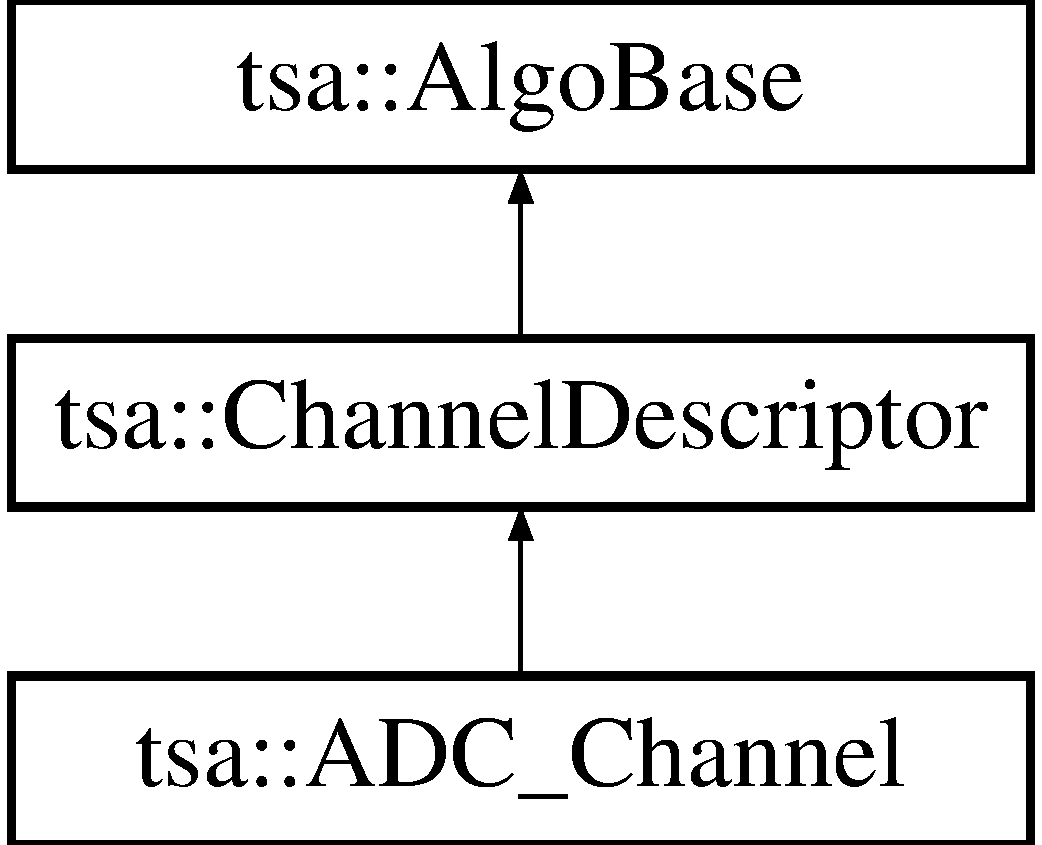
\includegraphics[height=3.000000cm]{classtsa_1_1_a_d_c___channel}
\end{center}
\end{figure}
\subsection*{Public Member Functions}
\begin{DoxyCompactItemize}
\item 
\hyperlink{classtsa_1_1_a_d_c___channel_a18595131ed55a3488ef56cfc0b39611d}{A\+D\+C\+\_\+\+Channel} (\hyperlink{classtsa_1_1_frame_i_stream}{Frame\+I\+Stream} $\ast$F\+IS, Fr\+Adc\+Data $\ast$adc, unsigned int id)
\item 
virtual \hyperlink{classtsa_1_1_a_d_c___channel_a0f9c5bbb98da25e712d4f6f8c078e658}{$\sim$\+A\+D\+C\+\_\+\+Channel} ()
\item 
virtual void \hyperlink{classtsa_1_1_a_d_c___channel_a23052bc47591e46246701ec0573c7902}{Add\+Data} ()
\item 
virtual double \hyperlink{classtsa_1_1_a_d_c___channel_ab5e23c219a7bf70866b05c9d3ad3da6f}{Get\+Length} ()
\end{DoxyCompactItemize}
\subsection*{Static Public Member Functions}
\begin{DoxyCompactItemize}
\item 
static \hyperlink{classtsa_1_1_a_d_c___channel}{A\+D\+C\+\_\+\+Channel} $\ast$ \hyperlink{classtsa_1_1_a_d_c___channel_a4585997f9f0029bb8d6fee7d36d33c92}{Create} (\hyperlink{classtsa_1_1_frame_i_stream}{Frame\+I\+Stream} $\ast$F\+IS, char $\ast$name, unsigned int id)
\end{DoxyCompactItemize}
\subsection*{Private Attributes}
\begin{DoxyCompactItemize}
\item 
char $\ast$ \hyperlink{classtsa_1_1_a_d_c___channel_a10f5984a8170a8cc68f5e78234166cd2}{m\+Name}
\end{DoxyCompactItemize}
\subsection*{Additional Inherited Members}


\subsection{Detailed Description}
A descriptor for an A\+DC channel 

Definition at line 230 of file Frame\+I\+Stream.\+hpp.



\subsection{Constructor \& Destructor Documentation}
\mbox{\Hypertarget{classtsa_1_1_a_d_c___channel_a18595131ed55a3488ef56cfc0b39611d}\label{classtsa_1_1_a_d_c___channel_a18595131ed55a3488ef56cfc0b39611d}} 
\index{tsa\+::\+A\+D\+C\+\_\+\+Channel@{tsa\+::\+A\+D\+C\+\_\+\+Channel}!A\+D\+C\+\_\+\+Channel@{A\+D\+C\+\_\+\+Channel}}
\index{A\+D\+C\+\_\+\+Channel@{A\+D\+C\+\_\+\+Channel}!tsa\+::\+A\+D\+C\+\_\+\+Channel@{tsa\+::\+A\+D\+C\+\_\+\+Channel}}
\subsubsection{\texorpdfstring{A\+D\+C\+\_\+\+Channel()}{ADC\_Channel()}}
{\footnotesize\ttfamily tsa\+::\+A\+D\+C\+\_\+\+Channel\+::\+A\+D\+C\+\_\+\+Channel (\begin{DoxyParamCaption}\item[{\hyperlink{classtsa_1_1_frame_i_stream}{Frame\+I\+Stream} $\ast$}]{F\+IS,  }\item[{Fr\+Adc\+Data $\ast$}]{adc,  }\item[{unsigned int}]{id }\end{DoxyParamCaption})}

Constructor


\begin{DoxyParams}{Parameters}
{\em F\+IS} & pointer to the \hyperlink{classtsa_1_1_frame_i_stream}{Frame\+I\+Stream} class \\
\hline
{\em adc} & pointer to the first Fr\+Adc\+Data structure \\
\hline
{\em id} & id of the channel \\
\hline
\end{DoxyParams}


Definition at line 229 of file Frame\+I\+Stream.\+cpp.

\mbox{\Hypertarget{classtsa_1_1_a_d_c___channel_a0f9c5bbb98da25e712d4f6f8c078e658}\label{classtsa_1_1_a_d_c___channel_a0f9c5bbb98da25e712d4f6f8c078e658}} 
\index{tsa\+::\+A\+D\+C\+\_\+\+Channel@{tsa\+::\+A\+D\+C\+\_\+\+Channel}!````~A\+D\+C\+\_\+\+Channel@{$\sim$\+A\+D\+C\+\_\+\+Channel}}
\index{````~A\+D\+C\+\_\+\+Channel@{$\sim$\+A\+D\+C\+\_\+\+Channel}!tsa\+::\+A\+D\+C\+\_\+\+Channel@{tsa\+::\+A\+D\+C\+\_\+\+Channel}}
\subsubsection{\texorpdfstring{$\sim$\+A\+D\+C\+\_\+\+Channel()}{~ADC\_Channel()}}
{\footnotesize\ttfamily tsa\+::\+A\+D\+C\+\_\+\+Channel\+::$\sim$\+A\+D\+C\+\_\+\+Channel (\begin{DoxyParamCaption}{ }\end{DoxyParamCaption})\hspace{0.3cm}{\ttfamily [virtual]}}

Destructor 

Definition at line 241 of file Frame\+I\+Stream.\+cpp.



\subsection{Member Function Documentation}
\mbox{\Hypertarget{classtsa_1_1_a_d_c___channel_a23052bc47591e46246701ec0573c7902}\label{classtsa_1_1_a_d_c___channel_a23052bc47591e46246701ec0573c7902}} 
\index{tsa\+::\+A\+D\+C\+\_\+\+Channel@{tsa\+::\+A\+D\+C\+\_\+\+Channel}!Add\+Data@{Add\+Data}}
\index{Add\+Data@{Add\+Data}!tsa\+::\+A\+D\+C\+\_\+\+Channel@{tsa\+::\+A\+D\+C\+\_\+\+Channel}}
\subsubsection{\texorpdfstring{Add\+Data()}{AddData()}}
{\footnotesize\ttfamily void tsa\+::\+A\+D\+C\+\_\+\+Channel\+::\+Add\+Data (\begin{DoxyParamCaption}{ }\end{DoxyParamCaption})\hspace{0.3cm}{\ttfamily [virtual]}}

This function must be called when there are not enough data to fill the output view. It reads a chunk of data from the current frame 

Reimplemented from \hyperlink{classtsa_1_1_channel_descriptor_aa1e001a5e712415cd4e9d66846914a56}{tsa\+::\+Channel\+Descriptor}.



Definition at line 245 of file Frame\+I\+Stream.\+cpp.

\mbox{\Hypertarget{classtsa_1_1_a_d_c___channel_a4585997f9f0029bb8d6fee7d36d33c92}\label{classtsa_1_1_a_d_c___channel_a4585997f9f0029bb8d6fee7d36d33c92}} 
\index{tsa\+::\+A\+D\+C\+\_\+\+Channel@{tsa\+::\+A\+D\+C\+\_\+\+Channel}!Create@{Create}}
\index{Create@{Create}!tsa\+::\+A\+D\+C\+\_\+\+Channel@{tsa\+::\+A\+D\+C\+\_\+\+Channel}}
\subsubsection{\texorpdfstring{Create()}{Create()}}
{\footnotesize\ttfamily \hyperlink{classtsa_1_1_a_d_c___channel}{A\+D\+C\+\_\+\+Channel} $\ast$ tsa\+::\+A\+D\+C\+\_\+\+Channel\+::\+Create (\begin{DoxyParamCaption}\item[{\hyperlink{classtsa_1_1_frame_i_stream}{Frame\+I\+Stream} $\ast$}]{F\+IS,  }\item[{char $\ast$}]{name,  }\item[{unsigned int}]{id }\end{DoxyParamCaption})\hspace{0.3cm}{\ttfamily [static]}}

Create, if possible, an instance of the class


\begin{DoxyParams}{Parameters}
{\em F\+IS} & pointer to the \hyperlink{classtsa_1_1_frame_i_stream}{Frame\+I\+Stream} class instance \\
\hline
{\em name} & name of the channel \\
\hline
{\em id} & index of the channel\\
\hline
\end{DoxyParams}
\begin{DoxyReturn}{Returns}
pointer to the created class instance or null 
\end{DoxyReturn}


Definition at line 218 of file Frame\+I\+Stream.\+cpp.

\mbox{\Hypertarget{classtsa_1_1_a_d_c___channel_ab5e23c219a7bf70866b05c9d3ad3da6f}\label{classtsa_1_1_a_d_c___channel_ab5e23c219a7bf70866b05c9d3ad3da6f}} 
\index{tsa\+::\+A\+D\+C\+\_\+\+Channel@{tsa\+::\+A\+D\+C\+\_\+\+Channel}!Get\+Length@{Get\+Length}}
\index{Get\+Length@{Get\+Length}!tsa\+::\+A\+D\+C\+\_\+\+Channel@{tsa\+::\+A\+D\+C\+\_\+\+Channel}}
\subsubsection{\texorpdfstring{Get\+Length()}{GetLength()}}
{\footnotesize\ttfamily double tsa\+::\+A\+D\+C\+\_\+\+Channel\+::\+Get\+Length (\begin{DoxyParamCaption}{ }\end{DoxyParamCaption})\hspace{0.3cm}{\ttfamily [virtual]}}

Get the maximul time length of data that can be currently filled without calling Add\+Data.

\begin{DoxyReturn}{Returns}
the time length of the data available in seconds 
\end{DoxyReturn}


Reimplemented from \hyperlink{classtsa_1_1_channel_descriptor_a456d14e6136c389fbd307fabab7d7b73}{tsa\+::\+Channel\+Descriptor}.



Definition at line 254 of file Frame\+I\+Stream.\+cpp.



\subsection{Member Data Documentation}
\mbox{\Hypertarget{classtsa_1_1_a_d_c___channel_a10f5984a8170a8cc68f5e78234166cd2}\label{classtsa_1_1_a_d_c___channel_a10f5984a8170a8cc68f5e78234166cd2}} 
\index{tsa\+::\+A\+D\+C\+\_\+\+Channel@{tsa\+::\+A\+D\+C\+\_\+\+Channel}!m\+Name@{m\+Name}}
\index{m\+Name@{m\+Name}!tsa\+::\+A\+D\+C\+\_\+\+Channel@{tsa\+::\+A\+D\+C\+\_\+\+Channel}}
\subsubsection{\texorpdfstring{m\+Name}{mName}}
{\footnotesize\ttfamily char$\ast$ tsa\+::\+A\+D\+C\+\_\+\+Channel\+::m\+Name\hspace{0.3cm}{\ttfamily [private]}}



Definition at line 276 of file Frame\+I\+Stream.\+hpp.



The documentation for this class was generated from the following files\+:\begin{DoxyCompactItemize}
\item 
/home/filip/\+Ph\+D/\+W\+D\+F\+Pipe\+\_\+test/p4\+T\+S\+A/include/\hyperlink{_frame_i_stream_8hpp}{Frame\+I\+Stream.\+hpp}\item 
/home/filip/\+Ph\+D/\+W\+D\+F\+Pipe\+\_\+test/p4\+T\+S\+A/src/\hyperlink{_frame_i_stream_8cpp}{Frame\+I\+Stream.\+cpp}\end{DoxyCompactItemize}

\hypertarget{classtsa_1_1_algo_base}{}\section{tsa\+:\+:Algo\+Base Class Reference}
\label{classtsa_1_1_algo_base}\index{tsa\+::\+Algo\+Base@{tsa\+::\+Algo\+Base}}


\hyperlink{classtsa_1_1_algo_base}{Algo\+Base} is the abstract base class for all algorithm.  




{\ttfamily \#include $<$Algo\+Base.\+hpp$>$}

Inheritance diagram for tsa\+:\+:Algo\+Base\+:\begin{figure}[H]
\begin{center}
\leavevmode
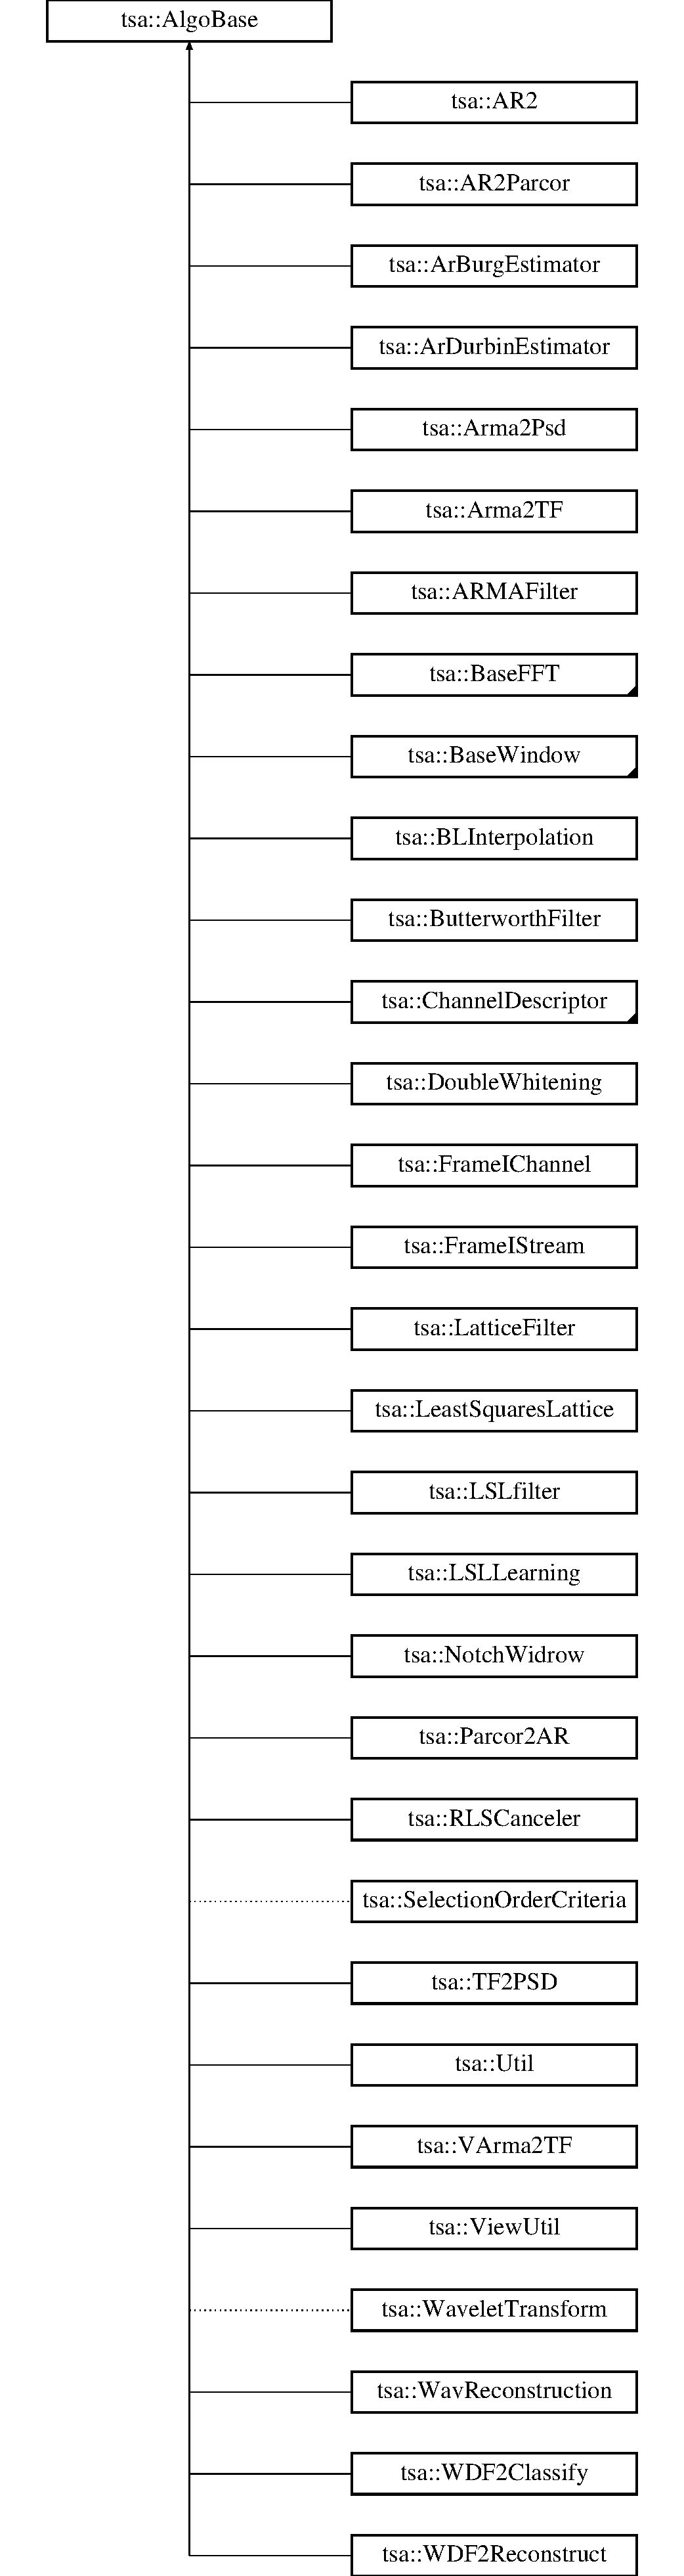
\includegraphics[height=12.000000cm]{classtsa_1_1_algo_base}
\end{center}
\end{figure}


\subsection{Detailed Description}
\hyperlink{classtsa_1_1_algo_base}{Algo\+Base} is the abstract base class for all algorithm. 

\hyperlink{classtsa_1_1_algo_base}{Algo\+Base} is the abstract base class for all the algorithm classes. It contain the definition of the common methods. An algorithm is a class with one or more execute() methods, with a variable number of parameters. 

Definition at line 64 of file Algo\+Base.\+hpp.



The documentation for this class was generated from the following file\+:\begin{DoxyCompactItemize}
\item 
/home/filip/\+Ph\+D/\+W\+D\+F\+Pipe\+\_\+test/p4\+T\+S\+A/include/\hyperlink{_algo_base_8hpp}{Algo\+Base.\+hpp}\end{DoxyCompactItemize}

\hypertarget{classtsa_1_1_a_r2}{}\section{tsa\+:\+:A\+R2 Class Reference}
\label{classtsa_1_1_a_r2}\index{tsa\+::\+A\+R2@{tsa\+::\+A\+R2}}


{\ttfamily \#include $<$A\+R2.\+hpp$>$}

Inheritance diagram for tsa\+:\+:A\+R2\+:\begin{figure}[H]
\begin{center}
\leavevmode
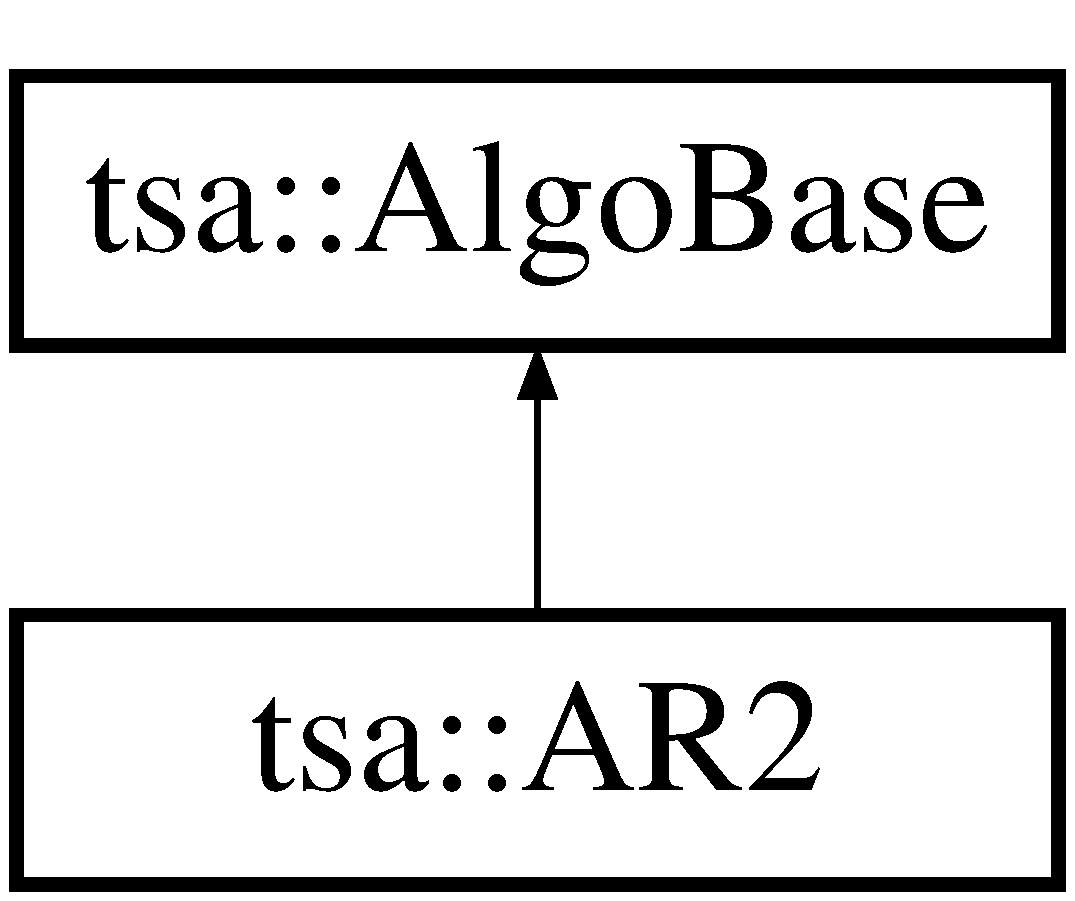
\includegraphics[height=2.000000cm]{classtsa_1_1_a_r2}
\end{center}
\end{figure}
\subsection*{Public Member Functions}
\begin{DoxyCompactItemize}
\item 
\hyperlink{classtsa_1_1_a_r2_af98beea50a63f72e22af69e2f1843bc3}{A\+R2} (const double f, const double gamma, const double h)
\item 
virtual \hyperlink{classtsa_1_1_a_r2_a69e035a519d396ff2ef47759d6394117}{$\sim$\+A\+R2} ()
\end{DoxyCompactItemize}
\begin{Indent}\textbf{ Operations}\par
\begin{DoxyCompactItemize}
\item 
void \hyperlink{classtsa_1_1_a_r2_ac99c0344d5376911a0976a78c0f8a96f}{operator()} (\hyperlink{namespacetsa_ac599574bcc094eda25613724b8f3ca9e}{Seq\+View\+Double} \&in, \hyperlink{namespacetsa_ac599574bcc094eda25613724b8f3ca9e}{Seq\+View\+Double} \&out)
\item 
void \hyperlink{classtsa_1_1_a_r2_a5a3bc7f3a15baca56a2660fff78259f9}{execute} (\hyperlink{namespacetsa_ad260cd21c1891c4ed391fe788569aba4}{Dmatrix} \&in, \hyperlink{namespacetsa_ad260cd21c1891c4ed391fe788569aba4}{Dmatrix} \&out, double scale)
\end{DoxyCompactItemize}
\end{Indent}
\subsection*{Private Attributes}
\begin{DoxyCompactItemize}
\item 
double \hyperlink{classtsa_1_1_a_r2_ad91c696d1eb47fb92e4440de0e871b34}{mA}
\item 
double \hyperlink{classtsa_1_1_a_r2_aa5edb94b32659768807f67f124b055f7}{mB}
\item 
double \hyperlink{classtsa_1_1_a_r2_a1e28277853e0e35cca6eb9a283cbc39e}{mC}
\item 
double \hyperlink{classtsa_1_1_a_r2_a855a67e26b267c41a48b5eb48d35ec06}{m\+Xm1}
\item 
double \hyperlink{classtsa_1_1_a_r2_add01d087af153e0addabb8c5b98318e4}{m\+Xm2}
\end{DoxyCompactItemize}


\subsection{Detailed Description}


Definition at line 70 of file A\+R2.\+hpp.



\subsection{Constructor \& Destructor Documentation}
\mbox{\Hypertarget{classtsa_1_1_a_r2_af98beea50a63f72e22af69e2f1843bc3}\label{classtsa_1_1_a_r2_af98beea50a63f72e22af69e2f1843bc3}} 
\index{tsa\+::\+A\+R2@{tsa\+::\+A\+R2}!A\+R2@{A\+R2}}
\index{A\+R2@{A\+R2}!tsa\+::\+A\+R2@{tsa\+::\+A\+R2}}
\subsubsection{\texorpdfstring{A\+R2()}{AR2()}}
{\footnotesize\ttfamily tsa\+::\+A\+R2\+::\+A\+R2 (\begin{DoxyParamCaption}\item[{const double}]{f,  }\item[{const double}]{gamma,  }\item[{const double}]{h }\end{DoxyParamCaption})}

Constructor 

Definition at line 5 of file A\+R2.\+cpp.

\mbox{\Hypertarget{classtsa_1_1_a_r2_a69e035a519d396ff2ef47759d6394117}\label{classtsa_1_1_a_r2_a69e035a519d396ff2ef47759d6394117}} 
\index{tsa\+::\+A\+R2@{tsa\+::\+A\+R2}!````~A\+R2@{$\sim$\+A\+R2}}
\index{````~A\+R2@{$\sim$\+A\+R2}!tsa\+::\+A\+R2@{tsa\+::\+A\+R2}}
\subsubsection{\texorpdfstring{$\sim$\+A\+R2()}{~AR2()}}
{\footnotesize\ttfamily tsa\+::\+A\+R2\+::$\sim$\+A\+R2 (\begin{DoxyParamCaption}{ }\end{DoxyParamCaption})\hspace{0.3cm}{\ttfamily [virtual]}}

Destructor 

Definition at line 15 of file A\+R2.\+cpp.



\subsection{Member Function Documentation}
\mbox{\Hypertarget{classtsa_1_1_a_r2_a5a3bc7f3a15baca56a2660fff78259f9}\label{classtsa_1_1_a_r2_a5a3bc7f3a15baca56a2660fff78259f9}} 
\index{tsa\+::\+A\+R2@{tsa\+::\+A\+R2}!execute@{execute}}
\index{execute@{execute}!tsa\+::\+A\+R2@{tsa\+::\+A\+R2}}
\subsubsection{\texorpdfstring{execute()}{execute()}}
{\footnotesize\ttfamily void tsa\+::\+A\+R2\+::execute (\begin{DoxyParamCaption}\item[{\hyperlink{namespacetsa_ad260cd21c1891c4ed391fe788569aba4}{Dmatrix} \&}]{in,  }\item[{\hyperlink{namespacetsa_ad260cd21c1891c4ed391fe788569aba4}{Dmatrix} \&}]{out,  }\item[{double}]{scale }\end{DoxyParamCaption})}


\begin{DoxyParams}{Parameters}
{\em in} & Input Data \\
\hline
{\em out} & Filtered Data \\
\hline
\end{DoxyParams}
\begin{DoxyReturn}{Returns}

\end{DoxyReturn}


Definition at line 36 of file A\+R2.\+cpp.

\mbox{\Hypertarget{classtsa_1_1_a_r2_ac99c0344d5376911a0976a78c0f8a96f}\label{classtsa_1_1_a_r2_ac99c0344d5376911a0976a78c0f8a96f}} 
\index{tsa\+::\+A\+R2@{tsa\+::\+A\+R2}!operator()@{operator()}}
\index{operator()@{operator()}!tsa\+::\+A\+R2@{tsa\+::\+A\+R2}}
\subsubsection{\texorpdfstring{operator()()}{operator()()}}
{\footnotesize\ttfamily void tsa\+::\+A\+R2\+::operator() (\begin{DoxyParamCaption}\item[{\hyperlink{namespacetsa_ac599574bcc094eda25613724b8f3ca9e}{Seq\+View\+Double} \&}]{in,  }\item[{\hyperlink{namespacetsa_ac599574bcc094eda25613724b8f3ca9e}{Seq\+View\+Double} \&}]{out }\end{DoxyParamCaption})}



Definition at line 19 of file A\+R2.\+cpp.



\subsection{Member Data Documentation}
\mbox{\Hypertarget{classtsa_1_1_a_r2_ad91c696d1eb47fb92e4440de0e871b34}\label{classtsa_1_1_a_r2_ad91c696d1eb47fb92e4440de0e871b34}} 
\index{tsa\+::\+A\+R2@{tsa\+::\+A\+R2}!mA@{mA}}
\index{mA@{mA}!tsa\+::\+A\+R2@{tsa\+::\+A\+R2}}
\subsubsection{\texorpdfstring{mA}{mA}}
{\footnotesize\ttfamily double tsa\+::\+A\+R2\+::mA\hspace{0.3cm}{\ttfamily [private]}}



Definition at line 124 of file A\+R2.\+hpp.

\mbox{\Hypertarget{classtsa_1_1_a_r2_aa5edb94b32659768807f67f124b055f7}\label{classtsa_1_1_a_r2_aa5edb94b32659768807f67f124b055f7}} 
\index{tsa\+::\+A\+R2@{tsa\+::\+A\+R2}!mB@{mB}}
\index{mB@{mB}!tsa\+::\+A\+R2@{tsa\+::\+A\+R2}}
\subsubsection{\texorpdfstring{mB}{mB}}
{\footnotesize\ttfamily double tsa\+::\+A\+R2\+::mB\hspace{0.3cm}{\ttfamily [private]}}



Definition at line 125 of file A\+R2.\+hpp.

\mbox{\Hypertarget{classtsa_1_1_a_r2_a1e28277853e0e35cca6eb9a283cbc39e}\label{classtsa_1_1_a_r2_a1e28277853e0e35cca6eb9a283cbc39e}} 
\index{tsa\+::\+A\+R2@{tsa\+::\+A\+R2}!mC@{mC}}
\index{mC@{mC}!tsa\+::\+A\+R2@{tsa\+::\+A\+R2}}
\subsubsection{\texorpdfstring{mC}{mC}}
{\footnotesize\ttfamily double tsa\+::\+A\+R2\+::mC\hspace{0.3cm}{\ttfamily [private]}}



Definition at line 126 of file A\+R2.\+hpp.

\mbox{\Hypertarget{classtsa_1_1_a_r2_a855a67e26b267c41a48b5eb48d35ec06}\label{classtsa_1_1_a_r2_a855a67e26b267c41a48b5eb48d35ec06}} 
\index{tsa\+::\+A\+R2@{tsa\+::\+A\+R2}!m\+Xm1@{m\+Xm1}}
\index{m\+Xm1@{m\+Xm1}!tsa\+::\+A\+R2@{tsa\+::\+A\+R2}}
\subsubsection{\texorpdfstring{m\+Xm1}{mXm1}}
{\footnotesize\ttfamily double tsa\+::\+A\+R2\+::m\+Xm1\hspace{0.3cm}{\ttfamily [private]}}



Definition at line 128 of file A\+R2.\+hpp.

\mbox{\Hypertarget{classtsa_1_1_a_r2_add01d087af153e0addabb8c5b98318e4}\label{classtsa_1_1_a_r2_add01d087af153e0addabb8c5b98318e4}} 
\index{tsa\+::\+A\+R2@{tsa\+::\+A\+R2}!m\+Xm2@{m\+Xm2}}
\index{m\+Xm2@{m\+Xm2}!tsa\+::\+A\+R2@{tsa\+::\+A\+R2}}
\subsubsection{\texorpdfstring{m\+Xm2}{mXm2}}
{\footnotesize\ttfamily double tsa\+::\+A\+R2\+::m\+Xm2\hspace{0.3cm}{\ttfamily [private]}}



Definition at line 129 of file A\+R2.\+hpp.



The documentation for this class was generated from the following files\+:\begin{DoxyCompactItemize}
\item 
/home/filip/\+Ph\+D/\+W\+D\+F\+Pipe\+\_\+test/p4\+T\+S\+A/include/\hyperlink{_a_r2_8hpp}{A\+R2.\+hpp}\item 
/home/filip/\+Ph\+D/\+W\+D\+F\+Pipe\+\_\+test/p4\+T\+S\+A/src/\hyperlink{_a_r2_8cpp}{A\+R2.\+cpp}\end{DoxyCompactItemize}

\hypertarget{classtsa_1_1_a_r2_parcor}{}\section{tsa\+:\+:A\+R2\+Parcor Class Reference}
\label{classtsa_1_1_a_r2_parcor}\index{tsa\+::\+A\+R2\+Parcor@{tsa\+::\+A\+R2\+Parcor}}


Estimate the AR parameters by the Parcor.  




{\ttfamily \#include $<$A\+R2\+Parcor.\+hpp$>$}

Inheritance diagram for tsa\+:\+:A\+R2\+Parcor\+:\begin{figure}[H]
\begin{center}
\leavevmode
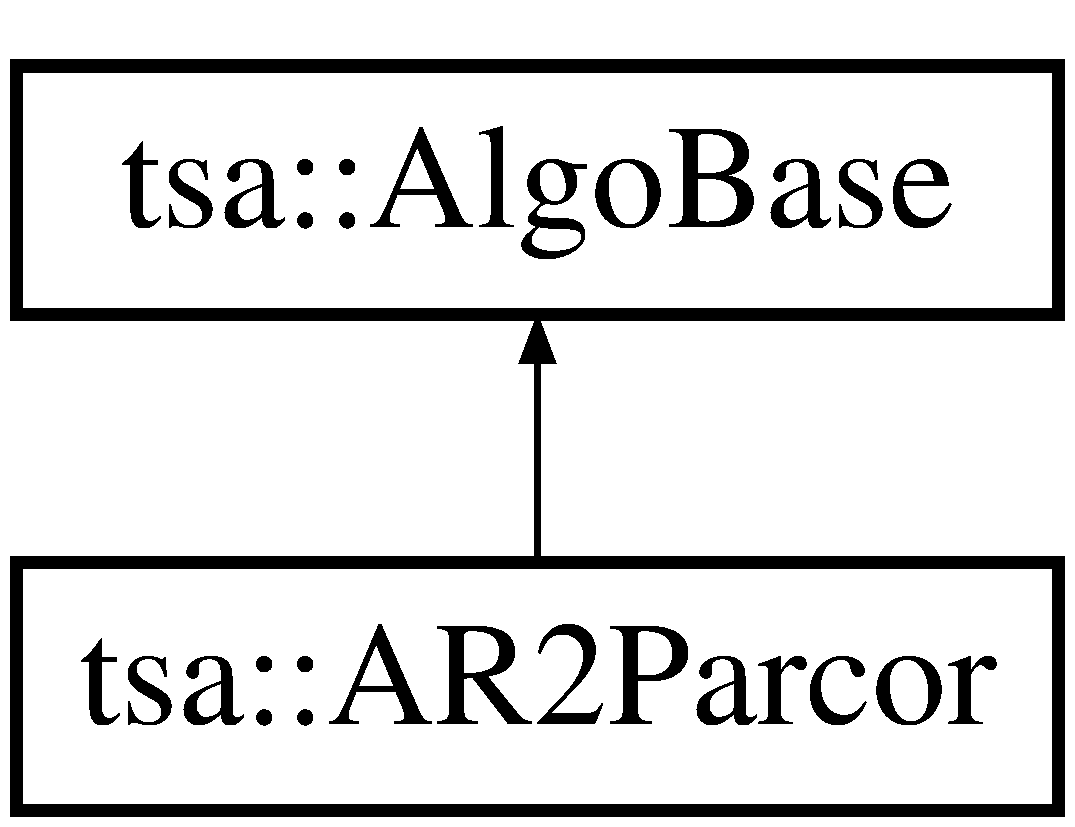
\includegraphics[height=2.000000cm]{classtsa_1_1_a_r2_parcor}
\end{center}
\end{figure}
\subsection*{Public Member Functions}
\begin{DoxyCompactItemize}
\item 
\hyperlink{classtsa_1_1_a_r2_parcor_af28c0ed978d27202d9f7f5df6464efef}{A\+R2\+Parcor} ()
\item 
virtual \hyperlink{classtsa_1_1_a_r2_parcor_a8aaf9b98dd73626724c6c83bf7e3a5ed}{$\sim$\+A\+R2\+Parcor} ()
\end{DoxyCompactItemize}
\begin{Indent}\textbf{ Operations}\par
\begin{DoxyCompactItemize}
\item 
void \hyperlink{classtsa_1_1_a_r2_parcor_a238bba748285d03e10622d2f2f0cc108}{execute} (\hyperlink{namespacetsa_a8900fb03d849baf447a1a0efe2561fb2}{Dvector} \&AR, \hyperlink{namespacetsa_a8900fb03d849baf447a1a0efe2561fb2}{Dvector} \&Parcor)
\end{DoxyCompactItemize}
\end{Indent}


\subsection{Detailed Description}
Estimate the AR parameters by the Parcor. 

Definition at line 71 of file A\+R2\+Parcor.\+hpp.



\subsection{Constructor \& Destructor Documentation}
\mbox{\Hypertarget{classtsa_1_1_a_r2_parcor_af28c0ed978d27202d9f7f5df6464efef}\label{classtsa_1_1_a_r2_parcor_af28c0ed978d27202d9f7f5df6464efef}} 
\index{tsa\+::\+A\+R2\+Parcor@{tsa\+::\+A\+R2\+Parcor}!A\+R2\+Parcor@{A\+R2\+Parcor}}
\index{A\+R2\+Parcor@{A\+R2\+Parcor}!tsa\+::\+A\+R2\+Parcor@{tsa\+::\+A\+R2\+Parcor}}
\subsubsection{\texorpdfstring{A\+R2\+Parcor()}{AR2Parcor()}}
{\footnotesize\ttfamily tsa\+::\+A\+R2\+Parcor\+::\+A\+R2\+Parcor (\begin{DoxyParamCaption}{ }\end{DoxyParamCaption})}

Constructor 

Definition at line 19 of file A\+R2\+Parcor.\+cpp.

\mbox{\Hypertarget{classtsa_1_1_a_r2_parcor_a8aaf9b98dd73626724c6c83bf7e3a5ed}\label{classtsa_1_1_a_r2_parcor_a8aaf9b98dd73626724c6c83bf7e3a5ed}} 
\index{tsa\+::\+A\+R2\+Parcor@{tsa\+::\+A\+R2\+Parcor}!````~A\+R2\+Parcor@{$\sim$\+A\+R2\+Parcor}}
\index{````~A\+R2\+Parcor@{$\sim$\+A\+R2\+Parcor}!tsa\+::\+A\+R2\+Parcor@{tsa\+::\+A\+R2\+Parcor}}
\subsubsection{\texorpdfstring{$\sim$\+A\+R2\+Parcor()}{~AR2Parcor()}}
{\footnotesize\ttfamily tsa\+::\+A\+R2\+Parcor\+::$\sim$\+A\+R2\+Parcor (\begin{DoxyParamCaption}{ }\end{DoxyParamCaption})\hspace{0.3cm}{\ttfamily [virtual]}}

Destructor 

Definition at line 22 of file A\+R2\+Parcor.\+cpp.



\subsection{Member Function Documentation}
\mbox{\Hypertarget{classtsa_1_1_a_r2_parcor_a238bba748285d03e10622d2f2f0cc108}\label{classtsa_1_1_a_r2_parcor_a238bba748285d03e10622d2f2f0cc108}} 
\index{tsa\+::\+A\+R2\+Parcor@{tsa\+::\+A\+R2\+Parcor}!execute@{execute}}
\index{execute@{execute}!tsa\+::\+A\+R2\+Parcor@{tsa\+::\+A\+R2\+Parcor}}
\subsubsection{\texorpdfstring{execute()}{execute()}}
{\footnotesize\ttfamily void tsa\+::\+A\+R2\+Parcor\+::execute (\begin{DoxyParamCaption}\item[{\hyperlink{namespacetsa_a8900fb03d849baf447a1a0efe2561fb2}{Dvector} \&}]{AR,  }\item[{\hyperlink{namespacetsa_a8900fb03d849baf447a1a0efe2561fb2}{Dvector} \&}]{Parcor }\end{DoxyParamCaption})}

The execute method transform the parcor in AR


\begin{DoxyParams}{Parameters}
{\em Parcor} & reflection coefficients vector \\
\hline
{\em AR} & autoregressive parameters \\
\hline
\end{DoxyParams}


Definition at line 25 of file A\+R2\+Parcor.\+cpp.



The documentation for this class was generated from the following files\+:\begin{DoxyCompactItemize}
\item 
/home/filip/\+Ph\+D/\+W\+D\+F\+Pipe\+\_\+test/p4\+T\+S\+A/include/\hyperlink{_a_r2_parcor_8hpp}{A\+R2\+Parcor.\+hpp}\item 
/home/filip/\+Ph\+D/\+W\+D\+F\+Pipe\+\_\+test/p4\+T\+S\+A/src/\hyperlink{_a_r2_parcor_8cpp}{A\+R2\+Parcor.\+cpp}\end{DoxyCompactItemize}

\hypertarget{classtsa_1_1_ar_burg_estimator}{}\section{tsa\+:\+:Ar\+Burg\+Estimator Class Reference}
\label{classtsa_1_1_ar_burg_estimator}\index{tsa\+::\+Ar\+Burg\+Estimator@{tsa\+::\+Ar\+Burg\+Estimator}}


Estimate the Parcor and AR parameters on a sequence of data.  




{\ttfamily \#include $<$Ar\+Burg\+Estimator.\+hpp$>$}

Inheritance diagram for tsa\+:\+:Ar\+Burg\+Estimator\+:\begin{figure}[H]
\begin{center}
\leavevmode
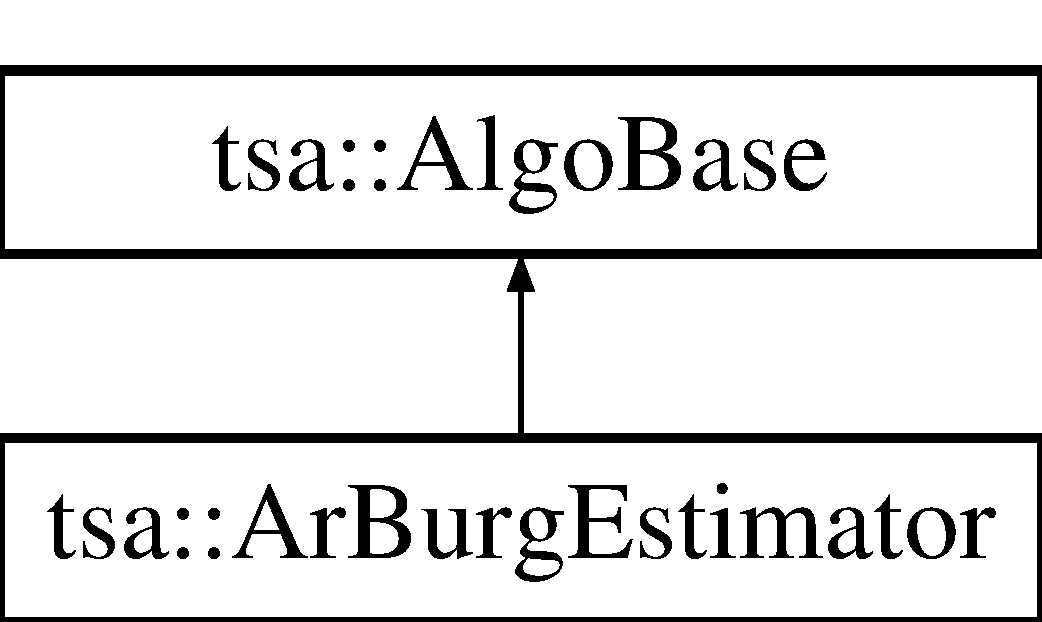
\includegraphics[height=2.000000cm]{classtsa_1_1_ar_burg_estimator}
\end{center}
\end{figure}
\subsection*{Public Member Functions}
\begin{DoxyCompactItemize}
\item 
\hyperlink{classtsa_1_1_ar_burg_estimator_a6204df3016ce1f4aabf95fe4e05b27c4}{Ar\+Burg\+Estimator} (unsigned int Ar\+Order)
\item 
virtual \hyperlink{classtsa_1_1_ar_burg_estimator_a4b72f798ee5330d446366c4296aec27b}{$\sim$\+Ar\+Burg\+Estimator} ()
\item 
void \hyperlink{classtsa_1_1_ar_burg_estimator_a909ccc5f3ec7155ca60fb23122a8edfd}{Load} (const char $\ast$filename, const char $\ast$fmt=\char`\"{}txt\char`\"{})
\item 
void \hyperlink{classtsa_1_1_ar_burg_estimator_a5f666a51727cfd49d748973b8f050763}{Save} (const char $\ast$filename, const char $\ast$fmt=\char`\"{}txt\char`\"{})
\item 
void \hyperlink{classtsa_1_1_ar_burg_estimator_a2760a49fb1837ff81061ebf7431de0ef}{xml\+\_\+serialize} (\hyperlink{classeternity_1_1xml__archive}{eternity\+::xml\+\_\+archive} \&xml, const char $\ast$prefix)
\end{DoxyCompactItemize}
\begin{Indent}\textbf{ Operations}\par
\begin{DoxyCompactItemize}
\item 
void \hyperlink{classtsa_1_1_ar_burg_estimator_a904c4776668339798aa429622989dae6}{operator()} (\hyperlink{namespacetsa_ac599574bcc094eda25613724b8f3ca9e}{Seq\+View\+Double} \&Input\+Data, \hyperlink{namespacetsa_ac599574bcc094eda25613724b8f3ca9e}{Seq\+View\+Double} \&Whitened\+Data)
\item 
void \hyperlink{classtsa_1_1_ar_burg_estimator_a4c318ac037fabbad13f506e97576034a}{Color} (\hyperlink{namespacetsa_ac599574bcc094eda25613724b8f3ca9e}{Seq\+View\+Double} \&Whitened\+Data, \hyperlink{namespacetsa_ac599574bcc094eda25613724b8f3ca9e}{Seq\+View\+Double} \&Colored\+Data)
\item 
void \hyperlink{classtsa_1_1_ar_burg_estimator_a84c6368cebbbe6965e28769e406d4310}{operator()} (\hyperlink{namespacetsa_ac599574bcc094eda25613724b8f3ca9e}{Seq\+View\+Double} \&Input\+Data)
\item 
void \hyperlink{classtsa_1_1_ar_burg_estimator_aab366c108b53cb7d4ac5b76d5f6ac465}{execute} (matrix\+\_\+row$<$ \hyperlink{namespacetsa_ad260cd21c1891c4ed391fe788569aba4}{Dmatrix} $>$ Input\+Data)
\begin{DoxyCompactList}\small\item\em Estimate the Parcor and AR parameters on a sequence of data. \end{DoxyCompactList}\item 
void \hyperlink{classtsa_1_1_ar_burg_estimator_a3b6d9a2e792b5cd1abb9c8daadc15cac}{color} (matrix\+\_\+row$<$ \hyperlink{namespacetsa_ad260cd21c1891c4ed391fe788569aba4}{Dmatrix} $>$ Whitened\+Data, matrix\+\_\+row$<$ \hyperlink{namespacetsa_ad260cd21c1891c4ed391fe788569aba4}{Dmatrix} $>$ Colored\+Data)
\end{DoxyCompactItemize}
\end{Indent}
\begin{Indent}\textbf{ Getters}\par
\begin{DoxyCompactItemize}
\item 
void \hyperlink{classtsa_1_1_ar_burg_estimator_a06b9a3daeecfcc31d6c5e617848ee200}{Get\+Lattice\+View} (\hyperlink{classtsa_1_1_lattice_view}{Lattice\+View} \&LV)
\item 
unsigned int \hyperlink{classtsa_1_1_ar_burg_estimator_a61a8a96608a0d354a1dd942cdf71c669}{Get\+Ar\+Order} ()
\item 
double \hyperlink{classtsa_1_1_ar_burg_estimator_abfbc945d2915208835f1bce7062a14c4}{Get\+Parcor} (unsigned int j)
\item 
double \hyperlink{classtsa_1_1_ar_burg_estimator_ae896885d9fcc18375eb2d3c00f3ceec7}{Get\+AR} (unsigned int j)
\item 
double \hyperlink{classtsa_1_1_ar_burg_estimator_a63e4fbfbd1245e1a899cc783c77f5bfd}{Get\+Error\+Forward} (unsigned int j)
\item 
double \hyperlink{classtsa_1_1_ar_burg_estimator_ae12190c986e02299da186dc29e97cded}{Get\+Error\+Backward} (unsigned int j)
\end{DoxyCompactItemize}
\end{Indent}
\begin{Indent}\textbf{ Setters}\par
\begin{DoxyCompactItemize}
\item 
void \hyperlink{classtsa_1_1_ar_burg_estimator_acbf9046f1ff3d7e2852ec4daa30ac8af}{Set\+Ar\+Order} (unsigned int P)
\begin{DoxyCompactList}\small\item\em setters \end{DoxyCompactList}\item 
void \hyperlink{classtsa_1_1_ar_burg_estimator_ae3873be61a19beab0b5b6e915c594889}{Set\+AR} (unsigned int j, double value)
\end{DoxyCompactItemize}
\end{Indent}
\subsection*{Private Attributes}
\begin{DoxyCompactItemize}
\item 
unsigned int \hyperlink{classtsa_1_1_ar_burg_estimator_a918baccfeb2101848018b6abcf1e9b19}{m\+Ar\+Order}
\item 
\hyperlink{namespacetsa_a8900fb03d849baf447a1a0efe2561fb2}{Dvector} \hyperlink{classtsa_1_1_ar_burg_estimator_a51cbda2be55098f65e4d710cfe1153b7}{m\+Parcor}
\item 
\hyperlink{namespacetsa_a8900fb03d849baf447a1a0efe2561fb2}{Dvector} \hyperlink{classtsa_1_1_ar_burg_estimator_a6d0a5657630ecd64c33761a8f0c835e1}{m\+AR}
\item 
\hyperlink{namespacetsa_a8900fb03d849baf447a1a0efe2561fb2}{Dvector} \hyperlink{classtsa_1_1_ar_burg_estimator_a3ff0b47d541f89567d177a42103a95a2}{m\+Error\+Forward}
\item 
\hyperlink{namespacetsa_a8900fb03d849baf447a1a0efe2561fb2}{Dvector} \hyperlink{classtsa_1_1_ar_burg_estimator_abe77e4f47e6eb9e1f39e22f99331c981}{m\+Error\+Backward}
\item 
\hyperlink{namespacetsa_a8900fb03d849baf447a1a0efe2561fb2}{Dvector} \hyperlink{classtsa_1_1_ar_burg_estimator_a3d033517e7242d079e14038dcd50556c}{m\+Whitened\+Data}
\item 
\hyperlink{namespacetsa_a8900fb03d849baf447a1a0efe2561fb2}{Dvector} \hyperlink{classtsa_1_1_ar_burg_estimator_a7b50a6b230b2236500f54f9561d9ef7d}{m\+Colored\+Data}
\end{DoxyCompactItemize}


\subsection{Detailed Description}
Estimate the Parcor and AR parameters on a sequence of data. 

Definition at line 77 of file Ar\+Burg\+Estimator.\+hpp.



\subsection{Constructor \& Destructor Documentation}
\mbox{\Hypertarget{classtsa_1_1_ar_burg_estimator_a6204df3016ce1f4aabf95fe4e05b27c4}\label{classtsa_1_1_ar_burg_estimator_a6204df3016ce1f4aabf95fe4e05b27c4}} 
\index{tsa\+::\+Ar\+Burg\+Estimator@{tsa\+::\+Ar\+Burg\+Estimator}!Ar\+Burg\+Estimator@{Ar\+Burg\+Estimator}}
\index{Ar\+Burg\+Estimator@{Ar\+Burg\+Estimator}!tsa\+::\+Ar\+Burg\+Estimator@{tsa\+::\+Ar\+Burg\+Estimator}}
\subsubsection{\texorpdfstring{Ar\+Burg\+Estimator()}{ArBurgEstimator()}}
{\footnotesize\ttfamily tsa\+::\+Ar\+Burg\+Estimator\+::\+Ar\+Burg\+Estimator (\begin{DoxyParamCaption}\item[{unsigned int}]{Ar\+Order }\end{DoxyParamCaption})}

Constructor 
\begin{DoxyParams}{Parameters}
{\em Ar\+Order} & order of the AR model \\
\hline
\end{DoxyParams}


Definition at line 20 of file Ar\+Burg\+Estimator.\+cpp.

\mbox{\Hypertarget{classtsa_1_1_ar_burg_estimator_a4b72f798ee5330d446366c4296aec27b}\label{classtsa_1_1_ar_burg_estimator_a4b72f798ee5330d446366c4296aec27b}} 
\index{tsa\+::\+Ar\+Burg\+Estimator@{tsa\+::\+Ar\+Burg\+Estimator}!````~Ar\+Burg\+Estimator@{$\sim$\+Ar\+Burg\+Estimator}}
\index{````~Ar\+Burg\+Estimator@{$\sim$\+Ar\+Burg\+Estimator}!tsa\+::\+Ar\+Burg\+Estimator@{tsa\+::\+Ar\+Burg\+Estimator}}
\subsubsection{\texorpdfstring{$\sim$\+Ar\+Burg\+Estimator()}{~ArBurgEstimator()}}
{\footnotesize\ttfamily tsa\+::\+Ar\+Burg\+Estimator\+::$\sim$\+Ar\+Burg\+Estimator (\begin{DoxyParamCaption}{ }\end{DoxyParamCaption})\hspace{0.3cm}{\ttfamily [virtual]}}

Destructor 

Definition at line 29 of file Ar\+Burg\+Estimator.\+cpp.



\subsection{Member Function Documentation}
\mbox{\Hypertarget{classtsa_1_1_ar_burg_estimator_a4c318ac037fabbad13f506e97576034a}\label{classtsa_1_1_ar_burg_estimator_a4c318ac037fabbad13f506e97576034a}} 
\index{tsa\+::\+Ar\+Burg\+Estimator@{tsa\+::\+Ar\+Burg\+Estimator}!Color@{Color}}
\index{Color@{Color}!tsa\+::\+Ar\+Burg\+Estimator@{tsa\+::\+Ar\+Burg\+Estimator}}
\subsubsection{\texorpdfstring{Color()}{Color()}}
{\footnotesize\ttfamily void tsa\+::\+Ar\+Burg\+Estimator\+::\+Color (\begin{DoxyParamCaption}\item[{\hyperlink{namespacetsa_ac599574bcc094eda25613724b8f3ca9e}{Seq\+View\+Double} \&}]{Whitened\+Data,  }\item[{\hyperlink{namespacetsa_ac599574bcc094eda25613724b8f3ca9e}{Seq\+View\+Double} \&}]{Colored\+Data }\end{DoxyParamCaption})}

Implements the estimation of the AR paramenters using the Burg method.


\begin{DoxyParams}{Parameters}
{\em Input\+Data} & Input data time series \\
\hline
{\em Whitened\+Data} & Whitened time series \\
\hline
\end{DoxyParams}


Definition at line 54 of file Ar\+Burg\+Estimator.\+cpp.

\mbox{\Hypertarget{classtsa_1_1_ar_burg_estimator_a3b6d9a2e792b5cd1abb9c8daadc15cac}\label{classtsa_1_1_ar_burg_estimator_a3b6d9a2e792b5cd1abb9c8daadc15cac}} 
\index{tsa\+::\+Ar\+Burg\+Estimator@{tsa\+::\+Ar\+Burg\+Estimator}!color@{color}}
\index{color@{color}!tsa\+::\+Ar\+Burg\+Estimator@{tsa\+::\+Ar\+Burg\+Estimator}}
\subsubsection{\texorpdfstring{color()}{color()}}
{\footnotesize\ttfamily void tsa\+::\+Ar\+Burg\+Estimator\+::color (\begin{DoxyParamCaption}\item[{matrix\+\_\+row$<$ \hyperlink{namespacetsa_ad260cd21c1891c4ed391fe788569aba4}{Dmatrix} $>$}]{Whitened\+Data,  }\item[{matrix\+\_\+row$<$ \hyperlink{namespacetsa_ad260cd21c1891c4ed391fe788569aba4}{Dmatrix} $>$}]{Colored\+Data }\end{DoxyParamCaption})}



Definition at line 142 of file Ar\+Burg\+Estimator.\+cpp.

\mbox{\Hypertarget{classtsa_1_1_ar_burg_estimator_aab366c108b53cb7d4ac5b76d5f6ac465}\label{classtsa_1_1_ar_burg_estimator_aab366c108b53cb7d4ac5b76d5f6ac465}} 
\index{tsa\+::\+Ar\+Burg\+Estimator@{tsa\+::\+Ar\+Burg\+Estimator}!execute@{execute}}
\index{execute@{execute}!tsa\+::\+Ar\+Burg\+Estimator@{tsa\+::\+Ar\+Burg\+Estimator}}
\subsubsection{\texorpdfstring{execute()}{execute()}}
{\footnotesize\ttfamily void tsa\+::\+Ar\+Burg\+Estimator\+::execute (\begin{DoxyParamCaption}\item[{matrix\+\_\+row$<$ \hyperlink{namespacetsa_ad260cd21c1891c4ed391fe788569aba4}{Dmatrix} $>$}]{Input\+Data }\end{DoxyParamCaption})}



Estimate the Parcor and AR parameters on a sequence of data. 

\begin{DoxyPrecond}{Precondition}
The lenght of the input sequence must be greater then the AR order 
\end{DoxyPrecond}
\begin{DoxyRefDesc}{Todo}
\item[\hyperlink{todo__todo000002}{Todo}]Add execption\end{DoxyRefDesc}



\begin{DoxyParams}{Parameters}
{\em Input\+Data} & is the input sequences of data \\
\hline
\end{DoxyParams}
contain the norm of the input data 

Definition at line 79 of file Ar\+Burg\+Estimator.\+cpp.

\mbox{\Hypertarget{classtsa_1_1_ar_burg_estimator_ae896885d9fcc18375eb2d3c00f3ceec7}\label{classtsa_1_1_ar_burg_estimator_ae896885d9fcc18375eb2d3c00f3ceec7}} 
\index{tsa\+::\+Ar\+Burg\+Estimator@{tsa\+::\+Ar\+Burg\+Estimator}!Get\+AR@{Get\+AR}}
\index{Get\+AR@{Get\+AR}!tsa\+::\+Ar\+Burg\+Estimator@{tsa\+::\+Ar\+Burg\+Estimator}}
\subsubsection{\texorpdfstring{Get\+A\+R()}{GetAR()}}
{\footnotesize\ttfamily double tsa\+::\+Ar\+Burg\+Estimator\+::\+Get\+AR (\begin{DoxyParamCaption}\item[{unsigned int}]{j }\end{DoxyParamCaption})}

\begin{DoxyReturn}{Returns}
Get The AR values 
\end{DoxyReturn}


Definition at line 193 of file Ar\+Burg\+Estimator.\+cpp.

\mbox{\Hypertarget{classtsa_1_1_ar_burg_estimator_a61a8a96608a0d354a1dd942cdf71c669}\label{classtsa_1_1_ar_burg_estimator_a61a8a96608a0d354a1dd942cdf71c669}} 
\index{tsa\+::\+Ar\+Burg\+Estimator@{tsa\+::\+Ar\+Burg\+Estimator}!Get\+Ar\+Order@{Get\+Ar\+Order}}
\index{Get\+Ar\+Order@{Get\+Ar\+Order}!tsa\+::\+Ar\+Burg\+Estimator@{tsa\+::\+Ar\+Burg\+Estimator}}
\subsubsection{\texorpdfstring{Get\+Ar\+Order()}{GetArOrder()}}
{\footnotesize\ttfamily unsigned int tsa\+::\+Ar\+Burg\+Estimator\+::\+Get\+Ar\+Order (\begin{DoxyParamCaption}{ }\end{DoxyParamCaption})}

\begin{DoxyReturn}{Returns}
the Ar Order 
\end{DoxyReturn}


Definition at line 185 of file Ar\+Burg\+Estimator.\+cpp.

\mbox{\Hypertarget{classtsa_1_1_ar_burg_estimator_ae12190c986e02299da186dc29e97cded}\label{classtsa_1_1_ar_burg_estimator_ae12190c986e02299da186dc29e97cded}} 
\index{tsa\+::\+Ar\+Burg\+Estimator@{tsa\+::\+Ar\+Burg\+Estimator}!Get\+Error\+Backward@{Get\+Error\+Backward}}
\index{Get\+Error\+Backward@{Get\+Error\+Backward}!tsa\+::\+Ar\+Burg\+Estimator@{tsa\+::\+Ar\+Burg\+Estimator}}
\subsubsection{\texorpdfstring{Get\+Error\+Backward()}{GetErrorBackward()}}
{\footnotesize\ttfamily double tsa\+::\+Ar\+Burg\+Estimator\+::\+Get\+Error\+Backward (\begin{DoxyParamCaption}\item[{unsigned int}]{j }\end{DoxyParamCaption})}

\begin{DoxyReturn}{Returns}
Get the Error\+Backward values 
\end{DoxyReturn}


Definition at line 201 of file Ar\+Burg\+Estimator.\+cpp.

\mbox{\Hypertarget{classtsa_1_1_ar_burg_estimator_a63e4fbfbd1245e1a899cc783c77f5bfd}\label{classtsa_1_1_ar_burg_estimator_a63e4fbfbd1245e1a899cc783c77f5bfd}} 
\index{tsa\+::\+Ar\+Burg\+Estimator@{tsa\+::\+Ar\+Burg\+Estimator}!Get\+Error\+Forward@{Get\+Error\+Forward}}
\index{Get\+Error\+Forward@{Get\+Error\+Forward}!tsa\+::\+Ar\+Burg\+Estimator@{tsa\+::\+Ar\+Burg\+Estimator}}
\subsubsection{\texorpdfstring{Get\+Error\+Forward()}{GetErrorForward()}}
{\footnotesize\ttfamily double tsa\+::\+Ar\+Burg\+Estimator\+::\+Get\+Error\+Forward (\begin{DoxyParamCaption}\item[{unsigned int}]{j }\end{DoxyParamCaption})}

\begin{DoxyReturn}{Returns}
Get the Error\+Forward values 
\end{DoxyReturn}


Definition at line 197 of file Ar\+Burg\+Estimator.\+cpp.

\mbox{\Hypertarget{classtsa_1_1_ar_burg_estimator_a06b9a3daeecfcc31d6c5e617848ee200}\label{classtsa_1_1_ar_burg_estimator_a06b9a3daeecfcc31d6c5e617848ee200}} 
\index{tsa\+::\+Ar\+Burg\+Estimator@{tsa\+::\+Ar\+Burg\+Estimator}!Get\+Lattice\+View@{Get\+Lattice\+View}}
\index{Get\+Lattice\+View@{Get\+Lattice\+View}!tsa\+::\+Ar\+Burg\+Estimator@{tsa\+::\+Ar\+Burg\+Estimator}}
\subsubsection{\texorpdfstring{Get\+Lattice\+View()}{GetLatticeView()}}
{\footnotesize\ttfamily void tsa\+::\+Ar\+Burg\+Estimator\+::\+Get\+Lattice\+View (\begin{DoxyParamCaption}\item[{\hyperlink{classtsa_1_1_lattice_view}{Lattice\+View} \&}]{LV }\end{DoxyParamCaption})}


\begin{DoxyParams}{Parameters}
{\em LV} & the target lattice view \\
\hline
\end{DoxyParams}


Definition at line 168 of file Ar\+Burg\+Estimator.\+cpp.

\mbox{\Hypertarget{classtsa_1_1_ar_burg_estimator_abfbc945d2915208835f1bce7062a14c4}\label{classtsa_1_1_ar_burg_estimator_abfbc945d2915208835f1bce7062a14c4}} 
\index{tsa\+::\+Ar\+Burg\+Estimator@{tsa\+::\+Ar\+Burg\+Estimator}!Get\+Parcor@{Get\+Parcor}}
\index{Get\+Parcor@{Get\+Parcor}!tsa\+::\+Ar\+Burg\+Estimator@{tsa\+::\+Ar\+Burg\+Estimator}}
\subsubsection{\texorpdfstring{Get\+Parcor()}{GetParcor()}}
{\footnotesize\ttfamily double tsa\+::\+Ar\+Burg\+Estimator\+::\+Get\+Parcor (\begin{DoxyParamCaption}\item[{unsigned int}]{j }\end{DoxyParamCaption})}

\begin{DoxyReturn}{Returns}
Get The Parcor values 
\end{DoxyReturn}


Definition at line 189 of file Ar\+Burg\+Estimator.\+cpp.

\mbox{\Hypertarget{classtsa_1_1_ar_burg_estimator_a909ccc5f3ec7155ca60fb23122a8edfd}\label{classtsa_1_1_ar_burg_estimator_a909ccc5f3ec7155ca60fb23122a8edfd}} 
\index{tsa\+::\+Ar\+Burg\+Estimator@{tsa\+::\+Ar\+Burg\+Estimator}!Load@{Load}}
\index{Load@{Load}!tsa\+::\+Ar\+Burg\+Estimator@{tsa\+::\+Ar\+Burg\+Estimator}}
\subsubsection{\texorpdfstring{Load()}{Load()}}
{\footnotesize\ttfamily void tsa\+::\+Ar\+Burg\+Estimator\+::\+Load (\begin{DoxyParamCaption}\item[{const char $\ast$}]{filename,  }\item[{const char $\ast$}]{fmt = {\ttfamily \char`\"{}txt\char`\"{}} }\end{DoxyParamCaption})\hspace{0.3cm}{\ttfamily [inline]}}



Definition at line 91 of file Ar\+Burg\+Estimator.\+hpp.

\mbox{\Hypertarget{classtsa_1_1_ar_burg_estimator_a904c4776668339798aa429622989dae6}\label{classtsa_1_1_ar_burg_estimator_a904c4776668339798aa429622989dae6}} 
\index{tsa\+::\+Ar\+Burg\+Estimator@{tsa\+::\+Ar\+Burg\+Estimator}!operator()@{operator()}}
\index{operator()@{operator()}!tsa\+::\+Ar\+Burg\+Estimator@{tsa\+::\+Ar\+Burg\+Estimator}}
\subsubsection{\texorpdfstring{operator()()}{operator()()}\hspace{0.1cm}{\footnotesize\ttfamily [1/2]}}
{\footnotesize\ttfamily void tsa\+::\+Ar\+Burg\+Estimator\+::operator() (\begin{DoxyParamCaption}\item[{\hyperlink{namespacetsa_ac599574bcc094eda25613724b8f3ca9e}{Seq\+View\+Double} \&}]{Input\+Data,  }\item[{\hyperlink{namespacetsa_ac599574bcc094eda25613724b8f3ca9e}{Seq\+View\+Double} \&}]{Whitened\+Data }\end{DoxyParamCaption})}

Implements the estimation of the AR paramenters using the Burg method.


\begin{DoxyParams}{Parameters}
{\em Input\+Data} & Input data time series \\
\hline
{\em Whitened\+Data} & Whitened time series \\
\hline
\end{DoxyParams}


Definition at line 32 of file Ar\+Burg\+Estimator.\+cpp.

\mbox{\Hypertarget{classtsa_1_1_ar_burg_estimator_a84c6368cebbbe6965e28769e406d4310}\label{classtsa_1_1_ar_burg_estimator_a84c6368cebbbe6965e28769e406d4310}} 
\index{tsa\+::\+Ar\+Burg\+Estimator@{tsa\+::\+Ar\+Burg\+Estimator}!operator()@{operator()}}
\index{operator()@{operator()}!tsa\+::\+Ar\+Burg\+Estimator@{tsa\+::\+Ar\+Burg\+Estimator}}
\subsubsection{\texorpdfstring{operator()()}{operator()()}\hspace{0.1cm}{\footnotesize\ttfamily [2/2]}}
{\footnotesize\ttfamily void tsa\+::\+Ar\+Burg\+Estimator\+::operator() (\begin{DoxyParamCaption}\item[{\hyperlink{namespacetsa_ac599574bcc094eda25613724b8f3ca9e}{Seq\+View\+Double} \&}]{Input\+Data }\end{DoxyParamCaption})}

Implements the estimation of the AR paramenters using the Burg method.


\begin{DoxyParams}{Parameters}
{\em Input\+Data} & Input data time series \\
\hline
{\em Parcor} & Parcor coefficients \\
\hline
\end{DoxyParams}


Definition at line 70 of file Ar\+Burg\+Estimator.\+cpp.

\mbox{\Hypertarget{classtsa_1_1_ar_burg_estimator_a5f666a51727cfd49d748973b8f050763}\label{classtsa_1_1_ar_burg_estimator_a5f666a51727cfd49d748973b8f050763}} 
\index{tsa\+::\+Ar\+Burg\+Estimator@{tsa\+::\+Ar\+Burg\+Estimator}!Save@{Save}}
\index{Save@{Save}!tsa\+::\+Ar\+Burg\+Estimator@{tsa\+::\+Ar\+Burg\+Estimator}}
\subsubsection{\texorpdfstring{Save()}{Save()}}
{\footnotesize\ttfamily void tsa\+::\+Ar\+Burg\+Estimator\+::\+Save (\begin{DoxyParamCaption}\item[{const char $\ast$}]{filename,  }\item[{const char $\ast$}]{fmt = {\ttfamily \char`\"{}txt\char`\"{}} }\end{DoxyParamCaption})\hspace{0.3cm}{\ttfamily [inline]}}



Definition at line 98 of file Ar\+Burg\+Estimator.\+hpp.

\mbox{\Hypertarget{classtsa_1_1_ar_burg_estimator_ae3873be61a19beab0b5b6e915c594889}\label{classtsa_1_1_ar_burg_estimator_ae3873be61a19beab0b5b6e915c594889}} 
\index{tsa\+::\+Ar\+Burg\+Estimator@{tsa\+::\+Ar\+Burg\+Estimator}!Set\+AR@{Set\+AR}}
\index{Set\+AR@{Set\+AR}!tsa\+::\+Ar\+Burg\+Estimator@{tsa\+::\+Ar\+Burg\+Estimator}}
\subsubsection{\texorpdfstring{Set\+A\+R()}{SetAR()}}
{\footnotesize\ttfamily void tsa\+::\+Ar\+Burg\+Estimator\+::\+Set\+AR (\begin{DoxyParamCaption}\item[{unsigned int}]{j,  }\item[{double}]{value }\end{DoxyParamCaption})}



Definition at line 211 of file Ar\+Burg\+Estimator.\+cpp.

\mbox{\Hypertarget{classtsa_1_1_ar_burg_estimator_acbf9046f1ff3d7e2852ec4daa30ac8af}\label{classtsa_1_1_ar_burg_estimator_acbf9046f1ff3d7e2852ec4daa30ac8af}} 
\index{tsa\+::\+Ar\+Burg\+Estimator@{tsa\+::\+Ar\+Burg\+Estimator}!Set\+Ar\+Order@{Set\+Ar\+Order}}
\index{Set\+Ar\+Order@{Set\+Ar\+Order}!tsa\+::\+Ar\+Burg\+Estimator@{tsa\+::\+Ar\+Burg\+Estimator}}
\subsubsection{\texorpdfstring{Set\+Ar\+Order()}{SetArOrder()}}
{\footnotesize\ttfamily void tsa\+::\+Ar\+Burg\+Estimator\+::\+Set\+Ar\+Order (\begin{DoxyParamCaption}\item[{unsigned int}]{P }\end{DoxyParamCaption})}



setters 


\begin{DoxyParams}{Parameters}
{\em P} & the Ar order \\
\hline
\end{DoxyParams}


Definition at line 207 of file Ar\+Burg\+Estimator.\+cpp.

\mbox{\Hypertarget{classtsa_1_1_ar_burg_estimator_a2760a49fb1837ff81061ebf7431de0ef}\label{classtsa_1_1_ar_burg_estimator_a2760a49fb1837ff81061ebf7431de0ef}} 
\index{tsa\+::\+Ar\+Burg\+Estimator@{tsa\+::\+Ar\+Burg\+Estimator}!xml\+\_\+serialize@{xml\+\_\+serialize}}
\index{xml\+\_\+serialize@{xml\+\_\+serialize}!tsa\+::\+Ar\+Burg\+Estimator@{tsa\+::\+Ar\+Burg\+Estimator}}
\subsubsection{\texorpdfstring{xml\+\_\+serialize()}{xml\_serialize()}}
{\footnotesize\ttfamily void tsa\+::\+Ar\+Burg\+Estimator\+::xml\+\_\+serialize (\begin{DoxyParamCaption}\item[{\hyperlink{classeternity_1_1xml__archive}{eternity\+::xml\+\_\+archive} \&}]{xml,  }\item[{const char $\ast$}]{prefix }\end{DoxyParamCaption})\hspace{0.3cm}{\ttfamily [inline]}}



Definition at line 105 of file Ar\+Burg\+Estimator.\+hpp.



\subsection{Member Data Documentation}
\mbox{\Hypertarget{classtsa_1_1_ar_burg_estimator_a6d0a5657630ecd64c33761a8f0c835e1}\label{classtsa_1_1_ar_burg_estimator_a6d0a5657630ecd64c33761a8f0c835e1}} 
\index{tsa\+::\+Ar\+Burg\+Estimator@{tsa\+::\+Ar\+Burg\+Estimator}!m\+AR@{m\+AR}}
\index{m\+AR@{m\+AR}!tsa\+::\+Ar\+Burg\+Estimator@{tsa\+::\+Ar\+Burg\+Estimator}}
\subsubsection{\texorpdfstring{m\+AR}{mAR}}
{\footnotesize\ttfamily \hyperlink{namespacetsa_a8900fb03d849baf447a1a0efe2561fb2}{Dvector} tsa\+::\+Ar\+Burg\+Estimator\+::m\+AR\hspace{0.3cm}{\ttfamily [private]}}



Definition at line 233 of file Ar\+Burg\+Estimator.\+hpp.

\mbox{\Hypertarget{classtsa_1_1_ar_burg_estimator_a918baccfeb2101848018b6abcf1e9b19}\label{classtsa_1_1_ar_burg_estimator_a918baccfeb2101848018b6abcf1e9b19}} 
\index{tsa\+::\+Ar\+Burg\+Estimator@{tsa\+::\+Ar\+Burg\+Estimator}!m\+Ar\+Order@{m\+Ar\+Order}}
\index{m\+Ar\+Order@{m\+Ar\+Order}!tsa\+::\+Ar\+Burg\+Estimator@{tsa\+::\+Ar\+Burg\+Estimator}}
\subsubsection{\texorpdfstring{m\+Ar\+Order}{mArOrder}}
{\footnotesize\ttfamily unsigned int tsa\+::\+Ar\+Burg\+Estimator\+::m\+Ar\+Order\hspace{0.3cm}{\ttfamily [private]}}

the Order of the AR model 

Definition at line 231 of file Ar\+Burg\+Estimator.\+hpp.

\mbox{\Hypertarget{classtsa_1_1_ar_burg_estimator_a7b50a6b230b2236500f54f9561d9ef7d}\label{classtsa_1_1_ar_burg_estimator_a7b50a6b230b2236500f54f9561d9ef7d}} 
\index{tsa\+::\+Ar\+Burg\+Estimator@{tsa\+::\+Ar\+Burg\+Estimator}!m\+Colored\+Data@{m\+Colored\+Data}}
\index{m\+Colored\+Data@{m\+Colored\+Data}!tsa\+::\+Ar\+Burg\+Estimator@{tsa\+::\+Ar\+Burg\+Estimator}}
\subsubsection{\texorpdfstring{m\+Colored\+Data}{mColoredData}}
{\footnotesize\ttfamily \hyperlink{namespacetsa_a8900fb03d849baf447a1a0efe2561fb2}{Dvector} tsa\+::\+Ar\+Burg\+Estimator\+::m\+Colored\+Data\hspace{0.3cm}{\ttfamily [private]}}



Definition at line 237 of file Ar\+Burg\+Estimator.\+hpp.

\mbox{\Hypertarget{classtsa_1_1_ar_burg_estimator_abe77e4f47e6eb9e1f39e22f99331c981}\label{classtsa_1_1_ar_burg_estimator_abe77e4f47e6eb9e1f39e22f99331c981}} 
\index{tsa\+::\+Ar\+Burg\+Estimator@{tsa\+::\+Ar\+Burg\+Estimator}!m\+Error\+Backward@{m\+Error\+Backward}}
\index{m\+Error\+Backward@{m\+Error\+Backward}!tsa\+::\+Ar\+Burg\+Estimator@{tsa\+::\+Ar\+Burg\+Estimator}}
\subsubsection{\texorpdfstring{m\+Error\+Backward}{mErrorBackward}}
{\footnotesize\ttfamily \hyperlink{namespacetsa_a8900fb03d849baf447a1a0efe2561fb2}{Dvector} tsa\+::\+Ar\+Burg\+Estimator\+::m\+Error\+Backward\hspace{0.3cm}{\ttfamily [private]}}

the error backward 

Definition at line 235 of file Ar\+Burg\+Estimator.\+hpp.

\mbox{\Hypertarget{classtsa_1_1_ar_burg_estimator_a3ff0b47d541f89567d177a42103a95a2}\label{classtsa_1_1_ar_burg_estimator_a3ff0b47d541f89567d177a42103a95a2}} 
\index{tsa\+::\+Ar\+Burg\+Estimator@{tsa\+::\+Ar\+Burg\+Estimator}!m\+Error\+Forward@{m\+Error\+Forward}}
\index{m\+Error\+Forward@{m\+Error\+Forward}!tsa\+::\+Ar\+Burg\+Estimator@{tsa\+::\+Ar\+Burg\+Estimator}}
\subsubsection{\texorpdfstring{m\+Error\+Forward}{mErrorForward}}
{\footnotesize\ttfamily \hyperlink{namespacetsa_a8900fb03d849baf447a1a0efe2561fb2}{Dvector} tsa\+::\+Ar\+Burg\+Estimator\+::m\+Error\+Forward\hspace{0.3cm}{\ttfamily [private]}}

the error forward 

Definition at line 234 of file Ar\+Burg\+Estimator.\+hpp.

\mbox{\Hypertarget{classtsa_1_1_ar_burg_estimator_a51cbda2be55098f65e4d710cfe1153b7}\label{classtsa_1_1_ar_burg_estimator_a51cbda2be55098f65e4d710cfe1153b7}} 
\index{tsa\+::\+Ar\+Burg\+Estimator@{tsa\+::\+Ar\+Burg\+Estimator}!m\+Parcor@{m\+Parcor}}
\index{m\+Parcor@{m\+Parcor}!tsa\+::\+Ar\+Burg\+Estimator@{tsa\+::\+Ar\+Burg\+Estimator}}
\subsubsection{\texorpdfstring{m\+Parcor}{mParcor}}
{\footnotesize\ttfamily \hyperlink{namespacetsa_a8900fb03d849baf447a1a0efe2561fb2}{Dvector} tsa\+::\+Ar\+Burg\+Estimator\+::m\+Parcor\hspace{0.3cm}{\ttfamily [private]}}

the vector of reflection coefficients 

Definition at line 232 of file Ar\+Burg\+Estimator.\+hpp.

\mbox{\Hypertarget{classtsa_1_1_ar_burg_estimator_a3d033517e7242d079e14038dcd50556c}\label{classtsa_1_1_ar_burg_estimator_a3d033517e7242d079e14038dcd50556c}} 
\index{tsa\+::\+Ar\+Burg\+Estimator@{tsa\+::\+Ar\+Burg\+Estimator}!m\+Whitened\+Data@{m\+Whitened\+Data}}
\index{m\+Whitened\+Data@{m\+Whitened\+Data}!tsa\+::\+Ar\+Burg\+Estimator@{tsa\+::\+Ar\+Burg\+Estimator}}
\subsubsection{\texorpdfstring{m\+Whitened\+Data}{mWhitenedData}}
{\footnotesize\ttfamily \hyperlink{namespacetsa_a8900fb03d849baf447a1a0efe2561fb2}{Dvector} tsa\+::\+Ar\+Burg\+Estimator\+::m\+Whitened\+Data\hspace{0.3cm}{\ttfamily [private]}}



Definition at line 236 of file Ar\+Burg\+Estimator.\+hpp.



The documentation for this class was generated from the following files\+:\begin{DoxyCompactItemize}
\item 
/home/filip/\+Ph\+D/\+W\+D\+F\+Pipe\+\_\+test/p4\+T\+S\+A/include/\hyperlink{_ar_burg_estimator_8hpp}{Ar\+Burg\+Estimator.\+hpp}\item 
/home/filip/\+Ph\+D/\+W\+D\+F\+Pipe\+\_\+test/p4\+T\+S\+A/src/\hyperlink{_ar_burg_estimator_8cpp}{Ar\+Burg\+Estimator.\+cpp}\end{DoxyCompactItemize}

\hypertarget{classeternity_1_1archive}{}\section{eternity\+:\+:archive Class Reference}
\label{classeternity_1_1archive}\index{eternity\+::archive@{eternity\+::archive}}


{\ttfamily \#include $<$persist.\+hpp$>$}

Inheritance diagram for eternity\+:\+:archive\+:\begin{figure}[H]
\begin{center}
\leavevmode
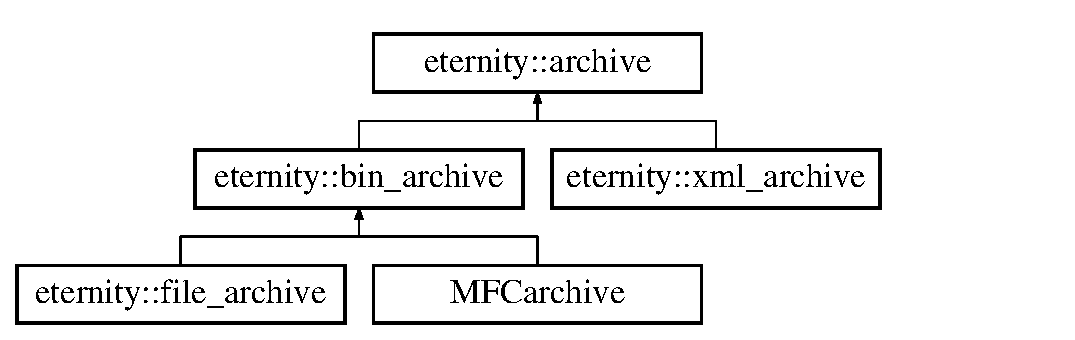
\includegraphics[height=3.000000cm]{classeternity_1_1archive}
\end{center}
\end{figure}
\subsection*{Public Types}
\begin{DoxyCompactItemize}
\item 
enum \hyperlink{classeternity_1_1archive_a8881f9ce8dbed2ee600c64b7925afef0}{opening\+\_\+mode} \{ \hyperlink{classeternity_1_1archive_a8881f9ce8dbed2ee600c64b7925afef0a5b952c27ebe4ca2612e939a1aa19baf5}{load}, 
\hyperlink{classeternity_1_1archive_a8881f9ce8dbed2ee600c64b7925afef0a06c18c297779389cb1cb03a2a7590ca8}{store}
 \}
\end{DoxyCompactItemize}
\subsection*{Public Member Functions}
\begin{DoxyCompactItemize}
\item 
\hyperlink{classeternity_1_1archive_adc5356f74fed2dd5daf230aa1ee6c58e}{archive} ()
\begin{DoxyCompactList}\small\item\em Simply the default constructor. \end{DoxyCompactList}\item 
void \hyperlink{classeternity_1_1archive_a941c3b590afc929089706b92ce4d5e13}{init} ()
\item 
int \hyperlink{classeternity_1_1archive_a2c4ab8d0935b130b38bce44f600bee99}{put\+\_\+pointer} (void $\ast$object)
\item 
bool \hyperlink{classeternity_1_1archive_a759dd5567021290542de13d090aa0963}{set\+\_\+loading} (bool val)
\begin{DoxyCompactList}\small\item\em Set the archive mode (loading or storing) \end{DoxyCompactList}\item 
bool \hyperlink{classeternity_1_1archive_af1ced5c2f5cd028d88033c40ac98cc71}{is\+\_\+loading} ()
\begin{DoxyCompactList}\small\item\em Verify the archive is in loading mode. \end{DoxyCompactList}\item 
bool \hyperlink{classeternity_1_1archive_afbd7e1d21409eae43622049624277405}{is\+\_\+storing} ()
\begin{DoxyCompactList}\small\item\em Verify the archive is in storing mode. \end{DoxyCompactList}\end{DoxyCompactItemize}
\subsection*{Protected Attributes}
\begin{DoxyCompactItemize}
\item 
bool \hyperlink{classeternity_1_1archive_a949b798deac030f2ab45ed54bf26dc4a}{m\+\_\+bloading}
\item 
std\+::vector$<$ void $\ast$ $>$ \hyperlink{classeternity_1_1archive_ae4a796ad260a0f581cf33be4f072d83a}{m\+\_\+v\+Pointerstored}
\end{DoxyCompactItemize}


\subsection{Detailed Description}
This class supply common services for all kind of persistence archives. The major one is the ability to stored doubled pointers only one time and so avoid circularity, broken links and lost spaces on hard disks. 

Definition at line 47 of file persist.\+hpp.



\subsection{Member Enumeration Documentation}
\mbox{\Hypertarget{classeternity_1_1archive_a8881f9ce8dbed2ee600c64b7925afef0}\label{classeternity_1_1archive_a8881f9ce8dbed2ee600c64b7925afef0}} 
\index{eternity\+::archive@{eternity\+::archive}!opening\+\_\+mode@{opening\+\_\+mode}}
\index{opening\+\_\+mode@{opening\+\_\+mode}!eternity\+::archive@{eternity\+::archive}}
\subsubsection{\texorpdfstring{opening\+\_\+mode}{opening\_mode}}
{\footnotesize\ttfamily enum \hyperlink{classeternity_1_1archive_a8881f9ce8dbed2ee600c64b7925afef0}{eternity\+::archive\+::opening\+\_\+mode}}

\begin{DoxyEnumFields}{Enumerator}
\raisebox{\heightof{T}}[0pt][0pt]{\index{load@{load}!eternity\+::archive@{eternity\+::archive}}\index{eternity\+::archive@{eternity\+::archive}!load@{load}}}\mbox{\Hypertarget{classeternity_1_1archive_a8881f9ce8dbed2ee600c64b7925afef0a5b952c27ebe4ca2612e939a1aa19baf5}\label{classeternity_1_1archive_a8881f9ce8dbed2ee600c64b7925afef0a5b952c27ebe4ca2612e939a1aa19baf5}} 
load&\\
\hline

\raisebox{\heightof{T}}[0pt][0pt]{\index{store@{store}!eternity\+::archive@{eternity\+::archive}}\index{eternity\+::archive@{eternity\+::archive}!store@{store}}}\mbox{\Hypertarget{classeternity_1_1archive_a8881f9ce8dbed2ee600c64b7925afef0a06c18c297779389cb1cb03a2a7590ca8}\label{classeternity_1_1archive_a8881f9ce8dbed2ee600c64b7925afef0a06c18c297779389cb1cb03a2a7590ca8}} 
store&\\
\hline

\end{DoxyEnumFields}


Definition at line 54 of file persist.\+hpp.



\subsection{Constructor \& Destructor Documentation}
\mbox{\Hypertarget{classeternity_1_1archive_adc5356f74fed2dd5daf230aa1ee6c58e}\label{classeternity_1_1archive_adc5356f74fed2dd5daf230aa1ee6c58e}} 
\index{eternity\+::archive@{eternity\+::archive}!archive@{archive}}
\index{archive@{archive}!eternity\+::archive@{eternity\+::archive}}
\subsubsection{\texorpdfstring{archive()}{archive()}}
{\footnotesize\ttfamily eternity\+::archive\+::archive (\begin{DoxyParamCaption}{ }\end{DoxyParamCaption})\hspace{0.3cm}{\ttfamily [inline]}}



Simply the default constructor. 



Definition at line 59 of file persist.\+hpp.



\subsection{Member Function Documentation}
\mbox{\Hypertarget{classeternity_1_1archive_a941c3b590afc929089706b92ce4d5e13}\label{classeternity_1_1archive_a941c3b590afc929089706b92ce4d5e13}} 
\index{eternity\+::archive@{eternity\+::archive}!init@{init}}
\index{init@{init}!eternity\+::archive@{eternity\+::archive}}
\subsubsection{\texorpdfstring{init()}{init()}}
{\footnotesize\ttfamily void eternity\+::archive\+::init (\begin{DoxyParamCaption}{ }\end{DoxyParamCaption})\hspace{0.3cm}{\ttfamily [inline]}}



Definition at line 62 of file persist.\+hpp.

\mbox{\Hypertarget{classeternity_1_1archive_af1ced5c2f5cd028d88033c40ac98cc71}\label{classeternity_1_1archive_af1ced5c2f5cd028d88033c40ac98cc71}} 
\index{eternity\+::archive@{eternity\+::archive}!is\+\_\+loading@{is\+\_\+loading}}
\index{is\+\_\+loading@{is\+\_\+loading}!eternity\+::archive@{eternity\+::archive}}
\subsubsection{\texorpdfstring{is\+\_\+loading()}{is\_loading()}}
{\footnotesize\ttfamily bool eternity\+::archive\+::is\+\_\+loading (\begin{DoxyParamCaption}{ }\end{DoxyParamCaption})\hspace{0.3cm}{\ttfamily [inline]}}



Verify the archive is in loading mode. 



Definition at line 80 of file persist.\+hpp.

\mbox{\Hypertarget{classeternity_1_1archive_afbd7e1d21409eae43622049624277405}\label{classeternity_1_1archive_afbd7e1d21409eae43622049624277405}} 
\index{eternity\+::archive@{eternity\+::archive}!is\+\_\+storing@{is\+\_\+storing}}
\index{is\+\_\+storing@{is\+\_\+storing}!eternity\+::archive@{eternity\+::archive}}
\subsubsection{\texorpdfstring{is\+\_\+storing()}{is\_storing()}}
{\footnotesize\ttfamily bool eternity\+::archive\+::is\+\_\+storing (\begin{DoxyParamCaption}{ }\end{DoxyParamCaption})\hspace{0.3cm}{\ttfamily [inline]}}



Verify the archive is in storing mode. 



Definition at line 85 of file persist.\+hpp.

\mbox{\Hypertarget{classeternity_1_1archive_a2c4ab8d0935b130b38bce44f600bee99}\label{classeternity_1_1archive_a2c4ab8d0935b130b38bce44f600bee99}} 
\index{eternity\+::archive@{eternity\+::archive}!put\+\_\+pointer@{put\+\_\+pointer}}
\index{put\+\_\+pointer@{put\+\_\+pointer}!eternity\+::archive@{eternity\+::archive}}
\subsubsection{\texorpdfstring{put\+\_\+pointer()}{put\_pointer()}}
{\footnotesize\ttfamily int eternity\+::archive\+::put\+\_\+pointer (\begin{DoxyParamCaption}\item[{void $\ast$}]{object }\end{DoxyParamCaption})}

Verify that object is stored only once. 

Definition at line 28 of file persist.\+cpp.

\mbox{\Hypertarget{classeternity_1_1archive_a759dd5567021290542de13d090aa0963}\label{classeternity_1_1archive_a759dd5567021290542de13d090aa0963}} 
\index{eternity\+::archive@{eternity\+::archive}!set\+\_\+loading@{set\+\_\+loading}}
\index{set\+\_\+loading@{set\+\_\+loading}!eternity\+::archive@{eternity\+::archive}}
\subsubsection{\texorpdfstring{set\+\_\+loading()}{set\_loading()}}
{\footnotesize\ttfamily bool eternity\+::archive\+::set\+\_\+loading (\begin{DoxyParamCaption}\item[{bool}]{val }\end{DoxyParamCaption})\hspace{0.3cm}{\ttfamily [inline]}}



Set the archive mode (loading or storing) 



Definition at line 75 of file persist.\+hpp.



\subsection{Member Data Documentation}
\mbox{\Hypertarget{classeternity_1_1archive_a949b798deac030f2ab45ed54bf26dc4a}\label{classeternity_1_1archive_a949b798deac030f2ab45ed54bf26dc4a}} 
\index{eternity\+::archive@{eternity\+::archive}!m\+\_\+bloading@{m\+\_\+bloading}}
\index{m\+\_\+bloading@{m\+\_\+bloading}!eternity\+::archive@{eternity\+::archive}}
\subsubsection{\texorpdfstring{m\+\_\+bloading}{m\_bloading}}
{\footnotesize\ttfamily bool eternity\+::archive\+::m\+\_\+bloading\hspace{0.3cm}{\ttfamily [protected]}}



Definition at line 49 of file persist.\+hpp.

\mbox{\Hypertarget{classeternity_1_1archive_ae4a796ad260a0f581cf33be4f072d83a}\label{classeternity_1_1archive_ae4a796ad260a0f581cf33be4f072d83a}} 
\index{eternity\+::archive@{eternity\+::archive}!m\+\_\+v\+Pointerstored@{m\+\_\+v\+Pointerstored}}
\index{m\+\_\+v\+Pointerstored@{m\+\_\+v\+Pointerstored}!eternity\+::archive@{eternity\+::archive}}
\subsubsection{\texorpdfstring{m\+\_\+v\+Pointerstored}{m\_vPointerstored}}
{\footnotesize\ttfamily std\+::vector$<$void$\ast$$>$ eternity\+::archive\+::m\+\_\+v\+Pointerstored\hspace{0.3cm}{\ttfamily [protected]}}



Definition at line 50 of file persist.\+hpp.



The documentation for this class was generated from the following files\+:\begin{DoxyCompactItemize}
\item 
/home/filip/\+Ph\+D/\+W\+D\+F\+Pipe\+\_\+test/p4\+T\+S\+A/include/eternity/\hyperlink{persist_8hpp}{persist.\+hpp}\item 
/home/filip/\+Ph\+D/\+W\+D\+F\+Pipe\+\_\+test/p4\+T\+S\+A/include/eternity/\hyperlink{persist_8cpp}{persist.\+cpp}\end{DoxyCompactItemize}

\hypertarget{classtsa_1_1_ar_durbin_estimator}{}\section{tsa\+:\+:Ar\+Durbin\+Estimator Class Reference}
\label{classtsa_1_1_ar_durbin_estimator}\index{tsa\+::\+Ar\+Durbin\+Estimator@{tsa\+::\+Ar\+Durbin\+Estimator}}


Estimate the AR coefficients and the P\+A\+R\+C\+OR of a time series using its correlation function.  




{\ttfamily \#include $<$Ar\+Durbin\+Estimator.\+hpp$>$}

Inheritance diagram for tsa\+:\+:Ar\+Durbin\+Estimator\+:\begin{figure}[H]
\begin{center}
\leavevmode
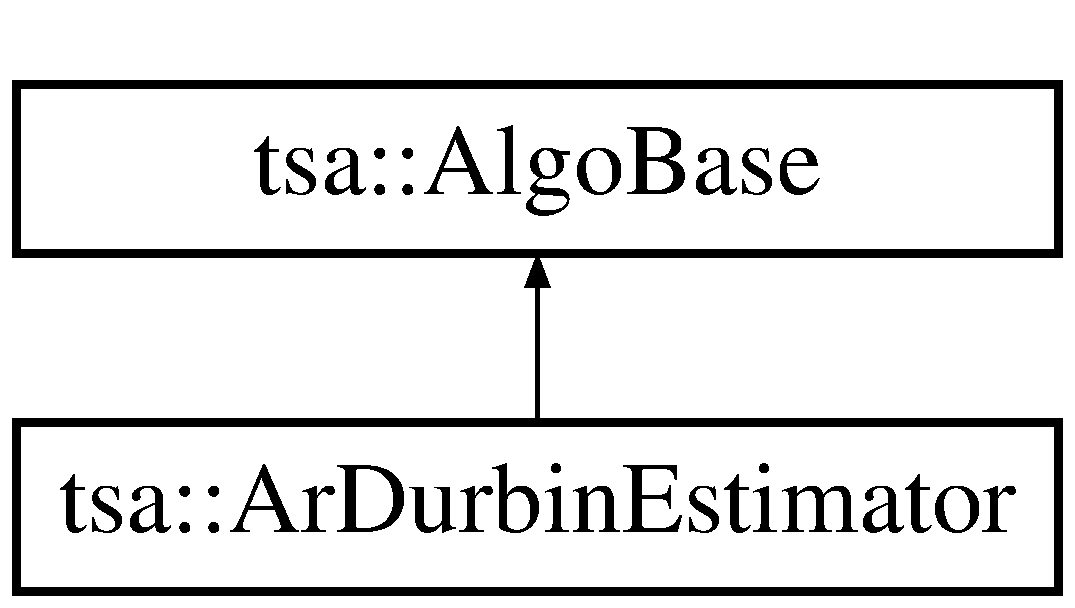
\includegraphics[height=2.000000cm]{classtsa_1_1_ar_durbin_estimator}
\end{center}
\end{figure}
\subsection*{Public Member Functions}
\begin{DoxyCompactItemize}
\item 
\hyperlink{classtsa_1_1_ar_durbin_estimator_a2c79884f3aca03b9f6701c826dcbc07b}{Ar\+Durbin\+Estimator} (unsigned int Ar\+Order)
\item 
virtual \hyperlink{classtsa_1_1_ar_durbin_estimator_a19ed9832b8899ebf095d339952ee0f47}{$\sim$\+Ar\+Durbin\+Estimator} ()
\end{DoxyCompactItemize}
\begin{Indent}\textbf{ Operations}\par
\begin{DoxyCompactItemize}
\item 
void \hyperlink{classtsa_1_1_ar_durbin_estimator_acefc1efc5c95e7b7b2703eab6aa0bcd6}{execute} (\hyperlink{namespacetsa_a8900fb03d849baf447a1a0efe2561fb2}{Dvector} \&Auto\+Corr, \hyperlink{namespacetsa_a8900fb03d849baf447a1a0efe2561fb2}{Dvector} \&Ar\+Parcor)
\end{DoxyCompactItemize}
\end{Indent}
\begin{Indent}\textbf{ Getters}\par
\begin{DoxyCompactItemize}
\item 
unsigned int \hyperlink{classtsa_1_1_ar_durbin_estimator_adce1261baa333e3a2c0c2c502544d135}{Get\+Ar\+Order} ()
\end{DoxyCompactItemize}
\end{Indent}
\begin{Indent}\textbf{ Setters}\par
\begin{DoxyCompactItemize}
\item 
void \hyperlink{classtsa_1_1_ar_durbin_estimator_af5cfeefd7e9a7bbd564373ead8d2a308}{Set\+Ar\+Order} (unsigned int P)
\end{DoxyCompactItemize}
\end{Indent}
\subsection*{Private Attributes}
\begin{DoxyCompactItemize}
\item 
unsigned int \hyperlink{classtsa_1_1_ar_durbin_estimator_a40783c942f77e9626e48eb1f8d7771ac}{m\+Ar\+Order}
\end{DoxyCompactItemize}


\subsection{Detailed Description}
Estimate the AR coefficients and the P\+A\+R\+C\+OR of a time series using its correlation function. 

Definition at line 78 of file Ar\+Durbin\+Estimator.\+hpp.



\subsection{Constructor \& Destructor Documentation}
\mbox{\Hypertarget{classtsa_1_1_ar_durbin_estimator_a2c79884f3aca03b9f6701c826dcbc07b}\label{classtsa_1_1_ar_durbin_estimator_a2c79884f3aca03b9f6701c826dcbc07b}} 
\index{tsa\+::\+Ar\+Durbin\+Estimator@{tsa\+::\+Ar\+Durbin\+Estimator}!Ar\+Durbin\+Estimator@{Ar\+Durbin\+Estimator}}
\index{Ar\+Durbin\+Estimator@{Ar\+Durbin\+Estimator}!tsa\+::\+Ar\+Durbin\+Estimator@{tsa\+::\+Ar\+Durbin\+Estimator}}
\subsubsection{\texorpdfstring{Ar\+Durbin\+Estimator()}{ArDurbinEstimator()}}
{\footnotesize\ttfamily tsa\+::\+Ar\+Durbin\+Estimator\+::\+Ar\+Durbin\+Estimator (\begin{DoxyParamCaption}\item[{unsigned int}]{Ar\+Order }\end{DoxyParamCaption})}

Constructor


\begin{DoxyParams}{Parameters}
{\em Ar\+Order} & order of the the AR model \\
\hline
\end{DoxyParams}


Definition at line 19 of file Ar\+Durbin\+Estimator.\+cpp.

\mbox{\Hypertarget{classtsa_1_1_ar_durbin_estimator_a19ed9832b8899ebf095d339952ee0f47}\label{classtsa_1_1_ar_durbin_estimator_a19ed9832b8899ebf095d339952ee0f47}} 
\index{tsa\+::\+Ar\+Durbin\+Estimator@{tsa\+::\+Ar\+Durbin\+Estimator}!````~Ar\+Durbin\+Estimator@{$\sim$\+Ar\+Durbin\+Estimator}}
\index{````~Ar\+Durbin\+Estimator@{$\sim$\+Ar\+Durbin\+Estimator}!tsa\+::\+Ar\+Durbin\+Estimator@{tsa\+::\+Ar\+Durbin\+Estimator}}
\subsubsection{\texorpdfstring{$\sim$\+Ar\+Durbin\+Estimator()}{~ArDurbinEstimator()}}
{\footnotesize\ttfamily tsa\+::\+Ar\+Durbin\+Estimator\+::$\sim$\+Ar\+Durbin\+Estimator (\begin{DoxyParamCaption}{ }\end{DoxyParamCaption})}

Destructor 

Definition at line 24 of file Ar\+Durbin\+Estimator.\+cpp.



\subsection{Member Function Documentation}
\mbox{\Hypertarget{classtsa_1_1_ar_durbin_estimator_acefc1efc5c95e7b7b2703eab6aa0bcd6}\label{classtsa_1_1_ar_durbin_estimator_acefc1efc5c95e7b7b2703eab6aa0bcd6}} 
\index{tsa\+::\+Ar\+Durbin\+Estimator@{tsa\+::\+Ar\+Durbin\+Estimator}!execute@{execute}}
\index{execute@{execute}!tsa\+::\+Ar\+Durbin\+Estimator@{tsa\+::\+Ar\+Durbin\+Estimator}}
\subsubsection{\texorpdfstring{execute()}{execute()}}
{\footnotesize\ttfamily void tsa\+::\+Ar\+Durbin\+Estimator\+::execute (\begin{DoxyParamCaption}\item[{\hyperlink{namespacetsa_a8900fb03d849baf447a1a0efe2561fb2}{Dvector} \&}]{Auto\+Corr,  }\item[{\hyperlink{namespacetsa_a8900fb03d849baf447a1a0efe2561fb2}{Dvector} \&}]{Ar\+Parcor }\end{DoxyParamCaption})}

The excute method estimate the AR and P\+A\+R\+C\+OR parameters with the Durbin rithm. \begin{DoxyPrecond}{Precondition}
The input of the algorithm must be the autocorrelation function in Toeplitz form
\end{DoxyPrecond}

\begin{DoxyParams}{Parameters}
{\em Auto\+Corr} & autocorrelation in Toeplitz form \\
\hline
{\em Ar\+Parcor} & vector containing the Reflection coefficients \\
\hline
\end{DoxyParams}
$<$ auxiliary matrix to estimate the AR coeff. by the Parcor

Estimation of the AR coefficient via durbin\textquotesingle{}s algorithm 

Definition at line 27 of file Ar\+Durbin\+Estimator.\+cpp.

\mbox{\Hypertarget{classtsa_1_1_ar_durbin_estimator_adce1261baa333e3a2c0c2c502544d135}\label{classtsa_1_1_ar_durbin_estimator_adce1261baa333e3a2c0c2c502544d135}} 
\index{tsa\+::\+Ar\+Durbin\+Estimator@{tsa\+::\+Ar\+Durbin\+Estimator}!Get\+Ar\+Order@{Get\+Ar\+Order}}
\index{Get\+Ar\+Order@{Get\+Ar\+Order}!tsa\+::\+Ar\+Durbin\+Estimator@{tsa\+::\+Ar\+Durbin\+Estimator}}
\subsubsection{\texorpdfstring{Get\+Ar\+Order()}{GetArOrder()}}
{\footnotesize\ttfamily unsigned int tsa\+::\+Ar\+Durbin\+Estimator\+::\+Get\+Ar\+Order (\begin{DoxyParamCaption}{ }\end{DoxyParamCaption})\hspace{0.3cm}{\ttfamily [inline]}}



Definition at line 117 of file Ar\+Durbin\+Estimator.\+hpp.

\mbox{\Hypertarget{classtsa_1_1_ar_durbin_estimator_af5cfeefd7e9a7bbd564373ead8d2a308}\label{classtsa_1_1_ar_durbin_estimator_af5cfeefd7e9a7bbd564373ead8d2a308}} 
\index{tsa\+::\+Ar\+Durbin\+Estimator@{tsa\+::\+Ar\+Durbin\+Estimator}!Set\+Ar\+Order@{Set\+Ar\+Order}}
\index{Set\+Ar\+Order@{Set\+Ar\+Order}!tsa\+::\+Ar\+Durbin\+Estimator@{tsa\+::\+Ar\+Durbin\+Estimator}}
\subsubsection{\texorpdfstring{Set\+Ar\+Order()}{SetArOrder()}}
{\footnotesize\ttfamily void tsa\+::\+Ar\+Durbin\+Estimator\+::\+Set\+Ar\+Order (\begin{DoxyParamCaption}\item[{unsigned int}]{P }\end{DoxyParamCaption})\hspace{0.3cm}{\ttfamily [inline]}}



Definition at line 128 of file Ar\+Durbin\+Estimator.\+hpp.



\subsection{Member Data Documentation}
\mbox{\Hypertarget{classtsa_1_1_ar_durbin_estimator_a40783c942f77e9626e48eb1f8d7771ac}\label{classtsa_1_1_ar_durbin_estimator_a40783c942f77e9626e48eb1f8d7771ac}} 
\index{tsa\+::\+Ar\+Durbin\+Estimator@{tsa\+::\+Ar\+Durbin\+Estimator}!m\+Ar\+Order@{m\+Ar\+Order}}
\index{m\+Ar\+Order@{m\+Ar\+Order}!tsa\+::\+Ar\+Durbin\+Estimator@{tsa\+::\+Ar\+Durbin\+Estimator}}
\subsubsection{\texorpdfstring{m\+Ar\+Order}{mArOrder}}
{\footnotesize\ttfamily unsigned int tsa\+::\+Ar\+Durbin\+Estimator\+::m\+Ar\+Order\hspace{0.3cm}{\ttfamily [private]}}



Definition at line 138 of file Ar\+Durbin\+Estimator.\+hpp.



The documentation for this class was generated from the following files\+:\begin{DoxyCompactItemize}
\item 
/home/filip/\+Ph\+D/\+W\+D\+F\+Pipe\+\_\+test/p4\+T\+S\+A/include/\hyperlink{_ar_durbin_estimator_8hpp}{Ar\+Durbin\+Estimator.\+hpp}\item 
/home/filip/\+Ph\+D/\+W\+D\+F\+Pipe\+\_\+test/p4\+T\+S\+A/src/\hyperlink{_ar_durbin_estimator_8cpp}{Ar\+Durbin\+Estimator.\+cpp}\end{DoxyCompactItemize}

\hypertarget{classtsa_1_1_arma2_psd}{}\section{tsa\+:\+:Arma2\+Psd Class Reference}
\label{classtsa_1_1_arma2_psd}\index{tsa\+::\+Arma2\+Psd@{tsa\+::\+Arma2\+Psd}}


Estimate the P\+SD for a A\+R\+MA model.  




{\ttfamily \#include $<$Arma2\+Psd.\+hpp$>$}

Inheritance diagram for tsa\+:\+:Arma2\+Psd\+:\begin{figure}[H]
\begin{center}
\leavevmode
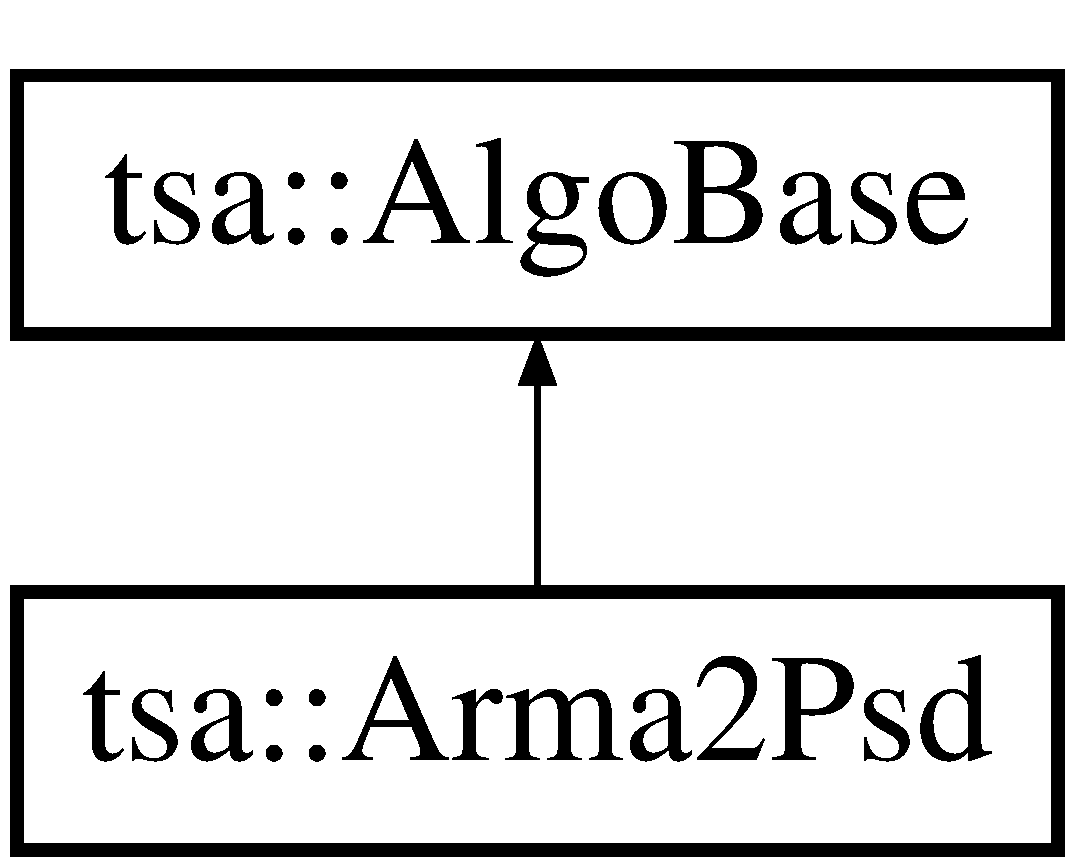
\includegraphics[height=2.000000cm]{classtsa_1_1_arma2_psd}
\end{center}
\end{figure}
\subsection*{Public Member Functions}
\begin{DoxyCompactItemize}
\item 
\hyperlink{classtsa_1_1_arma2_psd_a3488311932cc240d99a8e40c124da91d}{Arma2\+Psd} ()
\item 
\hyperlink{classtsa_1_1_arma2_psd_aa3a79a62709efcfdbb3268cf253837e1}{Arma2\+Psd} (const \hyperlink{classtsa_1_1_arma2_psd}{Arma2\+Psd} \&from)
\item 
virtual \hyperlink{classtsa_1_1_arma2_psd_aef3535e694289be52365ded1f83b7599}{$\sim$\+Arma2\+Psd} ()
\item 
\hyperlink{classtsa_1_1_arma2_psd}{Arma2\+Psd} \& \hyperlink{classtsa_1_1_arma2_psd_a85b4577ccb8331c63c004eb2e917b59b}{operator=} (const \hyperlink{classtsa_1_1_arma2_psd}{Arma2\+Psd} \&from)
\end{DoxyCompactItemize}
\begin{Indent}\textbf{ Operations}\par
\begin{DoxyCompactItemize}
\item 
void \hyperlink{classtsa_1_1_arma2_psd_a345f2bf999cad8a585d7fff389bbefa4}{operator()} (\hyperlink{classtsa_1_1_a_r_m_a_view}{A\+R\+M\+A\+View} \&arma, \hyperlink{namespacetsa_ac599574bcc094eda25613724b8f3ca9e}{Seq\+View\+Double} \&Psd)
\item 
void \hyperlink{classtsa_1_1_arma2_psd_afb147e11ba8e3ddef347fdf121cac5e1}{execute} (\hyperlink{namespacetsa_a8900fb03d849baf447a1a0efe2561fb2}{Dvector} \&AR, \hyperlink{namespacetsa_a8900fb03d849baf447a1a0efe2561fb2}{Dvector} \&MA, \hyperlink{namespacetsa_a8900fb03d849baf447a1a0efe2561fb2}{Dvector} \&psd)
\begin{DoxyCompactList}\small\item\em Estimate the P\+SD for a A\+R\+MA model. \end{DoxyCompactList}\end{DoxyCompactItemize}
\end{Indent}


\subsection{Detailed Description}
Estimate the P\+SD for a A\+R\+MA model. 

Definition at line 72 of file Arma2\+Psd.\+hpp.



\subsection{Constructor \& Destructor Documentation}
\mbox{\Hypertarget{classtsa_1_1_arma2_psd_a3488311932cc240d99a8e40c124da91d}\label{classtsa_1_1_arma2_psd_a3488311932cc240d99a8e40c124da91d}} 
\index{tsa\+::\+Arma2\+Psd@{tsa\+::\+Arma2\+Psd}!Arma2\+Psd@{Arma2\+Psd}}
\index{Arma2\+Psd@{Arma2\+Psd}!tsa\+::\+Arma2\+Psd@{tsa\+::\+Arma2\+Psd}}
\subsubsection{\texorpdfstring{Arma2\+Psd()}{Arma2Psd()}\hspace{0.1cm}{\footnotesize\ttfamily [1/2]}}
{\footnotesize\ttfamily tsa\+::\+Arma2\+Psd\+::\+Arma2\+Psd (\begin{DoxyParamCaption}{ }\end{DoxyParamCaption})}

Constructor 

Definition at line 19 of file Arma2\+Psd.\+cpp.

\mbox{\Hypertarget{classtsa_1_1_arma2_psd_aa3a79a62709efcfdbb3268cf253837e1}\label{classtsa_1_1_arma2_psd_aa3a79a62709efcfdbb3268cf253837e1}} 
\index{tsa\+::\+Arma2\+Psd@{tsa\+::\+Arma2\+Psd}!Arma2\+Psd@{Arma2\+Psd}}
\index{Arma2\+Psd@{Arma2\+Psd}!tsa\+::\+Arma2\+Psd@{tsa\+::\+Arma2\+Psd}}
\subsubsection{\texorpdfstring{Arma2\+Psd()}{Arma2Psd()}\hspace{0.1cm}{\footnotesize\ttfamily [2/2]}}
{\footnotesize\ttfamily tsa\+::\+Arma2\+Psd\+::\+Arma2\+Psd (\begin{DoxyParamCaption}\item[{const \hyperlink{classtsa_1_1_arma2_psd}{Arma2\+Psd} \&}]{from }\end{DoxyParamCaption})}

Copy constructor


\begin{DoxyParams}{Parameters}
{\em from} & The instance that must be copied \\
\hline
\end{DoxyParams}


Definition at line 26 of file Arma2\+Psd.\+cpp.

\mbox{\Hypertarget{classtsa_1_1_arma2_psd_aef3535e694289be52365ded1f83b7599}\label{classtsa_1_1_arma2_psd_aef3535e694289be52365ded1f83b7599}} 
\index{tsa\+::\+Arma2\+Psd@{tsa\+::\+Arma2\+Psd}!````~Arma2\+Psd@{$\sim$\+Arma2\+Psd}}
\index{````~Arma2\+Psd@{$\sim$\+Arma2\+Psd}!tsa\+::\+Arma2\+Psd@{tsa\+::\+Arma2\+Psd}}
\subsubsection{\texorpdfstring{$\sim$\+Arma2\+Psd()}{~Arma2Psd()}}
{\footnotesize\ttfamily tsa\+::\+Arma2\+Psd\+::$\sim$\+Arma2\+Psd (\begin{DoxyParamCaption}{ }\end{DoxyParamCaption})\hspace{0.3cm}{\ttfamily [virtual]}}

Destructor 

Definition at line 34 of file Arma2\+Psd.\+cpp.



\subsection{Member Function Documentation}
\mbox{\Hypertarget{classtsa_1_1_arma2_psd_afb147e11ba8e3ddef347fdf121cac5e1}\label{classtsa_1_1_arma2_psd_afb147e11ba8e3ddef347fdf121cac5e1}} 
\index{tsa\+::\+Arma2\+Psd@{tsa\+::\+Arma2\+Psd}!execute@{execute}}
\index{execute@{execute}!tsa\+::\+Arma2\+Psd@{tsa\+::\+Arma2\+Psd}}
\subsubsection{\texorpdfstring{execute()}{execute()}}
{\footnotesize\ttfamily void tsa\+::\+Arma2\+Psd\+::execute (\begin{DoxyParamCaption}\item[{\hyperlink{namespacetsa_a8900fb03d849baf447a1a0efe2561fb2}{Dvector} \&}]{AR,  }\item[{\hyperlink{namespacetsa_a8900fb03d849baf447a1a0efe2561fb2}{Dvector} \&}]{MA,  }\item[{\hyperlink{namespacetsa_a8900fb03d849baf447a1a0efe2561fb2}{Dvector} \&}]{psd }\end{DoxyParamCaption})}



Estimate the P\+SD for a A\+R\+MA model. 

It has been implemented a fast recurrence algorithm fot the estimation of sin and cos, by A. Vicere\textquotesingle{}.


\begin{DoxyParams}{Parameters}
{\em AR} & the autoregressive part \\
\hline
{\em MA} & the moving average aprt \\
\hline
{\em psd} & the Power Spectral Density \\
\hline
\end{DoxyParams}


Definition at line 78 of file Arma2\+Psd.\+cpp.

\mbox{\Hypertarget{classtsa_1_1_arma2_psd_a345f2bf999cad8a585d7fff389bbefa4}\label{classtsa_1_1_arma2_psd_a345f2bf999cad8a585d7fff389bbefa4}} 
\index{tsa\+::\+Arma2\+Psd@{tsa\+::\+Arma2\+Psd}!operator()@{operator()}}
\index{operator()@{operator()}!tsa\+::\+Arma2\+Psd@{tsa\+::\+Arma2\+Psd}}
\subsubsection{\texorpdfstring{operator()()}{operator()()}}
{\footnotesize\ttfamily void tsa\+::\+Arma2\+Psd\+::operator() (\begin{DoxyParamCaption}\item[{\hyperlink{classtsa_1_1_a_r_m_a_view}{A\+R\+M\+A\+View} \&}]{arma,  }\item[{\hyperlink{namespacetsa_ac599574bcc094eda25613724b8f3ca9e}{Seq\+View\+Double} \&}]{Psd }\end{DoxyParamCaption})}

\begin{DoxyPrecond}{Precondition}
The P or the Q order must be greater than 0
\end{DoxyPrecond}

\begin{DoxyParams}{Parameters}
{\em arma} & the Arma View\\
\hline
\end{DoxyParams}
\begin{DoxyReturn}{Returns}
Psd the Power Spectral density 
\end{DoxyReturn}


Definition at line 49 of file Arma2\+Psd.\+cpp.

\mbox{\Hypertarget{classtsa_1_1_arma2_psd_a85b4577ccb8331c63c004eb2e917b59b}\label{classtsa_1_1_arma2_psd_a85b4577ccb8331c63c004eb2e917b59b}} 
\index{tsa\+::\+Arma2\+Psd@{tsa\+::\+Arma2\+Psd}!operator=@{operator=}}
\index{operator=@{operator=}!tsa\+::\+Arma2\+Psd@{tsa\+::\+Arma2\+Psd}}
\subsubsection{\texorpdfstring{operator=()}{operator=()}}
{\footnotesize\ttfamily \hyperlink{classtsa_1_1_arma2_psd}{Arma2\+Psd} \& tsa\+::\+Arma2\+Psd\+::operator= (\begin{DoxyParamCaption}\item[{const \hyperlink{classtsa_1_1_arma2_psd}{Arma2\+Psd} \&}]{from }\end{DoxyParamCaption})}

Assignement operator


\begin{DoxyParams}{Parameters}
{\em from} & The instance to be assigned from\\
\hline
\end{DoxyParams}
\begin{DoxyReturn}{Returns}
a reference to a new object 
\end{DoxyReturn}


Definition at line 45 of file Arma2\+Psd.\+cpp.



The documentation for this class was generated from the following files\+:\begin{DoxyCompactItemize}
\item 
/home/filip/\+Ph\+D/\+W\+D\+F\+Pipe\+\_\+test/p4\+T\+S\+A/include/\hyperlink{_arma2_psd_8hpp}{Arma2\+Psd.\+hpp}\item 
/home/filip/\+Ph\+D/\+W\+D\+F\+Pipe\+\_\+test/p4\+T\+S\+A/src/\hyperlink{_arma2_psd_8cpp}{Arma2\+Psd.\+cpp}\end{DoxyCompactItemize}

\hypertarget{classtsa_1_1_arma2_t_f}{}\section{tsa\+:\+:Arma2\+TF Class Reference}
\label{classtsa_1_1_arma2_t_f}\index{tsa\+::\+Arma2\+TF@{tsa\+::\+Arma2\+TF}}


Estimate the Transfer function using the A\+R\+MA parametrization.  




{\ttfamily \#include $<$Arma2\+T\+F.\+hpp$>$}

Inheritance diagram for tsa\+:\+:Arma2\+TF\+:\begin{figure}[H]
\begin{center}
\leavevmode
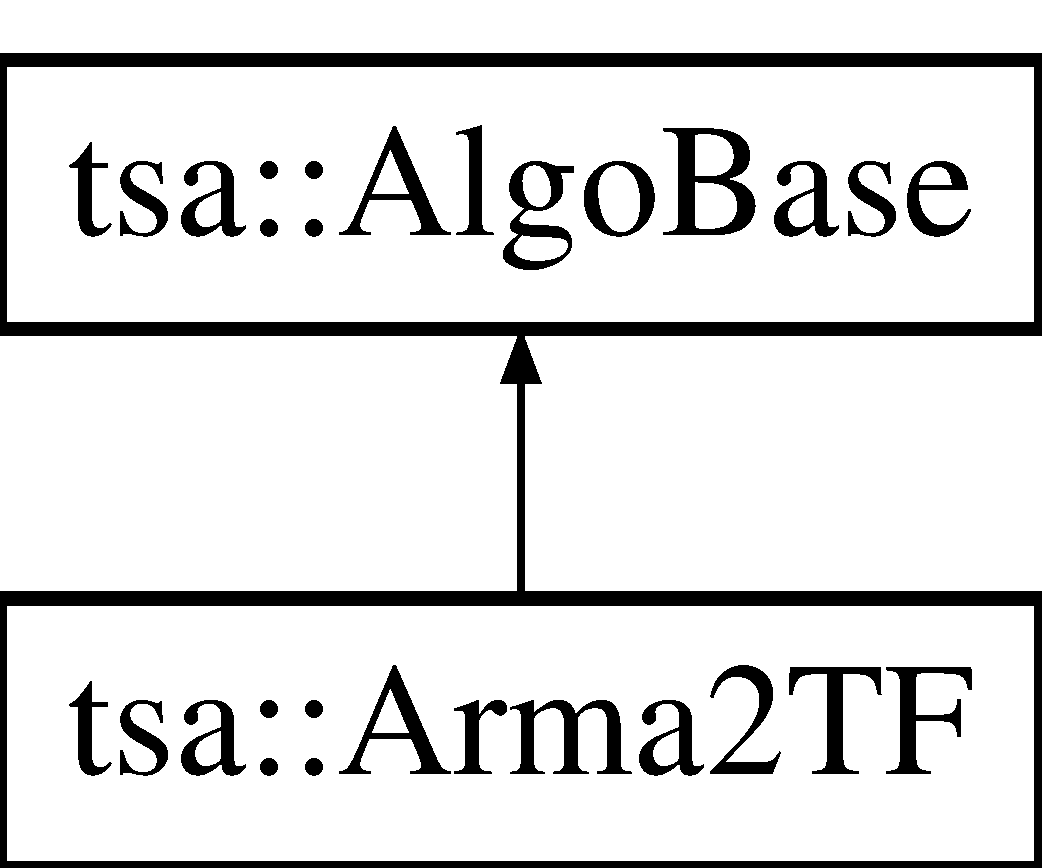
\includegraphics[height=2.000000cm]{classtsa_1_1_arma2_t_f}
\end{center}
\end{figure}
\subsection*{Public Member Functions}
\begin{DoxyCompactItemize}
\item 
\hyperlink{classtsa_1_1_arma2_t_f_aabbe1c03f711805d11bf7f4951149617}{Arma2\+TF} ()
\item 
\hyperlink{classtsa_1_1_arma2_t_f_a93ac79691dd4f811d21f2021476ce4b5}{Arma2\+TF} (const \hyperlink{classtsa_1_1_arma2_t_f}{Arma2\+TF} \&from)
\item 
virtual \hyperlink{classtsa_1_1_arma2_t_f_aa48720a5c5a48ebfbaf1ee080f27a411}{$\sim$\+Arma2\+TF} ()
\item 
\hyperlink{classtsa_1_1_arma2_t_f}{Arma2\+TF} \& \hyperlink{classtsa_1_1_arma2_t_f_ac2fa5584ff0fed36eabfc908ded9b5de}{operator=} (const \hyperlink{classtsa_1_1_arma2_t_f}{Arma2\+TF} \&from)
\end{DoxyCompactItemize}
\begin{Indent}\textbf{ Operations}\par
\begin{DoxyCompactItemize}
\item 
void \hyperlink{classtsa_1_1_arma2_t_f_ab1e6a1c801109ef7f884317bacbe5f64}{operator()} (\hyperlink{classtsa_1_1_a_r_m_a_view}{A\+R\+M\+A\+View} \&arma, \hyperlink{namespacetsa_ab32775c889b53c40fa83939f22372b75}{Seq\+View\+Complex} \&TF)
\begin{DoxyCompactList}\small\item\em Brief documentation for the execute method. \end{DoxyCompactList}\item 
void \hyperlink{classtsa_1_1_arma2_t_f_ad7716bcd575670622bdec2fc32745e6e}{execute} (\hyperlink{namespacetsa_a8900fb03d849baf447a1a0efe2561fb2}{Dvector} \&AR, \hyperlink{namespacetsa_a8900fb03d849baf447a1a0efe2561fb2}{Dvector} \&MA, \hyperlink{namespacetsa_a054d1045ead95a65819e9e5722baf600}{Cvector} \&TF)
\end{DoxyCompactItemize}
\end{Indent}


\subsection{Detailed Description}
Estimate the Transfer function using the A\+R\+MA parametrization. 

Definition at line 75 of file Arma2\+T\+F.\+hpp.



\subsection{Constructor \& Destructor Documentation}
\mbox{\Hypertarget{classtsa_1_1_arma2_t_f_aabbe1c03f711805d11bf7f4951149617}\label{classtsa_1_1_arma2_t_f_aabbe1c03f711805d11bf7f4951149617}} 
\index{tsa\+::\+Arma2\+TF@{tsa\+::\+Arma2\+TF}!Arma2\+TF@{Arma2\+TF}}
\index{Arma2\+TF@{Arma2\+TF}!tsa\+::\+Arma2\+TF@{tsa\+::\+Arma2\+TF}}
\subsubsection{\texorpdfstring{Arma2\+T\+F()}{Arma2TF()}\hspace{0.1cm}{\footnotesize\ttfamily [1/2]}}
{\footnotesize\ttfamily tsa\+::\+Arma2\+T\+F\+::\+Arma2\+TF (\begin{DoxyParamCaption}{ }\end{DoxyParamCaption})}

Constructor 

Definition at line 19 of file Arma2\+T\+F.\+cpp.

\mbox{\Hypertarget{classtsa_1_1_arma2_t_f_a93ac79691dd4f811d21f2021476ce4b5}\label{classtsa_1_1_arma2_t_f_a93ac79691dd4f811d21f2021476ce4b5}} 
\index{tsa\+::\+Arma2\+TF@{tsa\+::\+Arma2\+TF}!Arma2\+TF@{Arma2\+TF}}
\index{Arma2\+TF@{Arma2\+TF}!tsa\+::\+Arma2\+TF@{tsa\+::\+Arma2\+TF}}
\subsubsection{\texorpdfstring{Arma2\+T\+F()}{Arma2TF()}\hspace{0.1cm}{\footnotesize\ttfamily [2/2]}}
{\footnotesize\ttfamily tsa\+::\+Arma2\+T\+F\+::\+Arma2\+TF (\begin{DoxyParamCaption}\item[{const \hyperlink{classtsa_1_1_arma2_t_f}{Arma2\+TF} \&}]{from }\end{DoxyParamCaption})}

Copy constructor


\begin{DoxyParams}{Parameters}
{\em from} & The instance that must be copied \\
\hline
\end{DoxyParams}


Definition at line 109 of file Arma2\+T\+F.\+cpp.

\mbox{\Hypertarget{classtsa_1_1_arma2_t_f_aa48720a5c5a48ebfbaf1ee080f27a411}\label{classtsa_1_1_arma2_t_f_aa48720a5c5a48ebfbaf1ee080f27a411}} 
\index{tsa\+::\+Arma2\+TF@{tsa\+::\+Arma2\+TF}!````~Arma2\+TF@{$\sim$\+Arma2\+TF}}
\index{````~Arma2\+TF@{$\sim$\+Arma2\+TF}!tsa\+::\+Arma2\+TF@{tsa\+::\+Arma2\+TF}}
\subsubsection{\texorpdfstring{$\sim$\+Arma2\+T\+F()}{~Arma2TF()}}
{\footnotesize\ttfamily tsa\+::\+Arma2\+T\+F\+::$\sim$\+Arma2\+TF (\begin{DoxyParamCaption}{ }\end{DoxyParamCaption})\hspace{0.3cm}{\ttfamily [virtual]}}

Destructor 

Definition at line 117 of file Arma2\+T\+F.\+cpp.



\subsection{Member Function Documentation}
\mbox{\Hypertarget{classtsa_1_1_arma2_t_f_ad7716bcd575670622bdec2fc32745e6e}\label{classtsa_1_1_arma2_t_f_ad7716bcd575670622bdec2fc32745e6e}} 
\index{tsa\+::\+Arma2\+TF@{tsa\+::\+Arma2\+TF}!execute@{execute}}
\index{execute@{execute}!tsa\+::\+Arma2\+TF@{tsa\+::\+Arma2\+TF}}
\subsubsection{\texorpdfstring{execute()}{execute()}}
{\footnotesize\ttfamily void tsa\+::\+Arma2\+T\+F\+::execute (\begin{DoxyParamCaption}\item[{\hyperlink{namespacetsa_a8900fb03d849baf447a1a0efe2561fb2}{Dvector} \&}]{AR,  }\item[{\hyperlink{namespacetsa_a8900fb03d849baf447a1a0efe2561fb2}{Dvector} \&}]{MA,  }\item[{\hyperlink{namespacetsa_a054d1045ead95a65819e9e5722baf600}{Cvector} \&}]{TF }\end{DoxyParamCaption})}

Declaration of execute operation


\begin{DoxyParams}{Parameters}
{\em AR} & autoregressive part \\
\hline
{\em MA} & moving average part \\
\hline
{\em TF} & transfer function \\
\hline
\end{DoxyParams}


Definition at line 59 of file Arma2\+T\+F.\+cpp.

\mbox{\Hypertarget{classtsa_1_1_arma2_t_f_ab1e6a1c801109ef7f884317bacbe5f64}\label{classtsa_1_1_arma2_t_f_ab1e6a1c801109ef7f884317bacbe5f64}} 
\index{tsa\+::\+Arma2\+TF@{tsa\+::\+Arma2\+TF}!operator()@{operator()}}
\index{operator()@{operator()}!tsa\+::\+Arma2\+TF@{tsa\+::\+Arma2\+TF}}
\subsubsection{\texorpdfstring{operator()()}{operator()()}}
{\footnotesize\ttfamily void tsa\+::\+Arma2\+T\+F\+::operator() (\begin{DoxyParamCaption}\item[{\hyperlink{classtsa_1_1_a_r_m_a_view}{A\+R\+M\+A\+View} \&}]{arma,  }\item[{\hyperlink{namespacetsa_ab32775c889b53c40fa83939f22372b75}{Seq\+View\+Complex} \&}]{TF }\end{DoxyParamCaption})}



Brief documentation for the execute method. 

Start of the long documentation for execute method.

\begin{DoxyPrecond}{Precondition}
A precondition 
\end{DoxyPrecond}
\begin{DoxyPostcond}{Postcondition}
A postcondition 
\end{DoxyPostcond}

\begin{DoxyExceptions}{Exceptions}
{\em An} & exception\\
\hline
\end{DoxyExceptions}

\begin{DoxyParams}{Parameters}
{\em a} & parameter\\
\hline
\end{DoxyParams}
\begin{DoxyReturn}{Returns}
a returned value 
\end{DoxyReturn}
\begin{DoxyRefDesc}{Todo}
\item[\hyperlink{todo__todo000001}{Todo}]implement Multivectorial Arma \end{DoxyRefDesc}


Definition at line 23 of file Arma2\+T\+F.\+cpp.

\mbox{\Hypertarget{classtsa_1_1_arma2_t_f_ac2fa5584ff0fed36eabfc908ded9b5de}\label{classtsa_1_1_arma2_t_f_ac2fa5584ff0fed36eabfc908ded9b5de}} 
\index{tsa\+::\+Arma2\+TF@{tsa\+::\+Arma2\+TF}!operator=@{operator=}}
\index{operator=@{operator=}!tsa\+::\+Arma2\+TF@{tsa\+::\+Arma2\+TF}}
\subsubsection{\texorpdfstring{operator=()}{operator=()}}
{\footnotesize\ttfamily \hyperlink{classtsa_1_1_arma2_t_f}{Arma2\+TF} \& tsa\+::\+Arma2\+T\+F\+::operator= (\begin{DoxyParamCaption}\item[{const \hyperlink{classtsa_1_1_arma2_t_f}{Arma2\+TF} \&}]{from }\end{DoxyParamCaption})}

Assignement operator


\begin{DoxyParams}{Parameters}
{\em from} & The instance to be assigned from\\
\hline
\end{DoxyParams}
\begin{DoxyReturn}{Returns}
a reference to a new object 
\end{DoxyReturn}


Definition at line 127 of file Arma2\+T\+F.\+cpp.



The documentation for this class was generated from the following files\+:\begin{DoxyCompactItemize}
\item 
/home/filip/\+Ph\+D/\+W\+D\+F\+Pipe\+\_\+test/p4\+T\+S\+A/include/\hyperlink{_arma2_t_f_8hpp}{Arma2\+T\+F.\+hpp}\item 
/home/filip/\+Ph\+D/\+W\+D\+F\+Pipe\+\_\+test/p4\+T\+S\+A/src/\hyperlink{_arma2_t_f_8cpp}{Arma2\+T\+F.\+cpp}\end{DoxyCompactItemize}

\hypertarget{classtsa_1_1_a_r_m_a_filter}{}\section{tsa\+:\+:A\+R\+M\+A\+Filter Class Reference}
\label{classtsa_1_1_a_r_m_a_filter}\index{tsa\+::\+A\+R\+M\+A\+Filter@{tsa\+::\+A\+R\+M\+A\+Filter}}


Implement the A\+R\+MA filtering.  




{\ttfamily \#include $<$A\+R\+M\+A\+Filter.\+hpp$>$}

Inheritance diagram for tsa\+:\+:A\+R\+M\+A\+Filter\+:\begin{figure}[H]
\begin{center}
\leavevmode
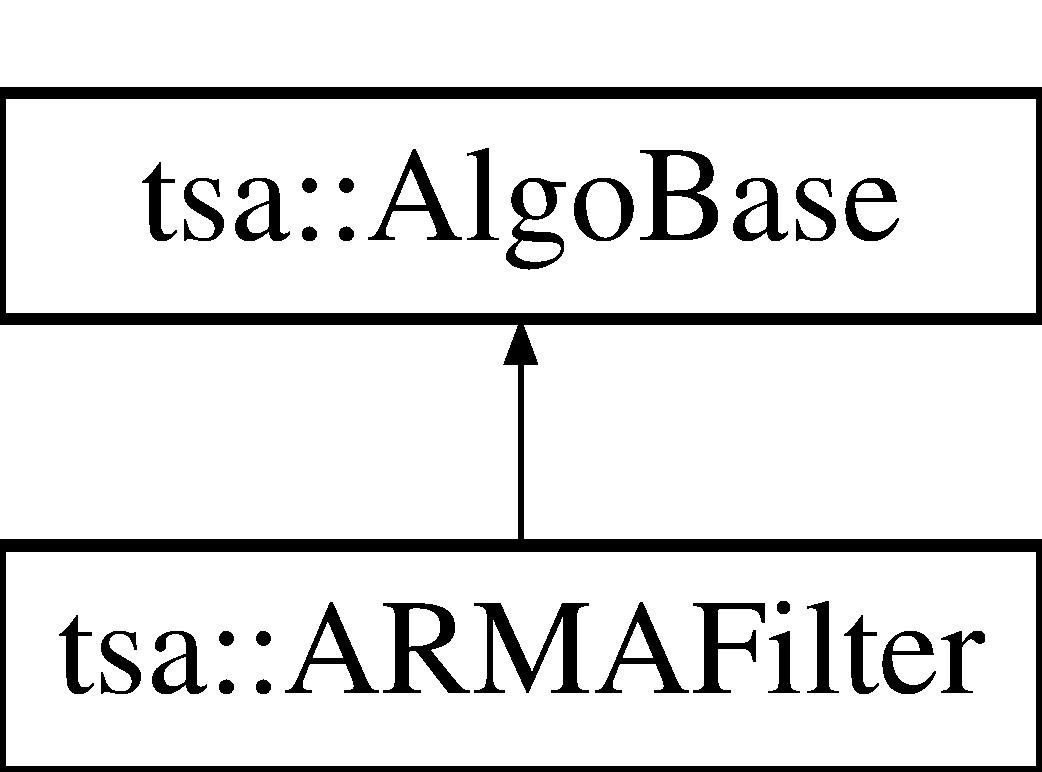
\includegraphics[height=2.000000cm]{classtsa_1_1_a_r_m_a_filter}
\end{center}
\end{figure}
\subsection*{Public Member Functions}
\begin{DoxyCompactItemize}
\item 
\hyperlink{classtsa_1_1_a_r_m_a_filter_acfa4406559bb327a4bfd5139db46f941}{A\+R\+M\+A\+Filter} (const std\+::vector$<$ double $>$ \&\hyperlink{classtsa_1_1_a_r_m_a_filter_abadc75a208b4e28e28e7341c6bbfbbce}{m\+AR}, const std\+::vector$<$ double $>$ \&\hyperlink{classtsa_1_1_a_r_m_a_filter_aa4b780d4db5a5c5326e92f1c766613fb}{m\+MA}, double gain)
\item 
virtual \hyperlink{classtsa_1_1_a_r_m_a_filter_affe37273b08f1c5f21a9d11170f1a119}{$\sim$\+A\+R\+M\+A\+Filter} ()
\end{DoxyCompactItemize}
\begin{Indent}\textbf{ Operations}\par
\begin{DoxyCompactItemize}
\item 
void \hyperlink{classtsa_1_1_a_r_m_a_filter_af5ff08e872b2cbb13221c8e90158c3a3}{operator()} (\hyperlink{namespacetsa_ac599574bcc094eda25613724b8f3ca9e}{Seq\+View\+Double} \&in, \hyperlink{namespacetsa_ac599574bcc094eda25613724b8f3ca9e}{Seq\+View\+Double} \&out)
\item 
void \hyperlink{classtsa_1_1_a_r_m_a_filter_a9c0be1ce8ede64c97bc2845423d7380f}{execute} (\hyperlink{namespacetsa_ad260cd21c1891c4ed391fe788569aba4}{Dmatrix} \&in, \hyperlink{namespacetsa_ad260cd21c1891c4ed391fe788569aba4}{Dmatrix} \&out, double scale)
\end{DoxyCompactItemize}
\end{Indent}
\begin{Indent}\textbf{ Setters}\par
\begin{DoxyCompactItemize}
\item 
void \hyperlink{classtsa_1_1_a_r_m_a_filter_a4665d54649f2e971303429dea11a6ae5}{Set\+Filter} (const std\+::vector$<$ double $>$ \&\hyperlink{classtsa_1_1_a_r_m_a_filter_abadc75a208b4e28e28e7341c6bbfbbce}{m\+AR}, const std\+::vector$<$ double $>$ \&\hyperlink{classtsa_1_1_a_r_m_a_filter_aa4b780d4db5a5c5326e92f1c766613fb}{m\+MA}, double gain)
\end{DoxyCompactItemize}
\end{Indent}
\subsection*{Private Attributes}
\begin{DoxyCompactItemize}
\item 
\hyperlink{namespacetsa_ad1e65e148c1b8be13ee4da5b246b5adf}{L\+Dvector} \hyperlink{classtsa_1_1_a_r_m_a_filter_abadc75a208b4e28e28e7341c6bbfbbce}{m\+AR}
\item 
\hyperlink{namespacetsa_ad1e65e148c1b8be13ee4da5b246b5adf}{L\+Dvector} \hyperlink{classtsa_1_1_a_r_m_a_filter_aa4b780d4db5a5c5326e92f1c766613fb}{m\+MA}
\item 
long double \hyperlink{classtsa_1_1_a_r_m_a_filter_abb62dc2fe30975bb49e0105915143169}{m\+Gain}
\item 
int \hyperlink{classtsa_1_1_a_r_m_a_filter_a12aaa04dea7ac6d48c99c66319286ae4}{m\+In\+Pointer}
\item 
int \hyperlink{classtsa_1_1_a_r_m_a_filter_a223497bf7eb2f652a8c776f67837e6e9}{m\+Out\+Pointer}
\item 
\hyperlink{namespacetsa_ad1e65e148c1b8be13ee4da5b246b5adf}{L\+Dvector} \hyperlink{classtsa_1_1_a_r_m_a_filter_aa8de4abbeb3ed3078a7e9f1440619ac1}{m\+In\+Buffer}
\item 
\hyperlink{namespacetsa_ad1e65e148c1b8be13ee4da5b246b5adf}{L\+Dvector} \hyperlink{classtsa_1_1_a_r_m_a_filter_a45a752b94a28a77c8269bee486d0c85c}{m\+Out\+Buffer}
\end{DoxyCompactItemize}


\subsection{Detailed Description}
Implement the A\+R\+MA filtering. 

This class implement a general A\+R\+MA filter. Given an input sequence x(n) and an output sequence y(n) an A\+R\+MA filter is defined by the relation (look at the signs definitions..)

a(0) y(n) = a(1) y(n-\/1) + ... + a(\+N) y(n-\/N) + b(0) x(n) + b(1) x(n-\/1) + .... + b(\+M) x(n-\/M) 

Definition at line 78 of file A\+R\+M\+A\+Filter.\+hpp.



\subsection{Constructor \& Destructor Documentation}
\mbox{\Hypertarget{classtsa_1_1_a_r_m_a_filter_acfa4406559bb327a4bfd5139db46f941}\label{classtsa_1_1_a_r_m_a_filter_acfa4406559bb327a4bfd5139db46f941}} 
\index{tsa\+::\+A\+R\+M\+A\+Filter@{tsa\+::\+A\+R\+M\+A\+Filter}!A\+R\+M\+A\+Filter@{A\+R\+M\+A\+Filter}}
\index{A\+R\+M\+A\+Filter@{A\+R\+M\+A\+Filter}!tsa\+::\+A\+R\+M\+A\+Filter@{tsa\+::\+A\+R\+M\+A\+Filter}}
\subsubsection{\texorpdfstring{A\+R\+M\+A\+Filter()}{ARMAFilter()}}
{\footnotesize\ttfamily tsa\+::\+A\+R\+M\+A\+Filter\+::\+A\+R\+M\+A\+Filter (\begin{DoxyParamCaption}\item[{const std\+::vector$<$ double $>$ \&}]{m\+AR,  }\item[{const std\+::vector$<$ double $>$ \&}]{m\+MA,  }\item[{double}]{gain }\end{DoxyParamCaption})}

Constructor 

Definition at line 5 of file A\+R\+M\+A\+Filter.\+cpp.

\mbox{\Hypertarget{classtsa_1_1_a_r_m_a_filter_affe37273b08f1c5f21a9d11170f1a119}\label{classtsa_1_1_a_r_m_a_filter_affe37273b08f1c5f21a9d11170f1a119}} 
\index{tsa\+::\+A\+R\+M\+A\+Filter@{tsa\+::\+A\+R\+M\+A\+Filter}!````~A\+R\+M\+A\+Filter@{$\sim$\+A\+R\+M\+A\+Filter}}
\index{````~A\+R\+M\+A\+Filter@{$\sim$\+A\+R\+M\+A\+Filter}!tsa\+::\+A\+R\+M\+A\+Filter@{tsa\+::\+A\+R\+M\+A\+Filter}}
\subsubsection{\texorpdfstring{$\sim$\+A\+R\+M\+A\+Filter()}{~ARMAFilter()}}
{\footnotesize\ttfamily tsa\+::\+A\+R\+M\+A\+Filter\+::$\sim$\+A\+R\+M\+A\+Filter (\begin{DoxyParamCaption}{ }\end{DoxyParamCaption})\hspace{0.3cm}{\ttfamily [virtual]}}

Destructor 

Definition at line 27 of file A\+R\+M\+A\+Filter.\+cpp.



\subsection{Member Function Documentation}
\mbox{\Hypertarget{classtsa_1_1_a_r_m_a_filter_a9c0be1ce8ede64c97bc2845423d7380f}\label{classtsa_1_1_a_r_m_a_filter_a9c0be1ce8ede64c97bc2845423d7380f}} 
\index{tsa\+::\+A\+R\+M\+A\+Filter@{tsa\+::\+A\+R\+M\+A\+Filter}!execute@{execute}}
\index{execute@{execute}!tsa\+::\+A\+R\+M\+A\+Filter@{tsa\+::\+A\+R\+M\+A\+Filter}}
\subsubsection{\texorpdfstring{execute()}{execute()}}
{\footnotesize\ttfamily void tsa\+::\+A\+R\+M\+A\+Filter\+::execute (\begin{DoxyParamCaption}\item[{\hyperlink{namespacetsa_ad260cd21c1891c4ed391fe788569aba4}{Dmatrix} \&}]{in,  }\item[{\hyperlink{namespacetsa_ad260cd21c1891c4ed391fe788569aba4}{Dmatrix} \&}]{out,  }\item[{double}]{scale }\end{DoxyParamCaption})}


\begin{DoxyParams}{Parameters}
{\em in} & Input Data \\
\hline
{\em out} & Filtered Data \\
\hline
\end{DoxyParams}
\begin{DoxyReturn}{Returns}

\end{DoxyReturn}


Definition at line 52 of file A\+R\+M\+A\+Filter.\+cpp.

\mbox{\Hypertarget{classtsa_1_1_a_r_m_a_filter_af5ff08e872b2cbb13221c8e90158c3a3}\label{classtsa_1_1_a_r_m_a_filter_af5ff08e872b2cbb13221c8e90158c3a3}} 
\index{tsa\+::\+A\+R\+M\+A\+Filter@{tsa\+::\+A\+R\+M\+A\+Filter}!operator()@{operator()}}
\index{operator()@{operator()}!tsa\+::\+A\+R\+M\+A\+Filter@{tsa\+::\+A\+R\+M\+A\+Filter}}
\subsubsection{\texorpdfstring{operator()()}{operator()()}}
{\footnotesize\ttfamily void tsa\+::\+A\+R\+M\+A\+Filter\+::operator() (\begin{DoxyParamCaption}\item[{\hyperlink{namespacetsa_ac599574bcc094eda25613724b8f3ca9e}{Seq\+View\+Double} \&}]{in,  }\item[{\hyperlink{namespacetsa_ac599574bcc094eda25613724b8f3ca9e}{Seq\+View\+Double} \&}]{out }\end{DoxyParamCaption})}



Definition at line 31 of file A\+R\+M\+A\+Filter.\+cpp.

\mbox{\Hypertarget{classtsa_1_1_a_r_m_a_filter_a4665d54649f2e971303429dea11a6ae5}\label{classtsa_1_1_a_r_m_a_filter_a4665d54649f2e971303429dea11a6ae5}} 
\index{tsa\+::\+A\+R\+M\+A\+Filter@{tsa\+::\+A\+R\+M\+A\+Filter}!Set\+Filter@{Set\+Filter}}
\index{Set\+Filter@{Set\+Filter}!tsa\+::\+A\+R\+M\+A\+Filter@{tsa\+::\+A\+R\+M\+A\+Filter}}
\subsubsection{\texorpdfstring{Set\+Filter()}{SetFilter()}}
{\footnotesize\ttfamily void tsa\+::\+A\+R\+M\+A\+Filter\+::\+Set\+Filter (\begin{DoxyParamCaption}\item[{const std\+::vector$<$ double $>$ \&}]{m\+AR,  }\item[{const std\+::vector$<$ double $>$ \&}]{m\+MA,  }\item[{double}]{gain }\end{DoxyParamCaption})}



Definition at line 70 of file A\+R\+M\+A\+Filter.\+cpp.



\subsection{Member Data Documentation}
\mbox{\Hypertarget{classtsa_1_1_a_r_m_a_filter_abadc75a208b4e28e28e7341c6bbfbbce}\label{classtsa_1_1_a_r_m_a_filter_abadc75a208b4e28e28e7341c6bbfbbce}} 
\index{tsa\+::\+A\+R\+M\+A\+Filter@{tsa\+::\+A\+R\+M\+A\+Filter}!m\+AR@{m\+AR}}
\index{m\+AR@{m\+AR}!tsa\+::\+A\+R\+M\+A\+Filter@{tsa\+::\+A\+R\+M\+A\+Filter}}
\subsubsection{\texorpdfstring{m\+AR}{mAR}}
{\footnotesize\ttfamily \hyperlink{namespacetsa_ad1e65e148c1b8be13ee4da5b246b5adf}{L\+Dvector} tsa\+::\+A\+R\+M\+A\+Filter\+::m\+AR\hspace{0.3cm}{\ttfamily [private]}}



Definition at line 134 of file A\+R\+M\+A\+Filter.\+hpp.

\mbox{\Hypertarget{classtsa_1_1_a_r_m_a_filter_abb62dc2fe30975bb49e0105915143169}\label{classtsa_1_1_a_r_m_a_filter_abb62dc2fe30975bb49e0105915143169}} 
\index{tsa\+::\+A\+R\+M\+A\+Filter@{tsa\+::\+A\+R\+M\+A\+Filter}!m\+Gain@{m\+Gain}}
\index{m\+Gain@{m\+Gain}!tsa\+::\+A\+R\+M\+A\+Filter@{tsa\+::\+A\+R\+M\+A\+Filter}}
\subsubsection{\texorpdfstring{m\+Gain}{mGain}}
{\footnotesize\ttfamily long double tsa\+::\+A\+R\+M\+A\+Filter\+::m\+Gain\hspace{0.3cm}{\ttfamily [private]}}



Definition at line 136 of file A\+R\+M\+A\+Filter.\+hpp.

\mbox{\Hypertarget{classtsa_1_1_a_r_m_a_filter_aa8de4abbeb3ed3078a7e9f1440619ac1}\label{classtsa_1_1_a_r_m_a_filter_aa8de4abbeb3ed3078a7e9f1440619ac1}} 
\index{tsa\+::\+A\+R\+M\+A\+Filter@{tsa\+::\+A\+R\+M\+A\+Filter}!m\+In\+Buffer@{m\+In\+Buffer}}
\index{m\+In\+Buffer@{m\+In\+Buffer}!tsa\+::\+A\+R\+M\+A\+Filter@{tsa\+::\+A\+R\+M\+A\+Filter}}
\subsubsection{\texorpdfstring{m\+In\+Buffer}{mInBuffer}}
{\footnotesize\ttfamily \hyperlink{namespacetsa_ad1e65e148c1b8be13ee4da5b246b5adf}{L\+Dvector} tsa\+::\+A\+R\+M\+A\+Filter\+::m\+In\+Buffer\hspace{0.3cm}{\ttfamily [private]}}



Definition at line 140 of file A\+R\+M\+A\+Filter.\+hpp.

\mbox{\Hypertarget{classtsa_1_1_a_r_m_a_filter_a12aaa04dea7ac6d48c99c66319286ae4}\label{classtsa_1_1_a_r_m_a_filter_a12aaa04dea7ac6d48c99c66319286ae4}} 
\index{tsa\+::\+A\+R\+M\+A\+Filter@{tsa\+::\+A\+R\+M\+A\+Filter}!m\+In\+Pointer@{m\+In\+Pointer}}
\index{m\+In\+Pointer@{m\+In\+Pointer}!tsa\+::\+A\+R\+M\+A\+Filter@{tsa\+::\+A\+R\+M\+A\+Filter}}
\subsubsection{\texorpdfstring{m\+In\+Pointer}{mInPointer}}
{\footnotesize\ttfamily int tsa\+::\+A\+R\+M\+A\+Filter\+::m\+In\+Pointer\hspace{0.3cm}{\ttfamily [private]}}



Definition at line 138 of file A\+R\+M\+A\+Filter.\+hpp.

\mbox{\Hypertarget{classtsa_1_1_a_r_m_a_filter_aa4b780d4db5a5c5326e92f1c766613fb}\label{classtsa_1_1_a_r_m_a_filter_aa4b780d4db5a5c5326e92f1c766613fb}} 
\index{tsa\+::\+A\+R\+M\+A\+Filter@{tsa\+::\+A\+R\+M\+A\+Filter}!m\+MA@{m\+MA}}
\index{m\+MA@{m\+MA}!tsa\+::\+A\+R\+M\+A\+Filter@{tsa\+::\+A\+R\+M\+A\+Filter}}
\subsubsection{\texorpdfstring{m\+MA}{mMA}}
{\footnotesize\ttfamily \hyperlink{namespacetsa_ad1e65e148c1b8be13ee4da5b246b5adf}{L\+Dvector} tsa\+::\+A\+R\+M\+A\+Filter\+::m\+MA\hspace{0.3cm}{\ttfamily [private]}}



Definition at line 135 of file A\+R\+M\+A\+Filter.\+hpp.

\mbox{\Hypertarget{classtsa_1_1_a_r_m_a_filter_a45a752b94a28a77c8269bee486d0c85c}\label{classtsa_1_1_a_r_m_a_filter_a45a752b94a28a77c8269bee486d0c85c}} 
\index{tsa\+::\+A\+R\+M\+A\+Filter@{tsa\+::\+A\+R\+M\+A\+Filter}!m\+Out\+Buffer@{m\+Out\+Buffer}}
\index{m\+Out\+Buffer@{m\+Out\+Buffer}!tsa\+::\+A\+R\+M\+A\+Filter@{tsa\+::\+A\+R\+M\+A\+Filter}}
\subsubsection{\texorpdfstring{m\+Out\+Buffer}{mOutBuffer}}
{\footnotesize\ttfamily \hyperlink{namespacetsa_ad1e65e148c1b8be13ee4da5b246b5adf}{L\+Dvector} tsa\+::\+A\+R\+M\+A\+Filter\+::m\+Out\+Buffer\hspace{0.3cm}{\ttfamily [private]}}



Definition at line 141 of file A\+R\+M\+A\+Filter.\+hpp.

\mbox{\Hypertarget{classtsa_1_1_a_r_m_a_filter_a223497bf7eb2f652a8c776f67837e6e9}\label{classtsa_1_1_a_r_m_a_filter_a223497bf7eb2f652a8c776f67837e6e9}} 
\index{tsa\+::\+A\+R\+M\+A\+Filter@{tsa\+::\+A\+R\+M\+A\+Filter}!m\+Out\+Pointer@{m\+Out\+Pointer}}
\index{m\+Out\+Pointer@{m\+Out\+Pointer}!tsa\+::\+A\+R\+M\+A\+Filter@{tsa\+::\+A\+R\+M\+A\+Filter}}
\subsubsection{\texorpdfstring{m\+Out\+Pointer}{mOutPointer}}
{\footnotesize\ttfamily int tsa\+::\+A\+R\+M\+A\+Filter\+::m\+Out\+Pointer\hspace{0.3cm}{\ttfamily [private]}}



Definition at line 139 of file A\+R\+M\+A\+Filter.\+hpp.



The documentation for this class was generated from the following files\+:\begin{DoxyCompactItemize}
\item 
/home/filip/\+Ph\+D/\+W\+D\+F\+Pipe\+\_\+test/p4\+T\+S\+A/include/\hyperlink{_a_r_m_a_filter_8hpp}{A\+R\+M\+A\+Filter.\+hpp}\item 
/home/filip/\+Ph\+D/\+W\+D\+F\+Pipe\+\_\+test/p4\+T\+S\+A/src/\hyperlink{_a_r_m_a_filter_8cpp}{A\+R\+M\+A\+Filter.\+cpp}\end{DoxyCompactItemize}

\hypertarget{classtsa_1_1_a_r_m_afit}{}\section{tsa\+:\+:A\+R\+M\+Afit Class Reference}
\label{classtsa_1_1_a_r_m_afit}\index{tsa\+::\+A\+R\+M\+Afit@{tsa\+::\+A\+R\+M\+Afit}}


implement the A\+R\+MA fit to a P\+SD  




{\ttfamily \#include $<$A\+R\+M\+Afit.\+hpp$>$}

\subsection*{Public Member Functions}
\begin{DoxyCompactItemize}
\item 
\hyperlink{classtsa_1_1_a_r_m_afit_ad55e4fccddc92e18f99276486d281ba8}{A\+R\+M\+Afit} (unsigned int P, unsigned int Q)
\item 
\hyperlink{classtsa_1_1_a_r_m_afit_a3e41abe33c5bdbd657ce48bbe1e21fe8}{$\sim$\+A\+R\+M\+Afit} ()
\item 
\hyperlink{classtsa_1_1_a_r_m_afit}{A\+R\+M\+Afit} \& \hyperlink{classtsa_1_1_a_r_m_afit_a985bddf4c53ff0d8ceef060348baeb8c}{operator=} (const \hyperlink{classtsa_1_1_a_r_m_afit}{A\+R\+M\+Afit} \&from)
\end{DoxyCompactItemize}
\begin{Indent}\textbf{ Operations}\par
\begin{DoxyCompactItemize}
\item 
void \hyperlink{classtsa_1_1_a_r_m_afit_a4ad977172d957bbcfee5a2eeba0ccdec}{execute} (\hyperlink{namespacetsa_a8900fb03d849baf447a1a0efe2561fb2}{Dvector} \&P\+SD)
\begin{DoxyCompactList}\small\item\em Brief documentation for the execute method. \end{DoxyCompactList}\end{DoxyCompactItemize}
\end{Indent}
\subsection*{Private Attributes}
\begin{DoxyCompactItemize}
\item 
unsigned int \hyperlink{classtsa_1_1_a_r_m_afit_a3662ce6508ec15a23142d30b44d08d8f}{mP}
\item 
unsigned int \hyperlink{classtsa_1_1_a_r_m_afit_abd0fb899f5347f145662e0fa53a1a0ba}{mQ}
\item 
\hyperlink{namespacetsa_a8900fb03d849baf447a1a0efe2561fb2}{Dvector} \hyperlink{classtsa_1_1_a_r_m_afit_a7aae186f74f8278099f8affc538baaf0}{m\+AR}
\item 
\hyperlink{namespacetsa_a8900fb03d849baf447a1a0efe2561fb2}{Dvector} \hyperlink{classtsa_1_1_a_r_m_afit_a3d7c0d01ce395406f72e6b17390a0a50}{m\+MA}
\item 
\hyperlink{classtsa_1_1_m_y_w_e}{M\+Y\+WE} \hyperlink{classtsa_1_1_a_r_m_afit_ae5d14a43af0447f8f64361e050631919}{m\+Method}
\end{DoxyCompactItemize}


\subsection{Detailed Description}
implement the A\+R\+MA fit to a P\+SD 

Definition at line 75 of file A\+R\+M\+Afit.\+hpp.



\subsection{Constructor \& Destructor Documentation}
\mbox{\Hypertarget{classtsa_1_1_a_r_m_afit_ad55e4fccddc92e18f99276486d281ba8}\label{classtsa_1_1_a_r_m_afit_ad55e4fccddc92e18f99276486d281ba8}} 
\index{tsa\+::\+A\+R\+M\+Afit@{tsa\+::\+A\+R\+M\+Afit}!A\+R\+M\+Afit@{A\+R\+M\+Afit}}
\index{A\+R\+M\+Afit@{A\+R\+M\+Afit}!tsa\+::\+A\+R\+M\+Afit@{tsa\+::\+A\+R\+M\+Afit}}
\subsubsection{\texorpdfstring{A\+R\+M\+Afit()}{ARMAfit()}}
{\footnotesize\ttfamily tsa\+::\+A\+R\+M\+Afit\+::\+A\+R\+M\+Afit (\begin{DoxyParamCaption}\item[{unsigned int}]{P,  }\item[{unsigned int}]{Q }\end{DoxyParamCaption})}

Constructor 

Definition at line 19 of file A\+R\+M\+Afit.\+cpp.

\mbox{\Hypertarget{classtsa_1_1_a_r_m_afit_a3e41abe33c5bdbd657ce48bbe1e21fe8}\label{classtsa_1_1_a_r_m_afit_a3e41abe33c5bdbd657ce48bbe1e21fe8}} 
\index{tsa\+::\+A\+R\+M\+Afit@{tsa\+::\+A\+R\+M\+Afit}!````~A\+R\+M\+Afit@{$\sim$\+A\+R\+M\+Afit}}
\index{````~A\+R\+M\+Afit@{$\sim$\+A\+R\+M\+Afit}!tsa\+::\+A\+R\+M\+Afit@{tsa\+::\+A\+R\+M\+Afit}}
\subsubsection{\texorpdfstring{$\sim$\+A\+R\+M\+Afit()}{~ARMAfit()}}
{\footnotesize\ttfamily tsa\+::\+A\+R\+M\+Afit\+::$\sim$\+A\+R\+M\+Afit (\begin{DoxyParamCaption}{ }\end{DoxyParamCaption})}

Destructor 

Definition at line 35 of file A\+R\+M\+Afit.\+cpp.



\subsection{Member Function Documentation}
\mbox{\Hypertarget{classtsa_1_1_a_r_m_afit_a4ad977172d957bbcfee5a2eeba0ccdec}\label{classtsa_1_1_a_r_m_afit_a4ad977172d957bbcfee5a2eeba0ccdec}} 
\index{tsa\+::\+A\+R\+M\+Afit@{tsa\+::\+A\+R\+M\+Afit}!execute@{execute}}
\index{execute@{execute}!tsa\+::\+A\+R\+M\+Afit@{tsa\+::\+A\+R\+M\+Afit}}
\subsubsection{\texorpdfstring{execute()}{execute()}}
{\footnotesize\ttfamily void tsa\+::\+A\+R\+M\+Afit\+::execute (\begin{DoxyParamCaption}\item[{\hyperlink{namespacetsa_a8900fb03d849baf447a1a0efe2561fb2}{Dvector} \&}]{P\+SD }\end{DoxyParamCaption})}



Brief documentation for the execute method. 

Start of the long documentation for execute method.

\begin{DoxyPrecond}{Precondition}
A precondition 
\end{DoxyPrecond}
\begin{DoxyPostcond}{Postcondition}
A postcondition 
\end{DoxyPostcond}

\begin{DoxyExceptions}{Exceptions}
{\em An} & exception\\
\hline
\end{DoxyExceptions}

\begin{DoxyParams}{Parameters}
{\em a} & parameter\\
\hline
\end{DoxyParams}
\begin{DoxyReturn}{Returns}
a returned value
\end{DoxyReturn}
Declaration of execute operation 

Definition at line 50 of file A\+R\+M\+Afit.\+cpp.

\mbox{\Hypertarget{classtsa_1_1_a_r_m_afit_a985bddf4c53ff0d8ceef060348baeb8c}\label{classtsa_1_1_a_r_m_afit_a985bddf4c53ff0d8ceef060348baeb8c}} 
\index{tsa\+::\+A\+R\+M\+Afit@{tsa\+::\+A\+R\+M\+Afit}!operator=@{operator=}}
\index{operator=@{operator=}!tsa\+::\+A\+R\+M\+Afit@{tsa\+::\+A\+R\+M\+Afit}}
\subsubsection{\texorpdfstring{operator=()}{operator=()}}
{\footnotesize\ttfamily \hyperlink{classtsa_1_1_a_r_m_afit}{A\+R\+M\+Afit} \& tsa\+::\+A\+R\+M\+Afit\+::operator= (\begin{DoxyParamCaption}\item[{const \hyperlink{classtsa_1_1_a_r_m_afit}{A\+R\+M\+Afit} \&}]{from }\end{DoxyParamCaption})}

Assignement operator


\begin{DoxyParams}{Parameters}
{\em from} & The instance to be assigned from\\
\hline
\end{DoxyParams}
\begin{DoxyReturn}{Returns}
a reference to a new object 
\end{DoxyReturn}


Definition at line 46 of file A\+R\+M\+Afit.\+cpp.



\subsection{Member Data Documentation}
\mbox{\Hypertarget{classtsa_1_1_a_r_m_afit_a7aae186f74f8278099f8affc538baaf0}\label{classtsa_1_1_a_r_m_afit_a7aae186f74f8278099f8affc538baaf0}} 
\index{tsa\+::\+A\+R\+M\+Afit@{tsa\+::\+A\+R\+M\+Afit}!m\+AR@{m\+AR}}
\index{m\+AR@{m\+AR}!tsa\+::\+A\+R\+M\+Afit@{tsa\+::\+A\+R\+M\+Afit}}
\subsubsection{\texorpdfstring{m\+AR}{mAR}}
{\footnotesize\ttfamily \hyperlink{namespacetsa_a8900fb03d849baf447a1a0efe2561fb2}{Dvector} tsa\+::\+A\+R\+M\+Afit\+::m\+AR\hspace{0.3cm}{\ttfamily [private]}}



Definition at line 139 of file A\+R\+M\+Afit.\+hpp.

\mbox{\Hypertarget{classtsa_1_1_a_r_m_afit_a3d7c0d01ce395406f72e6b17390a0a50}\label{classtsa_1_1_a_r_m_afit_a3d7c0d01ce395406f72e6b17390a0a50}} 
\index{tsa\+::\+A\+R\+M\+Afit@{tsa\+::\+A\+R\+M\+Afit}!m\+MA@{m\+MA}}
\index{m\+MA@{m\+MA}!tsa\+::\+A\+R\+M\+Afit@{tsa\+::\+A\+R\+M\+Afit}}
\subsubsection{\texorpdfstring{m\+MA}{mMA}}
{\footnotesize\ttfamily \hyperlink{namespacetsa_a8900fb03d849baf447a1a0efe2561fb2}{Dvector} tsa\+::\+A\+R\+M\+Afit\+::m\+MA\hspace{0.3cm}{\ttfamily [private]}}



Definition at line 140 of file A\+R\+M\+Afit.\+hpp.

\mbox{\Hypertarget{classtsa_1_1_a_r_m_afit_ae5d14a43af0447f8f64361e050631919}\label{classtsa_1_1_a_r_m_afit_ae5d14a43af0447f8f64361e050631919}} 
\index{tsa\+::\+A\+R\+M\+Afit@{tsa\+::\+A\+R\+M\+Afit}!m\+Method@{m\+Method}}
\index{m\+Method@{m\+Method}!tsa\+::\+A\+R\+M\+Afit@{tsa\+::\+A\+R\+M\+Afit}}
\subsubsection{\texorpdfstring{m\+Method}{mMethod}}
{\footnotesize\ttfamily \hyperlink{classtsa_1_1_m_y_w_e}{M\+Y\+WE} tsa\+::\+A\+R\+M\+Afit\+::m\+Method\hspace{0.3cm}{\ttfamily [private]}}



Definition at line 141 of file A\+R\+M\+Afit.\+hpp.

\mbox{\Hypertarget{classtsa_1_1_a_r_m_afit_a3662ce6508ec15a23142d30b44d08d8f}\label{classtsa_1_1_a_r_m_afit_a3662ce6508ec15a23142d30b44d08d8f}} 
\index{tsa\+::\+A\+R\+M\+Afit@{tsa\+::\+A\+R\+M\+Afit}!mP@{mP}}
\index{mP@{mP}!tsa\+::\+A\+R\+M\+Afit@{tsa\+::\+A\+R\+M\+Afit}}
\subsubsection{\texorpdfstring{mP}{mP}}
{\footnotesize\ttfamily unsigned int tsa\+::\+A\+R\+M\+Afit\+::mP\hspace{0.3cm}{\ttfamily [private]}}



Definition at line 137 of file A\+R\+M\+Afit.\+hpp.

\mbox{\Hypertarget{classtsa_1_1_a_r_m_afit_abd0fb899f5347f145662e0fa53a1a0ba}\label{classtsa_1_1_a_r_m_afit_abd0fb899f5347f145662e0fa53a1a0ba}} 
\index{tsa\+::\+A\+R\+M\+Afit@{tsa\+::\+A\+R\+M\+Afit}!mQ@{mQ}}
\index{mQ@{mQ}!tsa\+::\+A\+R\+M\+Afit@{tsa\+::\+A\+R\+M\+Afit}}
\subsubsection{\texorpdfstring{mQ}{mQ}}
{\footnotesize\ttfamily unsigned int tsa\+::\+A\+R\+M\+Afit\+::mQ\hspace{0.3cm}{\ttfamily [private]}}



Definition at line 138 of file A\+R\+M\+Afit.\+hpp.



The documentation for this class was generated from the following files\+:\begin{DoxyCompactItemize}
\item 
/home/filip/\+Ph\+D/\+W\+D\+F\+Pipe\+\_\+test/p4\+T\+S\+A/include/\hyperlink{_a_r_m_afit_8hpp}{A\+R\+M\+Afit.\+hpp}\item 
/home/filip/\+Ph\+D/\+W\+D\+F\+Pipe\+\_\+test/p4\+T\+S\+A/src/\hyperlink{_a_r_m_afit_8cpp}{A\+R\+M\+Afit.\+cpp}\end{DoxyCompactItemize}

\hypertarget{classtsa_1_1_a_r_m_a_view}{}\section{tsa\+:\+:A\+R\+M\+A\+View Class Reference}
\label{classtsa_1_1_a_r_m_a_view}\index{tsa\+::\+A\+R\+M\+A\+View@{tsa\+::\+A\+R\+M\+A\+View}}


A\+R\+MA view\+: container for (vectorial) A\+R\+MA processes.  




{\ttfamily \#include $<$A\+R\+M\+A\+View.\+hpp$>$}

Inheritance diagram for tsa\+:\+:A\+R\+M\+A\+View\+:\begin{figure}[H]
\begin{center}
\leavevmode
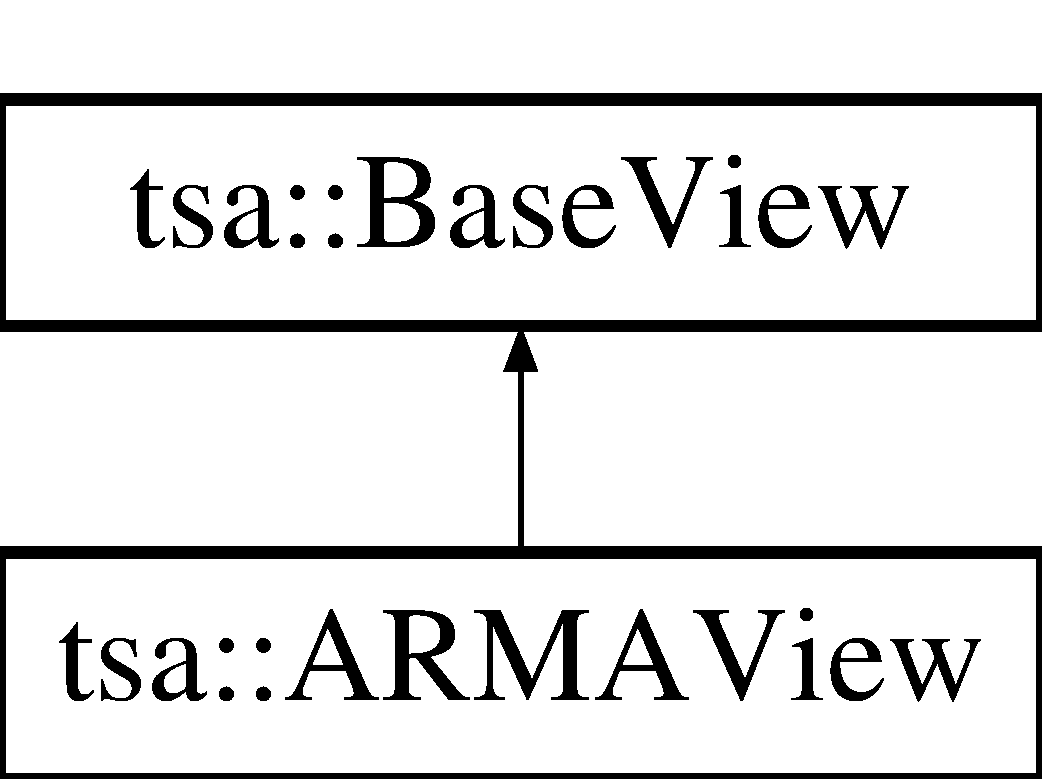
\includegraphics[height=2.000000cm]{classtsa_1_1_a_r_m_a_view}
\end{center}
\end{figure}
\subsection*{Public Member Functions}
\begin{DoxyCompactItemize}
\item 
\hyperlink{classtsa_1_1_a_r_m_a_view_a6b11811890252e645626e61fe434ea56}{A\+R\+M\+A\+View} (unsigned int maxP, unsigned int maxQ, int channels=1)
\item 
\hyperlink{classtsa_1_1_a_r_m_a_view_a1f28a41958cdf03016ffbae033a222bb}{A\+R\+M\+A\+View} (const \hyperlink{classtsa_1_1_a_r_m_a_view}{A\+R\+M\+A\+View} \&from)
\item 
\hyperlink{classtsa_1_1_a_r_m_a_view_a44779ce53323f8e6a1457974e9242004}{$\sim$\+A\+R\+M\+A\+View} ()
\item 
void \hyperlink{classtsa_1_1_a_r_m_a_view_aa6144eb86771f2c9d2cc95ac415acaba}{Load} (const char $\ast$filename, const char $\ast$fmt=\char`\"{}txt\char`\"{})
\item 
void \hyperlink{classtsa_1_1_a_r_m_a_view_a022ef32e6b0c2012707317cf1fbf9a54}{Save} (const char $\ast$filename, const char $\ast$fmt=\char`\"{}txt\char`\"{})
\item 
void \hyperlink{classtsa_1_1_a_r_m_a_view_ac667fd050280837056f3397fdb21afe6}{xml\+\_\+serialize} (\hyperlink{classeternity_1_1xml__archive}{eternity\+::xml\+\_\+archive} \&xml, const char $\ast$prefix)
\end{DoxyCompactItemize}
\begin{Indent}\textbf{ Getters}\par
\begin{DoxyCompactItemize}
\item 
const double \& \hyperlink{classtsa_1_1_a_r_m_a_view_a1a6f6606b2c5c8d0ef7d1484538e57d3}{Get\+AR} (int i, unsigned int channel=0) const
\item 
const double \& \hyperlink{classtsa_1_1_a_r_m_a_view_ad1f9e11168b5fb4c62ce4afb81ed0c86}{Get\+MA} (int i, unsigned int channel=0) const
\item 
const double \& \hyperlink{classtsa_1_1_a_r_m_a_view_a217094c2da79081413b74c8793dfbee3}{Get\+V\+AR} (int i, unsigned int channel1, unsigned int channel2) const
\item 
const double \& \hyperlink{classtsa_1_1_a_r_m_a_view_a60f3835003f645ba1947e34e08e58a27}{Get\+V\+MA} (int i, unsigned int channel1, unsigned int channel2) const
\item 
unsigned int \hyperlink{classtsa_1_1_a_r_m_a_view_a022eacefccd6be3b5efa36b656295206}{Get\+Ar\+Order} () const
\item 
unsigned int \hyperlink{classtsa_1_1_a_r_m_a_view_a50b9c68a7cafc52b47a35b11301d3adb}{Get\+Ma\+Order} () const
\item 
unsigned int \hyperlink{classtsa_1_1_a_r_m_a_view_a9a45f52a936aa86414c5afb43592f98e}{Get\+Channels} () const
\end{DoxyCompactItemize}
\end{Indent}
\begin{Indent}\textbf{ Setters}\par
\begin{DoxyCompactItemize}
\item 
void \hyperlink{classtsa_1_1_a_r_m_a_view_ae1b0323b27d5c8ad4a9e43a0119c407a}{Set\+AR} (int i, double v, unsigned int channel=0)
\item 
void \hyperlink{classtsa_1_1_a_r_m_a_view_a0fb548001ea80ac198ecf5619090320e}{Set\+MA} (int i, double v, unsigned int channel=0)
\item 
void \hyperlink{classtsa_1_1_a_r_m_a_view_a75a22d6966763cdba5788303a3fe3e7a}{Set\+V\+AR} (int i, double v, unsigned int channel1, unsigned int channel2)
\item 
void \hyperlink{classtsa_1_1_a_r_m_a_view_a3cebaae08e5718c57fb234c414904bc6}{Set\+V\+MA} (int i, double v, unsigned int channel1, unsigned int channel2)
\item 
void \hyperlink{classtsa_1_1_a_r_m_a_view_a192fe1e105780bc26cae74f51bc54597}{Set\+Order} (unsigned int maxP, unsigned int maxQ)
\item 
void \hyperlink{classtsa_1_1_a_r_m_a_view_a14f528f407a13473a7c20a0d7dec6482}{Set\+Channels} (unsigned int channels)
\end{DoxyCompactItemize}
\end{Indent}
\subsection*{Private Member Functions}
\begin{DoxyCompactItemize}
\item 
void \hyperlink{classtsa_1_1_a_r_m_a_view_a9fdd9c921d39b10a4d83379f69bdb160}{Resize\+AR} (unsigned int order)
\item 
void \hyperlink{classtsa_1_1_a_r_m_a_view_a757cddd07c0bb5bf0c4a8784e79f5900}{Resize\+MA} (unsigned int order)
\end{DoxyCompactItemize}
\subsection*{Private Attributes}
\begin{DoxyCompactItemize}
\item 
\hyperlink{namespacetsa_a6dd7105c3202ef00a213d7c029f5b248}{V\+Dmatrix} \hyperlink{classtsa_1_1_a_r_m_a_view_a0e95f26e07907a39ddb0e67b26fbc3ea}{m\+AR}
\begin{DoxyCompactList}\small\item\em The AR part of the process. \end{DoxyCompactList}\item 
\hyperlink{namespacetsa_a6dd7105c3202ef00a213d7c029f5b248}{V\+Dmatrix} \hyperlink{classtsa_1_1_a_r_m_a_view_a420b5083584d78e4bb7f5db8b3e62bc3}{m\+MA}
\begin{DoxyCompactList}\small\item\em The MA part of the process. \end{DoxyCompactList}\item 
unsigned int \hyperlink{classtsa_1_1_a_r_m_a_view_a0101f02d2c9f5eb2a6e6f1e1191fdb40}{m\+Channels}
\begin{DoxyCompactList}\small\item\em The dimension of the V\+A\+R\+MA process. \end{DoxyCompactList}\end{DoxyCompactItemize}
\subsection*{Additional Inherited Members}


\subsection{Detailed Description}
A\+R\+MA view\+: container for (vectorial) A\+R\+MA processes. 

A view for A\+R\+MA parametrization. It defines a general (V)A\+R\+MA process, which can be written as \[ \sum_{k=0}^{p} A^{(k)} \vec{y}_{n-k} = \sum_{k=0}^{q} B^{(k)} \vec{x}_{n-k} \] where A,B are square matrix of dimension d equal to the dimension of the input and output vectors x,y. If the order of the part MA q is equal to zero the process is an AR process. If the order of the AR part p is equal to zero the process is an MA process. Note that the matrix $A^{(0)}$ is assumed to be the identity. 

Definition at line 83 of file A\+R\+M\+A\+View.\+hpp.



\subsection{Constructor \& Destructor Documentation}
\mbox{\Hypertarget{classtsa_1_1_a_r_m_a_view_a6b11811890252e645626e61fe434ea56}\label{classtsa_1_1_a_r_m_a_view_a6b11811890252e645626e61fe434ea56}} 
\index{tsa\+::\+A\+R\+M\+A\+View@{tsa\+::\+A\+R\+M\+A\+View}!A\+R\+M\+A\+View@{A\+R\+M\+A\+View}}
\index{A\+R\+M\+A\+View@{A\+R\+M\+A\+View}!tsa\+::\+A\+R\+M\+A\+View@{tsa\+::\+A\+R\+M\+A\+View}}
\subsubsection{\texorpdfstring{A\+R\+M\+A\+View()}{ARMAView()}\hspace{0.1cm}{\footnotesize\ttfamily [1/2]}}
{\footnotesize\ttfamily tsa\+::\+A\+R\+M\+A\+View\+::\+A\+R\+M\+A\+View (\begin{DoxyParamCaption}\item[{unsigned int}]{maxP,  }\item[{unsigned int}]{maxQ,  }\item[{int}]{channels = {\ttfamily 1} }\end{DoxyParamCaption})\hspace{0.3cm}{\ttfamily [inline]}}

Constructor 
\begin{DoxyParams}{Parameters}
{\em maxP} & the order of the AR part \\
\hline
{\em maxQ} & the order of the MA part \\
\hline
{\em channels} & the dimension of \\
\hline
\end{DoxyParams}


Definition at line 92 of file A\+R\+M\+A\+View.\+hpp.

\mbox{\Hypertarget{classtsa_1_1_a_r_m_a_view_a1f28a41958cdf03016ffbae033a222bb}\label{classtsa_1_1_a_r_m_a_view_a1f28a41958cdf03016ffbae033a222bb}} 
\index{tsa\+::\+A\+R\+M\+A\+View@{tsa\+::\+A\+R\+M\+A\+View}!A\+R\+M\+A\+View@{A\+R\+M\+A\+View}}
\index{A\+R\+M\+A\+View@{A\+R\+M\+A\+View}!tsa\+::\+A\+R\+M\+A\+View@{tsa\+::\+A\+R\+M\+A\+View}}
\subsubsection{\texorpdfstring{A\+R\+M\+A\+View()}{ARMAView()}\hspace{0.1cm}{\footnotesize\ttfamily [2/2]}}
{\footnotesize\ttfamily tsa\+::\+A\+R\+M\+A\+View\+::\+A\+R\+M\+A\+View (\begin{DoxyParamCaption}\item[{const \hyperlink{classtsa_1_1_a_r_m_a_view}{A\+R\+M\+A\+View} \&}]{from }\end{DoxyParamCaption})\hspace{0.3cm}{\ttfamily [inline]}}

Copy constructor


\begin{DoxyParams}{Parameters}
{\em from} & The instance that must be copied \\
\hline
\end{DoxyParams}


Definition at line 106 of file A\+R\+M\+A\+View.\+hpp.

\mbox{\Hypertarget{classtsa_1_1_a_r_m_a_view_a44779ce53323f8e6a1457974e9242004}\label{classtsa_1_1_a_r_m_a_view_a44779ce53323f8e6a1457974e9242004}} 
\index{tsa\+::\+A\+R\+M\+A\+View@{tsa\+::\+A\+R\+M\+A\+View}!````~A\+R\+M\+A\+View@{$\sim$\+A\+R\+M\+A\+View}}
\index{````~A\+R\+M\+A\+View@{$\sim$\+A\+R\+M\+A\+View}!tsa\+::\+A\+R\+M\+A\+View@{tsa\+::\+A\+R\+M\+A\+View}}
\subsubsection{\texorpdfstring{$\sim$\+A\+R\+M\+A\+View()}{~ARMAView()}}
{\footnotesize\ttfamily tsa\+::\+A\+R\+M\+A\+View\+::$\sim$\+A\+R\+M\+A\+View (\begin{DoxyParamCaption}{ }\end{DoxyParamCaption})\hspace{0.3cm}{\ttfamily [inline]}}

Destructor 

Definition at line 119 of file A\+R\+M\+A\+View.\+hpp.



\subsection{Member Function Documentation}
\mbox{\Hypertarget{classtsa_1_1_a_r_m_a_view_a1a6f6606b2c5c8d0ef7d1484538e57d3}\label{classtsa_1_1_a_r_m_a_view_a1a6f6606b2c5c8d0ef7d1484538e57d3}} 
\index{tsa\+::\+A\+R\+M\+A\+View@{tsa\+::\+A\+R\+M\+A\+View}!Get\+AR@{Get\+AR}}
\index{Get\+AR@{Get\+AR}!tsa\+::\+A\+R\+M\+A\+View@{tsa\+::\+A\+R\+M\+A\+View}}
\subsubsection{\texorpdfstring{Get\+A\+R()}{GetAR()}}
{\footnotesize\ttfamily const double\& tsa\+::\+A\+R\+M\+A\+View\+::\+Get\+AR (\begin{DoxyParamCaption}\item[{int}]{i,  }\item[{unsigned int}]{channel = {\ttfamily 0} }\end{DoxyParamCaption}) const\hspace{0.3cm}{\ttfamily [inline]}}

This method gives the value of the AR\mbox{[}i\mbox{]} coefficient for one of the channels. It is assumed that the V\+A\+R\+MA process is diagonal, which means that there is and independent A\+R\+MA process for each channel.


\begin{DoxyParams}{Parameters}
{\em i} & the index of the AR coefficient \\
\hline
{\em channel} & the channel\\
\hline
\end{DoxyParams}
\begin{DoxyReturn}{Returns}
the value of the AR\mbox{[}i\mbox{]} coefficient 
\end{DoxyReturn}


Definition at line 241 of file A\+R\+M\+A\+View.\+hpp.

\mbox{\Hypertarget{classtsa_1_1_a_r_m_a_view_a022eacefccd6be3b5efa36b656295206}\label{classtsa_1_1_a_r_m_a_view_a022eacefccd6be3b5efa36b656295206}} 
\index{tsa\+::\+A\+R\+M\+A\+View@{tsa\+::\+A\+R\+M\+A\+View}!Get\+Ar\+Order@{Get\+Ar\+Order}}
\index{Get\+Ar\+Order@{Get\+Ar\+Order}!tsa\+::\+A\+R\+M\+A\+View@{tsa\+::\+A\+R\+M\+A\+View}}
\subsubsection{\texorpdfstring{Get\+Ar\+Order()}{GetArOrder()}}
{\footnotesize\ttfamily unsigned int tsa\+::\+A\+R\+M\+A\+View\+::\+Get\+Ar\+Order (\begin{DoxyParamCaption}{ }\end{DoxyParamCaption}) const\hspace{0.3cm}{\ttfamily [inline]}}

Get the order of the AR part of the process.

\begin{DoxyReturn}{Returns}
the order of the AR part of the process 
\end{DoxyReturn}


Definition at line 293 of file A\+R\+M\+A\+View.\+hpp.

\mbox{\Hypertarget{classtsa_1_1_a_r_m_a_view_a9a45f52a936aa86414c5afb43592f98e}\label{classtsa_1_1_a_r_m_a_view_a9a45f52a936aa86414c5afb43592f98e}} 
\index{tsa\+::\+A\+R\+M\+A\+View@{tsa\+::\+A\+R\+M\+A\+View}!Get\+Channels@{Get\+Channels}}
\index{Get\+Channels@{Get\+Channels}!tsa\+::\+A\+R\+M\+A\+View@{tsa\+::\+A\+R\+M\+A\+View}}
\subsubsection{\texorpdfstring{Get\+Channels()}{GetChannels()}}
{\footnotesize\ttfamily unsigned int tsa\+::\+A\+R\+M\+A\+View\+::\+Get\+Channels (\begin{DoxyParamCaption}{ }\end{DoxyParamCaption}) const\hspace{0.3cm}{\ttfamily [inline]}}

Get the dimension of the V\+A\+R\+MA process.

\begin{DoxyReturn}{Returns}
the dimension of the V\+A\+R\+MA process 
\end{DoxyReturn}


Definition at line 313 of file A\+R\+M\+A\+View.\+hpp.

\mbox{\Hypertarget{classtsa_1_1_a_r_m_a_view_ad1f9e11168b5fb4c62ce4afb81ed0c86}\label{classtsa_1_1_a_r_m_a_view_ad1f9e11168b5fb4c62ce4afb81ed0c86}} 
\index{tsa\+::\+A\+R\+M\+A\+View@{tsa\+::\+A\+R\+M\+A\+View}!Get\+MA@{Get\+MA}}
\index{Get\+MA@{Get\+MA}!tsa\+::\+A\+R\+M\+A\+View@{tsa\+::\+A\+R\+M\+A\+View}}
\subsubsection{\texorpdfstring{Get\+M\+A()}{GetMA()}}
{\footnotesize\ttfamily const double\& tsa\+::\+A\+R\+M\+A\+View\+::\+Get\+MA (\begin{DoxyParamCaption}\item[{int}]{i,  }\item[{unsigned int}]{channel = {\ttfamily 0} }\end{DoxyParamCaption}) const\hspace{0.3cm}{\ttfamily [inline]}}

This method gives the value of the MA\mbox{[}i\mbox{]} coefficient for one of the channels. It is assumed that the V\+A\+R\+MA process is diagonal, which means that there is and independent A\+R\+MA process for each channel.


\begin{DoxyParams}{Parameters}
{\em i} & the index of the MA coefficient \\
\hline
{\em channel} & the channel\\
\hline
\end{DoxyParams}
\begin{DoxyReturn}{Returns}
the value of the MA\mbox{[}i\mbox{]} coefficient 
\end{DoxyReturn}


Definition at line 256 of file A\+R\+M\+A\+View.\+hpp.

\mbox{\Hypertarget{classtsa_1_1_a_r_m_a_view_a50b9c68a7cafc52b47a35b11301d3adb}\label{classtsa_1_1_a_r_m_a_view_a50b9c68a7cafc52b47a35b11301d3adb}} 
\index{tsa\+::\+A\+R\+M\+A\+View@{tsa\+::\+A\+R\+M\+A\+View}!Get\+Ma\+Order@{Get\+Ma\+Order}}
\index{Get\+Ma\+Order@{Get\+Ma\+Order}!tsa\+::\+A\+R\+M\+A\+View@{tsa\+::\+A\+R\+M\+A\+View}}
\subsubsection{\texorpdfstring{Get\+Ma\+Order()}{GetMaOrder()}}
{\footnotesize\ttfamily unsigned int tsa\+::\+A\+R\+M\+A\+View\+::\+Get\+Ma\+Order (\begin{DoxyParamCaption}{ }\end{DoxyParamCaption}) const\hspace{0.3cm}{\ttfamily [inline]}}

Get the order of the MA part of the process.

\begin{DoxyReturn}{Returns}
the order of the MA part of the process 
\end{DoxyReturn}


Definition at line 303 of file A\+R\+M\+A\+View.\+hpp.

\mbox{\Hypertarget{classtsa_1_1_a_r_m_a_view_a217094c2da79081413b74c8793dfbee3}\label{classtsa_1_1_a_r_m_a_view_a217094c2da79081413b74c8793dfbee3}} 
\index{tsa\+::\+A\+R\+M\+A\+View@{tsa\+::\+A\+R\+M\+A\+View}!Get\+V\+AR@{Get\+V\+AR}}
\index{Get\+V\+AR@{Get\+V\+AR}!tsa\+::\+A\+R\+M\+A\+View@{tsa\+::\+A\+R\+M\+A\+View}}
\subsubsection{\texorpdfstring{Get\+V\+A\+R()}{GetVAR()}}
{\footnotesize\ttfamily const double\& tsa\+::\+A\+R\+M\+A\+View\+::\+Get\+V\+AR (\begin{DoxyParamCaption}\item[{int}]{i,  }\item[{unsigned int}]{channel1,  }\item[{unsigned int}]{channel2 }\end{DoxyParamCaption}) const\hspace{0.3cm}{\ttfamily [inline]}}

This method gives the value of the $A^{(i)}_{jk}$ coefficient for the V\+A\+R\+MA process


\begin{DoxyParams}{Parameters}
{\em i} & the index of the V\+AR coefficient \\
\hline
{\em channel1} & the first channel (index j) \\
\hline
{\em channel2} & the se channel (index k)\\
\hline
\end{DoxyParams}
\begin{DoxyReturn}{Returns}
the value of the coefficient $A^{(i)}_{jk}$ 
\end{DoxyReturn}


Definition at line 269 of file A\+R\+M\+A\+View.\+hpp.

\mbox{\Hypertarget{classtsa_1_1_a_r_m_a_view_a60f3835003f645ba1947e34e08e58a27}\label{classtsa_1_1_a_r_m_a_view_a60f3835003f645ba1947e34e08e58a27}} 
\index{tsa\+::\+A\+R\+M\+A\+View@{tsa\+::\+A\+R\+M\+A\+View}!Get\+V\+MA@{Get\+V\+MA}}
\index{Get\+V\+MA@{Get\+V\+MA}!tsa\+::\+A\+R\+M\+A\+View@{tsa\+::\+A\+R\+M\+A\+View}}
\subsubsection{\texorpdfstring{Get\+V\+M\+A()}{GetVMA()}}
{\footnotesize\ttfamily const double\& tsa\+::\+A\+R\+M\+A\+View\+::\+Get\+V\+MA (\begin{DoxyParamCaption}\item[{int}]{i,  }\item[{unsigned int}]{channel1,  }\item[{unsigned int}]{channel2 }\end{DoxyParamCaption}) const\hspace{0.3cm}{\ttfamily [inline]}}

This method gives the value of the $B^{(i)}_{jk}$ coefficient for the V\+A\+R\+MA process


\begin{DoxyParams}{Parameters}
{\em i} & the index of the V\+MA coefficient \\
\hline
{\em channel1} & the first channel (index j) \\
\hline
{\em channel2} & the se channel (index k)\\
\hline
\end{DoxyParams}
\begin{DoxyReturn}{Returns}
the value of the coefficient $B^{(i)}_{jk}$ 
\end{DoxyReturn}


Definition at line 282 of file A\+R\+M\+A\+View.\+hpp.

\mbox{\Hypertarget{classtsa_1_1_a_r_m_a_view_aa6144eb86771f2c9d2cc95ac415acaba}\label{classtsa_1_1_a_r_m_a_view_aa6144eb86771f2c9d2cc95ac415acaba}} 
\index{tsa\+::\+A\+R\+M\+A\+View@{tsa\+::\+A\+R\+M\+A\+View}!Load@{Load}}
\index{Load@{Load}!tsa\+::\+A\+R\+M\+A\+View@{tsa\+::\+A\+R\+M\+A\+View}}
\subsubsection{\texorpdfstring{Load()}{Load()}}
{\footnotesize\ttfamily void tsa\+::\+A\+R\+M\+A\+View\+::\+Load (\begin{DoxyParamCaption}\item[{const char $\ast$}]{filename,  }\item[{const char $\ast$}]{fmt = {\ttfamily \char`\"{}txt\char`\"{}} }\end{DoxyParamCaption})\hspace{0.3cm}{\ttfamily [inline]}}



Definition at line 122 of file A\+R\+M\+A\+View.\+hpp.

\mbox{\Hypertarget{classtsa_1_1_a_r_m_a_view_a9fdd9c921d39b10a4d83379f69bdb160}\label{classtsa_1_1_a_r_m_a_view_a9fdd9c921d39b10a4d83379f69bdb160}} 
\index{tsa\+::\+A\+R\+M\+A\+View@{tsa\+::\+A\+R\+M\+A\+View}!Resize\+AR@{Resize\+AR}}
\index{Resize\+AR@{Resize\+AR}!tsa\+::\+A\+R\+M\+A\+View@{tsa\+::\+A\+R\+M\+A\+View}}
\subsubsection{\texorpdfstring{Resize\+A\+R()}{ResizeAR()}}
{\footnotesize\ttfamily void tsa\+::\+A\+R\+M\+A\+View\+::\+Resize\+AR (\begin{DoxyParamCaption}\item[{unsigned int}]{order }\end{DoxyParamCaption})\hspace{0.3cm}{\ttfamily [inline]}, {\ttfamily [private]}}

This method change the order of the AR part of the process


\begin{DoxyParams}{Parameters}
{\em order} & the new order of the AR part \\
\hline
\end{DoxyParams}


Definition at line 420 of file A\+R\+M\+A\+View.\+hpp.

\mbox{\Hypertarget{classtsa_1_1_a_r_m_a_view_a757cddd07c0bb5bf0c4a8784e79f5900}\label{classtsa_1_1_a_r_m_a_view_a757cddd07c0bb5bf0c4a8784e79f5900}} 
\index{tsa\+::\+A\+R\+M\+A\+View@{tsa\+::\+A\+R\+M\+A\+View}!Resize\+MA@{Resize\+MA}}
\index{Resize\+MA@{Resize\+MA}!tsa\+::\+A\+R\+M\+A\+View@{tsa\+::\+A\+R\+M\+A\+View}}
\subsubsection{\texorpdfstring{Resize\+M\+A()}{ResizeMA()}}
{\footnotesize\ttfamily void tsa\+::\+A\+R\+M\+A\+View\+::\+Resize\+MA (\begin{DoxyParamCaption}\item[{unsigned int}]{order }\end{DoxyParamCaption})\hspace{0.3cm}{\ttfamily [inline]}, {\ttfamily [private]}}

This method change the order of the MA part of the process


\begin{DoxyParams}{Parameters}
{\em order} & the new order of the MA part \\
\hline
\end{DoxyParams}


Definition at line 437 of file A\+R\+M\+A\+View.\+hpp.

\mbox{\Hypertarget{classtsa_1_1_a_r_m_a_view_a022ef32e6b0c2012707317cf1fbf9a54}\label{classtsa_1_1_a_r_m_a_view_a022ef32e6b0c2012707317cf1fbf9a54}} 
\index{tsa\+::\+A\+R\+M\+A\+View@{tsa\+::\+A\+R\+M\+A\+View}!Save@{Save}}
\index{Save@{Save}!tsa\+::\+A\+R\+M\+A\+View@{tsa\+::\+A\+R\+M\+A\+View}}
\subsubsection{\texorpdfstring{Save()}{Save()}}
{\footnotesize\ttfamily void tsa\+::\+A\+R\+M\+A\+View\+::\+Save (\begin{DoxyParamCaption}\item[{const char $\ast$}]{filename,  }\item[{const char $\ast$}]{fmt = {\ttfamily \char`\"{}txt\char`\"{}} }\end{DoxyParamCaption})\hspace{0.3cm}{\ttfamily [inline]}}



Definition at line 129 of file A\+R\+M\+A\+View.\+hpp.

\mbox{\Hypertarget{classtsa_1_1_a_r_m_a_view_ae1b0323b27d5c8ad4a9e43a0119c407a}\label{classtsa_1_1_a_r_m_a_view_ae1b0323b27d5c8ad4a9e43a0119c407a}} 
\index{tsa\+::\+A\+R\+M\+A\+View@{tsa\+::\+A\+R\+M\+A\+View}!Set\+AR@{Set\+AR}}
\index{Set\+AR@{Set\+AR}!tsa\+::\+A\+R\+M\+A\+View@{tsa\+::\+A\+R\+M\+A\+View}}
\subsubsection{\texorpdfstring{Set\+A\+R()}{SetAR()}}
{\footnotesize\ttfamily void tsa\+::\+A\+R\+M\+A\+View\+::\+Set\+AR (\begin{DoxyParamCaption}\item[{int}]{i,  }\item[{double}]{v,  }\item[{unsigned int}]{channel = {\ttfamily 0} }\end{DoxyParamCaption})\hspace{0.3cm}{\ttfamily [inline]}}

This method sets the value of the AR\mbox{[}i\mbox{]} coefficient for one of the channels. It is assumed that the V\+A\+R\+MA process is diagonal, which means that there is and independent A\+R\+MA process for each channel.


\begin{DoxyParams}{Parameters}
{\em i} & the index of the AR part \\
\hline
{\em v} & the new value of AR\mbox{[}i\mbox{]} \\
\hline
{\em channel} & the channel \\
\hline
\end{DoxyParams}


Definition at line 334 of file A\+R\+M\+A\+View.\+hpp.

\mbox{\Hypertarget{classtsa_1_1_a_r_m_a_view_a14f528f407a13473a7c20a0d7dec6482}\label{classtsa_1_1_a_r_m_a_view_a14f528f407a13473a7c20a0d7dec6482}} 
\index{tsa\+::\+A\+R\+M\+A\+View@{tsa\+::\+A\+R\+M\+A\+View}!Set\+Channels@{Set\+Channels}}
\index{Set\+Channels@{Set\+Channels}!tsa\+::\+A\+R\+M\+A\+View@{tsa\+::\+A\+R\+M\+A\+View}}
\subsubsection{\texorpdfstring{Set\+Channels()}{SetChannels()}}
{\footnotesize\ttfamily void tsa\+::\+A\+R\+M\+A\+View\+::\+Set\+Channels (\begin{DoxyParamCaption}\item[{unsigned int}]{channels }\end{DoxyParamCaption})\hspace{0.3cm}{\ttfamily [inline]}}

This method sets the dimension of the V\+A\+R\+MA process


\begin{DoxyParams}{Parameters}
{\em channels} & the dimension of the V\+A\+R\+MA process \\
\hline
\end{DoxyParams}


Definition at line 399 of file A\+R\+M\+A\+View.\+hpp.

\mbox{\Hypertarget{classtsa_1_1_a_r_m_a_view_a0fb548001ea80ac198ecf5619090320e}\label{classtsa_1_1_a_r_m_a_view_a0fb548001ea80ac198ecf5619090320e}} 
\index{tsa\+::\+A\+R\+M\+A\+View@{tsa\+::\+A\+R\+M\+A\+View}!Set\+MA@{Set\+MA}}
\index{Set\+MA@{Set\+MA}!tsa\+::\+A\+R\+M\+A\+View@{tsa\+::\+A\+R\+M\+A\+View}}
\subsubsection{\texorpdfstring{Set\+M\+A()}{SetMA()}}
{\footnotesize\ttfamily void tsa\+::\+A\+R\+M\+A\+View\+::\+Set\+MA (\begin{DoxyParamCaption}\item[{int}]{i,  }\item[{double}]{v,  }\item[{unsigned int}]{channel = {\ttfamily 0} }\end{DoxyParamCaption})\hspace{0.3cm}{\ttfamily [inline]}}

This method sets the value of the MA\mbox{[}i\mbox{]} coefficient for one of the channels. It is assumed that the V\+A\+R\+MA process is diagonal, which means that there is and independent A\+R\+MA process for each channel.


\begin{DoxyParams}{Parameters}
{\em i} & the index of the MA part \\
\hline
{\em v} & the new value of MA\mbox{[}i\mbox{]} \\
\hline
{\em channel} & the channel \\
\hline
\end{DoxyParams}


Definition at line 347 of file A\+R\+M\+A\+View.\+hpp.

\mbox{\Hypertarget{classtsa_1_1_a_r_m_a_view_a192fe1e105780bc26cae74f51bc54597}\label{classtsa_1_1_a_r_m_a_view_a192fe1e105780bc26cae74f51bc54597}} 
\index{tsa\+::\+A\+R\+M\+A\+View@{tsa\+::\+A\+R\+M\+A\+View}!Set\+Order@{Set\+Order}}
\index{Set\+Order@{Set\+Order}!tsa\+::\+A\+R\+M\+A\+View@{tsa\+::\+A\+R\+M\+A\+View}}
\subsubsection{\texorpdfstring{Set\+Order()}{SetOrder()}}
{\footnotesize\ttfamily void tsa\+::\+A\+R\+M\+A\+View\+::\+Set\+Order (\begin{DoxyParamCaption}\item[{unsigned int}]{maxP,  }\item[{unsigned int}]{maxQ }\end{DoxyParamCaption})\hspace{0.3cm}{\ttfamily [inline]}}

This methods sets the order (p,q) of the (V)A\+R\+MA process


\begin{DoxyParams}{Parameters}
{\em maxP} & the order of the AR part of the process \\
\hline
{\em maxQ} & the order of the MA part of the process \\
\hline
\end{DoxyParams}


Definition at line 386 of file A\+R\+M\+A\+View.\+hpp.

\mbox{\Hypertarget{classtsa_1_1_a_r_m_a_view_a75a22d6966763cdba5788303a3fe3e7a}\label{classtsa_1_1_a_r_m_a_view_a75a22d6966763cdba5788303a3fe3e7a}} 
\index{tsa\+::\+A\+R\+M\+A\+View@{tsa\+::\+A\+R\+M\+A\+View}!Set\+V\+AR@{Set\+V\+AR}}
\index{Set\+V\+AR@{Set\+V\+AR}!tsa\+::\+A\+R\+M\+A\+View@{tsa\+::\+A\+R\+M\+A\+View}}
\subsubsection{\texorpdfstring{Set\+V\+A\+R()}{SetVAR()}}
{\footnotesize\ttfamily void tsa\+::\+A\+R\+M\+A\+View\+::\+Set\+V\+AR (\begin{DoxyParamCaption}\item[{int}]{i,  }\item[{double}]{v,  }\item[{unsigned int}]{channel1,  }\item[{unsigned int}]{channel2 }\end{DoxyParamCaption})\hspace{0.3cm}{\ttfamily [inline]}}

This method sets the value of the $A^{(i)}_{jk}$ coefficient for the V\+A\+R\+MA process


\begin{DoxyParams}{Parameters}
{\em i} & the index of the V\+AR coefficient \\
\hline
{\em v} & the new value of $A^{(i)}_{jk}$ \\
\hline
{\em channel1} & the first channel (index j) \\
\hline
{\em channel2} & the se channel (index k) \\
\hline
\end{DoxyParams}


Definition at line 361 of file A\+R\+M\+A\+View.\+hpp.

\mbox{\Hypertarget{classtsa_1_1_a_r_m_a_view_a3cebaae08e5718c57fb234c414904bc6}\label{classtsa_1_1_a_r_m_a_view_a3cebaae08e5718c57fb234c414904bc6}} 
\index{tsa\+::\+A\+R\+M\+A\+View@{tsa\+::\+A\+R\+M\+A\+View}!Set\+V\+MA@{Set\+V\+MA}}
\index{Set\+V\+MA@{Set\+V\+MA}!tsa\+::\+A\+R\+M\+A\+View@{tsa\+::\+A\+R\+M\+A\+View}}
\subsubsection{\texorpdfstring{Set\+V\+M\+A()}{SetVMA()}}
{\footnotesize\ttfamily void tsa\+::\+A\+R\+M\+A\+View\+::\+Set\+V\+MA (\begin{DoxyParamCaption}\item[{int}]{i,  }\item[{double}]{v,  }\item[{unsigned int}]{channel1,  }\item[{unsigned int}]{channel2 }\end{DoxyParamCaption})\hspace{0.3cm}{\ttfamily [inline]}}

This method sets the value of the $B^{(i)}_{jk}$ coefficient for the V\+A\+R\+MA process


\begin{DoxyParams}{Parameters}
{\em i} & the index of the V\+AR coefficient \\
\hline
{\em v} & the new value of $B^{(i)}_{jk}$ \\
\hline
{\em channel1} & the first channel (index j) \\
\hline
{\em channel2} & the se channel (index k) \\
\hline
\end{DoxyParams}


Definition at line 375 of file A\+R\+M\+A\+View.\+hpp.

\mbox{\Hypertarget{classtsa_1_1_a_r_m_a_view_ac667fd050280837056f3397fdb21afe6}\label{classtsa_1_1_a_r_m_a_view_ac667fd050280837056f3397fdb21afe6}} 
\index{tsa\+::\+A\+R\+M\+A\+View@{tsa\+::\+A\+R\+M\+A\+View}!xml\+\_\+serialize@{xml\+\_\+serialize}}
\index{xml\+\_\+serialize@{xml\+\_\+serialize}!tsa\+::\+A\+R\+M\+A\+View@{tsa\+::\+A\+R\+M\+A\+View}}
\subsubsection{\texorpdfstring{xml\+\_\+serialize()}{xml\_serialize()}}
{\footnotesize\ttfamily void tsa\+::\+A\+R\+M\+A\+View\+::xml\+\_\+serialize (\begin{DoxyParamCaption}\item[{\hyperlink{classeternity_1_1xml__archive}{eternity\+::xml\+\_\+archive} \&}]{xml,  }\item[{const char $\ast$}]{prefix }\end{DoxyParamCaption})\hspace{0.3cm}{\ttfamily [inline]}}



Definition at line 136 of file A\+R\+M\+A\+View.\+hpp.



\subsection{Member Data Documentation}
\mbox{\Hypertarget{classtsa_1_1_a_r_m_a_view_a0e95f26e07907a39ddb0e67b26fbc3ea}\label{classtsa_1_1_a_r_m_a_view_a0e95f26e07907a39ddb0e67b26fbc3ea}} 
\index{tsa\+::\+A\+R\+M\+A\+View@{tsa\+::\+A\+R\+M\+A\+View}!m\+AR@{m\+AR}}
\index{m\+AR@{m\+AR}!tsa\+::\+A\+R\+M\+A\+View@{tsa\+::\+A\+R\+M\+A\+View}}
\subsubsection{\texorpdfstring{m\+AR}{mAR}}
{\footnotesize\ttfamily \hyperlink{namespacetsa_a6dd7105c3202ef00a213d7c029f5b248}{V\+Dmatrix} tsa\+::\+A\+R\+M\+A\+View\+::m\+AR\hspace{0.3cm}{\ttfamily [private]}}



The AR part of the process. 



Definition at line 446 of file A\+R\+M\+A\+View.\+hpp.

\mbox{\Hypertarget{classtsa_1_1_a_r_m_a_view_a0101f02d2c9f5eb2a6e6f1e1191fdb40}\label{classtsa_1_1_a_r_m_a_view_a0101f02d2c9f5eb2a6e6f1e1191fdb40}} 
\index{tsa\+::\+A\+R\+M\+A\+View@{tsa\+::\+A\+R\+M\+A\+View}!m\+Channels@{m\+Channels}}
\index{m\+Channels@{m\+Channels}!tsa\+::\+A\+R\+M\+A\+View@{tsa\+::\+A\+R\+M\+A\+View}}
\subsubsection{\texorpdfstring{m\+Channels}{mChannels}}
{\footnotesize\ttfamily unsigned int tsa\+::\+A\+R\+M\+A\+View\+::m\+Channels\hspace{0.3cm}{\ttfamily [private]}}



The dimension of the V\+A\+R\+MA process. 



Definition at line 450 of file A\+R\+M\+A\+View.\+hpp.

\mbox{\Hypertarget{classtsa_1_1_a_r_m_a_view_a420b5083584d78e4bb7f5db8b3e62bc3}\label{classtsa_1_1_a_r_m_a_view_a420b5083584d78e4bb7f5db8b3e62bc3}} 
\index{tsa\+::\+A\+R\+M\+A\+View@{tsa\+::\+A\+R\+M\+A\+View}!m\+MA@{m\+MA}}
\index{m\+MA@{m\+MA}!tsa\+::\+A\+R\+M\+A\+View@{tsa\+::\+A\+R\+M\+A\+View}}
\subsubsection{\texorpdfstring{m\+MA}{mMA}}
{\footnotesize\ttfamily \hyperlink{namespacetsa_a6dd7105c3202ef00a213d7c029f5b248}{V\+Dmatrix} tsa\+::\+A\+R\+M\+A\+View\+::m\+MA\hspace{0.3cm}{\ttfamily [private]}}



The MA part of the process. 



Definition at line 449 of file A\+R\+M\+A\+View.\+hpp.



The documentation for this class was generated from the following file\+:\begin{DoxyCompactItemize}
\item 
/home/filip/\+Ph\+D/\+W\+D\+F\+Pipe\+\_\+test/p4\+T\+S\+A/include/\hyperlink{_a_r_m_a_view_8hpp}{A\+R\+M\+A\+View.\+hpp}\end{DoxyCompactItemize}

\hypertarget{structeternity_1_1association}{}\section{eternity\+:\+:association$<$ First\+Content, Second\+Content $>$ Struct Template Reference}
\label{structeternity_1_1association}\index{eternity\+::association$<$ First\+Content, Second\+Content $>$@{eternity\+::association$<$ First\+Content, Second\+Content $>$}}


{\ttfamily \#include $<$algorithms.\+hpp$>$}

\subsection*{Public Member Functions}
\begin{DoxyCompactItemize}
\item 
{\footnotesize template$<$class Input\+Iterator , class Archive $>$ }\\size\+\_\+t \hyperlink{structeternity_1_1association_a826dce070ffd89015b66ea9ea26c07e2}{xml\+\_\+write} (Input\+Iterator first, Input\+Iterator last, Archive \&\hyperlink{classeternity_1_1archive}{archive})
\item 
{\footnotesize template$<$class Container , class Input\+Iterator , class Archive $>$ }\\void \hyperlink{structeternity_1_1association_a2f1c27b77cd84364c498feb134864d4f}{xml\+\_\+read} (Container \&container, Input\+Iterator insert, size\+\_\+t len, Archive \&\hyperlink{classeternity_1_1archive}{archive})
\item 
{\footnotesize template$<$class Input\+Iterator , class Archive $>$ }\\size\+\_\+t \hyperlink{structeternity_1_1association_a927d1de7c19bce31622b31417e107ebe}{write} (Input\+Iterator first, Input\+Iterator last, Archive \&\hyperlink{classeternity_1_1archive}{archive})
\item 
{\footnotesize template$<$class Container , class Input\+Iterator , class Archive $>$ }\\void \hyperlink{structeternity_1_1association_ab488701a51e5c139347c7c5acc88d05e}{read} (Container \&container, Input\+Iterator insert, size\+\_\+t len, Archive \&\hyperlink{classeternity_1_1archive}{archive})
\end{DoxyCompactItemize}


\subsection{Detailed Description}
\subsubsection*{template$<$class First\+Content, class Second\+Content$>$\newline
struct eternity\+::association$<$ First\+Content, Second\+Content $>$}

Manage persistence of associtative containers (e.\+g. map or set). Use template parameter to specify contents type of key (e.\+g. primitives, objects or pointers) and the content type of data (again one from primitives, objects or pointers). This struct is not intended to direct use but must be passed as template parameter of xml\+\_\+serialize() or serialize() algorithms. 

Definition at line 227 of file algorithms.\+hpp.



\subsection{Member Function Documentation}
\mbox{\Hypertarget{structeternity_1_1association_ab488701a51e5c139347c7c5acc88d05e}\label{structeternity_1_1association_ab488701a51e5c139347c7c5acc88d05e}} 
\index{eternity\+::association@{eternity\+::association}!read@{read}}
\index{read@{read}!eternity\+::association@{eternity\+::association}}
\subsubsection{\texorpdfstring{read()}{read()}}
{\footnotesize\ttfamily template$<$class First\+Content , class Second\+Content $>$ \\
template$<$class Container , class Input\+Iterator , class Archive $>$ \\
void \hyperlink{structeternity_1_1association}{eternity\+::association}$<$ First\+Content, Second\+Content $>$\+::read (\begin{DoxyParamCaption}\item[{Container \&}]{container,  }\item[{Input\+Iterator}]{insert,  }\item[{size\+\_\+t}]{len,  }\item[{Archive \&}]{archive }\end{DoxyParamCaption})}



Definition at line 289 of file algorithms.\+hpp.

\mbox{\Hypertarget{structeternity_1_1association_a927d1de7c19bce31622b31417e107ebe}\label{structeternity_1_1association_a927d1de7c19bce31622b31417e107ebe}} 
\index{eternity\+::association@{eternity\+::association}!write@{write}}
\index{write@{write}!eternity\+::association@{eternity\+::association}}
\subsubsection{\texorpdfstring{write()}{write()}}
{\footnotesize\ttfamily template$<$class First\+Content , class Second\+Content $>$ \\
template$<$class Input\+Iterator , class Archive $>$ \\
size\+\_\+t \hyperlink{structeternity_1_1association}{eternity\+::association}$<$ First\+Content, Second\+Content $>$\+::write (\begin{DoxyParamCaption}\item[{Input\+Iterator}]{first,  }\item[{Input\+Iterator}]{last,  }\item[{Archive \&}]{archive }\end{DoxyParamCaption})}



Definition at line 275 of file algorithms.\+hpp.

\mbox{\Hypertarget{structeternity_1_1association_a2f1c27b77cd84364c498feb134864d4f}\label{structeternity_1_1association_a2f1c27b77cd84364c498feb134864d4f}} 
\index{eternity\+::association@{eternity\+::association}!xml\+\_\+read@{xml\+\_\+read}}
\index{xml\+\_\+read@{xml\+\_\+read}!eternity\+::association@{eternity\+::association}}
\subsubsection{\texorpdfstring{xml\+\_\+read()}{xml\_read()}}
{\footnotesize\ttfamily template$<$class First\+Content , class Second\+Content $>$ \\
template$<$class Container , class Input\+Iterator , class Archive $>$ \\
void \hyperlink{structeternity_1_1association}{eternity\+::association}$<$ First\+Content, Second\+Content $>$\+::xml\+\_\+read (\begin{DoxyParamCaption}\item[{Container \&}]{container,  }\item[{Input\+Iterator}]{insert,  }\item[{size\+\_\+t}]{len,  }\item[{Archive \&}]{archive }\end{DoxyParamCaption})}



Definition at line 256 of file algorithms.\+hpp.

\mbox{\Hypertarget{structeternity_1_1association_a826dce070ffd89015b66ea9ea26c07e2}\label{structeternity_1_1association_a826dce070ffd89015b66ea9ea26c07e2}} 
\index{eternity\+::association@{eternity\+::association}!xml\+\_\+write@{xml\+\_\+write}}
\index{xml\+\_\+write@{xml\+\_\+write}!eternity\+::association@{eternity\+::association}}
\subsubsection{\texorpdfstring{xml\+\_\+write()}{xml\_write()}}
{\footnotesize\ttfamily template$<$class First\+Content , class Second\+Content $>$ \\
template$<$class Input\+Iterator , class Archive $>$ \\
size\+\_\+t \hyperlink{structeternity_1_1association}{eternity\+::association}$<$ First\+Content, Second\+Content $>$\+::xml\+\_\+write (\begin{DoxyParamCaption}\item[{Input\+Iterator}]{first,  }\item[{Input\+Iterator}]{last,  }\item[{Archive \&}]{archive }\end{DoxyParamCaption})}



Definition at line 242 of file algorithms.\+hpp.



The documentation for this struct was generated from the following file\+:\begin{DoxyCompactItemize}
\item 
/home/filip/\+Ph\+D/\+W\+D\+F\+Pipe\+\_\+test/p4\+T\+S\+A/include/eternity/\hyperlink{algorithms_8hpp}{algorithms.\+hpp}\end{DoxyCompactItemize}

\hypertarget{classtsa_1_1bad__matrix__size}{}\section{tsa\+:\+:bad\+\_\+matrix\+\_\+size Class Reference}
\label{classtsa_1_1bad__matrix__size}\index{tsa\+::bad\+\_\+matrix\+\_\+size@{tsa\+::bad\+\_\+matrix\+\_\+size}}


{\ttfamily \#include $<$Algo\+Exceptions.\+hpp$>$}

Inheritance diagram for tsa\+:\+:bad\+\_\+matrix\+\_\+size\+:\begin{figure}[H]
\begin{center}
\leavevmode
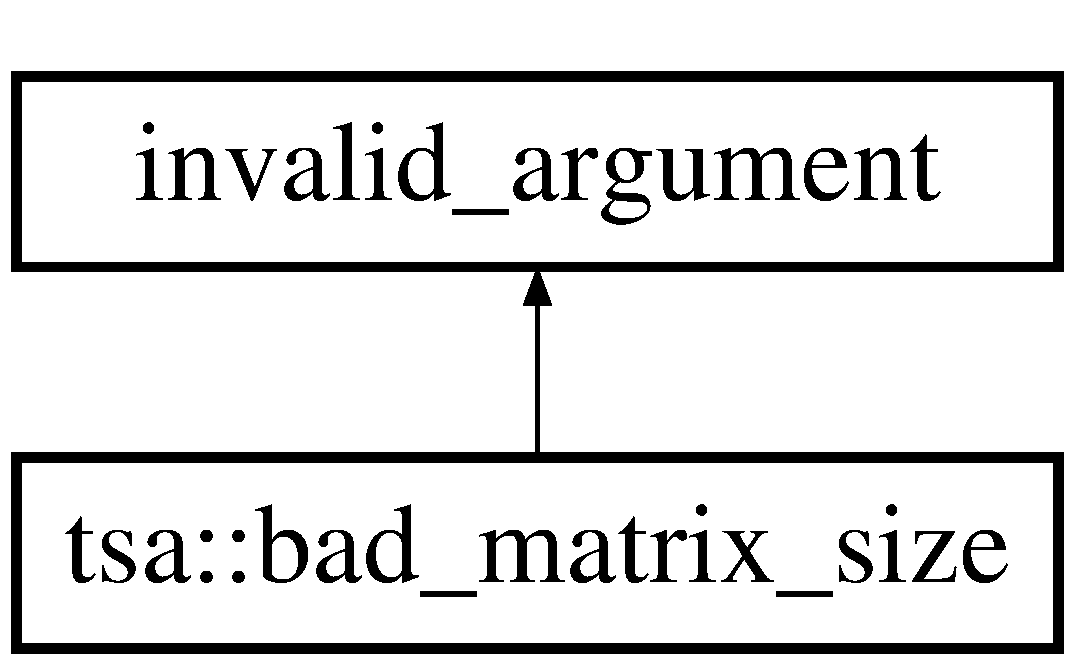
\includegraphics[height=2.000000cm]{classtsa_1_1bad__matrix__size}
\end{center}
\end{figure}
\subsection*{Public Member Functions}
\begin{DoxyCompactItemize}
\item 
\hyperlink{classtsa_1_1bad__matrix__size_a5d06e7b24038b0b1ff07a0fa308f8e54}{bad\+\_\+matrix\+\_\+size} (const std\+::string \&msg)
\end{DoxyCompactItemize}


\subsection{Detailed Description}
This exception should be used when a matrix argument of an algorithm has an incorrect size. It contains information about the correct expected size. 

Definition at line 72 of file Algo\+Exceptions.\+hpp.



\subsection{Constructor \& Destructor Documentation}
\mbox{\Hypertarget{classtsa_1_1bad__matrix__size_a5d06e7b24038b0b1ff07a0fa308f8e54}\label{classtsa_1_1bad__matrix__size_a5d06e7b24038b0b1ff07a0fa308f8e54}} 
\index{tsa\+::bad\+\_\+matrix\+\_\+size@{tsa\+::bad\+\_\+matrix\+\_\+size}!bad\+\_\+matrix\+\_\+size@{bad\+\_\+matrix\+\_\+size}}
\index{bad\+\_\+matrix\+\_\+size@{bad\+\_\+matrix\+\_\+size}!tsa\+::bad\+\_\+matrix\+\_\+size@{tsa\+::bad\+\_\+matrix\+\_\+size}}
\subsubsection{\texorpdfstring{bad\+\_\+matrix\+\_\+size()}{bad\_matrix\_size()}}
{\footnotesize\ttfamily tsa\+::bad\+\_\+matrix\+\_\+size\+::bad\+\_\+matrix\+\_\+size (\begin{DoxyParamCaption}\item[{const std\+::string \&}]{msg }\end{DoxyParamCaption})\hspace{0.3cm}{\ttfamily [inline]}}

Constructor


\begin{DoxyParams}{Parameters}
{\em msg} & error message \\
\hline
\end{DoxyParams}


Definition at line 80 of file Algo\+Exceptions.\+hpp.



The documentation for this class was generated from the following file\+:\begin{DoxyCompactItemize}
\item 
/home/filip/\+Ph\+D/\+W\+D\+F\+Pipe\+\_\+test/p4\+T\+S\+A/include/\hyperlink{_algo_exceptions_8hpp}{Algo\+Exceptions.\+hpp}\end{DoxyCompactItemize}

\hypertarget{classtsa_1_1bad__value}{}\section{tsa\+:\+:bad\+\_\+value Class Reference}
\label{classtsa_1_1bad__value}\index{tsa\+::bad\+\_\+value@{tsa\+::bad\+\_\+value}}


{\ttfamily \#include $<$Algo\+Exceptions.\+hpp$>$}

Inheritance diagram for tsa\+:\+:bad\+\_\+value\+:\begin{figure}[H]
\begin{center}
\leavevmode
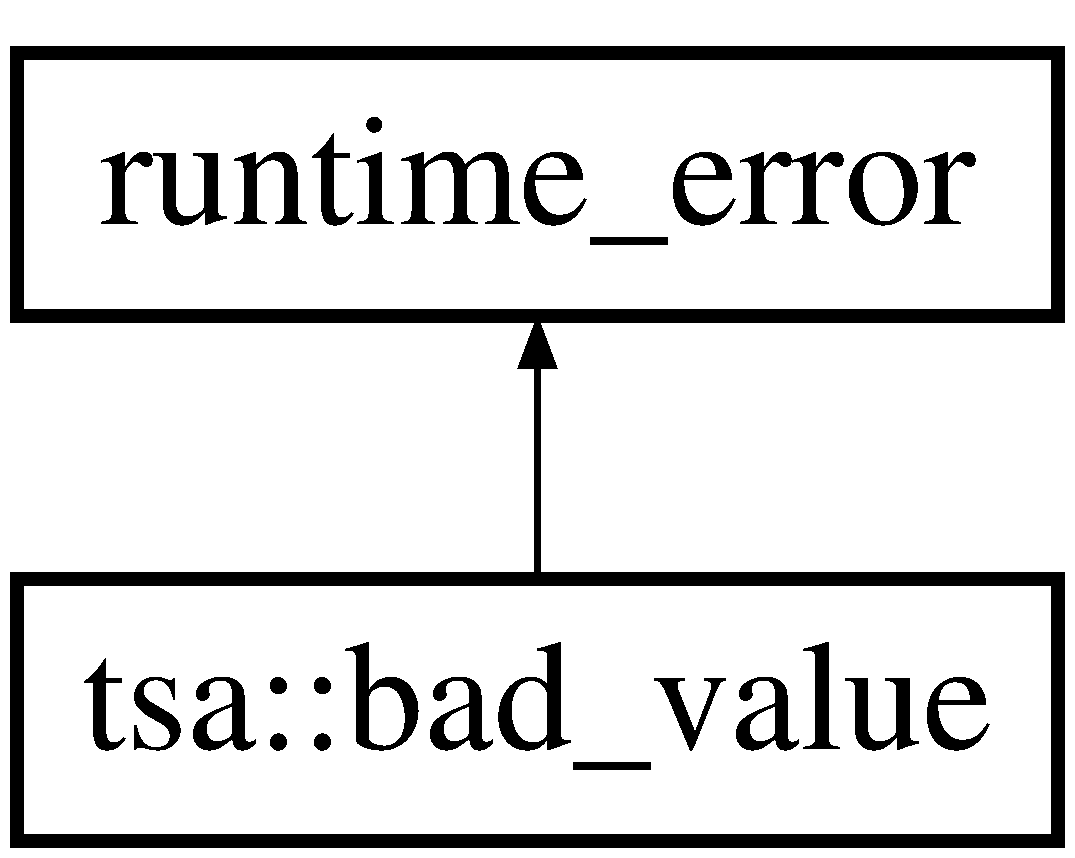
\includegraphics[height=2.000000cm]{classtsa_1_1bad__value}
\end{center}
\end{figure}
\subsection*{Public Member Functions}
\begin{DoxyCompactItemize}
\item 
\hyperlink{classtsa_1_1bad__value_a23b7068f35f29697bb817109e378bd8e}{bad\+\_\+value} ()
\end{DoxyCompactItemize}


\subsection{Detailed Description}
This exception should be used when some processed data cannot be returned 

Definition at line 145 of file Algo\+Exceptions.\+hpp.



\subsection{Constructor \& Destructor Documentation}
\mbox{\Hypertarget{classtsa_1_1bad__value_a23b7068f35f29697bb817109e378bd8e}\label{classtsa_1_1bad__value_a23b7068f35f29697bb817109e378bd8e}} 
\index{tsa\+::bad\+\_\+value@{tsa\+::bad\+\_\+value}!bad\+\_\+value@{bad\+\_\+value}}
\index{bad\+\_\+value@{bad\+\_\+value}!tsa\+::bad\+\_\+value@{tsa\+::bad\+\_\+value}}
\subsubsection{\texorpdfstring{bad\+\_\+value()}{bad\_value()}}
{\footnotesize\ttfamily tsa\+::bad\+\_\+value\+::bad\+\_\+value (\begin{DoxyParamCaption}{ }\end{DoxyParamCaption})\hspace{0.3cm}{\ttfamily [inline]}}

Constructor


\begin{DoxyParams}{Parameters}
{\em msg} & error message \\
\hline
\end{DoxyParams}


Definition at line 153 of file Algo\+Exceptions.\+hpp.



The documentation for this class was generated from the following file\+:\begin{DoxyCompactItemize}
\item 
/home/filip/\+Ph\+D/\+W\+D\+F\+Pipe\+\_\+test/p4\+T\+S\+A/include/\hyperlink{_algo_exceptions_8hpp}{Algo\+Exceptions.\+hpp}\end{DoxyCompactItemize}

\hypertarget{classtsa_1_1bad__vector__size}{}\section{tsa\+:\+:bad\+\_\+vector\+\_\+size Class Reference}
\label{classtsa_1_1bad__vector__size}\index{tsa\+::bad\+\_\+vector\+\_\+size@{tsa\+::bad\+\_\+vector\+\_\+size}}


{\ttfamily \#include $<$Algo\+Exceptions.\+hpp$>$}

Inheritance diagram for tsa\+:\+:bad\+\_\+vector\+\_\+size\+:\begin{figure}[H]
\begin{center}
\leavevmode
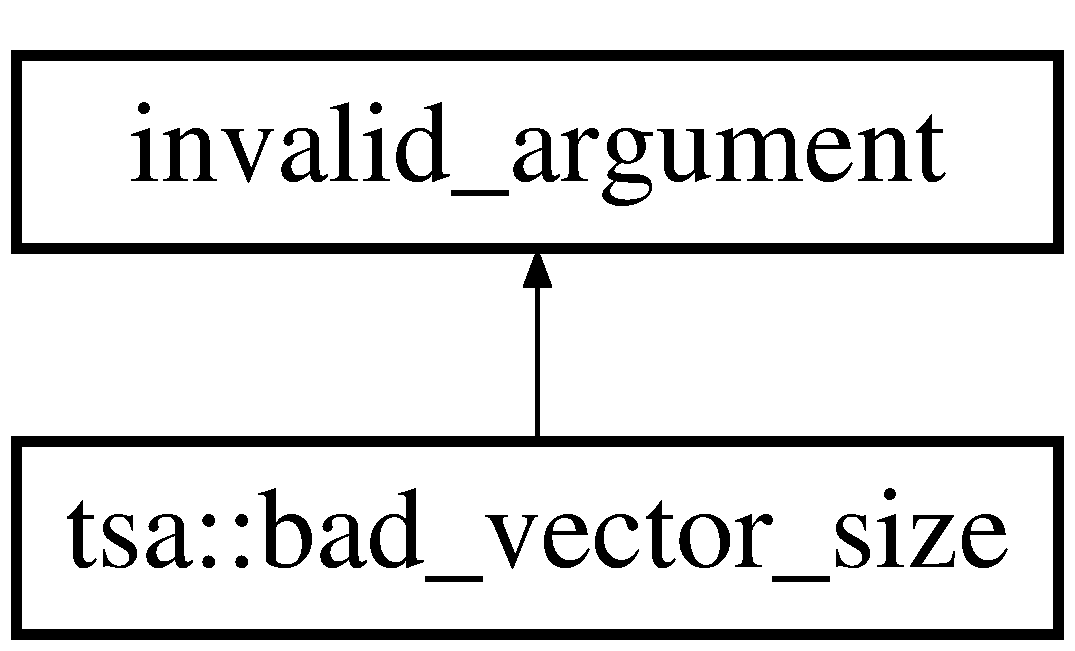
\includegraphics[height=2.000000cm]{classtsa_1_1bad__vector__size}
\end{center}
\end{figure}
\subsection*{Public Member Functions}
\begin{DoxyCompactItemize}
\item 
\hyperlink{classtsa_1_1bad__vector__size_a9ec1fb1fd91fdd191f8dfd59b51beb7a}{bad\+\_\+vector\+\_\+size} (const std\+::string \&msg)
\end{DoxyCompactItemize}


\subsection{Detailed Description}
This exception should be used when a vector argument of an algorithm has an incorrect size. It contains information about the correct expected size. 

Definition at line 98 of file Algo\+Exceptions.\+hpp.



\subsection{Constructor \& Destructor Documentation}
\mbox{\Hypertarget{classtsa_1_1bad__vector__size_a9ec1fb1fd91fdd191f8dfd59b51beb7a}\label{classtsa_1_1bad__vector__size_a9ec1fb1fd91fdd191f8dfd59b51beb7a}} 
\index{tsa\+::bad\+\_\+vector\+\_\+size@{tsa\+::bad\+\_\+vector\+\_\+size}!bad\+\_\+vector\+\_\+size@{bad\+\_\+vector\+\_\+size}}
\index{bad\+\_\+vector\+\_\+size@{bad\+\_\+vector\+\_\+size}!tsa\+::bad\+\_\+vector\+\_\+size@{tsa\+::bad\+\_\+vector\+\_\+size}}
\subsubsection{\texorpdfstring{bad\+\_\+vector\+\_\+size()}{bad\_vector\_size()}}
{\footnotesize\ttfamily tsa\+::bad\+\_\+vector\+\_\+size\+::bad\+\_\+vector\+\_\+size (\begin{DoxyParamCaption}\item[{const std\+::string \&}]{msg }\end{DoxyParamCaption})\hspace{0.3cm}{\ttfamily [inline]}}

Constructor


\begin{DoxyParams}{Parameters}
{\em msg} & error message \\
\hline
\end{DoxyParams}


Definition at line 106 of file Algo\+Exceptions.\+hpp.



The documentation for this class was generated from the following file\+:\begin{DoxyCompactItemize}
\item 
/home/filip/\+Ph\+D/\+W\+D\+F\+Pipe\+\_\+test/p4\+T\+S\+A/include/\hyperlink{_algo_exceptions_8hpp}{Algo\+Exceptions.\+hpp}\end{DoxyCompactItemize}

\hypertarget{classtsa_1_1_bartlett_window}{}\section{tsa\+:\+:Bartlett\+Window Class Reference}
\label{classtsa_1_1_bartlett_window}\index{tsa\+::\+Bartlett\+Window@{tsa\+::\+Bartlett\+Window}}


Bartlett windowing algorithm.  




{\ttfamily \#include $<$Bartlett\+Window.\+hpp$>$}

Inheritance diagram for tsa\+:\+:Bartlett\+Window\+:\begin{figure}[H]
\begin{center}
\leavevmode
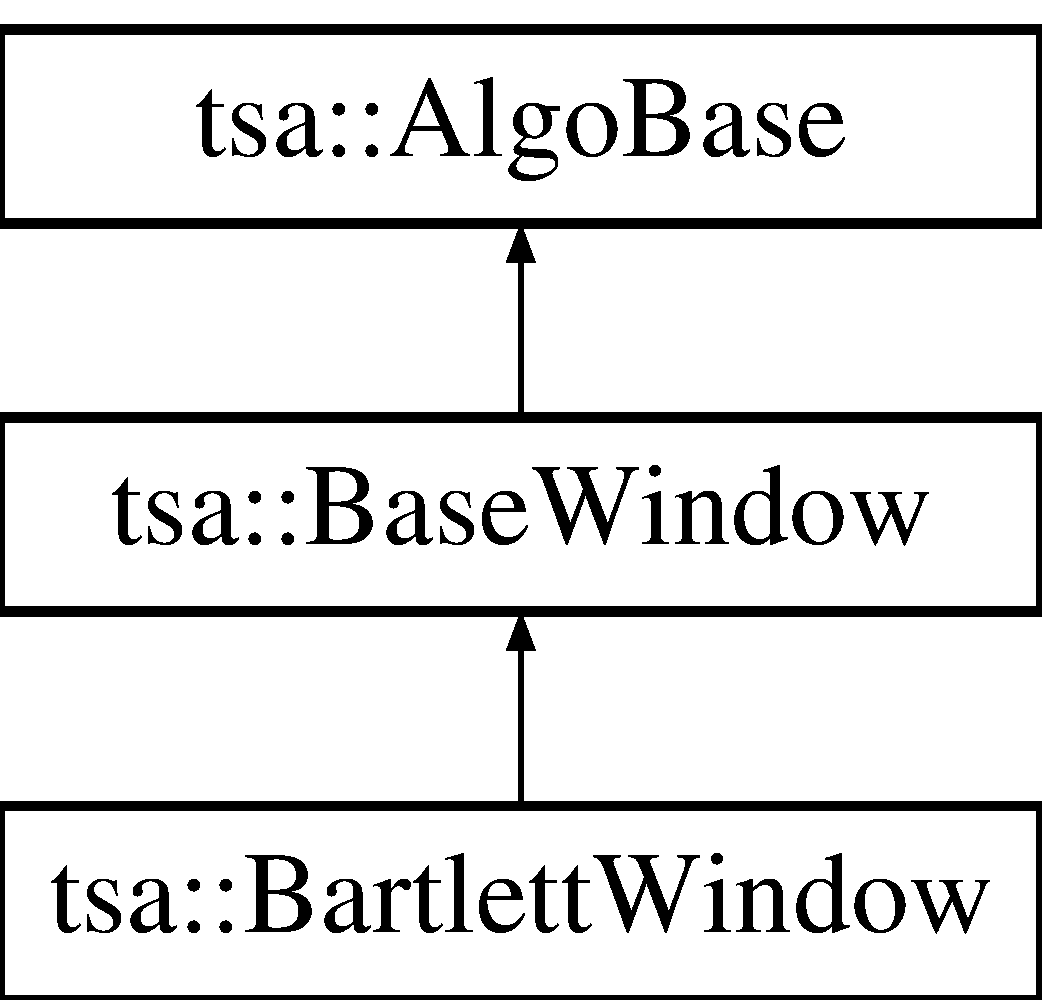
\includegraphics[height=3.000000cm]{classtsa_1_1_bartlett_window}
\end{center}
\end{figure}
\subsection*{Public Member Functions}
\begin{DoxyCompactItemize}
\item 
\hyperlink{classtsa_1_1_bartlett_window_a9177fa400660b6bdecfcecbfbffeedbe}{Bartlett\+Window} (int size)
\item 
\hyperlink{classtsa_1_1_bartlett_window_a9da0612e0081996ef30439403a8a9c87}{Bartlett\+Window} (int size, const std\+::string \&)
\item 
virtual \hyperlink{classtsa_1_1_bartlett_window_a45ce87f449514520865841aa3ac0abac}{$\sim$\+Bartlett\+Window} ()
\end{DoxyCompactItemize}
\begin{Indent}\textbf{ Operations}\par
\begin{DoxyCompactItemize}
\item 
void \hyperlink{classtsa_1_1_bartlett_window_a9bad239fb8fbaa295713c904e3d9d92e}{operator()} (\hyperlink{namespacetsa_ac599574bcc094eda25613724b8f3ca9e}{Seq\+View\+Double} \&v1)
\item 
void \hyperlink{classtsa_1_1_bartlett_window_a44d722552ca5281e28a28eadbed2099e}{operator()} (\hyperlink{namespacetsa_ac599574bcc094eda25613724b8f3ca9e}{Seq\+View\+Double} \&v1, \hyperlink{namespacetsa_ac599574bcc094eda25613724b8f3ca9e}{Seq\+View\+Double} \&v2)
\item 
void \hyperlink{classtsa_1_1_bartlett_window_af63f6fdd7e2a10d77db1c7363e9963f5}{Resize} (unsigned int size)
\end{DoxyCompactItemize}
\end{Indent}
\subsection*{Private Member Functions}
\begin{DoxyCompactItemize}
\item 
void \hyperlink{classtsa_1_1_bartlett_window_afb3c6c8aa249db673da8dd625ffbb8a5}{Fill\+Window} ()
\end{DoxyCompactItemize}
\subsection*{Additional Inherited Members}


\subsection{Detailed Description}
Bartlett windowing algorithm. 

Definition at line 68 of file Bartlett\+Window.\+hpp.



\subsection{Constructor \& Destructor Documentation}
\mbox{\Hypertarget{classtsa_1_1_bartlett_window_a9177fa400660b6bdecfcecbfbffeedbe}\label{classtsa_1_1_bartlett_window_a9177fa400660b6bdecfcecbfbffeedbe}} 
\index{tsa\+::\+Bartlett\+Window@{tsa\+::\+Bartlett\+Window}!Bartlett\+Window@{Bartlett\+Window}}
\index{Bartlett\+Window@{Bartlett\+Window}!tsa\+::\+Bartlett\+Window@{tsa\+::\+Bartlett\+Window}}
\subsubsection{\texorpdfstring{Bartlett\+Window()}{BartlettWindow()}\hspace{0.1cm}{\footnotesize\ttfamily [1/2]}}
{\footnotesize\ttfamily tsa\+::\+Bartlett\+Window\+::\+Bartlett\+Window (\begin{DoxyParamCaption}\item[{int}]{size }\end{DoxyParamCaption})\hspace{0.3cm}{\ttfamily [inline]}}

Constructor


\begin{DoxyParams}{Parameters}
{\em size} & the size of the window \\
\hline
{\em cached} & true if the window must be preevaluated in a buffer \\
\hline
\end{DoxyParams}


Definition at line 77 of file Bartlett\+Window.\+hpp.

\mbox{\Hypertarget{classtsa_1_1_bartlett_window_a9da0612e0081996ef30439403a8a9c87}\label{classtsa_1_1_bartlett_window_a9da0612e0081996ef30439403a8a9c87}} 
\index{tsa\+::\+Bartlett\+Window@{tsa\+::\+Bartlett\+Window}!Bartlett\+Window@{Bartlett\+Window}}
\index{Bartlett\+Window@{Bartlett\+Window}!tsa\+::\+Bartlett\+Window@{tsa\+::\+Bartlett\+Window}}
\subsubsection{\texorpdfstring{Bartlett\+Window()}{BartlettWindow()}\hspace{0.1cm}{\footnotesize\ttfamily [2/2]}}
{\footnotesize\ttfamily tsa\+::\+Bartlett\+Window\+::\+Bartlett\+Window (\begin{DoxyParamCaption}\item[{int}]{size,  }\item[{const std\+::string \&}]{ }\end{DoxyParamCaption})\hspace{0.3cm}{\ttfamily [inline]}}



Definition at line 83 of file Bartlett\+Window.\+hpp.

\mbox{\Hypertarget{classtsa_1_1_bartlett_window_a45ce87f449514520865841aa3ac0abac}\label{classtsa_1_1_bartlett_window_a45ce87f449514520865841aa3ac0abac}} 
\index{tsa\+::\+Bartlett\+Window@{tsa\+::\+Bartlett\+Window}!````~Bartlett\+Window@{$\sim$\+Bartlett\+Window}}
\index{````~Bartlett\+Window@{$\sim$\+Bartlett\+Window}!tsa\+::\+Bartlett\+Window@{tsa\+::\+Bartlett\+Window}}
\subsubsection{\texorpdfstring{$\sim$\+Bartlett\+Window()}{~BartlettWindow()}}
{\footnotesize\ttfamily virtual tsa\+::\+Bartlett\+Window\+::$\sim$\+Bartlett\+Window (\begin{DoxyParamCaption}{ }\end{DoxyParamCaption})\hspace{0.3cm}{\ttfamily [inline]}, {\ttfamily [virtual]}}

Destructor 

Definition at line 92 of file Bartlett\+Window.\+hpp.



\subsection{Member Function Documentation}
\mbox{\Hypertarget{classtsa_1_1_bartlett_window_afb3c6c8aa249db673da8dd625ffbb8a5}\label{classtsa_1_1_bartlett_window_afb3c6c8aa249db673da8dd625ffbb8a5}} 
\index{tsa\+::\+Bartlett\+Window@{tsa\+::\+Bartlett\+Window}!Fill\+Window@{Fill\+Window}}
\index{Fill\+Window@{Fill\+Window}!tsa\+::\+Bartlett\+Window@{tsa\+::\+Bartlett\+Window}}
\subsubsection{\texorpdfstring{Fill\+Window()}{FillWindow()}}
{\footnotesize\ttfamily void tsa\+::\+Bartlett\+Window\+::\+Fill\+Window (\begin{DoxyParamCaption}{ }\end{DoxyParamCaption})\hspace{0.3cm}{\ttfamily [inline]}, {\ttfamily [private]}, {\ttfamily [virtual]}}

Initialize the window with the correct values, given its actual size. This is a pure virtual function, which is redefined by each window class. 

Reimplemented from \hyperlink{classtsa_1_1_base_window_aa74b29105d94caa521d308198e8e6643}{tsa\+::\+Base\+Window}.



Definition at line 195 of file Bartlett\+Window.\+hpp.

\mbox{\Hypertarget{classtsa_1_1_bartlett_window_a9bad239fb8fbaa295713c904e3d9d92e}\label{classtsa_1_1_bartlett_window_a9bad239fb8fbaa295713c904e3d9d92e}} 
\index{tsa\+::\+Bartlett\+Window@{tsa\+::\+Bartlett\+Window}!operator()@{operator()}}
\index{operator()@{operator()}!tsa\+::\+Bartlett\+Window@{tsa\+::\+Bartlett\+Window}}
\subsubsection{\texorpdfstring{operator()()}{operator()()}\hspace{0.1cm}{\footnotesize\ttfamily [1/2]}}
{\footnotesize\ttfamily void tsa\+::\+Bartlett\+Window\+::operator() (\begin{DoxyParamCaption}\item[{\hyperlink{namespacetsa_ac599574bcc094eda25613724b8f3ca9e}{Seq\+View\+Double} \&}]{v1 }\end{DoxyParamCaption})\hspace{0.3cm}{\ttfamily [inline]}, {\ttfamily [virtual]}}

Apply the window to a given time view.


\begin{DoxyParams}{Parameters}
{\em v1} & the time view \\
\hline
\end{DoxyParams}


Reimplemented from \hyperlink{classtsa_1_1_base_window_a05d9edb95dc01840a1b2df78dfa3a8c1}{tsa\+::\+Base\+Window}.



Definition at line 106 of file Bartlett\+Window.\+hpp.

\mbox{\Hypertarget{classtsa_1_1_bartlett_window_a44d722552ca5281e28a28eadbed2099e}\label{classtsa_1_1_bartlett_window_a44d722552ca5281e28a28eadbed2099e}} 
\index{tsa\+::\+Bartlett\+Window@{tsa\+::\+Bartlett\+Window}!operator()@{operator()}}
\index{operator()@{operator()}!tsa\+::\+Bartlett\+Window@{tsa\+::\+Bartlett\+Window}}
\subsubsection{\texorpdfstring{operator()()}{operator()()}\hspace{0.1cm}{\footnotesize\ttfamily [2/2]}}
{\footnotesize\ttfamily void tsa\+::\+Bartlett\+Window\+::operator() (\begin{DoxyParamCaption}\item[{\hyperlink{namespacetsa_ac599574bcc094eda25613724b8f3ca9e}{Seq\+View\+Double} \&}]{v1,  }\item[{\hyperlink{namespacetsa_ac599574bcc094eda25613724b8f3ca9e}{Seq\+View\+Double} \&}]{v2 }\end{DoxyParamCaption})\hspace{0.3cm}{\ttfamily [inline]}, {\ttfamily [virtual]}}

Apply a window to an input view and write the results on a output view.


\begin{DoxyParams}{Parameters}
{\em v1} & the input view \\
\hline
{\em v2} & the output view \\
\hline
\end{DoxyParams}


Reimplemented from \hyperlink{classtsa_1_1_base_window_afda50daa943527e09792b06e5ba69bcb}{tsa\+::\+Base\+Window}.



Definition at line 128 of file Bartlett\+Window.\+hpp.

\mbox{\Hypertarget{classtsa_1_1_bartlett_window_af63f6fdd7e2a10d77db1c7363e9963f5}\label{classtsa_1_1_bartlett_window_af63f6fdd7e2a10d77db1c7363e9963f5}} 
\index{tsa\+::\+Bartlett\+Window@{tsa\+::\+Bartlett\+Window}!Resize@{Resize}}
\index{Resize@{Resize}!tsa\+::\+Bartlett\+Window@{tsa\+::\+Bartlett\+Window}}
\subsubsection{\texorpdfstring{Resize()}{Resize()}}
{\footnotesize\ttfamily void tsa\+::\+Bartlett\+Window\+::\+Resize (\begin{DoxyParamCaption}\item[{unsigned int}]{size }\end{DoxyParamCaption})\hspace{0.3cm}{\ttfamily [inline]}, {\ttfamily [virtual]}}

Resize the window dimension.


\begin{DoxyParams}{Parameters}
{\em size} & new size for the window \\
\hline
\end{DoxyParams}


Reimplemented from \hyperlink{classtsa_1_1_base_window_a8a2a3425f2915762d50fa57dd0e04f22}{tsa\+::\+Base\+Window}.



Definition at line 157 of file Bartlett\+Window.\+hpp.



The documentation for this class was generated from the following file\+:\begin{DoxyCompactItemize}
\item 
/home/filip/\+Ph\+D/\+W\+D\+F\+Pipe\+\_\+test/p4\+T\+S\+A/include/\hyperlink{_bartlett_window_8hpp}{Bartlett\+Window.\+hpp}\end{DoxyCompactItemize}

\hypertarget{classtsa_1_1_base_f_f_t}{}\section{tsa\+:\+:Base\+F\+FT Class Reference}
\label{classtsa_1_1_base_f_f_t}\index{tsa\+::\+Base\+F\+FT@{tsa\+::\+Base\+F\+FT}}


Base class for various F\+FT.  




{\ttfamily \#include $<$Base\+F\+F\+T.\+hpp$>$}

Inheritance diagram for tsa\+:\+:Base\+F\+FT\+:\begin{figure}[H]
\begin{center}
\leavevmode
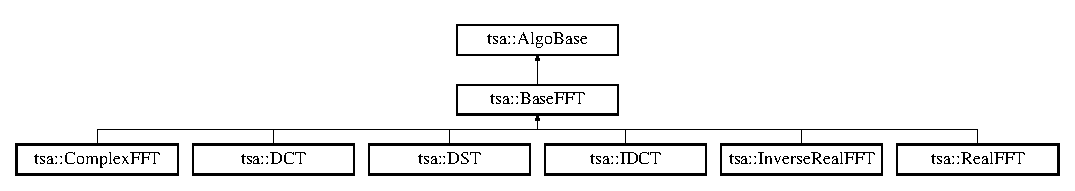
\includegraphics[height=2.121212cm]{classtsa_1_1_base_f_f_t}
\end{center}
\end{figure}
\subsection*{Public Member Functions}
\begin{DoxyCompactItemize}
\item 
\hyperlink{classtsa_1_1_base_f_f_t_a724f59f3f5bded31174373eac81e67ee}{Base\+F\+FT} (int size, enum \hyperlink{namespacetsa_a217e07ef78939f88b22c8428ac96b1ae}{F\+F\+T\+Planning\+Mode} mode, bool Preserve\+Input)
\item 
\hyperlink{classtsa_1_1_base_f_f_t_a84fa441e825a8e375f9721263d358ac8}{Base\+F\+FT} (const \hyperlink{classtsa_1_1_base_f_f_t}{Base\+F\+FT} \&from)
\item 
virtual \hyperlink{classtsa_1_1_base_f_f_t_ad73b78693c83ef6c7e07701965ae8cb6}{$\sim$\+Base\+F\+FT} ()
\end{DoxyCompactItemize}
\begin{Indent}\textbf{ Setters}\par
\begin{DoxyCompactItemize}
\item 
void \hyperlink{classtsa_1_1_base_f_f_t_a4a8b00feb20dc3ace768d3c851143a03}{Set\+Planning\+Mode} (enum \hyperlink{namespacetsa_a217e07ef78939f88b22c8428ac96b1ae}{F\+F\+T\+Planning\+Mode} mode)
\item 
void \hyperlink{classtsa_1_1_base_f_f_t_a5b1e2f36dbdfe197aa6c74d1cf963f40}{Set\+Preserve\+Input} (bool flag=true)
\end{DoxyCompactItemize}
\end{Indent}
\subsection*{Protected Attributes}
\begin{DoxyCompactItemize}
\item 
fftw\+\_\+plan \hyperlink{classtsa_1_1_base_f_f_t_a5c7dd6dee349547018d493be6d5874eb}{m\+Plan}
\item 
bool \hyperlink{classtsa_1_1_base_f_f_t_aa89fef1777c6df148cdb8533265b6163}{m\+Plan\+Needs\+Update}
\item 
unsigned int \hyperlink{classtsa_1_1_base_f_f_t_a171c71011fea314f23633b1816771d98}{m\+Logical\+Size}
\item 
unsigned int \hyperlink{classtsa_1_1_base_f_f_t_abbd656cda5a7cb6a88fc5d556d3269f7}{m\+Planning\+Rigor}
\item 
unsigned int \hyperlink{classtsa_1_1_base_f_f_t_a2fe7f53db024bb408beeb5e22eaefbb9}{m\+Planning\+Restriction}
\end{DoxyCompactItemize}
\subsection*{Operations}
\begin{DoxyCompactItemize}
\item 
virtual void \hyperlink{classtsa_1_1_base_f_f_t_a9af0c36413173821cac8dbdce9cfe3b4}{Make\+Plan} ()=0
\item 
static void \hyperlink{classtsa_1_1_base_f_f_t_a1f5332f508749018f0c6a58c9b1ed9dc}{Save\+Wisdom\+On\+File} (std\+::string filename)
\item 
static void \hyperlink{classtsa_1_1_base_f_f_t_a53ccc1ae425bb9f91adbd5562ecb9131}{Load\+Wisdom\+From\+File} (std\+::string filename)
\item 
static void \hyperlink{classtsa_1_1_base_f_f_t_a7069819e421ad4cb2a4c58f65c8540ea}{Forget\+Wisdom} ()
\end{DoxyCompactItemize}


\subsection{Detailed Description}
Base class for various F\+FT. 

Definition at line 88 of file Base\+F\+F\+T.\+hpp.



\subsection{Constructor \& Destructor Documentation}
\mbox{\Hypertarget{classtsa_1_1_base_f_f_t_a724f59f3f5bded31174373eac81e67ee}\label{classtsa_1_1_base_f_f_t_a724f59f3f5bded31174373eac81e67ee}} 
\index{tsa\+::\+Base\+F\+FT@{tsa\+::\+Base\+F\+FT}!Base\+F\+FT@{Base\+F\+FT}}
\index{Base\+F\+FT@{Base\+F\+FT}!tsa\+::\+Base\+F\+FT@{tsa\+::\+Base\+F\+FT}}
\subsubsection{\texorpdfstring{Base\+F\+F\+T()}{BaseFFT()}\hspace{0.1cm}{\footnotesize\ttfamily [1/2]}}
{\footnotesize\ttfamily tsa\+::\+Base\+F\+F\+T\+::\+Base\+F\+FT (\begin{DoxyParamCaption}\item[{int}]{size,  }\item[{enum \hyperlink{namespacetsa_a217e07ef78939f88b22c8428ac96b1ae}{F\+F\+T\+Planning\+Mode}}]{mode,  }\item[{bool}]{Preserve\+Input }\end{DoxyParamCaption})\hspace{0.3cm}{\ttfamily [inline]}}

Constructor


\begin{DoxyParams}{Parameters}
{\em size} & the size of the transform \\
\hline
{\em mode} & specify the way in which plans are calculated \\
\hline
{\em Preserve\+Input} & true if the input buffer must be preserved during the transform, false otherwise \\
\hline
\end{DoxyParams}


Definition at line 98 of file Base\+F\+F\+T.\+hpp.

\mbox{\Hypertarget{classtsa_1_1_base_f_f_t_a84fa441e825a8e375f9721263d358ac8}\label{classtsa_1_1_base_f_f_t_a84fa441e825a8e375f9721263d358ac8}} 
\index{tsa\+::\+Base\+F\+FT@{tsa\+::\+Base\+F\+FT}!Base\+F\+FT@{Base\+F\+FT}}
\index{Base\+F\+FT@{Base\+F\+FT}!tsa\+::\+Base\+F\+FT@{tsa\+::\+Base\+F\+FT}}
\subsubsection{\texorpdfstring{Base\+F\+F\+T()}{BaseFFT()}\hspace{0.1cm}{\footnotesize\ttfamily [2/2]}}
{\footnotesize\ttfamily tsa\+::\+Base\+F\+F\+T\+::\+Base\+F\+FT (\begin{DoxyParamCaption}\item[{const \hyperlink{classtsa_1_1_base_f_f_t}{Base\+F\+FT} \&}]{from }\end{DoxyParamCaption})\hspace{0.3cm}{\ttfamily [inline]}}

Copy constructor


\begin{DoxyParams}{Parameters}
{\em from} & The instance that must be copied \\
\hline
\end{DoxyParams}


Definition at line 111 of file Base\+F\+F\+T.\+hpp.

\mbox{\Hypertarget{classtsa_1_1_base_f_f_t_ad73b78693c83ef6c7e07701965ae8cb6}\label{classtsa_1_1_base_f_f_t_ad73b78693c83ef6c7e07701965ae8cb6}} 
\index{tsa\+::\+Base\+F\+FT@{tsa\+::\+Base\+F\+FT}!````~Base\+F\+FT@{$\sim$\+Base\+F\+FT}}
\index{````~Base\+F\+FT@{$\sim$\+Base\+F\+FT}!tsa\+::\+Base\+F\+FT@{tsa\+::\+Base\+F\+FT}}
\subsubsection{\texorpdfstring{$\sim$\+Base\+F\+F\+T()}{~BaseFFT()}}
{\footnotesize\ttfamily virtual tsa\+::\+Base\+F\+F\+T\+::$\sim$\+Base\+F\+FT (\begin{DoxyParamCaption}{ }\end{DoxyParamCaption})\hspace{0.3cm}{\ttfamily [inline]}, {\ttfamily [virtual]}}

Destructor 

Definition at line 122 of file Base\+F\+F\+T.\+hpp.



\subsection{Member Function Documentation}
\mbox{\Hypertarget{classtsa_1_1_base_f_f_t_a7069819e421ad4cb2a4c58f65c8540ea}\label{classtsa_1_1_base_f_f_t_a7069819e421ad4cb2a4c58f65c8540ea}} 
\index{tsa\+::\+Base\+F\+FT@{tsa\+::\+Base\+F\+FT}!Forget\+Wisdom@{Forget\+Wisdom}}
\index{Forget\+Wisdom@{Forget\+Wisdom}!tsa\+::\+Base\+F\+FT@{tsa\+::\+Base\+F\+FT}}
\subsubsection{\texorpdfstring{Forget\+Wisdom()}{ForgetWisdom()}}
{\footnotesize\ttfamily static void tsa\+::\+Base\+F\+F\+T\+::\+Forget\+Wisdom (\begin{DoxyParamCaption}{ }\end{DoxyParamCaption})\hspace{0.3cm}{\ttfamily [inline]}, {\ttfamily [static]}}

Forget wisdom 

Definition at line 166 of file Base\+F\+F\+T.\+hpp.

\mbox{\Hypertarget{classtsa_1_1_base_f_f_t_a53ccc1ae425bb9f91adbd5562ecb9131}\label{classtsa_1_1_base_f_f_t_a53ccc1ae425bb9f91adbd5562ecb9131}} 
\index{tsa\+::\+Base\+F\+FT@{tsa\+::\+Base\+F\+FT}!Load\+Wisdom\+From\+File@{Load\+Wisdom\+From\+File}}
\index{Load\+Wisdom\+From\+File@{Load\+Wisdom\+From\+File}!tsa\+::\+Base\+F\+FT@{tsa\+::\+Base\+F\+FT}}
\subsubsection{\texorpdfstring{Load\+Wisdom\+From\+File()}{LoadWisdomFromFile()}}
{\footnotesize\ttfamily static void tsa\+::\+Base\+F\+F\+T\+::\+Load\+Wisdom\+From\+File (\begin{DoxyParamCaption}\item[{std\+::string}]{filename }\end{DoxyParamCaption})\hspace{0.3cm}{\ttfamily [inline]}, {\ttfamily [static]}}

Load the actual wisdom for plan generation from a file


\begin{DoxyParams}{Parameters}
{\em filename} & the name of the file \\
\hline
\end{DoxyParams}


Definition at line 152 of file Base\+F\+F\+T.\+hpp.

\mbox{\Hypertarget{classtsa_1_1_base_f_f_t_a9af0c36413173821cac8dbdce9cfe3b4}\label{classtsa_1_1_base_f_f_t_a9af0c36413173821cac8dbdce9cfe3b4}} 
\index{tsa\+::\+Base\+F\+FT@{tsa\+::\+Base\+F\+FT}!Make\+Plan@{Make\+Plan}}
\index{Make\+Plan@{Make\+Plan}!tsa\+::\+Base\+F\+FT@{tsa\+::\+Base\+F\+FT}}
\subsubsection{\texorpdfstring{Make\+Plan()}{MakePlan()}}
{\footnotesize\ttfamily virtual void tsa\+::\+Base\+F\+F\+T\+::\+Make\+Plan (\begin{DoxyParamCaption}{ }\end{DoxyParamCaption})\hspace{0.3cm}{\ttfamily [pure virtual]}}

Make a new plan, with the current parameters. 

Implemented in \hyperlink{classtsa_1_1_real_f_f_t_a6684b1abf6f9de2d7c546c3556ef0a0e}{tsa\+::\+Real\+F\+FT}, \hyperlink{classtsa_1_1_inverse_real_f_f_t_ae5b45701f989efce89c6c336ec78c189}{tsa\+::\+Inverse\+Real\+F\+FT}, \hyperlink{classtsa_1_1_d_c_t_a2d24c07a7b3f96b16056eee1ab9bad89}{tsa\+::\+D\+CT}, \hyperlink{classtsa_1_1_d_s_t_a066a93f3ddbf56f8e5c67067156ebb9a}{tsa\+::\+D\+ST}, \hyperlink{classtsa_1_1_i_d_c_t_a3add06359e79507105820496b324ad7a}{tsa\+::\+I\+D\+CT}, and \hyperlink{classtsa_1_1_complex_f_f_t_a05acda3ab3fbb2ead70421e587cdd210}{tsa\+::\+Complex\+F\+FT}.

\mbox{\Hypertarget{classtsa_1_1_base_f_f_t_a1f5332f508749018f0c6a58c9b1ed9dc}\label{classtsa_1_1_base_f_f_t_a1f5332f508749018f0c6a58c9b1ed9dc}} 
\index{tsa\+::\+Base\+F\+FT@{tsa\+::\+Base\+F\+FT}!Save\+Wisdom\+On\+File@{Save\+Wisdom\+On\+File}}
\index{Save\+Wisdom\+On\+File@{Save\+Wisdom\+On\+File}!tsa\+::\+Base\+F\+FT@{tsa\+::\+Base\+F\+FT}}
\subsubsection{\texorpdfstring{Save\+Wisdom\+On\+File()}{SaveWisdomOnFile()}}
{\footnotesize\ttfamily static void tsa\+::\+Base\+F\+F\+T\+::\+Save\+Wisdom\+On\+File (\begin{DoxyParamCaption}\item[{std\+::string}]{filename }\end{DoxyParamCaption})\hspace{0.3cm}{\ttfamily [inline]}, {\ttfamily [static]}}

Save the actual wisdom for plan generation on a file


\begin{DoxyParams}{Parameters}
{\em filename} & the name of the file \\
\hline
\end{DoxyParams}


Definition at line 138 of file Base\+F\+F\+T.\+hpp.

\mbox{\Hypertarget{classtsa_1_1_base_f_f_t_a4a8b00feb20dc3ace768d3c851143a03}\label{classtsa_1_1_base_f_f_t_a4a8b00feb20dc3ace768d3c851143a03}} 
\index{tsa\+::\+Base\+F\+FT@{tsa\+::\+Base\+F\+FT}!Set\+Planning\+Mode@{Set\+Planning\+Mode}}
\index{Set\+Planning\+Mode@{Set\+Planning\+Mode}!tsa\+::\+Base\+F\+FT@{tsa\+::\+Base\+F\+FT}}
\subsubsection{\texorpdfstring{Set\+Planning\+Mode()}{SetPlanningMode()}}
{\footnotesize\ttfamily void tsa\+::\+Base\+F\+F\+T\+::\+Set\+Planning\+Mode (\begin{DoxyParamCaption}\item[{enum \hyperlink{namespacetsa_a217e07ef78939f88b22c8428ac96b1ae}{F\+F\+T\+Planning\+Mode}}]{mode }\end{DoxyParamCaption})\hspace{0.3cm}{\ttfamily [inline]}}

Set the way in which the plan is constructed. No new plan is generated.


\begin{DoxyParams}{Parameters}
{\em mode} & the requested planning mode. \\
\hline
\end{DoxyParams}


Definition at line 196 of file Base\+F\+F\+T.\+hpp.

\mbox{\Hypertarget{classtsa_1_1_base_f_f_t_a5b1e2f36dbdfe197aa6c74d1cf963f40}\label{classtsa_1_1_base_f_f_t_a5b1e2f36dbdfe197aa6c74d1cf963f40}} 
\index{tsa\+::\+Base\+F\+FT@{tsa\+::\+Base\+F\+FT}!Set\+Preserve\+Input@{Set\+Preserve\+Input}}
\index{Set\+Preserve\+Input@{Set\+Preserve\+Input}!tsa\+::\+Base\+F\+FT@{tsa\+::\+Base\+F\+FT}}
\subsubsection{\texorpdfstring{Set\+Preserve\+Input()}{SetPreserveInput()}}
{\footnotesize\ttfamily void tsa\+::\+Base\+F\+F\+T\+::\+Set\+Preserve\+Input (\begin{DoxyParamCaption}\item[{bool}]{flag = {\ttfamily true} }\end{DoxyParamCaption})\hspace{0.3cm}{\ttfamily [inline]}}

Request that the input buffer is preserved during the transformation. No new plan is generated.


\begin{DoxyParams}{Parameters}
{\em flag} & true (default) if input buffer must be preserved, false otherwise \\
\hline
\end{DoxyParams}


Definition at line 224 of file Base\+F\+F\+T.\+hpp.



\subsection{Member Data Documentation}
\mbox{\Hypertarget{classtsa_1_1_base_f_f_t_a171c71011fea314f23633b1816771d98}\label{classtsa_1_1_base_f_f_t_a171c71011fea314f23633b1816771d98}} 
\index{tsa\+::\+Base\+F\+FT@{tsa\+::\+Base\+F\+FT}!m\+Logical\+Size@{m\+Logical\+Size}}
\index{m\+Logical\+Size@{m\+Logical\+Size}!tsa\+::\+Base\+F\+FT@{tsa\+::\+Base\+F\+FT}}
\subsubsection{\texorpdfstring{m\+Logical\+Size}{mLogicalSize}}
{\footnotesize\ttfamily unsigned int tsa\+::\+Base\+F\+F\+T\+::m\+Logical\+Size\hspace{0.3cm}{\ttfamily [protected]}}

The size of the current plan 

Definition at line 257 of file Base\+F\+F\+T.\+hpp.

\mbox{\Hypertarget{classtsa_1_1_base_f_f_t_a5c7dd6dee349547018d493be6d5874eb}\label{classtsa_1_1_base_f_f_t_a5c7dd6dee349547018d493be6d5874eb}} 
\index{tsa\+::\+Base\+F\+FT@{tsa\+::\+Base\+F\+FT}!m\+Plan@{m\+Plan}}
\index{m\+Plan@{m\+Plan}!tsa\+::\+Base\+F\+FT@{tsa\+::\+Base\+F\+FT}}
\subsubsection{\texorpdfstring{m\+Plan}{mPlan}}
{\footnotesize\ttfamily fftw\+\_\+plan tsa\+::\+Base\+F\+F\+T\+::m\+Plan\hspace{0.3cm}{\ttfamily [protected]}}

The current plan, or N\+U\+LL if no plan is available 

Definition at line 247 of file Base\+F\+F\+T.\+hpp.

\mbox{\Hypertarget{classtsa_1_1_base_f_f_t_aa89fef1777c6df148cdb8533265b6163}\label{classtsa_1_1_base_f_f_t_aa89fef1777c6df148cdb8533265b6163}} 
\index{tsa\+::\+Base\+F\+FT@{tsa\+::\+Base\+F\+FT}!m\+Plan\+Needs\+Update@{m\+Plan\+Needs\+Update}}
\index{m\+Plan\+Needs\+Update@{m\+Plan\+Needs\+Update}!tsa\+::\+Base\+F\+FT@{tsa\+::\+Base\+F\+FT}}
\subsubsection{\texorpdfstring{m\+Plan\+Needs\+Update}{mPlanNeedsUpdate}}
{\footnotesize\ttfamily bool tsa\+::\+Base\+F\+F\+T\+::m\+Plan\+Needs\+Update\hspace{0.3cm}{\ttfamily [protected]}}

Flag\+: a parameter is changed and plan needs to be updated 

Definition at line 252 of file Base\+F\+F\+T.\+hpp.

\mbox{\Hypertarget{classtsa_1_1_base_f_f_t_a2fe7f53db024bb408beeb5e22eaefbb9}\label{classtsa_1_1_base_f_f_t_a2fe7f53db024bb408beeb5e22eaefbb9}} 
\index{tsa\+::\+Base\+F\+FT@{tsa\+::\+Base\+F\+FT}!m\+Planning\+Restriction@{m\+Planning\+Restriction}}
\index{m\+Planning\+Restriction@{m\+Planning\+Restriction}!tsa\+::\+Base\+F\+FT@{tsa\+::\+Base\+F\+FT}}
\subsubsection{\texorpdfstring{m\+Planning\+Restriction}{mPlanningRestriction}}
{\footnotesize\ttfamily unsigned int tsa\+::\+Base\+F\+F\+T\+::m\+Planning\+Restriction\hspace{0.3cm}{\ttfamily [protected]}}

The planning restriction flag. 

Definition at line 267 of file Base\+F\+F\+T.\+hpp.

\mbox{\Hypertarget{classtsa_1_1_base_f_f_t_abbd656cda5a7cb6a88fc5d556d3269f7}\label{classtsa_1_1_base_f_f_t_abbd656cda5a7cb6a88fc5d556d3269f7}} 
\index{tsa\+::\+Base\+F\+FT@{tsa\+::\+Base\+F\+FT}!m\+Planning\+Rigor@{m\+Planning\+Rigor}}
\index{m\+Planning\+Rigor@{m\+Planning\+Rigor}!tsa\+::\+Base\+F\+FT@{tsa\+::\+Base\+F\+FT}}
\subsubsection{\texorpdfstring{m\+Planning\+Rigor}{mPlanningRigor}}
{\footnotesize\ttfamily unsigned int tsa\+::\+Base\+F\+F\+T\+::m\+Planning\+Rigor\hspace{0.3cm}{\ttfamily [protected]}}

The planning mode flag 

Definition at line 262 of file Base\+F\+F\+T.\+hpp.



The documentation for this class was generated from the following file\+:\begin{DoxyCompactItemize}
\item 
/home/filip/\+Ph\+D/\+W\+D\+F\+Pipe\+\_\+test/p4\+T\+S\+A/include/\hyperlink{_base_f_f_t_8hpp}{Base\+F\+F\+T.\+hpp}\end{DoxyCompactItemize}

\hypertarget{classtsa_1_1_base_view}{}\section{tsa\+:\+:Base\+View Class Reference}
\label{classtsa_1_1_base_view}\index{tsa\+::\+Base\+View@{tsa\+::\+Base\+View}}


{\ttfamily \#include $<$Base\+View.\+hpp$>$}

Inheritance diagram for tsa\+:\+:Base\+View\+:\begin{figure}[H]
\begin{center}
\leavevmode
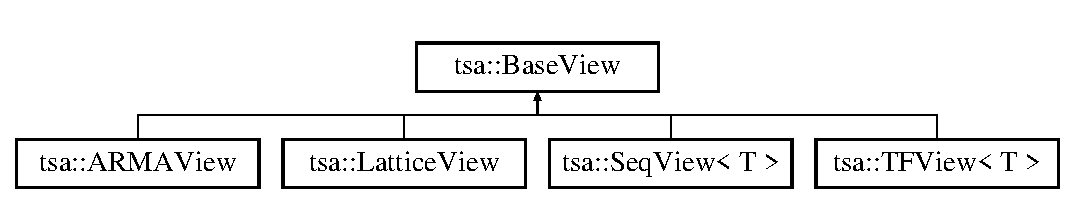
\includegraphics[height=2.000000cm]{classtsa_1_1_base_view}
\end{center}
\end{figure}
\subsection*{Public Member Functions}
\begin{DoxyCompactItemize}
\item 
\hyperlink{classtsa_1_1_base_view_a87ba8f0c139190b95f8b1c5486b342d1}{Base\+View} (const std\+::string \&a\+Name=std\+::string())
\item 
\hyperlink{classtsa_1_1_base_view_a21d825daa5ede62830f69e0ea7275008}{Base\+View} (const \hyperlink{classtsa_1_1_base_view}{Base\+View} \&from)
\item 
\hyperlink{classtsa_1_1_base_view_ad3e2d3032a8efe2bd2dc7a9a9c7636d6}{$\sim$\+Base\+View} ()
\item 
\hyperlink{classtsa_1_1_base_view}{Base\+View} \& \hyperlink{classtsa_1_1_base_view_a29e213aae81ad55e146a5e41ad5a1ce9}{operator=} (const \hyperlink{classtsa_1_1_base_view}{Base\+View} \&from)
\end{DoxyCompactItemize}
\begin{Indent}\textbf{ Getters}\par
\begin{DoxyCompactItemize}
\item 
std\+::string \hyperlink{classtsa_1_1_base_view_ac6e0354eb1ec24205ff893440ff561b9}{Get\+Name} ()
\end{DoxyCompactItemize}
\end{Indent}
\begin{Indent}\textbf{ Setters}\par
\begin{DoxyCompactItemize}
\item 
void \hyperlink{classtsa_1_1_base_view_abcfce2c227a5826093e7cb86a02765f9}{Set\+Name} (const std\+::string \&a\+Name)
\end{DoxyCompactItemize}
\end{Indent}
\subsection*{Protected Attributes}
\begin{DoxyCompactItemize}
\item 
std\+::string \hyperlink{classtsa_1_1_base_view_a91429dee1249c140160bfca20e783019}{m\+Name}
\end{DoxyCompactItemize}
\subsection*{Friends}
\begin{DoxyCompactItemize}
\item 
class \hyperlink{classtsa_1_1_base_view_af7b68757603d571922c4e3cce401ec9f}{Algo\+Base}
\end{DoxyCompactItemize}


\subsection{Detailed Description}


Definition at line 73 of file Base\+View.\+hpp.



\subsection{Constructor \& Destructor Documentation}
\mbox{\Hypertarget{classtsa_1_1_base_view_a87ba8f0c139190b95f8b1c5486b342d1}\label{classtsa_1_1_base_view_a87ba8f0c139190b95f8b1c5486b342d1}} 
\index{tsa\+::\+Base\+View@{tsa\+::\+Base\+View}!Base\+View@{Base\+View}}
\index{Base\+View@{Base\+View}!tsa\+::\+Base\+View@{tsa\+::\+Base\+View}}
\subsubsection{\texorpdfstring{Base\+View()}{BaseView()}\hspace{0.1cm}{\footnotesize\ttfamily [1/2]}}
{\footnotesize\ttfamily tsa\+::\+Base\+View\+::\+Base\+View (\begin{DoxyParamCaption}\item[{const std\+::string \&}]{a\+Name = {\ttfamily std\+:\+:string()} }\end{DoxyParamCaption})\hspace{0.3cm}{\ttfamily [inline]}}

Constructor 

Definition at line 80 of file Base\+View.\+hpp.

\mbox{\Hypertarget{classtsa_1_1_base_view_a21d825daa5ede62830f69e0ea7275008}\label{classtsa_1_1_base_view_a21d825daa5ede62830f69e0ea7275008}} 
\index{tsa\+::\+Base\+View@{tsa\+::\+Base\+View}!Base\+View@{Base\+View}}
\index{Base\+View@{Base\+View}!tsa\+::\+Base\+View@{tsa\+::\+Base\+View}}
\subsubsection{\texorpdfstring{Base\+View()}{BaseView()}\hspace{0.1cm}{\footnotesize\ttfamily [2/2]}}
{\footnotesize\ttfamily tsa\+::\+Base\+View\+::\+Base\+View (\begin{DoxyParamCaption}\item[{const \hyperlink{classtsa_1_1_base_view}{Base\+View} \&}]{from }\end{DoxyParamCaption})\hspace{0.3cm}{\ttfamily [inline]}}

Copy constructor


\begin{DoxyParams}{Parameters}
{\em from} & The instance that must be copied \\
\hline
\end{DoxyParams}


Definition at line 91 of file Base\+View.\+hpp.

\mbox{\Hypertarget{classtsa_1_1_base_view_ad3e2d3032a8efe2bd2dc7a9a9c7636d6}\label{classtsa_1_1_base_view_ad3e2d3032a8efe2bd2dc7a9a9c7636d6}} 
\index{tsa\+::\+Base\+View@{tsa\+::\+Base\+View}!````~Base\+View@{$\sim$\+Base\+View}}
\index{````~Base\+View@{$\sim$\+Base\+View}!tsa\+::\+Base\+View@{tsa\+::\+Base\+View}}
\subsubsection{\texorpdfstring{$\sim$\+Base\+View()}{~BaseView()}}
{\footnotesize\ttfamily tsa\+::\+Base\+View\+::$\sim$\+Base\+View (\begin{DoxyParamCaption}{ }\end{DoxyParamCaption})\hspace{0.3cm}{\ttfamily [inline]}}

Destructor 

Definition at line 99 of file Base\+View.\+hpp.



\subsection{Member Function Documentation}
\mbox{\Hypertarget{classtsa_1_1_base_view_ac6e0354eb1ec24205ff893440ff561b9}\label{classtsa_1_1_base_view_ac6e0354eb1ec24205ff893440ff561b9}} 
\index{tsa\+::\+Base\+View@{tsa\+::\+Base\+View}!Get\+Name@{Get\+Name}}
\index{Get\+Name@{Get\+Name}!tsa\+::\+Base\+View@{tsa\+::\+Base\+View}}
\subsubsection{\texorpdfstring{Get\+Name()}{GetName()}}
{\footnotesize\ttfamily std\+::string tsa\+::\+Base\+View\+::\+Get\+Name (\begin{DoxyParamCaption}{ }\end{DoxyParamCaption})\hspace{0.3cm}{\ttfamily [inline]}}



Definition at line 129 of file Base\+View.\+hpp.

\mbox{\Hypertarget{classtsa_1_1_base_view_a29e213aae81ad55e146a5e41ad5a1ce9}\label{classtsa_1_1_base_view_a29e213aae81ad55e146a5e41ad5a1ce9}} 
\index{tsa\+::\+Base\+View@{tsa\+::\+Base\+View}!operator=@{operator=}}
\index{operator=@{operator=}!tsa\+::\+Base\+View@{tsa\+::\+Base\+View}}
\subsubsection{\texorpdfstring{operator=()}{operator=()}}
{\footnotesize\ttfamily \hyperlink{classtsa_1_1_base_view}{Base\+View}\& tsa\+::\+Base\+View\+::operator= (\begin{DoxyParamCaption}\item[{const \hyperlink{classtsa_1_1_base_view}{Base\+View} \&}]{from }\end{DoxyParamCaption})\hspace{0.3cm}{\ttfamily [inline]}}

Assignement operator


\begin{DoxyParams}{Parameters}
{\em from} & The instance to be assigned from\\
\hline
\end{DoxyParams}
\begin{DoxyReturn}{Returns}
a reference to a new object 
\end{DoxyReturn}


Definition at line 110 of file Base\+View.\+hpp.

\mbox{\Hypertarget{classtsa_1_1_base_view_abcfce2c227a5826093e7cb86a02765f9}\label{classtsa_1_1_base_view_abcfce2c227a5826093e7cb86a02765f9}} 
\index{tsa\+::\+Base\+View@{tsa\+::\+Base\+View}!Set\+Name@{Set\+Name}}
\index{Set\+Name@{Set\+Name}!tsa\+::\+Base\+View@{tsa\+::\+Base\+View}}
\subsubsection{\texorpdfstring{Set\+Name()}{SetName()}}
{\footnotesize\ttfamily void tsa\+::\+Base\+View\+::\+Set\+Name (\begin{DoxyParamCaption}\item[{const std\+::string \&}]{a\+Name }\end{DoxyParamCaption})\hspace{0.3cm}{\ttfamily [inline]}}



Definition at line 141 of file Base\+View.\+hpp.



\subsection{Friends And Related Function Documentation}
\mbox{\Hypertarget{classtsa_1_1_base_view_af7b68757603d571922c4e3cce401ec9f}\label{classtsa_1_1_base_view_af7b68757603d571922c4e3cce401ec9f}} 
\index{tsa\+::\+Base\+View@{tsa\+::\+Base\+View}!Algo\+Base@{Algo\+Base}}
\index{Algo\+Base@{Algo\+Base}!tsa\+::\+Base\+View@{tsa\+::\+Base\+View}}
\subsubsection{\texorpdfstring{Algo\+Base}{AlgoBase}}
{\footnotesize\ttfamily friend class \hyperlink{classtsa_1_1_algo_base}{Algo\+Base}\hspace{0.3cm}{\ttfamily [friend]}}



Definition at line 75 of file Base\+View.\+hpp.



\subsection{Member Data Documentation}
\mbox{\Hypertarget{classtsa_1_1_base_view_a91429dee1249c140160bfca20e783019}\label{classtsa_1_1_base_view_a91429dee1249c140160bfca20e783019}} 
\index{tsa\+::\+Base\+View@{tsa\+::\+Base\+View}!m\+Name@{m\+Name}}
\index{m\+Name@{m\+Name}!tsa\+::\+Base\+View@{tsa\+::\+Base\+View}}
\subsubsection{\texorpdfstring{m\+Name}{mName}}
{\footnotesize\ttfamily std\+::string tsa\+::\+Base\+View\+::m\+Name\hspace{0.3cm}{\ttfamily [protected]}}



Definition at line 153 of file Base\+View.\+hpp.



The documentation for this class was generated from the following file\+:\begin{DoxyCompactItemize}
\item 
/home/filip/\+Ph\+D/\+W\+D\+F\+Pipe\+\_\+test/p4\+T\+S\+A/include/\hyperlink{_base_view_8hpp}{Base\+View.\+hpp}\end{DoxyCompactItemize}

\hypertarget{classtsa_1_1_base_window}{}\section{tsa\+:\+:Base\+Window Class Reference}
\label{classtsa_1_1_base_window}\index{tsa\+::\+Base\+Window@{tsa\+::\+Base\+Window}}


Base class for various windowing algorithms.  




{\ttfamily \#include $<$Base\+Window.\+hpp$>$}

Inheritance diagram for tsa\+:\+:Base\+Window\+:\begin{figure}[H]
\begin{center}
\leavevmode
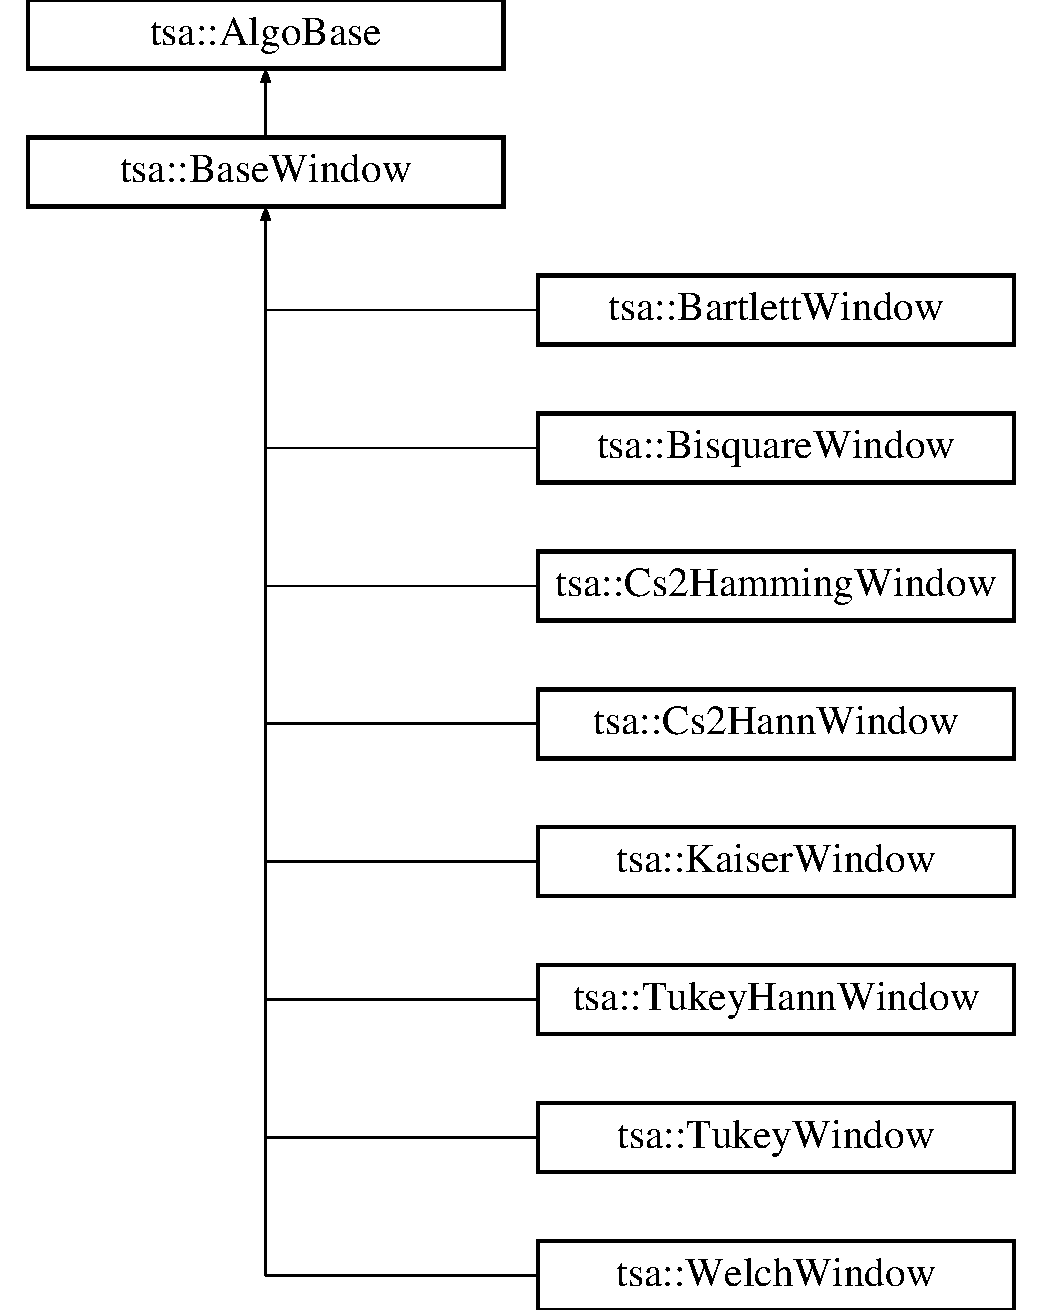
\includegraphics[height=10.000000cm]{classtsa_1_1_base_window}
\end{center}
\end{figure}
\subsection*{Public Member Functions}
\begin{DoxyCompactItemize}
\item 
\hyperlink{classtsa_1_1_base_window_aea4dee45722299896913859d7b899d6f}{Base\+Window} (unsigned int size)
\item 
virtual \hyperlink{classtsa_1_1_base_window_a0e99ffa3d84e8c7a05f7de437bfd6241}{$\sim$\+Base\+Window} ()
\item 
virtual void \hyperlink{classtsa_1_1_base_window_ad6681a5cb29414a97af6be1ea7805a81}{Normalize} ()
\end{DoxyCompactItemize}
\begin{Indent}\textbf{ Getters}\par
\begin{DoxyCompactItemize}
\item 
unsigned int \hyperlink{classtsa_1_1_base_window_af3e45daf0401f06108c6634344532af8}{Get\+Size} ()
\end{DoxyCompactItemize}
\end{Indent}
\subsection*{Protected Member Functions}
\begin{DoxyCompactItemize}
\item 
virtual void \hyperlink{classtsa_1_1_base_window_aa74b29105d94caa521d308198e8e6643}{Fill\+Window} ()
\end{DoxyCompactItemize}
\subsection*{Protected Attributes}
\begin{DoxyCompactItemize}
\item 
\hyperlink{namespacetsa_a8900fb03d849baf447a1a0efe2561fb2}{Dvector} \hyperlink{classtsa_1_1_base_window_a182b397ac3f3c409bfcb3a39d9c1575a}{m\+Window}
\end{DoxyCompactItemize}
\subsection*{Operations}
\begin{DoxyCompactItemize}
\item 
virtual void \hyperlink{classtsa_1_1_base_window_a05d9edb95dc01840a1b2df78dfa3a8c1}{operator()} (\hyperlink{namespacetsa_ac599574bcc094eda25613724b8f3ca9e}{Seq\+View\+Double} \&v1)
\item 
virtual void \hyperlink{classtsa_1_1_base_window_afda50daa943527e09792b06e5ba69bcb}{operator()} (\hyperlink{namespacetsa_ac599574bcc094eda25613724b8f3ca9e}{Seq\+View\+Double} \&v1, \hyperlink{namespacetsa_ac599574bcc094eda25613724b8f3ca9e}{Seq\+View\+Double} \&v2)
\item 
void \hyperlink{classtsa_1_1_base_window_a15647cb85344c7e82ecde50675b07efd}{execute} (\hyperlink{namespacetsa_ad260cd21c1891c4ed391fe788569aba4}{Dmatrix} \&in, \hyperlink{namespacetsa_ad260cd21c1891c4ed391fe788569aba4}{Dmatrix} \&out)
\item 
void \hyperlink{classtsa_1_1_base_window_a7e4b5f7d87bbe397332b4e506b0681c2}{execute} (\hyperlink{namespacetsa_ad260cd21c1891c4ed391fe788569aba4}{Dmatrix} \&in, \hyperlink{namespacetsa_ad260cd21c1891c4ed391fe788569aba4}{Dmatrix} \&out, unsigned int offset)
\item 
void \hyperlink{classtsa_1_1_base_window_a34b933da998ba8137d0e0def7514d2cb}{execute} (\hyperlink{namespacetsa_ad260cd21c1891c4ed391fe788569aba4}{Dmatrix} \&inout)
\item 
void \hyperlink{classtsa_1_1_base_window_abadd3d1ef579310ab440a70d77e1d46d}{execute} (\hyperlink{namespacetsa_a8900fb03d849baf447a1a0efe2561fb2}{Dvector} \&inout)
\item 
double \hyperlink{classtsa_1_1_base_window_ab9dc5e39e09701b60b9e160837f059df}{operator()} (int i)
\item 
virtual void \hyperlink{classtsa_1_1_base_window_a8a2a3425f2915762d50fa57dd0e04f22}{Resize} (unsigned int size)
\item 
static double \hyperlink{classtsa_1_1_base_window_a4bd3edc44a56103ac3f9112a55a10420}{Cross\+Average} (\hyperlink{classtsa_1_1_base_window}{Base\+Window} \&w1, \hyperlink{classtsa_1_1_base_window}{Base\+Window} \&w2)
\item 
static double \hyperlink{classtsa_1_1_base_window_a31f86887f9ccbddd97bdca903c506606}{Cross\+Square\+Average} (\hyperlink{classtsa_1_1_base_window}{Base\+Window} \&w1, \hyperlink{classtsa_1_1_base_window}{Base\+Window} \&w2)
\end{DoxyCompactItemize}


\subsection{Detailed Description}
Base class for various windowing algorithms. 

Definition at line 74 of file Base\+Window.\+hpp.



\subsection{Constructor \& Destructor Documentation}
\mbox{\Hypertarget{classtsa_1_1_base_window_aea4dee45722299896913859d7b899d6f}\label{classtsa_1_1_base_window_aea4dee45722299896913859d7b899d6f}} 
\index{tsa\+::\+Base\+Window@{tsa\+::\+Base\+Window}!Base\+Window@{Base\+Window}}
\index{Base\+Window@{Base\+Window}!tsa\+::\+Base\+Window@{tsa\+::\+Base\+Window}}
\subsubsection{\texorpdfstring{Base\+Window()}{BaseWindow()}}
{\footnotesize\ttfamily tsa\+::\+Base\+Window\+::\+Base\+Window (\begin{DoxyParamCaption}\item[{unsigned int}]{size }\end{DoxyParamCaption})}

Constructor 

Definition at line 5 of file Base\+Window.\+cpp.

\mbox{\Hypertarget{classtsa_1_1_base_window_a0e99ffa3d84e8c7a05f7de437bfd6241}\label{classtsa_1_1_base_window_a0e99ffa3d84e8c7a05f7de437bfd6241}} 
\index{tsa\+::\+Base\+Window@{tsa\+::\+Base\+Window}!````~Base\+Window@{$\sim$\+Base\+Window}}
\index{````~Base\+Window@{$\sim$\+Base\+Window}!tsa\+::\+Base\+Window@{tsa\+::\+Base\+Window}}
\subsubsection{\texorpdfstring{$\sim$\+Base\+Window()}{~BaseWindow()}}
{\footnotesize\ttfamily tsa\+::\+Base\+Window\+::$\sim$\+Base\+Window (\begin{DoxyParamCaption}{ }\end{DoxyParamCaption})\hspace{0.3cm}{\ttfamily [virtual]}}

Destructor 

Definition at line 10 of file Base\+Window.\+cpp.



\subsection{Member Function Documentation}
\mbox{\Hypertarget{classtsa_1_1_base_window_a4bd3edc44a56103ac3f9112a55a10420}\label{classtsa_1_1_base_window_a4bd3edc44a56103ac3f9112a55a10420}} 
\index{tsa\+::\+Base\+Window@{tsa\+::\+Base\+Window}!Cross\+Average@{Cross\+Average}}
\index{Cross\+Average@{Cross\+Average}!tsa\+::\+Base\+Window@{tsa\+::\+Base\+Window}}
\subsubsection{\texorpdfstring{Cross\+Average()}{CrossAverage()}}
{\footnotesize\ttfamily double tsa\+::\+Base\+Window\+::\+Cross\+Average (\begin{DoxyParamCaption}\item[{\hyperlink{classtsa_1_1_base_window}{Base\+Window} \&}]{w1,  }\item[{\hyperlink{classtsa_1_1_base_window}{Base\+Window} \&}]{w2 }\end{DoxyParamCaption})\hspace{0.3cm}{\ttfamily [static]}}



Definition at line 83 of file Base\+Window.\+cpp.

\mbox{\Hypertarget{classtsa_1_1_base_window_a31f86887f9ccbddd97bdca903c506606}\label{classtsa_1_1_base_window_a31f86887f9ccbddd97bdca903c506606}} 
\index{tsa\+::\+Base\+Window@{tsa\+::\+Base\+Window}!Cross\+Square\+Average@{Cross\+Square\+Average}}
\index{Cross\+Square\+Average@{Cross\+Square\+Average}!tsa\+::\+Base\+Window@{tsa\+::\+Base\+Window}}
\subsubsection{\texorpdfstring{Cross\+Square\+Average()}{CrossSquareAverage()}}
{\footnotesize\ttfamily double tsa\+::\+Base\+Window\+::\+Cross\+Square\+Average (\begin{DoxyParamCaption}\item[{\hyperlink{classtsa_1_1_base_window}{Base\+Window} \&}]{w1,  }\item[{\hyperlink{classtsa_1_1_base_window}{Base\+Window} \&}]{w2 }\end{DoxyParamCaption})\hspace{0.3cm}{\ttfamily [static]}}



Definition at line 106 of file Base\+Window.\+cpp.

\mbox{\Hypertarget{classtsa_1_1_base_window_a15647cb85344c7e82ecde50675b07efd}\label{classtsa_1_1_base_window_a15647cb85344c7e82ecde50675b07efd}} 
\index{tsa\+::\+Base\+Window@{tsa\+::\+Base\+Window}!execute@{execute}}
\index{execute@{execute}!tsa\+::\+Base\+Window@{tsa\+::\+Base\+Window}}
\subsubsection{\texorpdfstring{execute()}{execute()}\hspace{0.1cm}{\footnotesize\ttfamily [1/4]}}
{\footnotesize\ttfamily void tsa\+::\+Base\+Window\+::execute (\begin{DoxyParamCaption}\item[{\hyperlink{namespacetsa_ad260cd21c1891c4ed391fe788569aba4}{Dmatrix} \&}]{in,  }\item[{\hyperlink{namespacetsa_ad260cd21c1891c4ed391fe788569aba4}{Dmatrix} \&}]{out }\end{DoxyParamCaption})}

Apply the window to each row of the input data matrix, writing the result on the output data matrix.


\begin{DoxyParams}{Parameters}
{\em in} & input matrix of data \\
\hline
{\em out} & output matrix of data \\
\hline
\end{DoxyParams}


Definition at line 22 of file Base\+Window.\+cpp.

\mbox{\Hypertarget{classtsa_1_1_base_window_a7e4b5f7d87bbe397332b4e506b0681c2}\label{classtsa_1_1_base_window_a7e4b5f7d87bbe397332b4e506b0681c2}} 
\index{tsa\+::\+Base\+Window@{tsa\+::\+Base\+Window}!execute@{execute}}
\index{execute@{execute}!tsa\+::\+Base\+Window@{tsa\+::\+Base\+Window}}
\subsubsection{\texorpdfstring{execute()}{execute()}\hspace{0.1cm}{\footnotesize\ttfamily [2/4]}}
{\footnotesize\ttfamily void tsa\+::\+Base\+Window\+::execute (\begin{DoxyParamCaption}\item[{\hyperlink{namespacetsa_ad260cd21c1891c4ed391fe788569aba4}{Dmatrix} \&}]{in,  }\item[{\hyperlink{namespacetsa_ad260cd21c1891c4ed391fe788569aba4}{Dmatrix} \&}]{out,  }\item[{unsigned int}]{offset }\end{DoxyParamCaption})}



Definition at line 31 of file Base\+Window.\+cpp.

\mbox{\Hypertarget{classtsa_1_1_base_window_a34b933da998ba8137d0e0def7514d2cb}\label{classtsa_1_1_base_window_a34b933da998ba8137d0e0def7514d2cb}} 
\index{tsa\+::\+Base\+Window@{tsa\+::\+Base\+Window}!execute@{execute}}
\index{execute@{execute}!tsa\+::\+Base\+Window@{tsa\+::\+Base\+Window}}
\subsubsection{\texorpdfstring{execute()}{execute()}\hspace{0.1cm}{\footnotesize\ttfamily [3/4]}}
{\footnotesize\ttfamily void tsa\+::\+Base\+Window\+::execute (\begin{DoxyParamCaption}\item[{\hyperlink{namespacetsa_ad260cd21c1891c4ed391fe788569aba4}{Dmatrix} \&}]{inout }\end{DoxyParamCaption})}

Apply the window to each row of the data matrix, writing the result on the matrix itself.


\begin{DoxyParams}{Parameters}
{\em inout} & data matrix \\
\hline
\end{DoxyParams}


Definition at line 40 of file Base\+Window.\+cpp.

\mbox{\Hypertarget{classtsa_1_1_base_window_abadd3d1ef579310ab440a70d77e1d46d}\label{classtsa_1_1_base_window_abadd3d1ef579310ab440a70d77e1d46d}} 
\index{tsa\+::\+Base\+Window@{tsa\+::\+Base\+Window}!execute@{execute}}
\index{execute@{execute}!tsa\+::\+Base\+Window@{tsa\+::\+Base\+Window}}
\subsubsection{\texorpdfstring{execute()}{execute()}\hspace{0.1cm}{\footnotesize\ttfamily [4/4]}}
{\footnotesize\ttfamily void tsa\+::\+Base\+Window\+::execute (\begin{DoxyParamCaption}\item[{\hyperlink{namespacetsa_a8900fb03d849baf447a1a0efe2561fb2}{Dvector} \&}]{inout }\end{DoxyParamCaption})}



Definition at line 49 of file Base\+Window.\+cpp.

\mbox{\Hypertarget{classtsa_1_1_base_window_aa74b29105d94caa521d308198e8e6643}\label{classtsa_1_1_base_window_aa74b29105d94caa521d308198e8e6643}} 
\index{tsa\+::\+Base\+Window@{tsa\+::\+Base\+Window}!Fill\+Window@{Fill\+Window}}
\index{Fill\+Window@{Fill\+Window}!tsa\+::\+Base\+Window@{tsa\+::\+Base\+Window}}
\subsubsection{\texorpdfstring{Fill\+Window()}{FillWindow()}}
{\footnotesize\ttfamily void tsa\+::\+Base\+Window\+::\+Fill\+Window (\begin{DoxyParamCaption}{ }\end{DoxyParamCaption})\hspace{0.3cm}{\ttfamily [protected]}, {\ttfamily [virtual]}}

Initialize the window with the correct values, given its actual size. This is a pure virtual function, which is redefined by each window class. 

Reimplemented in \hyperlink{classtsa_1_1_tukey_window_a9c44b527df2c303511322face00a5d33}{tsa\+::\+Tukey\+Window}, \hyperlink{classtsa_1_1_kaiser_window_a4799ed39290a058eea9d44df73f764ea}{tsa\+::\+Kaiser\+Window}, \hyperlink{classtsa_1_1_cs2_hamming_window_a269a092db403a2bd7bb93456dc39be60}{tsa\+::\+Cs2\+Hamming\+Window}, \hyperlink{classtsa_1_1_welch_window_aa5dd01231aa4a33fb43473209a679309}{tsa\+::\+Welch\+Window}, \hyperlink{classtsa_1_1_tukey_hann_window_a041a98810aa841fd88d19139bf0e977f}{tsa\+::\+Tukey\+Hann\+Window}, \hyperlink{classtsa_1_1_cs2_hann_window_a0da151916492d8ab9504ee40872131a2}{tsa\+::\+Cs2\+Hann\+Window}, \hyperlink{classtsa_1_1_bisquare_window_a62ab3bab83dd4dd77090c7c49be24acb}{tsa\+::\+Bisquare\+Window}, and \hyperlink{classtsa_1_1_bartlett_window_afb3c6c8aa249db673da8dd625ffbb8a5}{tsa\+::\+Bartlett\+Window}.



Definition at line 68 of file Base\+Window.\+cpp.

\mbox{\Hypertarget{classtsa_1_1_base_window_af3e45daf0401f06108c6634344532af8}\label{classtsa_1_1_base_window_af3e45daf0401f06108c6634344532af8}} 
\index{tsa\+::\+Base\+Window@{tsa\+::\+Base\+Window}!Get\+Size@{Get\+Size}}
\index{Get\+Size@{Get\+Size}!tsa\+::\+Base\+Window@{tsa\+::\+Base\+Window}}
\subsubsection{\texorpdfstring{Get\+Size()}{GetSize()}}
{\footnotesize\ttfamily unsigned int tsa\+::\+Base\+Window\+::\+Get\+Size (\begin{DoxyParamCaption}{ }\end{DoxyParamCaption})}

Get the actual size of the window.

\begin{DoxyReturn}{Returns}
the actual size of the window 
\end{DoxyReturn}


Definition at line 64 of file Base\+Window.\+cpp.

\mbox{\Hypertarget{classtsa_1_1_base_window_ad6681a5cb29414a97af6be1ea7805a81}\label{classtsa_1_1_base_window_ad6681a5cb29414a97af6be1ea7805a81}} 
\index{tsa\+::\+Base\+Window@{tsa\+::\+Base\+Window}!Normalize@{Normalize}}
\index{Normalize@{Normalize}!tsa\+::\+Base\+Window@{tsa\+::\+Base\+Window}}
\subsubsection{\texorpdfstring{Normalize()}{Normalize()}}
{\footnotesize\ttfamily void tsa\+::\+Base\+Window\+::\+Normalize (\begin{DoxyParamCaption}{ }\end{DoxyParamCaption})\hspace{0.3cm}{\ttfamily [virtual]}}



Definition at line 71 of file Base\+Window.\+cpp.

\mbox{\Hypertarget{classtsa_1_1_base_window_a05d9edb95dc01840a1b2df78dfa3a8c1}\label{classtsa_1_1_base_window_a05d9edb95dc01840a1b2df78dfa3a8c1}} 
\index{tsa\+::\+Base\+Window@{tsa\+::\+Base\+Window}!operator()@{operator()}}
\index{operator()@{operator()}!tsa\+::\+Base\+Window@{tsa\+::\+Base\+Window}}
\subsubsection{\texorpdfstring{operator()()}{operator()()}\hspace{0.1cm}{\footnotesize\ttfamily [1/3]}}
{\footnotesize\ttfamily void tsa\+::\+Base\+Window\+::operator() (\begin{DoxyParamCaption}\item[{\hyperlink{namespacetsa_ac599574bcc094eda25613724b8f3ca9e}{Seq\+View\+Double} \&}]{v1 }\end{DoxyParamCaption})\hspace{0.3cm}{\ttfamily [virtual]}}



Reimplemented in \hyperlink{classtsa_1_1_tukey_window_a3a68173adce5cbbebefbadb0d7084847}{tsa\+::\+Tukey\+Window}, \hyperlink{classtsa_1_1_welch_window_a4a3b7999c9d75b916d682dc0f94c87db}{tsa\+::\+Welch\+Window}, \hyperlink{classtsa_1_1_kaiser_window_a02d18a272d16d54fa4f7c9e8b227356e}{tsa\+::\+Kaiser\+Window}, \hyperlink{classtsa_1_1_tukey_hann_window_a2a10c0c94b2c5ebbc1db201371074295}{tsa\+::\+Tukey\+Hann\+Window}, \hyperlink{classtsa_1_1_cs2_hamming_window_a41281794f2587c56ed52459fe0a106a2}{tsa\+::\+Cs2\+Hamming\+Window}, \hyperlink{classtsa_1_1_cs2_hann_window_af896b6c2dc55a283b67c2b694926918a}{tsa\+::\+Cs2\+Hann\+Window}, \hyperlink{classtsa_1_1_bisquare_window_a8ad862435b17d306997adbb8be9c9b4f}{tsa\+::\+Bisquare\+Window}, and \hyperlink{classtsa_1_1_bartlett_window_a9bad239fb8fbaa295713c904e3d9d92e}{tsa\+::\+Bartlett\+Window}.



Definition at line 14 of file Base\+Window.\+cpp.

\mbox{\Hypertarget{classtsa_1_1_base_window_afda50daa943527e09792b06e5ba69bcb}\label{classtsa_1_1_base_window_afda50daa943527e09792b06e5ba69bcb}} 
\index{tsa\+::\+Base\+Window@{tsa\+::\+Base\+Window}!operator()@{operator()}}
\index{operator()@{operator()}!tsa\+::\+Base\+Window@{tsa\+::\+Base\+Window}}
\subsubsection{\texorpdfstring{operator()()}{operator()()}\hspace{0.1cm}{\footnotesize\ttfamily [2/3]}}
{\footnotesize\ttfamily void tsa\+::\+Base\+Window\+::operator() (\begin{DoxyParamCaption}\item[{\hyperlink{namespacetsa_ac599574bcc094eda25613724b8f3ca9e}{Seq\+View\+Double} \&}]{v1,  }\item[{\hyperlink{namespacetsa_ac599574bcc094eda25613724b8f3ca9e}{Seq\+View\+Double} \&}]{v2 }\end{DoxyParamCaption})\hspace{0.3cm}{\ttfamily [virtual]}}



Reimplemented in \hyperlink{classtsa_1_1_tukey_window_ad38a8c9b6fa12b65d3f7c7b37f4b19a8}{tsa\+::\+Tukey\+Window}, \hyperlink{classtsa_1_1_welch_window_af6d14e181526f94d8ad6f1a2176db98a}{tsa\+::\+Welch\+Window}, \hyperlink{classtsa_1_1_kaiser_window_a94b99f1c961eadad783e44ccce9629e7}{tsa\+::\+Kaiser\+Window}, \hyperlink{classtsa_1_1_tukey_hann_window_af889453b564781f9eca6993f2fd95646}{tsa\+::\+Tukey\+Hann\+Window}, \hyperlink{classtsa_1_1_cs2_hamming_window_a98046f7488d9126a9041b16852491dd9}{tsa\+::\+Cs2\+Hamming\+Window}, \hyperlink{classtsa_1_1_cs2_hann_window_adc0b74ee1e5173f5de7f86cf714fe47f}{tsa\+::\+Cs2\+Hann\+Window}, \hyperlink{classtsa_1_1_bisquare_window_a18002b225ed630af739a983da72a4006}{tsa\+::\+Bisquare\+Window}, and \hyperlink{classtsa_1_1_bartlett_window_a44d722552ca5281e28a28eadbed2099e}{tsa\+::\+Bartlett\+Window}.



Definition at line 18 of file Base\+Window.\+cpp.

\mbox{\Hypertarget{classtsa_1_1_base_window_ab9dc5e39e09701b60b9e160837f059df}\label{classtsa_1_1_base_window_ab9dc5e39e09701b60b9e160837f059df}} 
\index{tsa\+::\+Base\+Window@{tsa\+::\+Base\+Window}!operator()@{operator()}}
\index{operator()@{operator()}!tsa\+::\+Base\+Window@{tsa\+::\+Base\+Window}}
\subsubsection{\texorpdfstring{operator()()}{operator()()}\hspace{0.1cm}{\footnotesize\ttfamily [3/3]}}
{\footnotesize\ttfamily double tsa\+::\+Base\+Window\+::operator() (\begin{DoxyParamCaption}\item[{int}]{i }\end{DoxyParamCaption})}

Get the value of the window at a given index.

\begin{DoxyReturn}{Returns}
the value of the window at the given plage 
\end{DoxyReturn}


Definition at line 55 of file Base\+Window.\+cpp.

\mbox{\Hypertarget{classtsa_1_1_base_window_a8a2a3425f2915762d50fa57dd0e04f22}\label{classtsa_1_1_base_window_a8a2a3425f2915762d50fa57dd0e04f22}} 
\index{tsa\+::\+Base\+Window@{tsa\+::\+Base\+Window}!Resize@{Resize}}
\index{Resize@{Resize}!tsa\+::\+Base\+Window@{tsa\+::\+Base\+Window}}
\subsubsection{\texorpdfstring{Resize()}{Resize()}}
{\footnotesize\ttfamily void tsa\+::\+Base\+Window\+::\+Resize (\begin{DoxyParamCaption}\item[{unsigned int}]{size }\end{DoxyParamCaption})\hspace{0.3cm}{\ttfamily [virtual]}}

Resize the window dimension.


\begin{DoxyParams}{Parameters}
{\em size} & new size for the window \\
\hline
\end{DoxyParams}


Reimplemented in \hyperlink{classtsa_1_1_tukey_window_acfb62239e47e5faa44210407c7c7f42f}{tsa\+::\+Tukey\+Window}, \hyperlink{classtsa_1_1_kaiser_window_ae573c5ab979c3292d10feddc5180b6b4}{tsa\+::\+Kaiser\+Window}, \hyperlink{classtsa_1_1_welch_window_a5ad861714524733e648660d817e219d6}{tsa\+::\+Welch\+Window}, \hyperlink{classtsa_1_1_tukey_hann_window_a253c1786cef6ec7b5e7ef700f4238496}{tsa\+::\+Tukey\+Hann\+Window}, \hyperlink{classtsa_1_1_cs2_hamming_window_aa455906419c91055a59da8381c3a7588}{tsa\+::\+Cs2\+Hamming\+Window}, \hyperlink{classtsa_1_1_cs2_hann_window_a540187b8c32000d00d3023e8f8418264}{tsa\+::\+Cs2\+Hann\+Window}, \hyperlink{classtsa_1_1_bisquare_window_a0970518373e007e0fdd95701ff744c6f}{tsa\+::\+Bisquare\+Window}, and \hyperlink{classtsa_1_1_bartlett_window_af63f6fdd7e2a10d77db1c7363e9963f5}{tsa\+::\+Bartlett\+Window}.



Definition at line 59 of file Base\+Window.\+cpp.



\subsection{Member Data Documentation}
\mbox{\Hypertarget{classtsa_1_1_base_window_a182b397ac3f3c409bfcb3a39d9c1575a}\label{classtsa_1_1_base_window_a182b397ac3f3c409bfcb3a39d9c1575a}} 
\index{tsa\+::\+Base\+Window@{tsa\+::\+Base\+Window}!m\+Window@{m\+Window}}
\index{m\+Window@{m\+Window}!tsa\+::\+Base\+Window@{tsa\+::\+Base\+Window}}
\subsubsection{\texorpdfstring{m\+Window}{mWindow}}
{\footnotesize\ttfamily \hyperlink{namespacetsa_a8900fb03d849baf447a1a0efe2561fb2}{Dvector} tsa\+::\+Base\+Window\+::m\+Window\hspace{0.3cm}{\ttfamily [protected]}}

Window data 

Definition at line 179 of file Base\+Window.\+hpp.



The documentation for this class was generated from the following files\+:\begin{DoxyCompactItemize}
\item 
/home/filip/\+Ph\+D/\+W\+D\+F\+Pipe\+\_\+test/p4\+T\+S\+A/include/\hyperlink{_base_window_8hpp}{Base\+Window.\+hpp}\item 
/home/filip/\+Ph\+D/\+W\+D\+F\+Pipe\+\_\+test/p4\+T\+S\+A/src/\hyperlink{_base_window_8cpp}{Base\+Window.\+cpp}\end{DoxyCompactItemize}

\hypertarget{classeternity_1_1bin__archive}{}\section{eternity\+:\+:bin\+\_\+archive Class Reference}
\label{classeternity_1_1bin__archive}\index{eternity\+::bin\+\_\+archive@{eternity\+::bin\+\_\+archive}}


{\ttfamily \#include $<$persist.\+hpp$>$}

Inheritance diagram for eternity\+:\+:bin\+\_\+archive\+:\begin{figure}[H]
\begin{center}
\leavevmode
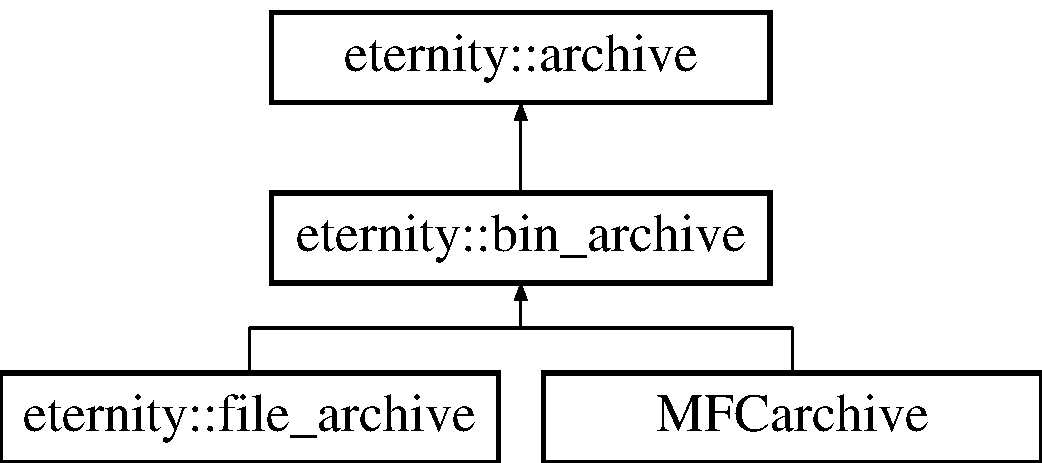
\includegraphics[height=3.000000cm]{classeternity_1_1bin__archive}
\end{center}
\end{figure}
\subsection*{Public Member Functions}
\begin{DoxyCompactItemize}
\item 
virtual \hyperlink{classeternity_1_1bin__archive_a0cc44edd050d598ff4f617e445159386}{$\sim$bin\+\_\+archive} ()
\item 
virtual size\+\_\+t \hyperlink{classeternity_1_1bin__archive_acbe041b0815f2721ee18ad042557b14e}{write} (const void $\ast$buffer, size\+\_\+t size, size\+\_\+t count)=0
\begin{DoxyCompactList}\small\item\em write a buffer of a certain legnth n time in the archive \end{DoxyCompactList}\item 
virtual size\+\_\+t \hyperlink{classeternity_1_1bin__archive_a5d67b032541f5a1e104d2fcd0eaa7a55}{read} (void $\ast$buffer, size\+\_\+t size, size\+\_\+t count)=0
\begin{DoxyCompactList}\small\item\em read a buffer of a certain legnth n time in the archive \end{DoxyCompactList}\item 
{\footnotesize template$<$class T $>$ }\\\hyperlink{classeternity_1_1bin__archive}{bin\+\_\+archive} \& \hyperlink{classeternity_1_1bin__archive_a451f9bd713b83922890014af88d386e6}{operator$<$$<$} (T \&ogg)
\item 
{\footnotesize template$<$class T $>$ }\\\hyperlink{classeternity_1_1bin__archive}{bin\+\_\+archive} \& \hyperlink{classeternity_1_1bin__archive_a8c431d394555d953019fe1f35ca77ffd}{operator$>$$>$} (T \&ogg)
\item 
\hyperlink{classeternity_1_1bin__archive}{bin\+\_\+archive} \& \hyperlink{classeternity_1_1bin__archive_a5cc61f7f70b1d809fbece79ccb9ecb26}{operator$<$$<$} (std\+::string \&str)
\begin{DoxyCompactList}\small\item\em Put a string in the archive. \end{DoxyCompactList}\item 
\hyperlink{classeternity_1_1bin__archive}{bin\+\_\+archive} \& \hyperlink{classeternity_1_1bin__archive_a4cbbd8dff6b78cf3868a49b30261dd26}{operator$>$$>$} (std\+::string \&str)
\begin{DoxyCompactList}\small\item\em Extract a string from the archive. \end{DoxyCompactList}\item 
{\footnotesize template$<$class t $>$ }\\t $\ast$ \hyperlink{classeternity_1_1bin__archive_a4c9b0ab9146c3a9ccaa5ec745299b282}{get\+\_\+object} (t $\ast$$\ast$pp\+Obj)
\begin{DoxyCompactList}\small\item\em Extract an object pointer from the archive. \end{DoxyCompactList}\item 
{\footnotesize template$<$class t $>$ }\\t $\ast$ \hyperlink{classeternity_1_1bin__archive_ab93c74313a8c6afdc65d4f2f2860502c}{put\+\_\+object} (t $\ast$p\+Obj)
\begin{DoxyCompactList}\small\item\em Put an object pointer in the archive. \end{DoxyCompactList}\end{DoxyCompactItemize}
\subsection*{Additional Inherited Members}


\subsection{Detailed Description}
Bin(ary)archive realize the persistence by serialization using a stream archive where to store in sequence all data in binary format. 

Definition at line 97 of file persist.\+hpp.



\subsection{Constructor \& Destructor Documentation}
\mbox{\Hypertarget{classeternity_1_1bin__archive_a0cc44edd050d598ff4f617e445159386}\label{classeternity_1_1bin__archive_a0cc44edd050d598ff4f617e445159386}} 
\index{eternity\+::bin\+\_\+archive@{eternity\+::bin\+\_\+archive}!````~bin\+\_\+archive@{$\sim$bin\+\_\+archive}}
\index{````~bin\+\_\+archive@{$\sim$bin\+\_\+archive}!eternity\+::bin\+\_\+archive@{eternity\+::bin\+\_\+archive}}
\subsubsection{\texorpdfstring{$\sim$bin\+\_\+archive()}{~bin\_archive()}}
{\footnotesize\ttfamily virtual eternity\+::bin\+\_\+archive\+::$\sim$bin\+\_\+archive (\begin{DoxyParamCaption}{ }\end{DoxyParamCaption})\hspace{0.3cm}{\ttfamily [inline]}, {\ttfamily [virtual]}}



Definition at line 100 of file persist.\+hpp.



\subsection{Member Function Documentation}
\mbox{\Hypertarget{classeternity_1_1bin__archive_a4c9b0ab9146c3a9ccaa5ec745299b282}\label{classeternity_1_1bin__archive_a4c9b0ab9146c3a9ccaa5ec745299b282}} 
\index{eternity\+::bin\+\_\+archive@{eternity\+::bin\+\_\+archive}!get\+\_\+object@{get\+\_\+object}}
\index{get\+\_\+object@{get\+\_\+object}!eternity\+::bin\+\_\+archive@{eternity\+::bin\+\_\+archive}}
\subsubsection{\texorpdfstring{get\+\_\+object()}{get\_object()}}
{\footnotesize\ttfamily template$<$class t $>$ \\
t$\ast$ eternity\+::bin\+\_\+archive\+::get\+\_\+object (\begin{DoxyParamCaption}\item[{t $\ast$$\ast$}]{pp\+Obj }\end{DoxyParamCaption})\hspace{0.3cm}{\ttfamily [inline]}}



Extract an object pointer from the archive. 



Definition at line 138 of file persist.\+hpp.

\mbox{\Hypertarget{classeternity_1_1bin__archive_a451f9bd713b83922890014af88d386e6}\label{classeternity_1_1bin__archive_a451f9bd713b83922890014af88d386e6}} 
\index{eternity\+::bin\+\_\+archive@{eternity\+::bin\+\_\+archive}!operator$<$$<$@{operator$<$$<$}}
\index{operator$<$$<$@{operator$<$$<$}!eternity\+::bin\+\_\+archive@{eternity\+::bin\+\_\+archive}}
\subsubsection{\texorpdfstring{operator$<$$<$()}{operator<<()}\hspace{0.1cm}{\footnotesize\ttfamily [1/2]}}
{\footnotesize\ttfamily template$<$class T $>$ \\
\hyperlink{classeternity_1_1bin__archive}{bin\+\_\+archive}\& eternity\+::bin\+\_\+archive\+::operator$<$$<$ (\begin{DoxyParamCaption}\item[{T \&}]{ogg }\end{DoxyParamCaption})\hspace{0.3cm}{\ttfamily [inline]}}

Template operator to put any type ( except string) of proprieties in the archive. 

Definition at line 112 of file persist.\+hpp.

\mbox{\Hypertarget{classeternity_1_1bin__archive_a5cc61f7f70b1d809fbece79ccb9ecb26}\label{classeternity_1_1bin__archive_a5cc61f7f70b1d809fbece79ccb9ecb26}} 
\index{eternity\+::bin\+\_\+archive@{eternity\+::bin\+\_\+archive}!operator$<$$<$@{operator$<$$<$}}
\index{operator$<$$<$@{operator$<$$<$}!eternity\+::bin\+\_\+archive@{eternity\+::bin\+\_\+archive}}
\subsubsection{\texorpdfstring{operator$<$$<$()}{operator<<()}\hspace{0.1cm}{\footnotesize\ttfamily [2/2]}}
{\footnotesize\ttfamily \hyperlink{classeternity_1_1bin__archive}{bin\+\_\+archive} \& eternity\+::bin\+\_\+archive\+::operator$<$$<$ (\begin{DoxyParamCaption}\item[{std\+::string \&}]{str }\end{DoxyParamCaption})}



Put a string in the archive. 



Definition at line 41 of file persist.\+cpp.

\mbox{\Hypertarget{classeternity_1_1bin__archive_a8c431d394555d953019fe1f35ca77ffd}\label{classeternity_1_1bin__archive_a8c431d394555d953019fe1f35ca77ffd}} 
\index{eternity\+::bin\+\_\+archive@{eternity\+::bin\+\_\+archive}!operator$>$$>$@{operator$>$$>$}}
\index{operator$>$$>$@{operator$>$$>$}!eternity\+::bin\+\_\+archive@{eternity\+::bin\+\_\+archive}}
\subsubsection{\texorpdfstring{operator$>$$>$()}{operator>>()}\hspace{0.1cm}{\footnotesize\ttfamily [1/2]}}
{\footnotesize\ttfamily template$<$class T $>$ \\
\hyperlink{classeternity_1_1bin__archive}{bin\+\_\+archive}\& eternity\+::bin\+\_\+archive\+::operator$>$$>$ (\begin{DoxyParamCaption}\item[{T \&}]{ogg }\end{DoxyParamCaption})\hspace{0.3cm}{\ttfamily [inline]}}

Template operator to extract any type ( except string) of proprieties from the archive. 

Definition at line 122 of file persist.\+hpp.

\mbox{\Hypertarget{classeternity_1_1bin__archive_a4cbbd8dff6b78cf3868a49b30261dd26}\label{classeternity_1_1bin__archive_a4cbbd8dff6b78cf3868a49b30261dd26}} 
\index{eternity\+::bin\+\_\+archive@{eternity\+::bin\+\_\+archive}!operator$>$$>$@{operator$>$$>$}}
\index{operator$>$$>$@{operator$>$$>$}!eternity\+::bin\+\_\+archive@{eternity\+::bin\+\_\+archive}}
\subsubsection{\texorpdfstring{operator$>$$>$()}{operator>>()}\hspace{0.1cm}{\footnotesize\ttfamily [2/2]}}
{\footnotesize\ttfamily \hyperlink{classeternity_1_1bin__archive}{bin\+\_\+archive} \& eternity\+::bin\+\_\+archive\+::operator$>$$>$ (\begin{DoxyParamCaption}\item[{std\+::string \&}]{str }\end{DoxyParamCaption})}



Extract a string from the archive. 



Definition at line 58 of file persist.\+cpp.

\mbox{\Hypertarget{classeternity_1_1bin__archive_ab93c74313a8c6afdc65d4f2f2860502c}\label{classeternity_1_1bin__archive_ab93c74313a8c6afdc65d4f2f2860502c}} 
\index{eternity\+::bin\+\_\+archive@{eternity\+::bin\+\_\+archive}!put\+\_\+object@{put\+\_\+object}}
\index{put\+\_\+object@{put\+\_\+object}!eternity\+::bin\+\_\+archive@{eternity\+::bin\+\_\+archive}}
\subsubsection{\texorpdfstring{put\+\_\+object()}{put\_object()}}
{\footnotesize\ttfamily template$<$class t $>$ \\
t$\ast$ eternity\+::bin\+\_\+archive\+::put\+\_\+object (\begin{DoxyParamCaption}\item[{t $\ast$}]{p\+Obj }\end{DoxyParamCaption})\hspace{0.3cm}{\ttfamily [inline]}}



Put an object pointer in the archive. 



Definition at line 168 of file persist.\+hpp.

\mbox{\Hypertarget{classeternity_1_1bin__archive_a5d67b032541f5a1e104d2fcd0eaa7a55}\label{classeternity_1_1bin__archive_a5d67b032541f5a1e104d2fcd0eaa7a55}} 
\index{eternity\+::bin\+\_\+archive@{eternity\+::bin\+\_\+archive}!read@{read}}
\index{read@{read}!eternity\+::bin\+\_\+archive@{eternity\+::bin\+\_\+archive}}
\subsubsection{\texorpdfstring{read()}{read()}}
{\footnotesize\ttfamily virtual size\+\_\+t eternity\+::bin\+\_\+archive\+::read (\begin{DoxyParamCaption}\item[{void $\ast$}]{buffer,  }\item[{size\+\_\+t}]{size,  }\item[{size\+\_\+t}]{count }\end{DoxyParamCaption})\hspace{0.3cm}{\ttfamily [pure virtual]}}



read a buffer of a certain legnth n time in the archive 



Implemented in \hyperlink{classeternity_1_1file__archive_a307b43ac9f06c7077ac0f7e48dc0d7ab}{eternity\+::file\+\_\+archive}, and \hyperlink{class_m_f_carchive_a175a083e8f81fe490714be920539f7b9}{M\+F\+Carchive}.

\mbox{\Hypertarget{classeternity_1_1bin__archive_acbe041b0815f2721ee18ad042557b14e}\label{classeternity_1_1bin__archive_acbe041b0815f2721ee18ad042557b14e}} 
\index{eternity\+::bin\+\_\+archive@{eternity\+::bin\+\_\+archive}!write@{write}}
\index{write@{write}!eternity\+::bin\+\_\+archive@{eternity\+::bin\+\_\+archive}}
\subsubsection{\texorpdfstring{write()}{write()}}
{\footnotesize\ttfamily virtual size\+\_\+t eternity\+::bin\+\_\+archive\+::write (\begin{DoxyParamCaption}\item[{const void $\ast$}]{buffer,  }\item[{size\+\_\+t}]{size,  }\item[{size\+\_\+t}]{count }\end{DoxyParamCaption})\hspace{0.3cm}{\ttfamily [pure virtual]}}



write a buffer of a certain legnth n time in the archive 



Implemented in \hyperlink{classeternity_1_1file__archive_a0eaf4b5937b3ff46df3627f64efc19e8}{eternity\+::file\+\_\+archive}, and \hyperlink{class_m_f_carchive_a8c5191701a84b9a4d2812887cfc28651}{M\+F\+Carchive}.



The documentation for this class was generated from the following files\+:\begin{DoxyCompactItemize}
\item 
/home/filip/\+Ph\+D/\+W\+D\+F\+Pipe\+\_\+test/p4\+T\+S\+A/include/eternity/\hyperlink{persist_8hpp}{persist.\+hpp}\item 
/home/filip/\+Ph\+D/\+W\+D\+F\+Pipe\+\_\+test/p4\+T\+S\+A/include/eternity/\hyperlink{persist_8cpp}{persist.\+cpp}\end{DoxyCompactItemize}

\hypertarget{classtsa_1_1_bisquare_window}{}\section{tsa\+:\+:Bisquare\+Window Class Reference}
\label{classtsa_1_1_bisquare_window}\index{tsa\+::\+Bisquare\+Window@{tsa\+::\+Bisquare\+Window}}


Bisquare windowing algorithm.  




{\ttfamily \#include $<$Bisquare\+Window.\+hpp$>$}

Inheritance diagram for tsa\+:\+:Bisquare\+Window\+:\begin{figure}[H]
\begin{center}
\leavevmode
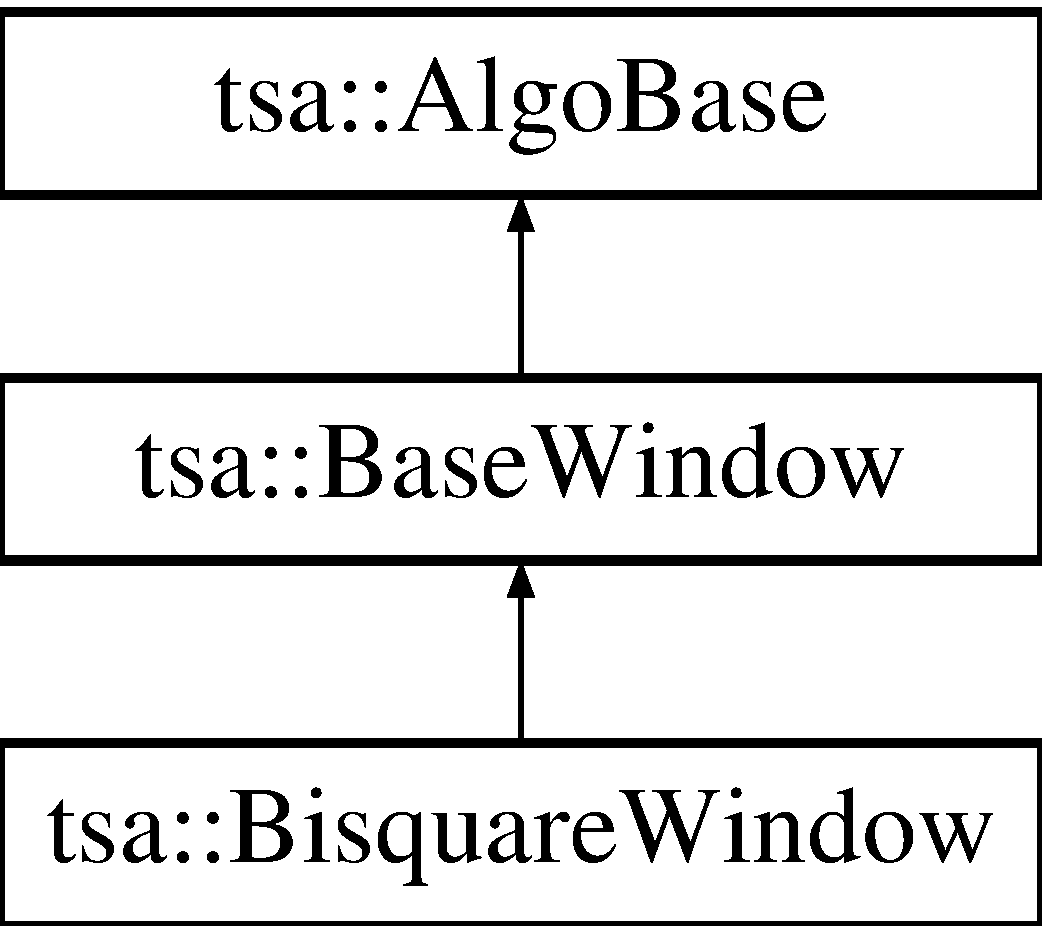
\includegraphics[height=3.000000cm]{classtsa_1_1_bisquare_window}
\end{center}
\end{figure}
\subsection*{Public Member Functions}
\begin{DoxyCompactItemize}
\item 
\hyperlink{classtsa_1_1_bisquare_window_a6e5d4dbf8578ed2e9b516d9410c91156}{Bisquare\+Window} (int size)
\item 
\hyperlink{classtsa_1_1_bisquare_window_a3a76063272e48da547740c73de3c938e}{Bisquare\+Window} (int size, const std\+::string \&)
\item 
virtual \hyperlink{classtsa_1_1_bisquare_window_a050ef95c31279607ac93d854cbcf0670}{$\sim$\+Bisquare\+Window} ()
\end{DoxyCompactItemize}
\begin{Indent}\textbf{ Operations}\par
\begin{DoxyCompactItemize}
\item 
void \hyperlink{classtsa_1_1_bisquare_window_a8ad862435b17d306997adbb8be9c9b4f}{operator()} (\hyperlink{namespacetsa_ac599574bcc094eda25613724b8f3ca9e}{Seq\+View\+Double} \&v1)
\item 
void \hyperlink{classtsa_1_1_bisquare_window_a18002b225ed630af739a983da72a4006}{operator()} (\hyperlink{namespacetsa_ac599574bcc094eda25613724b8f3ca9e}{Seq\+View\+Double} \&v1, \hyperlink{namespacetsa_ac599574bcc094eda25613724b8f3ca9e}{Seq\+View\+Double} \&v2)
\item 
void \hyperlink{classtsa_1_1_bisquare_window_a0970518373e007e0fdd95701ff744c6f}{Resize} (unsigned int size)
\end{DoxyCompactItemize}
\end{Indent}
\subsection*{Private Member Functions}
\begin{DoxyCompactItemize}
\item 
void \hyperlink{classtsa_1_1_bisquare_window_a62ab3bab83dd4dd77090c7c49be24acb}{Fill\+Window} ()
\end{DoxyCompactItemize}
\subsection*{Additional Inherited Members}


\subsection{Detailed Description}
Bisquare windowing algorithm. 

Definition at line 69 of file Bisquare\+Window.\+hpp.



\subsection{Constructor \& Destructor Documentation}
\mbox{\Hypertarget{classtsa_1_1_bisquare_window_a6e5d4dbf8578ed2e9b516d9410c91156}\label{classtsa_1_1_bisquare_window_a6e5d4dbf8578ed2e9b516d9410c91156}} 
\index{tsa\+::\+Bisquare\+Window@{tsa\+::\+Bisquare\+Window}!Bisquare\+Window@{Bisquare\+Window}}
\index{Bisquare\+Window@{Bisquare\+Window}!tsa\+::\+Bisquare\+Window@{tsa\+::\+Bisquare\+Window}}
\subsubsection{\texorpdfstring{Bisquare\+Window()}{BisquareWindow()}\hspace{0.1cm}{\footnotesize\ttfamily [1/2]}}
{\footnotesize\ttfamily tsa\+::\+Bisquare\+Window\+::\+Bisquare\+Window (\begin{DoxyParamCaption}\item[{int}]{size }\end{DoxyParamCaption})\hspace{0.3cm}{\ttfamily [inline]}}

Constructor


\begin{DoxyParams}{Parameters}
{\em size} & the size of the window \\
\hline
{\em cached} & true if the window must be preevaluated in a buffer \\
\hline
\end{DoxyParams}


Definition at line 78 of file Bisquare\+Window.\+hpp.

\mbox{\Hypertarget{classtsa_1_1_bisquare_window_a3a76063272e48da547740c73de3c938e}\label{classtsa_1_1_bisquare_window_a3a76063272e48da547740c73de3c938e}} 
\index{tsa\+::\+Bisquare\+Window@{tsa\+::\+Bisquare\+Window}!Bisquare\+Window@{Bisquare\+Window}}
\index{Bisquare\+Window@{Bisquare\+Window}!tsa\+::\+Bisquare\+Window@{tsa\+::\+Bisquare\+Window}}
\subsubsection{\texorpdfstring{Bisquare\+Window()}{BisquareWindow()}\hspace{0.1cm}{\footnotesize\ttfamily [2/2]}}
{\footnotesize\ttfamily tsa\+::\+Bisquare\+Window\+::\+Bisquare\+Window (\begin{DoxyParamCaption}\item[{int}]{size,  }\item[{const std\+::string \&}]{ }\end{DoxyParamCaption})\hspace{0.3cm}{\ttfamily [inline]}}



Definition at line 84 of file Bisquare\+Window.\+hpp.

\mbox{\Hypertarget{classtsa_1_1_bisquare_window_a050ef95c31279607ac93d854cbcf0670}\label{classtsa_1_1_bisquare_window_a050ef95c31279607ac93d854cbcf0670}} 
\index{tsa\+::\+Bisquare\+Window@{tsa\+::\+Bisquare\+Window}!````~Bisquare\+Window@{$\sim$\+Bisquare\+Window}}
\index{````~Bisquare\+Window@{$\sim$\+Bisquare\+Window}!tsa\+::\+Bisquare\+Window@{tsa\+::\+Bisquare\+Window}}
\subsubsection{\texorpdfstring{$\sim$\+Bisquare\+Window()}{~BisquareWindow()}}
{\footnotesize\ttfamily virtual tsa\+::\+Bisquare\+Window\+::$\sim$\+Bisquare\+Window (\begin{DoxyParamCaption}{ }\end{DoxyParamCaption})\hspace{0.3cm}{\ttfamily [inline]}, {\ttfamily [virtual]}}

Destructor 

Definition at line 93 of file Bisquare\+Window.\+hpp.



\subsection{Member Function Documentation}
\mbox{\Hypertarget{classtsa_1_1_bisquare_window_a62ab3bab83dd4dd77090c7c49be24acb}\label{classtsa_1_1_bisquare_window_a62ab3bab83dd4dd77090c7c49be24acb}} 
\index{tsa\+::\+Bisquare\+Window@{tsa\+::\+Bisquare\+Window}!Fill\+Window@{Fill\+Window}}
\index{Fill\+Window@{Fill\+Window}!tsa\+::\+Bisquare\+Window@{tsa\+::\+Bisquare\+Window}}
\subsubsection{\texorpdfstring{Fill\+Window()}{FillWindow()}}
{\footnotesize\ttfamily void tsa\+::\+Bisquare\+Window\+::\+Fill\+Window (\begin{DoxyParamCaption}{ }\end{DoxyParamCaption})\hspace{0.3cm}{\ttfamily [inline]}, {\ttfamily [private]}, {\ttfamily [virtual]}}

Initialize the window with the correct values, given its actual size. This is a pure virtual function, which is redefined by each window class. 

Reimplemented from \hyperlink{classtsa_1_1_base_window_aa74b29105d94caa521d308198e8e6643}{tsa\+::\+Base\+Window}.



Definition at line 196 of file Bisquare\+Window.\+hpp.

\mbox{\Hypertarget{classtsa_1_1_bisquare_window_a8ad862435b17d306997adbb8be9c9b4f}\label{classtsa_1_1_bisquare_window_a8ad862435b17d306997adbb8be9c9b4f}} 
\index{tsa\+::\+Bisquare\+Window@{tsa\+::\+Bisquare\+Window}!operator()@{operator()}}
\index{operator()@{operator()}!tsa\+::\+Bisquare\+Window@{tsa\+::\+Bisquare\+Window}}
\subsubsection{\texorpdfstring{operator()()}{operator()()}\hspace{0.1cm}{\footnotesize\ttfamily [1/2]}}
{\footnotesize\ttfamily void tsa\+::\+Bisquare\+Window\+::operator() (\begin{DoxyParamCaption}\item[{\hyperlink{namespacetsa_ac599574bcc094eda25613724b8f3ca9e}{Seq\+View\+Double} \&}]{v1 }\end{DoxyParamCaption})\hspace{0.3cm}{\ttfamily [inline]}, {\ttfamily [virtual]}}

Apply the window to a given time view.


\begin{DoxyParams}{Parameters}
{\em v1} & the time view \\
\hline
\end{DoxyParams}


Reimplemented from \hyperlink{classtsa_1_1_base_window_a05d9edb95dc01840a1b2df78dfa3a8c1}{tsa\+::\+Base\+Window}.



Definition at line 107 of file Bisquare\+Window.\+hpp.

\mbox{\Hypertarget{classtsa_1_1_bisquare_window_a18002b225ed630af739a983da72a4006}\label{classtsa_1_1_bisquare_window_a18002b225ed630af739a983da72a4006}} 
\index{tsa\+::\+Bisquare\+Window@{tsa\+::\+Bisquare\+Window}!operator()@{operator()}}
\index{operator()@{operator()}!tsa\+::\+Bisquare\+Window@{tsa\+::\+Bisquare\+Window}}
\subsubsection{\texorpdfstring{operator()()}{operator()()}\hspace{0.1cm}{\footnotesize\ttfamily [2/2]}}
{\footnotesize\ttfamily void tsa\+::\+Bisquare\+Window\+::operator() (\begin{DoxyParamCaption}\item[{\hyperlink{namespacetsa_ac599574bcc094eda25613724b8f3ca9e}{Seq\+View\+Double} \&}]{v1,  }\item[{\hyperlink{namespacetsa_ac599574bcc094eda25613724b8f3ca9e}{Seq\+View\+Double} \&}]{v2 }\end{DoxyParamCaption})\hspace{0.3cm}{\ttfamily [inline]}, {\ttfamily [virtual]}}

Apply a window to an input view and write the results on a output view.


\begin{DoxyParams}{Parameters}
{\em v1} & the input view \\
\hline
{\em v2} & the output view \\
\hline
\end{DoxyParams}


Reimplemented from \hyperlink{classtsa_1_1_base_window_afda50daa943527e09792b06e5ba69bcb}{tsa\+::\+Base\+Window}.



Definition at line 129 of file Bisquare\+Window.\+hpp.

\mbox{\Hypertarget{classtsa_1_1_bisquare_window_a0970518373e007e0fdd95701ff744c6f}\label{classtsa_1_1_bisquare_window_a0970518373e007e0fdd95701ff744c6f}} 
\index{tsa\+::\+Bisquare\+Window@{tsa\+::\+Bisquare\+Window}!Resize@{Resize}}
\index{Resize@{Resize}!tsa\+::\+Bisquare\+Window@{tsa\+::\+Bisquare\+Window}}
\subsubsection{\texorpdfstring{Resize()}{Resize()}}
{\footnotesize\ttfamily void tsa\+::\+Bisquare\+Window\+::\+Resize (\begin{DoxyParamCaption}\item[{unsigned int}]{size }\end{DoxyParamCaption})\hspace{0.3cm}{\ttfamily [inline]}, {\ttfamily [virtual]}}

Resize the window dimension.


\begin{DoxyParams}{Parameters}
{\em size} & new size for the window \\
\hline
\end{DoxyParams}


Reimplemented from \hyperlink{classtsa_1_1_base_window_a8a2a3425f2915762d50fa57dd0e04f22}{tsa\+::\+Base\+Window}.



Definition at line 158 of file Bisquare\+Window.\+hpp.



The documentation for this class was generated from the following file\+:\begin{DoxyCompactItemize}
\item 
/home/filip/\+Ph\+D/\+W\+D\+F\+Pipe\+\_\+test/p4\+T\+S\+A/include/\hyperlink{_bisquare_window_8hpp}{Bisquare\+Window.\+hpp}\end{DoxyCompactItemize}

\hypertarget{classtsa_1_1_b_l_interpolation}{}\section{tsa\+:\+:B\+L\+Interpolation Class Reference}
\label{classtsa_1_1_b_l_interpolation}\index{tsa\+::\+B\+L\+Interpolation@{tsa\+::\+B\+L\+Interpolation}}


Band limited interpolation.  




{\ttfamily \#include $<$B\+L\+Interpolation.\+hpp$>$}

Inheritance diagram for tsa\+:\+:B\+L\+Interpolation\+:\begin{figure}[H]
\begin{center}
\leavevmode
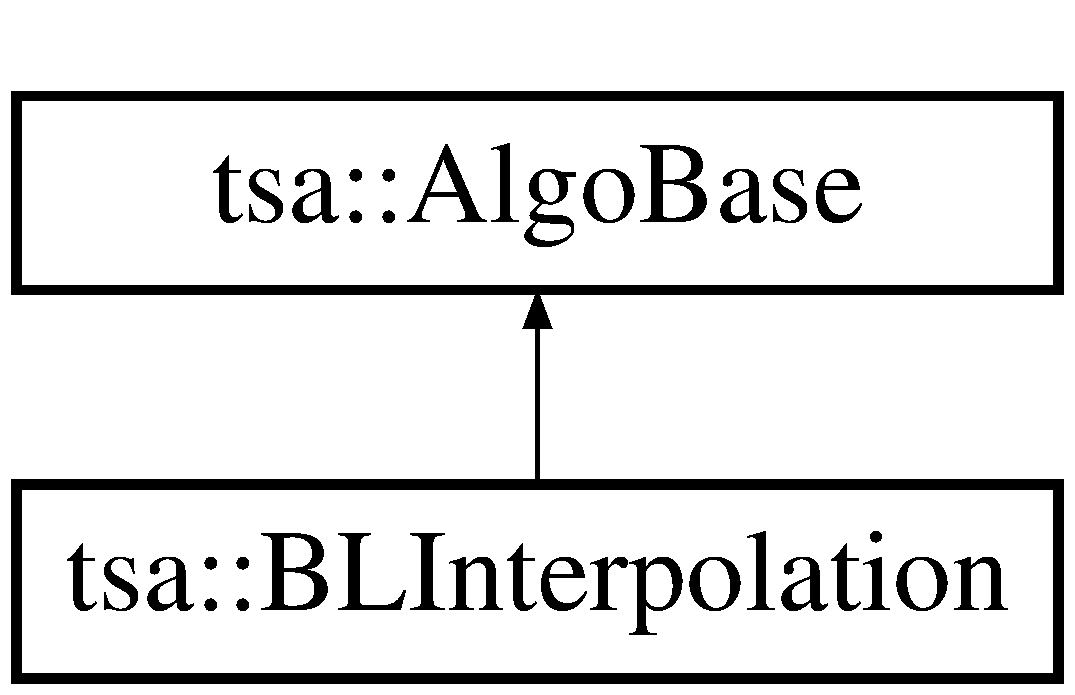
\includegraphics[height=2.000000cm]{classtsa_1_1_b_l_interpolation}
\end{center}
\end{figure}
\subsection*{Public Types}
\begin{DoxyCompactItemize}
\item 
enum \hyperlink{classtsa_1_1_b_l_interpolation_ae11719d30e353da11f076289b87c7b1d}{Normalization\+Type} \{ \hyperlink{classtsa_1_1_b_l_interpolation_ae11719d30e353da11f076289b87c7b1da2eb150e3b7e6ed1aff3dadd9dae02b5b}{N\+O\+Normalization}, 
\hyperlink{classtsa_1_1_b_l_interpolation_ae11719d30e353da11f076289b87c7b1da203bdef13ad529ea833b62c762c1a395}{D\+C\+Normalization}
 \}
\end{DoxyCompactItemize}
\subsection*{Public Member Functions}
\begin{DoxyCompactItemize}
\item 
\hyperlink{classtsa_1_1_b_l_interpolation_aef84f84620a59efee8d1e2bb1cffd46d}{B\+L\+Interpolation} (unsigned int channels, unsigned int outdata, unsigned int irate, unsigned int orate, unsigned int order, double alpha=1.\+0, enum \hyperlink{classtsa_1_1_b_l_interpolation_ae11719d30e353da11f076289b87c7b1d}{Normalization\+Type} nt=\hyperlink{classtsa_1_1_b_l_interpolation_ae11719d30e353da11f076289b87c7b1da2eb150e3b7e6ed1aff3dadd9dae02b5b}{N\+O\+Normalization})
\item 
\hyperlink{classtsa_1_1_b_l_interpolation_ace4ab80e2c9f5147685bd22d5ee5841e}{B\+L\+Interpolation} (const \hyperlink{classtsa_1_1_b_l_interpolation}{B\+L\+Interpolation} \&from)
\item 
\hyperlink{classtsa_1_1_b_l_interpolation_a67cd882b93c7643cd0fdce08b7fa876f}{$\sim$\+B\+L\+Interpolation} ()
\item 
\hyperlink{classtsa_1_1_b_l_interpolation}{B\+L\+Interpolation} \& \hyperlink{classtsa_1_1_b_l_interpolation_a71b2bc1e0a68abe528d5c753b4a5c1c1}{operator=} (const \hyperlink{classtsa_1_1_b_l_interpolation}{B\+L\+Interpolation} \&from)
\end{DoxyCompactItemize}
\begin{Indent}\textbf{ User interface}\par
\begin{DoxyCompactItemize}
\item 
\hyperlink{classtsa_1_1_b_l_interpolation}{B\+L\+Interpolation} \& \hyperlink{classtsa_1_1_b_l_interpolation_ad4ce3e5cb5bc89e8de11a0dc1d54121e}{Input} (\hyperlink{namespacetsa_ac599574bcc094eda25613724b8f3ca9e}{Seq\+View\+Double} \&indata)
\item 
\hyperlink{classtsa_1_1_b_l_interpolation}{B\+L\+Interpolation} \& \hyperlink{classtsa_1_1_b_l_interpolation_aa67c8de249d447dea6bb6b9d353139bc}{Output} (\hyperlink{namespacetsa_ac599574bcc094eda25613724b8f3ca9e}{Seq\+View\+Double} \&outdata)
\end{DoxyCompactItemize}
\end{Indent}
\begin{Indent}\textbf{ Getters}\par
\begin{DoxyCompactItemize}
\item 
long int \hyperlink{classtsa_1_1_b_l_interpolation_a10f95a5ac0e7cc6981d30ed420404a3d}{Get\+Data\+Available} ()
\item 
unsigned int \hyperlink{classtsa_1_1_b_l_interpolation_a30ed4268c0691edf852ddb3c2ce541c7}{Get\+Data} (\hyperlink{namespacetsa_ad260cd21c1891c4ed391fe788569aba4}{Dmatrix} \&outdata)
\item 
double \hyperlink{classtsa_1_1_b_l_interpolation_a4fa7c4bfb9e12a3eb6767fc6b128093c}{Get\+Start\+Time} ()
\end{DoxyCompactItemize}
\end{Indent}
\begin{Indent}\textbf{ Setters}\par
\begin{DoxyCompactItemize}
\item 
void \hyperlink{classtsa_1_1_b_l_interpolation_ac8a67161f8c0aeb39ced9d36664860ba}{Set\+Data} (\hyperlink{namespacetsa_ad260cd21c1891c4ed391fe788569aba4}{Dmatrix} \&indata, double scale)
\end{DoxyCompactItemize}
\end{Indent}
\subsection*{Private Member Functions}
\begin{DoxyCompactItemize}
\item 
void \hyperlink{classtsa_1_1_b_l_interpolation_aff26a1c884d2733cebf280a556987e51}{Init} ()
\item 
void \hyperlink{classtsa_1_1_b_l_interpolation_a7b429b2867b887e3fec9d44c584f026c}{N\+O\+Renormalization} ()
\item 
void \hyperlink{classtsa_1_1_b_l_interpolation_a5d7f3b437e0aa09df7831c2b72a39f62}{D\+C\+Renormalization} ()
\item 
double \hyperlink{classtsa_1_1_b_l_interpolation_a8eeac8a3a0439f46764cf1455bd2febe}{Kaiser} (double x)
\item 
void \hyperlink{classtsa_1_1_b_l_interpolation_a23d1958ad6c23572e21c39ad421bf2a2}{add\+\_\+back\+\_\+point} ()
\item 
void \hyperlink{classtsa_1_1_b_l_interpolation_ac9f1957097458403fd2919445d3323db}{del\+\_\+front\+\_\+point} (unsigned int n)
\item 
long int \hyperlink{classtsa_1_1_b_l_interpolation_adfb54e2b5bd52c05c3caaf062f97d9b6}{resampled\+\_\+available} ()
\end{DoxyCompactItemize}
\subsection*{Private Attributes}
\begin{DoxyCompactItemize}
\item 
unsigned int \hyperlink{classtsa_1_1_b_l_interpolation_a1299ee71922f13c989b9961a0adcd14f}{m\+Channels}
\item 
unsigned int \hyperlink{classtsa_1_1_b_l_interpolation_ab8ea8e129045096ccb53d1b5e6d27329}{m\+Out\+Data}
\item 
unsigned int \hyperlink{classtsa_1_1_b_l_interpolation_a3fc5200b462e9fbd87644f2d5bfa4381}{m\+Input\+Rate}
\item 
unsigned int \hyperlink{classtsa_1_1_b_l_interpolation_a4511cbb0d6e97a901e8d52cffad670a1}{m\+Output\+Rate}
\item 
unsigned int \hyperlink{classtsa_1_1_b_l_interpolation_aa8c5e5637c561ed9b3eabe6b8027e5da}{m\+Order}
\item 
double \hyperlink{classtsa_1_1_b_l_interpolation_a768c64c85e393f975e2caaaba7bc5f90}{m\+Alpha}
\item 
std\+::queue$<$ \hyperlink{namespacetsa_a8900fb03d849baf447a1a0efe2561fb2}{Dvector} $\ast$ $>$ \hyperlink{classtsa_1_1_b_l_interpolation_ab7b685a2b64f9139ca4ea3907f6b0a07}{m\+Repository}
\item 
std\+::deque$<$ \hyperlink{namespacetsa_a8900fb03d849baf447a1a0efe2561fb2}{Dvector} $\ast$ $>$ \hyperlink{classtsa_1_1_b_l_interpolation_ad40701a7e17ce4a2368605c0e77ec6a7}{m\+Buffer}
\item 
long int \hyperlink{classtsa_1_1_b_l_interpolation_a7e179ad859cffc61384efe0bc841255b}{m\+Buffer\+Base}
\item 
double \hyperlink{classtsa_1_1_b_l_interpolation_a21a038009c7323c00263367ca678f767}{m\+Rho}
\item 
\hyperlink{namespacetsa_a8900fb03d849baf447a1a0efe2561fb2}{Dvector} $\ast$ \hyperlink{classtsa_1_1_b_l_interpolation_ab0b2cee3d403a0ae8d3cc3d5c0618f02}{m\+Filter}
\item 
long int \hyperlink{classtsa_1_1_b_l_interpolation_ac7684f2b6ae85030eac7992412df45aa}{m\+Filter\+Center}
\item 
\hyperlink{namespacetsa_a8900fb03d849baf447a1a0efe2561fb2}{Dvector} \hyperlink{classtsa_1_1_b_l_interpolation_a5390ed81fda1345890543a95ab91a6e2}{m\+Normalization}
\item 
\hyperlink{classtsa_1_1_b_l_interpolation_ae11719d30e353da11f076289b87c7b1d}{Normalization\+Type} \hyperlink{classtsa_1_1_b_l_interpolation_aa41a64576f7c0df22870378780d8f73d}{m\+Normalization\+Type}
\item 
bool \hyperlink{classtsa_1_1_b_l_interpolation_adf29f91edc45fbbf8127732fa4b971f0}{m\+First\+Data}
\item 
double \hyperlink{classtsa_1_1_b_l_interpolation_afed34dd05a75cc0eb6ce313a584aa9ef}{m\+Start\+Time}
\item 
double \hyperlink{classtsa_1_1_b_l_interpolation_a76258e5da0c92a792af987a3f2cf972d}{m\+Sampling}
\end{DoxyCompactItemize}


\subsection{Detailed Description}
Band limited interpolation. 

Definition at line 74 of file B\+L\+Interpolation.\+hpp.



\subsection{Member Enumeration Documentation}
\mbox{\Hypertarget{classtsa_1_1_b_l_interpolation_ae11719d30e353da11f076289b87c7b1d}\label{classtsa_1_1_b_l_interpolation_ae11719d30e353da11f076289b87c7b1d}} 
\index{tsa\+::\+B\+L\+Interpolation@{tsa\+::\+B\+L\+Interpolation}!Normalization\+Type@{Normalization\+Type}}
\index{Normalization\+Type@{Normalization\+Type}!tsa\+::\+B\+L\+Interpolation@{tsa\+::\+B\+L\+Interpolation}}
\subsubsection{\texorpdfstring{Normalization\+Type}{NormalizationType}}
{\footnotesize\ttfamily enum \hyperlink{classtsa_1_1_b_l_interpolation_ae11719d30e353da11f076289b87c7b1d}{tsa\+::\+B\+L\+Interpolation\+::\+Normalization\+Type}}

\begin{DoxyEnumFields}{Enumerator}
\raisebox{\heightof{T}}[0pt][0pt]{\index{N\+O\+Normalization@{N\+O\+Normalization}!tsa\+::\+B\+L\+Interpolation@{tsa\+::\+B\+L\+Interpolation}}\index{tsa\+::\+B\+L\+Interpolation@{tsa\+::\+B\+L\+Interpolation}!N\+O\+Normalization@{N\+O\+Normalization}}}\mbox{\Hypertarget{classtsa_1_1_b_l_interpolation_ae11719d30e353da11f076289b87c7b1da2eb150e3b7e6ed1aff3dadd9dae02b5b}\label{classtsa_1_1_b_l_interpolation_ae11719d30e353da11f076289b87c7b1da2eb150e3b7e6ed1aff3dadd9dae02b5b}} 
N\+O\+Normalization&\\
\hline

\raisebox{\heightof{T}}[0pt][0pt]{\index{D\+C\+Normalization@{D\+C\+Normalization}!tsa\+::\+B\+L\+Interpolation@{tsa\+::\+B\+L\+Interpolation}}\index{tsa\+::\+B\+L\+Interpolation@{tsa\+::\+B\+L\+Interpolation}!D\+C\+Normalization@{D\+C\+Normalization}}}\mbox{\Hypertarget{classtsa_1_1_b_l_interpolation_ae11719d30e353da11f076289b87c7b1da203bdef13ad529ea833b62c762c1a395}\label{classtsa_1_1_b_l_interpolation_ae11719d30e353da11f076289b87c7b1da203bdef13ad529ea833b62c762c1a395}} 
D\+C\+Normalization&\\
\hline

\end{DoxyEnumFields}


Definition at line 77 of file B\+L\+Interpolation.\+hpp.



\subsection{Constructor \& Destructor Documentation}
\mbox{\Hypertarget{classtsa_1_1_b_l_interpolation_aef84f84620a59efee8d1e2bb1cffd46d}\label{classtsa_1_1_b_l_interpolation_aef84f84620a59efee8d1e2bb1cffd46d}} 
\index{tsa\+::\+B\+L\+Interpolation@{tsa\+::\+B\+L\+Interpolation}!B\+L\+Interpolation@{B\+L\+Interpolation}}
\index{B\+L\+Interpolation@{B\+L\+Interpolation}!tsa\+::\+B\+L\+Interpolation@{tsa\+::\+B\+L\+Interpolation}}
\subsubsection{\texorpdfstring{B\+L\+Interpolation()}{BLInterpolation()}\hspace{0.1cm}{\footnotesize\ttfamily [1/2]}}
{\footnotesize\ttfamily tsa\+::\+B\+L\+Interpolation\+::\+B\+L\+Interpolation (\begin{DoxyParamCaption}\item[{unsigned int}]{channels,  }\item[{unsigned int}]{outdata,  }\item[{unsigned int}]{irate,  }\item[{unsigned int}]{orate,  }\item[{unsigned int}]{order,  }\item[{double}]{alpha = {\ttfamily 1.0},  }\item[{enum \hyperlink{classtsa_1_1_b_l_interpolation_ae11719d30e353da11f076289b87c7b1d}{Normalization\+Type}}]{nt = {\ttfamily \hyperlink{classtsa_1_1_b_l_interpolation_ae11719d30e353da11f076289b87c7b1da2eb150e3b7e6ed1aff3dadd9dae02b5b}{N\+O\+Normalization}} }\end{DoxyParamCaption})}

Constructor.


\begin{DoxyParams}{Parameters}
{\em channels} & number of channels \\
\hline
{\em outdata} & number of resampled data returned at each call \\
\hline
{\em irate} & input rate \\
\hline
{\em orate} & output rate \\
\hline
{\em order} & order of filter \\
\hline
{\em alpha} & window parameter \\
\hline
\end{DoxyParams}


Definition at line 5 of file B\+L\+Interpolation.\+cpp.

\mbox{\Hypertarget{classtsa_1_1_b_l_interpolation_ace4ab80e2c9f5147685bd22d5ee5841e}\label{classtsa_1_1_b_l_interpolation_ace4ab80e2c9f5147685bd22d5ee5841e}} 
\index{tsa\+::\+B\+L\+Interpolation@{tsa\+::\+B\+L\+Interpolation}!B\+L\+Interpolation@{B\+L\+Interpolation}}
\index{B\+L\+Interpolation@{B\+L\+Interpolation}!tsa\+::\+B\+L\+Interpolation@{tsa\+::\+B\+L\+Interpolation}}
\subsubsection{\texorpdfstring{B\+L\+Interpolation()}{BLInterpolation()}\hspace{0.1cm}{\footnotesize\ttfamily [2/2]}}
{\footnotesize\ttfamily tsa\+::\+B\+L\+Interpolation\+::\+B\+L\+Interpolation (\begin{DoxyParamCaption}\item[{const \hyperlink{classtsa_1_1_b_l_interpolation}{B\+L\+Interpolation} \&}]{from }\end{DoxyParamCaption})}

Copy constructor


\begin{DoxyParams}{Parameters}
{\em from} & The instance that must be copied \\
\hline
\end{DoxyParams}


Definition at line 24 of file B\+L\+Interpolation.\+cpp.

\mbox{\Hypertarget{classtsa_1_1_b_l_interpolation_a67cd882b93c7643cd0fdce08b7fa876f}\label{classtsa_1_1_b_l_interpolation_a67cd882b93c7643cd0fdce08b7fa876f}} 
\index{tsa\+::\+B\+L\+Interpolation@{tsa\+::\+B\+L\+Interpolation}!````~B\+L\+Interpolation@{$\sim$\+B\+L\+Interpolation}}
\index{````~B\+L\+Interpolation@{$\sim$\+B\+L\+Interpolation}!tsa\+::\+B\+L\+Interpolation@{tsa\+::\+B\+L\+Interpolation}}
\subsubsection{\texorpdfstring{$\sim$\+B\+L\+Interpolation()}{~BLInterpolation()}}
{\footnotesize\ttfamily tsa\+::\+B\+L\+Interpolation\+::$\sim$\+B\+L\+Interpolation (\begin{DoxyParamCaption}{ }\end{DoxyParamCaption})}

Destructor 

Definition at line 36 of file B\+L\+Interpolation.\+cpp.



\subsection{Member Function Documentation}
\mbox{\Hypertarget{classtsa_1_1_b_l_interpolation_a23d1958ad6c23572e21c39ad421bf2a2}\label{classtsa_1_1_b_l_interpolation_a23d1958ad6c23572e21c39ad421bf2a2}} 
\index{tsa\+::\+B\+L\+Interpolation@{tsa\+::\+B\+L\+Interpolation}!add\+\_\+back\+\_\+point@{add\+\_\+back\+\_\+point}}
\index{add\+\_\+back\+\_\+point@{add\+\_\+back\+\_\+point}!tsa\+::\+B\+L\+Interpolation@{tsa\+::\+B\+L\+Interpolation}}
\subsubsection{\texorpdfstring{add\+\_\+back\+\_\+point()}{add\_back\_point()}}
{\footnotesize\ttfamily void tsa\+::\+B\+L\+Interpolation\+::add\+\_\+back\+\_\+point (\begin{DoxyParamCaption}{ }\end{DoxyParamCaption})\hspace{0.3cm}{\ttfamily [private]}}

Add a new data point to the buffer. If possible this is taken from the repository, allocated otherwise. 

Definition at line 240 of file B\+L\+Interpolation.\+cpp.

\mbox{\Hypertarget{classtsa_1_1_b_l_interpolation_a5d7f3b437e0aa09df7831c2b72a39f62}\label{classtsa_1_1_b_l_interpolation_a5d7f3b437e0aa09df7831c2b72a39f62}} 
\index{tsa\+::\+B\+L\+Interpolation@{tsa\+::\+B\+L\+Interpolation}!D\+C\+Renormalization@{D\+C\+Renormalization}}
\index{D\+C\+Renormalization@{D\+C\+Renormalization}!tsa\+::\+B\+L\+Interpolation@{tsa\+::\+B\+L\+Interpolation}}
\subsubsection{\texorpdfstring{D\+C\+Renormalization()}{DCRenormalization()}}
{\footnotesize\ttfamily void tsa\+::\+B\+L\+Interpolation\+::\+D\+C\+Renormalization (\begin{DoxyParamCaption}{ }\end{DoxyParamCaption})\hspace{0.3cm}{\ttfamily [private]}}



Definition at line 276 of file B\+L\+Interpolation.\+cpp.

\mbox{\Hypertarget{classtsa_1_1_b_l_interpolation_ac9f1957097458403fd2919445d3323db}\label{classtsa_1_1_b_l_interpolation_ac9f1957097458403fd2919445d3323db}} 
\index{tsa\+::\+B\+L\+Interpolation@{tsa\+::\+B\+L\+Interpolation}!del\+\_\+front\+\_\+point@{del\+\_\+front\+\_\+point}}
\index{del\+\_\+front\+\_\+point@{del\+\_\+front\+\_\+point}!tsa\+::\+B\+L\+Interpolation@{tsa\+::\+B\+L\+Interpolation}}
\subsubsection{\texorpdfstring{del\+\_\+front\+\_\+point()}{del\_front\_point()}}
{\footnotesize\ttfamily void tsa\+::\+B\+L\+Interpolation\+::del\+\_\+front\+\_\+point (\begin{DoxyParamCaption}\item[{unsigned int}]{n }\end{DoxyParamCaption})\hspace{0.3cm}{\ttfamily [private]}}

Delete some points from the buffer (the oldest ones) and increment the start of the buffer position m\+Buffer


\begin{DoxyParams}{Parameters}
{\em n} & number of points to delete from the buffer \\
\hline
\end{DoxyParams}


Definition at line 249 of file B\+L\+Interpolation.\+cpp.

\mbox{\Hypertarget{classtsa_1_1_b_l_interpolation_a30ed4268c0691edf852ddb3c2ce541c7}\label{classtsa_1_1_b_l_interpolation_a30ed4268c0691edf852ddb3c2ce541c7}} 
\index{tsa\+::\+B\+L\+Interpolation@{tsa\+::\+B\+L\+Interpolation}!Get\+Data@{Get\+Data}}
\index{Get\+Data@{Get\+Data}!tsa\+::\+B\+L\+Interpolation@{tsa\+::\+B\+L\+Interpolation}}
\subsubsection{\texorpdfstring{Get\+Data()}{GetData()}}
{\footnotesize\ttfamily unsigned int tsa\+::\+B\+L\+Interpolation\+::\+Get\+Data (\begin{DoxyParamCaption}\item[{\hyperlink{namespacetsa_ad260cd21c1891c4ed391fe788569aba4}{Dmatrix} \&}]{outdata }\end{DoxyParamCaption})}

Get resampled data


\begin{DoxyParams}{Parameters}
{\em outdata} & a matrix which will be filled with resampled data\\
\hline
\end{DoxyParams}
\begin{DoxyReturn}{Returns}
the number of resampled data returned 
\end{DoxyReturn}


Definition at line 109 of file B\+L\+Interpolation.\+cpp.

\mbox{\Hypertarget{classtsa_1_1_b_l_interpolation_a10f95a5ac0e7cc6981d30ed420404a3d}\label{classtsa_1_1_b_l_interpolation_a10f95a5ac0e7cc6981d30ed420404a3d}} 
\index{tsa\+::\+B\+L\+Interpolation@{tsa\+::\+B\+L\+Interpolation}!Get\+Data\+Available@{Get\+Data\+Available}}
\index{Get\+Data\+Available@{Get\+Data\+Available}!tsa\+::\+B\+L\+Interpolation@{tsa\+::\+B\+L\+Interpolation}}
\subsubsection{\texorpdfstring{Get\+Data\+Available()}{GetDataAvailable()}}
{\footnotesize\ttfamily long int tsa\+::\+B\+L\+Interpolation\+::\+Get\+Data\+Available (\begin{DoxyParamCaption}{ }\end{DoxyParamCaption})\hspace{0.3cm}{\ttfamily [inline]}}



Definition at line 178 of file B\+L\+Interpolation.\+hpp.

\mbox{\Hypertarget{classtsa_1_1_b_l_interpolation_a4fa7c4bfb9e12a3eb6767fc6b128093c}\label{classtsa_1_1_b_l_interpolation_a4fa7c4bfb9e12a3eb6767fc6b128093c}} 
\index{tsa\+::\+B\+L\+Interpolation@{tsa\+::\+B\+L\+Interpolation}!Get\+Start\+Time@{Get\+Start\+Time}}
\index{Get\+Start\+Time@{Get\+Start\+Time}!tsa\+::\+B\+L\+Interpolation@{tsa\+::\+B\+L\+Interpolation}}
\subsubsection{\texorpdfstring{Get\+Start\+Time()}{GetStartTime()}}
{\footnotesize\ttfamily double tsa\+::\+B\+L\+Interpolation\+::\+Get\+Start\+Time (\begin{DoxyParamCaption}{ }\end{DoxyParamCaption})}

Start time of the next sequence of resampled data.

\begin{DoxyReturn}{Returns}
the start time of the next sequence of resampled data 
\end{DoxyReturn}


Definition at line 105 of file B\+L\+Interpolation.\+cpp.

\mbox{\Hypertarget{classtsa_1_1_b_l_interpolation_aff26a1c884d2733cebf280a556987e51}\label{classtsa_1_1_b_l_interpolation_aff26a1c884d2733cebf280a556987e51}} 
\index{tsa\+::\+B\+L\+Interpolation@{tsa\+::\+B\+L\+Interpolation}!Init@{Init}}
\index{Init@{Init}!tsa\+::\+B\+L\+Interpolation@{tsa\+::\+B\+L\+Interpolation}}
\subsubsection{\texorpdfstring{Init()}{Init()}}
{\footnotesize\ttfamily void tsa\+::\+B\+L\+Interpolation\+::\+Init (\begin{DoxyParamCaption}{ }\end{DoxyParamCaption})\hspace{0.3cm}{\ttfamily [private]}}

Initialize internal structures 

Definition at line 187 of file B\+L\+Interpolation.\+cpp.

\mbox{\Hypertarget{classtsa_1_1_b_l_interpolation_ad4ce3e5cb5bc89e8de11a0dc1d54121e}\label{classtsa_1_1_b_l_interpolation_ad4ce3e5cb5bc89e8de11a0dc1d54121e}} 
\index{tsa\+::\+B\+L\+Interpolation@{tsa\+::\+B\+L\+Interpolation}!Input@{Input}}
\index{Input@{Input}!tsa\+::\+B\+L\+Interpolation@{tsa\+::\+B\+L\+Interpolation}}
\subsubsection{\texorpdfstring{Input()}{Input()}}
{\footnotesize\ttfamily \hyperlink{classtsa_1_1_b_l_interpolation}{B\+L\+Interpolation} \& tsa\+::\+B\+L\+Interpolation\+::\+Input (\begin{DoxyParamCaption}\item[{\hyperlink{namespacetsa_ac599574bcc094eda25613724b8f3ca9e}{Seq\+View\+Double} \&}]{indata }\end{DoxyParamCaption})}

Add data to be resampled. This method can be called repeatedly, each time with a different chunk of data. The chunks are considered as consecutive pieces of a continuous stream.


\begin{DoxyParams}{Parameters}
{\em indata} & view containing input data\\
\hline
\end{DoxyParams}
\begin{DoxyReturn}{Returns}
a reference to an instance of this class
\end{DoxyReturn}
\begin{DoxyPrecond}{Precondition}
the number of rows in indata must be equal to the number of channels 
\end{DoxyPrecond}


Definition at line 67 of file B\+L\+Interpolation.\+cpp.

\mbox{\Hypertarget{classtsa_1_1_b_l_interpolation_a8eeac8a3a0439f46764cf1455bd2febe}\label{classtsa_1_1_b_l_interpolation_a8eeac8a3a0439f46764cf1455bd2febe}} 
\index{tsa\+::\+B\+L\+Interpolation@{tsa\+::\+B\+L\+Interpolation}!Kaiser@{Kaiser}}
\index{Kaiser@{Kaiser}!tsa\+::\+B\+L\+Interpolation@{tsa\+::\+B\+L\+Interpolation}}
\subsubsection{\texorpdfstring{Kaiser()}{Kaiser()}}
{\footnotesize\ttfamily double tsa\+::\+B\+L\+Interpolation\+::\+Kaiser (\begin{DoxyParamCaption}\item[{double}]{x }\end{DoxyParamCaption})\hspace{0.3cm}{\ttfamily [private]}}

Kaiser window.


\begin{DoxyParams}{Parameters}
{\em x} & position in the window (between -\/1 and 1)\\
\hline
\end{DoxyParams}
\begin{DoxyReturn}{Returns}
the value of Kaiser window at index k 
\end{DoxyReturn}


Definition at line 235 of file B\+L\+Interpolation.\+cpp.

\mbox{\Hypertarget{classtsa_1_1_b_l_interpolation_a7b429b2867b887e3fec9d44c584f026c}\label{classtsa_1_1_b_l_interpolation_a7b429b2867b887e3fec9d44c584f026c}} 
\index{tsa\+::\+B\+L\+Interpolation@{tsa\+::\+B\+L\+Interpolation}!N\+O\+Renormalization@{N\+O\+Renormalization}}
\index{N\+O\+Renormalization@{N\+O\+Renormalization}!tsa\+::\+B\+L\+Interpolation@{tsa\+::\+B\+L\+Interpolation}}
\subsubsection{\texorpdfstring{N\+O\+Renormalization()}{NORenormalization()}}
{\footnotesize\ttfamily void tsa\+::\+B\+L\+Interpolation\+::\+N\+O\+Renormalization (\begin{DoxyParamCaption}{ }\end{DoxyParamCaption})\hspace{0.3cm}{\ttfamily [private]}}



Definition at line 267 of file B\+L\+Interpolation.\+cpp.

\mbox{\Hypertarget{classtsa_1_1_b_l_interpolation_a71b2bc1e0a68abe528d5c753b4a5c1c1}\label{classtsa_1_1_b_l_interpolation_a71b2bc1e0a68abe528d5c753b4a5c1c1}} 
\index{tsa\+::\+B\+L\+Interpolation@{tsa\+::\+B\+L\+Interpolation}!operator=@{operator=}}
\index{operator=@{operator=}!tsa\+::\+B\+L\+Interpolation@{tsa\+::\+B\+L\+Interpolation}}
\subsubsection{\texorpdfstring{operator=()}{operator=()}}
{\footnotesize\ttfamily \hyperlink{classtsa_1_1_b_l_interpolation}{B\+L\+Interpolation} \& tsa\+::\+B\+L\+Interpolation\+::operator= (\begin{DoxyParamCaption}\item[{const \hyperlink{classtsa_1_1_b_l_interpolation}{B\+L\+Interpolation} \&}]{from }\end{DoxyParamCaption})}

Assignement operator


\begin{DoxyParams}{Parameters}
{\em from} & The instance to be assigned from\\
\hline
\end{DoxyParams}
\begin{DoxyReturn}{Returns}
a reference to a new object 
\end{DoxyReturn}


Definition at line 51 of file B\+L\+Interpolation.\+cpp.

\mbox{\Hypertarget{classtsa_1_1_b_l_interpolation_aa67c8de249d447dea6bb6b9d353139bc}\label{classtsa_1_1_b_l_interpolation_aa67c8de249d447dea6bb6b9d353139bc}} 
\index{tsa\+::\+B\+L\+Interpolation@{tsa\+::\+B\+L\+Interpolation}!Output@{Output}}
\index{Output@{Output}!tsa\+::\+B\+L\+Interpolation@{tsa\+::\+B\+L\+Interpolation}}
\subsubsection{\texorpdfstring{Output()}{Output()}}
{\footnotesize\ttfamily \hyperlink{classtsa_1_1_b_l_interpolation}{B\+L\+Interpolation} \& tsa\+::\+B\+L\+Interpolation\+::\+Output (\begin{DoxyParamCaption}\item[{\hyperlink{namespacetsa_ac599574bcc094eda25613724b8f3ca9e}{Seq\+View\+Double} \&}]{outdata }\end{DoxyParamCaption})}

Get resampled data. If there are enough resampled data available these are returned, otherwise an exception is raised.


\begin{DoxyParams}{Parameters}
{\em outdata} & view which will be filled with resampled data\\
\hline
\end{DoxyParams}
\begin{DoxyReturn}{Returns}
a reference to an instance of this class
\end{DoxyReturn}

\begin{DoxyExceptions}{Exceptions}
{\em \hyperlink{classtsa_1_1no__data__available}{no\+\_\+data\+\_\+available}} & there are not enough resampled data available\\
\hline
\end{DoxyExceptions}
\begin{DoxyPostcond}{Postcondition}
if no exception is raised outdata has a number of rows equal to the number of channels and a number of columns equal to the number of returned data 
\end{DoxyPostcond}


Definition at line 81 of file B\+L\+Interpolation.\+cpp.

\mbox{\Hypertarget{classtsa_1_1_b_l_interpolation_adfb54e2b5bd52c05c3caaf062f97d9b6}\label{classtsa_1_1_b_l_interpolation_adfb54e2b5bd52c05c3caaf062f97d9b6}} 
\index{tsa\+::\+B\+L\+Interpolation@{tsa\+::\+B\+L\+Interpolation}!resampled\+\_\+available@{resampled\+\_\+available}}
\index{resampled\+\_\+available@{resampled\+\_\+available}!tsa\+::\+B\+L\+Interpolation@{tsa\+::\+B\+L\+Interpolation}}
\subsubsection{\texorpdfstring{resampled\+\_\+available()}{resampled\_available()}}
{\footnotesize\ttfamily long int tsa\+::\+B\+L\+Interpolation\+::resampled\+\_\+available (\begin{DoxyParamCaption}{ }\end{DoxyParamCaption})\hspace{0.3cm}{\ttfamily [private]}}

This function returns the number of resampled data which are available at the current time.

\begin{DoxyReturn}{Returns}
resampled data available 
\end{DoxyReturn}


Definition at line 260 of file B\+L\+Interpolation.\+cpp.

\mbox{\Hypertarget{classtsa_1_1_b_l_interpolation_ac8a67161f8c0aeb39ced9d36664860ba}\label{classtsa_1_1_b_l_interpolation_ac8a67161f8c0aeb39ced9d36664860ba}} 
\index{tsa\+::\+B\+L\+Interpolation@{tsa\+::\+B\+L\+Interpolation}!Set\+Data@{Set\+Data}}
\index{Set\+Data@{Set\+Data}!tsa\+::\+B\+L\+Interpolation@{tsa\+::\+B\+L\+Interpolation}}
\subsubsection{\texorpdfstring{Set\+Data()}{SetData()}}
{\footnotesize\ttfamily void tsa\+::\+B\+L\+Interpolation\+::\+Set\+Data (\begin{DoxyParamCaption}\item[{\hyperlink{namespacetsa_ad260cd21c1891c4ed391fe788569aba4}{Dmatrix} \&}]{indata,  }\item[{double}]{scale }\end{DoxyParamCaption})}

Add data to be resampled


\begin{DoxyParams}{Parameters}
{\em indata} & a matrix which contains input data \\
\hline
{\em scale} & a scale parameter for input data \\
\hline
\end{DoxyParams}


Definition at line 169 of file B\+L\+Interpolation.\+cpp.



\subsection{Member Data Documentation}
\mbox{\Hypertarget{classtsa_1_1_b_l_interpolation_a768c64c85e393f975e2caaaba7bc5f90}\label{classtsa_1_1_b_l_interpolation_a768c64c85e393f975e2caaaba7bc5f90}} 
\index{tsa\+::\+B\+L\+Interpolation@{tsa\+::\+B\+L\+Interpolation}!m\+Alpha@{m\+Alpha}}
\index{m\+Alpha@{m\+Alpha}!tsa\+::\+B\+L\+Interpolation@{tsa\+::\+B\+L\+Interpolation}}
\subsubsection{\texorpdfstring{m\+Alpha}{mAlpha}}
{\footnotesize\ttfamily double tsa\+::\+B\+L\+Interpolation\+::m\+Alpha\hspace{0.3cm}{\ttfamily [private]}}

Parameter of the Kaiser window 

Definition at line 249 of file B\+L\+Interpolation.\+hpp.

\mbox{\Hypertarget{classtsa_1_1_b_l_interpolation_ad40701a7e17ce4a2368605c0e77ec6a7}\label{classtsa_1_1_b_l_interpolation_ad40701a7e17ce4a2368605c0e77ec6a7}} 
\index{tsa\+::\+B\+L\+Interpolation@{tsa\+::\+B\+L\+Interpolation}!m\+Buffer@{m\+Buffer}}
\index{m\+Buffer@{m\+Buffer}!tsa\+::\+B\+L\+Interpolation@{tsa\+::\+B\+L\+Interpolation}}
\subsubsection{\texorpdfstring{m\+Buffer}{mBuffer}}
{\footnotesize\ttfamily std\+::deque$<$\hyperlink{namespacetsa_a8900fb03d849baf447a1a0efe2561fb2}{Dvector}$\ast$$>$ tsa\+::\+B\+L\+Interpolation\+::m\+Buffer\hspace{0.3cm}{\ttfamily [private]}}

Buffer for incoming data points 

Definition at line 252 of file B\+L\+Interpolation.\+hpp.

\mbox{\Hypertarget{classtsa_1_1_b_l_interpolation_a7e179ad859cffc61384efe0bc841255b}\label{classtsa_1_1_b_l_interpolation_a7e179ad859cffc61384efe0bc841255b}} 
\index{tsa\+::\+B\+L\+Interpolation@{tsa\+::\+B\+L\+Interpolation}!m\+Buffer\+Base@{m\+Buffer\+Base}}
\index{m\+Buffer\+Base@{m\+Buffer\+Base}!tsa\+::\+B\+L\+Interpolation@{tsa\+::\+B\+L\+Interpolation}}
\subsubsection{\texorpdfstring{m\+Buffer\+Base}{mBufferBase}}
{\footnotesize\ttfamily long int tsa\+::\+B\+L\+Interpolation\+::m\+Buffer\+Base\hspace{0.3cm}{\ttfamily [private]}}

Start of the buffer, in ticks units 

Definition at line 253 of file B\+L\+Interpolation.\+hpp.

\mbox{\Hypertarget{classtsa_1_1_b_l_interpolation_a1299ee71922f13c989b9961a0adcd14f}\label{classtsa_1_1_b_l_interpolation_a1299ee71922f13c989b9961a0adcd14f}} 
\index{tsa\+::\+B\+L\+Interpolation@{tsa\+::\+B\+L\+Interpolation}!m\+Channels@{m\+Channels}}
\index{m\+Channels@{m\+Channels}!tsa\+::\+B\+L\+Interpolation@{tsa\+::\+B\+L\+Interpolation}}
\subsubsection{\texorpdfstring{m\+Channels}{mChannels}}
{\footnotesize\ttfamily unsigned int tsa\+::\+B\+L\+Interpolation\+::m\+Channels\hspace{0.3cm}{\ttfamily [private]}}

Number of channels to resample 

Definition at line 244 of file B\+L\+Interpolation.\+hpp.

\mbox{\Hypertarget{classtsa_1_1_b_l_interpolation_ab0b2cee3d403a0ae8d3cc3d5c0618f02}\label{classtsa_1_1_b_l_interpolation_ab0b2cee3d403a0ae8d3cc3d5c0618f02}} 
\index{tsa\+::\+B\+L\+Interpolation@{tsa\+::\+B\+L\+Interpolation}!m\+Filter@{m\+Filter}}
\index{m\+Filter@{m\+Filter}!tsa\+::\+B\+L\+Interpolation@{tsa\+::\+B\+L\+Interpolation}}
\subsubsection{\texorpdfstring{m\+Filter}{mFilter}}
{\footnotesize\ttfamily \hyperlink{namespacetsa_a8900fb03d849baf447a1a0efe2561fb2}{Dvector}$\ast$ tsa\+::\+B\+L\+Interpolation\+::m\+Filter\hspace{0.3cm}{\ttfamily [private]}}

Template for the filter 

Definition at line 257 of file B\+L\+Interpolation.\+hpp.

\mbox{\Hypertarget{classtsa_1_1_b_l_interpolation_ac7684f2b6ae85030eac7992412df45aa}\label{classtsa_1_1_b_l_interpolation_ac7684f2b6ae85030eac7992412df45aa}} 
\index{tsa\+::\+B\+L\+Interpolation@{tsa\+::\+B\+L\+Interpolation}!m\+Filter\+Center@{m\+Filter\+Center}}
\index{m\+Filter\+Center@{m\+Filter\+Center}!tsa\+::\+B\+L\+Interpolation@{tsa\+::\+B\+L\+Interpolation}}
\subsubsection{\texorpdfstring{m\+Filter\+Center}{mFilterCenter}}
{\footnotesize\ttfamily long int tsa\+::\+B\+L\+Interpolation\+::m\+Filter\+Center\hspace{0.3cm}{\ttfamily [private]}}

Center of the filter, in ticks units 

Definition at line 258 of file B\+L\+Interpolation.\+hpp.

\mbox{\Hypertarget{classtsa_1_1_b_l_interpolation_adf29f91edc45fbbf8127732fa4b971f0}\label{classtsa_1_1_b_l_interpolation_adf29f91edc45fbbf8127732fa4b971f0}} 
\index{tsa\+::\+B\+L\+Interpolation@{tsa\+::\+B\+L\+Interpolation}!m\+First\+Data@{m\+First\+Data}}
\index{m\+First\+Data@{m\+First\+Data}!tsa\+::\+B\+L\+Interpolation@{tsa\+::\+B\+L\+Interpolation}}
\subsubsection{\texorpdfstring{m\+First\+Data}{mFirstData}}
{\footnotesize\ttfamily bool tsa\+::\+B\+L\+Interpolation\+::m\+First\+Data\hspace{0.3cm}{\ttfamily [private]}}

Flag\+: is the actual view the first submitted? 

Definition at line 263 of file B\+L\+Interpolation.\+hpp.

\mbox{\Hypertarget{classtsa_1_1_b_l_interpolation_a3fc5200b462e9fbd87644f2d5bfa4381}\label{classtsa_1_1_b_l_interpolation_a3fc5200b462e9fbd87644f2d5bfa4381}} 
\index{tsa\+::\+B\+L\+Interpolation@{tsa\+::\+B\+L\+Interpolation}!m\+Input\+Rate@{m\+Input\+Rate}}
\index{m\+Input\+Rate@{m\+Input\+Rate}!tsa\+::\+B\+L\+Interpolation@{tsa\+::\+B\+L\+Interpolation}}
\subsubsection{\texorpdfstring{m\+Input\+Rate}{mInputRate}}
{\footnotesize\ttfamily unsigned int tsa\+::\+B\+L\+Interpolation\+::m\+Input\+Rate\hspace{0.3cm}{\ttfamily [private]}}

Input rate of data 

Definition at line 246 of file B\+L\+Interpolation.\+hpp.

\mbox{\Hypertarget{classtsa_1_1_b_l_interpolation_a5390ed81fda1345890543a95ab91a6e2}\label{classtsa_1_1_b_l_interpolation_a5390ed81fda1345890543a95ab91a6e2}} 
\index{tsa\+::\+B\+L\+Interpolation@{tsa\+::\+B\+L\+Interpolation}!m\+Normalization@{m\+Normalization}}
\index{m\+Normalization@{m\+Normalization}!tsa\+::\+B\+L\+Interpolation@{tsa\+::\+B\+L\+Interpolation}}
\subsubsection{\texorpdfstring{m\+Normalization}{mNormalization}}
{\footnotesize\ttfamily \hyperlink{namespacetsa_a8900fb03d849baf447a1a0efe2561fb2}{Dvector} tsa\+::\+B\+L\+Interpolation\+::m\+Normalization\hspace{0.3cm}{\ttfamily [private]}}



Definition at line 260 of file B\+L\+Interpolation.\+hpp.

\mbox{\Hypertarget{classtsa_1_1_b_l_interpolation_aa41a64576f7c0df22870378780d8f73d}\label{classtsa_1_1_b_l_interpolation_aa41a64576f7c0df22870378780d8f73d}} 
\index{tsa\+::\+B\+L\+Interpolation@{tsa\+::\+B\+L\+Interpolation}!m\+Normalization\+Type@{m\+Normalization\+Type}}
\index{m\+Normalization\+Type@{m\+Normalization\+Type}!tsa\+::\+B\+L\+Interpolation@{tsa\+::\+B\+L\+Interpolation}}
\subsubsection{\texorpdfstring{m\+Normalization\+Type}{mNormalizationType}}
{\footnotesize\ttfamily \hyperlink{classtsa_1_1_b_l_interpolation_ae11719d30e353da11f076289b87c7b1d}{Normalization\+Type} tsa\+::\+B\+L\+Interpolation\+::m\+Normalization\+Type\hspace{0.3cm}{\ttfamily [private]}}



Definition at line 261 of file B\+L\+Interpolation.\+hpp.

\mbox{\Hypertarget{classtsa_1_1_b_l_interpolation_aa8c5e5637c561ed9b3eabe6b8027e5da}\label{classtsa_1_1_b_l_interpolation_aa8c5e5637c561ed9b3eabe6b8027e5da}} 
\index{tsa\+::\+B\+L\+Interpolation@{tsa\+::\+B\+L\+Interpolation}!m\+Order@{m\+Order}}
\index{m\+Order@{m\+Order}!tsa\+::\+B\+L\+Interpolation@{tsa\+::\+B\+L\+Interpolation}}
\subsubsection{\texorpdfstring{m\+Order}{mOrder}}
{\footnotesize\ttfamily unsigned int tsa\+::\+B\+L\+Interpolation\+::m\+Order\hspace{0.3cm}{\ttfamily [private]}}

Order of the filter 

Definition at line 248 of file B\+L\+Interpolation.\+hpp.

\mbox{\Hypertarget{classtsa_1_1_b_l_interpolation_ab8ea8e129045096ccb53d1b5e6d27329}\label{classtsa_1_1_b_l_interpolation_ab8ea8e129045096ccb53d1b5e6d27329}} 
\index{tsa\+::\+B\+L\+Interpolation@{tsa\+::\+B\+L\+Interpolation}!m\+Out\+Data@{m\+Out\+Data}}
\index{m\+Out\+Data@{m\+Out\+Data}!tsa\+::\+B\+L\+Interpolation@{tsa\+::\+B\+L\+Interpolation}}
\subsubsection{\texorpdfstring{m\+Out\+Data}{mOutData}}
{\footnotesize\ttfamily unsigned int tsa\+::\+B\+L\+Interpolation\+::m\+Out\+Data\hspace{0.3cm}{\ttfamily [private]}}

Number of resampled data for channel that will be returned if possible at each call 

Definition at line 245 of file B\+L\+Interpolation.\+hpp.

\mbox{\Hypertarget{classtsa_1_1_b_l_interpolation_a4511cbb0d6e97a901e8d52cffad670a1}\label{classtsa_1_1_b_l_interpolation_a4511cbb0d6e97a901e8d52cffad670a1}} 
\index{tsa\+::\+B\+L\+Interpolation@{tsa\+::\+B\+L\+Interpolation}!m\+Output\+Rate@{m\+Output\+Rate}}
\index{m\+Output\+Rate@{m\+Output\+Rate}!tsa\+::\+B\+L\+Interpolation@{tsa\+::\+B\+L\+Interpolation}}
\subsubsection{\texorpdfstring{m\+Output\+Rate}{mOutputRate}}
{\footnotesize\ttfamily unsigned int tsa\+::\+B\+L\+Interpolation\+::m\+Output\+Rate\hspace{0.3cm}{\ttfamily [private]}}

Output rate of data 

Definition at line 247 of file B\+L\+Interpolation.\+hpp.

\mbox{\Hypertarget{classtsa_1_1_b_l_interpolation_ab7b685a2b64f9139ca4ea3907f6b0a07}\label{classtsa_1_1_b_l_interpolation_ab7b685a2b64f9139ca4ea3907f6b0a07}} 
\index{tsa\+::\+B\+L\+Interpolation@{tsa\+::\+B\+L\+Interpolation}!m\+Repository@{m\+Repository}}
\index{m\+Repository@{m\+Repository}!tsa\+::\+B\+L\+Interpolation@{tsa\+::\+B\+L\+Interpolation}}
\subsubsection{\texorpdfstring{m\+Repository}{mRepository}}
{\footnotesize\ttfamily std\+::queue$<$\hyperlink{namespacetsa_a8900fb03d849baf447a1a0efe2561fb2}{Dvector}$\ast$$>$ tsa\+::\+B\+L\+Interpolation\+::m\+Repository\hspace{0.3cm}{\ttfamily [private]}}

Repository for unused data points 

Definition at line 251 of file B\+L\+Interpolation.\+hpp.

\mbox{\Hypertarget{classtsa_1_1_b_l_interpolation_a21a038009c7323c00263367ca678f767}\label{classtsa_1_1_b_l_interpolation_a21a038009c7323c00263367ca678f767}} 
\index{tsa\+::\+B\+L\+Interpolation@{tsa\+::\+B\+L\+Interpolation}!m\+Rho@{m\+Rho}}
\index{m\+Rho@{m\+Rho}!tsa\+::\+B\+L\+Interpolation@{tsa\+::\+B\+L\+Interpolation}}
\subsubsection{\texorpdfstring{m\+Rho}{mRho}}
{\footnotesize\ttfamily double tsa\+::\+B\+L\+Interpolation\+::m\+Rho\hspace{0.3cm}{\ttfamily [private]}}

Normalization factor for upsampling/downsampling 

Definition at line 256 of file B\+L\+Interpolation.\+hpp.

\mbox{\Hypertarget{classtsa_1_1_b_l_interpolation_a76258e5da0c92a792af987a3f2cf972d}\label{classtsa_1_1_b_l_interpolation_a76258e5da0c92a792af987a3f2cf972d}} 
\index{tsa\+::\+B\+L\+Interpolation@{tsa\+::\+B\+L\+Interpolation}!m\+Sampling@{m\+Sampling}}
\index{m\+Sampling@{m\+Sampling}!tsa\+::\+B\+L\+Interpolation@{tsa\+::\+B\+L\+Interpolation}}
\subsubsection{\texorpdfstring{m\+Sampling}{mSampling}}
{\footnotesize\ttfamily double tsa\+::\+B\+L\+Interpolation\+::m\+Sampling\hspace{0.3cm}{\ttfamily [private]}}

Physical sampling rate 

Definition at line 265 of file B\+L\+Interpolation.\+hpp.

\mbox{\Hypertarget{classtsa_1_1_b_l_interpolation_afed34dd05a75cc0eb6ce313a584aa9ef}\label{classtsa_1_1_b_l_interpolation_afed34dd05a75cc0eb6ce313a584aa9ef}} 
\index{tsa\+::\+B\+L\+Interpolation@{tsa\+::\+B\+L\+Interpolation}!m\+Start\+Time@{m\+Start\+Time}}
\index{m\+Start\+Time@{m\+Start\+Time}!tsa\+::\+B\+L\+Interpolation@{tsa\+::\+B\+L\+Interpolation}}
\subsubsection{\texorpdfstring{m\+Start\+Time}{mStartTime}}
{\footnotesize\ttfamily double tsa\+::\+B\+L\+Interpolation\+::m\+Start\+Time\hspace{0.3cm}{\ttfamily [private]}}

Start (physical) time for resampling 

Definition at line 264 of file B\+L\+Interpolation.\+hpp.



The documentation for this class was generated from the following files\+:\begin{DoxyCompactItemize}
\item 
/home/filip/\+Ph\+D/\+W\+D\+F\+Pipe\+\_\+test/p4\+T\+S\+A/include/\hyperlink{_b_l_interpolation_8hpp}{B\+L\+Interpolation.\+hpp}\item 
/home/filip/\+Ph\+D/\+W\+D\+F\+Pipe\+\_\+test/p4\+T\+S\+A/src/\hyperlink{_b_l_interpolation_8cpp}{B\+L\+Interpolation.\+cpp}\end{DoxyCompactItemize}

\hypertarget{classtsa_1_1_butterworth_filter}{}\section{tsa\+:\+:Butterworth\+Filter Class Reference}
\label{classtsa_1_1_butterworth_filter}\index{tsa\+::\+Butterworth\+Filter@{tsa\+::\+Butterworth\+Filter}}


{\ttfamily \#include $<$Butterworth\+Filter.\+hpp$>$}

Inheritance diagram for tsa\+:\+:Butterworth\+Filter\+:\begin{figure}[H]
\begin{center}
\leavevmode
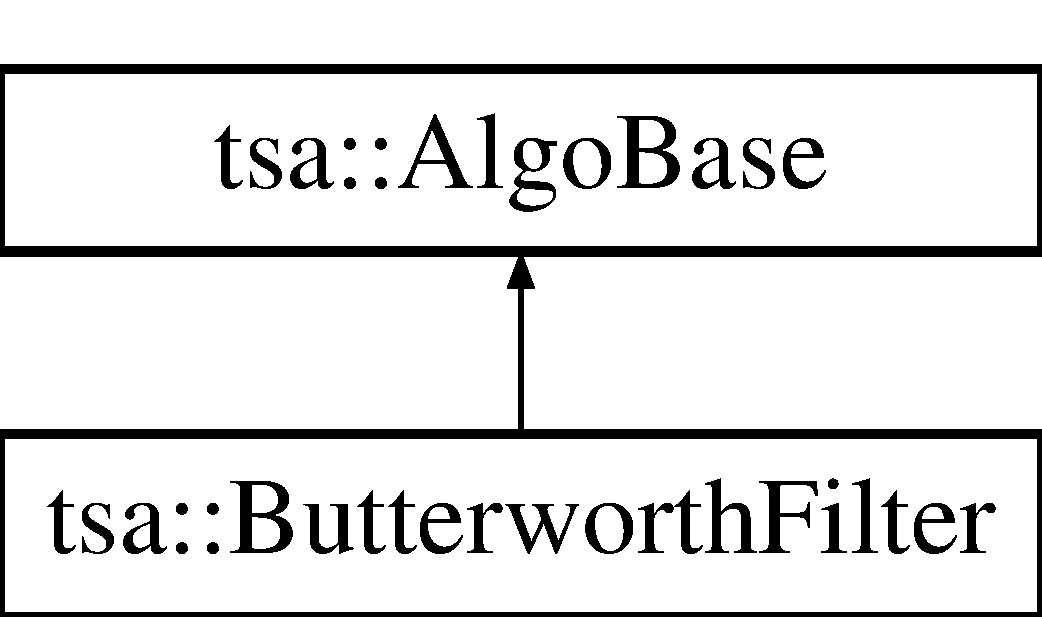
\includegraphics[height=2.000000cm]{classtsa_1_1_butterworth_filter}
\end{center}
\end{figure}
\subsection*{Public Member Functions}
\begin{DoxyCompactItemize}
\item 
\hyperlink{classtsa_1_1_butterworth_filter_a593153a0d04510ed85ddf1464c68dc74}{Butterworth\+Filter} (double freq, int order)
\item 
virtual \hyperlink{classtsa_1_1_butterworth_filter_a085e8ea21b5fb0d564513bca234318df}{$\sim$\+Butterworth\+Filter} ()
\item 
void \hyperlink{classtsa_1_1_butterworth_filter_aa38eef705674e3c799e23bd145d243c0}{operator()} (\hyperlink{namespacetsa_ab32775c889b53c40fa83939f22372b75}{Seq\+View\+Complex} \&data)
\item 
void \hyperlink{classtsa_1_1_butterworth_filter_a68cf85f26d694402fe52601707cf9bbb}{operator()} (\hyperlink{namespacetsa_ab32775c889b53c40fa83939f22372b75}{Seq\+View\+Complex} \&datain, \hyperlink{namespacetsa_ab32775c889b53c40fa83939f22372b75}{Seq\+View\+Complex} \&dataout)
\end{DoxyCompactItemize}
\begin{Indent}\textbf{ Operations}\par
\begin{DoxyCompactItemize}
\item 
void \hyperlink{classtsa_1_1_butterworth_filter_a3e0223e447ec10bd00d488652abb702f}{execute} (\hyperlink{namespacetsa_a86348fef1603a135fe5fba9e5f5486ee}{Cmatrix} \&datain, \hyperlink{namespacetsa_a86348fef1603a135fe5fba9e5f5486ee}{Cmatrix} \&dataout, double fstart, double fsample, double scale)
\item 
void \hyperlink{classtsa_1_1_butterworth_filter_acff437ecb48fcb6cae8865bba97ac533}{execute} (\hyperlink{namespacetsa_a86348fef1603a135fe5fba9e5f5486ee}{Cmatrix} \&datain, double fstart, double fsample, double scale)
\end{DoxyCompactItemize}
\end{Indent}
\subsection*{Private Attributes}
\begin{DoxyCompactItemize}
\item 
int \hyperlink{classtsa_1_1_butterworth_filter_ad81a41345c8b088c6aa02f138b39348b}{m\+Order}
\item 
double \hyperlink{classtsa_1_1_butterworth_filter_a7bff04791bdba8c8b668e8b664f01e60}{m\+Freq}
\item 
\hyperlink{namespacetsa_a7b1f40fa90474b78dd0ab472b7c37547}{Cdouble} $\ast$ \hyperlink{classtsa_1_1_butterworth_filter_a35cbb21e7a98ac4214147afd1aa5b1fe}{poles}
\end{DoxyCompactItemize}


\subsection{Detailed Description}
A generator of random normal numbers. 

Definition at line 74 of file Butterworth\+Filter.\+hpp.



\subsection{Constructor \& Destructor Documentation}
\mbox{\Hypertarget{classtsa_1_1_butterworth_filter_a593153a0d04510ed85ddf1464c68dc74}\label{classtsa_1_1_butterworth_filter_a593153a0d04510ed85ddf1464c68dc74}} 
\index{tsa\+::\+Butterworth\+Filter@{tsa\+::\+Butterworth\+Filter}!Butterworth\+Filter@{Butterworth\+Filter}}
\index{Butterworth\+Filter@{Butterworth\+Filter}!tsa\+::\+Butterworth\+Filter@{tsa\+::\+Butterworth\+Filter}}
\subsubsection{\texorpdfstring{Butterworth\+Filter()}{ButterworthFilter()}}
{\footnotesize\ttfamily tsa\+::\+Butterworth\+Filter\+::\+Butterworth\+Filter (\begin{DoxyParamCaption}\item[{double}]{freq,  }\item[{int}]{order }\end{DoxyParamCaption})}

Constructor 

Definition at line 7 of file Butterworth\+Filter.\+cpp.

\mbox{\Hypertarget{classtsa_1_1_butterworth_filter_a085e8ea21b5fb0d564513bca234318df}\label{classtsa_1_1_butterworth_filter_a085e8ea21b5fb0d564513bca234318df}} 
\index{tsa\+::\+Butterworth\+Filter@{tsa\+::\+Butterworth\+Filter}!````~Butterworth\+Filter@{$\sim$\+Butterworth\+Filter}}
\index{````~Butterworth\+Filter@{$\sim$\+Butterworth\+Filter}!tsa\+::\+Butterworth\+Filter@{tsa\+::\+Butterworth\+Filter}}
\subsubsection{\texorpdfstring{$\sim$\+Butterworth\+Filter()}{~ButterworthFilter()}}
{\footnotesize\ttfamily tsa\+::\+Butterworth\+Filter\+::$\sim$\+Butterworth\+Filter (\begin{DoxyParamCaption}{ }\end{DoxyParamCaption})\hspace{0.3cm}{\ttfamily [virtual]}}

Destructor 

Definition at line 22 of file Butterworth\+Filter.\+cpp.



\subsection{Member Function Documentation}
\mbox{\Hypertarget{classtsa_1_1_butterworth_filter_a3e0223e447ec10bd00d488652abb702f}\label{classtsa_1_1_butterworth_filter_a3e0223e447ec10bd00d488652abb702f}} 
\index{tsa\+::\+Butterworth\+Filter@{tsa\+::\+Butterworth\+Filter}!execute@{execute}}
\index{execute@{execute}!tsa\+::\+Butterworth\+Filter@{tsa\+::\+Butterworth\+Filter}}
\subsubsection{\texorpdfstring{execute()}{execute()}\hspace{0.1cm}{\footnotesize\ttfamily [1/2]}}
{\footnotesize\ttfamily void tsa\+::\+Butterworth\+Filter\+::execute (\begin{DoxyParamCaption}\item[{\hyperlink{namespacetsa_a86348fef1603a135fe5fba9e5f5486ee}{Cmatrix} \&}]{datain,  }\item[{\hyperlink{namespacetsa_a86348fef1603a135fe5fba9e5f5486ee}{Cmatrix} \&}]{dataout,  }\item[{double}]{fstart,  }\item[{double}]{fsample,  }\item[{double}]{scale }\end{DoxyParamCaption})}



Definition at line 79 of file Butterworth\+Filter.\+cpp.

\mbox{\Hypertarget{classtsa_1_1_butterworth_filter_acff437ecb48fcb6cae8865bba97ac533}\label{classtsa_1_1_butterworth_filter_acff437ecb48fcb6cae8865bba97ac533}} 
\index{tsa\+::\+Butterworth\+Filter@{tsa\+::\+Butterworth\+Filter}!execute@{execute}}
\index{execute@{execute}!tsa\+::\+Butterworth\+Filter@{tsa\+::\+Butterworth\+Filter}}
\subsubsection{\texorpdfstring{execute()}{execute()}\hspace{0.1cm}{\footnotesize\ttfamily [2/2]}}
{\footnotesize\ttfamily void tsa\+::\+Butterworth\+Filter\+::execute (\begin{DoxyParamCaption}\item[{\hyperlink{namespacetsa_a86348fef1603a135fe5fba9e5f5486ee}{Cmatrix} \&}]{datain,  }\item[{double}]{fstart,  }\item[{double}]{fsample,  }\item[{double}]{scale }\end{DoxyParamCaption})}



Definition at line 64 of file Butterworth\+Filter.\+cpp.

\mbox{\Hypertarget{classtsa_1_1_butterworth_filter_aa38eef705674e3c799e23bd145d243c0}\label{classtsa_1_1_butterworth_filter_aa38eef705674e3c799e23bd145d243c0}} 
\index{tsa\+::\+Butterworth\+Filter@{tsa\+::\+Butterworth\+Filter}!operator()@{operator()}}
\index{operator()@{operator()}!tsa\+::\+Butterworth\+Filter@{tsa\+::\+Butterworth\+Filter}}
\subsubsection{\texorpdfstring{operator()()}{operator()()}\hspace{0.1cm}{\footnotesize\ttfamily [1/2]}}
{\footnotesize\ttfamily void tsa\+::\+Butterworth\+Filter\+::operator() (\begin{DoxyParamCaption}\item[{\hyperlink{namespacetsa_ab32775c889b53c40fa83939f22372b75}{Seq\+View\+Complex} \&}]{data }\end{DoxyParamCaption})}

Write the filter on a view 

Definition at line 26 of file Butterworth\+Filter.\+cpp.

\mbox{\Hypertarget{classtsa_1_1_butterworth_filter_a68cf85f26d694402fe52601707cf9bbb}\label{classtsa_1_1_butterworth_filter_a68cf85f26d694402fe52601707cf9bbb}} 
\index{tsa\+::\+Butterworth\+Filter@{tsa\+::\+Butterworth\+Filter}!operator()@{operator()}}
\index{operator()@{operator()}!tsa\+::\+Butterworth\+Filter@{tsa\+::\+Butterworth\+Filter}}
\subsubsection{\texorpdfstring{operator()()}{operator()()}\hspace{0.1cm}{\footnotesize\ttfamily [2/2]}}
{\footnotesize\ttfamily void tsa\+::\+Butterworth\+Filter\+::operator() (\begin{DoxyParamCaption}\item[{\hyperlink{namespacetsa_ab32775c889b53c40fa83939f22372b75}{Seq\+View\+Complex} \&}]{datain,  }\item[{\hyperlink{namespacetsa_ab32775c889b53c40fa83939f22372b75}{Seq\+View\+Complex} \&}]{dataout }\end{DoxyParamCaption})}

Apply the filter on a view 

Definition at line 43 of file Butterworth\+Filter.\+cpp.



\subsection{Member Data Documentation}
\mbox{\Hypertarget{classtsa_1_1_butterworth_filter_a7bff04791bdba8c8b668e8b664f01e60}\label{classtsa_1_1_butterworth_filter_a7bff04791bdba8c8b668e8b664f01e60}} 
\index{tsa\+::\+Butterworth\+Filter@{tsa\+::\+Butterworth\+Filter}!m\+Freq@{m\+Freq}}
\index{m\+Freq@{m\+Freq}!tsa\+::\+Butterworth\+Filter@{tsa\+::\+Butterworth\+Filter}}
\subsubsection{\texorpdfstring{m\+Freq}{mFreq}}
{\footnotesize\ttfamily double tsa\+::\+Butterworth\+Filter\+::m\+Freq\hspace{0.3cm}{\ttfamily [private]}}



Definition at line 137 of file Butterworth\+Filter.\+hpp.

\mbox{\Hypertarget{classtsa_1_1_butterworth_filter_ad81a41345c8b088c6aa02f138b39348b}\label{classtsa_1_1_butterworth_filter_ad81a41345c8b088c6aa02f138b39348b}} 
\index{tsa\+::\+Butterworth\+Filter@{tsa\+::\+Butterworth\+Filter}!m\+Order@{m\+Order}}
\index{m\+Order@{m\+Order}!tsa\+::\+Butterworth\+Filter@{tsa\+::\+Butterworth\+Filter}}
\subsubsection{\texorpdfstring{m\+Order}{mOrder}}
{\footnotesize\ttfamily int tsa\+::\+Butterworth\+Filter\+::m\+Order\hspace{0.3cm}{\ttfamily [private]}}



Definition at line 136 of file Butterworth\+Filter.\+hpp.

\mbox{\Hypertarget{classtsa_1_1_butterworth_filter_a35cbb21e7a98ac4214147afd1aa5b1fe}\label{classtsa_1_1_butterworth_filter_a35cbb21e7a98ac4214147afd1aa5b1fe}} 
\index{tsa\+::\+Butterworth\+Filter@{tsa\+::\+Butterworth\+Filter}!poles@{poles}}
\index{poles@{poles}!tsa\+::\+Butterworth\+Filter@{tsa\+::\+Butterworth\+Filter}}
\subsubsection{\texorpdfstring{poles}{poles}}
{\footnotesize\ttfamily \hyperlink{namespacetsa_a7b1f40fa90474b78dd0ab472b7c37547}{Cdouble}$\ast$ tsa\+::\+Butterworth\+Filter\+::poles\hspace{0.3cm}{\ttfamily [private]}}



Definition at line 138 of file Butterworth\+Filter.\+hpp.



The documentation for this class was generated from the following files\+:\begin{DoxyCompactItemize}
\item 
/home/filip/\+Ph\+D/\+W\+D\+F\+Pipe\+\_\+test/p4\+T\+S\+A/include/\hyperlink{_butterworth_filter_8hpp}{Butterworth\+Filter.\+hpp}\item 
/home/filip/\+Ph\+D/\+W\+D\+F\+Pipe\+\_\+test/p4\+T\+S\+A/src/\hyperlink{_butterworth_filter_8cpp}{Butterworth\+Filter.\+cpp}\end{DoxyCompactItemize}

\hypertarget{classtsa_1_1_channel_descriptor}{}\section{tsa\+:\+:Channel\+Descriptor Class Reference}
\label{classtsa_1_1_channel_descriptor}\index{tsa\+::\+Channel\+Descriptor@{tsa\+::\+Channel\+Descriptor}}


{\ttfamily \#include $<$Frame\+I\+Stream.\+hpp$>$}

Inheritance diagram for tsa\+:\+:Channel\+Descriptor\+:\begin{figure}[H]
\begin{center}
\leavevmode
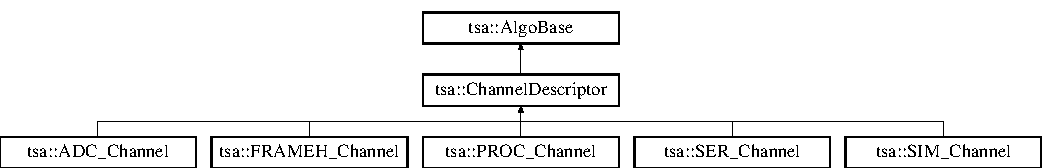
\includegraphics[height=2.255033cm]{classtsa_1_1_channel_descriptor}
\end{center}
\end{figure}
\subsection*{Public Member Functions}
\begin{DoxyCompactItemize}
\item 
\hyperlink{classtsa_1_1_channel_descriptor_a320624e156e5d856077465474bc7154f}{Channel\+Descriptor} (unsigned int id)
\item 
virtual void \hyperlink{classtsa_1_1_channel_descriptor_aa1e001a5e712415cd4e9d66846914a56}{Add\+Data} ()
\item 
virtual double \hyperlink{classtsa_1_1_channel_descriptor_a456d14e6136c389fbd307fabab7d7b73}{Get\+Length} ()
\item 
virtual double \hyperlink{classtsa_1_1_channel_descriptor_a602c501d3fa47c0951ae45f78336a1a8}{Get\+Rate} ()
\item 
virtual void \hyperlink{classtsa_1_1_channel_descriptor_a5ebd9a8bf358666b2cd9ae00056d2728}{Write\+View} (\hyperlink{namespacetsa_ac599574bcc094eda25613724b8f3ca9e}{Seq\+View\+Double} \&v)
\item 
virtual void \hyperlink{classtsa_1_1_channel_descriptor_a6553da04ba33471fc5465b6bd2b5275c}{Fill\+View} (\hyperlink{namespacetsa_ac599574bcc094eda25613724b8f3ca9e}{Seq\+View\+Double} \&v, double tstart, double tend)
\item 
virtual void \hyperlink{classtsa_1_1_channel_descriptor_a51b2df6d09b5b0b07d2a9ecda6fffa2b}{Write\+View} (\hyperlink{namespacetsa_ac599574bcc094eda25613724b8f3ca9e}{Seq\+View\+Double} \&v, \hyperlink{namespacetsa_ac599574bcc094eda25613724b8f3ca9e}{Seq\+View\+Double} \&validation)
\item 
virtual \hyperlink{classtsa_1_1_channel_descriptor_a2b4f201421dcd2cc9d2c1705fe4bea61}{$\sim$\+Channel\+Descriptor} ()
\end{DoxyCompactItemize}
\subsection*{Protected Member Functions}
\begin{DoxyCompactItemize}
\item 
void \hyperlink{classtsa_1_1_channel_descriptor_ae3da8cb574d6a43bcca33daca5394530}{Push\+Value} (double value, double t, unsigned int n)
\item 
void \hyperlink{classtsa_1_1_channel_descriptor_a61cb9c3f50762989afc59c9e365f0927}{Push\+Fr\+Vect} (Fr\+Vect $\ast$frv, double t, unsigned int off, double offset, double slope)
\item 
void \hyperlink{classtsa_1_1_channel_descriptor_ae38a3b6ca5d23123a61a421fe3612b86}{Queue} (double v, double t)
\item 
bool \hyperlink{classtsa_1_1_channel_descriptor_a73d060e190a75faa7ac64ee4a328a9d4}{data\+\_\+available} (double t)
\end{DoxyCompactItemize}
\subsection*{Protected Attributes}
\begin{DoxyCompactItemize}
\item 
\hyperlink{classtsa_1_1_frame_i_stream}{Frame\+I\+Stream} $\ast$ \hyperlink{classtsa_1_1_channel_descriptor_a7767947e90a66d41bbd13bd4c54149a6}{m\+F\+IS}
\item 
unsigned int \hyperlink{classtsa_1_1_channel_descriptor_a49d1e3852cb22b0a56ebc03b3176c5b8}{m\+Id}
\item 
double \hyperlink{classtsa_1_1_channel_descriptor_a142c7f60e14fa8036340b902529cf956}{m\+Rate}
\item 
double \hyperlink{classtsa_1_1_channel_descriptor_a6bad409238df7dff8b5265570adac8ff}{m\+Next\+Time}
\item 
std\+::deque$<$ double $>$ \hyperlink{classtsa_1_1_channel_descriptor_ad1568c18971efe9a5cb1d114e06f5050}{m\+Data}
\item 
std\+::deque$<$ \hyperlink{structtsa_1_1_data_exception}{Data\+Exception} $>$ \hyperlink{classtsa_1_1_channel_descriptor_ac4103a2793b7e507f8f982070ee27348}{m\+Exceptions}
\end{DoxyCompactItemize}


\subsection{Detailed Description}
A base class for the descriptor of a data channel. 

Definition at line 101 of file Frame\+I\+Stream.\+hpp.



\subsection{Constructor \& Destructor Documentation}
\mbox{\Hypertarget{classtsa_1_1_channel_descriptor_a320624e156e5d856077465474bc7154f}\label{classtsa_1_1_channel_descriptor_a320624e156e5d856077465474bc7154f}} 
\index{tsa\+::\+Channel\+Descriptor@{tsa\+::\+Channel\+Descriptor}!Channel\+Descriptor@{Channel\+Descriptor}}
\index{Channel\+Descriptor@{Channel\+Descriptor}!tsa\+::\+Channel\+Descriptor@{tsa\+::\+Channel\+Descriptor}}
\subsubsection{\texorpdfstring{Channel\+Descriptor()}{ChannelDescriptor()}}
{\footnotesize\ttfamily tsa\+::\+Channel\+Descriptor\+::\+Channel\+Descriptor (\begin{DoxyParamCaption}\item[{unsigned int}]{id }\end{DoxyParamCaption})\hspace{0.3cm}{\ttfamily [inline]}}

Constructor.


\begin{DoxyParams}{Parameters}
{\em id} & number of data channel \\
\hline
\end{DoxyParams}


Definition at line 110 of file Frame\+I\+Stream.\+hpp.

\mbox{\Hypertarget{classtsa_1_1_channel_descriptor_a2b4f201421dcd2cc9d2c1705fe4bea61}\label{classtsa_1_1_channel_descriptor_a2b4f201421dcd2cc9d2c1705fe4bea61}} 
\index{tsa\+::\+Channel\+Descriptor@{tsa\+::\+Channel\+Descriptor}!````~Channel\+Descriptor@{$\sim$\+Channel\+Descriptor}}
\index{````~Channel\+Descriptor@{$\sim$\+Channel\+Descriptor}!tsa\+::\+Channel\+Descriptor@{tsa\+::\+Channel\+Descriptor}}
\subsubsection{\texorpdfstring{$\sim$\+Channel\+Descriptor()}{~ChannelDescriptor()}}
{\footnotesize\ttfamily virtual tsa\+::\+Channel\+Descriptor\+::$\sim$\+Channel\+Descriptor (\begin{DoxyParamCaption}{ }\end{DoxyParamCaption})\hspace{0.3cm}{\ttfamily [inline]}, {\ttfamily [virtual]}}

Destructor 

Definition at line 167 of file Frame\+I\+Stream.\+hpp.



\subsection{Member Function Documentation}
\mbox{\Hypertarget{classtsa_1_1_channel_descriptor_aa1e001a5e712415cd4e9d66846914a56}\label{classtsa_1_1_channel_descriptor_aa1e001a5e712415cd4e9d66846914a56}} 
\index{tsa\+::\+Channel\+Descriptor@{tsa\+::\+Channel\+Descriptor}!Add\+Data@{Add\+Data}}
\index{Add\+Data@{Add\+Data}!tsa\+::\+Channel\+Descriptor@{tsa\+::\+Channel\+Descriptor}}
\subsubsection{\texorpdfstring{Add\+Data()}{AddData()}}
{\footnotesize\ttfamily virtual void tsa\+::\+Channel\+Descriptor\+::\+Add\+Data (\begin{DoxyParamCaption}{ }\end{DoxyParamCaption})\hspace{0.3cm}{\ttfamily [inline]}, {\ttfamily [virtual]}}

This function must be called when there are not enough data to fill the output view. In this base class does nothing. 

Reimplemented in \hyperlink{classtsa_1_1_f_r_a_m_e_h___channel_af757e23c465da95ac0ed7b97876ead66}{tsa\+::\+F\+R\+A\+M\+E\+H\+\_\+\+Channel}, \hyperlink{classtsa_1_1_s_e_r___channel_a77efdde9aaa7bbd356088bb1c15e59bf}{tsa\+::\+S\+E\+R\+\_\+\+Channel}, \hyperlink{classtsa_1_1_s_i_m___channel_ada133d83befff9b1bde7e13bb78df7e0}{tsa\+::\+S\+I\+M\+\_\+\+Channel}, \hyperlink{classtsa_1_1_p_r_o_c___channel_ab4f986f7829c52ca6c0d8c244be7c617}{tsa\+::\+P\+R\+O\+C\+\_\+\+Channel}, and \hyperlink{classtsa_1_1_a_d_c___channel_a23052bc47591e46246701ec0573c7902}{tsa\+::\+A\+D\+C\+\_\+\+Channel}.



Definition at line 118 of file Frame\+I\+Stream.\+hpp.

\mbox{\Hypertarget{classtsa_1_1_channel_descriptor_a73d060e190a75faa7ac64ee4a328a9d4}\label{classtsa_1_1_channel_descriptor_a73d060e190a75faa7ac64ee4a328a9d4}} 
\index{tsa\+::\+Channel\+Descriptor@{tsa\+::\+Channel\+Descriptor}!data\+\_\+available@{data\+\_\+available}}
\index{data\+\_\+available@{data\+\_\+available}!tsa\+::\+Channel\+Descriptor@{tsa\+::\+Channel\+Descriptor}}
\subsubsection{\texorpdfstring{data\+\_\+available()}{data\_available()}}
{\footnotesize\ttfamily bool tsa\+::\+Channel\+Descriptor\+::data\+\_\+available (\begin{DoxyParamCaption}\item[{double}]{t }\end{DoxyParamCaption})\hspace{0.3cm}{\ttfamily [protected]}}

Check the availability of a value at a given time, looking in the set of registered data losses. Remove from this set all the exceptions which correspond to times lower than t.


\begin{DoxyParams}{Parameters}
{\em t} & requested time\\
\hline
\end{DoxyParams}
\begin{DoxyReturn}{Returns}
true if a number is available at the given time, false otherwise 
\end{DoxyReturn}


Definition at line 125 of file Frame\+I\+Stream.\+cpp.

\mbox{\Hypertarget{classtsa_1_1_channel_descriptor_a6553da04ba33471fc5465b6bd2b5275c}\label{classtsa_1_1_channel_descriptor_a6553da04ba33471fc5465b6bd2b5275c}} 
\index{tsa\+::\+Channel\+Descriptor@{tsa\+::\+Channel\+Descriptor}!Fill\+View@{Fill\+View}}
\index{Fill\+View@{Fill\+View}!tsa\+::\+Channel\+Descriptor@{tsa\+::\+Channel\+Descriptor}}
\subsubsection{\texorpdfstring{Fill\+View()}{FillView()}}
{\footnotesize\ttfamily void tsa\+::\+Channel\+Descriptor\+::\+Fill\+View (\begin{DoxyParamCaption}\item[{\hyperlink{namespacetsa_ac599574bcc094eda25613724b8f3ca9e}{Seq\+View\+Double} \&}]{v,  }\item[{double}]{tstart,  }\item[{double}]{tend }\end{DoxyParamCaption})\hspace{0.3cm}{\ttfamily [virtual]}}



Reimplemented in \hyperlink{classtsa_1_1_p_r_o_c___channel_a84f00b22077b0aa41dba95ac0aaf0478}{tsa\+::\+P\+R\+O\+C\+\_\+\+Channel}.



Definition at line 176 of file Frame\+I\+Stream.\+cpp.

\mbox{\Hypertarget{classtsa_1_1_channel_descriptor_a456d14e6136c389fbd307fabab7d7b73}\label{classtsa_1_1_channel_descriptor_a456d14e6136c389fbd307fabab7d7b73}} 
\index{tsa\+::\+Channel\+Descriptor@{tsa\+::\+Channel\+Descriptor}!Get\+Length@{Get\+Length}}
\index{Get\+Length@{Get\+Length}!tsa\+::\+Channel\+Descriptor@{tsa\+::\+Channel\+Descriptor}}
\subsubsection{\texorpdfstring{Get\+Length()}{GetLength()}}
{\footnotesize\ttfamily virtual double tsa\+::\+Channel\+Descriptor\+::\+Get\+Length (\begin{DoxyParamCaption}{ }\end{DoxyParamCaption})\hspace{0.3cm}{\ttfamily [inline]}, {\ttfamily [virtual]}}

Get the maximul time length of data that can be currently filled without calling Add\+Data.

\begin{DoxyReturn}{Returns}
the time length of the data available in seconds 
\end{DoxyReturn}


Reimplemented in \hyperlink{classtsa_1_1_f_r_a_m_e_h___channel_a022b134fb62d99e8cb00a6ce28b2d569}{tsa\+::\+F\+R\+A\+M\+E\+H\+\_\+\+Channel}, \hyperlink{classtsa_1_1_s_e_r___channel_ac2cb2ded2f417590ed1da5c5e2315569}{tsa\+::\+S\+E\+R\+\_\+\+Channel}, \hyperlink{classtsa_1_1_s_i_m___channel_a99941fc8df0c8bbc32091e7e87d20de8}{tsa\+::\+S\+I\+M\+\_\+\+Channel}, \hyperlink{classtsa_1_1_p_r_o_c___channel_ac29ae55cbededca3814b30e1186a4650}{tsa\+::\+P\+R\+O\+C\+\_\+\+Channel}, and \hyperlink{classtsa_1_1_a_d_c___channel_ab5e23c219a7bf70866b05c9d3ad3da6f}{tsa\+::\+A\+D\+C\+\_\+\+Channel}.



Definition at line 127 of file Frame\+I\+Stream.\+hpp.

\mbox{\Hypertarget{classtsa_1_1_channel_descriptor_a602c501d3fa47c0951ae45f78336a1a8}\label{classtsa_1_1_channel_descriptor_a602c501d3fa47c0951ae45f78336a1a8}} 
\index{tsa\+::\+Channel\+Descriptor@{tsa\+::\+Channel\+Descriptor}!Get\+Rate@{Get\+Rate}}
\index{Get\+Rate@{Get\+Rate}!tsa\+::\+Channel\+Descriptor@{tsa\+::\+Channel\+Descriptor}}
\subsubsection{\texorpdfstring{Get\+Rate()}{GetRate()}}
{\footnotesize\ttfamily virtual double tsa\+::\+Channel\+Descriptor\+::\+Get\+Rate (\begin{DoxyParamCaption}{ }\end{DoxyParamCaption})\hspace{0.3cm}{\ttfamily [inline]}, {\ttfamily [virtual]}}

Get the channel time rate

\begin{DoxyReturn}{Returns}
the channel time rate 
\end{DoxyReturn}


Definition at line 137 of file Frame\+I\+Stream.\+hpp.

\mbox{\Hypertarget{classtsa_1_1_channel_descriptor_a61cb9c3f50762989afc59c9e365f0927}\label{classtsa_1_1_channel_descriptor_a61cb9c3f50762989afc59c9e365f0927}} 
\index{tsa\+::\+Channel\+Descriptor@{tsa\+::\+Channel\+Descriptor}!Push\+Fr\+Vect@{Push\+Fr\+Vect}}
\index{Push\+Fr\+Vect@{Push\+Fr\+Vect}!tsa\+::\+Channel\+Descriptor@{tsa\+::\+Channel\+Descriptor}}
\subsubsection{\texorpdfstring{Push\+Fr\+Vect()}{PushFrVect()}}
{\footnotesize\ttfamily void tsa\+::\+Channel\+Descriptor\+::\+Push\+Fr\+Vect (\begin{DoxyParamCaption}\item[{Fr\+Vect $\ast$}]{frv,  }\item[{double}]{t,  }\item[{unsigned int}]{off,  }\item[{double}]{offset,  }\item[{double}]{slope }\end{DoxyParamCaption})\hspace{0.3cm}{\ttfamily [protected]}}

Call \begin{DoxySeeAlso}{See also}
\hyperlink{classtsa_1_1_channel_descriptor_ae38a3b6ca5d23123a61a421fe3612b86}{Queue} for a sequence of numerical values. The values are contained inside a Fr\+Vect, starting from a given offset. The effective value which is passed to 

\hyperlink{classtsa_1_1_channel_descriptor_ae38a3b6ca5d23123a61a421fe3612b86}{Queue} is given by y=offset+slope$\ast$x, where x is the value contained in the Fr\+Vect.
\end{DoxySeeAlso}

\begin{DoxyParams}{Parameters}
{\em frv} & pointer to the Fr\+Vect containing data \\
\hline
{\em t} & time corresponding to the first data contained in the Fr\+Vect (neglecting the offset) \\
\hline
{\em off} & offset in the Fr\+Vect \\
\hline
{\em offset} & an optional offset to correct the data \\
\hline
{\em slope} & an optional scaling factor to correct the data \\
\hline
\end{DoxyParams}


Definition at line 66 of file Frame\+I\+Stream.\+cpp.

\mbox{\Hypertarget{classtsa_1_1_channel_descriptor_ae3da8cb574d6a43bcca33daca5394530}\label{classtsa_1_1_channel_descriptor_ae3da8cb574d6a43bcca33daca5394530}} 
\index{tsa\+::\+Channel\+Descriptor@{tsa\+::\+Channel\+Descriptor}!Push\+Value@{Push\+Value}}
\index{Push\+Value@{Push\+Value}!tsa\+::\+Channel\+Descriptor@{tsa\+::\+Channel\+Descriptor}}
\subsubsection{\texorpdfstring{Push\+Value()}{PushValue()}}
{\footnotesize\ttfamily void tsa\+::\+Channel\+Descriptor\+::\+Push\+Value (\begin{DoxyParamCaption}\item[{double}]{value,  }\item[{double}]{t,  }\item[{unsigned int}]{n }\end{DoxyParamCaption})\hspace{0.3cm}{\ttfamily [protected]}}

Call \begin{DoxySeeAlso}{See also}
\hyperlink{classtsa_1_1_channel_descriptor_ae38a3b6ca5d23123a61a421fe3612b86}{Queue} n times, passing the given value and the corresponding time.
\end{DoxySeeAlso}

\begin{DoxyParams}{Parameters}
{\em value} & the value that must be added to the queue \\
\hline
{\em t} & the time which correspond to the data \\
\hline
{\em n} & number of copies of the data that must be added \\
\hline
\end{DoxyParams}


Definition at line 60 of file Frame\+I\+Stream.\+cpp.

\mbox{\Hypertarget{classtsa_1_1_channel_descriptor_ae38a3b6ca5d23123a61a421fe3612b86}\label{classtsa_1_1_channel_descriptor_ae38a3b6ca5d23123a61a421fe3612b86}} 
\index{tsa\+::\+Channel\+Descriptor@{tsa\+::\+Channel\+Descriptor}!Queue@{Queue}}
\index{Queue@{Queue}!tsa\+::\+Channel\+Descriptor@{tsa\+::\+Channel\+Descriptor}}
\subsubsection{\texorpdfstring{Queue()}{Queue()}}
{\footnotesize\ttfamily void tsa\+::\+Channel\+Descriptor\+::\+Queue (\begin{DoxyParamCaption}\item[{double}]{v,  }\item[{double}]{t }\end{DoxyParamCaption})\hspace{0.3cm}{\ttfamily [protected]}}

Push a given value v, at the given time t, in the output queue. The value is pushed only if its time is larger or equal that the current m\+Next\+Time. If it is larger that the current m\+Next\+Time value a data loss is registered.

The value of m\+Next\+Time is updated.


\begin{DoxyParams}{Parameters}
{\em v} & the value \\
\hline
{\em t} & the time \\
\hline
\end{DoxyParams}


Definition at line 34 of file Frame\+I\+Stream.\+cpp.

\mbox{\Hypertarget{classtsa_1_1_channel_descriptor_a5ebd9a8bf358666b2cd9ae00056d2728}\label{classtsa_1_1_channel_descriptor_a5ebd9a8bf358666b2cd9ae00056d2728}} 
\index{tsa\+::\+Channel\+Descriptor@{tsa\+::\+Channel\+Descriptor}!Write\+View@{Write\+View}}
\index{Write\+View@{Write\+View}!tsa\+::\+Channel\+Descriptor@{tsa\+::\+Channel\+Descriptor}}
\subsubsection{\texorpdfstring{Write\+View()}{WriteView()}\hspace{0.1cm}{\footnotesize\ttfamily [1/2]}}
{\footnotesize\ttfamily void tsa\+::\+Channel\+Descriptor\+::\+Write\+View (\begin{DoxyParamCaption}\item[{\hyperlink{namespacetsa_ac599574bcc094eda25613724b8f3ca9e}{Seq\+View\+Double} \&}]{v }\end{DoxyParamCaption})\hspace{0.3cm}{\ttfamily [virtual]}}

A function to write the available data on an output view. Be careful that if there are not enough data available we get a data loss exception.


\begin{DoxyParams}{Parameters}
{\em v} & output view where the available data are written \\
\hline
\end{DoxyParams}


Definition at line 149 of file Frame\+I\+Stream.\+cpp.

\mbox{\Hypertarget{classtsa_1_1_channel_descriptor_a51b2df6d09b5b0b07d2a9ecda6fffa2b}\label{classtsa_1_1_channel_descriptor_a51b2df6d09b5b0b07d2a9ecda6fffa2b}} 
\index{tsa\+::\+Channel\+Descriptor@{tsa\+::\+Channel\+Descriptor}!Write\+View@{Write\+View}}
\index{Write\+View@{Write\+View}!tsa\+::\+Channel\+Descriptor@{tsa\+::\+Channel\+Descriptor}}
\subsubsection{\texorpdfstring{Write\+View()}{WriteView()}\hspace{0.1cm}{\footnotesize\ttfamily [2/2]}}
{\footnotesize\ttfamily void tsa\+::\+Channel\+Descriptor\+::\+Write\+View (\begin{DoxyParamCaption}\item[{\hyperlink{namespacetsa_ac599574bcc094eda25613724b8f3ca9e}{Seq\+View\+Double} \&}]{v,  }\item[{\hyperlink{namespacetsa_ac599574bcc094eda25613724b8f3ca9e}{Seq\+View\+Double} \&}]{validation }\end{DoxyParamCaption})\hspace{0.3cm}{\ttfamily [virtual]}}

A function to write the available data on an output view. Be careful that if there are not enough data available we get a data loss exception. At the same time a second view is filled with ones which correspond to avaliable data, or zeros which correspond to unavailable data.


\begin{DoxyParams}{Parameters}
{\em v} & output view where the available data are written \\
\hline
{\em validation} & output view where the available data flags are written \\
\hline
\end{DoxyParams}


Definition at line 180 of file Frame\+I\+Stream.\+cpp.



\subsection{Member Data Documentation}
\mbox{\Hypertarget{classtsa_1_1_channel_descriptor_ad1568c18971efe9a5cb1d114e06f5050}\label{classtsa_1_1_channel_descriptor_ad1568c18971efe9a5cb1d114e06f5050}} 
\index{tsa\+::\+Channel\+Descriptor@{tsa\+::\+Channel\+Descriptor}!m\+Data@{m\+Data}}
\index{m\+Data@{m\+Data}!tsa\+::\+Channel\+Descriptor@{tsa\+::\+Channel\+Descriptor}}
\subsubsection{\texorpdfstring{m\+Data}{mData}}
{\footnotesize\ttfamily std\+::deque$<$double$>$ tsa\+::\+Channel\+Descriptor\+::m\+Data\hspace{0.3cm}{\ttfamily [protected]}}

The data queue 

Definition at line 222 of file Frame\+I\+Stream.\+hpp.

\mbox{\Hypertarget{classtsa_1_1_channel_descriptor_ac4103a2793b7e507f8f982070ee27348}\label{classtsa_1_1_channel_descriptor_ac4103a2793b7e507f8f982070ee27348}} 
\index{tsa\+::\+Channel\+Descriptor@{tsa\+::\+Channel\+Descriptor}!m\+Exceptions@{m\+Exceptions}}
\index{m\+Exceptions@{m\+Exceptions}!tsa\+::\+Channel\+Descriptor@{tsa\+::\+Channel\+Descriptor}}
\subsubsection{\texorpdfstring{m\+Exceptions}{mExceptions}}
{\footnotesize\ttfamily std\+::deque$<$\hyperlink{structtsa_1_1_data_exception}{Data\+Exception}$>$ tsa\+::\+Channel\+Descriptor\+::m\+Exceptions\hspace{0.3cm}{\ttfamily [protected]}}

The set of data loss exceptions 

Definition at line 223 of file Frame\+I\+Stream.\+hpp.

\mbox{\Hypertarget{classtsa_1_1_channel_descriptor_a7767947e90a66d41bbd13bd4c54149a6}\label{classtsa_1_1_channel_descriptor_a7767947e90a66d41bbd13bd4c54149a6}} 
\index{tsa\+::\+Channel\+Descriptor@{tsa\+::\+Channel\+Descriptor}!m\+F\+IS@{m\+F\+IS}}
\index{m\+F\+IS@{m\+F\+IS}!tsa\+::\+Channel\+Descriptor@{tsa\+::\+Channel\+Descriptor}}
\subsubsection{\texorpdfstring{m\+F\+IS}{mFIS}}
{\footnotesize\ttfamily \hyperlink{classtsa_1_1_frame_i_stream}{Frame\+I\+Stream}$\ast$ tsa\+::\+Channel\+Descriptor\+::m\+F\+IS\hspace{0.3cm}{\ttfamily [protected]}}

Pointer to the \hyperlink{classtsa_1_1_frame_i_stream}{Frame\+I\+Stream} class which contains this descriptor 

Definition at line 218 of file Frame\+I\+Stream.\+hpp.

\mbox{\Hypertarget{classtsa_1_1_channel_descriptor_a49d1e3852cb22b0a56ebc03b3176c5b8}\label{classtsa_1_1_channel_descriptor_a49d1e3852cb22b0a56ebc03b3176c5b8}} 
\index{tsa\+::\+Channel\+Descriptor@{tsa\+::\+Channel\+Descriptor}!m\+Id@{m\+Id}}
\index{m\+Id@{m\+Id}!tsa\+::\+Channel\+Descriptor@{tsa\+::\+Channel\+Descriptor}}
\subsubsection{\texorpdfstring{m\+Id}{mId}}
{\footnotesize\ttfamily unsigned int tsa\+::\+Channel\+Descriptor\+::m\+Id\hspace{0.3cm}{\ttfamily [protected]}}

The numerical id of the class 

Definition at line 219 of file Frame\+I\+Stream.\+hpp.

\mbox{\Hypertarget{classtsa_1_1_channel_descriptor_a6bad409238df7dff8b5265570adac8ff}\label{classtsa_1_1_channel_descriptor_a6bad409238df7dff8b5265570adac8ff}} 
\index{tsa\+::\+Channel\+Descriptor@{tsa\+::\+Channel\+Descriptor}!m\+Next\+Time@{m\+Next\+Time}}
\index{m\+Next\+Time@{m\+Next\+Time}!tsa\+::\+Channel\+Descriptor@{tsa\+::\+Channel\+Descriptor}}
\subsubsection{\texorpdfstring{m\+Next\+Time}{mNextTime}}
{\footnotesize\ttfamily double tsa\+::\+Channel\+Descriptor\+::m\+Next\+Time\hspace{0.3cm}{\ttfamily [protected]}}

The time at which the next data to push on the queue is expected 

Definition at line 221 of file Frame\+I\+Stream.\+hpp.

\mbox{\Hypertarget{classtsa_1_1_channel_descriptor_a142c7f60e14fa8036340b902529cf956}\label{classtsa_1_1_channel_descriptor_a142c7f60e14fa8036340b902529cf956}} 
\index{tsa\+::\+Channel\+Descriptor@{tsa\+::\+Channel\+Descriptor}!m\+Rate@{m\+Rate}}
\index{m\+Rate@{m\+Rate}!tsa\+::\+Channel\+Descriptor@{tsa\+::\+Channel\+Descriptor}}
\subsubsection{\texorpdfstring{m\+Rate}{mRate}}
{\footnotesize\ttfamily double tsa\+::\+Channel\+Descriptor\+::m\+Rate\hspace{0.3cm}{\ttfamily [protected]}}

The rate of the data 

Definition at line 220 of file Frame\+I\+Stream.\+hpp.



The documentation for this class was generated from the following files\+:\begin{DoxyCompactItemize}
\item 
/home/filip/\+Ph\+D/\+W\+D\+F\+Pipe\+\_\+test/p4\+T\+S\+A/include/\hyperlink{_frame_i_stream_8hpp}{Frame\+I\+Stream.\+hpp}\item 
/home/filip/\+Ph\+D/\+W\+D\+F\+Pipe\+\_\+test/p4\+T\+S\+A/src/\hyperlink{_frame_i_stream_8cpp}{Frame\+I\+Stream.\+cpp}\end{DoxyCompactItemize}

\hypertarget{classtsa_1_1_cholesky}{}\section{tsa\+:\+:Cholesky Class Reference}
\label{classtsa_1_1_cholesky}\index{tsa\+::\+Cholesky@{tsa\+::\+Cholesky}}


{\ttfamily \#include $<$Cholesky.\+hpp$>$}

\subsection*{Public Member Functions}
\begin{DoxyCompactItemize}
\item 
\hyperlink{classtsa_1_1_cholesky_a19dfa3cb6bf14721a91ec6fdcb26dbcf}{Cholesky} (unsigned int N, double eps)
\item 
\hyperlink{classtsa_1_1_cholesky_a86a264d92076daba27859959741b3627}{Cholesky} (const \hyperlink{classtsa_1_1_cholesky}{Cholesky} \&from)
\item 
\hyperlink{classtsa_1_1_cholesky_a45d30ca313f3949504716bacb5036b6d}{$\sim$\+Cholesky} ()
\item 
\hyperlink{classtsa_1_1_cholesky}{Cholesky} \& \hyperlink{classtsa_1_1_cholesky_a3c86b3ab61a3dd759b067ce685e6f51e}{operator=} (const \hyperlink{classtsa_1_1_cholesky}{Cholesky} \&from)
\end{DoxyCompactItemize}
\begin{Indent}\textbf{ Operations}\par
\begin{DoxyCompactItemize}
\item 
void \hyperlink{classtsa_1_1_cholesky_ac04746ca67f2fb532dc060a35a1ba4d8}{execute} (\hyperlink{namespacetsa_a8900fb03d849baf447a1a0efe2561fb2}{Dvector} \&A, \hyperlink{namespacetsa_a8900fb03d849baf447a1a0efe2561fb2}{Dvector} \&B)
\begin{DoxyCompactList}\small\item\em Brief documentation for the execute method. \end{DoxyCompactList}\end{DoxyCompactItemize}
\end{Indent}
\subsection*{Private Attributes}
\begin{DoxyCompactItemize}
\item 
unsigned int \hyperlink{classtsa_1_1_cholesky_aeebdfa1ac318dceb73fccfe75f3928bc}{mN}
\item 
\hyperlink{namespacetsa_a8900fb03d849baf447a1a0efe2561fb2}{Dvector} \hyperlink{classtsa_1_1_cholesky_afb8463f2c148c8ae2ef2c2914074718a}{mD}
\item 
\hyperlink{namespacetsa_a8900fb03d849baf447a1a0efe2561fb2}{Dvector} \hyperlink{classtsa_1_1_cholesky_a71ce7b253e3824f3629ca31ba049f58e}{mY}
\item 
\hyperlink{namespacetsa_ad260cd21c1891c4ed391fe788569aba4}{Dmatrix} \hyperlink{classtsa_1_1_cholesky_a56d3135a9c56e030e9cf876fd99dbbc3}{m\+XL}
\item 
int \hyperlink{classtsa_1_1_cholesky_afc88d4ebf8b5a163a77ef3e3dd90f99d}{m\+Iflag}
\item 
double \hyperlink{classtsa_1_1_cholesky_aa49812e981a177f6792389d0d760db52}{m\+Eps}
\end{DoxyCompactItemize}


\subsection{Detailed Description}
Perform the \hyperlink{classtsa_1_1_cholesky}{Cholesky} decomposition

\begin{DoxyAuthor}{Author}
Elena Cuoco \href{mailto:elena.cuoco@ego-gw.it}{\tt elena.\+cuoco@ego-\/gw.\+it} 
\end{DoxyAuthor}


Definition at line 78 of file Cholesky.\+hpp.



\subsection{Constructor \& Destructor Documentation}
\mbox{\Hypertarget{classtsa_1_1_cholesky_a19dfa3cb6bf14721a91ec6fdcb26dbcf}\label{classtsa_1_1_cholesky_a19dfa3cb6bf14721a91ec6fdcb26dbcf}} 
\index{tsa\+::\+Cholesky@{tsa\+::\+Cholesky}!Cholesky@{Cholesky}}
\index{Cholesky@{Cholesky}!tsa\+::\+Cholesky@{tsa\+::\+Cholesky}}
\subsubsection{\texorpdfstring{Cholesky()}{Cholesky()}\hspace{0.1cm}{\footnotesize\ttfamily [1/2]}}
{\footnotesize\ttfamily tsa\+::\+Cholesky\+::\+Cholesky (\begin{DoxyParamCaption}\item[{unsigned int}]{N,  }\item[{double}]{eps }\end{DoxyParamCaption})}

Constructor 

Definition at line 19 of file Cholesky.\+cpp.

\mbox{\Hypertarget{classtsa_1_1_cholesky_a86a264d92076daba27859959741b3627}\label{classtsa_1_1_cholesky_a86a264d92076daba27859959741b3627}} 
\index{tsa\+::\+Cholesky@{tsa\+::\+Cholesky}!Cholesky@{Cholesky}}
\index{Cholesky@{Cholesky}!tsa\+::\+Cholesky@{tsa\+::\+Cholesky}}
\subsubsection{\texorpdfstring{Cholesky()}{Cholesky()}\hspace{0.1cm}{\footnotesize\ttfamily [2/2]}}
{\footnotesize\ttfamily tsa\+::\+Cholesky\+::\+Cholesky (\begin{DoxyParamCaption}\item[{const \hyperlink{classtsa_1_1_cholesky}{Cholesky} \&}]{from }\end{DoxyParamCaption})}

Copy constructor


\begin{DoxyParams}{Parameters}
{\em from} & The instance that must be copied \\
\hline
\end{DoxyParams}


Definition at line 36 of file Cholesky.\+cpp.

\mbox{\Hypertarget{classtsa_1_1_cholesky_a45d30ca313f3949504716bacb5036b6d}\label{classtsa_1_1_cholesky_a45d30ca313f3949504716bacb5036b6d}} 
\index{tsa\+::\+Cholesky@{tsa\+::\+Cholesky}!````~Cholesky@{$\sim$\+Cholesky}}
\index{````~Cholesky@{$\sim$\+Cholesky}!tsa\+::\+Cholesky@{tsa\+::\+Cholesky}}
\subsubsection{\texorpdfstring{$\sim$\+Cholesky()}{~Cholesky()}}
{\footnotesize\ttfamily tsa\+::\+Cholesky\+::$\sim$\+Cholesky (\begin{DoxyParamCaption}{ }\end{DoxyParamCaption})}

Destructor 

Definition at line 44 of file Cholesky.\+cpp.



\subsection{Member Function Documentation}
\mbox{\Hypertarget{classtsa_1_1_cholesky_ac04746ca67f2fb532dc060a35a1ba4d8}\label{classtsa_1_1_cholesky_ac04746ca67f2fb532dc060a35a1ba4d8}} 
\index{tsa\+::\+Cholesky@{tsa\+::\+Cholesky}!execute@{execute}}
\index{execute@{execute}!tsa\+::\+Cholesky@{tsa\+::\+Cholesky}}
\subsubsection{\texorpdfstring{execute()}{execute()}}
{\footnotesize\ttfamily void tsa\+::\+Cholesky\+::execute (\begin{DoxyParamCaption}\item[{\hyperlink{namespacetsa_a8900fb03d849baf447a1a0efe2561fb2}{Dvector} \&}]{A,  }\item[{\hyperlink{namespacetsa_a8900fb03d849baf447a1a0efe2561fb2}{Dvector} \&}]{B }\end{DoxyParamCaption})}



Brief documentation for the execute method. 

Start of the long documentation for execute method.

\begin{DoxyPrecond}{Precondition}
A precondition 
\end{DoxyPrecond}
\begin{DoxyPostcond}{Postcondition}
A postcondition 
\end{DoxyPostcond}

\begin{DoxyExceptions}{Exceptions}
{\em An} & exception\\
\hline
\end{DoxyExceptions}

\begin{DoxyParams}{Parameters}
{\em a} & parameter\\
\hline
\end{DoxyParams}
\begin{DoxyReturn}{Returns}
a returned value
\end{DoxyReturn}
Declaration of execute operation 

Definition at line 59 of file Cholesky.\+cpp.

\mbox{\Hypertarget{classtsa_1_1_cholesky_a3c86b3ab61a3dd759b067ce685e6f51e}\label{classtsa_1_1_cholesky_a3c86b3ab61a3dd759b067ce685e6f51e}} 
\index{tsa\+::\+Cholesky@{tsa\+::\+Cholesky}!operator=@{operator=}}
\index{operator=@{operator=}!tsa\+::\+Cholesky@{tsa\+::\+Cholesky}}
\subsubsection{\texorpdfstring{operator=()}{operator=()}}
{\footnotesize\ttfamily \hyperlink{classtsa_1_1_cholesky}{Cholesky} \& tsa\+::\+Cholesky\+::operator= (\begin{DoxyParamCaption}\item[{const \hyperlink{classtsa_1_1_cholesky}{Cholesky} \&}]{from }\end{DoxyParamCaption})}

Assignement operator


\begin{DoxyParams}{Parameters}
{\em from} & The instance to be assigned from\\
\hline
\end{DoxyParams}
\begin{DoxyReturn}{Returns}
a reference to a new object 
\end{DoxyReturn}


Definition at line 55 of file Cholesky.\+cpp.



\subsection{Member Data Documentation}
\mbox{\Hypertarget{classtsa_1_1_cholesky_afb8463f2c148c8ae2ef2c2914074718a}\label{classtsa_1_1_cholesky_afb8463f2c148c8ae2ef2c2914074718a}} 
\index{tsa\+::\+Cholesky@{tsa\+::\+Cholesky}!mD@{mD}}
\index{mD@{mD}!tsa\+::\+Cholesky@{tsa\+::\+Cholesky}}
\subsubsection{\texorpdfstring{mD}{mD}}
{\footnotesize\ttfamily \hyperlink{namespacetsa_a8900fb03d849baf447a1a0efe2561fb2}{Dvector} tsa\+::\+Cholesky\+::mD\hspace{0.3cm}{\ttfamily [private]}}



Definition at line 146 of file Cholesky.\+hpp.

\mbox{\Hypertarget{classtsa_1_1_cholesky_aa49812e981a177f6792389d0d760db52}\label{classtsa_1_1_cholesky_aa49812e981a177f6792389d0d760db52}} 
\index{tsa\+::\+Cholesky@{tsa\+::\+Cholesky}!m\+Eps@{m\+Eps}}
\index{m\+Eps@{m\+Eps}!tsa\+::\+Cholesky@{tsa\+::\+Cholesky}}
\subsubsection{\texorpdfstring{m\+Eps}{mEps}}
{\footnotesize\ttfamily double tsa\+::\+Cholesky\+::m\+Eps\hspace{0.3cm}{\ttfamily [private]}}



Definition at line 150 of file Cholesky.\+hpp.

\mbox{\Hypertarget{classtsa_1_1_cholesky_afc88d4ebf8b5a163a77ef3e3dd90f99d}\label{classtsa_1_1_cholesky_afc88d4ebf8b5a163a77ef3e3dd90f99d}} 
\index{tsa\+::\+Cholesky@{tsa\+::\+Cholesky}!m\+Iflag@{m\+Iflag}}
\index{m\+Iflag@{m\+Iflag}!tsa\+::\+Cholesky@{tsa\+::\+Cholesky}}
\subsubsection{\texorpdfstring{m\+Iflag}{mIflag}}
{\footnotesize\ttfamily int tsa\+::\+Cholesky\+::m\+Iflag\hspace{0.3cm}{\ttfamily [private]}}



Definition at line 149 of file Cholesky.\+hpp.

\mbox{\Hypertarget{classtsa_1_1_cholesky_aeebdfa1ac318dceb73fccfe75f3928bc}\label{classtsa_1_1_cholesky_aeebdfa1ac318dceb73fccfe75f3928bc}} 
\index{tsa\+::\+Cholesky@{tsa\+::\+Cholesky}!mN@{mN}}
\index{mN@{mN}!tsa\+::\+Cholesky@{tsa\+::\+Cholesky}}
\subsubsection{\texorpdfstring{mN}{mN}}
{\footnotesize\ttfamily unsigned int tsa\+::\+Cholesky\+::mN\hspace{0.3cm}{\ttfamily [private]}}



Definition at line 145 of file Cholesky.\+hpp.

\mbox{\Hypertarget{classtsa_1_1_cholesky_a56d3135a9c56e030e9cf876fd99dbbc3}\label{classtsa_1_1_cholesky_a56d3135a9c56e030e9cf876fd99dbbc3}} 
\index{tsa\+::\+Cholesky@{tsa\+::\+Cholesky}!m\+XL@{m\+XL}}
\index{m\+XL@{m\+XL}!tsa\+::\+Cholesky@{tsa\+::\+Cholesky}}
\subsubsection{\texorpdfstring{m\+XL}{mXL}}
{\footnotesize\ttfamily \hyperlink{namespacetsa_ad260cd21c1891c4ed391fe788569aba4}{Dmatrix} tsa\+::\+Cholesky\+::m\+XL\hspace{0.3cm}{\ttfamily [private]}}



Definition at line 148 of file Cholesky.\+hpp.

\mbox{\Hypertarget{classtsa_1_1_cholesky_a71ce7b253e3824f3629ca31ba049f58e}\label{classtsa_1_1_cholesky_a71ce7b253e3824f3629ca31ba049f58e}} 
\index{tsa\+::\+Cholesky@{tsa\+::\+Cholesky}!mY@{mY}}
\index{mY@{mY}!tsa\+::\+Cholesky@{tsa\+::\+Cholesky}}
\subsubsection{\texorpdfstring{mY}{mY}}
{\footnotesize\ttfamily \hyperlink{namespacetsa_a8900fb03d849baf447a1a0efe2561fb2}{Dvector} tsa\+::\+Cholesky\+::mY\hspace{0.3cm}{\ttfamily [private]}}



Definition at line 147 of file Cholesky.\+hpp.



The documentation for this class was generated from the following files\+:\begin{DoxyCompactItemize}
\item 
/home/filip/\+Ph\+D/\+W\+D\+F\+Pipe\+\_\+test/p4\+T\+S\+A/include/\hyperlink{_cholesky_8hpp}{Cholesky.\+hpp}\item 
/home/filip/\+Ph\+D/\+W\+D\+F\+Pipe\+\_\+test/p4\+T\+S\+A/src/\hyperlink{_cholesky_8cpp}{Cholesky.\+cpp}\end{DoxyCompactItemize}

\hypertarget{classtsa_1_1_clusterized_event}{}\section{tsa\+:\+:Clusterized\+Event Class Reference}
\label{classtsa_1_1_clusterized_event}\index{tsa\+::\+Clusterized\+Event@{tsa\+::\+Clusterized\+Event}}


{\ttfamily \#include $<$Event\+Description.\+hpp$>$}

\subsection*{Public Member Functions}
\begin{DoxyCompactItemize}
\item 
\hyperlink{classtsa_1_1_clusterized_event_ac94b32f314a2c1ae5618724ea67f5508}{Clusterized\+Event} ()
\item 
virtual \hyperlink{classtsa_1_1_clusterized_event_ab146c7650c0b11d04f201cb56fe8a0c0}{$\sim$\+Clusterized\+Event} ()
\item 
\hyperlink{classtsa_1_1_clusterized_event}{Clusterized\+Event} \& \hyperlink{classtsa_1_1_clusterized_event_ac0dd2efaac85a0995739779c1d093394}{operator=} (const \hyperlink{classtsa_1_1_clusterized_event}{Clusterized\+Event} \&from)
\end{DoxyCompactItemize}
\subsection*{Public Attributes}
\begin{DoxyCompactItemize}
\item 
double \hyperlink{classtsa_1_1_clusterized_event_ad2a8ebd1696cd9d050acfedb57cf194c}{m\+Time}
\item 
double \hyperlink{classtsa_1_1_clusterized_event_a77dc00c177e894b502969f2bd486c2bf}{m\+Lenght}
\item 
double \hyperlink{classtsa_1_1_clusterized_event_a76c2c0a996c70761b5ff0c1ca5c13293}{m\+S\+NR}
\item 
std\+::string \hyperlink{classtsa_1_1_clusterized_event_aa919cc07d7538dc4c90e6bbd2efd7674}{m\+Wave}
\end{DoxyCompactItemize}


\subsection{Detailed Description}


Definition at line 151 of file Event\+Description.\+hpp.



\subsection{Constructor \& Destructor Documentation}
\mbox{\Hypertarget{classtsa_1_1_clusterized_event_ac94b32f314a2c1ae5618724ea67f5508}\label{classtsa_1_1_clusterized_event_ac94b32f314a2c1ae5618724ea67f5508}} 
\index{tsa\+::\+Clusterized\+Event@{tsa\+::\+Clusterized\+Event}!Clusterized\+Event@{Clusterized\+Event}}
\index{Clusterized\+Event@{Clusterized\+Event}!tsa\+::\+Clusterized\+Event@{tsa\+::\+Clusterized\+Event}}
\subsubsection{\texorpdfstring{Clusterized\+Event()}{ClusterizedEvent()}}
{\footnotesize\ttfamily tsa\+::\+Clusterized\+Event\+::\+Clusterized\+Event (\begin{DoxyParamCaption}{ }\end{DoxyParamCaption})\hspace{0.3cm}{\ttfamily [inline]}}



Definition at line 154 of file Event\+Description.\+hpp.

\mbox{\Hypertarget{classtsa_1_1_clusterized_event_ab146c7650c0b11d04f201cb56fe8a0c0}\label{classtsa_1_1_clusterized_event_ab146c7650c0b11d04f201cb56fe8a0c0}} 
\index{tsa\+::\+Clusterized\+Event@{tsa\+::\+Clusterized\+Event}!````~Clusterized\+Event@{$\sim$\+Clusterized\+Event}}
\index{````~Clusterized\+Event@{$\sim$\+Clusterized\+Event}!tsa\+::\+Clusterized\+Event@{tsa\+::\+Clusterized\+Event}}
\subsubsection{\texorpdfstring{$\sim$\+Clusterized\+Event()}{~ClusterizedEvent()}}
{\footnotesize\ttfamily virtual tsa\+::\+Clusterized\+Event\+::$\sim$\+Clusterized\+Event (\begin{DoxyParamCaption}{ }\end{DoxyParamCaption})\hspace{0.3cm}{\ttfamily [inline]}, {\ttfamily [virtual]}}



Definition at line 162 of file Event\+Description.\+hpp.



\subsection{Member Function Documentation}
\mbox{\Hypertarget{classtsa_1_1_clusterized_event_ac0dd2efaac85a0995739779c1d093394}\label{classtsa_1_1_clusterized_event_ac0dd2efaac85a0995739779c1d093394}} 
\index{tsa\+::\+Clusterized\+Event@{tsa\+::\+Clusterized\+Event}!operator=@{operator=}}
\index{operator=@{operator=}!tsa\+::\+Clusterized\+Event@{tsa\+::\+Clusterized\+Event}}
\subsubsection{\texorpdfstring{operator=()}{operator=()}}
{\footnotesize\ttfamily \hyperlink{classtsa_1_1_clusterized_event}{Clusterized\+Event}\& tsa\+::\+Clusterized\+Event\+::operator= (\begin{DoxyParamCaption}\item[{const \hyperlink{classtsa_1_1_clusterized_event}{Clusterized\+Event} \&}]{from }\end{DoxyParamCaption})\hspace{0.3cm}{\ttfamily [inline]}}



Definition at line 170 of file Event\+Description.\+hpp.



\subsection{Member Data Documentation}
\mbox{\Hypertarget{classtsa_1_1_clusterized_event_a77dc00c177e894b502969f2bd486c2bf}\label{classtsa_1_1_clusterized_event_a77dc00c177e894b502969f2bd486c2bf}} 
\index{tsa\+::\+Clusterized\+Event@{tsa\+::\+Clusterized\+Event}!m\+Lenght@{m\+Lenght}}
\index{m\+Lenght@{m\+Lenght}!tsa\+::\+Clusterized\+Event@{tsa\+::\+Clusterized\+Event}}
\subsubsection{\texorpdfstring{m\+Lenght}{mLenght}}
{\footnotesize\ttfamily double tsa\+::\+Clusterized\+Event\+::m\+Lenght}



Definition at line 166 of file Event\+Description.\+hpp.

\mbox{\Hypertarget{classtsa_1_1_clusterized_event_a76c2c0a996c70761b5ff0c1ca5c13293}\label{classtsa_1_1_clusterized_event_a76c2c0a996c70761b5ff0c1ca5c13293}} 
\index{tsa\+::\+Clusterized\+Event@{tsa\+::\+Clusterized\+Event}!m\+S\+NR@{m\+S\+NR}}
\index{m\+S\+NR@{m\+S\+NR}!tsa\+::\+Clusterized\+Event@{tsa\+::\+Clusterized\+Event}}
\subsubsection{\texorpdfstring{m\+S\+NR}{mSNR}}
{\footnotesize\ttfamily double tsa\+::\+Clusterized\+Event\+::m\+S\+NR}



Definition at line 167 of file Event\+Description.\+hpp.

\mbox{\Hypertarget{classtsa_1_1_clusterized_event_ad2a8ebd1696cd9d050acfedb57cf194c}\label{classtsa_1_1_clusterized_event_ad2a8ebd1696cd9d050acfedb57cf194c}} 
\index{tsa\+::\+Clusterized\+Event@{tsa\+::\+Clusterized\+Event}!m\+Time@{m\+Time}}
\index{m\+Time@{m\+Time}!tsa\+::\+Clusterized\+Event@{tsa\+::\+Clusterized\+Event}}
\subsubsection{\texorpdfstring{m\+Time}{mTime}}
{\footnotesize\ttfamily double tsa\+::\+Clusterized\+Event\+::m\+Time}



Definition at line 164 of file Event\+Description.\+hpp.

\mbox{\Hypertarget{classtsa_1_1_clusterized_event_aa919cc07d7538dc4c90e6bbd2efd7674}\label{classtsa_1_1_clusterized_event_aa919cc07d7538dc4c90e6bbd2efd7674}} 
\index{tsa\+::\+Clusterized\+Event@{tsa\+::\+Clusterized\+Event}!m\+Wave@{m\+Wave}}
\index{m\+Wave@{m\+Wave}!tsa\+::\+Clusterized\+Event@{tsa\+::\+Clusterized\+Event}}
\subsubsection{\texorpdfstring{m\+Wave}{mWave}}
{\footnotesize\ttfamily std\+::string tsa\+::\+Clusterized\+Event\+::m\+Wave}



Definition at line 168 of file Event\+Description.\+hpp.



The documentation for this class was generated from the following file\+:\begin{DoxyCompactItemize}
\item 
/home/filip/\+Ph\+D/\+W\+D\+F\+Pipe\+\_\+test/p4\+T\+S\+A/include/\hyperlink{_event_description_8hpp}{Event\+Description.\+hpp}\end{DoxyCompactItemize}

\hypertarget{classtsa_1_1_clusterized_event_full}{}\section{tsa\+:\+:Clusterized\+Event\+Full Class Reference}
\label{classtsa_1_1_clusterized_event_full}\index{tsa\+::\+Clusterized\+Event\+Full@{tsa\+::\+Clusterized\+Event\+Full}}


{\ttfamily \#include $<$Event\+Description.\+hpp$>$}

\subsection*{Public Member Functions}
\begin{DoxyCompactItemize}
\item 
\hyperlink{classtsa_1_1_clusterized_event_full_a93366cd0d1fb34357291f8e7c0838fce}{Clusterized\+Event\+Full} ()
\item 
virtual \hyperlink{classtsa_1_1_clusterized_event_full_a72341c0cabcf33d0cd74eb8396fb4cfa}{$\sim$\+Clusterized\+Event\+Full} ()
\item 
\hyperlink{classtsa_1_1_clusterized_event_full}{Clusterized\+Event\+Full} \& \hyperlink{classtsa_1_1_clusterized_event_full_a59d5af3b33fe416f076a71e127e55e4b}{operator=} (const \hyperlink{classtsa_1_1_clusterized_event_full}{Clusterized\+Event\+Full} \&from)
\end{DoxyCompactItemize}
\subsection*{Public Attributes}
\begin{DoxyCompactItemize}
\item 
double \hyperlink{classtsa_1_1_clusterized_event_full_a0fda853ee9d8794a2d48aa67cf32139d}{m\+Time}
\item 
double \hyperlink{classtsa_1_1_clusterized_event_full_ab5bf41bc3aee190a3bacbcf0014151e4}{m\+Time\+Max}
\item 
double \hyperlink{classtsa_1_1_clusterized_event_full_a65296146ead1496fddcc1f574884a6c1}{m\+Lenght}
\item 
double \hyperlink{classtsa_1_1_clusterized_event_full_ad727b114f41379abfbf5eaddbe86b51f}{m\+S\+NR}
\item 
double \hyperlink{classtsa_1_1_clusterized_event_full_a79694874453fcf2219e339c3d131ba27}{m\+Cmax}
\item 
double \hyperlink{classtsa_1_1_clusterized_event_full_a3defaaf04582b787b42b7fd0b6837058}{mlevel}
\item 
std\+::string \hyperlink{classtsa_1_1_clusterized_event_full_ad3d7bb3e8a5e4ebfea14045ed7281c99}{m\+Wave}
\end{DoxyCompactItemize}


\subsection{Detailed Description}


Definition at line 179 of file Event\+Description.\+hpp.



\subsection{Constructor \& Destructor Documentation}
\mbox{\Hypertarget{classtsa_1_1_clusterized_event_full_a93366cd0d1fb34357291f8e7c0838fce}\label{classtsa_1_1_clusterized_event_full_a93366cd0d1fb34357291f8e7c0838fce}} 
\index{tsa\+::\+Clusterized\+Event\+Full@{tsa\+::\+Clusterized\+Event\+Full}!Clusterized\+Event\+Full@{Clusterized\+Event\+Full}}
\index{Clusterized\+Event\+Full@{Clusterized\+Event\+Full}!tsa\+::\+Clusterized\+Event\+Full@{tsa\+::\+Clusterized\+Event\+Full}}
\subsubsection{\texorpdfstring{Clusterized\+Event\+Full()}{ClusterizedEventFull()}}
{\footnotesize\ttfamily tsa\+::\+Clusterized\+Event\+Full\+::\+Clusterized\+Event\+Full (\begin{DoxyParamCaption}{ }\end{DoxyParamCaption})\hspace{0.3cm}{\ttfamily [inline]}}



Definition at line 182 of file Event\+Description.\+hpp.

\mbox{\Hypertarget{classtsa_1_1_clusterized_event_full_a72341c0cabcf33d0cd74eb8396fb4cfa}\label{classtsa_1_1_clusterized_event_full_a72341c0cabcf33d0cd74eb8396fb4cfa}} 
\index{tsa\+::\+Clusterized\+Event\+Full@{tsa\+::\+Clusterized\+Event\+Full}!````~Clusterized\+Event\+Full@{$\sim$\+Clusterized\+Event\+Full}}
\index{````~Clusterized\+Event\+Full@{$\sim$\+Clusterized\+Event\+Full}!tsa\+::\+Clusterized\+Event\+Full@{tsa\+::\+Clusterized\+Event\+Full}}
\subsubsection{\texorpdfstring{$\sim$\+Clusterized\+Event\+Full()}{~ClusterizedEventFull()}}
{\footnotesize\ttfamily virtual tsa\+::\+Clusterized\+Event\+Full\+::$\sim$\+Clusterized\+Event\+Full (\begin{DoxyParamCaption}{ }\end{DoxyParamCaption})\hspace{0.3cm}{\ttfamily [inline]}, {\ttfamily [virtual]}}



Definition at line 193 of file Event\+Description.\+hpp.



\subsection{Member Function Documentation}
\mbox{\Hypertarget{classtsa_1_1_clusterized_event_full_a59d5af3b33fe416f076a71e127e55e4b}\label{classtsa_1_1_clusterized_event_full_a59d5af3b33fe416f076a71e127e55e4b}} 
\index{tsa\+::\+Clusterized\+Event\+Full@{tsa\+::\+Clusterized\+Event\+Full}!operator=@{operator=}}
\index{operator=@{operator=}!tsa\+::\+Clusterized\+Event\+Full@{tsa\+::\+Clusterized\+Event\+Full}}
\subsubsection{\texorpdfstring{operator=()}{operator=()}}
{\footnotesize\ttfamily \hyperlink{classtsa_1_1_clusterized_event_full}{Clusterized\+Event\+Full}\& tsa\+::\+Clusterized\+Event\+Full\+::operator= (\begin{DoxyParamCaption}\item[{const \hyperlink{classtsa_1_1_clusterized_event_full}{Clusterized\+Event\+Full} \&}]{from }\end{DoxyParamCaption})\hspace{0.3cm}{\ttfamily [inline]}}



Definition at line 204 of file Event\+Description.\+hpp.



\subsection{Member Data Documentation}
\mbox{\Hypertarget{classtsa_1_1_clusterized_event_full_a79694874453fcf2219e339c3d131ba27}\label{classtsa_1_1_clusterized_event_full_a79694874453fcf2219e339c3d131ba27}} 
\index{tsa\+::\+Clusterized\+Event\+Full@{tsa\+::\+Clusterized\+Event\+Full}!m\+Cmax@{m\+Cmax}}
\index{m\+Cmax@{m\+Cmax}!tsa\+::\+Clusterized\+Event\+Full@{tsa\+::\+Clusterized\+Event\+Full}}
\subsubsection{\texorpdfstring{m\+Cmax}{mCmax}}
{\footnotesize\ttfamily double tsa\+::\+Clusterized\+Event\+Full\+::m\+Cmax}



Definition at line 200 of file Event\+Description.\+hpp.

\mbox{\Hypertarget{classtsa_1_1_clusterized_event_full_a65296146ead1496fddcc1f574884a6c1}\label{classtsa_1_1_clusterized_event_full_a65296146ead1496fddcc1f574884a6c1}} 
\index{tsa\+::\+Clusterized\+Event\+Full@{tsa\+::\+Clusterized\+Event\+Full}!m\+Lenght@{m\+Lenght}}
\index{m\+Lenght@{m\+Lenght}!tsa\+::\+Clusterized\+Event\+Full@{tsa\+::\+Clusterized\+Event\+Full}}
\subsubsection{\texorpdfstring{m\+Lenght}{mLenght}}
{\footnotesize\ttfamily double tsa\+::\+Clusterized\+Event\+Full\+::m\+Lenght}



Definition at line 198 of file Event\+Description.\+hpp.

\mbox{\Hypertarget{classtsa_1_1_clusterized_event_full_a3defaaf04582b787b42b7fd0b6837058}\label{classtsa_1_1_clusterized_event_full_a3defaaf04582b787b42b7fd0b6837058}} 
\index{tsa\+::\+Clusterized\+Event\+Full@{tsa\+::\+Clusterized\+Event\+Full}!mlevel@{mlevel}}
\index{mlevel@{mlevel}!tsa\+::\+Clusterized\+Event\+Full@{tsa\+::\+Clusterized\+Event\+Full}}
\subsubsection{\texorpdfstring{mlevel}{mlevel}}
{\footnotesize\ttfamily double tsa\+::\+Clusterized\+Event\+Full\+::mlevel}



Definition at line 201 of file Event\+Description.\+hpp.

\mbox{\Hypertarget{classtsa_1_1_clusterized_event_full_ad727b114f41379abfbf5eaddbe86b51f}\label{classtsa_1_1_clusterized_event_full_ad727b114f41379abfbf5eaddbe86b51f}} 
\index{tsa\+::\+Clusterized\+Event\+Full@{tsa\+::\+Clusterized\+Event\+Full}!m\+S\+NR@{m\+S\+NR}}
\index{m\+S\+NR@{m\+S\+NR}!tsa\+::\+Clusterized\+Event\+Full@{tsa\+::\+Clusterized\+Event\+Full}}
\subsubsection{\texorpdfstring{m\+S\+NR}{mSNR}}
{\footnotesize\ttfamily double tsa\+::\+Clusterized\+Event\+Full\+::m\+S\+NR}



Definition at line 199 of file Event\+Description.\+hpp.

\mbox{\Hypertarget{classtsa_1_1_clusterized_event_full_a0fda853ee9d8794a2d48aa67cf32139d}\label{classtsa_1_1_clusterized_event_full_a0fda853ee9d8794a2d48aa67cf32139d}} 
\index{tsa\+::\+Clusterized\+Event\+Full@{tsa\+::\+Clusterized\+Event\+Full}!m\+Time@{m\+Time}}
\index{m\+Time@{m\+Time}!tsa\+::\+Clusterized\+Event\+Full@{tsa\+::\+Clusterized\+Event\+Full}}
\subsubsection{\texorpdfstring{m\+Time}{mTime}}
{\footnotesize\ttfamily double tsa\+::\+Clusterized\+Event\+Full\+::m\+Time}



Definition at line 195 of file Event\+Description.\+hpp.

\mbox{\Hypertarget{classtsa_1_1_clusterized_event_full_ab5bf41bc3aee190a3bacbcf0014151e4}\label{classtsa_1_1_clusterized_event_full_ab5bf41bc3aee190a3bacbcf0014151e4}} 
\index{tsa\+::\+Clusterized\+Event\+Full@{tsa\+::\+Clusterized\+Event\+Full}!m\+Time\+Max@{m\+Time\+Max}}
\index{m\+Time\+Max@{m\+Time\+Max}!tsa\+::\+Clusterized\+Event\+Full@{tsa\+::\+Clusterized\+Event\+Full}}
\subsubsection{\texorpdfstring{m\+Time\+Max}{mTimeMax}}
{\footnotesize\ttfamily double tsa\+::\+Clusterized\+Event\+Full\+::m\+Time\+Max}



Definition at line 197 of file Event\+Description.\+hpp.

\mbox{\Hypertarget{classtsa_1_1_clusterized_event_full_ad3d7bb3e8a5e4ebfea14045ed7281c99}\label{classtsa_1_1_clusterized_event_full_ad3d7bb3e8a5e4ebfea14045ed7281c99}} 
\index{tsa\+::\+Clusterized\+Event\+Full@{tsa\+::\+Clusterized\+Event\+Full}!m\+Wave@{m\+Wave}}
\index{m\+Wave@{m\+Wave}!tsa\+::\+Clusterized\+Event\+Full@{tsa\+::\+Clusterized\+Event\+Full}}
\subsubsection{\texorpdfstring{m\+Wave}{mWave}}
{\footnotesize\ttfamily std\+::string tsa\+::\+Clusterized\+Event\+Full\+::m\+Wave}



Definition at line 202 of file Event\+Description.\+hpp.



The documentation for this class was generated from the following file\+:\begin{DoxyCompactItemize}
\item 
/home/filip/\+Ph\+D/\+W\+D\+F\+Pipe\+\_\+test/p4\+T\+S\+A/include/\hyperlink{_event_description_8hpp}{Event\+Description.\+hpp}\end{DoxyCompactItemize}

\hypertarget{classtsa_1_1_clusterized_event_full_featured}{}\section{tsa\+:\+:Clusterized\+Event\+Full\+Featured Class Reference}
\label{classtsa_1_1_clusterized_event_full_featured}\index{tsa\+::\+Clusterized\+Event\+Full\+Featured@{tsa\+::\+Clusterized\+Event\+Full\+Featured}}


{\ttfamily \#include $<$Clusterized\+Event\+Full\+Featured.\+hpp$>$}

\subsection*{Public Types}
\begin{DoxyCompactItemize}
\item 
typedef boost\+::numeric\+::ublas\+::vector$<$ double $>$ \hyperlink{classtsa_1_1_clusterized_event_full_featured_a3b6ced7b46c6d82cd122cc6c2b5c2178}{Dvector}
\end{DoxyCompactItemize}
\subsection*{Public Member Functions}
\begin{DoxyCompactItemize}
\item 
\hyperlink{classtsa_1_1_clusterized_event_full_featured_aad75a790fba5a423583707053fb8c0e8}{Clusterized\+Event\+Full\+Featured} (unsigned int Num\+Coeff)
\item 
virtual \hyperlink{classtsa_1_1_clusterized_event_full_featured_a9ccf7377b7e46b6e1b93a956cb0970ae}{$\sim$\+Clusterized\+Event\+Full\+Featured} ()
\item 
void \hyperlink{classtsa_1_1_clusterized_event_full_featured_a00c692110c58e51429e08ffdaeb63d2d}{operator=} (const \hyperlink{classtsa_1_1_clusterized_event_full_featured}{Clusterized\+Event\+Full\+Featured} \&from)
\item 
void \hyperlink{classtsa_1_1_clusterized_event_full_featured_aa727b57615697f74fb48a639b0305cd0}{C\+E\+Vcopy} (const \hyperlink{classtsa_1_1_clusterized_event_full_featured}{Clusterized\+Event\+Full\+Featured} \&from)
\item 
void \hyperlink{classtsa_1_1_clusterized_event_full_featured_ab4f718ffdf7a80ad388f2cf7359df3f8}{outprint} ()
\item 
void \hyperlink{classtsa_1_1_clusterized_event_full_featured_afd84fc016025a423c11d2febaba095c9}{Set\+Coeff} (int i, double v)
\item 
double \hyperlink{classtsa_1_1_clusterized_event_full_featured_afb655951c1bae9f57597fbe05bbea620}{Get\+Coeff} (unsigned int i)
\end{DoxyCompactItemize}
\subsection*{Public Attributes}
\begin{DoxyCompactItemize}
\item 
double \hyperlink{classtsa_1_1_clusterized_event_full_featured_a0dc1898eef01fd58ccfa9270ad24e96a}{m\+Time}
\item 
double \hyperlink{classtsa_1_1_clusterized_event_full_featured_ab4a9b08a4019a112d8ed0ee90c632086}{m\+Time\+Max}
\item 
double \hyperlink{classtsa_1_1_clusterized_event_full_featured_a0fa06a03d489ea7f6ebfce8206ec9b6e}{m\+Lenght}
\item 
double \hyperlink{classtsa_1_1_clusterized_event_full_featured_a0702a9ea63e99af5f8ec4ff9ce50b30b}{m\+S\+NR}
\item 
\hyperlink{classtsa_1_1_clusterized_event_full_featured_a3b6ced7b46c6d82cd122cc6c2b5c2178}{Dvector} \hyperlink{classtsa_1_1_clusterized_event_full_featured_a3361bc03902ba355a8f5cd387f57224d}{m\+Coeff}
\item 
double \hyperlink{classtsa_1_1_clusterized_event_full_featured_ae032a372be8aedc0da70062d704d08e8}{mlevel}
\item 
std\+::string \hyperlink{classtsa_1_1_clusterized_event_full_featured_adfc4ed6458ae50142c291531aa2dd3ed}{m\+Wave}
\item 
unsigned int \hyperlink{classtsa_1_1_clusterized_event_full_featured_ac4cb0cdaa14a636f67055aa93be5f84f}{m\+Num\+Coeff}
\end{DoxyCompactItemize}


\subsection{Detailed Description}


Definition at line 71 of file Clusterized\+Event\+Full\+Featured.\+hpp.



\subsection{Member Typedef Documentation}
\mbox{\Hypertarget{classtsa_1_1_clusterized_event_full_featured_a3b6ced7b46c6d82cd122cc6c2b5c2178}\label{classtsa_1_1_clusterized_event_full_featured_a3b6ced7b46c6d82cd122cc6c2b5c2178}} 
\index{tsa\+::\+Clusterized\+Event\+Full\+Featured@{tsa\+::\+Clusterized\+Event\+Full\+Featured}!Dvector@{Dvector}}
\index{Dvector@{Dvector}!tsa\+::\+Clusterized\+Event\+Full\+Featured@{tsa\+::\+Clusterized\+Event\+Full\+Featured}}
\subsubsection{\texorpdfstring{Dvector}{Dvector}}
{\footnotesize\ttfamily typedef boost\+::numeric\+::ublas\+::vector$<$ double $>$ \hyperlink{classtsa_1_1_clusterized_event_full_featured_a3b6ced7b46c6d82cd122cc6c2b5c2178}{tsa\+::\+Clusterized\+Event\+Full\+Featured\+::\+Dvector}}



Definition at line 74 of file Clusterized\+Event\+Full\+Featured.\+hpp.



\subsection{Constructor \& Destructor Documentation}
\mbox{\Hypertarget{classtsa_1_1_clusterized_event_full_featured_aad75a790fba5a423583707053fb8c0e8}\label{classtsa_1_1_clusterized_event_full_featured_aad75a790fba5a423583707053fb8c0e8}} 
\index{tsa\+::\+Clusterized\+Event\+Full\+Featured@{tsa\+::\+Clusterized\+Event\+Full\+Featured}!Clusterized\+Event\+Full\+Featured@{Clusterized\+Event\+Full\+Featured}}
\index{Clusterized\+Event\+Full\+Featured@{Clusterized\+Event\+Full\+Featured}!tsa\+::\+Clusterized\+Event\+Full\+Featured@{tsa\+::\+Clusterized\+Event\+Full\+Featured}}
\subsubsection{\texorpdfstring{Clusterized\+Event\+Full\+Featured()}{ClusterizedEventFullFeatured()}}
{\footnotesize\ttfamily tsa\+::\+Clusterized\+Event\+Full\+Featured\+::\+Clusterized\+Event\+Full\+Featured (\begin{DoxyParamCaption}\item[{unsigned int}]{Num\+Coeff }\end{DoxyParamCaption})}



Definition at line 10 of file Clusterized\+Event\+Full\+Featured.\+cpp.

\mbox{\Hypertarget{classtsa_1_1_clusterized_event_full_featured_a9ccf7377b7e46b6e1b93a956cb0970ae}\label{classtsa_1_1_clusterized_event_full_featured_a9ccf7377b7e46b6e1b93a956cb0970ae}} 
\index{tsa\+::\+Clusterized\+Event\+Full\+Featured@{tsa\+::\+Clusterized\+Event\+Full\+Featured}!````~Clusterized\+Event\+Full\+Featured@{$\sim$\+Clusterized\+Event\+Full\+Featured}}
\index{````~Clusterized\+Event\+Full\+Featured@{$\sim$\+Clusterized\+Event\+Full\+Featured}!tsa\+::\+Clusterized\+Event\+Full\+Featured@{tsa\+::\+Clusterized\+Event\+Full\+Featured}}
\subsubsection{\texorpdfstring{$\sim$\+Clusterized\+Event\+Full\+Featured()}{~ClusterizedEventFullFeatured()}}
{\footnotesize\ttfamily tsa\+::\+Clusterized\+Event\+Full\+Featured\+::$\sim$\+Clusterized\+Event\+Full\+Featured (\begin{DoxyParamCaption}{ }\end{DoxyParamCaption})\hspace{0.3cm}{\ttfamily [virtual]}}



Definition at line 23 of file Clusterized\+Event\+Full\+Featured.\+cpp.



\subsection{Member Function Documentation}
\mbox{\Hypertarget{classtsa_1_1_clusterized_event_full_featured_aa727b57615697f74fb48a639b0305cd0}\label{classtsa_1_1_clusterized_event_full_featured_aa727b57615697f74fb48a639b0305cd0}} 
\index{tsa\+::\+Clusterized\+Event\+Full\+Featured@{tsa\+::\+Clusterized\+Event\+Full\+Featured}!C\+E\+Vcopy@{C\+E\+Vcopy}}
\index{C\+E\+Vcopy@{C\+E\+Vcopy}!tsa\+::\+Clusterized\+Event\+Full\+Featured@{tsa\+::\+Clusterized\+Event\+Full\+Featured}}
\subsubsection{\texorpdfstring{C\+E\+Vcopy()}{CEVcopy()}}
{\footnotesize\ttfamily void tsa\+::\+Clusterized\+Event\+Full\+Featured\+::\+C\+E\+Vcopy (\begin{DoxyParamCaption}\item[{const \hyperlink{classtsa_1_1_clusterized_event_full_featured}{Clusterized\+Event\+Full\+Featured} \&}]{from }\end{DoxyParamCaption})}



Definition at line 42 of file Clusterized\+Event\+Full\+Featured.\+cpp.

\mbox{\Hypertarget{classtsa_1_1_clusterized_event_full_featured_afb655951c1bae9f57597fbe05bbea620}\label{classtsa_1_1_clusterized_event_full_featured_afb655951c1bae9f57597fbe05bbea620}} 
\index{tsa\+::\+Clusterized\+Event\+Full\+Featured@{tsa\+::\+Clusterized\+Event\+Full\+Featured}!Get\+Coeff@{Get\+Coeff}}
\index{Get\+Coeff@{Get\+Coeff}!tsa\+::\+Clusterized\+Event\+Full\+Featured@{tsa\+::\+Clusterized\+Event\+Full\+Featured}}
\subsubsection{\texorpdfstring{Get\+Coeff()}{GetCoeff()}}
{\footnotesize\ttfamily double tsa\+::\+Clusterized\+Event\+Full\+Featured\+::\+Get\+Coeff (\begin{DoxyParamCaption}\item[{unsigned int}]{i }\end{DoxyParamCaption})\hspace{0.3cm}{\ttfamily [inline]}}



Definition at line 103 of file Clusterized\+Event\+Full\+Featured.\+hpp.

\mbox{\Hypertarget{classtsa_1_1_clusterized_event_full_featured_a00c692110c58e51429e08ffdaeb63d2d}\label{classtsa_1_1_clusterized_event_full_featured_a00c692110c58e51429e08ffdaeb63d2d}} 
\index{tsa\+::\+Clusterized\+Event\+Full\+Featured@{tsa\+::\+Clusterized\+Event\+Full\+Featured}!operator=@{operator=}}
\index{operator=@{operator=}!tsa\+::\+Clusterized\+Event\+Full\+Featured@{tsa\+::\+Clusterized\+Event\+Full\+Featured}}
\subsubsection{\texorpdfstring{operator=()}{operator=()}}
{\footnotesize\ttfamily void tsa\+::\+Clusterized\+Event\+Full\+Featured\+::operator= (\begin{DoxyParamCaption}\item[{const \hyperlink{classtsa_1_1_clusterized_event_full_featured}{Clusterized\+Event\+Full\+Featured} \&}]{from }\end{DoxyParamCaption})}



Definition at line 28 of file Clusterized\+Event\+Full\+Featured.\+cpp.

\mbox{\Hypertarget{classtsa_1_1_clusterized_event_full_featured_ab4f718ffdf7a80ad388f2cf7359df3f8}\label{classtsa_1_1_clusterized_event_full_featured_ab4f718ffdf7a80ad388f2cf7359df3f8}} 
\index{tsa\+::\+Clusterized\+Event\+Full\+Featured@{tsa\+::\+Clusterized\+Event\+Full\+Featured}!outprint@{outprint}}
\index{outprint@{outprint}!tsa\+::\+Clusterized\+Event\+Full\+Featured@{tsa\+::\+Clusterized\+Event\+Full\+Featured}}
\subsubsection{\texorpdfstring{outprint()}{outprint()}}
{\footnotesize\ttfamily void tsa\+::\+Clusterized\+Event\+Full\+Featured\+::outprint (\begin{DoxyParamCaption}{ }\end{DoxyParamCaption})\hspace{0.3cm}{\ttfamily [inline]}}



Definition at line 86 of file Clusterized\+Event\+Full\+Featured.\+hpp.

\mbox{\Hypertarget{classtsa_1_1_clusterized_event_full_featured_afd84fc016025a423c11d2febaba095c9}\label{classtsa_1_1_clusterized_event_full_featured_afd84fc016025a423c11d2febaba095c9}} 
\index{tsa\+::\+Clusterized\+Event\+Full\+Featured@{tsa\+::\+Clusterized\+Event\+Full\+Featured}!Set\+Coeff@{Set\+Coeff}}
\index{Set\+Coeff@{Set\+Coeff}!tsa\+::\+Clusterized\+Event\+Full\+Featured@{tsa\+::\+Clusterized\+Event\+Full\+Featured}}
\subsubsection{\texorpdfstring{Set\+Coeff()}{SetCoeff()}}
{\footnotesize\ttfamily void tsa\+::\+Clusterized\+Event\+Full\+Featured\+::\+Set\+Coeff (\begin{DoxyParamCaption}\item[{int}]{i,  }\item[{double}]{v }\end{DoxyParamCaption})\hspace{0.3cm}{\ttfamily [inline]}}



Definition at line 99 of file Clusterized\+Event\+Full\+Featured.\+hpp.



\subsection{Member Data Documentation}
\mbox{\Hypertarget{classtsa_1_1_clusterized_event_full_featured_a3361bc03902ba355a8f5cd387f57224d}\label{classtsa_1_1_clusterized_event_full_featured_a3361bc03902ba355a8f5cd387f57224d}} 
\index{tsa\+::\+Clusterized\+Event\+Full\+Featured@{tsa\+::\+Clusterized\+Event\+Full\+Featured}!m\+Coeff@{m\+Coeff}}
\index{m\+Coeff@{m\+Coeff}!tsa\+::\+Clusterized\+Event\+Full\+Featured@{tsa\+::\+Clusterized\+Event\+Full\+Featured}}
\subsubsection{\texorpdfstring{m\+Coeff}{mCoeff}}
{\footnotesize\ttfamily \hyperlink{classtsa_1_1_clusterized_event_full_featured_a3b6ced7b46c6d82cd122cc6c2b5c2178}{Dvector} tsa\+::\+Clusterized\+Event\+Full\+Featured\+::m\+Coeff}



Definition at line 112 of file Clusterized\+Event\+Full\+Featured.\+hpp.

\mbox{\Hypertarget{classtsa_1_1_clusterized_event_full_featured_a0fa06a03d489ea7f6ebfce8206ec9b6e}\label{classtsa_1_1_clusterized_event_full_featured_a0fa06a03d489ea7f6ebfce8206ec9b6e}} 
\index{tsa\+::\+Clusterized\+Event\+Full\+Featured@{tsa\+::\+Clusterized\+Event\+Full\+Featured}!m\+Lenght@{m\+Lenght}}
\index{m\+Lenght@{m\+Lenght}!tsa\+::\+Clusterized\+Event\+Full\+Featured@{tsa\+::\+Clusterized\+Event\+Full\+Featured}}
\subsubsection{\texorpdfstring{m\+Lenght}{mLenght}}
{\footnotesize\ttfamily double tsa\+::\+Clusterized\+Event\+Full\+Featured\+::m\+Lenght}



Definition at line 110 of file Clusterized\+Event\+Full\+Featured.\+hpp.

\mbox{\Hypertarget{classtsa_1_1_clusterized_event_full_featured_ae032a372be8aedc0da70062d704d08e8}\label{classtsa_1_1_clusterized_event_full_featured_ae032a372be8aedc0da70062d704d08e8}} 
\index{tsa\+::\+Clusterized\+Event\+Full\+Featured@{tsa\+::\+Clusterized\+Event\+Full\+Featured}!mlevel@{mlevel}}
\index{mlevel@{mlevel}!tsa\+::\+Clusterized\+Event\+Full\+Featured@{tsa\+::\+Clusterized\+Event\+Full\+Featured}}
\subsubsection{\texorpdfstring{mlevel}{mlevel}}
{\footnotesize\ttfamily double tsa\+::\+Clusterized\+Event\+Full\+Featured\+::mlevel}



Definition at line 113 of file Clusterized\+Event\+Full\+Featured.\+hpp.

\mbox{\Hypertarget{classtsa_1_1_clusterized_event_full_featured_ac4cb0cdaa14a636f67055aa93be5f84f}\label{classtsa_1_1_clusterized_event_full_featured_ac4cb0cdaa14a636f67055aa93be5f84f}} 
\index{tsa\+::\+Clusterized\+Event\+Full\+Featured@{tsa\+::\+Clusterized\+Event\+Full\+Featured}!m\+Num\+Coeff@{m\+Num\+Coeff}}
\index{m\+Num\+Coeff@{m\+Num\+Coeff}!tsa\+::\+Clusterized\+Event\+Full\+Featured@{tsa\+::\+Clusterized\+Event\+Full\+Featured}}
\subsubsection{\texorpdfstring{m\+Num\+Coeff}{mNumCoeff}}
{\footnotesize\ttfamily unsigned int tsa\+::\+Clusterized\+Event\+Full\+Featured\+::m\+Num\+Coeff}



Definition at line 115 of file Clusterized\+Event\+Full\+Featured.\+hpp.

\mbox{\Hypertarget{classtsa_1_1_clusterized_event_full_featured_a0702a9ea63e99af5f8ec4ff9ce50b30b}\label{classtsa_1_1_clusterized_event_full_featured_a0702a9ea63e99af5f8ec4ff9ce50b30b}} 
\index{tsa\+::\+Clusterized\+Event\+Full\+Featured@{tsa\+::\+Clusterized\+Event\+Full\+Featured}!m\+S\+NR@{m\+S\+NR}}
\index{m\+S\+NR@{m\+S\+NR}!tsa\+::\+Clusterized\+Event\+Full\+Featured@{tsa\+::\+Clusterized\+Event\+Full\+Featured}}
\subsubsection{\texorpdfstring{m\+S\+NR}{mSNR}}
{\footnotesize\ttfamily double tsa\+::\+Clusterized\+Event\+Full\+Featured\+::m\+S\+NR}



Definition at line 111 of file Clusterized\+Event\+Full\+Featured.\+hpp.

\mbox{\Hypertarget{classtsa_1_1_clusterized_event_full_featured_a0dc1898eef01fd58ccfa9270ad24e96a}\label{classtsa_1_1_clusterized_event_full_featured_a0dc1898eef01fd58ccfa9270ad24e96a}} 
\index{tsa\+::\+Clusterized\+Event\+Full\+Featured@{tsa\+::\+Clusterized\+Event\+Full\+Featured}!m\+Time@{m\+Time}}
\index{m\+Time@{m\+Time}!tsa\+::\+Clusterized\+Event\+Full\+Featured@{tsa\+::\+Clusterized\+Event\+Full\+Featured}}
\subsubsection{\texorpdfstring{m\+Time}{mTime}}
{\footnotesize\ttfamily double tsa\+::\+Clusterized\+Event\+Full\+Featured\+::m\+Time}



Definition at line 108 of file Clusterized\+Event\+Full\+Featured.\+hpp.

\mbox{\Hypertarget{classtsa_1_1_clusterized_event_full_featured_ab4a9b08a4019a112d8ed0ee90c632086}\label{classtsa_1_1_clusterized_event_full_featured_ab4a9b08a4019a112d8ed0ee90c632086}} 
\index{tsa\+::\+Clusterized\+Event\+Full\+Featured@{tsa\+::\+Clusterized\+Event\+Full\+Featured}!m\+Time\+Max@{m\+Time\+Max}}
\index{m\+Time\+Max@{m\+Time\+Max}!tsa\+::\+Clusterized\+Event\+Full\+Featured@{tsa\+::\+Clusterized\+Event\+Full\+Featured}}
\subsubsection{\texorpdfstring{m\+Time\+Max}{mTimeMax}}
{\footnotesize\ttfamily double tsa\+::\+Clusterized\+Event\+Full\+Featured\+::m\+Time\+Max}



Definition at line 109 of file Clusterized\+Event\+Full\+Featured.\+hpp.

\mbox{\Hypertarget{classtsa_1_1_clusterized_event_full_featured_adfc4ed6458ae50142c291531aa2dd3ed}\label{classtsa_1_1_clusterized_event_full_featured_adfc4ed6458ae50142c291531aa2dd3ed}} 
\index{tsa\+::\+Clusterized\+Event\+Full\+Featured@{tsa\+::\+Clusterized\+Event\+Full\+Featured}!m\+Wave@{m\+Wave}}
\index{m\+Wave@{m\+Wave}!tsa\+::\+Clusterized\+Event\+Full\+Featured@{tsa\+::\+Clusterized\+Event\+Full\+Featured}}
\subsubsection{\texorpdfstring{m\+Wave}{mWave}}
{\footnotesize\ttfamily std\+::string tsa\+::\+Clusterized\+Event\+Full\+Featured\+::m\+Wave}



Definition at line 114 of file Clusterized\+Event\+Full\+Featured.\+hpp.



The documentation for this class was generated from the following files\+:\begin{DoxyCompactItemize}
\item 
/home/filip/\+Ph\+D/\+W\+D\+F\+Pipe\+\_\+test/p4\+T\+S\+A/include/\hyperlink{_clusterized_event_full_featured_8hpp}{Clusterized\+Event\+Full\+Featured.\+hpp}\item 
/home/filip/\+Ph\+D/\+W\+D\+F\+Pipe\+\_\+test/p4\+T\+S\+A/src/\hyperlink{_clusterized_event_full_featured_8cpp}{Clusterized\+Event\+Full\+Featured.\+cpp}\end{DoxyCompactItemize}

\hypertarget{classtsa_1_1_complex_f_f_t}{}\section{tsa\+:\+:Complex\+F\+FT Class Reference}
\label{classtsa_1_1_complex_f_f_t}\index{tsa\+::\+Complex\+F\+FT@{tsa\+::\+Complex\+F\+FT}}


Multichannel complex F\+FT.  




{\ttfamily \#include $<$Complex\+F\+F\+T.\+hpp$>$}

Inheritance diagram for tsa\+:\+:Complex\+F\+FT\+:\begin{figure}[H]
\begin{center}
\leavevmode
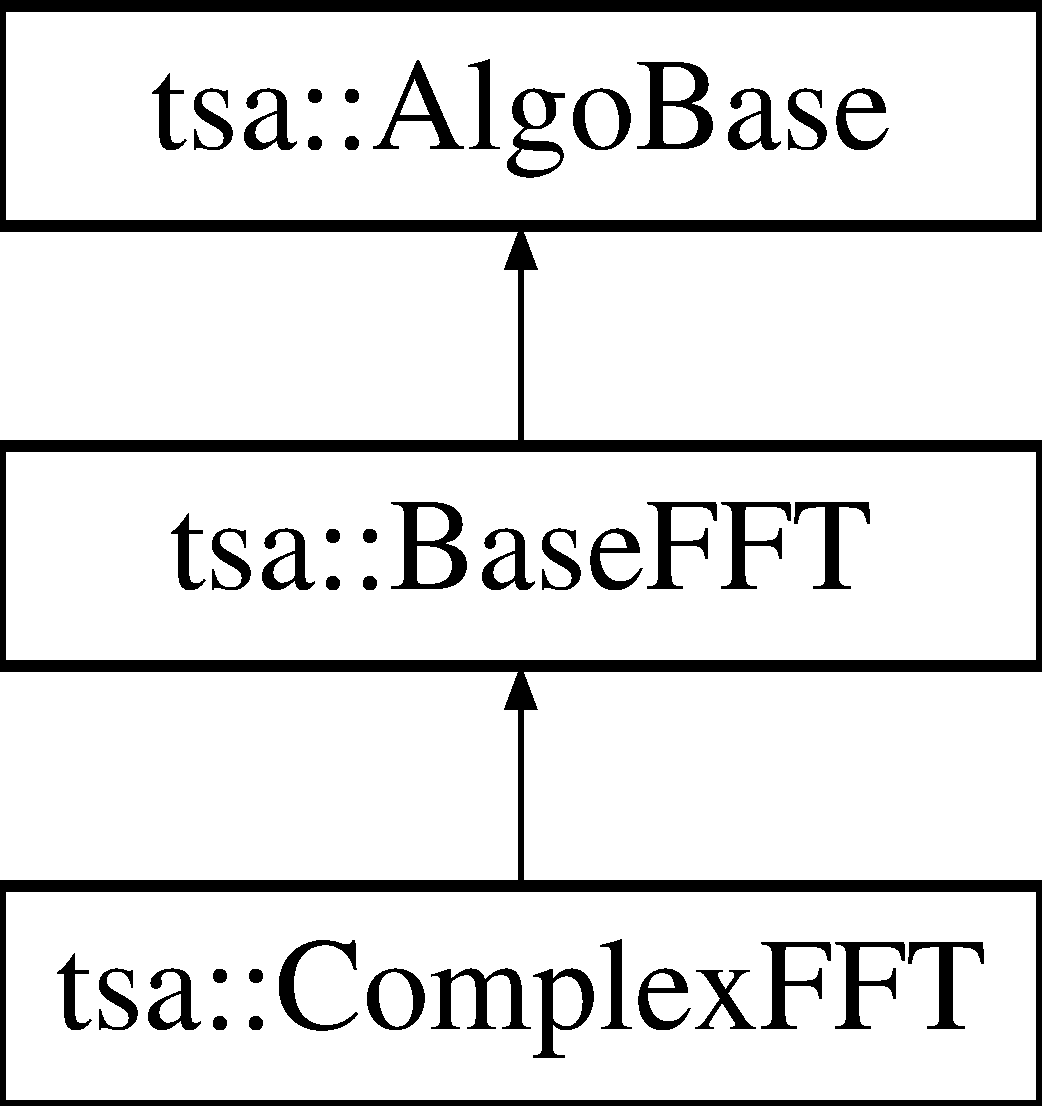
\includegraphics[height=3.000000cm]{classtsa_1_1_complex_f_f_t}
\end{center}
\end{figure}
\subsection*{Public Types}
\begin{DoxyCompactItemize}
\item 
enum \hyperlink{classtsa_1_1_complex_f_f_t_a4e90a372fa0610f957f2c683335aa766}{Transform\+Sign} \{ \hyperlink{classtsa_1_1_complex_f_f_t_a4e90a372fa0610f957f2c683335aa766a907b249808a0c1affb86572baa34510f}{F\+O\+R\+W\+A\+RD}, 
\hyperlink{classtsa_1_1_complex_f_f_t_a4e90a372fa0610f957f2c683335aa766ab056de3bb0b051b60f40de6cb7a560de}{B\+A\+C\+K\+W\+A\+RD}
 \}
\end{DoxyCompactItemize}
\subsection*{Public Member Functions}
\begin{DoxyCompactItemize}
\item 
\hyperlink{classtsa_1_1_complex_f_f_t_af51dac1a455d6e943de87f1b0cf4d3d7}{Complex\+F\+FT} (int size=0, enum \hyperlink{classtsa_1_1_complex_f_f_t_a4e90a372fa0610f957f2c683335aa766}{Transform\+Sign} s=\hyperlink{classtsa_1_1_complex_f_f_t_a4e90a372fa0610f957f2c683335aa766a907b249808a0c1affb86572baa34510f}{F\+O\+R\+W\+A\+RD}, enum \hyperlink{namespacetsa_a217e07ef78939f88b22c8428ac96b1ae}{F\+F\+T\+Planning\+Mode} mode=\hyperlink{namespacetsa_a217e07ef78939f88b22c8428ac96b1aea2762be66fb6f3e4772c7f4cc162b9750}{E\+S\+T\+I\+M\+A\+TE}, bool Preserve\+Input=true)
\item 
\hyperlink{classtsa_1_1_complex_f_f_t_a917ecfc43a0499d90abee599755625d7}{Complex\+F\+FT} (const \hyperlink{classtsa_1_1_complex_f_f_t}{Complex\+F\+FT} \&from)
\item 
\hyperlink{classtsa_1_1_complex_f_f_t_a80004962963b35cad0fb581040a47c0d}{$\sim$\+Complex\+F\+FT} ()
\item 
\hyperlink{classtsa_1_1_complex_f_f_t}{Complex\+F\+FT} \& \hyperlink{classtsa_1_1_complex_f_f_t_ae644ce76d2adce323c4244f65735d987}{operator=} (const \hyperlink{classtsa_1_1_complex_f_f_t}{Complex\+F\+FT} \&from)
\end{DoxyCompactItemize}
\begin{Indent}\textbf{ Operations}\par
\begin{DoxyCompactItemize}
\item 
void \hyperlink{classtsa_1_1_complex_f_f_t_ada17028929521c35d3505010846a9ed5}{execute} (\hyperlink{namespacetsa_a86348fef1603a135fe5fba9e5f5486ee}{Cmatrix} \&in, \hyperlink{namespacetsa_a86348fef1603a135fe5fba9e5f5486ee}{Cmatrix} \&out)  throw (bad\+\_\+matrix\+\_\+size)
\item 
void \hyperlink{classtsa_1_1_complex_f_f_t_a05acda3ab3fbb2ead70421e587cdd210}{Make\+Plan} ()  throw (std\+::runtime\+\_\+error)
\end{DoxyCompactItemize}
\end{Indent}
\begin{Indent}\textbf{ Setters}\par
\begin{DoxyCompactItemize}
\item 
void \hyperlink{classtsa_1_1_complex_f_f_t_a3096e3de532f9433415426697f5002c2}{Set\+Sign} (enum \hyperlink{classtsa_1_1_complex_f_f_t_a4e90a372fa0610f957f2c683335aa766}{Transform\+Sign} s)
\end{DoxyCompactItemize}
\end{Indent}
\subsection*{Private Attributes}
\begin{DoxyCompactItemize}
\item 
int \hyperlink{classtsa_1_1_complex_f_f_t_a97a15c1129372c7abb6ba3ba864ca065}{m\+Sign}
\end{DoxyCompactItemize}
\subsection*{Additional Inherited Members}


\subsection{Detailed Description}
Multichannel complex F\+FT. 

This is the implementation of the F\+FT of a complex multichannel buffer. The transformation is simply iterated over all the channels. 

Definition at line 73 of file Complex\+F\+F\+T.\+hpp.



\subsection{Member Enumeration Documentation}
\mbox{\Hypertarget{classtsa_1_1_complex_f_f_t_a4e90a372fa0610f957f2c683335aa766}\label{classtsa_1_1_complex_f_f_t_a4e90a372fa0610f957f2c683335aa766}} 
\index{tsa\+::\+Complex\+F\+FT@{tsa\+::\+Complex\+F\+FT}!Transform\+Sign@{Transform\+Sign}}
\index{Transform\+Sign@{Transform\+Sign}!tsa\+::\+Complex\+F\+FT@{tsa\+::\+Complex\+F\+FT}}
\subsubsection{\texorpdfstring{Transform\+Sign}{TransformSign}}
{\footnotesize\ttfamily enum \hyperlink{classtsa_1_1_complex_f_f_t_a4e90a372fa0610f957f2c683335aa766}{tsa\+::\+Complex\+F\+F\+T\+::\+Transform\+Sign}}

Transform sign. See the fftw documentation. \begin{DoxyEnumFields}{Enumerator}
\raisebox{\heightof{T}}[0pt][0pt]{\index{F\+O\+R\+W\+A\+RD@{F\+O\+R\+W\+A\+RD}!tsa\+::\+Complex\+F\+FT@{tsa\+::\+Complex\+F\+FT}}\index{tsa\+::\+Complex\+F\+FT@{tsa\+::\+Complex\+F\+FT}!F\+O\+R\+W\+A\+RD@{F\+O\+R\+W\+A\+RD}}}\mbox{\Hypertarget{classtsa_1_1_complex_f_f_t_a4e90a372fa0610f957f2c683335aa766a907b249808a0c1affb86572baa34510f}\label{classtsa_1_1_complex_f_f_t_a4e90a372fa0610f957f2c683335aa766a907b249808a0c1affb86572baa34510f}} 
F\+O\+R\+W\+A\+RD&\\
\hline

\raisebox{\heightof{T}}[0pt][0pt]{\index{B\+A\+C\+K\+W\+A\+RD@{B\+A\+C\+K\+W\+A\+RD}!tsa\+::\+Complex\+F\+FT@{tsa\+::\+Complex\+F\+FT}}\index{tsa\+::\+Complex\+F\+FT@{tsa\+::\+Complex\+F\+FT}!B\+A\+C\+K\+W\+A\+RD@{B\+A\+C\+K\+W\+A\+RD}}}\mbox{\Hypertarget{classtsa_1_1_complex_f_f_t_a4e90a372fa0610f957f2c683335aa766ab056de3bb0b051b60f40de6cb7a560de}\label{classtsa_1_1_complex_f_f_t_a4e90a372fa0610f957f2c683335aa766ab056de3bb0b051b60f40de6cb7a560de}} 
B\+A\+C\+K\+W\+A\+RD&\\
\hline

\end{DoxyEnumFields}


Definition at line 80 of file Complex\+F\+F\+T.\+hpp.



\subsection{Constructor \& Destructor Documentation}
\mbox{\Hypertarget{classtsa_1_1_complex_f_f_t_af51dac1a455d6e943de87f1b0cf4d3d7}\label{classtsa_1_1_complex_f_f_t_af51dac1a455d6e943de87f1b0cf4d3d7}} 
\index{tsa\+::\+Complex\+F\+FT@{tsa\+::\+Complex\+F\+FT}!Complex\+F\+FT@{Complex\+F\+FT}}
\index{Complex\+F\+FT@{Complex\+F\+FT}!tsa\+::\+Complex\+F\+FT@{tsa\+::\+Complex\+F\+FT}}
\subsubsection{\texorpdfstring{Complex\+F\+F\+T()}{ComplexFFT()}\hspace{0.1cm}{\footnotesize\ttfamily [1/2]}}
{\footnotesize\ttfamily tsa\+::\+Complex\+F\+F\+T\+::\+Complex\+F\+FT (\begin{DoxyParamCaption}\item[{int}]{size = {\ttfamily 0},  }\item[{enum \hyperlink{classtsa_1_1_complex_f_f_t_a4e90a372fa0610f957f2c683335aa766}{Transform\+Sign}}]{s = {\ttfamily \hyperlink{classtsa_1_1_complex_f_f_t_a4e90a372fa0610f957f2c683335aa766a907b249808a0c1affb86572baa34510f}{F\+O\+R\+W\+A\+RD}},  }\item[{enum \hyperlink{namespacetsa_a217e07ef78939f88b22c8428ac96b1ae}{F\+F\+T\+Planning\+Mode}}]{mode = {\ttfamily \hyperlink{namespacetsa_a217e07ef78939f88b22c8428ac96b1aea2762be66fb6f3e4772c7f4cc162b9750}{E\+S\+T\+I\+M\+A\+TE}},  }\item[{bool}]{Preserve\+Input = {\ttfamily true} }\end{DoxyParamCaption})}

Constructor


\begin{DoxyParams}{Parameters}
{\em size} & the size of the transform \\
\hline
{\em s} & the sign of the transform \\
\hline
{\em mode} & specify the way in which plans are calculated \\
\hline
{\em Preserve\+Input} & true if the input buffer must be preserved during the transform, false otherwise \\
\hline
\end{DoxyParams}


Definition at line 7 of file Complex\+F\+F\+T.\+cpp.

\mbox{\Hypertarget{classtsa_1_1_complex_f_f_t_a917ecfc43a0499d90abee599755625d7}\label{classtsa_1_1_complex_f_f_t_a917ecfc43a0499d90abee599755625d7}} 
\index{tsa\+::\+Complex\+F\+FT@{tsa\+::\+Complex\+F\+FT}!Complex\+F\+FT@{Complex\+F\+FT}}
\index{Complex\+F\+FT@{Complex\+F\+FT}!tsa\+::\+Complex\+F\+FT@{tsa\+::\+Complex\+F\+FT}}
\subsubsection{\texorpdfstring{Complex\+F\+F\+T()}{ComplexFFT()}\hspace{0.1cm}{\footnotesize\ttfamily [2/2]}}
{\footnotesize\ttfamily tsa\+::\+Complex\+F\+F\+T\+::\+Complex\+F\+FT (\begin{DoxyParamCaption}\item[{const \hyperlink{classtsa_1_1_complex_f_f_t}{Complex\+F\+FT} \&}]{from }\end{DoxyParamCaption})}

Copy constructor


\begin{DoxyParams}{Parameters}
{\em from} & The instance that must be copied \\
\hline
\end{DoxyParams}


Definition at line 13 of file Complex\+F\+F\+T.\+cpp.

\mbox{\Hypertarget{classtsa_1_1_complex_f_f_t_a80004962963b35cad0fb581040a47c0d}\label{classtsa_1_1_complex_f_f_t_a80004962963b35cad0fb581040a47c0d}} 
\index{tsa\+::\+Complex\+F\+FT@{tsa\+::\+Complex\+F\+FT}!````~Complex\+F\+FT@{$\sim$\+Complex\+F\+FT}}
\index{````~Complex\+F\+FT@{$\sim$\+Complex\+F\+FT}!tsa\+::\+Complex\+F\+FT@{tsa\+::\+Complex\+F\+FT}}
\subsubsection{\texorpdfstring{$\sim$\+Complex\+F\+F\+T()}{~ComplexFFT()}}
{\footnotesize\ttfamily tsa\+::\+Complex\+F\+F\+T\+::$\sim$\+Complex\+F\+FT (\begin{DoxyParamCaption}{ }\end{DoxyParamCaption})}

Destructor 

Definition at line 19 of file Complex\+F\+F\+T.\+cpp.



\subsection{Member Function Documentation}
\mbox{\Hypertarget{classtsa_1_1_complex_f_f_t_ada17028929521c35d3505010846a9ed5}\label{classtsa_1_1_complex_f_f_t_ada17028929521c35d3505010846a9ed5}} 
\index{tsa\+::\+Complex\+F\+FT@{tsa\+::\+Complex\+F\+FT}!execute@{execute}}
\index{execute@{execute}!tsa\+::\+Complex\+F\+FT@{tsa\+::\+Complex\+F\+FT}}
\subsubsection{\texorpdfstring{execute()}{execute()}}
{\footnotesize\ttfamily void tsa\+::\+Complex\+F\+F\+T\+::execute (\begin{DoxyParamCaption}\item[{\hyperlink{namespacetsa_a86348fef1603a135fe5fba9e5f5486ee}{Cmatrix} \&}]{in,  }\item[{\hyperlink{namespacetsa_a86348fef1603a135fe5fba9e5f5486ee}{Cmatrix} \&}]{out }\end{DoxyParamCaption}) throw  \hyperlink{classtsa_1_1bad__matrix__size}{bad\+\_\+matrix\+\_\+size}) }

Execution of the fft of a multichannel buffer of complex double precision numbers. Input data are organized in a matrix. Each row is a different channel, and the number of data to transform is equal to the number of columns. Both the number of rows and the number of columns can change between each call to this method. If the number of rows changes nothing special will happen, if the number of cols changes the plan is reevaluated with the current flags.

\begin{DoxyPrecond}{Precondition}
The number of rows of input and output matrix must be the same. 

The number of columns of the output matrix must be equal to the number of columns of the input matrix. 
\end{DoxyPrecond}
\begin{DoxyPostcond}{Postcondition}
the input buffer is unchanged, unless \hyperlink{classtsa_1_1_base_f_f_t_a5b1e2f36dbdfe197aa6c74d1cf963f40}{Set\+Preserve\+Input} was called with a false argument 

the output buffer contain the fft of the input data
\end{DoxyPostcond}

\begin{DoxyExceptions}{Exceptions}
{\em \hyperlink{classtsa_1_1bad__matrix__size}{bad\+\_\+matrix\+\_\+size}} & the dimension of the output array is wrong\\
\hline
\end{DoxyExceptions}

\begin{DoxyParams}{Parameters}
{\em in} & reference to the input multichannel buffer \\
\hline
{\em out} & reference to the output multichannel buffer \\
\hline
\end{DoxyParams}


Definition at line 23 of file Complex\+F\+F\+T.\+cpp.

\mbox{\Hypertarget{classtsa_1_1_complex_f_f_t_a05acda3ab3fbb2ead70421e587cdd210}\label{classtsa_1_1_complex_f_f_t_a05acda3ab3fbb2ead70421e587cdd210}} 
\index{tsa\+::\+Complex\+F\+FT@{tsa\+::\+Complex\+F\+FT}!Make\+Plan@{Make\+Plan}}
\index{Make\+Plan@{Make\+Plan}!tsa\+::\+Complex\+F\+FT@{tsa\+::\+Complex\+F\+FT}}
\subsubsection{\texorpdfstring{Make\+Plan()}{MakePlan()}}
{\footnotesize\ttfamily void tsa\+::\+Complex\+F\+F\+T\+::\+Make\+Plan (\begin{DoxyParamCaption}{ }\end{DoxyParamCaption}) throw  std\+::runtime\+\_\+error) \hspace{0.3cm}{\ttfamily [virtual]}}

Make a new plan, with the current parameters. 

Implements \hyperlink{classtsa_1_1_base_f_f_t_a9af0c36413173821cac8dbdce9cfe3b4}{tsa\+::\+Base\+F\+FT}.



Definition at line 49 of file Complex\+F\+F\+T.\+cpp.

\mbox{\Hypertarget{classtsa_1_1_complex_f_f_t_ae644ce76d2adce323c4244f65735d987}\label{classtsa_1_1_complex_f_f_t_ae644ce76d2adce323c4244f65735d987}} 
\index{tsa\+::\+Complex\+F\+FT@{tsa\+::\+Complex\+F\+FT}!operator=@{operator=}}
\index{operator=@{operator=}!tsa\+::\+Complex\+F\+FT@{tsa\+::\+Complex\+F\+FT}}
\subsubsection{\texorpdfstring{operator=()}{operator=()}}
{\footnotesize\ttfamily \hyperlink{classtsa_1_1_complex_f_f_t}{Complex\+F\+FT}\& tsa\+::\+Complex\+F\+F\+T\+::operator= (\begin{DoxyParamCaption}\item[{const \hyperlink{classtsa_1_1_complex_f_f_t}{Complex\+F\+FT} \&}]{from }\end{DoxyParamCaption})}

Assignement operator


\begin{DoxyParams}{Parameters}
{\em from} & The instance to be assigned from\\
\hline
\end{DoxyParams}
\begin{DoxyReturn}{Returns}
a reference to a new object 
\end{DoxyReturn}
\mbox{\Hypertarget{classtsa_1_1_complex_f_f_t_a3096e3de532f9433415426697f5002c2}\label{classtsa_1_1_complex_f_f_t_a3096e3de532f9433415426697f5002c2}} 
\index{tsa\+::\+Complex\+F\+FT@{tsa\+::\+Complex\+F\+FT}!Set\+Sign@{Set\+Sign}}
\index{Set\+Sign@{Set\+Sign}!tsa\+::\+Complex\+F\+FT@{tsa\+::\+Complex\+F\+FT}}
\subsubsection{\texorpdfstring{Set\+Sign()}{SetSign()}}
{\footnotesize\ttfamily void tsa\+::\+Complex\+F\+F\+T\+::\+Set\+Sign (\begin{DoxyParamCaption}\item[{enum \hyperlink{classtsa_1_1_complex_f_f_t_a4e90a372fa0610f957f2c683335aa766}{Transform\+Sign}}]{s }\end{DoxyParamCaption})}

set the sign of the transform


\begin{DoxyParams}{Parameters}
{\em s} & the new sign of the transform \\
\hline
\end{DoxyParams}


Definition at line 64 of file Complex\+F\+F\+T.\+cpp.



\subsection{Member Data Documentation}
\mbox{\Hypertarget{classtsa_1_1_complex_f_f_t_a97a15c1129372c7abb6ba3ba864ca065}\label{classtsa_1_1_complex_f_f_t_a97a15c1129372c7abb6ba3ba864ca065}} 
\index{tsa\+::\+Complex\+F\+FT@{tsa\+::\+Complex\+F\+FT}!m\+Sign@{m\+Sign}}
\index{m\+Sign@{m\+Sign}!tsa\+::\+Complex\+F\+FT@{tsa\+::\+Complex\+F\+FT}}
\subsubsection{\texorpdfstring{m\+Sign}{mSign}}
{\footnotesize\ttfamily int tsa\+::\+Complex\+F\+F\+T\+::m\+Sign\hspace{0.3cm}{\ttfamily [private]}}

The sign of the transform 

Definition at line 178 of file Complex\+F\+F\+T.\+hpp.



The documentation for this class was generated from the following files\+:\begin{DoxyCompactItemize}
\item 
/home/filip/\+Ph\+D/\+W\+D\+F\+Pipe\+\_\+test/p4\+T\+S\+A/include/\hyperlink{_complex_f_f_t_8hpp}{Complex\+F\+F\+T.\+hpp}\item 
/home/filip/\+Ph\+D/\+W\+D\+F\+Pipe\+\_\+test/p4\+T\+S\+A/src/\hyperlink{_complex_f_f_t_8cpp}{Complex\+F\+F\+T.\+cpp}\end{DoxyCompactItemize}

\hypertarget{classtsa_1_1_cs2_hamming_window}{}\section{tsa\+:\+:Cs2\+Hamming\+Window Class Reference}
\label{classtsa_1_1_cs2_hamming_window}\index{tsa\+::\+Cs2\+Hamming\+Window@{tsa\+::\+Cs2\+Hamming\+Window}}


Cs2\+Hamming windowing algorithm.  




{\ttfamily \#include $<$Cs2\+Hamming\+Window.\+hpp$>$}

Inheritance diagram for tsa\+:\+:Cs2\+Hamming\+Window\+:\begin{figure}[H]
\begin{center}
\leavevmode
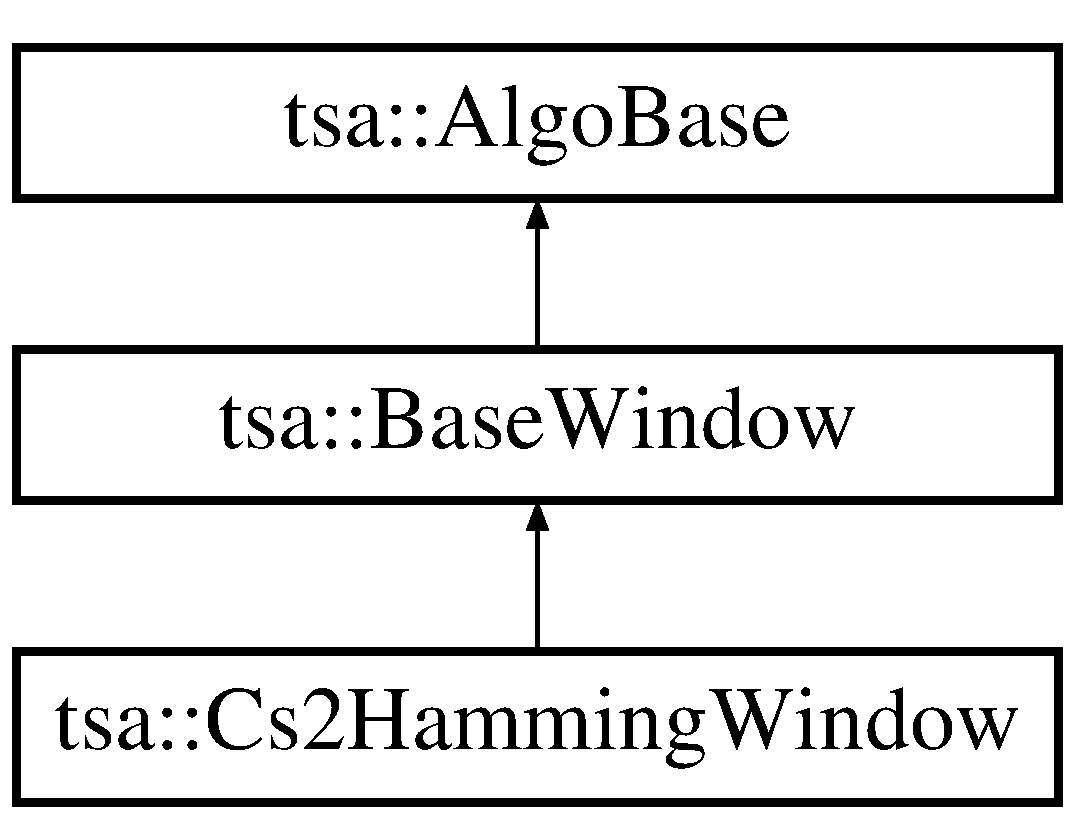
\includegraphics[height=3.000000cm]{classtsa_1_1_cs2_hamming_window}
\end{center}
\end{figure}
\subsection*{Public Member Functions}
\begin{DoxyCompactItemize}
\item 
\hyperlink{classtsa_1_1_cs2_hamming_window_a4ae0ec8d18145afbc446edef40842cf4}{Cs2\+Hamming\+Window} (int size)
\item 
\hyperlink{classtsa_1_1_cs2_hamming_window_a3f342ff907141da428f5e4255dd7763f}{Cs2\+Hamming\+Window} (int size, const std\+::string \&)
\item 
virtual \hyperlink{classtsa_1_1_cs2_hamming_window_a42a7009a9fc8e56f2508cd7d7f563fa3}{$\sim$\+Cs2\+Hamming\+Window} ()
\end{DoxyCompactItemize}
\begin{Indent}\textbf{ Operations}\par
\begin{DoxyCompactItemize}
\item 
void \hyperlink{classtsa_1_1_cs2_hamming_window_a41281794f2587c56ed52459fe0a106a2}{operator()} (\hyperlink{namespacetsa_ac599574bcc094eda25613724b8f3ca9e}{Seq\+View\+Double} \&v1)
\item 
void \hyperlink{classtsa_1_1_cs2_hamming_window_a98046f7488d9126a9041b16852491dd9}{operator()} (\hyperlink{namespacetsa_ac599574bcc094eda25613724b8f3ca9e}{Seq\+View\+Double} \&v1, \hyperlink{namespacetsa_ac599574bcc094eda25613724b8f3ca9e}{Seq\+View\+Double} \&v2)
\item 
void \hyperlink{classtsa_1_1_cs2_hamming_window_aa455906419c91055a59da8381c3a7588}{Resize} (unsigned int size)
\end{DoxyCompactItemize}
\end{Indent}
\begin{Indent}\textbf{ Getters}\par
\begin{DoxyCompactItemize}
\item 
double \hyperlink{classtsa_1_1_cs2_hamming_window_ae5b59c5596e560ad3a09c7d2633ac729}{operator()} (int i)
\end{DoxyCompactItemize}
\end{Indent}
\subsection*{Private Member Functions}
\begin{DoxyCompactItemize}
\item 
void \hyperlink{classtsa_1_1_cs2_hamming_window_a269a092db403a2bd7bb93456dc39be60}{Fill\+Window} ()
\end{DoxyCompactItemize}
\subsection*{Additional Inherited Members}


\subsection{Detailed Description}
Cs2\+Hamming windowing algorithm. 

Definition at line 73 of file Cs2\+Hamming\+Window.\+hpp.



\subsection{Constructor \& Destructor Documentation}
\mbox{\Hypertarget{classtsa_1_1_cs2_hamming_window_a4ae0ec8d18145afbc446edef40842cf4}\label{classtsa_1_1_cs2_hamming_window_a4ae0ec8d18145afbc446edef40842cf4}} 
\index{tsa\+::\+Cs2\+Hamming\+Window@{tsa\+::\+Cs2\+Hamming\+Window}!Cs2\+Hamming\+Window@{Cs2\+Hamming\+Window}}
\index{Cs2\+Hamming\+Window@{Cs2\+Hamming\+Window}!tsa\+::\+Cs2\+Hamming\+Window@{tsa\+::\+Cs2\+Hamming\+Window}}
\subsubsection{\texorpdfstring{Cs2\+Hamming\+Window()}{Cs2HammingWindow()}\hspace{0.1cm}{\footnotesize\ttfamily [1/2]}}
{\footnotesize\ttfamily tsa\+::\+Cs2\+Hamming\+Window\+::\+Cs2\+Hamming\+Window (\begin{DoxyParamCaption}\item[{int}]{size }\end{DoxyParamCaption})\hspace{0.3cm}{\ttfamily [inline]}}

Constructor


\begin{DoxyParams}{Parameters}
{\em size} & the size of the window \\
\hline
{\em cached} & true if the window must be preevaluated in a buffer \\
\hline
\end{DoxyParams}


Definition at line 82 of file Cs2\+Hamming\+Window.\+hpp.

\mbox{\Hypertarget{classtsa_1_1_cs2_hamming_window_a3f342ff907141da428f5e4255dd7763f}\label{classtsa_1_1_cs2_hamming_window_a3f342ff907141da428f5e4255dd7763f}} 
\index{tsa\+::\+Cs2\+Hamming\+Window@{tsa\+::\+Cs2\+Hamming\+Window}!Cs2\+Hamming\+Window@{Cs2\+Hamming\+Window}}
\index{Cs2\+Hamming\+Window@{Cs2\+Hamming\+Window}!tsa\+::\+Cs2\+Hamming\+Window@{tsa\+::\+Cs2\+Hamming\+Window}}
\subsubsection{\texorpdfstring{Cs2\+Hamming\+Window()}{Cs2HammingWindow()}\hspace{0.1cm}{\footnotesize\ttfamily [2/2]}}
{\footnotesize\ttfamily tsa\+::\+Cs2\+Hamming\+Window\+::\+Cs2\+Hamming\+Window (\begin{DoxyParamCaption}\item[{int}]{size,  }\item[{const std\+::string \&}]{ }\end{DoxyParamCaption})\hspace{0.3cm}{\ttfamily [inline]}}



Definition at line 88 of file Cs2\+Hamming\+Window.\+hpp.

\mbox{\Hypertarget{classtsa_1_1_cs2_hamming_window_a42a7009a9fc8e56f2508cd7d7f563fa3}\label{classtsa_1_1_cs2_hamming_window_a42a7009a9fc8e56f2508cd7d7f563fa3}} 
\index{tsa\+::\+Cs2\+Hamming\+Window@{tsa\+::\+Cs2\+Hamming\+Window}!````~Cs2\+Hamming\+Window@{$\sim$\+Cs2\+Hamming\+Window}}
\index{````~Cs2\+Hamming\+Window@{$\sim$\+Cs2\+Hamming\+Window}!tsa\+::\+Cs2\+Hamming\+Window@{tsa\+::\+Cs2\+Hamming\+Window}}
\subsubsection{\texorpdfstring{$\sim$\+Cs2\+Hamming\+Window()}{~Cs2HammingWindow()}}
{\footnotesize\ttfamily virtual tsa\+::\+Cs2\+Hamming\+Window\+::$\sim$\+Cs2\+Hamming\+Window (\begin{DoxyParamCaption}{ }\end{DoxyParamCaption})\hspace{0.3cm}{\ttfamily [inline]}, {\ttfamily [virtual]}}

Destructor 

Definition at line 97 of file Cs2\+Hamming\+Window.\+hpp.



\subsection{Member Function Documentation}
\mbox{\Hypertarget{classtsa_1_1_cs2_hamming_window_a269a092db403a2bd7bb93456dc39be60}\label{classtsa_1_1_cs2_hamming_window_a269a092db403a2bd7bb93456dc39be60}} 
\index{tsa\+::\+Cs2\+Hamming\+Window@{tsa\+::\+Cs2\+Hamming\+Window}!Fill\+Window@{Fill\+Window}}
\index{Fill\+Window@{Fill\+Window}!tsa\+::\+Cs2\+Hamming\+Window@{tsa\+::\+Cs2\+Hamming\+Window}}
\subsubsection{\texorpdfstring{Fill\+Window()}{FillWindow()}}
{\footnotesize\ttfamily void tsa\+::\+Cs2\+Hamming\+Window\+::\+Fill\+Window (\begin{DoxyParamCaption}{ }\end{DoxyParamCaption})\hspace{0.3cm}{\ttfamily [inline]}, {\ttfamily [private]}, {\ttfamily [virtual]}}

Initialize the window with the correct values, given its actual size. This is a pure virtual function, which is redefined by each window class. 

Reimplemented from \hyperlink{classtsa_1_1_base_window_aa74b29105d94caa521d308198e8e6643}{tsa\+::\+Base\+Window}.



Definition at line 208 of file Cs2\+Hamming\+Window.\+hpp.

\mbox{\Hypertarget{classtsa_1_1_cs2_hamming_window_a41281794f2587c56ed52459fe0a106a2}\label{classtsa_1_1_cs2_hamming_window_a41281794f2587c56ed52459fe0a106a2}} 
\index{tsa\+::\+Cs2\+Hamming\+Window@{tsa\+::\+Cs2\+Hamming\+Window}!operator()@{operator()}}
\index{operator()@{operator()}!tsa\+::\+Cs2\+Hamming\+Window@{tsa\+::\+Cs2\+Hamming\+Window}}
\subsubsection{\texorpdfstring{operator()()}{operator()()}\hspace{0.1cm}{\footnotesize\ttfamily [1/3]}}
{\footnotesize\ttfamily void tsa\+::\+Cs2\+Hamming\+Window\+::operator() (\begin{DoxyParamCaption}\item[{\hyperlink{namespacetsa_ac599574bcc094eda25613724b8f3ca9e}{Seq\+View\+Double} \&}]{v1 }\end{DoxyParamCaption})\hspace{0.3cm}{\ttfamily [inline]}, {\ttfamily [virtual]}}

Apply the window to a given time view.


\begin{DoxyParams}{Parameters}
{\em v1} & the time view \\
\hline
\end{DoxyParams}


Reimplemented from \hyperlink{classtsa_1_1_base_window_a05d9edb95dc01840a1b2df78dfa3a8c1}{tsa\+::\+Base\+Window}.



Definition at line 111 of file Cs2\+Hamming\+Window.\+hpp.

\mbox{\Hypertarget{classtsa_1_1_cs2_hamming_window_a98046f7488d9126a9041b16852491dd9}\label{classtsa_1_1_cs2_hamming_window_a98046f7488d9126a9041b16852491dd9}} 
\index{tsa\+::\+Cs2\+Hamming\+Window@{tsa\+::\+Cs2\+Hamming\+Window}!operator()@{operator()}}
\index{operator()@{operator()}!tsa\+::\+Cs2\+Hamming\+Window@{tsa\+::\+Cs2\+Hamming\+Window}}
\subsubsection{\texorpdfstring{operator()()}{operator()()}\hspace{0.1cm}{\footnotesize\ttfamily [2/3]}}
{\footnotesize\ttfamily void tsa\+::\+Cs2\+Hamming\+Window\+::operator() (\begin{DoxyParamCaption}\item[{\hyperlink{namespacetsa_ac599574bcc094eda25613724b8f3ca9e}{Seq\+View\+Double} \&}]{v1,  }\item[{\hyperlink{namespacetsa_ac599574bcc094eda25613724b8f3ca9e}{Seq\+View\+Double} \&}]{v2 }\end{DoxyParamCaption})\hspace{0.3cm}{\ttfamily [inline]}, {\ttfamily [virtual]}}

Apply a window to an input view and write the results on a output view.


\begin{DoxyParams}{Parameters}
{\em v1} & the input view \\
\hline
{\em v2} & the output view \\
\hline
\end{DoxyParams}


Reimplemented from \hyperlink{classtsa_1_1_base_window_afda50daa943527e09792b06e5ba69bcb}{tsa\+::\+Base\+Window}.



Definition at line 133 of file Cs2\+Hamming\+Window.\+hpp.

\mbox{\Hypertarget{classtsa_1_1_cs2_hamming_window_ae5b59c5596e560ad3a09c7d2633ac729}\label{classtsa_1_1_cs2_hamming_window_ae5b59c5596e560ad3a09c7d2633ac729}} 
\index{tsa\+::\+Cs2\+Hamming\+Window@{tsa\+::\+Cs2\+Hamming\+Window}!operator()@{operator()}}
\index{operator()@{operator()}!tsa\+::\+Cs2\+Hamming\+Window@{tsa\+::\+Cs2\+Hamming\+Window}}
\subsubsection{\texorpdfstring{operator()()}{operator()()}\hspace{0.1cm}{\footnotesize\ttfamily [3/3]}}
{\footnotesize\ttfamily double tsa\+::\+Cs2\+Hamming\+Window\+::operator() (\begin{DoxyParamCaption}\item[{int}]{i }\end{DoxyParamCaption})\hspace{0.3cm}{\ttfamily [inline]}}

Get the value of the window at a given index.

\begin{DoxyReturn}{Returns}
the value of the window at the given plage 
\end{DoxyReturn}


Definition at line 181 of file Cs2\+Hamming\+Window.\+hpp.

\mbox{\Hypertarget{classtsa_1_1_cs2_hamming_window_aa455906419c91055a59da8381c3a7588}\label{classtsa_1_1_cs2_hamming_window_aa455906419c91055a59da8381c3a7588}} 
\index{tsa\+::\+Cs2\+Hamming\+Window@{tsa\+::\+Cs2\+Hamming\+Window}!Resize@{Resize}}
\index{Resize@{Resize}!tsa\+::\+Cs2\+Hamming\+Window@{tsa\+::\+Cs2\+Hamming\+Window}}
\subsubsection{\texorpdfstring{Resize()}{Resize()}}
{\footnotesize\ttfamily void tsa\+::\+Cs2\+Hamming\+Window\+::\+Resize (\begin{DoxyParamCaption}\item[{unsigned int}]{size }\end{DoxyParamCaption})\hspace{0.3cm}{\ttfamily [inline]}, {\ttfamily [virtual]}}

Resize the window dimension.


\begin{DoxyParams}{Parameters}
{\em size} & new size for the window \\
\hline
\end{DoxyParams}


Reimplemented from \hyperlink{classtsa_1_1_base_window_a8a2a3425f2915762d50fa57dd0e04f22}{tsa\+::\+Base\+Window}.



Definition at line 162 of file Cs2\+Hamming\+Window.\+hpp.



The documentation for this class was generated from the following file\+:\begin{DoxyCompactItemize}
\item 
/home/filip/\+Ph\+D/\+W\+D\+F\+Pipe\+\_\+test/p4\+T\+S\+A/include/\hyperlink{_cs2_hamming_window_8hpp}{Cs2\+Hamming\+Window.\+hpp}\end{DoxyCompactItemize}

\hypertarget{classtsa_1_1_cs2_hann_window}{}\section{tsa\+:\+:Cs2\+Hann\+Window Class Reference}
\label{classtsa_1_1_cs2_hann_window}\index{tsa\+::\+Cs2\+Hann\+Window@{tsa\+::\+Cs2\+Hann\+Window}}


Cs2\+Hann windowing algorithm.  




{\ttfamily \#include $<$Cs2\+Hann\+Window.\+hpp$>$}

Inheritance diagram for tsa\+:\+:Cs2\+Hann\+Window\+:\begin{figure}[H]
\begin{center}
\leavevmode
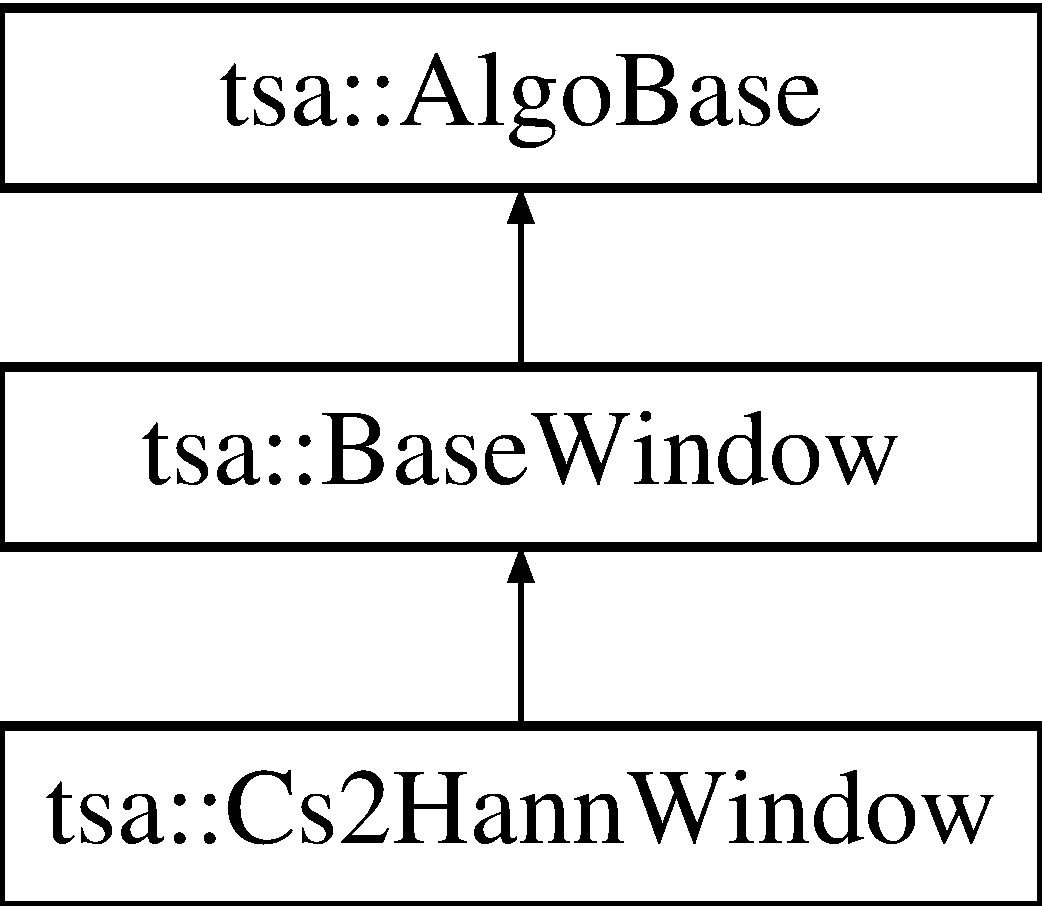
\includegraphics[height=3.000000cm]{classtsa_1_1_cs2_hann_window}
\end{center}
\end{figure}
\subsection*{Public Member Functions}
\begin{DoxyCompactItemize}
\item 
\hyperlink{classtsa_1_1_cs2_hann_window_aaa914c46b51ba07093b04a473a164699}{Cs2\+Hann\+Window} (int size)
\item 
\hyperlink{classtsa_1_1_cs2_hann_window_ac32bd6fa3481fd94c0729d6a77ca52c7}{Cs2\+Hann\+Window} (int size, const std\+::string \&)
\item 
virtual \hyperlink{classtsa_1_1_cs2_hann_window_ae46ac2cfdbfc9bef375e0cab72e379e2}{$\sim$\+Cs2\+Hann\+Window} ()
\end{DoxyCompactItemize}
\begin{Indent}\textbf{ Operations}\par
\begin{DoxyCompactItemize}
\item 
void \hyperlink{classtsa_1_1_cs2_hann_window_af896b6c2dc55a283b67c2b694926918a}{operator()} (\hyperlink{namespacetsa_ac599574bcc094eda25613724b8f3ca9e}{Seq\+View\+Double} \&v1)
\item 
void \hyperlink{classtsa_1_1_cs2_hann_window_adc0b74ee1e5173f5de7f86cf714fe47f}{operator()} (\hyperlink{namespacetsa_ac599574bcc094eda25613724b8f3ca9e}{Seq\+View\+Double} \&v1, \hyperlink{namespacetsa_ac599574bcc094eda25613724b8f3ca9e}{Seq\+View\+Double} \&v2)
\item 
void \hyperlink{classtsa_1_1_cs2_hann_window_a540187b8c32000d00d3023e8f8418264}{Resize} (unsigned int size)
\end{DoxyCompactItemize}
\end{Indent}
\subsection*{Private Member Functions}
\begin{DoxyCompactItemize}
\item 
void \hyperlink{classtsa_1_1_cs2_hann_window_a0da151916492d8ab9504ee40872131a2}{Fill\+Window} ()
\end{DoxyCompactItemize}
\subsection*{Additional Inherited Members}


\subsection{Detailed Description}
Cs2\+Hann windowing algorithm. 

Definition at line 73 of file Cs2\+Hann\+Window.\+hpp.



\subsection{Constructor \& Destructor Documentation}
\mbox{\Hypertarget{classtsa_1_1_cs2_hann_window_aaa914c46b51ba07093b04a473a164699}\label{classtsa_1_1_cs2_hann_window_aaa914c46b51ba07093b04a473a164699}} 
\index{tsa\+::\+Cs2\+Hann\+Window@{tsa\+::\+Cs2\+Hann\+Window}!Cs2\+Hann\+Window@{Cs2\+Hann\+Window}}
\index{Cs2\+Hann\+Window@{Cs2\+Hann\+Window}!tsa\+::\+Cs2\+Hann\+Window@{tsa\+::\+Cs2\+Hann\+Window}}
\subsubsection{\texorpdfstring{Cs2\+Hann\+Window()}{Cs2HannWindow()}\hspace{0.1cm}{\footnotesize\ttfamily [1/2]}}
{\footnotesize\ttfamily tsa\+::\+Cs2\+Hann\+Window\+::\+Cs2\+Hann\+Window (\begin{DoxyParamCaption}\item[{int}]{size }\end{DoxyParamCaption})\hspace{0.3cm}{\ttfamily [inline]}}

Constructor


\begin{DoxyParams}{Parameters}
{\em size} & the size of the window \\
\hline
{\em cached} & true if the window must be preevaluated in a buffer \\
\hline
\end{DoxyParams}


Definition at line 82 of file Cs2\+Hann\+Window.\+hpp.

\mbox{\Hypertarget{classtsa_1_1_cs2_hann_window_ac32bd6fa3481fd94c0729d6a77ca52c7}\label{classtsa_1_1_cs2_hann_window_ac32bd6fa3481fd94c0729d6a77ca52c7}} 
\index{tsa\+::\+Cs2\+Hann\+Window@{tsa\+::\+Cs2\+Hann\+Window}!Cs2\+Hann\+Window@{Cs2\+Hann\+Window}}
\index{Cs2\+Hann\+Window@{Cs2\+Hann\+Window}!tsa\+::\+Cs2\+Hann\+Window@{tsa\+::\+Cs2\+Hann\+Window}}
\subsubsection{\texorpdfstring{Cs2\+Hann\+Window()}{Cs2HannWindow()}\hspace{0.1cm}{\footnotesize\ttfamily [2/2]}}
{\footnotesize\ttfamily tsa\+::\+Cs2\+Hann\+Window\+::\+Cs2\+Hann\+Window (\begin{DoxyParamCaption}\item[{int}]{size,  }\item[{const std\+::string \&}]{ }\end{DoxyParamCaption})\hspace{0.3cm}{\ttfamily [inline]}}



Definition at line 88 of file Cs2\+Hann\+Window.\+hpp.

\mbox{\Hypertarget{classtsa_1_1_cs2_hann_window_ae46ac2cfdbfc9bef375e0cab72e379e2}\label{classtsa_1_1_cs2_hann_window_ae46ac2cfdbfc9bef375e0cab72e379e2}} 
\index{tsa\+::\+Cs2\+Hann\+Window@{tsa\+::\+Cs2\+Hann\+Window}!````~Cs2\+Hann\+Window@{$\sim$\+Cs2\+Hann\+Window}}
\index{````~Cs2\+Hann\+Window@{$\sim$\+Cs2\+Hann\+Window}!tsa\+::\+Cs2\+Hann\+Window@{tsa\+::\+Cs2\+Hann\+Window}}
\subsubsection{\texorpdfstring{$\sim$\+Cs2\+Hann\+Window()}{~Cs2HannWindow()}}
{\footnotesize\ttfamily virtual tsa\+::\+Cs2\+Hann\+Window\+::$\sim$\+Cs2\+Hann\+Window (\begin{DoxyParamCaption}{ }\end{DoxyParamCaption})\hspace{0.3cm}{\ttfamily [inline]}, {\ttfamily [virtual]}}

Destructor 

Definition at line 97 of file Cs2\+Hann\+Window.\+hpp.



\subsection{Member Function Documentation}
\mbox{\Hypertarget{classtsa_1_1_cs2_hann_window_a0da151916492d8ab9504ee40872131a2}\label{classtsa_1_1_cs2_hann_window_a0da151916492d8ab9504ee40872131a2}} 
\index{tsa\+::\+Cs2\+Hann\+Window@{tsa\+::\+Cs2\+Hann\+Window}!Fill\+Window@{Fill\+Window}}
\index{Fill\+Window@{Fill\+Window}!tsa\+::\+Cs2\+Hann\+Window@{tsa\+::\+Cs2\+Hann\+Window}}
\subsubsection{\texorpdfstring{Fill\+Window()}{FillWindow()}}
{\footnotesize\ttfamily void tsa\+::\+Cs2\+Hann\+Window\+::\+Fill\+Window (\begin{DoxyParamCaption}{ }\end{DoxyParamCaption})\hspace{0.3cm}{\ttfamily [inline]}, {\ttfamily [private]}, {\ttfamily [virtual]}}

Initialize the window with the correct values, given its actual size. This is a pure virtual function, which is redefined by each window class. 

Reimplemented from \hyperlink{classtsa_1_1_base_window_aa74b29105d94caa521d308198e8e6643}{tsa\+::\+Base\+Window}.



Definition at line 199 of file Cs2\+Hann\+Window.\+hpp.

\mbox{\Hypertarget{classtsa_1_1_cs2_hann_window_af896b6c2dc55a283b67c2b694926918a}\label{classtsa_1_1_cs2_hann_window_af896b6c2dc55a283b67c2b694926918a}} 
\index{tsa\+::\+Cs2\+Hann\+Window@{tsa\+::\+Cs2\+Hann\+Window}!operator()@{operator()}}
\index{operator()@{operator()}!tsa\+::\+Cs2\+Hann\+Window@{tsa\+::\+Cs2\+Hann\+Window}}
\subsubsection{\texorpdfstring{operator()()}{operator()()}\hspace{0.1cm}{\footnotesize\ttfamily [1/2]}}
{\footnotesize\ttfamily void tsa\+::\+Cs2\+Hann\+Window\+::operator() (\begin{DoxyParamCaption}\item[{\hyperlink{namespacetsa_ac599574bcc094eda25613724b8f3ca9e}{Seq\+View\+Double} \&}]{v1 }\end{DoxyParamCaption})\hspace{0.3cm}{\ttfamily [inline]}, {\ttfamily [virtual]}}

Apply the window to a given time view.


\begin{DoxyParams}{Parameters}
{\em v1} & the time view \\
\hline
\end{DoxyParams}


Reimplemented from \hyperlink{classtsa_1_1_base_window_a05d9edb95dc01840a1b2df78dfa3a8c1}{tsa\+::\+Base\+Window}.



Definition at line 111 of file Cs2\+Hann\+Window.\+hpp.

\mbox{\Hypertarget{classtsa_1_1_cs2_hann_window_adc0b74ee1e5173f5de7f86cf714fe47f}\label{classtsa_1_1_cs2_hann_window_adc0b74ee1e5173f5de7f86cf714fe47f}} 
\index{tsa\+::\+Cs2\+Hann\+Window@{tsa\+::\+Cs2\+Hann\+Window}!operator()@{operator()}}
\index{operator()@{operator()}!tsa\+::\+Cs2\+Hann\+Window@{tsa\+::\+Cs2\+Hann\+Window}}
\subsubsection{\texorpdfstring{operator()()}{operator()()}\hspace{0.1cm}{\footnotesize\ttfamily [2/2]}}
{\footnotesize\ttfamily void tsa\+::\+Cs2\+Hann\+Window\+::operator() (\begin{DoxyParamCaption}\item[{\hyperlink{namespacetsa_ac599574bcc094eda25613724b8f3ca9e}{Seq\+View\+Double} \&}]{v1,  }\item[{\hyperlink{namespacetsa_ac599574bcc094eda25613724b8f3ca9e}{Seq\+View\+Double} \&}]{v2 }\end{DoxyParamCaption})\hspace{0.3cm}{\ttfamily [inline]}, {\ttfamily [virtual]}}

Apply a window to an input view and write the results on a output view.


\begin{DoxyParams}{Parameters}
{\em v1} & the input view \\
\hline
{\em v2} & the output view \\
\hline
\end{DoxyParams}


Reimplemented from \hyperlink{classtsa_1_1_base_window_afda50daa943527e09792b06e5ba69bcb}{tsa\+::\+Base\+Window}.



Definition at line 133 of file Cs2\+Hann\+Window.\+hpp.

\mbox{\Hypertarget{classtsa_1_1_cs2_hann_window_a540187b8c32000d00d3023e8f8418264}\label{classtsa_1_1_cs2_hann_window_a540187b8c32000d00d3023e8f8418264}} 
\index{tsa\+::\+Cs2\+Hann\+Window@{tsa\+::\+Cs2\+Hann\+Window}!Resize@{Resize}}
\index{Resize@{Resize}!tsa\+::\+Cs2\+Hann\+Window@{tsa\+::\+Cs2\+Hann\+Window}}
\subsubsection{\texorpdfstring{Resize()}{Resize()}}
{\footnotesize\ttfamily void tsa\+::\+Cs2\+Hann\+Window\+::\+Resize (\begin{DoxyParamCaption}\item[{unsigned int}]{size }\end{DoxyParamCaption})\hspace{0.3cm}{\ttfamily [inline]}, {\ttfamily [virtual]}}

Resize the window dimension.


\begin{DoxyParams}{Parameters}
{\em size} & new size for the window \\
\hline
\end{DoxyParams}


Reimplemented from \hyperlink{classtsa_1_1_base_window_a8a2a3425f2915762d50fa57dd0e04f22}{tsa\+::\+Base\+Window}.



Definition at line 161 of file Cs2\+Hann\+Window.\+hpp.



The documentation for this class was generated from the following file\+:\begin{DoxyCompactItemize}
\item 
/home/filip/\+Ph\+D/\+W\+D\+F\+Pipe\+\_\+test/p4\+T\+S\+A/include/\hyperlink{_cs2_hann_window_8hpp}{Cs2\+Hann\+Window.\+hpp}\end{DoxyCompactItemize}

\hypertarget{struct_function_parser_1_1_data}{}\section{Function\+Parser\+:\+:Data Struct Reference}
\label{struct_function_parser_1_1_data}\index{Function\+Parser\+::\+Data@{Function\+Parser\+::\+Data}}
\subsection*{Classes}
\begin{DoxyCompactItemize}
\item 
struct \hyperlink{struct_function_parser_1_1_data_1_1_func_ptr_data}{Func\+Ptr\+Data}
\end{DoxyCompactItemize}
\subsection*{Public Types}
\begin{DoxyCompactItemize}
\item 
typedef std\+::map$<$ std\+::string, unsigned $>$ \hyperlink{struct_function_parser_1_1_data_a02f3fbca3164d0e498312b418258ea84}{Var\+Map\+\_\+t}
\item 
typedef std\+::map$<$ std\+::string, double $>$ \hyperlink{struct_function_parser_1_1_data_a74ff90f5d1687b68363d1602ef0ccece}{Const\+Map\+\_\+t}
\end{DoxyCompactItemize}
\subsection*{Public Member Functions}
\begin{DoxyCompactItemize}
\item 
\hyperlink{struct_function_parser_1_1_data_a2f7002e4cc588de6091472be924689b0}{Data} ()
\item 
\hyperlink{struct_function_parser_1_1_data_a1091c2cf47cbd047273335f913bb2f82}{$\sim$\+Data} ()
\item 
\hyperlink{struct_function_parser_1_1_data_a680226a014211a42b2186a3dc0da0292}{Data} (const \hyperlink{struct_function_parser_1_1_data}{Data} \&)
\item 
\hyperlink{struct_function_parser_1_1_data}{Data} \& \hyperlink{struct_function_parser_1_1_data_a5de0c72e14a8dc7fd8d708dfbb013a45}{operator=} (const \hyperlink{struct_function_parser_1_1_data}{Data} \&)
\end{DoxyCompactItemize}
\subsection*{Public Attributes}
\begin{DoxyCompactItemize}
\item 
unsigned \hyperlink{struct_function_parser_1_1_data_a73a9146066451148d4ec8fe8c0ec8418}{reference\+Counter}
\item 
int \hyperlink{struct_function_parser_1_1_data_af882554224f4977d69c5593254ac210e}{var\+Amount}
\item 
bool \hyperlink{struct_function_parser_1_1_data_a2e34291302b3dfafd29d64a6aacecb1f}{use\+Degree\+Conversion}
\item 
\hyperlink{struct_function_parser_1_1_data_a02f3fbca3164d0e498312b418258ea84}{Var\+Map\+\_\+t} \hyperlink{struct_function_parser_1_1_data_ab5d416f3bb9086ea069ce85831e4cff6}{Variables}
\item 
\hyperlink{struct_function_parser_1_1_data_a74ff90f5d1687b68363d1602ef0ccece}{Const\+Map\+\_\+t} \hyperlink{struct_function_parser_1_1_data_a832899b555441fe2ce6bfaf5e0c19f6d}{Constants}
\item 
\hyperlink{struct_function_parser_1_1_data_a02f3fbca3164d0e498312b418258ea84}{Var\+Map\+\_\+t} \hyperlink{struct_function_parser_1_1_data_aca8bc3c4c9840a4ce7fc75a6fb6d0e61}{Func\+Ptr\+Names}
\item 
std\+::vector$<$ \hyperlink{struct_function_parser_1_1_data_1_1_func_ptr_data}{Func\+Ptr\+Data} $>$ \hyperlink{struct_function_parser_1_1_data_a1ba8025daa062d7eef15b95a49c4607f}{Func\+Ptrs}
\item 
\hyperlink{struct_function_parser_1_1_data_a02f3fbca3164d0e498312b418258ea84}{Var\+Map\+\_\+t} \hyperlink{struct_function_parser_1_1_data_ac552328a6854b174a7d085d9df0c8943}{Func\+Parser\+Names}
\item 
std\+::vector$<$ \hyperlink{class_function_parser}{Function\+Parser} $\ast$ $>$ \hyperlink{struct_function_parser_1_1_data_a29d036708b0524b8ff0ddd3e6248ef6f}{Func\+Parsers}
\item 
unsigned $\ast$ \hyperlink{struct_function_parser_1_1_data_a113be528db3c02713aa9887732897f8d}{Byte\+Code}
\item 
unsigned \hyperlink{struct_function_parser_1_1_data_a6037b3f5d5d8854dfd9ec15b9ac0924f}{Byte\+Code\+Size}
\item 
double $\ast$ \hyperlink{struct_function_parser_1_1_data_a5a1b2b3c4adaed1b098413547cc67ce3}{Immed}
\item 
unsigned \hyperlink{struct_function_parser_1_1_data_a6391f52f7d877cdde635f758d7e9fdbb}{Immed\+Size}
\item 
double $\ast$ \hyperlink{struct_function_parser_1_1_data_a1ba27ea1afffc0f361e4da36723caaa7}{Stack}
\item 
unsigned \hyperlink{struct_function_parser_1_1_data_afb5f715f8c45ce98b654cb169e656c8b}{Stack\+Size}
\end{DoxyCompactItemize}


\subsection{Detailed Description}


Definition at line 81 of file fparser.\+hpp.



\subsection{Member Typedef Documentation}
\mbox{\Hypertarget{struct_function_parser_1_1_data_a74ff90f5d1687b68363d1602ef0ccece}\label{struct_function_parser_1_1_data_a74ff90f5d1687b68363d1602ef0ccece}} 
\index{Function\+Parser\+::\+Data@{Function\+Parser\+::\+Data}!Const\+Map\+\_\+t@{Const\+Map\+\_\+t}}
\index{Const\+Map\+\_\+t@{Const\+Map\+\_\+t}!Function\+Parser\+::\+Data@{Function\+Parser\+::\+Data}}
\subsubsection{\texorpdfstring{Const\+Map\+\_\+t}{ConstMap\_t}}
{\footnotesize\ttfamily typedef std\+::map$<$std\+::string, double$>$ \hyperlink{struct_function_parser_1_1_data_a74ff90f5d1687b68363d1602ef0ccece}{Function\+Parser\+::\+Data\+::\+Const\+Map\+\_\+t}}



Definition at line 90 of file fparser.\+hpp.

\mbox{\Hypertarget{struct_function_parser_1_1_data_a02f3fbca3164d0e498312b418258ea84}\label{struct_function_parser_1_1_data_a02f3fbca3164d0e498312b418258ea84}} 
\index{Function\+Parser\+::\+Data@{Function\+Parser\+::\+Data}!Var\+Map\+\_\+t@{Var\+Map\+\_\+t}}
\index{Var\+Map\+\_\+t@{Var\+Map\+\_\+t}!Function\+Parser\+::\+Data@{Function\+Parser\+::\+Data}}
\subsubsection{\texorpdfstring{Var\+Map\+\_\+t}{VarMap\_t}}
{\footnotesize\ttfamily typedef std\+::map$<$std\+::string, unsigned$>$ \hyperlink{struct_function_parser_1_1_data_a02f3fbca3164d0e498312b418258ea84}{Function\+Parser\+::\+Data\+::\+Var\+Map\+\_\+t}}



Definition at line 87 of file fparser.\+hpp.



\subsection{Constructor \& Destructor Documentation}
\mbox{\Hypertarget{struct_function_parser_1_1_data_a2f7002e4cc588de6091472be924689b0}\label{struct_function_parser_1_1_data_a2f7002e4cc588de6091472be924689b0}} 
\index{Function\+Parser\+::\+Data@{Function\+Parser\+::\+Data}!Data@{Data}}
\index{Data@{Data}!Function\+Parser\+::\+Data@{Function\+Parser\+::\+Data}}
\subsubsection{\texorpdfstring{Data()}{Data()}\hspace{0.1cm}{\footnotesize\ttfamily [1/2]}}
{\footnotesize\ttfamily Function\+Parser\+::\+Data\+::\+Data (\begin{DoxyParamCaption}{ }\end{DoxyParamCaption})}



Definition at line 114 of file fparser.\+cpp.

\mbox{\Hypertarget{struct_function_parser_1_1_data_a1091c2cf47cbd047273335f913bb2f82}\label{struct_function_parser_1_1_data_a1091c2cf47cbd047273335f913bb2f82}} 
\index{Function\+Parser\+::\+Data@{Function\+Parser\+::\+Data}!````~Data@{$\sim$\+Data}}
\index{````~Data@{$\sim$\+Data}!Function\+Parser\+::\+Data@{Function\+Parser\+::\+Data}}
\subsubsection{\texorpdfstring{$\sim$\+Data()}{~Data()}}
{\footnotesize\ttfamily Function\+Parser\+::\+Data\+::$\sim$\+Data (\begin{DoxyParamCaption}{ }\end{DoxyParamCaption})}



Definition at line 121 of file fparser.\+cpp.

\mbox{\Hypertarget{struct_function_parser_1_1_data_a680226a014211a42b2186a3dc0da0292}\label{struct_function_parser_1_1_data_a680226a014211a42b2186a3dc0da0292}} 
\index{Function\+Parser\+::\+Data@{Function\+Parser\+::\+Data}!Data@{Data}}
\index{Data@{Data}!Function\+Parser\+::\+Data@{Function\+Parser\+::\+Data}}
\subsubsection{\texorpdfstring{Data()}{Data()}\hspace{0.1cm}{\footnotesize\ttfamily [2/2]}}
{\footnotesize\ttfamily Function\+Parser\+::\+Data\+::\+Data (\begin{DoxyParamCaption}\item[{const \hyperlink{struct_function_parser_1_1_data}{Data} \&}]{cpy }\end{DoxyParamCaption})}



Definition at line 138 of file fparser.\+cpp.



\subsection{Member Function Documentation}
\mbox{\Hypertarget{struct_function_parser_1_1_data_a5de0c72e14a8dc7fd8d708dfbb013a45}\label{struct_function_parser_1_1_data_a5de0c72e14a8dc7fd8d708dfbb013a45}} 
\index{Function\+Parser\+::\+Data@{Function\+Parser\+::\+Data}!operator=@{operator=}}
\index{operator=@{operator=}!Function\+Parser\+::\+Data@{Function\+Parser\+::\+Data}}
\subsubsection{\texorpdfstring{operator=()}{operator=()}}
{\footnotesize\ttfamily \hyperlink{struct_function_parser_1_1_data}{Data}\& Function\+Parser\+::\+Data\+::operator= (\begin{DoxyParamCaption}\item[{const \hyperlink{struct_function_parser_1_1_data}{Data} \&}]{ }\end{DoxyParamCaption})}



\subsection{Member Data Documentation}
\mbox{\Hypertarget{struct_function_parser_1_1_data_a113be528db3c02713aa9887732897f8d}\label{struct_function_parser_1_1_data_a113be528db3c02713aa9887732897f8d}} 
\index{Function\+Parser\+::\+Data@{Function\+Parser\+::\+Data}!Byte\+Code@{Byte\+Code}}
\index{Byte\+Code@{Byte\+Code}!Function\+Parser\+::\+Data@{Function\+Parser\+::\+Data}}
\subsubsection{\texorpdfstring{Byte\+Code}{ByteCode}}
{\footnotesize\ttfamily unsigned$\ast$ Function\+Parser\+::\+Data\+::\+Byte\+Code}



Definition at line 107 of file fparser.\+hpp.

\mbox{\Hypertarget{struct_function_parser_1_1_data_a6037b3f5d5d8854dfd9ec15b9ac0924f}\label{struct_function_parser_1_1_data_a6037b3f5d5d8854dfd9ec15b9ac0924f}} 
\index{Function\+Parser\+::\+Data@{Function\+Parser\+::\+Data}!Byte\+Code\+Size@{Byte\+Code\+Size}}
\index{Byte\+Code\+Size@{Byte\+Code\+Size}!Function\+Parser\+::\+Data@{Function\+Parser\+::\+Data}}
\subsubsection{\texorpdfstring{Byte\+Code\+Size}{ByteCodeSize}}
{\footnotesize\ttfamily unsigned Function\+Parser\+::\+Data\+::\+Byte\+Code\+Size}



Definition at line 108 of file fparser.\+hpp.

\mbox{\Hypertarget{struct_function_parser_1_1_data_a832899b555441fe2ce6bfaf5e0c19f6d}\label{struct_function_parser_1_1_data_a832899b555441fe2ce6bfaf5e0c19f6d}} 
\index{Function\+Parser\+::\+Data@{Function\+Parser\+::\+Data}!Constants@{Constants}}
\index{Constants@{Constants}!Function\+Parser\+::\+Data@{Function\+Parser\+::\+Data}}
\subsubsection{\texorpdfstring{Constants}{Constants}}
{\footnotesize\ttfamily \hyperlink{struct_function_parser_1_1_data_a74ff90f5d1687b68363d1602ef0ccece}{Const\+Map\+\_\+t} Function\+Parser\+::\+Data\+::\+Constants}



Definition at line 91 of file fparser.\+hpp.

\mbox{\Hypertarget{struct_function_parser_1_1_data_ac552328a6854b174a7d085d9df0c8943}\label{struct_function_parser_1_1_data_ac552328a6854b174a7d085d9df0c8943}} 
\index{Function\+Parser\+::\+Data@{Function\+Parser\+::\+Data}!Func\+Parser\+Names@{Func\+Parser\+Names}}
\index{Func\+Parser\+Names@{Func\+Parser\+Names}!Function\+Parser\+::\+Data@{Function\+Parser\+::\+Data}}
\subsubsection{\texorpdfstring{Func\+Parser\+Names}{FuncParserNames}}
{\footnotesize\ttfamily \hyperlink{struct_function_parser_1_1_data_a02f3fbca3164d0e498312b418258ea84}{Var\+Map\+\_\+t} Function\+Parser\+::\+Data\+::\+Func\+Parser\+Names}



Definition at line 104 of file fparser.\+hpp.

\mbox{\Hypertarget{struct_function_parser_1_1_data_a29d036708b0524b8ff0ddd3e6248ef6f}\label{struct_function_parser_1_1_data_a29d036708b0524b8ff0ddd3e6248ef6f}} 
\index{Function\+Parser\+::\+Data@{Function\+Parser\+::\+Data}!Func\+Parsers@{Func\+Parsers}}
\index{Func\+Parsers@{Func\+Parsers}!Function\+Parser\+::\+Data@{Function\+Parser\+::\+Data}}
\subsubsection{\texorpdfstring{Func\+Parsers}{FuncParsers}}
{\footnotesize\ttfamily std\+::vector$<$\hyperlink{class_function_parser}{Function\+Parser}$\ast$$>$ Function\+Parser\+::\+Data\+::\+Func\+Parsers}



Definition at line 105 of file fparser.\+hpp.

\mbox{\Hypertarget{struct_function_parser_1_1_data_aca8bc3c4c9840a4ce7fc75a6fb6d0e61}\label{struct_function_parser_1_1_data_aca8bc3c4c9840a4ce7fc75a6fb6d0e61}} 
\index{Function\+Parser\+::\+Data@{Function\+Parser\+::\+Data}!Func\+Ptr\+Names@{Func\+Ptr\+Names}}
\index{Func\+Ptr\+Names@{Func\+Ptr\+Names}!Function\+Parser\+::\+Data@{Function\+Parser\+::\+Data}}
\subsubsection{\texorpdfstring{Func\+Ptr\+Names}{FuncPtrNames}}
{\footnotesize\ttfamily \hyperlink{struct_function_parser_1_1_data_a02f3fbca3164d0e498312b418258ea84}{Var\+Map\+\_\+t} Function\+Parser\+::\+Data\+::\+Func\+Ptr\+Names}



Definition at line 93 of file fparser.\+hpp.

\mbox{\Hypertarget{struct_function_parser_1_1_data_a1ba8025daa062d7eef15b95a49c4607f}\label{struct_function_parser_1_1_data_a1ba8025daa062d7eef15b95a49c4607f}} 
\index{Function\+Parser\+::\+Data@{Function\+Parser\+::\+Data}!Func\+Ptrs@{Func\+Ptrs}}
\index{Func\+Ptrs@{Func\+Ptrs}!Function\+Parser\+::\+Data@{Function\+Parser\+::\+Data}}
\subsubsection{\texorpdfstring{Func\+Ptrs}{FuncPtrs}}
{\footnotesize\ttfamily std\+::vector$<$\hyperlink{struct_function_parser_1_1_data_1_1_func_ptr_data}{Func\+Ptr\+Data}$>$ Function\+Parser\+::\+Data\+::\+Func\+Ptrs}



Definition at line 102 of file fparser.\+hpp.

\mbox{\Hypertarget{struct_function_parser_1_1_data_a5a1b2b3c4adaed1b098413547cc67ce3}\label{struct_function_parser_1_1_data_a5a1b2b3c4adaed1b098413547cc67ce3}} 
\index{Function\+Parser\+::\+Data@{Function\+Parser\+::\+Data}!Immed@{Immed}}
\index{Immed@{Immed}!Function\+Parser\+::\+Data@{Function\+Parser\+::\+Data}}
\subsubsection{\texorpdfstring{Immed}{Immed}}
{\footnotesize\ttfamily double$\ast$ Function\+Parser\+::\+Data\+::\+Immed}



Definition at line 109 of file fparser.\+hpp.

\mbox{\Hypertarget{struct_function_parser_1_1_data_a6391f52f7d877cdde635f758d7e9fdbb}\label{struct_function_parser_1_1_data_a6391f52f7d877cdde635f758d7e9fdbb}} 
\index{Function\+Parser\+::\+Data@{Function\+Parser\+::\+Data}!Immed\+Size@{Immed\+Size}}
\index{Immed\+Size@{Immed\+Size}!Function\+Parser\+::\+Data@{Function\+Parser\+::\+Data}}
\subsubsection{\texorpdfstring{Immed\+Size}{ImmedSize}}
{\footnotesize\ttfamily unsigned Function\+Parser\+::\+Data\+::\+Immed\+Size}



Definition at line 110 of file fparser.\+hpp.

\mbox{\Hypertarget{struct_function_parser_1_1_data_a73a9146066451148d4ec8fe8c0ec8418}\label{struct_function_parser_1_1_data_a73a9146066451148d4ec8fe8c0ec8418}} 
\index{Function\+Parser\+::\+Data@{Function\+Parser\+::\+Data}!reference\+Counter@{reference\+Counter}}
\index{reference\+Counter@{reference\+Counter}!Function\+Parser\+::\+Data@{Function\+Parser\+::\+Data}}
\subsubsection{\texorpdfstring{reference\+Counter}{referenceCounter}}
{\footnotesize\ttfamily unsigned Function\+Parser\+::\+Data\+::reference\+Counter}



Definition at line 82 of file fparser.\+hpp.

\mbox{\Hypertarget{struct_function_parser_1_1_data_a1ba27ea1afffc0f361e4da36723caaa7}\label{struct_function_parser_1_1_data_a1ba27ea1afffc0f361e4da36723caaa7}} 
\index{Function\+Parser\+::\+Data@{Function\+Parser\+::\+Data}!Stack@{Stack}}
\index{Stack@{Stack}!Function\+Parser\+::\+Data@{Function\+Parser\+::\+Data}}
\subsubsection{\texorpdfstring{Stack}{Stack}}
{\footnotesize\ttfamily double$\ast$ Function\+Parser\+::\+Data\+::\+Stack}



Definition at line 111 of file fparser.\+hpp.

\mbox{\Hypertarget{struct_function_parser_1_1_data_afb5f715f8c45ce98b654cb169e656c8b}\label{struct_function_parser_1_1_data_afb5f715f8c45ce98b654cb169e656c8b}} 
\index{Function\+Parser\+::\+Data@{Function\+Parser\+::\+Data}!Stack\+Size@{Stack\+Size}}
\index{Stack\+Size@{Stack\+Size}!Function\+Parser\+::\+Data@{Function\+Parser\+::\+Data}}
\subsubsection{\texorpdfstring{Stack\+Size}{StackSize}}
{\footnotesize\ttfamily unsigned Function\+Parser\+::\+Data\+::\+Stack\+Size}



Definition at line 112 of file fparser.\+hpp.

\mbox{\Hypertarget{struct_function_parser_1_1_data_a2e34291302b3dfafd29d64a6aacecb1f}\label{struct_function_parser_1_1_data_a2e34291302b3dfafd29d64a6aacecb1f}} 
\index{Function\+Parser\+::\+Data@{Function\+Parser\+::\+Data}!use\+Degree\+Conversion@{use\+Degree\+Conversion}}
\index{use\+Degree\+Conversion@{use\+Degree\+Conversion}!Function\+Parser\+::\+Data@{Function\+Parser\+::\+Data}}
\subsubsection{\texorpdfstring{use\+Degree\+Conversion}{useDegreeConversion}}
{\footnotesize\ttfamily bool Function\+Parser\+::\+Data\+::use\+Degree\+Conversion}



Definition at line 85 of file fparser.\+hpp.

\mbox{\Hypertarget{struct_function_parser_1_1_data_af882554224f4977d69c5593254ac210e}\label{struct_function_parser_1_1_data_af882554224f4977d69c5593254ac210e}} 
\index{Function\+Parser\+::\+Data@{Function\+Parser\+::\+Data}!var\+Amount@{var\+Amount}}
\index{var\+Amount@{var\+Amount}!Function\+Parser\+::\+Data@{Function\+Parser\+::\+Data}}
\subsubsection{\texorpdfstring{var\+Amount}{varAmount}}
{\footnotesize\ttfamily int Function\+Parser\+::\+Data\+::var\+Amount}



Definition at line 84 of file fparser.\+hpp.

\mbox{\Hypertarget{struct_function_parser_1_1_data_ab5d416f3bb9086ea069ce85831e4cff6}\label{struct_function_parser_1_1_data_ab5d416f3bb9086ea069ce85831e4cff6}} 
\index{Function\+Parser\+::\+Data@{Function\+Parser\+::\+Data}!Variables@{Variables}}
\index{Variables@{Variables}!Function\+Parser\+::\+Data@{Function\+Parser\+::\+Data}}
\subsubsection{\texorpdfstring{Variables}{Variables}}
{\footnotesize\ttfamily \hyperlink{struct_function_parser_1_1_data_a02f3fbca3164d0e498312b418258ea84}{Var\+Map\+\_\+t} Function\+Parser\+::\+Data\+::\+Variables}



Definition at line 88 of file fparser.\+hpp.



The documentation for this struct was generated from the following files\+:\begin{DoxyCompactItemize}
\item 
/home/filip/\+Ph\+D/\+W\+D\+F\+Pipe\+\_\+test/p4\+T\+S\+A/include/\hyperlink{fparser_8hpp}{fparser.\+hpp}\item 
/home/filip/\+Ph\+D/\+W\+D\+F\+Pipe\+\_\+test/p4\+T\+S\+A/src/\hyperlink{fparser_8cpp}{fparser.\+cpp}\end{DoxyCompactItemize}

\hypertarget{structtsa_1_1_data_exception}{}\section{tsa\+:\+:Data\+Exception Struct Reference}
\label{structtsa_1_1_data_exception}\index{tsa\+::\+Data\+Exception@{tsa\+::\+Data\+Exception}}


{\ttfamily \#include $<$Frame\+I\+Stream.\+hpp$>$}

\subsection*{Public Types}
\begin{DoxyCompactItemize}
\item 
enum \hyperlink{structtsa_1_1_data_exception_a712f1aa505cbed35af618dd632181d18}{exception\+\_\+type} \{ \hyperlink{structtsa_1_1_data_exception_a712f1aa505cbed35af618dd632181d18a290a1df6b3d5c0756ca3bb8c12a4e25e}{data\+\_\+loss}
 \}
\end{DoxyCompactItemize}
\subsection*{Public Member Functions}
\begin{DoxyCompactItemize}
\item 
\hyperlink{structtsa_1_1_data_exception_a9f85452c8350284658dc9c8389871c19}{Data\+Exception} (double ts, double te, \hyperlink{structtsa_1_1_data_exception_a712f1aa505cbed35af618dd632181d18}{exception\+\_\+type} e)
\end{DoxyCompactItemize}
\subsection*{Public Attributes}
\begin{DoxyCompactItemize}
\item 
\hyperlink{structtsa_1_1_data_exception_a712f1aa505cbed35af618dd632181d18}{exception\+\_\+type} \hyperlink{structtsa_1_1_data_exception_aaae025849a7bf6de877817af91482a55}{Exception}
\item 
double \hyperlink{structtsa_1_1_data_exception_a421e0d69c69536dea4e49a26eb644385}{Start\+Time}
\item 
double \hyperlink{structtsa_1_1_data_exception_a38964a3999b72d3a8860f6b870eadef6}{End\+Time}
\end{DoxyCompactItemize}


\subsection{Detailed Description}
A small structure which contains informations about a data loss period. 

Definition at line 71 of file Frame\+I\+Stream.\+hpp.



\subsection{Member Enumeration Documentation}
\mbox{\Hypertarget{structtsa_1_1_data_exception_a712f1aa505cbed35af618dd632181d18}\label{structtsa_1_1_data_exception_a712f1aa505cbed35af618dd632181d18}} 
\index{tsa\+::\+Data\+Exception@{tsa\+::\+Data\+Exception}!exception\+\_\+type@{exception\+\_\+type}}
\index{exception\+\_\+type@{exception\+\_\+type}!tsa\+::\+Data\+Exception@{tsa\+::\+Data\+Exception}}
\subsubsection{\texorpdfstring{exception\+\_\+type}{exception\_type}}
{\footnotesize\ttfamily enum \hyperlink{structtsa_1_1_data_exception_a712f1aa505cbed35af618dd632181d18}{tsa\+::\+Data\+Exception\+::exception\+\_\+type}}

Type of problem. \begin{DoxyEnumFields}{Enumerator}
\raisebox{\heightof{T}}[0pt][0pt]{\index{data\+\_\+loss@{data\+\_\+loss}!tsa\+::\+Data\+Exception@{tsa\+::\+Data\+Exception}}\index{tsa\+::\+Data\+Exception@{tsa\+::\+Data\+Exception}!data\+\_\+loss@{data\+\_\+loss}}}\mbox{\Hypertarget{structtsa_1_1_data_exception_a712f1aa505cbed35af618dd632181d18a290a1df6b3d5c0756ca3bb8c12a4e25e}\label{structtsa_1_1_data_exception_a712f1aa505cbed35af618dd632181d18a290a1df6b3d5c0756ca3bb8c12a4e25e}} 
data\+\_\+loss&Data loss \\
\hline

\end{DoxyEnumFields}


Definition at line 77 of file Frame\+I\+Stream.\+hpp.



\subsection{Constructor \& Destructor Documentation}
\mbox{\Hypertarget{structtsa_1_1_data_exception_a9f85452c8350284658dc9c8389871c19}\label{structtsa_1_1_data_exception_a9f85452c8350284658dc9c8389871c19}} 
\index{tsa\+::\+Data\+Exception@{tsa\+::\+Data\+Exception}!Data\+Exception@{Data\+Exception}}
\index{Data\+Exception@{Data\+Exception}!tsa\+::\+Data\+Exception@{tsa\+::\+Data\+Exception}}
\subsubsection{\texorpdfstring{Data\+Exception()}{DataException()}}
{\footnotesize\ttfamily tsa\+::\+Data\+Exception\+::\+Data\+Exception (\begin{DoxyParamCaption}\item[{double}]{ts,  }\item[{double}]{te,  }\item[{\hyperlink{structtsa_1_1_data_exception_a712f1aa505cbed35af618dd632181d18}{exception\+\_\+type}}]{e }\end{DoxyParamCaption})\hspace{0.3cm}{\ttfamily [inline]}}

Constructor


\begin{DoxyParams}{Parameters}
{\em ts} & start of data loss (included) \\
\hline
{\em te} & end of data loss (excluded) \\
\hline
{\em e} & problem type \\
\hline
\end{DoxyParams}


Definition at line 89 of file Frame\+I\+Stream.\+hpp.



\subsection{Member Data Documentation}
\mbox{\Hypertarget{structtsa_1_1_data_exception_a38964a3999b72d3a8860f6b870eadef6}\label{structtsa_1_1_data_exception_a38964a3999b72d3a8860f6b870eadef6}} 
\index{tsa\+::\+Data\+Exception@{tsa\+::\+Data\+Exception}!End\+Time@{End\+Time}}
\index{End\+Time@{End\+Time}!tsa\+::\+Data\+Exception@{tsa\+::\+Data\+Exception}}
\subsubsection{\texorpdfstring{End\+Time}{EndTime}}
{\footnotesize\ttfamily double tsa\+::\+Data\+Exception\+::\+End\+Time}

End time of data loss (excluded) 

Definition at line 94 of file Frame\+I\+Stream.\+hpp.

\mbox{\Hypertarget{structtsa_1_1_data_exception_aaae025849a7bf6de877817af91482a55}\label{structtsa_1_1_data_exception_aaae025849a7bf6de877817af91482a55}} 
\index{tsa\+::\+Data\+Exception@{tsa\+::\+Data\+Exception}!Exception@{Exception}}
\index{Exception@{Exception}!tsa\+::\+Data\+Exception@{tsa\+::\+Data\+Exception}}
\subsubsection{\texorpdfstring{Exception}{Exception}}
{\footnotesize\ttfamily \hyperlink{structtsa_1_1_data_exception_a712f1aa505cbed35af618dd632181d18}{exception\+\_\+type} tsa\+::\+Data\+Exception\+::\+Exception}

Exception type 

Definition at line 91 of file Frame\+I\+Stream.\+hpp.

\mbox{\Hypertarget{structtsa_1_1_data_exception_a421e0d69c69536dea4e49a26eb644385}\label{structtsa_1_1_data_exception_a421e0d69c69536dea4e49a26eb644385}} 
\index{tsa\+::\+Data\+Exception@{tsa\+::\+Data\+Exception}!Start\+Time@{Start\+Time}}
\index{Start\+Time@{Start\+Time}!tsa\+::\+Data\+Exception@{tsa\+::\+Data\+Exception}}
\subsubsection{\texorpdfstring{Start\+Time}{StartTime}}
{\footnotesize\ttfamily double tsa\+::\+Data\+Exception\+::\+Start\+Time}

Start time of data loss (included) 

Definition at line 93 of file Frame\+I\+Stream.\+hpp.



The documentation for this struct was generated from the following file\+:\begin{DoxyCompactItemize}
\item 
/home/filip/\+Ph\+D/\+W\+D\+F\+Pipe\+\_\+test/p4\+T\+S\+A/include/\hyperlink{_frame_i_stream_8hpp}{Frame\+I\+Stream.\+hpp}\end{DoxyCompactItemize}

\hypertarget{classtsa_1_1_d_c_t}{}\section{tsa\+:\+:D\+CT Class Reference}
\label{classtsa_1_1_d_c_t}\index{tsa\+::\+D\+CT@{tsa\+::\+D\+CT}}


Multichannel Discrete Cosine Transform.  




{\ttfamily \#include $<$D\+C\+T.\+hpp$>$}

Inheritance diagram for tsa\+:\+:D\+CT\+:\begin{figure}[H]
\begin{center}
\leavevmode
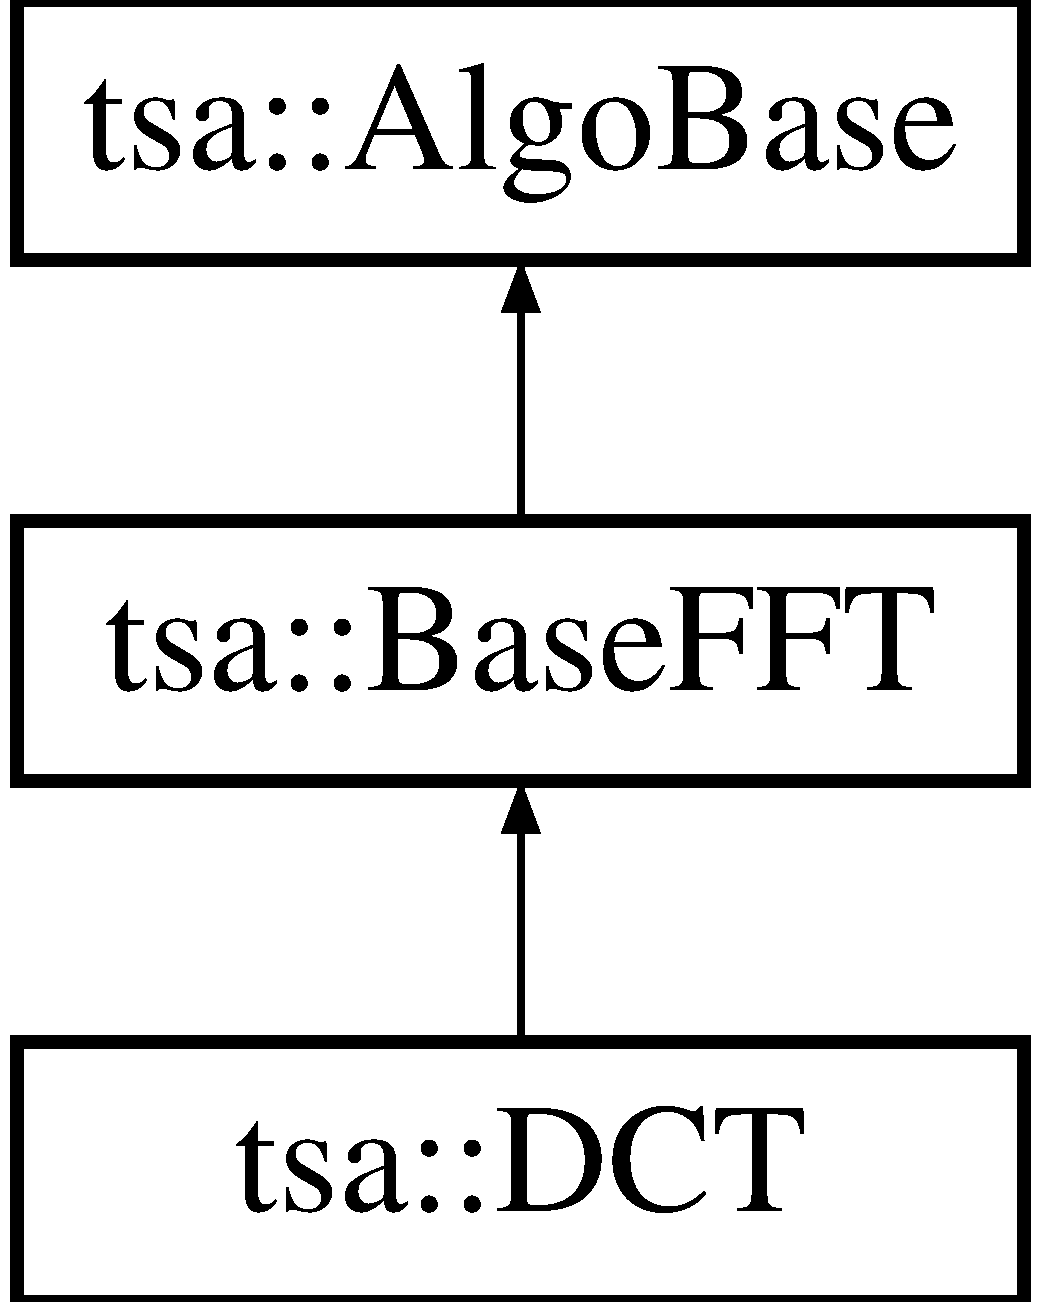
\includegraphics[height=3.000000cm]{classtsa_1_1_d_c_t}
\end{center}
\end{figure}
\subsection*{Public Member Functions}
\begin{DoxyCompactItemize}
\item 
\hyperlink{classtsa_1_1_d_c_t_af005a7dbab2f6c40e82f54a0bb55a7ec}{D\+CT} (int size=0, enum \hyperlink{namespacetsa_a217e07ef78939f88b22c8428ac96b1ae}{F\+F\+T\+Planning\+Mode} mode=\hyperlink{namespacetsa_a217e07ef78939f88b22c8428ac96b1aea2762be66fb6f3e4772c7f4cc162b9750}{E\+S\+T\+I\+M\+A\+TE}, bool Preserve\+Input=true)
\item 
\hyperlink{classtsa_1_1_d_c_t_abff7d5fe3f8f732db5963e2dfb22dfa4}{D\+CT} (const \hyperlink{classtsa_1_1_d_c_t}{D\+CT} \&from)
\item 
virtual \hyperlink{classtsa_1_1_d_c_t_a014240a8695d47e1f8191d108e88032f}{$\sim$\+D\+CT} ()
\end{DoxyCompactItemize}
\begin{Indent}\textbf{ Operations}\par
\begin{DoxyCompactItemize}
\item 
void \hyperlink{classtsa_1_1_d_c_t_a594c2f0240e0b7b4d736c498732b5bfb}{operator()} (\hyperlink{namespacetsa_ac599574bcc094eda25613724b8f3ca9e}{Seq\+View\+Double} \&in, \hyperlink{namespacetsa_ac599574bcc094eda25613724b8f3ca9e}{Seq\+View\+Double} \&out)
\item 
void \hyperlink{classtsa_1_1_d_c_t_ad659700e6288deb47359fb3797ecae21}{execute} (\hyperlink{namespacetsa_ad260cd21c1891c4ed391fe788569aba4}{Dmatrix} \&in, \hyperlink{namespacetsa_ad260cd21c1891c4ed391fe788569aba4}{Dmatrix} \&out)  throw (bad\+\_\+matrix\+\_\+size)
\item 
void \hyperlink{classtsa_1_1_d_c_t_adcdd78df5654afdc798748671a7b121d}{execute} (\hyperlink{namespacetsa_a8900fb03d849baf447a1a0efe2561fb2}{Dvector} \&in, \hyperlink{namespacetsa_a8900fb03d849baf447a1a0efe2561fb2}{Dvector} \&out)  throw (bad\+\_\+vector\+\_\+size)
\item 
void \hyperlink{classtsa_1_1_d_c_t_a2d24c07a7b3f96b16056eee1ab9bad89}{Make\+Plan} ()  throw (std\+::runtime\+\_\+error)
\end{DoxyCompactItemize}
\end{Indent}
\subsection*{Additional Inherited Members}


\subsection{Detailed Description}
Multichannel Discrete Cosine Transform. 

Definition at line 73 of file D\+C\+T.\+hpp.



\subsection{Constructor \& Destructor Documentation}
\mbox{\Hypertarget{classtsa_1_1_d_c_t_af005a7dbab2f6c40e82f54a0bb55a7ec}\label{classtsa_1_1_d_c_t_af005a7dbab2f6c40e82f54a0bb55a7ec}} 
\index{tsa\+::\+D\+CT@{tsa\+::\+D\+CT}!D\+CT@{D\+CT}}
\index{D\+CT@{D\+CT}!tsa\+::\+D\+CT@{tsa\+::\+D\+CT}}
\subsubsection{\texorpdfstring{D\+C\+T()}{DCT()}\hspace{0.1cm}{\footnotesize\ttfamily [1/2]}}
{\footnotesize\ttfamily tsa\+::\+D\+C\+T\+::\+D\+CT (\begin{DoxyParamCaption}\item[{int}]{size = {\ttfamily 0},  }\item[{enum \hyperlink{namespacetsa_a217e07ef78939f88b22c8428ac96b1ae}{F\+F\+T\+Planning\+Mode}}]{mode = {\ttfamily \hyperlink{namespacetsa_a217e07ef78939f88b22c8428ac96b1aea2762be66fb6f3e4772c7f4cc162b9750}{E\+S\+T\+I\+M\+A\+TE}},  }\item[{bool}]{Preserve\+Input = {\ttfamily true} }\end{DoxyParamCaption})}

Constructor


\begin{DoxyParams}{Parameters}
{\em size} & the size of the transform \\
\hline
{\em mode} & specify the way in which plans are calculated \\
\hline
{\em Preserve\+Input} & true if the input buffer must be preserved during the transform, false otherwise \\
\hline
\end{DoxyParams}


Definition at line 5 of file D\+C\+T.\+cpp.

\mbox{\Hypertarget{classtsa_1_1_d_c_t_abff7d5fe3f8f732db5963e2dfb22dfa4}\label{classtsa_1_1_d_c_t_abff7d5fe3f8f732db5963e2dfb22dfa4}} 
\index{tsa\+::\+D\+CT@{tsa\+::\+D\+CT}!D\+CT@{D\+CT}}
\index{D\+CT@{D\+CT}!tsa\+::\+D\+CT@{tsa\+::\+D\+CT}}
\subsubsection{\texorpdfstring{D\+C\+T()}{DCT()}\hspace{0.1cm}{\footnotesize\ttfamily [2/2]}}
{\footnotesize\ttfamily tsa\+::\+D\+C\+T\+::\+D\+CT (\begin{DoxyParamCaption}\item[{const \hyperlink{classtsa_1_1_d_c_t}{D\+CT} \&}]{from }\end{DoxyParamCaption})}

Copy constructor


\begin{DoxyParams}{Parameters}
{\em from} & The instance that must be copied \\
\hline
\end{DoxyParams}


Definition at line 11 of file D\+C\+T.\+cpp.

\mbox{\Hypertarget{classtsa_1_1_d_c_t_a014240a8695d47e1f8191d108e88032f}\label{classtsa_1_1_d_c_t_a014240a8695d47e1f8191d108e88032f}} 
\index{tsa\+::\+D\+CT@{tsa\+::\+D\+CT}!````~D\+CT@{$\sim$\+D\+CT}}
\index{````~D\+CT@{$\sim$\+D\+CT}!tsa\+::\+D\+CT@{tsa\+::\+D\+CT}}
\subsubsection{\texorpdfstring{$\sim$\+D\+C\+T()}{~DCT()}}
{\footnotesize\ttfamily tsa\+::\+D\+C\+T\+::$\sim$\+D\+CT (\begin{DoxyParamCaption}{ }\end{DoxyParamCaption})\hspace{0.3cm}{\ttfamily [virtual]}}

Destructor 

Definition at line 17 of file D\+C\+T.\+cpp.



\subsection{Member Function Documentation}
\mbox{\Hypertarget{classtsa_1_1_d_c_t_ad659700e6288deb47359fb3797ecae21}\label{classtsa_1_1_d_c_t_ad659700e6288deb47359fb3797ecae21}} 
\index{tsa\+::\+D\+CT@{tsa\+::\+D\+CT}!execute@{execute}}
\index{execute@{execute}!tsa\+::\+D\+CT@{tsa\+::\+D\+CT}}
\subsubsection{\texorpdfstring{execute()}{execute()}\hspace{0.1cm}{\footnotesize\ttfamily [1/2]}}
{\footnotesize\ttfamily void tsa\+::\+D\+C\+T\+::execute (\begin{DoxyParamCaption}\item[{\hyperlink{namespacetsa_ad260cd21c1891c4ed391fe788569aba4}{Dmatrix} \&}]{in,  }\item[{\hyperlink{namespacetsa_ad260cd21c1891c4ed391fe788569aba4}{Dmatrix} \&}]{out }\end{DoxyParamCaption}) throw  \hyperlink{classtsa_1_1bad__matrix__size}{bad\+\_\+matrix\+\_\+size}) }

Execution of the fft of a multichannel buffer of double. Input data are organized in a matrix. Each row is a different channel, and the number of data to transform is equal to the number of columns. Both the number of rows and the number of columns can change between each call to this method. If the number of rows changes nothing special will happen, if the number of cols changes the plan is reevaluated with the current flags.

\begin{DoxyPrecond}{Precondition}
The number of rows of input and output matrix must be the same. 

The columns of the output matrix must be int(n/2)+1, where n is the number of columns of the input matrix.
\end{DoxyPrecond}
\begin{DoxyPostcond}{Postcondition}
the input buffer is unchanged, unless Set\+Preserve\+Input(false) was called 

the output buffer contain the fft of the input data
\end{DoxyPostcond}

\begin{DoxyExceptions}{Exceptions}
{\em \hyperlink{classtsa_1_1bad__matrix__size}{bad\+\_\+matrix\+\_\+size}} & the size of the output matrix is wrong \\
\hline
\end{DoxyExceptions}

\begin{DoxyParams}{Parameters}
{\em in} & reference to the input multichannel buffer \\
\hline
{\em out} & reference to the output multichannel buffer \\
\hline
\end{DoxyParams}


Definition at line 42 of file D\+C\+T.\+cpp.

\mbox{\Hypertarget{classtsa_1_1_d_c_t_adcdd78df5654afdc798748671a7b121d}\label{classtsa_1_1_d_c_t_adcdd78df5654afdc798748671a7b121d}} 
\index{tsa\+::\+D\+CT@{tsa\+::\+D\+CT}!execute@{execute}}
\index{execute@{execute}!tsa\+::\+D\+CT@{tsa\+::\+D\+CT}}
\subsubsection{\texorpdfstring{execute()}{execute()}\hspace{0.1cm}{\footnotesize\ttfamily [2/2]}}
{\footnotesize\ttfamily void tsa\+::\+D\+C\+T\+::execute (\begin{DoxyParamCaption}\item[{\hyperlink{namespacetsa_a8900fb03d849baf447a1a0efe2561fb2}{Dvector} \&}]{in,  }\item[{\hyperlink{namespacetsa_a8900fb03d849baf447a1a0efe2561fb2}{Dvector} \&}]{out }\end{DoxyParamCaption}) throw  \hyperlink{classtsa_1_1bad__vector__size}{bad\+\_\+vector\+\_\+size}) }

Execution of the fft of a single channel buffer of double. If the number of the buffer changes the plan is reevaluated with the current flags.

\begin{DoxyPrecond}{Precondition}
The sized of the output vector must be int(n/2)+1, where n is the size of the input vector.
\end{DoxyPrecond}
\begin{DoxyPostcond}{Postcondition}
the input buffer is unchanged, unless Set\+Preserve\+Input(false) was called 

the output buffer contain the fft of the input data
\end{DoxyPostcond}

\begin{DoxyExceptions}{Exceptions}
{\em \hyperlink{classtsa_1_1bad__matrix__size}{bad\+\_\+matrix\+\_\+size}} & the size of the output matrix is wrong \\
\hline
\end{DoxyExceptions}

\begin{DoxyParams}{Parameters}
{\em in} & reference to the input buffer \\
\hline
{\em out} & reference to the output buffer \\
\hline
\end{DoxyParams}


Definition at line 71 of file D\+C\+T.\+cpp.

\mbox{\Hypertarget{classtsa_1_1_d_c_t_a2d24c07a7b3f96b16056eee1ab9bad89}\label{classtsa_1_1_d_c_t_a2d24c07a7b3f96b16056eee1ab9bad89}} 
\index{tsa\+::\+D\+CT@{tsa\+::\+D\+CT}!Make\+Plan@{Make\+Plan}}
\index{Make\+Plan@{Make\+Plan}!tsa\+::\+D\+CT@{tsa\+::\+D\+CT}}
\subsubsection{\texorpdfstring{Make\+Plan()}{MakePlan()}}
{\footnotesize\ttfamily void tsa\+::\+D\+C\+T\+::\+Make\+Plan (\begin{DoxyParamCaption}{ }\end{DoxyParamCaption}) throw  std\+::runtime\+\_\+error) \hspace{0.3cm}{\ttfamily [virtual]}}

Make a new plan, with the current parameters.


\begin{DoxyExceptions}{Exceptions}
{\em std\+::runtime\+\_\+error} & The new plan cannot be created \\
\hline
\end{DoxyExceptions}


Implements \hyperlink{classtsa_1_1_base_f_f_t_a9af0c36413173821cac8dbdce9cfe3b4}{tsa\+::\+Base\+F\+FT}.



Definition at line 95 of file D\+C\+T.\+cpp.

\mbox{\Hypertarget{classtsa_1_1_d_c_t_a594c2f0240e0b7b4d736c498732b5bfb}\label{classtsa_1_1_d_c_t_a594c2f0240e0b7b4d736c498732b5bfb}} 
\index{tsa\+::\+D\+CT@{tsa\+::\+D\+CT}!operator()@{operator()}}
\index{operator()@{operator()}!tsa\+::\+D\+CT@{tsa\+::\+D\+CT}}
\subsubsection{\texorpdfstring{operator()()}{operator()()}}
{\footnotesize\ttfamily void tsa\+::\+D\+C\+T\+::operator() (\begin{DoxyParamCaption}\item[{\hyperlink{namespacetsa_ac599574bcc094eda25613724b8f3ca9e}{Seq\+View\+Double} \&}]{in,  }\item[{\hyperlink{namespacetsa_ac599574bcc094eda25613724b8f3ca9e}{Seq\+View\+Double} \&}]{out }\end{DoxyParamCaption})}

Apply the transformation on the data


\begin{DoxyParams}{Parameters}
{\em in} & a reference to the buffer containing the input data \\
\hline
{\em out} & a reference to the buffer containing the input data\\
\hline
\end{DoxyParams}
\begin{DoxyReturn}{Returns}
a reference to this instance of the class 
\end{DoxyReturn}


Definition at line 21 of file D\+C\+T.\+cpp.



The documentation for this class was generated from the following files\+:\begin{DoxyCompactItemize}
\item 
/home/filip/\+Ph\+D/\+W\+D\+F\+Pipe\+\_\+test/p4\+T\+S\+A/include/\hyperlink{_d_c_t_8hpp}{D\+C\+T.\+hpp}\item 
/home/filip/\+Ph\+D/\+W\+D\+F\+Pipe\+\_\+test/p4\+T\+S\+A/src/\hyperlink{_d_c_t_8cpp}{D\+C\+T.\+cpp}\end{DoxyCompactItemize}

\hypertarget{classtsa_1_1_double_whitening}{}\section{tsa\+:\+:Double\+Whitening Class Reference}
\label{classtsa_1_1_double_whitening}\index{tsa\+::\+Double\+Whitening@{tsa\+::\+Double\+Whitening}}


Implement the double whitening filter in time domain.  




{\ttfamily \#include $<$Double\+Whitening.\+hpp$>$}

Inheritance diagram for tsa\+:\+:Double\+Whitening\+:\begin{figure}[H]
\begin{center}
\leavevmode
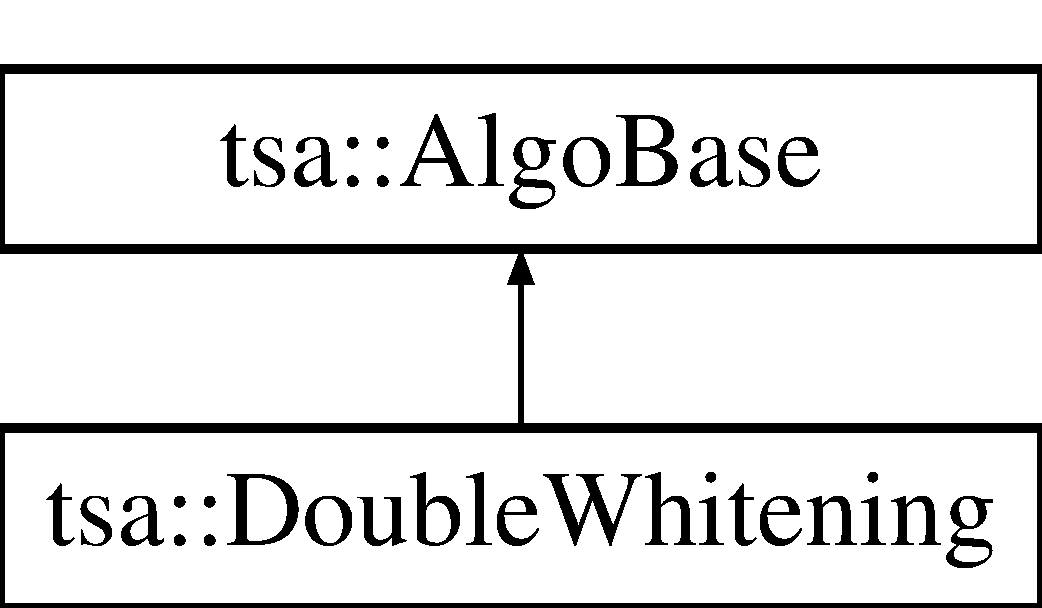
\includegraphics[height=2.000000cm]{classtsa_1_1_double_whitening}
\end{center}
\end{figure}
\subsection*{Public Member Functions}
\begin{DoxyCompactItemize}
\item 
\hyperlink{classtsa_1_1_double_whitening_ae3fdd3dfab61182230994059995ad710}{Double\+Whitening} (\hyperlink{classtsa_1_1_lattice_view}{Lattice\+View} \&LV, unsigned int Output\+Size, unsigned int Extra\+Size)
\item 
\hyperlink{classtsa_1_1_double_whitening_a58092ba19e23ed52e13c8631dd2bd011}{Double\+Whitening} (\hyperlink{namespacetsa_a8900fb03d849baf447a1a0efe2561fb2}{Dvector} \&ParcorF, \hyperlink{namespacetsa_a8900fb03d849baf447a1a0efe2561fb2}{Dvector} \&ParcorB, \hyperlink{namespacetsa_ad260cd21c1891c4ed391fe788569aba4}{Dmatrix} \&ErrF, \hyperlink{namespacetsa_ad260cd21c1891c4ed391fe788569aba4}{Dmatrix} \&ErrB, unsigned int Output\+Size, unsigned int Extra\+Size)
\item 
void \hyperlink{classtsa_1_1_double_whitening_acb49520a47e49872aa817d09b98e0b76}{init} (\hyperlink{classtsa_1_1_lattice_view}{Lattice\+View} \&LV)
\item 
virtual \hyperlink{classtsa_1_1_double_whitening_a313995cfbaec5ed83333b0b63214270b}{$\sim$\+Double\+Whitening} ()
\end{DoxyCompactItemize}
\textbf{ }\par
\begin{DoxyCompactItemize}
\item 
void \hyperlink{classtsa_1_1_double_whitening_a1e445020972445857c2aa175f3460f7e}{operator$<$$<$} (\hyperlink{namespacetsa_ac599574bcc094eda25613724b8f3ca9e}{Seq\+View\+Double} \&Data)
\item 
void \hyperlink{classtsa_1_1_double_whitening_a0dffc968e6aab0ee59cd5aa521913fce}{operator$>$$>$} (\hyperlink{namespacetsa_ac599574bcc094eda25613724b8f3ca9e}{Seq\+View\+Double} \&outdata)
\item 
\hyperlink{classtsa_1_1_double_whitening}{Double\+Whitening} \& \hyperlink{classtsa_1_1_double_whitening_a84c0175991fd9103e3783fbb8e3e1acb}{Input} (\hyperlink{namespacetsa_ac599574bcc094eda25613724b8f3ca9e}{Seq\+View\+Double} \&Data)
\item 
\hyperlink{classtsa_1_1_double_whitening}{Double\+Whitening} \& \hyperlink{classtsa_1_1_double_whitening_a7ad38eb80858187dd73cf9c86e5e9d9b}{Output} (\hyperlink{namespacetsa_ac599574bcc094eda25613724b8f3ca9e}{Seq\+View\+Double} \&outdata)
\item 
void \hyperlink{classtsa_1_1_double_whitening_a81b4fbbc957ce758982cf2b57eb46409}{Load} (const char $\ast$filename, const char $\ast$fmt=\char`\"{}txt\char`\"{})
\item 
void \hyperlink{classtsa_1_1_double_whitening_a1aa0f1d374957545ba734613f97fdfdb}{Save} (const char $\ast$filename, const char $\ast$fmt=\char`\"{}txt\char`\"{})
\item 
void \hyperlink{classtsa_1_1_double_whitening_a3c3577e865e9c733393eba9131712180}{xml\+\_\+serialize} (\hyperlink{classeternity_1_1xml__archive}{eternity\+::xml\+\_\+archive} \&xml, const char $\ast$p)
\end{DoxyCompactItemize}

\begin{Indent}\textbf{ Getters}\par
\begin{DoxyCompactItemize}
\item 
void \hyperlink{classtsa_1_1_double_whitening_abd1b553bad47599218970e1528b6c66a}{Get\+Data} (\hyperlink{namespacetsa_ad260cd21c1891c4ed391fe788569aba4}{Dmatrix} \&D\+W\+Output)
\item 
\hyperlink{namespacetsa_ad260cd21c1891c4ed391fe788569aba4}{Dmatrix} $\ast$ \hyperlink{classtsa_1_1_double_whitening_ad7fb8efabf5bc439b4d1a8aaa9ef86ea}{Get\+Whitened\+Matrix} ()
\end{DoxyCompactItemize}
\end{Indent}
\begin{Indent}\textbf{ Setters}\par
\begin{DoxyCompactItemize}
\item 
void \hyperlink{classtsa_1_1_double_whitening_a0b4972ef97afa13544eb713749d891ae}{Set\+Data} (\hyperlink{namespacetsa_ad260cd21c1891c4ed391fe788569aba4}{Dmatrix} \&Data, double scale)
\end{DoxyCompactItemize}
\end{Indent}
\subsection*{Private Attributes}
\begin{DoxyCompactItemize}
\item 
\hyperlink{classtsa_1_1_fifo_buffer}{Fifo\+Buffer} \hyperlink{classtsa_1_1_double_whitening_ad472c774f12c7ad546950187be9bafce}{m\+Buffer}
\item 
bool \hyperlink{classtsa_1_1_double_whitening_abcf4caf8a0d07a8ab19c61b73f5e36b7}{m\+First\+Call}
\item 
unsigned int \hyperlink{classtsa_1_1_double_whitening_a921503ab03e5b133a04795f04ee73b42}{m\+Output\+Size}
\item 
unsigned int \hyperlink{classtsa_1_1_double_whitening_a2cce95c06b23e6311261476052941d7c}{m\+Tot\+Size}
\item 
unsigned int \hyperlink{classtsa_1_1_double_whitening_afb79abe4e14ab46247a46de61f732db8}{m\+Order}
\item 
double \hyperlink{classtsa_1_1_double_whitening_a41231ba5d7395b08cd8a36578dc639a5}{m\+Start\+Time}
\item 
double \hyperlink{classtsa_1_1_double_whitening_a2bb0cecac07b14fbd1f05df23138f7e8}{m\+Sampling}
\item 
\hyperlink{namespacetsa_a8900fb03d849baf447a1a0efe2561fb2}{Dvector} \hyperlink{classtsa_1_1_double_whitening_a6a5ffe2b00d598c95a10913b42383361}{m\+ParcorF}
\item 
\hyperlink{namespacetsa_a8900fb03d849baf447a1a0efe2561fb2}{Dvector} \hyperlink{classtsa_1_1_double_whitening_a6b5cc8f3c501692349449d6580b739a5}{m\+ParcorB}
\item 
\hyperlink{namespacetsa_ad260cd21c1891c4ed391fe788569aba4}{Dmatrix} \hyperlink{classtsa_1_1_double_whitening_aa89217d3e82036c041f44e8f9d31951c}{m\+ErrF}
\item 
\hyperlink{namespacetsa_ad260cd21c1891c4ed391fe788569aba4}{Dmatrix} \hyperlink{classtsa_1_1_double_whitening_aeb88a0efebbd64e8b1cacaf574e62cfb}{m\+ErrB}
\item 
int \hyperlink{classtsa_1_1_double_whitening_acf877cd00f9096595ccf1bf96e07e70d}{m\+Status}
\item 
\hyperlink{namespacetsa_ad260cd21c1891c4ed391fe788569aba4}{Dmatrix} \hyperlink{classtsa_1_1_double_whitening_a210ca70e697ac431e21381905392223f}{m\+Ef}
\item 
\hyperlink{namespacetsa_ad260cd21c1891c4ed391fe788569aba4}{Dmatrix} \hyperlink{classtsa_1_1_double_whitening_a43a337d8f3320fe180dea2d4266a2a2a}{m\+Eb}
\item 
\hyperlink{namespacetsa_ad260cd21c1891c4ed391fe788569aba4}{Dmatrix} \hyperlink{classtsa_1_1_double_whitening_ae27de92c8e9e51195590dc842ce211e6}{m\+Whitened}
\end{DoxyCompactItemize}


\subsection{Detailed Description}
Implement the double whitening filter in time domain. 

A more detailed description of \hyperlink{classtsa_1_1_double_whitening}{Double\+Whitening} 

Definition at line 81 of file Double\+Whitening.\+hpp.



\subsection{Constructor \& Destructor Documentation}
\mbox{\Hypertarget{classtsa_1_1_double_whitening_ae3fdd3dfab61182230994059995ad710}\label{classtsa_1_1_double_whitening_ae3fdd3dfab61182230994059995ad710}} 
\index{tsa\+::\+Double\+Whitening@{tsa\+::\+Double\+Whitening}!Double\+Whitening@{Double\+Whitening}}
\index{Double\+Whitening@{Double\+Whitening}!tsa\+::\+Double\+Whitening@{tsa\+::\+Double\+Whitening}}
\subsubsection{\texorpdfstring{Double\+Whitening()}{DoubleWhitening()}\hspace{0.1cm}{\footnotesize\ttfamily [1/2]}}
{\footnotesize\ttfamily tsa\+::\+Double\+Whitening\+::\+Double\+Whitening (\begin{DoxyParamCaption}\item[{\hyperlink{classtsa_1_1_lattice_view}{Lattice\+View} \&}]{LV,  }\item[{unsigned int}]{Output\+Size,  }\item[{unsigned int}]{Extra\+Size }\end{DoxyParamCaption})}

Constructor 
\begin{DoxyParams}{Parameters}
{\em LV} & is the view containg the parameters for the Lattice Filter \\
\hline
\end{DoxyParams}


Definition at line 37 of file Double\+Whitening.\+cpp.

\mbox{\Hypertarget{classtsa_1_1_double_whitening_a58092ba19e23ed52e13c8631dd2bd011}\label{classtsa_1_1_double_whitening_a58092ba19e23ed52e13c8631dd2bd011}} 
\index{tsa\+::\+Double\+Whitening@{tsa\+::\+Double\+Whitening}!Double\+Whitening@{Double\+Whitening}}
\index{Double\+Whitening@{Double\+Whitening}!tsa\+::\+Double\+Whitening@{tsa\+::\+Double\+Whitening}}
\subsubsection{\texorpdfstring{Double\+Whitening()}{DoubleWhitening()}\hspace{0.1cm}{\footnotesize\ttfamily [2/2]}}
{\footnotesize\ttfamily tsa\+::\+Double\+Whitening\+::\+Double\+Whitening (\begin{DoxyParamCaption}\item[{\hyperlink{namespacetsa_a8900fb03d849baf447a1a0efe2561fb2}{Dvector} \&}]{ParcorF,  }\item[{\hyperlink{namespacetsa_a8900fb03d849baf447a1a0efe2561fb2}{Dvector} \&}]{ParcorB,  }\item[{\hyperlink{namespacetsa_ad260cd21c1891c4ed391fe788569aba4}{Dmatrix} \&}]{ErrF,  }\item[{\hyperlink{namespacetsa_ad260cd21c1891c4ed391fe788569aba4}{Dmatrix} \&}]{ErrB,  }\item[{unsigned int}]{Output\+Size,  }\item[{unsigned int}]{Extra\+Size }\end{DoxyParamCaption})}



Definition at line 19 of file Double\+Whitening.\+cpp.

\mbox{\Hypertarget{classtsa_1_1_double_whitening_a313995cfbaec5ed83333b0b63214270b}\label{classtsa_1_1_double_whitening_a313995cfbaec5ed83333b0b63214270b}} 
\index{tsa\+::\+Double\+Whitening@{tsa\+::\+Double\+Whitening}!````~Double\+Whitening@{$\sim$\+Double\+Whitening}}
\index{````~Double\+Whitening@{$\sim$\+Double\+Whitening}!tsa\+::\+Double\+Whitening@{tsa\+::\+Double\+Whitening}}
\subsubsection{\texorpdfstring{$\sim$\+Double\+Whitening()}{~DoubleWhitening()}}
{\footnotesize\ttfamily tsa\+::\+Double\+Whitening\+::$\sim$\+Double\+Whitening (\begin{DoxyParamCaption}{ }\end{DoxyParamCaption})\hspace{0.3cm}{\ttfamily [virtual]}}

Destructor 

Definition at line 63 of file Double\+Whitening.\+cpp.



\subsection{Member Function Documentation}
\mbox{\Hypertarget{classtsa_1_1_double_whitening_abd1b553bad47599218970e1528b6c66a}\label{classtsa_1_1_double_whitening_abd1b553bad47599218970e1528b6c66a}} 
\index{tsa\+::\+Double\+Whitening@{tsa\+::\+Double\+Whitening}!Get\+Data@{Get\+Data}}
\index{Get\+Data@{Get\+Data}!tsa\+::\+Double\+Whitening@{tsa\+::\+Double\+Whitening}}
\subsubsection{\texorpdfstring{Get\+Data()}{GetData()}}
{\footnotesize\ttfamily void tsa\+::\+Double\+Whitening\+::\+Get\+Data (\begin{DoxyParamCaption}\item[{\hyperlink{namespacetsa_ad260cd21c1891c4ed391fe788569aba4}{Dmatrix} \&}]{D\+W\+Output }\end{DoxyParamCaption})}



Definition at line 71 of file Double\+Whitening.\+cpp.

\mbox{\Hypertarget{classtsa_1_1_double_whitening_ad7fb8efabf5bc439b4d1a8aaa9ef86ea}\label{classtsa_1_1_double_whitening_ad7fb8efabf5bc439b4d1a8aaa9ef86ea}} 
\index{tsa\+::\+Double\+Whitening@{tsa\+::\+Double\+Whitening}!Get\+Whitened\+Matrix@{Get\+Whitened\+Matrix}}
\index{Get\+Whitened\+Matrix@{Get\+Whitened\+Matrix}!tsa\+::\+Double\+Whitening@{tsa\+::\+Double\+Whitening}}
\subsubsection{\texorpdfstring{Get\+Whitened\+Matrix()}{GetWhitenedMatrix()}}
{\footnotesize\ttfamily \hyperlink{namespacetsa_ad260cd21c1891c4ed391fe788569aba4}{Dmatrix}$\ast$ tsa\+::\+Double\+Whitening\+::\+Get\+Whitened\+Matrix (\begin{DoxyParamCaption}{ }\end{DoxyParamCaption})\hspace{0.3cm}{\ttfamily [inline]}}

\begin{DoxyReturn}{Returns}
the whitened buffer 
\end{DoxyReturn}


Definition at line 243 of file Double\+Whitening.\+hpp.

\mbox{\Hypertarget{classtsa_1_1_double_whitening_acb49520a47e49872aa817d09b98e0b76}\label{classtsa_1_1_double_whitening_acb49520a47e49872aa817d09b98e0b76}} 
\index{tsa\+::\+Double\+Whitening@{tsa\+::\+Double\+Whitening}!init@{init}}
\index{init@{init}!tsa\+::\+Double\+Whitening@{tsa\+::\+Double\+Whitening}}
\subsubsection{\texorpdfstring{init()}{init()}}
{\footnotesize\ttfamily void tsa\+::\+Double\+Whitening\+::init (\begin{DoxyParamCaption}\item[{\hyperlink{classtsa_1_1_lattice_view}{Lattice\+View} \&}]{LV }\end{DoxyParamCaption})}



Definition at line 54 of file Double\+Whitening.\+cpp.

\mbox{\Hypertarget{classtsa_1_1_double_whitening_a84c0175991fd9103e3783fbb8e3e1acb}\label{classtsa_1_1_double_whitening_a84c0175991fd9103e3783fbb8e3e1acb}} 
\index{tsa\+::\+Double\+Whitening@{tsa\+::\+Double\+Whitening}!Input@{Input}}
\index{Input@{Input}!tsa\+::\+Double\+Whitening@{tsa\+::\+Double\+Whitening}}
\subsubsection{\texorpdfstring{Input()}{Input()}}
{\footnotesize\ttfamily \hyperlink{classtsa_1_1_double_whitening}{Double\+Whitening} \& tsa\+::\+Double\+Whitening\+::\+Input (\begin{DoxyParamCaption}\item[{\hyperlink{namespacetsa_ac599574bcc094eda25613724b8f3ca9e}{Seq\+View\+Double} \&}]{Data }\end{DoxyParamCaption})}



Definition at line 168 of file Double\+Whitening.\+cpp.

\mbox{\Hypertarget{classtsa_1_1_double_whitening_a81b4fbbc957ce758982cf2b57eb46409}\label{classtsa_1_1_double_whitening_a81b4fbbc957ce758982cf2b57eb46409}} 
\index{tsa\+::\+Double\+Whitening@{tsa\+::\+Double\+Whitening}!Load@{Load}}
\index{Load@{Load}!tsa\+::\+Double\+Whitening@{tsa\+::\+Double\+Whitening}}
\subsubsection{\texorpdfstring{Load()}{Load()}}
{\footnotesize\ttfamily void tsa\+::\+Double\+Whitening\+::\+Load (\begin{DoxyParamCaption}\item[{const char $\ast$}]{filename,  }\item[{const char $\ast$}]{fmt = {\ttfamily \char`\"{}txt\char`\"{}} }\end{DoxyParamCaption})\hspace{0.3cm}{\ttfamily [inline]}}



Definition at line 141 of file Double\+Whitening.\+hpp.

\mbox{\Hypertarget{classtsa_1_1_double_whitening_a1e445020972445857c2aa175f3460f7e}\label{classtsa_1_1_double_whitening_a1e445020972445857c2aa175f3460f7e}} 
\index{tsa\+::\+Double\+Whitening@{tsa\+::\+Double\+Whitening}!operator$<$$<$@{operator$<$$<$}}
\index{operator$<$$<$@{operator$<$$<$}!tsa\+::\+Double\+Whitening@{tsa\+::\+Double\+Whitening}}
\subsubsection{\texorpdfstring{operator$<$$<$()}{operator<<()}}
{\footnotesize\ttfamily void tsa\+::\+Double\+Whitening\+::operator$<$$<$ (\begin{DoxyParamCaption}\item[{\hyperlink{namespacetsa_ac599574bcc094eda25613724b8f3ca9e}{Seq\+View\+Double} \&}]{Data }\end{DoxyParamCaption})\hspace{0.3cm}{\ttfamily [inline]}}

Declaration of execute operation


\begin{DoxyParams}{Parameters}
{\em Input\+Data} & Matrix containing Time Series \\
\hline
{\em Whitened\+Data} & Matrix containing the Whitened\+Data \\
\hline
\end{DoxyParams}


Definition at line 109 of file Double\+Whitening.\+hpp.

\mbox{\Hypertarget{classtsa_1_1_double_whitening_a0dffc968e6aab0ee59cd5aa521913fce}\label{classtsa_1_1_double_whitening_a0dffc968e6aab0ee59cd5aa521913fce}} 
\index{tsa\+::\+Double\+Whitening@{tsa\+::\+Double\+Whitening}!operator$>$$>$@{operator$>$$>$}}
\index{operator$>$$>$@{operator$>$$>$}!tsa\+::\+Double\+Whitening@{tsa\+::\+Double\+Whitening}}
\subsubsection{\texorpdfstring{operator$>$$>$()}{operator>>()}}
{\footnotesize\ttfamily void tsa\+::\+Double\+Whitening\+::operator$>$$>$ (\begin{DoxyParamCaption}\item[{\hyperlink{namespacetsa_ac599574bcc094eda25613724b8f3ca9e}{Seq\+View\+Double} \&}]{outdata }\end{DoxyParamCaption})\hspace{0.3cm}{\ttfamily [inline]}}



Definition at line 126 of file Double\+Whitening.\+hpp.

\mbox{\Hypertarget{classtsa_1_1_double_whitening_a7ad38eb80858187dd73cf9c86e5e9d9b}\label{classtsa_1_1_double_whitening_a7ad38eb80858187dd73cf9c86e5e9d9b}} 
\index{tsa\+::\+Double\+Whitening@{tsa\+::\+Double\+Whitening}!Output@{Output}}
\index{Output@{Output}!tsa\+::\+Double\+Whitening@{tsa\+::\+Double\+Whitening}}
\subsubsection{\texorpdfstring{Output()}{Output()}}
{\footnotesize\ttfamily \hyperlink{classtsa_1_1_double_whitening}{Double\+Whitening} \& tsa\+::\+Double\+Whitening\+::\+Output (\begin{DoxyParamCaption}\item[{\hyperlink{namespacetsa_ac599574bcc094eda25613724b8f3ca9e}{Seq\+View\+Double} \&}]{outdata }\end{DoxyParamCaption})}



Definition at line 187 of file Double\+Whitening.\+cpp.

\mbox{\Hypertarget{classtsa_1_1_double_whitening_a1aa0f1d374957545ba734613f97fdfdb}\label{classtsa_1_1_double_whitening_a1aa0f1d374957545ba734613f97fdfdb}} 
\index{tsa\+::\+Double\+Whitening@{tsa\+::\+Double\+Whitening}!Save@{Save}}
\index{Save@{Save}!tsa\+::\+Double\+Whitening@{tsa\+::\+Double\+Whitening}}
\subsubsection{\texorpdfstring{Save()}{Save()}}
{\footnotesize\ttfamily void tsa\+::\+Double\+Whitening\+::\+Save (\begin{DoxyParamCaption}\item[{const char $\ast$}]{filename,  }\item[{const char $\ast$}]{fmt = {\ttfamily \char`\"{}txt\char`\"{}} }\end{DoxyParamCaption})\hspace{0.3cm}{\ttfamily [inline]}}



Definition at line 148 of file Double\+Whitening.\+hpp.

\mbox{\Hypertarget{classtsa_1_1_double_whitening_a0b4972ef97afa13544eb713749d891ae}\label{classtsa_1_1_double_whitening_a0b4972ef97afa13544eb713749d891ae}} 
\index{tsa\+::\+Double\+Whitening@{tsa\+::\+Double\+Whitening}!Set\+Data@{Set\+Data}}
\index{Set\+Data@{Set\+Data}!tsa\+::\+Double\+Whitening@{tsa\+::\+Double\+Whitening}}
\subsubsection{\texorpdfstring{Set\+Data()}{SetData()}}
{\footnotesize\ttfamily void tsa\+::\+Double\+Whitening\+::\+Set\+Data (\begin{DoxyParamCaption}\item[{\hyperlink{namespacetsa_ad260cd21c1891c4ed391fe788569aba4}{Dmatrix} \&}]{Data,  }\item[{double}]{scale }\end{DoxyParamCaption})}



Definition at line 67 of file Double\+Whitening.\+cpp.

\mbox{\Hypertarget{classtsa_1_1_double_whitening_a3c3577e865e9c733393eba9131712180}\label{classtsa_1_1_double_whitening_a3c3577e865e9c733393eba9131712180}} 
\index{tsa\+::\+Double\+Whitening@{tsa\+::\+Double\+Whitening}!xml\+\_\+serialize@{xml\+\_\+serialize}}
\index{xml\+\_\+serialize@{xml\+\_\+serialize}!tsa\+::\+Double\+Whitening@{tsa\+::\+Double\+Whitening}}
\subsubsection{\texorpdfstring{xml\+\_\+serialize()}{xml\_serialize()}}
{\footnotesize\ttfamily void tsa\+::\+Double\+Whitening\+::xml\+\_\+serialize (\begin{DoxyParamCaption}\item[{\hyperlink{classeternity_1_1xml__archive}{eternity\+::xml\+\_\+archive} \&}]{xml,  }\item[{const char $\ast$}]{p }\end{DoxyParamCaption})\hspace{0.3cm}{\ttfamily [inline]}}



Definition at line 155 of file Double\+Whitening.\+hpp.



\subsection{Member Data Documentation}
\mbox{\Hypertarget{classtsa_1_1_double_whitening_ad472c774f12c7ad546950187be9bafce}\label{classtsa_1_1_double_whitening_ad472c774f12c7ad546950187be9bafce}} 
\index{tsa\+::\+Double\+Whitening@{tsa\+::\+Double\+Whitening}!m\+Buffer@{m\+Buffer}}
\index{m\+Buffer@{m\+Buffer}!tsa\+::\+Double\+Whitening@{tsa\+::\+Double\+Whitening}}
\subsubsection{\texorpdfstring{m\+Buffer}{mBuffer}}
{\footnotesize\ttfamily \hyperlink{classtsa_1_1_fifo_buffer}{Fifo\+Buffer} tsa\+::\+Double\+Whitening\+::m\+Buffer\hspace{0.3cm}{\ttfamily [private]}}



Definition at line 259 of file Double\+Whitening.\+hpp.

\mbox{\Hypertarget{classtsa_1_1_double_whitening_a43a337d8f3320fe180dea2d4266a2a2a}\label{classtsa_1_1_double_whitening_a43a337d8f3320fe180dea2d4266a2a2a}} 
\index{tsa\+::\+Double\+Whitening@{tsa\+::\+Double\+Whitening}!m\+Eb@{m\+Eb}}
\index{m\+Eb@{m\+Eb}!tsa\+::\+Double\+Whitening@{tsa\+::\+Double\+Whitening}}
\subsubsection{\texorpdfstring{m\+Eb}{mEb}}
{\footnotesize\ttfamily \hyperlink{namespacetsa_ad260cd21c1891c4ed391fe788569aba4}{Dmatrix} tsa\+::\+Double\+Whitening\+::m\+Eb\hspace{0.3cm}{\ttfamily [private]}}



Definition at line 272 of file Double\+Whitening.\+hpp.

\mbox{\Hypertarget{classtsa_1_1_double_whitening_a210ca70e697ac431e21381905392223f}\label{classtsa_1_1_double_whitening_a210ca70e697ac431e21381905392223f}} 
\index{tsa\+::\+Double\+Whitening@{tsa\+::\+Double\+Whitening}!m\+Ef@{m\+Ef}}
\index{m\+Ef@{m\+Ef}!tsa\+::\+Double\+Whitening@{tsa\+::\+Double\+Whitening}}
\subsubsection{\texorpdfstring{m\+Ef}{mEf}}
{\footnotesize\ttfamily \hyperlink{namespacetsa_ad260cd21c1891c4ed391fe788569aba4}{Dmatrix} tsa\+::\+Double\+Whitening\+::m\+Ef\hspace{0.3cm}{\ttfamily [private]}}



Definition at line 271 of file Double\+Whitening.\+hpp.

\mbox{\Hypertarget{classtsa_1_1_double_whitening_aeb88a0efebbd64e8b1cacaf574e62cfb}\label{classtsa_1_1_double_whitening_aeb88a0efebbd64e8b1cacaf574e62cfb}} 
\index{tsa\+::\+Double\+Whitening@{tsa\+::\+Double\+Whitening}!m\+ErrB@{m\+ErrB}}
\index{m\+ErrB@{m\+ErrB}!tsa\+::\+Double\+Whitening@{tsa\+::\+Double\+Whitening}}
\subsubsection{\texorpdfstring{m\+ErrB}{mErrB}}
{\footnotesize\ttfamily \hyperlink{namespacetsa_ad260cd21c1891c4ed391fe788569aba4}{Dmatrix} tsa\+::\+Double\+Whitening\+::m\+ErrB\hspace{0.3cm}{\ttfamily [private]}}



Definition at line 269 of file Double\+Whitening.\+hpp.

\mbox{\Hypertarget{classtsa_1_1_double_whitening_aa89217d3e82036c041f44e8f9d31951c}\label{classtsa_1_1_double_whitening_aa89217d3e82036c041f44e8f9d31951c}} 
\index{tsa\+::\+Double\+Whitening@{tsa\+::\+Double\+Whitening}!m\+ErrF@{m\+ErrF}}
\index{m\+ErrF@{m\+ErrF}!tsa\+::\+Double\+Whitening@{tsa\+::\+Double\+Whitening}}
\subsubsection{\texorpdfstring{m\+ErrF}{mErrF}}
{\footnotesize\ttfamily \hyperlink{namespacetsa_ad260cd21c1891c4ed391fe788569aba4}{Dmatrix} tsa\+::\+Double\+Whitening\+::m\+ErrF\hspace{0.3cm}{\ttfamily [private]}}



Definition at line 268 of file Double\+Whitening.\+hpp.

\mbox{\Hypertarget{classtsa_1_1_double_whitening_abcf4caf8a0d07a8ab19c61b73f5e36b7}\label{classtsa_1_1_double_whitening_abcf4caf8a0d07a8ab19c61b73f5e36b7}} 
\index{tsa\+::\+Double\+Whitening@{tsa\+::\+Double\+Whitening}!m\+First\+Call@{m\+First\+Call}}
\index{m\+First\+Call@{m\+First\+Call}!tsa\+::\+Double\+Whitening@{tsa\+::\+Double\+Whitening}}
\subsubsection{\texorpdfstring{m\+First\+Call}{mFirstCall}}
{\footnotesize\ttfamily bool tsa\+::\+Double\+Whitening\+::m\+First\+Call\hspace{0.3cm}{\ttfamily [private]}}



Definition at line 260 of file Double\+Whitening.\+hpp.

\mbox{\Hypertarget{classtsa_1_1_double_whitening_afb79abe4e14ab46247a46de61f732db8}\label{classtsa_1_1_double_whitening_afb79abe4e14ab46247a46de61f732db8}} 
\index{tsa\+::\+Double\+Whitening@{tsa\+::\+Double\+Whitening}!m\+Order@{m\+Order}}
\index{m\+Order@{m\+Order}!tsa\+::\+Double\+Whitening@{tsa\+::\+Double\+Whitening}}
\subsubsection{\texorpdfstring{m\+Order}{mOrder}}
{\footnotesize\ttfamily unsigned int tsa\+::\+Double\+Whitening\+::m\+Order\hspace{0.3cm}{\ttfamily [private]}}



Definition at line 263 of file Double\+Whitening.\+hpp.

\mbox{\Hypertarget{classtsa_1_1_double_whitening_a921503ab03e5b133a04795f04ee73b42}\label{classtsa_1_1_double_whitening_a921503ab03e5b133a04795f04ee73b42}} 
\index{tsa\+::\+Double\+Whitening@{tsa\+::\+Double\+Whitening}!m\+Output\+Size@{m\+Output\+Size}}
\index{m\+Output\+Size@{m\+Output\+Size}!tsa\+::\+Double\+Whitening@{tsa\+::\+Double\+Whitening}}
\subsubsection{\texorpdfstring{m\+Output\+Size}{mOutputSize}}
{\footnotesize\ttfamily unsigned int tsa\+::\+Double\+Whitening\+::m\+Output\+Size\hspace{0.3cm}{\ttfamily [private]}}



Definition at line 261 of file Double\+Whitening.\+hpp.

\mbox{\Hypertarget{classtsa_1_1_double_whitening_a6b5cc8f3c501692349449d6580b739a5}\label{classtsa_1_1_double_whitening_a6b5cc8f3c501692349449d6580b739a5}} 
\index{tsa\+::\+Double\+Whitening@{tsa\+::\+Double\+Whitening}!m\+ParcorB@{m\+ParcorB}}
\index{m\+ParcorB@{m\+ParcorB}!tsa\+::\+Double\+Whitening@{tsa\+::\+Double\+Whitening}}
\subsubsection{\texorpdfstring{m\+ParcorB}{mParcorB}}
{\footnotesize\ttfamily \hyperlink{namespacetsa_a8900fb03d849baf447a1a0efe2561fb2}{Dvector} tsa\+::\+Double\+Whitening\+::m\+ParcorB\hspace{0.3cm}{\ttfamily [private]}}



Definition at line 267 of file Double\+Whitening.\+hpp.

\mbox{\Hypertarget{classtsa_1_1_double_whitening_a6a5ffe2b00d598c95a10913b42383361}\label{classtsa_1_1_double_whitening_a6a5ffe2b00d598c95a10913b42383361}} 
\index{tsa\+::\+Double\+Whitening@{tsa\+::\+Double\+Whitening}!m\+ParcorF@{m\+ParcorF}}
\index{m\+ParcorF@{m\+ParcorF}!tsa\+::\+Double\+Whitening@{tsa\+::\+Double\+Whitening}}
\subsubsection{\texorpdfstring{m\+ParcorF}{mParcorF}}
{\footnotesize\ttfamily \hyperlink{namespacetsa_a8900fb03d849baf447a1a0efe2561fb2}{Dvector} tsa\+::\+Double\+Whitening\+::m\+ParcorF\hspace{0.3cm}{\ttfamily [private]}}



Definition at line 266 of file Double\+Whitening.\+hpp.

\mbox{\Hypertarget{classtsa_1_1_double_whitening_a2bb0cecac07b14fbd1f05df23138f7e8}\label{classtsa_1_1_double_whitening_a2bb0cecac07b14fbd1f05df23138f7e8}} 
\index{tsa\+::\+Double\+Whitening@{tsa\+::\+Double\+Whitening}!m\+Sampling@{m\+Sampling}}
\index{m\+Sampling@{m\+Sampling}!tsa\+::\+Double\+Whitening@{tsa\+::\+Double\+Whitening}}
\subsubsection{\texorpdfstring{m\+Sampling}{mSampling}}
{\footnotesize\ttfamily double tsa\+::\+Double\+Whitening\+::m\+Sampling\hspace{0.3cm}{\ttfamily [private]}}



Definition at line 265 of file Double\+Whitening.\+hpp.

\mbox{\Hypertarget{classtsa_1_1_double_whitening_a41231ba5d7395b08cd8a36578dc639a5}\label{classtsa_1_1_double_whitening_a41231ba5d7395b08cd8a36578dc639a5}} 
\index{tsa\+::\+Double\+Whitening@{tsa\+::\+Double\+Whitening}!m\+Start\+Time@{m\+Start\+Time}}
\index{m\+Start\+Time@{m\+Start\+Time}!tsa\+::\+Double\+Whitening@{tsa\+::\+Double\+Whitening}}
\subsubsection{\texorpdfstring{m\+Start\+Time}{mStartTime}}
{\footnotesize\ttfamily double tsa\+::\+Double\+Whitening\+::m\+Start\+Time\hspace{0.3cm}{\ttfamily [private]}}



Definition at line 264 of file Double\+Whitening.\+hpp.

\mbox{\Hypertarget{classtsa_1_1_double_whitening_acf877cd00f9096595ccf1bf96e07e70d}\label{classtsa_1_1_double_whitening_acf877cd00f9096595ccf1bf96e07e70d}} 
\index{tsa\+::\+Double\+Whitening@{tsa\+::\+Double\+Whitening}!m\+Status@{m\+Status}}
\index{m\+Status@{m\+Status}!tsa\+::\+Double\+Whitening@{tsa\+::\+Double\+Whitening}}
\subsubsection{\texorpdfstring{m\+Status}{mStatus}}
{\footnotesize\ttfamily int tsa\+::\+Double\+Whitening\+::m\+Status\hspace{0.3cm}{\ttfamily [private]}}



Definition at line 270 of file Double\+Whitening.\+hpp.

\mbox{\Hypertarget{classtsa_1_1_double_whitening_a2cce95c06b23e6311261476052941d7c}\label{classtsa_1_1_double_whitening_a2cce95c06b23e6311261476052941d7c}} 
\index{tsa\+::\+Double\+Whitening@{tsa\+::\+Double\+Whitening}!m\+Tot\+Size@{m\+Tot\+Size}}
\index{m\+Tot\+Size@{m\+Tot\+Size}!tsa\+::\+Double\+Whitening@{tsa\+::\+Double\+Whitening}}
\subsubsection{\texorpdfstring{m\+Tot\+Size}{mTotSize}}
{\footnotesize\ttfamily unsigned int tsa\+::\+Double\+Whitening\+::m\+Tot\+Size\hspace{0.3cm}{\ttfamily [private]}}



Definition at line 262 of file Double\+Whitening.\+hpp.

\mbox{\Hypertarget{classtsa_1_1_double_whitening_ae27de92c8e9e51195590dc842ce211e6}\label{classtsa_1_1_double_whitening_ae27de92c8e9e51195590dc842ce211e6}} 
\index{tsa\+::\+Double\+Whitening@{tsa\+::\+Double\+Whitening}!m\+Whitened@{m\+Whitened}}
\index{m\+Whitened@{m\+Whitened}!tsa\+::\+Double\+Whitening@{tsa\+::\+Double\+Whitening}}
\subsubsection{\texorpdfstring{m\+Whitened}{mWhitened}}
{\footnotesize\ttfamily \hyperlink{namespacetsa_ad260cd21c1891c4ed391fe788569aba4}{Dmatrix} tsa\+::\+Double\+Whitening\+::m\+Whitened\hspace{0.3cm}{\ttfamily [private]}}



Definition at line 273 of file Double\+Whitening.\+hpp.



The documentation for this class was generated from the following files\+:\begin{DoxyCompactItemize}
\item 
/home/filip/\+Ph\+D/\+W\+D\+F\+Pipe\+\_\+test/p4\+T\+S\+A/include/\hyperlink{_double_whitening_8hpp}{Double\+Whitening.\+hpp}\item 
/home/filip/\+Ph\+D/\+W\+D\+F\+Pipe\+\_\+test/p4\+T\+S\+A/src/\hyperlink{_double_whitening_8cpp}{Double\+Whitening.\+cpp}\end{DoxyCompactItemize}

\hypertarget{classtsa_1_1_d_s_t}{}\section{tsa\+:\+:D\+ST Class Reference}
\label{classtsa_1_1_d_s_t}\index{tsa\+::\+D\+ST@{tsa\+::\+D\+ST}}


Multichannel Discrete Sine Transform.  




{\ttfamily \#include $<$D\+S\+T.\+hpp$>$}

Inheritance diagram for tsa\+:\+:D\+ST\+:\begin{figure}[H]
\begin{center}
\leavevmode
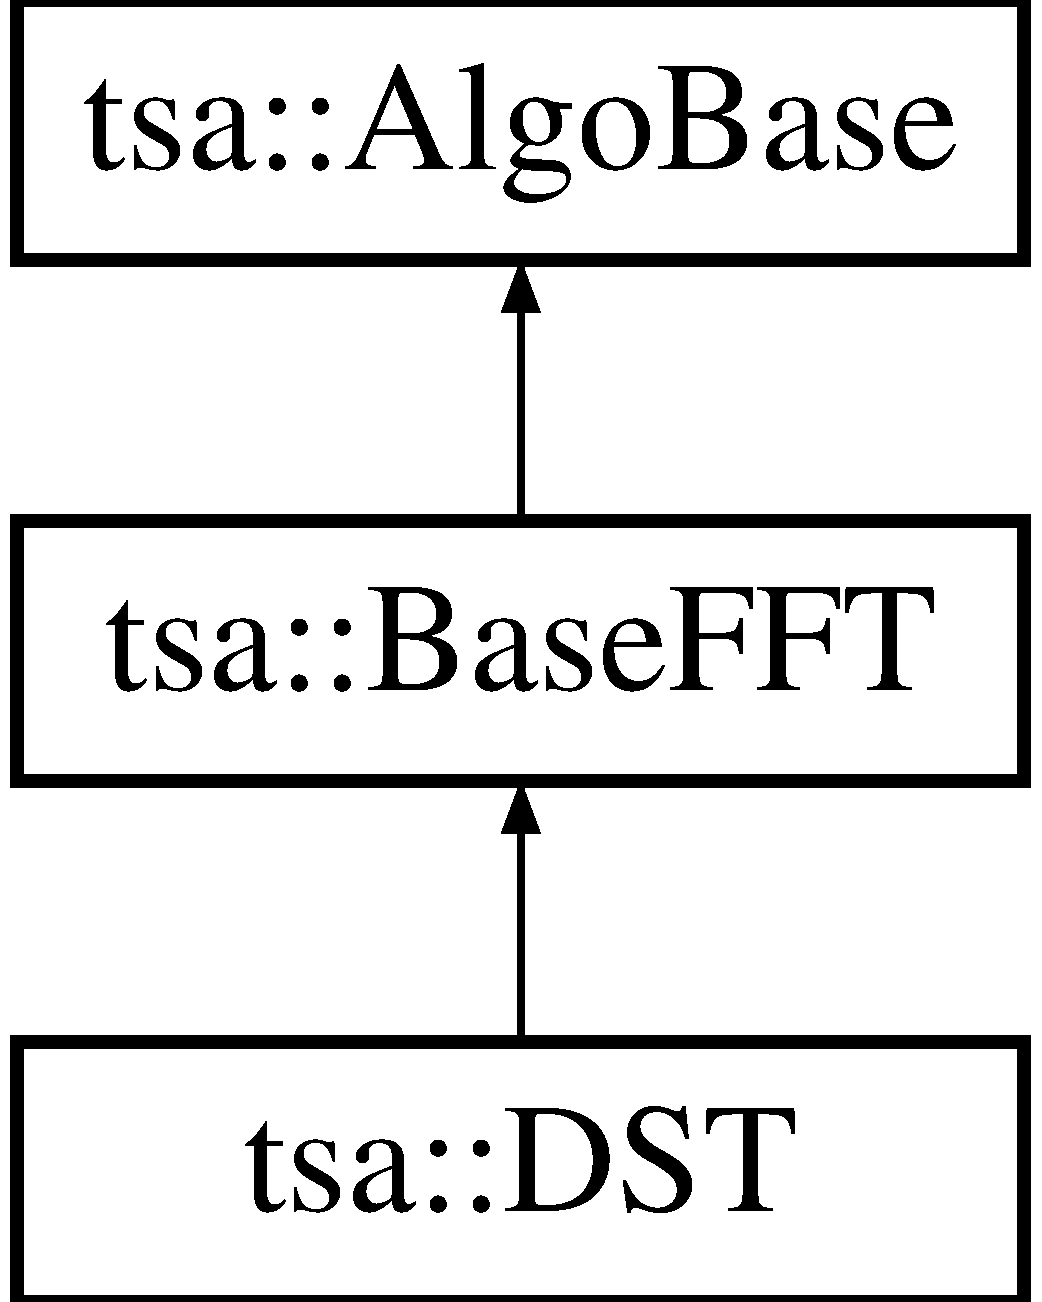
\includegraphics[height=3.000000cm]{classtsa_1_1_d_s_t}
\end{center}
\end{figure}
\subsection*{Public Member Functions}
\begin{DoxyCompactItemize}
\item 
\hyperlink{classtsa_1_1_d_s_t_a903a949ad84aaa3f5ef11e9f08a1abf9}{D\+ST} (int size=0, enum \hyperlink{namespacetsa_a217e07ef78939f88b22c8428ac96b1ae}{F\+F\+T\+Planning\+Mode} mode=\hyperlink{namespacetsa_a217e07ef78939f88b22c8428ac96b1aea2762be66fb6f3e4772c7f4cc162b9750}{E\+S\+T\+I\+M\+A\+TE}, bool Preserve\+Input=true)
\item 
\hyperlink{classtsa_1_1_d_s_t_ac7d9747deee363dbd0d20edc19d0028a}{D\+ST} (const \hyperlink{classtsa_1_1_d_s_t}{D\+ST} \&from)
\item 
virtual \hyperlink{classtsa_1_1_d_s_t_a670a8bae9d3361b5a0e0be7160fee75c}{$\sim$\+D\+ST} ()
\end{DoxyCompactItemize}
\begin{Indent}\textbf{ Operations}\par
\begin{DoxyCompactItemize}
\item 
void \hyperlink{classtsa_1_1_d_s_t_a98927f7365561b6af059465598eb3445}{operator()} (\hyperlink{namespacetsa_ac599574bcc094eda25613724b8f3ca9e}{Seq\+View\+Double} \&in, \hyperlink{namespacetsa_ac599574bcc094eda25613724b8f3ca9e}{Seq\+View\+Double} \&out)
\item 
void \hyperlink{classtsa_1_1_d_s_t_a9bb56b2c2e4b7bff93d06a065903c347}{execute} (\hyperlink{namespacetsa_ad260cd21c1891c4ed391fe788569aba4}{Dmatrix} \&in, \hyperlink{namespacetsa_ad260cd21c1891c4ed391fe788569aba4}{Dmatrix} \&out)  throw (bad\+\_\+matrix\+\_\+size)
\item 
void \hyperlink{classtsa_1_1_d_s_t_a90170687661872523f06360cae3965ff}{execute} (\hyperlink{namespacetsa_a8900fb03d849baf447a1a0efe2561fb2}{Dvector} \&in, \hyperlink{namespacetsa_a8900fb03d849baf447a1a0efe2561fb2}{Dvector} \&out)  throw (bad\+\_\+vector\+\_\+size)
\item 
void \hyperlink{classtsa_1_1_d_s_t_a066a93f3ddbf56f8e5c67067156ebb9a}{Make\+Plan} ()  throw (std\+::runtime\+\_\+error)
\end{DoxyCompactItemize}
\end{Indent}
\subsection*{Additional Inherited Members}


\subsection{Detailed Description}
Multichannel Discrete Sine Transform. 

Definition at line 73 of file D\+S\+T.\+hpp.



\subsection{Constructor \& Destructor Documentation}
\mbox{\Hypertarget{classtsa_1_1_d_s_t_a903a949ad84aaa3f5ef11e9f08a1abf9}\label{classtsa_1_1_d_s_t_a903a949ad84aaa3f5ef11e9f08a1abf9}} 
\index{tsa\+::\+D\+ST@{tsa\+::\+D\+ST}!D\+ST@{D\+ST}}
\index{D\+ST@{D\+ST}!tsa\+::\+D\+ST@{tsa\+::\+D\+ST}}
\subsubsection{\texorpdfstring{D\+S\+T()}{DST()}\hspace{0.1cm}{\footnotesize\ttfamily [1/2]}}
{\footnotesize\ttfamily tsa\+::\+D\+S\+T\+::\+D\+ST (\begin{DoxyParamCaption}\item[{int}]{size = {\ttfamily 0},  }\item[{enum \hyperlink{namespacetsa_a217e07ef78939f88b22c8428ac96b1ae}{F\+F\+T\+Planning\+Mode}}]{mode = {\ttfamily \hyperlink{namespacetsa_a217e07ef78939f88b22c8428ac96b1aea2762be66fb6f3e4772c7f4cc162b9750}{E\+S\+T\+I\+M\+A\+TE}},  }\item[{bool}]{Preserve\+Input = {\ttfamily true} }\end{DoxyParamCaption})}

Constructor


\begin{DoxyParams}{Parameters}
{\em size} & the size of the transform \\
\hline
{\em mode} & specify the way in which plans are calculated \\
\hline
{\em Preserve\+Input} & true if the input buffer must be preserved during the transform, false otherwise \\
\hline
\end{DoxyParams}


Definition at line 5 of file D\+S\+T.\+cpp.

\mbox{\Hypertarget{classtsa_1_1_d_s_t_ac7d9747deee363dbd0d20edc19d0028a}\label{classtsa_1_1_d_s_t_ac7d9747deee363dbd0d20edc19d0028a}} 
\index{tsa\+::\+D\+ST@{tsa\+::\+D\+ST}!D\+ST@{D\+ST}}
\index{D\+ST@{D\+ST}!tsa\+::\+D\+ST@{tsa\+::\+D\+ST}}
\subsubsection{\texorpdfstring{D\+S\+T()}{DST()}\hspace{0.1cm}{\footnotesize\ttfamily [2/2]}}
{\footnotesize\ttfamily tsa\+::\+D\+S\+T\+::\+D\+ST (\begin{DoxyParamCaption}\item[{const \hyperlink{classtsa_1_1_d_s_t}{D\+ST} \&}]{from }\end{DoxyParamCaption})}

Copy constructor


\begin{DoxyParams}{Parameters}
{\em from} & The instance that must be copied \\
\hline
\end{DoxyParams}


Definition at line 11 of file D\+S\+T.\+cpp.

\mbox{\Hypertarget{classtsa_1_1_d_s_t_a670a8bae9d3361b5a0e0be7160fee75c}\label{classtsa_1_1_d_s_t_a670a8bae9d3361b5a0e0be7160fee75c}} 
\index{tsa\+::\+D\+ST@{tsa\+::\+D\+ST}!````~D\+ST@{$\sim$\+D\+ST}}
\index{````~D\+ST@{$\sim$\+D\+ST}!tsa\+::\+D\+ST@{tsa\+::\+D\+ST}}
\subsubsection{\texorpdfstring{$\sim$\+D\+S\+T()}{~DST()}}
{\footnotesize\ttfamily tsa\+::\+D\+S\+T\+::$\sim$\+D\+ST (\begin{DoxyParamCaption}{ }\end{DoxyParamCaption})\hspace{0.3cm}{\ttfamily [virtual]}}

Destructor 

Definition at line 17 of file D\+S\+T.\+cpp.



\subsection{Member Function Documentation}
\mbox{\Hypertarget{classtsa_1_1_d_s_t_a9bb56b2c2e4b7bff93d06a065903c347}\label{classtsa_1_1_d_s_t_a9bb56b2c2e4b7bff93d06a065903c347}} 
\index{tsa\+::\+D\+ST@{tsa\+::\+D\+ST}!execute@{execute}}
\index{execute@{execute}!tsa\+::\+D\+ST@{tsa\+::\+D\+ST}}
\subsubsection{\texorpdfstring{execute()}{execute()}\hspace{0.1cm}{\footnotesize\ttfamily [1/2]}}
{\footnotesize\ttfamily void tsa\+::\+D\+S\+T\+::execute (\begin{DoxyParamCaption}\item[{\hyperlink{namespacetsa_ad260cd21c1891c4ed391fe788569aba4}{Dmatrix} \&}]{in,  }\item[{\hyperlink{namespacetsa_ad260cd21c1891c4ed391fe788569aba4}{Dmatrix} \&}]{out }\end{DoxyParamCaption}) throw  \hyperlink{classtsa_1_1bad__matrix__size}{bad\+\_\+matrix\+\_\+size}) }

Execution of the fft of a multichannel buffer of double. Input data are organized in a matrix. Each row is a different channel, and the number of data to transform is equal to the number of columns. Both the number of rows and the number of columns can change between each call to this method. If the number of rows changes nothing special will happen, if the number of cols changes the plan is reevaluated with the current flags.

\begin{DoxyPrecond}{Precondition}
The number of rows of input and output matrix must be the same. 

The columns of the output matrix must be int(n/2)+1, where n is the number of columns of the input matrix.
\end{DoxyPrecond}
\begin{DoxyPostcond}{Postcondition}
the input buffer is unchanged, unless Set\+Preserve\+Input(false) was called 

the output buffer contain the fft of the input data
\end{DoxyPostcond}

\begin{DoxyExceptions}{Exceptions}
{\em \hyperlink{classtsa_1_1bad__matrix__size}{bad\+\_\+matrix\+\_\+size}} & the size of the output matrix is wrong \\
\hline
\end{DoxyExceptions}

\begin{DoxyParams}{Parameters}
{\em in} & reference to the input multichannel buffer \\
\hline
{\em out} & reference to the output multichannel buffer \\
\hline
\end{DoxyParams}


Definition at line 42 of file D\+S\+T.\+cpp.

\mbox{\Hypertarget{classtsa_1_1_d_s_t_a90170687661872523f06360cae3965ff}\label{classtsa_1_1_d_s_t_a90170687661872523f06360cae3965ff}} 
\index{tsa\+::\+D\+ST@{tsa\+::\+D\+ST}!execute@{execute}}
\index{execute@{execute}!tsa\+::\+D\+ST@{tsa\+::\+D\+ST}}
\subsubsection{\texorpdfstring{execute()}{execute()}\hspace{0.1cm}{\footnotesize\ttfamily [2/2]}}
{\footnotesize\ttfamily void tsa\+::\+D\+S\+T\+::execute (\begin{DoxyParamCaption}\item[{\hyperlink{namespacetsa_a8900fb03d849baf447a1a0efe2561fb2}{Dvector} \&}]{in,  }\item[{\hyperlink{namespacetsa_a8900fb03d849baf447a1a0efe2561fb2}{Dvector} \&}]{out }\end{DoxyParamCaption}) throw  \hyperlink{classtsa_1_1bad__vector__size}{bad\+\_\+vector\+\_\+size}) }

Execution of the fft of a single channel buffer of double. If the number of the buffer changes the plan is reevaluated with the current flags.

\begin{DoxyPrecond}{Precondition}
The sized of the output vector must be int(n/2)+1, where n is the size of the input vector.
\end{DoxyPrecond}
\begin{DoxyPostcond}{Postcondition}
the input buffer is unchanged, unless Set\+Preserve\+Input(false) was called 

the output buffer contain the fft of the input data
\end{DoxyPostcond}

\begin{DoxyExceptions}{Exceptions}
{\em \hyperlink{classtsa_1_1bad__matrix__size}{bad\+\_\+matrix\+\_\+size}} & the size of the output matrix is wrong \\
\hline
\end{DoxyExceptions}

\begin{DoxyParams}{Parameters}
{\em in} & reference to the input buffer \\
\hline
{\em out} & reference to the output buffer \\
\hline
\end{DoxyParams}


Definition at line 71 of file D\+S\+T.\+cpp.

\mbox{\Hypertarget{classtsa_1_1_d_s_t_a066a93f3ddbf56f8e5c67067156ebb9a}\label{classtsa_1_1_d_s_t_a066a93f3ddbf56f8e5c67067156ebb9a}} 
\index{tsa\+::\+D\+ST@{tsa\+::\+D\+ST}!Make\+Plan@{Make\+Plan}}
\index{Make\+Plan@{Make\+Plan}!tsa\+::\+D\+ST@{tsa\+::\+D\+ST}}
\subsubsection{\texorpdfstring{Make\+Plan()}{MakePlan()}}
{\footnotesize\ttfamily void tsa\+::\+D\+S\+T\+::\+Make\+Plan (\begin{DoxyParamCaption}{ }\end{DoxyParamCaption}) throw  std\+::runtime\+\_\+error) \hspace{0.3cm}{\ttfamily [virtual]}}

Make a new plan, with the current parameters.


\begin{DoxyExceptions}{Exceptions}
{\em std\+::runtime\+\_\+error} & The new plan cannot be created \\
\hline
\end{DoxyExceptions}


Implements \hyperlink{classtsa_1_1_base_f_f_t_a9af0c36413173821cac8dbdce9cfe3b4}{tsa\+::\+Base\+F\+FT}.



Definition at line 95 of file D\+S\+T.\+cpp.

\mbox{\Hypertarget{classtsa_1_1_d_s_t_a98927f7365561b6af059465598eb3445}\label{classtsa_1_1_d_s_t_a98927f7365561b6af059465598eb3445}} 
\index{tsa\+::\+D\+ST@{tsa\+::\+D\+ST}!operator()@{operator()}}
\index{operator()@{operator()}!tsa\+::\+D\+ST@{tsa\+::\+D\+ST}}
\subsubsection{\texorpdfstring{operator()()}{operator()()}}
{\footnotesize\ttfamily void tsa\+::\+D\+S\+T\+::operator() (\begin{DoxyParamCaption}\item[{\hyperlink{namespacetsa_ac599574bcc094eda25613724b8f3ca9e}{Seq\+View\+Double} \&}]{in,  }\item[{\hyperlink{namespacetsa_ac599574bcc094eda25613724b8f3ca9e}{Seq\+View\+Double} \&}]{out }\end{DoxyParamCaption})}

Apply the transformation on the data


\begin{DoxyParams}{Parameters}
{\em in} & a reference to the buffer containing the input data \\
\hline
{\em out} & a reference to the buffer containing the input data\\
\hline
\end{DoxyParams}
\begin{DoxyReturn}{Returns}
a reference to this instance of the class 
\end{DoxyReturn}


Definition at line 21 of file D\+S\+T.\+cpp.



The documentation for this class was generated from the following files\+:\begin{DoxyCompactItemize}
\item 
/home/filip/\+Ph\+D/\+W\+D\+F\+Pipe\+\_\+test/p4\+T\+S\+A/include/\hyperlink{_d_s_t_8hpp}{D\+S\+T.\+hpp}\item 
/home/filip/\+Ph\+D/\+W\+D\+F\+Pipe\+\_\+test/p4\+T\+S\+A/src/\hyperlink{_d_s_t_8cpp}{D\+S\+T.\+cpp}\end{DoxyCompactItemize}

\hypertarget{classtsa_1_1_event}{}\section{tsa\+:\+:Event Class Reference}
\label{classtsa_1_1_event}\index{tsa\+::\+Event@{tsa\+::\+Event}}


{\ttfamily \#include $<$Event\+Description.\+hpp$>$}

\subsection*{Public Member Functions}
\begin{DoxyCompactItemize}
\item 
\hyperlink{classtsa_1_1_event_a2d217d1b64da89180b87e58341b8b76f}{Event} ()
\item 
virtual \hyperlink{classtsa_1_1_event_ae01cd6ea28101fcbf3947de6b4176c3f}{$\sim$\+Event} ()
\item 
\hyperlink{classtsa_1_1_event}{Event} \& \hyperlink{classtsa_1_1_event_a8057303c7d7b0faea2594f86c03e0c97}{operator=} (const \hyperlink{classtsa_1_1_event}{Event} \&from)
\end{DoxyCompactItemize}
\subsection*{Public Attributes}
\begin{DoxyCompactItemize}
\item 
double \hyperlink{classtsa_1_1_event_ac0e06c387142f5f986e1fa40f0b196a0}{m\+Time}
\item 
double \hyperlink{classtsa_1_1_event_a740dc0ff8eb9379a52541fe00ab7c293}{m\+S\+NR}
\item 
std\+::string \hyperlink{classtsa_1_1_event_abbb6ba2540bacfea050d8074d6dd1482}{m\+Wave}
\end{DoxyCompactItemize}


\subsection{Detailed Description}


Definition at line 116 of file Event\+Description.\+hpp.



\subsection{Constructor \& Destructor Documentation}
\mbox{\Hypertarget{classtsa_1_1_event_a2d217d1b64da89180b87e58341b8b76f}\label{classtsa_1_1_event_a2d217d1b64da89180b87e58341b8b76f}} 
\index{tsa\+::\+Event@{tsa\+::\+Event}!Event@{Event}}
\index{Event@{Event}!tsa\+::\+Event@{tsa\+::\+Event}}
\subsubsection{\texorpdfstring{Event()}{Event()}}
{\footnotesize\ttfamily tsa\+::\+Event\+::\+Event (\begin{DoxyParamCaption}{ }\end{DoxyParamCaption})\hspace{0.3cm}{\ttfamily [inline]}}



Definition at line 119 of file Event\+Description.\+hpp.

\mbox{\Hypertarget{classtsa_1_1_event_ae01cd6ea28101fcbf3947de6b4176c3f}\label{classtsa_1_1_event_ae01cd6ea28101fcbf3947de6b4176c3f}} 
\index{tsa\+::\+Event@{tsa\+::\+Event}!````~Event@{$\sim$\+Event}}
\index{````~Event@{$\sim$\+Event}!tsa\+::\+Event@{tsa\+::\+Event}}
\subsubsection{\texorpdfstring{$\sim$\+Event()}{~Event()}}
{\footnotesize\ttfamily virtual tsa\+::\+Event\+::$\sim$\+Event (\begin{DoxyParamCaption}{ }\end{DoxyParamCaption})\hspace{0.3cm}{\ttfamily [inline]}, {\ttfamily [virtual]}}

Destructor 

Definition at line 129 of file Event\+Description.\+hpp.



\subsection{Member Function Documentation}
\mbox{\Hypertarget{classtsa_1_1_event_a8057303c7d7b0faea2594f86c03e0c97}\label{classtsa_1_1_event_a8057303c7d7b0faea2594f86c03e0c97}} 
\index{tsa\+::\+Event@{tsa\+::\+Event}!operator=@{operator=}}
\index{operator=@{operator=}!tsa\+::\+Event@{tsa\+::\+Event}}
\subsubsection{\texorpdfstring{operator=()}{operator=()}}
{\footnotesize\ttfamily \hyperlink{classtsa_1_1_event}{Event}\& tsa\+::\+Event\+::operator= (\begin{DoxyParamCaption}\item[{const \hyperlink{classtsa_1_1_event}{Event} \&}]{from }\end{DoxyParamCaption})\hspace{0.3cm}{\ttfamily [inline]}}


\begin{DoxyParams}{Parameters}
{\em from} & \\
\hline
\end{DoxyParams}
\begin{DoxyReturn}{Returns}

\end{DoxyReturn}


Definition at line 141 of file Event\+Description.\+hpp.



\subsection{Member Data Documentation}
\mbox{\Hypertarget{classtsa_1_1_event_a740dc0ff8eb9379a52541fe00ab7c293}\label{classtsa_1_1_event_a740dc0ff8eb9379a52541fe00ab7c293}} 
\index{tsa\+::\+Event@{tsa\+::\+Event}!m\+S\+NR@{m\+S\+NR}}
\index{m\+S\+NR@{m\+S\+NR}!tsa\+::\+Event@{tsa\+::\+Event}}
\subsubsection{\texorpdfstring{m\+S\+NR}{mSNR}}
{\footnotesize\ttfamily double tsa\+::\+Event\+::m\+S\+NR}



Definition at line 133 of file Event\+Description.\+hpp.

\mbox{\Hypertarget{classtsa_1_1_event_ac0e06c387142f5f986e1fa40f0b196a0}\label{classtsa_1_1_event_ac0e06c387142f5f986e1fa40f0b196a0}} 
\index{tsa\+::\+Event@{tsa\+::\+Event}!m\+Time@{m\+Time}}
\index{m\+Time@{m\+Time}!tsa\+::\+Event@{tsa\+::\+Event}}
\subsubsection{\texorpdfstring{m\+Time}{mTime}}
{\footnotesize\ttfamily double tsa\+::\+Event\+::m\+Time}



Definition at line 131 of file Event\+Description.\+hpp.

\mbox{\Hypertarget{classtsa_1_1_event_abbb6ba2540bacfea050d8074d6dd1482}\label{classtsa_1_1_event_abbb6ba2540bacfea050d8074d6dd1482}} 
\index{tsa\+::\+Event@{tsa\+::\+Event}!m\+Wave@{m\+Wave}}
\index{m\+Wave@{m\+Wave}!tsa\+::\+Event@{tsa\+::\+Event}}
\subsubsection{\texorpdfstring{m\+Wave}{mWave}}
{\footnotesize\ttfamily std\+::string tsa\+::\+Event\+::m\+Wave}



Definition at line 134 of file Event\+Description.\+hpp.



The documentation for this class was generated from the following file\+:\begin{DoxyCompactItemize}
\item 
/home/filip/\+Ph\+D/\+W\+D\+F\+Pipe\+\_\+test/p4\+T\+S\+A/include/\hyperlink{_event_description_8hpp}{Event\+Description.\+hpp}\end{DoxyCompactItemize}

\hypertarget{classtsa_1_1_event_full}{}\section{tsa\+:\+:Event\+Full Class Reference}
\label{classtsa_1_1_event_full}\index{tsa\+::\+Event\+Full@{tsa\+::\+Event\+Full}}


Event\+Description is a class container for a transient event.  




{\ttfamily \#include $<$Event\+Description.\+hpp$>$}

\subsection*{Public Member Functions}
\begin{DoxyCompactItemize}
\item 
\hyperlink{classtsa_1_1_event_full_a393a0a4f3d8645e428e1fa859ee6e27b}{Event\+Full} ()
\item 
virtual \hyperlink{classtsa_1_1_event_full_a4f581518368d444de09bedaff348cf15}{$\sim$\+Event\+Full} ()
\item 
\hyperlink{classtsa_1_1_event_full}{Event\+Full} \& \hyperlink{classtsa_1_1_event_full_a94cac0a4cea4fc0650ee189717efaf62}{operator=} (const \hyperlink{classtsa_1_1_event_full}{Event\+Full} \&from)
\end{DoxyCompactItemize}
\subsection*{Public Attributes}
\begin{DoxyCompactItemize}
\item 
double \hyperlink{classtsa_1_1_event_full_afb3f24f8886fd72902f3c24a18c4fac5}{m\+Time}
\item 
double \hyperlink{classtsa_1_1_event_full_a1cfa881637a706ed70a27cabfa5d8039}{m\+S\+NR}
\item 
double \hyperlink{classtsa_1_1_event_full_a8abbd6e97b23d2c69bc57fa4c055e8ec}{m\+Cmax}
\item 
double \hyperlink{classtsa_1_1_event_full_a29245bb8db5f94ca1cb6559b55e741c3}{mlevel}
\item 
std\+::string \hyperlink{classtsa_1_1_event_full_a3edd346809a57862f998d60b566320b4}{m\+Wave}
\end{DoxyCompactItemize}


\subsection{Detailed Description}
Event\+Description is a class container for a transient event. 

Definition at line 81 of file Event\+Description.\+hpp.



\subsection{Constructor \& Destructor Documentation}
\mbox{\Hypertarget{classtsa_1_1_event_full_a393a0a4f3d8645e428e1fa859ee6e27b}\label{classtsa_1_1_event_full_a393a0a4f3d8645e428e1fa859ee6e27b}} 
\index{tsa\+::\+Event\+Full@{tsa\+::\+Event\+Full}!Event\+Full@{Event\+Full}}
\index{Event\+Full@{Event\+Full}!tsa\+::\+Event\+Full@{tsa\+::\+Event\+Full}}
\subsubsection{\texorpdfstring{Event\+Full()}{EventFull()}}
{\footnotesize\ttfamily tsa\+::\+Event\+Full\+::\+Event\+Full (\begin{DoxyParamCaption}{ }\end{DoxyParamCaption})\hspace{0.3cm}{\ttfamily [inline]}}



Definition at line 84 of file Event\+Description.\+hpp.

\mbox{\Hypertarget{classtsa_1_1_event_full_a4f581518368d444de09bedaff348cf15}\label{classtsa_1_1_event_full_a4f581518368d444de09bedaff348cf15}} 
\index{tsa\+::\+Event\+Full@{tsa\+::\+Event\+Full}!````~Event\+Full@{$\sim$\+Event\+Full}}
\index{````~Event\+Full@{$\sim$\+Event\+Full}!tsa\+::\+Event\+Full@{tsa\+::\+Event\+Full}}
\subsubsection{\texorpdfstring{$\sim$\+Event\+Full()}{~EventFull()}}
{\footnotesize\ttfamily virtual tsa\+::\+Event\+Full\+::$\sim$\+Event\+Full (\begin{DoxyParamCaption}{ }\end{DoxyParamCaption})\hspace{0.3cm}{\ttfamily [inline]}, {\ttfamily [virtual]}}

Destructor 

Definition at line 96 of file Event\+Description.\+hpp.



\subsection{Member Function Documentation}
\mbox{\Hypertarget{classtsa_1_1_event_full_a94cac0a4cea4fc0650ee189717efaf62}\label{classtsa_1_1_event_full_a94cac0a4cea4fc0650ee189717efaf62}} 
\index{tsa\+::\+Event\+Full@{tsa\+::\+Event\+Full}!operator=@{operator=}}
\index{operator=@{operator=}!tsa\+::\+Event\+Full@{tsa\+::\+Event\+Full}}
\subsubsection{\texorpdfstring{operator=()}{operator=()}}
{\footnotesize\ttfamily \hyperlink{classtsa_1_1_event_full}{Event\+Full}\& tsa\+::\+Event\+Full\+::operator= (\begin{DoxyParamCaption}\item[{const \hyperlink{classtsa_1_1_event_full}{Event\+Full} \&}]{from }\end{DoxyParamCaption})\hspace{0.3cm}{\ttfamily [inline]}}



Definition at line 105 of file Event\+Description.\+hpp.



\subsection{Member Data Documentation}
\mbox{\Hypertarget{classtsa_1_1_event_full_a8abbd6e97b23d2c69bc57fa4c055e8ec}\label{classtsa_1_1_event_full_a8abbd6e97b23d2c69bc57fa4c055e8ec}} 
\index{tsa\+::\+Event\+Full@{tsa\+::\+Event\+Full}!m\+Cmax@{m\+Cmax}}
\index{m\+Cmax@{m\+Cmax}!tsa\+::\+Event\+Full@{tsa\+::\+Event\+Full}}
\subsubsection{\texorpdfstring{m\+Cmax}{mCmax}}
{\footnotesize\ttfamily double tsa\+::\+Event\+Full\+::m\+Cmax}



Definition at line 101 of file Event\+Description.\+hpp.

\mbox{\Hypertarget{classtsa_1_1_event_full_a29245bb8db5f94ca1cb6559b55e741c3}\label{classtsa_1_1_event_full_a29245bb8db5f94ca1cb6559b55e741c3}} 
\index{tsa\+::\+Event\+Full@{tsa\+::\+Event\+Full}!mlevel@{mlevel}}
\index{mlevel@{mlevel}!tsa\+::\+Event\+Full@{tsa\+::\+Event\+Full}}
\subsubsection{\texorpdfstring{mlevel}{mlevel}}
{\footnotesize\ttfamily double tsa\+::\+Event\+Full\+::mlevel}



Definition at line 102 of file Event\+Description.\+hpp.

\mbox{\Hypertarget{classtsa_1_1_event_full_a1cfa881637a706ed70a27cabfa5d8039}\label{classtsa_1_1_event_full_a1cfa881637a706ed70a27cabfa5d8039}} 
\index{tsa\+::\+Event\+Full@{tsa\+::\+Event\+Full}!m\+S\+NR@{m\+S\+NR}}
\index{m\+S\+NR@{m\+S\+NR}!tsa\+::\+Event\+Full@{tsa\+::\+Event\+Full}}
\subsubsection{\texorpdfstring{m\+S\+NR}{mSNR}}
{\footnotesize\ttfamily double tsa\+::\+Event\+Full\+::m\+S\+NR}



Definition at line 100 of file Event\+Description.\+hpp.

\mbox{\Hypertarget{classtsa_1_1_event_full_afb3f24f8886fd72902f3c24a18c4fac5}\label{classtsa_1_1_event_full_afb3f24f8886fd72902f3c24a18c4fac5}} 
\index{tsa\+::\+Event\+Full@{tsa\+::\+Event\+Full}!m\+Time@{m\+Time}}
\index{m\+Time@{m\+Time}!tsa\+::\+Event\+Full@{tsa\+::\+Event\+Full}}
\subsubsection{\texorpdfstring{m\+Time}{mTime}}
{\footnotesize\ttfamily double tsa\+::\+Event\+Full\+::m\+Time}



Definition at line 98 of file Event\+Description.\+hpp.

\mbox{\Hypertarget{classtsa_1_1_event_full_a3edd346809a57862f998d60b566320b4}\label{classtsa_1_1_event_full_a3edd346809a57862f998d60b566320b4}} 
\index{tsa\+::\+Event\+Full@{tsa\+::\+Event\+Full}!m\+Wave@{m\+Wave}}
\index{m\+Wave@{m\+Wave}!tsa\+::\+Event\+Full@{tsa\+::\+Event\+Full}}
\subsubsection{\texorpdfstring{m\+Wave}{mWave}}
{\footnotesize\ttfamily std\+::string tsa\+::\+Event\+Full\+::m\+Wave}



Definition at line 103 of file Event\+Description.\+hpp.



The documentation for this class was generated from the following file\+:\begin{DoxyCompactItemize}
\item 
/home/filip/\+Ph\+D/\+W\+D\+F\+Pipe\+\_\+test/p4\+T\+S\+A/include/\hyperlink{_event_description_8hpp}{Event\+Description.\+hpp}\end{DoxyCompactItemize}

\hypertarget{classtsa_1_1_event_full_featured}{}\section{tsa\+:\+:Event\+Full\+Featured Class Reference}
\label{classtsa_1_1_event_full_featured}\index{tsa\+::\+Event\+Full\+Featured@{tsa\+::\+Event\+Full\+Featured}}


{\ttfamily \#include $<$Event\+Full\+Featured.\+hpp$>$}

\subsection*{Public Types}
\begin{DoxyCompactItemize}
\item 
typedef boost\+::numeric\+::ublas\+::vector$<$ double $>$ \hyperlink{classtsa_1_1_event_full_featured_a6488de4b125cea43e4528244e3300ace}{Dvector}
\end{DoxyCompactItemize}
\subsection*{Public Member Functions}
\begin{DoxyCompactItemize}
\item 
\hyperlink{classtsa_1_1_event_full_featured_a8bc28f8e2fcf53b5f82007e66fd7dcc7}{Event\+Full\+Featured} (unsigned int Num\+Coeff)
\item 
virtual \hyperlink{classtsa_1_1_event_full_featured_a388415f631c395f5400fba612dd64fb7}{$\sim$\+Event\+Full\+Featured} ()
\item 
void \hyperlink{classtsa_1_1_event_full_featured_af1e6685d67bfcb136997b1bf089a6daf}{operator=} (const \hyperlink{classtsa_1_1_event_full_featured}{Event\+Full\+Featured} \&from)
\item 
void \hyperlink{classtsa_1_1_event_full_featured_a6b9088ed7c7a397564879061dbec220c}{E\+Vcopy} (const \hyperlink{classtsa_1_1_event_full_featured}{Event\+Full\+Featured} \&from)
\item 
void \hyperlink{classtsa_1_1_event_full_featured_aeafc3b5782ce26ca5cb7e98ee5786f71}{outprint} ()
\item 
void \hyperlink{classtsa_1_1_event_full_featured_a36acadaf6ce17ac9dfe3d8cd2e13aa25}{Set\+Coeff} (int i, double v)
\item 
double \hyperlink{classtsa_1_1_event_full_featured_ac17118b2291d80c701a380cb82af7b66}{Get\+Coeff} (unsigned int i)
\end{DoxyCompactItemize}
\subsection*{Public Attributes}
\begin{DoxyCompactItemize}
\item 
double \hyperlink{classtsa_1_1_event_full_featured_aa7692d87294f90489dacf523851e3c27}{m\+Time}
\item 
double \hyperlink{classtsa_1_1_event_full_featured_a49a72cabed27a5469df2f4bcaea6aa3f}{m\+S\+NR}
\item 
\hyperlink{classtsa_1_1_event_full_featured_a6488de4b125cea43e4528244e3300ace}{Dvector} \hyperlink{classtsa_1_1_event_full_featured_a65ea47ec82b8f5a3c5ea505f9e7416c0}{m\+Coeff}
\item 
double \hyperlink{classtsa_1_1_event_full_featured_a80b882485bb57e529fdefabbb96d86e8}{mlevel}
\item 
std\+::string \hyperlink{classtsa_1_1_event_full_featured_ac7d44616083f5a5b2a403986b0c7bf6c}{m\+Wave}
\end{DoxyCompactItemize}


\subsection{Detailed Description}


Definition at line 82 of file Event\+Full\+Featured.\+hpp.



\subsection{Member Typedef Documentation}
\mbox{\Hypertarget{classtsa_1_1_event_full_featured_a6488de4b125cea43e4528244e3300ace}\label{classtsa_1_1_event_full_featured_a6488de4b125cea43e4528244e3300ace}} 
\index{tsa\+::\+Event\+Full\+Featured@{tsa\+::\+Event\+Full\+Featured}!Dvector@{Dvector}}
\index{Dvector@{Dvector}!tsa\+::\+Event\+Full\+Featured@{tsa\+::\+Event\+Full\+Featured}}
\subsubsection{\texorpdfstring{Dvector}{Dvector}}
{\footnotesize\ttfamily typedef boost\+::numeric\+::ublas\+::vector$<$ double $>$ \hyperlink{classtsa_1_1_event_full_featured_a6488de4b125cea43e4528244e3300ace}{tsa\+::\+Event\+Full\+Featured\+::\+Dvector}}



Definition at line 84 of file Event\+Full\+Featured.\+hpp.



\subsection{Constructor \& Destructor Documentation}
\mbox{\Hypertarget{classtsa_1_1_event_full_featured_a8bc28f8e2fcf53b5f82007e66fd7dcc7}\label{classtsa_1_1_event_full_featured_a8bc28f8e2fcf53b5f82007e66fd7dcc7}} 
\index{tsa\+::\+Event\+Full\+Featured@{tsa\+::\+Event\+Full\+Featured}!Event\+Full\+Featured@{Event\+Full\+Featured}}
\index{Event\+Full\+Featured@{Event\+Full\+Featured}!tsa\+::\+Event\+Full\+Featured@{tsa\+::\+Event\+Full\+Featured}}
\subsubsection{\texorpdfstring{Event\+Full\+Featured()}{EventFullFeatured()}}
{\footnotesize\ttfamily tsa\+::\+Event\+Full\+Featured\+::\+Event\+Full\+Featured (\begin{DoxyParamCaption}\item[{unsigned int}]{Num\+Coeff }\end{DoxyParamCaption})}



Definition at line 30 of file Event\+Full\+Featured.\+cpp.

\mbox{\Hypertarget{classtsa_1_1_event_full_featured_a388415f631c395f5400fba612dd64fb7}\label{classtsa_1_1_event_full_featured_a388415f631c395f5400fba612dd64fb7}} 
\index{tsa\+::\+Event\+Full\+Featured@{tsa\+::\+Event\+Full\+Featured}!````~Event\+Full\+Featured@{$\sim$\+Event\+Full\+Featured}}
\index{````~Event\+Full\+Featured@{$\sim$\+Event\+Full\+Featured}!tsa\+::\+Event\+Full\+Featured@{tsa\+::\+Event\+Full\+Featured}}
\subsubsection{\texorpdfstring{$\sim$\+Event\+Full\+Featured()}{~EventFullFeatured()}}
{\footnotesize\ttfamily tsa\+::\+Event\+Full\+Featured\+::$\sim$\+Event\+Full\+Featured (\begin{DoxyParamCaption}{ }\end{DoxyParamCaption})\hspace{0.3cm}{\ttfamily [virtual]}}

Destructor 

Definition at line 44 of file Event\+Full\+Featured.\+cpp.



\subsection{Member Function Documentation}
\mbox{\Hypertarget{classtsa_1_1_event_full_featured_a6b9088ed7c7a397564879061dbec220c}\label{classtsa_1_1_event_full_featured_a6b9088ed7c7a397564879061dbec220c}} 
\index{tsa\+::\+Event\+Full\+Featured@{tsa\+::\+Event\+Full\+Featured}!E\+Vcopy@{E\+Vcopy}}
\index{E\+Vcopy@{E\+Vcopy}!tsa\+::\+Event\+Full\+Featured@{tsa\+::\+Event\+Full\+Featured}}
\subsubsection{\texorpdfstring{E\+Vcopy()}{EVcopy()}}
{\footnotesize\ttfamily void tsa\+::\+Event\+Full\+Featured\+::\+E\+Vcopy (\begin{DoxyParamCaption}\item[{const \hyperlink{classtsa_1_1_event_full_featured}{Event\+Full\+Featured} \&}]{from }\end{DoxyParamCaption})}



Definition at line 61 of file Event\+Full\+Featured.\+cpp.

\mbox{\Hypertarget{classtsa_1_1_event_full_featured_ac17118b2291d80c701a380cb82af7b66}\label{classtsa_1_1_event_full_featured_ac17118b2291d80c701a380cb82af7b66}} 
\index{tsa\+::\+Event\+Full\+Featured@{tsa\+::\+Event\+Full\+Featured}!Get\+Coeff@{Get\+Coeff}}
\index{Get\+Coeff@{Get\+Coeff}!tsa\+::\+Event\+Full\+Featured@{tsa\+::\+Event\+Full\+Featured}}
\subsubsection{\texorpdfstring{Get\+Coeff()}{GetCoeff()}}
{\footnotesize\ttfamily double tsa\+::\+Event\+Full\+Featured\+::\+Get\+Coeff (\begin{DoxyParamCaption}\item[{unsigned int}]{i }\end{DoxyParamCaption})\hspace{0.3cm}{\ttfamily [inline]}}



Definition at line 114 of file Event\+Full\+Featured.\+hpp.

\mbox{\Hypertarget{classtsa_1_1_event_full_featured_af1e6685d67bfcb136997b1bf089a6daf}\label{classtsa_1_1_event_full_featured_af1e6685d67bfcb136997b1bf089a6daf}} 
\index{tsa\+::\+Event\+Full\+Featured@{tsa\+::\+Event\+Full\+Featured}!operator=@{operator=}}
\index{operator=@{operator=}!tsa\+::\+Event\+Full\+Featured@{tsa\+::\+Event\+Full\+Featured}}
\subsubsection{\texorpdfstring{operator=()}{operator=()}}
{\footnotesize\ttfamily void tsa\+::\+Event\+Full\+Featured\+::operator= (\begin{DoxyParamCaption}\item[{const \hyperlink{classtsa_1_1_event_full_featured}{Event\+Full\+Featured} \&}]{from }\end{DoxyParamCaption})}



Definition at line 49 of file Event\+Full\+Featured.\+cpp.

\mbox{\Hypertarget{classtsa_1_1_event_full_featured_aeafc3b5782ce26ca5cb7e98ee5786f71}\label{classtsa_1_1_event_full_featured_aeafc3b5782ce26ca5cb7e98ee5786f71}} 
\index{tsa\+::\+Event\+Full\+Featured@{tsa\+::\+Event\+Full\+Featured}!outprint@{outprint}}
\index{outprint@{outprint}!tsa\+::\+Event\+Full\+Featured@{tsa\+::\+Event\+Full\+Featured}}
\subsubsection{\texorpdfstring{outprint()}{outprint()}}
{\footnotesize\ttfamily void tsa\+::\+Event\+Full\+Featured\+::outprint (\begin{DoxyParamCaption}{ }\end{DoxyParamCaption})\hspace{0.3cm}{\ttfamily [inline]}}



Definition at line 97 of file Event\+Full\+Featured.\+hpp.

\mbox{\Hypertarget{classtsa_1_1_event_full_featured_a36acadaf6ce17ac9dfe3d8cd2e13aa25}\label{classtsa_1_1_event_full_featured_a36acadaf6ce17ac9dfe3d8cd2e13aa25}} 
\index{tsa\+::\+Event\+Full\+Featured@{tsa\+::\+Event\+Full\+Featured}!Set\+Coeff@{Set\+Coeff}}
\index{Set\+Coeff@{Set\+Coeff}!tsa\+::\+Event\+Full\+Featured@{tsa\+::\+Event\+Full\+Featured}}
\subsubsection{\texorpdfstring{Set\+Coeff()}{SetCoeff()}}
{\footnotesize\ttfamily void tsa\+::\+Event\+Full\+Featured\+::\+Set\+Coeff (\begin{DoxyParamCaption}\item[{int}]{i,  }\item[{double}]{v }\end{DoxyParamCaption})\hspace{0.3cm}{\ttfamily [inline]}}



Definition at line 110 of file Event\+Full\+Featured.\+hpp.



\subsection{Member Data Documentation}
\mbox{\Hypertarget{classtsa_1_1_event_full_featured_a65ea47ec82b8f5a3c5ea505f9e7416c0}\label{classtsa_1_1_event_full_featured_a65ea47ec82b8f5a3c5ea505f9e7416c0}} 
\index{tsa\+::\+Event\+Full\+Featured@{tsa\+::\+Event\+Full\+Featured}!m\+Coeff@{m\+Coeff}}
\index{m\+Coeff@{m\+Coeff}!tsa\+::\+Event\+Full\+Featured@{tsa\+::\+Event\+Full\+Featured}}
\subsubsection{\texorpdfstring{m\+Coeff}{mCoeff}}
{\footnotesize\ttfamily \hyperlink{classtsa_1_1_event_full_featured_a6488de4b125cea43e4528244e3300ace}{Dvector} tsa\+::\+Event\+Full\+Featured\+::m\+Coeff}



Definition at line 122 of file Event\+Full\+Featured.\+hpp.

\mbox{\Hypertarget{classtsa_1_1_event_full_featured_a80b882485bb57e529fdefabbb96d86e8}\label{classtsa_1_1_event_full_featured_a80b882485bb57e529fdefabbb96d86e8}} 
\index{tsa\+::\+Event\+Full\+Featured@{tsa\+::\+Event\+Full\+Featured}!mlevel@{mlevel}}
\index{mlevel@{mlevel}!tsa\+::\+Event\+Full\+Featured@{tsa\+::\+Event\+Full\+Featured}}
\subsubsection{\texorpdfstring{mlevel}{mlevel}}
{\footnotesize\ttfamily double tsa\+::\+Event\+Full\+Featured\+::mlevel}



Definition at line 123 of file Event\+Full\+Featured.\+hpp.

\mbox{\Hypertarget{classtsa_1_1_event_full_featured_a49a72cabed27a5469df2f4bcaea6aa3f}\label{classtsa_1_1_event_full_featured_a49a72cabed27a5469df2f4bcaea6aa3f}} 
\index{tsa\+::\+Event\+Full\+Featured@{tsa\+::\+Event\+Full\+Featured}!m\+S\+NR@{m\+S\+NR}}
\index{m\+S\+NR@{m\+S\+NR}!tsa\+::\+Event\+Full\+Featured@{tsa\+::\+Event\+Full\+Featured}}
\subsubsection{\texorpdfstring{m\+S\+NR}{mSNR}}
{\footnotesize\ttfamily double tsa\+::\+Event\+Full\+Featured\+::m\+S\+NR}



Definition at line 121 of file Event\+Full\+Featured.\+hpp.

\mbox{\Hypertarget{classtsa_1_1_event_full_featured_aa7692d87294f90489dacf523851e3c27}\label{classtsa_1_1_event_full_featured_aa7692d87294f90489dacf523851e3c27}} 
\index{tsa\+::\+Event\+Full\+Featured@{tsa\+::\+Event\+Full\+Featured}!m\+Time@{m\+Time}}
\index{m\+Time@{m\+Time}!tsa\+::\+Event\+Full\+Featured@{tsa\+::\+Event\+Full\+Featured}}
\subsubsection{\texorpdfstring{m\+Time}{mTime}}
{\footnotesize\ttfamily double tsa\+::\+Event\+Full\+Featured\+::m\+Time}



Definition at line 120 of file Event\+Full\+Featured.\+hpp.

\mbox{\Hypertarget{classtsa_1_1_event_full_featured_ac7d44616083f5a5b2a403986b0c7bf6c}\label{classtsa_1_1_event_full_featured_ac7d44616083f5a5b2a403986b0c7bf6c}} 
\index{tsa\+::\+Event\+Full\+Featured@{tsa\+::\+Event\+Full\+Featured}!m\+Wave@{m\+Wave}}
\index{m\+Wave@{m\+Wave}!tsa\+::\+Event\+Full\+Featured@{tsa\+::\+Event\+Full\+Featured}}
\subsubsection{\texorpdfstring{m\+Wave}{mWave}}
{\footnotesize\ttfamily std\+::string tsa\+::\+Event\+Full\+Featured\+::m\+Wave}



Definition at line 124 of file Event\+Full\+Featured.\+hpp.



The documentation for this class was generated from the following files\+:\begin{DoxyCompactItemize}
\item 
/home/filip/\+Ph\+D/\+W\+D\+F\+Pipe\+\_\+test/p4\+T\+S\+A/include/\hyperlink{_event_full_featured_8hpp}{Event\+Full\+Featured.\+hpp}\item 
/home/filip/\+Ph\+D/\+W\+D\+F\+Pipe\+\_\+test/p4\+T\+S\+A/src/\hyperlink{_event_full_featured_8cpp}{Event\+Full\+Featured.\+cpp}\end{DoxyCompactItemize}

\hypertarget{classeternity_1_1exception}{}\section{eternity\+:\+:exception Class Reference}
\label{classeternity_1_1exception}\index{eternity\+::exception@{eternity\+::exception}}


{\ttfamily \#include $<$dynamic.\+hpp$>$}

Inheritance diagram for eternity\+:\+:exception\+:\begin{figure}[H]
\begin{center}
\leavevmode
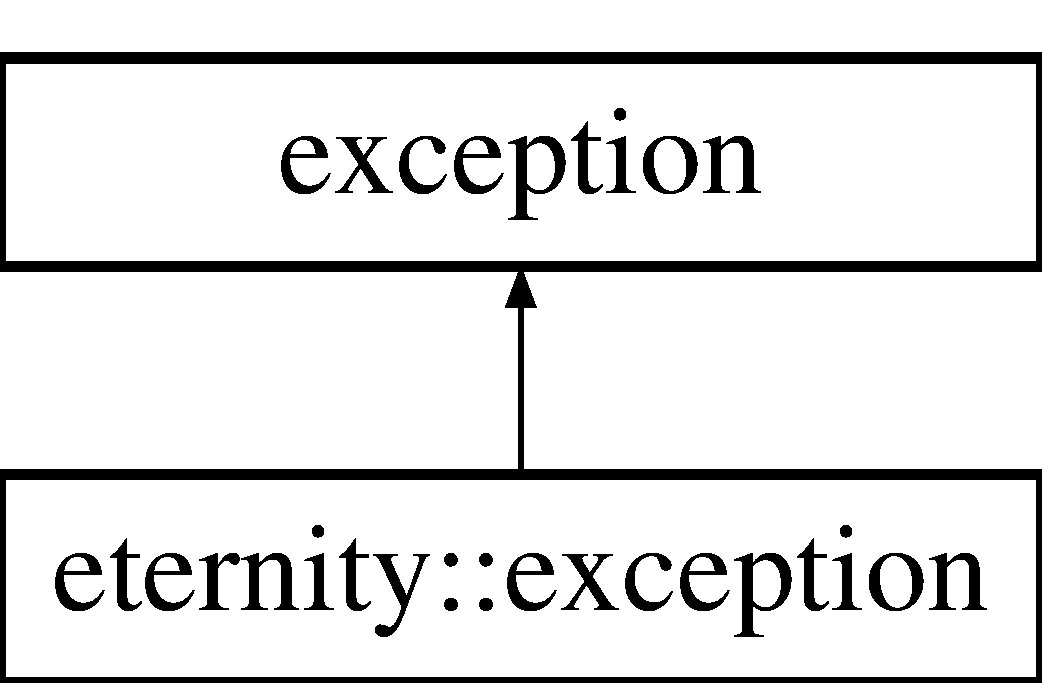
\includegraphics[height=2.000000cm]{classeternity_1_1exception}
\end{center}
\end{figure}
\subsection*{Public Member Functions}
\begin{DoxyCompactItemize}
\item 
\hyperlink{classeternity_1_1exception_a681b708eb4c5870221307180d685ea0f}{exception} (std\+::string swhat)
\item 
\hyperlink{classeternity_1_1exception_a68454ae0f538c10f63380c6d9954acab}{exception} (const \hyperlink{classeternity_1_1exception}{exception} \&right)
\item 
\hyperlink{classeternity_1_1exception}{exception} \& \hyperlink{classeternity_1_1exception_a9723617b72c37884f532451c578a3d39}{operator=} (const \hyperlink{classeternity_1_1exception}{exception} \&right)
\item 
virtual \hyperlink{classeternity_1_1exception_a88196166c38b9b66d790cf94be058e18}{$\sim$exception} ()  throw ()
\item 
virtual const char $\ast$ \hyperlink{classeternity_1_1exception_a5267219aab7b3bd423a6a751939928a6}{what} () const  throw ()
\end{DoxyCompactItemize}
\subsection*{Protected Attributes}
\begin{DoxyCompactItemize}
\item 
std\+::string \hyperlink{classeternity_1_1exception_ad3190da518fc2bb1dcc50fa665176036}{m\+\_\+swhat}
\end{DoxyCompactItemize}


\subsection{Detailed Description}


Definition at line 173 of file dynamic.\+hpp.



\subsection{Constructor \& Destructor Documentation}
\mbox{\Hypertarget{classeternity_1_1exception_a681b708eb4c5870221307180d685ea0f}\label{classeternity_1_1exception_a681b708eb4c5870221307180d685ea0f}} 
\index{eternity\+::exception@{eternity\+::exception}!exception@{exception}}
\index{exception@{exception}!eternity\+::exception@{eternity\+::exception}}
\subsubsection{\texorpdfstring{exception()}{exception()}\hspace{0.1cm}{\footnotesize\ttfamily [1/2]}}
{\footnotesize\ttfamily eternity\+::exception\+::exception (\begin{DoxyParamCaption}\item[{std\+::string}]{swhat }\end{DoxyParamCaption})}



Definition at line 41 of file dynamic.\+cpp.

\mbox{\Hypertarget{classeternity_1_1exception_a68454ae0f538c10f63380c6d9954acab}\label{classeternity_1_1exception_a68454ae0f538c10f63380c6d9954acab}} 
\index{eternity\+::exception@{eternity\+::exception}!exception@{exception}}
\index{exception@{exception}!eternity\+::exception@{eternity\+::exception}}
\subsubsection{\texorpdfstring{exception()}{exception()}\hspace{0.1cm}{\footnotesize\ttfamily [2/2]}}
{\footnotesize\ttfamily eternity\+::exception\+::exception (\begin{DoxyParamCaption}\item[{const \hyperlink{classeternity_1_1exception}{exception} \&}]{right }\end{DoxyParamCaption})\hspace{0.3cm}{\ttfamily [inline]}}



Definition at line 180 of file dynamic.\+hpp.

\mbox{\Hypertarget{classeternity_1_1exception_a88196166c38b9b66d790cf94be058e18}\label{classeternity_1_1exception_a88196166c38b9b66d790cf94be058e18}} 
\index{eternity\+::exception@{eternity\+::exception}!````~exception@{$\sim$exception}}
\index{````~exception@{$\sim$exception}!eternity\+::exception@{eternity\+::exception}}
\subsubsection{\texorpdfstring{$\sim$exception()}{~exception()}}
{\footnotesize\ttfamily eternity\+::exception\+::$\sim$exception (\begin{DoxyParamCaption}{ }\end{DoxyParamCaption}) throw  ) \hspace{0.3cm}{\ttfamily [virtual]}}



Definition at line 44 of file dynamic.\+cpp.



\subsection{Member Function Documentation}
\mbox{\Hypertarget{classeternity_1_1exception_a9723617b72c37884f532451c578a3d39}\label{classeternity_1_1exception_a9723617b72c37884f532451c578a3d39}} 
\index{eternity\+::exception@{eternity\+::exception}!operator=@{operator=}}
\index{operator=@{operator=}!eternity\+::exception@{eternity\+::exception}}
\subsubsection{\texorpdfstring{operator=()}{operator=()}}
{\footnotesize\ttfamily \hyperlink{classeternity_1_1exception}{exception}\& eternity\+::exception\+::operator= (\begin{DoxyParamCaption}\item[{const \hyperlink{classeternity_1_1exception}{exception} \&}]{right }\end{DoxyParamCaption})\hspace{0.3cm}{\ttfamily [inline]}}



Definition at line 184 of file dynamic.\+hpp.

\mbox{\Hypertarget{classeternity_1_1exception_a5267219aab7b3bd423a6a751939928a6}\label{classeternity_1_1exception_a5267219aab7b3bd423a6a751939928a6}} 
\index{eternity\+::exception@{eternity\+::exception}!what@{what}}
\index{what@{what}!eternity\+::exception@{eternity\+::exception}}
\subsubsection{\texorpdfstring{what()}{what()}}
{\footnotesize\ttfamily const char $\ast$ eternity\+::exception\+::what (\begin{DoxyParamCaption}{ }\end{DoxyParamCaption}) const throw  ) \hspace{0.3cm}{\ttfamily [virtual]}}



Definition at line 47 of file dynamic.\+cpp.



\subsection{Member Data Documentation}
\mbox{\Hypertarget{classeternity_1_1exception_ad3190da518fc2bb1dcc50fa665176036}\label{classeternity_1_1exception_ad3190da518fc2bb1dcc50fa665176036}} 
\index{eternity\+::exception@{eternity\+::exception}!m\+\_\+swhat@{m\+\_\+swhat}}
\index{m\+\_\+swhat@{m\+\_\+swhat}!eternity\+::exception@{eternity\+::exception}}
\subsubsection{\texorpdfstring{m\+\_\+swhat}{m\_swhat}}
{\footnotesize\ttfamily std\+::string eternity\+::exception\+::m\+\_\+swhat\hspace{0.3cm}{\ttfamily [protected]}}



Definition at line 175 of file dynamic.\+hpp.



The documentation for this class was generated from the following files\+:\begin{DoxyCompactItemize}
\item 
/home/filip/\+Ph\+D/\+W\+D\+F\+Pipe\+\_\+test/p4\+T\+S\+A/include/eternity/\hyperlink{dynamic_8hpp}{dynamic.\+hpp}\item 
/home/filip/\+Ph\+D/\+W\+D\+F\+Pipe\+\_\+test/p4\+T\+S\+A/include/eternity/\hyperlink{dynamic_8cpp}{dynamic.\+cpp}\end{DoxyCompactItemize}

\hypertarget{classeternity_1_1factory}{}\section{eternity\+:\+:factory$<$ t $>$ Class Template Reference}
\label{classeternity_1_1factory}\index{eternity\+::factory$<$ t $>$@{eternity\+::factory$<$ t $>$}}


{\ttfamily \#include $<$dynamic.\+hpp$>$}

Inheritance diagram for eternity\+:\+:factory$<$ t $>$\+:\begin{figure}[H]
\begin{center}
\leavevmode
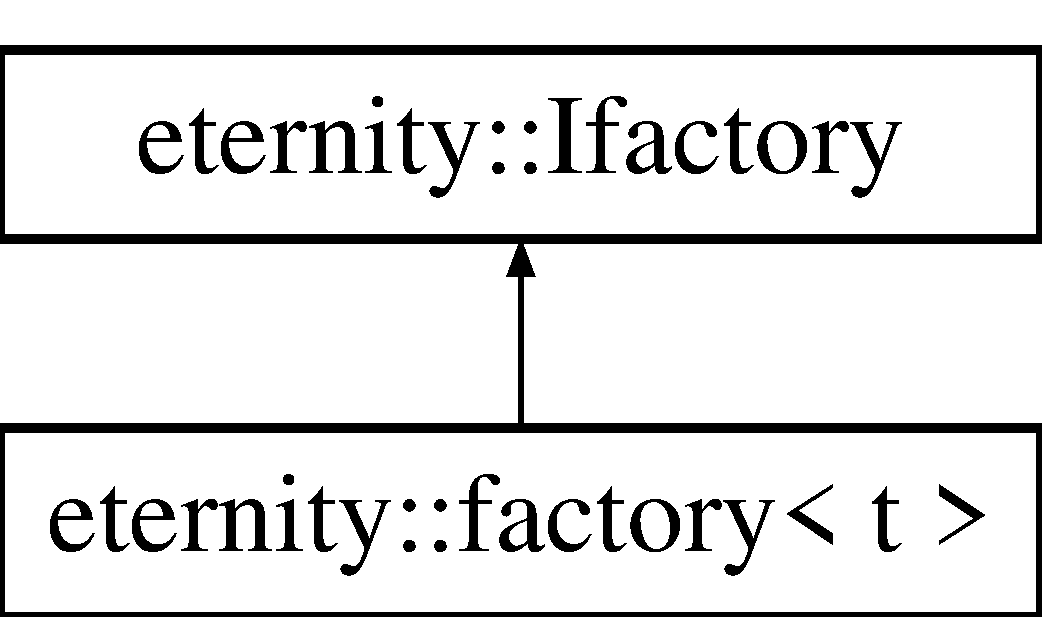
\includegraphics[height=2.000000cm]{classeternity_1_1factory}
\end{center}
\end{figure}
\subsection*{Public Member Functions}
\begin{DoxyCompactItemize}
\item 
\hyperlink{classeternity_1_1factory_a0fc6f0a6ec7ef7057f06924b948d8c94}{factory} ()
\begin{DoxyCompactList}\small\item\em Default constructor. \end{DoxyCompactList}\item 
\hyperlink{classeternity_1_1factory_aabaf1fee796b93628f897af8ac9c3ea9}{factory} (std\+::string conventional\+\_\+name)
\begin{DoxyCompactList}\small\item\em Constructor for cross compiler compatibility. \end{DoxyCompactList}\item 
virtual \hyperlink{classeternity_1_1factory_a5abc378892135b2d5491d7380752bb84}{$\sim$factory} ()
\begin{DoxyCompactList}\small\item\em Remove this from the gloab list of factory$<$t$>$ object. \end{DoxyCompactList}\item 
virtual void $\ast$ \hyperlink{classeternity_1_1factory_a08c1c494bc749955f9b0767d31933c2b}{create} (std\+::string \&class\+\_\+name)
\begin{DoxyCompactList}\small\item\em create an instance from class t if the same specified in class\+\_\+name \end{DoxyCompactList}\item 
virtual std\+::string \hyperlink{classeternity_1_1factory_a0b7c7bc194b178379eb1b880f87d3b48}{get\+\_\+conventional\+\_\+name} (std\+::string \&compiler\+\_\+name)
\end{DoxyCompactItemize}
\subsection*{Private Attributes}
\begin{DoxyCompactItemize}
\item 
std\+::string \hyperlink{classeternity_1_1factory_abf647d721a959e2a9728ff79b2bf094d}{m\+\_\+s\+Conventional\+Name}
\begin{DoxyCompactList}\small\item\em An istance of the object to dynamic create. \end{DoxyCompactList}\end{DoxyCompactItemize}
\subsection*{Additional Inherited Members}


\subsection{Detailed Description}
\subsubsection*{template$<$class t$>$\newline
class eternity\+::factory$<$ t $>$}

factory$<$t$>$ is responsable for the creation of object derived by the class t at run-\/time. 

Definition at line 70 of file dynamic.\+hpp.



\subsection{Constructor \& Destructor Documentation}
\mbox{\Hypertarget{classeternity_1_1factory_a0fc6f0a6ec7ef7057f06924b948d8c94}\label{classeternity_1_1factory_a0fc6f0a6ec7ef7057f06924b948d8c94}} 
\index{eternity\+::factory@{eternity\+::factory}!factory@{factory}}
\index{factory@{factory}!eternity\+::factory@{eternity\+::factory}}
\subsubsection{\texorpdfstring{factory()}{factory()}\hspace{0.1cm}{\footnotesize\ttfamily [1/2]}}
{\footnotesize\ttfamily template$<$class t $>$ \\
\hyperlink{classeternity_1_1factory}{eternity\+::factory}$<$ t $>$\+::\hyperlink{classeternity_1_1factory}{factory} (\begin{DoxyParamCaption}{ }\end{DoxyParamCaption})}



Default constructor. 

The default constructor that add this to the gloab list of factory$<$t$>$ object. 

Definition at line 106 of file dynamic.\+hpp.

\mbox{\Hypertarget{classeternity_1_1factory_aabaf1fee796b93628f897af8ac9c3ea9}\label{classeternity_1_1factory_aabaf1fee796b93628f897af8ac9c3ea9}} 
\index{eternity\+::factory@{eternity\+::factory}!factory@{factory}}
\index{factory@{factory}!eternity\+::factory@{eternity\+::factory}}
\subsubsection{\texorpdfstring{factory()}{factory()}\hspace{0.1cm}{\footnotesize\ttfamily [2/2]}}
{\footnotesize\ttfamily template$<$class t $>$ \\
\hyperlink{classeternity_1_1factory}{eternity\+::factory}$<$ t $>$\+::\hyperlink{classeternity_1_1factory}{factory} (\begin{DoxyParamCaption}\item[{std\+::string}]{conventional\+\_\+name }\end{DoxyParamCaption})}



Constructor for cross compiler compatibility. 



Definition at line 116 of file dynamic.\+hpp.

\mbox{\Hypertarget{classeternity_1_1factory_a5abc378892135b2d5491d7380752bb84}\label{classeternity_1_1factory_a5abc378892135b2d5491d7380752bb84}} 
\index{eternity\+::factory@{eternity\+::factory}!````~factory@{$\sim$factory}}
\index{````~factory@{$\sim$factory}!eternity\+::factory@{eternity\+::factory}}
\subsubsection{\texorpdfstring{$\sim$factory()}{~factory()}}
{\footnotesize\ttfamily template$<$class t $>$ \\
\hyperlink{classeternity_1_1factory}{eternity\+::factory}$<$ t $>$\+::$\sim$\hyperlink{classeternity_1_1factory}{factory} (\begin{DoxyParamCaption}{ }\end{DoxyParamCaption})\hspace{0.3cm}{\ttfamily [virtual]}}



Remove this from the gloab list of factory$<$t$>$ object. 



Definition at line 137 of file dynamic.\+hpp.



\subsection{Member Function Documentation}
\mbox{\Hypertarget{classeternity_1_1factory_a08c1c494bc749955f9b0767d31933c2b}\label{classeternity_1_1factory_a08c1c494bc749955f9b0767d31933c2b}} 
\index{eternity\+::factory@{eternity\+::factory}!create@{create}}
\index{create@{create}!eternity\+::factory@{eternity\+::factory}}
\subsubsection{\texorpdfstring{create()}{create()}}
{\footnotesize\ttfamily template$<$class t $>$ \\
void $\ast$ \hyperlink{classeternity_1_1factory}{eternity\+::factory}$<$ t $>$\+::create (\begin{DoxyParamCaption}\item[{std\+::string \&}]{class\+\_\+name }\end{DoxyParamCaption})\hspace{0.3cm}{\ttfamily [virtual]}}



create an instance from class t if the same specified in class\+\_\+name 

Return a pointer to a new istance of the class t (the only template parmeter of factory$<$t$>$) only if the string class\+\_\+name is actually the name of class t. Otherwise return a N\+U\+LL pointer 

Implements \hyperlink{classeternity_1_1_ifactory_afaca5a9abf52fa3a731c3dfed7cb73b3}{eternity\+::\+Ifactory}.



Definition at line 123 of file dynamic.\+hpp.

\mbox{\Hypertarget{classeternity_1_1factory_a0b7c7bc194b178379eb1b880f87d3b48}\label{classeternity_1_1factory_a0b7c7bc194b178379eb1b880f87d3b48}} 
\index{eternity\+::factory@{eternity\+::factory}!get\+\_\+conventional\+\_\+name@{get\+\_\+conventional\+\_\+name}}
\index{get\+\_\+conventional\+\_\+name@{get\+\_\+conventional\+\_\+name}!eternity\+::factory@{eternity\+::factory}}
\subsubsection{\texorpdfstring{get\+\_\+conventional\+\_\+name()}{get\_conventional\_name()}}
{\footnotesize\ttfamily template$<$class t $>$ \\
std\+::string \hyperlink{classeternity_1_1factory}{eternity\+::factory}$<$ t $>$\+::get\+\_\+conventional\+\_\+name (\begin{DoxyParamCaption}\item[{std\+::string \&}]{compiler\+\_\+name }\end{DoxyParamCaption})\hspace{0.3cm}{\ttfamily [virtual]}}

Return the conventional name of class t if typeid(t).name() match with compiler\+\_\+name. Otherwise return an empty. 

Implements \hyperlink{classeternity_1_1_ifactory_a6c2afa73d61aaa81233ab1216c508252}{eternity\+::\+Ifactory}.



Definition at line 130 of file dynamic.\+hpp.



\subsection{Member Data Documentation}
\mbox{\Hypertarget{classeternity_1_1factory_abf647d721a959e2a9728ff79b2bf094d}\label{classeternity_1_1factory_abf647d721a959e2a9728ff79b2bf094d}} 
\index{eternity\+::factory@{eternity\+::factory}!m\+\_\+s\+Conventional\+Name@{m\+\_\+s\+Conventional\+Name}}
\index{m\+\_\+s\+Conventional\+Name@{m\+\_\+s\+Conventional\+Name}!eternity\+::factory@{eternity\+::factory}}
\subsubsection{\texorpdfstring{m\+\_\+s\+Conventional\+Name}{m\_sConventionalName}}
{\footnotesize\ttfamily template$<$class t $>$ \\
std\+::string \hyperlink{classeternity_1_1factory}{eternity\+::factory}$<$ t $>$\+::m\+\_\+s\+Conventional\+Name\hspace{0.3cm}{\ttfamily [private]}}



An istance of the object to dynamic create. 



Definition at line 72 of file dynamic.\+hpp.



The documentation for this class was generated from the following file\+:\begin{DoxyCompactItemize}
\item 
/home/filip/\+Ph\+D/\+W\+D\+F\+Pipe\+\_\+test/p4\+T\+S\+A/include/eternity/\hyperlink{dynamic_8hpp}{dynamic.\+hpp}\end{DoxyCompactItemize}

\hypertarget{classtsa_1_1_fifo_buffer}{}\section{tsa\+:\+:Fifo\+Buffer Class Reference}
\label{classtsa_1_1_fifo_buffer}\index{tsa\+::\+Fifo\+Buffer@{tsa\+::\+Fifo\+Buffer}}


Band limited interpolation.  




{\ttfamily \#include $<$Fifo\+Buffer.\+hpp$>$}

\subsection*{Public Member Functions}
\begin{DoxyCompactItemize}
\item 
\hyperlink{classtsa_1_1_fifo_buffer_ad30fe947e5c2b34614859cbf12d749f1}{Fifo\+Buffer} (unsigned int channels)
\item 
\hyperlink{classtsa_1_1_fifo_buffer_ac6a76ca0fd208c80de6e4e04d5c43173}{Fifo\+Buffer} (const \hyperlink{classtsa_1_1_fifo_buffer}{Fifo\+Buffer} \&from)
\item 
\hyperlink{classtsa_1_1_fifo_buffer_ad7bec7c4fc528a12763f29c8f6a8e460}{$\sim$\+Fifo\+Buffer} ()
\item 
\hyperlink{classtsa_1_1_fifo_buffer}{Fifo\+Buffer} \& \hyperlink{classtsa_1_1_fifo_buffer_ad3c89a0f4aa3e475e136ec8c47f2165e}{operator=} (const \hyperlink{classtsa_1_1_fifo_buffer}{Fifo\+Buffer} \&from)
\end{DoxyCompactItemize}
\begin{Indent}\textbf{ Operations}\par
\begin{DoxyCompactItemize}
\item 
void \hyperlink{classtsa_1_1_fifo_buffer_ab70c4b3ba1a5356ab5384cd7f8638b0d}{Add\+Points} (\hyperlink{namespacetsa_ad260cd21c1891c4ed391fe788569aba4}{Dmatrix} \&data, double scale, int n=0, int offset=0)
\item 
void \hyperlink{classtsa_1_1_fifo_buffer_a7058127e3d126d9d6f434d3bf386c59b}{Add\+Point} (\hyperlink{namespacetsa_a8900fb03d849baf447a1a0efe2561fb2}{Dvector} \&data, double scale)
\item 
void \hyperlink{classtsa_1_1_fifo_buffer_a5cec8568b62047b4fb5b19c3fb44d28b}{Add\+Point} ()
\item 
double \& \hyperlink{classtsa_1_1_fifo_buffer_a4a799676b78f5bc80d48db4fe7d64853}{Back} (unsigned int i)
\item 
void \hyperlink{classtsa_1_1_fifo_buffer_a17acb27e83ab4af3667974660b58cb4e}{Del\+Points} (int n)
\item 
unsigned int \hyperlink{classtsa_1_1_fifo_buffer_a7c14d2ae86c581d1ccc427dccb3f1213}{Size} ()
\item 
double \& \hyperlink{classtsa_1_1_fifo_buffer_a78f313804a23e61fa57329b6a1f3df02}{operator()} (int r, int c)
\item 
void \hyperlink{classtsa_1_1_fifo_buffer_a597548e1842c157dfe1ade0f9e5cd121}{Load} (const char $\ast$filename, const char $\ast$fmt=\char`\"{}txt\char`\"{})
\item 
void \hyperlink{classtsa_1_1_fifo_buffer_aeb760c1c71644dc850395b838e47bcfb}{Save} (const char $\ast$filename, const char $\ast$fmt=\char`\"{}txt\char`\"{})
\item 
void \hyperlink{classtsa_1_1_fifo_buffer_a8ad8bf7c3935bf645b6cda8be7de441a}{xml\+\_\+serialize} (\hyperlink{classeternity_1_1xml__archive}{eternity\+::xml\+\_\+archive} \&xml, const char $\ast$prefix)
\end{DoxyCompactItemize}
\end{Indent}
\subsection*{Private Attributes}
\begin{DoxyCompactItemize}
\item 
unsigned int \hyperlink{classtsa_1_1_fifo_buffer_add6db36d6910a8b1efba4b2439f4b9c5}{m\+Channels}
\item 
std\+::queue$<$ \hyperlink{namespacetsa_a8900fb03d849baf447a1a0efe2561fb2}{Dvector} $\ast$ $>$ \hyperlink{classtsa_1_1_fifo_buffer_a538034e48a1c598fbbde1fefb9e92f91}{m\+Repository}
\item 
std\+::deque$<$ \hyperlink{namespacetsa_a8900fb03d849baf447a1a0efe2561fb2}{Dvector} $\ast$ $>$ \hyperlink{classtsa_1_1_fifo_buffer_aa8039b60b66e4e6bedd661352fff095f}{m\+Buffer}
\end{DoxyCompactItemize}


\subsection{Detailed Description}
Band limited interpolation. 

Definition at line 76 of file Fifo\+Buffer.\+hpp.



\subsection{Constructor \& Destructor Documentation}
\mbox{\Hypertarget{classtsa_1_1_fifo_buffer_ad30fe947e5c2b34614859cbf12d749f1}\label{classtsa_1_1_fifo_buffer_ad30fe947e5c2b34614859cbf12d749f1}} 
\index{tsa\+::\+Fifo\+Buffer@{tsa\+::\+Fifo\+Buffer}!Fifo\+Buffer@{Fifo\+Buffer}}
\index{Fifo\+Buffer@{Fifo\+Buffer}!tsa\+::\+Fifo\+Buffer@{tsa\+::\+Fifo\+Buffer}}
\subsubsection{\texorpdfstring{Fifo\+Buffer()}{FifoBuffer()}\hspace{0.1cm}{\footnotesize\ttfamily [1/2]}}
{\footnotesize\ttfamily tsa\+::\+Fifo\+Buffer\+::\+Fifo\+Buffer (\begin{DoxyParamCaption}\item[{unsigned int}]{channels }\end{DoxyParamCaption})}

Constructor.


\begin{DoxyParams}{Parameters}
{\em channels} & number of channels \\
\hline
\end{DoxyParams}


Definition at line 5 of file Fifo\+Buffer.\+cpp.

\mbox{\Hypertarget{classtsa_1_1_fifo_buffer_ac6a76ca0fd208c80de6e4e04d5c43173}\label{classtsa_1_1_fifo_buffer_ac6a76ca0fd208c80de6e4e04d5c43173}} 
\index{tsa\+::\+Fifo\+Buffer@{tsa\+::\+Fifo\+Buffer}!Fifo\+Buffer@{Fifo\+Buffer}}
\index{Fifo\+Buffer@{Fifo\+Buffer}!tsa\+::\+Fifo\+Buffer@{tsa\+::\+Fifo\+Buffer}}
\subsubsection{\texorpdfstring{Fifo\+Buffer()}{FifoBuffer()}\hspace{0.1cm}{\footnotesize\ttfamily [2/2]}}
{\footnotesize\ttfamily tsa\+::\+Fifo\+Buffer\+::\+Fifo\+Buffer (\begin{DoxyParamCaption}\item[{const \hyperlink{classtsa_1_1_fifo_buffer}{Fifo\+Buffer} \&}]{from }\end{DoxyParamCaption})}

Copy constructor


\begin{DoxyParams}{Parameters}
{\em from} & The instance that must be copied \\
\hline
\end{DoxyParams}


Definition at line 12 of file Fifo\+Buffer.\+cpp.

\mbox{\Hypertarget{classtsa_1_1_fifo_buffer_ad7bec7c4fc528a12763f29c8f6a8e460}\label{classtsa_1_1_fifo_buffer_ad7bec7c4fc528a12763f29c8f6a8e460}} 
\index{tsa\+::\+Fifo\+Buffer@{tsa\+::\+Fifo\+Buffer}!````~Fifo\+Buffer@{$\sim$\+Fifo\+Buffer}}
\index{````~Fifo\+Buffer@{$\sim$\+Fifo\+Buffer}!tsa\+::\+Fifo\+Buffer@{tsa\+::\+Fifo\+Buffer}}
\subsubsection{\texorpdfstring{$\sim$\+Fifo\+Buffer()}{~FifoBuffer()}}
{\footnotesize\ttfamily tsa\+::\+Fifo\+Buffer\+::$\sim$\+Fifo\+Buffer (\begin{DoxyParamCaption}{ }\end{DoxyParamCaption})}

Destructor 

Definition at line 18 of file Fifo\+Buffer.\+cpp.



\subsection{Member Function Documentation}
\mbox{\Hypertarget{classtsa_1_1_fifo_buffer_a7058127e3d126d9d6f434d3bf386c59b}\label{classtsa_1_1_fifo_buffer_a7058127e3d126d9d6f434d3bf386c59b}} 
\index{tsa\+::\+Fifo\+Buffer@{tsa\+::\+Fifo\+Buffer}!Add\+Point@{Add\+Point}}
\index{Add\+Point@{Add\+Point}!tsa\+::\+Fifo\+Buffer@{tsa\+::\+Fifo\+Buffer}}
\subsubsection{\texorpdfstring{Add\+Point()}{AddPoint()}\hspace{0.1cm}{\footnotesize\ttfamily [1/2]}}
{\footnotesize\ttfamily void tsa\+::\+Fifo\+Buffer\+::\+Add\+Point (\begin{DoxyParamCaption}\item[{\hyperlink{namespacetsa_a8900fb03d849baf447a1a0efe2561fb2}{Dvector} \&}]{data,  }\item[{double}]{scale }\end{DoxyParamCaption})}

Insert in the back of the buffer a single data contained in a vector


\begin{DoxyParams}{Parameters}
{\em data} & the vector containing the data that must be inserted in the buffer \\
\hline
{\em scale} & the scale of the data \\
\hline
\end{DoxyParams}


Definition at line 57 of file Fifo\+Buffer.\+cpp.

\mbox{\Hypertarget{classtsa_1_1_fifo_buffer_a5cec8568b62047b4fb5b19c3fb44d28b}\label{classtsa_1_1_fifo_buffer_a5cec8568b62047b4fb5b19c3fb44d28b}} 
\index{tsa\+::\+Fifo\+Buffer@{tsa\+::\+Fifo\+Buffer}!Add\+Point@{Add\+Point}}
\index{Add\+Point@{Add\+Point}!tsa\+::\+Fifo\+Buffer@{tsa\+::\+Fifo\+Buffer}}
\subsubsection{\texorpdfstring{Add\+Point()}{AddPoint()}\hspace{0.1cm}{\footnotesize\ttfamily [2/2]}}
{\footnotesize\ttfamily void tsa\+::\+Fifo\+Buffer\+::\+Add\+Point (\begin{DoxyParamCaption}{ }\end{DoxyParamCaption})}

Insert in the back of the buffer a single uninitialized data 

Definition at line 48 of file Fifo\+Buffer.\+cpp.

\mbox{\Hypertarget{classtsa_1_1_fifo_buffer_ab70c4b3ba1a5356ab5384cd7f8638b0d}\label{classtsa_1_1_fifo_buffer_ab70c4b3ba1a5356ab5384cd7f8638b0d}} 
\index{tsa\+::\+Fifo\+Buffer@{tsa\+::\+Fifo\+Buffer}!Add\+Points@{Add\+Points}}
\index{Add\+Points@{Add\+Points}!tsa\+::\+Fifo\+Buffer@{tsa\+::\+Fifo\+Buffer}}
\subsubsection{\texorpdfstring{Add\+Points()}{AddPoints()}}
{\footnotesize\ttfamily void tsa\+::\+Fifo\+Buffer\+::\+Add\+Points (\begin{DoxyParamCaption}\item[{\hyperlink{namespacetsa_ad260cd21c1891c4ed391fe788569aba4}{Dmatrix} \&}]{data,  }\item[{double}]{scale,  }\item[{int}]{n = {\ttfamily 0},  }\item[{int}]{offset = {\ttfamily 0} }\end{DoxyParamCaption})}

Insert in the back of the buffer n data contained in a matrix, starting from a given offset. If n = 0 (default) all the data starting from the offset are copied.


\begin{DoxyParams}{Parameters}
{\em data} & the matrix containing the data that must be inserted in the buffer \\
\hline
{\em n} & the number of data to insert \\
\hline
{\em offset} & the offset of the data to insert \\
\hline
\end{DoxyParams}


Definition at line 72 of file Fifo\+Buffer.\+cpp.

\mbox{\Hypertarget{classtsa_1_1_fifo_buffer_a4a799676b78f5bc80d48db4fe7d64853}\label{classtsa_1_1_fifo_buffer_a4a799676b78f5bc80d48db4fe7d64853}} 
\index{tsa\+::\+Fifo\+Buffer@{tsa\+::\+Fifo\+Buffer}!Back@{Back}}
\index{Back@{Back}!tsa\+::\+Fifo\+Buffer@{tsa\+::\+Fifo\+Buffer}}
\subsubsection{\texorpdfstring{Back()}{Back()}}
{\footnotesize\ttfamily double\& tsa\+::\+Fifo\+Buffer\+::\+Back (\begin{DoxyParamCaption}\item[{unsigned int}]{i }\end{DoxyParamCaption})\hspace{0.3cm}{\ttfamily [inline]}}

Access to the last inserted data


\begin{DoxyParams}{Parameters}
{\em i} & the index inside the last inserted data\\
\hline
\end{DoxyParams}
\begin{DoxyReturn}{Returns}
reference to the last inserted data 
\end{DoxyReturn}


Definition at line 158 of file Fifo\+Buffer.\+hpp.

\mbox{\Hypertarget{classtsa_1_1_fifo_buffer_a17acb27e83ab4af3667974660b58cb4e}\label{classtsa_1_1_fifo_buffer_a17acb27e83ab4af3667974660b58cb4e}} 
\index{tsa\+::\+Fifo\+Buffer@{tsa\+::\+Fifo\+Buffer}!Del\+Points@{Del\+Points}}
\index{Del\+Points@{Del\+Points}!tsa\+::\+Fifo\+Buffer@{tsa\+::\+Fifo\+Buffer}}
\subsubsection{\texorpdfstring{Del\+Points()}{DelPoints()}}
{\footnotesize\ttfamily void tsa\+::\+Fifo\+Buffer\+::\+Del\+Points (\begin{DoxyParamCaption}\item[{int}]{n }\end{DoxyParamCaption})}

Delete some data from the front of the buffer.


\begin{DoxyParams}{Parameters}
{\em n} & number of data to delete \\
\hline
\end{DoxyParams}


Definition at line 93 of file Fifo\+Buffer.\+cpp.

\mbox{\Hypertarget{classtsa_1_1_fifo_buffer_a597548e1842c157dfe1ade0f9e5cd121}\label{classtsa_1_1_fifo_buffer_a597548e1842c157dfe1ade0f9e5cd121}} 
\index{tsa\+::\+Fifo\+Buffer@{tsa\+::\+Fifo\+Buffer}!Load@{Load}}
\index{Load@{Load}!tsa\+::\+Fifo\+Buffer@{tsa\+::\+Fifo\+Buffer}}
\subsubsection{\texorpdfstring{Load()}{Load()}}
{\footnotesize\ttfamily void tsa\+::\+Fifo\+Buffer\+::\+Load (\begin{DoxyParamCaption}\item[{const char $\ast$}]{filename,  }\item[{const char $\ast$}]{fmt = {\ttfamily \char`\"{}txt\char`\"{}} }\end{DoxyParamCaption})\hspace{0.3cm}{\ttfamily [inline]}}



Definition at line 192 of file Fifo\+Buffer.\+hpp.

\mbox{\Hypertarget{classtsa_1_1_fifo_buffer_a78f313804a23e61fa57329b6a1f3df02}\label{classtsa_1_1_fifo_buffer_a78f313804a23e61fa57329b6a1f3df02}} 
\index{tsa\+::\+Fifo\+Buffer@{tsa\+::\+Fifo\+Buffer}!operator()@{operator()}}
\index{operator()@{operator()}!tsa\+::\+Fifo\+Buffer@{tsa\+::\+Fifo\+Buffer}}
\subsubsection{\texorpdfstring{operator()()}{operator()()}}
{\footnotesize\ttfamily double\& tsa\+::\+Fifo\+Buffer\+::operator() (\begin{DoxyParamCaption}\item[{int}]{r,  }\item[{int}]{c }\end{DoxyParamCaption})\hspace{0.3cm}{\ttfamily [inline]}}

Access to the buffer data.


\begin{DoxyParams}{Parameters}
{\em r} & buffer row \\
\hline
{\em c} & buffer column\\
\hline
\end{DoxyParams}
\begin{DoxyReturn}{Returns}
the data 
\end{DoxyReturn}


Definition at line 188 of file Fifo\+Buffer.\+hpp.

\mbox{\Hypertarget{classtsa_1_1_fifo_buffer_ad3c89a0f4aa3e475e136ec8c47f2165e}\label{classtsa_1_1_fifo_buffer_ad3c89a0f4aa3e475e136ec8c47f2165e}} 
\index{tsa\+::\+Fifo\+Buffer@{tsa\+::\+Fifo\+Buffer}!operator=@{operator=}}
\index{operator=@{operator=}!tsa\+::\+Fifo\+Buffer@{tsa\+::\+Fifo\+Buffer}}
\subsubsection{\texorpdfstring{operator=()}{operator=()}}
{\footnotesize\ttfamily \hyperlink{classtsa_1_1_fifo_buffer}{Fifo\+Buffer} \& tsa\+::\+Fifo\+Buffer\+::operator= (\begin{DoxyParamCaption}\item[{const \hyperlink{classtsa_1_1_fifo_buffer}{Fifo\+Buffer} \&}]{from }\end{DoxyParamCaption})}

Assignement operator


\begin{DoxyParams}{Parameters}
{\em from} & The instance to be assigned from\\
\hline
\end{DoxyParams}
\begin{DoxyReturn}{Returns}
a reference to a new object 
\end{DoxyReturn}


Definition at line 31 of file Fifo\+Buffer.\+cpp.

\mbox{\Hypertarget{classtsa_1_1_fifo_buffer_aeb760c1c71644dc850395b838e47bcfb}\label{classtsa_1_1_fifo_buffer_aeb760c1c71644dc850395b838e47bcfb}} 
\index{tsa\+::\+Fifo\+Buffer@{tsa\+::\+Fifo\+Buffer}!Save@{Save}}
\index{Save@{Save}!tsa\+::\+Fifo\+Buffer@{tsa\+::\+Fifo\+Buffer}}
\subsubsection{\texorpdfstring{Save()}{Save()}}
{\footnotesize\ttfamily void tsa\+::\+Fifo\+Buffer\+::\+Save (\begin{DoxyParamCaption}\item[{const char $\ast$}]{filename,  }\item[{const char $\ast$}]{fmt = {\ttfamily \char`\"{}txt\char`\"{}} }\end{DoxyParamCaption})\hspace{0.3cm}{\ttfamily [inline]}}



Definition at line 199 of file Fifo\+Buffer.\+hpp.

\mbox{\Hypertarget{classtsa_1_1_fifo_buffer_a7c14d2ae86c581d1ccc427dccb3f1213}\label{classtsa_1_1_fifo_buffer_a7c14d2ae86c581d1ccc427dccb3f1213}} 
\index{tsa\+::\+Fifo\+Buffer@{tsa\+::\+Fifo\+Buffer}!Size@{Size}}
\index{Size@{Size}!tsa\+::\+Fifo\+Buffer@{tsa\+::\+Fifo\+Buffer}}
\subsubsection{\texorpdfstring{Size()}{Size()}}
{\footnotesize\ttfamily unsigned int tsa\+::\+Fifo\+Buffer\+::\+Size (\begin{DoxyParamCaption}{ }\end{DoxyParamCaption})\hspace{0.3cm}{\ttfamily [inline]}}

Get the present size of the buffer.

\begin{DoxyReturn}{Returns}
the size of the buffer 
\end{DoxyReturn}


Definition at line 176 of file Fifo\+Buffer.\+hpp.

\mbox{\Hypertarget{classtsa_1_1_fifo_buffer_a8ad8bf7c3935bf645b6cda8be7de441a}\label{classtsa_1_1_fifo_buffer_a8ad8bf7c3935bf645b6cda8be7de441a}} 
\index{tsa\+::\+Fifo\+Buffer@{tsa\+::\+Fifo\+Buffer}!xml\+\_\+serialize@{xml\+\_\+serialize}}
\index{xml\+\_\+serialize@{xml\+\_\+serialize}!tsa\+::\+Fifo\+Buffer@{tsa\+::\+Fifo\+Buffer}}
\subsubsection{\texorpdfstring{xml\+\_\+serialize()}{xml\_serialize()}}
{\footnotesize\ttfamily void tsa\+::\+Fifo\+Buffer\+::xml\+\_\+serialize (\begin{DoxyParamCaption}\item[{\hyperlink{classeternity_1_1xml__archive}{eternity\+::xml\+\_\+archive} \&}]{xml,  }\item[{const char $\ast$}]{prefix }\end{DoxyParamCaption})\hspace{0.3cm}{\ttfamily [inline]}}



Definition at line 206 of file Fifo\+Buffer.\+hpp.



\subsection{Member Data Documentation}
\mbox{\Hypertarget{classtsa_1_1_fifo_buffer_aa8039b60b66e4e6bedd661352fff095f}\label{classtsa_1_1_fifo_buffer_aa8039b60b66e4e6bedd661352fff095f}} 
\index{tsa\+::\+Fifo\+Buffer@{tsa\+::\+Fifo\+Buffer}!m\+Buffer@{m\+Buffer}}
\index{m\+Buffer@{m\+Buffer}!tsa\+::\+Fifo\+Buffer@{tsa\+::\+Fifo\+Buffer}}
\subsubsection{\texorpdfstring{m\+Buffer}{mBuffer}}
{\footnotesize\ttfamily std\+::deque$<$\hyperlink{namespacetsa_a8900fb03d849baf447a1a0efe2561fb2}{Dvector}$\ast$$>$ tsa\+::\+Fifo\+Buffer\+::m\+Buffer\hspace{0.3cm}{\ttfamily [private]}}

Buffer for incoming data points 

Definition at line 268 of file Fifo\+Buffer.\+hpp.

\mbox{\Hypertarget{classtsa_1_1_fifo_buffer_add6db36d6910a8b1efba4b2439f4b9c5}\label{classtsa_1_1_fifo_buffer_add6db36d6910a8b1efba4b2439f4b9c5}} 
\index{tsa\+::\+Fifo\+Buffer@{tsa\+::\+Fifo\+Buffer}!m\+Channels@{m\+Channels}}
\index{m\+Channels@{m\+Channels}!tsa\+::\+Fifo\+Buffer@{tsa\+::\+Fifo\+Buffer}}
\subsubsection{\texorpdfstring{m\+Channels}{mChannels}}
{\footnotesize\ttfamily unsigned int tsa\+::\+Fifo\+Buffer\+::m\+Channels\hspace{0.3cm}{\ttfamily [private]}}

Number of channels to resample 

Definition at line 266 of file Fifo\+Buffer.\+hpp.

\mbox{\Hypertarget{classtsa_1_1_fifo_buffer_a538034e48a1c598fbbde1fefb9e92f91}\label{classtsa_1_1_fifo_buffer_a538034e48a1c598fbbde1fefb9e92f91}} 
\index{tsa\+::\+Fifo\+Buffer@{tsa\+::\+Fifo\+Buffer}!m\+Repository@{m\+Repository}}
\index{m\+Repository@{m\+Repository}!tsa\+::\+Fifo\+Buffer@{tsa\+::\+Fifo\+Buffer}}
\subsubsection{\texorpdfstring{m\+Repository}{mRepository}}
{\footnotesize\ttfamily std\+::queue$<$\hyperlink{namespacetsa_a8900fb03d849baf447a1a0efe2561fb2}{Dvector}$\ast$$>$ tsa\+::\+Fifo\+Buffer\+::m\+Repository\hspace{0.3cm}{\ttfamily [private]}}

Repository for unused data points 

Definition at line 267 of file Fifo\+Buffer.\+hpp.



The documentation for this class was generated from the following files\+:\begin{DoxyCompactItemize}
\item 
/home/filip/\+Ph\+D/\+W\+D\+F\+Pipe\+\_\+test/p4\+T\+S\+A/include/\hyperlink{_fifo_buffer_8hpp}{Fifo\+Buffer.\+hpp}\item 
/home/filip/\+Ph\+D/\+W\+D\+F\+Pipe\+\_\+test/p4\+T\+S\+A/src/\hyperlink{_fifo_buffer_8cpp}{Fifo\+Buffer.\+cpp}\end{DoxyCompactItemize}

\hypertarget{classeternity_1_1file__archive}{}\section{eternity\+:\+:file\+\_\+archive Class Reference}
\label{classeternity_1_1file__archive}\index{eternity\+::file\+\_\+archive@{eternity\+::file\+\_\+archive}}


{\ttfamily \#include $<$persist.\+hpp$>$}

Inheritance diagram for eternity\+:\+:file\+\_\+archive\+:\begin{figure}[H]
\begin{center}
\leavevmode
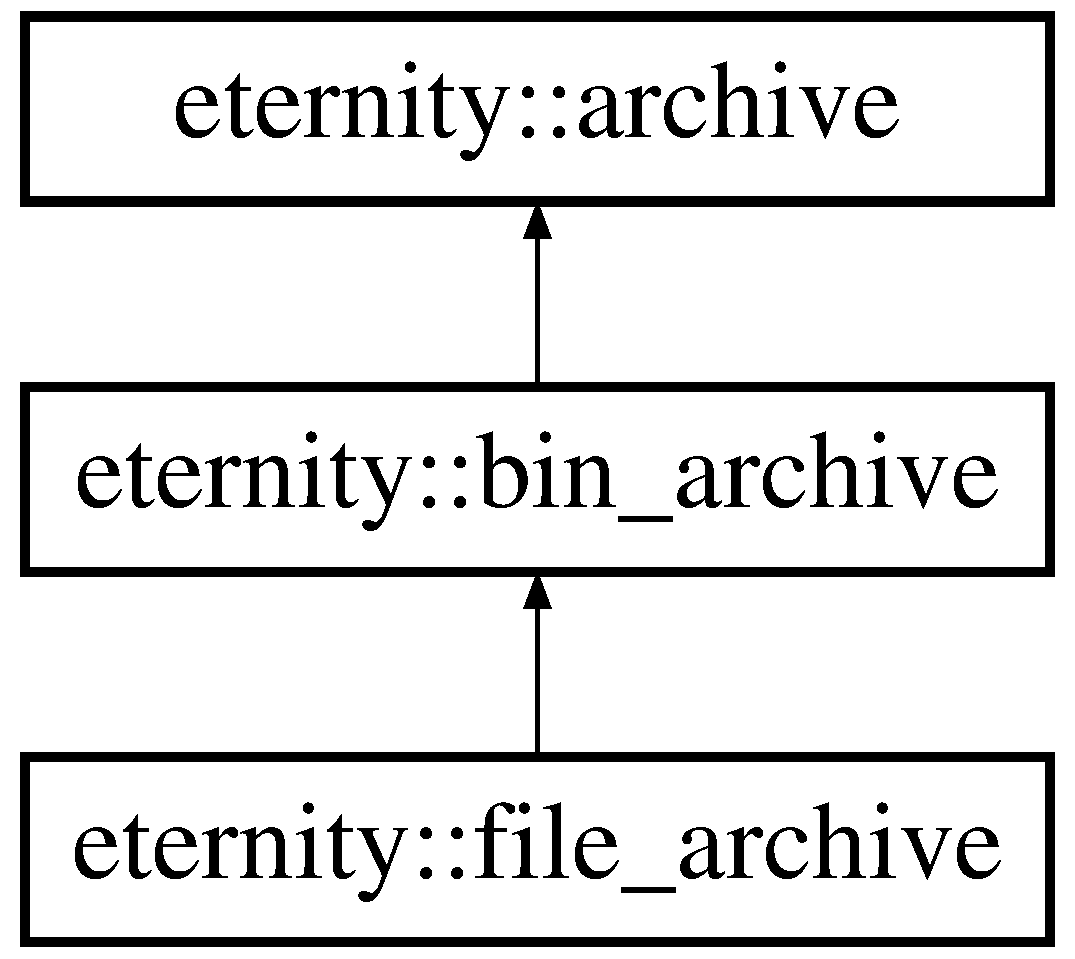
\includegraphics[height=3.000000cm]{classeternity_1_1file__archive}
\end{center}
\end{figure}
\subsection*{Public Member Functions}
\begin{DoxyCompactItemize}
\item 
\hyperlink{classeternity_1_1file__archive_ab2a892aad41300e922115115b76b7754}{file\+\_\+archive} ()
\item 
\hyperlink{classeternity_1_1file__archive_a6f7dd96ce65d0be588f31286313a4b5a}{file\+\_\+archive} (std\+::string file\+\_\+name, \hyperlink{classeternity_1_1archive_a8881f9ce8dbed2ee600c64b7925afef0}{opening\+\_\+mode} mode)
\item 
\hyperlink{classeternity_1_1file__archive_a122b37e9949cd1a2f6279ed23d01d97f}{$\sim$file\+\_\+archive} ()
\item 
void \hyperlink{classeternity_1_1file__archive_aa42b3bfaf4e595f61ec07bec48676d46}{close} ()
\begin{DoxyCompactList}\small\item\em close the archive file and release memory used. \end{DoxyCompactList}\item 
void \hyperlink{classeternity_1_1file__archive_a64a17edf2cea4f1582a5a3c44eb86fa4}{open} (std\+::string file\+\_\+name, \hyperlink{classeternity_1_1archive_a8881f9ce8dbed2ee600c64b7925afef0}{opening\+\_\+mode} mode)
\item 
void \hyperlink{classeternity_1_1file__archive_a5f97e0b816c5d9406f675b25f34c21f8}{open} (std\+::string s\+Name, bool loading=true)
\begin{DoxyCompactList}\small\item\em open the archive file and update this for the serialization \end{DoxyCompactList}\item 
virtual size\+\_\+t \hyperlink{classeternity_1_1file__archive_a0eaf4b5937b3ff46df3627f64efc19e8}{write} (const void $\ast$buffer, size\+\_\+t size, size\+\_\+t count)
\begin{DoxyCompactList}\small\item\em write a buffer of a certain legnth n time in the archive \end{DoxyCompactList}\item 
virtual size\+\_\+t \hyperlink{classeternity_1_1file__archive_a307b43ac9f06c7077ac0f7e48dc0d7ab}{read} (void $\ast$buffer, size\+\_\+t size, size\+\_\+t count)
\begin{DoxyCompactList}\small\item\em read a buffer of a certain legnth n time in the archive \end{DoxyCompactList}\end{DoxyCompactItemize}
\subsection*{Private Attributes}
\begin{DoxyCompactItemize}
\item 
std\+::fstream \hyperlink{classeternity_1_1file__archive_ac702d57d9633f8695476da8a7d55dd9d}{stream}
\end{DoxyCompactItemize}
\subsection*{Additional Inherited Members}


\subsection{Detailed Description}
Realize an binary archive using the common file like stream. 

Definition at line 193 of file persist.\+hpp.



\subsection{Constructor \& Destructor Documentation}
\mbox{\Hypertarget{classeternity_1_1file__archive_ab2a892aad41300e922115115b76b7754}\label{classeternity_1_1file__archive_ab2a892aad41300e922115115b76b7754}} 
\index{eternity\+::file\+\_\+archive@{eternity\+::file\+\_\+archive}!file\+\_\+archive@{file\+\_\+archive}}
\index{file\+\_\+archive@{file\+\_\+archive}!eternity\+::file\+\_\+archive@{eternity\+::file\+\_\+archive}}
\subsubsection{\texorpdfstring{file\+\_\+archive()}{file\_archive()}\hspace{0.1cm}{\footnotesize\ttfamily [1/2]}}
{\footnotesize\ttfamily eternity\+::file\+\_\+archive\+::file\+\_\+archive (\begin{DoxyParamCaption}{ }\end{DoxyParamCaption})\hspace{0.3cm}{\ttfamily [inline]}}



Definition at line 197 of file persist.\+hpp.

\mbox{\Hypertarget{classeternity_1_1file__archive_a6f7dd96ce65d0be588f31286313a4b5a}\label{classeternity_1_1file__archive_a6f7dd96ce65d0be588f31286313a4b5a}} 
\index{eternity\+::file\+\_\+archive@{eternity\+::file\+\_\+archive}!file\+\_\+archive@{file\+\_\+archive}}
\index{file\+\_\+archive@{file\+\_\+archive}!eternity\+::file\+\_\+archive@{eternity\+::file\+\_\+archive}}
\subsubsection{\texorpdfstring{file\+\_\+archive()}{file\_archive()}\hspace{0.1cm}{\footnotesize\ttfamily [2/2]}}
{\footnotesize\ttfamily eternity\+::file\+\_\+archive\+::file\+\_\+archive (\begin{DoxyParamCaption}\item[{std\+::string}]{file\+\_\+name,  }\item[{\hyperlink{classeternity_1_1archive_a8881f9ce8dbed2ee600c64b7925afef0}{opening\+\_\+mode}}]{mode }\end{DoxyParamCaption})}



Definition at line 73 of file persist.\+cpp.

\mbox{\Hypertarget{classeternity_1_1file__archive_a122b37e9949cd1a2f6279ed23d01d97f}\label{classeternity_1_1file__archive_a122b37e9949cd1a2f6279ed23d01d97f}} 
\index{eternity\+::file\+\_\+archive@{eternity\+::file\+\_\+archive}!````~file\+\_\+archive@{$\sim$file\+\_\+archive}}
\index{````~file\+\_\+archive@{$\sim$file\+\_\+archive}!eternity\+::file\+\_\+archive@{eternity\+::file\+\_\+archive}}
\subsubsection{\texorpdfstring{$\sim$file\+\_\+archive()}{~file\_archive()}}
{\footnotesize\ttfamily eternity\+::file\+\_\+archive\+::$\sim$file\+\_\+archive (\begin{DoxyParamCaption}{ }\end{DoxyParamCaption})\hspace{0.3cm}{\ttfamily [inline]}}



Definition at line 203 of file persist.\+hpp.



\subsection{Member Function Documentation}
\mbox{\Hypertarget{classeternity_1_1file__archive_aa42b3bfaf4e595f61ec07bec48676d46}\label{classeternity_1_1file__archive_aa42b3bfaf4e595f61ec07bec48676d46}} 
\index{eternity\+::file\+\_\+archive@{eternity\+::file\+\_\+archive}!close@{close}}
\index{close@{close}!eternity\+::file\+\_\+archive@{eternity\+::file\+\_\+archive}}
\subsubsection{\texorpdfstring{close()}{close()}}
{\footnotesize\ttfamily void eternity\+::file\+\_\+archive\+::close (\begin{DoxyParamCaption}{ }\end{DoxyParamCaption})\hspace{0.3cm}{\ttfamily [inline]}}



close the archive file and release memory used. 



Definition at line 209 of file persist.\+hpp.

\mbox{\Hypertarget{classeternity_1_1file__archive_a64a17edf2cea4f1582a5a3c44eb86fa4}\label{classeternity_1_1file__archive_a64a17edf2cea4f1582a5a3c44eb86fa4}} 
\index{eternity\+::file\+\_\+archive@{eternity\+::file\+\_\+archive}!open@{open}}
\index{open@{open}!eternity\+::file\+\_\+archive@{eternity\+::file\+\_\+archive}}
\subsubsection{\texorpdfstring{open()}{open()}\hspace{0.1cm}{\footnotesize\ttfamily [1/2]}}
{\footnotesize\ttfamily void eternity\+::file\+\_\+archive\+::open (\begin{DoxyParamCaption}\item[{std\+::string}]{file\+\_\+name,  }\item[{\hyperlink{classeternity_1_1archive_a8881f9ce8dbed2ee600c64b7925afef0}{opening\+\_\+mode}}]{mode }\end{DoxyParamCaption})}

initialize the \hyperlink{classeternity_1_1file__archive}{file\+\_\+archive} using the file named file\+\_\+name. If mode is load create the file. Anyway init update archive to begin persistence operations. 

Definition at line 99 of file persist.\+cpp.

\mbox{\Hypertarget{classeternity_1_1file__archive_a5f97e0b816c5d9406f675b25f34c21f8}\label{classeternity_1_1file__archive_a5f97e0b816c5d9406f675b25f34c21f8}} 
\index{eternity\+::file\+\_\+archive@{eternity\+::file\+\_\+archive}!open@{open}}
\index{open@{open}!eternity\+::file\+\_\+archive@{eternity\+::file\+\_\+archive}}
\subsubsection{\texorpdfstring{open()}{open()}\hspace{0.1cm}{\footnotesize\ttfamily [2/2]}}
{\footnotesize\ttfamily void eternity\+::file\+\_\+archive\+::open (\begin{DoxyParamCaption}\item[{std\+::string}]{s\+Name,  }\item[{bool}]{loading = {\ttfamily true} }\end{DoxyParamCaption})}



open the archive file and update this for the serialization 



Definition at line 105 of file persist.\+cpp.

\mbox{\Hypertarget{classeternity_1_1file__archive_a307b43ac9f06c7077ac0f7e48dc0d7ab}\label{classeternity_1_1file__archive_a307b43ac9f06c7077ac0f7e48dc0d7ab}} 
\index{eternity\+::file\+\_\+archive@{eternity\+::file\+\_\+archive}!read@{read}}
\index{read@{read}!eternity\+::file\+\_\+archive@{eternity\+::file\+\_\+archive}}
\subsubsection{\texorpdfstring{read()}{read()}}
{\footnotesize\ttfamily size\+\_\+t eternity\+::file\+\_\+archive\+::read (\begin{DoxyParamCaption}\item[{void $\ast$}]{buffer,  }\item[{size\+\_\+t}]{size,  }\item[{size\+\_\+t}]{count }\end{DoxyParamCaption})\hspace{0.3cm}{\ttfamily [virtual]}}



read a buffer of a certain legnth n time in the archive 



Implements \hyperlink{classeternity_1_1bin__archive_a5d67b032541f5a1e104d2fcd0eaa7a55}{eternity\+::bin\+\_\+archive}.



Definition at line 86 of file persist.\+cpp.

\mbox{\Hypertarget{classeternity_1_1file__archive_a0eaf4b5937b3ff46df3627f64efc19e8}\label{classeternity_1_1file__archive_a0eaf4b5937b3ff46df3627f64efc19e8}} 
\index{eternity\+::file\+\_\+archive@{eternity\+::file\+\_\+archive}!write@{write}}
\index{write@{write}!eternity\+::file\+\_\+archive@{eternity\+::file\+\_\+archive}}
\subsubsection{\texorpdfstring{write()}{write()}}
{\footnotesize\ttfamily size\+\_\+t eternity\+::file\+\_\+archive\+::write (\begin{DoxyParamCaption}\item[{const void $\ast$}]{buffer,  }\item[{size\+\_\+t}]{size,  }\item[{size\+\_\+t}]{count }\end{DoxyParamCaption})\hspace{0.3cm}{\ttfamily [virtual]}}



write a buffer of a certain legnth n time in the archive 



Implements \hyperlink{classeternity_1_1bin__archive_acbe041b0815f2721ee18ad042557b14e}{eternity\+::bin\+\_\+archive}.



Definition at line 77 of file persist.\+cpp.



\subsection{Member Data Documentation}
\mbox{\Hypertarget{classeternity_1_1file__archive_ac702d57d9633f8695476da8a7d55dd9d}\label{classeternity_1_1file__archive_ac702d57d9633f8695476da8a7d55dd9d}} 
\index{eternity\+::file\+\_\+archive@{eternity\+::file\+\_\+archive}!stream@{stream}}
\index{stream@{stream}!eternity\+::file\+\_\+archive@{eternity\+::file\+\_\+archive}}
\subsubsection{\texorpdfstring{stream}{stream}}
{\footnotesize\ttfamily std\+::fstream eternity\+::file\+\_\+archive\+::stream\hspace{0.3cm}{\ttfamily [private]}}



Definition at line 194 of file persist.\+hpp.



The documentation for this class was generated from the following files\+:\begin{DoxyCompactItemize}
\item 
/home/filip/\+Ph\+D/\+W\+D\+F\+Pipe\+\_\+test/p4\+T\+S\+A/include/eternity/\hyperlink{persist_8hpp}{persist.\+hpp}\item 
/home/filip/\+Ph\+D/\+W\+D\+F\+Pipe\+\_\+test/p4\+T\+S\+A/include/eternity/\hyperlink{persist_8cpp}{persist.\+cpp}\end{DoxyCompactItemize}

\hypertarget{classtsa_1_1_f_r_a_m_e_h___channel}{}\section{tsa\+:\+:F\+R\+A\+M\+E\+H\+\_\+\+Channel Class Reference}
\label{classtsa_1_1_f_r_a_m_e_h___channel}\index{tsa\+::\+F\+R\+A\+M\+E\+H\+\_\+\+Channel@{tsa\+::\+F\+R\+A\+M\+E\+H\+\_\+\+Channel}}


{\ttfamily \#include $<$Frame\+I\+Stream.\+hpp$>$}

Inheritance diagram for tsa\+:\+:F\+R\+A\+M\+E\+H\+\_\+\+Channel\+:\begin{figure}[H]
\begin{center}
\leavevmode
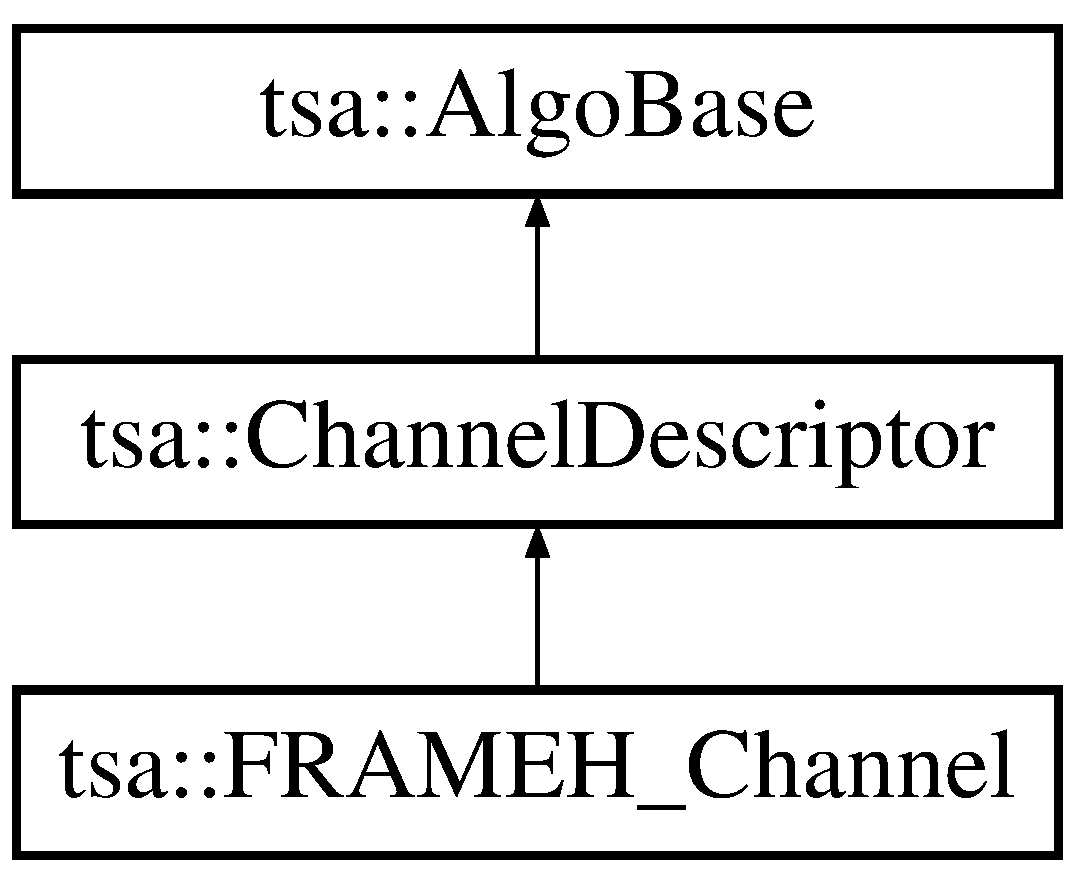
\includegraphics[height=3.000000cm]{classtsa_1_1_f_r_a_m_e_h___channel}
\end{center}
\end{figure}
\subsection*{Public Types}
\begin{DoxyCompactItemize}
\item 
enum \hyperlink{classtsa_1_1_f_r_a_m_e_h___channel_af9bd3bfda5ebc40f65e8af27abac9fe3}{field\+\_\+type} \{ \newline
\hyperlink{classtsa_1_1_f_r_a_m_e_h___channel_af9bd3bfda5ebc40f65e8af27abac9fe3a11936056dc8f51d020db82b4cd4cd5b3}{field\+\_\+run}, 
\hyperlink{classtsa_1_1_f_r_a_m_e_h___channel_af9bd3bfda5ebc40f65e8af27abac9fe3a37f297e43f3378c404b42391c9ece6bf}{field\+\_\+frame}, 
\hyperlink{classtsa_1_1_f_r_a_m_e_h___channel_af9bd3bfda5ebc40f65e8af27abac9fe3ae1cd9acd47598e9f3473148b6fcc09d4}{field\+\_\+data\+Quality}, 
\hyperlink{classtsa_1_1_f_r_a_m_e_h___channel_af9bd3bfda5ebc40f65e8af27abac9fe3a93b921e1acc87fa78badf6e4bc4552d7}{field\+\_\+\+G\+TimeS}, 
\newline
\hyperlink{classtsa_1_1_f_r_a_m_e_h___channel_af9bd3bfda5ebc40f65e8af27abac9fe3ab14b559f3bf02d8c2dfbcd71b0a2f17b}{field\+\_\+\+G\+TimeN}, 
\hyperlink{classtsa_1_1_f_r_a_m_e_h___channel_af9bd3bfda5ebc40f65e8af27abac9fe3add897c0e122b716817814e73f0afef3b}{field\+\_\+\+U\+LeapS}, 
\hyperlink{classtsa_1_1_f_r_a_m_e_h___channel_af9bd3bfda5ebc40f65e8af27abac9fe3aa467146fdc3b2c4bd49bf0f301d3fad5}{field\+\_\+dt}, 
\hyperlink{classtsa_1_1_f_r_a_m_e_h___channel_af9bd3bfda5ebc40f65e8af27abac9fe3a7aa7e4e96809decee1afe9a7583b0ae8}{field\+\_\+time}
 \}
\end{DoxyCompactItemize}
\subsection*{Public Member Functions}
\begin{DoxyCompactItemize}
\item 
\hyperlink{classtsa_1_1_f_r_a_m_e_h___channel_a27a8bc2d9aba282cb68f855c49b2eaba}{F\+R\+A\+M\+E\+H\+\_\+\+Channel} (\hyperlink{classtsa_1_1_frame_i_stream}{Frame\+I\+Stream} $\ast$F\+IS, enum \hyperlink{classtsa_1_1_f_r_a_m_e_h___channel_af9bd3bfda5ebc40f65e8af27abac9fe3}{field\+\_\+type} ft, unsigned int id)
\item 
virtual \hyperlink{classtsa_1_1_f_r_a_m_e_h___channel_a6174aa904d4e084e77695f8e19b8fcd2}{$\sim$\+F\+R\+A\+M\+E\+H\+\_\+\+Channel} ()
\item 
virtual void \hyperlink{classtsa_1_1_f_r_a_m_e_h___channel_af757e23c465da95ac0ed7b97876ead66}{Add\+Data} ()
\item 
virtual double \hyperlink{classtsa_1_1_f_r_a_m_e_h___channel_a022b134fb62d99e8cb00a6ce28b2d569}{Get\+Length} ()
\end{DoxyCompactItemize}
\subsection*{Static Public Member Functions}
\begin{DoxyCompactItemize}
\item 
static \hyperlink{classtsa_1_1_f_r_a_m_e_h___channel}{F\+R\+A\+M\+E\+H\+\_\+\+Channel} $\ast$ \hyperlink{classtsa_1_1_f_r_a_m_e_h___channel_a9a920292ece110df4cdce41f9f8e451b}{Create} (\hyperlink{classtsa_1_1_frame_i_stream}{Frame\+I\+Stream} $\ast$F\+IS, char $\ast$field\+\_\+name, unsigned int id)
\end{DoxyCompactItemize}
\subsection*{Private Attributes}
\begin{DoxyCompactItemize}
\item 
char $\ast$ \hyperlink{classtsa_1_1_f_r_a_m_e_h___channel_aff87ea1426812c4e02ccaa741774db29}{m\+Field\+Name}
\item 
enum \hyperlink{classtsa_1_1_f_r_a_m_e_h___channel_af9bd3bfda5ebc40f65e8af27abac9fe3}{field\+\_\+type} \hyperlink{classtsa_1_1_f_r_a_m_e_h___channel_a3a63c899c18c606c39c2cd32859d3b05}{m\+Field\+Type}
\end{DoxyCompactItemize}
\subsection*{Additional Inherited Members}


\subsection{Detailed Description}
Descriptor for a FrameH field channel. 

Definition at line 456 of file Frame\+I\+Stream.\+hpp.



\subsection{Member Enumeration Documentation}
\mbox{\Hypertarget{classtsa_1_1_f_r_a_m_e_h___channel_af9bd3bfda5ebc40f65e8af27abac9fe3}\label{classtsa_1_1_f_r_a_m_e_h___channel_af9bd3bfda5ebc40f65e8af27abac9fe3}} 
\index{tsa\+::\+F\+R\+A\+M\+E\+H\+\_\+\+Channel@{tsa\+::\+F\+R\+A\+M\+E\+H\+\_\+\+Channel}!field\+\_\+type@{field\+\_\+type}}
\index{field\+\_\+type@{field\+\_\+type}!tsa\+::\+F\+R\+A\+M\+E\+H\+\_\+\+Channel@{tsa\+::\+F\+R\+A\+M\+E\+H\+\_\+\+Channel}}
\subsubsection{\texorpdfstring{field\+\_\+type}{field\_type}}
{\footnotesize\ttfamily enum \hyperlink{classtsa_1_1_f_r_a_m_e_h___channel_af9bd3bfda5ebc40f65e8af27abac9fe3}{tsa\+::\+F\+R\+A\+M\+E\+H\+\_\+\+Channel\+::field\+\_\+type}}

Field type in the frame to dump on channel \begin{DoxyEnumFields}{Enumerator}
\raisebox{\heightof{T}}[0pt][0pt]{\index{field\+\_\+run@{field\+\_\+run}!tsa\+::\+F\+R\+A\+M\+E\+H\+\_\+\+Channel@{tsa\+::\+F\+R\+A\+M\+E\+H\+\_\+\+Channel}}\index{tsa\+::\+F\+R\+A\+M\+E\+H\+\_\+\+Channel@{tsa\+::\+F\+R\+A\+M\+E\+H\+\_\+\+Channel}!field\+\_\+run@{field\+\_\+run}}}\mbox{\Hypertarget{classtsa_1_1_f_r_a_m_e_h___channel_af9bd3bfda5ebc40f65e8af27abac9fe3a11936056dc8f51d020db82b4cd4cd5b3}\label{classtsa_1_1_f_r_a_m_e_h___channel_af9bd3bfda5ebc40f65e8af27abac9fe3a11936056dc8f51d020db82b4cd4cd5b3}} 
field\+\_\+run&Run number \\
\hline

\raisebox{\heightof{T}}[0pt][0pt]{\index{field\+\_\+frame@{field\+\_\+frame}!tsa\+::\+F\+R\+A\+M\+E\+H\+\_\+\+Channel@{tsa\+::\+F\+R\+A\+M\+E\+H\+\_\+\+Channel}}\index{tsa\+::\+F\+R\+A\+M\+E\+H\+\_\+\+Channel@{tsa\+::\+F\+R\+A\+M\+E\+H\+\_\+\+Channel}!field\+\_\+frame@{field\+\_\+frame}}}\mbox{\Hypertarget{classtsa_1_1_f_r_a_m_e_h___channel_af9bd3bfda5ebc40f65e8af27abac9fe3a37f297e43f3378c404b42391c9ece6bf}\label{classtsa_1_1_f_r_a_m_e_h___channel_af9bd3bfda5ebc40f65e8af27abac9fe3a37f297e43f3378c404b42391c9ece6bf}} 
field\+\_\+frame&Frame number \\
\hline

\raisebox{\heightof{T}}[0pt][0pt]{\index{field\+\_\+data\+Quality@{field\+\_\+data\+Quality}!tsa\+::\+F\+R\+A\+M\+E\+H\+\_\+\+Channel@{tsa\+::\+F\+R\+A\+M\+E\+H\+\_\+\+Channel}}\index{tsa\+::\+F\+R\+A\+M\+E\+H\+\_\+\+Channel@{tsa\+::\+F\+R\+A\+M\+E\+H\+\_\+\+Channel}!field\+\_\+data\+Quality@{field\+\_\+data\+Quality}}}\mbox{\Hypertarget{classtsa_1_1_f_r_a_m_e_h___channel_af9bd3bfda5ebc40f65e8af27abac9fe3ae1cd9acd47598e9f3473148b6fcc09d4}\label{classtsa_1_1_f_r_a_m_e_h___channel_af9bd3bfda5ebc40f65e8af27abac9fe3ae1cd9acd47598e9f3473148b6fcc09d4}} 
field\+\_\+data\+Quality&Data quality \\
\hline

\raisebox{\heightof{T}}[0pt][0pt]{\index{field\+\_\+\+G\+TimeS@{field\+\_\+\+G\+TimeS}!tsa\+::\+F\+R\+A\+M\+E\+H\+\_\+\+Channel@{tsa\+::\+F\+R\+A\+M\+E\+H\+\_\+\+Channel}}\index{tsa\+::\+F\+R\+A\+M\+E\+H\+\_\+\+Channel@{tsa\+::\+F\+R\+A\+M\+E\+H\+\_\+\+Channel}!field\+\_\+\+G\+TimeS@{field\+\_\+\+G\+TimeS}}}\mbox{\Hypertarget{classtsa_1_1_f_r_a_m_e_h___channel_af9bd3bfda5ebc40f65e8af27abac9fe3a93b921e1acc87fa78badf6e4bc4552d7}\label{classtsa_1_1_f_r_a_m_e_h___channel_af9bd3bfda5ebc40f65e8af27abac9fe3a93b921e1acc87fa78badf6e4bc4552d7}} 
field\+\_\+\+G\+TimeS&G\+TimeS \\
\hline

\raisebox{\heightof{T}}[0pt][0pt]{\index{field\+\_\+\+G\+TimeN@{field\+\_\+\+G\+TimeN}!tsa\+::\+F\+R\+A\+M\+E\+H\+\_\+\+Channel@{tsa\+::\+F\+R\+A\+M\+E\+H\+\_\+\+Channel}}\index{tsa\+::\+F\+R\+A\+M\+E\+H\+\_\+\+Channel@{tsa\+::\+F\+R\+A\+M\+E\+H\+\_\+\+Channel}!field\+\_\+\+G\+TimeN@{field\+\_\+\+G\+TimeN}}}\mbox{\Hypertarget{classtsa_1_1_f_r_a_m_e_h___channel_af9bd3bfda5ebc40f65e8af27abac9fe3ab14b559f3bf02d8c2dfbcd71b0a2f17b}\label{classtsa_1_1_f_r_a_m_e_h___channel_af9bd3bfda5ebc40f65e8af27abac9fe3ab14b559f3bf02d8c2dfbcd71b0a2f17b}} 
field\+\_\+\+G\+TimeN&G\+TimeN \\
\hline

\raisebox{\heightof{T}}[0pt][0pt]{\index{field\+\_\+\+U\+LeapS@{field\+\_\+\+U\+LeapS}!tsa\+::\+F\+R\+A\+M\+E\+H\+\_\+\+Channel@{tsa\+::\+F\+R\+A\+M\+E\+H\+\_\+\+Channel}}\index{tsa\+::\+F\+R\+A\+M\+E\+H\+\_\+\+Channel@{tsa\+::\+F\+R\+A\+M\+E\+H\+\_\+\+Channel}!field\+\_\+\+U\+LeapS@{field\+\_\+\+U\+LeapS}}}\mbox{\Hypertarget{classtsa_1_1_f_r_a_m_e_h___channel_af9bd3bfda5ebc40f65e8af27abac9fe3add897c0e122b716817814e73f0afef3b}\label{classtsa_1_1_f_r_a_m_e_h___channel_af9bd3bfda5ebc40f65e8af27abac9fe3add897c0e122b716817814e73f0afef3b}} 
field\+\_\+\+U\+LeapS&U\+LeapS \\
\hline

\raisebox{\heightof{T}}[0pt][0pt]{\index{field\+\_\+dt@{field\+\_\+dt}!tsa\+::\+F\+R\+A\+M\+E\+H\+\_\+\+Channel@{tsa\+::\+F\+R\+A\+M\+E\+H\+\_\+\+Channel}}\index{tsa\+::\+F\+R\+A\+M\+E\+H\+\_\+\+Channel@{tsa\+::\+F\+R\+A\+M\+E\+H\+\_\+\+Channel}!field\+\_\+dt@{field\+\_\+dt}}}\mbox{\Hypertarget{classtsa_1_1_f_r_a_m_e_h___channel_af9bd3bfda5ebc40f65e8af27abac9fe3aa467146fdc3b2c4bd49bf0f301d3fad5}\label{classtsa_1_1_f_r_a_m_e_h___channel_af9bd3bfda5ebc40f65e8af27abac9fe3aa467146fdc3b2c4bd49bf0f301d3fad5}} 
field\+\_\+dt&dt \\
\hline

\raisebox{\heightof{T}}[0pt][0pt]{\index{field\+\_\+time@{field\+\_\+time}!tsa\+::\+F\+R\+A\+M\+E\+H\+\_\+\+Channel@{tsa\+::\+F\+R\+A\+M\+E\+H\+\_\+\+Channel}}\index{tsa\+::\+F\+R\+A\+M\+E\+H\+\_\+\+Channel@{tsa\+::\+F\+R\+A\+M\+E\+H\+\_\+\+Channel}!field\+\_\+time@{field\+\_\+time}}}\mbox{\Hypertarget{classtsa_1_1_f_r_a_m_e_h___channel_af9bd3bfda5ebc40f65e8af27abac9fe3a7aa7e4e96809decee1afe9a7583b0ae8}\label{classtsa_1_1_f_r_a_m_e_h___channel_af9bd3bfda5ebc40f65e8af27abac9fe3a7aa7e4e96809decee1afe9a7583b0ae8}} 
field\+\_\+time&time \\
\hline

\end{DoxyEnumFields}


Definition at line 463 of file Frame\+I\+Stream.\+hpp.



\subsection{Constructor \& Destructor Documentation}
\mbox{\Hypertarget{classtsa_1_1_f_r_a_m_e_h___channel_a27a8bc2d9aba282cb68f855c49b2eaba}\label{classtsa_1_1_f_r_a_m_e_h___channel_a27a8bc2d9aba282cb68f855c49b2eaba}} 
\index{tsa\+::\+F\+R\+A\+M\+E\+H\+\_\+\+Channel@{tsa\+::\+F\+R\+A\+M\+E\+H\+\_\+\+Channel}!F\+R\+A\+M\+E\+H\+\_\+\+Channel@{F\+R\+A\+M\+E\+H\+\_\+\+Channel}}
\index{F\+R\+A\+M\+E\+H\+\_\+\+Channel@{F\+R\+A\+M\+E\+H\+\_\+\+Channel}!tsa\+::\+F\+R\+A\+M\+E\+H\+\_\+\+Channel@{tsa\+::\+F\+R\+A\+M\+E\+H\+\_\+\+Channel}}
\subsubsection{\texorpdfstring{F\+R\+A\+M\+E\+H\+\_\+\+Channel()}{FRAMEH\_Channel()}}
{\footnotesize\ttfamily tsa\+::\+F\+R\+A\+M\+E\+H\+\_\+\+Channel\+::\+F\+R\+A\+M\+E\+H\+\_\+\+Channel (\begin{DoxyParamCaption}\item[{\hyperlink{classtsa_1_1_frame_i_stream}{Frame\+I\+Stream} $\ast$}]{F\+IS,  }\item[{enum \hyperlink{classtsa_1_1_f_r_a_m_e_h___channel_af9bd3bfda5ebc40f65e8af27abac9fe3}{field\+\_\+type}}]{ft,  }\item[{unsigned int}]{id }\end{DoxyParamCaption})}

Constructor


\begin{DoxyParams}{Parameters}
{\em F\+IS} & pointer to the \hyperlink{classtsa_1_1_frame_i_stream}{Frame\+I\+Stream} class \\
\hline
{\em ft} & the field type of the requested channel \\
\hline
{\em id} & id of the channel \\
\hline
\end{DoxyParams}


Definition at line 474 of file Frame\+I\+Stream.\+cpp.

\mbox{\Hypertarget{classtsa_1_1_f_r_a_m_e_h___channel_a6174aa904d4e084e77695f8e19b8fcd2}\label{classtsa_1_1_f_r_a_m_e_h___channel_a6174aa904d4e084e77695f8e19b8fcd2}} 
\index{tsa\+::\+F\+R\+A\+M\+E\+H\+\_\+\+Channel@{tsa\+::\+F\+R\+A\+M\+E\+H\+\_\+\+Channel}!````~F\+R\+A\+M\+E\+H\+\_\+\+Channel@{$\sim$\+F\+R\+A\+M\+E\+H\+\_\+\+Channel}}
\index{````~F\+R\+A\+M\+E\+H\+\_\+\+Channel@{$\sim$\+F\+R\+A\+M\+E\+H\+\_\+\+Channel}!tsa\+::\+F\+R\+A\+M\+E\+H\+\_\+\+Channel@{tsa\+::\+F\+R\+A\+M\+E\+H\+\_\+\+Channel}}
\subsubsection{\texorpdfstring{$\sim$\+F\+R\+A\+M\+E\+H\+\_\+\+Channel()}{~FRAMEH\_Channel()}}
{\footnotesize\ttfamily tsa\+::\+F\+R\+A\+M\+E\+H\+\_\+\+Channel\+::$\sim$\+F\+R\+A\+M\+E\+H\+\_\+\+Channel (\begin{DoxyParamCaption}{ }\end{DoxyParamCaption})\hspace{0.3cm}{\ttfamily [virtual]}}

Destructor 

Definition at line 527 of file Frame\+I\+Stream.\+cpp.



\subsection{Member Function Documentation}
\mbox{\Hypertarget{classtsa_1_1_f_r_a_m_e_h___channel_af757e23c465da95ac0ed7b97876ead66}\label{classtsa_1_1_f_r_a_m_e_h___channel_af757e23c465da95ac0ed7b97876ead66}} 
\index{tsa\+::\+F\+R\+A\+M\+E\+H\+\_\+\+Channel@{tsa\+::\+F\+R\+A\+M\+E\+H\+\_\+\+Channel}!Add\+Data@{Add\+Data}}
\index{Add\+Data@{Add\+Data}!tsa\+::\+F\+R\+A\+M\+E\+H\+\_\+\+Channel@{tsa\+::\+F\+R\+A\+M\+E\+H\+\_\+\+Channel}}
\subsubsection{\texorpdfstring{Add\+Data()}{AddData()}}
{\footnotesize\ttfamily void tsa\+::\+F\+R\+A\+M\+E\+H\+\_\+\+Channel\+::\+Add\+Data (\begin{DoxyParamCaption}{ }\end{DoxyParamCaption})\hspace{0.3cm}{\ttfamily [virtual]}}

This function must be called when there are not enough data to fill the output view. It reads a chunk of data from the current frame. 

Reimplemented from \hyperlink{classtsa_1_1_channel_descriptor_aa1e001a5e712415cd4e9d66846914a56}{tsa\+::\+Channel\+Descriptor}.



Definition at line 531 of file Frame\+I\+Stream.\+cpp.

\mbox{\Hypertarget{classtsa_1_1_f_r_a_m_e_h___channel_a9a920292ece110df4cdce41f9f8e451b}\label{classtsa_1_1_f_r_a_m_e_h___channel_a9a920292ece110df4cdce41f9f8e451b}} 
\index{tsa\+::\+F\+R\+A\+M\+E\+H\+\_\+\+Channel@{tsa\+::\+F\+R\+A\+M\+E\+H\+\_\+\+Channel}!Create@{Create}}
\index{Create@{Create}!tsa\+::\+F\+R\+A\+M\+E\+H\+\_\+\+Channel@{tsa\+::\+F\+R\+A\+M\+E\+H\+\_\+\+Channel}}
\subsubsection{\texorpdfstring{Create()}{Create()}}
{\footnotesize\ttfamily \hyperlink{classtsa_1_1_f_r_a_m_e_h___channel}{F\+R\+A\+M\+E\+H\+\_\+\+Channel} $\ast$ tsa\+::\+F\+R\+A\+M\+E\+H\+\_\+\+Channel\+::\+Create (\begin{DoxyParamCaption}\item[{\hyperlink{classtsa_1_1_frame_i_stream}{Frame\+I\+Stream} $\ast$}]{F\+IS,  }\item[{char $\ast$}]{field\+\_\+name,  }\item[{unsigned int}]{id }\end{DoxyParamCaption})\hspace{0.3cm}{\ttfamily [static]}}

Create, if possible, an instance of the class


\begin{DoxyParams}{Parameters}
{\em F\+IS} & pointer to the \hyperlink{classtsa_1_1_frame_i_stream}{Frame\+I\+Stream} class instance \\
\hline
{\em name} & name of the channel \\
\hline
{\em id} & index of the channel\\
\hline
\end{DoxyParams}
\begin{DoxyReturn}{Returns}
pointer to the created class instance or null 
\end{DoxyReturn}


Definition at line 418 of file Frame\+I\+Stream.\+cpp.

\mbox{\Hypertarget{classtsa_1_1_f_r_a_m_e_h___channel_a022b134fb62d99e8cb00a6ce28b2d569}\label{classtsa_1_1_f_r_a_m_e_h___channel_a022b134fb62d99e8cb00a6ce28b2d569}} 
\index{tsa\+::\+F\+R\+A\+M\+E\+H\+\_\+\+Channel@{tsa\+::\+F\+R\+A\+M\+E\+H\+\_\+\+Channel}!Get\+Length@{Get\+Length}}
\index{Get\+Length@{Get\+Length}!tsa\+::\+F\+R\+A\+M\+E\+H\+\_\+\+Channel@{tsa\+::\+F\+R\+A\+M\+E\+H\+\_\+\+Channel}}
\subsubsection{\texorpdfstring{Get\+Length()}{GetLength()}}
{\footnotesize\ttfamily double tsa\+::\+F\+R\+A\+M\+E\+H\+\_\+\+Channel\+::\+Get\+Length (\begin{DoxyParamCaption}{ }\end{DoxyParamCaption})\hspace{0.3cm}{\ttfamily [virtual]}}

Get the maximul time length of data that can be currently filled without calling Add\+Data.

\begin{DoxyReturn}{Returns}
the time length of the data available in seconds 
\end{DoxyReturn}


Reimplemented from \hyperlink{classtsa_1_1_channel_descriptor_a456d14e6136c389fbd307fabab7d7b73}{tsa\+::\+Channel\+Descriptor}.



Definition at line 567 of file Frame\+I\+Stream.\+cpp.



\subsection{Member Data Documentation}
\mbox{\Hypertarget{classtsa_1_1_f_r_a_m_e_h___channel_aff87ea1426812c4e02ccaa741774db29}\label{classtsa_1_1_f_r_a_m_e_h___channel_aff87ea1426812c4e02ccaa741774db29}} 
\index{tsa\+::\+F\+R\+A\+M\+E\+H\+\_\+\+Channel@{tsa\+::\+F\+R\+A\+M\+E\+H\+\_\+\+Channel}!m\+Field\+Name@{m\+Field\+Name}}
\index{m\+Field\+Name@{m\+Field\+Name}!tsa\+::\+F\+R\+A\+M\+E\+H\+\_\+\+Channel@{tsa\+::\+F\+R\+A\+M\+E\+H\+\_\+\+Channel}}
\subsubsection{\texorpdfstring{m\+Field\+Name}{mFieldName}}
{\footnotesize\ttfamily char$\ast$ tsa\+::\+F\+R\+A\+M\+E\+H\+\_\+\+Channel\+::m\+Field\+Name\hspace{0.3cm}{\ttfamily [private]}}

Field name 

Definition at line 518 of file Frame\+I\+Stream.\+hpp.

\mbox{\Hypertarget{classtsa_1_1_f_r_a_m_e_h___channel_a3a63c899c18c606c39c2cd32859d3b05}\label{classtsa_1_1_f_r_a_m_e_h___channel_a3a63c899c18c606c39c2cd32859d3b05}} 
\index{tsa\+::\+F\+R\+A\+M\+E\+H\+\_\+\+Channel@{tsa\+::\+F\+R\+A\+M\+E\+H\+\_\+\+Channel}!m\+Field\+Type@{m\+Field\+Type}}
\index{m\+Field\+Type@{m\+Field\+Type}!tsa\+::\+F\+R\+A\+M\+E\+H\+\_\+\+Channel@{tsa\+::\+F\+R\+A\+M\+E\+H\+\_\+\+Channel}}
\subsubsection{\texorpdfstring{m\+Field\+Type}{mFieldType}}
{\footnotesize\ttfamily enum \hyperlink{classtsa_1_1_f_r_a_m_e_h___channel_af9bd3bfda5ebc40f65e8af27abac9fe3}{field\+\_\+type} tsa\+::\+F\+R\+A\+M\+E\+H\+\_\+\+Channel\+::m\+Field\+Type\hspace{0.3cm}{\ttfamily [private]}}

Field type 

Definition at line 519 of file Frame\+I\+Stream.\+hpp.



The documentation for this class was generated from the following files\+:\begin{DoxyCompactItemize}
\item 
/home/filip/\+Ph\+D/\+W\+D\+F\+Pipe\+\_\+test/p4\+T\+S\+A/include/\hyperlink{_frame_i_stream_8hpp}{Frame\+I\+Stream.\+hpp}\item 
/home/filip/\+Ph\+D/\+W\+D\+F\+Pipe\+\_\+test/p4\+T\+S\+A/src/\hyperlink{_frame_i_stream_8cpp}{Frame\+I\+Stream.\+cpp}\end{DoxyCompactItemize}

\hypertarget{classtsa_1_1_frame_i_channel}{}\section{tsa\+:\+:Frame\+I\+Channel Class Reference}
\label{classtsa_1_1_frame_i_channel}\index{tsa\+::\+Frame\+I\+Channel@{tsa\+::\+Frame\+I\+Channel}}


A source of data taken from a Frame file.  




{\ttfamily \#include $<$Frame\+I\+Channel.\+hpp$>$}

Inheritance diagram for tsa\+:\+:Frame\+I\+Channel\+:\begin{figure}[H]
\begin{center}
\leavevmode
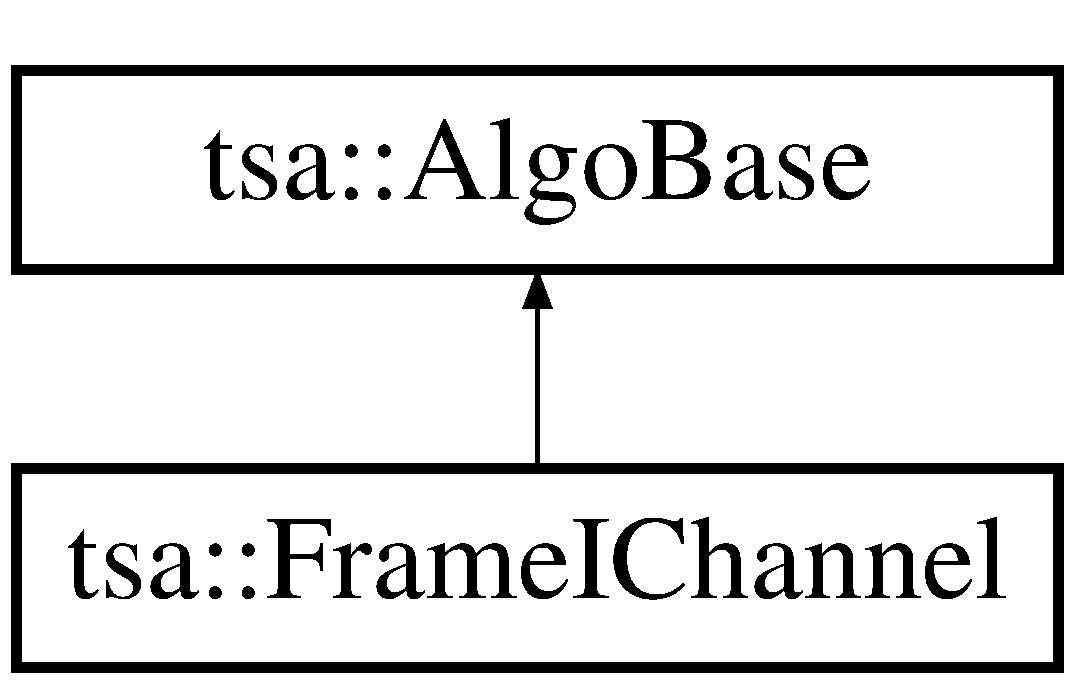
\includegraphics[height=2.000000cm]{classtsa_1_1_frame_i_channel}
\end{center}
\end{figure}
\subsection*{Public Member Functions}
\begin{DoxyCompactItemize}
\item 
\hyperlink{classtsa_1_1_frame_i_channel_acc55687d86116d3cc2db6c4d2b2e7c1e}{Frame\+I\+Channel} (const std\+::string \&file\+Name, const std\+::string \&channel\+Name, double d\+Length=1.\+0, double t\+Start=0.\+0)
\item 
\hyperlink{classtsa_1_1_frame_i_channel_ab6f4fd4a65dee05ef58590ed6216408c}{$\sim$\+Frame\+I\+Channel} ()
\end{DoxyCompactItemize}
\begin{Indent}\textbf{ Operations}\par
\begin{DoxyCompactItemize}
\item 
double \hyperlink{classtsa_1_1_frame_i_channel_a8caf984495dce2862909b0d7192c9fb4}{Next\+Slice} ()
\end{DoxyCompactItemize}
\end{Indent}
\begin{Indent}\textbf{ Setters}\par
\begin{DoxyCompactItemize}
\item 
void \hyperlink{classtsa_1_1_frame_i_channel_ae637a0e659963fa2ef3e5ab057d17509}{Set\+Start\+Time} (double t\+Start)
\item 
void \hyperlink{classtsa_1_1_frame_i_channel_a9e2483d3942bf13922ee4afa065f4da1}{Set\+Data\+Length} (double d\+Length)
\item 
void \hyperlink{classtsa_1_1_frame_i_channel_a7ef54c22707b58caa5d4174dfccffc26}{Set\+Auto\+Increment} (bool status)
\end{DoxyCompactItemize}
\end{Indent}
\subsection*{Private Member Functions}
\begin{DoxyCompactItemize}
\item 
void \hyperlink{classtsa_1_1_frame_i_channel_aaca5759288add902732cc640633f17d4}{Push\+Fr\+Vect} (Fr\+Vect $\ast$frv, \hyperlink{namespacetsa_ad260cd21c1891c4ed391fe788569aba4}{Dmatrix} \&data, unsigned int row, double offset, double slope)
\item 
bool \hyperlink{classtsa_1_1_frame_i_channel_a8049d4e90ebecce30c7f60573da7fe87}{Reopen\+If\+Modified} ()
\end{DoxyCompactItemize}
\subsection*{Private Attributes}
\begin{DoxyCompactItemize}
\item 
std\+::string \hyperlink{classtsa_1_1_frame_i_channel_a252988d4bbef0e293be14f3637edc7ef}{m\+File\+Name}
\item 
Fr\+File $\ast$ \hyperlink{classtsa_1_1_frame_i_channel_aa679a81dbcec2ca8c7126d092de59651}{mi\+File}
\item 
std\+::string \hyperlink{classtsa_1_1_frame_i_channel_a7cc80840311ef703c68393f95b077f9a}{m\+Channel\+Name}
\item 
double \hyperlink{classtsa_1_1_frame_i_channel_affbd1b60487a643f2bdec4875f4d3643}{m\+Start\+Time}
\item 
double \hyperlink{classtsa_1_1_frame_i_channel_a32e512e479d9f8eb1de5b7a4cfd53254}{m\+Data\+Length}
\item 
Fr\+Vect $\ast$ \hyperlink{classtsa_1_1_frame_i_channel_a12a55e4ea728e58b37c811fe93a7d774}{m\+Frame\+Vect}
\item 
bool \hyperlink{classtsa_1_1_frame_i_channel_a90c8009f4280dfee6a8f61b97f246a25}{m\+Auto\+Increment}
\item 
time\+\_\+t \hyperlink{classtsa_1_1_frame_i_channel_a7a643eb00f14d0bbd02f1b04e4e3ccdc}{m\+Last\+Modification}
\end{DoxyCompactItemize}
\subsection*{Getters}
\begin{DoxyCompactItemize}
\item 
bool \hyperlink{classtsa_1_1_frame_i_channel_a9e8d07780eb81e8c4a373c3b49932df3}{Get\+Data} (\hyperlink{namespacetsa_ac599574bcc094eda25613724b8f3ca9e}{Seq\+View\+Double} \&r\+Seq\+View, double t\+Start, double d\+Length)
\item 
bool \hyperlink{classtsa_1_1_frame_i_channel_a0c17cedafee827df1662036795cd954c}{Get\+Data} (\hyperlink{namespacetsa_ac599574bcc094eda25613724b8f3ca9e}{Seq\+View\+Double} \&r\+Seq\+View)
\item 
static std\+::string \hyperlink{classtsa_1_1_frame_i_channel_aaab838f283b44ecf0d52842e99406146}{Get\+Channel\+List} (const std\+::string \&file\+Name, int gtime=0)
\end{DoxyCompactItemize}


\subsection{Detailed Description}
A source of data taken from a Frame file. 

This class can be used to read data from a frame file, in a single channel. 

Definition at line 82 of file Frame\+I\+Channel.\+hpp.



\subsection{Constructor \& Destructor Documentation}
\mbox{\Hypertarget{classtsa_1_1_frame_i_channel_acc55687d86116d3cc2db6c4d2b2e7c1e}\label{classtsa_1_1_frame_i_channel_acc55687d86116d3cc2db6c4d2b2e7c1e}} 
\index{tsa\+::\+Frame\+I\+Channel@{tsa\+::\+Frame\+I\+Channel}!Frame\+I\+Channel@{Frame\+I\+Channel}}
\index{Frame\+I\+Channel@{Frame\+I\+Channel}!tsa\+::\+Frame\+I\+Channel@{tsa\+::\+Frame\+I\+Channel}}
\subsubsection{\texorpdfstring{Frame\+I\+Channel()}{FrameIChannel()}}
{\footnotesize\ttfamily tsa\+::\+Frame\+I\+Channel\+::\+Frame\+I\+Channel (\begin{DoxyParamCaption}\item[{const std\+::string \&}]{file\+Name,  }\item[{const std\+::string \&}]{channel\+Name,  }\item[{double}]{d\+Length = {\ttfamily 1.0},  }\item[{double}]{t\+Start = {\ttfamily 0.0} }\end{DoxyParamCaption})}

Constructor


\begin{DoxyParams}{Parameters}
{\em file\+Name} & the name of the frame file (or a ffl file) \\
\hline
{\em channel\+Name} & the channel\textquotesingle{}s names \\
\hline
{\em d\+Length} & length of data that will be returned by \hyperlink{classtsa_1_1_frame_i_channel_a9e8d07780eb81e8c4a373c3b49932df3}{Get\+Data()} \\
\hline
{\em t\+Start} & start time of the data returned by \hyperlink{classtsa_1_1_frame_i_channel_a9e8d07780eb81e8c4a373c3b49932df3}{Get\+Data()} \\
\hline
\end{DoxyParams}


Definition at line 43 of file Frame\+I\+Channel.\+cpp.

\mbox{\Hypertarget{classtsa_1_1_frame_i_channel_ab6f4fd4a65dee05ef58590ed6216408c}\label{classtsa_1_1_frame_i_channel_ab6f4fd4a65dee05ef58590ed6216408c}} 
\index{tsa\+::\+Frame\+I\+Channel@{tsa\+::\+Frame\+I\+Channel}!````~Frame\+I\+Channel@{$\sim$\+Frame\+I\+Channel}}
\index{````~Frame\+I\+Channel@{$\sim$\+Frame\+I\+Channel}!tsa\+::\+Frame\+I\+Channel@{tsa\+::\+Frame\+I\+Channel}}
\subsubsection{\texorpdfstring{$\sim$\+Frame\+I\+Channel()}{~FrameIChannel()}}
{\footnotesize\ttfamily tsa\+::\+Frame\+I\+Channel\+::$\sim$\+Frame\+I\+Channel (\begin{DoxyParamCaption}{ }\end{DoxyParamCaption})}

Destructor 

Definition at line 61 of file Frame\+I\+Channel.\+cpp.



\subsection{Member Function Documentation}
\mbox{\Hypertarget{classtsa_1_1_frame_i_channel_aaab838f283b44ecf0d52842e99406146}\label{classtsa_1_1_frame_i_channel_aaab838f283b44ecf0d52842e99406146}} 
\index{tsa\+::\+Frame\+I\+Channel@{tsa\+::\+Frame\+I\+Channel}!Get\+Channel\+List@{Get\+Channel\+List}}
\index{Get\+Channel\+List@{Get\+Channel\+List}!tsa\+::\+Frame\+I\+Channel@{tsa\+::\+Frame\+I\+Channel}}
\subsubsection{\texorpdfstring{Get\+Channel\+List()}{GetChannelList()}}
{\footnotesize\ttfamily std\+::string tsa\+::\+Frame\+I\+Channel\+::\+Get\+Channel\+List (\begin{DoxyParamCaption}\item[{const std\+::string \&}]{file\+Name,  }\item[{int}]{gtime = {\ttfamily 0} }\end{DoxyParamCaption})\hspace{0.3cm}{\ttfamily [static]}}



Definition at line 128 of file Frame\+I\+Channel.\+cpp.

\mbox{\Hypertarget{classtsa_1_1_frame_i_channel_a9e8d07780eb81e8c4a373c3b49932df3}\label{classtsa_1_1_frame_i_channel_a9e8d07780eb81e8c4a373c3b49932df3}} 
\index{tsa\+::\+Frame\+I\+Channel@{tsa\+::\+Frame\+I\+Channel}!Get\+Data@{Get\+Data}}
\index{Get\+Data@{Get\+Data}!tsa\+::\+Frame\+I\+Channel@{tsa\+::\+Frame\+I\+Channel}}
\subsubsection{\texorpdfstring{Get\+Data()}{GetData()}\hspace{0.1cm}{\footnotesize\ttfamily [1/2]}}
{\footnotesize\ttfamily bool tsa\+::\+Frame\+I\+Channel\+::\+Get\+Data (\begin{DoxyParamCaption}\item[{\hyperlink{namespacetsa_ac599574bcc094eda25613724b8f3ca9e}{Seq\+View\+Double} \&}]{r\+Seq\+View,  }\item[{double}]{t\+Start,  }\item[{double}]{d\+Length }\end{DoxyParamCaption})}

Get a specified slice of data. After this call, start time will be set to t\+Start+d\+Length and data length to d\+Length


\begin{DoxyParams}{Parameters}
{\em r\+Seq\+View} & the view to fill with data \\
\hline
{\em t\+Start} & start time of the data returned \\
\hline
{\em d\+Length} & length of data returned by \\
\hline
\end{DoxyParams}


Definition at line 69 of file Frame\+I\+Channel.\+cpp.

\mbox{\Hypertarget{classtsa_1_1_frame_i_channel_a0c17cedafee827df1662036795cd954c}\label{classtsa_1_1_frame_i_channel_a0c17cedafee827df1662036795cd954c}} 
\index{tsa\+::\+Frame\+I\+Channel@{tsa\+::\+Frame\+I\+Channel}!Get\+Data@{Get\+Data}}
\index{Get\+Data@{Get\+Data}!tsa\+::\+Frame\+I\+Channel@{tsa\+::\+Frame\+I\+Channel}}
\subsubsection{\texorpdfstring{Get\+Data()}{GetData()}\hspace{0.1cm}{\footnotesize\ttfamily [2/2]}}
{\footnotesize\ttfamily bool tsa\+::\+Frame\+I\+Channel\+::\+Get\+Data (\begin{DoxyParamCaption}\item[{\hyperlink{namespacetsa_ac599574bcc094eda25613724b8f3ca9e}{Seq\+View\+Double} \&}]{r\+Seq\+View }\end{DoxyParamCaption})}

Get a slice of data the current data length, starting from the current start time.


\begin{DoxyParams}{Parameters}
{\em r\+Seq\+View} & the view to fill with data \\
\hline
\end{DoxyParams}


Definition at line 75 of file Frame\+I\+Channel.\+cpp.

\mbox{\Hypertarget{classtsa_1_1_frame_i_channel_a8caf984495dce2862909b0d7192c9fb4}\label{classtsa_1_1_frame_i_channel_a8caf984495dce2862909b0d7192c9fb4}} 
\index{tsa\+::\+Frame\+I\+Channel@{tsa\+::\+Frame\+I\+Channel}!Next\+Slice@{Next\+Slice}}
\index{Next\+Slice@{Next\+Slice}!tsa\+::\+Frame\+I\+Channel@{tsa\+::\+Frame\+I\+Channel}}
\subsubsection{\texorpdfstring{Next\+Slice()}{NextSlice()}}
{\footnotesize\ttfamily double tsa\+::\+Frame\+I\+Channel\+::\+Next\+Slice (\begin{DoxyParamCaption}{ }\end{DoxyParamCaption})}



Definition at line 135 of file Frame\+I\+Channel.\+cpp.

\mbox{\Hypertarget{classtsa_1_1_frame_i_channel_aaca5759288add902732cc640633f17d4}\label{classtsa_1_1_frame_i_channel_aaca5759288add902732cc640633f17d4}} 
\index{tsa\+::\+Frame\+I\+Channel@{tsa\+::\+Frame\+I\+Channel}!Push\+Fr\+Vect@{Push\+Fr\+Vect}}
\index{Push\+Fr\+Vect@{Push\+Fr\+Vect}!tsa\+::\+Frame\+I\+Channel@{tsa\+::\+Frame\+I\+Channel}}
\subsubsection{\texorpdfstring{Push\+Fr\+Vect()}{PushFrVect()}}
{\footnotesize\ttfamily void tsa\+::\+Frame\+I\+Channel\+::\+Push\+Fr\+Vect (\begin{DoxyParamCaption}\item[{Fr\+Vect $\ast$}]{frv,  }\item[{\hyperlink{namespacetsa_ad260cd21c1891c4ed391fe788569aba4}{Dmatrix} \&}]{data,  }\item[{unsigned int}]{row,  }\item[{double}]{offset,  }\item[{double}]{slope }\end{DoxyParamCaption})\hspace{0.3cm}{\ttfamily [private]}}



Definition at line 143 of file Frame\+I\+Channel.\+cpp.

\mbox{\Hypertarget{classtsa_1_1_frame_i_channel_a8049d4e90ebecce30c7f60573da7fe87}\label{classtsa_1_1_frame_i_channel_a8049d4e90ebecce30c7f60573da7fe87}} 
\index{tsa\+::\+Frame\+I\+Channel@{tsa\+::\+Frame\+I\+Channel}!Reopen\+If\+Modified@{Reopen\+If\+Modified}}
\index{Reopen\+If\+Modified@{Reopen\+If\+Modified}!tsa\+::\+Frame\+I\+Channel@{tsa\+::\+Frame\+I\+Channel}}
\subsubsection{\texorpdfstring{Reopen\+If\+Modified()}{ReopenIfModified()}}
{\footnotesize\ttfamily bool tsa\+::\+Frame\+I\+Channel\+::\+Reopen\+If\+Modified (\begin{DoxyParamCaption}{ }\end{DoxyParamCaption})\hspace{0.3cm}{\ttfamily [private]}}



Definition at line 9 of file Frame\+I\+Channel.\+cpp.

\mbox{\Hypertarget{classtsa_1_1_frame_i_channel_a7ef54c22707b58caa5d4174dfccffc26}\label{classtsa_1_1_frame_i_channel_a7ef54c22707b58caa5d4174dfccffc26}} 
\index{tsa\+::\+Frame\+I\+Channel@{tsa\+::\+Frame\+I\+Channel}!Set\+Auto\+Increment@{Set\+Auto\+Increment}}
\index{Set\+Auto\+Increment@{Set\+Auto\+Increment}!tsa\+::\+Frame\+I\+Channel@{tsa\+::\+Frame\+I\+Channel}}
\subsubsection{\texorpdfstring{Set\+Auto\+Increment()}{SetAutoIncrement()}}
{\footnotesize\ttfamily void tsa\+::\+Frame\+I\+Channel\+::\+Set\+Auto\+Increment (\begin{DoxyParamCaption}\item[{bool}]{status }\end{DoxyParamCaption})}



Definition at line 139 of file Frame\+I\+Channel.\+cpp.

\mbox{\Hypertarget{classtsa_1_1_frame_i_channel_a9e2483d3942bf13922ee4afa065f4da1}\label{classtsa_1_1_frame_i_channel_a9e2483d3942bf13922ee4afa065f4da1}} 
\index{tsa\+::\+Frame\+I\+Channel@{tsa\+::\+Frame\+I\+Channel}!Set\+Data\+Length@{Set\+Data\+Length}}
\index{Set\+Data\+Length@{Set\+Data\+Length}!tsa\+::\+Frame\+I\+Channel@{tsa\+::\+Frame\+I\+Channel}}
\subsubsection{\texorpdfstring{Set\+Data\+Length()}{SetDataLength()}}
{\footnotesize\ttfamily void tsa\+::\+Frame\+I\+Channel\+::\+Set\+Data\+Length (\begin{DoxyParamCaption}\item[{double}]{d\+Length }\end{DoxyParamCaption})}



Definition at line 123 of file Frame\+I\+Channel.\+cpp.

\mbox{\Hypertarget{classtsa_1_1_frame_i_channel_ae637a0e659963fa2ef3e5ab057d17509}\label{classtsa_1_1_frame_i_channel_ae637a0e659963fa2ef3e5ab057d17509}} 
\index{tsa\+::\+Frame\+I\+Channel@{tsa\+::\+Frame\+I\+Channel}!Set\+Start\+Time@{Set\+Start\+Time}}
\index{Set\+Start\+Time@{Set\+Start\+Time}!tsa\+::\+Frame\+I\+Channel@{tsa\+::\+Frame\+I\+Channel}}
\subsubsection{\texorpdfstring{Set\+Start\+Time()}{SetStartTime()}}
{\footnotesize\ttfamily void tsa\+::\+Frame\+I\+Channel\+::\+Set\+Start\+Time (\begin{DoxyParamCaption}\item[{double}]{t\+Start }\end{DoxyParamCaption})}



Definition at line 119 of file Frame\+I\+Channel.\+cpp.



\subsection{Member Data Documentation}
\mbox{\Hypertarget{classtsa_1_1_frame_i_channel_a90c8009f4280dfee6a8f61b97f246a25}\label{classtsa_1_1_frame_i_channel_a90c8009f4280dfee6a8f61b97f246a25}} 
\index{tsa\+::\+Frame\+I\+Channel@{tsa\+::\+Frame\+I\+Channel}!m\+Auto\+Increment@{m\+Auto\+Increment}}
\index{m\+Auto\+Increment@{m\+Auto\+Increment}!tsa\+::\+Frame\+I\+Channel@{tsa\+::\+Frame\+I\+Channel}}
\subsubsection{\texorpdfstring{m\+Auto\+Increment}{mAutoIncrement}}
{\footnotesize\ttfamily bool tsa\+::\+Frame\+I\+Channel\+::m\+Auto\+Increment\hspace{0.3cm}{\ttfamily [private]}}



Definition at line 167 of file Frame\+I\+Channel.\+hpp.

\mbox{\Hypertarget{classtsa_1_1_frame_i_channel_a7cc80840311ef703c68393f95b077f9a}\label{classtsa_1_1_frame_i_channel_a7cc80840311ef703c68393f95b077f9a}} 
\index{tsa\+::\+Frame\+I\+Channel@{tsa\+::\+Frame\+I\+Channel}!m\+Channel\+Name@{m\+Channel\+Name}}
\index{m\+Channel\+Name@{m\+Channel\+Name}!tsa\+::\+Frame\+I\+Channel@{tsa\+::\+Frame\+I\+Channel}}
\subsubsection{\texorpdfstring{m\+Channel\+Name}{mChannelName}}
{\footnotesize\ttfamily std\+::string tsa\+::\+Frame\+I\+Channel\+::m\+Channel\+Name\hspace{0.3cm}{\ttfamily [private]}}



Definition at line 163 of file Frame\+I\+Channel.\+hpp.

\mbox{\Hypertarget{classtsa_1_1_frame_i_channel_a32e512e479d9f8eb1de5b7a4cfd53254}\label{classtsa_1_1_frame_i_channel_a32e512e479d9f8eb1de5b7a4cfd53254}} 
\index{tsa\+::\+Frame\+I\+Channel@{tsa\+::\+Frame\+I\+Channel}!m\+Data\+Length@{m\+Data\+Length}}
\index{m\+Data\+Length@{m\+Data\+Length}!tsa\+::\+Frame\+I\+Channel@{tsa\+::\+Frame\+I\+Channel}}
\subsubsection{\texorpdfstring{m\+Data\+Length}{mDataLength}}
{\footnotesize\ttfamily double tsa\+::\+Frame\+I\+Channel\+::m\+Data\+Length\hspace{0.3cm}{\ttfamily [private]}}



Definition at line 165 of file Frame\+I\+Channel.\+hpp.

\mbox{\Hypertarget{classtsa_1_1_frame_i_channel_a252988d4bbef0e293be14f3637edc7ef}\label{classtsa_1_1_frame_i_channel_a252988d4bbef0e293be14f3637edc7ef}} 
\index{tsa\+::\+Frame\+I\+Channel@{tsa\+::\+Frame\+I\+Channel}!m\+File\+Name@{m\+File\+Name}}
\index{m\+File\+Name@{m\+File\+Name}!tsa\+::\+Frame\+I\+Channel@{tsa\+::\+Frame\+I\+Channel}}
\subsubsection{\texorpdfstring{m\+File\+Name}{mFileName}}
{\footnotesize\ttfamily std\+::string tsa\+::\+Frame\+I\+Channel\+::m\+File\+Name\hspace{0.3cm}{\ttfamily [private]}}



Definition at line 161 of file Frame\+I\+Channel.\+hpp.

\mbox{\Hypertarget{classtsa_1_1_frame_i_channel_a12a55e4ea728e58b37c811fe93a7d774}\label{classtsa_1_1_frame_i_channel_a12a55e4ea728e58b37c811fe93a7d774}} 
\index{tsa\+::\+Frame\+I\+Channel@{tsa\+::\+Frame\+I\+Channel}!m\+Frame\+Vect@{m\+Frame\+Vect}}
\index{m\+Frame\+Vect@{m\+Frame\+Vect}!tsa\+::\+Frame\+I\+Channel@{tsa\+::\+Frame\+I\+Channel}}
\subsubsection{\texorpdfstring{m\+Frame\+Vect}{mFrameVect}}
{\footnotesize\ttfamily Fr\+Vect$\ast$ tsa\+::\+Frame\+I\+Channel\+::m\+Frame\+Vect\hspace{0.3cm}{\ttfamily [private]}}



Definition at line 166 of file Frame\+I\+Channel.\+hpp.

\mbox{\Hypertarget{classtsa_1_1_frame_i_channel_aa679a81dbcec2ca8c7126d092de59651}\label{classtsa_1_1_frame_i_channel_aa679a81dbcec2ca8c7126d092de59651}} 
\index{tsa\+::\+Frame\+I\+Channel@{tsa\+::\+Frame\+I\+Channel}!mi\+File@{mi\+File}}
\index{mi\+File@{mi\+File}!tsa\+::\+Frame\+I\+Channel@{tsa\+::\+Frame\+I\+Channel}}
\subsubsection{\texorpdfstring{mi\+File}{miFile}}
{\footnotesize\ttfamily Fr\+File$\ast$ tsa\+::\+Frame\+I\+Channel\+::mi\+File\hspace{0.3cm}{\ttfamily [private]}}



Definition at line 162 of file Frame\+I\+Channel.\+hpp.

\mbox{\Hypertarget{classtsa_1_1_frame_i_channel_a7a643eb00f14d0bbd02f1b04e4e3ccdc}\label{classtsa_1_1_frame_i_channel_a7a643eb00f14d0bbd02f1b04e4e3ccdc}} 
\index{tsa\+::\+Frame\+I\+Channel@{tsa\+::\+Frame\+I\+Channel}!m\+Last\+Modification@{m\+Last\+Modification}}
\index{m\+Last\+Modification@{m\+Last\+Modification}!tsa\+::\+Frame\+I\+Channel@{tsa\+::\+Frame\+I\+Channel}}
\subsubsection{\texorpdfstring{m\+Last\+Modification}{mLastModification}}
{\footnotesize\ttfamily time\+\_\+t tsa\+::\+Frame\+I\+Channel\+::m\+Last\+Modification\hspace{0.3cm}{\ttfamily [private]}}



Definition at line 168 of file Frame\+I\+Channel.\+hpp.

\mbox{\Hypertarget{classtsa_1_1_frame_i_channel_affbd1b60487a643f2bdec4875f4d3643}\label{classtsa_1_1_frame_i_channel_affbd1b60487a643f2bdec4875f4d3643}} 
\index{tsa\+::\+Frame\+I\+Channel@{tsa\+::\+Frame\+I\+Channel}!m\+Start\+Time@{m\+Start\+Time}}
\index{m\+Start\+Time@{m\+Start\+Time}!tsa\+::\+Frame\+I\+Channel@{tsa\+::\+Frame\+I\+Channel}}
\subsubsection{\texorpdfstring{m\+Start\+Time}{mStartTime}}
{\footnotesize\ttfamily double tsa\+::\+Frame\+I\+Channel\+::m\+Start\+Time\hspace{0.3cm}{\ttfamily [private]}}



Definition at line 164 of file Frame\+I\+Channel.\+hpp.



The documentation for this class was generated from the following files\+:\begin{DoxyCompactItemize}
\item 
/home/filip/\+Ph\+D/\+W\+D\+F\+Pipe\+\_\+test/p4\+T\+S\+A/include/\hyperlink{_frame_i_channel_8hpp}{Frame\+I\+Channel.\+hpp}\item 
/home/filip/\+Ph\+D/\+W\+D\+F\+Pipe\+\_\+test/p4\+T\+S\+A/src/\hyperlink{_frame_i_channel_8cpp}{Frame\+I\+Channel.\+cpp}\end{DoxyCompactItemize}

\hypertarget{classtsa_1_1_frame_i_stream}{}\section{tsa\+:\+:Frame\+I\+Stream Class Reference}
\label{classtsa_1_1_frame_i_stream}\index{tsa\+::\+Frame\+I\+Stream@{tsa\+::\+Frame\+I\+Stream}}


A source of data taken from a Frame file.  




{\ttfamily \#include $<$Frame\+I\+Stream.\+hpp$>$}

Inheritance diagram for tsa\+:\+:Frame\+I\+Stream\+:\begin{figure}[H]
\begin{center}
\leavevmode
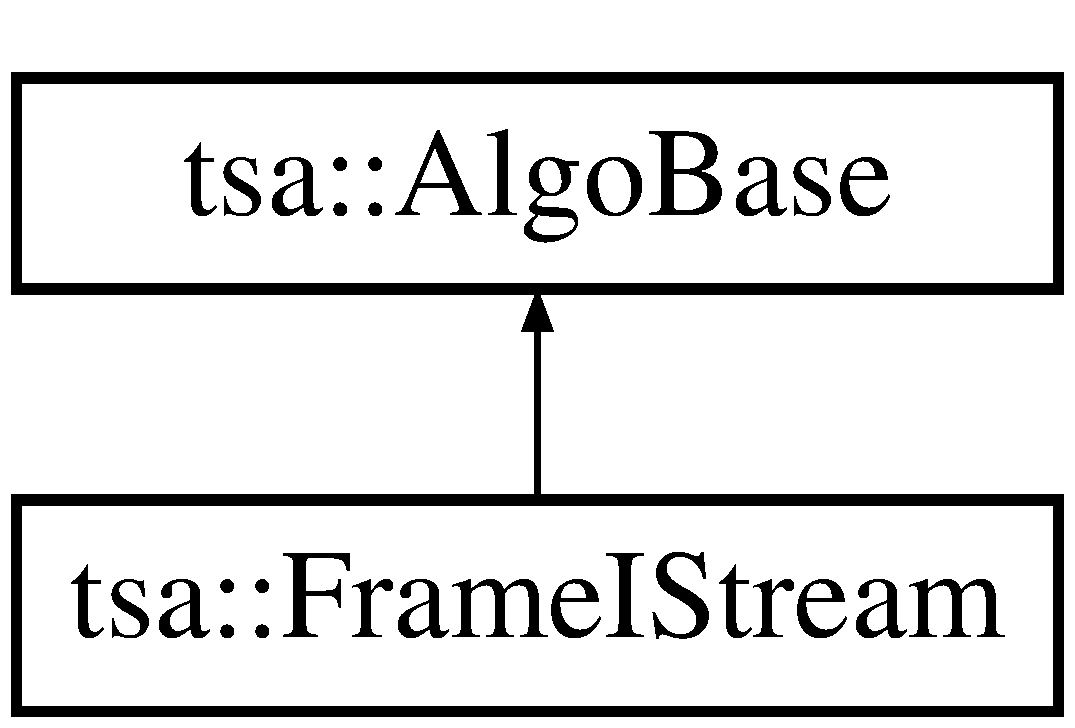
\includegraphics[height=2.000000cm]{classtsa_1_1_frame_i_stream}
\end{center}
\end{figure}
\subsection*{Public Member Functions}
\begin{DoxyCompactItemize}
\item 
\hyperlink{classtsa_1_1_frame_i_stream_a5bd1cb2479b947745f39121ba638d23f}{Frame\+I\+Stream} (const std\+::string \&file\+Name, const double \&Start\+Time)
\item 
\hyperlink{classtsa_1_1_frame_i_stream_a12f14bd9445709d3f03dcb122dc89889}{Frame\+I\+Stream} (const std\+::string \&file\+Name, const double \&Start\+Time, const double \&Time\+Length, const std\+::vector$<$ std\+::string $>$ \&channel\+Names)
\item 
\hyperlink{classtsa_1_1_frame_i_stream_a867c0e6a3cd0c2405c038026880d268d}{$\sim$\+Frame\+I\+Stream} ()
\end{DoxyCompactItemize}
\begin{Indent}\textbf{ Operations}\par
\begin{DoxyCompactItemize}
\item 
void \hyperlink{classtsa_1_1_frame_i_stream_a9c53d0d13f4fe78ce0eef01af69e3f22}{Init} ()
\item 
\hyperlink{classtsa_1_1_frame_i_stream}{Frame\+I\+Stream} \& \hyperlink{classtsa_1_1_frame_i_stream_ad2ad3c75a6448ce8ce8f119aee4609e5}{operator$>$$>$} (std\+::vector$<$ \hyperlink{namespacetsa_ac599574bcc094eda25613724b8f3ca9e}{Seq\+View\+Double} $>$ \&r\+Seq\+View)
\item 
\hyperlink{classtsa_1_1_frame_i_stream}{Frame\+I\+Stream} \& \hyperlink{classtsa_1_1_frame_i_stream_a1d57b62edf1783696b7c52120dad9e5a}{operator$>$$>$} (\hyperlink{namespacetsa_ac599574bcc094eda25613724b8f3ca9e}{Seq\+View\+Double} \&r\+Seq\+View)
\item 
void \hyperlink{classtsa_1_1_frame_i_stream_a66b4e5b136f07fc3044865908364c913}{Fill\+View} (\hyperlink{namespacetsa_ac599574bcc094eda25613724b8f3ca9e}{Seq\+View\+Double} \&r\+Seq\+View, double tstart, double tend)
\end{DoxyCompactItemize}
\end{Indent}
\begin{Indent}\textbf{ Getters}\par
\begin{DoxyCompactItemize}
\item 
std\+::string \hyperlink{classtsa_1_1_frame_i_stream_a3a199e1e8993581115311de3164550cc}{Get\+Info} (int gtime=0)
\item 
const std\+::string \& \hyperlink{classtsa_1_1_frame_i_stream_aa5e27458593c788665c737f40c445bf4}{Get\+File\+Name} (void) const
\item 
const std\+::vector$<$ std\+::string $>$ \& \hyperlink{classtsa_1_1_frame_i_stream_a0f65554481bf64cab44c7f5cbddb1987}{Get\+Channel\+Names} (void) const
\item 
double \hyperlink{classtsa_1_1_frame_i_stream_a88781ac3b80bddcca52e252f416009a6}{Get\+Start\+Time} (void) const
\item 
double \hyperlink{classtsa_1_1_frame_i_stream_a2b54726738d6155f6e4ccbae2b4a3f8f}{Get\+End\+Time} (void) const
\item 
double \hyperlink{classtsa_1_1_frame_i_stream_a02a205a02b70055814056216951476a6}{Get\+Sampling} (unsigned int cn) const
\item 
double \hyperlink{classtsa_1_1_frame_i_stream_aa9cae02ea01e99c39ba6a9da12fa8a21}{Get\+Time\+Length} ()
\item 
FrameH $\ast$ \hyperlink{classtsa_1_1_frame_i_stream_a7719f5fb6f7adc5b96555728489b5df6}{Get\+Frame} ()
\item 
struct Fr\+File $\ast$ \hyperlink{classtsa_1_1_frame_i_stream_a9ecf2c1985bf7578f70e0bef5ac993b3}{Get\+Frame\+File} ()
\item 
bool \hyperlink{classtsa_1_1_frame_i_stream_abdd07c781d107408f1b3e800e7fab42f}{Get\+Data\+Loss\+Flag} ()
\end{DoxyCompactItemize}
\end{Indent}
\begin{Indent}\textbf{ Setters}\par
\begin{DoxyCompactItemize}
\item 
void \hyperlink{classtsa_1_1_frame_i_stream_a5f23c61f80f232c70717dd2b021fae6d}{Set\+Channels} (const std\+::vector$<$ std\+::string $>$ \&channel\+Names)
\item 
void \hyperlink{classtsa_1_1_frame_i_stream_a8fb9dea502f55380a8a21e2976efa9b2}{Set\+Time\+Length} (double length)
\item 
void \hyperlink{classtsa_1_1_frame_i_stream_a1f12e9321856878c40266cd97890e3d4}{Reset\+Validation\+View} ()
\item 
void \hyperlink{classtsa_1_1_frame_i_stream_a89e7cd73df5fb44c8235166d8b9ccd12}{Set\+Validation\+View} (std\+::vector$<$ \hyperlink{namespacetsa_ac599574bcc094eda25613724b8f3ca9e}{Seq\+View\+Double} $>$ $\ast$r\+Validation\+View)
\item 
void \hyperlink{classtsa_1_1_frame_i_stream_a188c2351c1717037f955c959e61629ff}{Set\+Data\+Loss\+Flag} (bool status)
\item 
void \hyperlink{classtsa_1_1_frame_i_stream_a7a8b3b63fdc352215672bdbdcefdd295}{Add\+Exception} (const std\+::string \&msg, double miss\+\_\+start, double miss\+\_\+end, unsigned int channel)
\end{DoxyCompactItemize}
\end{Indent}
\subsection*{Private Member Functions}
\begin{DoxyCompactItemize}
\item 
\hyperlink{classtsa_1_1_channel_descriptor}{Channel\+Descriptor} $\ast$ \hyperlink{classtsa_1_1_frame_i_stream_a6a3a7e4523fed47c0055cb7ae1fd9435}{Create\+Channel\+Descriptor} (const std\+::string \&cname, unsigned int id)
\item 
bool \hyperlink{classtsa_1_1_frame_i_stream_af13e8a06bafa6e63bde6871d763425f1}{Data\+Required} ()
\item 
void \hyperlink{classtsa_1_1_frame_i_stream_a2f95f7fcf1e17f2d1b4a6b3dca976e76}{Get\+Data} ()
\end{DoxyCompactItemize}
\subsection*{Private Attributes}
\begin{DoxyCompactItemize}
\item 
double \hyperlink{classtsa_1_1_frame_i_stream_adad4100c6f0691cf47ca247b7b2f0fc6}{m\+Start\+Time}
\item 
double \hyperlink{classtsa_1_1_frame_i_stream_abd897050716a0879d2437a7e4f9f6b38}{m\+Time\+Length}
\item 
struct Fr\+File $\ast$ \hyperlink{classtsa_1_1_frame_i_stream_acee6c81e135c34abb9501753f8088a91}{mp\+Frame\+File}
\item 
FrameH $\ast$ \hyperlink{classtsa_1_1_frame_i_stream_a68ac0c21e3c23a219359e177623cf4e9}{mp\+Frame}
\item 
std\+::vector$<$ std\+::string $>$ \hyperlink{classtsa_1_1_frame_i_stream_a14bff233330be1d0f995551d55b8eb98}{m\+Channel\+Names}
\item 
std\+::string \hyperlink{classtsa_1_1_frame_i_stream_a888a976c4806d295c7ab6731459a0d90}{m\+File\+Name}
\item 
std\+::vector$<$ \hyperlink{classtsa_1_1_channel_descriptor}{Channel\+Descriptor} $\ast$ $>$ \hyperlink{classtsa_1_1_frame_i_stream_aef647c717912f7f4522d98fa967de2a0}{m\+Channel\+Descriptors}
\item 
std\+::vector$<$ \hyperlink{namespacetsa_ac599574bcc094eda25613724b8f3ca9e}{Seq\+View\+Double} $>$ $\ast$ \hyperlink{classtsa_1_1_frame_i_stream_a12d9c0c136ca288fc1fd64a660062494}{m\+Validation\+View}
\item 
bool \hyperlink{classtsa_1_1_frame_i_stream_aef23fdf187cda4ab4a3aaaa0a9ba59ee}{m\+Data\+Loss}
\item 
std\+::deque$<$ \hyperlink{classtsa_1_1missing__data}{missing\+\_\+data} $>$ \hyperlink{classtsa_1_1_frame_i_stream_ab0dfc2d31350678af1d0e1abe165ef65}{m\+Miss\+Exceptions}
\end{DoxyCompactItemize}


\subsection{Detailed Description}
A source of data taken from a Frame file. 

This class can be used to read data from a frame file. A set of channels can be specified, which are returned together.

Ser data\+:

Channel\+:\+Parameter\+:\+Frequency\+:Default 

Definition at line 536 of file Frame\+I\+Stream.\+hpp.



\subsection{Constructor \& Destructor Documentation}
\mbox{\Hypertarget{classtsa_1_1_frame_i_stream_a5bd1cb2479b947745f39121ba638d23f}\label{classtsa_1_1_frame_i_stream_a5bd1cb2479b947745f39121ba638d23f}} 
\index{tsa\+::\+Frame\+I\+Stream@{tsa\+::\+Frame\+I\+Stream}!Frame\+I\+Stream@{Frame\+I\+Stream}}
\index{Frame\+I\+Stream@{Frame\+I\+Stream}!tsa\+::\+Frame\+I\+Stream@{tsa\+::\+Frame\+I\+Stream}}
\subsubsection{\texorpdfstring{Frame\+I\+Stream()}{FrameIStream()}\hspace{0.1cm}{\footnotesize\ttfamily [1/2]}}
{\footnotesize\ttfamily tsa\+::\+Frame\+I\+Stream\+::\+Frame\+I\+Stream (\begin{DoxyParamCaption}\item[{const std\+::string \&}]{file\+Name,  }\item[{const double \&}]{Start\+Time }\end{DoxyParamCaption})}

Constructor


\begin{DoxyParams}{Parameters}
{\em file\+Name} & the name of the frame file (or a ffl file) \\
\hline
{\em Start\+Time} & start time of the data chunk we want \\
\hline
\end{DoxyParams}


Definition at line 590 of file Frame\+I\+Stream.\+cpp.

\mbox{\Hypertarget{classtsa_1_1_frame_i_stream_a12f14bd9445709d3f03dcb122dc89889}\label{classtsa_1_1_frame_i_stream_a12f14bd9445709d3f03dcb122dc89889}} 
\index{tsa\+::\+Frame\+I\+Stream@{tsa\+::\+Frame\+I\+Stream}!Frame\+I\+Stream@{Frame\+I\+Stream}}
\index{Frame\+I\+Stream@{Frame\+I\+Stream}!tsa\+::\+Frame\+I\+Stream@{tsa\+::\+Frame\+I\+Stream}}
\subsubsection{\texorpdfstring{Frame\+I\+Stream()}{FrameIStream()}\hspace{0.1cm}{\footnotesize\ttfamily [2/2]}}
{\footnotesize\ttfamily tsa\+::\+Frame\+I\+Stream\+::\+Frame\+I\+Stream (\begin{DoxyParamCaption}\item[{const std\+::string \&}]{file\+Name,  }\item[{const double \&}]{Start\+Time,  }\item[{const double \&}]{Time\+Length,  }\item[{const std\+::vector$<$ std\+::string $>$ \&}]{channel\+Names }\end{DoxyParamCaption})}

Constructor


\begin{DoxyParams}{Parameters}
{\em file\+Name} & the name of the frame file (or a ffl file) \\
\hline
{\em Start\+Time} & start time of the data chunk we want \\
\hline
{\em Time\+Length} & time length of requested data \\
\hline
{\em channel\+Names} & a list of channel\textquotesingle{}s names \\
\hline
\end{DoxyParams}


Definition at line 571 of file Frame\+I\+Stream.\+cpp.

\mbox{\Hypertarget{classtsa_1_1_frame_i_stream_a867c0e6a3cd0c2405c038026880d268d}\label{classtsa_1_1_frame_i_stream_a867c0e6a3cd0c2405c038026880d268d}} 
\index{tsa\+::\+Frame\+I\+Stream@{tsa\+::\+Frame\+I\+Stream}!````~Frame\+I\+Stream@{$\sim$\+Frame\+I\+Stream}}
\index{````~Frame\+I\+Stream@{$\sim$\+Frame\+I\+Stream}!tsa\+::\+Frame\+I\+Stream@{tsa\+::\+Frame\+I\+Stream}}
\subsubsection{\texorpdfstring{$\sim$\+Frame\+I\+Stream()}{~FrameIStream()}}
{\footnotesize\ttfamily tsa\+::\+Frame\+I\+Stream\+::$\sim$\+Frame\+I\+Stream (\begin{DoxyParamCaption}{ }\end{DoxyParamCaption})}

Destructor 

Definition at line 655 of file Frame\+I\+Stream.\+cpp.



\subsection{Member Function Documentation}
\mbox{\Hypertarget{classtsa_1_1_frame_i_stream_a7a8b3b63fdc352215672bdbdcefdd295}\label{classtsa_1_1_frame_i_stream_a7a8b3b63fdc352215672bdbdcefdd295}} 
\index{tsa\+::\+Frame\+I\+Stream@{tsa\+::\+Frame\+I\+Stream}!Add\+Exception@{Add\+Exception}}
\index{Add\+Exception@{Add\+Exception}!tsa\+::\+Frame\+I\+Stream@{tsa\+::\+Frame\+I\+Stream}}
\subsubsection{\texorpdfstring{Add\+Exception()}{AddException()}}
{\footnotesize\ttfamily void tsa\+::\+Frame\+I\+Stream\+::\+Add\+Exception (\begin{DoxyParamCaption}\item[{const std\+::string \&}]{msg,  }\item[{double}]{miss\+\_\+start,  }\item[{double}]{miss\+\_\+end,  }\item[{unsigned int}]{channel }\end{DoxyParamCaption})\hspace{0.3cm}{\ttfamily [inline]}}

Ad an exception to the set of data losses.


\begin{DoxyParams}{Parameters}
{\em msg} & exception textual message \\
\hline
{\em miss\+\_\+start} & start time for data loss \\
\hline
{\em miss\+\_\+end} & end time for data loss (excluded) \\
\hline
{\em channel} & channel where the data loss occurred \\
\hline
\end{DoxyParams}


Definition at line 739 of file Frame\+I\+Stream.\+hpp.

\mbox{\Hypertarget{classtsa_1_1_frame_i_stream_a6a3a7e4523fed47c0055cb7ae1fd9435}\label{classtsa_1_1_frame_i_stream_a6a3a7e4523fed47c0055cb7ae1fd9435}} 
\index{tsa\+::\+Frame\+I\+Stream@{tsa\+::\+Frame\+I\+Stream}!Create\+Channel\+Descriptor@{Create\+Channel\+Descriptor}}
\index{Create\+Channel\+Descriptor@{Create\+Channel\+Descriptor}!tsa\+::\+Frame\+I\+Stream@{tsa\+::\+Frame\+I\+Stream}}
\subsubsection{\texorpdfstring{Create\+Channel\+Descriptor()}{CreateChannelDescriptor()}}
{\footnotesize\ttfamily \hyperlink{classtsa_1_1_channel_descriptor}{Channel\+Descriptor} $\ast$ tsa\+::\+Frame\+I\+Stream\+::\+Create\+Channel\+Descriptor (\begin{DoxyParamCaption}\item[{const std\+::string \&}]{cname,  }\item[{unsigned int}]{id }\end{DoxyParamCaption})\hspace{0.3cm}{\ttfamily [private]}}

Create a new channel descriptor.


\begin{DoxyParams}{Parameters}
{\em cname} & the name of the requested channel descriptor \\
\hline
{\em id} & the index of the desired channel descriptor\\
\hline
\end{DoxyParams}
\begin{DoxyReturn}{Returns}
a pointer to the new channel descriptor structure, or null 
\end{DoxyReturn}


Definition at line 9 of file Frame\+I\+Stream.\+cpp.

\mbox{\Hypertarget{classtsa_1_1_frame_i_stream_af13e8a06bafa6e63bde6871d763425f1}\label{classtsa_1_1_frame_i_stream_af13e8a06bafa6e63bde6871d763425f1}} 
\index{tsa\+::\+Frame\+I\+Stream@{tsa\+::\+Frame\+I\+Stream}!Data\+Required@{Data\+Required}}
\index{Data\+Required@{Data\+Required}!tsa\+::\+Frame\+I\+Stream@{tsa\+::\+Frame\+I\+Stream}}
\subsubsection{\texorpdfstring{Data\+Required()}{DataRequired()}}
{\footnotesize\ttfamily bool tsa\+::\+Frame\+I\+Stream\+::\+Data\+Required (\begin{DoxyParamCaption}{ }\end{DoxyParamCaption})\hspace{0.3cm}{\ttfamily [private]}}

Test if some data are required.

\begin{DoxyReturn}{Returns}
true if soem data are required 
\end{DoxyReturn}


Definition at line 823 of file Frame\+I\+Stream.\+cpp.

\mbox{\Hypertarget{classtsa_1_1_frame_i_stream_a66b4e5b136f07fc3044865908364c913}\label{classtsa_1_1_frame_i_stream_a66b4e5b136f07fc3044865908364c913}} 
\index{tsa\+::\+Frame\+I\+Stream@{tsa\+::\+Frame\+I\+Stream}!Fill\+View@{Fill\+View}}
\index{Fill\+View@{Fill\+View}!tsa\+::\+Frame\+I\+Stream@{tsa\+::\+Frame\+I\+Stream}}
\subsubsection{\texorpdfstring{Fill\+View()}{FillView()}}
{\footnotesize\ttfamily void tsa\+::\+Frame\+I\+Stream\+::\+Fill\+View (\begin{DoxyParamCaption}\item[{\hyperlink{namespacetsa_ac599574bcc094eda25613724b8f3ca9e}{Seq\+View\+Double} \&}]{r\+Seq\+View,  }\item[{double}]{tstart,  }\item[{double}]{tend }\end{DoxyParamCaption})}



Definition at line 847 of file Frame\+I\+Stream.\+cpp.

\mbox{\Hypertarget{classtsa_1_1_frame_i_stream_a0f65554481bf64cab44c7f5cbddb1987}\label{classtsa_1_1_frame_i_stream_a0f65554481bf64cab44c7f5cbddb1987}} 
\index{tsa\+::\+Frame\+I\+Stream@{tsa\+::\+Frame\+I\+Stream}!Get\+Channel\+Names@{Get\+Channel\+Names}}
\index{Get\+Channel\+Names@{Get\+Channel\+Names}!tsa\+::\+Frame\+I\+Stream@{tsa\+::\+Frame\+I\+Stream}}
\subsubsection{\texorpdfstring{Get\+Channel\+Names()}{GetChannelNames()}}
{\footnotesize\ttfamily const std\+::vector$<$ std\+::string $>$ \& tsa\+::\+Frame\+I\+Stream\+::\+Get\+Channel\+Names (\begin{DoxyParamCaption}\item[{void}]{ }\end{DoxyParamCaption}) const}

Get the list of the channel\textquotesingle{}s names.

\begin{DoxyReturn}{Returns}
a list of channel\textquotesingle{}s names 
\end{DoxyReturn}


Definition at line 757 of file Frame\+I\+Stream.\+cpp.

\mbox{\Hypertarget{classtsa_1_1_frame_i_stream_a2f95f7fcf1e17f2d1b4a6b3dca976e76}\label{classtsa_1_1_frame_i_stream_a2f95f7fcf1e17f2d1b4a6b3dca976e76}} 
\index{tsa\+::\+Frame\+I\+Stream@{tsa\+::\+Frame\+I\+Stream}!Get\+Data@{Get\+Data}}
\index{Get\+Data@{Get\+Data}!tsa\+::\+Frame\+I\+Stream@{tsa\+::\+Frame\+I\+Stream}}
\subsubsection{\texorpdfstring{Get\+Data()}{GetData()}}
{\footnotesize\ttfamily void tsa\+::\+Frame\+I\+Stream\+::\+Get\+Data (\begin{DoxyParamCaption}{ }\end{DoxyParamCaption})\hspace{0.3cm}{\ttfamily [private]}}

Get new data from the file 

Definition at line 805 of file Frame\+I\+Stream.\+cpp.

\mbox{\Hypertarget{classtsa_1_1_frame_i_stream_abdd07c781d107408f1b3e800e7fab42f}\label{classtsa_1_1_frame_i_stream_abdd07c781d107408f1b3e800e7fab42f}} 
\index{tsa\+::\+Frame\+I\+Stream@{tsa\+::\+Frame\+I\+Stream}!Get\+Data\+Loss\+Flag@{Get\+Data\+Loss\+Flag}}
\index{Get\+Data\+Loss\+Flag@{Get\+Data\+Loss\+Flag}!tsa\+::\+Frame\+I\+Stream@{tsa\+::\+Frame\+I\+Stream}}
\subsubsection{\texorpdfstring{Get\+Data\+Loss\+Flag()}{GetDataLossFlag()}}
{\footnotesize\ttfamily bool tsa\+::\+Frame\+I\+Stream\+::\+Get\+Data\+Loss\+Flag (\begin{DoxyParamCaption}{ }\end{DoxyParamCaption})\hspace{0.3cm}{\ttfamily [inline]}}

Get the value of the data loss flag. It is true if a data loss event is occurred.

\begin{DoxyReturn}{Returns}
the data loss flag value 
\end{DoxyReturn}


Definition at line 684 of file Frame\+I\+Stream.\+hpp.

\mbox{\Hypertarget{classtsa_1_1_frame_i_stream_a2b54726738d6155f6e4ccbae2b4a3f8f}\label{classtsa_1_1_frame_i_stream_a2b54726738d6155f6e4ccbae2b4a3f8f}} 
\index{tsa\+::\+Frame\+I\+Stream@{tsa\+::\+Frame\+I\+Stream}!Get\+End\+Time@{Get\+End\+Time}}
\index{Get\+End\+Time@{Get\+End\+Time}!tsa\+::\+Frame\+I\+Stream@{tsa\+::\+Frame\+I\+Stream}}
\subsubsection{\texorpdfstring{Get\+End\+Time()}{GetEndTime()}}
{\footnotesize\ttfamily double tsa\+::\+Frame\+I\+Stream\+::\+Get\+End\+Time (\begin{DoxyParamCaption}\item[{void}]{ }\end{DoxyParamCaption}) const}

Get the actual end time, which is the end time of the next data chunk that will be read.

\begin{DoxyReturn}{Returns}
the actual end time 
\end{DoxyReturn}


Definition at line 765 of file Frame\+I\+Stream.\+cpp.

\mbox{\Hypertarget{classtsa_1_1_frame_i_stream_aa5e27458593c788665c737f40c445bf4}\label{classtsa_1_1_frame_i_stream_aa5e27458593c788665c737f40c445bf4}} 
\index{tsa\+::\+Frame\+I\+Stream@{tsa\+::\+Frame\+I\+Stream}!Get\+File\+Name@{Get\+File\+Name}}
\index{Get\+File\+Name@{Get\+File\+Name}!tsa\+::\+Frame\+I\+Stream@{tsa\+::\+Frame\+I\+Stream}}
\subsubsection{\texorpdfstring{Get\+File\+Name()}{GetFileName()}}
{\footnotesize\ttfamily const std\+::string \& tsa\+::\+Frame\+I\+Stream\+::\+Get\+File\+Name (\begin{DoxyParamCaption}\item[{void}]{ }\end{DoxyParamCaption}) const}

Get the file name of the frame file used.

\begin{DoxyReturn}{Returns}
the file name of the frame file 
\end{DoxyReturn}


Definition at line 753 of file Frame\+I\+Stream.\+cpp.

\mbox{\Hypertarget{classtsa_1_1_frame_i_stream_a7719f5fb6f7adc5b96555728489b5df6}\label{classtsa_1_1_frame_i_stream_a7719f5fb6f7adc5b96555728489b5df6}} 
\index{tsa\+::\+Frame\+I\+Stream@{tsa\+::\+Frame\+I\+Stream}!Get\+Frame@{Get\+Frame}}
\index{Get\+Frame@{Get\+Frame}!tsa\+::\+Frame\+I\+Stream@{tsa\+::\+Frame\+I\+Stream}}
\subsubsection{\texorpdfstring{Get\+Frame()}{GetFrame()}}
{\footnotesize\ttfamily FrameH$\ast$ tsa\+::\+Frame\+I\+Stream\+::\+Get\+Frame (\begin{DoxyParamCaption}{ }\end{DoxyParamCaption})\hspace{0.3cm}{\ttfamily [inline]}}

Get a pointer to the current FrameH structure.

\begin{DoxyReturn}{Returns}
a pointer to the current FrameH 
\end{DoxyReturn}


Definition at line 670 of file Frame\+I\+Stream.\+hpp.

\mbox{\Hypertarget{classtsa_1_1_frame_i_stream_a9ecf2c1985bf7578f70e0bef5ac993b3}\label{classtsa_1_1_frame_i_stream_a9ecf2c1985bf7578f70e0bef5ac993b3}} 
\index{tsa\+::\+Frame\+I\+Stream@{tsa\+::\+Frame\+I\+Stream}!Get\+Frame\+File@{Get\+Frame\+File}}
\index{Get\+Frame\+File@{Get\+Frame\+File}!tsa\+::\+Frame\+I\+Stream@{tsa\+::\+Frame\+I\+Stream}}
\subsubsection{\texorpdfstring{Get\+Frame\+File()}{GetFrameFile()}}
{\footnotesize\ttfamily struct Fr\+File$\ast$ tsa\+::\+Frame\+I\+Stream\+::\+Get\+Frame\+File (\begin{DoxyParamCaption}{ }\end{DoxyParamCaption})\hspace{0.3cm}{\ttfamily [inline]}}



Definition at line 674 of file Frame\+I\+Stream.\+hpp.

\mbox{\Hypertarget{classtsa_1_1_frame_i_stream_a3a199e1e8993581115311de3164550cc}\label{classtsa_1_1_frame_i_stream_a3a199e1e8993581115311de3164550cc}} 
\index{tsa\+::\+Frame\+I\+Stream@{tsa\+::\+Frame\+I\+Stream}!Get\+Info@{Get\+Info}}
\index{Get\+Info@{Get\+Info}!tsa\+::\+Frame\+I\+Stream@{tsa\+::\+Frame\+I\+Stream}}
\subsubsection{\texorpdfstring{Get\+Info()}{GetInfo()}}
{\footnotesize\ttfamily std\+::string tsa\+::\+Frame\+I\+Stream\+::\+Get\+Info (\begin{DoxyParamCaption}\item[{int}]{gtime = {\ttfamily 0} }\end{DoxyParamCaption})}



Definition at line 664 of file Frame\+I\+Stream.\+cpp.

\mbox{\Hypertarget{classtsa_1_1_frame_i_stream_a02a205a02b70055814056216951476a6}\label{classtsa_1_1_frame_i_stream_a02a205a02b70055814056216951476a6}} 
\index{tsa\+::\+Frame\+I\+Stream@{tsa\+::\+Frame\+I\+Stream}!Get\+Sampling@{Get\+Sampling}}
\index{Get\+Sampling@{Get\+Sampling}!tsa\+::\+Frame\+I\+Stream@{tsa\+::\+Frame\+I\+Stream}}
\subsubsection{\texorpdfstring{Get\+Sampling()}{GetSampling()}}
{\footnotesize\ttfamily double tsa\+::\+Frame\+I\+Stream\+::\+Get\+Sampling (\begin{DoxyParamCaption}\item[{unsigned int}]{cn }\end{DoxyParamCaption}) const}

Get the sampling time of a channel


\begin{DoxyParams}{Parameters}
{\em cname} & the channel\textquotesingle{}s name\\
\hline
\end{DoxyParams}
\begin{DoxyReturn}{Returns}
the channel\textquotesingle{}s sampling time 
\end{DoxyReturn}


Definition at line 769 of file Frame\+I\+Stream.\+cpp.

\mbox{\Hypertarget{classtsa_1_1_frame_i_stream_a88781ac3b80bddcca52e252f416009a6}\label{classtsa_1_1_frame_i_stream_a88781ac3b80bddcca52e252f416009a6}} 
\index{tsa\+::\+Frame\+I\+Stream@{tsa\+::\+Frame\+I\+Stream}!Get\+Start\+Time@{Get\+Start\+Time}}
\index{Get\+Start\+Time@{Get\+Start\+Time}!tsa\+::\+Frame\+I\+Stream@{tsa\+::\+Frame\+I\+Stream}}
\subsubsection{\texorpdfstring{Get\+Start\+Time()}{GetStartTime()}}
{\footnotesize\ttfamily double tsa\+::\+Frame\+I\+Stream\+::\+Get\+Start\+Time (\begin{DoxyParamCaption}\item[{void}]{ }\end{DoxyParamCaption}) const}

Get the actual start time, which is the start time of the next data chunk that will be read.

\begin{DoxyReturn}{Returns}
the actual start time 
\end{DoxyReturn}


Definition at line 761 of file Frame\+I\+Stream.\+cpp.

\mbox{\Hypertarget{classtsa_1_1_frame_i_stream_aa9cae02ea01e99c39ba6a9da12fa8a21}\label{classtsa_1_1_frame_i_stream_aa9cae02ea01e99c39ba6a9da12fa8a21}} 
\index{tsa\+::\+Frame\+I\+Stream@{tsa\+::\+Frame\+I\+Stream}!Get\+Time\+Length@{Get\+Time\+Length}}
\index{Get\+Time\+Length@{Get\+Time\+Length}!tsa\+::\+Frame\+I\+Stream@{tsa\+::\+Frame\+I\+Stream}}
\subsubsection{\texorpdfstring{Get\+Time\+Length()}{GetTimeLength()}}
{\footnotesize\ttfamily double tsa\+::\+Frame\+I\+Stream\+::\+Get\+Time\+Length (\begin{DoxyParamCaption}{ }\end{DoxyParamCaption})\hspace{0.3cm}{\ttfamily [inline]}}

Get the time duration of the next data chunk that will be read.

\begin{DoxyReturn}{Returns}
the actual time duration. 
\end{DoxyReturn}


Definition at line 660 of file Frame\+I\+Stream.\+hpp.

\mbox{\Hypertarget{classtsa_1_1_frame_i_stream_a9c53d0d13f4fe78ce0eef01af69e3f22}\label{classtsa_1_1_frame_i_stream_a9c53d0d13f4fe78ce0eef01af69e3f22}} 
\index{tsa\+::\+Frame\+I\+Stream@{tsa\+::\+Frame\+I\+Stream}!Init@{Init}}
\index{Init@{Init}!tsa\+::\+Frame\+I\+Stream@{tsa\+::\+Frame\+I\+Stream}}
\subsubsection{\texorpdfstring{Init()}{Init()}}
{\footnotesize\ttfamily void tsa\+::\+Frame\+I\+Stream\+::\+Init (\begin{DoxyParamCaption}{ }\end{DoxyParamCaption})}



Definition at line 606 of file Frame\+I\+Stream.\+cpp.

\mbox{\Hypertarget{classtsa_1_1_frame_i_stream_ad2ad3c75a6448ce8ce8f119aee4609e5}\label{classtsa_1_1_frame_i_stream_ad2ad3c75a6448ce8ce8f119aee4609e5}} 
\index{tsa\+::\+Frame\+I\+Stream@{tsa\+::\+Frame\+I\+Stream}!operator$>$$>$@{operator$>$$>$}}
\index{operator$>$$>$@{operator$>$$>$}!tsa\+::\+Frame\+I\+Stream@{tsa\+::\+Frame\+I\+Stream}}
\subsubsection{\texorpdfstring{operator$>$$>$()}{operator>>()}\hspace{0.1cm}{\footnotesize\ttfamily [1/2]}}
{\footnotesize\ttfamily \hyperlink{classtsa_1_1_frame_i_stream}{Frame\+I\+Stream} \& tsa\+::\+Frame\+I\+Stream\+::operator$>$$>$ (\begin{DoxyParamCaption}\item[{std\+::vector$<$ \hyperlink{namespacetsa_ac599574bcc094eda25613724b8f3ca9e}{Seq\+View\+Double} $>$ \&}]{r\+Seq\+View }\end{DoxyParamCaption})}

Read data from the frame file.


\begin{DoxyParams}{Parameters}
{\em r\+Seq\+View} & A list of time views to fill with data. Each view contain a single channel.\\
\hline
\end{DoxyParams}
\begin{DoxyReturn}{Returns}
a reference to the instance of the class 
\end{DoxyReturn}


Definition at line 716 of file Frame\+I\+Stream.\+cpp.

\mbox{\Hypertarget{classtsa_1_1_frame_i_stream_a1d57b62edf1783696b7c52120dad9e5a}\label{classtsa_1_1_frame_i_stream_a1d57b62edf1783696b7c52120dad9e5a}} 
\index{tsa\+::\+Frame\+I\+Stream@{tsa\+::\+Frame\+I\+Stream}!operator$>$$>$@{operator$>$$>$}}
\index{operator$>$$>$@{operator$>$$>$}!tsa\+::\+Frame\+I\+Stream@{tsa\+::\+Frame\+I\+Stream}}
\subsubsection{\texorpdfstring{operator$>$$>$()}{operator>>()}\hspace{0.1cm}{\footnotesize\ttfamily [2/2]}}
{\footnotesize\ttfamily \hyperlink{classtsa_1_1_frame_i_stream}{Frame\+I\+Stream} \& tsa\+::\+Frame\+I\+Stream\+::operator$>$$>$ (\begin{DoxyParamCaption}\item[{\hyperlink{namespacetsa_ac599574bcc094eda25613724b8f3ca9e}{Seq\+View\+Double} \&}]{r\+Seq\+View }\end{DoxyParamCaption})}

Read data from the frame file.


\begin{DoxyParams}{Parameters}
{\em r\+Seq\+View} & A list a time view to fill with data. It contains a single channel.\\
\hline
\end{DoxyParams}
\begin{DoxyReturn}{Returns}
a reference to the instance of the class 
\end{DoxyReturn}


Definition at line 688 of file Frame\+I\+Stream.\+cpp.

\mbox{\Hypertarget{classtsa_1_1_frame_i_stream_a1f12e9321856878c40266cd97890e3d4}\label{classtsa_1_1_frame_i_stream_a1f12e9321856878c40266cd97890e3d4}} 
\index{tsa\+::\+Frame\+I\+Stream@{tsa\+::\+Frame\+I\+Stream}!Reset\+Validation\+View@{Reset\+Validation\+View}}
\index{Reset\+Validation\+View@{Reset\+Validation\+View}!tsa\+::\+Frame\+I\+Stream@{tsa\+::\+Frame\+I\+Stream}}
\subsubsection{\texorpdfstring{Reset\+Validation\+View()}{ResetValidationView()}}
{\footnotesize\ttfamily void tsa\+::\+Frame\+I\+Stream\+::\+Reset\+Validation\+View (\begin{DoxyParamCaption}{ }\end{DoxyParamCaption})}

Set to zero the validation view. No validation data are written. 

Definition at line 839 of file Frame\+I\+Stream.\+cpp.

\mbox{\Hypertarget{classtsa_1_1_frame_i_stream_a5f23c61f80f232c70717dd2b021fae6d}\label{classtsa_1_1_frame_i_stream_a5f23c61f80f232c70717dd2b021fae6d}} 
\index{tsa\+::\+Frame\+I\+Stream@{tsa\+::\+Frame\+I\+Stream}!Set\+Channels@{Set\+Channels}}
\index{Set\+Channels@{Set\+Channels}!tsa\+::\+Frame\+I\+Stream@{tsa\+::\+Frame\+I\+Stream}}
\subsubsection{\texorpdfstring{Set\+Channels()}{SetChannels()}}
{\footnotesize\ttfamily void tsa\+::\+Frame\+I\+Stream\+::\+Set\+Channels (\begin{DoxyParamCaption}\item[{const std\+::vector$<$ std\+::string $>$ \&}]{channel\+Names }\end{DoxyParamCaption})}

Set the channels which should be opened


\begin{DoxyParams}{Parameters}
{\em channel\+Names} & vector of names for the channels \\
\hline
\end{DoxyParams}


Definition at line 773 of file Frame\+I\+Stream.\+cpp.

\mbox{\Hypertarget{classtsa_1_1_frame_i_stream_a188c2351c1717037f955c959e61629ff}\label{classtsa_1_1_frame_i_stream_a188c2351c1717037f955c959e61629ff}} 
\index{tsa\+::\+Frame\+I\+Stream@{tsa\+::\+Frame\+I\+Stream}!Set\+Data\+Loss\+Flag@{Set\+Data\+Loss\+Flag}}
\index{Set\+Data\+Loss\+Flag@{Set\+Data\+Loss\+Flag}!tsa\+::\+Frame\+I\+Stream@{tsa\+::\+Frame\+I\+Stream}}
\subsubsection{\texorpdfstring{Set\+Data\+Loss\+Flag()}{SetDataLossFlag()}}
{\footnotesize\ttfamily void tsa\+::\+Frame\+I\+Stream\+::\+Set\+Data\+Loss\+Flag (\begin{DoxyParamCaption}\item[{bool}]{status }\end{DoxyParamCaption})\hspace{0.3cm}{\ttfamily [inline]}}

Set the value of the data loss flag.


\begin{DoxyParams}{Parameters}
{\em status} & new value of the data loss flag \\
\hline
\end{DoxyParams}


Definition at line 727 of file Frame\+I\+Stream.\+hpp.

\mbox{\Hypertarget{classtsa_1_1_frame_i_stream_a8fb9dea502f55380a8a21e2976efa9b2}\label{classtsa_1_1_frame_i_stream_a8fb9dea502f55380a8a21e2976efa9b2}} 
\index{tsa\+::\+Frame\+I\+Stream@{tsa\+::\+Frame\+I\+Stream}!Set\+Time\+Length@{Set\+Time\+Length}}
\index{Set\+Time\+Length@{Set\+Time\+Length}!tsa\+::\+Frame\+I\+Stream@{tsa\+::\+Frame\+I\+Stream}}
\subsubsection{\texorpdfstring{Set\+Time\+Length()}{SetTimeLength()}}
{\footnotesize\ttfamily void tsa\+::\+Frame\+I\+Stream\+::\+Set\+Time\+Length (\begin{DoxyParamCaption}\item[{double}]{length }\end{DoxyParamCaption})}

Set the length of the data buffer that will be returned from now on 
\begin{DoxyParams}{Parameters}
{\em length} & the new length \\
\hline
\end{DoxyParams}


Definition at line 801 of file Frame\+I\+Stream.\+cpp.

\mbox{\Hypertarget{classtsa_1_1_frame_i_stream_a89e7cd73df5fb44c8235166d8b9ccd12}\label{classtsa_1_1_frame_i_stream_a89e7cd73df5fb44c8235166d8b9ccd12}} 
\index{tsa\+::\+Frame\+I\+Stream@{tsa\+::\+Frame\+I\+Stream}!Set\+Validation\+View@{Set\+Validation\+View}}
\index{Set\+Validation\+View@{Set\+Validation\+View}!tsa\+::\+Frame\+I\+Stream@{tsa\+::\+Frame\+I\+Stream}}
\subsubsection{\texorpdfstring{Set\+Validation\+View()}{SetValidationView()}}
{\footnotesize\ttfamily void tsa\+::\+Frame\+I\+Stream\+::\+Set\+Validation\+View (\begin{DoxyParamCaption}\item[{std\+::vector$<$ \hyperlink{namespacetsa_ac599574bcc094eda25613724b8f3ca9e}{Seq\+View\+Double} $>$ $\ast$}]{r\+Validation\+View }\end{DoxyParamCaption})}

Set the current validation view. From now on the validation data are written on the given views every time some data is read.


\begin{DoxyParams}{Parameters}
{\em r\+Validation\+View} & pointer to a vector of validation views \\
\hline
\end{DoxyParams}


Definition at line 843 of file Frame\+I\+Stream.\+cpp.



\subsection{Member Data Documentation}
\mbox{\Hypertarget{classtsa_1_1_frame_i_stream_aef647c717912f7f4522d98fa967de2a0}\label{classtsa_1_1_frame_i_stream_aef647c717912f7f4522d98fa967de2a0}} 
\index{tsa\+::\+Frame\+I\+Stream@{tsa\+::\+Frame\+I\+Stream}!m\+Channel\+Descriptors@{m\+Channel\+Descriptors}}
\index{m\+Channel\+Descriptors@{m\+Channel\+Descriptors}!tsa\+::\+Frame\+I\+Stream@{tsa\+::\+Frame\+I\+Stream}}
\subsubsection{\texorpdfstring{m\+Channel\+Descriptors}{mChannelDescriptors}}
{\footnotesize\ttfamily std\+::vector$<$\hyperlink{classtsa_1_1_channel_descriptor}{Channel\+Descriptor}$\ast$$>$ tsa\+::\+Frame\+I\+Stream\+::m\+Channel\+Descriptors\hspace{0.3cm}{\ttfamily [private]}}

list of channel descriptor 

Definition at line 780 of file Frame\+I\+Stream.\+hpp.

\mbox{\Hypertarget{classtsa_1_1_frame_i_stream_a14bff233330be1d0f995551d55b8eb98}\label{classtsa_1_1_frame_i_stream_a14bff233330be1d0f995551d55b8eb98}} 
\index{tsa\+::\+Frame\+I\+Stream@{tsa\+::\+Frame\+I\+Stream}!m\+Channel\+Names@{m\+Channel\+Names}}
\index{m\+Channel\+Names@{m\+Channel\+Names}!tsa\+::\+Frame\+I\+Stream@{tsa\+::\+Frame\+I\+Stream}}
\subsubsection{\texorpdfstring{m\+Channel\+Names}{mChannelNames}}
{\footnotesize\ttfamily std\+::vector$<$std\+::string$>$ tsa\+::\+Frame\+I\+Stream\+::m\+Channel\+Names\hspace{0.3cm}{\ttfamily [private]}}

The list of channel names 

Definition at line 778 of file Frame\+I\+Stream.\+hpp.

\mbox{\Hypertarget{classtsa_1_1_frame_i_stream_aef23fdf187cda4ab4a3aaaa0a9ba59ee}\label{classtsa_1_1_frame_i_stream_aef23fdf187cda4ab4a3aaaa0a9ba59ee}} 
\index{tsa\+::\+Frame\+I\+Stream@{tsa\+::\+Frame\+I\+Stream}!m\+Data\+Loss@{m\+Data\+Loss}}
\index{m\+Data\+Loss@{m\+Data\+Loss}!tsa\+::\+Frame\+I\+Stream@{tsa\+::\+Frame\+I\+Stream}}
\subsubsection{\texorpdfstring{m\+Data\+Loss}{mDataLoss}}
{\footnotesize\ttfamily bool tsa\+::\+Frame\+I\+Stream\+::m\+Data\+Loss\hspace{0.3cm}{\ttfamily [private]}}

Data loss flag 

Definition at line 782 of file Frame\+I\+Stream.\+hpp.

\mbox{\Hypertarget{classtsa_1_1_frame_i_stream_a888a976c4806d295c7ab6731459a0d90}\label{classtsa_1_1_frame_i_stream_a888a976c4806d295c7ab6731459a0d90}} 
\index{tsa\+::\+Frame\+I\+Stream@{tsa\+::\+Frame\+I\+Stream}!m\+File\+Name@{m\+File\+Name}}
\index{m\+File\+Name@{m\+File\+Name}!tsa\+::\+Frame\+I\+Stream@{tsa\+::\+Frame\+I\+Stream}}
\subsubsection{\texorpdfstring{m\+File\+Name}{mFileName}}
{\footnotesize\ttfamily std\+::string tsa\+::\+Frame\+I\+Stream\+::m\+File\+Name\hspace{0.3cm}{\ttfamily [private]}}

The file name 

Definition at line 779 of file Frame\+I\+Stream.\+hpp.

\mbox{\Hypertarget{classtsa_1_1_frame_i_stream_ab0dfc2d31350678af1d0e1abe165ef65}\label{classtsa_1_1_frame_i_stream_ab0dfc2d31350678af1d0e1abe165ef65}} 
\index{tsa\+::\+Frame\+I\+Stream@{tsa\+::\+Frame\+I\+Stream}!m\+Miss\+Exceptions@{m\+Miss\+Exceptions}}
\index{m\+Miss\+Exceptions@{m\+Miss\+Exceptions}!tsa\+::\+Frame\+I\+Stream@{tsa\+::\+Frame\+I\+Stream}}
\subsubsection{\texorpdfstring{m\+Miss\+Exceptions}{mMissExceptions}}
{\footnotesize\ttfamily std\+::deque$<$\hyperlink{classtsa_1_1missing__data}{missing\+\_\+data}$>$ tsa\+::\+Frame\+I\+Stream\+::m\+Miss\+Exceptions\hspace{0.3cm}{\ttfamily [private]}}

Set of data loss exception 

Definition at line 783 of file Frame\+I\+Stream.\+hpp.

\mbox{\Hypertarget{classtsa_1_1_frame_i_stream_a68ac0c21e3c23a219359e177623cf4e9}\label{classtsa_1_1_frame_i_stream_a68ac0c21e3c23a219359e177623cf4e9}} 
\index{tsa\+::\+Frame\+I\+Stream@{tsa\+::\+Frame\+I\+Stream}!mp\+Frame@{mp\+Frame}}
\index{mp\+Frame@{mp\+Frame}!tsa\+::\+Frame\+I\+Stream@{tsa\+::\+Frame\+I\+Stream}}
\subsubsection{\texorpdfstring{mp\+Frame}{mpFrame}}
{\footnotesize\ttfamily FrameH$\ast$ tsa\+::\+Frame\+I\+Stream\+::mp\+Frame\hspace{0.3cm}{\ttfamily [private]}}

The current FrameH structure 

Definition at line 777 of file Frame\+I\+Stream.\+hpp.

\mbox{\Hypertarget{classtsa_1_1_frame_i_stream_acee6c81e135c34abb9501753f8088a91}\label{classtsa_1_1_frame_i_stream_acee6c81e135c34abb9501753f8088a91}} 
\index{tsa\+::\+Frame\+I\+Stream@{tsa\+::\+Frame\+I\+Stream}!mp\+Frame\+File@{mp\+Frame\+File}}
\index{mp\+Frame\+File@{mp\+Frame\+File}!tsa\+::\+Frame\+I\+Stream@{tsa\+::\+Frame\+I\+Stream}}
\subsubsection{\texorpdfstring{mp\+Frame\+File}{mpFrameFile}}
{\footnotesize\ttfamily struct Fr\+File$\ast$ tsa\+::\+Frame\+I\+Stream\+::mp\+Frame\+File\hspace{0.3cm}{\ttfamily [private]}}

The current frame file 

Definition at line 776 of file Frame\+I\+Stream.\+hpp.

\mbox{\Hypertarget{classtsa_1_1_frame_i_stream_adad4100c6f0691cf47ca247b7b2f0fc6}\label{classtsa_1_1_frame_i_stream_adad4100c6f0691cf47ca247b7b2f0fc6}} 
\index{tsa\+::\+Frame\+I\+Stream@{tsa\+::\+Frame\+I\+Stream}!m\+Start\+Time@{m\+Start\+Time}}
\index{m\+Start\+Time@{m\+Start\+Time}!tsa\+::\+Frame\+I\+Stream@{tsa\+::\+Frame\+I\+Stream}}
\subsubsection{\texorpdfstring{m\+Start\+Time}{mStartTime}}
{\footnotesize\ttfamily double tsa\+::\+Frame\+I\+Stream\+::m\+Start\+Time\hspace{0.3cm}{\ttfamily [private]}}

Start time for the data queue 

Definition at line 774 of file Frame\+I\+Stream.\+hpp.

\mbox{\Hypertarget{classtsa_1_1_frame_i_stream_abd897050716a0879d2437a7e4f9f6b38}\label{classtsa_1_1_frame_i_stream_abd897050716a0879d2437a7e4f9f6b38}} 
\index{tsa\+::\+Frame\+I\+Stream@{tsa\+::\+Frame\+I\+Stream}!m\+Time\+Length@{m\+Time\+Length}}
\index{m\+Time\+Length@{m\+Time\+Length}!tsa\+::\+Frame\+I\+Stream@{tsa\+::\+Frame\+I\+Stream}}
\subsubsection{\texorpdfstring{m\+Time\+Length}{mTimeLength}}
{\footnotesize\ttfamily double tsa\+::\+Frame\+I\+Stream\+::m\+Time\+Length\hspace{0.3cm}{\ttfamily [private]}}

Time length of the data given at each request 

Definition at line 775 of file Frame\+I\+Stream.\+hpp.

\mbox{\Hypertarget{classtsa_1_1_frame_i_stream_a12d9c0c136ca288fc1fd64a660062494}\label{classtsa_1_1_frame_i_stream_a12d9c0c136ca288fc1fd64a660062494}} 
\index{tsa\+::\+Frame\+I\+Stream@{tsa\+::\+Frame\+I\+Stream}!m\+Validation\+View@{m\+Validation\+View}}
\index{m\+Validation\+View@{m\+Validation\+View}!tsa\+::\+Frame\+I\+Stream@{tsa\+::\+Frame\+I\+Stream}}
\subsubsection{\texorpdfstring{m\+Validation\+View}{mValidationView}}
{\footnotesize\ttfamily std\+::vector$<$\hyperlink{namespacetsa_ac599574bcc094eda25613724b8f3ca9e}{Seq\+View\+Double}$>$$\ast$ tsa\+::\+Frame\+I\+Stream\+::m\+Validation\+View\hspace{0.3cm}{\ttfamily [private]}}

Pointer to the validation views 

Definition at line 781 of file Frame\+I\+Stream.\+hpp.



The documentation for this class was generated from the following files\+:\begin{DoxyCompactItemize}
\item 
/home/filip/\+Ph\+D/\+W\+D\+F\+Pipe\+\_\+test/p4\+T\+S\+A/include/\hyperlink{_frame_i_stream_8hpp}{Frame\+I\+Stream.\+hpp}\item 
/home/filip/\+Ph\+D/\+W\+D\+F\+Pipe\+\_\+test/p4\+T\+S\+A/src/\hyperlink{_frame_i_stream_8cpp}{Frame\+I\+Stream.\+cpp}\end{DoxyCompactItemize}

\hypertarget{struct_f_u_n_c_t_i_o_n_p_a_r_s_e_r_t_y_p_e_s_1_1_func_definition}{}\section{F\+U\+N\+C\+T\+I\+O\+N\+P\+A\+R\+S\+E\+R\+T\+Y\+P\+ES\+:\+:Func\+Definition Struct Reference}
\label{struct_f_u_n_c_t_i_o_n_p_a_r_s_e_r_t_y_p_e_s_1_1_func_definition}\index{F\+U\+N\+C\+T\+I\+O\+N\+P\+A\+R\+S\+E\+R\+T\+Y\+P\+E\+S\+::\+Func\+Definition@{F\+U\+N\+C\+T\+I\+O\+N\+P\+A\+R\+S\+E\+R\+T\+Y\+P\+E\+S\+::\+Func\+Definition}}


{\ttfamily \#include $<$fptypes.\+hpp$>$}

\subsection*{Public Member Functions}
\begin{DoxyCompactItemize}
\item 
bool \hyperlink{struct_f_u_n_c_t_i_o_n_p_a_r_s_e_r_t_y_p_e_s_1_1_func_definition_aa9bc160b5f3b43d1bbcbccd5d101e2c9}{operator$<$} (const \hyperlink{struct_f_u_n_c_t_i_o_n_p_a_r_s_e_r_t_y_p_e_s_1_1_func_definition}{Func\+Definition} \&rhs) const
\end{DoxyCompactItemize}
\subsection*{Public Attributes}
\begin{DoxyCompactItemize}
\item 
const char $\ast$ \hyperlink{struct_f_u_n_c_t_i_o_n_p_a_r_s_e_r_t_y_p_e_s_1_1_func_definition_a6871458a853f321b0f566775d5c5d79c}{name}
\item 
unsigned \hyperlink{struct_f_u_n_c_t_i_o_n_p_a_r_s_e_r_t_y_p_e_s_1_1_func_definition_a983fcca7d404cf18feeadf590ea2f01a}{name\+Length}
\item 
unsigned \hyperlink{struct_f_u_n_c_t_i_o_n_p_a_r_s_e_r_t_y_p_e_s_1_1_func_definition_a0195d4058feaa7faba3394c44d878503}{opcode}
\item 
unsigned \hyperlink{struct_f_u_n_c_t_i_o_n_p_a_r_s_e_r_t_y_p_e_s_1_1_func_definition_a023b73dfd337217c13d90f6498700094}{params}
\end{DoxyCompactItemize}


\subsection{Detailed Description}


Definition at line 53 of file fptypes.\+hpp.



\subsection{Member Function Documentation}
\mbox{\Hypertarget{struct_f_u_n_c_t_i_o_n_p_a_r_s_e_r_t_y_p_e_s_1_1_func_definition_aa9bc160b5f3b43d1bbcbccd5d101e2c9}\label{struct_f_u_n_c_t_i_o_n_p_a_r_s_e_r_t_y_p_e_s_1_1_func_definition_aa9bc160b5f3b43d1bbcbccd5d101e2c9}} 
\index{F\+U\+N\+C\+T\+I\+O\+N\+P\+A\+R\+S\+E\+R\+T\+Y\+P\+E\+S\+::\+Func\+Definition@{F\+U\+N\+C\+T\+I\+O\+N\+P\+A\+R\+S\+E\+R\+T\+Y\+P\+E\+S\+::\+Func\+Definition}!operator$<$@{operator$<$}}
\index{operator$<$@{operator$<$}!F\+U\+N\+C\+T\+I\+O\+N\+P\+A\+R\+S\+E\+R\+T\+Y\+P\+E\+S\+::\+Func\+Definition@{F\+U\+N\+C\+T\+I\+O\+N\+P\+A\+R\+S\+E\+R\+T\+Y\+P\+E\+S\+::\+Func\+Definition}}
\subsubsection{\texorpdfstring{operator$<$()}{operator<()}}
{\footnotesize\ttfamily bool F\+U\+N\+C\+T\+I\+O\+N\+P\+A\+R\+S\+E\+R\+T\+Y\+P\+E\+S\+::\+Func\+Definition\+::operator$<$ (\begin{DoxyParamCaption}\item[{const \hyperlink{struct_f_u_n_c_t_i_o_n_p_a_r_s_e_r_t_y_p_e_s_1_1_func_definition}{Func\+Definition} \&}]{rhs }\end{DoxyParamCaption}) const\hspace{0.3cm}{\ttfamily [inline]}}



Definition at line 62 of file fptypes.\+hpp.



\subsection{Member Data Documentation}
\mbox{\Hypertarget{struct_f_u_n_c_t_i_o_n_p_a_r_s_e_r_t_y_p_e_s_1_1_func_definition_a6871458a853f321b0f566775d5c5d79c}\label{struct_f_u_n_c_t_i_o_n_p_a_r_s_e_r_t_y_p_e_s_1_1_func_definition_a6871458a853f321b0f566775d5c5d79c}} 
\index{F\+U\+N\+C\+T\+I\+O\+N\+P\+A\+R\+S\+E\+R\+T\+Y\+P\+E\+S\+::\+Func\+Definition@{F\+U\+N\+C\+T\+I\+O\+N\+P\+A\+R\+S\+E\+R\+T\+Y\+P\+E\+S\+::\+Func\+Definition}!name@{name}}
\index{name@{name}!F\+U\+N\+C\+T\+I\+O\+N\+P\+A\+R\+S\+E\+R\+T\+Y\+P\+E\+S\+::\+Func\+Definition@{F\+U\+N\+C\+T\+I\+O\+N\+P\+A\+R\+S\+E\+R\+T\+Y\+P\+E\+S\+::\+Func\+Definition}}
\subsubsection{\texorpdfstring{name}{name}}
{\footnotesize\ttfamily const char$\ast$ F\+U\+N\+C\+T\+I\+O\+N\+P\+A\+R\+S\+E\+R\+T\+Y\+P\+E\+S\+::\+Func\+Definition\+::name}



Definition at line 54 of file fptypes.\+hpp.

\mbox{\Hypertarget{struct_f_u_n_c_t_i_o_n_p_a_r_s_e_r_t_y_p_e_s_1_1_func_definition_a983fcca7d404cf18feeadf590ea2f01a}\label{struct_f_u_n_c_t_i_o_n_p_a_r_s_e_r_t_y_p_e_s_1_1_func_definition_a983fcca7d404cf18feeadf590ea2f01a}} 
\index{F\+U\+N\+C\+T\+I\+O\+N\+P\+A\+R\+S\+E\+R\+T\+Y\+P\+E\+S\+::\+Func\+Definition@{F\+U\+N\+C\+T\+I\+O\+N\+P\+A\+R\+S\+E\+R\+T\+Y\+P\+E\+S\+::\+Func\+Definition}!name\+Length@{name\+Length}}
\index{name\+Length@{name\+Length}!F\+U\+N\+C\+T\+I\+O\+N\+P\+A\+R\+S\+E\+R\+T\+Y\+P\+E\+S\+::\+Func\+Definition@{F\+U\+N\+C\+T\+I\+O\+N\+P\+A\+R\+S\+E\+R\+T\+Y\+P\+E\+S\+::\+Func\+Definition}}
\subsubsection{\texorpdfstring{name\+Length}{nameLength}}
{\footnotesize\ttfamily unsigned F\+U\+N\+C\+T\+I\+O\+N\+P\+A\+R\+S\+E\+R\+T\+Y\+P\+E\+S\+::\+Func\+Definition\+::name\+Length}



Definition at line 55 of file fptypes.\+hpp.

\mbox{\Hypertarget{struct_f_u_n_c_t_i_o_n_p_a_r_s_e_r_t_y_p_e_s_1_1_func_definition_a0195d4058feaa7faba3394c44d878503}\label{struct_f_u_n_c_t_i_o_n_p_a_r_s_e_r_t_y_p_e_s_1_1_func_definition_a0195d4058feaa7faba3394c44d878503}} 
\index{F\+U\+N\+C\+T\+I\+O\+N\+P\+A\+R\+S\+E\+R\+T\+Y\+P\+E\+S\+::\+Func\+Definition@{F\+U\+N\+C\+T\+I\+O\+N\+P\+A\+R\+S\+E\+R\+T\+Y\+P\+E\+S\+::\+Func\+Definition}!opcode@{opcode}}
\index{opcode@{opcode}!F\+U\+N\+C\+T\+I\+O\+N\+P\+A\+R\+S\+E\+R\+T\+Y\+P\+E\+S\+::\+Func\+Definition@{F\+U\+N\+C\+T\+I\+O\+N\+P\+A\+R\+S\+E\+R\+T\+Y\+P\+E\+S\+::\+Func\+Definition}}
\subsubsection{\texorpdfstring{opcode}{opcode}}
{\footnotesize\ttfamily unsigned F\+U\+N\+C\+T\+I\+O\+N\+P\+A\+R\+S\+E\+R\+T\+Y\+P\+E\+S\+::\+Func\+Definition\+::opcode}



Definition at line 56 of file fptypes.\+hpp.

\mbox{\Hypertarget{struct_f_u_n_c_t_i_o_n_p_a_r_s_e_r_t_y_p_e_s_1_1_func_definition_a023b73dfd337217c13d90f6498700094}\label{struct_f_u_n_c_t_i_o_n_p_a_r_s_e_r_t_y_p_e_s_1_1_func_definition_a023b73dfd337217c13d90f6498700094}} 
\index{F\+U\+N\+C\+T\+I\+O\+N\+P\+A\+R\+S\+E\+R\+T\+Y\+P\+E\+S\+::\+Func\+Definition@{F\+U\+N\+C\+T\+I\+O\+N\+P\+A\+R\+S\+E\+R\+T\+Y\+P\+E\+S\+::\+Func\+Definition}!params@{params}}
\index{params@{params}!F\+U\+N\+C\+T\+I\+O\+N\+P\+A\+R\+S\+E\+R\+T\+Y\+P\+E\+S\+::\+Func\+Definition@{F\+U\+N\+C\+T\+I\+O\+N\+P\+A\+R\+S\+E\+R\+T\+Y\+P\+E\+S\+::\+Func\+Definition}}
\subsubsection{\texorpdfstring{params}{params}}
{\footnotesize\ttfamily unsigned F\+U\+N\+C\+T\+I\+O\+N\+P\+A\+R\+S\+E\+R\+T\+Y\+P\+E\+S\+::\+Func\+Definition\+::params}



Definition at line 57 of file fptypes.\+hpp.



The documentation for this struct was generated from the following file\+:\begin{DoxyCompactItemize}
\item 
/home/filip/\+Ph\+D/\+W\+D\+F\+Pipe\+\_\+test/p4\+T\+S\+A/include/\hyperlink{fptypes_8hpp}{fptypes.\+hpp}\end{DoxyCompactItemize}

\hypertarget{struct_function_parser_1_1_data_1_1_func_ptr_data}{}\section{Function\+Parser\+:\+:Data\+:\+:Func\+Ptr\+Data Struct Reference}
\label{struct_function_parser_1_1_data_1_1_func_ptr_data}\index{Function\+Parser\+::\+Data\+::\+Func\+Ptr\+Data@{Function\+Parser\+::\+Data\+::\+Func\+Ptr\+Data}}


{\ttfamily \#include $<$fparser.\+hpp$>$}

\subsection*{Public Member Functions}
\begin{DoxyCompactItemize}
\item 
\hyperlink{struct_function_parser_1_1_data_1_1_func_ptr_data_a9d9f4fac0438cd4cad8edb985c209252}{Func\+Ptr\+Data} (\hyperlink{class_function_parser_acca53651fb8f1c7a44e3d2cac7e62455}{Function\+Ptr} p, unsigned par)
\end{DoxyCompactItemize}
\subsection*{Public Attributes}
\begin{DoxyCompactItemize}
\item 
\hyperlink{class_function_parser_acca53651fb8f1c7a44e3d2cac7e62455}{Function\+Ptr} \hyperlink{struct_function_parser_1_1_data_1_1_func_ptr_data_a77521adad1c4cb850c9e439c72986a0c}{ptr}
\item 
unsigned \hyperlink{struct_function_parser_1_1_data_1_1_func_ptr_data_aa9389ca2450fe7dbc7618c624280da92}{params}
\end{DoxyCompactItemize}


\subsection{Detailed Description}


Definition at line 95 of file fparser.\+hpp.



\subsection{Constructor \& Destructor Documentation}
\mbox{\Hypertarget{struct_function_parser_1_1_data_1_1_func_ptr_data_a9d9f4fac0438cd4cad8edb985c209252}\label{struct_function_parser_1_1_data_1_1_func_ptr_data_a9d9f4fac0438cd4cad8edb985c209252}} 
\index{Function\+Parser\+::\+Data\+::\+Func\+Ptr\+Data@{Function\+Parser\+::\+Data\+::\+Func\+Ptr\+Data}!Func\+Ptr\+Data@{Func\+Ptr\+Data}}
\index{Func\+Ptr\+Data@{Func\+Ptr\+Data}!Function\+Parser\+::\+Data\+::\+Func\+Ptr\+Data@{Function\+Parser\+::\+Data\+::\+Func\+Ptr\+Data}}
\subsubsection{\texorpdfstring{Func\+Ptr\+Data()}{FuncPtrData()}}
{\footnotesize\ttfamily Function\+Parser\+::\+Data\+::\+Func\+Ptr\+Data\+::\+Func\+Ptr\+Data (\begin{DoxyParamCaption}\item[{\hyperlink{class_function_parser_acca53651fb8f1c7a44e3d2cac7e62455}{Function\+Ptr}}]{p,  }\item[{unsigned}]{par }\end{DoxyParamCaption})\hspace{0.3cm}{\ttfamily [inline]}}



Definition at line 99 of file fparser.\+hpp.



\subsection{Member Data Documentation}
\mbox{\Hypertarget{struct_function_parser_1_1_data_1_1_func_ptr_data_aa9389ca2450fe7dbc7618c624280da92}\label{struct_function_parser_1_1_data_1_1_func_ptr_data_aa9389ca2450fe7dbc7618c624280da92}} 
\index{Function\+Parser\+::\+Data\+::\+Func\+Ptr\+Data@{Function\+Parser\+::\+Data\+::\+Func\+Ptr\+Data}!params@{params}}
\index{params@{params}!Function\+Parser\+::\+Data\+::\+Func\+Ptr\+Data@{Function\+Parser\+::\+Data\+::\+Func\+Ptr\+Data}}
\subsubsection{\texorpdfstring{params}{params}}
{\footnotesize\ttfamily unsigned Function\+Parser\+::\+Data\+::\+Func\+Ptr\+Data\+::params}



Definition at line 97 of file fparser.\+hpp.

\mbox{\Hypertarget{struct_function_parser_1_1_data_1_1_func_ptr_data_a77521adad1c4cb850c9e439c72986a0c}\label{struct_function_parser_1_1_data_1_1_func_ptr_data_a77521adad1c4cb850c9e439c72986a0c}} 
\index{Function\+Parser\+::\+Data\+::\+Func\+Ptr\+Data@{Function\+Parser\+::\+Data\+::\+Func\+Ptr\+Data}!ptr@{ptr}}
\index{ptr@{ptr}!Function\+Parser\+::\+Data\+::\+Func\+Ptr\+Data@{Function\+Parser\+::\+Data\+::\+Func\+Ptr\+Data}}
\subsubsection{\texorpdfstring{ptr}{ptr}}
{\footnotesize\ttfamily \hyperlink{class_function_parser_acca53651fb8f1c7a44e3d2cac7e62455}{Function\+Ptr} Function\+Parser\+::\+Data\+::\+Func\+Ptr\+Data\+::ptr}



Definition at line 96 of file fparser.\+hpp.



The documentation for this struct was generated from the following file\+:\begin{DoxyCompactItemize}
\item 
/home/filip/\+Ph\+D/\+W\+D\+F\+Pipe\+\_\+test/p4\+T\+S\+A/include/\hyperlink{fparser_8hpp}{fparser.\+hpp}\end{DoxyCompactItemize}

\hypertarget{class_function_parser}{}\section{Function\+Parser Class Reference}
\label{class_function_parser}\index{Function\+Parser@{Function\+Parser}}


{\ttfamily \#include $<$fparser.\+hpp$>$}

\subsection*{Classes}
\begin{DoxyCompactItemize}
\item 
struct \hyperlink{struct_function_parser_1_1_data}{Data}
\end{DoxyCompactItemize}
\subsection*{Public Types}
\begin{DoxyCompactItemize}
\item 
enum \hyperlink{class_function_parser_a0bb74d288d02ba86367cc1c85351c8e7}{Parse\+Error\+Type} \{ \newline
\hyperlink{class_function_parser_a0bb74d288d02ba86367cc1c85351c8e7ae2d4f26e44818f756cbdefbeb76e4ca3}{S\+Y\+N\+T\+A\+X\+\_\+\+E\+R\+R\+OR} = 0, 
\hyperlink{class_function_parser_a0bb74d288d02ba86367cc1c85351c8e7a8d264fb5dadc95cb61c97384d9351669}{M\+I\+S\+M\+\_\+\+P\+A\+R\+E\+N\+TH}, 
\hyperlink{class_function_parser_a0bb74d288d02ba86367cc1c85351c8e7a8e549b77de5e9f6f52e3a19a6267b16c}{M\+I\+S\+S\+I\+N\+G\+\_\+\+P\+A\+R\+E\+N\+TH}, 
\hyperlink{class_function_parser_a0bb74d288d02ba86367cc1c85351c8e7ac5ed9e2f99d67c7b11f22dcc1e096474}{E\+M\+P\+T\+Y\+\_\+\+P\+A\+R\+E\+N\+TH}, 
\newline
\hyperlink{class_function_parser_a0bb74d288d02ba86367cc1c85351c8e7aa9b7c33316017f2de413ed7f140f36c6}{E\+X\+P\+E\+C\+T\+\_\+\+O\+P\+E\+R\+A\+T\+OR}, 
\hyperlink{class_function_parser_a0bb74d288d02ba86367cc1c85351c8e7a9387af9f1f8e2339997b932d37728aa6}{O\+U\+T\+\_\+\+O\+F\+\_\+\+M\+E\+M\+O\+RY}, 
\hyperlink{class_function_parser_a0bb74d288d02ba86367cc1c85351c8e7a455a3ffd84dd6f97b008aba834c45b9e}{U\+N\+E\+X\+P\+E\+C\+T\+E\+D\+\_\+\+E\+R\+R\+OR}, 
\hyperlink{class_function_parser_a0bb74d288d02ba86367cc1c85351c8e7a970abfe88a6d4f3ccf0f999d4c0a0445}{I\+N\+V\+A\+L\+I\+D\+\_\+\+V\+A\+RS}, 
\newline
\hyperlink{class_function_parser_a0bb74d288d02ba86367cc1c85351c8e7abeede85e1cc0910db7ae8f06e4fe29e9}{I\+L\+L\+\_\+\+P\+A\+R\+A\+M\+S\+\_\+\+A\+M\+O\+U\+NT}, 
\hyperlink{class_function_parser_a0bb74d288d02ba86367cc1c85351c8e7ad000e35ddadcb28fa56e509766b051df}{P\+R\+E\+M\+A\+T\+U\+R\+E\+\_\+\+E\+OS}, 
\hyperlink{class_function_parser_a0bb74d288d02ba86367cc1c85351c8e7a5d885cdd62d468c4643667704ed21f43}{E\+X\+P\+E\+C\+T\+\_\+\+P\+A\+R\+E\+N\+T\+H\+\_\+\+F\+U\+NC}, 
\hyperlink{class_function_parser_a0bb74d288d02ba86367cc1c85351c8e7afe98956d3451f7e3d66f259f8b36108a}{F\+P\+\_\+\+N\+O\+\_\+\+E\+R\+R\+OR}
 \}
\item 
typedef double($\ast$ \hyperlink{class_function_parser_acca53651fb8f1c7a44e3d2cac7e62455}{Function\+Ptr}) (const double $\ast$)
\end{DoxyCompactItemize}
\subsection*{Public Member Functions}
\begin{DoxyCompactItemize}
\item 
int \hyperlink{class_function_parser_af4e0b209ec9771dcd76e27f3fcad1b51}{Parse} (const std\+::string \&Function, const std\+::string \&Vars, bool use\+Degrees=false)
\item 
const char $\ast$ \hyperlink{class_function_parser_a000e3edaf5dc8ee121df03b731ff0192}{Error\+Msg} () const
\item 
\hyperlink{class_function_parser_a0bb74d288d02ba86367cc1c85351c8e7}{Parse\+Error\+Type} \hyperlink{class_function_parser_ad6ddf1546278fa7148c968374e6a097a}{Get\+Parse\+Error\+Type} () const
\item 
double \hyperlink{class_function_parser_a8fe3538f4cd207346c390059ba334023}{Eval} (const double $\ast$Vars)
\item 
int \hyperlink{class_function_parser_a94faf9f4616d0850821cce15abbcf421}{Eval\+Error} () const
\item 
bool \hyperlink{class_function_parser_a481976b6eb58b15d31d4f3700d9ad730}{Add\+Constant} (const std\+::string \&name, double value)
\item 
bool \hyperlink{class_function_parser_a8d477dd0041ca594dac795bba24c9f3a}{Add\+Function} (const std\+::string \&name, \hyperlink{class_function_parser_acca53651fb8f1c7a44e3d2cac7e62455}{Function\+Ptr}, unsigned params\+Amount)
\item 
bool \hyperlink{class_function_parser_a7d6c6465658e9831d0c51e3bd6b5a4c0}{Add\+Function} (const std\+::string \&name, \hyperlink{class_function_parser}{Function\+Parser} \&)
\item 
void \hyperlink{class_function_parser_a5466523ee5198fb4b38461b362b1481d}{Optimize} ()
\item 
\hyperlink{class_function_parser_a18468eeb56ac5c1b1a6a0b0cebb2c045}{Function\+Parser} ()
\item 
\hyperlink{class_function_parser_a50257dda6ec4f2c4adf6740e31cf7da7}{$\sim$\+Function\+Parser} ()
\item 
\hyperlink{class_function_parser_adcfa2c887c17019c29fdbfaa39ab28fb}{Function\+Parser} (const \hyperlink{class_function_parser}{Function\+Parser} \&)
\item 
\hyperlink{class_function_parser}{Function\+Parser} \& \hyperlink{class_function_parser_a316870fce14d0b1d9bc386f23115cc53}{operator=} (const \hyperlink{class_function_parser}{Function\+Parser} \&)
\end{DoxyCompactItemize}
\subsection*{Private Member Functions}
\begin{DoxyCompactItemize}
\item 
void \hyperlink{class_function_parser_a0af0f9ad348adf7df57fa630eddf8e47}{copy\+On\+Write} ()
\item 
bool \hyperlink{class_function_parser_abfc0c76a7006ba7b0e45e21bcd6f83cd}{check\+Recursive\+Linking} (const \hyperlink{class_function_parser}{Function\+Parser} $\ast$) const
\item 
bool \hyperlink{class_function_parser_a79441f19176e18e88155f1101108dbe6}{is\+Valid\+Name} (const std\+::string \&) const
\item 
Data\+::\+Var\+Map\+\_\+t\+::const\+\_\+iterator \hyperlink{class_function_parser_a1c1ea54f04c1dfb8d8609240ba9f5f40}{Find\+Variable} (const char $\ast$, const \hyperlink{struct_function_parser_1_1_data_a02f3fbca3164d0e498312b418258ea84}{Data\+::\+Var\+Map\+\_\+t} \&) const
\item 
Data\+::\+Const\+Map\+\_\+t\+::const\+\_\+iterator \hyperlink{class_function_parser_a305fdcea81a498567dc92010338cee7c}{Find\+Constant} (const char $\ast$) const
\item 
int \hyperlink{class_function_parser_a3895fdbb2f21fc7facebcd4a3c2399f7}{Check\+Syntax} (const char $\ast$)
\item 
bool \hyperlink{class_function_parser_aa136efc410ad6a9c2992fb6e1c9b057c}{Compile} (const char $\ast$)
\item 
bool \hyperlink{class_function_parser_afd635d05f1b4d3ef6f09b75dd92926e5}{Is\+Variable} (int)
\item 
void \hyperlink{class_function_parser_a714d401cb9368826a87b7f15575de2a3}{Add\+Compiled\+Byte} (unsigned)
\item 
void \hyperlink{class_function_parser_a59cf4b93d74e0572386742603977f886}{Add\+Immediate} (double)
\item 
void \hyperlink{class_function_parser_aadefd3517f92e066d9926a1998e9fe2f}{Add\+Function\+Opcode} (unsigned)
\item 
void \hyperlink{class_function_parser_a2ba1bb889a7035da4a7639d6b7ce53c6}{inc\+Stack\+Ptr} ()
\item 
int \hyperlink{class_function_parser_a9978dd583ee328a7f71a6075a3c5f97c}{Compile\+If} (const char $\ast$, int)
\item 
int \hyperlink{class_function_parser_a22e24efb5ef28aa34025bf49fe505010}{Compile\+Function\+Params} (const char $\ast$, int, unsigned)
\item 
int \hyperlink{class_function_parser_a7673096cf704d1fa7ab542db5f22fe95}{Compile\+Element} (const char $\ast$, int)
\item 
int \hyperlink{class_function_parser_a34d2686ecb9619b0b459bfa249b64498}{Compile\+Pow} (const char $\ast$, int)
\item 
int \hyperlink{class_function_parser_adda1df6bf29a91d38e838bdf96524f61}{Compile\+Unary\+Minus} (const char $\ast$, int)
\item 
int \hyperlink{class_function_parser_ade4859b2f9b822a19a2beccbc25d36b0}{Compile\+Mult} (const char $\ast$, int)
\item 
int \hyperlink{class_function_parser_a9b3024d49f9094731f3cbd17eeea29e5}{Compile\+Addition} (const char $\ast$, int)
\item 
int \hyperlink{class_function_parser_a2418f51d1feca9195780bda66a64923a}{Compile\+Comparison} (const char $\ast$, int)
\item 
int \hyperlink{class_function_parser_adb0768f374333bbee4c84c30a2769d1b}{Compile\+And} (const char $\ast$, int)
\item 
int \hyperlink{class_function_parser_a233a126157058829dcda9aa3f00781f8}{Compile\+Or} (const char $\ast$, int)
\item 
int \hyperlink{class_function_parser_a854c0c23a60d2d206ddf67015747a80a}{Compile\+Expression} (const char $\ast$, int, bool=false)
\item 
void \hyperlink{class_function_parser_a8f09d400c39a72c7485d26cbff2543c9}{Make\+Tree} (void $\ast$) const
\end{DoxyCompactItemize}
\subsection*{Private Attributes}
\begin{DoxyCompactItemize}
\item 
\hyperlink{class_function_parser_a0bb74d288d02ba86367cc1c85351c8e7}{Parse\+Error\+Type} \hyperlink{class_function_parser_a8ae06b8ee6ddb247b6a7c0075fd6cf30}{parse\+Error\+Type}
\item 
int \hyperlink{class_function_parser_a43c35628fcb4a11d459e48265eca45df}{eval\+Error\+Type}
\item 
\hyperlink{struct_function_parser_1_1_data}{Data} $\ast$ \hyperlink{class_function_parser_ac4c90e783d1a41f8f842383a9a5088d0}{data}
\item 
unsigned \hyperlink{class_function_parser_a5b75f74ce82219fc4aaf05665ab46034}{eval\+Recursion\+Level}
\item 
unsigned \hyperlink{class_function_parser_a4a54f868e24abc53d4474ca538c999bf}{Stack\+Ptr}
\item 
std\+::vector$<$ unsigned $>$ $\ast$ \hyperlink{class_function_parser_a78e461023408c6074247df656f93bbae}{temp\+Byte\+Code}
\item 
std\+::vector$<$ double $>$ $\ast$ \hyperlink{class_function_parser_a9e6c21543859ee17e917a292a16c495a}{temp\+Immed}
\end{DoxyCompactItemize}


\subsection{Detailed Description}


Definition at line 20 of file fparser.\+hpp.



\subsection{Member Typedef Documentation}
\mbox{\Hypertarget{class_function_parser_acca53651fb8f1c7a44e3d2cac7e62455}\label{class_function_parser_acca53651fb8f1c7a44e3d2cac7e62455}} 
\index{Function\+Parser@{Function\+Parser}!Function\+Ptr@{Function\+Ptr}}
\index{Function\+Ptr@{Function\+Ptr}!Function\+Parser@{Function\+Parser}}
\subsubsection{\texorpdfstring{Function\+Ptr}{FunctionPtr}}
{\footnotesize\ttfamily typedef double($\ast$ Function\+Parser\+::\+Function\+Ptr) (const double $\ast$)}



Definition at line 47 of file fparser.\+hpp.



\subsection{Member Enumeration Documentation}
\mbox{\Hypertarget{class_function_parser_a0bb74d288d02ba86367cc1c85351c8e7}\label{class_function_parser_a0bb74d288d02ba86367cc1c85351c8e7}} 
\index{Function\+Parser@{Function\+Parser}!Parse\+Error\+Type@{Parse\+Error\+Type}}
\index{Parse\+Error\+Type@{Parse\+Error\+Type}!Function\+Parser@{Function\+Parser}}
\subsubsection{\texorpdfstring{Parse\+Error\+Type}{ParseErrorType}}
{\footnotesize\ttfamily enum \hyperlink{class_function_parser_a0bb74d288d02ba86367cc1c85351c8e7}{Function\+Parser\+::\+Parse\+Error\+Type}}

\begin{DoxyEnumFields}{Enumerator}
\raisebox{\heightof{T}}[0pt][0pt]{\index{S\+Y\+N\+T\+A\+X\+\_\+\+E\+R\+R\+OR@{S\+Y\+N\+T\+A\+X\+\_\+\+E\+R\+R\+OR}!Function\+Parser@{Function\+Parser}}\index{Function\+Parser@{Function\+Parser}!S\+Y\+N\+T\+A\+X\+\_\+\+E\+R\+R\+OR@{S\+Y\+N\+T\+A\+X\+\_\+\+E\+R\+R\+OR}}}\mbox{\Hypertarget{class_function_parser_a0bb74d288d02ba86367cc1c85351c8e7ae2d4f26e44818f756cbdefbeb76e4ca3}\label{class_function_parser_a0bb74d288d02ba86367cc1c85351c8e7ae2d4f26e44818f756cbdefbeb76e4ca3}} 
S\+Y\+N\+T\+A\+X\+\_\+\+E\+R\+R\+OR&\\
\hline

\raisebox{\heightof{T}}[0pt][0pt]{\index{M\+I\+S\+M\+\_\+\+P\+A\+R\+E\+N\+TH@{M\+I\+S\+M\+\_\+\+P\+A\+R\+E\+N\+TH}!Function\+Parser@{Function\+Parser}}\index{Function\+Parser@{Function\+Parser}!M\+I\+S\+M\+\_\+\+P\+A\+R\+E\+N\+TH@{M\+I\+S\+M\+\_\+\+P\+A\+R\+E\+N\+TH}}}\mbox{\Hypertarget{class_function_parser_a0bb74d288d02ba86367cc1c85351c8e7a8d264fb5dadc95cb61c97384d9351669}\label{class_function_parser_a0bb74d288d02ba86367cc1c85351c8e7a8d264fb5dadc95cb61c97384d9351669}} 
M\+I\+S\+M\+\_\+\+P\+A\+R\+E\+N\+TH&\\
\hline

\raisebox{\heightof{T}}[0pt][0pt]{\index{M\+I\+S\+S\+I\+N\+G\+\_\+\+P\+A\+R\+E\+N\+TH@{M\+I\+S\+S\+I\+N\+G\+\_\+\+P\+A\+R\+E\+N\+TH}!Function\+Parser@{Function\+Parser}}\index{Function\+Parser@{Function\+Parser}!M\+I\+S\+S\+I\+N\+G\+\_\+\+P\+A\+R\+E\+N\+TH@{M\+I\+S\+S\+I\+N\+G\+\_\+\+P\+A\+R\+E\+N\+TH}}}\mbox{\Hypertarget{class_function_parser_a0bb74d288d02ba86367cc1c85351c8e7a8e549b77de5e9f6f52e3a19a6267b16c}\label{class_function_parser_a0bb74d288d02ba86367cc1c85351c8e7a8e549b77de5e9f6f52e3a19a6267b16c}} 
M\+I\+S\+S\+I\+N\+G\+\_\+\+P\+A\+R\+E\+N\+TH&\\
\hline

\raisebox{\heightof{T}}[0pt][0pt]{\index{E\+M\+P\+T\+Y\+\_\+\+P\+A\+R\+E\+N\+TH@{E\+M\+P\+T\+Y\+\_\+\+P\+A\+R\+E\+N\+TH}!Function\+Parser@{Function\+Parser}}\index{Function\+Parser@{Function\+Parser}!E\+M\+P\+T\+Y\+\_\+\+P\+A\+R\+E\+N\+TH@{E\+M\+P\+T\+Y\+\_\+\+P\+A\+R\+E\+N\+TH}}}\mbox{\Hypertarget{class_function_parser_a0bb74d288d02ba86367cc1c85351c8e7ac5ed9e2f99d67c7b11f22dcc1e096474}\label{class_function_parser_a0bb74d288d02ba86367cc1c85351c8e7ac5ed9e2f99d67c7b11f22dcc1e096474}} 
E\+M\+P\+T\+Y\+\_\+\+P\+A\+R\+E\+N\+TH&\\
\hline

\raisebox{\heightof{T}}[0pt][0pt]{\index{E\+X\+P\+E\+C\+T\+\_\+\+O\+P\+E\+R\+A\+T\+OR@{E\+X\+P\+E\+C\+T\+\_\+\+O\+P\+E\+R\+A\+T\+OR}!Function\+Parser@{Function\+Parser}}\index{Function\+Parser@{Function\+Parser}!E\+X\+P\+E\+C\+T\+\_\+\+O\+P\+E\+R\+A\+T\+OR@{E\+X\+P\+E\+C\+T\+\_\+\+O\+P\+E\+R\+A\+T\+OR}}}\mbox{\Hypertarget{class_function_parser_a0bb74d288d02ba86367cc1c85351c8e7aa9b7c33316017f2de413ed7f140f36c6}\label{class_function_parser_a0bb74d288d02ba86367cc1c85351c8e7aa9b7c33316017f2de413ed7f140f36c6}} 
E\+X\+P\+E\+C\+T\+\_\+\+O\+P\+E\+R\+A\+T\+OR&\\
\hline

\raisebox{\heightof{T}}[0pt][0pt]{\index{O\+U\+T\+\_\+\+O\+F\+\_\+\+M\+E\+M\+O\+RY@{O\+U\+T\+\_\+\+O\+F\+\_\+\+M\+E\+M\+O\+RY}!Function\+Parser@{Function\+Parser}}\index{Function\+Parser@{Function\+Parser}!O\+U\+T\+\_\+\+O\+F\+\_\+\+M\+E\+M\+O\+RY@{O\+U\+T\+\_\+\+O\+F\+\_\+\+M\+E\+M\+O\+RY}}}\mbox{\Hypertarget{class_function_parser_a0bb74d288d02ba86367cc1c85351c8e7a9387af9f1f8e2339997b932d37728aa6}\label{class_function_parser_a0bb74d288d02ba86367cc1c85351c8e7a9387af9f1f8e2339997b932d37728aa6}} 
O\+U\+T\+\_\+\+O\+F\+\_\+\+M\+E\+M\+O\+RY&\\
\hline

\raisebox{\heightof{T}}[0pt][0pt]{\index{U\+N\+E\+X\+P\+E\+C\+T\+E\+D\+\_\+\+E\+R\+R\+OR@{U\+N\+E\+X\+P\+E\+C\+T\+E\+D\+\_\+\+E\+R\+R\+OR}!Function\+Parser@{Function\+Parser}}\index{Function\+Parser@{Function\+Parser}!U\+N\+E\+X\+P\+E\+C\+T\+E\+D\+\_\+\+E\+R\+R\+OR@{U\+N\+E\+X\+P\+E\+C\+T\+E\+D\+\_\+\+E\+R\+R\+OR}}}\mbox{\Hypertarget{class_function_parser_a0bb74d288d02ba86367cc1c85351c8e7a455a3ffd84dd6f97b008aba834c45b9e}\label{class_function_parser_a0bb74d288d02ba86367cc1c85351c8e7a455a3ffd84dd6f97b008aba834c45b9e}} 
U\+N\+E\+X\+P\+E\+C\+T\+E\+D\+\_\+\+E\+R\+R\+OR&\\
\hline

\raisebox{\heightof{T}}[0pt][0pt]{\index{I\+N\+V\+A\+L\+I\+D\+\_\+\+V\+A\+RS@{I\+N\+V\+A\+L\+I\+D\+\_\+\+V\+A\+RS}!Function\+Parser@{Function\+Parser}}\index{Function\+Parser@{Function\+Parser}!I\+N\+V\+A\+L\+I\+D\+\_\+\+V\+A\+RS@{I\+N\+V\+A\+L\+I\+D\+\_\+\+V\+A\+RS}}}\mbox{\Hypertarget{class_function_parser_a0bb74d288d02ba86367cc1c85351c8e7a970abfe88a6d4f3ccf0f999d4c0a0445}\label{class_function_parser_a0bb74d288d02ba86367cc1c85351c8e7a970abfe88a6d4f3ccf0f999d4c0a0445}} 
I\+N\+V\+A\+L\+I\+D\+\_\+\+V\+A\+RS&\\
\hline

\raisebox{\heightof{T}}[0pt][0pt]{\index{I\+L\+L\+\_\+\+P\+A\+R\+A\+M\+S\+\_\+\+A\+M\+O\+U\+NT@{I\+L\+L\+\_\+\+P\+A\+R\+A\+M\+S\+\_\+\+A\+M\+O\+U\+NT}!Function\+Parser@{Function\+Parser}}\index{Function\+Parser@{Function\+Parser}!I\+L\+L\+\_\+\+P\+A\+R\+A\+M\+S\+\_\+\+A\+M\+O\+U\+NT@{I\+L\+L\+\_\+\+P\+A\+R\+A\+M\+S\+\_\+\+A\+M\+O\+U\+NT}}}\mbox{\Hypertarget{class_function_parser_a0bb74d288d02ba86367cc1c85351c8e7abeede85e1cc0910db7ae8f06e4fe29e9}\label{class_function_parser_a0bb74d288d02ba86367cc1c85351c8e7abeede85e1cc0910db7ae8f06e4fe29e9}} 
I\+L\+L\+\_\+\+P\+A\+R\+A\+M\+S\+\_\+\+A\+M\+O\+U\+NT&\\
\hline

\raisebox{\heightof{T}}[0pt][0pt]{\index{P\+R\+E\+M\+A\+T\+U\+R\+E\+\_\+\+E\+OS@{P\+R\+E\+M\+A\+T\+U\+R\+E\+\_\+\+E\+OS}!Function\+Parser@{Function\+Parser}}\index{Function\+Parser@{Function\+Parser}!P\+R\+E\+M\+A\+T\+U\+R\+E\+\_\+\+E\+OS@{P\+R\+E\+M\+A\+T\+U\+R\+E\+\_\+\+E\+OS}}}\mbox{\Hypertarget{class_function_parser_a0bb74d288d02ba86367cc1c85351c8e7ad000e35ddadcb28fa56e509766b051df}\label{class_function_parser_a0bb74d288d02ba86367cc1c85351c8e7ad000e35ddadcb28fa56e509766b051df}} 
P\+R\+E\+M\+A\+T\+U\+R\+E\+\_\+\+E\+OS&\\
\hline

\raisebox{\heightof{T}}[0pt][0pt]{\index{E\+X\+P\+E\+C\+T\+\_\+\+P\+A\+R\+E\+N\+T\+H\+\_\+\+F\+U\+NC@{E\+X\+P\+E\+C\+T\+\_\+\+P\+A\+R\+E\+N\+T\+H\+\_\+\+F\+U\+NC}!Function\+Parser@{Function\+Parser}}\index{Function\+Parser@{Function\+Parser}!E\+X\+P\+E\+C\+T\+\_\+\+P\+A\+R\+E\+N\+T\+H\+\_\+\+F\+U\+NC@{E\+X\+P\+E\+C\+T\+\_\+\+P\+A\+R\+E\+N\+T\+H\+\_\+\+F\+U\+NC}}}\mbox{\Hypertarget{class_function_parser_a0bb74d288d02ba86367cc1c85351c8e7a5d885cdd62d468c4643667704ed21f43}\label{class_function_parser_a0bb74d288d02ba86367cc1c85351c8e7a5d885cdd62d468c4643667704ed21f43}} 
E\+X\+P\+E\+C\+T\+\_\+\+P\+A\+R\+E\+N\+T\+H\+\_\+\+F\+U\+NC&\\
\hline

\raisebox{\heightof{T}}[0pt][0pt]{\index{F\+P\+\_\+\+N\+O\+\_\+\+E\+R\+R\+OR@{F\+P\+\_\+\+N\+O\+\_\+\+E\+R\+R\+OR}!Function\+Parser@{Function\+Parser}}\index{Function\+Parser@{Function\+Parser}!F\+P\+\_\+\+N\+O\+\_\+\+E\+R\+R\+OR@{F\+P\+\_\+\+N\+O\+\_\+\+E\+R\+R\+OR}}}\mbox{\Hypertarget{class_function_parser_a0bb74d288d02ba86367cc1c85351c8e7afe98956d3451f7e3d66f259f8b36108a}\label{class_function_parser_a0bb74d288d02ba86367cc1c85351c8e7afe98956d3451f7e3d66f259f8b36108a}} 
F\+P\+\_\+\+N\+O\+\_\+\+E\+R\+R\+OR&\\
\hline

\end{DoxyEnumFields}


Definition at line 23 of file fparser.\+hpp.



\subsection{Constructor \& Destructor Documentation}
\mbox{\Hypertarget{class_function_parser_a18468eeb56ac5c1b1a6a0b0cebb2c045}\label{class_function_parser_a18468eeb56ac5c1b1a6a0b0cebb2c045}} 
\index{Function\+Parser@{Function\+Parser}!Function\+Parser@{Function\+Parser}}
\index{Function\+Parser@{Function\+Parser}!Function\+Parser@{Function\+Parser}}
\subsubsection{\texorpdfstring{Function\+Parser()}{FunctionParser()}\hspace{0.1cm}{\footnotesize\ttfamily [1/2]}}
{\footnotesize\ttfamily Function\+Parser\+::\+Function\+Parser (\begin{DoxyParamCaption}{ }\end{DoxyParamCaption})}



Definition at line 78 of file fparser.\+cpp.

\mbox{\Hypertarget{class_function_parser_a50257dda6ec4f2c4adf6740e31cf7da7}\label{class_function_parser_a50257dda6ec4f2c4adf6740e31cf7da7}} 
\index{Function\+Parser@{Function\+Parser}!````~Function\+Parser@{$\sim$\+Function\+Parser}}
\index{````~Function\+Parser@{$\sim$\+Function\+Parser}!Function\+Parser@{Function\+Parser}}
\subsubsection{\texorpdfstring{$\sim$\+Function\+Parser()}{~FunctionParser()}}
{\footnotesize\ttfamily Function\+Parser\+::$\sim$\+Function\+Parser (\begin{DoxyParamCaption}{ }\end{DoxyParamCaption})}



Definition at line 85 of file fparser.\+cpp.

\mbox{\Hypertarget{class_function_parser_adcfa2c887c17019c29fdbfaa39ab28fb}\label{class_function_parser_adcfa2c887c17019c29fdbfaa39ab28fb}} 
\index{Function\+Parser@{Function\+Parser}!Function\+Parser@{Function\+Parser}}
\index{Function\+Parser@{Function\+Parser}!Function\+Parser@{Function\+Parser}}
\subsubsection{\texorpdfstring{Function\+Parser()}{FunctionParser()}\hspace{0.1cm}{\footnotesize\ttfamily [2/2]}}
{\footnotesize\ttfamily Function\+Parser\+::\+Function\+Parser (\begin{DoxyParamCaption}\item[{const \hyperlink{class_function_parser}{Function\+Parser} \&}]{cpy }\end{DoxyParamCaption})}



Definition at line 91 of file fparser.\+cpp.



\subsection{Member Function Documentation}
\mbox{\Hypertarget{class_function_parser_a714d401cb9368826a87b7f15575de2a3}\label{class_function_parser_a714d401cb9368826a87b7f15575de2a3}} 
\index{Function\+Parser@{Function\+Parser}!Add\+Compiled\+Byte@{Add\+Compiled\+Byte}}
\index{Add\+Compiled\+Byte@{Add\+Compiled\+Byte}!Function\+Parser@{Function\+Parser}}
\subsubsection{\texorpdfstring{Add\+Compiled\+Byte()}{AddCompiledByte()}}
{\footnotesize\ttfamily void Function\+Parser\+::\+Add\+Compiled\+Byte (\begin{DoxyParamCaption}\item[{unsigned}]{c }\end{DoxyParamCaption})\hspace{0.3cm}{\ttfamily [inline]}, {\ttfamily [private]}}



Definition at line 579 of file fparser.\+cpp.

\mbox{\Hypertarget{class_function_parser_a481976b6eb58b15d31d4f3700d9ad730}\label{class_function_parser_a481976b6eb58b15d31d4f3700d9ad730}} 
\index{Function\+Parser@{Function\+Parser}!Add\+Constant@{Add\+Constant}}
\index{Add\+Constant@{Add\+Constant}!Function\+Parser@{Function\+Parser}}
\subsubsection{\texorpdfstring{Add\+Constant()}{AddConstant()}}
{\footnotesize\ttfamily bool Function\+Parser\+::\+Add\+Constant (\begin{DoxyParamCaption}\item[{const std\+::string \&}]{name,  }\item[{double}]{value }\end{DoxyParamCaption})}



Definition at line 215 of file fparser.\+cpp.

\mbox{\Hypertarget{class_function_parser_a8d477dd0041ca594dac795bba24c9f3a}\label{class_function_parser_a8d477dd0041ca594dac795bba24c9f3a}} 
\index{Function\+Parser@{Function\+Parser}!Add\+Function@{Add\+Function}}
\index{Add\+Function@{Add\+Function}!Function\+Parser@{Function\+Parser}}
\subsubsection{\texorpdfstring{Add\+Function()}{AddFunction()}\hspace{0.1cm}{\footnotesize\ttfamily [1/2]}}
{\footnotesize\ttfamily bool Function\+Parser\+::\+Add\+Function (\begin{DoxyParamCaption}\item[{const std\+::string \&}]{name,  }\item[{\hyperlink{class_function_parser_acca53651fb8f1c7a44e3d2cac7e62455}{Function\+Ptr}}]{func,  }\item[{unsigned}]{params\+Amount }\end{DoxyParamCaption})}



Definition at line 234 of file fparser.\+cpp.

\mbox{\Hypertarget{class_function_parser_a7d6c6465658e9831d0c51e3bd6b5a4c0}\label{class_function_parser_a7d6c6465658e9831d0c51e3bd6b5a4c0}} 
\index{Function\+Parser@{Function\+Parser}!Add\+Function@{Add\+Function}}
\index{Add\+Function@{Add\+Function}!Function\+Parser@{Function\+Parser}}
\subsubsection{\texorpdfstring{Add\+Function()}{AddFunction()}\hspace{0.1cm}{\footnotesize\ttfamily [2/2]}}
{\footnotesize\ttfamily bool Function\+Parser\+::\+Add\+Function (\begin{DoxyParamCaption}\item[{const std\+::string \&}]{name,  }\item[{\hyperlink{class_function_parser}{Function\+Parser} \&}]{parser }\end{DoxyParamCaption})}



Definition at line 259 of file fparser.\+cpp.

\mbox{\Hypertarget{class_function_parser_aadefd3517f92e066d9926a1998e9fe2f}\label{class_function_parser_aadefd3517f92e066d9926a1998e9fe2f}} 
\index{Function\+Parser@{Function\+Parser}!Add\+Function\+Opcode@{Add\+Function\+Opcode}}
\index{Add\+Function\+Opcode@{Add\+Function\+Opcode}!Function\+Parser@{Function\+Parser}}
\subsubsection{\texorpdfstring{Add\+Function\+Opcode()}{AddFunctionOpcode()}}
{\footnotesize\ttfamily void Function\+Parser\+::\+Add\+Function\+Opcode (\begin{DoxyParamCaption}\item[{unsigned}]{opcode }\end{DoxyParamCaption})\hspace{0.3cm}{\ttfamily [inline]}, {\ttfamily [private]}}



Definition at line 587 of file fparser.\+cpp.

\mbox{\Hypertarget{class_function_parser_a59cf4b93d74e0572386742603977f886}\label{class_function_parser_a59cf4b93d74e0572386742603977f886}} 
\index{Function\+Parser@{Function\+Parser}!Add\+Immediate@{Add\+Immediate}}
\index{Add\+Immediate@{Add\+Immediate}!Function\+Parser@{Function\+Parser}}
\subsubsection{\texorpdfstring{Add\+Immediate()}{AddImmediate()}}
{\footnotesize\ttfamily void Function\+Parser\+::\+Add\+Immediate (\begin{DoxyParamCaption}\item[{double}]{i }\end{DoxyParamCaption})\hspace{0.3cm}{\ttfamily [inline]}, {\ttfamily [private]}}



Definition at line 583 of file fparser.\+cpp.

\mbox{\Hypertarget{class_function_parser_abfc0c76a7006ba7b0e45e21bcd6f83cd}\label{class_function_parser_abfc0c76a7006ba7b0e45e21bcd6f83cd}} 
\index{Function\+Parser@{Function\+Parser}!check\+Recursive\+Linking@{check\+Recursive\+Linking}}
\index{check\+Recursive\+Linking@{check\+Recursive\+Linking}!Function\+Parser@{Function\+Parser}}
\subsubsection{\texorpdfstring{check\+Recursive\+Linking()}{checkRecursiveLinking()}}
{\footnotesize\ttfamily bool Function\+Parser\+::check\+Recursive\+Linking (\begin{DoxyParamCaption}\item[{const \hyperlink{class_function_parser}{Function\+Parser} $\ast$}]{fp }\end{DoxyParamCaption}) const\hspace{0.3cm}{\ttfamily [private]}}



Definition at line 252 of file fparser.\+cpp.

\mbox{\Hypertarget{class_function_parser_a3895fdbb2f21fc7facebcd4a3c2399f7}\label{class_function_parser_a3895fdbb2f21fc7facebcd4a3c2399f7}} 
\index{Function\+Parser@{Function\+Parser}!Check\+Syntax@{Check\+Syntax}}
\index{Check\+Syntax@{Check\+Syntax}!Function\+Parser@{Function\+Parser}}
\subsubsection{\texorpdfstring{Check\+Syntax()}{CheckSyntax()}}
{\footnotesize\ttfamily int Function\+Parser\+::\+Check\+Syntax (\begin{DoxyParamCaption}\item[{const char $\ast$}]{Function }\end{DoxyParamCaption})\hspace{0.3cm}{\ttfamily [private]}}



Definition at line 373 of file fparser.\+cpp.

\mbox{\Hypertarget{class_function_parser_aa136efc410ad6a9c2992fb6e1c9b057c}\label{class_function_parser_aa136efc410ad6a9c2992fb6e1c9b057c}} 
\index{Function\+Parser@{Function\+Parser}!Compile@{Compile}}
\index{Compile@{Compile}!Function\+Parser@{Function\+Parser}}
\subsubsection{\texorpdfstring{Compile()}{Compile()}}
{\footnotesize\ttfamily bool Function\+Parser\+::\+Compile (\begin{DoxyParamCaption}\item[{const char $\ast$}]{Function }\end{DoxyParamCaption})\hspace{0.3cm}{\ttfamily [private]}}



Definition at line 533 of file fparser.\+cpp.

\mbox{\Hypertarget{class_function_parser_a9b3024d49f9094731f3cbd17eeea29e5}\label{class_function_parser_a9b3024d49f9094731f3cbd17eeea29e5}} 
\index{Function\+Parser@{Function\+Parser}!Compile\+Addition@{Compile\+Addition}}
\index{Compile\+Addition@{Compile\+Addition}!Function\+Parser@{Function\+Parser}}
\subsubsection{\texorpdfstring{Compile\+Addition()}{CompileAddition()}}
{\footnotesize\ttfamily int Function\+Parser\+::\+Compile\+Addition (\begin{DoxyParamCaption}\item[{const char $\ast$}]{F,  }\item[{int}]{ind }\end{DoxyParamCaption})\hspace{0.3cm}{\ttfamily [private]}}



Definition at line 866 of file fparser.\+cpp.

\mbox{\Hypertarget{class_function_parser_adb0768f374333bbee4c84c30a2769d1b}\label{class_function_parser_adb0768f374333bbee4c84c30a2769d1b}} 
\index{Function\+Parser@{Function\+Parser}!Compile\+And@{Compile\+And}}
\index{Compile\+And@{Compile\+And}!Function\+Parser@{Function\+Parser}}
\subsubsection{\texorpdfstring{Compile\+And()}{CompileAnd()}}
{\footnotesize\ttfamily int Function\+Parser\+::\+Compile\+And (\begin{DoxyParamCaption}\item[{const char $\ast$}]{F,  }\item[{int}]{ind }\end{DoxyParamCaption})\hspace{0.3cm}{\ttfamily [private]}}



Definition at line 914 of file fparser.\+cpp.

\mbox{\Hypertarget{class_function_parser_a2418f51d1feca9195780bda66a64923a}\label{class_function_parser_a2418f51d1feca9195780bda66a64923a}} 
\index{Function\+Parser@{Function\+Parser}!Compile\+Comparison@{Compile\+Comparison}}
\index{Compile\+Comparison@{Compile\+Comparison}!Function\+Parser@{Function\+Parser}}
\subsubsection{\texorpdfstring{Compile\+Comparison()}{CompileComparison()}}
{\footnotesize\ttfamily int Function\+Parser\+::\+Compile\+Comparison (\begin{DoxyParamCaption}\item[{const char $\ast$}]{F,  }\item[{int}]{ind }\end{DoxyParamCaption})\hspace{0.3cm}{\ttfamily [private]}}



Definition at line 883 of file fparser.\+cpp.

\mbox{\Hypertarget{class_function_parser_a7673096cf704d1fa7ab542db5f22fe95}\label{class_function_parser_a7673096cf704d1fa7ab542db5f22fe95}} 
\index{Function\+Parser@{Function\+Parser}!Compile\+Element@{Compile\+Element}}
\index{Compile\+Element@{Compile\+Element}!Function\+Parser@{Function\+Parser}}
\subsubsection{\texorpdfstring{Compile\+Element()}{CompileElement()}}
{\footnotesize\ttfamily int Function\+Parser\+::\+Compile\+Element (\begin{DoxyParamCaption}\item[{const char $\ast$}]{F,  }\item[{int}]{ind }\end{DoxyParamCaption})\hspace{0.3cm}{\ttfamily [private]}}



Definition at line 693 of file fparser.\+cpp.

\mbox{\Hypertarget{class_function_parser_a854c0c23a60d2d206ddf67015747a80a}\label{class_function_parser_a854c0c23a60d2d206ddf67015747a80a}} 
\index{Function\+Parser@{Function\+Parser}!Compile\+Expression@{Compile\+Expression}}
\index{Compile\+Expression@{Compile\+Expression}!Function\+Parser@{Function\+Parser}}
\subsubsection{\texorpdfstring{Compile\+Expression()}{CompileExpression()}}
{\footnotesize\ttfamily int Function\+Parser\+::\+Compile\+Expression (\begin{DoxyParamCaption}\item[{const char $\ast$}]{F,  }\item[{int}]{ind,  }\item[{bool}]{stop\+At\+Comma = {\ttfamily false} }\end{DoxyParamCaption})\hspace{0.3cm}{\ttfamily [private]}}



Definition at line 946 of file fparser.\+cpp.

\mbox{\Hypertarget{class_function_parser_a22e24efb5ef28aa34025bf49fe505010}\label{class_function_parser_a22e24efb5ef28aa34025bf49fe505010}} 
\index{Function\+Parser@{Function\+Parser}!Compile\+Function\+Params@{Compile\+Function\+Params}}
\index{Compile\+Function\+Params@{Compile\+Function\+Params}!Function\+Parser@{Function\+Parser}}
\subsubsection{\texorpdfstring{Compile\+Function\+Params()}{CompileFunctionParams()}}
{\footnotesize\ttfamily int Function\+Parser\+::\+Compile\+Function\+Params (\begin{DoxyParamCaption}\item[{const char $\ast$}]{F,  }\item[{int}]{ind,  }\item[{unsigned}]{required\+Params }\end{DoxyParamCaption})\hspace{0.3cm}{\ttfamily [private]}}



Definition at line 670 of file fparser.\+cpp.

\mbox{\Hypertarget{class_function_parser_a9978dd583ee328a7f71a6075a3c5f97c}\label{class_function_parser_a9978dd583ee328a7f71a6075a3c5f97c}} 
\index{Function\+Parser@{Function\+Parser}!Compile\+If@{Compile\+If}}
\index{Compile\+If@{Compile\+If}!Function\+Parser@{Function\+Parser}}
\subsubsection{\texorpdfstring{Compile\+If()}{CompileIf()}}
{\footnotesize\ttfamily int Function\+Parser\+::\+Compile\+If (\begin{DoxyParamCaption}\item[{const char $\ast$}]{F,  }\item[{int}]{ind }\end{DoxyParamCaption})\hspace{0.3cm}{\ttfamily [private]}}



Definition at line 626 of file fparser.\+cpp.

\mbox{\Hypertarget{class_function_parser_ade4859b2f9b822a19a2beccbc25d36b0}\label{class_function_parser_ade4859b2f9b822a19a2beccbc25d36b0}} 
\index{Function\+Parser@{Function\+Parser}!Compile\+Mult@{Compile\+Mult}}
\index{Compile\+Mult@{Compile\+Mult}!Function\+Parser@{Function\+Parser}}
\subsubsection{\texorpdfstring{Compile\+Mult()}{CompileMult()}}
{\footnotesize\ttfamily int Function\+Parser\+::\+Compile\+Mult (\begin{DoxyParamCaption}\item[{const char $\ast$}]{F,  }\item[{int}]{ind }\end{DoxyParamCaption})\hspace{0.3cm}{\ttfamily [private]}}



Definition at line 842 of file fparser.\+cpp.

\mbox{\Hypertarget{class_function_parser_a233a126157058829dcda9aa3f00781f8}\label{class_function_parser_a233a126157058829dcda9aa3f00781f8}} 
\index{Function\+Parser@{Function\+Parser}!Compile\+Or@{Compile\+Or}}
\index{Compile\+Or@{Compile\+Or}!Function\+Parser@{Function\+Parser}}
\subsubsection{\texorpdfstring{Compile\+Or()}{CompileOr()}}
{\footnotesize\ttfamily int Function\+Parser\+::\+Compile\+Or (\begin{DoxyParamCaption}\item[{const char $\ast$}]{F,  }\item[{int}]{ind }\end{DoxyParamCaption})\hspace{0.3cm}{\ttfamily [private]}}



Definition at line 930 of file fparser.\+cpp.

\mbox{\Hypertarget{class_function_parser_a34d2686ecb9619b0b459bfa249b64498}\label{class_function_parser_a34d2686ecb9619b0b459bfa249b64498}} 
\index{Function\+Parser@{Function\+Parser}!Compile\+Pow@{Compile\+Pow}}
\index{Compile\+Pow@{Compile\+Pow}!Function\+Parser@{Function\+Parser}}
\subsubsection{\texorpdfstring{Compile\+Pow()}{CompilePow()}}
{\footnotesize\ttfamily int Function\+Parser\+::\+Compile\+Pow (\begin{DoxyParamCaption}\item[{const char $\ast$}]{F,  }\item[{int}]{ind }\end{DoxyParamCaption})\hspace{0.3cm}{\ttfamily [private]}}



Definition at line 797 of file fparser.\+cpp.

\mbox{\Hypertarget{class_function_parser_adda1df6bf29a91d38e838bdf96524f61}\label{class_function_parser_adda1df6bf29a91d38e838bdf96524f61}} 
\index{Function\+Parser@{Function\+Parser}!Compile\+Unary\+Minus@{Compile\+Unary\+Minus}}
\index{Compile\+Unary\+Minus@{Compile\+Unary\+Minus}!Function\+Parser@{Function\+Parser}}
\subsubsection{\texorpdfstring{Compile\+Unary\+Minus()}{CompileUnaryMinus()}}
{\footnotesize\ttfamily int Function\+Parser\+::\+Compile\+Unary\+Minus (\begin{DoxyParamCaption}\item[{const char $\ast$}]{F,  }\item[{int}]{ind }\end{DoxyParamCaption})\hspace{0.3cm}{\ttfamily [private]}}



Definition at line 813 of file fparser.\+cpp.

\mbox{\Hypertarget{class_function_parser_a0af0f9ad348adf7df57fa630eddf8e47}\label{class_function_parser_a0af0f9ad348adf7df57fa630eddf8e47}} 
\index{Function\+Parser@{Function\+Parser}!copy\+On\+Write@{copy\+On\+Write}}
\index{copy\+On\+Write@{copy\+On\+Write}!Function\+Parser@{Function\+Parser}}
\subsubsection{\texorpdfstring{copy\+On\+Write()}{copyOnWrite()}}
{\footnotesize\ttfamily void Function\+Parser\+::copy\+On\+Write (\begin{DoxyParamCaption}{ }\end{DoxyParamCaption})\hspace{0.3cm}{\ttfamily [private]}}



Definition at line 63 of file fparser.\+cpp.

\mbox{\Hypertarget{class_function_parser_a000e3edaf5dc8ee121df03b731ff0192}\label{class_function_parser_a000e3edaf5dc8ee121df03b731ff0192}} 
\index{Function\+Parser@{Function\+Parser}!Error\+Msg@{Error\+Msg}}
\index{Error\+Msg@{Error\+Msg}!Function\+Parser@{Function\+Parser}}
\subsubsection{\texorpdfstring{Error\+Msg()}{ErrorMsg()}}
{\footnotesize\ttfamily const char $\ast$ Function\+Parser\+::\+Error\+Msg (\begin{DoxyParamCaption}{ }\end{DoxyParamCaption}) const}



Definition at line 964 of file fparser.\+cpp.

\mbox{\Hypertarget{class_function_parser_a8fe3538f4cd207346c390059ba334023}\label{class_function_parser_a8fe3538f4cd207346c390059ba334023}} 
\index{Function\+Parser@{Function\+Parser}!Eval@{Eval}}
\index{Eval@{Eval}!Function\+Parser@{Function\+Parser}}
\subsubsection{\texorpdfstring{Eval()}{Eval()}}
{\footnotesize\ttfamily double Function\+Parser\+::\+Eval (\begin{DoxyParamCaption}\item[{const double $\ast$}]{Vars }\end{DoxyParamCaption})}



Definition at line 996 of file fparser.\+cpp.

\mbox{\Hypertarget{class_function_parser_a94faf9f4616d0850821cce15abbcf421}\label{class_function_parser_a94faf9f4616d0850821cce15abbcf421}} 
\index{Function\+Parser@{Function\+Parser}!Eval\+Error@{Eval\+Error}}
\index{Eval\+Error@{Eval\+Error}!Function\+Parser@{Function\+Parser}}
\subsubsection{\texorpdfstring{Eval\+Error()}{EvalError()}}
{\footnotesize\ttfamily int Function\+Parser\+::\+Eval\+Error (\begin{DoxyParamCaption}{ }\end{DoxyParamCaption}) const\hspace{0.3cm}{\ttfamily [inline]}}



Definition at line 41 of file fparser.\+hpp.

\mbox{\Hypertarget{class_function_parser_a305fdcea81a498567dc92010338cee7c}\label{class_function_parser_a305fdcea81a498567dc92010338cee7c}} 
\index{Function\+Parser@{Function\+Parser}!Find\+Constant@{Find\+Constant}}
\index{Find\+Constant@{Find\+Constant}!Function\+Parser@{Function\+Parser}}
\subsubsection{\texorpdfstring{Find\+Constant()}{FindConstant()}}
{\footnotesize\ttfamily Function\+Parser\+::\+Data\+::\+Const\+Map\+\_\+t\+::const\+\_\+iterator Function\+Parser\+::\+Find\+Constant (\begin{DoxyParamCaption}\item[{const char $\ast$}]{F }\end{DoxyParamCaption}) const\hspace{0.3cm}{\ttfamily [inline]}, {\ttfamily [private]}}



Definition at line 357 of file fparser.\+cpp.

\mbox{\Hypertarget{class_function_parser_a1c1ea54f04c1dfb8d8609240ba9f5f40}\label{class_function_parser_a1c1ea54f04c1dfb8d8609240ba9f5f40}} 
\index{Function\+Parser@{Function\+Parser}!Find\+Variable@{Find\+Variable}}
\index{Find\+Variable@{Find\+Variable}!Function\+Parser@{Function\+Parser}}
\subsubsection{\texorpdfstring{Find\+Variable()}{FindVariable()}}
{\footnotesize\ttfamily Function\+Parser\+::\+Data\+::\+Var\+Map\+\_\+t\+::const\+\_\+iterator Function\+Parser\+::\+Find\+Variable (\begin{DoxyParamCaption}\item[{const char $\ast$}]{F,  }\item[{const \hyperlink{struct_function_parser_1_1_data_a02f3fbca3164d0e498312b418258ea84}{Data\+::\+Var\+Map\+\_\+t} \&}]{vars }\end{DoxyParamCaption}) const\hspace{0.3cm}{\ttfamily [inline]}, {\ttfamily [private]}}



Definition at line 344 of file fparser.\+cpp.

\mbox{\Hypertarget{class_function_parser_ad6ddf1546278fa7148c968374e6a097a}\label{class_function_parser_ad6ddf1546278fa7148c968374e6a097a}} 
\index{Function\+Parser@{Function\+Parser}!Get\+Parse\+Error\+Type@{Get\+Parse\+Error\+Type}}
\index{Get\+Parse\+Error\+Type@{Get\+Parse\+Error\+Type}!Function\+Parser@{Function\+Parser}}
\subsubsection{\texorpdfstring{Get\+Parse\+Error\+Type()}{GetParseErrorType()}}
{\footnotesize\ttfamily \hyperlink{class_function_parser_a0bb74d288d02ba86367cc1c85351c8e7}{Parse\+Error\+Type} Function\+Parser\+::\+Get\+Parse\+Error\+Type (\begin{DoxyParamCaption}{ }\end{DoxyParamCaption}) const\hspace{0.3cm}{\ttfamily [inline]}}



Definition at line 35 of file fparser.\+hpp.

\mbox{\Hypertarget{class_function_parser_a2ba1bb889a7035da4a7639d6b7ce53c6}\label{class_function_parser_a2ba1bb889a7035da4a7639d6b7ce53c6}} 
\index{Function\+Parser@{Function\+Parser}!inc\+Stack\+Ptr@{inc\+Stack\+Ptr}}
\index{inc\+Stack\+Ptr@{inc\+Stack\+Ptr}!Function\+Parser@{Function\+Parser}}
\subsubsection{\texorpdfstring{inc\+Stack\+Ptr()}{incStackPtr()}}
{\footnotesize\ttfamily void Function\+Parser\+::inc\+Stack\+Ptr (\begin{DoxyParamCaption}{ }\end{DoxyParamCaption})\hspace{0.3cm}{\ttfamily [inline]}, {\ttfamily [private]}}



Definition at line 619 of file fparser.\+cpp.

\mbox{\Hypertarget{class_function_parser_a79441f19176e18e88155f1101108dbe6}\label{class_function_parser_a79441f19176e18e88155f1101108dbe6}} 
\index{Function\+Parser@{Function\+Parser}!is\+Valid\+Name@{is\+Valid\+Name}}
\index{is\+Valid\+Name@{is\+Valid\+Name}!Function\+Parser@{Function\+Parser}}
\subsubsection{\texorpdfstring{is\+Valid\+Name()}{isValidName()}}
{\footnotesize\ttfamily bool Function\+Parser\+::is\+Valid\+Name (\begin{DoxyParamCaption}\item[{const std\+::string \&}]{name }\end{DoxyParamCaption}) const\hspace{0.3cm}{\ttfamily [private]}}



Definition at line 202 of file fparser.\+cpp.

\mbox{\Hypertarget{class_function_parser_afd635d05f1b4d3ef6f09b75dd92926e5}\label{class_function_parser_afd635d05f1b4d3ef6f09b75dd92926e5}} 
\index{Function\+Parser@{Function\+Parser}!Is\+Variable@{Is\+Variable}}
\index{Is\+Variable@{Is\+Variable}!Function\+Parser@{Function\+Parser}}
\subsubsection{\texorpdfstring{Is\+Variable()}{IsVariable()}}
{\footnotesize\ttfamily bool Function\+Parser\+::\+Is\+Variable (\begin{DoxyParamCaption}\item[{int}]{ }\end{DoxyParamCaption})\hspace{0.3cm}{\ttfamily [private]}}

\mbox{\Hypertarget{class_function_parser_a8f09d400c39a72c7485d26cbff2543c9}\label{class_function_parser_a8f09d400c39a72c7485d26cbff2543c9}} 
\index{Function\+Parser@{Function\+Parser}!Make\+Tree@{Make\+Tree}}
\index{Make\+Tree@{Make\+Tree}!Function\+Parser@{Function\+Parser}}
\subsubsection{\texorpdfstring{Make\+Tree()}{MakeTree()}}
{\footnotesize\ttfamily void Function\+Parser\+::\+Make\+Tree (\begin{DoxyParamCaption}\item[{void $\ast$}]{ }\end{DoxyParamCaption}) const\hspace{0.3cm}{\ttfamily [private]}}



Definition at line 1437 of file fparser.\+cpp.

\mbox{\Hypertarget{class_function_parser_a316870fce14d0b1d9bc386f23115cc53}\label{class_function_parser_a316870fce14d0b1d9bc386f23115cc53}} 
\index{Function\+Parser@{Function\+Parser}!operator=@{operator=}}
\index{operator=@{operator=}!Function\+Parser@{Function\+Parser}}
\subsubsection{\texorpdfstring{operator=()}{operator=()}}
{\footnotesize\ttfamily \hyperlink{class_function_parser}{Function\+Parser} \& Function\+Parser\+::operator= (\begin{DoxyParamCaption}\item[{const \hyperlink{class_function_parser}{Function\+Parser} \&}]{cpy }\end{DoxyParamCaption})}



Definition at line 99 of file fparser.\+cpp.

\mbox{\Hypertarget{class_function_parser_a5466523ee5198fb4b38461b362b1481d}\label{class_function_parser_a5466523ee5198fb4b38461b362b1481d}} 
\index{Function\+Parser@{Function\+Parser}!Optimize@{Optimize}}
\index{Optimize@{Optimize}!Function\+Parser@{Function\+Parser}}
\subsubsection{\texorpdfstring{Optimize()}{Optimize()}}
{\footnotesize\ttfamily void Function\+Parser\+::\+Optimize (\begin{DoxyParamCaption}{ }\end{DoxyParamCaption})}



Definition at line 1440 of file fparser.\+cpp.

\mbox{\Hypertarget{class_function_parser_af4e0b209ec9771dcd76e27f3fcad1b51}\label{class_function_parser_af4e0b209ec9771dcd76e27f3fcad1b51}} 
\index{Function\+Parser@{Function\+Parser}!Parse@{Parse}}
\index{Parse@{Parse}!Function\+Parser@{Function\+Parser}}
\subsubsection{\texorpdfstring{Parse()}{Parse()}}
{\footnotesize\ttfamily int Function\+Parser\+::\+Parse (\begin{DoxyParamCaption}\item[{const std\+::string \&}]{Function,  }\item[{const std\+::string \&}]{Vars,  }\item[{bool}]{use\+Degrees = {\ttfamily false} }\end{DoxyParamCaption})}



Definition at line 283 of file fparser.\+cpp.



\subsection{Member Data Documentation}
\mbox{\Hypertarget{class_function_parser_ac4c90e783d1a41f8f842383a9a5088d0}\label{class_function_parser_ac4c90e783d1a41f8f842383a9a5088d0}} 
\index{Function\+Parser@{Function\+Parser}!data@{data}}
\index{data@{data}!Function\+Parser@{Function\+Parser}}
\subsubsection{\texorpdfstring{data}{data}}
{\footnotesize\ttfamily \hyperlink{struct_function_parser_1_1_data}{Data}$\ast$ Function\+Parser\+::data\hspace{0.3cm}{\ttfamily [private]}}



Definition at line 121 of file fparser.\+hpp.

\mbox{\Hypertarget{class_function_parser_a43c35628fcb4a11d459e48265eca45df}\label{class_function_parser_a43c35628fcb4a11d459e48265eca45df}} 
\index{Function\+Parser@{Function\+Parser}!eval\+Error\+Type@{eval\+Error\+Type}}
\index{eval\+Error\+Type@{eval\+Error\+Type}!Function\+Parser@{Function\+Parser}}
\subsubsection{\texorpdfstring{eval\+Error\+Type}{evalErrorType}}
{\footnotesize\ttfamily int Function\+Parser\+::eval\+Error\+Type\hspace{0.3cm}{\ttfamily [private]}}



Definition at line 79 of file fparser.\+hpp.

\mbox{\Hypertarget{class_function_parser_a5b75f74ce82219fc4aaf05665ab46034}\label{class_function_parser_a5b75f74ce82219fc4aaf05665ab46034}} 
\index{Function\+Parser@{Function\+Parser}!eval\+Recursion\+Level@{eval\+Recursion\+Level}}
\index{eval\+Recursion\+Level@{eval\+Recursion\+Level}!Function\+Parser@{Function\+Parser}}
\subsubsection{\texorpdfstring{eval\+Recursion\+Level}{evalRecursionLevel}}
{\footnotesize\ttfamily unsigned Function\+Parser\+::eval\+Recursion\+Level\hspace{0.3cm}{\ttfamily [private]}}



Definition at line 122 of file fparser.\+hpp.

\mbox{\Hypertarget{class_function_parser_a8ae06b8ee6ddb247b6a7c0075fd6cf30}\label{class_function_parser_a8ae06b8ee6ddb247b6a7c0075fd6cf30}} 
\index{Function\+Parser@{Function\+Parser}!parse\+Error\+Type@{parse\+Error\+Type}}
\index{parse\+Error\+Type@{parse\+Error\+Type}!Function\+Parser@{Function\+Parser}}
\subsubsection{\texorpdfstring{parse\+Error\+Type}{parseErrorType}}
{\footnotesize\ttfamily \hyperlink{class_function_parser_a0bb74d288d02ba86367cc1c85351c8e7}{Parse\+Error\+Type} Function\+Parser\+::parse\+Error\+Type\hspace{0.3cm}{\ttfamily [private]}}



Definition at line 78 of file fparser.\+hpp.

\mbox{\Hypertarget{class_function_parser_a4a54f868e24abc53d4474ca538c999bf}\label{class_function_parser_a4a54f868e24abc53d4474ca538c999bf}} 
\index{Function\+Parser@{Function\+Parser}!Stack\+Ptr@{Stack\+Ptr}}
\index{Stack\+Ptr@{Stack\+Ptr}!Function\+Parser@{Function\+Parser}}
\subsubsection{\texorpdfstring{Stack\+Ptr}{StackPtr}}
{\footnotesize\ttfamily unsigned Function\+Parser\+::\+Stack\+Ptr\hspace{0.3cm}{\ttfamily [private]}}



Definition at line 125 of file fparser.\+hpp.

\mbox{\Hypertarget{class_function_parser_a78e461023408c6074247df656f93bbae}\label{class_function_parser_a78e461023408c6074247df656f93bbae}} 
\index{Function\+Parser@{Function\+Parser}!temp\+Byte\+Code@{temp\+Byte\+Code}}
\index{temp\+Byte\+Code@{temp\+Byte\+Code}!Function\+Parser@{Function\+Parser}}
\subsubsection{\texorpdfstring{temp\+Byte\+Code}{tempByteCode}}
{\footnotesize\ttfamily std\+::vector$<$unsigned$>$$\ast$ Function\+Parser\+::temp\+Byte\+Code\hspace{0.3cm}{\ttfamily [private]}}



Definition at line 126 of file fparser.\+hpp.

\mbox{\Hypertarget{class_function_parser_a9e6c21543859ee17e917a292a16c495a}\label{class_function_parser_a9e6c21543859ee17e917a292a16c495a}} 
\index{Function\+Parser@{Function\+Parser}!temp\+Immed@{temp\+Immed}}
\index{temp\+Immed@{temp\+Immed}!Function\+Parser@{Function\+Parser}}
\subsubsection{\texorpdfstring{temp\+Immed}{tempImmed}}
{\footnotesize\ttfamily std\+::vector$<$double$>$$\ast$ Function\+Parser\+::temp\+Immed\hspace{0.3cm}{\ttfamily [private]}}



Definition at line 127 of file fparser.\+hpp.



The documentation for this class was generated from the following files\+:\begin{DoxyCompactItemize}
\item 
/home/filip/\+Ph\+D/\+W\+D\+F\+Pipe\+\_\+test/p4\+T\+S\+A/include/\hyperlink{fparser_8hpp}{fparser.\+hpp}\item 
/home/filip/\+Ph\+D/\+W\+D\+F\+Pipe\+\_\+test/p4\+T\+S\+A/src/\hyperlink{fparser_8cpp}{fparser.\+cpp}\end{DoxyCompactItemize}

\hypertarget{classtsa_1_1_get_abs}{}\section{tsa\+:\+:Get\+Abs Class Reference}
\label{classtsa_1_1_get_abs}\index{tsa\+::\+Get\+Abs@{tsa\+::\+Get\+Abs}}


{\ttfamily \#include $<$tsa\+Utility\+Functions.\+hpp$>$}

\subsection*{Static Public Member Functions}
\begin{DoxyCompactItemize}
\item 
{\footnotesize template$<$typename T $>$ }\\static double \hyperlink{classtsa_1_1_get_abs_a2297ebfbeb4294d0569d0772328a6890}{convert\+\_\+double} (const T \&value)
\end{DoxyCompactItemize}


\subsection{Detailed Description}


Definition at line 298 of file tsa\+Utility\+Functions.\+hpp.



\subsection{Member Function Documentation}
\mbox{\Hypertarget{classtsa_1_1_get_abs_a2297ebfbeb4294d0569d0772328a6890}\label{classtsa_1_1_get_abs_a2297ebfbeb4294d0569d0772328a6890}} 
\index{tsa\+::\+Get\+Abs@{tsa\+::\+Get\+Abs}!convert\+\_\+double@{convert\+\_\+double}}
\index{convert\+\_\+double@{convert\+\_\+double}!tsa\+::\+Get\+Abs@{tsa\+::\+Get\+Abs}}
\subsubsection{\texorpdfstring{convert\+\_\+double()}{convert\_double()}}
{\footnotesize\ttfamily template$<$typename T $>$ \\
static double tsa\+::\+Get\+Abs\+::convert\+\_\+double (\begin{DoxyParamCaption}\item[{const T \&}]{value }\end{DoxyParamCaption})\hspace{0.3cm}{\ttfamily [inline]}, {\ttfamily [static]}}



Definition at line 302 of file tsa\+Utility\+Functions.\+hpp.



The documentation for this class was generated from the following file\+:\begin{DoxyCompactItemize}
\item 
/home/filip/\+Ph\+D/\+W\+D\+F\+Pipe\+\_\+test/p4\+T\+S\+A/include/\hyperlink{tsa_utility_functions_8hpp}{tsa\+Utility\+Functions.\+hpp}\end{DoxyCompactItemize}

\hypertarget{classtsa_1_1_get_abs2}{}\section{tsa\+:\+:Get\+Abs2 Class Reference}
\label{classtsa_1_1_get_abs2}\index{tsa\+::\+Get\+Abs2@{tsa\+::\+Get\+Abs2}}


{\ttfamily \#include $<$tsa\+Utility\+Functions.\+hpp$>$}

\subsection*{Static Public Member Functions}
\begin{DoxyCompactItemize}
\item 
{\footnotesize template$<$typename T $>$ }\\static double \hyperlink{classtsa_1_1_get_abs2_a318574610c30dad787e395be7ad55baf}{convert\+\_\+double} (const T \&value)
\end{DoxyCompactItemize}


\subsection{Detailed Description}


Definition at line 308 of file tsa\+Utility\+Functions.\+hpp.



\subsection{Member Function Documentation}
\mbox{\Hypertarget{classtsa_1_1_get_abs2_a318574610c30dad787e395be7ad55baf}\label{classtsa_1_1_get_abs2_a318574610c30dad787e395be7ad55baf}} 
\index{tsa\+::\+Get\+Abs2@{tsa\+::\+Get\+Abs2}!convert\+\_\+double@{convert\+\_\+double}}
\index{convert\+\_\+double@{convert\+\_\+double}!tsa\+::\+Get\+Abs2@{tsa\+::\+Get\+Abs2}}
\subsubsection{\texorpdfstring{convert\+\_\+double()}{convert\_double()}}
{\footnotesize\ttfamily template$<$typename T $>$ \\
static double tsa\+::\+Get\+Abs2\+::convert\+\_\+double (\begin{DoxyParamCaption}\item[{const T \&}]{value }\end{DoxyParamCaption})\hspace{0.3cm}{\ttfamily [inline]}, {\ttfamily [static]}}



Definition at line 312 of file tsa\+Utility\+Functions.\+hpp.



The documentation for this class was generated from the following file\+:\begin{DoxyCompactItemize}
\item 
/home/filip/\+Ph\+D/\+W\+D\+F\+Pipe\+\_\+test/p4\+T\+S\+A/include/\hyperlink{tsa_utility_functions_8hpp}{tsa\+Utility\+Functions.\+hpp}\end{DoxyCompactItemize}

\hypertarget{classtsa_1_1_get_im}{}\section{tsa\+:\+:Get\+Im Class Reference}
\label{classtsa_1_1_get_im}\index{tsa\+::\+Get\+Im@{tsa\+::\+Get\+Im}}


{\ttfamily \#include $<$tsa\+Utility\+Functions.\+hpp$>$}

\subsection*{Static Public Member Functions}
\begin{DoxyCompactItemize}
\item 
{\footnotesize template$<$typename T $>$ }\\static double \hyperlink{classtsa_1_1_get_im_a73cc32f20ed67dc84b56ed96f6a58750}{convert\+\_\+double} (const T \&value)
\end{DoxyCompactItemize}


\subsection{Detailed Description}


Definition at line 288 of file tsa\+Utility\+Functions.\+hpp.



\subsection{Member Function Documentation}
\mbox{\Hypertarget{classtsa_1_1_get_im_a73cc32f20ed67dc84b56ed96f6a58750}\label{classtsa_1_1_get_im_a73cc32f20ed67dc84b56ed96f6a58750}} 
\index{tsa\+::\+Get\+Im@{tsa\+::\+Get\+Im}!convert\+\_\+double@{convert\+\_\+double}}
\index{convert\+\_\+double@{convert\+\_\+double}!tsa\+::\+Get\+Im@{tsa\+::\+Get\+Im}}
\subsubsection{\texorpdfstring{convert\+\_\+double()}{convert\_double()}}
{\footnotesize\ttfamily template$<$typename T $>$ \\
static double tsa\+::\+Get\+Im\+::convert\+\_\+double (\begin{DoxyParamCaption}\item[{const T \&}]{value }\end{DoxyParamCaption})\hspace{0.3cm}{\ttfamily [inline]}, {\ttfamily [static]}}



Definition at line 292 of file tsa\+Utility\+Functions.\+hpp.



The documentation for this class was generated from the following file\+:\begin{DoxyCompactItemize}
\item 
/home/filip/\+Ph\+D/\+W\+D\+F\+Pipe\+\_\+test/p4\+T\+S\+A/include/\hyperlink{tsa_utility_functions_8hpp}{tsa\+Utility\+Functions.\+hpp}\end{DoxyCompactItemize}

\hypertarget{classtsa_1_1_get_phase}{}\section{tsa\+:\+:Get\+Phase Class Reference}
\label{classtsa_1_1_get_phase}\index{tsa\+::\+Get\+Phase@{tsa\+::\+Get\+Phase}}


{\ttfamily \#include $<$tsa\+Utility\+Functions.\+hpp$>$}

\subsection*{Static Public Member Functions}
\begin{DoxyCompactItemize}
\item 
{\footnotesize template$<$typename T $>$ }\\static double \hyperlink{classtsa_1_1_get_phase_a5682cc958913a5ac9237b3bb1b64f551}{convert\+\_\+double} (const T \&value)
\end{DoxyCompactItemize}


\subsection{Detailed Description}


Definition at line 318 of file tsa\+Utility\+Functions.\+hpp.



\subsection{Member Function Documentation}
\mbox{\Hypertarget{classtsa_1_1_get_phase_a5682cc958913a5ac9237b3bb1b64f551}\label{classtsa_1_1_get_phase_a5682cc958913a5ac9237b3bb1b64f551}} 
\index{tsa\+::\+Get\+Phase@{tsa\+::\+Get\+Phase}!convert\+\_\+double@{convert\+\_\+double}}
\index{convert\+\_\+double@{convert\+\_\+double}!tsa\+::\+Get\+Phase@{tsa\+::\+Get\+Phase}}
\subsubsection{\texorpdfstring{convert\+\_\+double()}{convert\_double()}}
{\footnotesize\ttfamily template$<$typename T $>$ \\
static double tsa\+::\+Get\+Phase\+::convert\+\_\+double (\begin{DoxyParamCaption}\item[{const T \&}]{value }\end{DoxyParamCaption})\hspace{0.3cm}{\ttfamily [inline]}, {\ttfamily [static]}}



Definition at line 322 of file tsa\+Utility\+Functions.\+hpp.



The documentation for this class was generated from the following file\+:\begin{DoxyCompactItemize}
\item 
/home/filip/\+Ph\+D/\+W\+D\+F\+Pipe\+\_\+test/p4\+T\+S\+A/include/\hyperlink{tsa_utility_functions_8hpp}{tsa\+Utility\+Functions.\+hpp}\end{DoxyCompactItemize}

\hypertarget{classtsa_1_1_get_re}{}\section{tsa\+:\+:Get\+Re Class Reference}
\label{classtsa_1_1_get_re}\index{tsa\+::\+Get\+Re@{tsa\+::\+Get\+Re}}


{\ttfamily \#include $<$tsa\+Utility\+Functions.\+hpp$>$}

\subsection*{Static Public Member Functions}
\begin{DoxyCompactItemize}
\item 
{\footnotesize template$<$typename T $>$ }\\static double \hyperlink{classtsa_1_1_get_re_a856758bf50794098adfa633da0c905ca}{convert\+\_\+double} (const T \&value)
\end{DoxyCompactItemize}


\subsection{Detailed Description}


Definition at line 279 of file tsa\+Utility\+Functions.\+hpp.



\subsection{Member Function Documentation}
\mbox{\Hypertarget{classtsa_1_1_get_re_a856758bf50794098adfa633da0c905ca}\label{classtsa_1_1_get_re_a856758bf50794098adfa633da0c905ca}} 
\index{tsa\+::\+Get\+Re@{tsa\+::\+Get\+Re}!convert\+\_\+double@{convert\+\_\+double}}
\index{convert\+\_\+double@{convert\+\_\+double}!tsa\+::\+Get\+Re@{tsa\+::\+Get\+Re}}
\subsubsection{\texorpdfstring{convert\+\_\+double()}{convert\_double()}}
{\footnotesize\ttfamily template$<$typename T $>$ \\
static double tsa\+::\+Get\+Re\+::convert\+\_\+double (\begin{DoxyParamCaption}\item[{const T \&}]{value }\end{DoxyParamCaption})\hspace{0.3cm}{\ttfamily [inline]}, {\ttfamily [static]}}



Definition at line 283 of file tsa\+Utility\+Functions.\+hpp.



The documentation for this class was generated from the following file\+:\begin{DoxyCompactItemize}
\item 
/home/filip/\+Ph\+D/\+W\+D\+F\+Pipe\+\_\+test/p4\+T\+S\+A/include/\hyperlink{tsa_utility_functions_8hpp}{tsa\+Utility\+Functions.\+hpp}\end{DoxyCompactItemize}

\hypertarget{classtsa_1_1_i_d_c_t}{}\section{tsa\+:\+:I\+D\+CT Class Reference}
\label{classtsa_1_1_i_d_c_t}\index{tsa\+::\+I\+D\+CT@{tsa\+::\+I\+D\+CT}}


Multichannel Discrete Cosine Transform.  




{\ttfamily \#include $<$I\+D\+C\+T.\+hpp$>$}

Inheritance diagram for tsa\+:\+:I\+D\+CT\+:\begin{figure}[H]
\begin{center}
\leavevmode
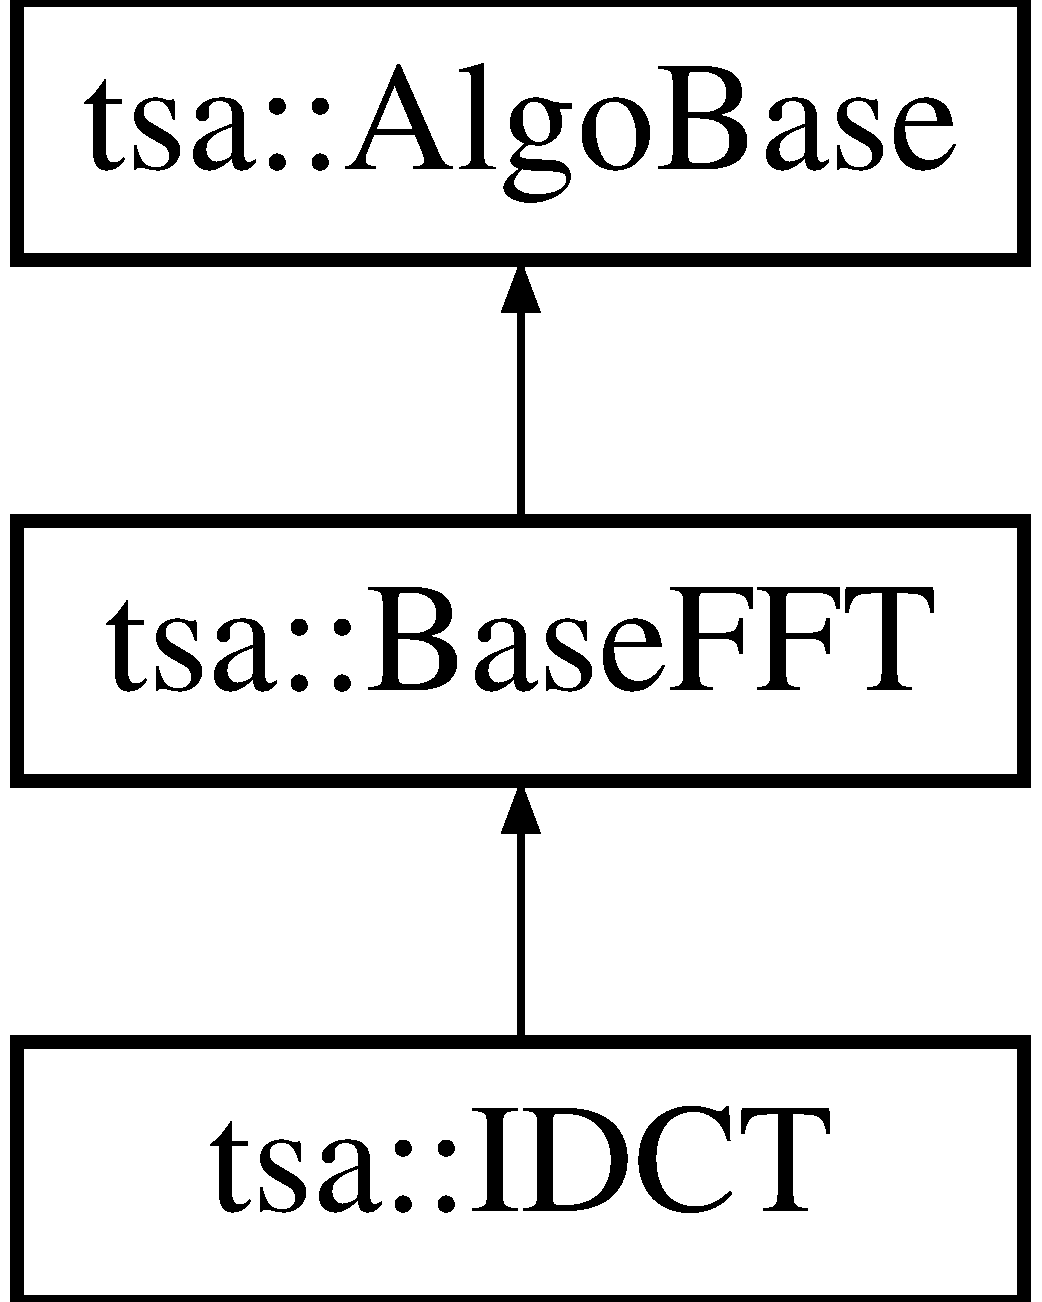
\includegraphics[height=3.000000cm]{classtsa_1_1_i_d_c_t}
\end{center}
\end{figure}
\subsection*{Public Member Functions}
\begin{DoxyCompactItemize}
\item 
\hyperlink{classtsa_1_1_i_d_c_t_abf50b114d212adc9d1c977db4eee9053}{I\+D\+CT} (int size=0, enum \hyperlink{namespacetsa_a217e07ef78939f88b22c8428ac96b1ae}{F\+F\+T\+Planning\+Mode} mode=\hyperlink{namespacetsa_a217e07ef78939f88b22c8428ac96b1aea2762be66fb6f3e4772c7f4cc162b9750}{E\+S\+T\+I\+M\+A\+TE}, bool Preserve\+Input=true)
\item 
\hyperlink{classtsa_1_1_i_d_c_t_a6747b5a2d41cdd4451e545ff129d5c13}{I\+D\+CT} (const \hyperlink{classtsa_1_1_i_d_c_t}{I\+D\+CT} \&from)
\item 
virtual \hyperlink{classtsa_1_1_i_d_c_t_ae7caa3512626cc407690fc0b9f7eaafb}{$\sim$\+I\+D\+CT} ()
\end{DoxyCompactItemize}
\begin{Indent}\textbf{ Operations}\par
\begin{DoxyCompactItemize}
\item 
void \hyperlink{classtsa_1_1_i_d_c_t_a9c1f5bc33388179e85f00882022cf567}{operator()} (\hyperlink{namespacetsa_ac599574bcc094eda25613724b8f3ca9e}{Seq\+View\+Double} \&in, \hyperlink{namespacetsa_ac599574bcc094eda25613724b8f3ca9e}{Seq\+View\+Double} \&out)
\item 
void \hyperlink{classtsa_1_1_i_d_c_t_aef29c6eb84ce3367e90eb66b3e40c005}{execute} (\hyperlink{namespacetsa_ad260cd21c1891c4ed391fe788569aba4}{Dmatrix} \&in, \hyperlink{namespacetsa_ad260cd21c1891c4ed391fe788569aba4}{Dmatrix} \&out)  throw (bad\+\_\+matrix\+\_\+size)
\item 
void \hyperlink{classtsa_1_1_i_d_c_t_a8bb130d39013848471a191f45e93fb09}{execute} (\hyperlink{namespacetsa_a8900fb03d849baf447a1a0efe2561fb2}{Dvector} \&in, \hyperlink{namespacetsa_a8900fb03d849baf447a1a0efe2561fb2}{Dvector} \&out)  throw (bad\+\_\+vector\+\_\+size)
\item 
void \hyperlink{classtsa_1_1_i_d_c_t_a3add06359e79507105820496b324ad7a}{Make\+Plan} ()  throw (std\+::runtime\+\_\+error)
\end{DoxyCompactItemize}
\end{Indent}
\subsection*{Additional Inherited Members}


\subsection{Detailed Description}
Multichannel Discrete Cosine Transform. 

Definition at line 73 of file I\+D\+C\+T.\+hpp.



\subsection{Constructor \& Destructor Documentation}
\mbox{\Hypertarget{classtsa_1_1_i_d_c_t_abf50b114d212adc9d1c977db4eee9053}\label{classtsa_1_1_i_d_c_t_abf50b114d212adc9d1c977db4eee9053}} 
\index{tsa\+::\+I\+D\+CT@{tsa\+::\+I\+D\+CT}!I\+D\+CT@{I\+D\+CT}}
\index{I\+D\+CT@{I\+D\+CT}!tsa\+::\+I\+D\+CT@{tsa\+::\+I\+D\+CT}}
\subsubsection{\texorpdfstring{I\+D\+C\+T()}{IDCT()}\hspace{0.1cm}{\footnotesize\ttfamily [1/2]}}
{\footnotesize\ttfamily tsa\+::\+I\+D\+C\+T\+::\+I\+D\+CT (\begin{DoxyParamCaption}\item[{int}]{size = {\ttfamily 0},  }\item[{enum \hyperlink{namespacetsa_a217e07ef78939f88b22c8428ac96b1ae}{F\+F\+T\+Planning\+Mode}}]{mode = {\ttfamily \hyperlink{namespacetsa_a217e07ef78939f88b22c8428ac96b1aea2762be66fb6f3e4772c7f4cc162b9750}{E\+S\+T\+I\+M\+A\+TE}},  }\item[{bool}]{Preserve\+Input = {\ttfamily true} }\end{DoxyParamCaption})}

Constructor


\begin{DoxyParams}{Parameters}
{\em size} & the size of the transform \\
\hline
{\em mode} & specify the way in which plans are calculated \\
\hline
{\em Preserve\+Input} & true if the input buffer must be preserved during the transform, false otherwise \\
\hline
\end{DoxyParams}


Definition at line 5 of file I\+D\+C\+T.\+cpp.

\mbox{\Hypertarget{classtsa_1_1_i_d_c_t_a6747b5a2d41cdd4451e545ff129d5c13}\label{classtsa_1_1_i_d_c_t_a6747b5a2d41cdd4451e545ff129d5c13}} 
\index{tsa\+::\+I\+D\+CT@{tsa\+::\+I\+D\+CT}!I\+D\+CT@{I\+D\+CT}}
\index{I\+D\+CT@{I\+D\+CT}!tsa\+::\+I\+D\+CT@{tsa\+::\+I\+D\+CT}}
\subsubsection{\texorpdfstring{I\+D\+C\+T()}{IDCT()}\hspace{0.1cm}{\footnotesize\ttfamily [2/2]}}
{\footnotesize\ttfamily tsa\+::\+I\+D\+C\+T\+::\+I\+D\+CT (\begin{DoxyParamCaption}\item[{const \hyperlink{classtsa_1_1_i_d_c_t}{I\+D\+CT} \&}]{from }\end{DoxyParamCaption})}

Copy constructor


\begin{DoxyParams}{Parameters}
{\em from} & The instance that must be copied \\
\hline
\end{DoxyParams}


Definition at line 11 of file I\+D\+C\+T.\+cpp.

\mbox{\Hypertarget{classtsa_1_1_i_d_c_t_ae7caa3512626cc407690fc0b9f7eaafb}\label{classtsa_1_1_i_d_c_t_ae7caa3512626cc407690fc0b9f7eaafb}} 
\index{tsa\+::\+I\+D\+CT@{tsa\+::\+I\+D\+CT}!````~I\+D\+CT@{$\sim$\+I\+D\+CT}}
\index{````~I\+D\+CT@{$\sim$\+I\+D\+CT}!tsa\+::\+I\+D\+CT@{tsa\+::\+I\+D\+CT}}
\subsubsection{\texorpdfstring{$\sim$\+I\+D\+C\+T()}{~IDCT()}}
{\footnotesize\ttfamily tsa\+::\+I\+D\+C\+T\+::$\sim$\+I\+D\+CT (\begin{DoxyParamCaption}{ }\end{DoxyParamCaption})\hspace{0.3cm}{\ttfamily [virtual]}}

Destructor 

Definition at line 17 of file I\+D\+C\+T.\+cpp.



\subsection{Member Function Documentation}
\mbox{\Hypertarget{classtsa_1_1_i_d_c_t_aef29c6eb84ce3367e90eb66b3e40c005}\label{classtsa_1_1_i_d_c_t_aef29c6eb84ce3367e90eb66b3e40c005}} 
\index{tsa\+::\+I\+D\+CT@{tsa\+::\+I\+D\+CT}!execute@{execute}}
\index{execute@{execute}!tsa\+::\+I\+D\+CT@{tsa\+::\+I\+D\+CT}}
\subsubsection{\texorpdfstring{execute()}{execute()}\hspace{0.1cm}{\footnotesize\ttfamily [1/2]}}
{\footnotesize\ttfamily void tsa\+::\+I\+D\+C\+T\+::execute (\begin{DoxyParamCaption}\item[{\hyperlink{namespacetsa_ad260cd21c1891c4ed391fe788569aba4}{Dmatrix} \&}]{in,  }\item[{\hyperlink{namespacetsa_ad260cd21c1891c4ed391fe788569aba4}{Dmatrix} \&}]{out }\end{DoxyParamCaption}) throw  \hyperlink{classtsa_1_1bad__matrix__size}{bad\+\_\+matrix\+\_\+size}) }

Execution of the fft of a multichannel buffer of double. Input data are organized in a matrix. Each row is a different channel, and the number of data to transform is equal to the number of columns. Both the number of rows and the number of columns can change between each call to this method. If the number of rows changes nothing special will happen, if the number of cols changes the plan is reevaluated with the current flags.

\begin{DoxyPrecond}{Precondition}
The number of rows of input and output matrix must be the same. 

The columns of the output matrix must be int(n/2)+1, where n is the number of columns of the input matrix.
\end{DoxyPrecond}
\begin{DoxyPostcond}{Postcondition}
the input buffer is unchanged, unless Set\+Preserve\+Input(false) was called 

the output buffer contain the fft of the input data
\end{DoxyPostcond}

\begin{DoxyExceptions}{Exceptions}
{\em \hyperlink{classtsa_1_1bad__matrix__size}{bad\+\_\+matrix\+\_\+size}} & the size of the output matrix is wrong \\
\hline
\end{DoxyExceptions}

\begin{DoxyParams}{Parameters}
{\em in} & reference to the input multichannel buffer \\
\hline
{\em out} & reference to the output multichannel buffer \\
\hline
\end{DoxyParams}


Definition at line 42 of file I\+D\+C\+T.\+cpp.

\mbox{\Hypertarget{classtsa_1_1_i_d_c_t_a8bb130d39013848471a191f45e93fb09}\label{classtsa_1_1_i_d_c_t_a8bb130d39013848471a191f45e93fb09}} 
\index{tsa\+::\+I\+D\+CT@{tsa\+::\+I\+D\+CT}!execute@{execute}}
\index{execute@{execute}!tsa\+::\+I\+D\+CT@{tsa\+::\+I\+D\+CT}}
\subsubsection{\texorpdfstring{execute()}{execute()}\hspace{0.1cm}{\footnotesize\ttfamily [2/2]}}
{\footnotesize\ttfamily void tsa\+::\+I\+D\+C\+T\+::execute (\begin{DoxyParamCaption}\item[{\hyperlink{namespacetsa_a8900fb03d849baf447a1a0efe2561fb2}{Dvector} \&}]{in,  }\item[{\hyperlink{namespacetsa_a8900fb03d849baf447a1a0efe2561fb2}{Dvector} \&}]{out }\end{DoxyParamCaption}) throw  \hyperlink{classtsa_1_1bad__vector__size}{bad\+\_\+vector\+\_\+size}) }

Execution of the fft of a single channel buffer of double. If the number of the buffer changes the plan is reevaluated with the current flags.

\begin{DoxyPrecond}{Precondition}
The sized of the output vector must be int(n/2)+1, where n is the size of the input vector.
\end{DoxyPrecond}
\begin{DoxyPostcond}{Postcondition}
the input buffer is unchanged, unless Set\+Preserve\+Input(false) was called 

the output buffer contain the fft of the input data
\end{DoxyPostcond}

\begin{DoxyExceptions}{Exceptions}
{\em \hyperlink{classtsa_1_1bad__matrix__size}{bad\+\_\+matrix\+\_\+size}} & the size of the output matrix is wrong \\
\hline
\end{DoxyExceptions}

\begin{DoxyParams}{Parameters}
{\em in} & reference to the input buffer \\
\hline
{\em out} & reference to the output buffer \\
\hline
\end{DoxyParams}


Definition at line 71 of file I\+D\+C\+T.\+cpp.

\mbox{\Hypertarget{classtsa_1_1_i_d_c_t_a3add06359e79507105820496b324ad7a}\label{classtsa_1_1_i_d_c_t_a3add06359e79507105820496b324ad7a}} 
\index{tsa\+::\+I\+D\+CT@{tsa\+::\+I\+D\+CT}!Make\+Plan@{Make\+Plan}}
\index{Make\+Plan@{Make\+Plan}!tsa\+::\+I\+D\+CT@{tsa\+::\+I\+D\+CT}}
\subsubsection{\texorpdfstring{Make\+Plan()}{MakePlan()}}
{\footnotesize\ttfamily void tsa\+::\+I\+D\+C\+T\+::\+Make\+Plan (\begin{DoxyParamCaption}{ }\end{DoxyParamCaption}) throw  std\+::runtime\+\_\+error) \hspace{0.3cm}{\ttfamily [virtual]}}

Make a new plan, with the current parameters.


\begin{DoxyExceptions}{Exceptions}
{\em std\+::runtime\+\_\+error} & The new plan cannot be created \\
\hline
\end{DoxyExceptions}


Implements \hyperlink{classtsa_1_1_base_f_f_t_a9af0c36413173821cac8dbdce9cfe3b4}{tsa\+::\+Base\+F\+FT}.



Definition at line 95 of file I\+D\+C\+T.\+cpp.

\mbox{\Hypertarget{classtsa_1_1_i_d_c_t_a9c1f5bc33388179e85f00882022cf567}\label{classtsa_1_1_i_d_c_t_a9c1f5bc33388179e85f00882022cf567}} 
\index{tsa\+::\+I\+D\+CT@{tsa\+::\+I\+D\+CT}!operator()@{operator()}}
\index{operator()@{operator()}!tsa\+::\+I\+D\+CT@{tsa\+::\+I\+D\+CT}}
\subsubsection{\texorpdfstring{operator()()}{operator()()}}
{\footnotesize\ttfamily void tsa\+::\+I\+D\+C\+T\+::operator() (\begin{DoxyParamCaption}\item[{\hyperlink{namespacetsa_ac599574bcc094eda25613724b8f3ca9e}{Seq\+View\+Double} \&}]{in,  }\item[{\hyperlink{namespacetsa_ac599574bcc094eda25613724b8f3ca9e}{Seq\+View\+Double} \&}]{out }\end{DoxyParamCaption})}

Apply the transformation on the data


\begin{DoxyParams}{Parameters}
{\em in} & a reference to the buffer containing the input data \\
\hline
{\em out} & a reference to the buffer containing the input data\\
\hline
\end{DoxyParams}
\begin{DoxyReturn}{Returns}
a reference to this instance of the class 
\end{DoxyReturn}


Definition at line 21 of file I\+D\+C\+T.\+cpp.



The documentation for this class was generated from the following files\+:\begin{DoxyCompactItemize}
\item 
/home/filip/\+Ph\+D/\+W\+D\+F\+Pipe\+\_\+test/p4\+T\+S\+A/include/\hyperlink{_i_d_c_t_8hpp}{I\+D\+C\+T.\+hpp}\item 
/home/filip/\+Ph\+D/\+W\+D\+F\+Pipe\+\_\+test/p4\+T\+S\+A/src/\hyperlink{_i_d_c_t_8cpp}{I\+D\+C\+T.\+cpp}\end{DoxyCompactItemize}

\hypertarget{classeternity_1_1_ifactory}{}\section{eternity\+:\+:Ifactory Class Reference}
\label{classeternity_1_1_ifactory}\index{eternity\+::\+Ifactory@{eternity\+::\+Ifactory}}


{\ttfamily \#include $<$dynamic.\+hpp$>$}

Inheritance diagram for eternity\+:\+:Ifactory\+:\begin{figure}[H]
\begin{center}
\leavevmode
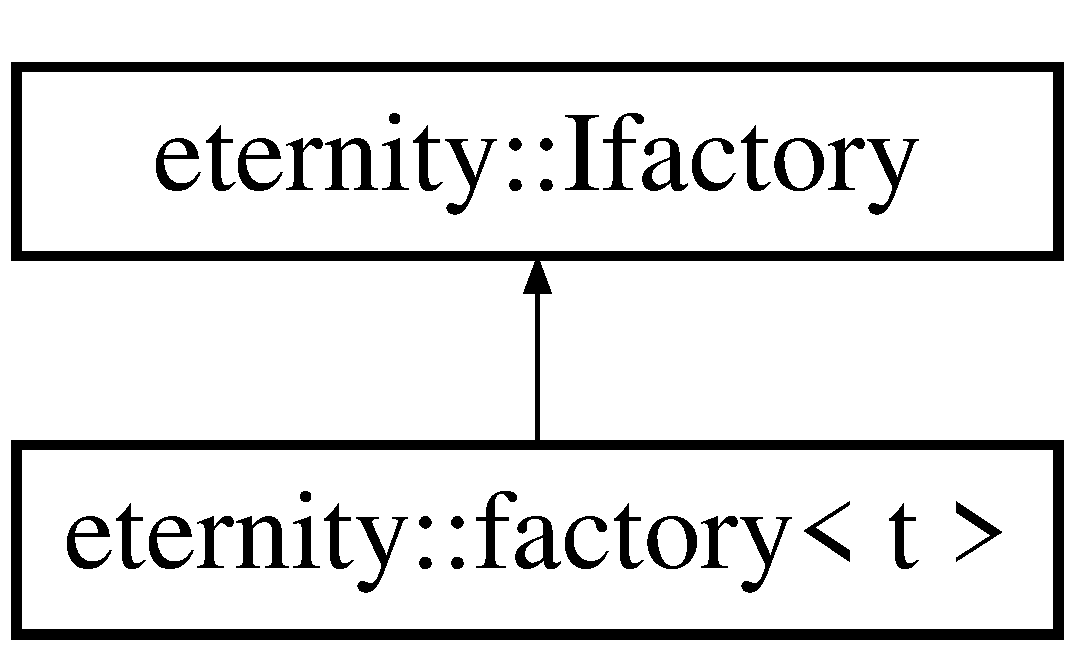
\includegraphics[height=2.000000cm]{classeternity_1_1_ifactory}
\end{center}
\end{figure}
\subsection*{Public Member Functions}
\begin{DoxyCompactItemize}
\item 
virtual \hyperlink{classeternity_1_1_ifactory_a5bcc4b3255bd1030562e0e554ece0a05}{$\sim$\+Ifactory} ()
\item 
virtual void $\ast$ \hyperlink{classeternity_1_1_ifactory_afaca5a9abf52fa3a731c3dfed7cb73b3}{create} (std\+::string \&class\+\_\+name)=0
\item 
virtual std\+::string \hyperlink{classeternity_1_1_ifactory_a6c2afa73d61aaa81233ab1216c508252}{get\+\_\+conventional\+\_\+name} (std\+::string \&compiler\+\_\+name)=0
\end{DoxyCompactItemize}
\subsection*{Public Attributes}
\begin{DoxyCompactItemize}
\item 
\hyperlink{classeternity_1_1_ifactory}{Ifactory} $\ast$ \hyperlink{classeternity_1_1_ifactory_a6749c6d3f8aea62a3084c0825f0687c5}{m\+\_\+p\+Next}
\begin{DoxyCompactList}\small\item\em The next item in global factory$<$t$>$ list. \end{DoxyCompactList}\end{DoxyCompactItemize}
\subsection*{Static Public Attributes}
\begin{DoxyCompactItemize}
\item 
static \hyperlink{classeternity_1_1_ifactory}{Ifactory} $\ast$ \hyperlink{classeternity_1_1_ifactory_a106788b385d5f378cb75bfb8f0296525}{m\+\_\+p\+Head} = 0
\begin{DoxyCompactList}\small\item\em The fist object in global factory$<$t$>$ list. \end{DoxyCompactList}\end{DoxyCompactItemize}


\subsection{Detailed Description}
\hyperlink{classeternity_1_1_ifactory}{Ifactory} is the base abstract class design to manage in the same way all template classes factory$<$t$>$. 

Definition at line 36 of file dynamic.\+hpp.



\subsection{Constructor \& Destructor Documentation}
\mbox{\Hypertarget{classeternity_1_1_ifactory_a5bcc4b3255bd1030562e0e554ece0a05}\label{classeternity_1_1_ifactory_a5bcc4b3255bd1030562e0e554ece0a05}} 
\index{eternity\+::\+Ifactory@{eternity\+::\+Ifactory}!````~Ifactory@{$\sim$\+Ifactory}}
\index{````~Ifactory@{$\sim$\+Ifactory}!eternity\+::\+Ifactory@{eternity\+::\+Ifactory}}
\subsubsection{\texorpdfstring{$\sim$\+Ifactory()}{~Ifactory()}}
{\footnotesize\ttfamily virtual eternity\+::\+Ifactory\+::$\sim$\+Ifactory (\begin{DoxyParamCaption}{ }\end{DoxyParamCaption})\hspace{0.3cm}{\ttfamily [inline]}, {\ttfamily [virtual]}}



Definition at line 39 of file dynamic.\+hpp.



\subsection{Member Function Documentation}
\mbox{\Hypertarget{classeternity_1_1_ifactory_afaca5a9abf52fa3a731c3dfed7cb73b3}\label{classeternity_1_1_ifactory_afaca5a9abf52fa3a731c3dfed7cb73b3}} 
\index{eternity\+::\+Ifactory@{eternity\+::\+Ifactory}!create@{create}}
\index{create@{create}!eternity\+::\+Ifactory@{eternity\+::\+Ifactory}}
\subsubsection{\texorpdfstring{create()}{create()}}
{\footnotesize\ttfamily virtual void$\ast$ eternity\+::\+Ifactory\+::create (\begin{DoxyParamCaption}\item[{std\+::string \&}]{class\+\_\+name }\end{DoxyParamCaption})\hspace{0.3cm}{\ttfamily [pure virtual]}}

The signature of create method for derived classes. 

Implemented in \hyperlink{classeternity_1_1factory_a08c1c494bc749955f9b0767d31933c2b}{eternity\+::factory$<$ t $>$}.

\mbox{\Hypertarget{classeternity_1_1_ifactory_a6c2afa73d61aaa81233ab1216c508252}\label{classeternity_1_1_ifactory_a6c2afa73d61aaa81233ab1216c508252}} 
\index{eternity\+::\+Ifactory@{eternity\+::\+Ifactory}!get\+\_\+conventional\+\_\+name@{get\+\_\+conventional\+\_\+name}}
\index{get\+\_\+conventional\+\_\+name@{get\+\_\+conventional\+\_\+name}!eternity\+::\+Ifactory@{eternity\+::\+Ifactory}}
\subsubsection{\texorpdfstring{get\+\_\+conventional\+\_\+name()}{get\_conventional\_name()}}
{\footnotesize\ttfamily virtual std\+::string eternity\+::\+Ifactory\+::get\+\_\+conventional\+\_\+name (\begin{DoxyParamCaption}\item[{std\+::string \&}]{compiler\+\_\+name }\end{DoxyParamCaption})\hspace{0.3cm}{\ttfamily [pure virtual]}}

The signature of get\+\_\+conventional\+\_\+name method for derived classes. 

Implemented in \hyperlink{classeternity_1_1factory_a0b7c7bc194b178379eb1b880f87d3b48}{eternity\+::factory$<$ t $>$}.



\subsection{Member Data Documentation}
\mbox{\Hypertarget{classeternity_1_1_ifactory_a106788b385d5f378cb75bfb8f0296525}\label{classeternity_1_1_ifactory_a106788b385d5f378cb75bfb8f0296525}} 
\index{eternity\+::\+Ifactory@{eternity\+::\+Ifactory}!m\+\_\+p\+Head@{m\+\_\+p\+Head}}
\index{m\+\_\+p\+Head@{m\+\_\+p\+Head}!eternity\+::\+Ifactory@{eternity\+::\+Ifactory}}
\subsubsection{\texorpdfstring{m\+\_\+p\+Head}{m\_pHead}}
{\footnotesize\ttfamily \hyperlink{classeternity_1_1_ifactory}{Ifactory} $\ast$ eternity\+::\+Ifactory\+::m\+\_\+p\+Head = 0\hspace{0.3cm}{\ttfamily [static]}}



The fist object in global factory$<$t$>$ list. 

All instancied factory$<$t$>$ are collect inside an unique global list. m\+\_\+p\+Head is the head of that list. 

Definition at line 40 of file dynamic.\+hpp.

\mbox{\Hypertarget{classeternity_1_1_ifactory_a6749c6d3f8aea62a3084c0825f0687c5}\label{classeternity_1_1_ifactory_a6749c6d3f8aea62a3084c0825f0687c5}} 
\index{eternity\+::\+Ifactory@{eternity\+::\+Ifactory}!m\+\_\+p\+Next@{m\+\_\+p\+Next}}
\index{m\+\_\+p\+Next@{m\+\_\+p\+Next}!eternity\+::\+Ifactory@{eternity\+::\+Ifactory}}
\subsubsection{\texorpdfstring{m\+\_\+p\+Next}{m\_pNext}}
{\footnotesize\ttfamily \hyperlink{classeternity_1_1_ifactory}{Ifactory}$\ast$ eternity\+::\+Ifactory\+::m\+\_\+p\+Next}



The next item in global factory$<$t$>$ list. 

Each item in the gloabl list of factory$<$t$>$ object has a pointer to the next item named m\+\_\+p\+Next. The last element has a N\+U\+LL value inside m\+\_\+p\+Next. 

Definition at line 55 of file dynamic.\+hpp.



The documentation for this class was generated from the following files\+:\begin{DoxyCompactItemize}
\item 
/home/filip/\+Ph\+D/\+W\+D\+F\+Pipe\+\_\+test/p4\+T\+S\+A/include/eternity/\hyperlink{dynamic_8hpp}{dynamic.\+hpp}\item 
/home/filip/\+Ph\+D/\+W\+D\+F\+Pipe\+\_\+test/p4\+T\+S\+A/include/eternity/\hyperlink{dynamic_8cpp}{dynamic.\+cpp}\end{DoxyCompactItemize}

\hypertarget{classtsa_1_1_inverse_real_f_f_t}{}\section{tsa\+:\+:Inverse\+Real\+F\+FT Class Reference}
\label{classtsa_1_1_inverse_real_f_f_t}\index{tsa\+::\+Inverse\+Real\+F\+FT@{tsa\+::\+Inverse\+Real\+F\+FT}}


Multichannel inverse real to complex F\+FT.  




{\ttfamily \#include $<$Inverse\+Real\+F\+F\+T.\+hpp$>$}

Inheritance diagram for tsa\+:\+:Inverse\+Real\+F\+FT\+:\begin{figure}[H]
\begin{center}
\leavevmode
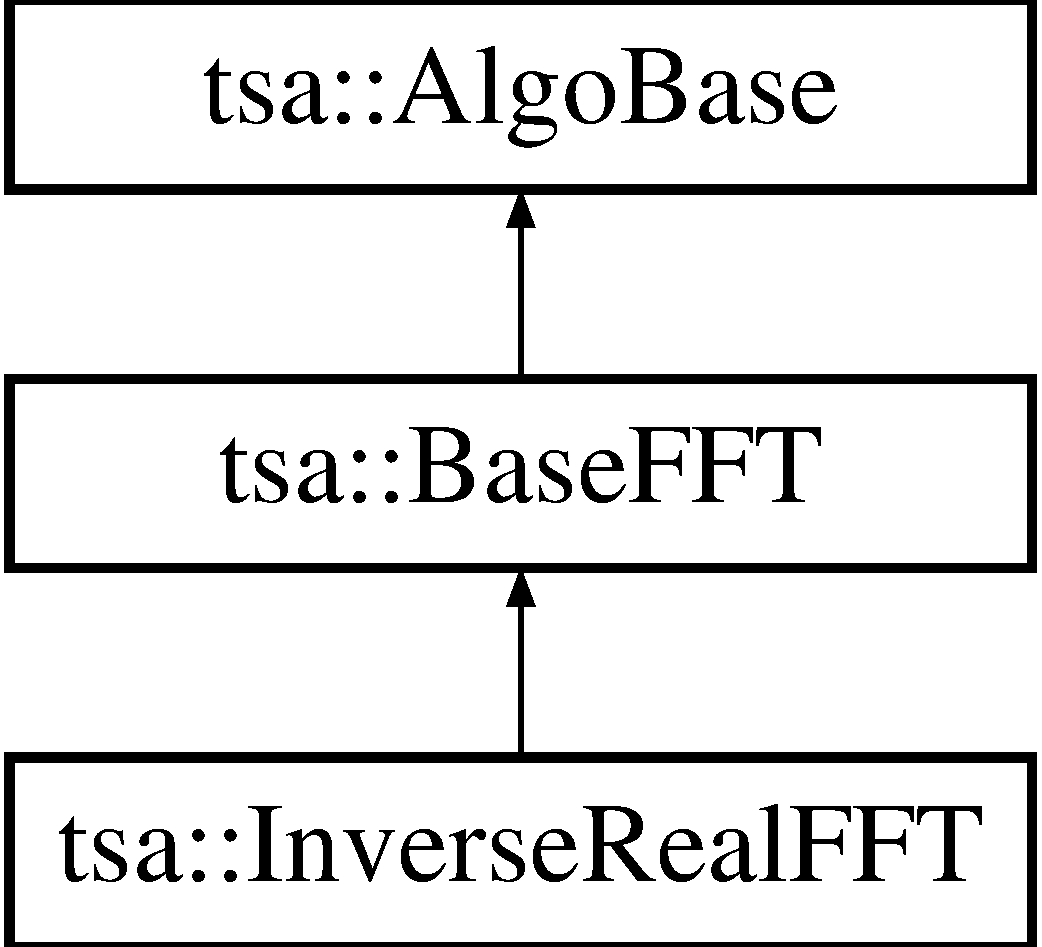
\includegraphics[height=3.000000cm]{classtsa_1_1_inverse_real_f_f_t}
\end{center}
\end{figure}
\subsection*{Public Member Functions}
\begin{DoxyCompactItemize}
\item 
\hyperlink{classtsa_1_1_inverse_real_f_f_t_a50258b4d4596d93935791135cd22feb9}{Inverse\+Real\+F\+FT} (int size=0, enum \hyperlink{namespacetsa_a217e07ef78939f88b22c8428ac96b1ae}{F\+F\+T\+Planning\+Mode} mode=\hyperlink{namespacetsa_a217e07ef78939f88b22c8428ac96b1aea2762be66fb6f3e4772c7f4cc162b9750}{E\+S\+T\+I\+M\+A\+TE}, bool Preserve\+Input=false)
\item 
\hyperlink{classtsa_1_1_inverse_real_f_f_t_a5a9e17eaf4fd69e719dca4b881010876}{Inverse\+Real\+F\+FT} (const \hyperlink{classtsa_1_1_inverse_real_f_f_t}{Inverse\+Real\+F\+FT} \&from)
\item 
\hyperlink{classtsa_1_1_inverse_real_f_f_t_a928e08fb19e46a901e0dc42ec5970801}{$\sim$\+Inverse\+Real\+F\+FT} ()
\end{DoxyCompactItemize}
\begin{Indent}\textbf{ Operations}\par
\begin{DoxyCompactItemize}
\item 
void \hyperlink{classtsa_1_1_inverse_real_f_f_t_a619333f55b1526e03169c9c8be29d442}{operator()} (\hyperlink{namespacetsa_ab32775c889b53c40fa83939f22372b75}{Seq\+View\+Complex} \&in, \hyperlink{namespacetsa_ac599574bcc094eda25613724b8f3ca9e}{Seq\+View\+Double} \&out)
\item 
void \hyperlink{classtsa_1_1_inverse_real_f_f_t_ac37c11d801f396360818a54dddf1c9d1}{execute} (\hyperlink{namespacetsa_a86348fef1603a135fe5fba9e5f5486ee}{Cmatrix} \&in, \hyperlink{namespacetsa_ad260cd21c1891c4ed391fe788569aba4}{Dmatrix} \&out)  throw (bad\+\_\+matrix\+\_\+size)
\item 
void \hyperlink{classtsa_1_1_inverse_real_f_f_t_a2693642ff2282921710456dea0915b40}{execute} (\hyperlink{namespacetsa_a054d1045ead95a65819e9e5722baf600}{Cvector} \&in, \hyperlink{namespacetsa_a8900fb03d849baf447a1a0efe2561fb2}{Dvector} \&out)  throw (bad\+\_\+vector\+\_\+size)
\item 
void \hyperlink{classtsa_1_1_inverse_real_f_f_t_aaa4b1dd80a308eb09a9dc9fe1aeba51e}{execute} (\hyperlink{namespacetsa_ad294f56c16152a1618cbe2f19b768e2e}{Cmatrix\+Row} \&in, \hyperlink{namespacetsa_aeaf3be962a114beef3d9e89b0fb49bf4}{Dmatrix\+Row} \&out)  throw (bad\+\_\+vector\+\_\+size)
\item 
void \hyperlink{classtsa_1_1_inverse_real_f_f_t_a6264c0d0b0b4a31e584a390b06281631}{execute} (\hyperlink{namespacetsa_ad294f56c16152a1618cbe2f19b768e2e}{Cmatrix\+Row} \&in, \hyperlink{namespacetsa_aeaf3be962a114beef3d9e89b0fb49bf4}{Dmatrix\+Row} \&out, unsigned int insize)  throw (bad\+\_\+vector\+\_\+size)
\item 
void \hyperlink{classtsa_1_1_inverse_real_f_f_t_ae5b45701f989efce89c6c336ec78c189}{Make\+Plan} ()  throw (std\+::runtime\+\_\+error)
\end{DoxyCompactItemize}
\end{Indent}
\subsection*{Additional Inherited Members}


\subsection{Detailed Description}
Multichannel inverse real to complex F\+FT. 

This is the implementation of the F\+FT of a real multichannel buffer 

Definition at line 66 of file Inverse\+Real\+F\+F\+T.\+hpp.



\subsection{Constructor \& Destructor Documentation}
\mbox{\Hypertarget{classtsa_1_1_inverse_real_f_f_t_a50258b4d4596d93935791135cd22feb9}\label{classtsa_1_1_inverse_real_f_f_t_a50258b4d4596d93935791135cd22feb9}} 
\index{tsa\+::\+Inverse\+Real\+F\+FT@{tsa\+::\+Inverse\+Real\+F\+FT}!Inverse\+Real\+F\+FT@{Inverse\+Real\+F\+FT}}
\index{Inverse\+Real\+F\+FT@{Inverse\+Real\+F\+FT}!tsa\+::\+Inverse\+Real\+F\+FT@{tsa\+::\+Inverse\+Real\+F\+FT}}
\subsubsection{\texorpdfstring{Inverse\+Real\+F\+F\+T()}{InverseRealFFT()}\hspace{0.1cm}{\footnotesize\ttfamily [1/2]}}
{\footnotesize\ttfamily tsa\+::\+Inverse\+Real\+F\+F\+T\+::\+Inverse\+Real\+F\+FT (\begin{DoxyParamCaption}\item[{int}]{size = {\ttfamily 0},  }\item[{enum \hyperlink{namespacetsa_a217e07ef78939f88b22c8428ac96b1ae}{F\+F\+T\+Planning\+Mode}}]{mode = {\ttfamily \hyperlink{namespacetsa_a217e07ef78939f88b22c8428ac96b1aea2762be66fb6f3e4772c7f4cc162b9750}{E\+S\+T\+I\+M\+A\+TE}},  }\item[{bool}]{Preserve\+Input = {\ttfamily false} }\end{DoxyParamCaption})}

Constructor


\begin{DoxyParams}{Parameters}
{\em size} & the size of the transform \\
\hline
{\em mode} & specify the way in which plans are calculated \\
\hline
{\em Preserve\+Input} & true if the input buffer must be preserved during the transform, false otherwise \\
\hline
\end{DoxyParams}


Definition at line 5 of file Inverse\+Real\+F\+F\+T.\+cpp.

\mbox{\Hypertarget{classtsa_1_1_inverse_real_f_f_t_a5a9e17eaf4fd69e719dca4b881010876}\label{classtsa_1_1_inverse_real_f_f_t_a5a9e17eaf4fd69e719dca4b881010876}} 
\index{tsa\+::\+Inverse\+Real\+F\+FT@{tsa\+::\+Inverse\+Real\+F\+FT}!Inverse\+Real\+F\+FT@{Inverse\+Real\+F\+FT}}
\index{Inverse\+Real\+F\+FT@{Inverse\+Real\+F\+FT}!tsa\+::\+Inverse\+Real\+F\+FT@{tsa\+::\+Inverse\+Real\+F\+FT}}
\subsubsection{\texorpdfstring{Inverse\+Real\+F\+F\+T()}{InverseRealFFT()}\hspace{0.1cm}{\footnotesize\ttfamily [2/2]}}
{\footnotesize\ttfamily tsa\+::\+Inverse\+Real\+F\+F\+T\+::\+Inverse\+Real\+F\+FT (\begin{DoxyParamCaption}\item[{const \hyperlink{classtsa_1_1_inverse_real_f_f_t}{Inverse\+Real\+F\+FT} \&}]{from }\end{DoxyParamCaption})}

Copy constructor


\begin{DoxyParams}{Parameters}
{\em from} & The instance that must be copied \\
\hline
\end{DoxyParams}


Definition at line 11 of file Inverse\+Real\+F\+F\+T.\+cpp.

\mbox{\Hypertarget{classtsa_1_1_inverse_real_f_f_t_a928e08fb19e46a901e0dc42ec5970801}\label{classtsa_1_1_inverse_real_f_f_t_a928e08fb19e46a901e0dc42ec5970801}} 
\index{tsa\+::\+Inverse\+Real\+F\+FT@{tsa\+::\+Inverse\+Real\+F\+FT}!````~Inverse\+Real\+F\+FT@{$\sim$\+Inverse\+Real\+F\+FT}}
\index{````~Inverse\+Real\+F\+FT@{$\sim$\+Inverse\+Real\+F\+FT}!tsa\+::\+Inverse\+Real\+F\+FT@{tsa\+::\+Inverse\+Real\+F\+FT}}
\subsubsection{\texorpdfstring{$\sim$\+Inverse\+Real\+F\+F\+T()}{~InverseRealFFT()}}
{\footnotesize\ttfamily tsa\+::\+Inverse\+Real\+F\+F\+T\+::$\sim$\+Inverse\+Real\+F\+FT (\begin{DoxyParamCaption}{ }\end{DoxyParamCaption})}

Destructor 

Definition at line 17 of file Inverse\+Real\+F\+F\+T.\+cpp.



\subsection{Member Function Documentation}
\mbox{\Hypertarget{classtsa_1_1_inverse_real_f_f_t_ac37c11d801f396360818a54dddf1c9d1}\label{classtsa_1_1_inverse_real_f_f_t_ac37c11d801f396360818a54dddf1c9d1}} 
\index{tsa\+::\+Inverse\+Real\+F\+FT@{tsa\+::\+Inverse\+Real\+F\+FT}!execute@{execute}}
\index{execute@{execute}!tsa\+::\+Inverse\+Real\+F\+FT@{tsa\+::\+Inverse\+Real\+F\+FT}}
\subsubsection{\texorpdfstring{execute()}{execute()}\hspace{0.1cm}{\footnotesize\ttfamily [1/4]}}
{\footnotesize\ttfamily void tsa\+::\+Inverse\+Real\+F\+F\+T\+::execute (\begin{DoxyParamCaption}\item[{\hyperlink{namespacetsa_a86348fef1603a135fe5fba9e5f5486ee}{Cmatrix} \&}]{in,  }\item[{\hyperlink{namespacetsa_ad260cd21c1891c4ed391fe788569aba4}{Dmatrix} \&}]{out }\end{DoxyParamCaption}) throw  \hyperlink{classtsa_1_1bad__matrix__size}{bad\+\_\+matrix\+\_\+size}) }

Execution of the inverse real fft of a multichannel buffer of complex. Input data are organized in a matrix. Each row is a different channel, and the number of data to transform is equal to the number of columns. Both the number of rows and the number of columns can change between each call to this method. If the number of rows changes nothing special will happen, if the number of cols changes the plan is reevaluated with the current flags.

\begin{DoxyPrecond}{Precondition}
The number of rows of input and output matrix must be the same. 

The number of columns of the input matrix must be int(n/2)+1, where n is the number of columns of the output matrix.
\end{DoxyPrecond}
\begin{DoxyPostcond}{Postcondition}
the input buffer is changed, unless \hyperlink{classtsa_1_1_base_f_f_t_a5b1e2f36dbdfe197aa6c74d1cf963f40}{Set\+Preserve\+Input} was called with true argument 

the output buffer contain the inverse fft of the input data 
\end{DoxyPostcond}

\begin{DoxyExceptions}{Exceptions}
{\em \hyperlink{classtsa_1_1bad__matrix__size}{bad\+\_\+matrix\+\_\+size}} & the size of the output matrix is wrong\\
\hline
\end{DoxyExceptions}

\begin{DoxyParams}{Parameters}
{\em in} & reference to the input multichannel buffer \\
\hline
{\em out} & reference to the output multichannel buffer \\
\hline
\end{DoxyParams}


Definition at line 21 of file Inverse\+Real\+F\+F\+T.\+cpp.

\mbox{\Hypertarget{classtsa_1_1_inverse_real_f_f_t_a2693642ff2282921710456dea0915b40}\label{classtsa_1_1_inverse_real_f_f_t_a2693642ff2282921710456dea0915b40}} 
\index{tsa\+::\+Inverse\+Real\+F\+FT@{tsa\+::\+Inverse\+Real\+F\+FT}!execute@{execute}}
\index{execute@{execute}!tsa\+::\+Inverse\+Real\+F\+FT@{tsa\+::\+Inverse\+Real\+F\+FT}}
\subsubsection{\texorpdfstring{execute()}{execute()}\hspace{0.1cm}{\footnotesize\ttfamily [2/4]}}
{\footnotesize\ttfamily void tsa\+::\+Inverse\+Real\+F\+F\+T\+::execute (\begin{DoxyParamCaption}\item[{\hyperlink{namespacetsa_a054d1045ead95a65819e9e5722baf600}{Cvector} \&}]{in,  }\item[{\hyperlink{namespacetsa_a8900fb03d849baf447a1a0efe2561fb2}{Dvector} \&}]{out }\end{DoxyParamCaption}) throw  \hyperlink{classtsa_1_1bad__vector__size}{bad\+\_\+vector\+\_\+size}) }

Execution of the inverse real fft of a buffer of complex. If the number of data changes the plan is reevaluated with the current flags.

\begin{DoxyPrecond}{Precondition}
The number of columns of the input matrix must be int(n/2)+1, where n is the number of columns of the output matrix.
\end{DoxyPrecond}
\begin{DoxyPostcond}{Postcondition}
the input buffer is changed, unless \hyperlink{classtsa_1_1_base_f_f_t_a5b1e2f36dbdfe197aa6c74d1cf963f40}{Set\+Preserve\+Input} was called with true argument 

the output buffer contain the inverse fft of the input data 
\end{DoxyPostcond}

\begin{DoxyExceptions}{Exceptions}
{\em \hyperlink{classtsa_1_1bad__vector__size}{bad\+\_\+vector\+\_\+size}} & the size of the output vector\\
\hline
\end{DoxyExceptions}

\begin{DoxyParams}{Parameters}
{\em in} & reference to the input vector \\
\hline
{\em out} & reference to the output vector \\
\hline
\end{DoxyParams}


Definition at line 69 of file Inverse\+Real\+F\+F\+T.\+cpp.

\mbox{\Hypertarget{classtsa_1_1_inverse_real_f_f_t_aaa4b1dd80a308eb09a9dc9fe1aeba51e}\label{classtsa_1_1_inverse_real_f_f_t_aaa4b1dd80a308eb09a9dc9fe1aeba51e}} 
\index{tsa\+::\+Inverse\+Real\+F\+FT@{tsa\+::\+Inverse\+Real\+F\+FT}!execute@{execute}}
\index{execute@{execute}!tsa\+::\+Inverse\+Real\+F\+FT@{tsa\+::\+Inverse\+Real\+F\+FT}}
\subsubsection{\texorpdfstring{execute()}{execute()}\hspace{0.1cm}{\footnotesize\ttfamily [3/4]}}
{\footnotesize\ttfamily void tsa\+::\+Inverse\+Real\+F\+F\+T\+::execute (\begin{DoxyParamCaption}\item[{\hyperlink{namespacetsa_ad294f56c16152a1618cbe2f19b768e2e}{Cmatrix\+Row} \&}]{in,  }\item[{\hyperlink{namespacetsa_aeaf3be962a114beef3d9e89b0fb49bf4}{Dmatrix\+Row} \&}]{out }\end{DoxyParamCaption}) throw  \hyperlink{classtsa_1_1bad__vector__size}{bad\+\_\+vector\+\_\+size}) }



Definition at line 88 of file Inverse\+Real\+F\+F\+T.\+cpp.

\mbox{\Hypertarget{classtsa_1_1_inverse_real_f_f_t_a6264c0d0b0b4a31e584a390b06281631}\label{classtsa_1_1_inverse_real_f_f_t_a6264c0d0b0b4a31e584a390b06281631}} 
\index{tsa\+::\+Inverse\+Real\+F\+FT@{tsa\+::\+Inverse\+Real\+F\+FT}!execute@{execute}}
\index{execute@{execute}!tsa\+::\+Inverse\+Real\+F\+FT@{tsa\+::\+Inverse\+Real\+F\+FT}}
\subsubsection{\texorpdfstring{execute()}{execute()}\hspace{0.1cm}{\footnotesize\ttfamily [4/4]}}
{\footnotesize\ttfamily void tsa\+::\+Inverse\+Real\+F\+F\+T\+::execute (\begin{DoxyParamCaption}\item[{\hyperlink{namespacetsa_ad294f56c16152a1618cbe2f19b768e2e}{Cmatrix\+Row} \&}]{in,  }\item[{\hyperlink{namespacetsa_aeaf3be962a114beef3d9e89b0fb49bf4}{Dmatrix\+Row} \&}]{out,  }\item[{unsigned int}]{insize }\end{DoxyParamCaption}) throw  \hyperlink{classtsa_1_1bad__vector__size}{bad\+\_\+vector\+\_\+size}) }



Definition at line 107 of file Inverse\+Real\+F\+F\+T.\+cpp.

\mbox{\Hypertarget{classtsa_1_1_inverse_real_f_f_t_ae5b45701f989efce89c6c336ec78c189}\label{classtsa_1_1_inverse_real_f_f_t_ae5b45701f989efce89c6c336ec78c189}} 
\index{tsa\+::\+Inverse\+Real\+F\+FT@{tsa\+::\+Inverse\+Real\+F\+FT}!Make\+Plan@{Make\+Plan}}
\index{Make\+Plan@{Make\+Plan}!tsa\+::\+Inverse\+Real\+F\+FT@{tsa\+::\+Inverse\+Real\+F\+FT}}
\subsubsection{\texorpdfstring{Make\+Plan()}{MakePlan()}}
{\footnotesize\ttfamily void tsa\+::\+Inverse\+Real\+F\+F\+T\+::\+Make\+Plan (\begin{DoxyParamCaption}{ }\end{DoxyParamCaption}) throw  std\+::runtime\+\_\+error) \hspace{0.3cm}{\ttfamily [virtual]}}

Make a new plan, with the current parameters.


\begin{DoxyExceptions}{Exceptions}
{\em std\+::runtime\+\_\+error} & The new plan cannot be created \\
\hline
\end{DoxyExceptions}


Implements \hyperlink{classtsa_1_1_base_f_f_t_a9af0c36413173821cac8dbdce9cfe3b4}{tsa\+::\+Base\+F\+FT}.



Definition at line 130 of file Inverse\+Real\+F\+F\+T.\+cpp.

\mbox{\Hypertarget{classtsa_1_1_inverse_real_f_f_t_a619333f55b1526e03169c9c8be29d442}\label{classtsa_1_1_inverse_real_f_f_t_a619333f55b1526e03169c9c8be29d442}} 
\index{tsa\+::\+Inverse\+Real\+F\+FT@{tsa\+::\+Inverse\+Real\+F\+FT}!operator()@{operator()}}
\index{operator()@{operator()}!tsa\+::\+Inverse\+Real\+F\+FT@{tsa\+::\+Inverse\+Real\+F\+FT}}
\subsubsection{\texorpdfstring{operator()()}{operator()()}}
{\footnotesize\ttfamily void tsa\+::\+Inverse\+Real\+F\+F\+T\+::operator() (\begin{DoxyParamCaption}\item[{\hyperlink{namespacetsa_ab32775c889b53c40fa83939f22372b75}{Seq\+View\+Complex} \&}]{in,  }\item[{\hyperlink{namespacetsa_ac599574bcc094eda25613724b8f3ca9e}{Seq\+View\+Double} \&}]{out }\end{DoxyParamCaption})}

Apply the transformation on the data


\begin{DoxyParams}{Parameters}
{\em in} & a reference to the buffer containing the input data \\
\hline
{\em out} & a reference to the buffer containing the input data\\
\hline
\end{DoxyParams}
\begin{DoxyReturn}{Returns}
a reference to this instance of the class 
\end{DoxyReturn}


Definition at line 47 of file Inverse\+Real\+F\+F\+T.\+cpp.



The documentation for this class was generated from the following files\+:\begin{DoxyCompactItemize}
\item 
/home/filip/\+Ph\+D/\+W\+D\+F\+Pipe\+\_\+test/p4\+T\+S\+A/include/\hyperlink{_inverse_real_f_f_t_8hpp}{Inverse\+Real\+F\+F\+T.\+hpp}\item 
/home/filip/\+Ph\+D/\+W\+D\+F\+Pipe\+\_\+test/p4\+T\+S\+A/src/\hyperlink{_inverse_real_f_f_t_8cpp}{Inverse\+Real\+F\+F\+T.\+cpp}\end{DoxyCompactItemize}

\hypertarget{classtsa_1_1_kaiser_window}{}\section{tsa\+:\+:Kaiser\+Window Class Reference}
\label{classtsa_1_1_kaiser_window}\index{tsa\+::\+Kaiser\+Window@{tsa\+::\+Kaiser\+Window}}


Kaiser windowing algorithm Harris, F. J. \char`\"{}\+On the Use of Windows for Harmonic Analysis with the Discrete Fourier Transform.\char`\"{} Proceedings of the I\+E\+EE. Vol. 66 (January 1978). pp. 66-\/67.  




{\ttfamily \#include $<$Kaiser\+Window.\+hpp$>$}

Inheritance diagram for tsa\+:\+:Kaiser\+Window\+:\begin{figure}[H]
\begin{center}
\leavevmode
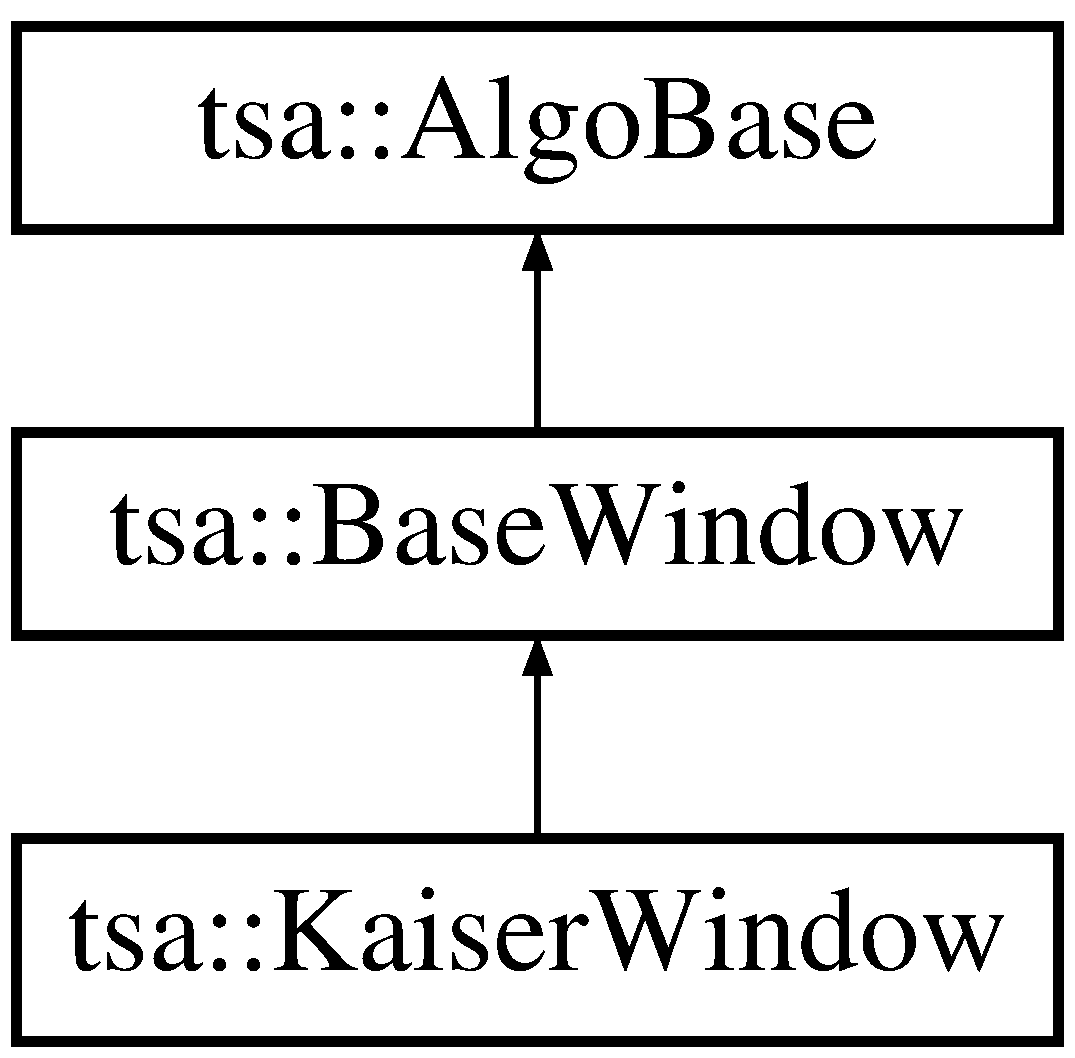
\includegraphics[height=3.000000cm]{classtsa_1_1_kaiser_window}
\end{center}
\end{figure}
\subsection*{Public Member Functions}
\begin{DoxyCompactItemize}
\item 
\hyperlink{classtsa_1_1_kaiser_window_a1435f80a21b198c05d60be076fa152b1}{Kaiser\+Window} (int size)
\item 
\hyperlink{classtsa_1_1_kaiser_window_ae1de2ef14d0c6b80161d0456502b4753}{Kaiser\+Window} (int size, const std\+::string \&par)
\item 
virtual \hyperlink{classtsa_1_1_kaiser_window_a98965a07384b404238a53bf9d66e8c77}{$\sim$\+Kaiser\+Window} ()
\end{DoxyCompactItemize}
\begin{Indent}\textbf{ Operations}\par
\begin{DoxyCompactItemize}
\item 
void \hyperlink{classtsa_1_1_kaiser_window_a02d18a272d16d54fa4f7c9e8b227356e}{operator()} (\hyperlink{namespacetsa_ac599574bcc094eda25613724b8f3ca9e}{Seq\+View\+Double} \&v1)
\item 
void \hyperlink{classtsa_1_1_kaiser_window_a94b99f1c961eadad783e44ccce9629e7}{operator()} (\hyperlink{namespacetsa_ac599574bcc094eda25613724b8f3ca9e}{Seq\+View\+Double} \&v1, \hyperlink{namespacetsa_ac599574bcc094eda25613724b8f3ca9e}{Seq\+View\+Double} \&v2)
\item 
void \hyperlink{classtsa_1_1_kaiser_window_ae573c5ab979c3292d10feddc5180b6b4}{Resize} (unsigned int size)
\end{DoxyCompactItemize}
\end{Indent}
\begin{Indent}\textbf{ Getters}\par
\begin{DoxyCompactItemize}
\item 
double \hyperlink{classtsa_1_1_kaiser_window_a12dbee6e0639e3f8b7bc1191c46d9798}{operator()} (int i)
\end{DoxyCompactItemize}
\end{Indent}
\subsection*{Private Member Functions}
\begin{DoxyCompactItemize}
\item 
void \hyperlink{classtsa_1_1_kaiser_window_a4799ed39290a058eea9d44df73f764ea}{Fill\+Window} ()
\end{DoxyCompactItemize}
\subsection*{Private Attributes}
\begin{DoxyCompactItemize}
\item 
double \hyperlink{classtsa_1_1_kaiser_window_a92c5708ea950eaf9845b13f2272cf43f}{m\+Alpha}
\end{DoxyCompactItemize}
\subsection*{Additional Inherited Members}


\subsection{Detailed Description}
Kaiser windowing algorithm Harris, F. J. \char`\"{}\+On the Use of Windows for Harmonic Analysis with the Discrete Fourier Transform.\char`\"{} Proceedings of the I\+E\+EE. Vol. 66 (January 1978). pp. 66-\/67. 

Definition at line 77 of file Kaiser\+Window.\+hpp.



\subsection{Constructor \& Destructor Documentation}
\mbox{\Hypertarget{classtsa_1_1_kaiser_window_a1435f80a21b198c05d60be076fa152b1}\label{classtsa_1_1_kaiser_window_a1435f80a21b198c05d60be076fa152b1}} 
\index{tsa\+::\+Kaiser\+Window@{tsa\+::\+Kaiser\+Window}!Kaiser\+Window@{Kaiser\+Window}}
\index{Kaiser\+Window@{Kaiser\+Window}!tsa\+::\+Kaiser\+Window@{tsa\+::\+Kaiser\+Window}}
\subsubsection{\texorpdfstring{Kaiser\+Window()}{KaiserWindow()}\hspace{0.1cm}{\footnotesize\ttfamily [1/2]}}
{\footnotesize\ttfamily tsa\+::\+Kaiser\+Window\+::\+Kaiser\+Window (\begin{DoxyParamCaption}\item[{int}]{size }\end{DoxyParamCaption})\hspace{0.3cm}{\ttfamily [inline]}}

Constructor


\begin{DoxyParams}{Parameters}
{\em size} & the size of the window \\
\hline
{\em cached} & true if the window must be preevaluated in a buffer \\
\hline
\end{DoxyParams}


Definition at line 86 of file Kaiser\+Window.\+hpp.

\mbox{\Hypertarget{classtsa_1_1_kaiser_window_ae1de2ef14d0c6b80161d0456502b4753}\label{classtsa_1_1_kaiser_window_ae1de2ef14d0c6b80161d0456502b4753}} 
\index{tsa\+::\+Kaiser\+Window@{tsa\+::\+Kaiser\+Window}!Kaiser\+Window@{Kaiser\+Window}}
\index{Kaiser\+Window@{Kaiser\+Window}!tsa\+::\+Kaiser\+Window@{tsa\+::\+Kaiser\+Window}}
\subsubsection{\texorpdfstring{Kaiser\+Window()}{KaiserWindow()}\hspace{0.1cm}{\footnotesize\ttfamily [2/2]}}
{\footnotesize\ttfamily tsa\+::\+Kaiser\+Window\+::\+Kaiser\+Window (\begin{DoxyParamCaption}\item[{int}]{size,  }\item[{const std\+::string \&}]{par }\end{DoxyParamCaption})\hspace{0.3cm}{\ttfamily [inline]}}



Definition at line 93 of file Kaiser\+Window.\+hpp.

\mbox{\Hypertarget{classtsa_1_1_kaiser_window_a98965a07384b404238a53bf9d66e8c77}\label{classtsa_1_1_kaiser_window_a98965a07384b404238a53bf9d66e8c77}} 
\index{tsa\+::\+Kaiser\+Window@{tsa\+::\+Kaiser\+Window}!````~Kaiser\+Window@{$\sim$\+Kaiser\+Window}}
\index{````~Kaiser\+Window@{$\sim$\+Kaiser\+Window}!tsa\+::\+Kaiser\+Window@{tsa\+::\+Kaiser\+Window}}
\subsubsection{\texorpdfstring{$\sim$\+Kaiser\+Window()}{~KaiserWindow()}}
{\footnotesize\ttfamily virtual tsa\+::\+Kaiser\+Window\+::$\sim$\+Kaiser\+Window (\begin{DoxyParamCaption}{ }\end{DoxyParamCaption})\hspace{0.3cm}{\ttfamily [inline]}, {\ttfamily [virtual]}}

Destructor 

Definition at line 104 of file Kaiser\+Window.\+hpp.



\subsection{Member Function Documentation}
\mbox{\Hypertarget{classtsa_1_1_kaiser_window_a4799ed39290a058eea9d44df73f764ea}\label{classtsa_1_1_kaiser_window_a4799ed39290a058eea9d44df73f764ea}} 
\index{tsa\+::\+Kaiser\+Window@{tsa\+::\+Kaiser\+Window}!Fill\+Window@{Fill\+Window}}
\index{Fill\+Window@{Fill\+Window}!tsa\+::\+Kaiser\+Window@{tsa\+::\+Kaiser\+Window}}
\subsubsection{\texorpdfstring{Fill\+Window()}{FillWindow()}}
{\footnotesize\ttfamily void tsa\+::\+Kaiser\+Window\+::\+Fill\+Window (\begin{DoxyParamCaption}{ }\end{DoxyParamCaption})\hspace{0.3cm}{\ttfamily [inline]}, {\ttfamily [private]}, {\ttfamily [virtual]}}

Initialize the window with the correct values, given its actual size. This is a pure virtual function, which is redefined by each window class. 

Reimplemented from \hyperlink{classtsa_1_1_base_window_aa74b29105d94caa521d308198e8e6643}{tsa\+::\+Base\+Window}.



Definition at line 217 of file Kaiser\+Window.\+hpp.

\mbox{\Hypertarget{classtsa_1_1_kaiser_window_a02d18a272d16d54fa4f7c9e8b227356e}\label{classtsa_1_1_kaiser_window_a02d18a272d16d54fa4f7c9e8b227356e}} 
\index{tsa\+::\+Kaiser\+Window@{tsa\+::\+Kaiser\+Window}!operator()@{operator()}}
\index{operator()@{operator()}!tsa\+::\+Kaiser\+Window@{tsa\+::\+Kaiser\+Window}}
\subsubsection{\texorpdfstring{operator()()}{operator()()}\hspace{0.1cm}{\footnotesize\ttfamily [1/3]}}
{\footnotesize\ttfamily void tsa\+::\+Kaiser\+Window\+::operator() (\begin{DoxyParamCaption}\item[{\hyperlink{namespacetsa_ac599574bcc094eda25613724b8f3ca9e}{Seq\+View\+Double} \&}]{v1 }\end{DoxyParamCaption})\hspace{0.3cm}{\ttfamily [inline]}, {\ttfamily [virtual]}}

Apply the window to a given time view.


\begin{DoxyParams}{Parameters}
{\em v1} & the time view \\
\hline
\end{DoxyParams}


Reimplemented from \hyperlink{classtsa_1_1_base_window_a05d9edb95dc01840a1b2df78dfa3a8c1}{tsa\+::\+Base\+Window}.



Definition at line 118 of file Kaiser\+Window.\+hpp.

\mbox{\Hypertarget{classtsa_1_1_kaiser_window_a94b99f1c961eadad783e44ccce9629e7}\label{classtsa_1_1_kaiser_window_a94b99f1c961eadad783e44ccce9629e7}} 
\index{tsa\+::\+Kaiser\+Window@{tsa\+::\+Kaiser\+Window}!operator()@{operator()}}
\index{operator()@{operator()}!tsa\+::\+Kaiser\+Window@{tsa\+::\+Kaiser\+Window}}
\subsubsection{\texorpdfstring{operator()()}{operator()()}\hspace{0.1cm}{\footnotesize\ttfamily [2/3]}}
{\footnotesize\ttfamily void tsa\+::\+Kaiser\+Window\+::operator() (\begin{DoxyParamCaption}\item[{\hyperlink{namespacetsa_ac599574bcc094eda25613724b8f3ca9e}{Seq\+View\+Double} \&}]{v1,  }\item[{\hyperlink{namespacetsa_ac599574bcc094eda25613724b8f3ca9e}{Seq\+View\+Double} \&}]{v2 }\end{DoxyParamCaption})\hspace{0.3cm}{\ttfamily [inline]}, {\ttfamily [virtual]}}

Apply a window to an input view and write the results on a output view.


\begin{DoxyParams}{Parameters}
{\em v1} & the input view \\
\hline
{\em v2} & the output view \\
\hline
\end{DoxyParams}


Reimplemented from \hyperlink{classtsa_1_1_base_window_afda50daa943527e09792b06e5ba69bcb}{tsa\+::\+Base\+Window}.



Definition at line 140 of file Kaiser\+Window.\+hpp.

\mbox{\Hypertarget{classtsa_1_1_kaiser_window_a12dbee6e0639e3f8b7bc1191c46d9798}\label{classtsa_1_1_kaiser_window_a12dbee6e0639e3f8b7bc1191c46d9798}} 
\index{tsa\+::\+Kaiser\+Window@{tsa\+::\+Kaiser\+Window}!operator()@{operator()}}
\index{operator()@{operator()}!tsa\+::\+Kaiser\+Window@{tsa\+::\+Kaiser\+Window}}
\subsubsection{\texorpdfstring{operator()()}{operator()()}\hspace{0.1cm}{\footnotesize\ttfamily [3/3]}}
{\footnotesize\ttfamily double tsa\+::\+Kaiser\+Window\+::operator() (\begin{DoxyParamCaption}\item[{int}]{i }\end{DoxyParamCaption})\hspace{0.3cm}{\ttfamily [inline]}}

Get the value of the window at a given index.

\begin{DoxyReturn}{Returns}
the value of the window at the given plage 
\end{DoxyReturn}


Definition at line 188 of file Kaiser\+Window.\+hpp.

\mbox{\Hypertarget{classtsa_1_1_kaiser_window_ae573c5ab979c3292d10feddc5180b6b4}\label{classtsa_1_1_kaiser_window_ae573c5ab979c3292d10feddc5180b6b4}} 
\index{tsa\+::\+Kaiser\+Window@{tsa\+::\+Kaiser\+Window}!Resize@{Resize}}
\index{Resize@{Resize}!tsa\+::\+Kaiser\+Window@{tsa\+::\+Kaiser\+Window}}
\subsubsection{\texorpdfstring{Resize()}{Resize()}}
{\footnotesize\ttfamily void tsa\+::\+Kaiser\+Window\+::\+Resize (\begin{DoxyParamCaption}\item[{unsigned int}]{size }\end{DoxyParamCaption})\hspace{0.3cm}{\ttfamily [inline]}, {\ttfamily [virtual]}}

Resize the window dimension.


\begin{DoxyParams}{Parameters}
{\em size} & new size for the window \\
\hline
\end{DoxyParams}


Reimplemented from \hyperlink{classtsa_1_1_base_window_a8a2a3425f2915762d50fa57dd0e04f22}{tsa\+::\+Base\+Window}.



Definition at line 169 of file Kaiser\+Window.\+hpp.



\subsection{Member Data Documentation}
\mbox{\Hypertarget{classtsa_1_1_kaiser_window_a92c5708ea950eaf9845b13f2272cf43f}\label{classtsa_1_1_kaiser_window_a92c5708ea950eaf9845b13f2272cf43f}} 
\index{tsa\+::\+Kaiser\+Window@{tsa\+::\+Kaiser\+Window}!m\+Alpha@{m\+Alpha}}
\index{m\+Alpha@{m\+Alpha}!tsa\+::\+Kaiser\+Window@{tsa\+::\+Kaiser\+Window}}
\subsubsection{\texorpdfstring{m\+Alpha}{mAlpha}}
{\footnotesize\ttfamily double tsa\+::\+Kaiser\+Window\+::m\+Alpha\hspace{0.3cm}{\ttfamily [private]}}



Definition at line 209 of file Kaiser\+Window.\+hpp.



The documentation for this class was generated from the following file\+:\begin{DoxyCompactItemize}
\item 
/home/filip/\+Ph\+D/\+W\+D\+F\+Pipe\+\_\+test/p4\+T\+S\+A/include/\hyperlink{_kaiser_window_8hpp}{Kaiser\+Window.\+hpp}\end{DoxyCompactItemize}

\hypertarget{classtsa_1_1_lattice_filter}{}\section{tsa\+:\+:Lattice\+Filter Class Reference}
\label{classtsa_1_1_lattice_filter}\index{tsa\+::\+Lattice\+Filter@{tsa\+::\+Lattice\+Filter}}


Implement the lattice filter.  




{\ttfamily \#include $<$Lattice\+Filter.\+hpp$>$}

Inheritance diagram for tsa\+:\+:Lattice\+Filter\+:\begin{figure}[H]
\begin{center}
\leavevmode
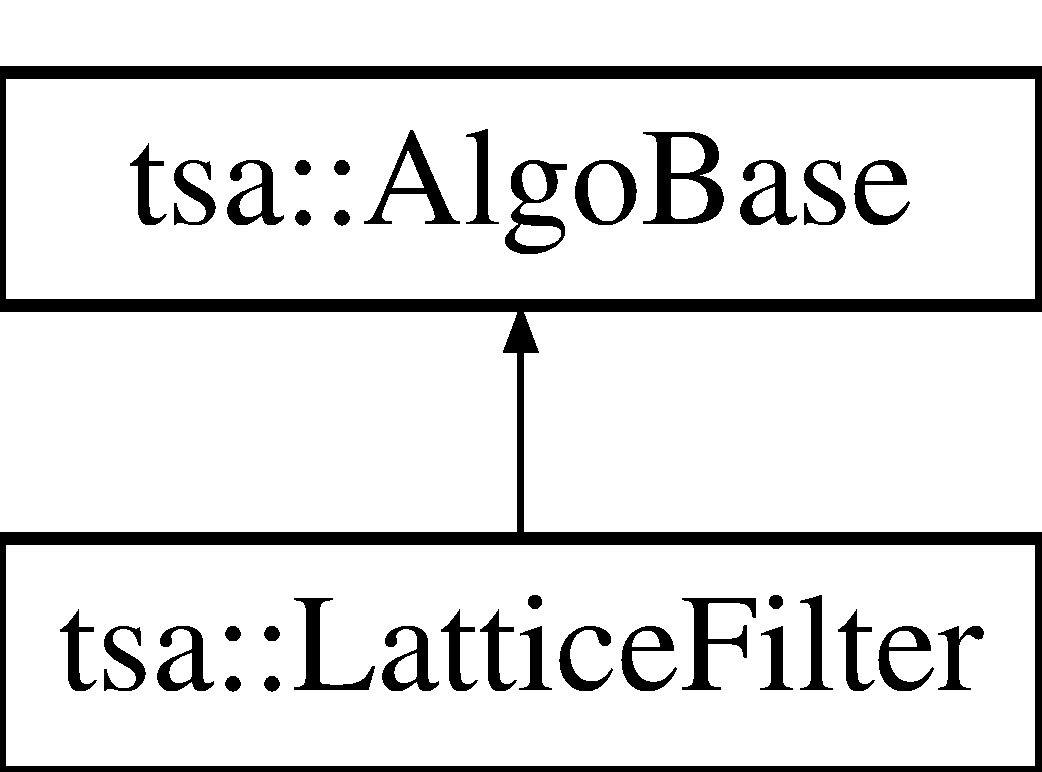
\includegraphics[height=2.000000cm]{classtsa_1_1_lattice_filter}
\end{center}
\end{figure}
\subsection*{Public Member Functions}
\begin{DoxyCompactItemize}
\item 
\hyperlink{classtsa_1_1_lattice_filter_a2cd66baf212f1b3824016c1e589b014a}{Lattice\+Filter} (\hyperlink{classtsa_1_1_lattice_view}{Lattice\+View} \&LV)
\item 
\hyperlink{classtsa_1_1_lattice_filter_af2e6c3e8d7fb7399f564f47c060bccc3}{Lattice\+Filter} (\hyperlink{namespacetsa_a8900fb03d849baf447a1a0efe2561fb2}{Dvector} \&ParcorF, \hyperlink{namespacetsa_a8900fb03d849baf447a1a0efe2561fb2}{Dvector} \&ParcorB, \hyperlink{namespacetsa_ad260cd21c1891c4ed391fe788569aba4}{Dmatrix} \&ErrF, \hyperlink{namespacetsa_ad260cd21c1891c4ed391fe788569aba4}{Dmatrix} \&ErrB)
\item 
virtual \hyperlink{classtsa_1_1_lattice_filter_a8a7c4763fe464837766a5beff88d36d5}{$\sim$\+Lattice\+Filter} ()
\item 
void \hyperlink{classtsa_1_1_lattice_filter_aa6be240d902449711c1925e464248a1d}{Load} (const char $\ast$filename, const char $\ast$fmt=\char`\"{}txt\char`\"{})
\item 
void \hyperlink{classtsa_1_1_lattice_filter_ac599ab3a2134d53e0685f91a0a673ed4}{Save} (const char $\ast$filename, const char $\ast$fmt=\char`\"{}txt\char`\"{})
\item 
void \hyperlink{classtsa_1_1_lattice_filter_ae9bd581cbcd1183a0dd7c557fe687422}{xml\+\_\+serialize} (\hyperlink{classeternity_1_1xml__archive}{eternity\+::xml\+\_\+archive} \&xml, const char $\ast$p)
\end{DoxyCompactItemize}
\begin{Indent}\textbf{ Operations}\par
\begin{DoxyCompactItemize}
\item 
void \hyperlink{classtsa_1_1_lattice_filter_a01071f8619620099315c1007c8980baf}{operator()} (\hyperlink{namespacetsa_ac599574bcc094eda25613724b8f3ca9e}{Seq\+View\+Double} \&Input\+Data, \hyperlink{namespacetsa_ac599574bcc094eda25613724b8f3ca9e}{Seq\+View\+Double} \&Whitened\+Data)
\item 
void \hyperlink{classtsa_1_1_lattice_filter_a08187ed236faefa36a0993190c6b0162}{init} (\hyperlink{classtsa_1_1_lattice_view}{Lattice\+View} \&LV)
\begin{DoxyCompactList}\small\item\em Initialization function. \end{DoxyCompactList}\item 
void \hyperlink{classtsa_1_1_lattice_filter_a09ebe977a54eed4453db605ab742f771}{execute} (matrix\+\_\+row$<$ \hyperlink{namespacetsa_ad260cd21c1891c4ed391fe788569aba4}{Dmatrix} $>$ Input, matrix\+\_\+row$<$ \hyperlink{namespacetsa_ad260cd21c1891c4ed391fe788569aba4}{Dmatrix} $>$ Output)
\begin{DoxyCompactList}\small\item\em The execute method implemts the filter in the lattice form. \end{DoxyCompactList}\end{DoxyCompactItemize}
\end{Indent}
\subsection*{Private Attributes}
\begin{DoxyCompactItemize}
\item 
unsigned int \hyperlink{classtsa_1_1_lattice_filter_aaff567ffb2c6b13538f138b8d49f3781}{m\+Order}
\item 
\hyperlink{namespacetsa_a8900fb03d849baf447a1a0efe2561fb2}{Dvector} \hyperlink{classtsa_1_1_lattice_filter_a4a7f9d6020bc4d7cab3d6021bd5338db}{m\+ParcorF}
\item 
\hyperlink{namespacetsa_a8900fb03d849baf447a1a0efe2561fb2}{Dvector} \hyperlink{classtsa_1_1_lattice_filter_a0e3a56f45a158477cef36e55cd2e5417}{m\+ParcorB}
\item 
\hyperlink{namespacetsa_ad260cd21c1891c4ed391fe788569aba4}{Dmatrix} \hyperlink{classtsa_1_1_lattice_filter_a462c5cd31c438a924bfde88d08e12200}{m\+ErrF}
\item 
\hyperlink{namespacetsa_ad260cd21c1891c4ed391fe788569aba4}{Dmatrix} \hyperlink{classtsa_1_1_lattice_filter_a0cd360b9836146c9296798337dd2ee0f}{m\+ErrB}
\item 
int \hyperlink{classtsa_1_1_lattice_filter_ab480cbe362a358df626bcd0758c0a7ce}{m\+Status}
\end{DoxyCompactItemize}


\subsection{Detailed Description}
Implement the lattice filter. 

Definition at line 77 of file Lattice\+Filter.\+hpp.



\subsection{Constructor \& Destructor Documentation}
\mbox{\Hypertarget{classtsa_1_1_lattice_filter_a2cd66baf212f1b3824016c1e589b014a}\label{classtsa_1_1_lattice_filter_a2cd66baf212f1b3824016c1e589b014a}} 
\index{tsa\+::\+Lattice\+Filter@{tsa\+::\+Lattice\+Filter}!Lattice\+Filter@{Lattice\+Filter}}
\index{Lattice\+Filter@{Lattice\+Filter}!tsa\+::\+Lattice\+Filter@{tsa\+::\+Lattice\+Filter}}
\subsubsection{\texorpdfstring{Lattice\+Filter()}{LatticeFilter()}\hspace{0.1cm}{\footnotesize\ttfamily [1/2]}}
{\footnotesize\ttfamily tsa\+::\+Lattice\+Filter\+::\+Lattice\+Filter (\begin{DoxyParamCaption}\item[{\hyperlink{classtsa_1_1_lattice_view}{Lattice\+View} \&}]{LV }\end{DoxyParamCaption})}

Constructor


\begin{DoxyParams}{Parameters}
{\em LV} & is the view containg the parameters for the Lattice Filter \\
\hline
\end{DoxyParams}
\begin{DoxyReturn}{Returns}

\end{DoxyReturn}


Definition at line 29 of file Lattice\+Filter.\+cpp.

\mbox{\Hypertarget{classtsa_1_1_lattice_filter_af2e6c3e8d7fb7399f564f47c060bccc3}\label{classtsa_1_1_lattice_filter_af2e6c3e8d7fb7399f564f47c060bccc3}} 
\index{tsa\+::\+Lattice\+Filter@{tsa\+::\+Lattice\+Filter}!Lattice\+Filter@{Lattice\+Filter}}
\index{Lattice\+Filter@{Lattice\+Filter}!tsa\+::\+Lattice\+Filter@{tsa\+::\+Lattice\+Filter}}
\subsubsection{\texorpdfstring{Lattice\+Filter()}{LatticeFilter()}\hspace{0.1cm}{\footnotesize\ttfamily [2/2]}}
{\footnotesize\ttfamily tsa\+::\+Lattice\+Filter\+::\+Lattice\+Filter (\begin{DoxyParamCaption}\item[{\hyperlink{namespacetsa_a8900fb03d849baf447a1a0efe2561fb2}{Dvector} \&}]{ParcorF,  }\item[{\hyperlink{namespacetsa_a8900fb03d849baf447a1a0efe2561fb2}{Dvector} \&}]{ParcorB,  }\item[{\hyperlink{namespacetsa_ad260cd21c1891c4ed391fe788569aba4}{Dmatrix} \&}]{ErrF,  }\item[{\hyperlink{namespacetsa_ad260cd21c1891c4ed391fe788569aba4}{Dmatrix} \&}]{ErrB }\end{DoxyParamCaption})}

Constructor 

Definition at line 19 of file Lattice\+Filter.\+cpp.

\mbox{\Hypertarget{classtsa_1_1_lattice_filter_a8a7c4763fe464837766a5beff88d36d5}\label{classtsa_1_1_lattice_filter_a8a7c4763fe464837766a5beff88d36d5}} 
\index{tsa\+::\+Lattice\+Filter@{tsa\+::\+Lattice\+Filter}!````~Lattice\+Filter@{$\sim$\+Lattice\+Filter}}
\index{````~Lattice\+Filter@{$\sim$\+Lattice\+Filter}!tsa\+::\+Lattice\+Filter@{tsa\+::\+Lattice\+Filter}}
\subsubsection{\texorpdfstring{$\sim$\+Lattice\+Filter()}{~LatticeFilter()}}
{\footnotesize\ttfamily tsa\+::\+Lattice\+Filter\+::$\sim$\+Lattice\+Filter (\begin{DoxyParamCaption}{ }\end{DoxyParamCaption})\hspace{0.3cm}{\ttfamily [virtual]}}

Destructor 

Definition at line 39 of file Lattice\+Filter.\+cpp.



\subsection{Member Function Documentation}
\mbox{\Hypertarget{classtsa_1_1_lattice_filter_a09ebe977a54eed4453db605ab742f771}\label{classtsa_1_1_lattice_filter_a09ebe977a54eed4453db605ab742f771}} 
\index{tsa\+::\+Lattice\+Filter@{tsa\+::\+Lattice\+Filter}!execute@{execute}}
\index{execute@{execute}!tsa\+::\+Lattice\+Filter@{tsa\+::\+Lattice\+Filter}}
\subsubsection{\texorpdfstring{execute()}{execute()}}
{\footnotesize\ttfamily void tsa\+::\+Lattice\+Filter\+::execute (\begin{DoxyParamCaption}\item[{matrix\+\_\+row$<$ \hyperlink{namespacetsa_ad260cd21c1891c4ed391fe788569aba4}{Dmatrix} $>$}]{Input,  }\item[{matrix\+\_\+row$<$ \hyperlink{namespacetsa_ad260cd21c1891c4ed391fe788569aba4}{Dmatrix} $>$}]{Output }\end{DoxyParamCaption})}



The execute method implemts the filter in the lattice form. 

\begin{DoxyPrecond}{Precondition}

\end{DoxyPrecond}
\begin{DoxyPostcond}{Postcondition}
A postcondition 
\end{DoxyPostcond}

\begin{DoxyExceptions}{Exceptions}
{\em An} & exception\\
\hline
\end{DoxyExceptions}
Declaration of execute operation


\begin{DoxyParams}{Parameters}
{\em Input} & is the input vector of data \\
\hline
{\em Output} & is the output (whitened) data \\
\hline
\end{DoxyParams}


Definition at line 51 of file Lattice\+Filter.\+cpp.

\mbox{\Hypertarget{classtsa_1_1_lattice_filter_a08187ed236faefa36a0993190c6b0162}\label{classtsa_1_1_lattice_filter_a08187ed236faefa36a0993190c6b0162}} 
\index{tsa\+::\+Lattice\+Filter@{tsa\+::\+Lattice\+Filter}!init@{init}}
\index{init@{init}!tsa\+::\+Lattice\+Filter@{tsa\+::\+Lattice\+Filter}}
\subsubsection{\texorpdfstring{init()}{init()}}
{\footnotesize\ttfamily void tsa\+::\+Lattice\+Filter\+::init (\begin{DoxyParamCaption}\item[{\hyperlink{classtsa_1_1_lattice_view}{Lattice\+View} \&}]{LV }\end{DoxyParamCaption})}



Initialization function. 


\begin{DoxyParams}{Parameters}
{\em LV} & lattice view \\
\hline
\end{DoxyParams}


Definition at line 42 of file Lattice\+Filter.\+cpp.

\mbox{\Hypertarget{classtsa_1_1_lattice_filter_aa6be240d902449711c1925e464248a1d}\label{classtsa_1_1_lattice_filter_aa6be240d902449711c1925e464248a1d}} 
\index{tsa\+::\+Lattice\+Filter@{tsa\+::\+Lattice\+Filter}!Load@{Load}}
\index{Load@{Load}!tsa\+::\+Lattice\+Filter@{tsa\+::\+Lattice\+Filter}}
\subsubsection{\texorpdfstring{Load()}{Load()}}
{\footnotesize\ttfamily void tsa\+::\+Lattice\+Filter\+::\+Load (\begin{DoxyParamCaption}\item[{const char $\ast$}]{filename,  }\item[{const char $\ast$}]{fmt = {\ttfamily \char`\"{}txt\char`\"{}} }\end{DoxyParamCaption})\hspace{0.3cm}{\ttfamily [inline]}}



Definition at line 98 of file Lattice\+Filter.\+hpp.

\mbox{\Hypertarget{classtsa_1_1_lattice_filter_a01071f8619620099315c1007c8980baf}\label{classtsa_1_1_lattice_filter_a01071f8619620099315c1007c8980baf}} 
\index{tsa\+::\+Lattice\+Filter@{tsa\+::\+Lattice\+Filter}!operator()@{operator()}}
\index{operator()@{operator()}!tsa\+::\+Lattice\+Filter@{tsa\+::\+Lattice\+Filter}}
\subsubsection{\texorpdfstring{operator()()}{operator()()}}
{\footnotesize\ttfamily void tsa\+::\+Lattice\+Filter\+::operator() (\begin{DoxyParamCaption}\item[{\hyperlink{namespacetsa_ac599574bcc094eda25613724b8f3ca9e}{Seq\+View\+Double} \&}]{Input\+Data,  }\item[{\hyperlink{namespacetsa_ac599574bcc094eda25613724b8f3ca9e}{Seq\+View\+Double} \&}]{Whitened\+Data }\end{DoxyParamCaption})\hspace{0.3cm}{\ttfamily [inline]}}

Declaration of execute operation


\begin{DoxyParams}{Parameters}
{\em Input\+Data} & Matrix containing Time Series \\
\hline
{\em Whitened\+Data} & Matrix containing the Whitened\+Data \\
\hline
\end{DoxyParams}


Definition at line 163 of file Lattice\+Filter.\+hpp.

\mbox{\Hypertarget{classtsa_1_1_lattice_filter_ac599ab3a2134d53e0685f91a0a673ed4}\label{classtsa_1_1_lattice_filter_ac599ab3a2134d53e0685f91a0a673ed4}} 
\index{tsa\+::\+Lattice\+Filter@{tsa\+::\+Lattice\+Filter}!Save@{Save}}
\index{Save@{Save}!tsa\+::\+Lattice\+Filter@{tsa\+::\+Lattice\+Filter}}
\subsubsection{\texorpdfstring{Save()}{Save()}}
{\footnotesize\ttfamily void tsa\+::\+Lattice\+Filter\+::\+Save (\begin{DoxyParamCaption}\item[{const char $\ast$}]{filename,  }\item[{const char $\ast$}]{fmt = {\ttfamily \char`\"{}txt\char`\"{}} }\end{DoxyParamCaption})\hspace{0.3cm}{\ttfamily [inline]}}



Definition at line 105 of file Lattice\+Filter.\+hpp.

\mbox{\Hypertarget{classtsa_1_1_lattice_filter_ae9bd581cbcd1183a0dd7c557fe687422}\label{classtsa_1_1_lattice_filter_ae9bd581cbcd1183a0dd7c557fe687422}} 
\index{tsa\+::\+Lattice\+Filter@{tsa\+::\+Lattice\+Filter}!xml\+\_\+serialize@{xml\+\_\+serialize}}
\index{xml\+\_\+serialize@{xml\+\_\+serialize}!tsa\+::\+Lattice\+Filter@{tsa\+::\+Lattice\+Filter}}
\subsubsection{\texorpdfstring{xml\+\_\+serialize()}{xml\_serialize()}}
{\footnotesize\ttfamily void tsa\+::\+Lattice\+Filter\+::xml\+\_\+serialize (\begin{DoxyParamCaption}\item[{\hyperlink{classeternity_1_1xml__archive}{eternity\+::xml\+\_\+archive} \&}]{xml,  }\item[{const char $\ast$}]{p }\end{DoxyParamCaption})\hspace{0.3cm}{\ttfamily [inline]}}



Definition at line 112 of file Lattice\+Filter.\+hpp.



\subsection{Member Data Documentation}
\mbox{\Hypertarget{classtsa_1_1_lattice_filter_a0cd360b9836146c9296798337dd2ee0f}\label{classtsa_1_1_lattice_filter_a0cd360b9836146c9296798337dd2ee0f}} 
\index{tsa\+::\+Lattice\+Filter@{tsa\+::\+Lattice\+Filter}!m\+ErrB@{m\+ErrB}}
\index{m\+ErrB@{m\+ErrB}!tsa\+::\+Lattice\+Filter@{tsa\+::\+Lattice\+Filter}}
\subsubsection{\texorpdfstring{m\+ErrB}{mErrB}}
{\footnotesize\ttfamily \hyperlink{namespacetsa_ad260cd21c1891c4ed391fe788569aba4}{Dmatrix} tsa\+::\+Lattice\+Filter\+::m\+ErrB\hspace{0.3cm}{\ttfamily [private]}}



Definition at line 225 of file Lattice\+Filter.\+hpp.

\mbox{\Hypertarget{classtsa_1_1_lattice_filter_a462c5cd31c438a924bfde88d08e12200}\label{classtsa_1_1_lattice_filter_a462c5cd31c438a924bfde88d08e12200}} 
\index{tsa\+::\+Lattice\+Filter@{tsa\+::\+Lattice\+Filter}!m\+ErrF@{m\+ErrF}}
\index{m\+ErrF@{m\+ErrF}!tsa\+::\+Lattice\+Filter@{tsa\+::\+Lattice\+Filter}}
\subsubsection{\texorpdfstring{m\+ErrF}{mErrF}}
{\footnotesize\ttfamily \hyperlink{namespacetsa_ad260cd21c1891c4ed391fe788569aba4}{Dmatrix} tsa\+::\+Lattice\+Filter\+::m\+ErrF\hspace{0.3cm}{\ttfamily [private]}}



Definition at line 224 of file Lattice\+Filter.\+hpp.

\mbox{\Hypertarget{classtsa_1_1_lattice_filter_aaff567ffb2c6b13538f138b8d49f3781}\label{classtsa_1_1_lattice_filter_aaff567ffb2c6b13538f138b8d49f3781}} 
\index{tsa\+::\+Lattice\+Filter@{tsa\+::\+Lattice\+Filter}!m\+Order@{m\+Order}}
\index{m\+Order@{m\+Order}!tsa\+::\+Lattice\+Filter@{tsa\+::\+Lattice\+Filter}}
\subsubsection{\texorpdfstring{m\+Order}{mOrder}}
{\footnotesize\ttfamily unsigned int tsa\+::\+Lattice\+Filter\+::m\+Order\hspace{0.3cm}{\ttfamily [private]}}



Definition at line 221 of file Lattice\+Filter.\+hpp.

\mbox{\Hypertarget{classtsa_1_1_lattice_filter_a0e3a56f45a158477cef36e55cd2e5417}\label{classtsa_1_1_lattice_filter_a0e3a56f45a158477cef36e55cd2e5417}} 
\index{tsa\+::\+Lattice\+Filter@{tsa\+::\+Lattice\+Filter}!m\+ParcorB@{m\+ParcorB}}
\index{m\+ParcorB@{m\+ParcorB}!tsa\+::\+Lattice\+Filter@{tsa\+::\+Lattice\+Filter}}
\subsubsection{\texorpdfstring{m\+ParcorB}{mParcorB}}
{\footnotesize\ttfamily \hyperlink{namespacetsa_a8900fb03d849baf447a1a0efe2561fb2}{Dvector} tsa\+::\+Lattice\+Filter\+::m\+ParcorB\hspace{0.3cm}{\ttfamily [private]}}



Definition at line 223 of file Lattice\+Filter.\+hpp.

\mbox{\Hypertarget{classtsa_1_1_lattice_filter_a4a7f9d6020bc4d7cab3d6021bd5338db}\label{classtsa_1_1_lattice_filter_a4a7f9d6020bc4d7cab3d6021bd5338db}} 
\index{tsa\+::\+Lattice\+Filter@{tsa\+::\+Lattice\+Filter}!m\+ParcorF@{m\+ParcorF}}
\index{m\+ParcorF@{m\+ParcorF}!tsa\+::\+Lattice\+Filter@{tsa\+::\+Lattice\+Filter}}
\subsubsection{\texorpdfstring{m\+ParcorF}{mParcorF}}
{\footnotesize\ttfamily \hyperlink{namespacetsa_a8900fb03d849baf447a1a0efe2561fb2}{Dvector} tsa\+::\+Lattice\+Filter\+::m\+ParcorF\hspace{0.3cm}{\ttfamily [private]}}



Definition at line 222 of file Lattice\+Filter.\+hpp.

\mbox{\Hypertarget{classtsa_1_1_lattice_filter_ab480cbe362a358df626bcd0758c0a7ce}\label{classtsa_1_1_lattice_filter_ab480cbe362a358df626bcd0758c0a7ce}} 
\index{tsa\+::\+Lattice\+Filter@{tsa\+::\+Lattice\+Filter}!m\+Status@{m\+Status}}
\index{m\+Status@{m\+Status}!tsa\+::\+Lattice\+Filter@{tsa\+::\+Lattice\+Filter}}
\subsubsection{\texorpdfstring{m\+Status}{mStatus}}
{\footnotesize\ttfamily int tsa\+::\+Lattice\+Filter\+::m\+Status\hspace{0.3cm}{\ttfamily [private]}}



Definition at line 226 of file Lattice\+Filter.\+hpp.



The documentation for this class was generated from the following files\+:\begin{DoxyCompactItemize}
\item 
/home/filip/\+Ph\+D/\+W\+D\+F\+Pipe\+\_\+test/p4\+T\+S\+A/include/\hyperlink{_lattice_filter_8hpp}{Lattice\+Filter.\+hpp}\item 
/home/filip/\+Ph\+D/\+W\+D\+F\+Pipe\+\_\+test/p4\+T\+S\+A/src/\hyperlink{_lattice_filter_8cpp}{Lattice\+Filter.\+cpp}\end{DoxyCompactItemize}

\hypertarget{classtsa_1_1_lattice_view}{}\section{tsa\+:\+:Lattice\+View Class Reference}
\label{classtsa_1_1_lattice_view}\index{tsa\+::\+Lattice\+View@{tsa\+::\+Lattice\+View}}


Define the object needed to implement the Lattice filter.  




{\ttfamily \#include $<$Lattice\+View.\+hpp$>$}

Inheritance diagram for tsa\+:\+:Lattice\+View\+:\begin{figure}[H]
\begin{center}
\leavevmode
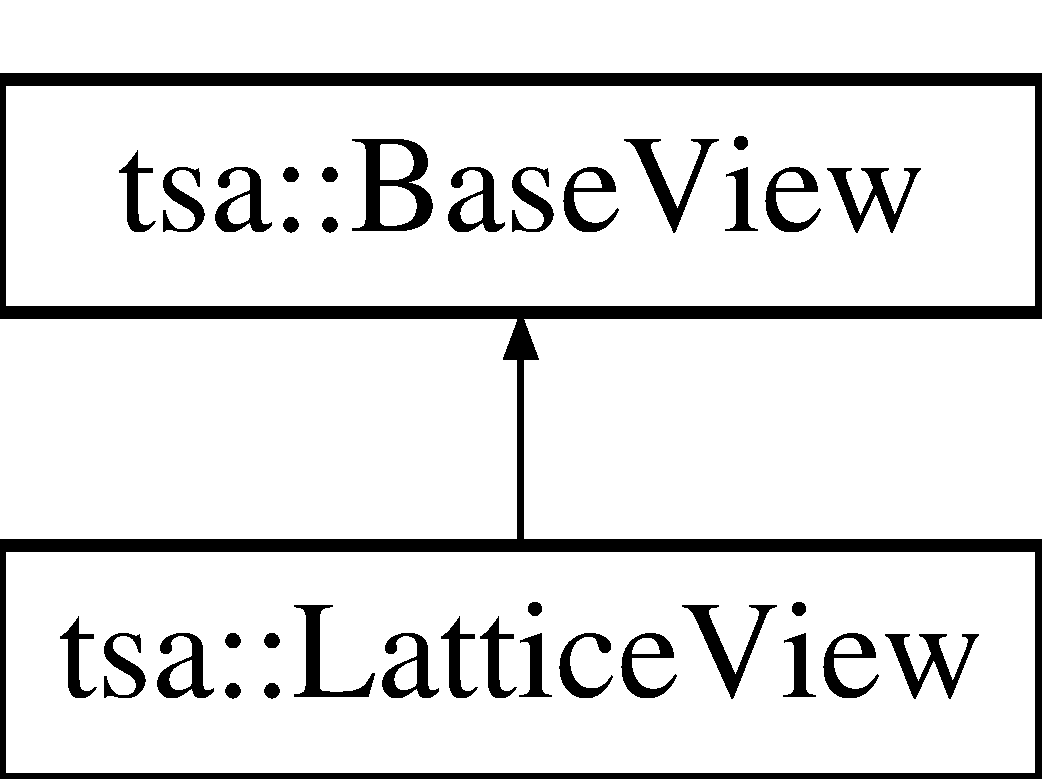
\includegraphics[height=2.000000cm]{classtsa_1_1_lattice_view}
\end{center}
\end{figure}
\subsection*{Public Member Functions}
\begin{DoxyCompactItemize}
\item 
\hyperlink{classtsa_1_1_lattice_view_ab06c208ec07241d525afa95112a49a61}{Lattice\+View} (unsigned int Ar\+Order=1)
\item 
\hyperlink{classtsa_1_1_lattice_view_a2c5158bb8d09c4742906a4eb1c2b8caf}{$\sim$\+Lattice\+View} ()
\item 
void \hyperlink{classtsa_1_1_lattice_view_a4a8f6b4faf4a5c61cbd66aab056e18ab}{Load} (const char $\ast$filename, const char $\ast$fmt=\char`\"{}txt\char`\"{})
\item 
void \hyperlink{classtsa_1_1_lattice_view_a911eefc09c14ed78dee42fffe237ac3a}{Save} (const char $\ast$filename, const char $\ast$fmt=\char`\"{}txt\char`\"{})
\item 
void \hyperlink{classtsa_1_1_lattice_view_a9040c52c4481b0e47346aa39f150c3b2}{xml\+\_\+serialize} (\hyperlink{classeternity_1_1xml__archive}{eternity\+::xml\+\_\+archive} \&xml, const char $\ast$prefix)
\end{DoxyCompactItemize}
\begin{Indent}\textbf{ Getters}\par
\begin{DoxyCompactItemize}
\item 
unsigned int \hyperlink{classtsa_1_1_lattice_view_a9aedf999a2129ae0b000ba6caded4b6b}{Get\+Order} ()
\item 
double \hyperlink{classtsa_1_1_lattice_view_a0549c29576047fa4e0c4871a23904951}{Get\+Parcor} (unsigned int j)
\item 
\hyperlink{namespacetsa_a8900fb03d849baf447a1a0efe2561fb2}{Dvector} $\ast$ \hyperlink{classtsa_1_1_lattice_view_a302999b98f7af945965749026dc655f9}{Get\+ParcorF} ()
\item 
\hyperlink{namespacetsa_a8900fb03d849baf447a1a0efe2561fb2}{Dvector} $\ast$ \hyperlink{classtsa_1_1_lattice_view_a166491c83511a3c64ec63c1aa5e2cbbd}{Get\+ParcorB} ()
\item 
double \hyperlink{classtsa_1_1_lattice_view_a941542e69cf15f8a41cfc17253cd5d48}{Get\+ParcorF} (unsigned int j)
\item 
double \hyperlink{classtsa_1_1_lattice_view_a14148e7fdd220c61791732bc14130bd9}{Get\+ParcorB} (unsigned int j)
\item 
\hyperlink{namespacetsa_ad260cd21c1891c4ed391fe788569aba4}{Dmatrix} $\ast$ \hyperlink{classtsa_1_1_lattice_view_a893dd18c7f1d423a8478a786c3c731c5}{Get\+Error\+Forward} ()
\item 
\hyperlink{namespacetsa_ad260cd21c1891c4ed391fe788569aba4}{Dmatrix} $\ast$ \hyperlink{classtsa_1_1_lattice_view_a8b682c3db5bcce323d107e4ba889795f}{Get\+Error\+Backward} ()
\item 
double \hyperlink{classtsa_1_1_lattice_view_ac9a4c9e01891d9c7c2ba5139c23ac86e}{Get\+Error\+Forward} (unsigned int i, unsigned int j)
\item 
double \hyperlink{classtsa_1_1_lattice_view_ae0bdb3cfb70274cf21c8681393d92a45}{Get\+Error\+Backward} (unsigned int i, unsigned int j)
\end{DoxyCompactItemize}
\end{Indent}
\begin{Indent}\textbf{ Setters}\par
\begin{DoxyCompactItemize}
\item 
void \hyperlink{classtsa_1_1_lattice_view_a0d555a7ff35604537e4391d4debd2d9a}{Set\+Order} (unsigned int v)
\item 
void \hyperlink{classtsa_1_1_lattice_view_a0e099a0196edb96d4e9265ea2901e6b9}{Set\+ParcorF} (unsigned int j, double v)
\item 
void \hyperlink{classtsa_1_1_lattice_view_ae2bb756238fc6873839459097717f3dc}{Set\+ParcorB} (unsigned int j, double v)
\item 
void \hyperlink{classtsa_1_1_lattice_view_a5d40a6a9e27b0ede53e2735983a83c6e}{Set\+Error\+Forward} (unsigned int j, double v)
\item 
void \hyperlink{classtsa_1_1_lattice_view_a80b37195a303625d69009cba7f8a0156}{Set\+Error\+Backward} (unsigned int j, double v)
\end{DoxyCompactItemize}
\end{Indent}
\subsection*{Private Attributes}
\begin{DoxyCompactItemize}
\item 
unsigned int \hyperlink{classtsa_1_1_lattice_view_acb69a220044c95ee2b32d90ce4ee2f7c}{m\+Order}
\begin{DoxyCompactList}\small\item\em the Order of the View \end{DoxyCompactList}\item 
\hyperlink{namespacetsa_ad260cd21c1891c4ed391fe788569aba4}{Dmatrix} \hyperlink{classtsa_1_1_lattice_view_ac7976d0ac256453229dec51c14da0c26}{m\+Error\+Forward}
\begin{DoxyCompactList}\small\item\em the Error Forward for the Lattice Filter \end{DoxyCompactList}\item 
\hyperlink{namespacetsa_ad260cd21c1891c4ed391fe788569aba4}{Dmatrix} \hyperlink{classtsa_1_1_lattice_view_a9bbdb82e6aee17385ed9cd45da26c6ea}{m\+Error\+Backward}
\begin{DoxyCompactList}\small\item\em the Error Backward for the Lattice Filter \end{DoxyCompactList}\item 
\hyperlink{namespacetsa_a8900fb03d849baf447a1a0efe2561fb2}{Dvector} \hyperlink{classtsa_1_1_lattice_view_a3fbd93734d9b37488687840609c93e7a}{m\+ParcorF}
\begin{DoxyCompactList}\small\item\em the vector of forward Parcor \end{DoxyCompactList}\item 
\hyperlink{namespacetsa_a8900fb03d849baf447a1a0efe2561fb2}{Dvector} \hyperlink{classtsa_1_1_lattice_view_a07aba04a75f98622d97ef4baac7a95e6}{m\+ParcorB}
\begin{DoxyCompactList}\small\item\em the vector of backward Parcor \end{DoxyCompactList}\end{DoxyCompactItemize}
\subsection*{Additional Inherited Members}


\subsection{Detailed Description}
Define the object needed to implement the Lattice filter. 

Definition at line 75 of file Lattice\+View.\+hpp.



\subsection{Constructor \& Destructor Documentation}
\mbox{\Hypertarget{classtsa_1_1_lattice_view_ab06c208ec07241d525afa95112a49a61}\label{classtsa_1_1_lattice_view_ab06c208ec07241d525afa95112a49a61}} 
\index{tsa\+::\+Lattice\+View@{tsa\+::\+Lattice\+View}!Lattice\+View@{Lattice\+View}}
\index{Lattice\+View@{Lattice\+View}!tsa\+::\+Lattice\+View@{tsa\+::\+Lattice\+View}}
\subsubsection{\texorpdfstring{Lattice\+View()}{LatticeView()}}
{\footnotesize\ttfamily tsa\+::\+Lattice\+View\+::\+Lattice\+View (\begin{DoxyParamCaption}\item[{unsigned int}]{Ar\+Order = {\ttfamily 1} }\end{DoxyParamCaption})\hspace{0.3cm}{\ttfamily [inline]}}

Constructor 

Definition at line 81 of file Lattice\+View.\+hpp.

\mbox{\Hypertarget{classtsa_1_1_lattice_view_a2c5158bb8d09c4742906a4eb1c2b8caf}\label{classtsa_1_1_lattice_view_a2c5158bb8d09c4742906a4eb1c2b8caf}} 
\index{tsa\+::\+Lattice\+View@{tsa\+::\+Lattice\+View}!````~Lattice\+View@{$\sim$\+Lattice\+View}}
\index{````~Lattice\+View@{$\sim$\+Lattice\+View}!tsa\+::\+Lattice\+View@{tsa\+::\+Lattice\+View}}
\subsubsection{\texorpdfstring{$\sim$\+Lattice\+View()}{~LatticeView()}}
{\footnotesize\ttfamily tsa\+::\+Lattice\+View\+::$\sim$\+Lattice\+View (\begin{DoxyParamCaption}{ }\end{DoxyParamCaption})\hspace{0.3cm}{\ttfamily [inline]}}



Definition at line 96 of file Lattice\+View.\+hpp.



\subsection{Member Function Documentation}
\mbox{\Hypertarget{classtsa_1_1_lattice_view_a8b682c3db5bcce323d107e4ba889795f}\label{classtsa_1_1_lattice_view_a8b682c3db5bcce323d107e4ba889795f}} 
\index{tsa\+::\+Lattice\+View@{tsa\+::\+Lattice\+View}!Get\+Error\+Backward@{Get\+Error\+Backward}}
\index{Get\+Error\+Backward@{Get\+Error\+Backward}!tsa\+::\+Lattice\+View@{tsa\+::\+Lattice\+View}}
\subsubsection{\texorpdfstring{Get\+Error\+Backward()}{GetErrorBackward()}\hspace{0.1cm}{\footnotesize\ttfamily [1/2]}}
{\footnotesize\ttfamily \hyperlink{namespacetsa_ad260cd21c1891c4ed391fe788569aba4}{Dmatrix}$\ast$ tsa\+::\+Lattice\+View\+::\+Get\+Error\+Backward (\begin{DoxyParamCaption}{ }\end{DoxyParamCaption})\hspace{0.3cm}{\ttfamily [inline]}}



Definition at line 201 of file Lattice\+View.\+hpp.

\mbox{\Hypertarget{classtsa_1_1_lattice_view_ae0bdb3cfb70274cf21c8681393d92a45}\label{classtsa_1_1_lattice_view_ae0bdb3cfb70274cf21c8681393d92a45}} 
\index{tsa\+::\+Lattice\+View@{tsa\+::\+Lattice\+View}!Get\+Error\+Backward@{Get\+Error\+Backward}}
\index{Get\+Error\+Backward@{Get\+Error\+Backward}!tsa\+::\+Lattice\+View@{tsa\+::\+Lattice\+View}}
\subsubsection{\texorpdfstring{Get\+Error\+Backward()}{GetErrorBackward()}\hspace{0.1cm}{\footnotesize\ttfamily [2/2]}}
{\footnotesize\ttfamily double tsa\+::\+Lattice\+View\+::\+Get\+Error\+Backward (\begin{DoxyParamCaption}\item[{unsigned int}]{i,  }\item[{unsigned int}]{j }\end{DoxyParamCaption})\hspace{0.3cm}{\ttfamily [inline]}}



Definition at line 217 of file Lattice\+View.\+hpp.

\mbox{\Hypertarget{classtsa_1_1_lattice_view_a893dd18c7f1d423a8478a786c3c731c5}\label{classtsa_1_1_lattice_view_a893dd18c7f1d423a8478a786c3c731c5}} 
\index{tsa\+::\+Lattice\+View@{tsa\+::\+Lattice\+View}!Get\+Error\+Forward@{Get\+Error\+Forward}}
\index{Get\+Error\+Forward@{Get\+Error\+Forward}!tsa\+::\+Lattice\+View@{tsa\+::\+Lattice\+View}}
\subsubsection{\texorpdfstring{Get\+Error\+Forward()}{GetErrorForward()}\hspace{0.1cm}{\footnotesize\ttfamily [1/2]}}
{\footnotesize\ttfamily \hyperlink{namespacetsa_ad260cd21c1891c4ed391fe788569aba4}{Dmatrix}$\ast$ tsa\+::\+Lattice\+View\+::\+Get\+Error\+Forward (\begin{DoxyParamCaption}{ }\end{DoxyParamCaption})\hspace{0.3cm}{\ttfamily [inline]}}



Definition at line 197 of file Lattice\+View.\+hpp.

\mbox{\Hypertarget{classtsa_1_1_lattice_view_ac9a4c9e01891d9c7c2ba5139c23ac86e}\label{classtsa_1_1_lattice_view_ac9a4c9e01891d9c7c2ba5139c23ac86e}} 
\index{tsa\+::\+Lattice\+View@{tsa\+::\+Lattice\+View}!Get\+Error\+Forward@{Get\+Error\+Forward}}
\index{Get\+Error\+Forward@{Get\+Error\+Forward}!tsa\+::\+Lattice\+View@{tsa\+::\+Lattice\+View}}
\subsubsection{\texorpdfstring{Get\+Error\+Forward()}{GetErrorForward()}\hspace{0.1cm}{\footnotesize\ttfamily [2/2]}}
{\footnotesize\ttfamily double tsa\+::\+Lattice\+View\+::\+Get\+Error\+Forward (\begin{DoxyParamCaption}\item[{unsigned int}]{i,  }\item[{unsigned int}]{j }\end{DoxyParamCaption})\hspace{0.3cm}{\ttfamily [inline]}}



Definition at line 210 of file Lattice\+View.\+hpp.

\mbox{\Hypertarget{classtsa_1_1_lattice_view_a9aedf999a2129ae0b000ba6caded4b6b}\label{classtsa_1_1_lattice_view_a9aedf999a2129ae0b000ba6caded4b6b}} 
\index{tsa\+::\+Lattice\+View@{tsa\+::\+Lattice\+View}!Get\+Order@{Get\+Order}}
\index{Get\+Order@{Get\+Order}!tsa\+::\+Lattice\+View@{tsa\+::\+Lattice\+View}}
\subsubsection{\texorpdfstring{Get\+Order()}{GetOrder()}}
{\footnotesize\ttfamily unsigned int tsa\+::\+Lattice\+View\+::\+Get\+Order (\begin{DoxyParamCaption}{ }\end{DoxyParamCaption})\hspace{0.3cm}{\ttfamily [inline]}}

\begin{DoxyReturn}{Returns}
Order of the \hyperlink{classtsa_1_1_lattice_view}{Lattice\+View} 
\end{DoxyReturn}


Definition at line 153 of file Lattice\+View.\+hpp.

\mbox{\Hypertarget{classtsa_1_1_lattice_view_a0549c29576047fa4e0c4871a23904951}\label{classtsa_1_1_lattice_view_a0549c29576047fa4e0c4871a23904951}} 
\index{tsa\+::\+Lattice\+View@{tsa\+::\+Lattice\+View}!Get\+Parcor@{Get\+Parcor}}
\index{Get\+Parcor@{Get\+Parcor}!tsa\+::\+Lattice\+View@{tsa\+::\+Lattice\+View}}
\subsubsection{\texorpdfstring{Get\+Parcor()}{GetParcor()}}
{\footnotesize\ttfamily double tsa\+::\+Lattice\+View\+::\+Get\+Parcor (\begin{DoxyParamCaption}\item[{unsigned int}]{j }\end{DoxyParamCaption})\hspace{0.3cm}{\ttfamily [inline]}}


\begin{DoxyParams}{Parameters}
{\em j} & index of the vector \\
\hline
\end{DoxyParams}
\begin{DoxyReturn}{Returns}
The Parcor parameter 
\end{DoxyReturn}


Definition at line 164 of file Lattice\+View.\+hpp.

\mbox{\Hypertarget{classtsa_1_1_lattice_view_a166491c83511a3c64ec63c1aa5e2cbbd}\label{classtsa_1_1_lattice_view_a166491c83511a3c64ec63c1aa5e2cbbd}} 
\index{tsa\+::\+Lattice\+View@{tsa\+::\+Lattice\+View}!Get\+ParcorB@{Get\+ParcorB}}
\index{Get\+ParcorB@{Get\+ParcorB}!tsa\+::\+Lattice\+View@{tsa\+::\+Lattice\+View}}
\subsubsection{\texorpdfstring{Get\+Parcor\+B()}{GetParcorB()}\hspace{0.1cm}{\footnotesize\ttfamily [1/2]}}
{\footnotesize\ttfamily \hyperlink{namespacetsa_a8900fb03d849baf447a1a0efe2561fb2}{Dvector}$\ast$ tsa\+::\+Lattice\+View\+::\+Get\+ParcorB (\begin{DoxyParamCaption}{ }\end{DoxyParamCaption})\hspace{0.3cm}{\ttfamily [inline]}}



Definition at line 173 of file Lattice\+View.\+hpp.

\mbox{\Hypertarget{classtsa_1_1_lattice_view_a14148e7fdd220c61791732bc14130bd9}\label{classtsa_1_1_lattice_view_a14148e7fdd220c61791732bc14130bd9}} 
\index{tsa\+::\+Lattice\+View@{tsa\+::\+Lattice\+View}!Get\+ParcorB@{Get\+ParcorB}}
\index{Get\+ParcorB@{Get\+ParcorB}!tsa\+::\+Lattice\+View@{tsa\+::\+Lattice\+View}}
\subsubsection{\texorpdfstring{Get\+Parcor\+B()}{GetParcorB()}\hspace{0.1cm}{\footnotesize\ttfamily [2/2]}}
{\footnotesize\ttfamily double tsa\+::\+Lattice\+View\+::\+Get\+ParcorB (\begin{DoxyParamCaption}\item[{unsigned int}]{j }\end{DoxyParamCaption})\hspace{0.3cm}{\ttfamily [inline]}}


\begin{DoxyParams}{Parameters}
{\em j} & index of the vector \\
\hline
\end{DoxyParams}
\begin{DoxyReturn}{Returns}
The Parcor parameter 
\end{DoxyReturn}


Definition at line 193 of file Lattice\+View.\+hpp.

\mbox{\Hypertarget{classtsa_1_1_lattice_view_a302999b98f7af945965749026dc655f9}\label{classtsa_1_1_lattice_view_a302999b98f7af945965749026dc655f9}} 
\index{tsa\+::\+Lattice\+View@{tsa\+::\+Lattice\+View}!Get\+ParcorF@{Get\+ParcorF}}
\index{Get\+ParcorF@{Get\+ParcorF}!tsa\+::\+Lattice\+View@{tsa\+::\+Lattice\+View}}
\subsubsection{\texorpdfstring{Get\+Parcor\+F()}{GetParcorF()}\hspace{0.1cm}{\footnotesize\ttfamily [1/2]}}
{\footnotesize\ttfamily \hyperlink{namespacetsa_a8900fb03d849baf447a1a0efe2561fb2}{Dvector}$\ast$ tsa\+::\+Lattice\+View\+::\+Get\+ParcorF (\begin{DoxyParamCaption}{ }\end{DoxyParamCaption})\hspace{0.3cm}{\ttfamily [inline]}}



Definition at line 169 of file Lattice\+View.\+hpp.

\mbox{\Hypertarget{classtsa_1_1_lattice_view_a941542e69cf15f8a41cfc17253cd5d48}\label{classtsa_1_1_lattice_view_a941542e69cf15f8a41cfc17253cd5d48}} 
\index{tsa\+::\+Lattice\+View@{tsa\+::\+Lattice\+View}!Get\+ParcorF@{Get\+ParcorF}}
\index{Get\+ParcorF@{Get\+ParcorF}!tsa\+::\+Lattice\+View@{tsa\+::\+Lattice\+View}}
\subsubsection{\texorpdfstring{Get\+Parcor\+F()}{GetParcorF()}\hspace{0.1cm}{\footnotesize\ttfamily [2/2]}}
{\footnotesize\ttfamily double tsa\+::\+Lattice\+View\+::\+Get\+ParcorF (\begin{DoxyParamCaption}\item[{unsigned int}]{j }\end{DoxyParamCaption})\hspace{0.3cm}{\ttfamily [inline]}}


\begin{DoxyParams}{Parameters}
{\em j} & index of the vector \\
\hline
\end{DoxyParams}
\begin{DoxyReturn}{Returns}
The Parcor parameter 
\end{DoxyReturn}


Definition at line 183 of file Lattice\+View.\+hpp.

\mbox{\Hypertarget{classtsa_1_1_lattice_view_a4a8f6b4faf4a5c61cbd66aab056e18ab}\label{classtsa_1_1_lattice_view_a4a8f6b4faf4a5c61cbd66aab056e18ab}} 
\index{tsa\+::\+Lattice\+View@{tsa\+::\+Lattice\+View}!Load@{Load}}
\index{Load@{Load}!tsa\+::\+Lattice\+View@{tsa\+::\+Lattice\+View}}
\subsubsection{\texorpdfstring{Load()}{Load()}}
{\footnotesize\ttfamily void tsa\+::\+Lattice\+View\+::\+Load (\begin{DoxyParamCaption}\item[{const char $\ast$}]{filename,  }\item[{const char $\ast$}]{fmt = {\ttfamily \char`\"{}txt\char`\"{}} }\end{DoxyParamCaption})\hspace{0.3cm}{\ttfamily [inline]}}



Definition at line 99 of file Lattice\+View.\+hpp.

\mbox{\Hypertarget{classtsa_1_1_lattice_view_a911eefc09c14ed78dee42fffe237ac3a}\label{classtsa_1_1_lattice_view_a911eefc09c14ed78dee42fffe237ac3a}} 
\index{tsa\+::\+Lattice\+View@{tsa\+::\+Lattice\+View}!Save@{Save}}
\index{Save@{Save}!tsa\+::\+Lattice\+View@{tsa\+::\+Lattice\+View}}
\subsubsection{\texorpdfstring{Save()}{Save()}}
{\footnotesize\ttfamily void tsa\+::\+Lattice\+View\+::\+Save (\begin{DoxyParamCaption}\item[{const char $\ast$}]{filename,  }\item[{const char $\ast$}]{fmt = {\ttfamily \char`\"{}txt\char`\"{}} }\end{DoxyParamCaption})\hspace{0.3cm}{\ttfamily [inline]}}



Definition at line 106 of file Lattice\+View.\+hpp.

\mbox{\Hypertarget{classtsa_1_1_lattice_view_a80b37195a303625d69009cba7f8a0156}\label{classtsa_1_1_lattice_view_a80b37195a303625d69009cba7f8a0156}} 
\index{tsa\+::\+Lattice\+View@{tsa\+::\+Lattice\+View}!Set\+Error\+Backward@{Set\+Error\+Backward}}
\index{Set\+Error\+Backward@{Set\+Error\+Backward}!tsa\+::\+Lattice\+View@{tsa\+::\+Lattice\+View}}
\subsubsection{\texorpdfstring{Set\+Error\+Backward()}{SetErrorBackward()}}
{\footnotesize\ttfamily void tsa\+::\+Lattice\+View\+::\+Set\+Error\+Backward (\begin{DoxyParamCaption}\item[{unsigned int}]{j,  }\item[{double}]{v }\end{DoxyParamCaption})\hspace{0.3cm}{\ttfamily [inline]}}



Definition at line 246 of file Lattice\+View.\+hpp.

\mbox{\Hypertarget{classtsa_1_1_lattice_view_a5d40a6a9e27b0ede53e2735983a83c6e}\label{classtsa_1_1_lattice_view_a5d40a6a9e27b0ede53e2735983a83c6e}} 
\index{tsa\+::\+Lattice\+View@{tsa\+::\+Lattice\+View}!Set\+Error\+Forward@{Set\+Error\+Forward}}
\index{Set\+Error\+Forward@{Set\+Error\+Forward}!tsa\+::\+Lattice\+View@{tsa\+::\+Lattice\+View}}
\subsubsection{\texorpdfstring{Set\+Error\+Forward()}{SetErrorForward()}}
{\footnotesize\ttfamily void tsa\+::\+Lattice\+View\+::\+Set\+Error\+Forward (\begin{DoxyParamCaption}\item[{unsigned int}]{j,  }\item[{double}]{v }\end{DoxyParamCaption})\hspace{0.3cm}{\ttfamily [inline]}}



Definition at line 241 of file Lattice\+View.\+hpp.

\mbox{\Hypertarget{classtsa_1_1_lattice_view_a0d555a7ff35604537e4391d4debd2d9a}\label{classtsa_1_1_lattice_view_a0d555a7ff35604537e4391d4debd2d9a}} 
\index{tsa\+::\+Lattice\+View@{tsa\+::\+Lattice\+View}!Set\+Order@{Set\+Order}}
\index{Set\+Order@{Set\+Order}!tsa\+::\+Lattice\+View@{tsa\+::\+Lattice\+View}}
\subsubsection{\texorpdfstring{Set\+Order()}{SetOrder()}}
{\footnotesize\ttfamily void tsa\+::\+Lattice\+View\+::\+Set\+Order (\begin{DoxyParamCaption}\item[{unsigned int}]{v }\end{DoxyParamCaption})\hspace{0.3cm}{\ttfamily [inline]}}



Definition at line 229 of file Lattice\+View.\+hpp.

\mbox{\Hypertarget{classtsa_1_1_lattice_view_ae2bb756238fc6873839459097717f3dc}\label{classtsa_1_1_lattice_view_ae2bb756238fc6873839459097717f3dc}} 
\index{tsa\+::\+Lattice\+View@{tsa\+::\+Lattice\+View}!Set\+ParcorB@{Set\+ParcorB}}
\index{Set\+ParcorB@{Set\+ParcorB}!tsa\+::\+Lattice\+View@{tsa\+::\+Lattice\+View}}
\subsubsection{\texorpdfstring{Set\+Parcor\+B()}{SetParcorB()}}
{\footnotesize\ttfamily void tsa\+::\+Lattice\+View\+::\+Set\+ParcorB (\begin{DoxyParamCaption}\item[{unsigned int}]{j,  }\item[{double}]{v }\end{DoxyParamCaption})\hspace{0.3cm}{\ttfamily [inline]}}



Definition at line 237 of file Lattice\+View.\+hpp.

\mbox{\Hypertarget{classtsa_1_1_lattice_view_a0e099a0196edb96d4e9265ea2901e6b9}\label{classtsa_1_1_lattice_view_a0e099a0196edb96d4e9265ea2901e6b9}} 
\index{tsa\+::\+Lattice\+View@{tsa\+::\+Lattice\+View}!Set\+ParcorF@{Set\+ParcorF}}
\index{Set\+ParcorF@{Set\+ParcorF}!tsa\+::\+Lattice\+View@{tsa\+::\+Lattice\+View}}
\subsubsection{\texorpdfstring{Set\+Parcor\+F()}{SetParcorF()}}
{\footnotesize\ttfamily void tsa\+::\+Lattice\+View\+::\+Set\+ParcorF (\begin{DoxyParamCaption}\item[{unsigned int}]{j,  }\item[{double}]{v }\end{DoxyParamCaption})\hspace{0.3cm}{\ttfamily [inline]}}



Definition at line 233 of file Lattice\+View.\+hpp.

\mbox{\Hypertarget{classtsa_1_1_lattice_view_a9040c52c4481b0e47346aa39f150c3b2}\label{classtsa_1_1_lattice_view_a9040c52c4481b0e47346aa39f150c3b2}} 
\index{tsa\+::\+Lattice\+View@{tsa\+::\+Lattice\+View}!xml\+\_\+serialize@{xml\+\_\+serialize}}
\index{xml\+\_\+serialize@{xml\+\_\+serialize}!tsa\+::\+Lattice\+View@{tsa\+::\+Lattice\+View}}
\subsubsection{\texorpdfstring{xml\+\_\+serialize()}{xml\_serialize()}}
{\footnotesize\ttfamily void tsa\+::\+Lattice\+View\+::xml\+\_\+serialize (\begin{DoxyParamCaption}\item[{\hyperlink{classeternity_1_1xml__archive}{eternity\+::xml\+\_\+archive} \&}]{xml,  }\item[{const char $\ast$}]{prefix }\end{DoxyParamCaption})\hspace{0.3cm}{\ttfamily [inline]}}



Definition at line 113 of file Lattice\+View.\+hpp.



\subsection{Member Data Documentation}
\mbox{\Hypertarget{classtsa_1_1_lattice_view_a9bbdb82e6aee17385ed9cd45da26c6ea}\label{classtsa_1_1_lattice_view_a9bbdb82e6aee17385ed9cd45da26c6ea}} 
\index{tsa\+::\+Lattice\+View@{tsa\+::\+Lattice\+View}!m\+Error\+Backward@{m\+Error\+Backward}}
\index{m\+Error\+Backward@{m\+Error\+Backward}!tsa\+::\+Lattice\+View@{tsa\+::\+Lattice\+View}}
\subsubsection{\texorpdfstring{m\+Error\+Backward}{mErrorBackward}}
{\footnotesize\ttfamily \hyperlink{namespacetsa_ad260cd21c1891c4ed391fe788569aba4}{Dmatrix} tsa\+::\+Lattice\+View\+::m\+Error\+Backward\hspace{0.3cm}{\ttfamily [private]}}



the Error Backward for the Lattice Filter 



Definition at line 259 of file Lattice\+View.\+hpp.

\mbox{\Hypertarget{classtsa_1_1_lattice_view_ac7976d0ac256453229dec51c14da0c26}\label{classtsa_1_1_lattice_view_ac7976d0ac256453229dec51c14da0c26}} 
\index{tsa\+::\+Lattice\+View@{tsa\+::\+Lattice\+View}!m\+Error\+Forward@{m\+Error\+Forward}}
\index{m\+Error\+Forward@{m\+Error\+Forward}!tsa\+::\+Lattice\+View@{tsa\+::\+Lattice\+View}}
\subsubsection{\texorpdfstring{m\+Error\+Forward}{mErrorForward}}
{\footnotesize\ttfamily \hyperlink{namespacetsa_ad260cd21c1891c4ed391fe788569aba4}{Dmatrix} tsa\+::\+Lattice\+View\+::m\+Error\+Forward\hspace{0.3cm}{\ttfamily [private]}}



the Error Forward for the Lattice Filter 



Definition at line 258 of file Lattice\+View.\+hpp.

\mbox{\Hypertarget{classtsa_1_1_lattice_view_acb69a220044c95ee2b32d90ce4ee2f7c}\label{classtsa_1_1_lattice_view_acb69a220044c95ee2b32d90ce4ee2f7c}} 
\index{tsa\+::\+Lattice\+View@{tsa\+::\+Lattice\+View}!m\+Order@{m\+Order}}
\index{m\+Order@{m\+Order}!tsa\+::\+Lattice\+View@{tsa\+::\+Lattice\+View}}
\subsubsection{\texorpdfstring{m\+Order}{mOrder}}
{\footnotesize\ttfamily unsigned int tsa\+::\+Lattice\+View\+::m\+Order\hspace{0.3cm}{\ttfamily [private]}}



the Order of the View 



Definition at line 257 of file Lattice\+View.\+hpp.

\mbox{\Hypertarget{classtsa_1_1_lattice_view_a07aba04a75f98622d97ef4baac7a95e6}\label{classtsa_1_1_lattice_view_a07aba04a75f98622d97ef4baac7a95e6}} 
\index{tsa\+::\+Lattice\+View@{tsa\+::\+Lattice\+View}!m\+ParcorB@{m\+ParcorB}}
\index{m\+ParcorB@{m\+ParcorB}!tsa\+::\+Lattice\+View@{tsa\+::\+Lattice\+View}}
\subsubsection{\texorpdfstring{m\+ParcorB}{mParcorB}}
{\footnotesize\ttfamily \hyperlink{namespacetsa_a8900fb03d849baf447a1a0efe2561fb2}{Dvector} tsa\+::\+Lattice\+View\+::m\+ParcorB\hspace{0.3cm}{\ttfamily [private]}}



the vector of backward Parcor 



Definition at line 261 of file Lattice\+View.\+hpp.

\mbox{\Hypertarget{classtsa_1_1_lattice_view_a3fbd93734d9b37488687840609c93e7a}\label{classtsa_1_1_lattice_view_a3fbd93734d9b37488687840609c93e7a}} 
\index{tsa\+::\+Lattice\+View@{tsa\+::\+Lattice\+View}!m\+ParcorF@{m\+ParcorF}}
\index{m\+ParcorF@{m\+ParcorF}!tsa\+::\+Lattice\+View@{tsa\+::\+Lattice\+View}}
\subsubsection{\texorpdfstring{m\+ParcorF}{mParcorF}}
{\footnotesize\ttfamily \hyperlink{namespacetsa_a8900fb03d849baf447a1a0efe2561fb2}{Dvector} tsa\+::\+Lattice\+View\+::m\+ParcorF\hspace{0.3cm}{\ttfamily [private]}}



the vector of forward Parcor 



Definition at line 260 of file Lattice\+View.\+hpp.



The documentation for this class was generated from the following file\+:\begin{DoxyCompactItemize}
\item 
/home/filip/\+Ph\+D/\+W\+D\+F\+Pipe\+\_\+test/p4\+T\+S\+A/include/\hyperlink{_lattice_view_8hpp}{Lattice\+View.\+hpp}\end{DoxyCompactItemize}

\hypertarget{classtsa_1_1_least_squares_lattice}{}\section{tsa\+:\+:Least\+Squares\+Lattice Class Reference}
\label{classtsa_1_1_least_squares_lattice}\index{tsa\+::\+Least\+Squares\+Lattice@{tsa\+::\+Least\+Squares\+Lattice}}


Estimate the parameters for the Least Squares Lattice filter and implement the adaptive whitening.  




{\ttfamily \#include $<$Least\+Squares\+Lattice.\+hpp$>$}

Inheritance diagram for tsa\+:\+:Least\+Squares\+Lattice\+:\begin{figure}[H]
\begin{center}
\leavevmode
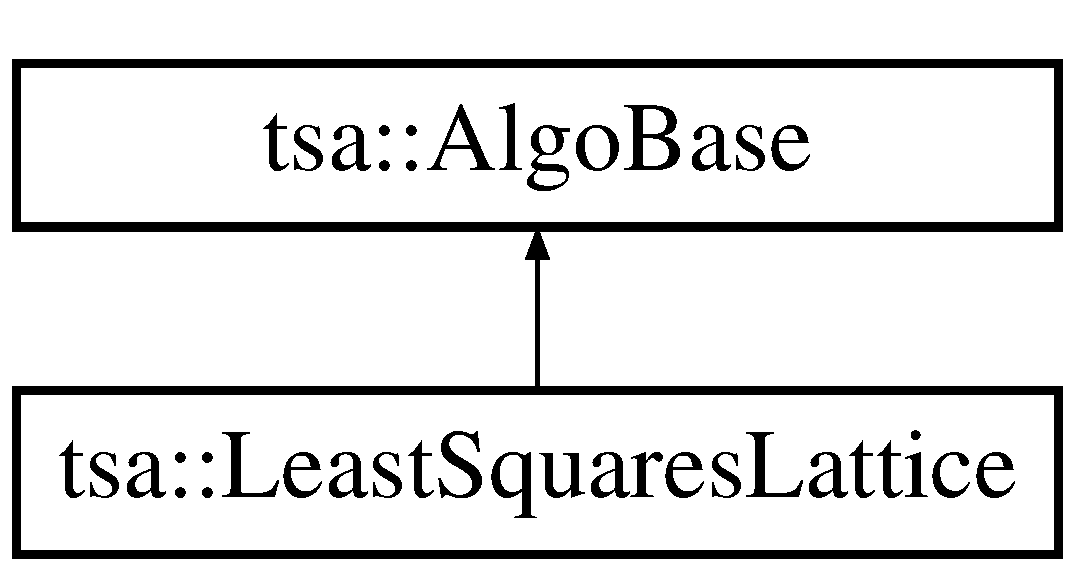
\includegraphics[height=2.000000cm]{classtsa_1_1_least_squares_lattice}
\end{center}
\end{figure}
\subsection*{Public Member Functions}
\begin{DoxyCompactItemize}
\item 
\hyperlink{classtsa_1_1_least_squares_lattice_a0fa6ec81a0438b15892c2dbc49932ea0}{Least\+Squares\+Lattice} (matrix\+\_\+row$<$ \hyperlink{namespacetsa_ad260cd21c1891c4ed391fe788569aba4}{Dmatrix} $>$ \&Learn\+Data, matrix\+\_\+row$<$ \hyperlink{namespacetsa_ad260cd21c1891c4ed391fe788569aba4}{Dmatrix} $>$ \&Whiten\+Data, unsigned int P, double lambda, unsigned int D)
\item 
virtual \hyperlink{classtsa_1_1_least_squares_lattice_a9a83bde1203dadf87892afcf25729081}{$\sim$\+Least\+Squares\+Lattice} ()
\item 
\hyperlink{classtsa_1_1_least_squares_lattice}{Least\+Squares\+Lattice} \& \hyperlink{classtsa_1_1_least_squares_lattice_a7037938b899e80b09bb34c053d1c7f41}{operator=} (const \hyperlink{classtsa_1_1_least_squares_lattice}{Least\+Squares\+Lattice} \&from)
\end{DoxyCompactItemize}
\begin{Indent}\textbf{ Operations}\par
\begin{DoxyCompactItemize}
\item 
void \hyperlink{classtsa_1_1_least_squares_lattice_a768ad13ebc89f33b627cc04e5131f7b4}{execute} (\hyperlink{namespacetsa_a8900fb03d849baf447a1a0efe2561fb2}{Dvector} \&Input, \hyperlink{namespacetsa_a8900fb03d849baf447a1a0efe2561fb2}{Dvector} \&Output)
\end{DoxyCompactItemize}
\end{Indent}
\subsection*{Private Attributes}
\begin{DoxyCompactItemize}
\item 
unsigned int \hyperlink{classtsa_1_1_least_squares_lattice_a714e35374ee38156cf0fa4816340a6df}{m\+Order}
\item 
unsigned int \hyperlink{classtsa_1_1_least_squares_lattice_a00bb9716623be7c8a035c9947023dcda}{m\+Lwsp}
\item 
double \hyperlink{classtsa_1_1_least_squares_lattice_a4b1315dc119c22efae15dd97168a5701}{m\+Lambda}
\item 
\hyperlink{namespacetsa_ad260cd21c1891c4ed391fe788569aba4}{Dmatrix} \hyperlink{classtsa_1_1_least_squares_lattice_a3170c018ba5b3dcfb91c9490e11e6199}{m\+Last}
\item 
unsigned \hyperlink{classtsa_1_1_least_squares_lattice_a40b578afe8b8e4523cc827337177412c}{m\+Direction}
\item 
unsigned int \hyperlink{classtsa_1_1_least_squares_lattice_a17c54dba21bbf5ae79d6687f554eceb9}{m\+Step}
\item 
\hyperlink{classtsa_1_1_l_s_l_learning}{L\+S\+L\+Learning} \hyperlink{classtsa_1_1_least_squares_lattice_a720cbccb82705799e96c4053cd1963af}{m\+L\+S\+Llearn}
\end{DoxyCompactItemize}


\subsection{Detailed Description}
Estimate the parameters for the Least Squares Lattice filter and implement the adaptive whitening. 

Definition at line 79 of file Least\+Squares\+Lattice.\+hpp.



\subsection{Constructor \& Destructor Documentation}
\mbox{\Hypertarget{classtsa_1_1_least_squares_lattice_a0fa6ec81a0438b15892c2dbc49932ea0}\label{classtsa_1_1_least_squares_lattice_a0fa6ec81a0438b15892c2dbc49932ea0}} 
\index{tsa\+::\+Least\+Squares\+Lattice@{tsa\+::\+Least\+Squares\+Lattice}!Least\+Squares\+Lattice@{Least\+Squares\+Lattice}}
\index{Least\+Squares\+Lattice@{Least\+Squares\+Lattice}!tsa\+::\+Least\+Squares\+Lattice@{tsa\+::\+Least\+Squares\+Lattice}}
\subsubsection{\texorpdfstring{Least\+Squares\+Lattice()}{LeastSquaresLattice()}}
{\footnotesize\ttfamily tsa\+::\+Least\+Squares\+Lattice\+::\+Least\+Squares\+Lattice (\begin{DoxyParamCaption}\item[{matrix\+\_\+row$<$ \hyperlink{namespacetsa_ad260cd21c1891c4ed391fe788569aba4}{Dmatrix} $>$ \&}]{Learn\+Data,  }\item[{matrix\+\_\+row$<$ \hyperlink{namespacetsa_ad260cd21c1891c4ed391fe788569aba4}{Dmatrix} $>$ \&}]{Whiten\+Data,  }\item[{unsigned int}]{P,  }\item[{double}]{lambda,  }\item[{unsigned int}]{D }\end{DoxyParamCaption})}

Constructor 

Definition at line 19 of file Least\+Squares\+Lattice.\+cpp.

\mbox{\Hypertarget{classtsa_1_1_least_squares_lattice_a9a83bde1203dadf87892afcf25729081}\label{classtsa_1_1_least_squares_lattice_a9a83bde1203dadf87892afcf25729081}} 
\index{tsa\+::\+Least\+Squares\+Lattice@{tsa\+::\+Least\+Squares\+Lattice}!````~Least\+Squares\+Lattice@{$\sim$\+Least\+Squares\+Lattice}}
\index{````~Least\+Squares\+Lattice@{$\sim$\+Least\+Squares\+Lattice}!tsa\+::\+Least\+Squares\+Lattice@{tsa\+::\+Least\+Squares\+Lattice}}
\subsubsection{\texorpdfstring{$\sim$\+Least\+Squares\+Lattice()}{~LeastSquaresLattice()}}
{\footnotesize\ttfamily tsa\+::\+Least\+Squares\+Lattice\+::$\sim$\+Least\+Squares\+Lattice (\begin{DoxyParamCaption}{ }\end{DoxyParamCaption})\hspace{0.3cm}{\ttfamily [virtual]}}

Destructor 

Definition at line 38 of file Least\+Squares\+Lattice.\+cpp.



\subsection{Member Function Documentation}
\mbox{\Hypertarget{classtsa_1_1_least_squares_lattice_a768ad13ebc89f33b627cc04e5131f7b4}\label{classtsa_1_1_least_squares_lattice_a768ad13ebc89f33b627cc04e5131f7b4}} 
\index{tsa\+::\+Least\+Squares\+Lattice@{tsa\+::\+Least\+Squares\+Lattice}!execute@{execute}}
\index{execute@{execute}!tsa\+::\+Least\+Squares\+Lattice@{tsa\+::\+Least\+Squares\+Lattice}}
\subsubsection{\texorpdfstring{execute()}{execute()}}
{\footnotesize\ttfamily void tsa\+::\+Least\+Squares\+Lattice\+::execute (\begin{DoxyParamCaption}\item[{\hyperlink{namespacetsa_a8900fb03d849baf447a1a0efe2561fb2}{Dvector} \&}]{Input,  }\item[{\hyperlink{namespacetsa_a8900fb03d849baf447a1a0efe2561fb2}{Dvector} \&}]{Output }\end{DoxyParamCaption})}


\begin{DoxyParams}{Parameters}
{\em Input} & Input data \\
\hline
{\em Output} & Whitened Data \\
\hline
\end{DoxyParams}
\mbox{\Hypertarget{classtsa_1_1_least_squares_lattice_a7037938b899e80b09bb34c053d1c7f41}\label{classtsa_1_1_least_squares_lattice_a7037938b899e80b09bb34c053d1c7f41}} 
\index{tsa\+::\+Least\+Squares\+Lattice@{tsa\+::\+Least\+Squares\+Lattice}!operator=@{operator=}}
\index{operator=@{operator=}!tsa\+::\+Least\+Squares\+Lattice@{tsa\+::\+Least\+Squares\+Lattice}}
\subsubsection{\texorpdfstring{operator=()}{operator=()}}
{\footnotesize\ttfamily \hyperlink{classtsa_1_1_least_squares_lattice}{Least\+Squares\+Lattice} \& tsa\+::\+Least\+Squares\+Lattice\+::operator= (\begin{DoxyParamCaption}\item[{const \hyperlink{classtsa_1_1_least_squares_lattice}{Least\+Squares\+Lattice} \&}]{from }\end{DoxyParamCaption})}

Assignement operator


\begin{DoxyParams}{Parameters}
{\em from} & The instance to be assigned from\\
\hline
\end{DoxyParams}
\begin{DoxyReturn}{Returns}
a reference to a new object 
\end{DoxyReturn}


Definition at line 49 of file Least\+Squares\+Lattice.\+cpp.



\subsection{Member Data Documentation}
\mbox{\Hypertarget{classtsa_1_1_least_squares_lattice_a40b578afe8b8e4523cc827337177412c}\label{classtsa_1_1_least_squares_lattice_a40b578afe8b8e4523cc827337177412c}} 
\index{tsa\+::\+Least\+Squares\+Lattice@{tsa\+::\+Least\+Squares\+Lattice}!m\+Direction@{m\+Direction}}
\index{m\+Direction@{m\+Direction}!tsa\+::\+Least\+Squares\+Lattice@{tsa\+::\+Least\+Squares\+Lattice}}
\subsubsection{\texorpdfstring{m\+Direction}{mDirection}}
{\footnotesize\ttfamily unsigned tsa\+::\+Least\+Squares\+Lattice\+::m\+Direction\hspace{0.3cm}{\ttfamily [private]}}



Definition at line 139 of file Least\+Squares\+Lattice.\+hpp.

\mbox{\Hypertarget{classtsa_1_1_least_squares_lattice_a4b1315dc119c22efae15dd97168a5701}\label{classtsa_1_1_least_squares_lattice_a4b1315dc119c22efae15dd97168a5701}} 
\index{tsa\+::\+Least\+Squares\+Lattice@{tsa\+::\+Least\+Squares\+Lattice}!m\+Lambda@{m\+Lambda}}
\index{m\+Lambda@{m\+Lambda}!tsa\+::\+Least\+Squares\+Lattice@{tsa\+::\+Least\+Squares\+Lattice}}
\subsubsection{\texorpdfstring{m\+Lambda}{mLambda}}
{\footnotesize\ttfamily double tsa\+::\+Least\+Squares\+Lattice\+::m\+Lambda\hspace{0.3cm}{\ttfamily [private]}}



Definition at line 137 of file Least\+Squares\+Lattice.\+hpp.

\mbox{\Hypertarget{classtsa_1_1_least_squares_lattice_a3170c018ba5b3dcfb91c9490e11e6199}\label{classtsa_1_1_least_squares_lattice_a3170c018ba5b3dcfb91c9490e11e6199}} 
\index{tsa\+::\+Least\+Squares\+Lattice@{tsa\+::\+Least\+Squares\+Lattice}!m\+Last@{m\+Last}}
\index{m\+Last@{m\+Last}!tsa\+::\+Least\+Squares\+Lattice@{tsa\+::\+Least\+Squares\+Lattice}}
\subsubsection{\texorpdfstring{m\+Last}{mLast}}
{\footnotesize\ttfamily \hyperlink{namespacetsa_ad260cd21c1891c4ed391fe788569aba4}{Dmatrix} tsa\+::\+Least\+Squares\+Lattice\+::m\+Last\hspace{0.3cm}{\ttfamily [private]}}



Definition at line 138 of file Least\+Squares\+Lattice.\+hpp.

\mbox{\Hypertarget{classtsa_1_1_least_squares_lattice_a720cbccb82705799e96c4053cd1963af}\label{classtsa_1_1_least_squares_lattice_a720cbccb82705799e96c4053cd1963af}} 
\index{tsa\+::\+Least\+Squares\+Lattice@{tsa\+::\+Least\+Squares\+Lattice}!m\+L\+S\+Llearn@{m\+L\+S\+Llearn}}
\index{m\+L\+S\+Llearn@{m\+L\+S\+Llearn}!tsa\+::\+Least\+Squares\+Lattice@{tsa\+::\+Least\+Squares\+Lattice}}
\subsubsection{\texorpdfstring{m\+L\+S\+Llearn}{mLSLlearn}}
{\footnotesize\ttfamily \hyperlink{classtsa_1_1_l_s_l_learning}{L\+S\+L\+Learning} tsa\+::\+Least\+Squares\+Lattice\+::m\+L\+S\+Llearn\hspace{0.3cm}{\ttfamily [private]}}



Definition at line 141 of file Least\+Squares\+Lattice.\+hpp.

\mbox{\Hypertarget{classtsa_1_1_least_squares_lattice_a00bb9716623be7c8a035c9947023dcda}\label{classtsa_1_1_least_squares_lattice_a00bb9716623be7c8a035c9947023dcda}} 
\index{tsa\+::\+Least\+Squares\+Lattice@{tsa\+::\+Least\+Squares\+Lattice}!m\+Lwsp@{m\+Lwsp}}
\index{m\+Lwsp@{m\+Lwsp}!tsa\+::\+Least\+Squares\+Lattice@{tsa\+::\+Least\+Squares\+Lattice}}
\subsubsection{\texorpdfstring{m\+Lwsp}{mLwsp}}
{\footnotesize\ttfamily unsigned int tsa\+::\+Least\+Squares\+Lattice\+::m\+Lwsp\hspace{0.3cm}{\ttfamily [private]}}



Definition at line 136 of file Least\+Squares\+Lattice.\+hpp.

\mbox{\Hypertarget{classtsa_1_1_least_squares_lattice_a714e35374ee38156cf0fa4816340a6df}\label{classtsa_1_1_least_squares_lattice_a714e35374ee38156cf0fa4816340a6df}} 
\index{tsa\+::\+Least\+Squares\+Lattice@{tsa\+::\+Least\+Squares\+Lattice}!m\+Order@{m\+Order}}
\index{m\+Order@{m\+Order}!tsa\+::\+Least\+Squares\+Lattice@{tsa\+::\+Least\+Squares\+Lattice}}
\subsubsection{\texorpdfstring{m\+Order}{mOrder}}
{\footnotesize\ttfamily unsigned int tsa\+::\+Least\+Squares\+Lattice\+::m\+Order\hspace{0.3cm}{\ttfamily [private]}}



Definition at line 135 of file Least\+Squares\+Lattice.\+hpp.

\mbox{\Hypertarget{classtsa_1_1_least_squares_lattice_a17c54dba21bbf5ae79d6687f554eceb9}\label{classtsa_1_1_least_squares_lattice_a17c54dba21bbf5ae79d6687f554eceb9}} 
\index{tsa\+::\+Least\+Squares\+Lattice@{tsa\+::\+Least\+Squares\+Lattice}!m\+Step@{m\+Step}}
\index{m\+Step@{m\+Step}!tsa\+::\+Least\+Squares\+Lattice@{tsa\+::\+Least\+Squares\+Lattice}}
\subsubsection{\texorpdfstring{m\+Step}{mStep}}
{\footnotesize\ttfamily unsigned int tsa\+::\+Least\+Squares\+Lattice\+::m\+Step\hspace{0.3cm}{\ttfamily [private]}}



Definition at line 140 of file Least\+Squares\+Lattice.\+hpp.



The documentation for this class was generated from the following files\+:\begin{DoxyCompactItemize}
\item 
/home/filip/\+Ph\+D/\+W\+D\+F\+Pipe\+\_\+test/p4\+T\+S\+A/include/\hyperlink{_least_squares_lattice_8hpp}{Least\+Squares\+Lattice.\+hpp}\item 
/home/filip/\+Ph\+D/\+W\+D\+F\+Pipe\+\_\+test/p4\+T\+S\+A/src/\hyperlink{_least_squares_lattice_8cpp}{Least\+Squares\+Lattice.\+cpp}\end{DoxyCompactItemize}

\hypertarget{classtsa_1_1_lower_triangular}{}\section{tsa\+:\+:Lower\+Triangular Class Reference}
\label{classtsa_1_1_lower_triangular}\index{tsa\+::\+Lower\+Triangular@{tsa\+::\+Lower\+Triangular}}


{\ttfamily \#include $<$tsa\+Utility\+Functions.\+hpp$>$}

\subsection*{Static Public Member Functions}
\begin{DoxyCompactItemize}
\item 
static unsigned int \hyperlink{classtsa_1_1_lower_triangular_a968298d0e21e8eff3959fe9eb69eee8a}{Map} (unsigned int i, unsigned int j, unsigned int)
\item 
static unsigned int \hyperlink{classtsa_1_1_lower_triangular_a553ac56eb5320ef223c61951290429d0}{Size} (unsigned int dim)
\item 
static unsigned int \hyperlink{classtsa_1_1_lower_triangular_ae0be1ed16dc6f469852699898aa16df3}{Dimension} (unsigned int sz)
\end{DoxyCompactItemize}


\subsection{Detailed Description}


Definition at line 211 of file tsa\+Utility\+Functions.\+hpp.



\subsection{Member Function Documentation}
\mbox{\Hypertarget{classtsa_1_1_lower_triangular_ae0be1ed16dc6f469852699898aa16df3}\label{classtsa_1_1_lower_triangular_ae0be1ed16dc6f469852699898aa16df3}} 
\index{tsa\+::\+Lower\+Triangular@{tsa\+::\+Lower\+Triangular}!Dimension@{Dimension}}
\index{Dimension@{Dimension}!tsa\+::\+Lower\+Triangular@{tsa\+::\+Lower\+Triangular}}
\subsubsection{\texorpdfstring{Dimension()}{Dimension()}}
{\footnotesize\ttfamily static unsigned int tsa\+::\+Lower\+Triangular\+::\+Dimension (\begin{DoxyParamCaption}\item[{unsigned int}]{sz }\end{DoxyParamCaption})\hspace{0.3cm}{\ttfamily [inline]}, {\ttfamily [static]}}



Definition at line 222 of file tsa\+Utility\+Functions.\+hpp.

\mbox{\Hypertarget{classtsa_1_1_lower_triangular_a968298d0e21e8eff3959fe9eb69eee8a}\label{classtsa_1_1_lower_triangular_a968298d0e21e8eff3959fe9eb69eee8a}} 
\index{tsa\+::\+Lower\+Triangular@{tsa\+::\+Lower\+Triangular}!Map@{Map}}
\index{Map@{Map}!tsa\+::\+Lower\+Triangular@{tsa\+::\+Lower\+Triangular}}
\subsubsection{\texorpdfstring{Map()}{Map()}}
{\footnotesize\ttfamily static unsigned int tsa\+::\+Lower\+Triangular\+::\+Map (\begin{DoxyParamCaption}\item[{unsigned int}]{i,  }\item[{unsigned int}]{j,  }\item[{unsigned}]{int }\end{DoxyParamCaption})\hspace{0.3cm}{\ttfamily [inline]}, {\ttfamily [static]}}



Definition at line 214 of file tsa\+Utility\+Functions.\+hpp.

\mbox{\Hypertarget{classtsa_1_1_lower_triangular_a553ac56eb5320ef223c61951290429d0}\label{classtsa_1_1_lower_triangular_a553ac56eb5320ef223c61951290429d0}} 
\index{tsa\+::\+Lower\+Triangular@{tsa\+::\+Lower\+Triangular}!Size@{Size}}
\index{Size@{Size}!tsa\+::\+Lower\+Triangular@{tsa\+::\+Lower\+Triangular}}
\subsubsection{\texorpdfstring{Size()}{Size()}}
{\footnotesize\ttfamily static unsigned int tsa\+::\+Lower\+Triangular\+::\+Size (\begin{DoxyParamCaption}\item[{unsigned int}]{dim }\end{DoxyParamCaption})\hspace{0.3cm}{\ttfamily [inline]}, {\ttfamily [static]}}



Definition at line 218 of file tsa\+Utility\+Functions.\+hpp.



The documentation for this class was generated from the following file\+:\begin{DoxyCompactItemize}
\item 
/home/filip/\+Ph\+D/\+W\+D\+F\+Pipe\+\_\+test/p4\+T\+S\+A/include/\hyperlink{tsa_utility_functions_8hpp}{tsa\+Utility\+Functions.\+hpp}\end{DoxyCompactItemize}

\hypertarget{classtsa_1_1_l_s_lfilter}{}\section{tsa\+:\+:L\+S\+Lfilter Class Reference}
\label{classtsa_1_1_l_s_lfilter}\index{tsa\+::\+L\+S\+Lfilter@{tsa\+::\+L\+S\+Lfilter}}


Algorithm for the filter phase of the Adaptive Least Squares Lattice.  




{\ttfamily \#include $<$L\+S\+Lfilter.\+hpp$>$}

Inheritance diagram for tsa\+:\+:L\+S\+Lfilter\+:\begin{figure}[H]
\begin{center}
\leavevmode
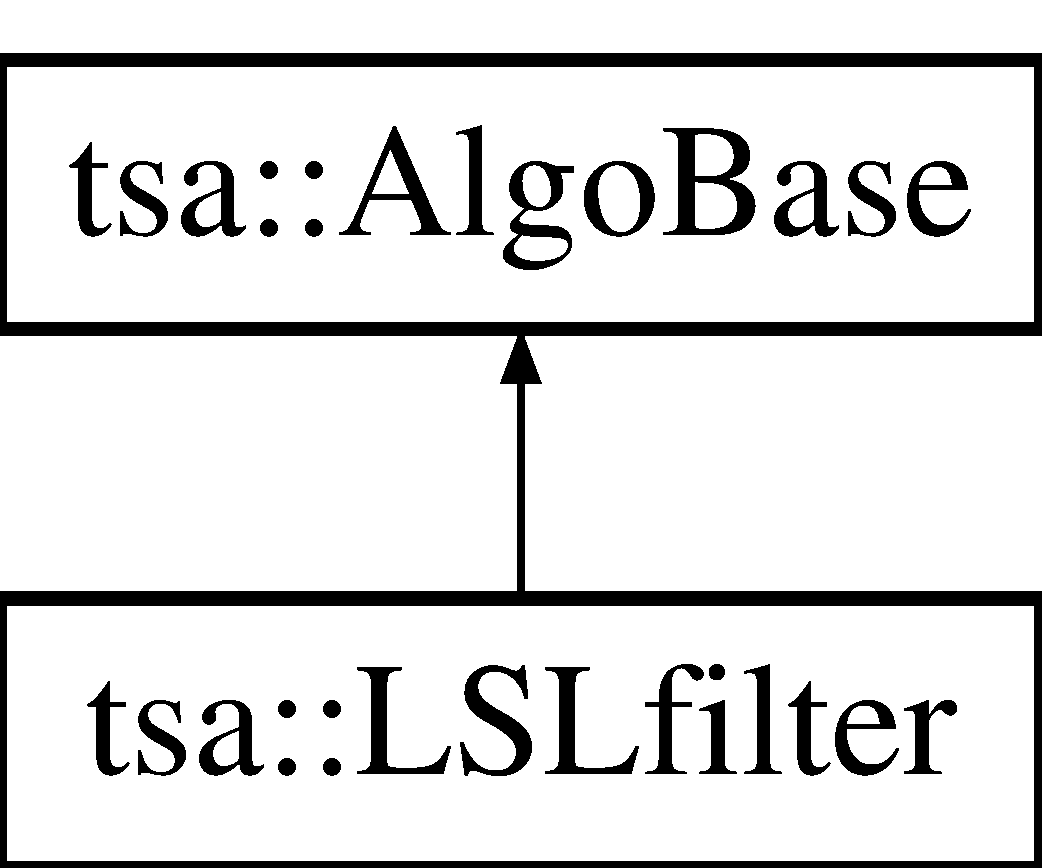
\includegraphics[height=2.000000cm]{classtsa_1_1_l_s_lfilter}
\end{center}
\end{figure}
\subsection*{Public Member Functions}
\begin{DoxyCompactItemize}
\item 
\hyperlink{classtsa_1_1_l_s_lfilter_a7f49b52bb9e1b935f957e04166bf7c8c}{L\+S\+Lfilter} (\hyperlink{classtsa_1_1_l_s_l_learning}{L\+S\+L\+Learning} \&L\+SL, double lambda=1.\+0, unsigned int size=1, bool Norm=false)
\item 
\hyperlink{classtsa_1_1_l_s_lfilter_addf16b957be6c848ad1c59ee7cb4dd4e}{$\sim$\+L\+S\+Lfilter} ()
\item 
void \hyperlink{classtsa_1_1_l_s_lfilter_a737d772a9b51efdd71a01178ec83597f}{Load} (const char $\ast$filename, const char $\ast$fmt=\char`\"{}txt\char`\"{})
\item 
void \hyperlink{classtsa_1_1_l_s_lfilter_ae8aa6f5275313f49e88bf4f6361092f9}{Save} (const char $\ast$filename, const char $\ast$fmt=\char`\"{}txt\char`\"{})
\item 
void \hyperlink{classtsa_1_1_l_s_lfilter_a1adaa3058f09e50b73a88520844d2b90}{xml\+\_\+serialize} (\hyperlink{classeternity_1_1xml__archive}{eternity\+::xml\+\_\+archive} \&xml, const char $\ast$p)
\item 
int \hyperlink{classtsa_1_1_l_s_lfilter_a236a35327bce862b6c4f8a9245af7b9c}{Get\+Data\+Needed} ()
\end{DoxyCompactItemize}
\begin{Indent}\textbf{ Operations}\par
\begin{DoxyCompactItemize}
\item 
void \hyperlink{classtsa_1_1_l_s_lfilter_a4308a18bd0ecc82242c4df0529c1f573}{operator$<$$<$} (\hyperlink{namespacetsa_ac599574bcc094eda25613724b8f3ca9e}{Seq\+View\+Double} \&Data)
\begin{DoxyCompactList}\small\item\em to be used only when data are contiguos (offline analysis) \end{DoxyCompactList}\item 
void \hyperlink{classtsa_1_1_l_s_lfilter_a8b0ecd9fa51d407daf718ac91776ebed}{operator$>$$>$} (\hyperlink{namespacetsa_ac599574bcc094eda25613724b8f3ca9e}{Seq\+View\+Double} \&outdata)
\item 
void \hyperlink{classtsa_1_1_l_s_lfilter_a7a6f64f53279b310e23cb034ab1d9a99}{operator()} (\hyperlink{namespacetsa_ac599574bcc094eda25613724b8f3ca9e}{Seq\+View\+Double} \&Data, \hyperlink{namespacetsa_ac599574bcc094eda25613724b8f3ca9e}{Seq\+View\+Double} \&outdata)
\begin{DoxyCompactList}\small\item\em for online process \end{DoxyCompactList}\end{DoxyCompactItemize}
\end{Indent}
\begin{Indent}\textbf{ Getters}\par
\begin{DoxyCompactItemize}
\item 
void \hyperlink{classtsa_1_1_l_s_lfilter_ad577b856b131f49de4e29eb2406560e9}{Get\+Data} (\hyperlink{namespacetsa_ad260cd21c1891c4ed391fe788569aba4}{Dmatrix} \&D\+W\+Output)
\item 
\hyperlink{namespacetsa_ad260cd21c1891c4ed391fe788569aba4}{Dmatrix} $\ast$ \hyperlink{classtsa_1_1_l_s_lfilter_a4b15685dc591ec522e2a34edcf87082b}{Get\+Whitened\+Matrix} ()
\item 
unsigned int \hyperlink{classtsa_1_1_l_s_lfilter_af7e46359752bd2839f4ed510ef625ce5}{Get\+Order} ()
\item 
double \hyperlink{classtsa_1_1_l_s_lfilter_a3a04a948854ddde91e3aa4bd8a5bf0eb}{Get\+Parcor\+Forward} (unsigned int j)
\item 
double \hyperlink{classtsa_1_1_l_s_lfilter_a21f41a8a1cbb800d0a1d4c3e474cc51e}{Get\+Parcor\+Backward} (unsigned int j)
\item 
double \hyperlink{classtsa_1_1_l_s_lfilter_a94d29deb2900d3be889b1288730112df}{Get\+Epf} (unsigned int j)
\item 
double \hyperlink{classtsa_1_1_l_s_lfilter_aad172e3d7c8743ea64b0dd32d9017bbd}{Get\+Error\+Forward} (unsigned int j)
\item 
double \hyperlink{classtsa_1_1_l_s_lfilter_ad9c27bb102a3cd25ceda75ab5bed4a7a}{Get\+Error\+Backward} (unsigned int j)
\item 
double \hyperlink{classtsa_1_1_l_s_lfilter_a06bbde7bf7ba9deed211b3a05ba82890}{Get\+Sigma} (unsigned int j)
\end{DoxyCompactItemize}
\end{Indent}
\begin{Indent}\textbf{ Setters}\par
\begin{DoxyCompactItemize}
\item 
void \hyperlink{classtsa_1_1_l_s_lfilter_ab01da31972cf54c49a28920c8235e8c9}{Set\+Data} (\hyperlink{namespacetsa_ad260cd21c1891c4ed391fe788569aba4}{Dmatrix} \&Data, double scale)
\end{DoxyCompactItemize}
\end{Indent}
\subsection*{Private Attributes}
\begin{DoxyCompactItemize}
\item 
\hyperlink{classtsa_1_1_fifo_buffer}{Fifo\+Buffer} \hyperlink{classtsa_1_1_l_s_lfilter_a95e5134738dd70857cf6c7ac52b11639}{m\+Buffer}
\item 
unsigned int \hyperlink{classtsa_1_1_l_s_lfilter_a015aba5b8378277ee5cda011ba6b4fe1}{m\+Win\+Size}
\item 
unsigned int \hyperlink{classtsa_1_1_l_s_lfilter_aa25b337e262a868101f68d8437f162c1}{m\+Order}
\item 
double \hyperlink{classtsa_1_1_l_s_lfilter_aeae300f77e90ba968cc9c5c0eea38a96}{m\+Lambda}
\item 
\hyperlink{namespacetsa_a8900fb03d849baf447a1a0efe2561fb2}{Dvector} \hyperlink{classtsa_1_1_l_s_lfilter_aa620a0738568ad5360806ad189aa70c2}{m\+Sigma}
\item 
bool \hyperlink{classtsa_1_1_l_s_lfilter_a68dda41fd3d7be90171213425541ea2a}{m\+Norm}
\item 
double \hyperlink{classtsa_1_1_l_s_lfilter_a9898a4187911d742deb802e51ec1883f}{m\+Sigma0}
\item 
double \hyperlink{classtsa_1_1_l_s_lfilter_a6e679e1858ec5cab2c2ab00d9ad17a4b}{m\+Start\+Time}
\item 
double \hyperlink{classtsa_1_1_l_s_lfilter_a7d7cc212e5c6a963560a6f18eff72497}{m\+Sampling}
\item 
bool \hyperlink{classtsa_1_1_l_s_lfilter_a23612cc3cfdb9a0dfb38743f54e4d076}{m\+First\+Call}
\item 
\hyperlink{namespacetsa_ad260cd21c1891c4ed391fe788569aba4}{Dmatrix} \hyperlink{classtsa_1_1_l_s_lfilter_a980bad9cc152c400df6f4e1e8c25c111}{m\+EF}
\item 
\hyperlink{namespacetsa_ad260cd21c1891c4ed391fe788569aba4}{Dmatrix} \hyperlink{classtsa_1_1_l_s_lfilter_a24ad0a2f6a2b79b01b1e99ef9c663d1e}{m\+EB}
\item 
\hyperlink{namespacetsa_ad260cd21c1891c4ed391fe788569aba4}{Dmatrix} \hyperlink{classtsa_1_1_l_s_lfilter_a571c1d1b411aad2417ce23579a8da9ac}{m\+Epf}
\item 
\hyperlink{namespacetsa_ad260cd21c1891c4ed391fe788569aba4}{Dmatrix} \hyperlink{classtsa_1_1_l_s_lfilter_a067ccd52ecffc15945fdcb73fa515244}{m\+Epb}
\item 
\hyperlink{namespacetsa_a8900fb03d849baf447a1a0efe2561fb2}{Dvector} \hyperlink{classtsa_1_1_l_s_lfilter_a83a3095a513fda5efd6b75aaa77495df}{m\+Kf}
\item 
\hyperlink{namespacetsa_a8900fb03d849baf447a1a0efe2561fb2}{Dvector} \hyperlink{classtsa_1_1_l_s_lfilter_ae3b9ac48debc547e1aa69ae0ade36408}{m\+Kb}
\item 
\hyperlink{namespacetsa_a8900fb03d849baf447a1a0efe2561fb2}{Dvector} \hyperlink{classtsa_1_1_l_s_lfilter_a0a2ad9e25528879045483500ff6401b0}{mG}
\item 
unsigned int \hyperlink{classtsa_1_1_l_s_lfilter_a490187ff893b2ff71a5f36f9b4efe7f3}{m\+F0}
\end{DoxyCompactItemize}


\subsection{Detailed Description}
Algorithm for the filter phase of the Adaptive Least Squares Lattice. 

Definition at line 76 of file L\+S\+Lfilter.\+hpp.



\subsection{Constructor \& Destructor Documentation}
\mbox{\Hypertarget{classtsa_1_1_l_s_lfilter_a7f49b52bb9e1b935f957e04166bf7c8c}\label{classtsa_1_1_l_s_lfilter_a7f49b52bb9e1b935f957e04166bf7c8c}} 
\index{tsa\+::\+L\+S\+Lfilter@{tsa\+::\+L\+S\+Lfilter}!L\+S\+Lfilter@{L\+S\+Lfilter}}
\index{L\+S\+Lfilter@{L\+S\+Lfilter}!tsa\+::\+L\+S\+Lfilter@{tsa\+::\+L\+S\+Lfilter}}
\subsubsection{\texorpdfstring{L\+S\+Lfilter()}{LSLfilter()}}
{\footnotesize\ttfamily tsa\+::\+L\+S\+Lfilter\+::\+L\+S\+Lfilter (\begin{DoxyParamCaption}\item[{\hyperlink{classtsa_1_1_l_s_l_learning}{L\+S\+L\+Learning} \&}]{L\+SL,  }\item[{double}]{lambda = {\ttfamily 1.0},  }\item[{unsigned int}]{size = {\ttfamily 1},  }\item[{bool}]{Norm = {\ttfamily false} }\end{DoxyParamCaption})}

Constructor


\begin{DoxyParams}{Parameters}
{\em Order} & Order of the filter \\
\hline
{\em sigma} & guessed value for the initial sigma \\
\hline
{\em Lwsp} & Lenght of workspace \\
\hline
{\em lambda} & forgetting factor \\
\hline
\end{DoxyParams}


Definition at line 20 of file L\+S\+Lfilter.\+cpp.

\mbox{\Hypertarget{classtsa_1_1_l_s_lfilter_addf16b957be6c848ad1c59ee7cb4dd4e}\label{classtsa_1_1_l_s_lfilter_addf16b957be6c848ad1c59ee7cb4dd4e}} 
\index{tsa\+::\+L\+S\+Lfilter@{tsa\+::\+L\+S\+Lfilter}!````~L\+S\+Lfilter@{$\sim$\+L\+S\+Lfilter}}
\index{````~L\+S\+Lfilter@{$\sim$\+L\+S\+Lfilter}!tsa\+::\+L\+S\+Lfilter@{tsa\+::\+L\+S\+Lfilter}}
\subsubsection{\texorpdfstring{$\sim$\+L\+S\+Lfilter()}{~LSLfilter()}}
{\footnotesize\ttfamily tsa\+::\+L\+S\+Lfilter\+::$\sim$\+L\+S\+Lfilter (\begin{DoxyParamCaption}{ }\end{DoxyParamCaption})}

Destructor 

Definition at line 49 of file L\+S\+Lfilter.\+cpp.



\subsection{Member Function Documentation}
\mbox{\Hypertarget{classtsa_1_1_l_s_lfilter_ad577b856b131f49de4e29eb2406560e9}\label{classtsa_1_1_l_s_lfilter_ad577b856b131f49de4e29eb2406560e9}} 
\index{tsa\+::\+L\+S\+Lfilter@{tsa\+::\+L\+S\+Lfilter}!Get\+Data@{Get\+Data}}
\index{Get\+Data@{Get\+Data}!tsa\+::\+L\+S\+Lfilter@{tsa\+::\+L\+S\+Lfilter}}
\subsubsection{\texorpdfstring{Get\+Data()}{GetData()}}
{\footnotesize\ttfamily void tsa\+::\+L\+S\+Lfilter\+::\+Get\+Data (\begin{DoxyParamCaption}\item[{\hyperlink{namespacetsa_ad260cd21c1891c4ed391fe788569aba4}{Dmatrix} \&}]{D\+W\+Output }\end{DoxyParamCaption})}



Definition at line 63 of file L\+S\+Lfilter.\+cpp.

\mbox{\Hypertarget{classtsa_1_1_l_s_lfilter_a236a35327bce862b6c4f8a9245af7b9c}\label{classtsa_1_1_l_s_lfilter_a236a35327bce862b6c4f8a9245af7b9c}} 
\index{tsa\+::\+L\+S\+Lfilter@{tsa\+::\+L\+S\+Lfilter}!Get\+Data\+Needed@{Get\+Data\+Needed}}
\index{Get\+Data\+Needed@{Get\+Data\+Needed}!tsa\+::\+L\+S\+Lfilter@{tsa\+::\+L\+S\+Lfilter}}
\subsubsection{\texorpdfstring{Get\+Data\+Needed()}{GetDataNeeded()}}
{\footnotesize\ttfamily int tsa\+::\+L\+S\+Lfilter\+::\+Get\+Data\+Needed (\begin{DoxyParamCaption}{ }\end{DoxyParamCaption})}

Get the number of data needed in order to be able to call Get\+Data successfully. If the returned value is less or equal than zero no data are needed.

\begin{DoxyReturn}{Returns}
the needed data 
\end{DoxyReturn}


Definition at line 57 of file L\+S\+Lfilter.\+cpp.

\mbox{\Hypertarget{classtsa_1_1_l_s_lfilter_a94d29deb2900d3be889b1288730112df}\label{classtsa_1_1_l_s_lfilter_a94d29deb2900d3be889b1288730112df}} 
\index{tsa\+::\+L\+S\+Lfilter@{tsa\+::\+L\+S\+Lfilter}!Get\+Epf@{Get\+Epf}}
\index{Get\+Epf@{Get\+Epf}!tsa\+::\+L\+S\+Lfilter@{tsa\+::\+L\+S\+Lfilter}}
\subsubsection{\texorpdfstring{Get\+Epf()}{GetEpf()}}
{\footnotesize\ttfamily double tsa\+::\+L\+S\+Lfilter\+::\+Get\+Epf (\begin{DoxyParamCaption}\item[{unsigned int}]{j }\end{DoxyParamCaption})\hspace{0.3cm}{\ttfamily [inline]}}



Definition at line 326 of file L\+S\+Lfilter.\+hpp.

\mbox{\Hypertarget{classtsa_1_1_l_s_lfilter_ad9c27bb102a3cd25ceda75ab5bed4a7a}\label{classtsa_1_1_l_s_lfilter_ad9c27bb102a3cd25ceda75ab5bed4a7a}} 
\index{tsa\+::\+L\+S\+Lfilter@{tsa\+::\+L\+S\+Lfilter}!Get\+Error\+Backward@{Get\+Error\+Backward}}
\index{Get\+Error\+Backward@{Get\+Error\+Backward}!tsa\+::\+L\+S\+Lfilter@{tsa\+::\+L\+S\+Lfilter}}
\subsubsection{\texorpdfstring{Get\+Error\+Backward()}{GetErrorBackward()}}
{\footnotesize\ttfamily double tsa\+::\+L\+S\+Lfilter\+::\+Get\+Error\+Backward (\begin{DoxyParamCaption}\item[{unsigned int}]{j }\end{DoxyParamCaption})\hspace{0.3cm}{\ttfamily [inline]}}



Definition at line 336 of file L\+S\+Lfilter.\+hpp.

\mbox{\Hypertarget{classtsa_1_1_l_s_lfilter_aad172e3d7c8743ea64b0dd32d9017bbd}\label{classtsa_1_1_l_s_lfilter_aad172e3d7c8743ea64b0dd32d9017bbd}} 
\index{tsa\+::\+L\+S\+Lfilter@{tsa\+::\+L\+S\+Lfilter}!Get\+Error\+Forward@{Get\+Error\+Forward}}
\index{Get\+Error\+Forward@{Get\+Error\+Forward}!tsa\+::\+L\+S\+Lfilter@{tsa\+::\+L\+S\+Lfilter}}
\subsubsection{\texorpdfstring{Get\+Error\+Forward()}{GetErrorForward()}}
{\footnotesize\ttfamily double tsa\+::\+L\+S\+Lfilter\+::\+Get\+Error\+Forward (\begin{DoxyParamCaption}\item[{unsigned int}]{j }\end{DoxyParamCaption})\hspace{0.3cm}{\ttfamily [inline]}}



Definition at line 330 of file L\+S\+Lfilter.\+hpp.

\mbox{\Hypertarget{classtsa_1_1_l_s_lfilter_af7e46359752bd2839f4ed510ef625ce5}\label{classtsa_1_1_l_s_lfilter_af7e46359752bd2839f4ed510ef625ce5}} 
\index{tsa\+::\+L\+S\+Lfilter@{tsa\+::\+L\+S\+Lfilter}!Get\+Order@{Get\+Order}}
\index{Get\+Order@{Get\+Order}!tsa\+::\+L\+S\+Lfilter@{tsa\+::\+L\+S\+Lfilter}}
\subsubsection{\texorpdfstring{Get\+Order()}{GetOrder()}}
{\footnotesize\ttfamily unsigned int tsa\+::\+L\+S\+Lfilter\+::\+Get\+Order (\begin{DoxyParamCaption}{ }\end{DoxyParamCaption})\hspace{0.3cm}{\ttfamily [inline]}}



Definition at line 311 of file L\+S\+Lfilter.\+hpp.

\mbox{\Hypertarget{classtsa_1_1_l_s_lfilter_a21f41a8a1cbb800d0a1d4c3e474cc51e}\label{classtsa_1_1_l_s_lfilter_a21f41a8a1cbb800d0a1d4c3e474cc51e}} 
\index{tsa\+::\+L\+S\+Lfilter@{tsa\+::\+L\+S\+Lfilter}!Get\+Parcor\+Backward@{Get\+Parcor\+Backward}}
\index{Get\+Parcor\+Backward@{Get\+Parcor\+Backward}!tsa\+::\+L\+S\+Lfilter@{tsa\+::\+L\+S\+Lfilter}}
\subsubsection{\texorpdfstring{Get\+Parcor\+Backward()}{GetParcorBackward()}}
{\footnotesize\ttfamily double tsa\+::\+L\+S\+Lfilter\+::\+Get\+Parcor\+Backward (\begin{DoxyParamCaption}\item[{unsigned int}]{j }\end{DoxyParamCaption})\hspace{0.3cm}{\ttfamily [inline]}}



Definition at line 322 of file L\+S\+Lfilter.\+hpp.

\mbox{\Hypertarget{classtsa_1_1_l_s_lfilter_a3a04a948854ddde91e3aa4bd8a5bf0eb}\label{classtsa_1_1_l_s_lfilter_a3a04a948854ddde91e3aa4bd8a5bf0eb}} 
\index{tsa\+::\+L\+S\+Lfilter@{tsa\+::\+L\+S\+Lfilter}!Get\+Parcor\+Forward@{Get\+Parcor\+Forward}}
\index{Get\+Parcor\+Forward@{Get\+Parcor\+Forward}!tsa\+::\+L\+S\+Lfilter@{tsa\+::\+L\+S\+Lfilter}}
\subsubsection{\texorpdfstring{Get\+Parcor\+Forward()}{GetParcorForward()}}
{\footnotesize\ttfamily double tsa\+::\+L\+S\+Lfilter\+::\+Get\+Parcor\+Forward (\begin{DoxyParamCaption}\item[{unsigned int}]{j }\end{DoxyParamCaption})\hspace{0.3cm}{\ttfamily [inline]}}



Definition at line 315 of file L\+S\+Lfilter.\+hpp.

\mbox{\Hypertarget{classtsa_1_1_l_s_lfilter_a06bbde7bf7ba9deed211b3a05ba82890}\label{classtsa_1_1_l_s_lfilter_a06bbde7bf7ba9deed211b3a05ba82890}} 
\index{tsa\+::\+L\+S\+Lfilter@{tsa\+::\+L\+S\+Lfilter}!Get\+Sigma@{Get\+Sigma}}
\index{Get\+Sigma@{Get\+Sigma}!tsa\+::\+L\+S\+Lfilter@{tsa\+::\+L\+S\+Lfilter}}
\subsubsection{\texorpdfstring{Get\+Sigma()}{GetSigma()}}
{\footnotesize\ttfamily double tsa\+::\+L\+S\+Lfilter\+::\+Get\+Sigma (\begin{DoxyParamCaption}\item[{unsigned int}]{j }\end{DoxyParamCaption})\hspace{0.3cm}{\ttfamily [inline]}}



Definition at line 342 of file L\+S\+Lfilter.\+hpp.

\mbox{\Hypertarget{classtsa_1_1_l_s_lfilter_a4b15685dc591ec522e2a34edcf87082b}\label{classtsa_1_1_l_s_lfilter_a4b15685dc591ec522e2a34edcf87082b}} 
\index{tsa\+::\+L\+S\+Lfilter@{tsa\+::\+L\+S\+Lfilter}!Get\+Whitened\+Matrix@{Get\+Whitened\+Matrix}}
\index{Get\+Whitened\+Matrix@{Get\+Whitened\+Matrix}!tsa\+::\+L\+S\+Lfilter@{tsa\+::\+L\+S\+Lfilter}}
\subsubsection{\texorpdfstring{Get\+Whitened\+Matrix()}{GetWhitenedMatrix()}}
{\footnotesize\ttfamily \hyperlink{namespacetsa_ad260cd21c1891c4ed391fe788569aba4}{Dmatrix}$\ast$ tsa\+::\+L\+S\+Lfilter\+::\+Get\+Whitened\+Matrix (\begin{DoxyParamCaption}{ }\end{DoxyParamCaption})\hspace{0.3cm}{\ttfamily [inline]}}

\begin{DoxyReturn}{Returns}
the whitened buffer 
\end{DoxyReturn}


Definition at line 284 of file L\+S\+Lfilter.\+hpp.

\mbox{\Hypertarget{classtsa_1_1_l_s_lfilter_a737d772a9b51efdd71a01178ec83597f}\label{classtsa_1_1_l_s_lfilter_a737d772a9b51efdd71a01178ec83597f}} 
\index{tsa\+::\+L\+S\+Lfilter@{tsa\+::\+L\+S\+Lfilter}!Load@{Load}}
\index{Load@{Load}!tsa\+::\+L\+S\+Lfilter@{tsa\+::\+L\+S\+Lfilter}}
\subsubsection{\texorpdfstring{Load()}{Load()}}
{\footnotesize\ttfamily void tsa\+::\+L\+S\+Lfilter\+::\+Load (\begin{DoxyParamCaption}\item[{const char $\ast$}]{filename,  }\item[{const char $\ast$}]{fmt = {\ttfamily \char`\"{}txt\char`\"{}} }\end{DoxyParamCaption})\hspace{0.3cm}{\ttfamily [inline]}}



Definition at line 97 of file L\+S\+Lfilter.\+hpp.

\mbox{\Hypertarget{classtsa_1_1_l_s_lfilter_a7a6f64f53279b310e23cb034ab1d9a99}\label{classtsa_1_1_l_s_lfilter_a7a6f64f53279b310e23cb034ab1d9a99}} 
\index{tsa\+::\+L\+S\+Lfilter@{tsa\+::\+L\+S\+Lfilter}!operator()@{operator()}}
\index{operator()@{operator()}!tsa\+::\+L\+S\+Lfilter@{tsa\+::\+L\+S\+Lfilter}}
\subsubsection{\texorpdfstring{operator()()}{operator()()}}
{\footnotesize\ttfamily void tsa\+::\+L\+S\+Lfilter\+::operator() (\begin{DoxyParamCaption}\item[{\hyperlink{namespacetsa_ac599574bcc094eda25613724b8f3ca9e}{Seq\+View\+Double} \&}]{Data,  }\item[{\hyperlink{namespacetsa_ac599574bcc094eda25613724b8f3ca9e}{Seq\+View\+Double} \&}]{outdata }\end{DoxyParamCaption})\hspace{0.3cm}{\ttfamily [inline]}}



for online process 


\begin{DoxyParams}{Parameters}
{\em Data} & \\
\hline
{\em outdata} & \\
\hline
\end{DoxyParams}


Definition at line 247 of file L\+S\+Lfilter.\+hpp.

\mbox{\Hypertarget{classtsa_1_1_l_s_lfilter_a4308a18bd0ecc82242c4df0529c1f573}\label{classtsa_1_1_l_s_lfilter_a4308a18bd0ecc82242c4df0529c1f573}} 
\index{tsa\+::\+L\+S\+Lfilter@{tsa\+::\+L\+S\+Lfilter}!operator$<$$<$@{operator$<$$<$}}
\index{operator$<$$<$@{operator$<$$<$}!tsa\+::\+L\+S\+Lfilter@{tsa\+::\+L\+S\+Lfilter}}
\subsubsection{\texorpdfstring{operator$<$$<$()}{operator<<()}}
{\footnotesize\ttfamily void tsa\+::\+L\+S\+Lfilter\+::operator$<$$<$ (\begin{DoxyParamCaption}\item[{\hyperlink{namespacetsa_ac599574bcc094eda25613724b8f3ca9e}{Seq\+View\+Double} \&}]{Data }\end{DoxyParamCaption})\hspace{0.3cm}{\ttfamily [inline]}}



to be used only when data are contiguos (offline analysis) 

Declaration of execute operation


\begin{DoxyParams}{Parameters}
{\em Input\+Data} & Matrix containing Time Series \\
\hline
{\em Whitened\+Data} & Matrix containing the Whitened\+Data \\
\hline
\end{DoxyParams}


Definition at line 210 of file L\+S\+Lfilter.\+hpp.

\mbox{\Hypertarget{classtsa_1_1_l_s_lfilter_a8b0ecd9fa51d407daf718ac91776ebed}\label{classtsa_1_1_l_s_lfilter_a8b0ecd9fa51d407daf718ac91776ebed}} 
\index{tsa\+::\+L\+S\+Lfilter@{tsa\+::\+L\+S\+Lfilter}!operator$>$$>$@{operator$>$$>$}}
\index{operator$>$$>$@{operator$>$$>$}!tsa\+::\+L\+S\+Lfilter@{tsa\+::\+L\+S\+Lfilter}}
\subsubsection{\texorpdfstring{operator$>$$>$()}{operator>>()}}
{\footnotesize\ttfamily void tsa\+::\+L\+S\+Lfilter\+::operator$>$$>$ (\begin{DoxyParamCaption}\item[{\hyperlink{namespacetsa_ac599574bcc094eda25613724b8f3ca9e}{Seq\+View\+Double} \&}]{outdata }\end{DoxyParamCaption})\hspace{0.3cm}{\ttfamily [inline]}}



Definition at line 227 of file L\+S\+Lfilter.\+hpp.

\mbox{\Hypertarget{classtsa_1_1_l_s_lfilter_ae8aa6f5275313f49e88bf4f6361092f9}\label{classtsa_1_1_l_s_lfilter_ae8aa6f5275313f49e88bf4f6361092f9}} 
\index{tsa\+::\+L\+S\+Lfilter@{tsa\+::\+L\+S\+Lfilter}!Save@{Save}}
\index{Save@{Save}!tsa\+::\+L\+S\+Lfilter@{tsa\+::\+L\+S\+Lfilter}}
\subsubsection{\texorpdfstring{Save()}{Save()}}
{\footnotesize\ttfamily void tsa\+::\+L\+S\+Lfilter\+::\+Save (\begin{DoxyParamCaption}\item[{const char $\ast$}]{filename,  }\item[{const char $\ast$}]{fmt = {\ttfamily \char`\"{}txt\char`\"{}} }\end{DoxyParamCaption})\hspace{0.3cm}{\ttfamily [inline]}}



Definition at line 104 of file L\+S\+Lfilter.\+hpp.

\mbox{\Hypertarget{classtsa_1_1_l_s_lfilter_ab01da31972cf54c49a28920c8235e8c9}\label{classtsa_1_1_l_s_lfilter_ab01da31972cf54c49a28920c8235e8c9}} 
\index{tsa\+::\+L\+S\+Lfilter@{tsa\+::\+L\+S\+Lfilter}!Set\+Data@{Set\+Data}}
\index{Set\+Data@{Set\+Data}!tsa\+::\+L\+S\+Lfilter@{tsa\+::\+L\+S\+Lfilter}}
\subsubsection{\texorpdfstring{Set\+Data()}{SetData()}}
{\footnotesize\ttfamily void tsa\+::\+L\+S\+Lfilter\+::\+Set\+Data (\begin{DoxyParamCaption}\item[{\hyperlink{namespacetsa_ad260cd21c1891c4ed391fe788569aba4}{Dmatrix} \&}]{Data,  }\item[{double}]{scale }\end{DoxyParamCaption})}



Definition at line 52 of file L\+S\+Lfilter.\+cpp.

\mbox{\Hypertarget{classtsa_1_1_l_s_lfilter_a1adaa3058f09e50b73a88520844d2b90}\label{classtsa_1_1_l_s_lfilter_a1adaa3058f09e50b73a88520844d2b90}} 
\index{tsa\+::\+L\+S\+Lfilter@{tsa\+::\+L\+S\+Lfilter}!xml\+\_\+serialize@{xml\+\_\+serialize}}
\index{xml\+\_\+serialize@{xml\+\_\+serialize}!tsa\+::\+L\+S\+Lfilter@{tsa\+::\+L\+S\+Lfilter}}
\subsubsection{\texorpdfstring{xml\+\_\+serialize()}{xml\_serialize()}}
{\footnotesize\ttfamily void tsa\+::\+L\+S\+Lfilter\+::xml\+\_\+serialize (\begin{DoxyParamCaption}\item[{\hyperlink{classeternity_1_1xml__archive}{eternity\+::xml\+\_\+archive} \&}]{xml,  }\item[{const char $\ast$}]{p }\end{DoxyParamCaption})\hspace{0.3cm}{\ttfamily [inline]}}



Definition at line 111 of file L\+S\+Lfilter.\+hpp.



\subsection{Member Data Documentation}
\mbox{\Hypertarget{classtsa_1_1_l_s_lfilter_a95e5134738dd70857cf6c7ac52b11639}\label{classtsa_1_1_l_s_lfilter_a95e5134738dd70857cf6c7ac52b11639}} 
\index{tsa\+::\+L\+S\+Lfilter@{tsa\+::\+L\+S\+Lfilter}!m\+Buffer@{m\+Buffer}}
\index{m\+Buffer@{m\+Buffer}!tsa\+::\+L\+S\+Lfilter@{tsa\+::\+L\+S\+Lfilter}}
\subsubsection{\texorpdfstring{m\+Buffer}{mBuffer}}
{\footnotesize\ttfamily \hyperlink{classtsa_1_1_fifo_buffer}{Fifo\+Buffer} tsa\+::\+L\+S\+Lfilter\+::m\+Buffer\hspace{0.3cm}{\ttfamily [private]}}



Definition at line 359 of file L\+S\+Lfilter.\+hpp.

\mbox{\Hypertarget{classtsa_1_1_l_s_lfilter_a24ad0a2f6a2b79b01b1e99ef9c663d1e}\label{classtsa_1_1_l_s_lfilter_a24ad0a2f6a2b79b01b1e99ef9c663d1e}} 
\index{tsa\+::\+L\+S\+Lfilter@{tsa\+::\+L\+S\+Lfilter}!m\+EB@{m\+EB}}
\index{m\+EB@{m\+EB}!tsa\+::\+L\+S\+Lfilter@{tsa\+::\+L\+S\+Lfilter}}
\subsubsection{\texorpdfstring{m\+EB}{mEB}}
{\footnotesize\ttfamily \hyperlink{namespacetsa_ad260cd21c1891c4ed391fe788569aba4}{Dmatrix} tsa\+::\+L\+S\+Lfilter\+::m\+EB\hspace{0.3cm}{\ttfamily [private]}}

Error\+Backward 

Definition at line 370 of file L\+S\+Lfilter.\+hpp.

\mbox{\Hypertarget{classtsa_1_1_l_s_lfilter_a980bad9cc152c400df6f4e1e8c25c111}\label{classtsa_1_1_l_s_lfilter_a980bad9cc152c400df6f4e1e8c25c111}} 
\index{tsa\+::\+L\+S\+Lfilter@{tsa\+::\+L\+S\+Lfilter}!m\+EF@{m\+EF}}
\index{m\+EF@{m\+EF}!tsa\+::\+L\+S\+Lfilter@{tsa\+::\+L\+S\+Lfilter}}
\subsubsection{\texorpdfstring{m\+EF}{mEF}}
{\footnotesize\ttfamily \hyperlink{namespacetsa_ad260cd21c1891c4ed391fe788569aba4}{Dmatrix} tsa\+::\+L\+S\+Lfilter\+::m\+EF\hspace{0.3cm}{\ttfamily [private]}}

Error\+Forward 

Definition at line 369 of file L\+S\+Lfilter.\+hpp.

\mbox{\Hypertarget{classtsa_1_1_l_s_lfilter_a067ccd52ecffc15945fdcb73fa515244}\label{classtsa_1_1_l_s_lfilter_a067ccd52ecffc15945fdcb73fa515244}} 
\index{tsa\+::\+L\+S\+Lfilter@{tsa\+::\+L\+S\+Lfilter}!m\+Epb@{m\+Epb}}
\index{m\+Epb@{m\+Epb}!tsa\+::\+L\+S\+Lfilter@{tsa\+::\+L\+S\+Lfilter}}
\subsubsection{\texorpdfstring{m\+Epb}{mEpb}}
{\footnotesize\ttfamily \hyperlink{namespacetsa_ad260cd21c1891c4ed391fe788569aba4}{Dmatrix} tsa\+::\+L\+S\+Lfilter\+::m\+Epb\hspace{0.3cm}{\ttfamily [private]}}

Mean \hyperlink{classtsa_1_1_square}{Square} Error Backward 

Definition at line 372 of file L\+S\+Lfilter.\+hpp.

\mbox{\Hypertarget{classtsa_1_1_l_s_lfilter_a571c1d1b411aad2417ce23579a8da9ac}\label{classtsa_1_1_l_s_lfilter_a571c1d1b411aad2417ce23579a8da9ac}} 
\index{tsa\+::\+L\+S\+Lfilter@{tsa\+::\+L\+S\+Lfilter}!m\+Epf@{m\+Epf}}
\index{m\+Epf@{m\+Epf}!tsa\+::\+L\+S\+Lfilter@{tsa\+::\+L\+S\+Lfilter}}
\subsubsection{\texorpdfstring{m\+Epf}{mEpf}}
{\footnotesize\ttfamily \hyperlink{namespacetsa_ad260cd21c1891c4ed391fe788569aba4}{Dmatrix} tsa\+::\+L\+S\+Lfilter\+::m\+Epf\hspace{0.3cm}{\ttfamily [private]}}

Mean \hyperlink{classtsa_1_1_square}{Square} Error Forward 

Definition at line 371 of file L\+S\+Lfilter.\+hpp.

\mbox{\Hypertarget{classtsa_1_1_l_s_lfilter_a490187ff893b2ff71a5f36f9b4efe7f3}\label{classtsa_1_1_l_s_lfilter_a490187ff893b2ff71a5f36f9b4efe7f3}} 
\index{tsa\+::\+L\+S\+Lfilter@{tsa\+::\+L\+S\+Lfilter}!m\+F0@{m\+F0}}
\index{m\+F0@{m\+F0}!tsa\+::\+L\+S\+Lfilter@{tsa\+::\+L\+S\+Lfilter}}
\subsubsection{\texorpdfstring{m\+F0}{mF0}}
{\footnotesize\ttfamily unsigned int tsa\+::\+L\+S\+Lfilter\+::m\+F0\hspace{0.3cm}{\ttfamily [private]}}

index for the status of the Lattice filter 

Definition at line 376 of file L\+S\+Lfilter.\+hpp.

\mbox{\Hypertarget{classtsa_1_1_l_s_lfilter_a23612cc3cfdb9a0dfb38743f54e4d076}\label{classtsa_1_1_l_s_lfilter_a23612cc3cfdb9a0dfb38743f54e4d076}} 
\index{tsa\+::\+L\+S\+Lfilter@{tsa\+::\+L\+S\+Lfilter}!m\+First\+Call@{m\+First\+Call}}
\index{m\+First\+Call@{m\+First\+Call}!tsa\+::\+L\+S\+Lfilter@{tsa\+::\+L\+S\+Lfilter}}
\subsubsection{\texorpdfstring{m\+First\+Call}{mFirstCall}}
{\footnotesize\ttfamily bool tsa\+::\+L\+S\+Lfilter\+::m\+First\+Call\hspace{0.3cm}{\ttfamily [private]}}



Definition at line 368 of file L\+S\+Lfilter.\+hpp.

\mbox{\Hypertarget{classtsa_1_1_l_s_lfilter_a0a2ad9e25528879045483500ff6401b0}\label{classtsa_1_1_l_s_lfilter_a0a2ad9e25528879045483500ff6401b0}} 
\index{tsa\+::\+L\+S\+Lfilter@{tsa\+::\+L\+S\+Lfilter}!mG@{mG}}
\index{mG@{mG}!tsa\+::\+L\+S\+Lfilter@{tsa\+::\+L\+S\+Lfilter}}
\subsubsection{\texorpdfstring{mG}{mG}}
{\footnotesize\ttfamily \hyperlink{namespacetsa_a8900fb03d849baf447a1a0efe2561fb2}{Dvector} tsa\+::\+L\+S\+Lfilter\+::mG\hspace{0.3cm}{\ttfamily [private]}}

Angle parameter 

Definition at line 375 of file L\+S\+Lfilter.\+hpp.

\mbox{\Hypertarget{classtsa_1_1_l_s_lfilter_ae3b9ac48debc547e1aa69ae0ade36408}\label{classtsa_1_1_l_s_lfilter_ae3b9ac48debc547e1aa69ae0ade36408}} 
\index{tsa\+::\+L\+S\+Lfilter@{tsa\+::\+L\+S\+Lfilter}!m\+Kb@{m\+Kb}}
\index{m\+Kb@{m\+Kb}!tsa\+::\+L\+S\+Lfilter@{tsa\+::\+L\+S\+Lfilter}}
\subsubsection{\texorpdfstring{m\+Kb}{mKb}}
{\footnotesize\ttfamily \hyperlink{namespacetsa_a8900fb03d849baf447a1a0efe2561fb2}{Dvector} tsa\+::\+L\+S\+Lfilter\+::m\+Kb\hspace{0.3cm}{\ttfamily [private]}}

Backward Parcor 

Definition at line 374 of file L\+S\+Lfilter.\+hpp.

\mbox{\Hypertarget{classtsa_1_1_l_s_lfilter_a83a3095a513fda5efd6b75aaa77495df}\label{classtsa_1_1_l_s_lfilter_a83a3095a513fda5efd6b75aaa77495df}} 
\index{tsa\+::\+L\+S\+Lfilter@{tsa\+::\+L\+S\+Lfilter}!m\+Kf@{m\+Kf}}
\index{m\+Kf@{m\+Kf}!tsa\+::\+L\+S\+Lfilter@{tsa\+::\+L\+S\+Lfilter}}
\subsubsection{\texorpdfstring{m\+Kf}{mKf}}
{\footnotesize\ttfamily \hyperlink{namespacetsa_a8900fb03d849baf447a1a0efe2561fb2}{Dvector} tsa\+::\+L\+S\+Lfilter\+::m\+Kf\hspace{0.3cm}{\ttfamily [private]}}

Forward Parcor 

Definition at line 373 of file L\+S\+Lfilter.\+hpp.

\mbox{\Hypertarget{classtsa_1_1_l_s_lfilter_aeae300f77e90ba968cc9c5c0eea38a96}\label{classtsa_1_1_l_s_lfilter_aeae300f77e90ba968cc9c5c0eea38a96}} 
\index{tsa\+::\+L\+S\+Lfilter@{tsa\+::\+L\+S\+Lfilter}!m\+Lambda@{m\+Lambda}}
\index{m\+Lambda@{m\+Lambda}!tsa\+::\+L\+S\+Lfilter@{tsa\+::\+L\+S\+Lfilter}}
\subsubsection{\texorpdfstring{m\+Lambda}{mLambda}}
{\footnotesize\ttfamily double tsa\+::\+L\+S\+Lfilter\+::m\+Lambda\hspace{0.3cm}{\ttfamily [private]}}

Forgetting Factor 

Definition at line 362 of file L\+S\+Lfilter.\+hpp.

\mbox{\Hypertarget{classtsa_1_1_l_s_lfilter_a68dda41fd3d7be90171213425541ea2a}\label{classtsa_1_1_l_s_lfilter_a68dda41fd3d7be90171213425541ea2a}} 
\index{tsa\+::\+L\+S\+Lfilter@{tsa\+::\+L\+S\+Lfilter}!m\+Norm@{m\+Norm}}
\index{m\+Norm@{m\+Norm}!tsa\+::\+L\+S\+Lfilter@{tsa\+::\+L\+S\+Lfilter}}
\subsubsection{\texorpdfstring{m\+Norm}{mNorm}}
{\footnotesize\ttfamily bool tsa\+::\+L\+S\+Lfilter\+::m\+Norm\hspace{0.3cm}{\ttfamily [private]}}



Definition at line 364 of file L\+S\+Lfilter.\+hpp.

\mbox{\Hypertarget{classtsa_1_1_l_s_lfilter_aa25b337e262a868101f68d8437f162c1}\label{classtsa_1_1_l_s_lfilter_aa25b337e262a868101f68d8437f162c1}} 
\index{tsa\+::\+L\+S\+Lfilter@{tsa\+::\+L\+S\+Lfilter}!m\+Order@{m\+Order}}
\index{m\+Order@{m\+Order}!tsa\+::\+L\+S\+Lfilter@{tsa\+::\+L\+S\+Lfilter}}
\subsubsection{\texorpdfstring{m\+Order}{mOrder}}
{\footnotesize\ttfamily unsigned int tsa\+::\+L\+S\+Lfilter\+::m\+Order\hspace{0.3cm}{\ttfamily [private]}}

Order of the filter 

Definition at line 361 of file L\+S\+Lfilter.\+hpp.

\mbox{\Hypertarget{classtsa_1_1_l_s_lfilter_a7d7cc212e5c6a963560a6f18eff72497}\label{classtsa_1_1_l_s_lfilter_a7d7cc212e5c6a963560a6f18eff72497}} 
\index{tsa\+::\+L\+S\+Lfilter@{tsa\+::\+L\+S\+Lfilter}!m\+Sampling@{m\+Sampling}}
\index{m\+Sampling@{m\+Sampling}!tsa\+::\+L\+S\+Lfilter@{tsa\+::\+L\+S\+Lfilter}}
\subsubsection{\texorpdfstring{m\+Sampling}{mSampling}}
{\footnotesize\ttfamily double tsa\+::\+L\+S\+Lfilter\+::m\+Sampling\hspace{0.3cm}{\ttfamily [private]}}



Definition at line 367 of file L\+S\+Lfilter.\+hpp.

\mbox{\Hypertarget{classtsa_1_1_l_s_lfilter_aa620a0738568ad5360806ad189aa70c2}\label{classtsa_1_1_l_s_lfilter_aa620a0738568ad5360806ad189aa70c2}} 
\index{tsa\+::\+L\+S\+Lfilter@{tsa\+::\+L\+S\+Lfilter}!m\+Sigma@{m\+Sigma}}
\index{m\+Sigma@{m\+Sigma}!tsa\+::\+L\+S\+Lfilter@{tsa\+::\+L\+S\+Lfilter}}
\subsubsection{\texorpdfstring{m\+Sigma}{mSigma}}
{\footnotesize\ttfamily \hyperlink{namespacetsa_a8900fb03d849baf447a1a0efe2561fb2}{Dvector} tsa\+::\+L\+S\+Lfilter\+::m\+Sigma\hspace{0.3cm}{\ttfamily [private]}}

The estimated rms 

Definition at line 363 of file L\+S\+Lfilter.\+hpp.

\mbox{\Hypertarget{classtsa_1_1_l_s_lfilter_a9898a4187911d742deb802e51ec1883f}\label{classtsa_1_1_l_s_lfilter_a9898a4187911d742deb802e51ec1883f}} 
\index{tsa\+::\+L\+S\+Lfilter@{tsa\+::\+L\+S\+Lfilter}!m\+Sigma0@{m\+Sigma0}}
\index{m\+Sigma0@{m\+Sigma0}!tsa\+::\+L\+S\+Lfilter@{tsa\+::\+L\+S\+Lfilter}}
\subsubsection{\texorpdfstring{m\+Sigma0}{mSigma0}}
{\footnotesize\ttfamily double tsa\+::\+L\+S\+Lfilter\+::m\+Sigma0\hspace{0.3cm}{\ttfamily [private]}}



Definition at line 365 of file L\+S\+Lfilter.\+hpp.

\mbox{\Hypertarget{classtsa_1_1_l_s_lfilter_a6e679e1858ec5cab2c2ab00d9ad17a4b}\label{classtsa_1_1_l_s_lfilter_a6e679e1858ec5cab2c2ab00d9ad17a4b}} 
\index{tsa\+::\+L\+S\+Lfilter@{tsa\+::\+L\+S\+Lfilter}!m\+Start\+Time@{m\+Start\+Time}}
\index{m\+Start\+Time@{m\+Start\+Time}!tsa\+::\+L\+S\+Lfilter@{tsa\+::\+L\+S\+Lfilter}}
\subsubsection{\texorpdfstring{m\+Start\+Time}{mStartTime}}
{\footnotesize\ttfamily double tsa\+::\+L\+S\+Lfilter\+::m\+Start\+Time\hspace{0.3cm}{\ttfamily [private]}}



Definition at line 366 of file L\+S\+Lfilter.\+hpp.

\mbox{\Hypertarget{classtsa_1_1_l_s_lfilter_a015aba5b8378277ee5cda011ba6b4fe1}\label{classtsa_1_1_l_s_lfilter_a015aba5b8378277ee5cda011ba6b4fe1}} 
\index{tsa\+::\+L\+S\+Lfilter@{tsa\+::\+L\+S\+Lfilter}!m\+Win\+Size@{m\+Win\+Size}}
\index{m\+Win\+Size@{m\+Win\+Size}!tsa\+::\+L\+S\+Lfilter@{tsa\+::\+L\+S\+Lfilter}}
\subsubsection{\texorpdfstring{m\+Win\+Size}{mWinSize}}
{\footnotesize\ttfamily unsigned int tsa\+::\+L\+S\+Lfilter\+::m\+Win\+Size\hspace{0.3cm}{\ttfamily [private]}}



Definition at line 360 of file L\+S\+Lfilter.\+hpp.



The documentation for this class was generated from the following files\+:\begin{DoxyCompactItemize}
\item 
/home/filip/\+Ph\+D/\+W\+D\+F\+Pipe\+\_\+test/p4\+T\+S\+A/include/\hyperlink{_l_s_lfilter_8hpp}{L\+S\+Lfilter.\+hpp}\item 
/home/filip/\+Ph\+D/\+W\+D\+F\+Pipe\+\_\+test/p4\+T\+S\+A/src/\hyperlink{_l_s_lfilter_8cpp}{L\+S\+Lfilter.\+cpp}\end{DoxyCompactItemize}

\hypertarget{classtsa_1_1_l_s_l_learning}{}\section{tsa\+:\+:L\+S\+L\+Learning Class Reference}
\label{classtsa_1_1_l_s_l_learning}\index{tsa\+::\+L\+S\+L\+Learning@{tsa\+::\+L\+S\+L\+Learning}}


rithm for the learning phase of the Adaptive Least Squares Lattice  




{\ttfamily \#include $<$L\+S\+L\+Learning.\+hpp$>$}

Inheritance diagram for tsa\+:\+:L\+S\+L\+Learning\+:\begin{figure}[H]
\begin{center}
\leavevmode
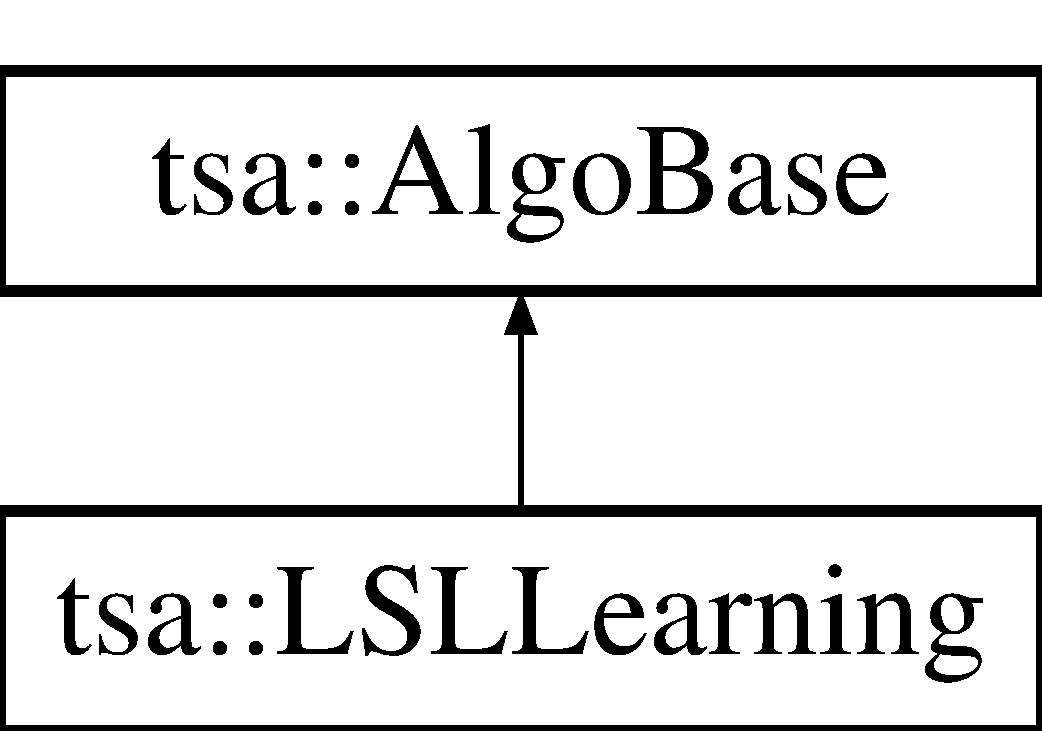
\includegraphics[height=2.000000cm]{classtsa_1_1_l_s_l_learning}
\end{center}
\end{figure}
\subsection*{Public Member Functions}
\begin{DoxyCompactItemize}
\item 
\hyperlink{classtsa_1_1_l_s_l_learning_ab1065fd9f61b44f25c4a9ee67e95dc1e}{L\+S\+L\+Learning} (unsigned int Order, double sigma, double lambda=1.\+0)
\item 
\hyperlink{classtsa_1_1_l_s_l_learning_ae1d9f9ea754c88bf19365c680ea2415a}{L\+S\+L\+Learning} (const \hyperlink{classtsa_1_1_l_s_l_learning}{L\+S\+L\+Learning} \&from)
\item 
\hyperlink{classtsa_1_1_l_s_l_learning_aab97f819bb4e1537621d9e84ee0bf140}{$\sim$\+L\+S\+L\+Learning} ()
\item 
\hyperlink{classtsa_1_1_l_s_l_learning}{L\+S\+L\+Learning} \& \hyperlink{classtsa_1_1_l_s_l_learning_a8b2b47d740bd2207f612e9c4aadaf220}{operator=} (const \hyperlink{classtsa_1_1_l_s_l_learning}{L\+S\+L\+Learning} \&from)
\item 
void \hyperlink{classtsa_1_1_l_s_l_learning_a0faa13eb2f31988b73c4740c3e1c4085}{Load} (const char $\ast$filename, const char $\ast$fmt=\char`\"{}txt\char`\"{})
\item 
void \hyperlink{classtsa_1_1_l_s_l_learning_aa3397a1d3944fb4ce19c612d74e7018a}{Save} (const char $\ast$filename, const char $\ast$fmt=\char`\"{}txt\char`\"{})
\item 
void \hyperlink{classtsa_1_1_l_s_l_learning_a54c30966b4ddf0327ef5f4b9a8b774f1}{xml\+\_\+serialize} (\hyperlink{classeternity_1_1xml__archive}{eternity\+::xml\+\_\+archive} \&xml, const char $\ast$p)
\end{DoxyCompactItemize}
\begin{Indent}\textbf{ Operations}\par
\begin{DoxyCompactItemize}
\item 
void \hyperlink{classtsa_1_1_l_s_l_learning_ac703af8aec35bece47d8b5dd5da96125}{operator()} (\hyperlink{namespacetsa_ac599574bcc094eda25613724b8f3ca9e}{Seq\+View\+Double} \&Input\+Data, \hyperlink{namespacetsa_ac599574bcc094eda25613724b8f3ca9e}{Seq\+View\+Double} \&Whitened\+Data)
\item 
void \hyperlink{classtsa_1_1_l_s_l_learning_a8a3c4b73d36808f940cd37fe8520d76f}{operator()} (\hyperlink{namespacetsa_ac599574bcc094eda25613724b8f3ca9e}{Seq\+View\+Double} \&Input\+Data, \hyperlink{classtsa_1_1_lattice_view}{Lattice\+View} \&Lat\+View)
\item 
void \hyperlink{classtsa_1_1_l_s_l_learning_adaf7049997744cc383427c0c673549f7}{operator()} (\hyperlink{namespacetsa_ac599574bcc094eda25613724b8f3ca9e}{Seq\+View\+Double} \&Input\+Data, \hyperlink{namespacetsa_a8900fb03d849baf447a1a0efe2561fb2}{Dvector} \&Parcor)
\item 
void \hyperlink{classtsa_1_1_l_s_l_learning_a9ec866ab1a8d8173e77519ce9f9855d5}{execute} (matrix\+\_\+row$<$ \hyperlink{namespacetsa_ad260cd21c1891c4ed391fe788569aba4}{Dmatrix} $>$ Input\+Data, matrix\+\_\+row$<$ \hyperlink{namespacetsa_ad260cd21c1891c4ed391fe788569aba4}{Dmatrix} $>$ Output\+Data)
\end{DoxyCompactItemize}
\end{Indent}
\begin{Indent}\textbf{ Getters}\par
\begin{DoxyCompactItemize}
\item 
unsigned int \hyperlink{classtsa_1_1_l_s_l_learning_ae442a68a9f2f455d86ce56342288381c}{Get\+Order} ()
\item 
double \hyperlink{classtsa_1_1_l_s_l_learning_acc051c6ae5281e916083fb80a21779e8}{Get\+Parcor\+Forward} (unsigned int j)
\item 
double \hyperlink{classtsa_1_1_l_s_l_learning_a276e9d2206da6c6ac89cdca1cd6c4560}{Get\+Parcor\+Backward} (unsigned int j)
\item 
double \hyperlink{classtsa_1_1_l_s_l_learning_ae012adf2bd5b2540f1a757113968a0d4}{Get\+Error\+Forward} (unsigned int i, unsigned int j)
\item 
double \hyperlink{classtsa_1_1_l_s_l_learning_af7f7b4d2830f2bdd66ab8210ef104480}{Get\+Error\+Backward} (unsigned int i, unsigned int j)
\item 
double \hyperlink{classtsa_1_1_l_s_l_learning_adaca2870907d65690fcaec01f4d96c95}{Get\+Epf} (unsigned int i, unsigned int j)
\item 
double \hyperlink{classtsa_1_1_l_s_l_learning_ad05ee328f1a40de4fc73bd9770ae08c2}{Get\+Epb} (unsigned int i, unsigned int j)
\item 
double \hyperlink{classtsa_1_1_l_s_l_learning_a41c8d09f732ae6fed7edaed61cd73ca2}{Get\+Gamma} (unsigned int j)
\item 
unsigned int \hyperlink{classtsa_1_1_l_s_l_learning_a03684c0760835f7cc8460561ea183f7e}{Get\+Status} ()
\item 
double \hyperlink{classtsa_1_1_l_s_l_learning_ac6f60dc86d296c35cba1582472d11d27}{Get\+Sigma} ()
\end{DoxyCompactItemize}
\end{Indent}
\subsection*{Private Attributes}
\begin{DoxyCompactItemize}
\item 
unsigned int \hyperlink{classtsa_1_1_l_s_l_learning_ae1e400504ab5fc285b4b2d740e4bde72}{m\+Order}
\item 
double \hyperlink{classtsa_1_1_l_s_l_learning_a6ba93296df7efc898844ff3ef645b287}{m\+Sigma}
\item 
\hyperlink{namespacetsa_ad260cd21c1891c4ed391fe788569aba4}{Dmatrix} \hyperlink{classtsa_1_1_l_s_l_learning_abc6dbb01c7f1a1b4c1d6ee5cb6ba14e8}{m\+EF}
\item 
\hyperlink{namespacetsa_ad260cd21c1891c4ed391fe788569aba4}{Dmatrix} \hyperlink{classtsa_1_1_l_s_l_learning_aee8f5369206276f3a7faaaaa048485fb}{m\+EB}
\item 
\hyperlink{namespacetsa_ad260cd21c1891c4ed391fe788569aba4}{Dmatrix} \hyperlink{classtsa_1_1_l_s_l_learning_a5cd2595571d70a64dfefbdd48dd96eb5}{m\+Epf}
\item 
\hyperlink{namespacetsa_ad260cd21c1891c4ed391fe788569aba4}{Dmatrix} \hyperlink{classtsa_1_1_l_s_l_learning_a4ccb655fdbbebb1a9875c6bc8238b373}{m\+Epb}
\item 
\hyperlink{namespacetsa_a8900fb03d849baf447a1a0efe2561fb2}{Dvector} \hyperlink{classtsa_1_1_l_s_l_learning_ad651adf83f8b9e770446ccf7f41fe61d}{m\+Kf}
\item 
\hyperlink{namespacetsa_a8900fb03d849baf447a1a0efe2561fb2}{Dvector} \hyperlink{classtsa_1_1_l_s_l_learning_ac895dcbb7407c99df7c8703e27b53ca4}{m\+Kb}
\item 
\hyperlink{namespacetsa_a8900fb03d849baf447a1a0efe2561fb2}{Dvector} \hyperlink{classtsa_1_1_l_s_l_learning_a4dc069522ea6f00876e144b7c26a8056}{mG}
\item 
double \hyperlink{classtsa_1_1_l_s_l_learning_a15b3df249118e9c6699a39a4b4add1db}{m\+Lambda}
\item 
unsigned int \hyperlink{classtsa_1_1_l_s_l_learning_ab1e86d5df54de8730402c123caccfd30}{m\+F0}
\end{DoxyCompactItemize}


\subsection{Detailed Description}
rithm for the learning phase of the Adaptive Least Squares Lattice 

Definition at line 74 of file L\+S\+L\+Learning.\+hpp.



\subsection{Constructor \& Destructor Documentation}
\mbox{\Hypertarget{classtsa_1_1_l_s_l_learning_ab1065fd9f61b44f25c4a9ee67e95dc1e}\label{classtsa_1_1_l_s_l_learning_ab1065fd9f61b44f25c4a9ee67e95dc1e}} 
\index{tsa\+::\+L\+S\+L\+Learning@{tsa\+::\+L\+S\+L\+Learning}!L\+S\+L\+Learning@{L\+S\+L\+Learning}}
\index{L\+S\+L\+Learning@{L\+S\+L\+Learning}!tsa\+::\+L\+S\+L\+Learning@{tsa\+::\+L\+S\+L\+Learning}}
\subsubsection{\texorpdfstring{L\+S\+L\+Learning()}{LSLLearning()}\hspace{0.1cm}{\footnotesize\ttfamily [1/2]}}
{\footnotesize\ttfamily tsa\+::\+L\+S\+L\+Learning\+::\+L\+S\+L\+Learning (\begin{DoxyParamCaption}\item[{unsigned int}]{Order,  }\item[{double}]{sigma,  }\item[{double}]{lambda = {\ttfamily 1.0} }\end{DoxyParamCaption})}

Constructor


\begin{DoxyParams}{Parameters}
{\em Order} & Order of the filter \\
\hline
{\em sigma} & guessed value for the initial sigma \\
\hline
{\em Lwsp} & Lenght of workspace \\
\hline
{\em lambda} & forgetting factor \\
\hline
\end{DoxyParams}


Definition at line 19 of file L\+S\+L\+Learning.\+cpp.

\mbox{\Hypertarget{classtsa_1_1_l_s_l_learning_ae1d9f9ea754c88bf19365c680ea2415a}\label{classtsa_1_1_l_s_l_learning_ae1d9f9ea754c88bf19365c680ea2415a}} 
\index{tsa\+::\+L\+S\+L\+Learning@{tsa\+::\+L\+S\+L\+Learning}!L\+S\+L\+Learning@{L\+S\+L\+Learning}}
\index{L\+S\+L\+Learning@{L\+S\+L\+Learning}!tsa\+::\+L\+S\+L\+Learning@{tsa\+::\+L\+S\+L\+Learning}}
\subsubsection{\texorpdfstring{L\+S\+L\+Learning()}{LSLLearning()}\hspace{0.1cm}{\footnotesize\ttfamily [2/2]}}
{\footnotesize\ttfamily tsa\+::\+L\+S\+L\+Learning\+::\+L\+S\+L\+Learning (\begin{DoxyParamCaption}\item[{const \hyperlink{classtsa_1_1_l_s_l_learning}{L\+S\+L\+Learning} \&}]{from }\end{DoxyParamCaption})}

Copy constructor


\begin{DoxyParams}{Parameters}
{\em from} & The instance that must be copied \\
\hline
\end{DoxyParams}


Definition at line 141 of file L\+S\+L\+Learning.\+cpp.

\mbox{\Hypertarget{classtsa_1_1_l_s_l_learning_aab97f819bb4e1537621d9e84ee0bf140}\label{classtsa_1_1_l_s_l_learning_aab97f819bb4e1537621d9e84ee0bf140}} 
\index{tsa\+::\+L\+S\+L\+Learning@{tsa\+::\+L\+S\+L\+Learning}!````~L\+S\+L\+Learning@{$\sim$\+L\+S\+L\+Learning}}
\index{````~L\+S\+L\+Learning@{$\sim$\+L\+S\+L\+Learning}!tsa\+::\+L\+S\+L\+Learning@{tsa\+::\+L\+S\+L\+Learning}}
\subsubsection{\texorpdfstring{$\sim$\+L\+S\+L\+Learning()}{~LSLLearning()}}
{\footnotesize\ttfamily tsa\+::\+L\+S\+L\+Learning\+::$\sim$\+L\+S\+L\+Learning (\begin{DoxyParamCaption}{ }\end{DoxyParamCaption})}

Destructor 

Definition at line 44 of file L\+S\+L\+Learning.\+cpp.



\subsection{Member Function Documentation}
\mbox{\Hypertarget{classtsa_1_1_l_s_l_learning_a9ec866ab1a8d8173e77519ce9f9855d5}\label{classtsa_1_1_l_s_l_learning_a9ec866ab1a8d8173e77519ce9f9855d5}} 
\index{tsa\+::\+L\+S\+L\+Learning@{tsa\+::\+L\+S\+L\+Learning}!execute@{execute}}
\index{execute@{execute}!tsa\+::\+L\+S\+L\+Learning@{tsa\+::\+L\+S\+L\+Learning}}
\subsubsection{\texorpdfstring{execute()}{execute()}}
{\footnotesize\ttfamily void tsa\+::\+L\+S\+L\+Learning\+::execute (\begin{DoxyParamCaption}\item[{matrix\+\_\+row$<$ \hyperlink{namespacetsa_ad260cd21c1891c4ed391fe788569aba4}{Dmatrix} $>$}]{Input\+Data,  }\item[{matrix\+\_\+row$<$ \hyperlink{namespacetsa_ad260cd21c1891c4ed391fe788569aba4}{Dmatrix} $>$}]{Output\+Data }\end{DoxyParamCaption})}


\begin{DoxyParams}{Parameters}
{\em Input\+Data} & Input data \\
\hline
{\em Output\+Data} & Output data \\
\hline
\end{DoxyParams}


Definition at line 101 of file L\+S\+L\+Learning.\+cpp.

\mbox{\Hypertarget{classtsa_1_1_l_s_l_learning_ad05ee328f1a40de4fc73bd9770ae08c2}\label{classtsa_1_1_l_s_l_learning_ad05ee328f1a40de4fc73bd9770ae08c2}} 
\index{tsa\+::\+L\+S\+L\+Learning@{tsa\+::\+L\+S\+L\+Learning}!Get\+Epb@{Get\+Epb}}
\index{Get\+Epb@{Get\+Epb}!tsa\+::\+L\+S\+L\+Learning@{tsa\+::\+L\+S\+L\+Learning}}
\subsubsection{\texorpdfstring{Get\+Epb()}{GetEpb()}}
{\footnotesize\ttfamily double tsa\+::\+L\+S\+L\+Learning\+::\+Get\+Epb (\begin{DoxyParamCaption}\item[{unsigned int}]{i,  }\item[{unsigned int}]{j }\end{DoxyParamCaption})\hspace{0.3cm}{\ttfamily [inline]}}



Definition at line 181 of file L\+S\+L\+Learning.\+hpp.

\mbox{\Hypertarget{classtsa_1_1_l_s_l_learning_adaca2870907d65690fcaec01f4d96c95}\label{classtsa_1_1_l_s_l_learning_adaca2870907d65690fcaec01f4d96c95}} 
\index{tsa\+::\+L\+S\+L\+Learning@{tsa\+::\+L\+S\+L\+Learning}!Get\+Epf@{Get\+Epf}}
\index{Get\+Epf@{Get\+Epf}!tsa\+::\+L\+S\+L\+Learning@{tsa\+::\+L\+S\+L\+Learning}}
\subsubsection{\texorpdfstring{Get\+Epf()}{GetEpf()}}
{\footnotesize\ttfamily double tsa\+::\+L\+S\+L\+Learning\+::\+Get\+Epf (\begin{DoxyParamCaption}\item[{unsigned int}]{i,  }\item[{unsigned int}]{j }\end{DoxyParamCaption})\hspace{0.3cm}{\ttfamily [inline]}}



Definition at line 175 of file L\+S\+L\+Learning.\+hpp.

\mbox{\Hypertarget{classtsa_1_1_l_s_l_learning_af7f7b4d2830f2bdd66ab8210ef104480}\label{classtsa_1_1_l_s_l_learning_af7f7b4d2830f2bdd66ab8210ef104480}} 
\index{tsa\+::\+L\+S\+L\+Learning@{tsa\+::\+L\+S\+L\+Learning}!Get\+Error\+Backward@{Get\+Error\+Backward}}
\index{Get\+Error\+Backward@{Get\+Error\+Backward}!tsa\+::\+L\+S\+L\+Learning@{tsa\+::\+L\+S\+L\+Learning}}
\subsubsection{\texorpdfstring{Get\+Error\+Backward()}{GetErrorBackward()}}
{\footnotesize\ttfamily double tsa\+::\+L\+S\+L\+Learning\+::\+Get\+Error\+Backward (\begin{DoxyParamCaption}\item[{unsigned int}]{i,  }\item[{unsigned int}]{j }\end{DoxyParamCaption})\hspace{0.3cm}{\ttfamily [inline]}}



Definition at line 171 of file L\+S\+L\+Learning.\+hpp.

\mbox{\Hypertarget{classtsa_1_1_l_s_l_learning_ae012adf2bd5b2540f1a757113968a0d4}\label{classtsa_1_1_l_s_l_learning_ae012adf2bd5b2540f1a757113968a0d4}} 
\index{tsa\+::\+L\+S\+L\+Learning@{tsa\+::\+L\+S\+L\+Learning}!Get\+Error\+Forward@{Get\+Error\+Forward}}
\index{Get\+Error\+Forward@{Get\+Error\+Forward}!tsa\+::\+L\+S\+L\+Learning@{tsa\+::\+L\+S\+L\+Learning}}
\subsubsection{\texorpdfstring{Get\+Error\+Forward()}{GetErrorForward()}}
{\footnotesize\ttfamily double tsa\+::\+L\+S\+L\+Learning\+::\+Get\+Error\+Forward (\begin{DoxyParamCaption}\item[{unsigned int}]{i,  }\item[{unsigned int}]{j }\end{DoxyParamCaption})\hspace{0.3cm}{\ttfamily [inline]}}



Definition at line 165 of file L\+S\+L\+Learning.\+hpp.

\mbox{\Hypertarget{classtsa_1_1_l_s_l_learning_a41c8d09f732ae6fed7edaed61cd73ca2}\label{classtsa_1_1_l_s_l_learning_a41c8d09f732ae6fed7edaed61cd73ca2}} 
\index{tsa\+::\+L\+S\+L\+Learning@{tsa\+::\+L\+S\+L\+Learning}!Get\+Gamma@{Get\+Gamma}}
\index{Get\+Gamma@{Get\+Gamma}!tsa\+::\+L\+S\+L\+Learning@{tsa\+::\+L\+S\+L\+Learning}}
\subsubsection{\texorpdfstring{Get\+Gamma()}{GetGamma()}}
{\footnotesize\ttfamily double tsa\+::\+L\+S\+L\+Learning\+::\+Get\+Gamma (\begin{DoxyParamCaption}\item[{unsigned int}]{j }\end{DoxyParamCaption})\hspace{0.3cm}{\ttfamily [inline]}}



Definition at line 185 of file L\+S\+L\+Learning.\+hpp.

\mbox{\Hypertarget{classtsa_1_1_l_s_l_learning_ae442a68a9f2f455d86ce56342288381c}\label{classtsa_1_1_l_s_l_learning_ae442a68a9f2f455d86ce56342288381c}} 
\index{tsa\+::\+L\+S\+L\+Learning@{tsa\+::\+L\+S\+L\+Learning}!Get\+Order@{Get\+Order}}
\index{Get\+Order@{Get\+Order}!tsa\+::\+L\+S\+L\+Learning@{tsa\+::\+L\+S\+L\+Learning}}
\subsubsection{\texorpdfstring{Get\+Order()}{GetOrder()}}
{\footnotesize\ttfamily unsigned int tsa\+::\+L\+S\+L\+Learning\+::\+Get\+Order (\begin{DoxyParamCaption}{ }\end{DoxyParamCaption})\hspace{0.3cm}{\ttfamily [inline]}}



Definition at line 150 of file L\+S\+L\+Learning.\+hpp.

\mbox{\Hypertarget{classtsa_1_1_l_s_l_learning_a276e9d2206da6c6ac89cdca1cd6c4560}\label{classtsa_1_1_l_s_l_learning_a276e9d2206da6c6ac89cdca1cd6c4560}} 
\index{tsa\+::\+L\+S\+L\+Learning@{tsa\+::\+L\+S\+L\+Learning}!Get\+Parcor\+Backward@{Get\+Parcor\+Backward}}
\index{Get\+Parcor\+Backward@{Get\+Parcor\+Backward}!tsa\+::\+L\+S\+L\+Learning@{tsa\+::\+L\+S\+L\+Learning}}
\subsubsection{\texorpdfstring{Get\+Parcor\+Backward()}{GetParcorBackward()}}
{\footnotesize\ttfamily double tsa\+::\+L\+S\+L\+Learning\+::\+Get\+Parcor\+Backward (\begin{DoxyParamCaption}\item[{unsigned int}]{j }\end{DoxyParamCaption})\hspace{0.3cm}{\ttfamily [inline]}}



Definition at line 161 of file L\+S\+L\+Learning.\+hpp.

\mbox{\Hypertarget{classtsa_1_1_l_s_l_learning_acc051c6ae5281e916083fb80a21779e8}\label{classtsa_1_1_l_s_l_learning_acc051c6ae5281e916083fb80a21779e8}} 
\index{tsa\+::\+L\+S\+L\+Learning@{tsa\+::\+L\+S\+L\+Learning}!Get\+Parcor\+Forward@{Get\+Parcor\+Forward}}
\index{Get\+Parcor\+Forward@{Get\+Parcor\+Forward}!tsa\+::\+L\+S\+L\+Learning@{tsa\+::\+L\+S\+L\+Learning}}
\subsubsection{\texorpdfstring{Get\+Parcor\+Forward()}{GetParcorForward()}}
{\footnotesize\ttfamily double tsa\+::\+L\+S\+L\+Learning\+::\+Get\+Parcor\+Forward (\begin{DoxyParamCaption}\item[{unsigned int}]{j }\end{DoxyParamCaption})\hspace{0.3cm}{\ttfamily [inline]}}



Definition at line 154 of file L\+S\+L\+Learning.\+hpp.

\mbox{\Hypertarget{classtsa_1_1_l_s_l_learning_ac6f60dc86d296c35cba1582472d11d27}\label{classtsa_1_1_l_s_l_learning_ac6f60dc86d296c35cba1582472d11d27}} 
\index{tsa\+::\+L\+S\+L\+Learning@{tsa\+::\+L\+S\+L\+Learning}!Get\+Sigma@{Get\+Sigma}}
\index{Get\+Sigma@{Get\+Sigma}!tsa\+::\+L\+S\+L\+Learning@{tsa\+::\+L\+S\+L\+Learning}}
\subsubsection{\texorpdfstring{Get\+Sigma()}{GetSigma()}}
{\footnotesize\ttfamily double tsa\+::\+L\+S\+L\+Learning\+::\+Get\+Sigma (\begin{DoxyParamCaption}{ }\end{DoxyParamCaption})\hspace{0.3cm}{\ttfamily [inline]}}



Definition at line 195 of file L\+S\+L\+Learning.\+hpp.

\mbox{\Hypertarget{classtsa_1_1_l_s_l_learning_a03684c0760835f7cc8460561ea183f7e}\label{classtsa_1_1_l_s_l_learning_a03684c0760835f7cc8460561ea183f7e}} 
\index{tsa\+::\+L\+S\+L\+Learning@{tsa\+::\+L\+S\+L\+Learning}!Get\+Status@{Get\+Status}}
\index{Get\+Status@{Get\+Status}!tsa\+::\+L\+S\+L\+Learning@{tsa\+::\+L\+S\+L\+Learning}}
\subsubsection{\texorpdfstring{Get\+Status()}{GetStatus()}}
{\footnotesize\ttfamily unsigned int tsa\+::\+L\+S\+L\+Learning\+::\+Get\+Status (\begin{DoxyParamCaption}{ }\end{DoxyParamCaption})\hspace{0.3cm}{\ttfamily [inline]}}



Definition at line 189 of file L\+S\+L\+Learning.\+hpp.

\mbox{\Hypertarget{classtsa_1_1_l_s_l_learning_a0faa13eb2f31988b73c4740c3e1c4085}\label{classtsa_1_1_l_s_l_learning_a0faa13eb2f31988b73c4740c3e1c4085}} 
\index{tsa\+::\+L\+S\+L\+Learning@{tsa\+::\+L\+S\+L\+Learning}!Load@{Load}}
\index{Load@{Load}!tsa\+::\+L\+S\+L\+Learning@{tsa\+::\+L\+S\+L\+Learning}}
\subsubsection{\texorpdfstring{Load()}{Load()}}
{\footnotesize\ttfamily void tsa\+::\+L\+S\+L\+Learning\+::\+Load (\begin{DoxyParamCaption}\item[{const char $\ast$}]{filename,  }\item[{const char $\ast$}]{fmt = {\ttfamily \char`\"{}txt\char`\"{}} }\end{DoxyParamCaption})\hspace{0.3cm}{\ttfamily [inline]}}



Definition at line 208 of file L\+S\+L\+Learning.\+hpp.

\mbox{\Hypertarget{classtsa_1_1_l_s_l_learning_ac703af8aec35bece47d8b5dd5da96125}\label{classtsa_1_1_l_s_l_learning_ac703af8aec35bece47d8b5dd5da96125}} 
\index{tsa\+::\+L\+S\+L\+Learning@{tsa\+::\+L\+S\+L\+Learning}!operator()@{operator()}}
\index{operator()@{operator()}!tsa\+::\+L\+S\+L\+Learning@{tsa\+::\+L\+S\+L\+Learning}}
\subsubsection{\texorpdfstring{operator()()}{operator()()}\hspace{0.1cm}{\footnotesize\ttfamily [1/3]}}
{\footnotesize\ttfamily void tsa\+::\+L\+S\+L\+Learning\+::operator() (\begin{DoxyParamCaption}\item[{\hyperlink{namespacetsa_ac599574bcc094eda25613724b8f3ca9e}{Seq\+View\+Double} \&}]{Input\+Data,  }\item[{\hyperlink{namespacetsa_ac599574bcc094eda25613724b8f3ca9e}{Seq\+View\+Double} \&}]{Whitened\+Data }\end{DoxyParamCaption})}


\begin{DoxyParams}{Parameters}
{\em Input\+Data} & Time series \\
\hline
{\em Whitened\+Data} & Whitened Time series \\
\hline
\end{DoxyParams}


Definition at line 47 of file L\+S\+L\+Learning.\+cpp.

\mbox{\Hypertarget{classtsa_1_1_l_s_l_learning_a8a3c4b73d36808f940cd37fe8520d76f}\label{classtsa_1_1_l_s_l_learning_a8a3c4b73d36808f940cd37fe8520d76f}} 
\index{tsa\+::\+L\+S\+L\+Learning@{tsa\+::\+L\+S\+L\+Learning}!operator()@{operator()}}
\index{operator()@{operator()}!tsa\+::\+L\+S\+L\+Learning@{tsa\+::\+L\+S\+L\+Learning}}
\subsubsection{\texorpdfstring{operator()()}{operator()()}\hspace{0.1cm}{\footnotesize\ttfamily [2/3]}}
{\footnotesize\ttfamily void tsa\+::\+L\+S\+L\+Learning\+::operator() (\begin{DoxyParamCaption}\item[{\hyperlink{namespacetsa_ac599574bcc094eda25613724b8f3ca9e}{Seq\+View\+Double} \&}]{Input\+Data,  }\item[{\hyperlink{classtsa_1_1_lattice_view}{Lattice\+View} \&}]{Lat\+View }\end{DoxyParamCaption})}


\begin{DoxyParams}{Parameters}
{\em Input\+Data} & \\
\hline
{\em Lat\+View} & \\
\hline
\end{DoxyParams}


Definition at line 63 of file L\+S\+L\+Learning.\+cpp.

\mbox{\Hypertarget{classtsa_1_1_l_s_l_learning_adaf7049997744cc383427c0c673549f7}\label{classtsa_1_1_l_s_l_learning_adaf7049997744cc383427c0c673549f7}} 
\index{tsa\+::\+L\+S\+L\+Learning@{tsa\+::\+L\+S\+L\+Learning}!operator()@{operator()}}
\index{operator()@{operator()}!tsa\+::\+L\+S\+L\+Learning@{tsa\+::\+L\+S\+L\+Learning}}
\subsubsection{\texorpdfstring{operator()()}{operator()()}\hspace{0.1cm}{\footnotesize\ttfamily [3/3]}}
{\footnotesize\ttfamily void tsa\+::\+L\+S\+L\+Learning\+::operator() (\begin{DoxyParamCaption}\item[{\hyperlink{namespacetsa_ac599574bcc094eda25613724b8f3ca9e}{Seq\+View\+Double} \&}]{Input\+Data,  }\item[{\hyperlink{namespacetsa_a8900fb03d849baf447a1a0efe2561fb2}{Dvector} \&}]{Parcor }\end{DoxyParamCaption})}


\begin{DoxyParams}{Parameters}
{\em Input\+Data} & \\
\hline
{\em Parcor} & \\
\hline
\end{DoxyParams}


Definition at line 84 of file L\+S\+L\+Learning.\+cpp.

\mbox{\Hypertarget{classtsa_1_1_l_s_l_learning_a8b2b47d740bd2207f612e9c4aadaf220}\label{classtsa_1_1_l_s_l_learning_a8b2b47d740bd2207f612e9c4aadaf220}} 
\index{tsa\+::\+L\+S\+L\+Learning@{tsa\+::\+L\+S\+L\+Learning}!operator=@{operator=}}
\index{operator=@{operator=}!tsa\+::\+L\+S\+L\+Learning@{tsa\+::\+L\+S\+L\+Learning}}
\subsubsection{\texorpdfstring{operator=()}{operator=()}}
{\footnotesize\ttfamily \hyperlink{classtsa_1_1_l_s_l_learning}{L\+S\+L\+Learning} \& tsa\+::\+L\+S\+L\+Learning\+::operator= (\begin{DoxyParamCaption}\item[{const \hyperlink{classtsa_1_1_l_s_l_learning}{L\+S\+L\+Learning} \&}]{from }\end{DoxyParamCaption})}

Assignement operator


\begin{DoxyParams}{Parameters}
{\em from} & The instance to be assigned from\\
\hline
\end{DoxyParams}
\begin{DoxyReturn}{Returns}
a reference to a new object 
\end{DoxyReturn}


Definition at line 152 of file L\+S\+L\+Learning.\+cpp.

\mbox{\Hypertarget{classtsa_1_1_l_s_l_learning_aa3397a1d3944fb4ce19c612d74e7018a}\label{classtsa_1_1_l_s_l_learning_aa3397a1d3944fb4ce19c612d74e7018a}} 
\index{tsa\+::\+L\+S\+L\+Learning@{tsa\+::\+L\+S\+L\+Learning}!Save@{Save}}
\index{Save@{Save}!tsa\+::\+L\+S\+L\+Learning@{tsa\+::\+L\+S\+L\+Learning}}
\subsubsection{\texorpdfstring{Save()}{Save()}}
{\footnotesize\ttfamily void tsa\+::\+L\+S\+L\+Learning\+::\+Save (\begin{DoxyParamCaption}\item[{const char $\ast$}]{filename,  }\item[{const char $\ast$}]{fmt = {\ttfamily \char`\"{}txt\char`\"{}} }\end{DoxyParamCaption})\hspace{0.3cm}{\ttfamily [inline]}}



Definition at line 215 of file L\+S\+L\+Learning.\+hpp.

\mbox{\Hypertarget{classtsa_1_1_l_s_l_learning_a54c30966b4ddf0327ef5f4b9a8b774f1}\label{classtsa_1_1_l_s_l_learning_a54c30966b4ddf0327ef5f4b9a8b774f1}} 
\index{tsa\+::\+L\+S\+L\+Learning@{tsa\+::\+L\+S\+L\+Learning}!xml\+\_\+serialize@{xml\+\_\+serialize}}
\index{xml\+\_\+serialize@{xml\+\_\+serialize}!tsa\+::\+L\+S\+L\+Learning@{tsa\+::\+L\+S\+L\+Learning}}
\subsubsection{\texorpdfstring{xml\+\_\+serialize()}{xml\_serialize()}}
{\footnotesize\ttfamily void tsa\+::\+L\+S\+L\+Learning\+::xml\+\_\+serialize (\begin{DoxyParamCaption}\item[{\hyperlink{classeternity_1_1xml__archive}{eternity\+::xml\+\_\+archive} \&}]{xml,  }\item[{const char $\ast$}]{p }\end{DoxyParamCaption})\hspace{0.3cm}{\ttfamily [inline]}}



Definition at line 222 of file L\+S\+L\+Learning.\+hpp.



\subsection{Member Data Documentation}
\mbox{\Hypertarget{classtsa_1_1_l_s_l_learning_aee8f5369206276f3a7faaaaa048485fb}\label{classtsa_1_1_l_s_l_learning_aee8f5369206276f3a7faaaaa048485fb}} 
\index{tsa\+::\+L\+S\+L\+Learning@{tsa\+::\+L\+S\+L\+Learning}!m\+EB@{m\+EB}}
\index{m\+EB@{m\+EB}!tsa\+::\+L\+S\+L\+Learning@{tsa\+::\+L\+S\+L\+Learning}}
\subsubsection{\texorpdfstring{m\+EB}{mEB}}
{\footnotesize\ttfamily \hyperlink{namespacetsa_ad260cd21c1891c4ed391fe788569aba4}{Dmatrix} tsa\+::\+L\+S\+L\+Learning\+::m\+EB\hspace{0.3cm}{\ttfamily [private]}}

Error\+Backward 

Definition at line 267 of file L\+S\+L\+Learning.\+hpp.

\mbox{\Hypertarget{classtsa_1_1_l_s_l_learning_abc6dbb01c7f1a1b4c1d6ee5cb6ba14e8}\label{classtsa_1_1_l_s_l_learning_abc6dbb01c7f1a1b4c1d6ee5cb6ba14e8}} 
\index{tsa\+::\+L\+S\+L\+Learning@{tsa\+::\+L\+S\+L\+Learning}!m\+EF@{m\+EF}}
\index{m\+EF@{m\+EF}!tsa\+::\+L\+S\+L\+Learning@{tsa\+::\+L\+S\+L\+Learning}}
\subsubsection{\texorpdfstring{m\+EF}{mEF}}
{\footnotesize\ttfamily \hyperlink{namespacetsa_ad260cd21c1891c4ed391fe788569aba4}{Dmatrix} tsa\+::\+L\+S\+L\+Learning\+::m\+EF\hspace{0.3cm}{\ttfamily [private]}}

Error\+Forward 

Definition at line 266 of file L\+S\+L\+Learning.\+hpp.

\mbox{\Hypertarget{classtsa_1_1_l_s_l_learning_a4ccb655fdbbebb1a9875c6bc8238b373}\label{classtsa_1_1_l_s_l_learning_a4ccb655fdbbebb1a9875c6bc8238b373}} 
\index{tsa\+::\+L\+S\+L\+Learning@{tsa\+::\+L\+S\+L\+Learning}!m\+Epb@{m\+Epb}}
\index{m\+Epb@{m\+Epb}!tsa\+::\+L\+S\+L\+Learning@{tsa\+::\+L\+S\+L\+Learning}}
\subsubsection{\texorpdfstring{m\+Epb}{mEpb}}
{\footnotesize\ttfamily \hyperlink{namespacetsa_ad260cd21c1891c4ed391fe788569aba4}{Dmatrix} tsa\+::\+L\+S\+L\+Learning\+::m\+Epb\hspace{0.3cm}{\ttfamily [private]}}

Mean \hyperlink{classtsa_1_1_square}{Square} Error Backward 

Definition at line 269 of file L\+S\+L\+Learning.\+hpp.

\mbox{\Hypertarget{classtsa_1_1_l_s_l_learning_a5cd2595571d70a64dfefbdd48dd96eb5}\label{classtsa_1_1_l_s_l_learning_a5cd2595571d70a64dfefbdd48dd96eb5}} 
\index{tsa\+::\+L\+S\+L\+Learning@{tsa\+::\+L\+S\+L\+Learning}!m\+Epf@{m\+Epf}}
\index{m\+Epf@{m\+Epf}!tsa\+::\+L\+S\+L\+Learning@{tsa\+::\+L\+S\+L\+Learning}}
\subsubsection{\texorpdfstring{m\+Epf}{mEpf}}
{\footnotesize\ttfamily \hyperlink{namespacetsa_ad260cd21c1891c4ed391fe788569aba4}{Dmatrix} tsa\+::\+L\+S\+L\+Learning\+::m\+Epf\hspace{0.3cm}{\ttfamily [private]}}

Mean \hyperlink{classtsa_1_1_square}{Square} Error Forward 

Definition at line 268 of file L\+S\+L\+Learning.\+hpp.

\mbox{\Hypertarget{classtsa_1_1_l_s_l_learning_ab1e86d5df54de8730402c123caccfd30}\label{classtsa_1_1_l_s_l_learning_ab1e86d5df54de8730402c123caccfd30}} 
\index{tsa\+::\+L\+S\+L\+Learning@{tsa\+::\+L\+S\+L\+Learning}!m\+F0@{m\+F0}}
\index{m\+F0@{m\+F0}!tsa\+::\+L\+S\+L\+Learning@{tsa\+::\+L\+S\+L\+Learning}}
\subsubsection{\texorpdfstring{m\+F0}{mF0}}
{\footnotesize\ttfamily unsigned int tsa\+::\+L\+S\+L\+Learning\+::m\+F0\hspace{0.3cm}{\ttfamily [private]}}

index for the status of the Lattice filter 

Definition at line 274 of file L\+S\+L\+Learning.\+hpp.

\mbox{\Hypertarget{classtsa_1_1_l_s_l_learning_a4dc069522ea6f00876e144b7c26a8056}\label{classtsa_1_1_l_s_l_learning_a4dc069522ea6f00876e144b7c26a8056}} 
\index{tsa\+::\+L\+S\+L\+Learning@{tsa\+::\+L\+S\+L\+Learning}!mG@{mG}}
\index{mG@{mG}!tsa\+::\+L\+S\+L\+Learning@{tsa\+::\+L\+S\+L\+Learning}}
\subsubsection{\texorpdfstring{mG}{mG}}
{\footnotesize\ttfamily \hyperlink{namespacetsa_a8900fb03d849baf447a1a0efe2561fb2}{Dvector} tsa\+::\+L\+S\+L\+Learning\+::mG\hspace{0.3cm}{\ttfamily [private]}}

Angle parameter 

Definition at line 272 of file L\+S\+L\+Learning.\+hpp.

\mbox{\Hypertarget{classtsa_1_1_l_s_l_learning_ac895dcbb7407c99df7c8703e27b53ca4}\label{classtsa_1_1_l_s_l_learning_ac895dcbb7407c99df7c8703e27b53ca4}} 
\index{tsa\+::\+L\+S\+L\+Learning@{tsa\+::\+L\+S\+L\+Learning}!m\+Kb@{m\+Kb}}
\index{m\+Kb@{m\+Kb}!tsa\+::\+L\+S\+L\+Learning@{tsa\+::\+L\+S\+L\+Learning}}
\subsubsection{\texorpdfstring{m\+Kb}{mKb}}
{\footnotesize\ttfamily \hyperlink{namespacetsa_a8900fb03d849baf447a1a0efe2561fb2}{Dvector} tsa\+::\+L\+S\+L\+Learning\+::m\+Kb\hspace{0.3cm}{\ttfamily [private]}}

Backward Parcor 

Definition at line 271 of file L\+S\+L\+Learning.\+hpp.

\mbox{\Hypertarget{classtsa_1_1_l_s_l_learning_ad651adf83f8b9e770446ccf7f41fe61d}\label{classtsa_1_1_l_s_l_learning_ad651adf83f8b9e770446ccf7f41fe61d}} 
\index{tsa\+::\+L\+S\+L\+Learning@{tsa\+::\+L\+S\+L\+Learning}!m\+Kf@{m\+Kf}}
\index{m\+Kf@{m\+Kf}!tsa\+::\+L\+S\+L\+Learning@{tsa\+::\+L\+S\+L\+Learning}}
\subsubsection{\texorpdfstring{m\+Kf}{mKf}}
{\footnotesize\ttfamily \hyperlink{namespacetsa_a8900fb03d849baf447a1a0efe2561fb2}{Dvector} tsa\+::\+L\+S\+L\+Learning\+::m\+Kf\hspace{0.3cm}{\ttfamily [private]}}

Forward Parcor 

Definition at line 270 of file L\+S\+L\+Learning.\+hpp.

\mbox{\Hypertarget{classtsa_1_1_l_s_l_learning_a15b3df249118e9c6699a39a4b4add1db}\label{classtsa_1_1_l_s_l_learning_a15b3df249118e9c6699a39a4b4add1db}} 
\index{tsa\+::\+L\+S\+L\+Learning@{tsa\+::\+L\+S\+L\+Learning}!m\+Lambda@{m\+Lambda}}
\index{m\+Lambda@{m\+Lambda}!tsa\+::\+L\+S\+L\+Learning@{tsa\+::\+L\+S\+L\+Learning}}
\subsubsection{\texorpdfstring{m\+Lambda}{mLambda}}
{\footnotesize\ttfamily double tsa\+::\+L\+S\+L\+Learning\+::m\+Lambda\hspace{0.3cm}{\ttfamily [private]}}

Forgetting Factor 

Definition at line 273 of file L\+S\+L\+Learning.\+hpp.

\mbox{\Hypertarget{classtsa_1_1_l_s_l_learning_ae1e400504ab5fc285b4b2d740e4bde72}\label{classtsa_1_1_l_s_l_learning_ae1e400504ab5fc285b4b2d740e4bde72}} 
\index{tsa\+::\+L\+S\+L\+Learning@{tsa\+::\+L\+S\+L\+Learning}!m\+Order@{m\+Order}}
\index{m\+Order@{m\+Order}!tsa\+::\+L\+S\+L\+Learning@{tsa\+::\+L\+S\+L\+Learning}}
\subsubsection{\texorpdfstring{m\+Order}{mOrder}}
{\footnotesize\ttfamily unsigned int tsa\+::\+L\+S\+L\+Learning\+::m\+Order\hspace{0.3cm}{\ttfamily [private]}}

Order of the filter 

Definition at line 264 of file L\+S\+L\+Learning.\+hpp.

\mbox{\Hypertarget{classtsa_1_1_l_s_l_learning_a6ba93296df7efc898844ff3ef645b287}\label{classtsa_1_1_l_s_l_learning_a6ba93296df7efc898844ff3ef645b287}} 
\index{tsa\+::\+L\+S\+L\+Learning@{tsa\+::\+L\+S\+L\+Learning}!m\+Sigma@{m\+Sigma}}
\index{m\+Sigma@{m\+Sigma}!tsa\+::\+L\+S\+L\+Learning@{tsa\+::\+L\+S\+L\+Learning}}
\subsubsection{\texorpdfstring{m\+Sigma}{mSigma}}
{\footnotesize\ttfamily double tsa\+::\+L\+S\+L\+Learning\+::m\+Sigma\hspace{0.3cm}{\ttfamily [private]}}

The estimated rms 

Definition at line 265 of file L\+S\+L\+Learning.\+hpp.



The documentation for this class was generated from the following files\+:\begin{DoxyCompactItemize}
\item 
/home/filip/\+Ph\+D/\+W\+D\+F\+Pipe\+\_\+test/p4\+T\+S\+A/include/\hyperlink{_l_s_l_learning_8hpp}{L\+S\+L\+Learning.\+hpp}\item 
/home/filip/\+Ph\+D/\+W\+D\+F\+Pipe\+\_\+test/p4\+T\+S\+A/src/\hyperlink{_l_s_l_learning_8cpp}{L\+S\+L\+Learning.\+cpp}\end{DoxyCompactItemize}

\hypertarget{classtsa_1_1_math_utils}{}\section{tsa\+:\+:Math\+Utils Class Reference}
\label{classtsa_1_1_math_utils}\index{tsa\+::\+Math\+Utils@{tsa\+::\+Math\+Utils}}


{\ttfamily \#include $<$tsa\+Utility\+Functions.\+hpp$>$}

\subsection*{Static Public Member Functions}
\begin{DoxyCompactItemize}
\item 
static unsigned int \hyperlink{classtsa_1_1_math_utils_a4d4f3e95ae31cf490baec26aa6babba6}{isqrt} (unsigned long val)
\item 
static int \hyperlink{classtsa_1_1_math_utils_a4edc4a9fbd224706b312200fadfd6e6e}{gcd} (int u, int v)
\item 
static int \hyperlink{classtsa_1_1_math_utils_a52fe9c7e80f1facb7dd118491786ad27}{max} (int u, int v)
\item 
static int \hyperlink{classtsa_1_1_math_utils_a00386ddcb986eea58d68e5fb2e4bd9f1}{min} (int u, int v)
\end{DoxyCompactItemize}


\subsection{Detailed Description}


Definition at line 140 of file tsa\+Utility\+Functions.\+hpp.



\subsection{Member Function Documentation}
\mbox{\Hypertarget{classtsa_1_1_math_utils_a4edc4a9fbd224706b312200fadfd6e6e}\label{classtsa_1_1_math_utils_a4edc4a9fbd224706b312200fadfd6e6e}} 
\index{tsa\+::\+Math\+Utils@{tsa\+::\+Math\+Utils}!gcd@{gcd}}
\index{gcd@{gcd}!tsa\+::\+Math\+Utils@{tsa\+::\+Math\+Utils}}
\subsubsection{\texorpdfstring{gcd()}{gcd()}}
{\footnotesize\ttfamily static int tsa\+::\+Math\+Utils\+::gcd (\begin{DoxyParamCaption}\item[{int}]{u,  }\item[{int}]{v }\end{DoxyParamCaption})\hspace{0.3cm}{\ttfamily [inline]}, {\ttfamily [static]}}

Find the great common divisor between two numbers u and v


\begin{DoxyParams}{Parameters}
{\em u} & first number \\
\hline
{\em v} & second number\\
\hline
\end{DoxyParams}
\begin{DoxyReturn}{Returns}
the great common divisor between u and v 
\end{DoxyReturn}


Definition at line 169 of file tsa\+Utility\+Functions.\+hpp.

\mbox{\Hypertarget{classtsa_1_1_math_utils_a4d4f3e95ae31cf490baec26aa6babba6}\label{classtsa_1_1_math_utils_a4d4f3e95ae31cf490baec26aa6babba6}} 
\index{tsa\+::\+Math\+Utils@{tsa\+::\+Math\+Utils}!isqrt@{isqrt}}
\index{isqrt@{isqrt}!tsa\+::\+Math\+Utils@{tsa\+::\+Math\+Utils}}
\subsubsection{\texorpdfstring{isqrt()}{isqrt()}}
{\footnotesize\ttfamily static unsigned int tsa\+::\+Math\+Utils\+::isqrt (\begin{DoxyParamCaption}\item[{unsigned long}]{val }\end{DoxyParamCaption})\hspace{0.3cm}{\ttfamily [inline]}, {\ttfamily [static]}}

Evaluate the integer square root of a number.


\begin{DoxyParams}{Parameters}
{\em val} & input number\\
\hline
\end{DoxyParams}
\begin{DoxyReturn}{Returns}
integer square root of val 
\end{DoxyReturn}


Definition at line 150 of file tsa\+Utility\+Functions.\+hpp.

\mbox{\Hypertarget{classtsa_1_1_math_utils_a52fe9c7e80f1facb7dd118491786ad27}\label{classtsa_1_1_math_utils_a52fe9c7e80f1facb7dd118491786ad27}} 
\index{tsa\+::\+Math\+Utils@{tsa\+::\+Math\+Utils}!max@{max}}
\index{max@{max}!tsa\+::\+Math\+Utils@{tsa\+::\+Math\+Utils}}
\subsubsection{\texorpdfstring{max()}{max()}}
{\footnotesize\ttfamily static int tsa\+::\+Math\+Utils\+::max (\begin{DoxyParamCaption}\item[{int}]{u,  }\item[{int}]{v }\end{DoxyParamCaption})\hspace{0.3cm}{\ttfamily [inline]}, {\ttfamily [static]}}



Definition at line 182 of file tsa\+Utility\+Functions.\+hpp.

\mbox{\Hypertarget{classtsa_1_1_math_utils_a00386ddcb986eea58d68e5fb2e4bd9f1}\label{classtsa_1_1_math_utils_a00386ddcb986eea58d68e5fb2e4bd9f1}} 
\index{tsa\+::\+Math\+Utils@{tsa\+::\+Math\+Utils}!min@{min}}
\index{min@{min}!tsa\+::\+Math\+Utils@{tsa\+::\+Math\+Utils}}
\subsubsection{\texorpdfstring{min()}{min()}}
{\footnotesize\ttfamily static int tsa\+::\+Math\+Utils\+::min (\begin{DoxyParamCaption}\item[{int}]{u,  }\item[{int}]{v }\end{DoxyParamCaption})\hspace{0.3cm}{\ttfamily [inline]}, {\ttfamily [static]}}



Definition at line 186 of file tsa\+Utility\+Functions.\+hpp.



The documentation for this class was generated from the following file\+:\begin{DoxyCompactItemize}
\item 
/home/filip/\+Ph\+D/\+W\+D\+F\+Pipe\+\_\+test/p4\+T\+S\+A/include/\hyperlink{tsa_utility_functions_8hpp}{tsa\+Utility\+Functions.\+hpp}\end{DoxyCompactItemize}

\hypertarget{class_m_f_carchive}{}\section{M\+F\+Carchive Class Reference}
\label{class_m_f_carchive}\index{M\+F\+Carchive@{M\+F\+Carchive}}


{\ttfamily \#include $<$M\+F\+C\+Archive.\+h$>$}

Inheritance diagram for M\+F\+Carchive\+:\begin{figure}[H]
\begin{center}
\leavevmode
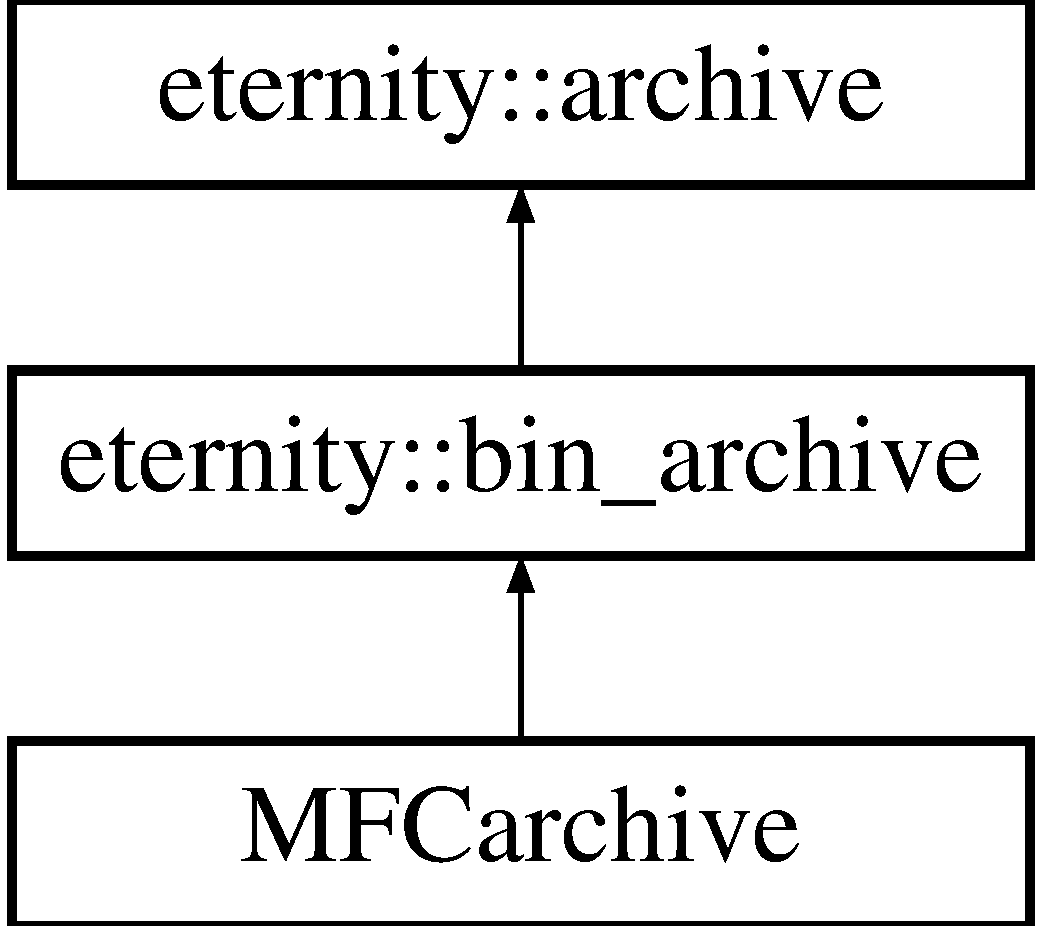
\includegraphics[height=3.000000cm]{class_m_f_carchive}
\end{center}
\end{figure}
\subsection*{Public Member Functions}
\begin{DoxyCompactItemize}
\item 
virtual size\+\_\+t \hyperlink{class_m_f_carchive_a8c5191701a84b9a4d2812887cfc28651}{write} (const void $\ast$buffer, size\+\_\+t size, size\+\_\+t count)
\begin{DoxyCompactList}\small\item\em write a buffer of a certain legnth n time in the archive \end{DoxyCompactList}\item 
virtual size\+\_\+t \hyperlink{class_m_f_carchive_a175a083e8f81fe490714be920539f7b9}{read} (void $\ast$buffer, size\+\_\+t size, size\+\_\+t count)
\begin{DoxyCompactList}\small\item\em read a buffer of a certain legnth n time in the archive \end{DoxyCompactList}\item 
\hyperlink{class_m_f_carchive_adf62fabd21e51cf0f9e1a50fc0367201}{M\+F\+Carchive} (Carchive \&ar)
\item 
virtual \hyperlink{class_m_f_carchive_aa328aff9303e279909cc3855019fdd73}{$\sim$\+M\+F\+Carchive} ()
\end{DoxyCompactItemize}
\subsection*{Protected Attributes}
\begin{DoxyCompactItemize}
\item 
Carchive \& \hyperlink{class_m_f_carchive_a57d8f21676284f6004ce3ca11b573c05}{m\+\_\+ar}
\end{DoxyCompactItemize}
\subsection*{Additional Inherited Members}


\subsection{Detailed Description}


Definition at line 36 of file M\+F\+C\+Archive.\+h.



\subsection{Constructor \& Destructor Documentation}
\mbox{\Hypertarget{class_m_f_carchive_adf62fabd21e51cf0f9e1a50fc0367201}\label{class_m_f_carchive_adf62fabd21e51cf0f9e1a50fc0367201}} 
\index{M\+F\+Carchive@{M\+F\+Carchive}!M\+F\+Carchive@{M\+F\+Carchive}}
\index{M\+F\+Carchive@{M\+F\+Carchive}!M\+F\+Carchive@{M\+F\+Carchive}}
\subsubsection{\texorpdfstring{M\+F\+Carchive()}{MFCarchive()}}
{\footnotesize\ttfamily M\+F\+Carchive\+::\+M\+F\+Carchive (\begin{DoxyParamCaption}\item[{Carchive \&}]{ar }\end{DoxyParamCaption})}



Definition at line 39 of file M\+F\+C\+Archive.\+cpp.

\mbox{\Hypertarget{class_m_f_carchive_aa328aff9303e279909cc3855019fdd73}\label{class_m_f_carchive_aa328aff9303e279909cc3855019fdd73}} 
\index{M\+F\+Carchive@{M\+F\+Carchive}!````~M\+F\+Carchive@{$\sim$\+M\+F\+Carchive}}
\index{````~M\+F\+Carchive@{$\sim$\+M\+F\+Carchive}!M\+F\+Carchive@{M\+F\+Carchive}}
\subsubsection{\texorpdfstring{$\sim$\+M\+F\+Carchive()}{~MFCarchive()}}
{\footnotesize\ttfamily virtual M\+F\+Carchive\+::$\sim$\+M\+F\+Carchive (\begin{DoxyParamCaption}{ }\end{DoxyParamCaption})\hspace{0.3cm}{\ttfamily [inline]}, {\ttfamily [virtual]}}



Definition at line 43 of file M\+F\+C\+Archive.\+h.



\subsection{Member Function Documentation}
\mbox{\Hypertarget{class_m_f_carchive_a175a083e8f81fe490714be920539f7b9}\label{class_m_f_carchive_a175a083e8f81fe490714be920539f7b9}} 
\index{M\+F\+Carchive@{M\+F\+Carchive}!read@{read}}
\index{read@{read}!M\+F\+Carchive@{M\+F\+Carchive}}
\subsubsection{\texorpdfstring{read()}{read()}}
{\footnotesize\ttfamily size\+\_\+t M\+F\+Carchive\+::read (\begin{DoxyParamCaption}\item[{void $\ast$}]{buffer,  }\item[{size\+\_\+t}]{size,  }\item[{size\+\_\+t}]{count }\end{DoxyParamCaption})\hspace{0.3cm}{\ttfamily [virtual]}}



read a buffer of a certain legnth n time in the archive 



Implements \hyperlink{classeternity_1_1bin__archive_a5d67b032541f5a1e104d2fcd0eaa7a55}{eternity\+::bin\+\_\+archive}.



Definition at line 49 of file M\+F\+C\+Archive.\+cpp.

\mbox{\Hypertarget{class_m_f_carchive_a8c5191701a84b9a4d2812887cfc28651}\label{class_m_f_carchive_a8c5191701a84b9a4d2812887cfc28651}} 
\index{M\+F\+Carchive@{M\+F\+Carchive}!write@{write}}
\index{write@{write}!M\+F\+Carchive@{M\+F\+Carchive}}
\subsubsection{\texorpdfstring{write()}{write()}}
{\footnotesize\ttfamily size\+\_\+t M\+F\+Carchive\+::write (\begin{DoxyParamCaption}\item[{const void $\ast$}]{buffer,  }\item[{size\+\_\+t}]{size,  }\item[{size\+\_\+t}]{count }\end{DoxyParamCaption})\hspace{0.3cm}{\ttfamily [virtual]}}



write a buffer of a certain legnth n time in the archive 



Implements \hyperlink{classeternity_1_1bin__archive_acbe041b0815f2721ee18ad042557b14e}{eternity\+::bin\+\_\+archive}.



Definition at line 44 of file M\+F\+C\+Archive.\+cpp.



\subsection{Member Data Documentation}
\mbox{\Hypertarget{class_m_f_carchive_a57d8f21676284f6004ce3ca11b573c05}\label{class_m_f_carchive_a57d8f21676284f6004ce3ca11b573c05}} 
\index{M\+F\+Carchive@{M\+F\+Carchive}!m\+\_\+ar@{m\+\_\+ar}}
\index{m\+\_\+ar@{m\+\_\+ar}!M\+F\+Carchive@{M\+F\+Carchive}}
\subsubsection{\texorpdfstring{m\+\_\+ar}{m\_ar}}
{\footnotesize\ttfamily Carchive\& M\+F\+Carchive\+::m\+\_\+ar\hspace{0.3cm}{\ttfamily [protected]}}



Definition at line 46 of file M\+F\+C\+Archive.\+h.



The documentation for this class was generated from the following files\+:\begin{DoxyCompactItemize}
\item 
/home/filip/\+Ph\+D/\+W\+D\+F\+Pipe\+\_\+test/p4\+T\+S\+A/include/eternity/\hyperlink{_m_f_c_archive_8h}{M\+F\+C\+Archive.\+h}\item 
/home/filip/\+Ph\+D/\+W\+D\+F\+Pipe\+\_\+test/p4\+T\+S\+A/include/eternity/mfc/\hyperlink{_m_f_c_archive_8cpp}{M\+F\+C\+Archive.\+cpp}\end{DoxyCompactItemize}

\hypertarget{classtsa_1_1missing__data}{}\section{tsa\+:\+:missing\+\_\+data Class Reference}
\label{classtsa_1_1missing__data}\index{tsa\+::missing\+\_\+data@{tsa\+::missing\+\_\+data}}


{\ttfamily \#include $<$Algo\+Exceptions.\+hpp$>$}

Inheritance diagram for tsa\+:\+:missing\+\_\+data\+:\begin{figure}[H]
\begin{center}
\leavevmode
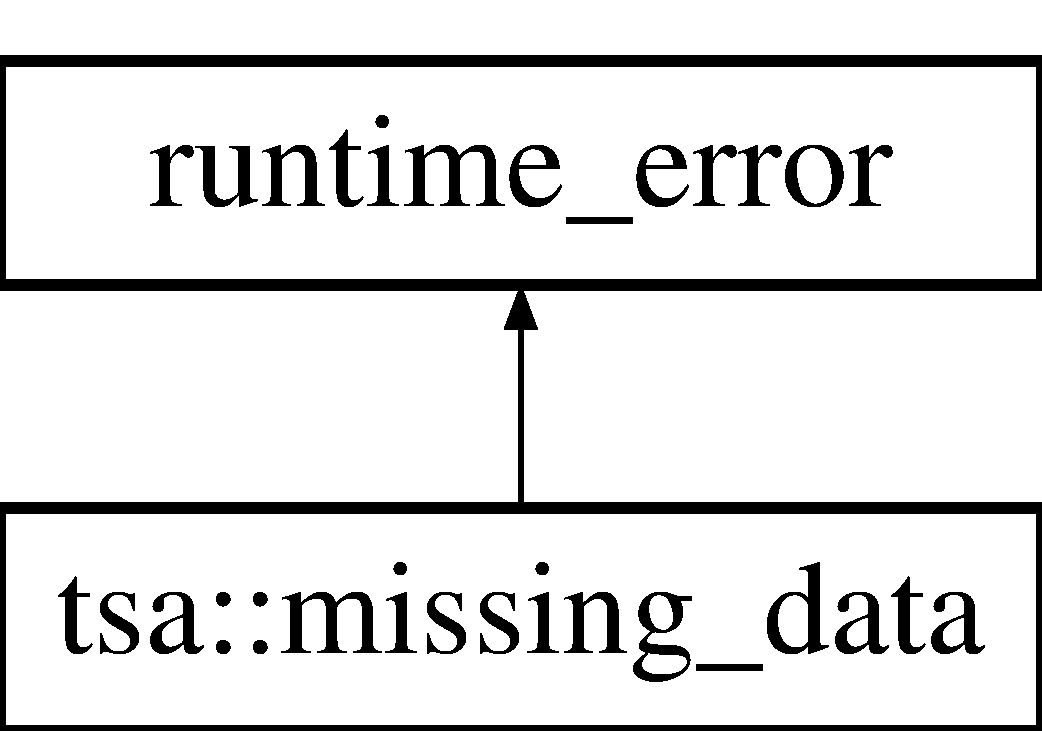
\includegraphics[height=2.000000cm]{classtsa_1_1missing__data}
\end{center}
\end{figure}
\subsection*{Public Member Functions}
\begin{DoxyCompactItemize}
\item 
\hyperlink{classtsa_1_1missing__data_a8d5ae46c22478ec86fae022f0044d2b7}{missing\+\_\+data} (const std\+::string \&msg, double miss\+\_\+start, double miss\+\_\+end, unsigned int channel)
\item 
double \hyperlink{classtsa_1_1missing__data_a14e20caa0f0f2baf341625d09e9da157}{Start} ()
\item 
double \hyperlink{classtsa_1_1missing__data_a10c01ad5fd1fd4bc26d69114cb90ee08}{End} ()
\item 
double \hyperlink{classtsa_1_1missing__data_a96f7fd1c113289c1cfd22117fda3ec83}{Channel} ()
\end{DoxyCompactItemize}
\subsection*{Private Attributes}
\begin{DoxyCompactItemize}
\item 
double \hyperlink{classtsa_1_1missing__data_a3bb2ac2dd0703730e7f0b29037bf65aa}{m\+Start\+Period}
\item 
double \hyperlink{classtsa_1_1missing__data_ae4ac26763b09836066dd3202f421a2cc}{m\+End\+Period}
\item 
unsigned int \hyperlink{classtsa_1_1missing__data_ac223001a840eeb59c73cb0cef2483ed2}{m\+Channel}
\end{DoxyCompactItemize}


\subsection{Detailed Description}
This exception should be used when some frames are missing 

Definition at line 168 of file Algo\+Exceptions.\+hpp.



\subsection{Constructor \& Destructor Documentation}
\mbox{\Hypertarget{classtsa_1_1missing__data_a8d5ae46c22478ec86fae022f0044d2b7}\label{classtsa_1_1missing__data_a8d5ae46c22478ec86fae022f0044d2b7}} 
\index{tsa\+::missing\+\_\+data@{tsa\+::missing\+\_\+data}!missing\+\_\+data@{missing\+\_\+data}}
\index{missing\+\_\+data@{missing\+\_\+data}!tsa\+::missing\+\_\+data@{tsa\+::missing\+\_\+data}}
\subsubsection{\texorpdfstring{missing\+\_\+data()}{missing\_data()}}
{\footnotesize\ttfamily tsa\+::missing\+\_\+data\+::missing\+\_\+data (\begin{DoxyParamCaption}\item[{const std\+::string \&}]{msg,  }\item[{double}]{miss\+\_\+start,  }\item[{double}]{miss\+\_\+end,  }\item[{unsigned int}]{channel }\end{DoxyParamCaption})\hspace{0.3cm}{\ttfamily [inline]}}

Constructor


\begin{DoxyParams}{Parameters}
{\em msg} & error message \\
\hline
\end{DoxyParams}


Definition at line 176 of file Algo\+Exceptions.\+hpp.



\subsection{Member Function Documentation}
\mbox{\Hypertarget{classtsa_1_1missing__data_a96f7fd1c113289c1cfd22117fda3ec83}\label{classtsa_1_1missing__data_a96f7fd1c113289c1cfd22117fda3ec83}} 
\index{tsa\+::missing\+\_\+data@{tsa\+::missing\+\_\+data}!Channel@{Channel}}
\index{Channel@{Channel}!tsa\+::missing\+\_\+data@{tsa\+::missing\+\_\+data}}
\subsubsection{\texorpdfstring{Channel()}{Channel()}}
{\footnotesize\ttfamily double tsa\+::missing\+\_\+data\+::\+Channel (\begin{DoxyParamCaption}{ }\end{DoxyParamCaption})\hspace{0.3cm}{\ttfamily [inline]}}



Definition at line 193 of file Algo\+Exceptions.\+hpp.

\mbox{\Hypertarget{classtsa_1_1missing__data_a10c01ad5fd1fd4bc26d69114cb90ee08}\label{classtsa_1_1missing__data_a10c01ad5fd1fd4bc26d69114cb90ee08}} 
\index{tsa\+::missing\+\_\+data@{tsa\+::missing\+\_\+data}!End@{End}}
\index{End@{End}!tsa\+::missing\+\_\+data@{tsa\+::missing\+\_\+data}}
\subsubsection{\texorpdfstring{End()}{End()}}
{\footnotesize\ttfamily double tsa\+::missing\+\_\+data\+::\+End (\begin{DoxyParamCaption}{ }\end{DoxyParamCaption})\hspace{0.3cm}{\ttfamily [inline]}}



Definition at line 189 of file Algo\+Exceptions.\+hpp.

\mbox{\Hypertarget{classtsa_1_1missing__data_a14e20caa0f0f2baf341625d09e9da157}\label{classtsa_1_1missing__data_a14e20caa0f0f2baf341625d09e9da157}} 
\index{tsa\+::missing\+\_\+data@{tsa\+::missing\+\_\+data}!Start@{Start}}
\index{Start@{Start}!tsa\+::missing\+\_\+data@{tsa\+::missing\+\_\+data}}
\subsubsection{\texorpdfstring{Start()}{Start()}}
{\footnotesize\ttfamily double tsa\+::missing\+\_\+data\+::\+Start (\begin{DoxyParamCaption}{ }\end{DoxyParamCaption})\hspace{0.3cm}{\ttfamily [inline]}}



Definition at line 185 of file Algo\+Exceptions.\+hpp.



\subsection{Member Data Documentation}
\mbox{\Hypertarget{classtsa_1_1missing__data_ac223001a840eeb59c73cb0cef2483ed2}\label{classtsa_1_1missing__data_ac223001a840eeb59c73cb0cef2483ed2}} 
\index{tsa\+::missing\+\_\+data@{tsa\+::missing\+\_\+data}!m\+Channel@{m\+Channel}}
\index{m\+Channel@{m\+Channel}!tsa\+::missing\+\_\+data@{tsa\+::missing\+\_\+data}}
\subsubsection{\texorpdfstring{m\+Channel}{mChannel}}
{\footnotesize\ttfamily unsigned int tsa\+::missing\+\_\+data\+::m\+Channel\hspace{0.3cm}{\ttfamily [private]}}



Definition at line 199 of file Algo\+Exceptions.\+hpp.

\mbox{\Hypertarget{classtsa_1_1missing__data_ae4ac26763b09836066dd3202f421a2cc}\label{classtsa_1_1missing__data_ae4ac26763b09836066dd3202f421a2cc}} 
\index{tsa\+::missing\+\_\+data@{tsa\+::missing\+\_\+data}!m\+End\+Period@{m\+End\+Period}}
\index{m\+End\+Period@{m\+End\+Period}!tsa\+::missing\+\_\+data@{tsa\+::missing\+\_\+data}}
\subsubsection{\texorpdfstring{m\+End\+Period}{mEndPeriod}}
{\footnotesize\ttfamily double tsa\+::missing\+\_\+data\+::m\+End\+Period\hspace{0.3cm}{\ttfamily [private]}}



Definition at line 198 of file Algo\+Exceptions.\+hpp.

\mbox{\Hypertarget{classtsa_1_1missing__data_a3bb2ac2dd0703730e7f0b29037bf65aa}\label{classtsa_1_1missing__data_a3bb2ac2dd0703730e7f0b29037bf65aa}} 
\index{tsa\+::missing\+\_\+data@{tsa\+::missing\+\_\+data}!m\+Start\+Period@{m\+Start\+Period}}
\index{m\+Start\+Period@{m\+Start\+Period}!tsa\+::missing\+\_\+data@{tsa\+::missing\+\_\+data}}
\subsubsection{\texorpdfstring{m\+Start\+Period}{mStartPeriod}}
{\footnotesize\ttfamily double tsa\+::missing\+\_\+data\+::m\+Start\+Period\hspace{0.3cm}{\ttfamily [private]}}



Definition at line 197 of file Algo\+Exceptions.\+hpp.



The documentation for this class was generated from the following file\+:\begin{DoxyCompactItemize}
\item 
/home/filip/\+Ph\+D/\+W\+D\+F\+Pipe\+\_\+test/p4\+T\+S\+A/include/\hyperlink{_algo_exceptions_8hpp}{Algo\+Exceptions.\+hpp}\end{DoxyCompactItemize}

\hypertarget{classtsa_1_1_m_y_w_e}{}\section{tsa\+:\+:M\+Y\+WE Class Reference}
\label{classtsa_1_1_m_y_w_e}\index{tsa\+::\+M\+Y\+WE@{tsa\+::\+M\+Y\+WE}}


{\ttfamily \#include $<$M\+Y\+W\+E.\+hpp$>$}

\subsection*{Public Member Functions}
\begin{DoxyCompactItemize}
\item 
\hyperlink{classtsa_1_1_m_y_w_e_a600550470fe4832dfd450a7aa60ad36b}{M\+Y\+WE} (unsigned int \hyperlink{classtsa_1_1_m_y_w_e_aefdc7e987eddb2a34daad521dd501840}{m\+IP}, unsigned int \hyperlink{classtsa_1_1_m_y_w_e_a7ad6499007931fab78ffa0300b0c21a5}{m\+IQ})
\item 
\hyperlink{classtsa_1_1_m_y_w_e_a1bfa6dd78320a8606653346e2125e96a}{$\sim$\+M\+Y\+WE} ()
\item 
\hyperlink{classtsa_1_1_m_y_w_e}{M\+Y\+WE} \& \hyperlink{classtsa_1_1_m_y_w_e_aaa9191158d3202f9e4e734724e9eaf98}{operator=} (const \hyperlink{classtsa_1_1_m_y_w_e}{M\+Y\+WE} \&from)
\end{DoxyCompactItemize}
\begin{Indent}\textbf{ Operations}\par
\begin{DoxyCompactItemize}
\item 
void \hyperlink{classtsa_1_1_m_y_w_e_a61f62c0f6070ccbfce9bd7edc137bf33}{execute} (\hyperlink{namespacetsa_a8900fb03d849baf447a1a0efe2561fb2}{Dvector} \&Corr, \hyperlink{namespacetsa_a8900fb03d849baf447a1a0efe2561fb2}{Dvector} \&AR)
\begin{DoxyCompactList}\small\item\em Brief documentation for the execute method. \end{DoxyCompactList}\end{DoxyCompactItemize}
\end{Indent}
\subsection*{Private Attributes}
\begin{DoxyCompactItemize}
\item 
unsigned int \hyperlink{classtsa_1_1_m_y_w_e_aefdc7e987eddb2a34daad521dd501840}{m\+IP}
\item 
unsigned int \hyperlink{classtsa_1_1_m_y_w_e_a7ad6499007931fab78ffa0300b0c21a5}{m\+IQ}
\item 
\hyperlink{namespacetsa_ad260cd21c1891c4ed391fe788569aba4}{Dmatrix} \hyperlink{classtsa_1_1_m_y_w_e_ad2fe73259b41c43616a5e950ae280547}{mA}
\item 
\hyperlink{namespacetsa_ad260cd21c1891c4ed391fe788569aba4}{Dmatrix} \hyperlink{classtsa_1_1_m_y_w_e_a8427296f338e43ee0457e8f2c11481ae}{mB}
\item 
\hyperlink{namespacetsa_a8900fb03d849baf447a1a0efe2561fb2}{Dvector} \hyperlink{classtsa_1_1_m_y_w_e_af8263479a7212e0ee89aedd7ae098ee0}{m\+Rho}
\end{DoxyCompactItemize}


\subsection{Detailed Description}
A more detailed description of \hyperlink{classtsa_1_1_m_y_w_e}{M\+Y\+WE} 

Definition at line 74 of file M\+Y\+W\+E.\+hpp.



\subsection{Constructor \& Destructor Documentation}
\mbox{\Hypertarget{classtsa_1_1_m_y_w_e_a600550470fe4832dfd450a7aa60ad36b}\label{classtsa_1_1_m_y_w_e_a600550470fe4832dfd450a7aa60ad36b}} 
\index{tsa\+::\+M\+Y\+WE@{tsa\+::\+M\+Y\+WE}!M\+Y\+WE@{M\+Y\+WE}}
\index{M\+Y\+WE@{M\+Y\+WE}!tsa\+::\+M\+Y\+WE@{tsa\+::\+M\+Y\+WE}}
\subsubsection{\texorpdfstring{M\+Y\+W\+E()}{MYWE()}}
{\footnotesize\ttfamily tsa\+::\+M\+Y\+W\+E\+::\+M\+Y\+WE (\begin{DoxyParamCaption}\item[{unsigned int}]{m\+IP,  }\item[{unsigned int}]{m\+IQ }\end{DoxyParamCaption})}

Constructor 

Definition at line 19 of file M\+Y\+W\+E.\+cpp.

\mbox{\Hypertarget{classtsa_1_1_m_y_w_e_a1bfa6dd78320a8606653346e2125e96a}\label{classtsa_1_1_m_y_w_e_a1bfa6dd78320a8606653346e2125e96a}} 
\index{tsa\+::\+M\+Y\+WE@{tsa\+::\+M\+Y\+WE}!````~M\+Y\+WE@{$\sim$\+M\+Y\+WE}}
\index{````~M\+Y\+WE@{$\sim$\+M\+Y\+WE}!tsa\+::\+M\+Y\+WE@{tsa\+::\+M\+Y\+WE}}
\subsubsection{\texorpdfstring{$\sim$\+M\+Y\+W\+E()}{~MYWE()}}
{\footnotesize\ttfamily tsa\+::\+M\+Y\+W\+E\+::$\sim$\+M\+Y\+WE (\begin{DoxyParamCaption}{ }\end{DoxyParamCaption})}

Destructor 

Definition at line 38 of file M\+Y\+W\+E.\+cpp.



\subsection{Member Function Documentation}
\mbox{\Hypertarget{classtsa_1_1_m_y_w_e_a61f62c0f6070ccbfce9bd7edc137bf33}\label{classtsa_1_1_m_y_w_e_a61f62c0f6070ccbfce9bd7edc137bf33}} 
\index{tsa\+::\+M\+Y\+WE@{tsa\+::\+M\+Y\+WE}!execute@{execute}}
\index{execute@{execute}!tsa\+::\+M\+Y\+WE@{tsa\+::\+M\+Y\+WE}}
\subsubsection{\texorpdfstring{execute()}{execute()}}
{\footnotesize\ttfamily void tsa\+::\+M\+Y\+W\+E\+::execute (\begin{DoxyParamCaption}\item[{\hyperlink{namespacetsa_a8900fb03d849baf447a1a0efe2561fb2}{Dvector} \&}]{Corr,  }\item[{\hyperlink{namespacetsa_a8900fb03d849baf447a1a0efe2561fb2}{Dvector} \&}]{AR }\end{DoxyParamCaption})}



Brief documentation for the execute method. 

Start of the long documentation for execute method.

\begin{DoxyPrecond}{Precondition}
A precondition 
\end{DoxyPrecond}
\begin{DoxyPostcond}{Postcondition}
A postcondition 
\end{DoxyPostcond}

\begin{DoxyExceptions}{Exceptions}
{\em An} & exception\\
\hline
\end{DoxyExceptions}

\begin{DoxyParams}{Parameters}
{\em a} & parameter\\
\hline
\end{DoxyParams}
\begin{DoxyReturn}{Returns}
a returned value
\end{DoxyReturn}
Declaration of execute operation 

Definition at line 53 of file M\+Y\+W\+E.\+cpp.

\mbox{\Hypertarget{classtsa_1_1_m_y_w_e_aaa9191158d3202f9e4e734724e9eaf98}\label{classtsa_1_1_m_y_w_e_aaa9191158d3202f9e4e734724e9eaf98}} 
\index{tsa\+::\+M\+Y\+WE@{tsa\+::\+M\+Y\+WE}!operator=@{operator=}}
\index{operator=@{operator=}!tsa\+::\+M\+Y\+WE@{tsa\+::\+M\+Y\+WE}}
\subsubsection{\texorpdfstring{operator=()}{operator=()}}
{\footnotesize\ttfamily \hyperlink{classtsa_1_1_m_y_w_e}{M\+Y\+WE} \& tsa\+::\+M\+Y\+W\+E\+::operator= (\begin{DoxyParamCaption}\item[{const \hyperlink{classtsa_1_1_m_y_w_e}{M\+Y\+WE} \&}]{from }\end{DoxyParamCaption})}

Assignement operator


\begin{DoxyParams}{Parameters}
{\em from} & The instance to be assigned from\\
\hline
\end{DoxyParams}
\begin{DoxyReturn}{Returns}
a reference to a new object 
\end{DoxyReturn}


Definition at line 49 of file M\+Y\+W\+E.\+cpp.



\subsection{Member Data Documentation}
\mbox{\Hypertarget{classtsa_1_1_m_y_w_e_ad2fe73259b41c43616a5e950ae280547}\label{classtsa_1_1_m_y_w_e_ad2fe73259b41c43616a5e950ae280547}} 
\index{tsa\+::\+M\+Y\+WE@{tsa\+::\+M\+Y\+WE}!mA@{mA}}
\index{mA@{mA}!tsa\+::\+M\+Y\+WE@{tsa\+::\+M\+Y\+WE}}
\subsubsection{\texorpdfstring{mA}{mA}}
{\footnotesize\ttfamily \hyperlink{namespacetsa_ad260cd21c1891c4ed391fe788569aba4}{Dmatrix} tsa\+::\+M\+Y\+W\+E\+::mA\hspace{0.3cm}{\ttfamily [private]}}



Definition at line 137 of file M\+Y\+W\+E.\+hpp.

\mbox{\Hypertarget{classtsa_1_1_m_y_w_e_a8427296f338e43ee0457e8f2c11481ae}\label{classtsa_1_1_m_y_w_e_a8427296f338e43ee0457e8f2c11481ae}} 
\index{tsa\+::\+M\+Y\+WE@{tsa\+::\+M\+Y\+WE}!mB@{mB}}
\index{mB@{mB}!tsa\+::\+M\+Y\+WE@{tsa\+::\+M\+Y\+WE}}
\subsubsection{\texorpdfstring{mB}{mB}}
{\footnotesize\ttfamily \hyperlink{namespacetsa_ad260cd21c1891c4ed391fe788569aba4}{Dmatrix} tsa\+::\+M\+Y\+W\+E\+::mB\hspace{0.3cm}{\ttfamily [private]}}



Definition at line 138 of file M\+Y\+W\+E.\+hpp.

\mbox{\Hypertarget{classtsa_1_1_m_y_w_e_aefdc7e987eddb2a34daad521dd501840}\label{classtsa_1_1_m_y_w_e_aefdc7e987eddb2a34daad521dd501840}} 
\index{tsa\+::\+M\+Y\+WE@{tsa\+::\+M\+Y\+WE}!m\+IP@{m\+IP}}
\index{m\+IP@{m\+IP}!tsa\+::\+M\+Y\+WE@{tsa\+::\+M\+Y\+WE}}
\subsubsection{\texorpdfstring{m\+IP}{mIP}}
{\footnotesize\ttfamily unsigned int tsa\+::\+M\+Y\+W\+E\+::m\+IP\hspace{0.3cm}{\ttfamily [private]}}



Definition at line 135 of file M\+Y\+W\+E.\+hpp.

\mbox{\Hypertarget{classtsa_1_1_m_y_w_e_a7ad6499007931fab78ffa0300b0c21a5}\label{classtsa_1_1_m_y_w_e_a7ad6499007931fab78ffa0300b0c21a5}} 
\index{tsa\+::\+M\+Y\+WE@{tsa\+::\+M\+Y\+WE}!m\+IQ@{m\+IQ}}
\index{m\+IQ@{m\+IQ}!tsa\+::\+M\+Y\+WE@{tsa\+::\+M\+Y\+WE}}
\subsubsection{\texorpdfstring{m\+IQ}{mIQ}}
{\footnotesize\ttfamily unsigned int tsa\+::\+M\+Y\+W\+E\+::m\+IQ\hspace{0.3cm}{\ttfamily [private]}}



Definition at line 136 of file M\+Y\+W\+E.\+hpp.

\mbox{\Hypertarget{classtsa_1_1_m_y_w_e_af8263479a7212e0ee89aedd7ae098ee0}\label{classtsa_1_1_m_y_w_e_af8263479a7212e0ee89aedd7ae098ee0}} 
\index{tsa\+::\+M\+Y\+WE@{tsa\+::\+M\+Y\+WE}!m\+Rho@{m\+Rho}}
\index{m\+Rho@{m\+Rho}!tsa\+::\+M\+Y\+WE@{tsa\+::\+M\+Y\+WE}}
\subsubsection{\texorpdfstring{m\+Rho}{mRho}}
{\footnotesize\ttfamily \hyperlink{namespacetsa_a8900fb03d849baf447a1a0efe2561fb2}{Dvector} tsa\+::\+M\+Y\+W\+E\+::m\+Rho\hspace{0.3cm}{\ttfamily [private]}}



Definition at line 139 of file M\+Y\+W\+E.\+hpp.



The documentation for this class was generated from the following files\+:\begin{DoxyCompactItemize}
\item 
/home/filip/\+Ph\+D/\+W\+D\+F\+Pipe\+\_\+test/p4\+T\+S\+A/include/\hyperlink{_m_y_w_e_8hpp}{M\+Y\+W\+E.\+hpp}\item 
/home/filip/\+Ph\+D/\+W\+D\+F\+Pipe\+\_\+test/p4\+T\+S\+A/src/\hyperlink{_m_y_w_e_8cpp}{M\+Y\+W\+E.\+cpp}\end{DoxyCompactItemize}

\hypertarget{classtsa_1_1no__data__available}{}\section{tsa\+:\+:no\+\_\+data\+\_\+available Class Reference}
\label{classtsa_1_1no__data__available}\index{tsa\+::no\+\_\+data\+\_\+available@{tsa\+::no\+\_\+data\+\_\+available}}


{\ttfamily \#include $<$Algo\+Exceptions.\+hpp$>$}

Inheritance diagram for tsa\+:\+:no\+\_\+data\+\_\+available\+:\begin{figure}[H]
\begin{center}
\leavevmode
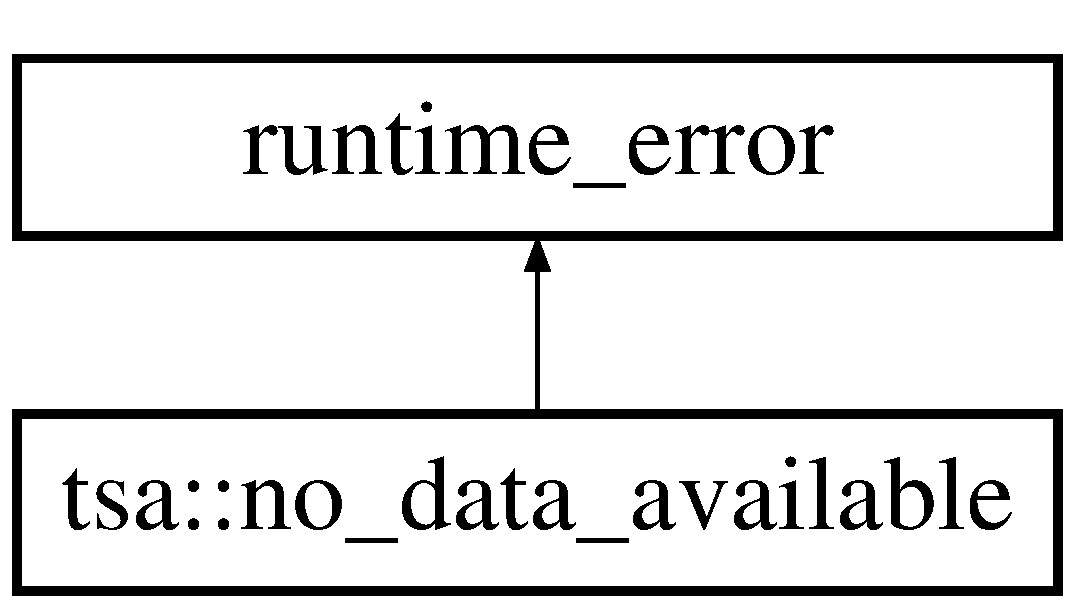
\includegraphics[height=2.000000cm]{classtsa_1_1no__data__available}
\end{center}
\end{figure}
\subsection*{Public Member Functions}
\begin{DoxyCompactItemize}
\item 
\hyperlink{classtsa_1_1no__data__available_aae9e61590d1ca7174180eb4b5c190930}{no\+\_\+data\+\_\+available} (const std\+::string \&msg)
\end{DoxyCompactItemize}


\subsection{Detailed Description}
This exception should be used when some processed data cannot be returned 

Definition at line 122 of file Algo\+Exceptions.\+hpp.



\subsection{Constructor \& Destructor Documentation}
\mbox{\Hypertarget{classtsa_1_1no__data__available_aae9e61590d1ca7174180eb4b5c190930}\label{classtsa_1_1no__data__available_aae9e61590d1ca7174180eb4b5c190930}} 
\index{tsa\+::no\+\_\+data\+\_\+available@{tsa\+::no\+\_\+data\+\_\+available}!no\+\_\+data\+\_\+available@{no\+\_\+data\+\_\+available}}
\index{no\+\_\+data\+\_\+available@{no\+\_\+data\+\_\+available}!tsa\+::no\+\_\+data\+\_\+available@{tsa\+::no\+\_\+data\+\_\+available}}
\subsubsection{\texorpdfstring{no\+\_\+data\+\_\+available()}{no\_data\_available()}}
{\footnotesize\ttfamily tsa\+::no\+\_\+data\+\_\+available\+::no\+\_\+data\+\_\+available (\begin{DoxyParamCaption}\item[{const std\+::string \&}]{msg }\end{DoxyParamCaption})\hspace{0.3cm}{\ttfamily [inline]}}

Constructor


\begin{DoxyParams}{Parameters}
{\em msg} & error message \\
\hline
\end{DoxyParams}


Definition at line 130 of file Algo\+Exceptions.\+hpp.



The documentation for this class was generated from the following file\+:\begin{DoxyCompactItemize}
\item 
/home/filip/\+Ph\+D/\+W\+D\+F\+Pipe\+\_\+test/p4\+T\+S\+A/include/\hyperlink{_algo_exceptions_8hpp}{Algo\+Exceptions.\+hpp}\end{DoxyCompactItemize}

\hypertarget{classeternity_1_1node}{}\section{eternity\+:\+:node Class Reference}
\label{classeternity_1_1node}\index{eternity\+::node@{eternity\+::node}}


{\ttfamily \#include $<$xmlscanner.\+hpp$>$}

\subsection*{Public Member Functions}
\begin{DoxyCompactItemize}
\item 
void \hyperlink{classeternity_1_1node_a05e3159af39079b860ecb1f79d436bb1}{dump} (size\+\_\+t indent)
\item 
void \hyperlink{classeternity_1_1node_a35b42655fbf388f225c108f10bf46028}{intent} (size\+\_\+t pos)
\item 
void \hyperlink{classeternity_1_1node_acab0e3d272545fa2f535d11416119eaf}{done} ()
\item 
\hyperlink{classeternity_1_1node}{node} $\ast$ \hyperlink{classeternity_1_1node_a17c2bb4c6bb9594076e91935bd970224}{found\+Child} (std\+::string tag\+Name, size\+\_\+t pos)
\item 
\hyperlink{classeternity_1_1node_a8aab11da45324aff3018c80a3b489e47}{node} ()
\item 
\hyperlink{classeternity_1_1node_ad95115f371bc4d91338735dd1c168b77}{node} (std\+::string \+\_\+name)
\item 
\hyperlink{classeternity_1_1node_aee2ebc23f893fed356c9c4c123842283}{node} (\hyperlink{classeternity_1_1node}{node} $\ast$parentnode)
\item 
virtual \hyperlink{classeternity_1_1node_a068bb1cebdb8ce5682040fe3ada60718}{$\sim$node} ()
\end{DoxyCompactItemize}
\subsection*{Public Attributes}
\begin{DoxyCompactItemize}
\item 
std\+::string \hyperlink{classeternity_1_1node_aa58fec317429adb430f6d38b3660b69a}{name}
\item 
std\+::map$<$ std\+::string, std\+::string $>$ \hyperlink{classeternity_1_1node_af12d6ec498fd30def4c6b4f21fa181c7}{attributes}
\item 
std\+::string \hyperlink{classeternity_1_1node_a8daefdb6d1fffd05b08a2f8e07c9ffb4}{value}
\item 
std\+::vector$<$ \hyperlink{classeternity_1_1node}{node} $\ast$ $>$ \hyperlink{classeternity_1_1node_ac1d7dfa57dd7ad2c13f0d6e0594d7e7f}{childs}
\item 
\hyperlink{classeternity_1_1node}{node} $\ast$ \hyperlink{classeternity_1_1node_a11a3dc9c5a20a7cae619e7bf69e09131}{parent}
\end{DoxyCompactItemize}


\subsection{Detailed Description}


Definition at line 37 of file xmlscanner.\+hpp.



\subsection{Constructor \& Destructor Documentation}
\mbox{\Hypertarget{classeternity_1_1node_a8aab11da45324aff3018c80a3b489e47}\label{classeternity_1_1node_a8aab11da45324aff3018c80a3b489e47}} 
\index{eternity\+::node@{eternity\+::node}!node@{node}}
\index{node@{node}!eternity\+::node@{eternity\+::node}}
\subsubsection{\texorpdfstring{node()}{node()}\hspace{0.1cm}{\footnotesize\ttfamily [1/3]}}
{\footnotesize\ttfamily eternity\+::node\+::node (\begin{DoxyParamCaption}{ }\end{DoxyParamCaption})}



Definition at line 34 of file xmlscanner.\+cpp.

\mbox{\Hypertarget{classeternity_1_1node_ad95115f371bc4d91338735dd1c168b77}\label{classeternity_1_1node_ad95115f371bc4d91338735dd1c168b77}} 
\index{eternity\+::node@{eternity\+::node}!node@{node}}
\index{node@{node}!eternity\+::node@{eternity\+::node}}
\subsubsection{\texorpdfstring{node()}{node()}\hspace{0.1cm}{\footnotesize\ttfamily [2/3]}}
{\footnotesize\ttfamily eternity\+::node\+::node (\begin{DoxyParamCaption}\item[{std\+::string}]{\+\_\+name }\end{DoxyParamCaption})}



Definition at line 37 of file xmlscanner.\+cpp.

\mbox{\Hypertarget{classeternity_1_1node_aee2ebc23f893fed356c9c4c123842283}\label{classeternity_1_1node_aee2ebc23f893fed356c9c4c123842283}} 
\index{eternity\+::node@{eternity\+::node}!node@{node}}
\index{node@{node}!eternity\+::node@{eternity\+::node}}
\subsubsection{\texorpdfstring{node()}{node()}\hspace{0.1cm}{\footnotesize\ttfamily [3/3]}}
{\footnotesize\ttfamily eternity\+::node\+::node (\begin{DoxyParamCaption}\item[{\hyperlink{classeternity_1_1node}{node} $\ast$}]{parentnode }\end{DoxyParamCaption})}



Definition at line 40 of file xmlscanner.\+cpp.

\mbox{\Hypertarget{classeternity_1_1node_a068bb1cebdb8ce5682040fe3ada60718}\label{classeternity_1_1node_a068bb1cebdb8ce5682040fe3ada60718}} 
\index{eternity\+::node@{eternity\+::node}!````~node@{$\sim$node}}
\index{````~node@{$\sim$node}!eternity\+::node@{eternity\+::node}}
\subsubsection{\texorpdfstring{$\sim$node()}{~node()}}
{\footnotesize\ttfamily eternity\+::node\+::$\sim$node (\begin{DoxyParamCaption}{ }\end{DoxyParamCaption})\hspace{0.3cm}{\ttfamily [virtual]}}



Definition at line 45 of file xmlscanner.\+cpp.



\subsection{Member Function Documentation}
\mbox{\Hypertarget{classeternity_1_1node_acab0e3d272545fa2f535d11416119eaf}\label{classeternity_1_1node_acab0e3d272545fa2f535d11416119eaf}} 
\index{eternity\+::node@{eternity\+::node}!done@{done}}
\index{done@{done}!eternity\+::node@{eternity\+::node}}
\subsubsection{\texorpdfstring{done()}{done()}}
{\footnotesize\ttfamily void eternity\+::node\+::done (\begin{DoxyParamCaption}{ }\end{DoxyParamCaption})}



Definition at line 69 of file xmlscanner.\+cpp.

\mbox{\Hypertarget{classeternity_1_1node_a05e3159af39079b860ecb1f79d436bb1}\label{classeternity_1_1node_a05e3159af39079b860ecb1f79d436bb1}} 
\index{eternity\+::node@{eternity\+::node}!dump@{dump}}
\index{dump@{dump}!eternity\+::node@{eternity\+::node}}
\subsubsection{\texorpdfstring{dump()}{dump()}}
{\footnotesize\ttfamily void eternity\+::node\+::dump (\begin{DoxyParamCaption}\item[{size\+\_\+t}]{indent }\end{DoxyParamCaption})}



Definition at line 49 of file xmlscanner.\+cpp.

\mbox{\Hypertarget{classeternity_1_1node_a17c2bb4c6bb9594076e91935bd970224}\label{classeternity_1_1node_a17c2bb4c6bb9594076e91935bd970224}} 
\index{eternity\+::node@{eternity\+::node}!found\+Child@{found\+Child}}
\index{found\+Child@{found\+Child}!eternity\+::node@{eternity\+::node}}
\subsubsection{\texorpdfstring{found\+Child()}{foundChild()}}
{\footnotesize\ttfamily \hyperlink{classeternity_1_1node}{node} $\ast$ eternity\+::node\+::found\+Child (\begin{DoxyParamCaption}\item[{std\+::string}]{tag\+Name,  }\item[{size\+\_\+t}]{pos }\end{DoxyParamCaption})}



Definition at line 77 of file xmlscanner.\+cpp.

\mbox{\Hypertarget{classeternity_1_1node_a35b42655fbf388f225c108f10bf46028}\label{classeternity_1_1node_a35b42655fbf388f225c108f10bf46028}} 
\index{eternity\+::node@{eternity\+::node}!intent@{intent}}
\index{intent@{intent}!eternity\+::node@{eternity\+::node}}
\subsubsection{\texorpdfstring{intent()}{intent()}}
{\footnotesize\ttfamily void eternity\+::node\+::intent (\begin{DoxyParamCaption}\item[{size\+\_\+t}]{pos }\end{DoxyParamCaption})}



Definition at line 65 of file xmlscanner.\+cpp.



\subsection{Member Data Documentation}
\mbox{\Hypertarget{classeternity_1_1node_af12d6ec498fd30def4c6b4f21fa181c7}\label{classeternity_1_1node_af12d6ec498fd30def4c6b4f21fa181c7}} 
\index{eternity\+::node@{eternity\+::node}!attributes@{attributes}}
\index{attributes@{attributes}!eternity\+::node@{eternity\+::node}}
\subsubsection{\texorpdfstring{attributes}{attributes}}
{\footnotesize\ttfamily std\+::map$<$std\+::string, std\+::string$>$ eternity\+::node\+::attributes}



Definition at line 40 of file xmlscanner.\+hpp.

\mbox{\Hypertarget{classeternity_1_1node_ac1d7dfa57dd7ad2c13f0d6e0594d7e7f}\label{classeternity_1_1node_ac1d7dfa57dd7ad2c13f0d6e0594d7e7f}} 
\index{eternity\+::node@{eternity\+::node}!childs@{childs}}
\index{childs@{childs}!eternity\+::node@{eternity\+::node}}
\subsubsection{\texorpdfstring{childs}{childs}}
{\footnotesize\ttfamily std\+::vector$<$\hyperlink{classeternity_1_1node}{node}$\ast$$>$ eternity\+::node\+::childs}



Definition at line 43 of file xmlscanner.\+hpp.

\mbox{\Hypertarget{classeternity_1_1node_aa58fec317429adb430f6d38b3660b69a}\label{classeternity_1_1node_aa58fec317429adb430f6d38b3660b69a}} 
\index{eternity\+::node@{eternity\+::node}!name@{name}}
\index{name@{name}!eternity\+::node@{eternity\+::node}}
\subsubsection{\texorpdfstring{name}{name}}
{\footnotesize\ttfamily std\+::string eternity\+::node\+::name}



Definition at line 39 of file xmlscanner.\+hpp.

\mbox{\Hypertarget{classeternity_1_1node_a11a3dc9c5a20a7cae619e7bf69e09131}\label{classeternity_1_1node_a11a3dc9c5a20a7cae619e7bf69e09131}} 
\index{eternity\+::node@{eternity\+::node}!parent@{parent}}
\index{parent@{parent}!eternity\+::node@{eternity\+::node}}
\subsubsection{\texorpdfstring{parent}{parent}}
{\footnotesize\ttfamily \hyperlink{classeternity_1_1node}{node}$\ast$ eternity\+::node\+::parent}



Definition at line 44 of file xmlscanner.\+hpp.

\mbox{\Hypertarget{classeternity_1_1node_a8daefdb6d1fffd05b08a2f8e07c9ffb4}\label{classeternity_1_1node_a8daefdb6d1fffd05b08a2f8e07c9ffb4}} 
\index{eternity\+::node@{eternity\+::node}!value@{value}}
\index{value@{value}!eternity\+::node@{eternity\+::node}}
\subsubsection{\texorpdfstring{value}{value}}
{\footnotesize\ttfamily std\+::string eternity\+::node\+::value}



Definition at line 42 of file xmlscanner.\+hpp.



The documentation for this class was generated from the following files\+:\begin{DoxyCompactItemize}
\item 
/home/filip/\+Ph\+D/\+W\+D\+F\+Pipe\+\_\+test/p4\+T\+S\+A/include/eternity/\hyperlink{xmlscanner_8hpp}{xmlscanner.\+hpp}\item 
/home/filip/\+Ph\+D/\+W\+D\+F\+Pipe\+\_\+test/p4\+T\+S\+A/include/eternity/\hyperlink{xmlscanner_8cpp}{xmlscanner.\+cpp}\end{DoxyCompactItemize}

\hypertarget{classtsa_1_1_notch_widrow}{}\section{tsa\+:\+:Notch\+Widrow Class Reference}
\label{classtsa_1_1_notch_widrow}\index{tsa\+::\+Notch\+Widrow@{tsa\+::\+Notch\+Widrow}}


Implement the lines removal using adaptive notch filters, with the Least Mean Squared method, Widrow\textquotesingle{}s like.  




{\ttfamily \#include $<$Notch\+Widrow.\+hpp$>$}

Inheritance diagram for tsa\+:\+:Notch\+Widrow\+:\begin{figure}[H]
\begin{center}
\leavevmode
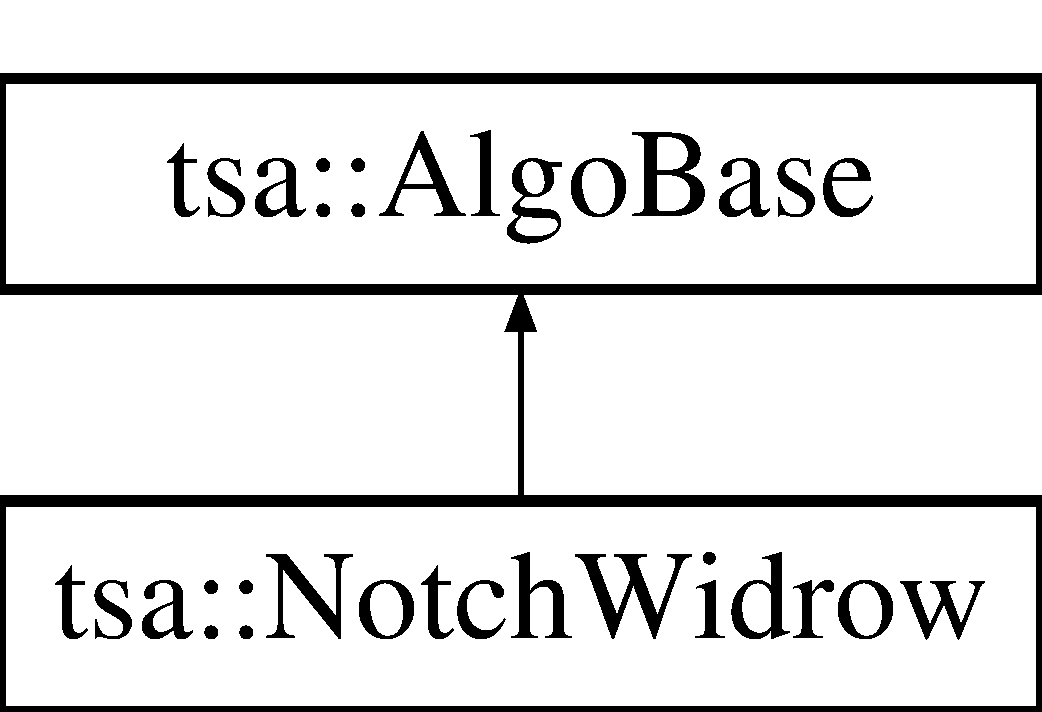
\includegraphics[height=2.000000cm]{classtsa_1_1_notch_widrow}
\end{center}
\end{figure}
\subsection*{Public Member Functions}
\begin{DoxyCompactItemize}
\item 
\hyperlink{classtsa_1_1_notch_widrow_a7e25ed1b1078586eeba5042708604f3c}{Notch\+Widrow} (unsigned int channels, \hyperlink{namespacetsa_ad260cd21c1891c4ed391fe788569aba4}{Dmatrix} \&Frequency\+List, double C=1.\+0)
\item 
\hyperlink{classtsa_1_1_notch_widrow_a035983c44683b3cebc0cc658625766f8}{Notch\+Widrow} (const \hyperlink{classtsa_1_1_notch_widrow}{Notch\+Widrow} \&from)
\item 
virtual \hyperlink{classtsa_1_1_notch_widrow_a6001ad30b1394347df1be5d9a77a46de}{$\sim$\+Notch\+Widrow} ()
\item 
void \hyperlink{classtsa_1_1_notch_widrow_af11452f632cdcb6587b6e38902739418}{operator()} (\hyperlink{namespacetsa_ac599574bcc094eda25613724b8f3ca9e}{Seq\+View\+Double} \&Input\+Data, \hyperlink{namespacetsa_ac599574bcc094eda25613724b8f3ca9e}{Seq\+View\+Double} \&Cleaned\+Data)
\item 
void \hyperlink{classtsa_1_1_notch_widrow_a1a5e3856299c5c1ee5f395dcf3a84b45}{operator()} (\hyperlink{namespacetsa_ac599574bcc094eda25613724b8f3ca9e}{Seq\+View\+Double} \&Input\+Data, \hyperlink{namespacetsa_ac599574bcc094eda25613724b8f3ca9e}{Seq\+View\+Double} \&Cleaned\+Data, \hyperlink{namespacetsa_ac599574bcc094eda25613724b8f3ca9e}{Seq\+View\+Double} \&Reference\+Signal)
\item 
\hyperlink{classtsa_1_1_notch_widrow}{Notch\+Widrow} \& \hyperlink{classtsa_1_1_notch_widrow_a5742384848310dde0e8cc5ffc8a59b22}{operator=} (const \hyperlink{classtsa_1_1_notch_widrow}{Notch\+Widrow} \&from)
\end{DoxyCompactItemize}
\begin{Indent}\textbf{ Operations}\par
\begin{DoxyCompactItemize}
\item 
void \hyperlink{classtsa_1_1_notch_widrow_a40d73f3abe99c4e73d392f68317298c7}{execute} (\hyperlink{namespacetsa_ad260cd21c1891c4ed391fe788569aba4}{Dmatrix} \&Input, \hyperlink{namespacetsa_ad260cd21c1891c4ed391fe788569aba4}{Dmatrix} \&Output)
\end{DoxyCompactItemize}
\end{Indent}
\begin{Indent}\textbf{ Getters}\par
\begin{DoxyCompactItemize}
\item 
double \hyperlink{classtsa_1_1_notch_widrow_a036b5be767039465601378f76a4f013d}{Getlstart} ()
\end{DoxyCompactItemize}
\end{Indent}
\subsection*{Private Attributes}
\begin{DoxyCompactItemize}
\item 
\hyperlink{namespacetsa_ad260cd21c1891c4ed391fe788569aba4}{Dmatrix} \hyperlink{classtsa_1_1_notch_widrow_a391286f42ba0dbede784bc90446833e4}{m\+Frequency\+List}
\item 
\hyperlink{namespacetsa_ad260cd21c1891c4ed391fe788569aba4}{Dmatrix} \hyperlink{classtsa_1_1_notch_widrow_a73d8df3ec7105a4f481edc807123df5c}{m\+Weight1}
\item 
\hyperlink{namespacetsa_ad260cd21c1891c4ed391fe788569aba4}{Dmatrix} \hyperlink{classtsa_1_1_notch_widrow_a942bc010a02f09c124589a5f467b9100}{m\+Weight2}
\item 
\hyperlink{namespacetsa_a8900fb03d849baf447a1a0efe2561fb2}{Dvector} \hyperlink{classtsa_1_1_notch_widrow_af4771f4a7d4b59bb804ee77679e13284}{m\+X1}
\item 
\hyperlink{namespacetsa_a8900fb03d849baf447a1a0efe2561fb2}{Dvector} \hyperlink{classtsa_1_1_notch_widrow_adde0e4f47ee24c548101b61e864da073}{m\+X2}
\item 
\hyperlink{namespacetsa_a8900fb03d849baf447a1a0efe2561fb2}{Dvector} \hyperlink{classtsa_1_1_notch_widrow_afa8a7585ecbd88d110ab096e344d2c0c}{m\+Cs}
\item 
\hyperlink{namespacetsa_a8900fb03d849baf447a1a0efe2561fb2}{Dvector} \hyperlink{classtsa_1_1_notch_widrow_a7b4784ec034908142ed52fa9fe33363c}{m\+Sn}
\item 
double \hyperlink{classtsa_1_1_notch_widrow_a16272fe55b1ddf22dcc04e7db1e92397}{mlstart}
\item 
\hyperlink{namespacetsa_ad260cd21c1891c4ed391fe788569aba4}{Dmatrix} \hyperlink{classtsa_1_1_notch_widrow_a11653cedb6210434d45a8f30e1dc37b8}{m\+Ref\+Sign}
\item 
double \hyperlink{classtsa_1_1_notch_widrow_acbc33d87e8a0dd156dacf5bfe40ff493}{m\+Amp}
\end{DoxyCompactItemize}


\subsection{Detailed Description}
Implement the lines removal using adaptive notch filters, with the Least Mean Squared method, Widrow\textquotesingle{}s like. 

Definition at line 71 of file Notch\+Widrow.\+hpp.



\subsection{Constructor \& Destructor Documentation}
\mbox{\Hypertarget{classtsa_1_1_notch_widrow_a7e25ed1b1078586eeba5042708604f3c}\label{classtsa_1_1_notch_widrow_a7e25ed1b1078586eeba5042708604f3c}} 
\index{tsa\+::\+Notch\+Widrow@{tsa\+::\+Notch\+Widrow}!Notch\+Widrow@{Notch\+Widrow}}
\index{Notch\+Widrow@{Notch\+Widrow}!tsa\+::\+Notch\+Widrow@{tsa\+::\+Notch\+Widrow}}
\subsubsection{\texorpdfstring{Notch\+Widrow()}{NotchWidrow()}\hspace{0.1cm}{\footnotesize\ttfamily [1/2]}}
{\footnotesize\ttfamily tsa\+::\+Notch\+Widrow\+::\+Notch\+Widrow (\begin{DoxyParamCaption}\item[{unsigned int}]{channels,  }\item[{\hyperlink{namespacetsa_ad260cd21c1891c4ed391fe788569aba4}{Dmatrix} \&}]{Frequency\+List,  }\item[{double}]{C = {\ttfamily 1.0} }\end{DoxyParamCaption})}

Constructor 
\begin{DoxyParams}{Parameters}
{\em Frequency\+List} & is a matrix containing the list of frequency to be removed. \\
\hline
\end{DoxyParams}


Definition at line 19 of file Notch\+Widrow.\+cpp.

\mbox{\Hypertarget{classtsa_1_1_notch_widrow_a035983c44683b3cebc0cc658625766f8}\label{classtsa_1_1_notch_widrow_a035983c44683b3cebc0cc658625766f8}} 
\index{tsa\+::\+Notch\+Widrow@{tsa\+::\+Notch\+Widrow}!Notch\+Widrow@{Notch\+Widrow}}
\index{Notch\+Widrow@{Notch\+Widrow}!tsa\+::\+Notch\+Widrow@{tsa\+::\+Notch\+Widrow}}
\subsubsection{\texorpdfstring{Notch\+Widrow()}{NotchWidrow()}\hspace{0.1cm}{\footnotesize\ttfamily [2/2]}}
{\footnotesize\ttfamily tsa\+::\+Notch\+Widrow\+::\+Notch\+Widrow (\begin{DoxyParamCaption}\item[{const \hyperlink{classtsa_1_1_notch_widrow}{Notch\+Widrow} \&}]{from }\end{DoxyParamCaption})}

Copy constructor


\begin{DoxyParams}{Parameters}
{\em from} & The instance that must be copied \\
\hline
\end{DoxyParams}


Definition at line 119 of file Notch\+Widrow.\+cpp.

\mbox{\Hypertarget{classtsa_1_1_notch_widrow_a6001ad30b1394347df1be5d9a77a46de}\label{classtsa_1_1_notch_widrow_a6001ad30b1394347df1be5d9a77a46de}} 
\index{tsa\+::\+Notch\+Widrow@{tsa\+::\+Notch\+Widrow}!````~Notch\+Widrow@{$\sim$\+Notch\+Widrow}}
\index{````~Notch\+Widrow@{$\sim$\+Notch\+Widrow}!tsa\+::\+Notch\+Widrow@{tsa\+::\+Notch\+Widrow}}
\subsubsection{\texorpdfstring{$\sim$\+Notch\+Widrow()}{~NotchWidrow()}}
{\footnotesize\ttfamily tsa\+::\+Notch\+Widrow\+::$\sim$\+Notch\+Widrow (\begin{DoxyParamCaption}{ }\end{DoxyParamCaption})\hspace{0.3cm}{\ttfamily [virtual]}}

Destructor 

Definition at line 32 of file Notch\+Widrow.\+cpp.



\subsection{Member Function Documentation}
\mbox{\Hypertarget{classtsa_1_1_notch_widrow_a40d73f3abe99c4e73d392f68317298c7}\label{classtsa_1_1_notch_widrow_a40d73f3abe99c4e73d392f68317298c7}} 
\index{tsa\+::\+Notch\+Widrow@{tsa\+::\+Notch\+Widrow}!execute@{execute}}
\index{execute@{execute}!tsa\+::\+Notch\+Widrow@{tsa\+::\+Notch\+Widrow}}
\subsubsection{\texorpdfstring{execute()}{execute()}}
{\footnotesize\ttfamily void tsa\+::\+Notch\+Widrow\+::execute (\begin{DoxyParamCaption}\item[{\hyperlink{namespacetsa_ad260cd21c1891c4ed391fe788569aba4}{Dmatrix} \&}]{Input,  }\item[{\hyperlink{namespacetsa_ad260cd21c1891c4ed391fe788569aba4}{Dmatrix} \&}]{Output }\end{DoxyParamCaption})}

\begin{DoxyPrecond}{Precondition}
The starting frequency list and its parameters must be given
\end{DoxyPrecond}

\begin{DoxyParams}{Parameters}
{\em Input} & Input Sequence of Data\\
\hline
{\em Output} & the cleaned sequence of data, with lines removed\\
\hline
\end{DoxyParams}
Declaration of execute operation 

Definition at line 73 of file Notch\+Widrow.\+cpp.

\mbox{\Hypertarget{classtsa_1_1_notch_widrow_a036b5be767039465601378f76a4f013d}\label{classtsa_1_1_notch_widrow_a036b5be767039465601378f76a4f013d}} 
\index{tsa\+::\+Notch\+Widrow@{tsa\+::\+Notch\+Widrow}!Getlstart@{Getlstart}}
\index{Getlstart@{Getlstart}!tsa\+::\+Notch\+Widrow@{tsa\+::\+Notch\+Widrow}}
\subsubsection{\texorpdfstring{Getlstart()}{Getlstart()}}
{\footnotesize\ttfamily double tsa\+::\+Notch\+Widrow\+::\+Getlstart (\begin{DoxyParamCaption}{ }\end{DoxyParamCaption})\hspace{0.3cm}{\ttfamily [inline]}}



Definition at line 141 of file Notch\+Widrow.\+hpp.

\mbox{\Hypertarget{classtsa_1_1_notch_widrow_af11452f632cdcb6587b6e38902739418}\label{classtsa_1_1_notch_widrow_af11452f632cdcb6587b6e38902739418}} 
\index{tsa\+::\+Notch\+Widrow@{tsa\+::\+Notch\+Widrow}!operator()@{operator()}}
\index{operator()@{operator()}!tsa\+::\+Notch\+Widrow@{tsa\+::\+Notch\+Widrow}}
\subsubsection{\texorpdfstring{operator()()}{operator()()}\hspace{0.1cm}{\footnotesize\ttfamily [1/2]}}
{\footnotesize\ttfamily void tsa\+::\+Notch\+Widrow\+::operator() (\begin{DoxyParamCaption}\item[{\hyperlink{namespacetsa_ac599574bcc094eda25613724b8f3ca9e}{Seq\+View\+Double} \&}]{Input\+Data,  }\item[{\hyperlink{namespacetsa_ac599574bcc094eda25613724b8f3ca9e}{Seq\+View\+Double} \&}]{Cleaned\+Data }\end{DoxyParamCaption})}


\begin{DoxyParams}{Parameters}
{\em Input\+Data} & \\
\hline
{\em Cleaned\+Data} & \\
\hline
\end{DoxyParams}


Definition at line 35 of file Notch\+Widrow.\+cpp.

\mbox{\Hypertarget{classtsa_1_1_notch_widrow_a1a5e3856299c5c1ee5f395dcf3a84b45}\label{classtsa_1_1_notch_widrow_a1a5e3856299c5c1ee5f395dcf3a84b45}} 
\index{tsa\+::\+Notch\+Widrow@{tsa\+::\+Notch\+Widrow}!operator()@{operator()}}
\index{operator()@{operator()}!tsa\+::\+Notch\+Widrow@{tsa\+::\+Notch\+Widrow}}
\subsubsection{\texorpdfstring{operator()()}{operator()()}\hspace{0.1cm}{\footnotesize\ttfamily [2/2]}}
{\footnotesize\ttfamily void tsa\+::\+Notch\+Widrow\+::operator() (\begin{DoxyParamCaption}\item[{\hyperlink{namespacetsa_ac599574bcc094eda25613724b8f3ca9e}{Seq\+View\+Double} \&}]{Input\+Data,  }\item[{\hyperlink{namespacetsa_ac599574bcc094eda25613724b8f3ca9e}{Seq\+View\+Double} \&}]{Cleaned\+Data,  }\item[{\hyperlink{namespacetsa_ac599574bcc094eda25613724b8f3ca9e}{Seq\+View\+Double} \&}]{Reference\+Signal }\end{DoxyParamCaption})}


\begin{DoxyParams}{Parameters}
{\em Input\+Data} & \\
\hline
{\em Cleaned\+Data} & \\
\hline
{\em Reference\+Signal} & \\
\hline
\end{DoxyParams}


Definition at line 50 of file Notch\+Widrow.\+cpp.

\mbox{\Hypertarget{classtsa_1_1_notch_widrow_a5742384848310dde0e8cc5ffc8a59b22}\label{classtsa_1_1_notch_widrow_a5742384848310dde0e8cc5ffc8a59b22}} 
\index{tsa\+::\+Notch\+Widrow@{tsa\+::\+Notch\+Widrow}!operator=@{operator=}}
\index{operator=@{operator=}!tsa\+::\+Notch\+Widrow@{tsa\+::\+Notch\+Widrow}}
\subsubsection{\texorpdfstring{operator=()}{operator=()}}
{\footnotesize\ttfamily \hyperlink{classtsa_1_1_notch_widrow}{Notch\+Widrow} \& tsa\+::\+Notch\+Widrow\+::operator= (\begin{DoxyParamCaption}\item[{const \hyperlink{classtsa_1_1_notch_widrow}{Notch\+Widrow} \&}]{from }\end{DoxyParamCaption})}

Assignement operator


\begin{DoxyParams}{Parameters}
{\em from} & The instance to be assigned from\\
\hline
\end{DoxyParams}
\begin{DoxyReturn}{Returns}
a reference to a new object 
\end{DoxyReturn}


Definition at line 130 of file Notch\+Widrow.\+cpp.



\subsection{Member Data Documentation}
\mbox{\Hypertarget{classtsa_1_1_notch_widrow_acbc33d87e8a0dd156dacf5bfe40ff493}\label{classtsa_1_1_notch_widrow_acbc33d87e8a0dd156dacf5bfe40ff493}} 
\index{tsa\+::\+Notch\+Widrow@{tsa\+::\+Notch\+Widrow}!m\+Amp@{m\+Amp}}
\index{m\+Amp@{m\+Amp}!tsa\+::\+Notch\+Widrow@{tsa\+::\+Notch\+Widrow}}
\subsubsection{\texorpdfstring{m\+Amp}{mAmp}}
{\footnotesize\ttfamily double tsa\+::\+Notch\+Widrow\+::m\+Amp\hspace{0.3cm}{\ttfamily [private]}}



Definition at line 168 of file Notch\+Widrow.\+hpp.

\mbox{\Hypertarget{classtsa_1_1_notch_widrow_afa8a7585ecbd88d110ab096e344d2c0c}\label{classtsa_1_1_notch_widrow_afa8a7585ecbd88d110ab096e344d2c0c}} 
\index{tsa\+::\+Notch\+Widrow@{tsa\+::\+Notch\+Widrow}!m\+Cs@{m\+Cs}}
\index{m\+Cs@{m\+Cs}!tsa\+::\+Notch\+Widrow@{tsa\+::\+Notch\+Widrow}}
\subsubsection{\texorpdfstring{m\+Cs}{mCs}}
{\footnotesize\ttfamily \hyperlink{namespacetsa_a8900fb03d849baf447a1a0efe2561fb2}{Dvector} tsa\+::\+Notch\+Widrow\+::m\+Cs\hspace{0.3cm}{\ttfamily [private]}}



Definition at line 164 of file Notch\+Widrow.\+hpp.

\mbox{\Hypertarget{classtsa_1_1_notch_widrow_a391286f42ba0dbede784bc90446833e4}\label{classtsa_1_1_notch_widrow_a391286f42ba0dbede784bc90446833e4}} 
\index{tsa\+::\+Notch\+Widrow@{tsa\+::\+Notch\+Widrow}!m\+Frequency\+List@{m\+Frequency\+List}}
\index{m\+Frequency\+List@{m\+Frequency\+List}!tsa\+::\+Notch\+Widrow@{tsa\+::\+Notch\+Widrow}}
\subsubsection{\texorpdfstring{m\+Frequency\+List}{mFrequencyList}}
{\footnotesize\ttfamily \hyperlink{namespacetsa_ad260cd21c1891c4ed391fe788569aba4}{Dmatrix} tsa\+::\+Notch\+Widrow\+::m\+Frequency\+List\hspace{0.3cm}{\ttfamily [private]}}



Definition at line 159 of file Notch\+Widrow.\+hpp.

\mbox{\Hypertarget{classtsa_1_1_notch_widrow_a16272fe55b1ddf22dcc04e7db1e92397}\label{classtsa_1_1_notch_widrow_a16272fe55b1ddf22dcc04e7db1e92397}} 
\index{tsa\+::\+Notch\+Widrow@{tsa\+::\+Notch\+Widrow}!mlstart@{mlstart}}
\index{mlstart@{mlstart}!tsa\+::\+Notch\+Widrow@{tsa\+::\+Notch\+Widrow}}
\subsubsection{\texorpdfstring{mlstart}{mlstart}}
{\footnotesize\ttfamily double tsa\+::\+Notch\+Widrow\+::mlstart\hspace{0.3cm}{\ttfamily [private]}}



Definition at line 166 of file Notch\+Widrow.\+hpp.

\mbox{\Hypertarget{classtsa_1_1_notch_widrow_a11653cedb6210434d45a8f30e1dc37b8}\label{classtsa_1_1_notch_widrow_a11653cedb6210434d45a8f30e1dc37b8}} 
\index{tsa\+::\+Notch\+Widrow@{tsa\+::\+Notch\+Widrow}!m\+Ref\+Sign@{m\+Ref\+Sign}}
\index{m\+Ref\+Sign@{m\+Ref\+Sign}!tsa\+::\+Notch\+Widrow@{tsa\+::\+Notch\+Widrow}}
\subsubsection{\texorpdfstring{m\+Ref\+Sign}{mRefSign}}
{\footnotesize\ttfamily \hyperlink{namespacetsa_ad260cd21c1891c4ed391fe788569aba4}{Dmatrix} tsa\+::\+Notch\+Widrow\+::m\+Ref\+Sign\hspace{0.3cm}{\ttfamily [private]}}



Definition at line 167 of file Notch\+Widrow.\+hpp.

\mbox{\Hypertarget{classtsa_1_1_notch_widrow_a7b4784ec034908142ed52fa9fe33363c}\label{classtsa_1_1_notch_widrow_a7b4784ec034908142ed52fa9fe33363c}} 
\index{tsa\+::\+Notch\+Widrow@{tsa\+::\+Notch\+Widrow}!m\+Sn@{m\+Sn}}
\index{m\+Sn@{m\+Sn}!tsa\+::\+Notch\+Widrow@{tsa\+::\+Notch\+Widrow}}
\subsubsection{\texorpdfstring{m\+Sn}{mSn}}
{\footnotesize\ttfamily \hyperlink{namespacetsa_a8900fb03d849baf447a1a0efe2561fb2}{Dvector} tsa\+::\+Notch\+Widrow\+::m\+Sn\hspace{0.3cm}{\ttfamily [private]}}



Definition at line 165 of file Notch\+Widrow.\+hpp.

\mbox{\Hypertarget{classtsa_1_1_notch_widrow_a73d8df3ec7105a4f481edc807123df5c}\label{classtsa_1_1_notch_widrow_a73d8df3ec7105a4f481edc807123df5c}} 
\index{tsa\+::\+Notch\+Widrow@{tsa\+::\+Notch\+Widrow}!m\+Weight1@{m\+Weight1}}
\index{m\+Weight1@{m\+Weight1}!tsa\+::\+Notch\+Widrow@{tsa\+::\+Notch\+Widrow}}
\subsubsection{\texorpdfstring{m\+Weight1}{mWeight1}}
{\footnotesize\ttfamily \hyperlink{namespacetsa_ad260cd21c1891c4ed391fe788569aba4}{Dmatrix} tsa\+::\+Notch\+Widrow\+::m\+Weight1\hspace{0.3cm}{\ttfamily [private]}}



Definition at line 160 of file Notch\+Widrow.\+hpp.

\mbox{\Hypertarget{classtsa_1_1_notch_widrow_a942bc010a02f09c124589a5f467b9100}\label{classtsa_1_1_notch_widrow_a942bc010a02f09c124589a5f467b9100}} 
\index{tsa\+::\+Notch\+Widrow@{tsa\+::\+Notch\+Widrow}!m\+Weight2@{m\+Weight2}}
\index{m\+Weight2@{m\+Weight2}!tsa\+::\+Notch\+Widrow@{tsa\+::\+Notch\+Widrow}}
\subsubsection{\texorpdfstring{m\+Weight2}{mWeight2}}
{\footnotesize\ttfamily \hyperlink{namespacetsa_ad260cd21c1891c4ed391fe788569aba4}{Dmatrix} tsa\+::\+Notch\+Widrow\+::m\+Weight2\hspace{0.3cm}{\ttfamily [private]}}



Definition at line 161 of file Notch\+Widrow.\+hpp.

\mbox{\Hypertarget{classtsa_1_1_notch_widrow_af4771f4a7d4b59bb804ee77679e13284}\label{classtsa_1_1_notch_widrow_af4771f4a7d4b59bb804ee77679e13284}} 
\index{tsa\+::\+Notch\+Widrow@{tsa\+::\+Notch\+Widrow}!m\+X1@{m\+X1}}
\index{m\+X1@{m\+X1}!tsa\+::\+Notch\+Widrow@{tsa\+::\+Notch\+Widrow}}
\subsubsection{\texorpdfstring{m\+X1}{mX1}}
{\footnotesize\ttfamily \hyperlink{namespacetsa_a8900fb03d849baf447a1a0efe2561fb2}{Dvector} tsa\+::\+Notch\+Widrow\+::m\+X1\hspace{0.3cm}{\ttfamily [private]}}



Definition at line 162 of file Notch\+Widrow.\+hpp.

\mbox{\Hypertarget{classtsa_1_1_notch_widrow_adde0e4f47ee24c548101b61e864da073}\label{classtsa_1_1_notch_widrow_adde0e4f47ee24c548101b61e864da073}} 
\index{tsa\+::\+Notch\+Widrow@{tsa\+::\+Notch\+Widrow}!m\+X2@{m\+X2}}
\index{m\+X2@{m\+X2}!tsa\+::\+Notch\+Widrow@{tsa\+::\+Notch\+Widrow}}
\subsubsection{\texorpdfstring{m\+X2}{mX2}}
{\footnotesize\ttfamily \hyperlink{namespacetsa_a8900fb03d849baf447a1a0efe2561fb2}{Dvector} tsa\+::\+Notch\+Widrow\+::m\+X2\hspace{0.3cm}{\ttfamily [private]}}



Definition at line 163 of file Notch\+Widrow.\+hpp.



The documentation for this class was generated from the following files\+:\begin{DoxyCompactItemize}
\item 
/home/filip/\+Ph\+D/\+W\+D\+F\+Pipe\+\_\+test/p4\+T\+S\+A/include/\hyperlink{_notch_widrow_8hpp}{Notch\+Widrow.\+hpp}\item 
/home/filip/\+Ph\+D/\+W\+D\+F\+Pipe\+\_\+test/p4\+T\+S\+A/src/\hyperlink{_notch_widrow_8cpp}{Notch\+Widrow.\+cpp}\end{DoxyCompactItemize}

\hypertarget{structeternity_1_1objects}{}\section{eternity\+:\+:objects Struct Reference}
\label{structeternity_1_1objects}\index{eternity\+::objects@{eternity\+::objects}}


{\ttfamily \#include $<$algorithms.\+hpp$>$}

\subsection*{Public Member Functions}
\begin{DoxyCompactItemize}
\item 
{\footnotesize template$<$class T , class Archive $>$ }\\void \hyperlink{structeternity_1_1objects_a1c4f6adbfec429e299ed9b87d3e882dc}{xml\+\_\+write} (Archive \&\hyperlink{classeternity_1_1archive}{archive}, std\+::string key, T \&x)
\item 
{\footnotesize template$<$class Value\+Type , class Archive $>$ }\\void \hyperlink{structeternity_1_1objects_a784de99cba7a1d4a1a048fa6a4ac5a4f}{xml\+\_\+read} (Archive \&\hyperlink{classeternity_1_1archive}{archive}, std\+::string key, Value\+Type $\ast$var, size\+\_\+t pos)
\item 
{\footnotesize template$<$class T , class Archive $>$ }\\void \hyperlink{structeternity_1_1objects_a4a22aa281cdd22163b1a4f52065185e6}{write} (Archive \&\hyperlink{classeternity_1_1archive}{archive}, T \&x)
\item 
{\footnotesize template$<$class Value\+Type , class Archive $>$ }\\void \hyperlink{structeternity_1_1objects_a7454fa173d59bfe23b5ac6fa78cbdfc9}{read} (Archive \&\hyperlink{classeternity_1_1archive}{archive}, Value\+Type $\ast$var)
\end{DoxyCompactItemize}


\subsection{Detailed Description}
Manage persistence of object containers (e.\+g. collections of stack allocated objects) This struct is not intended to direct use but must be passed as template parameter of sequence struct. 

Definition at line 80 of file algorithms.\+hpp.



\subsection{Member Function Documentation}
\mbox{\Hypertarget{structeternity_1_1objects_a7454fa173d59bfe23b5ac6fa78cbdfc9}\label{structeternity_1_1objects_a7454fa173d59bfe23b5ac6fa78cbdfc9}} 
\index{eternity\+::objects@{eternity\+::objects}!read@{read}}
\index{read@{read}!eternity\+::objects@{eternity\+::objects}}
\subsubsection{\texorpdfstring{read()}{read()}}
{\footnotesize\ttfamily template$<$class Value\+Type , class Archive $>$ \\
void eternity\+::objects\+::read (\begin{DoxyParamCaption}\item[{Archive \&}]{archive,  }\item[{Value\+Type $\ast$}]{var }\end{DoxyParamCaption})}



Definition at line 110 of file algorithms.\+hpp.

\mbox{\Hypertarget{structeternity_1_1objects_a4a22aa281cdd22163b1a4f52065185e6}\label{structeternity_1_1objects_a4a22aa281cdd22163b1a4f52065185e6}} 
\index{eternity\+::objects@{eternity\+::objects}!write@{write}}
\index{write@{write}!eternity\+::objects@{eternity\+::objects}}
\subsubsection{\texorpdfstring{write()}{write()}}
{\footnotesize\ttfamily template$<$class T , class Archive $>$ \\
void eternity\+::objects\+::write (\begin{DoxyParamCaption}\item[{Archive \&}]{archive,  }\item[{T \&}]{x }\end{DoxyParamCaption})}



Definition at line 105 of file algorithms.\+hpp.

\mbox{\Hypertarget{structeternity_1_1objects_a784de99cba7a1d4a1a048fa6a4ac5a4f}\label{structeternity_1_1objects_a784de99cba7a1d4a1a048fa6a4ac5a4f}} 
\index{eternity\+::objects@{eternity\+::objects}!xml\+\_\+read@{xml\+\_\+read}}
\index{xml\+\_\+read@{xml\+\_\+read}!eternity\+::objects@{eternity\+::objects}}
\subsubsection{\texorpdfstring{xml\+\_\+read()}{xml\_read()}}
{\footnotesize\ttfamily template$<$class Value\+Type , class Archive $>$ \\
void eternity\+::objects\+::xml\+\_\+read (\begin{DoxyParamCaption}\item[{Archive \&}]{archive,  }\item[{std\+::string}]{key,  }\item[{Value\+Type $\ast$}]{var,  }\item[{size\+\_\+t}]{pos }\end{DoxyParamCaption})}



Definition at line 100 of file algorithms.\+hpp.

\mbox{\Hypertarget{structeternity_1_1objects_a1c4f6adbfec429e299ed9b87d3e882dc}\label{structeternity_1_1objects_a1c4f6adbfec429e299ed9b87d3e882dc}} 
\index{eternity\+::objects@{eternity\+::objects}!xml\+\_\+write@{xml\+\_\+write}}
\index{xml\+\_\+write@{xml\+\_\+write}!eternity\+::objects@{eternity\+::objects}}
\subsubsection{\texorpdfstring{xml\+\_\+write()}{xml\_write()}}
{\footnotesize\ttfamily template$<$class T , class Archive $>$ \\
void eternity\+::objects\+::xml\+\_\+write (\begin{DoxyParamCaption}\item[{Archive \&}]{archive,  }\item[{std\+::string}]{key,  }\item[{T \&}]{x }\end{DoxyParamCaption})}



Definition at line 95 of file algorithms.\+hpp.



The documentation for this struct was generated from the following file\+:\begin{DoxyCompactItemize}
\item 
/home/filip/\+Ph\+D/\+W\+D\+F\+Pipe\+\_\+test/p4\+T\+S\+A/include/eternity/\hyperlink{algorithms_8hpp}{algorithms.\+hpp}\end{DoxyCompactItemize}

\hypertarget{classtsa_1_1_parcor2_a_r}{}\section{tsa\+:\+:Parcor2\+AR Class Reference}
\label{classtsa_1_1_parcor2_a_r}\index{tsa\+::\+Parcor2\+AR@{tsa\+::\+Parcor2\+AR}}


Estimate the AR parameters by the Parcor.  




{\ttfamily \#include $<$Parcor2\+A\+R.\+hpp$>$}

Inheritance diagram for tsa\+:\+:Parcor2\+AR\+:\begin{figure}[H]
\begin{center}
\leavevmode
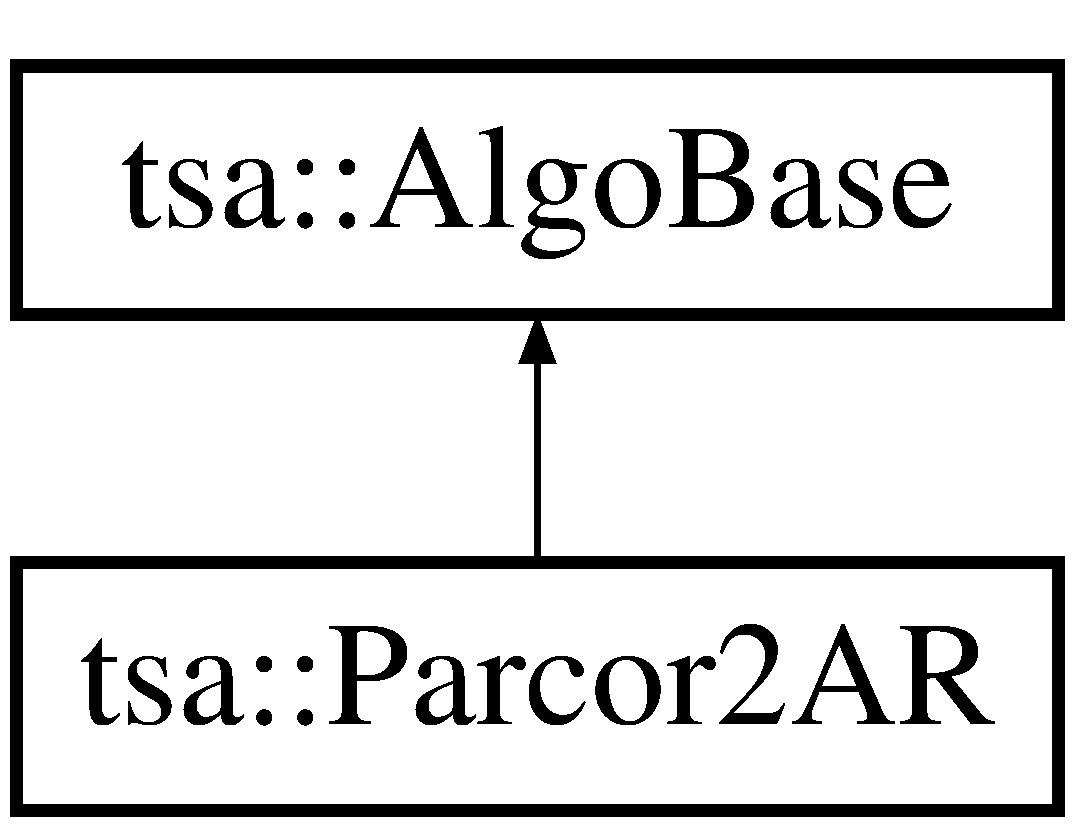
\includegraphics[height=2.000000cm]{classtsa_1_1_parcor2_a_r}
\end{center}
\end{figure}
\subsection*{Public Member Functions}
\begin{DoxyCompactItemize}
\item 
\hyperlink{classtsa_1_1_parcor2_a_r_a071a1e9ef52185df08d6889937bf4a15}{Parcor2\+AR} ()
\item 
virtual \hyperlink{classtsa_1_1_parcor2_a_r_a048e923396810067505a8a18ca95ec3a}{$\sim$\+Parcor2\+AR} ()
\item 
\hyperlink{namespacetsa_a8900fb03d849baf447a1a0efe2561fb2}{Dvector} \hyperlink{classtsa_1_1_parcor2_a_r_aa87caf6b20cdb03a33fddf7e8c9beeef}{operator()} (\hyperlink{namespacetsa_a8900fb03d849baf447a1a0efe2561fb2}{Dvector} Parcor)
\end{DoxyCompactItemize}
\begin{Indent}\textbf{ Operations}\par
\begin{DoxyCompactItemize}
\item 
void \hyperlink{classtsa_1_1_parcor2_a_r_a0a761baa7118ecfe61e612c1ae27a360}{execute} (\hyperlink{namespacetsa_a8900fb03d849baf447a1a0efe2561fb2}{Dvector} \&Parcor, \hyperlink{namespacetsa_a8900fb03d849baf447a1a0efe2561fb2}{Dvector} \&AR)
\end{DoxyCompactItemize}
\end{Indent}


\subsection{Detailed Description}
Estimate the AR parameters by the Parcor. 

Definition at line 72 of file Parcor2\+A\+R.\+hpp.



\subsection{Constructor \& Destructor Documentation}
\mbox{\Hypertarget{classtsa_1_1_parcor2_a_r_a071a1e9ef52185df08d6889937bf4a15}\label{classtsa_1_1_parcor2_a_r_a071a1e9ef52185df08d6889937bf4a15}} 
\index{tsa\+::\+Parcor2\+AR@{tsa\+::\+Parcor2\+AR}!Parcor2\+AR@{Parcor2\+AR}}
\index{Parcor2\+AR@{Parcor2\+AR}!tsa\+::\+Parcor2\+AR@{tsa\+::\+Parcor2\+AR}}
\subsubsection{\texorpdfstring{Parcor2\+A\+R()}{Parcor2AR()}}
{\footnotesize\ttfamily tsa\+::\+Parcor2\+A\+R\+::\+Parcor2\+AR (\begin{DoxyParamCaption}{ }\end{DoxyParamCaption})}

Constructor 

Definition at line 19 of file Parcor2\+A\+R.\+cpp.

\mbox{\Hypertarget{classtsa_1_1_parcor2_a_r_a048e923396810067505a8a18ca95ec3a}\label{classtsa_1_1_parcor2_a_r_a048e923396810067505a8a18ca95ec3a}} 
\index{tsa\+::\+Parcor2\+AR@{tsa\+::\+Parcor2\+AR}!````~Parcor2\+AR@{$\sim$\+Parcor2\+AR}}
\index{````~Parcor2\+AR@{$\sim$\+Parcor2\+AR}!tsa\+::\+Parcor2\+AR@{tsa\+::\+Parcor2\+AR}}
\subsubsection{\texorpdfstring{$\sim$\+Parcor2\+A\+R()}{~Parcor2AR()}}
{\footnotesize\ttfamily tsa\+::\+Parcor2\+A\+R\+::$\sim$\+Parcor2\+AR (\begin{DoxyParamCaption}{ }\end{DoxyParamCaption})\hspace{0.3cm}{\ttfamily [virtual]}}

Destructor 

Definition at line 22 of file Parcor2\+A\+R.\+cpp.



\subsection{Member Function Documentation}
\mbox{\Hypertarget{classtsa_1_1_parcor2_a_r_a0a761baa7118ecfe61e612c1ae27a360}\label{classtsa_1_1_parcor2_a_r_a0a761baa7118ecfe61e612c1ae27a360}} 
\index{tsa\+::\+Parcor2\+AR@{tsa\+::\+Parcor2\+AR}!execute@{execute}}
\index{execute@{execute}!tsa\+::\+Parcor2\+AR@{tsa\+::\+Parcor2\+AR}}
\subsubsection{\texorpdfstring{execute()}{execute()}}
{\footnotesize\ttfamily void tsa\+::\+Parcor2\+A\+R\+::execute (\begin{DoxyParamCaption}\item[{\hyperlink{namespacetsa_a8900fb03d849baf447a1a0efe2561fb2}{Dvector} \&}]{Parcor,  }\item[{\hyperlink{namespacetsa_a8900fb03d849baf447a1a0efe2561fb2}{Dvector} \&}]{AR }\end{DoxyParamCaption})}

The execute method transform the parcor in AR


\begin{DoxyParams}{Parameters}
{\em Parcor} & reflection coefficients vector \\
\hline
{\em AR} & autoregressive parameters \\
\hline
\end{DoxyParams}


Definition at line 32 of file Parcor2\+A\+R.\+cpp.

\mbox{\Hypertarget{classtsa_1_1_parcor2_a_r_aa87caf6b20cdb03a33fddf7e8c9beeef}\label{classtsa_1_1_parcor2_a_r_aa87caf6b20cdb03a33fddf7e8c9beeef}} 
\index{tsa\+::\+Parcor2\+AR@{tsa\+::\+Parcor2\+AR}!operator()@{operator()}}
\index{operator()@{operator()}!tsa\+::\+Parcor2\+AR@{tsa\+::\+Parcor2\+AR}}
\subsubsection{\texorpdfstring{operator()()}{operator()()}}
{\footnotesize\ttfamily \hyperlink{namespacetsa_a8900fb03d849baf447a1a0efe2561fb2}{Dvector} tsa\+::\+Parcor2\+A\+R\+::operator() (\begin{DoxyParamCaption}\item[{\hyperlink{namespacetsa_a8900fb03d849baf447a1a0efe2561fb2}{Dvector}}]{Parcor }\end{DoxyParamCaption})}



Definition at line 25 of file Parcor2\+A\+R.\+cpp.



The documentation for this class was generated from the following files\+:\begin{DoxyCompactItemize}
\item 
/home/filip/\+Ph\+D/\+W\+D\+F\+Pipe\+\_\+test/p4\+T\+S\+A/include/\hyperlink{_parcor2_a_r_8hpp}{Parcor2\+A\+R.\+hpp}\item 
/home/filip/\+Ph\+D/\+W\+D\+F\+Pipe\+\_\+test/p4\+T\+S\+A/src/\hyperlink{_parcor2_a_r_8cpp}{Parcor2\+A\+R.\+cpp}\end{DoxyCompactItemize}

\hypertarget{classtsa_1_1_parse_parameter_string}{}\section{tsa\+:\+:Parse\+Parameter\+String Class Reference}
\label{classtsa_1_1_parse_parameter_string}\index{tsa\+::\+Parse\+Parameter\+String@{tsa\+::\+Parse\+Parameter\+String}}


{\ttfamily \#include $<$tsa\+Utility\+Functions.\+hpp$>$}

\subsection*{Public Member Functions}
\begin{DoxyCompactItemize}
\item 
\hyperlink{classtsa_1_1_parse_parameter_string_a68e6d37bb098c062d0e4eba92847c4fe}{Parse\+Parameter\+String} (const std\+::string \&parlist)
\item 
\hyperlink{classtsa_1_1_parse_parameter_string_a67bcdd6d213f9dcc3a229a105e8ad319}{$\sim$\+Parse\+Parameter\+String} ()
\item 
double \hyperlink{classtsa_1_1_parse_parameter_string_a36f54e156537db06f4aca02194cba5cf}{Get\+Float} (int n)
\item 
int \hyperlink{classtsa_1_1_parse_parameter_string_ac4ebad66e2a7645e1c49ecb87a126003}{Get\+Int} (int n)
\item 
std\+::string \hyperlink{classtsa_1_1_parse_parameter_string_a37cb52222e539bd6a3cf56cbeec0b958}{Get\+String} (int n)
\end{DoxyCompactItemize}
\subsection*{Private Attributes}
\begin{DoxyCompactItemize}
\item 
\hyperlink{class_function_parser}{Function\+Parser} \hyperlink{classtsa_1_1_parse_parameter_string_ab2648c4056632b436348effef55e73e5}{fparser}
\item 
char $\ast$ \hyperlink{classtsa_1_1_parse_parameter_string_aa90c11badf0c45d4efc7e2dd2c912100}{m\+Par\+List}
\item 
char $\ast$ \hyperlink{classtsa_1_1_parse_parameter_string_a3632dcdadae1f3578194c9ba14d4b7c8}{m\+Tmp}
\end{DoxyCompactItemize}


\subsection{Detailed Description}


Definition at line 74 of file tsa\+Utility\+Functions.\+hpp.



\subsection{Constructor \& Destructor Documentation}
\mbox{\Hypertarget{classtsa_1_1_parse_parameter_string_a68e6d37bb098c062d0e4eba92847c4fe}\label{classtsa_1_1_parse_parameter_string_a68e6d37bb098c062d0e4eba92847c4fe}} 
\index{tsa\+::\+Parse\+Parameter\+String@{tsa\+::\+Parse\+Parameter\+String}!Parse\+Parameter\+String@{Parse\+Parameter\+String}}
\index{Parse\+Parameter\+String@{Parse\+Parameter\+String}!tsa\+::\+Parse\+Parameter\+String@{tsa\+::\+Parse\+Parameter\+String}}
\subsubsection{\texorpdfstring{Parse\+Parameter\+String()}{ParseParameterString()}}
{\footnotesize\ttfamily tsa\+::\+Parse\+Parameter\+String\+::\+Parse\+Parameter\+String (\begin{DoxyParamCaption}\item[{const std\+::string \&}]{parlist }\end{DoxyParamCaption})\hspace{0.3cm}{\ttfamily [inline]}}



Definition at line 77 of file tsa\+Utility\+Functions.\+hpp.

\mbox{\Hypertarget{classtsa_1_1_parse_parameter_string_a67bcdd6d213f9dcc3a229a105e8ad319}\label{classtsa_1_1_parse_parameter_string_a67bcdd6d213f9dcc3a229a105e8ad319}} 
\index{tsa\+::\+Parse\+Parameter\+String@{tsa\+::\+Parse\+Parameter\+String}!````~Parse\+Parameter\+String@{$\sim$\+Parse\+Parameter\+String}}
\index{````~Parse\+Parameter\+String@{$\sim$\+Parse\+Parameter\+String}!tsa\+::\+Parse\+Parameter\+String@{tsa\+::\+Parse\+Parameter\+String}}
\subsubsection{\texorpdfstring{$\sim$\+Parse\+Parameter\+String()}{~ParseParameterString()}}
{\footnotesize\ttfamily tsa\+::\+Parse\+Parameter\+String\+::$\sim$\+Parse\+Parameter\+String (\begin{DoxyParamCaption}{ }\end{DoxyParamCaption})\hspace{0.3cm}{\ttfamily [inline]}}



Definition at line 83 of file tsa\+Utility\+Functions.\+hpp.



\subsection{Member Function Documentation}
\mbox{\Hypertarget{classtsa_1_1_parse_parameter_string_a36f54e156537db06f4aca02194cba5cf}\label{classtsa_1_1_parse_parameter_string_a36f54e156537db06f4aca02194cba5cf}} 
\index{tsa\+::\+Parse\+Parameter\+String@{tsa\+::\+Parse\+Parameter\+String}!Get\+Float@{Get\+Float}}
\index{Get\+Float@{Get\+Float}!tsa\+::\+Parse\+Parameter\+String@{tsa\+::\+Parse\+Parameter\+String}}
\subsubsection{\texorpdfstring{Get\+Float()}{GetFloat()}}
{\footnotesize\ttfamily double tsa\+::\+Parse\+Parameter\+String\+::\+Get\+Float (\begin{DoxyParamCaption}\item[{int}]{n }\end{DoxyParamCaption})\hspace{0.3cm}{\ttfamily [inline]}}



Definition at line 87 of file tsa\+Utility\+Functions.\+hpp.

\mbox{\Hypertarget{classtsa_1_1_parse_parameter_string_ac4ebad66e2a7645e1c49ecb87a126003}\label{classtsa_1_1_parse_parameter_string_ac4ebad66e2a7645e1c49ecb87a126003}} 
\index{tsa\+::\+Parse\+Parameter\+String@{tsa\+::\+Parse\+Parameter\+String}!Get\+Int@{Get\+Int}}
\index{Get\+Int@{Get\+Int}!tsa\+::\+Parse\+Parameter\+String@{tsa\+::\+Parse\+Parameter\+String}}
\subsubsection{\texorpdfstring{Get\+Int()}{GetInt()}}
{\footnotesize\ttfamily int tsa\+::\+Parse\+Parameter\+String\+::\+Get\+Int (\begin{DoxyParamCaption}\item[{int}]{n }\end{DoxyParamCaption})\hspace{0.3cm}{\ttfamily [inline]}}



Definition at line 102 of file tsa\+Utility\+Functions.\+hpp.

\mbox{\Hypertarget{classtsa_1_1_parse_parameter_string_a37cb52222e539bd6a3cf56cbeec0b958}\label{classtsa_1_1_parse_parameter_string_a37cb52222e539bd6a3cf56cbeec0b958}} 
\index{tsa\+::\+Parse\+Parameter\+String@{tsa\+::\+Parse\+Parameter\+String}!Get\+String@{Get\+String}}
\index{Get\+String@{Get\+String}!tsa\+::\+Parse\+Parameter\+String@{tsa\+::\+Parse\+Parameter\+String}}
\subsubsection{\texorpdfstring{Get\+String()}{GetString()}}
{\footnotesize\ttfamily std\+::string tsa\+::\+Parse\+Parameter\+String\+::\+Get\+String (\begin{DoxyParamCaption}\item[{int}]{n }\end{DoxyParamCaption})\hspace{0.3cm}{\ttfamily [inline]}}



Definition at line 117 of file tsa\+Utility\+Functions.\+hpp.



\subsection{Member Data Documentation}
\mbox{\Hypertarget{classtsa_1_1_parse_parameter_string_ab2648c4056632b436348effef55e73e5}\label{classtsa_1_1_parse_parameter_string_ab2648c4056632b436348effef55e73e5}} 
\index{tsa\+::\+Parse\+Parameter\+String@{tsa\+::\+Parse\+Parameter\+String}!fparser@{fparser}}
\index{fparser@{fparser}!tsa\+::\+Parse\+Parameter\+String@{tsa\+::\+Parse\+Parameter\+String}}
\subsubsection{\texorpdfstring{fparser}{fparser}}
{\footnotesize\ttfamily \hyperlink{class_function_parser}{Function\+Parser} tsa\+::\+Parse\+Parameter\+String\+::fparser\hspace{0.3cm}{\ttfamily [private]}}



Definition at line 135 of file tsa\+Utility\+Functions.\+hpp.

\mbox{\Hypertarget{classtsa_1_1_parse_parameter_string_aa90c11badf0c45d4efc7e2dd2c912100}\label{classtsa_1_1_parse_parameter_string_aa90c11badf0c45d4efc7e2dd2c912100}} 
\index{tsa\+::\+Parse\+Parameter\+String@{tsa\+::\+Parse\+Parameter\+String}!m\+Par\+List@{m\+Par\+List}}
\index{m\+Par\+List@{m\+Par\+List}!tsa\+::\+Parse\+Parameter\+String@{tsa\+::\+Parse\+Parameter\+String}}
\subsubsection{\texorpdfstring{m\+Par\+List}{mParList}}
{\footnotesize\ttfamily char$\ast$ tsa\+::\+Parse\+Parameter\+String\+::m\+Par\+List\hspace{0.3cm}{\ttfamily [private]}}



Definition at line 136 of file tsa\+Utility\+Functions.\+hpp.

\mbox{\Hypertarget{classtsa_1_1_parse_parameter_string_a3632dcdadae1f3578194c9ba14d4b7c8}\label{classtsa_1_1_parse_parameter_string_a3632dcdadae1f3578194c9ba14d4b7c8}} 
\index{tsa\+::\+Parse\+Parameter\+String@{tsa\+::\+Parse\+Parameter\+String}!m\+Tmp@{m\+Tmp}}
\index{m\+Tmp@{m\+Tmp}!tsa\+::\+Parse\+Parameter\+String@{tsa\+::\+Parse\+Parameter\+String}}
\subsubsection{\texorpdfstring{m\+Tmp}{mTmp}}
{\footnotesize\ttfamily char$\ast$ tsa\+::\+Parse\+Parameter\+String\+::m\+Tmp\hspace{0.3cm}{\ttfamily [private]}}



Definition at line 137 of file tsa\+Utility\+Functions.\+hpp.



The documentation for this class was generated from the following file\+:\begin{DoxyCompactItemize}
\item 
/home/filip/\+Ph\+D/\+W\+D\+F\+Pipe\+\_\+test/p4\+T\+S\+A/include/\hyperlink{tsa_utility_functions_8hpp}{tsa\+Utility\+Functions.\+hpp}\end{DoxyCompactItemize}

\hypertarget{structeternity_1_1pointers}{}\section{eternity\+:\+:pointers Struct Reference}
\label{structeternity_1_1pointers}\index{eternity\+::pointers@{eternity\+::pointers}}


{\ttfamily \#include $<$algorithms.\+hpp$>$}

\subsection*{Public Member Functions}
\begin{DoxyCompactItemize}
\item 
{\footnotesize template$<$class T , class Archive $>$ }\\void \hyperlink{structeternity_1_1pointers_a9ac5397bcf7d4e363f80c325b86e7966}{xml\+\_\+write} (Archive \&\hyperlink{classeternity_1_1archive}{archive}, std\+::string key, T \&x)
\item 
{\footnotesize template$<$class Value\+Type , class Archive $>$ }\\void \hyperlink{structeternity_1_1pointers_a82633874b86bdf07241befe07601fa10}{xml\+\_\+read} (Archive \&\hyperlink{classeternity_1_1archive}{archive}, std\+::string key, Value\+Type $\ast$var, size\+\_\+t pos)
\item 
{\footnotesize template$<$class T , class Archive $>$ }\\void \hyperlink{structeternity_1_1pointers_a5b2f7a5240aa5f6b19b3e615886ae5a3}{write} (Archive \&\hyperlink{classeternity_1_1archive}{archive}, T \&x)
\item 
{\footnotesize template$<$class Value\+Type , class Archive $>$ }\\void \hyperlink{structeternity_1_1pointers_a393c2b0b219bf16b8fcc372aaa19f185}{read} (Archive \&\hyperlink{classeternity_1_1archive}{archive}, Value\+Type $\ast$var)
\end{DoxyCompactItemize}


\subsection{Detailed Description}
Manage persistence of object pointers containers (e.\+g. collections of heap allocated objects) This struct is not intended to direct use but must be passed as template parameter of sequence struct. 

Definition at line 118 of file algorithms.\+hpp.



\subsection{Member Function Documentation}
\mbox{\Hypertarget{structeternity_1_1pointers_a393c2b0b219bf16b8fcc372aaa19f185}\label{structeternity_1_1pointers_a393c2b0b219bf16b8fcc372aaa19f185}} 
\index{eternity\+::pointers@{eternity\+::pointers}!read@{read}}
\index{read@{read}!eternity\+::pointers@{eternity\+::pointers}}
\subsubsection{\texorpdfstring{read()}{read()}}
{\footnotesize\ttfamily template$<$class Value\+Type , class Archive $>$ \\
void eternity\+::pointers\+::read (\begin{DoxyParamCaption}\item[{Archive \&}]{archive,  }\item[{Value\+Type $\ast$}]{var }\end{DoxyParamCaption})}



Definition at line 148 of file algorithms.\+hpp.

\mbox{\Hypertarget{structeternity_1_1pointers_a5b2f7a5240aa5f6b19b3e615886ae5a3}\label{structeternity_1_1pointers_a5b2f7a5240aa5f6b19b3e615886ae5a3}} 
\index{eternity\+::pointers@{eternity\+::pointers}!write@{write}}
\index{write@{write}!eternity\+::pointers@{eternity\+::pointers}}
\subsubsection{\texorpdfstring{write()}{write()}}
{\footnotesize\ttfamily template$<$class T , class Archive $>$ \\
void eternity\+::pointers\+::write (\begin{DoxyParamCaption}\item[{Archive \&}]{archive,  }\item[{T \&}]{x }\end{DoxyParamCaption})}



Definition at line 143 of file algorithms.\+hpp.

\mbox{\Hypertarget{structeternity_1_1pointers_a82633874b86bdf07241befe07601fa10}\label{structeternity_1_1pointers_a82633874b86bdf07241befe07601fa10}} 
\index{eternity\+::pointers@{eternity\+::pointers}!xml\+\_\+read@{xml\+\_\+read}}
\index{xml\+\_\+read@{xml\+\_\+read}!eternity\+::pointers@{eternity\+::pointers}}
\subsubsection{\texorpdfstring{xml\+\_\+read()}{xml\_read()}}
{\footnotesize\ttfamily template$<$class Value\+Type , class Archive $>$ \\
void eternity\+::pointers\+::xml\+\_\+read (\begin{DoxyParamCaption}\item[{Archive \&}]{archive,  }\item[{std\+::string}]{key,  }\item[{Value\+Type $\ast$}]{var,  }\item[{size\+\_\+t}]{pos }\end{DoxyParamCaption})}



Definition at line 138 of file algorithms.\+hpp.

\mbox{\Hypertarget{structeternity_1_1pointers_a9ac5397bcf7d4e363f80c325b86e7966}\label{structeternity_1_1pointers_a9ac5397bcf7d4e363f80c325b86e7966}} 
\index{eternity\+::pointers@{eternity\+::pointers}!xml\+\_\+write@{xml\+\_\+write}}
\index{xml\+\_\+write@{xml\+\_\+write}!eternity\+::pointers@{eternity\+::pointers}}
\subsubsection{\texorpdfstring{xml\+\_\+write()}{xml\_write()}}
{\footnotesize\ttfamily template$<$class T , class Archive $>$ \\
void eternity\+::pointers\+::xml\+\_\+write (\begin{DoxyParamCaption}\item[{Archive \&}]{archive,  }\item[{std\+::string}]{key,  }\item[{T \&}]{x }\end{DoxyParamCaption})}



Definition at line 133 of file algorithms.\+hpp.



The documentation for this struct was generated from the following file\+:\begin{DoxyCompactItemize}
\item 
/home/filip/\+Ph\+D/\+W\+D\+F\+Pipe\+\_\+test/p4\+T\+S\+A/include/eternity/\hyperlink{algorithms_8hpp}{algorithms.\+hpp}\end{DoxyCompactItemize}

\hypertarget{structeternity_1_1primitives}{}\section{eternity\+:\+:primitives Struct Reference}
\label{structeternity_1_1primitives}\index{eternity\+::primitives@{eternity\+::primitives}}


{\ttfamily \#include $<$algorithms.\+hpp$>$}

\subsection*{Public Member Functions}
\begin{DoxyCompactItemize}
\item 
{\footnotesize template$<$class T , class Archive $>$ }\\void \hyperlink{structeternity_1_1primitives_af5a6a3550f36eb25ad9372989614f162}{xml\+\_\+write} (Archive \&\hyperlink{classeternity_1_1archive}{archive}, std\+::string key, T \&x)
\item 
{\footnotesize template$<$class Value\+Type , class Archive $>$ }\\void \hyperlink{structeternity_1_1primitives_af056cf9c18929b6ec47552e9cbb16b77}{xml\+\_\+read} (Archive \&\hyperlink{classeternity_1_1archive}{archive}, std\+::string key, Value\+Type $\ast$var, size\+\_\+t pos)
\item 
{\footnotesize template$<$class T , class Archive $>$ }\\void \hyperlink{structeternity_1_1primitives_ace523d3626457362731f78d6a8b3d325}{write} (Archive \&\hyperlink{classeternity_1_1archive}{archive}, T \&x)
\item 
{\footnotesize template$<$class Value\+Type , class Archive $>$ }\\void \hyperlink{structeternity_1_1primitives_a9770d350c89a97245bf15447586e40cb}{read} (Archive \&\hyperlink{classeternity_1_1archive}{archive}, Value\+Type $\ast$var)
\end{DoxyCompactItemize}


\subsection{Detailed Description}
Manage persistence of primitive containers (e.\+g. collections of int, float, double. etc.) This struct is not intended to direct use but must be passed as template parameter of sequence struct. 

Definition at line 42 of file algorithms.\+hpp.



\subsection{Member Function Documentation}
\mbox{\Hypertarget{structeternity_1_1primitives_a9770d350c89a97245bf15447586e40cb}\label{structeternity_1_1primitives_a9770d350c89a97245bf15447586e40cb}} 
\index{eternity\+::primitives@{eternity\+::primitives}!read@{read}}
\index{read@{read}!eternity\+::primitives@{eternity\+::primitives}}
\subsubsection{\texorpdfstring{read()}{read()}}
{\footnotesize\ttfamily template$<$class Value\+Type , class Archive $>$ \\
void eternity\+::primitives\+::read (\begin{DoxyParamCaption}\item[{Archive \&}]{archive,  }\item[{Value\+Type $\ast$}]{var }\end{DoxyParamCaption})}



Definition at line 72 of file algorithms.\+hpp.

\mbox{\Hypertarget{structeternity_1_1primitives_ace523d3626457362731f78d6a8b3d325}\label{structeternity_1_1primitives_ace523d3626457362731f78d6a8b3d325}} 
\index{eternity\+::primitives@{eternity\+::primitives}!write@{write}}
\index{write@{write}!eternity\+::primitives@{eternity\+::primitives}}
\subsubsection{\texorpdfstring{write()}{write()}}
{\footnotesize\ttfamily template$<$class T , class Archive $>$ \\
void eternity\+::primitives\+::write (\begin{DoxyParamCaption}\item[{Archive \&}]{archive,  }\item[{T \&}]{x }\end{DoxyParamCaption})}



Definition at line 67 of file algorithms.\+hpp.

\mbox{\Hypertarget{structeternity_1_1primitives_af056cf9c18929b6ec47552e9cbb16b77}\label{structeternity_1_1primitives_af056cf9c18929b6ec47552e9cbb16b77}} 
\index{eternity\+::primitives@{eternity\+::primitives}!xml\+\_\+read@{xml\+\_\+read}}
\index{xml\+\_\+read@{xml\+\_\+read}!eternity\+::primitives@{eternity\+::primitives}}
\subsubsection{\texorpdfstring{xml\+\_\+read()}{xml\_read()}}
{\footnotesize\ttfamily template$<$class Value\+Type , class Archive $>$ \\
void eternity\+::primitives\+::xml\+\_\+read (\begin{DoxyParamCaption}\item[{Archive \&}]{archive,  }\item[{std\+::string}]{key,  }\item[{Value\+Type $\ast$}]{var,  }\item[{size\+\_\+t}]{pos }\end{DoxyParamCaption})}



Definition at line 62 of file algorithms.\+hpp.

\mbox{\Hypertarget{structeternity_1_1primitives_af5a6a3550f36eb25ad9372989614f162}\label{structeternity_1_1primitives_af5a6a3550f36eb25ad9372989614f162}} 
\index{eternity\+::primitives@{eternity\+::primitives}!xml\+\_\+write@{xml\+\_\+write}}
\index{xml\+\_\+write@{xml\+\_\+write}!eternity\+::primitives@{eternity\+::primitives}}
\subsubsection{\texorpdfstring{xml\+\_\+write()}{xml\_write()}}
{\footnotesize\ttfamily template$<$class T , class Archive $>$ \\
void eternity\+::primitives\+::xml\+\_\+write (\begin{DoxyParamCaption}\item[{Archive \&}]{archive,  }\item[{std\+::string}]{key,  }\item[{T \&}]{x }\end{DoxyParamCaption})}



Definition at line 57 of file algorithms.\+hpp.



The documentation for this struct was generated from the following file\+:\begin{DoxyCompactItemize}
\item 
/home/filip/\+Ph\+D/\+W\+D\+F\+Pipe\+\_\+test/p4\+T\+S\+A/include/eternity/\hyperlink{algorithms_8hpp}{algorithms.\+hpp}\end{DoxyCompactItemize}

\hypertarget{classtsa_1_1_p_r_o_c___channel}{}\section{tsa\+:\+:P\+R\+O\+C\+\_\+\+Channel Class Reference}
\label{classtsa_1_1_p_r_o_c___channel}\index{tsa\+::\+P\+R\+O\+C\+\_\+\+Channel@{tsa\+::\+P\+R\+O\+C\+\_\+\+Channel}}


{\ttfamily \#include $<$Frame\+I\+Stream.\+hpp$>$}

Inheritance diagram for tsa\+:\+:P\+R\+O\+C\+\_\+\+Channel\+:\begin{figure}[H]
\begin{center}
\leavevmode
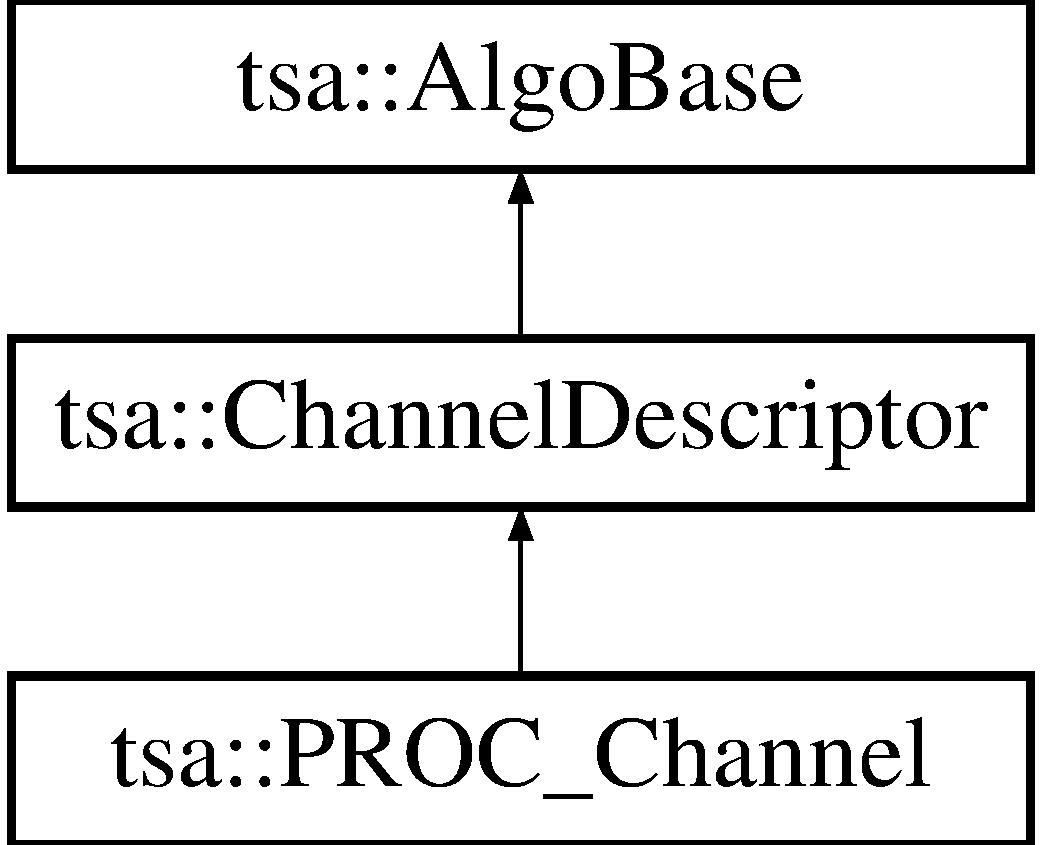
\includegraphics[height=3.000000cm]{classtsa_1_1_p_r_o_c___channel}
\end{center}
\end{figure}
\subsection*{Public Member Functions}
\begin{DoxyCompactItemize}
\item 
\hyperlink{classtsa_1_1_p_r_o_c___channel_ab92dfa656aaf23e89436ba364d573980}{P\+R\+O\+C\+\_\+\+Channel} (\hyperlink{classtsa_1_1_frame_i_stream}{Frame\+I\+Stream} $\ast$F\+IS, Fr\+Proc\+Data $\ast$proc, unsigned int id)
\item 
virtual \hyperlink{classtsa_1_1_p_r_o_c___channel_acba6a69209ee63e13427046085d2be8d}{$\sim$\+P\+R\+O\+C\+\_\+\+Channel} ()
\item 
virtual void \hyperlink{classtsa_1_1_p_r_o_c___channel_ab4f986f7829c52ca6c0d8c244be7c617}{Add\+Data} ()
\item 
virtual double \hyperlink{classtsa_1_1_p_r_o_c___channel_ac29ae55cbededca3814b30e1186a4650}{Get\+Length} ()
\item 
virtual void \hyperlink{classtsa_1_1_p_r_o_c___channel_a84f00b22077b0aa41dba95ac0aaf0478}{Fill\+View} (\hyperlink{namespacetsa_ac599574bcc094eda25613724b8f3ca9e}{Seq\+View\+Double} \&v, double tstart, double tend)
\end{DoxyCompactItemize}
\subsection*{Static Public Member Functions}
\begin{DoxyCompactItemize}
\item 
static \hyperlink{classtsa_1_1_p_r_o_c___channel}{P\+R\+O\+C\+\_\+\+Channel} $\ast$ \hyperlink{classtsa_1_1_p_r_o_c___channel_ae1d07e5c6af50796d0e97e4258807521}{Create} (\hyperlink{classtsa_1_1_frame_i_stream}{Frame\+I\+Stream} $\ast$F\+IS, char $\ast$name, unsigned int id)
\end{DoxyCompactItemize}
\subsection*{Private Attributes}
\begin{DoxyCompactItemize}
\item 
char $\ast$ \hyperlink{classtsa_1_1_p_r_o_c___channel_a81ce6bd37c7c57c76da43519841e0c85}{m\+Name}
\end{DoxyCompactItemize}
\subsection*{Additional Inherited Members}


\subsection{Detailed Description}
A descriptor for a proc channel 

Definition at line 285 of file Frame\+I\+Stream.\+hpp.



\subsection{Constructor \& Destructor Documentation}
\mbox{\Hypertarget{classtsa_1_1_p_r_o_c___channel_ab92dfa656aaf23e89436ba364d573980}\label{classtsa_1_1_p_r_o_c___channel_ab92dfa656aaf23e89436ba364d573980}} 
\index{tsa\+::\+P\+R\+O\+C\+\_\+\+Channel@{tsa\+::\+P\+R\+O\+C\+\_\+\+Channel}!P\+R\+O\+C\+\_\+\+Channel@{P\+R\+O\+C\+\_\+\+Channel}}
\index{P\+R\+O\+C\+\_\+\+Channel@{P\+R\+O\+C\+\_\+\+Channel}!tsa\+::\+P\+R\+O\+C\+\_\+\+Channel@{tsa\+::\+P\+R\+O\+C\+\_\+\+Channel}}
\subsubsection{\texorpdfstring{P\+R\+O\+C\+\_\+\+Channel()}{PROC\_Channel()}}
{\footnotesize\ttfamily tsa\+::\+P\+R\+O\+C\+\_\+\+Channel\+::\+P\+R\+O\+C\+\_\+\+Channel (\begin{DoxyParamCaption}\item[{\hyperlink{classtsa_1_1_frame_i_stream}{Frame\+I\+Stream} $\ast$}]{F\+IS,  }\item[{Fr\+Proc\+Data $\ast$}]{proc,  }\item[{unsigned int}]{id }\end{DoxyParamCaption})}

Constructor


\begin{DoxyParams}{Parameters}
{\em F\+IS} & pointer to the \hyperlink{classtsa_1_1_frame_i_stream}{Frame\+I\+Stream} class \\
\hline
{\em proc} & pointer to the first Fr\+Proc\+Data structure \\
\hline
{\em id} & id of the channel \\
\hline
\end{DoxyParams}


Definition at line 269 of file Frame\+I\+Stream.\+cpp.

\mbox{\Hypertarget{classtsa_1_1_p_r_o_c___channel_acba6a69209ee63e13427046085d2be8d}\label{classtsa_1_1_p_r_o_c___channel_acba6a69209ee63e13427046085d2be8d}} 
\index{tsa\+::\+P\+R\+O\+C\+\_\+\+Channel@{tsa\+::\+P\+R\+O\+C\+\_\+\+Channel}!````~P\+R\+O\+C\+\_\+\+Channel@{$\sim$\+P\+R\+O\+C\+\_\+\+Channel}}
\index{````~P\+R\+O\+C\+\_\+\+Channel@{$\sim$\+P\+R\+O\+C\+\_\+\+Channel}!tsa\+::\+P\+R\+O\+C\+\_\+\+Channel@{tsa\+::\+P\+R\+O\+C\+\_\+\+Channel}}
\subsubsection{\texorpdfstring{$\sim$\+P\+R\+O\+C\+\_\+\+Channel()}{~PROC\_Channel()}}
{\footnotesize\ttfamily tsa\+::\+P\+R\+O\+C\+\_\+\+Channel\+::$\sim$\+P\+R\+O\+C\+\_\+\+Channel (\begin{DoxyParamCaption}{ }\end{DoxyParamCaption})\hspace{0.3cm}{\ttfamily [virtual]}}

Destructor 

Definition at line 281 of file Frame\+I\+Stream.\+cpp.



\subsection{Member Function Documentation}
\mbox{\Hypertarget{classtsa_1_1_p_r_o_c___channel_ab4f986f7829c52ca6c0d8c244be7c617}\label{classtsa_1_1_p_r_o_c___channel_ab4f986f7829c52ca6c0d8c244be7c617}} 
\index{tsa\+::\+P\+R\+O\+C\+\_\+\+Channel@{tsa\+::\+P\+R\+O\+C\+\_\+\+Channel}!Add\+Data@{Add\+Data}}
\index{Add\+Data@{Add\+Data}!tsa\+::\+P\+R\+O\+C\+\_\+\+Channel@{tsa\+::\+P\+R\+O\+C\+\_\+\+Channel}}
\subsubsection{\texorpdfstring{Add\+Data()}{AddData()}}
{\footnotesize\ttfamily void tsa\+::\+P\+R\+O\+C\+\_\+\+Channel\+::\+Add\+Data (\begin{DoxyParamCaption}{ }\end{DoxyParamCaption})\hspace{0.3cm}{\ttfamily [virtual]}}

This function must be called when there are not enough data to fill the output view. It reads a chunk of data from the next Fr\+Proc\+Data structure. 

Reimplemented from \hyperlink{classtsa_1_1_channel_descriptor_aa1e001a5e712415cd4e9d66846914a56}{tsa\+::\+Channel\+Descriptor}.



Definition at line 285 of file Frame\+I\+Stream.\+cpp.

\mbox{\Hypertarget{classtsa_1_1_p_r_o_c___channel_ae1d07e5c6af50796d0e97e4258807521}\label{classtsa_1_1_p_r_o_c___channel_ae1d07e5c6af50796d0e97e4258807521}} 
\index{tsa\+::\+P\+R\+O\+C\+\_\+\+Channel@{tsa\+::\+P\+R\+O\+C\+\_\+\+Channel}!Create@{Create}}
\index{Create@{Create}!tsa\+::\+P\+R\+O\+C\+\_\+\+Channel@{tsa\+::\+P\+R\+O\+C\+\_\+\+Channel}}
\subsubsection{\texorpdfstring{Create()}{Create()}}
{\footnotesize\ttfamily \hyperlink{classtsa_1_1_p_r_o_c___channel}{P\+R\+O\+C\+\_\+\+Channel} $\ast$ tsa\+::\+P\+R\+O\+C\+\_\+\+Channel\+::\+Create (\begin{DoxyParamCaption}\item[{\hyperlink{classtsa_1_1_frame_i_stream}{Frame\+I\+Stream} $\ast$}]{F\+IS,  }\item[{char $\ast$}]{name,  }\item[{unsigned int}]{id }\end{DoxyParamCaption})\hspace{0.3cm}{\ttfamily [static]}}

Create, if possible, an instance of the class


\begin{DoxyParams}{Parameters}
{\em F\+IS} & pointer to the \hyperlink{classtsa_1_1_frame_i_stream}{Frame\+I\+Stream} class instance \\
\hline
{\em name} & name of the channel \\
\hline
{\em id} & index of the channel\\
\hline
\end{DoxyParams}
\begin{DoxyReturn}{Returns}
pointer to the created class instance or null 
\end{DoxyReturn}


Definition at line 258 of file Frame\+I\+Stream.\+cpp.

\mbox{\Hypertarget{classtsa_1_1_p_r_o_c___channel_a84f00b22077b0aa41dba95ac0aaf0478}\label{classtsa_1_1_p_r_o_c___channel_a84f00b22077b0aa41dba95ac0aaf0478}} 
\index{tsa\+::\+P\+R\+O\+C\+\_\+\+Channel@{tsa\+::\+P\+R\+O\+C\+\_\+\+Channel}!Fill\+View@{Fill\+View}}
\index{Fill\+View@{Fill\+View}!tsa\+::\+P\+R\+O\+C\+\_\+\+Channel@{tsa\+::\+P\+R\+O\+C\+\_\+\+Channel}}
\subsubsection{\texorpdfstring{Fill\+View()}{FillView()}}
{\footnotesize\ttfamily void tsa\+::\+P\+R\+O\+C\+\_\+\+Channel\+::\+Fill\+View (\begin{DoxyParamCaption}\item[{\hyperlink{namespacetsa_ac599574bcc094eda25613724b8f3ca9e}{Seq\+View\+Double} \&}]{v,  }\item[{double}]{tstart,  }\item[{double}]{tend }\end{DoxyParamCaption})\hspace{0.3cm}{\ttfamily [virtual]}}



Reimplemented from \hyperlink{classtsa_1_1_channel_descriptor_a6553da04ba33471fc5465b6bd2b5275c}{tsa\+::\+Channel\+Descriptor}.



Definition at line 298 of file Frame\+I\+Stream.\+cpp.

\mbox{\Hypertarget{classtsa_1_1_p_r_o_c___channel_ac29ae55cbededca3814b30e1186a4650}\label{classtsa_1_1_p_r_o_c___channel_ac29ae55cbededca3814b30e1186a4650}} 
\index{tsa\+::\+P\+R\+O\+C\+\_\+\+Channel@{tsa\+::\+P\+R\+O\+C\+\_\+\+Channel}!Get\+Length@{Get\+Length}}
\index{Get\+Length@{Get\+Length}!tsa\+::\+P\+R\+O\+C\+\_\+\+Channel@{tsa\+::\+P\+R\+O\+C\+\_\+\+Channel}}
\subsubsection{\texorpdfstring{Get\+Length()}{GetLength()}}
{\footnotesize\ttfamily double tsa\+::\+P\+R\+O\+C\+\_\+\+Channel\+::\+Get\+Length (\begin{DoxyParamCaption}{ }\end{DoxyParamCaption})\hspace{0.3cm}{\ttfamily [virtual]}}

Get the maximul time length of data that can be currently filled without calling Add\+Data.

\begin{DoxyReturn}{Returns}
the time length of the data available in seconds 
\end{DoxyReturn}


Reimplemented from \hyperlink{classtsa_1_1_channel_descriptor_a456d14e6136c389fbd307fabab7d7b73}{tsa\+::\+Channel\+Descriptor}.



Definition at line 294 of file Frame\+I\+Stream.\+cpp.



\subsection{Member Data Documentation}
\mbox{\Hypertarget{classtsa_1_1_p_r_o_c___channel_a81ce6bd37c7c57c76da43519841e0c85}\label{classtsa_1_1_p_r_o_c___channel_a81ce6bd37c7c57c76da43519841e0c85}} 
\index{tsa\+::\+P\+R\+O\+C\+\_\+\+Channel@{tsa\+::\+P\+R\+O\+C\+\_\+\+Channel}!m\+Name@{m\+Name}}
\index{m\+Name@{m\+Name}!tsa\+::\+P\+R\+O\+C\+\_\+\+Channel@{tsa\+::\+P\+R\+O\+C\+\_\+\+Channel}}
\subsubsection{\texorpdfstring{m\+Name}{mName}}
{\footnotesize\ttfamily char$\ast$ tsa\+::\+P\+R\+O\+C\+\_\+\+Channel\+::m\+Name\hspace{0.3cm}{\ttfamily [private]}}

The channel\textquotesingle{}s name 

Definition at line 335 of file Frame\+I\+Stream.\+hpp.



The documentation for this class was generated from the following files\+:\begin{DoxyCompactItemize}
\item 
/home/filip/\+Ph\+D/\+W\+D\+F\+Pipe\+\_\+test/p4\+T\+S\+A/include/\hyperlink{_frame_i_stream_8hpp}{Frame\+I\+Stream.\+hpp}\item 
/home/filip/\+Ph\+D/\+W\+D\+F\+Pipe\+\_\+test/p4\+T\+S\+A/src/\hyperlink{_frame_i_stream_8cpp}{Frame\+I\+Stream.\+cpp}\end{DoxyCompactItemize}

\hypertarget{classtsa_1_1quality__change}{}\section{tsa\+:\+:quality\+\_\+change Class Reference}
\label{classtsa_1_1quality__change}\index{tsa\+::quality\+\_\+change@{tsa\+::quality\+\_\+change}}


{\ttfamily \#include $<$Algo\+Exceptions.\+hpp$>$}

Inheritance diagram for tsa\+:\+:quality\+\_\+change\+:\begin{figure}[H]
\begin{center}
\leavevmode
\includegraphics[height=2.000000cm]{classtsa_1_1quality__change}
\end{center}
\end{figure}
\subsection*{Public Member Functions}
\begin{DoxyCompactItemize}
\item 
\hyperlink{classtsa_1_1quality__change_af530cc58e7eeb50f31ddb700bfea79f4}{quality\+\_\+change} (const std\+::string \&msg, double change\+\_\+time, unsigned int old\+\_\+flag, unsigned int new\+\_\+flag)
\item 
double \hyperlink{classtsa_1_1quality__change_a71190c89b87f044b190e67be16f4c1a4}{Event\+Time} ()
\item 
unsigned int \hyperlink{classtsa_1_1quality__change_af1f74fabce5ad05c2088a7e99a68cb6a}{Old\+Flag} ()
\item 
unsigned int \hyperlink{classtsa_1_1quality__change_a6de5d5aea1cf03c5d4d2d69014d78d2d}{New\+Flag} ()
\end{DoxyCompactItemize}
\subsection*{Private Attributes}
\begin{DoxyCompactItemize}
\item 
double \hyperlink{classtsa_1_1quality__change_a5bbdd6247455082169c25acf8c092186}{m\+Event\+Time}
\item 
unsigned int \hyperlink{classtsa_1_1quality__change_aca073076da85ec9eab1fa6d9b7e99a2b}{m\+Old\+Flag}
\item 
unsigned int \hyperlink{classtsa_1_1quality__change_a90e75c508ba37e01d11727853e401919}{m\+New\+Flag}
\end{DoxyCompactItemize}


\subsection{Detailed Description}
This exception should be used when data quality change 

Definition at line 207 of file Algo\+Exceptions.\+hpp.



\subsection{Constructor \& Destructor Documentation}
\mbox{\Hypertarget{classtsa_1_1quality__change_af530cc58e7eeb50f31ddb700bfea79f4}\label{classtsa_1_1quality__change_af530cc58e7eeb50f31ddb700bfea79f4}} 
\index{tsa\+::quality\+\_\+change@{tsa\+::quality\+\_\+change}!quality\+\_\+change@{quality\+\_\+change}}
\index{quality\+\_\+change@{quality\+\_\+change}!tsa\+::quality\+\_\+change@{tsa\+::quality\+\_\+change}}
\subsubsection{\texorpdfstring{quality\+\_\+change()}{quality\_change()}}
{\footnotesize\ttfamily tsa\+::quality\+\_\+change\+::quality\+\_\+change (\begin{DoxyParamCaption}\item[{const std\+::string \&}]{msg,  }\item[{double}]{change\+\_\+time,  }\item[{unsigned int}]{old\+\_\+flag,  }\item[{unsigned int}]{new\+\_\+flag }\end{DoxyParamCaption})\hspace{0.3cm}{\ttfamily [inline]}}

Constructor


\begin{DoxyParams}{Parameters}
{\em msg} & error message \\
\hline
\end{DoxyParams}


Definition at line 215 of file Algo\+Exceptions.\+hpp.



\subsection{Member Function Documentation}
\mbox{\Hypertarget{classtsa_1_1quality__change_a71190c89b87f044b190e67be16f4c1a4}\label{classtsa_1_1quality__change_a71190c89b87f044b190e67be16f4c1a4}} 
\index{tsa\+::quality\+\_\+change@{tsa\+::quality\+\_\+change}!Event\+Time@{Event\+Time}}
\index{Event\+Time@{Event\+Time}!tsa\+::quality\+\_\+change@{tsa\+::quality\+\_\+change}}
\subsubsection{\texorpdfstring{Event\+Time()}{EventTime()}}
{\footnotesize\ttfamily double tsa\+::quality\+\_\+change\+::\+Event\+Time (\begin{DoxyParamCaption}{ }\end{DoxyParamCaption})\hspace{0.3cm}{\ttfamily [inline]}}



Definition at line 224 of file Algo\+Exceptions.\+hpp.

\mbox{\Hypertarget{classtsa_1_1quality__change_a6de5d5aea1cf03c5d4d2d69014d78d2d}\label{classtsa_1_1quality__change_a6de5d5aea1cf03c5d4d2d69014d78d2d}} 
\index{tsa\+::quality\+\_\+change@{tsa\+::quality\+\_\+change}!New\+Flag@{New\+Flag}}
\index{New\+Flag@{New\+Flag}!tsa\+::quality\+\_\+change@{tsa\+::quality\+\_\+change}}
\subsubsection{\texorpdfstring{New\+Flag()}{NewFlag()}}
{\footnotesize\ttfamily unsigned int tsa\+::quality\+\_\+change\+::\+New\+Flag (\begin{DoxyParamCaption}{ }\end{DoxyParamCaption})\hspace{0.3cm}{\ttfamily [inline]}}



Definition at line 232 of file Algo\+Exceptions.\+hpp.

\mbox{\Hypertarget{classtsa_1_1quality__change_af1f74fabce5ad05c2088a7e99a68cb6a}\label{classtsa_1_1quality__change_af1f74fabce5ad05c2088a7e99a68cb6a}} 
\index{tsa\+::quality\+\_\+change@{tsa\+::quality\+\_\+change}!Old\+Flag@{Old\+Flag}}
\index{Old\+Flag@{Old\+Flag}!tsa\+::quality\+\_\+change@{tsa\+::quality\+\_\+change}}
\subsubsection{\texorpdfstring{Old\+Flag()}{OldFlag()}}
{\footnotesize\ttfamily unsigned int tsa\+::quality\+\_\+change\+::\+Old\+Flag (\begin{DoxyParamCaption}{ }\end{DoxyParamCaption})\hspace{0.3cm}{\ttfamily [inline]}}



Definition at line 228 of file Algo\+Exceptions.\+hpp.



\subsection{Member Data Documentation}
\mbox{\Hypertarget{classtsa_1_1quality__change_a5bbdd6247455082169c25acf8c092186}\label{classtsa_1_1quality__change_a5bbdd6247455082169c25acf8c092186}} 
\index{tsa\+::quality\+\_\+change@{tsa\+::quality\+\_\+change}!m\+Event\+Time@{m\+Event\+Time}}
\index{m\+Event\+Time@{m\+Event\+Time}!tsa\+::quality\+\_\+change@{tsa\+::quality\+\_\+change}}
\subsubsection{\texorpdfstring{m\+Event\+Time}{mEventTime}}
{\footnotesize\ttfamily double tsa\+::quality\+\_\+change\+::m\+Event\+Time\hspace{0.3cm}{\ttfamily [private]}}



Definition at line 236 of file Algo\+Exceptions.\+hpp.

\mbox{\Hypertarget{classtsa_1_1quality__change_a90e75c508ba37e01d11727853e401919}\label{classtsa_1_1quality__change_a90e75c508ba37e01d11727853e401919}} 
\index{tsa\+::quality\+\_\+change@{tsa\+::quality\+\_\+change}!m\+New\+Flag@{m\+New\+Flag}}
\index{m\+New\+Flag@{m\+New\+Flag}!tsa\+::quality\+\_\+change@{tsa\+::quality\+\_\+change}}
\subsubsection{\texorpdfstring{m\+New\+Flag}{mNewFlag}}
{\footnotesize\ttfamily unsigned int tsa\+::quality\+\_\+change\+::m\+New\+Flag\hspace{0.3cm}{\ttfamily [private]}}



Definition at line 238 of file Algo\+Exceptions.\+hpp.

\mbox{\Hypertarget{classtsa_1_1quality__change_aca073076da85ec9eab1fa6d9b7e99a2b}\label{classtsa_1_1quality__change_aca073076da85ec9eab1fa6d9b7e99a2b}} 
\index{tsa\+::quality\+\_\+change@{tsa\+::quality\+\_\+change}!m\+Old\+Flag@{m\+Old\+Flag}}
\index{m\+Old\+Flag@{m\+Old\+Flag}!tsa\+::quality\+\_\+change@{tsa\+::quality\+\_\+change}}
\subsubsection{\texorpdfstring{m\+Old\+Flag}{mOldFlag}}
{\footnotesize\ttfamily unsigned int tsa\+::quality\+\_\+change\+::m\+Old\+Flag\hspace{0.3cm}{\ttfamily [private]}}



Definition at line 237 of file Algo\+Exceptions.\+hpp.



The documentation for this class was generated from the following file\+:\begin{DoxyCompactItemize}
\item 
/home/filip/\+Ph\+D/\+W\+D\+F\+Pipe\+\_\+test/p4\+T\+S\+A/include/\hyperlink{_algo_exceptions_8hpp}{Algo\+Exceptions.\+hpp}\end{DoxyCompactItemize}

\hypertarget{classtsa_1_1_real_f_f_t}{}\section{tsa\+:\+:Real\+F\+FT Class Reference}
\label{classtsa_1_1_real_f_f_t}\index{tsa\+::\+Real\+F\+FT@{tsa\+::\+Real\+F\+FT}}


Multichannel real to complex F\+FT.  




{\ttfamily \#include $<$Real\+F\+F\+T.\+hpp$>$}

Inheritance diagram for tsa\+:\+:Real\+F\+FT\+:\begin{figure}[H]
\begin{center}
\leavevmode
\includegraphics[height=3.000000cm]{classtsa_1_1_real_f_f_t}
\end{center}
\end{figure}
\subsection*{Public Member Functions}
\begin{DoxyCompactItemize}
\item 
\hyperlink{classtsa_1_1_real_f_f_t_a5da04120c5120c230282a6833b8871ae}{Real\+F\+FT} (int size=0, enum \hyperlink{namespacetsa_a217e07ef78939f88b22c8428ac96b1ae}{F\+F\+T\+Planning\+Mode} mode=\hyperlink{namespacetsa_a217e07ef78939f88b22c8428ac96b1aea2762be66fb6f3e4772c7f4cc162b9750}{E\+S\+T\+I\+M\+A\+TE}, bool Preserve\+Input=true)
\item 
\hyperlink{classtsa_1_1_real_f_f_t_a2c65c00ea09121cceb8804b9d5e1c395}{Real\+F\+FT} (const \hyperlink{classtsa_1_1_real_f_f_t}{Real\+F\+FT} \&from)
\item 
virtual \hyperlink{classtsa_1_1_real_f_f_t_a51eccd426b1802e0c245c8dd4006dc3e}{$\sim$\+Real\+F\+FT} ()
\end{DoxyCompactItemize}
\begin{Indent}\textbf{ Operations}\par
\begin{DoxyCompactItemize}
\item 
void \hyperlink{classtsa_1_1_real_f_f_t_a3bf380302985631f972017262e83be11}{operator()} (\hyperlink{namespacetsa_ac599574bcc094eda25613724b8f3ca9e}{Seq\+View\+Double} \&in, \hyperlink{namespacetsa_ab32775c889b53c40fa83939f22372b75}{Seq\+View\+Complex} \&out)
\item 
void \hyperlink{classtsa_1_1_real_f_f_t_a571915c01137937b542c88c3094b9e50}{execute} (\hyperlink{namespacetsa_ad260cd21c1891c4ed391fe788569aba4}{Dmatrix} \&in, \hyperlink{namespacetsa_a86348fef1603a135fe5fba9e5f5486ee}{Cmatrix} \&out)  throw (bad\+\_\+matrix\+\_\+size)
\item 
void \hyperlink{classtsa_1_1_real_f_f_t_a8315388a35738d3005bc596852500e56}{execute} (\hyperlink{namespacetsa_ad260cd21c1891c4ed391fe788569aba4}{Dmatrix} \&indata, \hyperlink{namespacetsa_a86348fef1603a135fe5fba9e5f5486ee}{Cmatrix} \&outdata, unsigned int size, unsigned int offset)  throw (bad\+\_\+matrix\+\_\+size)
\item 
void \hyperlink{classtsa_1_1_real_f_f_t_a14b6f0098aed4984d7b969f107df5f2b}{execute} (\hyperlink{namespacetsa_a8900fb03d849baf447a1a0efe2561fb2}{Dvector} \&in, \hyperlink{namespacetsa_a054d1045ead95a65819e9e5722baf600}{Cvector} \&out)  throw (bad\+\_\+vector\+\_\+size)
\item 
void \hyperlink{classtsa_1_1_real_f_f_t_a6684b1abf6f9de2d7c546c3556ef0a0e}{Make\+Plan} ()  throw (std\+::runtime\+\_\+error)
\end{DoxyCompactItemize}
\end{Indent}
\subsection*{Additional Inherited Members}


\subsection{Detailed Description}
Multichannel real to complex F\+FT. 

This is the implementation of the F\+FT of a real multichannel buffer 

Definition at line 74 of file Real\+F\+F\+T.\+hpp.



\subsection{Constructor \& Destructor Documentation}
\mbox{\Hypertarget{classtsa_1_1_real_f_f_t_a5da04120c5120c230282a6833b8871ae}\label{classtsa_1_1_real_f_f_t_a5da04120c5120c230282a6833b8871ae}} 
\index{tsa\+::\+Real\+F\+FT@{tsa\+::\+Real\+F\+FT}!Real\+F\+FT@{Real\+F\+FT}}
\index{Real\+F\+FT@{Real\+F\+FT}!tsa\+::\+Real\+F\+FT@{tsa\+::\+Real\+F\+FT}}
\subsubsection{\texorpdfstring{Real\+F\+F\+T()}{RealFFT()}\hspace{0.1cm}{\footnotesize\ttfamily [1/2]}}
{\footnotesize\ttfamily tsa\+::\+Real\+F\+F\+T\+::\+Real\+F\+FT (\begin{DoxyParamCaption}\item[{int}]{size = {\ttfamily 0},  }\item[{enum \hyperlink{namespacetsa_a217e07ef78939f88b22c8428ac96b1ae}{F\+F\+T\+Planning\+Mode}}]{mode = {\ttfamily \hyperlink{namespacetsa_a217e07ef78939f88b22c8428ac96b1aea2762be66fb6f3e4772c7f4cc162b9750}{E\+S\+T\+I\+M\+A\+TE}},  }\item[{bool}]{Preserve\+Input = {\ttfamily true} }\end{DoxyParamCaption})}

Constructor


\begin{DoxyParams}{Parameters}
{\em size} & the size of the transform \\
\hline
{\em mode} & specify the way in which plans are calculated \\
\hline
{\em Preserve\+Input} & true if the input buffer must be preserved during the transform, false otherwise \\
\hline
\end{DoxyParams}


Definition at line 5 of file Real\+F\+F\+T.\+cpp.

\mbox{\Hypertarget{classtsa_1_1_real_f_f_t_a2c65c00ea09121cceb8804b9d5e1c395}\label{classtsa_1_1_real_f_f_t_a2c65c00ea09121cceb8804b9d5e1c395}} 
\index{tsa\+::\+Real\+F\+FT@{tsa\+::\+Real\+F\+FT}!Real\+F\+FT@{Real\+F\+FT}}
\index{Real\+F\+FT@{Real\+F\+FT}!tsa\+::\+Real\+F\+FT@{tsa\+::\+Real\+F\+FT}}
\subsubsection{\texorpdfstring{Real\+F\+F\+T()}{RealFFT()}\hspace{0.1cm}{\footnotesize\ttfamily [2/2]}}
{\footnotesize\ttfamily tsa\+::\+Real\+F\+F\+T\+::\+Real\+F\+FT (\begin{DoxyParamCaption}\item[{const \hyperlink{classtsa_1_1_real_f_f_t}{Real\+F\+FT} \&}]{from }\end{DoxyParamCaption})}

Copy constructor


\begin{DoxyParams}{Parameters}
{\em from} & The instance that must be copied \\
\hline
\end{DoxyParams}


Definition at line 11 of file Real\+F\+F\+T.\+cpp.

\mbox{\Hypertarget{classtsa_1_1_real_f_f_t_a51eccd426b1802e0c245c8dd4006dc3e}\label{classtsa_1_1_real_f_f_t_a51eccd426b1802e0c245c8dd4006dc3e}} 
\index{tsa\+::\+Real\+F\+FT@{tsa\+::\+Real\+F\+FT}!````~Real\+F\+FT@{$\sim$\+Real\+F\+FT}}
\index{````~Real\+F\+FT@{$\sim$\+Real\+F\+FT}!tsa\+::\+Real\+F\+FT@{tsa\+::\+Real\+F\+FT}}
\subsubsection{\texorpdfstring{$\sim$\+Real\+F\+F\+T()}{~RealFFT()}}
{\footnotesize\ttfamily tsa\+::\+Real\+F\+F\+T\+::$\sim$\+Real\+F\+FT (\begin{DoxyParamCaption}{ }\end{DoxyParamCaption})\hspace{0.3cm}{\ttfamily [virtual]}}

Destructor 

Definition at line 17 of file Real\+F\+F\+T.\+cpp.



\subsection{Member Function Documentation}
\mbox{\Hypertarget{classtsa_1_1_real_f_f_t_a571915c01137937b542c88c3094b9e50}\label{classtsa_1_1_real_f_f_t_a571915c01137937b542c88c3094b9e50}} 
\index{tsa\+::\+Real\+F\+FT@{tsa\+::\+Real\+F\+FT}!execute@{execute}}
\index{execute@{execute}!tsa\+::\+Real\+F\+FT@{tsa\+::\+Real\+F\+FT}}
\subsubsection{\texorpdfstring{execute()}{execute()}\hspace{0.1cm}{\footnotesize\ttfamily [1/3]}}
{\footnotesize\ttfamily void tsa\+::\+Real\+F\+F\+T\+::execute (\begin{DoxyParamCaption}\item[{\hyperlink{namespacetsa_ad260cd21c1891c4ed391fe788569aba4}{Dmatrix} \&}]{in,  }\item[{\hyperlink{namespacetsa_a86348fef1603a135fe5fba9e5f5486ee}{Cmatrix} \&}]{out }\end{DoxyParamCaption}) throw  \hyperlink{classtsa_1_1bad__matrix__size}{bad\+\_\+matrix\+\_\+size}) }

Execution of the fft of a multichannel buffer of double. Input data are organized in a matrix. Each row is a different channel, and the number of data to transform is equal to the number of columns. Both the number of rows and the number of columns can change between each call to this method. If the number of rows changes nothing special will happen, if the number of cols changes the plan is reevaluated with the current flags.

\begin{DoxyPrecond}{Precondition}
The number of rows of input and output matrix must be the same. 

The columns of the output matrix must be int(n/2)+1, where n is the number of columns of the input matrix.
\end{DoxyPrecond}
\begin{DoxyPostcond}{Postcondition}
the input buffer is unchanged, unless Set\+Preserve\+Input(false) was called 

the output buffer contain the fft of the input data
\end{DoxyPostcond}

\begin{DoxyExceptions}{Exceptions}
{\em \hyperlink{classtsa_1_1bad__matrix__size}{bad\+\_\+matrix\+\_\+size}} & the size of the output matrix is wrong \\
\hline
\end{DoxyExceptions}

\begin{DoxyParams}{Parameters}
{\em in} & reference to the input multichannel buffer \\
\hline
{\em out} & reference to the output multichannel buffer \\
\hline
\end{DoxyParams}


Definition at line 41 of file Real\+F\+F\+T.\+cpp.

\mbox{\Hypertarget{classtsa_1_1_real_f_f_t_a8315388a35738d3005bc596852500e56}\label{classtsa_1_1_real_f_f_t_a8315388a35738d3005bc596852500e56}} 
\index{tsa\+::\+Real\+F\+FT@{tsa\+::\+Real\+F\+FT}!execute@{execute}}
\index{execute@{execute}!tsa\+::\+Real\+F\+FT@{tsa\+::\+Real\+F\+FT}}
\subsubsection{\texorpdfstring{execute()}{execute()}\hspace{0.1cm}{\footnotesize\ttfamily [2/3]}}
{\footnotesize\ttfamily void tsa\+::\+Real\+F\+F\+T\+::execute (\begin{DoxyParamCaption}\item[{\hyperlink{namespacetsa_ad260cd21c1891c4ed391fe788569aba4}{Dmatrix} \&}]{indata,  }\item[{\hyperlink{namespacetsa_a86348fef1603a135fe5fba9e5f5486ee}{Cmatrix} \&}]{outdata,  }\item[{unsigned int}]{size,  }\item[{unsigned int}]{offset }\end{DoxyParamCaption}) throw  \hyperlink{classtsa_1_1bad__matrix__size}{bad\+\_\+matrix\+\_\+size}) }



Definition at line 73 of file Real\+F\+F\+T.\+cpp.

\mbox{\Hypertarget{classtsa_1_1_real_f_f_t_a14b6f0098aed4984d7b969f107df5f2b}\label{classtsa_1_1_real_f_f_t_a14b6f0098aed4984d7b969f107df5f2b}} 
\index{tsa\+::\+Real\+F\+FT@{tsa\+::\+Real\+F\+FT}!execute@{execute}}
\index{execute@{execute}!tsa\+::\+Real\+F\+FT@{tsa\+::\+Real\+F\+FT}}
\subsubsection{\texorpdfstring{execute()}{execute()}\hspace{0.1cm}{\footnotesize\ttfamily [3/3]}}
{\footnotesize\ttfamily void tsa\+::\+Real\+F\+F\+T\+::execute (\begin{DoxyParamCaption}\item[{\hyperlink{namespacetsa_a8900fb03d849baf447a1a0efe2561fb2}{Dvector} \&}]{in,  }\item[{\hyperlink{namespacetsa_a054d1045ead95a65819e9e5722baf600}{Cvector} \&}]{out }\end{DoxyParamCaption}) throw  \hyperlink{classtsa_1_1bad__vector__size}{bad\+\_\+vector\+\_\+size}) }

Execution of the fft of a single channel buffer of double. If the number of the buffer changes the plan is reevaluated with the current flags.

\begin{DoxyPrecond}{Precondition}
The sized of the output vector must be int(n/2)+1, where n is the size of the input vector.
\end{DoxyPrecond}
\begin{DoxyPostcond}{Postcondition}
the input buffer is unchanged, unless Set\+Preserve\+Input(false) was called 

the output buffer contain the fft of the input data
\end{DoxyPostcond}

\begin{DoxyExceptions}{Exceptions}
{\em \hyperlink{classtsa_1_1bad__matrix__size}{bad\+\_\+matrix\+\_\+size}} & the size of the output matrix is wrong \\
\hline
\end{DoxyExceptions}

\begin{DoxyParams}{Parameters}
{\em in} & reference to the input buffer \\
\hline
{\em out} & reference to the output buffer \\
\hline
\end{DoxyParams}


Definition at line 103 of file Real\+F\+F\+T.\+cpp.

\mbox{\Hypertarget{classtsa_1_1_real_f_f_t_a6684b1abf6f9de2d7c546c3556ef0a0e}\label{classtsa_1_1_real_f_f_t_a6684b1abf6f9de2d7c546c3556ef0a0e}} 
\index{tsa\+::\+Real\+F\+FT@{tsa\+::\+Real\+F\+FT}!Make\+Plan@{Make\+Plan}}
\index{Make\+Plan@{Make\+Plan}!tsa\+::\+Real\+F\+FT@{tsa\+::\+Real\+F\+FT}}
\subsubsection{\texorpdfstring{Make\+Plan()}{MakePlan()}}
{\footnotesize\ttfamily void tsa\+::\+Real\+F\+F\+T\+::\+Make\+Plan (\begin{DoxyParamCaption}{ }\end{DoxyParamCaption}) throw  std\+::runtime\+\_\+error) \hspace{0.3cm}{\ttfamily [virtual]}}

Make a new plan, with the current parameters.


\begin{DoxyExceptions}{Exceptions}
{\em std\+::runtime\+\_\+error} & The new plan cannot be created \\
\hline
\end{DoxyExceptions}


Implements \hyperlink{classtsa_1_1_base_f_f_t_a9af0c36413173821cac8dbdce9cfe3b4}{tsa\+::\+Base\+F\+FT}.



Definition at line 127 of file Real\+F\+F\+T.\+cpp.

\mbox{\Hypertarget{classtsa_1_1_real_f_f_t_a3bf380302985631f972017262e83be11}\label{classtsa_1_1_real_f_f_t_a3bf380302985631f972017262e83be11}} 
\index{tsa\+::\+Real\+F\+FT@{tsa\+::\+Real\+F\+FT}!operator()@{operator()}}
\index{operator()@{operator()}!tsa\+::\+Real\+F\+FT@{tsa\+::\+Real\+F\+FT}}
\subsubsection{\texorpdfstring{operator()()}{operator()()}}
{\footnotesize\ttfamily void tsa\+::\+Real\+F\+F\+T\+::operator() (\begin{DoxyParamCaption}\item[{\hyperlink{namespacetsa_ac599574bcc094eda25613724b8f3ca9e}{Seq\+View\+Double} \&}]{in,  }\item[{\hyperlink{namespacetsa_ab32775c889b53c40fa83939f22372b75}{Seq\+View\+Complex} \&}]{out }\end{DoxyParamCaption})}

Apply the transformation on the data


\begin{DoxyParams}{Parameters}
{\em in} & a reference to the buffer containing the input data \\
\hline
{\em out} & a reference to the buffer containing the input data\\
\hline
\end{DoxyParams}
\begin{DoxyReturn}{Returns}
a reference to this instance of the class 
\end{DoxyReturn}


Definition at line 21 of file Real\+F\+F\+T.\+cpp.



The documentation for this class was generated from the following files\+:\begin{DoxyCompactItemize}
\item 
/home/filip/\+Ph\+D/\+W\+D\+F\+Pipe\+\_\+test/p4\+T\+S\+A/include/\hyperlink{_real_f_f_t_8hpp}{Real\+F\+F\+T.\+hpp}\item 
/home/filip/\+Ph\+D/\+W\+D\+F\+Pipe\+\_\+test/p4\+T\+S\+A/src/\hyperlink{_real_f_f_t_8cpp}{Real\+F\+F\+T.\+cpp}\end{DoxyCompactItemize}

\hypertarget{classtsa_1_1_r_l_s_canceler}{}\section{tsa\+:\+:R\+L\+S\+Canceler Class Reference}
\label{classtsa_1_1_r_l_s_canceler}\index{tsa\+::\+R\+L\+S\+Canceler@{tsa\+::\+R\+L\+S\+Canceler}}


{\ttfamily \#include $<$R\+L\+S\+Canceler.\+hpp$>$}

Inheritance diagram for tsa\+:\+:R\+L\+S\+Canceler\+:\begin{figure}[H]
\begin{center}
\leavevmode
\includegraphics[height=2.000000cm]{classtsa_1_1_r_l_s_canceler}
\end{center}
\end{figure}
\subsection*{Public Member Functions}
\begin{DoxyCompactItemize}
\item 
\hyperlink{classtsa_1_1_r_l_s_canceler_aab2d9be86611bc4b0f2912e7f673e478}{R\+L\+S\+Canceler} (unsigned int Order, double delta, double lambda, unsigned int Channels)
\item 
\hyperlink{classtsa_1_1_r_l_s_canceler_a80a39cdda14b8d902e720932b5fcf052}{R\+L\+S\+Canceler} (const \hyperlink{classtsa_1_1_r_l_s_canceler}{R\+L\+S\+Canceler} \&from)
\item 
virtual \hyperlink{classtsa_1_1_r_l_s_canceler_a3aadd00151305795177bf2b2e394f140}{$\sim$\+R\+L\+S\+Canceler} ()
\item 
\hyperlink{classtsa_1_1_r_l_s_canceler}{R\+L\+S\+Canceler} \& \hyperlink{classtsa_1_1_r_l_s_canceler_ad37c41807b26bb323a1fc044b17a5ca9}{operator=} (const \hyperlink{classtsa_1_1_r_l_s_canceler}{R\+L\+S\+Canceler} \&from)
\item 
void \hyperlink{classtsa_1_1_r_l_s_canceler_aa83e2ee91b1e68b54099455dc6e5f3c6}{operator()} (\hyperlink{namespacetsa_ac599574bcc094eda25613724b8f3ca9e}{Seq\+View\+Double} \&Input\+Data, \hyperlink{namespacetsa_ac599574bcc094eda25613724b8f3ca9e}{Seq\+View\+Double} \&Cleaned\+Data)
\item 
void \hyperlink{classtsa_1_1_r_l_s_canceler_a8801aca2920a4cdaca83c41fdc5d7754}{operator()} (\hyperlink{namespacetsa_ac599574bcc094eda25613724b8f3ca9e}{Seq\+View\+Double} \&Input\+Data, \hyperlink{namespacetsa_ac599574bcc094eda25613724b8f3ca9e}{Seq\+View\+Double} \&Cleaned\+Data, \hyperlink{namespacetsa_ac599574bcc094eda25613724b8f3ca9e}{Seq\+View\+Double} \&Reference\+Signal)
\end{DoxyCompactItemize}
\begin{Indent}\textbf{ Operations}\par
\begin{DoxyCompactItemize}
\item 
void \hyperlink{classtsa_1_1_r_l_s_canceler_ab6cb776cf208561a60840498626965dd}{execute} (\hyperlink{namespacetsa_ad260cd21c1891c4ed391fe788569aba4}{Dmatrix} \&Input, \hyperlink{namespacetsa_ad260cd21c1891c4ed391fe788569aba4}{Dmatrix} \&Output, \hyperlink{namespacetsa_ad260cd21c1891c4ed391fe788569aba4}{Dmatrix} \&Reference\+Signa)
\item 
void \hyperlink{classtsa_1_1_r_l_s_canceler_a823ebcfe58dffca733a2d36400623cd5}{execute} (\hyperlink{namespacetsa_ad260cd21c1891c4ed391fe788569aba4}{Dmatrix} \&Input, \hyperlink{namespacetsa_ad260cd21c1891c4ed391fe788569aba4}{Dmatrix} \&Output)
\end{DoxyCompactItemize}
\end{Indent}
\begin{Indent}\textbf{ Getters}\par
\begin{DoxyCompactItemize}
\item 
double \hyperlink{classtsa_1_1_r_l_s_canceler_a4387e7c608cb5f32932286caac5f3b43}{Getlstart} ()
\item 
double \hyperlink{classtsa_1_1_r_l_s_canceler_abcff7cc0ecfe6fda9be3f0c4a698ecb4}{Get\+Weights} (unsigned int j, unsigned int channel)
\end{DoxyCompactItemize}
\end{Indent}
\subsection*{Private Attributes}
\begin{DoxyCompactItemize}
\item 
unsigned int \hyperlink{classtsa_1_1_r_l_s_canceler_ac96db09b7154fb657b33325c7dcb0ba9}{mP}
\item 
double \hyperlink{classtsa_1_1_r_l_s_canceler_a689a06e01e97d29f98be6f37c2ac229d}{mdelta}
\item 
double \hyperlink{classtsa_1_1_r_l_s_canceler_a3c2ce539583693961306866f2d0d0b40}{mlambda}
\item 
\hyperlink{namespacetsa_ad260cd21c1891c4ed391fe788569aba4}{Dmatrix} \hyperlink{classtsa_1_1_r_l_s_canceler_a9abd498386c6750bfa22910242ace12e}{m\+Weights}
\item 
\hyperlink{namespacetsa_ad260cd21c1891c4ed391fe788569aba4}{Dmatrix} \hyperlink{classtsa_1_1_r_l_s_canceler_a5f45c202fd98fb28fc600747bda6d8e3}{mC}
\item 
\hyperlink{namespacetsa_a8900fb03d849baf447a1a0efe2561fb2}{Dvector} \hyperlink{classtsa_1_1_r_l_s_canceler_ac555ed3641b607e0818eb0d55d09e024}{mX}
\item 
\hyperlink{namespacetsa_a8900fb03d849baf447a1a0efe2561fb2}{Dvector} \hyperlink{classtsa_1_1_r_l_s_canceler_ab23f9b24f1909251587df0ec11218a4e}{mM}
\item 
\hyperlink{namespacetsa_a8900fb03d849baf447a1a0efe2561fb2}{Dvector} \hyperlink{classtsa_1_1_r_l_s_canceler_aca9845a6e34fb8ce588d9b8e7e44b489}{mG}
\item 
double \hyperlink{classtsa_1_1_r_l_s_canceler_a68cb1250ac509a8f038e6541b5b14c99}{mlstart}
\item 
double \hyperlink{classtsa_1_1_r_l_s_canceler_a290c458da793dc228fb0a2c2fc0cfd8a}{msigma}
\end{DoxyCompactItemize}


\subsection{Detailed Description}


Definition at line 71 of file R\+L\+S\+Canceler.\+hpp.



\subsection{Constructor \& Destructor Documentation}
\mbox{\Hypertarget{classtsa_1_1_r_l_s_canceler_aab2d9be86611bc4b0f2912e7f673e478}\label{classtsa_1_1_r_l_s_canceler_aab2d9be86611bc4b0f2912e7f673e478}} 
\index{tsa\+::\+R\+L\+S\+Canceler@{tsa\+::\+R\+L\+S\+Canceler}!R\+L\+S\+Canceler@{R\+L\+S\+Canceler}}
\index{R\+L\+S\+Canceler@{R\+L\+S\+Canceler}!tsa\+::\+R\+L\+S\+Canceler@{tsa\+::\+R\+L\+S\+Canceler}}
\subsubsection{\texorpdfstring{R\+L\+S\+Canceler()}{RLSCanceler()}\hspace{0.1cm}{\footnotesize\ttfamily [1/2]}}
{\footnotesize\ttfamily tsa\+::\+R\+L\+S\+Canceler\+::\+R\+L\+S\+Canceler (\begin{DoxyParamCaption}\item[{unsigned int}]{Order,  }\item[{double}]{delta,  }\item[{double}]{lambda,  }\item[{unsigned int}]{Channels }\end{DoxyParamCaption})}

Constructor


\begin{DoxyParams}{Parameters}
{\em Order} & order of the filter \\
\hline
{\em delta} & guessed inverse rms \\
\hline
{\em lambda} & forgetting factor \\
\hline
{\em Channels} & number of channels of the incoming data \\
\hline
\end{DoxyParams}
\begin{DoxyReturn}{Returns}

\end{DoxyReturn}


Definition at line 19 of file R\+L\+S\+Canceler.\+cpp.

\mbox{\Hypertarget{classtsa_1_1_r_l_s_canceler_a80a39cdda14b8d902e720932b5fcf052}\label{classtsa_1_1_r_l_s_canceler_a80a39cdda14b8d902e720932b5fcf052}} 
\index{tsa\+::\+R\+L\+S\+Canceler@{tsa\+::\+R\+L\+S\+Canceler}!R\+L\+S\+Canceler@{R\+L\+S\+Canceler}}
\index{R\+L\+S\+Canceler@{R\+L\+S\+Canceler}!tsa\+::\+R\+L\+S\+Canceler@{tsa\+::\+R\+L\+S\+Canceler}}
\subsubsection{\texorpdfstring{R\+L\+S\+Canceler()}{RLSCanceler()}\hspace{0.1cm}{\footnotesize\ttfamily [2/2]}}
{\footnotesize\ttfamily tsa\+::\+R\+L\+S\+Canceler\+::\+R\+L\+S\+Canceler (\begin{DoxyParamCaption}\item[{const \hyperlink{classtsa_1_1_r_l_s_canceler}{R\+L\+S\+Canceler} \&}]{from }\end{DoxyParamCaption})}

Copy constructor


\begin{DoxyParams}{Parameters}
{\em from} & The instance that must be copied \\
\hline
\end{DoxyParams}


Definition at line 56 of file R\+L\+S\+Canceler.\+cpp.

\mbox{\Hypertarget{classtsa_1_1_r_l_s_canceler_a3aadd00151305795177bf2b2e394f140}\label{classtsa_1_1_r_l_s_canceler_a3aadd00151305795177bf2b2e394f140}} 
\index{tsa\+::\+R\+L\+S\+Canceler@{tsa\+::\+R\+L\+S\+Canceler}!````~R\+L\+S\+Canceler@{$\sim$\+R\+L\+S\+Canceler}}
\index{````~R\+L\+S\+Canceler@{$\sim$\+R\+L\+S\+Canceler}!tsa\+::\+R\+L\+S\+Canceler@{tsa\+::\+R\+L\+S\+Canceler}}
\subsubsection{\texorpdfstring{$\sim$\+R\+L\+S\+Canceler()}{~RLSCanceler()}}
{\footnotesize\ttfamily tsa\+::\+R\+L\+S\+Canceler\+::$\sim$\+R\+L\+S\+Canceler (\begin{DoxyParamCaption}{ }\end{DoxyParamCaption})\hspace{0.3cm}{\ttfamily [virtual]}}

Destructor 

Definition at line 48 of file R\+L\+S\+Canceler.\+cpp.



\subsection{Member Function Documentation}
\mbox{\Hypertarget{classtsa_1_1_r_l_s_canceler_ab6cb776cf208561a60840498626965dd}\label{classtsa_1_1_r_l_s_canceler_ab6cb776cf208561a60840498626965dd}} 
\index{tsa\+::\+R\+L\+S\+Canceler@{tsa\+::\+R\+L\+S\+Canceler}!execute@{execute}}
\index{execute@{execute}!tsa\+::\+R\+L\+S\+Canceler@{tsa\+::\+R\+L\+S\+Canceler}}
\subsubsection{\texorpdfstring{execute()}{execute()}\hspace{0.1cm}{\footnotesize\ttfamily [1/2]}}
{\footnotesize\ttfamily void tsa\+::\+R\+L\+S\+Canceler\+::execute (\begin{DoxyParamCaption}\item[{\hyperlink{namespacetsa_ad260cd21c1891c4ed391fe788569aba4}{Dmatrix} \&}]{Input,  }\item[{\hyperlink{namespacetsa_ad260cd21c1891c4ed391fe788569aba4}{Dmatrix} \&}]{Output,  }\item[{\hyperlink{namespacetsa_ad260cd21c1891c4ed391fe788569aba4}{Dmatrix} \&}]{Reference\+Signa }\end{DoxyParamCaption})}


\begin{DoxyParams}{Parameters}
{\em Input} & input data \\
\hline
{\em Reference\+Signal} & noise reference signal \\
\hline
{\em Output} & cleaned data \\
\hline
\end{DoxyParams}
temporary data 

Definition at line 97 of file R\+L\+S\+Canceler.\+cpp.

\mbox{\Hypertarget{classtsa_1_1_r_l_s_canceler_a823ebcfe58dffca733a2d36400623cd5}\label{classtsa_1_1_r_l_s_canceler_a823ebcfe58dffca733a2d36400623cd5}} 
\index{tsa\+::\+R\+L\+S\+Canceler@{tsa\+::\+R\+L\+S\+Canceler}!execute@{execute}}
\index{execute@{execute}!tsa\+::\+R\+L\+S\+Canceler@{tsa\+::\+R\+L\+S\+Canceler}}
\subsubsection{\texorpdfstring{execute()}{execute()}\hspace{0.1cm}{\footnotesize\ttfamily [2/2]}}
{\footnotesize\ttfamily void tsa\+::\+R\+L\+S\+Canceler\+::execute (\begin{DoxyParamCaption}\item[{\hyperlink{namespacetsa_ad260cd21c1891c4ed391fe788569aba4}{Dmatrix} \&}]{Input,  }\item[{\hyperlink{namespacetsa_ad260cd21c1891c4ed391fe788569aba4}{Dmatrix} \&}]{Output }\end{DoxyParamCaption})}


\begin{DoxyParams}{Parameters}
{\em Input} & input data \\
\hline
{\em Output} & whitened data \\
\hline
\end{DoxyParams}
temporary data 

Definition at line 148 of file R\+L\+S\+Canceler.\+cpp.

\mbox{\Hypertarget{classtsa_1_1_r_l_s_canceler_a4387e7c608cb5f32932286caac5f3b43}\label{classtsa_1_1_r_l_s_canceler_a4387e7c608cb5f32932286caac5f3b43}} 
\index{tsa\+::\+R\+L\+S\+Canceler@{tsa\+::\+R\+L\+S\+Canceler}!Getlstart@{Getlstart}}
\index{Getlstart@{Getlstart}!tsa\+::\+R\+L\+S\+Canceler@{tsa\+::\+R\+L\+S\+Canceler}}
\subsubsection{\texorpdfstring{Getlstart()}{Getlstart()}}
{\footnotesize\ttfamily double tsa\+::\+R\+L\+S\+Canceler\+::\+Getlstart (\begin{DoxyParamCaption}{ }\end{DoxyParamCaption})\hspace{0.3cm}{\ttfamily [inline]}}

\begin{DoxyReturn}{Returns}
the last step 
\end{DoxyReturn}


Definition at line 152 of file R\+L\+S\+Canceler.\+hpp.

\mbox{\Hypertarget{classtsa_1_1_r_l_s_canceler_abcff7cc0ecfe6fda9be3f0c4a698ecb4}\label{classtsa_1_1_r_l_s_canceler_abcff7cc0ecfe6fda9be3f0c4a698ecb4}} 
\index{tsa\+::\+R\+L\+S\+Canceler@{tsa\+::\+R\+L\+S\+Canceler}!Get\+Weights@{Get\+Weights}}
\index{Get\+Weights@{Get\+Weights}!tsa\+::\+R\+L\+S\+Canceler@{tsa\+::\+R\+L\+S\+Canceler}}
\subsubsection{\texorpdfstring{Get\+Weights()}{GetWeights()}}
{\footnotesize\ttfamily double tsa\+::\+R\+L\+S\+Canceler\+::\+Get\+Weights (\begin{DoxyParamCaption}\item[{unsigned int}]{j,  }\item[{unsigned int}]{channel }\end{DoxyParamCaption})\hspace{0.3cm}{\ttfamily [inline]}}


\begin{DoxyParams}{Parameters}
{\em j} & index of the weights \\
\hline
{\em channel} & channel to which the weights belong \\
\hline
\end{DoxyParams}
\begin{DoxyReturn}{Returns}
yhe weights of the R\+LS filter 
\end{DoxyReturn}


Definition at line 162 of file R\+L\+S\+Canceler.\+hpp.

\mbox{\Hypertarget{classtsa_1_1_r_l_s_canceler_aa83e2ee91b1e68b54099455dc6e5f3c6}\label{classtsa_1_1_r_l_s_canceler_aa83e2ee91b1e68b54099455dc6e5f3c6}} 
\index{tsa\+::\+R\+L\+S\+Canceler@{tsa\+::\+R\+L\+S\+Canceler}!operator()@{operator()}}
\index{operator()@{operator()}!tsa\+::\+R\+L\+S\+Canceler@{tsa\+::\+R\+L\+S\+Canceler}}
\subsubsection{\texorpdfstring{operator()()}{operator()()}\hspace{0.1cm}{\footnotesize\ttfamily [1/2]}}
{\footnotesize\ttfamily void tsa\+::\+R\+L\+S\+Canceler\+::operator() (\begin{DoxyParamCaption}\item[{\hyperlink{namespacetsa_ac599574bcc094eda25613724b8f3ca9e}{Seq\+View\+Double} \&}]{Input\+Data,  }\item[{\hyperlink{namespacetsa_ac599574bcc094eda25613724b8f3ca9e}{Seq\+View\+Double} \&}]{Cleaned\+Data }\end{DoxyParamCaption})}


\begin{DoxyParams}{Parameters}
{\em Input\+Data} & \\
\hline
{\em Cleaned\+Data} & \\
\hline
\end{DoxyParams}


Definition at line 59 of file R\+L\+S\+Canceler.\+cpp.

\mbox{\Hypertarget{classtsa_1_1_r_l_s_canceler_a8801aca2920a4cdaca83c41fdc5d7754}\label{classtsa_1_1_r_l_s_canceler_a8801aca2920a4cdaca83c41fdc5d7754}} 
\index{tsa\+::\+R\+L\+S\+Canceler@{tsa\+::\+R\+L\+S\+Canceler}!operator()@{operator()}}
\index{operator()@{operator()}!tsa\+::\+R\+L\+S\+Canceler@{tsa\+::\+R\+L\+S\+Canceler}}
\subsubsection{\texorpdfstring{operator()()}{operator()()}\hspace{0.1cm}{\footnotesize\ttfamily [2/2]}}
{\footnotesize\ttfamily void tsa\+::\+R\+L\+S\+Canceler\+::operator() (\begin{DoxyParamCaption}\item[{\hyperlink{namespacetsa_ac599574bcc094eda25613724b8f3ca9e}{Seq\+View\+Double} \&}]{Input\+Data,  }\item[{\hyperlink{namespacetsa_ac599574bcc094eda25613724b8f3ca9e}{Seq\+View\+Double} \&}]{Cleaned\+Data,  }\item[{\hyperlink{namespacetsa_ac599574bcc094eda25613724b8f3ca9e}{Seq\+View\+Double} \&}]{Reference\+Signal }\end{DoxyParamCaption})}


\begin{DoxyParams}{Parameters}
{\em Input\+Data} & \\
\hline
{\em Cleaned\+Data} & \\
\hline
{\em Reference\+Signal} & \\
\hline
\end{DoxyParams}


Definition at line 74 of file R\+L\+S\+Canceler.\+cpp.

\mbox{\Hypertarget{classtsa_1_1_r_l_s_canceler_ad37c41807b26bb323a1fc044b17a5ca9}\label{classtsa_1_1_r_l_s_canceler_ad37c41807b26bb323a1fc044b17a5ca9}} 
\index{tsa\+::\+R\+L\+S\+Canceler@{tsa\+::\+R\+L\+S\+Canceler}!operator=@{operator=}}
\index{operator=@{operator=}!tsa\+::\+R\+L\+S\+Canceler@{tsa\+::\+R\+L\+S\+Canceler}}
\subsubsection{\texorpdfstring{operator=()}{operator=()}}
{\footnotesize\ttfamily \hyperlink{classtsa_1_1_r_l_s_canceler}{R\+L\+S\+Canceler} \& tsa\+::\+R\+L\+S\+Canceler\+::operator= (\begin{DoxyParamCaption}\item[{const \hyperlink{classtsa_1_1_r_l_s_canceler}{R\+L\+S\+Canceler} \&}]{from }\end{DoxyParamCaption})}

Assignement operator


\begin{DoxyParams}{Parameters}
{\em from} & The instance to be assigned from\\
\hline
\end{DoxyParams}
\begin{DoxyReturn}{Returns}
a reference to a new object 
\end{DoxyReturn}


Definition at line 206 of file R\+L\+S\+Canceler.\+cpp.



\subsection{Member Data Documentation}
\mbox{\Hypertarget{classtsa_1_1_r_l_s_canceler_a5f45c202fd98fb28fc600747bda6d8e3}\label{classtsa_1_1_r_l_s_canceler_a5f45c202fd98fb28fc600747bda6d8e3}} 
\index{tsa\+::\+R\+L\+S\+Canceler@{tsa\+::\+R\+L\+S\+Canceler}!mC@{mC}}
\index{mC@{mC}!tsa\+::\+R\+L\+S\+Canceler@{tsa\+::\+R\+L\+S\+Canceler}}
\subsubsection{\texorpdfstring{mC}{mC}}
{\footnotesize\ttfamily \hyperlink{namespacetsa_ad260cd21c1891c4ed391fe788569aba4}{Dmatrix} tsa\+::\+R\+L\+S\+Canceler\+::mC\hspace{0.3cm}{\ttfamily [private]}}

Gain matrix 

Definition at line 183 of file R\+L\+S\+Canceler.\+hpp.

\mbox{\Hypertarget{classtsa_1_1_r_l_s_canceler_a689a06e01e97d29f98be6f37c2ac229d}\label{classtsa_1_1_r_l_s_canceler_a689a06e01e97d29f98be6f37c2ac229d}} 
\index{tsa\+::\+R\+L\+S\+Canceler@{tsa\+::\+R\+L\+S\+Canceler}!mdelta@{mdelta}}
\index{mdelta@{mdelta}!tsa\+::\+R\+L\+S\+Canceler@{tsa\+::\+R\+L\+S\+Canceler}}
\subsubsection{\texorpdfstring{mdelta}{mdelta}}
{\footnotesize\ttfamily double tsa\+::\+R\+L\+S\+Canceler\+::mdelta\hspace{0.3cm}{\ttfamily [private]}}

guessed average 1.\+0/sigma$\ast$sigma 

Definition at line 180 of file R\+L\+S\+Canceler.\+hpp.

\mbox{\Hypertarget{classtsa_1_1_r_l_s_canceler_aca9845a6e34fb8ce588d9b8e7e44b489}\label{classtsa_1_1_r_l_s_canceler_aca9845a6e34fb8ce588d9b8e7e44b489}} 
\index{tsa\+::\+R\+L\+S\+Canceler@{tsa\+::\+R\+L\+S\+Canceler}!mG@{mG}}
\index{mG@{mG}!tsa\+::\+R\+L\+S\+Canceler@{tsa\+::\+R\+L\+S\+Canceler}}
\subsubsection{\texorpdfstring{mG}{mG}}
{\footnotesize\ttfamily \hyperlink{namespacetsa_a8900fb03d849baf447a1a0efe2561fb2}{Dvector} tsa\+::\+R\+L\+S\+Canceler\+::mG\hspace{0.3cm}{\ttfamily [private]}}

gain vector 

Definition at line 186 of file R\+L\+S\+Canceler.\+hpp.

\mbox{\Hypertarget{classtsa_1_1_r_l_s_canceler_a3c2ce539583693961306866f2d0d0b40}\label{classtsa_1_1_r_l_s_canceler_a3c2ce539583693961306866f2d0d0b40}} 
\index{tsa\+::\+R\+L\+S\+Canceler@{tsa\+::\+R\+L\+S\+Canceler}!mlambda@{mlambda}}
\index{mlambda@{mlambda}!tsa\+::\+R\+L\+S\+Canceler@{tsa\+::\+R\+L\+S\+Canceler}}
\subsubsection{\texorpdfstring{mlambda}{mlambda}}
{\footnotesize\ttfamily double tsa\+::\+R\+L\+S\+Canceler\+::mlambda\hspace{0.3cm}{\ttfamily [private]}}

forgetting factor 

Definition at line 181 of file R\+L\+S\+Canceler.\+hpp.

\mbox{\Hypertarget{classtsa_1_1_r_l_s_canceler_a68cb1250ac509a8f038e6541b5b14c99}\label{classtsa_1_1_r_l_s_canceler_a68cb1250ac509a8f038e6541b5b14c99}} 
\index{tsa\+::\+R\+L\+S\+Canceler@{tsa\+::\+R\+L\+S\+Canceler}!mlstart@{mlstart}}
\index{mlstart@{mlstart}!tsa\+::\+R\+L\+S\+Canceler@{tsa\+::\+R\+L\+S\+Canceler}}
\subsubsection{\texorpdfstring{mlstart}{mlstart}}
{\footnotesize\ttfamily double tsa\+::\+R\+L\+S\+Canceler\+::mlstart\hspace{0.3cm}{\ttfamily [private]}}

starting point for buffered inputs 

Definition at line 187 of file R\+L\+S\+Canceler.\+hpp.

\mbox{\Hypertarget{classtsa_1_1_r_l_s_canceler_ab23f9b24f1909251587df0ec11218a4e}\label{classtsa_1_1_r_l_s_canceler_ab23f9b24f1909251587df0ec11218a4e}} 
\index{tsa\+::\+R\+L\+S\+Canceler@{tsa\+::\+R\+L\+S\+Canceler}!mM@{mM}}
\index{mM@{mM}!tsa\+::\+R\+L\+S\+Canceler@{tsa\+::\+R\+L\+S\+Canceler}}
\subsubsection{\texorpdfstring{mM}{mM}}
{\footnotesize\ttfamily \hyperlink{namespacetsa_a8900fb03d849baf447a1a0efe2561fb2}{Dvector} tsa\+::\+R\+L\+S\+Canceler\+::mM\hspace{0.3cm}{\ttfamily [private]}}

learning parameter 

Definition at line 185 of file R\+L\+S\+Canceler.\+hpp.

\mbox{\Hypertarget{classtsa_1_1_r_l_s_canceler_ac96db09b7154fb657b33325c7dcb0ba9}\label{classtsa_1_1_r_l_s_canceler_ac96db09b7154fb657b33325c7dcb0ba9}} 
\index{tsa\+::\+R\+L\+S\+Canceler@{tsa\+::\+R\+L\+S\+Canceler}!mP@{mP}}
\index{mP@{mP}!tsa\+::\+R\+L\+S\+Canceler@{tsa\+::\+R\+L\+S\+Canceler}}
\subsubsection{\texorpdfstring{mP}{mP}}
{\footnotesize\ttfamily unsigned int tsa\+::\+R\+L\+S\+Canceler\+::mP\hspace{0.3cm}{\ttfamily [private]}}

order of the model 

Definition at line 179 of file R\+L\+S\+Canceler.\+hpp.

\mbox{\Hypertarget{classtsa_1_1_r_l_s_canceler_a290c458da793dc228fb0a2c2fc0cfd8a}\label{classtsa_1_1_r_l_s_canceler_a290c458da793dc228fb0a2c2fc0cfd8a}} 
\index{tsa\+::\+R\+L\+S\+Canceler@{tsa\+::\+R\+L\+S\+Canceler}!msigma@{msigma}}
\index{msigma@{msigma}!tsa\+::\+R\+L\+S\+Canceler@{tsa\+::\+R\+L\+S\+Canceler}}
\subsubsection{\texorpdfstring{msigma}{msigma}}
{\footnotesize\ttfamily double tsa\+::\+R\+L\+S\+Canceler\+::msigma\hspace{0.3cm}{\ttfamily [private]}}

estimation of sigma of the data 

Definition at line 188 of file R\+L\+S\+Canceler.\+hpp.

\mbox{\Hypertarget{classtsa_1_1_r_l_s_canceler_a9abd498386c6750bfa22910242ace12e}\label{classtsa_1_1_r_l_s_canceler_a9abd498386c6750bfa22910242ace12e}} 
\index{tsa\+::\+R\+L\+S\+Canceler@{tsa\+::\+R\+L\+S\+Canceler}!m\+Weights@{m\+Weights}}
\index{m\+Weights@{m\+Weights}!tsa\+::\+R\+L\+S\+Canceler@{tsa\+::\+R\+L\+S\+Canceler}}
\subsubsection{\texorpdfstring{m\+Weights}{mWeights}}
{\footnotesize\ttfamily \hyperlink{namespacetsa_ad260cd21c1891c4ed391fe788569aba4}{Dmatrix} tsa\+::\+R\+L\+S\+Canceler\+::m\+Weights\hspace{0.3cm}{\ttfamily [private]}}

P weights for noise removal 

Definition at line 182 of file R\+L\+S\+Canceler.\+hpp.

\mbox{\Hypertarget{classtsa_1_1_r_l_s_canceler_ac555ed3641b607e0818eb0d55d09e024}\label{classtsa_1_1_r_l_s_canceler_ac555ed3641b607e0818eb0d55d09e024}} 
\index{tsa\+::\+R\+L\+S\+Canceler@{tsa\+::\+R\+L\+S\+Canceler}!mX@{mX}}
\index{mX@{mX}!tsa\+::\+R\+L\+S\+Canceler@{tsa\+::\+R\+L\+S\+Canceler}}
\subsubsection{\texorpdfstring{mX}{mX}}
{\footnotesize\ttfamily \hyperlink{namespacetsa_a8900fb03d849baf447a1a0efe2561fb2}{Dvector} tsa\+::\+R\+L\+S\+Canceler\+::mX\hspace{0.3cm}{\ttfamily [private]}}

P-\/length data buffer 

Definition at line 184 of file R\+L\+S\+Canceler.\+hpp.



The documentation for this class was generated from the following files\+:\begin{DoxyCompactItemize}
\item 
/home/filip/\+Ph\+D/\+W\+D\+F\+Pipe\+\_\+test/p4\+T\+S\+A/include/\hyperlink{_r_l_s_canceler_8hpp}{R\+L\+S\+Canceler.\+hpp}\item 
/home/filip/\+Ph\+D/\+W\+D\+F\+Pipe\+\_\+test/p4\+T\+S\+A/src/\hyperlink{_r_l_s_canceler_8cpp}{R\+L\+S\+Canceler.\+cpp}\end{DoxyCompactItemize}

\hypertarget{classtsa_1_1_selection_order_criteria}{}\section{tsa\+:\+:Selection\+Order\+Criteria Class Reference}
\label{classtsa_1_1_selection_order_criteria}\index{tsa\+::\+Selection\+Order\+Criteria@{tsa\+::\+Selection\+Order\+Criteria}}


{\ttfamily \#include $<$Selection\+Order\+Criteria.\+hpp$>$}

Inheritance diagram for tsa\+:\+:Selection\+Order\+Criteria\+:\begin{figure}[H]
\begin{center}
\leavevmode
\includegraphics[height=2.000000cm]{classtsa_1_1_selection_order_criteria}
\end{center}
\end{figure}
\subsection*{Public Member Functions}
\begin{DoxyCompactItemize}
\item 
\hyperlink{classtsa_1_1_selection_order_criteria_a0f94155c1a172ae6368f8ffdc33092e9}{Selection\+Order\+Criteria} (unsigned int N, unsigned int Order)
\item 
virtual \hyperlink{classtsa_1_1_selection_order_criteria_a5c3fd909a347a327ecc326bd2be51893}{$\sim$\+Selection\+Order\+Criteria} ()
\end{DoxyCompactItemize}
\begin{Indent}\textbf{ Operations}\par
\begin{DoxyCompactItemize}
\item 
void \hyperlink{classtsa_1_1_selection_order_criteria_a0ad59c956379f34330a85284ba28cffa}{execute} (\hyperlink{namespacetsa_a8900fb03d849baf447a1a0efe2561fb2}{Dvector} \&Parcor)
\begin{DoxyCompactList}\small\item\em Brief documentation for the execute method. \end{DoxyCompactList}\end{DoxyCompactItemize}
\end{Indent}
\begin{Indent}\textbf{ Getters}\par
{\em \begin{DoxyReturn}{Returns}
values for selected selection criteria 
\end{DoxyReturn}
}\begin{DoxyCompactItemize}
\item 
double \hyperlink{classtsa_1_1_selection_order_criteria_aeb60448670ad981aca76e9a72816c529}{Get\+Eps} (unsigned int j)
\item 
double \hyperlink{classtsa_1_1_selection_order_criteria_a576439d71bf4a7e567c540c4f1eabf40}{Get\+Fpe} (unsigned int j)
\item 
double \hyperlink{classtsa_1_1_selection_order_criteria_a2756d71a6b56eba01538e54fa71f5cce}{Get\+Mdl} (unsigned int j)
\item 
double \hyperlink{classtsa_1_1_selection_order_criteria_add034262822c903dfd6d52b00e014c07}{Get\+Aic} (unsigned int j)
\item 
double \hyperlink{classtsa_1_1_selection_order_criteria_a8ccfe952a0ef4d2b60e0e6a968abc439}{Get\+AicC} (unsigned int j)
\item 
double \hyperlink{classtsa_1_1_selection_order_criteria_a3e273fa404fe97a0479c7fc43a510801}{Get\+Cat} (unsigned int j)
\item 
double \hyperlink{classtsa_1_1_selection_order_criteria_a7dd080dd100b191e8b1638d15019c175}{Get\+HQ} (unsigned int j)
\item 
double \hyperlink{classtsa_1_1_selection_order_criteria_aaa56b262fea6a0c8081c92b408f83754}{Get\+Cic} (unsigned int j)
\item 
double \hyperlink{classtsa_1_1_selection_order_criteria_a6cd4473ff39d1ef44384cbd3dd2ee9c6}{Get\+Fsic} (unsigned int j)
\end{DoxyCompactItemize}
\end{Indent}
\subsection*{Private Attributes}
\begin{DoxyCompactItemize}
\item 
unsigned int \hyperlink{classtsa_1_1_selection_order_criteria_a2b364448fe8af2072b3c4443a611200c}{m\+Max\+Order}
\item 
unsigned int \hyperlink{classtsa_1_1_selection_order_criteria_a838d65217ce4468ea6e3a26343d051b1}{mN}
\item 
unsigned int \hyperlink{classtsa_1_1_selection_order_criteria_a0628c9e68c9c176c700f8605a5292fb0}{m\+Sel\+Ord}
\item 
\hyperlink{namespacetsa_a8900fb03d849baf447a1a0efe2561fb2}{Dvector} \hyperlink{classtsa_1_1_selection_order_criteria_af943c278592db40087a1dc8f7e55422d}{m\+Eps}
\item 
\hyperlink{namespacetsa_a8900fb03d849baf447a1a0efe2561fb2}{Dvector} \hyperlink{classtsa_1_1_selection_order_criteria_a661541b1bd821838cff0d7dc74f5b074}{m\+Fpe}
\item 
\hyperlink{namespacetsa_a8900fb03d849baf447a1a0efe2561fb2}{Dvector} \hyperlink{classtsa_1_1_selection_order_criteria_a6aff5035c2b110a5e81ba55c296a6012}{m\+Mdl}
\item 
\hyperlink{namespacetsa_a8900fb03d849baf447a1a0efe2561fb2}{Dvector} \hyperlink{classtsa_1_1_selection_order_criteria_a80e4268e4f5f617411d8529c9f4d3b76}{m\+Aic}
\item 
\hyperlink{namespacetsa_a8900fb03d849baf447a1a0efe2561fb2}{Dvector} \hyperlink{classtsa_1_1_selection_order_criteria_acde6db27b392c9a0c62becf4128f9ef8}{m\+AicC}
\item 
\hyperlink{namespacetsa_a8900fb03d849baf447a1a0efe2561fb2}{Dvector} \hyperlink{classtsa_1_1_selection_order_criteria_ad94e1f1c5867ddbdc0209067e840d433}{m\+Cat}
\item 
\hyperlink{namespacetsa_a8900fb03d849baf447a1a0efe2561fb2}{Dvector} \hyperlink{classtsa_1_1_selection_order_criteria_ae5332ab27aff98eed6f196387dd83a51}{m\+HQ}
\item 
\hyperlink{namespacetsa_a8900fb03d849baf447a1a0efe2561fb2}{Dvector} \hyperlink{classtsa_1_1_selection_order_criteria_a6c76b9bb7bdb04d6c983dba37c76fadd}{m\+Fsic}
\item 
\hyperlink{namespacetsa_a8900fb03d849baf447a1a0efe2561fb2}{Dvector} \hyperlink{classtsa_1_1_selection_order_criteria_a6028ff4ec0b73586797d81dad9eeabc1}{m\+Cic}
\end{DoxyCompactItemize}


\subsection{Detailed Description}
A more detailed description of \hyperlink{classtsa_1_1_selection_order_criteria}{Selection\+Order\+Criteria} Produce order selection criteria 

Definition at line 78 of file Selection\+Order\+Criteria.\+hpp.



\subsection{Constructor \& Destructor Documentation}
\mbox{\Hypertarget{classtsa_1_1_selection_order_criteria_a0f94155c1a172ae6368f8ffdc33092e9}\label{classtsa_1_1_selection_order_criteria_a0f94155c1a172ae6368f8ffdc33092e9}} 
\index{tsa\+::\+Selection\+Order\+Criteria@{tsa\+::\+Selection\+Order\+Criteria}!Selection\+Order\+Criteria@{Selection\+Order\+Criteria}}
\index{Selection\+Order\+Criteria@{Selection\+Order\+Criteria}!tsa\+::\+Selection\+Order\+Criteria@{tsa\+::\+Selection\+Order\+Criteria}}
\subsubsection{\texorpdfstring{Selection\+Order\+Criteria()}{SelectionOrderCriteria()}}
{\footnotesize\ttfamily tsa\+::\+Selection\+Order\+Criteria\+::\+Selection\+Order\+Criteria (\begin{DoxyParamCaption}\item[{unsigned int}]{N,  }\item[{unsigned int}]{Order }\end{DoxyParamCaption})}

Constructor 

Definition at line 19 of file Selection\+Order\+Criteria.\+cpp.

\mbox{\Hypertarget{classtsa_1_1_selection_order_criteria_a5c3fd909a347a327ecc326bd2be51893}\label{classtsa_1_1_selection_order_criteria_a5c3fd909a347a327ecc326bd2be51893}} 
\index{tsa\+::\+Selection\+Order\+Criteria@{tsa\+::\+Selection\+Order\+Criteria}!````~Selection\+Order\+Criteria@{$\sim$\+Selection\+Order\+Criteria}}
\index{````~Selection\+Order\+Criteria@{$\sim$\+Selection\+Order\+Criteria}!tsa\+::\+Selection\+Order\+Criteria@{tsa\+::\+Selection\+Order\+Criteria}}
\subsubsection{\texorpdfstring{$\sim$\+Selection\+Order\+Criteria()}{~SelectionOrderCriteria()}}
{\footnotesize\ttfamily tsa\+::\+Selection\+Order\+Criteria\+::$\sim$\+Selection\+Order\+Criteria (\begin{DoxyParamCaption}{ }\end{DoxyParamCaption})\hspace{0.3cm}{\ttfamily [virtual]}}

Destructor 

Definition at line 39 of file Selection\+Order\+Criteria.\+cpp.



\subsection{Member Function Documentation}
\mbox{\Hypertarget{classtsa_1_1_selection_order_criteria_a0ad59c956379f34330a85284ba28cffa}\label{classtsa_1_1_selection_order_criteria_a0ad59c956379f34330a85284ba28cffa}} 
\index{tsa\+::\+Selection\+Order\+Criteria@{tsa\+::\+Selection\+Order\+Criteria}!execute@{execute}}
\index{execute@{execute}!tsa\+::\+Selection\+Order\+Criteria@{tsa\+::\+Selection\+Order\+Criteria}}
\subsubsection{\texorpdfstring{execute()}{execute()}}
{\footnotesize\ttfamily void tsa\+::\+Selection\+Order\+Criteria\+::execute (\begin{DoxyParamCaption}\item[{\hyperlink{namespacetsa_a8900fb03d849baf447a1a0efe2561fb2}{Dvector} \&}]{Parcor }\end{DoxyParamCaption})}



Brief documentation for the execute method. 

Start of the long documentation for execute method.

\begin{DoxyPrecond}{Precondition}
A precondition 
\end{DoxyPrecond}
\begin{DoxyPostcond}{Postcondition}
A postcondition 
\end{DoxyPostcond}

\begin{DoxyExceptions}{Exceptions}
{\em An} & exception\\
\hline
\end{DoxyExceptions}

\begin{DoxyParams}{Parameters}
{\em a} & parameter\\
\hline
\end{DoxyParams}
\begin{DoxyReturn}{Returns}
a returned value
\end{DoxyReturn}
Declaration of execute operation criteria for order selection 

Definition at line 42 of file Selection\+Order\+Criteria.\+cpp.

\mbox{\Hypertarget{classtsa_1_1_selection_order_criteria_add034262822c903dfd6d52b00e014c07}\label{classtsa_1_1_selection_order_criteria_add034262822c903dfd6d52b00e014c07}} 
\index{tsa\+::\+Selection\+Order\+Criteria@{tsa\+::\+Selection\+Order\+Criteria}!Get\+Aic@{Get\+Aic}}
\index{Get\+Aic@{Get\+Aic}!tsa\+::\+Selection\+Order\+Criteria@{tsa\+::\+Selection\+Order\+Criteria}}
\subsubsection{\texorpdfstring{Get\+Aic()}{GetAic()}}
{\footnotesize\ttfamily double tsa\+::\+Selection\+Order\+Criteria\+::\+Get\+Aic (\begin{DoxyParamCaption}\item[{unsigned int}]{j }\end{DoxyParamCaption})\hspace{0.3cm}{\ttfamily [inline]}}

\begin{DoxyReturn}{Returns}
values for selected selection criteria 
\end{DoxyReturn}


Definition at line 134 of file Selection\+Order\+Criteria.\+hpp.

\mbox{\Hypertarget{classtsa_1_1_selection_order_criteria_a8ccfe952a0ef4d2b60e0e6a968abc439}\label{classtsa_1_1_selection_order_criteria_a8ccfe952a0ef4d2b60e0e6a968abc439}} 
\index{tsa\+::\+Selection\+Order\+Criteria@{tsa\+::\+Selection\+Order\+Criteria}!Get\+AicC@{Get\+AicC}}
\index{Get\+AicC@{Get\+AicC}!tsa\+::\+Selection\+Order\+Criteria@{tsa\+::\+Selection\+Order\+Criteria}}
\subsubsection{\texorpdfstring{Get\+Aic\+C()}{GetAicC()}}
{\footnotesize\ttfamily double tsa\+::\+Selection\+Order\+Criteria\+::\+Get\+AicC (\begin{DoxyParamCaption}\item[{unsigned int}]{j }\end{DoxyParamCaption})\hspace{0.3cm}{\ttfamily [inline]}}

\begin{DoxyReturn}{Returns}
values for selected selection criteria 
\end{DoxyReturn}


Definition at line 139 of file Selection\+Order\+Criteria.\+hpp.

\mbox{\Hypertarget{classtsa_1_1_selection_order_criteria_a3e273fa404fe97a0479c7fc43a510801}\label{classtsa_1_1_selection_order_criteria_a3e273fa404fe97a0479c7fc43a510801}} 
\index{tsa\+::\+Selection\+Order\+Criteria@{tsa\+::\+Selection\+Order\+Criteria}!Get\+Cat@{Get\+Cat}}
\index{Get\+Cat@{Get\+Cat}!tsa\+::\+Selection\+Order\+Criteria@{tsa\+::\+Selection\+Order\+Criteria}}
\subsubsection{\texorpdfstring{Get\+Cat()}{GetCat()}}
{\footnotesize\ttfamily double tsa\+::\+Selection\+Order\+Criteria\+::\+Get\+Cat (\begin{DoxyParamCaption}\item[{unsigned int}]{j }\end{DoxyParamCaption})\hspace{0.3cm}{\ttfamily [inline]}}

\begin{DoxyReturn}{Returns}
values for selected selection criteria 
\end{DoxyReturn}


Definition at line 144 of file Selection\+Order\+Criteria.\+hpp.

\mbox{\Hypertarget{classtsa_1_1_selection_order_criteria_aaa56b262fea6a0c8081c92b408f83754}\label{classtsa_1_1_selection_order_criteria_aaa56b262fea6a0c8081c92b408f83754}} 
\index{tsa\+::\+Selection\+Order\+Criteria@{tsa\+::\+Selection\+Order\+Criteria}!Get\+Cic@{Get\+Cic}}
\index{Get\+Cic@{Get\+Cic}!tsa\+::\+Selection\+Order\+Criteria@{tsa\+::\+Selection\+Order\+Criteria}}
\subsubsection{\texorpdfstring{Get\+Cic()}{GetCic()}}
{\footnotesize\ttfamily double tsa\+::\+Selection\+Order\+Criteria\+::\+Get\+Cic (\begin{DoxyParamCaption}\item[{unsigned int}]{j }\end{DoxyParamCaption})\hspace{0.3cm}{\ttfamily [inline]}}

\begin{DoxyReturn}{Returns}
values for selected selection criteria 
\end{DoxyReturn}


Definition at line 154 of file Selection\+Order\+Criteria.\+hpp.

\mbox{\Hypertarget{classtsa_1_1_selection_order_criteria_aeb60448670ad981aca76e9a72816c529}\label{classtsa_1_1_selection_order_criteria_aeb60448670ad981aca76e9a72816c529}} 
\index{tsa\+::\+Selection\+Order\+Criteria@{tsa\+::\+Selection\+Order\+Criteria}!Get\+Eps@{Get\+Eps}}
\index{Get\+Eps@{Get\+Eps}!tsa\+::\+Selection\+Order\+Criteria@{tsa\+::\+Selection\+Order\+Criteria}}
\subsubsection{\texorpdfstring{Get\+Eps()}{GetEps()}}
{\footnotesize\ttfamily double tsa\+::\+Selection\+Order\+Criteria\+::\+Get\+Eps (\begin{DoxyParamCaption}\item[{unsigned int}]{j }\end{DoxyParamCaption})\hspace{0.3cm}{\ttfamily [inline]}}



Definition at line 119 of file Selection\+Order\+Criteria.\+hpp.

\mbox{\Hypertarget{classtsa_1_1_selection_order_criteria_a576439d71bf4a7e567c540c4f1eabf40}\label{classtsa_1_1_selection_order_criteria_a576439d71bf4a7e567c540c4f1eabf40}} 
\index{tsa\+::\+Selection\+Order\+Criteria@{tsa\+::\+Selection\+Order\+Criteria}!Get\+Fpe@{Get\+Fpe}}
\index{Get\+Fpe@{Get\+Fpe}!tsa\+::\+Selection\+Order\+Criteria@{tsa\+::\+Selection\+Order\+Criteria}}
\subsubsection{\texorpdfstring{Get\+Fpe()}{GetFpe()}}
{\footnotesize\ttfamily double tsa\+::\+Selection\+Order\+Criteria\+::\+Get\+Fpe (\begin{DoxyParamCaption}\item[{unsigned int}]{j }\end{DoxyParamCaption})\hspace{0.3cm}{\ttfamily [inline]}}

\begin{DoxyReturn}{Returns}
values for selected selection criteria 
\end{DoxyReturn}


Definition at line 124 of file Selection\+Order\+Criteria.\+hpp.

\mbox{\Hypertarget{classtsa_1_1_selection_order_criteria_a6cd4473ff39d1ef44384cbd3dd2ee9c6}\label{classtsa_1_1_selection_order_criteria_a6cd4473ff39d1ef44384cbd3dd2ee9c6}} 
\index{tsa\+::\+Selection\+Order\+Criteria@{tsa\+::\+Selection\+Order\+Criteria}!Get\+Fsic@{Get\+Fsic}}
\index{Get\+Fsic@{Get\+Fsic}!tsa\+::\+Selection\+Order\+Criteria@{tsa\+::\+Selection\+Order\+Criteria}}
\subsubsection{\texorpdfstring{Get\+Fsic()}{GetFsic()}}
{\footnotesize\ttfamily double tsa\+::\+Selection\+Order\+Criteria\+::\+Get\+Fsic (\begin{DoxyParamCaption}\item[{unsigned int}]{j }\end{DoxyParamCaption})\hspace{0.3cm}{\ttfamily [inline]}}

\begin{DoxyReturn}{Returns}
values for selected selection criteria 
\end{DoxyReturn}


Definition at line 159 of file Selection\+Order\+Criteria.\+hpp.

\mbox{\Hypertarget{classtsa_1_1_selection_order_criteria_a7dd080dd100b191e8b1638d15019c175}\label{classtsa_1_1_selection_order_criteria_a7dd080dd100b191e8b1638d15019c175}} 
\index{tsa\+::\+Selection\+Order\+Criteria@{tsa\+::\+Selection\+Order\+Criteria}!Get\+HQ@{Get\+HQ}}
\index{Get\+HQ@{Get\+HQ}!tsa\+::\+Selection\+Order\+Criteria@{tsa\+::\+Selection\+Order\+Criteria}}
\subsubsection{\texorpdfstring{Get\+H\+Q()}{GetHQ()}}
{\footnotesize\ttfamily double tsa\+::\+Selection\+Order\+Criteria\+::\+Get\+HQ (\begin{DoxyParamCaption}\item[{unsigned int}]{j }\end{DoxyParamCaption})\hspace{0.3cm}{\ttfamily [inline]}}

\begin{DoxyReturn}{Returns}
values for selected selection criteria 
\end{DoxyReturn}


Definition at line 149 of file Selection\+Order\+Criteria.\+hpp.

\mbox{\Hypertarget{classtsa_1_1_selection_order_criteria_a2756d71a6b56eba01538e54fa71f5cce}\label{classtsa_1_1_selection_order_criteria_a2756d71a6b56eba01538e54fa71f5cce}} 
\index{tsa\+::\+Selection\+Order\+Criteria@{tsa\+::\+Selection\+Order\+Criteria}!Get\+Mdl@{Get\+Mdl}}
\index{Get\+Mdl@{Get\+Mdl}!tsa\+::\+Selection\+Order\+Criteria@{tsa\+::\+Selection\+Order\+Criteria}}
\subsubsection{\texorpdfstring{Get\+Mdl()}{GetMdl()}}
{\footnotesize\ttfamily double tsa\+::\+Selection\+Order\+Criteria\+::\+Get\+Mdl (\begin{DoxyParamCaption}\item[{unsigned int}]{j }\end{DoxyParamCaption})\hspace{0.3cm}{\ttfamily [inline]}}

\begin{DoxyReturn}{Returns}
values for selected selection criteria 
\end{DoxyReturn}


Definition at line 129 of file Selection\+Order\+Criteria.\+hpp.



\subsection{Member Data Documentation}
\mbox{\Hypertarget{classtsa_1_1_selection_order_criteria_a80e4268e4f5f617411d8529c9f4d3b76}\label{classtsa_1_1_selection_order_criteria_a80e4268e4f5f617411d8529c9f4d3b76}} 
\index{tsa\+::\+Selection\+Order\+Criteria@{tsa\+::\+Selection\+Order\+Criteria}!m\+Aic@{m\+Aic}}
\index{m\+Aic@{m\+Aic}!tsa\+::\+Selection\+Order\+Criteria@{tsa\+::\+Selection\+Order\+Criteria}}
\subsubsection{\texorpdfstring{m\+Aic}{mAic}}
{\footnotesize\ttfamily \hyperlink{namespacetsa_a8900fb03d849baf447a1a0efe2561fb2}{Dvector} tsa\+::\+Selection\+Order\+Criteria\+::m\+Aic\hspace{0.3cm}{\ttfamily [private]}}



Definition at line 182 of file Selection\+Order\+Criteria.\+hpp.

\mbox{\Hypertarget{classtsa_1_1_selection_order_criteria_acde6db27b392c9a0c62becf4128f9ef8}\label{classtsa_1_1_selection_order_criteria_acde6db27b392c9a0c62becf4128f9ef8}} 
\index{tsa\+::\+Selection\+Order\+Criteria@{tsa\+::\+Selection\+Order\+Criteria}!m\+AicC@{m\+AicC}}
\index{m\+AicC@{m\+AicC}!tsa\+::\+Selection\+Order\+Criteria@{tsa\+::\+Selection\+Order\+Criteria}}
\subsubsection{\texorpdfstring{m\+AicC}{mAicC}}
{\footnotesize\ttfamily \hyperlink{namespacetsa_a8900fb03d849baf447a1a0efe2561fb2}{Dvector} tsa\+::\+Selection\+Order\+Criteria\+::m\+AicC\hspace{0.3cm}{\ttfamily [private]}}



Definition at line 183 of file Selection\+Order\+Criteria.\+hpp.

\mbox{\Hypertarget{classtsa_1_1_selection_order_criteria_ad94e1f1c5867ddbdc0209067e840d433}\label{classtsa_1_1_selection_order_criteria_ad94e1f1c5867ddbdc0209067e840d433}} 
\index{tsa\+::\+Selection\+Order\+Criteria@{tsa\+::\+Selection\+Order\+Criteria}!m\+Cat@{m\+Cat}}
\index{m\+Cat@{m\+Cat}!tsa\+::\+Selection\+Order\+Criteria@{tsa\+::\+Selection\+Order\+Criteria}}
\subsubsection{\texorpdfstring{m\+Cat}{mCat}}
{\footnotesize\ttfamily \hyperlink{namespacetsa_a8900fb03d849baf447a1a0efe2561fb2}{Dvector} tsa\+::\+Selection\+Order\+Criteria\+::m\+Cat\hspace{0.3cm}{\ttfamily [private]}}



Definition at line 184 of file Selection\+Order\+Criteria.\+hpp.

\mbox{\Hypertarget{classtsa_1_1_selection_order_criteria_a6028ff4ec0b73586797d81dad9eeabc1}\label{classtsa_1_1_selection_order_criteria_a6028ff4ec0b73586797d81dad9eeabc1}} 
\index{tsa\+::\+Selection\+Order\+Criteria@{tsa\+::\+Selection\+Order\+Criteria}!m\+Cic@{m\+Cic}}
\index{m\+Cic@{m\+Cic}!tsa\+::\+Selection\+Order\+Criteria@{tsa\+::\+Selection\+Order\+Criteria}}
\subsubsection{\texorpdfstring{m\+Cic}{mCic}}
{\footnotesize\ttfamily \hyperlink{namespacetsa_a8900fb03d849baf447a1a0efe2561fb2}{Dvector} tsa\+::\+Selection\+Order\+Criteria\+::m\+Cic\hspace{0.3cm}{\ttfamily [private]}}



Definition at line 187 of file Selection\+Order\+Criteria.\+hpp.

\mbox{\Hypertarget{classtsa_1_1_selection_order_criteria_af943c278592db40087a1dc8f7e55422d}\label{classtsa_1_1_selection_order_criteria_af943c278592db40087a1dc8f7e55422d}} 
\index{tsa\+::\+Selection\+Order\+Criteria@{tsa\+::\+Selection\+Order\+Criteria}!m\+Eps@{m\+Eps}}
\index{m\+Eps@{m\+Eps}!tsa\+::\+Selection\+Order\+Criteria@{tsa\+::\+Selection\+Order\+Criteria}}
\subsubsection{\texorpdfstring{m\+Eps}{mEps}}
{\footnotesize\ttfamily \hyperlink{namespacetsa_a8900fb03d849baf447a1a0efe2561fb2}{Dvector} tsa\+::\+Selection\+Order\+Criteria\+::m\+Eps\hspace{0.3cm}{\ttfamily [private]}}



Definition at line 179 of file Selection\+Order\+Criteria.\+hpp.

\mbox{\Hypertarget{classtsa_1_1_selection_order_criteria_a661541b1bd821838cff0d7dc74f5b074}\label{classtsa_1_1_selection_order_criteria_a661541b1bd821838cff0d7dc74f5b074}} 
\index{tsa\+::\+Selection\+Order\+Criteria@{tsa\+::\+Selection\+Order\+Criteria}!m\+Fpe@{m\+Fpe}}
\index{m\+Fpe@{m\+Fpe}!tsa\+::\+Selection\+Order\+Criteria@{tsa\+::\+Selection\+Order\+Criteria}}
\subsubsection{\texorpdfstring{m\+Fpe}{mFpe}}
{\footnotesize\ttfamily \hyperlink{namespacetsa_a8900fb03d849baf447a1a0efe2561fb2}{Dvector} tsa\+::\+Selection\+Order\+Criteria\+::m\+Fpe\hspace{0.3cm}{\ttfamily [private]}}



Definition at line 180 of file Selection\+Order\+Criteria.\+hpp.

\mbox{\Hypertarget{classtsa_1_1_selection_order_criteria_a6c76b9bb7bdb04d6c983dba37c76fadd}\label{classtsa_1_1_selection_order_criteria_a6c76b9bb7bdb04d6c983dba37c76fadd}} 
\index{tsa\+::\+Selection\+Order\+Criteria@{tsa\+::\+Selection\+Order\+Criteria}!m\+Fsic@{m\+Fsic}}
\index{m\+Fsic@{m\+Fsic}!tsa\+::\+Selection\+Order\+Criteria@{tsa\+::\+Selection\+Order\+Criteria}}
\subsubsection{\texorpdfstring{m\+Fsic}{mFsic}}
{\footnotesize\ttfamily \hyperlink{namespacetsa_a8900fb03d849baf447a1a0efe2561fb2}{Dvector} tsa\+::\+Selection\+Order\+Criteria\+::m\+Fsic\hspace{0.3cm}{\ttfamily [private]}}



Definition at line 186 of file Selection\+Order\+Criteria.\+hpp.

\mbox{\Hypertarget{classtsa_1_1_selection_order_criteria_ae5332ab27aff98eed6f196387dd83a51}\label{classtsa_1_1_selection_order_criteria_ae5332ab27aff98eed6f196387dd83a51}} 
\index{tsa\+::\+Selection\+Order\+Criteria@{tsa\+::\+Selection\+Order\+Criteria}!m\+HQ@{m\+HQ}}
\index{m\+HQ@{m\+HQ}!tsa\+::\+Selection\+Order\+Criteria@{tsa\+::\+Selection\+Order\+Criteria}}
\subsubsection{\texorpdfstring{m\+HQ}{mHQ}}
{\footnotesize\ttfamily \hyperlink{namespacetsa_a8900fb03d849baf447a1a0efe2561fb2}{Dvector} tsa\+::\+Selection\+Order\+Criteria\+::m\+HQ\hspace{0.3cm}{\ttfamily [private]}}



Definition at line 185 of file Selection\+Order\+Criteria.\+hpp.

\mbox{\Hypertarget{classtsa_1_1_selection_order_criteria_a2b364448fe8af2072b3c4443a611200c}\label{classtsa_1_1_selection_order_criteria_a2b364448fe8af2072b3c4443a611200c}} 
\index{tsa\+::\+Selection\+Order\+Criteria@{tsa\+::\+Selection\+Order\+Criteria}!m\+Max\+Order@{m\+Max\+Order}}
\index{m\+Max\+Order@{m\+Max\+Order}!tsa\+::\+Selection\+Order\+Criteria@{tsa\+::\+Selection\+Order\+Criteria}}
\subsubsection{\texorpdfstring{m\+Max\+Order}{mMaxOrder}}
{\footnotesize\ttfamily unsigned int tsa\+::\+Selection\+Order\+Criteria\+::m\+Max\+Order\hspace{0.3cm}{\ttfamily [private]}}



Definition at line 176 of file Selection\+Order\+Criteria.\+hpp.

\mbox{\Hypertarget{classtsa_1_1_selection_order_criteria_a6aff5035c2b110a5e81ba55c296a6012}\label{classtsa_1_1_selection_order_criteria_a6aff5035c2b110a5e81ba55c296a6012}} 
\index{tsa\+::\+Selection\+Order\+Criteria@{tsa\+::\+Selection\+Order\+Criteria}!m\+Mdl@{m\+Mdl}}
\index{m\+Mdl@{m\+Mdl}!tsa\+::\+Selection\+Order\+Criteria@{tsa\+::\+Selection\+Order\+Criteria}}
\subsubsection{\texorpdfstring{m\+Mdl}{mMdl}}
{\footnotesize\ttfamily \hyperlink{namespacetsa_a8900fb03d849baf447a1a0efe2561fb2}{Dvector} tsa\+::\+Selection\+Order\+Criteria\+::m\+Mdl\hspace{0.3cm}{\ttfamily [private]}}



Definition at line 181 of file Selection\+Order\+Criteria.\+hpp.

\mbox{\Hypertarget{classtsa_1_1_selection_order_criteria_a838d65217ce4468ea6e3a26343d051b1}\label{classtsa_1_1_selection_order_criteria_a838d65217ce4468ea6e3a26343d051b1}} 
\index{tsa\+::\+Selection\+Order\+Criteria@{tsa\+::\+Selection\+Order\+Criteria}!mN@{mN}}
\index{mN@{mN}!tsa\+::\+Selection\+Order\+Criteria@{tsa\+::\+Selection\+Order\+Criteria}}
\subsubsection{\texorpdfstring{mN}{mN}}
{\footnotesize\ttfamily unsigned int tsa\+::\+Selection\+Order\+Criteria\+::mN\hspace{0.3cm}{\ttfamily [private]}}



Definition at line 177 of file Selection\+Order\+Criteria.\+hpp.

\mbox{\Hypertarget{classtsa_1_1_selection_order_criteria_a0628c9e68c9c176c700f8605a5292fb0}\label{classtsa_1_1_selection_order_criteria_a0628c9e68c9c176c700f8605a5292fb0}} 
\index{tsa\+::\+Selection\+Order\+Criteria@{tsa\+::\+Selection\+Order\+Criteria}!m\+Sel\+Ord@{m\+Sel\+Ord}}
\index{m\+Sel\+Ord@{m\+Sel\+Ord}!tsa\+::\+Selection\+Order\+Criteria@{tsa\+::\+Selection\+Order\+Criteria}}
\subsubsection{\texorpdfstring{m\+Sel\+Ord}{mSelOrd}}
{\footnotesize\ttfamily unsigned int tsa\+::\+Selection\+Order\+Criteria\+::m\+Sel\+Ord\hspace{0.3cm}{\ttfamily [private]}}



Definition at line 178 of file Selection\+Order\+Criteria.\+hpp.



The documentation for this class was generated from the following files\+:\begin{DoxyCompactItemize}
\item 
/home/filip/\+Ph\+D/\+W\+D\+F\+Pipe\+\_\+test/p4\+T\+S\+A/include/\hyperlink{_selection_order_criteria_8hpp}{Selection\+Order\+Criteria.\+hpp}\item 
/home/filip/\+Ph\+D/\+W\+D\+F\+Pipe\+\_\+test/p4\+T\+S\+A/src/\hyperlink{_selection_order_criteria_8cpp}{Selection\+Order\+Criteria.\+cpp}\end{DoxyCompactItemize}

\hypertarget{structeternity_1_1sequence}{}\section{eternity\+:\+:sequence$<$ Collection\+Content $>$ Struct Template Reference}
\label{structeternity_1_1sequence}\index{eternity\+::sequence$<$ Collection\+Content $>$@{eternity\+::sequence$<$ Collection\+Content $>$}}


{\ttfamily \#include $<$algorithms.\+hpp$>$}

\subsection*{Public Member Functions}
\begin{DoxyCompactItemize}
\item 
{\footnotesize template$<$class Input\+Iterator , class Archive $>$ }\\size\+\_\+t \hyperlink{structeternity_1_1sequence_a4e7cf210d285c8b3f72faa3d81ef9bad}{xml\+\_\+write} (Input\+Iterator first, Input\+Iterator last, Archive \&\hyperlink{classeternity_1_1archive}{archive})
\item 
{\footnotesize template$<$class Container , class Input\+Iterator , class Archive $>$ }\\void \hyperlink{structeternity_1_1sequence_ae510997cf3ed034443737ca0f05e9a34}{xml\+\_\+read} (Container \&container, Input\+Iterator insert, size\+\_\+t len, Archive \&\hyperlink{classeternity_1_1archive}{archive})
\item 
{\footnotesize template$<$class Input\+Iterator , class Archive $>$ }\\size\+\_\+t \hyperlink{structeternity_1_1sequence_a5339872e64fcb9636ef080e5b932658a}{write} (Input\+Iterator first, Input\+Iterator last, Archive \&\hyperlink{classeternity_1_1archive}{archive})
\item 
{\footnotesize template$<$class Container , class Input\+Iterator , class Archive $>$ }\\void \hyperlink{structeternity_1_1sequence_ac0bc259640bda1d30744b14c59539d20}{read} (Container \&container, Input\+Iterator insert, size\+\_\+t len, Archive \&\hyperlink{classeternity_1_1archive}{archive})
\end{DoxyCompactItemize}


\subsection{Detailed Description}
\subsubsection*{template$<$class Collection\+Content$>$\newline
struct eternity\+::sequence$<$ Collection\+Content $>$}

Manage persistence of sequence containers (e.\+g. vector, list). Use template parameter to specify contents type (e.\+g. primitives, objects or pointers). This struct is not intended to direct use but must be passed as template parameter of xml\+\_\+serialize() or serialize() algorithms. 

Definition at line 158 of file algorithms.\+hpp.



\subsection{Member Function Documentation}
\mbox{\Hypertarget{structeternity_1_1sequence_ac0bc259640bda1d30744b14c59539d20}\label{structeternity_1_1sequence_ac0bc259640bda1d30744b14c59539d20}} 
\index{eternity\+::sequence@{eternity\+::sequence}!read@{read}}
\index{read@{read}!eternity\+::sequence@{eternity\+::sequence}}
\subsubsection{\texorpdfstring{read()}{read()}}
{\footnotesize\ttfamily template$<$class Collection\+Content $>$ \\
template$<$class Container , class Input\+Iterator , class Archive $>$ \\
void \hyperlink{structeternity_1_1sequence}{eternity\+::sequence}$<$ Collection\+Content $>$\+::read (\begin{DoxyParamCaption}\item[{Container \&}]{container,  }\item[{Input\+Iterator}]{insert,  }\item[{size\+\_\+t}]{len,  }\item[{Archive \&}]{archive }\end{DoxyParamCaption})}



Definition at line 209 of file algorithms.\+hpp.

\mbox{\Hypertarget{structeternity_1_1sequence_a5339872e64fcb9636ef080e5b932658a}\label{structeternity_1_1sequence_a5339872e64fcb9636ef080e5b932658a}} 
\index{eternity\+::sequence@{eternity\+::sequence}!write@{write}}
\index{write@{write}!eternity\+::sequence@{eternity\+::sequence}}
\subsubsection{\texorpdfstring{write()}{write()}}
{\footnotesize\ttfamily template$<$class Collection\+Content $>$ \\
template$<$class Input\+Iterator , class Archive $>$ \\
size\+\_\+t \hyperlink{structeternity_1_1sequence}{eternity\+::sequence}$<$ Collection\+Content $>$\+::write (\begin{DoxyParamCaption}\item[{Input\+Iterator}]{first,  }\item[{Input\+Iterator}]{last,  }\item[{Archive \&}]{archive }\end{DoxyParamCaption})}



Definition at line 197 of file algorithms.\+hpp.

\mbox{\Hypertarget{structeternity_1_1sequence_ae510997cf3ed034443737ca0f05e9a34}\label{structeternity_1_1sequence_ae510997cf3ed034443737ca0f05e9a34}} 
\index{eternity\+::sequence@{eternity\+::sequence}!xml\+\_\+read@{xml\+\_\+read}}
\index{xml\+\_\+read@{xml\+\_\+read}!eternity\+::sequence@{eternity\+::sequence}}
\subsubsection{\texorpdfstring{xml\+\_\+read()}{xml\_read()}}
{\footnotesize\ttfamily template$<$class Collection\+Content $>$ \\
template$<$class Container , class Input\+Iterator , class Archive $>$ \\
void \hyperlink{structeternity_1_1sequence}{eternity\+::sequence}$<$ Collection\+Content $>$\+::xml\+\_\+read (\begin{DoxyParamCaption}\item[{Container \&}]{container,  }\item[{Input\+Iterator}]{insert,  }\item[{size\+\_\+t}]{len,  }\item[{Archive \&}]{archive }\end{DoxyParamCaption})}



Definition at line 185 of file algorithms.\+hpp.

\mbox{\Hypertarget{structeternity_1_1sequence_a4e7cf210d285c8b3f72faa3d81ef9bad}\label{structeternity_1_1sequence_a4e7cf210d285c8b3f72faa3d81ef9bad}} 
\index{eternity\+::sequence@{eternity\+::sequence}!xml\+\_\+write@{xml\+\_\+write}}
\index{xml\+\_\+write@{xml\+\_\+write}!eternity\+::sequence@{eternity\+::sequence}}
\subsubsection{\texorpdfstring{xml\+\_\+write()}{xml\_write()}}
{\footnotesize\ttfamily template$<$class Collection\+Content $>$ \\
template$<$class Input\+Iterator , class Archive $>$ \\
size\+\_\+t \hyperlink{structeternity_1_1sequence}{eternity\+::sequence}$<$ Collection\+Content $>$\+::xml\+\_\+write (\begin{DoxyParamCaption}\item[{Input\+Iterator}]{first,  }\item[{Input\+Iterator}]{last,  }\item[{Archive \&}]{archive }\end{DoxyParamCaption})}



Definition at line 173 of file algorithms.\+hpp.



The documentation for this struct was generated from the following file\+:\begin{DoxyCompactItemize}
\item 
/home/filip/\+Ph\+D/\+W\+D\+F\+Pipe\+\_\+test/p4\+T\+S\+A/include/eternity/\hyperlink{algorithms_8hpp}{algorithms.\+hpp}\end{DoxyCompactItemize}

\hypertarget{classtsa_1_1_seq_view}{}\section{tsa\+:\+:Seq\+View$<$ T $>$ Class Template Reference}
\label{classtsa_1_1_seq_view}\index{tsa\+::\+Seq\+View$<$ T $>$@{tsa\+::\+Seq\+View$<$ T $>$}}


Time view\+: container for time series.  




{\ttfamily \#include $<$Seq\+View.\+hpp$>$}

Inheritance diagram for tsa\+:\+:Seq\+View$<$ T $>$\+:\begin{figure}[H]
\begin{center}
\leavevmode
\includegraphics[height=2.000000cm]{classtsa_1_1_seq_view}
\end{center}
\end{figure}
\subsection*{Public Types}
\begin{DoxyCompactItemize}
\item 
typedef T \hyperlink{classtsa_1_1_seq_view_a72b689db78d0feea3305e62cc3852a1d}{numeric\+Type}
\item 
typedef boost\+::numeric\+::ublas\+::matrix$<$ T $>$ \hyperlink{classtsa_1_1_seq_view_a2402583f29cfbb491586ab529be3e27f}{matrix\+Type}
\end{DoxyCompactItemize}
\subsection*{Public Member Functions}
\begin{DoxyCompactItemize}
\item 
\hyperlink{classtsa_1_1_seq_view_ad5d0fa3c39a124fec0c4b4711f1f621c}{Seq\+View} ()
\item 
\hyperlink{classtsa_1_1_seq_view_aee8aba59ff1ffae588b594b055ad3dc7}{Seq\+View} (double a\+Start, double a\+Sampling, unsigned int Channel\+Size, const std\+::string \&a\+Name=std\+::string(), unsigned int Column\+Dim=1)
\item 
\hyperlink{classtsa_1_1_seq_view_aebaf0de2a3d001035e64878b75b336c2}{Seq\+View} (const \hyperlink{classtsa_1_1_seq_view}{Seq\+View} \&from)
\item 
\hyperlink{classtsa_1_1_seq_view_a92d9c5d9ae07e3b648469cf2a642b813}{$\sim$\+Seq\+View} ()
\end{DoxyCompactItemize}
\begin{Indent}\textbf{ Operations}\par
\begin{DoxyCompactItemize}
\item 
\hyperlink{classtsa_1_1_seq_view}{Seq\+View} \& \hyperlink{classtsa_1_1_seq_view_ad7232128a9c94111d4f2ef1d02da7c55}{operator=} (const \hyperlink{classtsa_1_1_seq_view}{Seq\+View} \&from)
\item 
void \hyperlink{classtsa_1_1_seq_view_a9986aecca8deb9ce3c8666bb4c700536}{Clear} ()
\item 
void \hyperlink{classtsa_1_1_seq_view_aa8e6396dfafee7ef74d686ca57bd73b9}{Move\+Frame} (int n)
\item 
void \hyperlink{classtsa_1_1_seq_view_a018ca56daa37e8b8ae58c8cc978ddc9b}{Write} (int fd)
\item 
void \hyperlink{classtsa_1_1_seq_view_a9fad44013de1bc3898d0ba8dc0f21481}{Read} (int fd)
\end{DoxyCompactItemize}
\end{Indent}
\begin{Indent}\textbf{ Data access}\par
\begin{DoxyCompactItemize}
\item 
\hyperlink{classtsa_1_1_seq_view_a72b689db78d0feea3305e62cc3852a1d}{numeric\+Type} \& \hyperlink{classtsa_1_1_seq_view_a59cc4be1619fb557ddadf7d0bf5cdcc6}{operator()} (unsigned int f)
\item 
\hyperlink{classtsa_1_1_seq_view_a72b689db78d0feea3305e62cc3852a1d}{numeric\+Type} \hyperlink{classtsa_1_1_seq_view_a78bd0e8b3e05e738f9d7d42f59212549}{get} (double x)
\item 
\hyperlink{classtsa_1_1_seq_view_a72b689db78d0feea3305e62cc3852a1d}{numeric\+Type} \hyperlink{classtsa_1_1_seq_view_a8d3b068d086682175e4b3ff63b54089d}{get} (unsigned int c, double x)
\item 
\hyperlink{classtsa_1_1_seq_view_a72b689db78d0feea3305e62cc3852a1d}{numeric\+Type} \& \hyperlink{classtsa_1_1_seq_view_ace64c1b40ce99c7905af99a0f5b1086f}{operator()} (unsigned int channel, unsigned int f)
\item 
\hyperlink{classtsa_1_1_seq_view_a72b689db78d0feea3305e62cc3852a1d}{numeric\+Type} \& \hyperlink{classtsa_1_1_seq_view_a25485658d75b5e9d06c34836541fbd85}{as\+Vector} (unsigned int channel, unsigned int f)
\item 
{\footnotesize template$<$class MA $>$ }\\\hyperlink{classtsa_1_1_seq_view_a72b689db78d0feea3305e62cc3852a1d}{numeric\+Type} \& \hyperlink{classtsa_1_1_seq_view_a336812c82ae6a5f415b9850295245fa6}{as\+Matrix} (unsigned int i, unsigned int j, unsigned int f)
\end{DoxyCompactItemize}
\end{Indent}
\begin{Indent}\textbf{ Getters}\par
\begin{DoxyCompactItemize}
\item 
boost\+::numeric\+::ublas\+::matrix$<$ \hyperlink{classtsa_1_1_seq_view_a72b689db78d0feea3305e62cc3852a1d}{numeric\+Type} $>$ $\ast$ \hyperlink{classtsa_1_1_seq_view_a64b132f96cd89cb36600ae172a823cbc}{Get\+Data} ()
\item 
double \hyperlink{classtsa_1_1_seq_view_ae4bf641c5773f23e301602ad89ccfe4b}{Get\+Scale} ()
\item 
double \hyperlink{classtsa_1_1_seq_view_a30b6045b2c1020988221906b68760842}{Get\+Start} ()
\item 
double \hyperlink{classtsa_1_1_seq_view_a6da2cdab5d792d58c43fea2415787868}{Get\+Sampling} ()
\item 
unsigned int \hyperlink{classtsa_1_1_seq_view_ace63410a473e9865f9114583e793f19e}{Get\+Size} ()
\item 
unsigned int \hyperlink{classtsa_1_1_seq_view_aa050543264ee43fe0bf8758b4aedbaee}{Get\+Channels} ()
\item 
double \hyperlink{classtsa_1_1_seq_view_a43c18f56f11a2557fa44fbd28acec28c}{GetX} (unsigned int k)
\item 
double \hyperlink{classtsa_1_1_seq_view_a768d8f8a3ab1db372a382ca4345dd426}{GetY} (unsigned int channel, unsigned int f)
\item 
double \hyperlink{classtsa_1_1_seq_view_a533806cacf5e6cf3cff6e35a6308ea34}{Get\+End} ()
\item 
double \hyperlink{classtsa_1_1_seq_view_a4241f9e722f288455a7a3e5168b60d63}{Get\+Slice} ()
\item 
int \hyperlink{classtsa_1_1_seq_view_a4e03aa960de613cab9b59b3e726d7460}{Get\+Index} (double x)
\end{DoxyCompactItemize}
\end{Indent}
\begin{Indent}\textbf{ Setters}\par
\begin{DoxyCompactItemize}
\item 
double \hyperlink{classtsa_1_1_seq_view_ab231d10dc992831a0b34abecb7d08934}{Set\+Scale} (double scale)
\item 
double \hyperlink{classtsa_1_1_seq_view_a9c1615ded80ed552128b574c78ba182d}{Set\+Start} (double start)
\item 
double \hyperlink{classtsa_1_1_seq_view_a3f7d84e69d6060b6681a4d72e19a4f81}{Set\+Sampling} (double sampling)
\item 
void \hyperlink{classtsa_1_1_seq_view_acc0fd21713e3ec36e90c6ce418bf2518}{Fill} (\hyperlink{classtsa_1_1_seq_view_a72b689db78d0feea3305e62cc3852a1d}{numeric\+Type} v)
\item 
void \hyperlink{classtsa_1_1_seq_view_ac71a511b75253b81a63f9e61c9e5612c}{Fill\+Point} (unsigned int i, unsigned int j, \hyperlink{classtsa_1_1_seq_view_a72b689db78d0feea3305e62cc3852a1d}{numeric\+Type} v)
\item 
void \hyperlink{classtsa_1_1_seq_view_aa9ea4a618201643a56a39878d3395ff4}{Set\+Data} (Fr\+Vect $\ast$frv)
\item 
void \hyperlink{classtsa_1_1_seq_view_a8d806623e7b3bcf1642a7efa142c07e0}{Set\+DataF} (Fr\+Vect $\ast$frv, double offset)
\end{DoxyCompactItemize}
\end{Indent}
\subsection*{Protected Member Functions}
\begin{DoxyCompactItemize}
\item 
void \hyperlink{classtsa_1_1_seq_view_a400883f9563926797fdfe3e0fd89faa9}{Rescale} ()
\end{DoxyCompactItemize}
\subsection*{Protected Attributes}
\begin{DoxyCompactItemize}
\item 
boost\+::numeric\+::ublas\+::matrix$<$ \hyperlink{classtsa_1_1_seq_view_a72b689db78d0feea3305e62cc3852a1d}{numeric\+Type} $>$ \hyperlink{classtsa_1_1_seq_view_a7534776ab98f82620fd02d021309251a}{m\+Data}
\begin{DoxyCompactList}\small\item\em The data array. \end{DoxyCompactList}\item 
double \hyperlink{classtsa_1_1_seq_view_ac581e81bc585bf0b3587b728c51b5cd5}{m\+Scale}
\begin{DoxyCompactList}\small\item\em The auxiliary scale. \end{DoxyCompactList}\item 
double \hyperlink{classtsa_1_1_seq_view_a08dbe816c3c5acbf43fbce7205a9dccb}{m\+Start}
\begin{DoxyCompactList}\small\item\em The start time. \end{DoxyCompactList}\item 
double \hyperlink{classtsa_1_1_seq_view_a824069f8c77d6971304be1005244e490}{m\+Sampling}
\begin{DoxyCompactList}\small\item\em The sampling time. \end{DoxyCompactList}\end{DoxyCompactItemize}


\subsection{Detailed Description}
\subsubsection*{template$<$class T$>$\newline
class tsa\+::\+Seq\+View$<$ T $>$}

Time view\+: container for time series. 

Definition at line 25 of file Seq\+View.\+hpp.



\subsection{Member Typedef Documentation}
\mbox{\Hypertarget{classtsa_1_1_seq_view_a2402583f29cfbb491586ab529be3e27f}\label{classtsa_1_1_seq_view_a2402583f29cfbb491586ab529be3e27f}} 
\index{tsa\+::\+Seq\+View@{tsa\+::\+Seq\+View}!matrix\+Type@{matrix\+Type}}
\index{matrix\+Type@{matrix\+Type}!tsa\+::\+Seq\+View@{tsa\+::\+Seq\+View}}
\subsubsection{\texorpdfstring{matrix\+Type}{matrixType}}
{\footnotesize\ttfamily template$<$class T $>$ \\
typedef boost\+::numeric\+::ublas\+::matrix$<$T$>$ \hyperlink{classtsa_1_1_seq_view}{tsa\+::\+Seq\+View}$<$ T $>$\+::\hyperlink{classtsa_1_1_seq_view_a2402583f29cfbb491586ab529be3e27f}{matrix\+Type}}



Definition at line 28 of file Seq\+View.\+hpp.

\mbox{\Hypertarget{classtsa_1_1_seq_view_a72b689db78d0feea3305e62cc3852a1d}\label{classtsa_1_1_seq_view_a72b689db78d0feea3305e62cc3852a1d}} 
\index{tsa\+::\+Seq\+View@{tsa\+::\+Seq\+View}!numeric\+Type@{numeric\+Type}}
\index{numeric\+Type@{numeric\+Type}!tsa\+::\+Seq\+View@{tsa\+::\+Seq\+View}}
\subsubsection{\texorpdfstring{numeric\+Type}{numericType}}
{\footnotesize\ttfamily template$<$class T $>$ \\
typedef T \hyperlink{classtsa_1_1_seq_view}{tsa\+::\+Seq\+View}$<$ T $>$\+::\hyperlink{classtsa_1_1_seq_view_a72b689db78d0feea3305e62cc3852a1d}{numeric\+Type}}



Definition at line 27 of file Seq\+View.\+hpp.



\subsection{Constructor \& Destructor Documentation}
\mbox{\Hypertarget{classtsa_1_1_seq_view_ad5d0fa3c39a124fec0c4b4711f1f621c}\label{classtsa_1_1_seq_view_ad5d0fa3c39a124fec0c4b4711f1f621c}} 
\index{tsa\+::\+Seq\+View@{tsa\+::\+Seq\+View}!Seq\+View@{Seq\+View}}
\index{Seq\+View@{Seq\+View}!tsa\+::\+Seq\+View@{tsa\+::\+Seq\+View}}
\subsubsection{\texorpdfstring{Seq\+View()}{SeqView()}\hspace{0.1cm}{\footnotesize\ttfamily [1/3]}}
{\footnotesize\ttfamily template$<$class T $>$ \\
\hyperlink{classtsa_1_1_seq_view}{tsa\+::\+Seq\+View}$<$ T $>$\+::\hyperlink{classtsa_1_1_seq_view}{Seq\+View} (\begin{DoxyParamCaption}{ }\end{DoxyParamCaption})\hspace{0.3cm}{\ttfamily [inline]}}

Constructor. 

Definition at line 35 of file Seq\+View.\+hpp.

\mbox{\Hypertarget{classtsa_1_1_seq_view_aee8aba59ff1ffae588b594b055ad3dc7}\label{classtsa_1_1_seq_view_aee8aba59ff1ffae588b594b055ad3dc7}} 
\index{tsa\+::\+Seq\+View@{tsa\+::\+Seq\+View}!Seq\+View@{Seq\+View}}
\index{Seq\+View@{Seq\+View}!tsa\+::\+Seq\+View@{tsa\+::\+Seq\+View}}
\subsubsection{\texorpdfstring{Seq\+View()}{SeqView()}\hspace{0.1cm}{\footnotesize\ttfamily [2/3]}}
{\footnotesize\ttfamily template$<$class T $>$ \\
\hyperlink{classtsa_1_1_seq_view}{tsa\+::\+Seq\+View}$<$ T $>$\+::\hyperlink{classtsa_1_1_seq_view}{Seq\+View} (\begin{DoxyParamCaption}\item[{double}]{a\+Start,  }\item[{double}]{a\+Sampling,  }\item[{unsigned int}]{Channel\+Size,  }\item[{const std\+::string \&}]{a\+Name = {\ttfamily std\+:\+:string()},  }\item[{unsigned int}]{Column\+Dim = {\ttfamily 1} }\end{DoxyParamCaption})\hspace{0.3cm}{\ttfamily [inline]}}

Constructor.


\begin{DoxyParams}{Parameters}
{\em a\+Start} & start of the sequence \\
\hline
{\em a\+Sampling} & sampling the sequence \\
\hline
{\em Channel\+Size} & the number of data in each channel \\
\hline
{\em a\+Name} & a name for the data \\
\hline
{\em Column\+Dim} & the dimension of the column structure \\
\hline
\end{DoxyParams}


Definition at line 56 of file Seq\+View.\+hpp.

\mbox{\Hypertarget{classtsa_1_1_seq_view_aebaf0de2a3d001035e64878b75b336c2}\label{classtsa_1_1_seq_view_aebaf0de2a3d001035e64878b75b336c2}} 
\index{tsa\+::\+Seq\+View@{tsa\+::\+Seq\+View}!Seq\+View@{Seq\+View}}
\index{Seq\+View@{Seq\+View}!tsa\+::\+Seq\+View@{tsa\+::\+Seq\+View}}
\subsubsection{\texorpdfstring{Seq\+View()}{SeqView()}\hspace{0.1cm}{\footnotesize\ttfamily [3/3]}}
{\footnotesize\ttfamily template$<$class T $>$ \\
\hyperlink{classtsa_1_1_seq_view}{tsa\+::\+Seq\+View}$<$ T $>$\+::\hyperlink{classtsa_1_1_seq_view}{Seq\+View} (\begin{DoxyParamCaption}\item[{const \hyperlink{classtsa_1_1_seq_view}{Seq\+View}$<$ T $>$ \&}]{from }\end{DoxyParamCaption})\hspace{0.3cm}{\ttfamily [inline]}}

Copy constructor


\begin{DoxyParams}{Parameters}
{\em from} & The instance that must be copied \\
\hline
\end{DoxyParams}


Definition at line 77 of file Seq\+View.\+hpp.

\mbox{\Hypertarget{classtsa_1_1_seq_view_a92d9c5d9ae07e3b648469cf2a642b813}\label{classtsa_1_1_seq_view_a92d9c5d9ae07e3b648469cf2a642b813}} 
\index{tsa\+::\+Seq\+View@{tsa\+::\+Seq\+View}!````~Seq\+View@{$\sim$\+Seq\+View}}
\index{````~Seq\+View@{$\sim$\+Seq\+View}!tsa\+::\+Seq\+View@{tsa\+::\+Seq\+View}}
\subsubsection{\texorpdfstring{$\sim$\+Seq\+View()}{~SeqView()}}
{\footnotesize\ttfamily template$<$class T $>$ \\
\hyperlink{classtsa_1_1_seq_view}{tsa\+::\+Seq\+View}$<$ T $>$\+::$\sim$\hyperlink{classtsa_1_1_seq_view}{Seq\+View} (\begin{DoxyParamCaption}{ }\end{DoxyParamCaption})\hspace{0.3cm}{\ttfamily [inline]}}

Destructor 

Definition at line 91 of file Seq\+View.\+hpp.



\subsection{Member Function Documentation}
\mbox{\Hypertarget{classtsa_1_1_seq_view_a336812c82ae6a5f415b9850295245fa6}\label{classtsa_1_1_seq_view_a336812c82ae6a5f415b9850295245fa6}} 
\index{tsa\+::\+Seq\+View@{tsa\+::\+Seq\+View}!as\+Matrix@{as\+Matrix}}
\index{as\+Matrix@{as\+Matrix}!tsa\+::\+Seq\+View@{tsa\+::\+Seq\+View}}
\subsubsection{\texorpdfstring{as\+Matrix()}{asMatrix()}}
{\footnotesize\ttfamily template$<$class T $>$ \\
template$<$class MA $>$ \\
\hyperlink{classtsa_1_1_seq_view_a72b689db78d0feea3305e62cc3852a1d}{numeric\+Type}\& \hyperlink{classtsa_1_1_seq_view}{tsa\+::\+Seq\+View}$<$ T $>$\+::as\+Matrix (\begin{DoxyParamCaption}\item[{unsigned int}]{i,  }\item[{unsigned int}]{j,  }\item[{unsigned int}]{f }\end{DoxyParamCaption})\hspace{0.3cm}{\ttfamily [inline]}}

Get a value in a given channel at a given index. Channels are organized accordingly with the matrix shape MA


\begin{DoxyParams}{Parameters}
{\em i} & the row index \\
\hline
{\em j} & the column index \\
\hline
{\em f} & the index\\
\hline
\end{DoxyParams}
\begin{DoxyReturn}{Returns}
the data value 
\end{DoxyReturn}


Definition at line 281 of file Seq\+View.\+hpp.

\mbox{\Hypertarget{classtsa_1_1_seq_view_a25485658d75b5e9d06c34836541fbd85}\label{classtsa_1_1_seq_view_a25485658d75b5e9d06c34836541fbd85}} 
\index{tsa\+::\+Seq\+View@{tsa\+::\+Seq\+View}!as\+Vector@{as\+Vector}}
\index{as\+Vector@{as\+Vector}!tsa\+::\+Seq\+View@{tsa\+::\+Seq\+View}}
\subsubsection{\texorpdfstring{as\+Vector()}{asVector()}}
{\footnotesize\ttfamily template$<$class T $>$ \\
\hyperlink{classtsa_1_1_seq_view_a72b689db78d0feea3305e62cc3852a1d}{numeric\+Type}\& \hyperlink{classtsa_1_1_seq_view}{tsa\+::\+Seq\+View}$<$ T $>$\+::as\+Vector (\begin{DoxyParamCaption}\item[{unsigned int}]{channel,  }\item[{unsigned int}]{f }\end{DoxyParamCaption})\hspace{0.3cm}{\ttfamily [inline]}}

Get a value in a given channel at a given index. It is equivalent to operator()


\begin{DoxyParams}{Parameters}
{\em channel} & the channel number \\
\hline
{\em f} & the index\\
\hline
\end{DoxyParams}
\begin{DoxyReturn}{Returns}
the data value 
\end{DoxyReturn}


Definition at line 264 of file Seq\+View.\+hpp.

\mbox{\Hypertarget{classtsa_1_1_seq_view_a9986aecca8deb9ce3c8666bb4c700536}\label{classtsa_1_1_seq_view_a9986aecca8deb9ce3c8666bb4c700536}} 
\index{tsa\+::\+Seq\+View@{tsa\+::\+Seq\+View}!Clear@{Clear}}
\index{Clear@{Clear}!tsa\+::\+Seq\+View@{tsa\+::\+Seq\+View}}
\subsubsection{\texorpdfstring{Clear()}{Clear()}}
{\footnotesize\ttfamily template$<$class T $>$ \\
void \hyperlink{classtsa_1_1_seq_view}{tsa\+::\+Seq\+View}$<$ T $>$\+::Clear (\begin{DoxyParamCaption}{ }\end{DoxyParamCaption})\hspace{0.3cm}{\ttfamily [inline]}}

Clear the data in the view, which are all initialized to zero. 

Definition at line 122 of file Seq\+View.\+hpp.

\mbox{\Hypertarget{classtsa_1_1_seq_view_acc0fd21713e3ec36e90c6ce418bf2518}\label{classtsa_1_1_seq_view_acc0fd21713e3ec36e90c6ce418bf2518}} 
\index{tsa\+::\+Seq\+View@{tsa\+::\+Seq\+View}!Fill@{Fill}}
\index{Fill@{Fill}!tsa\+::\+Seq\+View@{tsa\+::\+Seq\+View}}
\subsubsection{\texorpdfstring{Fill()}{Fill()}}
{\footnotesize\ttfamily template$<$class T $>$ \\
void \hyperlink{classtsa_1_1_seq_view}{tsa\+::\+Seq\+View}$<$ T $>$\+::Fill (\begin{DoxyParamCaption}\item[{\hyperlink{classtsa_1_1_seq_view_a72b689db78d0feea3305e62cc3852a1d}{numeric\+Type}}]{v }\end{DoxyParamCaption})\hspace{0.3cm}{\ttfamily [inline]}}



Definition at line 417 of file Seq\+View.\+hpp.

\mbox{\Hypertarget{classtsa_1_1_seq_view_ac71a511b75253b81a63f9e61c9e5612c}\label{classtsa_1_1_seq_view_ac71a511b75253b81a63f9e61c9e5612c}} 
\index{tsa\+::\+Seq\+View@{tsa\+::\+Seq\+View}!Fill\+Point@{Fill\+Point}}
\index{Fill\+Point@{Fill\+Point}!tsa\+::\+Seq\+View@{tsa\+::\+Seq\+View}}
\subsubsection{\texorpdfstring{Fill\+Point()}{FillPoint()}}
{\footnotesize\ttfamily template$<$class T $>$ \\
void \hyperlink{classtsa_1_1_seq_view}{tsa\+::\+Seq\+View}$<$ T $>$\+::Fill\+Point (\begin{DoxyParamCaption}\item[{unsigned int}]{i,  }\item[{unsigned int}]{j,  }\item[{\hyperlink{classtsa_1_1_seq_view_a72b689db78d0feea3305e62cc3852a1d}{numeric\+Type}}]{v }\end{DoxyParamCaption})\hspace{0.3cm}{\ttfamily [inline]}}



Definition at line 425 of file Seq\+View.\+hpp.

\mbox{\Hypertarget{classtsa_1_1_seq_view_a78bd0e8b3e05e738f9d7d42f59212549}\label{classtsa_1_1_seq_view_a78bd0e8b3e05e738f9d7d42f59212549}} 
\index{tsa\+::\+Seq\+View@{tsa\+::\+Seq\+View}!get@{get}}
\index{get@{get}!tsa\+::\+Seq\+View@{tsa\+::\+Seq\+View}}
\subsubsection{\texorpdfstring{get()}{get()}\hspace{0.1cm}{\footnotesize\ttfamily [1/2]}}
{\footnotesize\ttfamily template$<$class T $>$ \\
\hyperlink{classtsa_1_1_seq_view_a72b689db78d0feea3305e62cc3852a1d}{numeric\+Type} \hyperlink{classtsa_1_1_seq_view}{tsa\+::\+Seq\+View}$<$ T $>$\+::get (\begin{DoxyParamCaption}\item[{double}]{x }\end{DoxyParamCaption})\hspace{0.3cm}{\ttfamily [inline]}}

Get a value in the first channel at a given value of the time or frequency


\begin{DoxyParams}{Parameters}
{\em f} & the time/frequency value\\
\hline
\end{DoxyParams}
\begin{DoxyReturn}{Returns}
the data value 
\end{DoxyReturn}


Definition at line 215 of file Seq\+View.\+hpp.

\mbox{\Hypertarget{classtsa_1_1_seq_view_a8d3b068d086682175e4b3ff63b54089d}\label{classtsa_1_1_seq_view_a8d3b068d086682175e4b3ff63b54089d}} 
\index{tsa\+::\+Seq\+View@{tsa\+::\+Seq\+View}!get@{get}}
\index{get@{get}!tsa\+::\+Seq\+View@{tsa\+::\+Seq\+View}}
\subsubsection{\texorpdfstring{get()}{get()}\hspace{0.1cm}{\footnotesize\ttfamily [2/2]}}
{\footnotesize\ttfamily template$<$class T $>$ \\
\hyperlink{classtsa_1_1_seq_view_a72b689db78d0feea3305e62cc3852a1d}{numeric\+Type} \hyperlink{classtsa_1_1_seq_view}{tsa\+::\+Seq\+View}$<$ T $>$\+::get (\begin{DoxyParamCaption}\item[{unsigned int}]{c,  }\item[{double}]{x }\end{DoxyParamCaption})\hspace{0.3cm}{\ttfamily [inline]}}

Get a value in a channel at a given value of the time or frequency


\begin{DoxyParams}{Parameters}
{\em c} & the channel \\
\hline
{\em f} & the time/frequency value\\
\hline
\end{DoxyParams}
\begin{DoxyReturn}{Returns}
the data value 
\end{DoxyReturn}


Definition at line 232 of file Seq\+View.\+hpp.

\mbox{\Hypertarget{classtsa_1_1_seq_view_aa050543264ee43fe0bf8758b4aedbaee}\label{classtsa_1_1_seq_view_aa050543264ee43fe0bf8758b4aedbaee}} 
\index{tsa\+::\+Seq\+View@{tsa\+::\+Seq\+View}!Get\+Channels@{Get\+Channels}}
\index{Get\+Channels@{Get\+Channels}!tsa\+::\+Seq\+View@{tsa\+::\+Seq\+View}}
\subsubsection{\texorpdfstring{Get\+Channels()}{GetChannels()}}
{\footnotesize\ttfamily template$<$class T $>$ \\
unsigned int \hyperlink{classtsa_1_1_seq_view}{tsa\+::\+Seq\+View}$<$ T $>$\+::Get\+Channels (\begin{DoxyParamCaption}{ }\end{DoxyParamCaption})\hspace{0.3cm}{\ttfamily [inline]}}

Get the number of channels in the view

\begin{DoxyReturn}{Returns}
the number of channels 
\end{DoxyReturn}


Definition at line 345 of file Seq\+View.\+hpp.

\mbox{\Hypertarget{classtsa_1_1_seq_view_a64b132f96cd89cb36600ae172a823cbc}\label{classtsa_1_1_seq_view_a64b132f96cd89cb36600ae172a823cbc}} 
\index{tsa\+::\+Seq\+View@{tsa\+::\+Seq\+View}!Get\+Data@{Get\+Data}}
\index{Get\+Data@{Get\+Data}!tsa\+::\+Seq\+View@{tsa\+::\+Seq\+View}}
\subsubsection{\texorpdfstring{Get\+Data()}{GetData()}}
{\footnotesize\ttfamily template$<$class T $>$ \\
boost\+::numeric\+::ublas\+::matrix$<$\hyperlink{classtsa_1_1_seq_view_a72b689db78d0feea3305e62cc3852a1d}{numeric\+Type}$>$$\ast$ \hyperlink{classtsa_1_1_seq_view}{tsa\+::\+Seq\+View}$<$ T $>$\+::Get\+Data (\begin{DoxyParamCaption}{ }\end{DoxyParamCaption})\hspace{0.3cm}{\ttfamily [inline]}}



Definition at line 296 of file Seq\+View.\+hpp.

\mbox{\Hypertarget{classtsa_1_1_seq_view_a533806cacf5e6cf3cff6e35a6308ea34}\label{classtsa_1_1_seq_view_a533806cacf5e6cf3cff6e35a6308ea34}} 
\index{tsa\+::\+Seq\+View@{tsa\+::\+Seq\+View}!Get\+End@{Get\+End}}
\index{Get\+End@{Get\+End}!tsa\+::\+Seq\+View@{tsa\+::\+Seq\+View}}
\subsubsection{\texorpdfstring{Get\+End()}{GetEnd()}}
{\footnotesize\ttfamily template$<$class T $>$ \\
double \hyperlink{classtsa_1_1_seq_view}{tsa\+::\+Seq\+View}$<$ T $>$\+::Get\+End (\begin{DoxyParamCaption}{ }\end{DoxyParamCaption})\hspace{0.3cm}{\ttfamily [inline]}}

Get the end label of the sequence

\begin{DoxyReturn}{Returns}
end label of the sequence 
\end{DoxyReturn}


Definition at line 371 of file Seq\+View.\+hpp.

\mbox{\Hypertarget{classtsa_1_1_seq_view_a4e03aa960de613cab9b59b3e726d7460}\label{classtsa_1_1_seq_view_a4e03aa960de613cab9b59b3e726d7460}} 
\index{tsa\+::\+Seq\+View@{tsa\+::\+Seq\+View}!Get\+Index@{Get\+Index}}
\index{Get\+Index@{Get\+Index}!tsa\+::\+Seq\+View@{tsa\+::\+Seq\+View}}
\subsubsection{\texorpdfstring{Get\+Index()}{GetIndex()}}
{\footnotesize\ttfamily template$<$class T $>$ \\
int \hyperlink{classtsa_1_1_seq_view}{tsa\+::\+Seq\+View}$<$ T $>$\+::Get\+Index (\begin{DoxyParamCaption}\item[{double}]{x }\end{DoxyParamCaption})\hspace{0.3cm}{\ttfamily [inline]}}

Get the index which correspond to a given x value. No check is done for the size of the index


\begin{DoxyParams}{Parameters}
{\em x} & the x value\\
\hline
\end{DoxyParams}
\begin{DoxyReturn}{Returns}
start of the sequence 
\end{DoxyReturn}


Definition at line 393 of file Seq\+View.\+hpp.

\mbox{\Hypertarget{classtsa_1_1_seq_view_a6da2cdab5d792d58c43fea2415787868}\label{classtsa_1_1_seq_view_a6da2cdab5d792d58c43fea2415787868}} 
\index{tsa\+::\+Seq\+View@{tsa\+::\+Seq\+View}!Get\+Sampling@{Get\+Sampling}}
\index{Get\+Sampling@{Get\+Sampling}!tsa\+::\+Seq\+View@{tsa\+::\+Seq\+View}}
\subsubsection{\texorpdfstring{Get\+Sampling()}{GetSampling()}}
{\footnotesize\ttfamily template$<$class T $>$ \\
double \hyperlink{classtsa_1_1_seq_view}{tsa\+::\+Seq\+View}$<$ T $>$\+::Get\+Sampling (\begin{DoxyParamCaption}{ }\end{DoxyParamCaption})\hspace{0.3cm}{\ttfamily [inline]}}

Get the sampling of the sequence

\begin{DoxyReturn}{Returns}
the sampling of the sequence 
\end{DoxyReturn}


Definition at line 324 of file Seq\+View.\+hpp.

\mbox{\Hypertarget{classtsa_1_1_seq_view_ae4bf641c5773f23e301602ad89ccfe4b}\label{classtsa_1_1_seq_view_ae4bf641c5773f23e301602ad89ccfe4b}} 
\index{tsa\+::\+Seq\+View@{tsa\+::\+Seq\+View}!Get\+Scale@{Get\+Scale}}
\index{Get\+Scale@{Get\+Scale}!tsa\+::\+Seq\+View@{tsa\+::\+Seq\+View}}
\subsubsection{\texorpdfstring{Get\+Scale()}{GetScale()}}
{\footnotesize\ttfamily template$<$class T $>$ \\
double \hyperlink{classtsa_1_1_seq_view}{tsa\+::\+Seq\+View}$<$ T $>$\+::Get\+Scale (\begin{DoxyParamCaption}{ }\end{DoxyParamCaption})\hspace{0.3cm}{\ttfamily [inline]}}

Get the scale of the sequence

\begin{DoxyReturn}{Returns}
scale of the sequence 
\end{DoxyReturn}


Definition at line 305 of file Seq\+View.\+hpp.

\mbox{\Hypertarget{classtsa_1_1_seq_view_ace63410a473e9865f9114583e793f19e}\label{classtsa_1_1_seq_view_ace63410a473e9865f9114583e793f19e}} 
\index{tsa\+::\+Seq\+View@{tsa\+::\+Seq\+View}!Get\+Size@{Get\+Size}}
\index{Get\+Size@{Get\+Size}!tsa\+::\+Seq\+View@{tsa\+::\+Seq\+View}}
\subsubsection{\texorpdfstring{Get\+Size()}{GetSize()}}
{\footnotesize\ttfamily template$<$class T $>$ \\
unsigned int \hyperlink{classtsa_1_1_seq_view}{tsa\+::\+Seq\+View}$<$ T $>$\+::Get\+Size (\begin{DoxyParamCaption}{ }\end{DoxyParamCaption})\hspace{0.3cm}{\ttfamily [inline]}}

Get the number of data in the time series

\begin{DoxyReturn}{Returns}
the number of data in the time series 
\end{DoxyReturn}


Definition at line 335 of file Seq\+View.\+hpp.

\mbox{\Hypertarget{classtsa_1_1_seq_view_a4241f9e722f288455a7a3e5168b60d63}\label{classtsa_1_1_seq_view_a4241f9e722f288455a7a3e5168b60d63}} 
\index{tsa\+::\+Seq\+View@{tsa\+::\+Seq\+View}!Get\+Slice@{Get\+Slice}}
\index{Get\+Slice@{Get\+Slice}!tsa\+::\+Seq\+View@{tsa\+::\+Seq\+View}}
\subsubsection{\texorpdfstring{Get\+Slice()}{GetSlice()}}
{\footnotesize\ttfamily template$<$class T $>$ \\
double \hyperlink{classtsa_1_1_seq_view}{tsa\+::\+Seq\+View}$<$ T $>$\+::Get\+Slice (\begin{DoxyParamCaption}{ }\end{DoxyParamCaption})\hspace{0.3cm}{\ttfamily [inline]}}

Get the length of the sequence (in x unit)

\begin{DoxyReturn}{Returns}
the length of the sequence in x unit 
\end{DoxyReturn}


Definition at line 381 of file Seq\+View.\+hpp.

\mbox{\Hypertarget{classtsa_1_1_seq_view_a30b6045b2c1020988221906b68760842}\label{classtsa_1_1_seq_view_a30b6045b2c1020988221906b68760842}} 
\index{tsa\+::\+Seq\+View@{tsa\+::\+Seq\+View}!Get\+Start@{Get\+Start}}
\index{Get\+Start@{Get\+Start}!tsa\+::\+Seq\+View@{tsa\+::\+Seq\+View}}
\subsubsection{\texorpdfstring{Get\+Start()}{GetStart()}}
{\footnotesize\ttfamily template$<$class T $>$ \\
double \hyperlink{classtsa_1_1_seq_view}{tsa\+::\+Seq\+View}$<$ T $>$\+::Get\+Start (\begin{DoxyParamCaption}{ }\end{DoxyParamCaption})\hspace{0.3cm}{\ttfamily [inline]}}

Get the start of the sequence

\begin{DoxyReturn}{Returns}
start of the sequence 
\end{DoxyReturn}


Definition at line 314 of file Seq\+View.\+hpp.

\mbox{\Hypertarget{classtsa_1_1_seq_view_a43c18f56f11a2557fa44fbd28acec28c}\label{classtsa_1_1_seq_view_a43c18f56f11a2557fa44fbd28acec28c}} 
\index{tsa\+::\+Seq\+View@{tsa\+::\+Seq\+View}!GetX@{GetX}}
\index{GetX@{GetX}!tsa\+::\+Seq\+View@{tsa\+::\+Seq\+View}}
\subsubsection{\texorpdfstring{Get\+X()}{GetX()}}
{\footnotesize\ttfamily template$<$class T $>$ \\
double \hyperlink{classtsa_1_1_seq_view}{tsa\+::\+Seq\+View}$<$ T $>$\+::GetX (\begin{DoxyParamCaption}\item[{unsigned int}]{k }\end{DoxyParamCaption})\hspace{0.3cm}{\ttfamily [inline]}}

Get the label (x value) of a particular value in the sequence


\begin{DoxyParams}{Parameters}
{\em k} & the index in the sequence\\
\hline
\end{DoxyParams}
\begin{DoxyReturn}{Returns}
the label that correspond to a given index in the sequence 
\end{DoxyReturn}


Definition at line 357 of file Seq\+View.\+hpp.

\mbox{\Hypertarget{classtsa_1_1_seq_view_a768d8f8a3ab1db372a382ca4345dd426}\label{classtsa_1_1_seq_view_a768d8f8a3ab1db372a382ca4345dd426}} 
\index{tsa\+::\+Seq\+View@{tsa\+::\+Seq\+View}!GetY@{GetY}}
\index{GetY@{GetY}!tsa\+::\+Seq\+View@{tsa\+::\+Seq\+View}}
\subsubsection{\texorpdfstring{Get\+Y()}{GetY()}}
{\footnotesize\ttfamily template$<$class T $>$ \\
double \hyperlink{classtsa_1_1_seq_view}{tsa\+::\+Seq\+View}$<$ T $>$\+::GetY (\begin{DoxyParamCaption}\item[{unsigned int}]{channel,  }\item[{unsigned int}]{f }\end{DoxyParamCaption})\hspace{0.3cm}{\ttfamily [inline]}}



Definition at line 361 of file Seq\+View.\+hpp.

\mbox{\Hypertarget{classtsa_1_1_seq_view_aa8e6396dfafee7ef74d686ca57bd73b9}\label{classtsa_1_1_seq_view_aa8e6396dfafee7ef74d686ca57bd73b9}} 
\index{tsa\+::\+Seq\+View@{tsa\+::\+Seq\+View}!Move\+Frame@{Move\+Frame}}
\index{Move\+Frame@{Move\+Frame}!tsa\+::\+Seq\+View@{tsa\+::\+Seq\+View}}
\subsubsection{\texorpdfstring{Move\+Frame()}{MoveFrame()}}
{\footnotesize\ttfamily template$<$class T $>$ \\
void \hyperlink{classtsa_1_1_seq_view}{tsa\+::\+Seq\+View}$<$ T $>$\+::Move\+Frame (\begin{DoxyParamCaption}\item[{int}]{n }\end{DoxyParamCaption})\hspace{0.3cm}{\ttfamily [inline]}}



Definition at line 126 of file Seq\+View.\+hpp.

\mbox{\Hypertarget{classtsa_1_1_seq_view_a59cc4be1619fb557ddadf7d0bf5cdcc6}\label{classtsa_1_1_seq_view_a59cc4be1619fb557ddadf7d0bf5cdcc6}} 
\index{tsa\+::\+Seq\+View@{tsa\+::\+Seq\+View}!operator()@{operator()}}
\index{operator()@{operator()}!tsa\+::\+Seq\+View@{tsa\+::\+Seq\+View}}
\subsubsection{\texorpdfstring{operator()()}{operator()()}\hspace{0.1cm}{\footnotesize\ttfamily [1/2]}}
{\footnotesize\ttfamily template$<$class T $>$ \\
\hyperlink{classtsa_1_1_seq_view_a72b689db78d0feea3305e62cc3852a1d}{numeric\+Type}\& \hyperlink{classtsa_1_1_seq_view}{tsa\+::\+Seq\+View}$<$ T $>$\+::operator() (\begin{DoxyParamCaption}\item[{unsigned int}]{f }\end{DoxyParamCaption})\hspace{0.3cm}{\ttfamily [inline]}}

Get a value in the first channel at a given index. It is equivalent to As\+Vector


\begin{DoxyParams}{Parameters}
{\em f} & the index\\
\hline
\end{DoxyParams}
\begin{DoxyReturn}{Returns}
the data value 
\end{DoxyReturn}


Definition at line 201 of file Seq\+View.\+hpp.

\mbox{\Hypertarget{classtsa_1_1_seq_view_ace64c1b40ce99c7905af99a0f5b1086f}\label{classtsa_1_1_seq_view_ace64c1b40ce99c7905af99a0f5b1086f}} 
\index{tsa\+::\+Seq\+View@{tsa\+::\+Seq\+View}!operator()@{operator()}}
\index{operator()@{operator()}!tsa\+::\+Seq\+View@{tsa\+::\+Seq\+View}}
\subsubsection{\texorpdfstring{operator()()}{operator()()}\hspace{0.1cm}{\footnotesize\ttfamily [2/2]}}
{\footnotesize\ttfamily template$<$class T $>$ \\
\hyperlink{classtsa_1_1_seq_view_a72b689db78d0feea3305e62cc3852a1d}{numeric\+Type}\& \hyperlink{classtsa_1_1_seq_view}{tsa\+::\+Seq\+View}$<$ T $>$\+::operator() (\begin{DoxyParamCaption}\item[{unsigned int}]{channel,  }\item[{unsigned int}]{f }\end{DoxyParamCaption})\hspace{0.3cm}{\ttfamily [inline]}}

Get a value in a given channel at a given index. It is equivalent to As\+Vector


\begin{DoxyParams}{Parameters}
{\em channel} & the channel number \\
\hline
{\em f} & the index\\
\hline
\end{DoxyParams}
\begin{DoxyReturn}{Returns}
the data value 
\end{DoxyReturn}


Definition at line 250 of file Seq\+View.\+hpp.

\mbox{\Hypertarget{classtsa_1_1_seq_view_ad7232128a9c94111d4f2ef1d02da7c55}\label{classtsa_1_1_seq_view_ad7232128a9c94111d4f2ef1d02da7c55}} 
\index{tsa\+::\+Seq\+View@{tsa\+::\+Seq\+View}!operator=@{operator=}}
\index{operator=@{operator=}!tsa\+::\+Seq\+View@{tsa\+::\+Seq\+View}}
\subsubsection{\texorpdfstring{operator=()}{operator=()}}
{\footnotesize\ttfamily template$<$class T $>$ \\
\hyperlink{classtsa_1_1_seq_view}{Seq\+View}\& \hyperlink{classtsa_1_1_seq_view}{tsa\+::\+Seq\+View}$<$ T $>$\+::operator= (\begin{DoxyParamCaption}\item[{const \hyperlink{classtsa_1_1_seq_view}{Seq\+View}$<$ T $>$ \&}]{from }\end{DoxyParamCaption})\hspace{0.3cm}{\ttfamily [inline]}}

Assignement operator


\begin{DoxyParams}{Parameters}
{\em from} & The instance to be assigned from\\
\hline
\end{DoxyParams}
\begin{DoxyReturn}{Returns}
a reference to a new object 
\end{DoxyReturn}


Definition at line 107 of file Seq\+View.\+hpp.

\mbox{\Hypertarget{classtsa_1_1_seq_view_a9fad44013de1bc3898d0ba8dc0f21481}\label{classtsa_1_1_seq_view_a9fad44013de1bc3898d0ba8dc0f21481}} 
\index{tsa\+::\+Seq\+View@{tsa\+::\+Seq\+View}!Read@{Read}}
\index{Read@{Read}!tsa\+::\+Seq\+View@{tsa\+::\+Seq\+View}}
\subsubsection{\texorpdfstring{Read()}{Read()}}
{\footnotesize\ttfamily template$<$class T $>$ \\
void \hyperlink{classtsa_1_1_seq_view}{tsa\+::\+Seq\+View}$<$ T $>$\+::Read (\begin{DoxyParamCaption}\item[{int}]{fd }\end{DoxyParamCaption})\hspace{0.3cm}{\ttfamily [inline]}}



Definition at line 152 of file Seq\+View.\+hpp.

\mbox{\Hypertarget{classtsa_1_1_seq_view_a400883f9563926797fdfe3e0fd89faa9}\label{classtsa_1_1_seq_view_a400883f9563926797fdfe3e0fd89faa9}} 
\index{tsa\+::\+Seq\+View@{tsa\+::\+Seq\+View}!Rescale@{Rescale}}
\index{Rescale@{Rescale}!tsa\+::\+Seq\+View@{tsa\+::\+Seq\+View}}
\subsubsection{\texorpdfstring{Rescale()}{Rescale()}}
{\footnotesize\ttfamily template$<$class T $>$ \\
void \hyperlink{classtsa_1_1_seq_view}{tsa\+::\+Seq\+View}$<$ T $>$\+::Rescale (\begin{DoxyParamCaption}{ }\end{DoxyParamCaption})\hspace{0.3cm}{\ttfamily [inline]}, {\ttfamily [protected]}}

Rescale the data, setting the auxiliary scale to one. 

Definition at line 533 of file Seq\+View.\+hpp.

\mbox{\Hypertarget{classtsa_1_1_seq_view_aa9ea4a618201643a56a39878d3395ff4}\label{classtsa_1_1_seq_view_aa9ea4a618201643a56a39878d3395ff4}} 
\index{tsa\+::\+Seq\+View@{tsa\+::\+Seq\+View}!Set\+Data@{Set\+Data}}
\index{Set\+Data@{Set\+Data}!tsa\+::\+Seq\+View@{tsa\+::\+Seq\+View}}
\subsubsection{\texorpdfstring{Set\+Data()}{SetData()}}
{\footnotesize\ttfamily template$<$class T $>$ \\
void \hyperlink{classtsa_1_1_seq_view}{tsa\+::\+Seq\+View}$<$ T $>$\+::Set\+Data (\begin{DoxyParamCaption}\item[{Fr\+Vect $\ast$}]{frv }\end{DoxyParamCaption})\hspace{0.3cm}{\ttfamily [inline]}}



Definition at line 432 of file Seq\+View.\+hpp.

\mbox{\Hypertarget{classtsa_1_1_seq_view_a8d806623e7b3bcf1642a7efa142c07e0}\label{classtsa_1_1_seq_view_a8d806623e7b3bcf1642a7efa142c07e0}} 
\index{tsa\+::\+Seq\+View@{tsa\+::\+Seq\+View}!Set\+DataF@{Set\+DataF}}
\index{Set\+DataF@{Set\+DataF}!tsa\+::\+Seq\+View@{tsa\+::\+Seq\+View}}
\subsubsection{\texorpdfstring{Set\+Data\+F()}{SetDataF()}}
{\footnotesize\ttfamily template$<$class T $>$ \\
void \hyperlink{classtsa_1_1_seq_view}{tsa\+::\+Seq\+View}$<$ T $>$\+::Set\+DataF (\begin{DoxyParamCaption}\item[{Fr\+Vect $\ast$}]{frv,  }\item[{double}]{offset }\end{DoxyParamCaption})\hspace{0.3cm}{\ttfamily [inline]}}



Definition at line 444 of file Seq\+View.\+hpp.

\mbox{\Hypertarget{classtsa_1_1_seq_view_a3f7d84e69d6060b6681a4d72e19a4f81}\label{classtsa_1_1_seq_view_a3f7d84e69d6060b6681a4d72e19a4f81}} 
\index{tsa\+::\+Seq\+View@{tsa\+::\+Seq\+View}!Set\+Sampling@{Set\+Sampling}}
\index{Set\+Sampling@{Set\+Sampling}!tsa\+::\+Seq\+View@{tsa\+::\+Seq\+View}}
\subsubsection{\texorpdfstring{Set\+Sampling()}{SetSampling()}}
{\footnotesize\ttfamily template$<$class T $>$ \\
double \hyperlink{classtsa_1_1_seq_view}{tsa\+::\+Seq\+View}$<$ T $>$\+::Set\+Sampling (\begin{DoxyParamCaption}\item[{double}]{sampling }\end{DoxyParamCaption})\hspace{0.3cm}{\ttfamily [inline]}}



Definition at line 413 of file Seq\+View.\+hpp.

\mbox{\Hypertarget{classtsa_1_1_seq_view_ab231d10dc992831a0b34abecb7d08934}\label{classtsa_1_1_seq_view_ab231d10dc992831a0b34abecb7d08934}} 
\index{tsa\+::\+Seq\+View@{tsa\+::\+Seq\+View}!Set\+Scale@{Set\+Scale}}
\index{Set\+Scale@{Set\+Scale}!tsa\+::\+Seq\+View@{tsa\+::\+Seq\+View}}
\subsubsection{\texorpdfstring{Set\+Scale()}{SetScale()}}
{\footnotesize\ttfamily template$<$class T $>$ \\
double \hyperlink{classtsa_1_1_seq_view}{tsa\+::\+Seq\+View}$<$ T $>$\+::Set\+Scale (\begin{DoxyParamCaption}\item[{double}]{scale }\end{DoxyParamCaption})\hspace{0.3cm}{\ttfamily [inline]}}



Definition at line 405 of file Seq\+View.\+hpp.

\mbox{\Hypertarget{classtsa_1_1_seq_view_a9c1615ded80ed552128b574c78ba182d}\label{classtsa_1_1_seq_view_a9c1615ded80ed552128b574c78ba182d}} 
\index{tsa\+::\+Seq\+View@{tsa\+::\+Seq\+View}!Set\+Start@{Set\+Start}}
\index{Set\+Start@{Set\+Start}!tsa\+::\+Seq\+View@{tsa\+::\+Seq\+View}}
\subsubsection{\texorpdfstring{Set\+Start()}{SetStart()}}
{\footnotesize\ttfamily template$<$class T $>$ \\
double \hyperlink{classtsa_1_1_seq_view}{tsa\+::\+Seq\+View}$<$ T $>$\+::Set\+Start (\begin{DoxyParamCaption}\item[{double}]{start }\end{DoxyParamCaption})\hspace{0.3cm}{\ttfamily [inline]}}



Definition at line 409 of file Seq\+View.\+hpp.

\mbox{\Hypertarget{classtsa_1_1_seq_view_a018ca56daa37e8b8ae58c8cc978ddc9b}\label{classtsa_1_1_seq_view_a018ca56daa37e8b8ae58c8cc978ddc9b}} 
\index{tsa\+::\+Seq\+View@{tsa\+::\+Seq\+View}!Write@{Write}}
\index{Write@{Write}!tsa\+::\+Seq\+View@{tsa\+::\+Seq\+View}}
\subsubsection{\texorpdfstring{Write()}{Write()}}
{\footnotesize\ttfamily template$<$class T $>$ \\
void \hyperlink{classtsa_1_1_seq_view}{tsa\+::\+Seq\+View}$<$ T $>$\+::Write (\begin{DoxyParamCaption}\item[{int}]{fd }\end{DoxyParamCaption})\hspace{0.3cm}{\ttfamily [inline]}}



Definition at line 130 of file Seq\+View.\+hpp.



\subsection{Member Data Documentation}
\mbox{\Hypertarget{classtsa_1_1_seq_view_a7534776ab98f82620fd02d021309251a}\label{classtsa_1_1_seq_view_a7534776ab98f82620fd02d021309251a}} 
\index{tsa\+::\+Seq\+View@{tsa\+::\+Seq\+View}!m\+Data@{m\+Data}}
\index{m\+Data@{m\+Data}!tsa\+::\+Seq\+View@{tsa\+::\+Seq\+View}}
\subsubsection{\texorpdfstring{m\+Data}{mData}}
{\footnotesize\ttfamily template$<$class T $>$ \\
boost\+::numeric\+::ublas\+::matrix$<$\hyperlink{classtsa_1_1_seq_view_a72b689db78d0feea3305e62cc3852a1d}{numeric\+Type}$>$ \hyperlink{classtsa_1_1_seq_view}{tsa\+::\+Seq\+View}$<$ T $>$\+::m\+Data\hspace{0.3cm}{\ttfamily [protected]}}



The data array. 



Definition at line 536 of file Seq\+View.\+hpp.

\mbox{\Hypertarget{classtsa_1_1_seq_view_a824069f8c77d6971304be1005244e490}\label{classtsa_1_1_seq_view_a824069f8c77d6971304be1005244e490}} 
\index{tsa\+::\+Seq\+View@{tsa\+::\+Seq\+View}!m\+Sampling@{m\+Sampling}}
\index{m\+Sampling@{m\+Sampling}!tsa\+::\+Seq\+View@{tsa\+::\+Seq\+View}}
\subsubsection{\texorpdfstring{m\+Sampling}{mSampling}}
{\footnotesize\ttfamily template$<$class T $>$ \\
double \hyperlink{classtsa_1_1_seq_view}{tsa\+::\+Seq\+View}$<$ T $>$\+::m\+Sampling\hspace{0.3cm}{\ttfamily [protected]}}



The sampling time. 



Definition at line 541 of file Seq\+View.\+hpp.

\mbox{\Hypertarget{classtsa_1_1_seq_view_ac581e81bc585bf0b3587b728c51b5cd5}\label{classtsa_1_1_seq_view_ac581e81bc585bf0b3587b728c51b5cd5}} 
\index{tsa\+::\+Seq\+View@{tsa\+::\+Seq\+View}!m\+Scale@{m\+Scale}}
\index{m\+Scale@{m\+Scale}!tsa\+::\+Seq\+View@{tsa\+::\+Seq\+View}}
\subsubsection{\texorpdfstring{m\+Scale}{mScale}}
{\footnotesize\ttfamily template$<$class T $>$ \\
double \hyperlink{classtsa_1_1_seq_view}{tsa\+::\+Seq\+View}$<$ T $>$\+::m\+Scale\hspace{0.3cm}{\ttfamily [protected]}}



The auxiliary scale. 



Definition at line 539 of file Seq\+View.\+hpp.

\mbox{\Hypertarget{classtsa_1_1_seq_view_a08dbe816c3c5acbf43fbce7205a9dccb}\label{classtsa_1_1_seq_view_a08dbe816c3c5acbf43fbce7205a9dccb}} 
\index{tsa\+::\+Seq\+View@{tsa\+::\+Seq\+View}!m\+Start@{m\+Start}}
\index{m\+Start@{m\+Start}!tsa\+::\+Seq\+View@{tsa\+::\+Seq\+View}}
\subsubsection{\texorpdfstring{m\+Start}{mStart}}
{\footnotesize\ttfamily template$<$class T $>$ \\
double \hyperlink{classtsa_1_1_seq_view}{tsa\+::\+Seq\+View}$<$ T $>$\+::m\+Start\hspace{0.3cm}{\ttfamily [protected]}}



The start time. 



Definition at line 540 of file Seq\+View.\+hpp.



The documentation for this class was generated from the following file\+:\begin{DoxyCompactItemize}
\item 
/home/filip/\+Ph\+D/\+W\+D\+F\+Pipe\+\_\+test/p4\+T\+S\+A/include/\hyperlink{_seq_view_8hpp}{Seq\+View.\+hpp}\end{DoxyCompactItemize}

\hypertarget{classtsa_1_1_s_e_r___channel}{}\section{tsa\+:\+:S\+E\+R\+\_\+\+Channel Class Reference}
\label{classtsa_1_1_s_e_r___channel}\index{tsa\+::\+S\+E\+R\+\_\+\+Channel@{tsa\+::\+S\+E\+R\+\_\+\+Channel}}


{\ttfamily \#include $<$Frame\+I\+Stream.\+hpp$>$}

Inheritance diagram for tsa\+:\+:S\+E\+R\+\_\+\+Channel\+:\begin{figure}[H]
\begin{center}
\leavevmode
\includegraphics[height=3.000000cm]{classtsa_1_1_s_e_r___channel}
\end{center}
\end{figure}
\subsection*{Public Member Functions}
\begin{DoxyCompactItemize}
\item 
\hyperlink{classtsa_1_1_s_e_r___channel_a9fd72d943a55cf2b6dd6f7116b188be1}{S\+E\+R\+\_\+\+Channel} (\hyperlink{classtsa_1_1_frame_i_stream}{Frame\+I\+Stream} $\ast$F\+IS, char $\ast$sms\+Name, char $\ast$sms\+Param, unsigned int id)
\item 
virtual \hyperlink{classtsa_1_1_s_e_r___channel_a7445edda361e4b3f5381efb687c5aaba}{$\sim$\+S\+E\+R\+\_\+\+Channel} ()
\item 
virtual void \hyperlink{classtsa_1_1_s_e_r___channel_a77efdde9aaa7bbd356088bb1c15e59bf}{Add\+Data} ()
\item 
virtual double \hyperlink{classtsa_1_1_s_e_r___channel_ac2cb2ded2f417590ed1da5c5e2315569}{Get\+Length} ()
\end{DoxyCompactItemize}
\subsection*{Static Public Member Functions}
\begin{DoxyCompactItemize}
\item 
static \hyperlink{classtsa_1_1_s_e_r___channel}{S\+E\+R\+\_\+\+Channel} $\ast$ \hyperlink{classtsa_1_1_s_e_r___channel_a27205b1cfec759cc2922db6dc9d93115}{Create} (\hyperlink{classtsa_1_1_frame_i_stream}{Frame\+I\+Stream} $\ast$F\+IS, char $\ast$name, unsigned int id)
\end{DoxyCompactItemize}
\subsection*{Private Attributes}
\begin{DoxyCompactItemize}
\item 
char $\ast$ \hyperlink{classtsa_1_1_s_e_r___channel_ab132f8f0cd0652f3fb43b24d2ec9590c}{m\+Sms\+Name}
\item 
char $\ast$ \hyperlink{classtsa_1_1_s_e_r___channel_a6967202b96d336dbbef38b67724cf295}{m\+Sms\+Param}
\end{DoxyCompactItemize}
\subsection*{Additional Inherited Members}


\subsection{Detailed Description}
A descriptor for a S\+ER channel 

Definition at line 399 of file Frame\+I\+Stream.\+hpp.



\subsection{Constructor \& Destructor Documentation}
\mbox{\Hypertarget{classtsa_1_1_s_e_r___channel_a9fd72d943a55cf2b6dd6f7116b188be1}\label{classtsa_1_1_s_e_r___channel_a9fd72d943a55cf2b6dd6f7116b188be1}} 
\index{tsa\+::\+S\+E\+R\+\_\+\+Channel@{tsa\+::\+S\+E\+R\+\_\+\+Channel}!S\+E\+R\+\_\+\+Channel@{S\+E\+R\+\_\+\+Channel}}
\index{S\+E\+R\+\_\+\+Channel@{S\+E\+R\+\_\+\+Channel}!tsa\+::\+S\+E\+R\+\_\+\+Channel@{tsa\+::\+S\+E\+R\+\_\+\+Channel}}
\subsubsection{\texorpdfstring{S\+E\+R\+\_\+\+Channel()}{SER\_Channel()}}
{\footnotesize\ttfamily tsa\+::\+S\+E\+R\+\_\+\+Channel\+::\+S\+E\+R\+\_\+\+Channel (\begin{DoxyParamCaption}\item[{\hyperlink{classtsa_1_1_frame_i_stream}{Frame\+I\+Stream} $\ast$}]{F\+IS,  }\item[{char $\ast$}]{sms\+Name,  }\item[{char $\ast$}]{sms\+Param,  }\item[{unsigned int}]{id }\end{DoxyParamCaption})}

Constructor


\begin{DoxyParams}{Parameters}
{\em F\+IS} & pointer to the \hyperlink{classtsa_1_1_frame_i_stream}{Frame\+I\+Stream} class \\
\hline
{\em sms\+Name} & the serial structure name \\
\hline
{\em sms\+Param} & the serial parameter name \\
\hline
{\em id} & id of the channel \\
\hline
\end{DoxyParams}


Definition at line 376 of file Frame\+I\+Stream.\+cpp.

\mbox{\Hypertarget{classtsa_1_1_s_e_r___channel_a7445edda361e4b3f5381efb687c5aaba}\label{classtsa_1_1_s_e_r___channel_a7445edda361e4b3f5381efb687c5aaba}} 
\index{tsa\+::\+S\+E\+R\+\_\+\+Channel@{tsa\+::\+S\+E\+R\+\_\+\+Channel}!````~S\+E\+R\+\_\+\+Channel@{$\sim$\+S\+E\+R\+\_\+\+Channel}}
\index{````~S\+E\+R\+\_\+\+Channel@{$\sim$\+S\+E\+R\+\_\+\+Channel}!tsa\+::\+S\+E\+R\+\_\+\+Channel@{tsa\+::\+S\+E\+R\+\_\+\+Channel}}
\subsubsection{\texorpdfstring{$\sim$\+S\+E\+R\+\_\+\+Channel()}{~SER\_Channel()}}
{\footnotesize\ttfamily tsa\+::\+S\+E\+R\+\_\+\+Channel\+::$\sim$\+S\+E\+R\+\_\+\+Channel (\begin{DoxyParamCaption}{ }\end{DoxyParamCaption})\hspace{0.3cm}{\ttfamily [virtual]}}

Destructor 

Definition at line 397 of file Frame\+I\+Stream.\+cpp.



\subsection{Member Function Documentation}
\mbox{\Hypertarget{classtsa_1_1_s_e_r___channel_a77efdde9aaa7bbd356088bb1c15e59bf}\label{classtsa_1_1_s_e_r___channel_a77efdde9aaa7bbd356088bb1c15e59bf}} 
\index{tsa\+::\+S\+E\+R\+\_\+\+Channel@{tsa\+::\+S\+E\+R\+\_\+\+Channel}!Add\+Data@{Add\+Data}}
\index{Add\+Data@{Add\+Data}!tsa\+::\+S\+E\+R\+\_\+\+Channel@{tsa\+::\+S\+E\+R\+\_\+\+Channel}}
\subsubsection{\texorpdfstring{Add\+Data()}{AddData()}}
{\footnotesize\ttfamily void tsa\+::\+S\+E\+R\+\_\+\+Channel\+::\+Add\+Data (\begin{DoxyParamCaption}{ }\end{DoxyParamCaption})\hspace{0.3cm}{\ttfamily [virtual]}}

This function must be called when there are not enough data to fill the output view. It reads a chunk of data from the next serial data structure. 

Reimplemented from \hyperlink{classtsa_1_1_channel_descriptor_aa1e001a5e712415cd4e9d66846914a56}{tsa\+::\+Channel\+Descriptor}.



Definition at line 402 of file Frame\+I\+Stream.\+cpp.

\mbox{\Hypertarget{classtsa_1_1_s_e_r___channel_a27205b1cfec759cc2922db6dc9d93115}\label{classtsa_1_1_s_e_r___channel_a27205b1cfec759cc2922db6dc9d93115}} 
\index{tsa\+::\+S\+E\+R\+\_\+\+Channel@{tsa\+::\+S\+E\+R\+\_\+\+Channel}!Create@{Create}}
\index{Create@{Create}!tsa\+::\+S\+E\+R\+\_\+\+Channel@{tsa\+::\+S\+E\+R\+\_\+\+Channel}}
\subsubsection{\texorpdfstring{Create()}{Create()}}
{\footnotesize\ttfamily \hyperlink{classtsa_1_1_s_e_r___channel}{S\+E\+R\+\_\+\+Channel} $\ast$ tsa\+::\+S\+E\+R\+\_\+\+Channel\+::\+Create (\begin{DoxyParamCaption}\item[{\hyperlink{classtsa_1_1_frame_i_stream}{Frame\+I\+Stream} $\ast$}]{F\+IS,  }\item[{char $\ast$}]{name,  }\item[{unsigned int}]{id }\end{DoxyParamCaption})\hspace{0.3cm}{\ttfamily [static]}}

Create, if possible, an instance of the class


\begin{DoxyParams}{Parameters}
{\em F\+IS} & pointer to the \hyperlink{classtsa_1_1_frame_i_stream}{Frame\+I\+Stream} class instance \\
\hline
{\em name} & name of the channel \\
\hline
{\em id} & index of the channel\\
\hline
\end{DoxyParams}
\begin{DoxyReturn}{Returns}
pointer to the created class instance or null 
\end{DoxyReturn}


Definition at line 349 of file Frame\+I\+Stream.\+cpp.

\mbox{\Hypertarget{classtsa_1_1_s_e_r___channel_ac2cb2ded2f417590ed1da5c5e2315569}\label{classtsa_1_1_s_e_r___channel_ac2cb2ded2f417590ed1da5c5e2315569}} 
\index{tsa\+::\+S\+E\+R\+\_\+\+Channel@{tsa\+::\+S\+E\+R\+\_\+\+Channel}!Get\+Length@{Get\+Length}}
\index{Get\+Length@{Get\+Length}!tsa\+::\+S\+E\+R\+\_\+\+Channel@{tsa\+::\+S\+E\+R\+\_\+\+Channel}}
\subsubsection{\texorpdfstring{Get\+Length()}{GetLength()}}
{\footnotesize\ttfamily double tsa\+::\+S\+E\+R\+\_\+\+Channel\+::\+Get\+Length (\begin{DoxyParamCaption}{ }\end{DoxyParamCaption})\hspace{0.3cm}{\ttfamily [virtual]}}

Get the maximul time length of data that can be currently filled without calling Add\+Data.

\begin{DoxyReturn}{Returns}
the time length of the data available in seconds 
\end{DoxyReturn}


Reimplemented from \hyperlink{classtsa_1_1_channel_descriptor_a456d14e6136c389fbd307fabab7d7b73}{tsa\+::\+Channel\+Descriptor}.



Definition at line 411 of file Frame\+I\+Stream.\+cpp.



\subsection{Member Data Documentation}
\mbox{\Hypertarget{classtsa_1_1_s_e_r___channel_ab132f8f0cd0652f3fb43b24d2ec9590c}\label{classtsa_1_1_s_e_r___channel_ab132f8f0cd0652f3fb43b24d2ec9590c}} 
\index{tsa\+::\+S\+E\+R\+\_\+\+Channel@{tsa\+::\+S\+E\+R\+\_\+\+Channel}!m\+Sms\+Name@{m\+Sms\+Name}}
\index{m\+Sms\+Name@{m\+Sms\+Name}!tsa\+::\+S\+E\+R\+\_\+\+Channel@{tsa\+::\+S\+E\+R\+\_\+\+Channel}}
\subsubsection{\texorpdfstring{m\+Sms\+Name}{mSmsName}}
{\footnotesize\ttfamily char$\ast$ tsa\+::\+S\+E\+R\+\_\+\+Channel\+::m\+Sms\+Name\hspace{0.3cm}{\ttfamily [private]}}

The serial channel name 

Definition at line 447 of file Frame\+I\+Stream.\+hpp.

\mbox{\Hypertarget{classtsa_1_1_s_e_r___channel_a6967202b96d336dbbef38b67724cf295}\label{classtsa_1_1_s_e_r___channel_a6967202b96d336dbbef38b67724cf295}} 
\index{tsa\+::\+S\+E\+R\+\_\+\+Channel@{tsa\+::\+S\+E\+R\+\_\+\+Channel}!m\+Sms\+Param@{m\+Sms\+Param}}
\index{m\+Sms\+Param@{m\+Sms\+Param}!tsa\+::\+S\+E\+R\+\_\+\+Channel@{tsa\+::\+S\+E\+R\+\_\+\+Channel}}
\subsubsection{\texorpdfstring{m\+Sms\+Param}{mSmsParam}}
{\footnotesize\ttfamily char$\ast$ tsa\+::\+S\+E\+R\+\_\+\+Channel\+::m\+Sms\+Param\hspace{0.3cm}{\ttfamily [private]}}

The serial channel parameter name 

Definition at line 448 of file Frame\+I\+Stream.\+hpp.



The documentation for this class was generated from the following files\+:\begin{DoxyCompactItemize}
\item 
/home/filip/\+Ph\+D/\+W\+D\+F\+Pipe\+\_\+test/p4\+T\+S\+A/include/\hyperlink{_frame_i_stream_8hpp}{Frame\+I\+Stream.\+hpp}\item 
/home/filip/\+Ph\+D/\+W\+D\+F\+Pipe\+\_\+test/p4\+T\+S\+A/src/\hyperlink{_frame_i_stream_8cpp}{Frame\+I\+Stream.\+cpp}\end{DoxyCompactItemize}

\hypertarget{classtsa_1_1_s_i_m___channel}{}\section{tsa\+:\+:S\+I\+M\+\_\+\+Channel Class Reference}
\label{classtsa_1_1_s_i_m___channel}\index{tsa\+::\+S\+I\+M\+\_\+\+Channel@{tsa\+::\+S\+I\+M\+\_\+\+Channel}}


{\ttfamily \#include $<$Frame\+I\+Stream.\+hpp$>$}

Inheritance diagram for tsa\+:\+:S\+I\+M\+\_\+\+Channel\+:\begin{figure}[H]
\begin{center}
\leavevmode
\includegraphics[height=3.000000cm]{classtsa_1_1_s_i_m___channel}
\end{center}
\end{figure}
\subsection*{Public Member Functions}
\begin{DoxyCompactItemize}
\item 
\hyperlink{classtsa_1_1_s_i_m___channel_ae75272a802bff2d5164d405021c5f720}{S\+I\+M\+\_\+\+Channel} (\hyperlink{classtsa_1_1_frame_i_stream}{Frame\+I\+Stream} $\ast$F\+IS, Fr\+Sim\+Data $\ast$sim, unsigned int id)
\item 
virtual \hyperlink{classtsa_1_1_s_i_m___channel_a73d2a4e58efdc273a39486c35e7e1097}{$\sim$\+S\+I\+M\+\_\+\+Channel} ()
\item 
virtual void \hyperlink{classtsa_1_1_s_i_m___channel_ada133d83befff9b1bde7e13bb78df7e0}{Add\+Data} ()
\item 
virtual double \hyperlink{classtsa_1_1_s_i_m___channel_a99941fc8df0c8bbc32091e7e87d20de8}{Get\+Length} ()
\end{DoxyCompactItemize}
\subsection*{Static Public Member Functions}
\begin{DoxyCompactItemize}
\item 
static \hyperlink{classtsa_1_1_s_i_m___channel}{S\+I\+M\+\_\+\+Channel} $\ast$ \hyperlink{classtsa_1_1_s_i_m___channel_a5448e85710d2de326584711d01f27e72}{Create} (\hyperlink{classtsa_1_1_frame_i_stream}{Frame\+I\+Stream} $\ast$F\+IS, char $\ast$name, unsigned int id)
\end{DoxyCompactItemize}
\subsection*{Private Attributes}
\begin{DoxyCompactItemize}
\item 
char $\ast$ \hyperlink{classtsa_1_1_s_i_m___channel_a927b435b91632d523d59b89f75a01c66}{m\+Name}
\end{DoxyCompactItemize}
\subsection*{Additional Inherited Members}


\subsection{Detailed Description}
A descriptor for a S\+IM channel 

Definition at line 344 of file Frame\+I\+Stream.\+hpp.



\subsection{Constructor \& Destructor Documentation}
\mbox{\Hypertarget{classtsa_1_1_s_i_m___channel_ae75272a802bff2d5164d405021c5f720}\label{classtsa_1_1_s_i_m___channel_ae75272a802bff2d5164d405021c5f720}} 
\index{tsa\+::\+S\+I\+M\+\_\+\+Channel@{tsa\+::\+S\+I\+M\+\_\+\+Channel}!S\+I\+M\+\_\+\+Channel@{S\+I\+M\+\_\+\+Channel}}
\index{S\+I\+M\+\_\+\+Channel@{S\+I\+M\+\_\+\+Channel}!tsa\+::\+S\+I\+M\+\_\+\+Channel@{tsa\+::\+S\+I\+M\+\_\+\+Channel}}
\subsubsection{\texorpdfstring{S\+I\+M\+\_\+\+Channel()}{SIM\_Channel()}}
{\footnotesize\ttfamily tsa\+::\+S\+I\+M\+\_\+\+Channel\+::\+S\+I\+M\+\_\+\+Channel (\begin{DoxyParamCaption}\item[{\hyperlink{classtsa_1_1_frame_i_stream}{Frame\+I\+Stream} $\ast$}]{F\+IS,  }\item[{Fr\+Sim\+Data $\ast$}]{sim,  }\item[{unsigned int}]{id }\end{DoxyParamCaption})}

Constructor


\begin{DoxyParams}{Parameters}
{\em F\+IS} & pointer to the \hyperlink{classtsa_1_1_frame_i_stream}{Frame\+I\+Stream} class \\
\hline
{\em sim} & pointer to the first Fr\+Sim\+Data structure \\
\hline
{\em id} & id of the channel \\
\hline
\end{DoxyParams}


Definition at line 320 of file Frame\+I\+Stream.\+cpp.

\mbox{\Hypertarget{classtsa_1_1_s_i_m___channel_a73d2a4e58efdc273a39486c35e7e1097}\label{classtsa_1_1_s_i_m___channel_a73d2a4e58efdc273a39486c35e7e1097}} 
\index{tsa\+::\+S\+I\+M\+\_\+\+Channel@{tsa\+::\+S\+I\+M\+\_\+\+Channel}!````~S\+I\+M\+\_\+\+Channel@{$\sim$\+S\+I\+M\+\_\+\+Channel}}
\index{````~S\+I\+M\+\_\+\+Channel@{$\sim$\+S\+I\+M\+\_\+\+Channel}!tsa\+::\+S\+I\+M\+\_\+\+Channel@{tsa\+::\+S\+I\+M\+\_\+\+Channel}}
\subsubsection{\texorpdfstring{$\sim$\+S\+I\+M\+\_\+\+Channel()}{~SIM\_Channel()}}
{\footnotesize\ttfamily tsa\+::\+S\+I\+M\+\_\+\+Channel\+::$\sim$\+S\+I\+M\+\_\+\+Channel (\begin{DoxyParamCaption}{ }\end{DoxyParamCaption})\hspace{0.3cm}{\ttfamily [virtual]}}

Destructor 

Definition at line 332 of file Frame\+I\+Stream.\+cpp.



\subsection{Member Function Documentation}
\mbox{\Hypertarget{classtsa_1_1_s_i_m___channel_ada133d83befff9b1bde7e13bb78df7e0}\label{classtsa_1_1_s_i_m___channel_ada133d83befff9b1bde7e13bb78df7e0}} 
\index{tsa\+::\+S\+I\+M\+\_\+\+Channel@{tsa\+::\+S\+I\+M\+\_\+\+Channel}!Add\+Data@{Add\+Data}}
\index{Add\+Data@{Add\+Data}!tsa\+::\+S\+I\+M\+\_\+\+Channel@{tsa\+::\+S\+I\+M\+\_\+\+Channel}}
\subsubsection{\texorpdfstring{Add\+Data()}{AddData()}}
{\footnotesize\ttfamily void tsa\+::\+S\+I\+M\+\_\+\+Channel\+::\+Add\+Data (\begin{DoxyParamCaption}{ }\end{DoxyParamCaption})\hspace{0.3cm}{\ttfamily [virtual]}}

This function must be called when there are not enough data to fill the output view. It reads a chunk of data from the next Fr\+Sim\+Data structure. 

Reimplemented from \hyperlink{classtsa_1_1_channel_descriptor_aa1e001a5e712415cd4e9d66846914a56}{tsa\+::\+Channel\+Descriptor}.



Definition at line 336 of file Frame\+I\+Stream.\+cpp.

\mbox{\Hypertarget{classtsa_1_1_s_i_m___channel_a5448e85710d2de326584711d01f27e72}\label{classtsa_1_1_s_i_m___channel_a5448e85710d2de326584711d01f27e72}} 
\index{tsa\+::\+S\+I\+M\+\_\+\+Channel@{tsa\+::\+S\+I\+M\+\_\+\+Channel}!Create@{Create}}
\index{Create@{Create}!tsa\+::\+S\+I\+M\+\_\+\+Channel@{tsa\+::\+S\+I\+M\+\_\+\+Channel}}
\subsubsection{\texorpdfstring{Create()}{Create()}}
{\footnotesize\ttfamily \hyperlink{classtsa_1_1_s_i_m___channel}{S\+I\+M\+\_\+\+Channel} $\ast$ tsa\+::\+S\+I\+M\+\_\+\+Channel\+::\+Create (\begin{DoxyParamCaption}\item[{\hyperlink{classtsa_1_1_frame_i_stream}{Frame\+I\+Stream} $\ast$}]{F\+IS,  }\item[{char $\ast$}]{name,  }\item[{unsigned int}]{id }\end{DoxyParamCaption})\hspace{0.3cm}{\ttfamily [static]}}

Create, if possible, an instance of the class


\begin{DoxyParams}{Parameters}
{\em F\+IS} & pointer to the \hyperlink{classtsa_1_1_frame_i_stream}{Frame\+I\+Stream} class instance \\
\hline
{\em name} & name of the channel \\
\hline
{\em id} & index of the channel\\
\hline
\end{DoxyParams}
\begin{DoxyReturn}{Returns}
pointer to the created class instance or null 
\end{DoxyReturn}


Definition at line 309 of file Frame\+I\+Stream.\+cpp.

\mbox{\Hypertarget{classtsa_1_1_s_i_m___channel_a99941fc8df0c8bbc32091e7e87d20de8}\label{classtsa_1_1_s_i_m___channel_a99941fc8df0c8bbc32091e7e87d20de8}} 
\index{tsa\+::\+S\+I\+M\+\_\+\+Channel@{tsa\+::\+S\+I\+M\+\_\+\+Channel}!Get\+Length@{Get\+Length}}
\index{Get\+Length@{Get\+Length}!tsa\+::\+S\+I\+M\+\_\+\+Channel@{tsa\+::\+S\+I\+M\+\_\+\+Channel}}
\subsubsection{\texorpdfstring{Get\+Length()}{GetLength()}}
{\footnotesize\ttfamily double tsa\+::\+S\+I\+M\+\_\+\+Channel\+::\+Get\+Length (\begin{DoxyParamCaption}{ }\end{DoxyParamCaption})\hspace{0.3cm}{\ttfamily [virtual]}}

Get the maximul time length of data that can be currently filled without calling Add\+Data.

\begin{DoxyReturn}{Returns}
the time length of the data available in seconds 
\end{DoxyReturn}


Reimplemented from \hyperlink{classtsa_1_1_channel_descriptor_a456d14e6136c389fbd307fabab7d7b73}{tsa\+::\+Channel\+Descriptor}.



Definition at line 345 of file Frame\+I\+Stream.\+cpp.



\subsection{Member Data Documentation}
\mbox{\Hypertarget{classtsa_1_1_s_i_m___channel_a927b435b91632d523d59b89f75a01c66}\label{classtsa_1_1_s_i_m___channel_a927b435b91632d523d59b89f75a01c66}} 
\index{tsa\+::\+S\+I\+M\+\_\+\+Channel@{tsa\+::\+S\+I\+M\+\_\+\+Channel}!m\+Name@{m\+Name}}
\index{m\+Name@{m\+Name}!tsa\+::\+S\+I\+M\+\_\+\+Channel@{tsa\+::\+S\+I\+M\+\_\+\+Channel}}
\subsubsection{\texorpdfstring{m\+Name}{mName}}
{\footnotesize\ttfamily char$\ast$ tsa\+::\+S\+I\+M\+\_\+\+Channel\+::m\+Name\hspace{0.3cm}{\ttfamily [private]}}

The channel\textquotesingle{}s name 

Definition at line 391 of file Frame\+I\+Stream.\+hpp.



The documentation for this class was generated from the following files\+:\begin{DoxyCompactItemize}
\item 
/home/filip/\+Ph\+D/\+W\+D\+F\+Pipe\+\_\+test/p4\+T\+S\+A/include/\hyperlink{_frame_i_stream_8hpp}{Frame\+I\+Stream.\+hpp}\item 
/home/filip/\+Ph\+D/\+W\+D\+F\+Pipe\+\_\+test/p4\+T\+S\+A/src/\hyperlink{_frame_i_stream_8cpp}{Frame\+I\+Stream.\+cpp}\end{DoxyCompactItemize}

\hypertarget{classtsa_1_1_square}{}\section{tsa\+:\+:Square Class Reference}
\label{classtsa_1_1_square}\index{tsa\+::\+Square@{tsa\+::\+Square}}


{\ttfamily \#include $<$tsa\+Utility\+Functions.\+hpp$>$}

\subsection*{Static Public Member Functions}
\begin{DoxyCompactItemize}
\item 
static unsigned int \hyperlink{classtsa_1_1_square_adde315df70bffcc16a4293676d4e8efc}{Map} (unsigned int i, unsigned int j, unsigned lda)
\item 
static unsigned int \hyperlink{classtsa_1_1_square_a6ed8a7a76c2b315cdc7dee7ccf8d5395}{Size} (unsigned int dim)
\item 
static unsigned int \hyperlink{classtsa_1_1_square_aa2538e6f3c7086a4a7b25c21ac0d7f4d}{Dimension} (unsigned int sz)
\end{DoxyCompactItemize}


\subsection{Detailed Description}


Definition at line 262 of file tsa\+Utility\+Functions.\+hpp.



\subsection{Member Function Documentation}
\mbox{\Hypertarget{classtsa_1_1_square_aa2538e6f3c7086a4a7b25c21ac0d7f4d}\label{classtsa_1_1_square_aa2538e6f3c7086a4a7b25c21ac0d7f4d}} 
\index{tsa\+::\+Square@{tsa\+::\+Square}!Dimension@{Dimension}}
\index{Dimension@{Dimension}!tsa\+::\+Square@{tsa\+::\+Square}}
\subsubsection{\texorpdfstring{Dimension()}{Dimension()}}
{\footnotesize\ttfamily static unsigned int tsa\+::\+Square\+::\+Dimension (\begin{DoxyParamCaption}\item[{unsigned int}]{sz }\end{DoxyParamCaption})\hspace{0.3cm}{\ttfamily [inline]}, {\ttfamily [static]}}



Definition at line 273 of file tsa\+Utility\+Functions.\+hpp.

\mbox{\Hypertarget{classtsa_1_1_square_adde315df70bffcc16a4293676d4e8efc}\label{classtsa_1_1_square_adde315df70bffcc16a4293676d4e8efc}} 
\index{tsa\+::\+Square@{tsa\+::\+Square}!Map@{Map}}
\index{Map@{Map}!tsa\+::\+Square@{tsa\+::\+Square}}
\subsubsection{\texorpdfstring{Map()}{Map()}}
{\footnotesize\ttfamily static unsigned int tsa\+::\+Square\+::\+Map (\begin{DoxyParamCaption}\item[{unsigned int}]{i,  }\item[{unsigned int}]{j,  }\item[{unsigned}]{lda }\end{DoxyParamCaption})\hspace{0.3cm}{\ttfamily [inline]}, {\ttfamily [static]}}



Definition at line 265 of file tsa\+Utility\+Functions.\+hpp.

\mbox{\Hypertarget{classtsa_1_1_square_a6ed8a7a76c2b315cdc7dee7ccf8d5395}\label{classtsa_1_1_square_a6ed8a7a76c2b315cdc7dee7ccf8d5395}} 
\index{tsa\+::\+Square@{tsa\+::\+Square}!Size@{Size}}
\index{Size@{Size}!tsa\+::\+Square@{tsa\+::\+Square}}
\subsubsection{\texorpdfstring{Size()}{Size()}}
{\footnotesize\ttfamily static unsigned int tsa\+::\+Square\+::\+Size (\begin{DoxyParamCaption}\item[{unsigned int}]{dim }\end{DoxyParamCaption})\hspace{0.3cm}{\ttfamily [inline]}, {\ttfamily [static]}}



Definition at line 269 of file tsa\+Utility\+Functions.\+hpp.



The documentation for this class was generated from the following file\+:\begin{DoxyCompactItemize}
\item 
/home/filip/\+Ph\+D/\+W\+D\+F\+Pipe\+\_\+test/p4\+T\+S\+A/include/\hyperlink{tsa_utility_functions_8hpp}{tsa\+Utility\+Functions.\+hpp}\end{DoxyCompactItemize}

\hypertarget{classtsa_1_1_strict_lower_triangular}{}\section{tsa\+:\+:Strict\+Lower\+Triangular Class Reference}
\label{classtsa_1_1_strict_lower_triangular}\index{tsa\+::\+Strict\+Lower\+Triangular@{tsa\+::\+Strict\+Lower\+Triangular}}


{\ttfamily \#include $<$tsa\+Utility\+Functions.\+hpp$>$}

\subsection*{Static Public Member Functions}
\begin{DoxyCompactItemize}
\item 
static unsigned int \hyperlink{classtsa_1_1_strict_lower_triangular_a69fb9a803dfb8a4a9228a23ef3250e22}{Map} (unsigned int i, unsigned int j, unsigned int)
\item 
static unsigned int \hyperlink{classtsa_1_1_strict_lower_triangular_a06a17741f97088e8a67885c618368de5}{Size} (unsigned int dim)
\item 
static unsigned int \hyperlink{classtsa_1_1_strict_lower_triangular_a4147086de61984dc37416df9676626bd}{Dimension} (unsigned int sz)
\end{DoxyCompactItemize}


\subsection{Detailed Description}


Definition at line 246 of file tsa\+Utility\+Functions.\+hpp.



\subsection{Member Function Documentation}
\mbox{\Hypertarget{classtsa_1_1_strict_lower_triangular_a4147086de61984dc37416df9676626bd}\label{classtsa_1_1_strict_lower_triangular_a4147086de61984dc37416df9676626bd}} 
\index{tsa\+::\+Strict\+Lower\+Triangular@{tsa\+::\+Strict\+Lower\+Triangular}!Dimension@{Dimension}}
\index{Dimension@{Dimension}!tsa\+::\+Strict\+Lower\+Triangular@{tsa\+::\+Strict\+Lower\+Triangular}}
\subsubsection{\texorpdfstring{Dimension()}{Dimension()}}
{\footnotesize\ttfamily static unsigned int tsa\+::\+Strict\+Lower\+Triangular\+::\+Dimension (\begin{DoxyParamCaption}\item[{unsigned int}]{sz }\end{DoxyParamCaption})\hspace{0.3cm}{\ttfamily [inline]}, {\ttfamily [static]}}



Definition at line 257 of file tsa\+Utility\+Functions.\+hpp.

\mbox{\Hypertarget{classtsa_1_1_strict_lower_triangular_a69fb9a803dfb8a4a9228a23ef3250e22}\label{classtsa_1_1_strict_lower_triangular_a69fb9a803dfb8a4a9228a23ef3250e22}} 
\index{tsa\+::\+Strict\+Lower\+Triangular@{tsa\+::\+Strict\+Lower\+Triangular}!Map@{Map}}
\index{Map@{Map}!tsa\+::\+Strict\+Lower\+Triangular@{tsa\+::\+Strict\+Lower\+Triangular}}
\subsubsection{\texorpdfstring{Map()}{Map()}}
{\footnotesize\ttfamily static unsigned int tsa\+::\+Strict\+Lower\+Triangular\+::\+Map (\begin{DoxyParamCaption}\item[{unsigned int}]{i,  }\item[{unsigned int}]{j,  }\item[{unsigned}]{int }\end{DoxyParamCaption})\hspace{0.3cm}{\ttfamily [inline]}, {\ttfamily [static]}}



Definition at line 249 of file tsa\+Utility\+Functions.\+hpp.

\mbox{\Hypertarget{classtsa_1_1_strict_lower_triangular_a06a17741f97088e8a67885c618368de5}\label{classtsa_1_1_strict_lower_triangular_a06a17741f97088e8a67885c618368de5}} 
\index{tsa\+::\+Strict\+Lower\+Triangular@{tsa\+::\+Strict\+Lower\+Triangular}!Size@{Size}}
\index{Size@{Size}!tsa\+::\+Strict\+Lower\+Triangular@{tsa\+::\+Strict\+Lower\+Triangular}}
\subsubsection{\texorpdfstring{Size()}{Size()}}
{\footnotesize\ttfamily static unsigned int tsa\+::\+Strict\+Lower\+Triangular\+::\+Size (\begin{DoxyParamCaption}\item[{unsigned int}]{dim }\end{DoxyParamCaption})\hspace{0.3cm}{\ttfamily [inline]}, {\ttfamily [static]}}



Definition at line 253 of file tsa\+Utility\+Functions.\+hpp.



The documentation for this class was generated from the following file\+:\begin{DoxyCompactItemize}
\item 
/home/filip/\+Ph\+D/\+W\+D\+F\+Pipe\+\_\+test/p4\+T\+S\+A/include/\hyperlink{tsa_utility_functions_8hpp}{tsa\+Utility\+Functions.\+hpp}\end{DoxyCompactItemize}

\hypertarget{classtsa_1_1_strict_upper_triangular}{}\section{tsa\+:\+:Strict\+Upper\+Triangular Class Reference}
\label{classtsa_1_1_strict_upper_triangular}\index{tsa\+::\+Strict\+Upper\+Triangular@{tsa\+::\+Strict\+Upper\+Triangular}}


{\ttfamily \#include $<$tsa\+Utility\+Functions.\+hpp$>$}

\subsection*{Static Public Member Functions}
\begin{DoxyCompactItemize}
\item 
static unsigned int \hyperlink{classtsa_1_1_strict_upper_triangular_a181559cdcde4660621e9c4d593cdb91b}{Map} (unsigned int i, unsigned int j, unsigned int dim)
\item 
static unsigned int \hyperlink{classtsa_1_1_strict_upper_triangular_a07caedb4fa38d3e286e392633c7c8d51}{Size} (unsigned int dim)
\item 
static unsigned int \hyperlink{classtsa_1_1_strict_upper_triangular_adc6c120ca12440c7679a0323f88f1c9c}{Dimension} (unsigned int sz)
\end{DoxyCompactItemize}


\subsection{Detailed Description}


Definition at line 229 of file tsa\+Utility\+Functions.\+hpp.



\subsection{Member Function Documentation}
\mbox{\Hypertarget{classtsa_1_1_strict_upper_triangular_adc6c120ca12440c7679a0323f88f1c9c}\label{classtsa_1_1_strict_upper_triangular_adc6c120ca12440c7679a0323f88f1c9c}} 
\index{tsa\+::\+Strict\+Upper\+Triangular@{tsa\+::\+Strict\+Upper\+Triangular}!Dimension@{Dimension}}
\index{Dimension@{Dimension}!tsa\+::\+Strict\+Upper\+Triangular@{tsa\+::\+Strict\+Upper\+Triangular}}
\subsubsection{\texorpdfstring{Dimension()}{Dimension()}}
{\footnotesize\ttfamily static unsigned int tsa\+::\+Strict\+Upper\+Triangular\+::\+Dimension (\begin{DoxyParamCaption}\item[{unsigned int}]{sz }\end{DoxyParamCaption})\hspace{0.3cm}{\ttfamily [inline]}, {\ttfamily [static]}}



Definition at line 240 of file tsa\+Utility\+Functions.\+hpp.

\mbox{\Hypertarget{classtsa_1_1_strict_upper_triangular_a181559cdcde4660621e9c4d593cdb91b}\label{classtsa_1_1_strict_upper_triangular_a181559cdcde4660621e9c4d593cdb91b}} 
\index{tsa\+::\+Strict\+Upper\+Triangular@{tsa\+::\+Strict\+Upper\+Triangular}!Map@{Map}}
\index{Map@{Map}!tsa\+::\+Strict\+Upper\+Triangular@{tsa\+::\+Strict\+Upper\+Triangular}}
\subsubsection{\texorpdfstring{Map()}{Map()}}
{\footnotesize\ttfamily static unsigned int tsa\+::\+Strict\+Upper\+Triangular\+::\+Map (\begin{DoxyParamCaption}\item[{unsigned int}]{i,  }\item[{unsigned int}]{j,  }\item[{unsigned int}]{dim }\end{DoxyParamCaption})\hspace{0.3cm}{\ttfamily [inline]}, {\ttfamily [static]}}



Definition at line 232 of file tsa\+Utility\+Functions.\+hpp.

\mbox{\Hypertarget{classtsa_1_1_strict_upper_triangular_a07caedb4fa38d3e286e392633c7c8d51}\label{classtsa_1_1_strict_upper_triangular_a07caedb4fa38d3e286e392633c7c8d51}} 
\index{tsa\+::\+Strict\+Upper\+Triangular@{tsa\+::\+Strict\+Upper\+Triangular}!Size@{Size}}
\index{Size@{Size}!tsa\+::\+Strict\+Upper\+Triangular@{tsa\+::\+Strict\+Upper\+Triangular}}
\subsubsection{\texorpdfstring{Size()}{Size()}}
{\footnotesize\ttfamily static unsigned int tsa\+::\+Strict\+Upper\+Triangular\+::\+Size (\begin{DoxyParamCaption}\item[{unsigned int}]{dim }\end{DoxyParamCaption})\hspace{0.3cm}{\ttfamily [inline]}, {\ttfamily [static]}}



Definition at line 236 of file tsa\+Utility\+Functions.\+hpp.



The documentation for this class was generated from the following file\+:\begin{DoxyCompactItemize}
\item 
/home/filip/\+Ph\+D/\+W\+D\+F\+Pipe\+\_\+test/p4\+T\+S\+A/include/\hyperlink{tsa_utility_functions_8hpp}{tsa\+Utility\+Functions.\+hpp}\end{DoxyCompactItemize}

\hypertarget{classtsa_1_1_t_f2_p_s_d}{}\section{tsa\+:\+:T\+F2\+P\+SD Class Reference}
\label{classtsa_1_1_t_f2_p_s_d}\index{tsa\+::\+T\+F2\+P\+SD@{tsa\+::\+T\+F2\+P\+SD}}


{\ttfamily \#include $<$T\+F2\+Psd.\+hpp$>$}

Inheritance diagram for tsa\+:\+:T\+F2\+P\+SD\+:\begin{figure}[H]
\begin{center}
\leavevmode
\includegraphics[height=2.000000cm]{classtsa_1_1_t_f2_p_s_d}
\end{center}
\end{figure}
\subsection*{Public Member Functions}
\begin{DoxyCompactItemize}
\item 
\hyperlink{classtsa_1_1_t_f2_p_s_d_a0557e0572905d9c92cec5c42851f00f9}{T\+F2\+P\+SD} (bool squared=false)
\item 
\hyperlink{classtsa_1_1_t_f2_p_s_d_a180ccd6544ef862a0b63a962e4c3e9b6}{T\+F2\+P\+SD} (const \hyperlink{classtsa_1_1_t_f2_p_s_d}{T\+F2\+P\+SD} \&from)
\item 
virtual \hyperlink{classtsa_1_1_t_f2_p_s_d_a99c083327989d11f095fb2194f02c852}{$\sim$\+T\+F2\+P\+SD} ()
\item 
\hyperlink{classtsa_1_1_t_f2_p_s_d}{T\+F2\+P\+SD} \& \hyperlink{classtsa_1_1_t_f2_p_s_d_a27a169e96e34605ccd463ca3f66e2cd1}{operator=} (const \hyperlink{classtsa_1_1_t_f2_p_s_d}{T\+F2\+P\+SD} \&from)
\end{DoxyCompactItemize}
\begin{Indent}\textbf{ Operations}\par
\begin{DoxyCompactItemize}
\item 
void \hyperlink{classtsa_1_1_t_f2_p_s_d_a9dbd9ccbc11e2b02dd7e187cfbcab8fa}{execute} (\hyperlink{namespacetsa_a86348fef1603a135fe5fba9e5f5486ee}{Cmatrix} \&tf, \hyperlink{namespacetsa_ad260cd21c1891c4ed391fe788569aba4}{Dmatrix} \&psd)  throw (bad\+\_\+matrix\+\_\+size)
\begin{DoxyCompactList}\small\item\em Brief documentation for the execute method. \end{DoxyCompactList}\end{DoxyCompactItemize}
\end{Indent}
\begin{Indent}\textbf{ Getters}\par
\begin{DoxyCompactItemize}
\item 
bool \hyperlink{classtsa_1_1_t_f2_p_s_d_a1299b56268f7c194f605e497b0d3faae}{Get\+Squared} ()
\end{DoxyCompactItemize}
\end{Indent}
\begin{Indent}\textbf{ Setters}\par
\begin{DoxyCompactItemize}
\item 
void \hyperlink{classtsa_1_1_t_f2_p_s_d_ac290dcfd9dc0a822c0df47eceee73692}{Set\+Squared} (bool squared=true)
\end{DoxyCompactItemize}
\end{Indent}
\subsection*{Private Attributes}
\begin{DoxyCompactItemize}
\item 
bool \hyperlink{classtsa_1_1_t_f2_p_s_d_a9f8b0c7e90cf9e22c994313e5e92cabe}{m\+Squared\+Flag}
\end{DoxyCompactItemize}


\subsection{Detailed Description}
Convert a transfer function to a P\+SD 

Definition at line 71 of file T\+F2\+Psd.\+hpp.



\subsection{Constructor \& Destructor Documentation}
\mbox{\Hypertarget{classtsa_1_1_t_f2_p_s_d_a0557e0572905d9c92cec5c42851f00f9}\label{classtsa_1_1_t_f2_p_s_d_a0557e0572905d9c92cec5c42851f00f9}} 
\index{tsa\+::\+T\+F2\+P\+SD@{tsa\+::\+T\+F2\+P\+SD}!T\+F2\+P\+SD@{T\+F2\+P\+SD}}
\index{T\+F2\+P\+SD@{T\+F2\+P\+SD}!tsa\+::\+T\+F2\+P\+SD@{tsa\+::\+T\+F2\+P\+SD}}
\subsubsection{\texorpdfstring{T\+F2\+P\+S\+D()}{TF2PSD()}\hspace{0.1cm}{\footnotesize\ttfamily [1/2]}}
{\footnotesize\ttfamily tsa\+::\+T\+F2\+P\+S\+D\+::\+T\+F2\+P\+SD (\begin{DoxyParamCaption}\item[{bool}]{squared = {\ttfamily false} }\end{DoxyParamCaption})\hspace{0.3cm}{\ttfamily [inline]}}

Constructor 

Definition at line 77 of file T\+F2\+Psd.\+hpp.

\mbox{\Hypertarget{classtsa_1_1_t_f2_p_s_d_a180ccd6544ef862a0b63a962e4c3e9b6}\label{classtsa_1_1_t_f2_p_s_d_a180ccd6544ef862a0b63a962e4c3e9b6}} 
\index{tsa\+::\+T\+F2\+P\+SD@{tsa\+::\+T\+F2\+P\+SD}!T\+F2\+P\+SD@{T\+F2\+P\+SD}}
\index{T\+F2\+P\+SD@{T\+F2\+P\+SD}!tsa\+::\+T\+F2\+P\+SD@{tsa\+::\+T\+F2\+P\+SD}}
\subsubsection{\texorpdfstring{T\+F2\+P\+S\+D()}{TF2PSD()}\hspace{0.1cm}{\footnotesize\ttfamily [2/2]}}
{\footnotesize\ttfamily tsa\+::\+T\+F2\+P\+S\+D\+::\+T\+F2\+P\+SD (\begin{DoxyParamCaption}\item[{const \hyperlink{classtsa_1_1_t_f2_p_s_d}{T\+F2\+P\+SD} \&}]{from }\end{DoxyParamCaption})\hspace{0.3cm}{\ttfamily [inline]}}

Copy constructor


\begin{DoxyParams}{Parameters}
{\em from} & The instance that must be copied \\
\hline
\end{DoxyParams}


Definition at line 86 of file T\+F2\+Psd.\+hpp.

\mbox{\Hypertarget{classtsa_1_1_t_f2_p_s_d_a99c083327989d11f095fb2194f02c852}\label{classtsa_1_1_t_f2_p_s_d_a99c083327989d11f095fb2194f02c852}} 
\index{tsa\+::\+T\+F2\+P\+SD@{tsa\+::\+T\+F2\+P\+SD}!````~T\+F2\+P\+SD@{$\sim$\+T\+F2\+P\+SD}}
\index{````~T\+F2\+P\+SD@{$\sim$\+T\+F2\+P\+SD}!tsa\+::\+T\+F2\+P\+SD@{tsa\+::\+T\+F2\+P\+SD}}
\subsubsection{\texorpdfstring{$\sim$\+T\+F2\+P\+S\+D()}{~TF2PSD()}}
{\footnotesize\ttfamily virtual tsa\+::\+T\+F2\+P\+S\+D\+::$\sim$\+T\+F2\+P\+SD (\begin{DoxyParamCaption}{ }\end{DoxyParamCaption})\hspace{0.3cm}{\ttfamily [inline]}, {\ttfamily [virtual]}}

Destructor 

Definition at line 93 of file T\+F2\+Psd.\+hpp.



\subsection{Member Function Documentation}
\mbox{\Hypertarget{classtsa_1_1_t_f2_p_s_d_a9dbd9ccbc11e2b02dd7e187cfbcab8fa}\label{classtsa_1_1_t_f2_p_s_d_a9dbd9ccbc11e2b02dd7e187cfbcab8fa}} 
\index{tsa\+::\+T\+F2\+P\+SD@{tsa\+::\+T\+F2\+P\+SD}!execute@{execute}}
\index{execute@{execute}!tsa\+::\+T\+F2\+P\+SD@{tsa\+::\+T\+F2\+P\+SD}}
\subsubsection{\texorpdfstring{execute()}{execute()}}
{\footnotesize\ttfamily void tsa\+::\+T\+F2\+P\+S\+D\+::execute (\begin{DoxyParamCaption}\item[{\hyperlink{namespacetsa_a86348fef1603a135fe5fba9e5f5486ee}{Cmatrix} \&}]{tf,  }\item[{\hyperlink{namespacetsa_ad260cd21c1891c4ed391fe788569aba4}{Dmatrix} \&}]{psd }\end{DoxyParamCaption}) throw  \hyperlink{classtsa_1_1bad__matrix__size}{bad\+\_\+matrix\+\_\+size}) \hspace{0.3cm}{\ttfamily [inline]}}



Brief documentation for the execute method. 

Start of the long documentation for execute method.

\begin{DoxyPrecond}{Precondition}
A precondition 
\end{DoxyPrecond}
\begin{DoxyPostcond}{Postcondition}
A postcondition 
\end{DoxyPostcond}

\begin{DoxyExceptions}{Exceptions}
{\em An} & exception\\
\hline
\end{DoxyExceptions}

\begin{DoxyParams}{Parameters}
{\em a} & parameter\\
\hline
\end{DoxyParams}
\begin{DoxyReturn}{Returns}
a returned value 
\end{DoxyReturn}


Definition at line 127 of file T\+F2\+Psd.\+hpp.

\mbox{\Hypertarget{classtsa_1_1_t_f2_p_s_d_a1299b56268f7c194f605e497b0d3faae}\label{classtsa_1_1_t_f2_p_s_d_a1299b56268f7c194f605e497b0d3faae}} 
\index{tsa\+::\+T\+F2\+P\+SD@{tsa\+::\+T\+F2\+P\+SD}!Get\+Squared@{Get\+Squared}}
\index{Get\+Squared@{Get\+Squared}!tsa\+::\+T\+F2\+P\+SD@{tsa\+::\+T\+F2\+P\+SD}}
\subsubsection{\texorpdfstring{Get\+Squared()}{GetSquared()}}
{\footnotesize\ttfamily bool tsa\+::\+T\+F2\+P\+S\+D\+::\+Get\+Squared (\begin{DoxyParamCaption}{ }\end{DoxyParamCaption})\hspace{0.3cm}{\ttfamily [inline]}}



Definition at line 162 of file T\+F2\+Psd.\+hpp.

\mbox{\Hypertarget{classtsa_1_1_t_f2_p_s_d_a27a169e96e34605ccd463ca3f66e2cd1}\label{classtsa_1_1_t_f2_p_s_d_a27a169e96e34605ccd463ca3f66e2cd1}} 
\index{tsa\+::\+T\+F2\+P\+SD@{tsa\+::\+T\+F2\+P\+SD}!operator=@{operator=}}
\index{operator=@{operator=}!tsa\+::\+T\+F2\+P\+SD@{tsa\+::\+T\+F2\+P\+SD}}
\subsubsection{\texorpdfstring{operator=()}{operator=()}}
{\footnotesize\ttfamily \hyperlink{classtsa_1_1_t_f2_p_s_d}{T\+F2\+P\+SD}\& tsa\+::\+T\+F2\+P\+S\+D\+::operator= (\begin{DoxyParamCaption}\item[{const \hyperlink{classtsa_1_1_t_f2_p_s_d}{T\+F2\+P\+SD} \&}]{from }\end{DoxyParamCaption})\hspace{0.3cm}{\ttfamily [inline]}}

Assignement operator


\begin{DoxyParams}{Parameters}
{\em from} & The instance to be assigned from\\
\hline
\end{DoxyParams}
\begin{DoxyReturn}{Returns}
a reference to a new object 
\end{DoxyReturn}


Definition at line 104 of file T\+F2\+Psd.\+hpp.

\mbox{\Hypertarget{classtsa_1_1_t_f2_p_s_d_ac290dcfd9dc0a822c0df47eceee73692}\label{classtsa_1_1_t_f2_p_s_d_ac290dcfd9dc0a822c0df47eceee73692}} 
\index{tsa\+::\+T\+F2\+P\+SD@{tsa\+::\+T\+F2\+P\+SD}!Set\+Squared@{Set\+Squared}}
\index{Set\+Squared@{Set\+Squared}!tsa\+::\+T\+F2\+P\+SD@{tsa\+::\+T\+F2\+P\+SD}}
\subsubsection{\texorpdfstring{Set\+Squared()}{SetSquared()}}
{\footnotesize\ttfamily void tsa\+::\+T\+F2\+P\+S\+D\+::\+Set\+Squared (\begin{DoxyParamCaption}\item[{bool}]{squared = {\ttfamily true} }\end{DoxyParamCaption})\hspace{0.3cm}{\ttfamily [inline]}}



Definition at line 173 of file T\+F2\+Psd.\+hpp.



\subsection{Member Data Documentation}
\mbox{\Hypertarget{classtsa_1_1_t_f2_p_s_d_a9f8b0c7e90cf9e22c994313e5e92cabe}\label{classtsa_1_1_t_f2_p_s_d_a9f8b0c7e90cf9e22c994313e5e92cabe}} 
\index{tsa\+::\+T\+F2\+P\+SD@{tsa\+::\+T\+F2\+P\+SD}!m\+Squared\+Flag@{m\+Squared\+Flag}}
\index{m\+Squared\+Flag@{m\+Squared\+Flag}!tsa\+::\+T\+F2\+P\+SD@{tsa\+::\+T\+F2\+P\+SD}}
\subsubsection{\texorpdfstring{m\+Squared\+Flag}{mSquaredFlag}}
{\footnotesize\ttfamily bool tsa\+::\+T\+F2\+P\+S\+D\+::m\+Squared\+Flag\hspace{0.3cm}{\ttfamily [private]}}



Definition at line 175 of file T\+F2\+Psd.\+hpp.



The documentation for this class was generated from the following file\+:\begin{DoxyCompactItemize}
\item 
/home/filip/\+Ph\+D/\+W\+D\+F\+Pipe\+\_\+test/p4\+T\+S\+A/include/\hyperlink{_t_f2_psd_8hpp}{T\+F2\+Psd.\+hpp}\end{DoxyCompactItemize}

\hypertarget{classtsa_1_1_t_f_view}{}\section{tsa\+:\+:T\+F\+View$<$ T $>$ Class Template Reference}
\label{classtsa_1_1_t_f_view}\index{tsa\+::\+T\+F\+View$<$ T $>$@{tsa\+::\+T\+F\+View$<$ T $>$}}


Time view\+: container for time series.  




{\ttfamily \#include $<$T\+F\+View.\+hpp$>$}

Inheritance diagram for tsa\+:\+:T\+F\+View$<$ T $>$\+:\begin{figure}[H]
\begin{center}
\leavevmode
\includegraphics[height=2.000000cm]{classtsa_1_1_t_f_view}
\end{center}
\end{figure}
\subsection*{Public Types}
\begin{DoxyCompactItemize}
\item 
typedef T \hyperlink{classtsa_1_1_t_f_view_a9dcd740f5d29edefd0a181917a9c700b}{numeric\+Type}
\end{DoxyCompactItemize}
\subsection*{Public Member Functions}
\begin{DoxyCompactItemize}
\item 
\hyperlink{classtsa_1_1_t_f_view_a03015be7d08c3aa9ac9fa82210706990}{T\+F\+View} (unsigned int Frequency\+Size, unsigned int Time\+Size, double a\+StartT=0.\+0, double a\+SamplingT=1.\+0, double a\+StartF=0.\+0, double a\+SamplingF=1.\+0)
\item 
\hyperlink{classtsa_1_1_t_f_view_abdab74797261823f5f66dc8faf53373f}{$\sim$\+T\+F\+View} ()
\end{DoxyCompactItemize}
\begin{Indent}\textbf{ Operations}\par
\begin{DoxyCompactItemize}
\item 
void \hyperlink{classtsa_1_1_t_f_view_a5c152e1753388d15dae7215ec9951595}{Clear} ()
\end{DoxyCompactItemize}
\end{Indent}
\begin{Indent}\textbf{ Data access}\par
\begin{DoxyCompactItemize}
\item 
\hyperlink{classtsa_1_1_t_f_view_a9dcd740f5d29edefd0a181917a9c700b}{numeric\+Type} \& \hyperlink{classtsa_1_1_t_f_view_a6f20d608542849e71c31a1abd56a92a6}{operator()} (unsigned int i, unsigned int j)
\end{DoxyCompactItemize}
\end{Indent}
\begin{Indent}\textbf{ Getters}\par
\begin{DoxyCompactItemize}
\item 
boost\+::numeric\+::ublas\+::matrix$<$ \hyperlink{classtsa_1_1_t_f_view_a9dcd740f5d29edefd0a181917a9c700b}{numeric\+Type} $>$ $\ast$ \hyperlink{classtsa_1_1_t_f_view_a4dbb5d10597478b8440429e1a9842eab}{Get\+Data} ()
\item 
unsigned int \hyperlink{classtsa_1_1_t_f_view_a7dcdf5430baeedfb3170f4dcfbf9cd09}{Get\+Frequency\+Size} ()
\item 
unsigned int \hyperlink{classtsa_1_1_t_f_view_ac8b74db7ad7e2aacd1d92b5da737ee3e}{Get\+Time\+Size} ()
\item 
double \hyperlink{classtsa_1_1_t_f_view_ad8f53724f34669fee2ee12d656c43d51}{Get\+StartT} ()
\item 
double \hyperlink{classtsa_1_1_t_f_view_acb07eb67f2ef12f13b4f91941bda15d5}{Get\+StartF} ()
\item 
double \hyperlink{classtsa_1_1_t_f_view_a13f50c0e460377632ccc771e196df064}{Get\+Frequency} (unsigned int k)
\item 
double \hyperlink{classtsa_1_1_t_f_view_ab5041c986c79f6daac52fa248ec050cf}{Get\+Time} (unsigned int k)
\item 
double \hyperlink{classtsa_1_1_t_f_view_a0dcfff88b1560da2c7999cce2d636fd7}{Get\+EndF} ()
\item 
double \hyperlink{classtsa_1_1_t_f_view_a61bc73548b5e9e568a5b5e692dfecde7}{Get\+EndT} ()
\item 
double \hyperlink{classtsa_1_1_t_f_view_abd84518db70471ee4dc9e1d19fd532ca}{Get\+Frequency\+Slice} ()
\item 
double \hyperlink{classtsa_1_1_t_f_view_adcf936687b668125c123aae1ae31bb94}{Get\+Time\+Slice} ()
\item 
double \hyperlink{classtsa_1_1_t_f_view_aca01f57f4015fa85e1b70e244d635eec}{Get\+SamplingF} ()
\item 
double \hyperlink{classtsa_1_1_t_f_view_a3f014481f5ed76c12a3ab831952e4e3d}{Get\+SamplingT} ()
\end{DoxyCompactItemize}
\end{Indent}
\begin{Indent}\textbf{ Setters}\par
\begin{DoxyCompactItemize}
\item 
void \hyperlink{classtsa_1_1_t_f_view_a19ae1d94585e16c5580d2459a30384a5}{Set\+StartT} (double v)
\item 
void \hyperlink{classtsa_1_1_t_f_view_a8a3ef3daaaab4d9836f32140079c747f}{Set\+StartF} (double v)
\item 
void \hyperlink{classtsa_1_1_t_f_view_a1f77299b852922b33ffae367df01988c}{Set\+SamplingT} (double v)
\item 
void \hyperlink{classtsa_1_1_t_f_view_abb1df435da547728dbb1ff762c3a38be}{Set\+SamplingF} (double v)
\item 
void \hyperlink{classtsa_1_1_t_f_view_a4926dbef93856a5b642c83ad6c60a178}{Set\+Scale} (double a\+Scale)
\end{DoxyCompactItemize}
\end{Indent}
\subsection*{Protected Member Functions}
\begin{DoxyCompactItemize}
\item 
void \hyperlink{classtsa_1_1_t_f_view_ac93678cadb31386dfffd7e9e0ce2fb0b}{Rescale} ()
\end{DoxyCompactItemize}
\subsection*{Protected Attributes}
\begin{DoxyCompactItemize}
\item 
boost\+::numeric\+::ublas\+::matrix$<$ \hyperlink{classtsa_1_1_t_f_view_a9dcd740f5d29edefd0a181917a9c700b}{numeric\+Type} $>$ \hyperlink{classtsa_1_1_t_f_view_a2681e1d8a18806d0add738068a43bf11}{m\+Data}
\begin{DoxyCompactList}\small\item\em The data array. \end{DoxyCompactList}\item 
double \hyperlink{classtsa_1_1_t_f_view_a1f7ed10cd264a12d99744197c134e1bf}{m\+Scale}
\begin{DoxyCompactList}\small\item\em The auxiliary scale. \end{DoxyCompactList}\item 
double \hyperlink{classtsa_1_1_t_f_view_a42d5dc9edb5b4d6c746d5c1a1614abb4}{m\+StartT}
\begin{DoxyCompactList}\small\item\em The start time. \end{DoxyCompactList}\item 
double \hyperlink{classtsa_1_1_t_f_view_a0195d10ff8a0c865975f81ea67c64816}{m\+SamplingT}
\begin{DoxyCompactList}\small\item\em The sampling in time. \end{DoxyCompactList}\item 
double \hyperlink{classtsa_1_1_t_f_view_afd3043fa47a3c337b1eedcb5cad1aa63}{m\+StartF}
\begin{DoxyCompactList}\small\item\em The start frequency. \end{DoxyCompactList}\item 
double \hyperlink{classtsa_1_1_t_f_view_a7c966f8d9d2e2f2e4790ed5067f46f40}{m\+SamplingF}
\begin{DoxyCompactList}\small\item\em The sampling in frequency. \end{DoxyCompactList}\end{DoxyCompactItemize}


\subsection{Detailed Description}
\subsubsection*{template$<$class T$>$\newline
class tsa\+::\+T\+F\+View$<$ T $>$}

Time view\+: container for time series. 

Definition at line 24 of file T\+F\+View.\+hpp.



\subsection{Member Typedef Documentation}
\mbox{\Hypertarget{classtsa_1_1_t_f_view_a9dcd740f5d29edefd0a181917a9c700b}\label{classtsa_1_1_t_f_view_a9dcd740f5d29edefd0a181917a9c700b}} 
\index{tsa\+::\+T\+F\+View@{tsa\+::\+T\+F\+View}!numeric\+Type@{numeric\+Type}}
\index{numeric\+Type@{numeric\+Type}!tsa\+::\+T\+F\+View@{tsa\+::\+T\+F\+View}}
\subsubsection{\texorpdfstring{numeric\+Type}{numericType}}
{\footnotesize\ttfamily template$<$class T $>$ \\
typedef T \hyperlink{classtsa_1_1_t_f_view}{tsa\+::\+T\+F\+View}$<$ T $>$\+::\hyperlink{classtsa_1_1_t_f_view_a9dcd740f5d29edefd0a181917a9c700b}{numeric\+Type}}



Definition at line 26 of file T\+F\+View.\+hpp.



\subsection{Constructor \& Destructor Documentation}
\mbox{\Hypertarget{classtsa_1_1_t_f_view_a03015be7d08c3aa9ac9fa82210706990}\label{classtsa_1_1_t_f_view_a03015be7d08c3aa9ac9fa82210706990}} 
\index{tsa\+::\+T\+F\+View@{tsa\+::\+T\+F\+View}!T\+F\+View@{T\+F\+View}}
\index{T\+F\+View@{T\+F\+View}!tsa\+::\+T\+F\+View@{tsa\+::\+T\+F\+View}}
\subsubsection{\texorpdfstring{T\+F\+View()}{TFView()}}
{\footnotesize\ttfamily template$<$class T $>$ \\
\hyperlink{classtsa_1_1_t_f_view}{tsa\+::\+T\+F\+View}$<$ T $>$\+::\hyperlink{classtsa_1_1_t_f_view}{T\+F\+View} (\begin{DoxyParamCaption}\item[{unsigned int}]{Frequency\+Size,  }\item[{unsigned int}]{Time\+Size,  }\item[{double}]{a\+StartT = {\ttfamily 0.0},  }\item[{double}]{a\+SamplingT = {\ttfamily 1.0},  }\item[{double}]{a\+StartF = {\ttfamily 0.0},  }\item[{double}]{a\+SamplingF = {\ttfamily 1.0} }\end{DoxyParamCaption})\hspace{0.3cm}{\ttfamily [inline]}}

Constructor.


\begin{DoxyParams}{Parameters}
{\em Frequency\+Size} & the number of data on frequency axis \\
\hline
{\em Time\+Size} & the number of data on time axis \\
\hline
{\em a\+StartT} & start time \\
\hline
{\em a\+SamplingT} & time step \\
\hline
{\em a\+StartF} & start frequency \\
\hline
{\em a\+SamplingF} & frequency step \\
\hline
\end{DoxyParams}


Definition at line 39 of file T\+F\+View.\+hpp.

\mbox{\Hypertarget{classtsa_1_1_t_f_view_abdab74797261823f5f66dc8faf53373f}\label{classtsa_1_1_t_f_view_abdab74797261823f5f66dc8faf53373f}} 
\index{tsa\+::\+T\+F\+View@{tsa\+::\+T\+F\+View}!````~T\+F\+View@{$\sim$\+T\+F\+View}}
\index{````~T\+F\+View@{$\sim$\+T\+F\+View}!tsa\+::\+T\+F\+View@{tsa\+::\+T\+F\+View}}
\subsubsection{\texorpdfstring{$\sim$\+T\+F\+View()}{~TFView()}}
{\footnotesize\ttfamily template$<$class T $>$ \\
\hyperlink{classtsa_1_1_t_f_view}{tsa\+::\+T\+F\+View}$<$ T $>$\+::$\sim$\hyperlink{classtsa_1_1_t_f_view}{T\+F\+View} (\begin{DoxyParamCaption}{ }\end{DoxyParamCaption})\hspace{0.3cm}{\ttfamily [inline]}}

Destructor 

Definition at line 62 of file T\+F\+View.\+hpp.



\subsection{Member Function Documentation}
\mbox{\Hypertarget{classtsa_1_1_t_f_view_a5c152e1753388d15dae7215ec9951595}\label{classtsa_1_1_t_f_view_a5c152e1753388d15dae7215ec9951595}} 
\index{tsa\+::\+T\+F\+View@{tsa\+::\+T\+F\+View}!Clear@{Clear}}
\index{Clear@{Clear}!tsa\+::\+T\+F\+View@{tsa\+::\+T\+F\+View}}
\subsubsection{\texorpdfstring{Clear()}{Clear()}}
{\footnotesize\ttfamily template$<$class T $>$ \\
void \hyperlink{classtsa_1_1_t_f_view}{tsa\+::\+T\+F\+View}$<$ T $>$\+::Clear (\begin{DoxyParamCaption}{ }\end{DoxyParamCaption})\hspace{0.3cm}{\ttfamily [inline]}}

Clear the data in the view, which are all initialized to zero. 

Definition at line 75 of file T\+F\+View.\+hpp.

\mbox{\Hypertarget{classtsa_1_1_t_f_view_a4dbb5d10597478b8440429e1a9842eab}\label{classtsa_1_1_t_f_view_a4dbb5d10597478b8440429e1a9842eab}} 
\index{tsa\+::\+T\+F\+View@{tsa\+::\+T\+F\+View}!Get\+Data@{Get\+Data}}
\index{Get\+Data@{Get\+Data}!tsa\+::\+T\+F\+View@{tsa\+::\+T\+F\+View}}
\subsubsection{\texorpdfstring{Get\+Data()}{GetData()}}
{\footnotesize\ttfamily template$<$class T $>$ \\
boost\+::numeric\+::ublas\+::matrix$<$\hyperlink{classtsa_1_1_t_f_view_a9dcd740f5d29edefd0a181917a9c700b}{numeric\+Type}$>$$\ast$ \hyperlink{classtsa_1_1_t_f_view}{tsa\+::\+T\+F\+View}$<$ T $>$\+::Get\+Data (\begin{DoxyParamCaption}{ }\end{DoxyParamCaption})\hspace{0.3cm}{\ttfamily [inline]}}



Definition at line 107 of file T\+F\+View.\+hpp.

\mbox{\Hypertarget{classtsa_1_1_t_f_view_a0dcfff88b1560da2c7999cce2d636fd7}\label{classtsa_1_1_t_f_view_a0dcfff88b1560da2c7999cce2d636fd7}} 
\index{tsa\+::\+T\+F\+View@{tsa\+::\+T\+F\+View}!Get\+EndF@{Get\+EndF}}
\index{Get\+EndF@{Get\+EndF}!tsa\+::\+T\+F\+View@{tsa\+::\+T\+F\+View}}
\subsubsection{\texorpdfstring{Get\+End\+F()}{GetEndF()}}
{\footnotesize\ttfamily template$<$class T $>$ \\
double \hyperlink{classtsa_1_1_t_f_view}{tsa\+::\+T\+F\+View}$<$ T $>$\+::Get\+EndF (\begin{DoxyParamCaption}{ }\end{DoxyParamCaption})\hspace{0.3cm}{\ttfamily [inline]}}



Definition at line 135 of file T\+F\+View.\+hpp.

\mbox{\Hypertarget{classtsa_1_1_t_f_view_a61bc73548b5e9e568a5b5e692dfecde7}\label{classtsa_1_1_t_f_view_a61bc73548b5e9e568a5b5e692dfecde7}} 
\index{tsa\+::\+T\+F\+View@{tsa\+::\+T\+F\+View}!Get\+EndT@{Get\+EndT}}
\index{Get\+EndT@{Get\+EndT}!tsa\+::\+T\+F\+View@{tsa\+::\+T\+F\+View}}
\subsubsection{\texorpdfstring{Get\+End\+T()}{GetEndT()}}
{\footnotesize\ttfamily template$<$class T $>$ \\
double \hyperlink{classtsa_1_1_t_f_view}{tsa\+::\+T\+F\+View}$<$ T $>$\+::Get\+EndT (\begin{DoxyParamCaption}{ }\end{DoxyParamCaption})\hspace{0.3cm}{\ttfamily [inline]}}



Definition at line 139 of file T\+F\+View.\+hpp.

\mbox{\Hypertarget{classtsa_1_1_t_f_view_a13f50c0e460377632ccc771e196df064}\label{classtsa_1_1_t_f_view_a13f50c0e460377632ccc771e196df064}} 
\index{tsa\+::\+T\+F\+View@{tsa\+::\+T\+F\+View}!Get\+Frequency@{Get\+Frequency}}
\index{Get\+Frequency@{Get\+Frequency}!tsa\+::\+T\+F\+View@{tsa\+::\+T\+F\+View}}
\subsubsection{\texorpdfstring{Get\+Frequency()}{GetFrequency()}}
{\footnotesize\ttfamily template$<$class T $>$ \\
double \hyperlink{classtsa_1_1_t_f_view}{tsa\+::\+T\+F\+View}$<$ T $>$\+::Get\+Frequency (\begin{DoxyParamCaption}\item[{unsigned int}]{k }\end{DoxyParamCaption})\hspace{0.3cm}{\ttfamily [inline]}}



Definition at line 127 of file T\+F\+View.\+hpp.

\mbox{\Hypertarget{classtsa_1_1_t_f_view_a7dcdf5430baeedfb3170f4dcfbf9cd09}\label{classtsa_1_1_t_f_view_a7dcdf5430baeedfb3170f4dcfbf9cd09}} 
\index{tsa\+::\+T\+F\+View@{tsa\+::\+T\+F\+View}!Get\+Frequency\+Size@{Get\+Frequency\+Size}}
\index{Get\+Frequency\+Size@{Get\+Frequency\+Size}!tsa\+::\+T\+F\+View@{tsa\+::\+T\+F\+View}}
\subsubsection{\texorpdfstring{Get\+Frequency\+Size()}{GetFrequencySize()}}
{\footnotesize\ttfamily template$<$class T $>$ \\
unsigned int \hyperlink{classtsa_1_1_t_f_view}{tsa\+::\+T\+F\+View}$<$ T $>$\+::Get\+Frequency\+Size (\begin{DoxyParamCaption}{ }\end{DoxyParamCaption})\hspace{0.3cm}{\ttfamily [inline]}}



Definition at line 111 of file T\+F\+View.\+hpp.

\mbox{\Hypertarget{classtsa_1_1_t_f_view_abd84518db70471ee4dc9e1d19fd532ca}\label{classtsa_1_1_t_f_view_abd84518db70471ee4dc9e1d19fd532ca}} 
\index{tsa\+::\+T\+F\+View@{tsa\+::\+T\+F\+View}!Get\+Frequency\+Slice@{Get\+Frequency\+Slice}}
\index{Get\+Frequency\+Slice@{Get\+Frequency\+Slice}!tsa\+::\+T\+F\+View@{tsa\+::\+T\+F\+View}}
\subsubsection{\texorpdfstring{Get\+Frequency\+Slice()}{GetFrequencySlice()}}
{\footnotesize\ttfamily template$<$class T $>$ \\
double \hyperlink{classtsa_1_1_t_f_view}{tsa\+::\+T\+F\+View}$<$ T $>$\+::Get\+Frequency\+Slice (\begin{DoxyParamCaption}{ }\end{DoxyParamCaption})\hspace{0.3cm}{\ttfamily [inline]}}



Definition at line 143 of file T\+F\+View.\+hpp.

\mbox{\Hypertarget{classtsa_1_1_t_f_view_aca01f57f4015fa85e1b70e244d635eec}\label{classtsa_1_1_t_f_view_aca01f57f4015fa85e1b70e244d635eec}} 
\index{tsa\+::\+T\+F\+View@{tsa\+::\+T\+F\+View}!Get\+SamplingF@{Get\+SamplingF}}
\index{Get\+SamplingF@{Get\+SamplingF}!tsa\+::\+T\+F\+View@{tsa\+::\+T\+F\+View}}
\subsubsection{\texorpdfstring{Get\+Sampling\+F()}{GetSamplingF()}}
{\footnotesize\ttfamily template$<$class T $>$ \\
double \hyperlink{classtsa_1_1_t_f_view}{tsa\+::\+T\+F\+View}$<$ T $>$\+::Get\+SamplingF (\begin{DoxyParamCaption}{ }\end{DoxyParamCaption})\hspace{0.3cm}{\ttfamily [inline]}}



Definition at line 151 of file T\+F\+View.\+hpp.

\mbox{\Hypertarget{classtsa_1_1_t_f_view_a3f014481f5ed76c12a3ab831952e4e3d}\label{classtsa_1_1_t_f_view_a3f014481f5ed76c12a3ab831952e4e3d}} 
\index{tsa\+::\+T\+F\+View@{tsa\+::\+T\+F\+View}!Get\+SamplingT@{Get\+SamplingT}}
\index{Get\+SamplingT@{Get\+SamplingT}!tsa\+::\+T\+F\+View@{tsa\+::\+T\+F\+View}}
\subsubsection{\texorpdfstring{Get\+Sampling\+T()}{GetSamplingT()}}
{\footnotesize\ttfamily template$<$class T $>$ \\
double \hyperlink{classtsa_1_1_t_f_view}{tsa\+::\+T\+F\+View}$<$ T $>$\+::Get\+SamplingT (\begin{DoxyParamCaption}{ }\end{DoxyParamCaption})\hspace{0.3cm}{\ttfamily [inline]}}



Definition at line 155 of file T\+F\+View.\+hpp.

\mbox{\Hypertarget{classtsa_1_1_t_f_view_acb07eb67f2ef12f13b4f91941bda15d5}\label{classtsa_1_1_t_f_view_acb07eb67f2ef12f13b4f91941bda15d5}} 
\index{tsa\+::\+T\+F\+View@{tsa\+::\+T\+F\+View}!Get\+StartF@{Get\+StartF}}
\index{Get\+StartF@{Get\+StartF}!tsa\+::\+T\+F\+View@{tsa\+::\+T\+F\+View}}
\subsubsection{\texorpdfstring{Get\+Start\+F()}{GetStartF()}}
{\footnotesize\ttfamily template$<$class T $>$ \\
double \hyperlink{classtsa_1_1_t_f_view}{tsa\+::\+T\+F\+View}$<$ T $>$\+::Get\+StartF (\begin{DoxyParamCaption}{ }\end{DoxyParamCaption})\hspace{0.3cm}{\ttfamily [inline]}}



Definition at line 123 of file T\+F\+View.\+hpp.

\mbox{\Hypertarget{classtsa_1_1_t_f_view_ad8f53724f34669fee2ee12d656c43d51}\label{classtsa_1_1_t_f_view_ad8f53724f34669fee2ee12d656c43d51}} 
\index{tsa\+::\+T\+F\+View@{tsa\+::\+T\+F\+View}!Get\+StartT@{Get\+StartT}}
\index{Get\+StartT@{Get\+StartT}!tsa\+::\+T\+F\+View@{tsa\+::\+T\+F\+View}}
\subsubsection{\texorpdfstring{Get\+Start\+T()}{GetStartT()}}
{\footnotesize\ttfamily template$<$class T $>$ \\
double \hyperlink{classtsa_1_1_t_f_view}{tsa\+::\+T\+F\+View}$<$ T $>$\+::Get\+StartT (\begin{DoxyParamCaption}{ }\end{DoxyParamCaption})\hspace{0.3cm}{\ttfamily [inline]}}



Definition at line 119 of file T\+F\+View.\+hpp.

\mbox{\Hypertarget{classtsa_1_1_t_f_view_ab5041c986c79f6daac52fa248ec050cf}\label{classtsa_1_1_t_f_view_ab5041c986c79f6daac52fa248ec050cf}} 
\index{tsa\+::\+T\+F\+View@{tsa\+::\+T\+F\+View}!Get\+Time@{Get\+Time}}
\index{Get\+Time@{Get\+Time}!tsa\+::\+T\+F\+View@{tsa\+::\+T\+F\+View}}
\subsubsection{\texorpdfstring{Get\+Time()}{GetTime()}}
{\footnotesize\ttfamily template$<$class T $>$ \\
double \hyperlink{classtsa_1_1_t_f_view}{tsa\+::\+T\+F\+View}$<$ T $>$\+::Get\+Time (\begin{DoxyParamCaption}\item[{unsigned int}]{k }\end{DoxyParamCaption})\hspace{0.3cm}{\ttfamily [inline]}}



Definition at line 131 of file T\+F\+View.\+hpp.

\mbox{\Hypertarget{classtsa_1_1_t_f_view_ac8b74db7ad7e2aacd1d92b5da737ee3e}\label{classtsa_1_1_t_f_view_ac8b74db7ad7e2aacd1d92b5da737ee3e}} 
\index{tsa\+::\+T\+F\+View@{tsa\+::\+T\+F\+View}!Get\+Time\+Size@{Get\+Time\+Size}}
\index{Get\+Time\+Size@{Get\+Time\+Size}!tsa\+::\+T\+F\+View@{tsa\+::\+T\+F\+View}}
\subsubsection{\texorpdfstring{Get\+Time\+Size()}{GetTimeSize()}}
{\footnotesize\ttfamily template$<$class T $>$ \\
unsigned int \hyperlink{classtsa_1_1_t_f_view}{tsa\+::\+T\+F\+View}$<$ T $>$\+::Get\+Time\+Size (\begin{DoxyParamCaption}{ }\end{DoxyParamCaption})\hspace{0.3cm}{\ttfamily [inline]}}



Definition at line 115 of file T\+F\+View.\+hpp.

\mbox{\Hypertarget{classtsa_1_1_t_f_view_adcf936687b668125c123aae1ae31bb94}\label{classtsa_1_1_t_f_view_adcf936687b668125c123aae1ae31bb94}} 
\index{tsa\+::\+T\+F\+View@{tsa\+::\+T\+F\+View}!Get\+Time\+Slice@{Get\+Time\+Slice}}
\index{Get\+Time\+Slice@{Get\+Time\+Slice}!tsa\+::\+T\+F\+View@{tsa\+::\+T\+F\+View}}
\subsubsection{\texorpdfstring{Get\+Time\+Slice()}{GetTimeSlice()}}
{\footnotesize\ttfamily template$<$class T $>$ \\
double \hyperlink{classtsa_1_1_t_f_view}{tsa\+::\+T\+F\+View}$<$ T $>$\+::Get\+Time\+Slice (\begin{DoxyParamCaption}{ }\end{DoxyParamCaption})\hspace{0.3cm}{\ttfamily [inline]}}



Definition at line 147 of file T\+F\+View.\+hpp.

\mbox{\Hypertarget{classtsa_1_1_t_f_view_a6f20d608542849e71c31a1abd56a92a6}\label{classtsa_1_1_t_f_view_a6f20d608542849e71c31a1abd56a92a6}} 
\index{tsa\+::\+T\+F\+View@{tsa\+::\+T\+F\+View}!operator()@{operator()}}
\index{operator()@{operator()}!tsa\+::\+T\+F\+View@{tsa\+::\+T\+F\+View}}
\subsubsection{\texorpdfstring{operator()()}{operator()()}}
{\footnotesize\ttfamily template$<$class T $>$ \\
\hyperlink{classtsa_1_1_t_f_view_a9dcd740f5d29edefd0a181917a9c700b}{numeric\+Type}\& \hyperlink{classtsa_1_1_t_f_view}{tsa\+::\+T\+F\+View}$<$ T $>$\+::operator() (\begin{DoxyParamCaption}\item[{unsigned int}]{i,  }\item[{unsigned int}]{j }\end{DoxyParamCaption})\hspace{0.3cm}{\ttfamily [inline]}}

Get a value in a given channel at a given index.


\begin{DoxyParams}{Parameters}
{\em i} & index on the time axis \\
\hline
{\em j} & index on the frequency axis\\
\hline
\end{DoxyParams}
\begin{DoxyReturn}{Returns}
the data value 
\end{DoxyReturn}


Definition at line 95 of file T\+F\+View.\+hpp.

\mbox{\Hypertarget{classtsa_1_1_t_f_view_ac93678cadb31386dfffd7e9e0ce2fb0b}\label{classtsa_1_1_t_f_view_ac93678cadb31386dfffd7e9e0ce2fb0b}} 
\index{tsa\+::\+T\+F\+View@{tsa\+::\+T\+F\+View}!Rescale@{Rescale}}
\index{Rescale@{Rescale}!tsa\+::\+T\+F\+View@{tsa\+::\+T\+F\+View}}
\subsubsection{\texorpdfstring{Rescale()}{Rescale()}}
{\footnotesize\ttfamily template$<$class T $>$ \\
void \hyperlink{classtsa_1_1_t_f_view}{tsa\+::\+T\+F\+View}$<$ T $>$\+::Rescale (\begin{DoxyParamCaption}{ }\end{DoxyParamCaption})\hspace{0.3cm}{\ttfamily [inline]}, {\ttfamily [protected]}}

Rescale the data, setting the auxiliary scale to one. 

Definition at line 194 of file T\+F\+View.\+hpp.

\mbox{\Hypertarget{classtsa_1_1_t_f_view_abb1df435da547728dbb1ff762c3a38be}\label{classtsa_1_1_t_f_view_abb1df435da547728dbb1ff762c3a38be}} 
\index{tsa\+::\+T\+F\+View@{tsa\+::\+T\+F\+View}!Set\+SamplingF@{Set\+SamplingF}}
\index{Set\+SamplingF@{Set\+SamplingF}!tsa\+::\+T\+F\+View@{tsa\+::\+T\+F\+View}}
\subsubsection{\texorpdfstring{Set\+Sampling\+F()}{SetSamplingF()}}
{\footnotesize\ttfamily template$<$class T $>$ \\
void \hyperlink{classtsa_1_1_t_f_view}{tsa\+::\+T\+F\+View}$<$ T $>$\+::Set\+SamplingF (\begin{DoxyParamCaption}\item[{double}]{v }\end{DoxyParamCaption})\hspace{0.3cm}{\ttfamily [inline]}}



Definition at line 179 of file T\+F\+View.\+hpp.

\mbox{\Hypertarget{classtsa_1_1_t_f_view_a1f77299b852922b33ffae367df01988c}\label{classtsa_1_1_t_f_view_a1f77299b852922b33ffae367df01988c}} 
\index{tsa\+::\+T\+F\+View@{tsa\+::\+T\+F\+View}!Set\+SamplingT@{Set\+SamplingT}}
\index{Set\+SamplingT@{Set\+SamplingT}!tsa\+::\+T\+F\+View@{tsa\+::\+T\+F\+View}}
\subsubsection{\texorpdfstring{Set\+Sampling\+T()}{SetSamplingT()}}
{\footnotesize\ttfamily template$<$class T $>$ \\
void \hyperlink{classtsa_1_1_t_f_view}{tsa\+::\+T\+F\+View}$<$ T $>$\+::Set\+SamplingT (\begin{DoxyParamCaption}\item[{double}]{v }\end{DoxyParamCaption})\hspace{0.3cm}{\ttfamily [inline]}}



Definition at line 175 of file T\+F\+View.\+hpp.

\mbox{\Hypertarget{classtsa_1_1_t_f_view_a4926dbef93856a5b642c83ad6c60a178}\label{classtsa_1_1_t_f_view_a4926dbef93856a5b642c83ad6c60a178}} 
\index{tsa\+::\+T\+F\+View@{tsa\+::\+T\+F\+View}!Set\+Scale@{Set\+Scale}}
\index{Set\+Scale@{Set\+Scale}!tsa\+::\+T\+F\+View@{tsa\+::\+T\+F\+View}}
\subsubsection{\texorpdfstring{Set\+Scale()}{SetScale()}}
{\footnotesize\ttfamily template$<$class T $>$ \\
void \hyperlink{classtsa_1_1_t_f_view}{tsa\+::\+T\+F\+View}$<$ T $>$\+::Set\+Scale (\begin{DoxyParamCaption}\item[{double}]{a\+Scale }\end{DoxyParamCaption})\hspace{0.3cm}{\ttfamily [inline]}}



Definition at line 183 of file T\+F\+View.\+hpp.

\mbox{\Hypertarget{classtsa_1_1_t_f_view_a8a3ef3daaaab4d9836f32140079c747f}\label{classtsa_1_1_t_f_view_a8a3ef3daaaab4d9836f32140079c747f}} 
\index{tsa\+::\+T\+F\+View@{tsa\+::\+T\+F\+View}!Set\+StartF@{Set\+StartF}}
\index{Set\+StartF@{Set\+StartF}!tsa\+::\+T\+F\+View@{tsa\+::\+T\+F\+View}}
\subsubsection{\texorpdfstring{Set\+Start\+F()}{SetStartF()}}
{\footnotesize\ttfamily template$<$class T $>$ \\
void \hyperlink{classtsa_1_1_t_f_view}{tsa\+::\+T\+F\+View}$<$ T $>$\+::Set\+StartF (\begin{DoxyParamCaption}\item[{double}]{v }\end{DoxyParamCaption})\hspace{0.3cm}{\ttfamily [inline]}}



Definition at line 171 of file T\+F\+View.\+hpp.

\mbox{\Hypertarget{classtsa_1_1_t_f_view_a19ae1d94585e16c5580d2459a30384a5}\label{classtsa_1_1_t_f_view_a19ae1d94585e16c5580d2459a30384a5}} 
\index{tsa\+::\+T\+F\+View@{tsa\+::\+T\+F\+View}!Set\+StartT@{Set\+StartT}}
\index{Set\+StartT@{Set\+StartT}!tsa\+::\+T\+F\+View@{tsa\+::\+T\+F\+View}}
\subsubsection{\texorpdfstring{Set\+Start\+T()}{SetStartT()}}
{\footnotesize\ttfamily template$<$class T $>$ \\
void \hyperlink{classtsa_1_1_t_f_view}{tsa\+::\+T\+F\+View}$<$ T $>$\+::Set\+StartT (\begin{DoxyParamCaption}\item[{double}]{v }\end{DoxyParamCaption})\hspace{0.3cm}{\ttfamily [inline]}}



Definition at line 167 of file T\+F\+View.\+hpp.



\subsection{Member Data Documentation}
\mbox{\Hypertarget{classtsa_1_1_t_f_view_a2681e1d8a18806d0add738068a43bf11}\label{classtsa_1_1_t_f_view_a2681e1d8a18806d0add738068a43bf11}} 
\index{tsa\+::\+T\+F\+View@{tsa\+::\+T\+F\+View}!m\+Data@{m\+Data}}
\index{m\+Data@{m\+Data}!tsa\+::\+T\+F\+View@{tsa\+::\+T\+F\+View}}
\subsubsection{\texorpdfstring{m\+Data}{mData}}
{\footnotesize\ttfamily template$<$class T $>$ \\
boost\+::numeric\+::ublas\+::matrix$<$\hyperlink{classtsa_1_1_t_f_view_a9dcd740f5d29edefd0a181917a9c700b}{numeric\+Type}$>$ \hyperlink{classtsa_1_1_t_f_view}{tsa\+::\+T\+F\+View}$<$ T $>$\+::m\+Data\hspace{0.3cm}{\ttfamily [protected]}}



The data array. 



Definition at line 197 of file T\+F\+View.\+hpp.

\mbox{\Hypertarget{classtsa_1_1_t_f_view_a7c966f8d9d2e2f2e4790ed5067f46f40}\label{classtsa_1_1_t_f_view_a7c966f8d9d2e2f2e4790ed5067f46f40}} 
\index{tsa\+::\+T\+F\+View@{tsa\+::\+T\+F\+View}!m\+SamplingF@{m\+SamplingF}}
\index{m\+SamplingF@{m\+SamplingF}!tsa\+::\+T\+F\+View@{tsa\+::\+T\+F\+View}}
\subsubsection{\texorpdfstring{m\+SamplingF}{mSamplingF}}
{\footnotesize\ttfamily template$<$class T $>$ \\
double \hyperlink{classtsa_1_1_t_f_view}{tsa\+::\+T\+F\+View}$<$ T $>$\+::m\+SamplingF\hspace{0.3cm}{\ttfamily [protected]}}



The sampling in frequency. 



Definition at line 204 of file T\+F\+View.\+hpp.

\mbox{\Hypertarget{classtsa_1_1_t_f_view_a0195d10ff8a0c865975f81ea67c64816}\label{classtsa_1_1_t_f_view_a0195d10ff8a0c865975f81ea67c64816}} 
\index{tsa\+::\+T\+F\+View@{tsa\+::\+T\+F\+View}!m\+SamplingT@{m\+SamplingT}}
\index{m\+SamplingT@{m\+SamplingT}!tsa\+::\+T\+F\+View@{tsa\+::\+T\+F\+View}}
\subsubsection{\texorpdfstring{m\+SamplingT}{mSamplingT}}
{\footnotesize\ttfamily template$<$class T $>$ \\
double \hyperlink{classtsa_1_1_t_f_view}{tsa\+::\+T\+F\+View}$<$ T $>$\+::m\+SamplingT\hspace{0.3cm}{\ttfamily [protected]}}



The sampling in time. 



Definition at line 202 of file T\+F\+View.\+hpp.

\mbox{\Hypertarget{classtsa_1_1_t_f_view_a1f7ed10cd264a12d99744197c134e1bf}\label{classtsa_1_1_t_f_view_a1f7ed10cd264a12d99744197c134e1bf}} 
\index{tsa\+::\+T\+F\+View@{tsa\+::\+T\+F\+View}!m\+Scale@{m\+Scale}}
\index{m\+Scale@{m\+Scale}!tsa\+::\+T\+F\+View@{tsa\+::\+T\+F\+View}}
\subsubsection{\texorpdfstring{m\+Scale}{mScale}}
{\footnotesize\ttfamily template$<$class T $>$ \\
double \hyperlink{classtsa_1_1_t_f_view}{tsa\+::\+T\+F\+View}$<$ T $>$\+::m\+Scale\hspace{0.3cm}{\ttfamily [protected]}}



The auxiliary scale. 



Definition at line 200 of file T\+F\+View.\+hpp.

\mbox{\Hypertarget{classtsa_1_1_t_f_view_afd3043fa47a3c337b1eedcb5cad1aa63}\label{classtsa_1_1_t_f_view_afd3043fa47a3c337b1eedcb5cad1aa63}} 
\index{tsa\+::\+T\+F\+View@{tsa\+::\+T\+F\+View}!m\+StartF@{m\+StartF}}
\index{m\+StartF@{m\+StartF}!tsa\+::\+T\+F\+View@{tsa\+::\+T\+F\+View}}
\subsubsection{\texorpdfstring{m\+StartF}{mStartF}}
{\footnotesize\ttfamily template$<$class T $>$ \\
double \hyperlink{classtsa_1_1_t_f_view}{tsa\+::\+T\+F\+View}$<$ T $>$\+::m\+StartF\hspace{0.3cm}{\ttfamily [protected]}}



The start frequency. 



Definition at line 203 of file T\+F\+View.\+hpp.

\mbox{\Hypertarget{classtsa_1_1_t_f_view_a42d5dc9edb5b4d6c746d5c1a1614abb4}\label{classtsa_1_1_t_f_view_a42d5dc9edb5b4d6c746d5c1a1614abb4}} 
\index{tsa\+::\+T\+F\+View@{tsa\+::\+T\+F\+View}!m\+StartT@{m\+StartT}}
\index{m\+StartT@{m\+StartT}!tsa\+::\+T\+F\+View@{tsa\+::\+T\+F\+View}}
\subsubsection{\texorpdfstring{m\+StartT}{mStartT}}
{\footnotesize\ttfamily template$<$class T $>$ \\
double \hyperlink{classtsa_1_1_t_f_view}{tsa\+::\+T\+F\+View}$<$ T $>$\+::m\+StartT\hspace{0.3cm}{\ttfamily [protected]}}



The start time. 



Definition at line 201 of file T\+F\+View.\+hpp.



The documentation for this class was generated from the following file\+:\begin{DoxyCompactItemize}
\item 
/home/filip/\+Ph\+D/\+W\+D\+F\+Pipe\+\_\+test/p4\+T\+S\+A/include/\hyperlink{_t_f_view_8hpp}{T\+F\+View.\+hpp}\end{DoxyCompactItemize}

\hypertarget{classtsa_1_1_tukey_hann_window}{}\section{tsa\+:\+:Tukey\+Hann\+Window Class Reference}
\label{classtsa_1_1_tukey_hann_window}\index{tsa\+::\+Tukey\+Hann\+Window@{tsa\+::\+Tukey\+Hann\+Window}}


Tukey\+Hann windowing algorithm.  




{\ttfamily \#include $<$Tukey\+Hann\+Window.\+hpp$>$}

Inheritance diagram for tsa\+:\+:Tukey\+Hann\+Window\+:\begin{figure}[H]
\begin{center}
\leavevmode
\includegraphics[height=3.000000cm]{classtsa_1_1_tukey_hann_window}
\end{center}
\end{figure}
\subsection*{Public Member Functions}
\begin{DoxyCompactItemize}
\item 
\hyperlink{classtsa_1_1_tukey_hann_window_abdd4209c65b5774c0279a7ea2ce2fa7b}{Tukey\+Hann\+Window} (int size)
\item 
\hyperlink{classtsa_1_1_tukey_hann_window_ab883fbdd5791e0bbedede99126e17bf7}{Tukey\+Hann\+Window} (int size, const std\+::string \&p)
\item 
virtual \hyperlink{classtsa_1_1_tukey_hann_window_af6b96cf901725bc0bcc7cf79bef2d766}{$\sim$\+Tukey\+Hann\+Window} ()
\end{DoxyCompactItemize}
\begin{Indent}\textbf{ Operations}\par
\begin{DoxyCompactItemize}
\item 
void \hyperlink{classtsa_1_1_tukey_hann_window_a2a10c0c94b2c5ebbc1db201371074295}{operator()} (\hyperlink{namespacetsa_ac599574bcc094eda25613724b8f3ca9e}{Seq\+View\+Double} \&v1)
\item 
void \hyperlink{classtsa_1_1_tukey_hann_window_af889453b564781f9eca6993f2fd95646}{operator()} (\hyperlink{namespacetsa_ac599574bcc094eda25613724b8f3ca9e}{Seq\+View\+Double} \&v1, \hyperlink{namespacetsa_ac599574bcc094eda25613724b8f3ca9e}{Seq\+View\+Double} \&v2)
\item 
void \hyperlink{classtsa_1_1_tukey_hann_window_a253c1786cef6ec7b5e7ef700f4238496}{Resize} (unsigned int size)
\end{DoxyCompactItemize}
\end{Indent}
\subsection*{Private Member Functions}
\begin{DoxyCompactItemize}
\item 
void \hyperlink{classtsa_1_1_tukey_hann_window_a041a98810aa841fd88d19139bf0e977f}{Fill\+Window} ()
\item 
double \hyperlink{classtsa_1_1_tukey_hann_window_a6d97dd74ecf13fce86fc5a9349cbd598}{Dirichlet} (double theta)
\end{DoxyCompactItemize}
\subsection*{Additional Inherited Members}


\subsection{Detailed Description}
Tukey\+Hann windowing algorithm. 

Definition at line 68 of file Tukey\+Hann\+Window.\+hpp.



\subsection{Constructor \& Destructor Documentation}
\mbox{\Hypertarget{classtsa_1_1_tukey_hann_window_abdd4209c65b5774c0279a7ea2ce2fa7b}\label{classtsa_1_1_tukey_hann_window_abdd4209c65b5774c0279a7ea2ce2fa7b}} 
\index{tsa\+::\+Tukey\+Hann\+Window@{tsa\+::\+Tukey\+Hann\+Window}!Tukey\+Hann\+Window@{Tukey\+Hann\+Window}}
\index{Tukey\+Hann\+Window@{Tukey\+Hann\+Window}!tsa\+::\+Tukey\+Hann\+Window@{tsa\+::\+Tukey\+Hann\+Window}}
\subsubsection{\texorpdfstring{Tukey\+Hann\+Window()}{TukeyHannWindow()}\hspace{0.1cm}{\footnotesize\ttfamily [1/2]}}
{\footnotesize\ttfamily tsa\+::\+Tukey\+Hann\+Window\+::\+Tukey\+Hann\+Window (\begin{DoxyParamCaption}\item[{int}]{size }\end{DoxyParamCaption})\hspace{0.3cm}{\ttfamily [inline]}}

Constructor


\begin{DoxyParams}{Parameters}
{\em size} & the size of the window \\
\hline
{\em cached} & true if the window must be preevaluated in a buffer \\
\hline
\end{DoxyParams}


Definition at line 77 of file Tukey\+Hann\+Window.\+hpp.

\mbox{\Hypertarget{classtsa_1_1_tukey_hann_window_ab883fbdd5791e0bbedede99126e17bf7}\label{classtsa_1_1_tukey_hann_window_ab883fbdd5791e0bbedede99126e17bf7}} 
\index{tsa\+::\+Tukey\+Hann\+Window@{tsa\+::\+Tukey\+Hann\+Window}!Tukey\+Hann\+Window@{Tukey\+Hann\+Window}}
\index{Tukey\+Hann\+Window@{Tukey\+Hann\+Window}!tsa\+::\+Tukey\+Hann\+Window@{tsa\+::\+Tukey\+Hann\+Window}}
\subsubsection{\texorpdfstring{Tukey\+Hann\+Window()}{TukeyHannWindow()}\hspace{0.1cm}{\footnotesize\ttfamily [2/2]}}
{\footnotesize\ttfamily tsa\+::\+Tukey\+Hann\+Window\+::\+Tukey\+Hann\+Window (\begin{DoxyParamCaption}\item[{int}]{size,  }\item[{const std\+::string \&}]{p }\end{DoxyParamCaption})\hspace{0.3cm}{\ttfamily [inline]}}



Definition at line 88 of file Tukey\+Hann\+Window.\+hpp.

\mbox{\Hypertarget{classtsa_1_1_tukey_hann_window_af6b96cf901725bc0bcc7cf79bef2d766}\label{classtsa_1_1_tukey_hann_window_af6b96cf901725bc0bcc7cf79bef2d766}} 
\index{tsa\+::\+Tukey\+Hann\+Window@{tsa\+::\+Tukey\+Hann\+Window}!````~Tukey\+Hann\+Window@{$\sim$\+Tukey\+Hann\+Window}}
\index{````~Tukey\+Hann\+Window@{$\sim$\+Tukey\+Hann\+Window}!tsa\+::\+Tukey\+Hann\+Window@{tsa\+::\+Tukey\+Hann\+Window}}
\subsubsection{\texorpdfstring{$\sim$\+Tukey\+Hann\+Window()}{~TukeyHannWindow()}}
{\footnotesize\ttfamily virtual tsa\+::\+Tukey\+Hann\+Window\+::$\sim$\+Tukey\+Hann\+Window (\begin{DoxyParamCaption}{ }\end{DoxyParamCaption})\hspace{0.3cm}{\ttfamily [inline]}, {\ttfamily [virtual]}}

Destructor 

Definition at line 103 of file Tukey\+Hann\+Window.\+hpp.



\subsection{Member Function Documentation}
\mbox{\Hypertarget{classtsa_1_1_tukey_hann_window_a6d97dd74ecf13fce86fc5a9349cbd598}\label{classtsa_1_1_tukey_hann_window_a6d97dd74ecf13fce86fc5a9349cbd598}} 
\index{tsa\+::\+Tukey\+Hann\+Window@{tsa\+::\+Tukey\+Hann\+Window}!Dirichlet@{Dirichlet}}
\index{Dirichlet@{Dirichlet}!tsa\+::\+Tukey\+Hann\+Window@{tsa\+::\+Tukey\+Hann\+Window}}
\subsubsection{\texorpdfstring{Dirichlet()}{Dirichlet()}}
{\footnotesize\ttfamily double tsa\+::\+Tukey\+Hann\+Window\+::\+Dirichlet (\begin{DoxyParamCaption}\item[{double}]{theta }\end{DoxyParamCaption})\hspace{0.3cm}{\ttfamily [inline]}, {\ttfamily [private]}}

Dirichlet\textquotesingle{}s function


\begin{DoxyParams}{Parameters}
{\em theta} & argument\\
\hline
\end{DoxyParams}
\begin{DoxyReturn}{Returns}
the Dirichlet\textquotesingle{}s function 
\end{DoxyReturn}


Definition at line 222 of file Tukey\+Hann\+Window.\+hpp.

\mbox{\Hypertarget{classtsa_1_1_tukey_hann_window_a041a98810aa841fd88d19139bf0e977f}\label{classtsa_1_1_tukey_hann_window_a041a98810aa841fd88d19139bf0e977f}} 
\index{tsa\+::\+Tukey\+Hann\+Window@{tsa\+::\+Tukey\+Hann\+Window}!Fill\+Window@{Fill\+Window}}
\index{Fill\+Window@{Fill\+Window}!tsa\+::\+Tukey\+Hann\+Window@{tsa\+::\+Tukey\+Hann\+Window}}
\subsubsection{\texorpdfstring{Fill\+Window()}{FillWindow()}}
{\footnotesize\ttfamily void tsa\+::\+Tukey\+Hann\+Window\+::\+Fill\+Window (\begin{DoxyParamCaption}{ }\end{DoxyParamCaption})\hspace{0.3cm}{\ttfamily [inline]}, {\ttfamily [private]}, {\ttfamily [virtual]}}

Initialize the window with the correct values, given its actual size. This is a pure virtual function, which is redefined by each window class. 

Reimplemented from \hyperlink{classtsa_1_1_base_window_aa74b29105d94caa521d308198e8e6643}{tsa\+::\+Base\+Window}.



Definition at line 205 of file Tukey\+Hann\+Window.\+hpp.

\mbox{\Hypertarget{classtsa_1_1_tukey_hann_window_a2a10c0c94b2c5ebbc1db201371074295}\label{classtsa_1_1_tukey_hann_window_a2a10c0c94b2c5ebbc1db201371074295}} 
\index{tsa\+::\+Tukey\+Hann\+Window@{tsa\+::\+Tukey\+Hann\+Window}!operator()@{operator()}}
\index{operator()@{operator()}!tsa\+::\+Tukey\+Hann\+Window@{tsa\+::\+Tukey\+Hann\+Window}}
\subsubsection{\texorpdfstring{operator()()}{operator()()}\hspace{0.1cm}{\footnotesize\ttfamily [1/2]}}
{\footnotesize\ttfamily void tsa\+::\+Tukey\+Hann\+Window\+::operator() (\begin{DoxyParamCaption}\item[{\hyperlink{namespacetsa_ac599574bcc094eda25613724b8f3ca9e}{Seq\+View\+Double} \&}]{v1 }\end{DoxyParamCaption})\hspace{0.3cm}{\ttfamily [inline]}, {\ttfamily [virtual]}}

Apply the window to a given time view.


\begin{DoxyParams}{Parameters}
{\em v1} & the time view \\
\hline
\end{DoxyParams}


Reimplemented from \hyperlink{classtsa_1_1_base_window_a05d9edb95dc01840a1b2df78dfa3a8c1}{tsa\+::\+Base\+Window}.



Definition at line 117 of file Tukey\+Hann\+Window.\+hpp.

\mbox{\Hypertarget{classtsa_1_1_tukey_hann_window_af889453b564781f9eca6993f2fd95646}\label{classtsa_1_1_tukey_hann_window_af889453b564781f9eca6993f2fd95646}} 
\index{tsa\+::\+Tukey\+Hann\+Window@{tsa\+::\+Tukey\+Hann\+Window}!operator()@{operator()}}
\index{operator()@{operator()}!tsa\+::\+Tukey\+Hann\+Window@{tsa\+::\+Tukey\+Hann\+Window}}
\subsubsection{\texorpdfstring{operator()()}{operator()()}\hspace{0.1cm}{\footnotesize\ttfamily [2/2]}}
{\footnotesize\ttfamily void tsa\+::\+Tukey\+Hann\+Window\+::operator() (\begin{DoxyParamCaption}\item[{\hyperlink{namespacetsa_ac599574bcc094eda25613724b8f3ca9e}{Seq\+View\+Double} \&}]{v1,  }\item[{\hyperlink{namespacetsa_ac599574bcc094eda25613724b8f3ca9e}{Seq\+View\+Double} \&}]{v2 }\end{DoxyParamCaption})\hspace{0.3cm}{\ttfamily [inline]}, {\ttfamily [virtual]}}

Apply a window to an input view and write the results on a output view.


\begin{DoxyParams}{Parameters}
{\em v1} & the input view \\
\hline
{\em v2} & the output view \\
\hline
\end{DoxyParams}


Reimplemented from \hyperlink{classtsa_1_1_base_window_afda50daa943527e09792b06e5ba69bcb}{tsa\+::\+Base\+Window}.



Definition at line 139 of file Tukey\+Hann\+Window.\+hpp.

\mbox{\Hypertarget{classtsa_1_1_tukey_hann_window_a253c1786cef6ec7b5e7ef700f4238496}\label{classtsa_1_1_tukey_hann_window_a253c1786cef6ec7b5e7ef700f4238496}} 
\index{tsa\+::\+Tukey\+Hann\+Window@{tsa\+::\+Tukey\+Hann\+Window}!Resize@{Resize}}
\index{Resize@{Resize}!tsa\+::\+Tukey\+Hann\+Window@{tsa\+::\+Tukey\+Hann\+Window}}
\subsubsection{\texorpdfstring{Resize()}{Resize()}}
{\footnotesize\ttfamily void tsa\+::\+Tukey\+Hann\+Window\+::\+Resize (\begin{DoxyParamCaption}\item[{unsigned int}]{size }\end{DoxyParamCaption})\hspace{0.3cm}{\ttfamily [inline]}, {\ttfamily [virtual]}}

Resize the window dimension.


\begin{DoxyParams}{Parameters}
{\em size} & new size for the window \\
\hline
\end{DoxyParams}


Reimplemented from \hyperlink{classtsa_1_1_base_window_a8a2a3425f2915762d50fa57dd0e04f22}{tsa\+::\+Base\+Window}.



Definition at line 167 of file Tukey\+Hann\+Window.\+hpp.



The documentation for this class was generated from the following file\+:\begin{DoxyCompactItemize}
\item 
/home/filip/\+Ph\+D/\+W\+D\+F\+Pipe\+\_\+test/p4\+T\+S\+A/include/\hyperlink{_tukey_hann_window_8hpp}{Tukey\+Hann\+Window.\+hpp}\end{DoxyCompactItemize}

\hypertarget{classtsa_1_1_tukey_window}{}\section{tsa\+:\+:Tukey\+Window Class Reference}
\label{classtsa_1_1_tukey_window}\index{tsa\+::\+Tukey\+Window@{tsa\+::\+Tukey\+Window}}


Tukey windowing algorithm Harris, F. J. \char`\"{}\+On the Use of Windows for Harmonic Analysis with the Discrete Fourier Transform.\char`\"{} Proceedings of the I\+E\+EE. Vol. 66 (January 1978). pp. 66-\/67.  




{\ttfamily \#include $<$Tukey\+Window.\+hpp$>$}

Inheritance diagram for tsa\+:\+:Tukey\+Window\+:\begin{figure}[H]
\begin{center}
\leavevmode
\includegraphics[height=3.000000cm]{classtsa_1_1_tukey_window}
\end{center}
\end{figure}
\subsection*{Public Member Functions}
\begin{DoxyCompactItemize}
\item 
\hyperlink{classtsa_1_1_tukey_window_a89a3f0600e965141831da4dd53e2d9e6}{Tukey\+Window} (int size)
\item 
\hyperlink{classtsa_1_1_tukey_window_a4931ad836232c2620337127bade405d0}{Tukey\+Window} (int size, const std\+::string \&par)
\item 
virtual \hyperlink{classtsa_1_1_tukey_window_afa847725559d456b9088f5b83023571e}{$\sim$\+Tukey\+Window} ()
\end{DoxyCompactItemize}
\begin{Indent}\textbf{ Operations}\par
\begin{DoxyCompactItemize}
\item 
void \hyperlink{classtsa_1_1_tukey_window_a3a68173adce5cbbebefbadb0d7084847}{operator()} (\hyperlink{namespacetsa_ac599574bcc094eda25613724b8f3ca9e}{Seq\+View\+Double} \&v1)
\item 
void \hyperlink{classtsa_1_1_tukey_window_ad38a8c9b6fa12b65d3f7c7b37f4b19a8}{operator()} (\hyperlink{namespacetsa_ac599574bcc094eda25613724b8f3ca9e}{Seq\+View\+Double} \&v1, \hyperlink{namespacetsa_ac599574bcc094eda25613724b8f3ca9e}{Seq\+View\+Double} \&v2)
\item 
void \hyperlink{classtsa_1_1_tukey_window_acfb62239e47e5faa44210407c7c7f42f}{Resize} (unsigned int size)
\end{DoxyCompactItemize}
\end{Indent}
\begin{Indent}\textbf{ Getters}\par
\begin{DoxyCompactItemize}
\item 
double \hyperlink{classtsa_1_1_tukey_window_ac80a795dfbcbc13f4decff6334b1be1a}{operator()} (int i)
\end{DoxyCompactItemize}
\end{Indent}
\subsection*{Private Member Functions}
\begin{DoxyCompactItemize}
\item 
void \hyperlink{classtsa_1_1_tukey_window_a9c44b527df2c303511322face00a5d33}{Fill\+Window} ()
\end{DoxyCompactItemize}
\subsection*{Private Attributes}
\begin{DoxyCompactItemize}
\item 
double \hyperlink{classtsa_1_1_tukey_window_a351edf4bf44bbbda5a7fc6dd629837a2}{mR}
\end{DoxyCompactItemize}
\subsection*{Additional Inherited Members}


\subsection{Detailed Description}
Tukey windowing algorithm Harris, F. J. \char`\"{}\+On the Use of Windows for Harmonic Analysis with the Discrete Fourier Transform.\char`\"{} Proceedings of the I\+E\+EE. Vol. 66 (January 1978). pp. 66-\/67. 

Definition at line 76 of file Tukey\+Window.\+hpp.



\subsection{Constructor \& Destructor Documentation}
\mbox{\Hypertarget{classtsa_1_1_tukey_window_a89a3f0600e965141831da4dd53e2d9e6}\label{classtsa_1_1_tukey_window_a89a3f0600e965141831da4dd53e2d9e6}} 
\index{tsa\+::\+Tukey\+Window@{tsa\+::\+Tukey\+Window}!Tukey\+Window@{Tukey\+Window}}
\index{Tukey\+Window@{Tukey\+Window}!tsa\+::\+Tukey\+Window@{tsa\+::\+Tukey\+Window}}
\subsubsection{\texorpdfstring{Tukey\+Window()}{TukeyWindow()}\hspace{0.1cm}{\footnotesize\ttfamily [1/2]}}
{\footnotesize\ttfamily tsa\+::\+Tukey\+Window\+::\+Tukey\+Window (\begin{DoxyParamCaption}\item[{int}]{size }\end{DoxyParamCaption})\hspace{0.3cm}{\ttfamily [inline]}}

Constructor


\begin{DoxyParams}{Parameters}
{\em size} & the size of the window \\
\hline
{\em cached} & true if the window must be preevaluated in a buffer \\
\hline
\end{DoxyParams}


Definition at line 85 of file Tukey\+Window.\+hpp.

\mbox{\Hypertarget{classtsa_1_1_tukey_window_a4931ad836232c2620337127bade405d0}\label{classtsa_1_1_tukey_window_a4931ad836232c2620337127bade405d0}} 
\index{tsa\+::\+Tukey\+Window@{tsa\+::\+Tukey\+Window}!Tukey\+Window@{Tukey\+Window}}
\index{Tukey\+Window@{Tukey\+Window}!tsa\+::\+Tukey\+Window@{tsa\+::\+Tukey\+Window}}
\subsubsection{\texorpdfstring{Tukey\+Window()}{TukeyWindow()}\hspace{0.1cm}{\footnotesize\ttfamily [2/2]}}
{\footnotesize\ttfamily tsa\+::\+Tukey\+Window\+::\+Tukey\+Window (\begin{DoxyParamCaption}\item[{int}]{size,  }\item[{const std\+::string \&}]{par }\end{DoxyParamCaption})\hspace{0.3cm}{\ttfamily [inline]}}



Definition at line 100 of file Tukey\+Window.\+hpp.

\mbox{\Hypertarget{classtsa_1_1_tukey_window_afa847725559d456b9088f5b83023571e}\label{classtsa_1_1_tukey_window_afa847725559d456b9088f5b83023571e}} 
\index{tsa\+::\+Tukey\+Window@{tsa\+::\+Tukey\+Window}!````~Tukey\+Window@{$\sim$\+Tukey\+Window}}
\index{````~Tukey\+Window@{$\sim$\+Tukey\+Window}!tsa\+::\+Tukey\+Window@{tsa\+::\+Tukey\+Window}}
\subsubsection{\texorpdfstring{$\sim$\+Tukey\+Window()}{~TukeyWindow()}}
{\footnotesize\ttfamily virtual tsa\+::\+Tukey\+Window\+::$\sim$\+Tukey\+Window (\begin{DoxyParamCaption}{ }\end{DoxyParamCaption})\hspace{0.3cm}{\ttfamily [inline]}, {\ttfamily [virtual]}}

Destructor 

Definition at line 118 of file Tukey\+Window.\+hpp.



\subsection{Member Function Documentation}
\mbox{\Hypertarget{classtsa_1_1_tukey_window_a9c44b527df2c303511322face00a5d33}\label{classtsa_1_1_tukey_window_a9c44b527df2c303511322face00a5d33}} 
\index{tsa\+::\+Tukey\+Window@{tsa\+::\+Tukey\+Window}!Fill\+Window@{Fill\+Window}}
\index{Fill\+Window@{Fill\+Window}!tsa\+::\+Tukey\+Window@{tsa\+::\+Tukey\+Window}}
\subsubsection{\texorpdfstring{Fill\+Window()}{FillWindow()}}
{\footnotesize\ttfamily void tsa\+::\+Tukey\+Window\+::\+Fill\+Window (\begin{DoxyParamCaption}{ }\end{DoxyParamCaption})\hspace{0.3cm}{\ttfamily [inline]}, {\ttfamily [private]}, {\ttfamily [virtual]}}

Initialize the window with the correct values, given its actual size. This is a pure virtual function, which is redefined by each window class. 

Reimplemented from \hyperlink{classtsa_1_1_base_window_aa74b29105d94caa521d308198e8e6643}{tsa\+::\+Base\+Window}.



Definition at line 231 of file Tukey\+Window.\+hpp.

\mbox{\Hypertarget{classtsa_1_1_tukey_window_a3a68173adce5cbbebefbadb0d7084847}\label{classtsa_1_1_tukey_window_a3a68173adce5cbbebefbadb0d7084847}} 
\index{tsa\+::\+Tukey\+Window@{tsa\+::\+Tukey\+Window}!operator()@{operator()}}
\index{operator()@{operator()}!tsa\+::\+Tukey\+Window@{tsa\+::\+Tukey\+Window}}
\subsubsection{\texorpdfstring{operator()()}{operator()()}\hspace{0.1cm}{\footnotesize\ttfamily [1/3]}}
{\footnotesize\ttfamily void tsa\+::\+Tukey\+Window\+::operator() (\begin{DoxyParamCaption}\item[{\hyperlink{namespacetsa_ac599574bcc094eda25613724b8f3ca9e}{Seq\+View\+Double} \&}]{v1 }\end{DoxyParamCaption})\hspace{0.3cm}{\ttfamily [inline]}, {\ttfamily [virtual]}}

Apply the window to a given time view.


\begin{DoxyParams}{Parameters}
{\em v1} & the time view \\
\hline
\end{DoxyParams}


Reimplemented from \hyperlink{classtsa_1_1_base_window_a05d9edb95dc01840a1b2df78dfa3a8c1}{tsa\+::\+Base\+Window}.



Definition at line 132 of file Tukey\+Window.\+hpp.

\mbox{\Hypertarget{classtsa_1_1_tukey_window_ad38a8c9b6fa12b65d3f7c7b37f4b19a8}\label{classtsa_1_1_tukey_window_ad38a8c9b6fa12b65d3f7c7b37f4b19a8}} 
\index{tsa\+::\+Tukey\+Window@{tsa\+::\+Tukey\+Window}!operator()@{operator()}}
\index{operator()@{operator()}!tsa\+::\+Tukey\+Window@{tsa\+::\+Tukey\+Window}}
\subsubsection{\texorpdfstring{operator()()}{operator()()}\hspace{0.1cm}{\footnotesize\ttfamily [2/3]}}
{\footnotesize\ttfamily void tsa\+::\+Tukey\+Window\+::operator() (\begin{DoxyParamCaption}\item[{\hyperlink{namespacetsa_ac599574bcc094eda25613724b8f3ca9e}{Seq\+View\+Double} \&}]{v1,  }\item[{\hyperlink{namespacetsa_ac599574bcc094eda25613724b8f3ca9e}{Seq\+View\+Double} \&}]{v2 }\end{DoxyParamCaption})\hspace{0.3cm}{\ttfamily [inline]}, {\ttfamily [virtual]}}

Apply a window to an input view and write the results on a output view.


\begin{DoxyParams}{Parameters}
{\em v1} & the input view \\
\hline
{\em v2} & the output view \\
\hline
\end{DoxyParams}


Reimplemented from \hyperlink{classtsa_1_1_base_window_afda50daa943527e09792b06e5ba69bcb}{tsa\+::\+Base\+Window}.



Definition at line 154 of file Tukey\+Window.\+hpp.

\mbox{\Hypertarget{classtsa_1_1_tukey_window_ac80a795dfbcbc13f4decff6334b1be1a}\label{classtsa_1_1_tukey_window_ac80a795dfbcbc13f4decff6334b1be1a}} 
\index{tsa\+::\+Tukey\+Window@{tsa\+::\+Tukey\+Window}!operator()@{operator()}}
\index{operator()@{operator()}!tsa\+::\+Tukey\+Window@{tsa\+::\+Tukey\+Window}}
\subsubsection{\texorpdfstring{operator()()}{operator()()}\hspace{0.1cm}{\footnotesize\ttfamily [3/3]}}
{\footnotesize\ttfamily double tsa\+::\+Tukey\+Window\+::operator() (\begin{DoxyParamCaption}\item[{int}]{i }\end{DoxyParamCaption})\hspace{0.3cm}{\ttfamily [inline]}}

Get the value of the window at a given index.

\begin{DoxyReturn}{Returns}
the value of the window at the given plage 
\end{DoxyReturn}


Definition at line 202 of file Tukey\+Window.\+hpp.

\mbox{\Hypertarget{classtsa_1_1_tukey_window_acfb62239e47e5faa44210407c7c7f42f}\label{classtsa_1_1_tukey_window_acfb62239e47e5faa44210407c7c7f42f}} 
\index{tsa\+::\+Tukey\+Window@{tsa\+::\+Tukey\+Window}!Resize@{Resize}}
\index{Resize@{Resize}!tsa\+::\+Tukey\+Window@{tsa\+::\+Tukey\+Window}}
\subsubsection{\texorpdfstring{Resize()}{Resize()}}
{\footnotesize\ttfamily void tsa\+::\+Tukey\+Window\+::\+Resize (\begin{DoxyParamCaption}\item[{unsigned int}]{size }\end{DoxyParamCaption})\hspace{0.3cm}{\ttfamily [inline]}, {\ttfamily [virtual]}}

Resize the window dimension.


\begin{DoxyParams}{Parameters}
{\em size} & new size for the window \\
\hline
\end{DoxyParams}


Reimplemented from \hyperlink{classtsa_1_1_base_window_a8a2a3425f2915762d50fa57dd0e04f22}{tsa\+::\+Base\+Window}.



Definition at line 183 of file Tukey\+Window.\+hpp.



\subsection{Member Data Documentation}
\mbox{\Hypertarget{classtsa_1_1_tukey_window_a351edf4bf44bbbda5a7fc6dd629837a2}\label{classtsa_1_1_tukey_window_a351edf4bf44bbbda5a7fc6dd629837a2}} 
\index{tsa\+::\+Tukey\+Window@{tsa\+::\+Tukey\+Window}!mR@{mR}}
\index{mR@{mR}!tsa\+::\+Tukey\+Window@{tsa\+::\+Tukey\+Window}}
\subsubsection{\texorpdfstring{mR}{mR}}
{\footnotesize\ttfamily double tsa\+::\+Tukey\+Window\+::mR\hspace{0.3cm}{\ttfamily [private]}}



Definition at line 223 of file Tukey\+Window.\+hpp.



The documentation for this class was generated from the following file\+:\begin{DoxyCompactItemize}
\item 
/home/filip/\+Ph\+D/\+W\+D\+F\+Pipe\+\_\+test/p4\+T\+S\+A/include/\hyperlink{_tukey_window_8hpp}{Tukey\+Window.\+hpp}\end{DoxyCompactItemize}

\hypertarget{classtsa_1_1_type_traits}{}\section{tsa\+:\+:Type\+Traits$<$ T $>$ Class Template Reference}
\label{classtsa_1_1_type_traits}\index{tsa\+::\+Type\+Traits$<$ T $>$@{tsa\+::\+Type\+Traits$<$ T $>$}}


{\ttfamily \#include $<$tsa\+Traits.\+hpp$>$}



\subsection{Detailed Description}
\subsubsection*{template$<$typename T$>$\newline
class tsa\+::\+Type\+Traits$<$ T $>$}



Definition at line 71 of file tsa\+Traits.\+hpp.



The documentation for this class was generated from the following file\+:\begin{DoxyCompactItemize}
\item 
/home/filip/\+Ph\+D/\+W\+D\+F\+Pipe\+\_\+test/p4\+T\+S\+A/include/\hyperlink{tsa_traits_8hpp}{tsa\+Traits.\+hpp}\end{DoxyCompactItemize}

\hypertarget{classtsa_1_1_type_traits_3_01double_01_4}{}\section{tsa\+:\+:Type\+Traits$<$ double $>$ Class Template Reference}
\label{classtsa_1_1_type_traits_3_01double_01_4}\index{tsa\+::\+Type\+Traits$<$ double $>$@{tsa\+::\+Type\+Traits$<$ double $>$}}


{\ttfamily \#include $<$tsa\+Traits.\+hpp$>$}

\subsection*{Static Public Member Functions}
\begin{DoxyCompactItemize}
\item 
static double \hyperlink{classtsa_1_1_type_traits_3_01double_01_4_aafff3eab224af5ae3f4dea65aeb3f611}{conj} (const double \&x)
\item 
static double \hyperlink{classtsa_1_1_type_traits_3_01double_01_4_aacaf66bc787883b8cd043fa65a77ab2b}{real} (const double \&x)
\item 
static double \hyperlink{classtsa_1_1_type_traits_3_01double_01_4_a98ded872afb62012bd9595b1b032fb7e}{imag} (const double \&)
\item 
static double \hyperlink{classtsa_1_1_type_traits_3_01double_01_4_aa10a603ba4edcfcb09985d7c7bc2fb78}{abs} (const double \&x)
\item 
static double \hyperlink{classtsa_1_1_type_traits_3_01double_01_4_a4771ebd87b610400d5623f76dd58d7b3}{abs2} (const double \&x)
\item 
static double \hyperlink{classtsa_1_1_type_traits_3_01double_01_4_a6488c1cb2f330e72537a488589197df6}{phase} (const double \&x)
\end{DoxyCompactItemize}


\subsection{Detailed Description}
\subsubsection*{template$<$$>$\newline
class tsa\+::\+Type\+Traits$<$ double $>$}



Definition at line 74 of file tsa\+Traits.\+hpp.



\subsection{Member Function Documentation}
\mbox{\Hypertarget{classtsa_1_1_type_traits_3_01double_01_4_aa10a603ba4edcfcb09985d7c7bc2fb78}\label{classtsa_1_1_type_traits_3_01double_01_4_aa10a603ba4edcfcb09985d7c7bc2fb78}} 
\index{tsa\+::\+Type\+Traits$<$ double $>$@{tsa\+::\+Type\+Traits$<$ double $>$}!abs@{abs}}
\index{abs@{abs}!tsa\+::\+Type\+Traits$<$ double $>$@{tsa\+::\+Type\+Traits$<$ double $>$}}
\subsubsection{\texorpdfstring{abs()}{abs()}}
{\footnotesize\ttfamily static double \hyperlink{classtsa_1_1_type_traits}{tsa\+::\+Type\+Traits}$<$ double $>$\+::abs (\begin{DoxyParamCaption}\item[{const double \&}]{x }\end{DoxyParamCaption})\hspace{0.3cm}{\ttfamily [inline]}, {\ttfamily [static]}}



Definition at line 89 of file tsa\+Traits.\+hpp.

\mbox{\Hypertarget{classtsa_1_1_type_traits_3_01double_01_4_a4771ebd87b610400d5623f76dd58d7b3}\label{classtsa_1_1_type_traits_3_01double_01_4_a4771ebd87b610400d5623f76dd58d7b3}} 
\index{tsa\+::\+Type\+Traits$<$ double $>$@{tsa\+::\+Type\+Traits$<$ double $>$}!abs2@{abs2}}
\index{abs2@{abs2}!tsa\+::\+Type\+Traits$<$ double $>$@{tsa\+::\+Type\+Traits$<$ double $>$}}
\subsubsection{\texorpdfstring{abs2()}{abs2()}}
{\footnotesize\ttfamily static double \hyperlink{classtsa_1_1_type_traits}{tsa\+::\+Type\+Traits}$<$ double $>$\+::abs2 (\begin{DoxyParamCaption}\item[{const double \&}]{x }\end{DoxyParamCaption})\hspace{0.3cm}{\ttfamily [inline]}, {\ttfamily [static]}}



Definition at line 93 of file tsa\+Traits.\+hpp.

\mbox{\Hypertarget{classtsa_1_1_type_traits_3_01double_01_4_aafff3eab224af5ae3f4dea65aeb3f611}\label{classtsa_1_1_type_traits_3_01double_01_4_aafff3eab224af5ae3f4dea65aeb3f611}} 
\index{tsa\+::\+Type\+Traits$<$ double $>$@{tsa\+::\+Type\+Traits$<$ double $>$}!conj@{conj}}
\index{conj@{conj}!tsa\+::\+Type\+Traits$<$ double $>$@{tsa\+::\+Type\+Traits$<$ double $>$}}
\subsubsection{\texorpdfstring{conj()}{conj()}}
{\footnotesize\ttfamily static double \hyperlink{classtsa_1_1_type_traits}{tsa\+::\+Type\+Traits}$<$ double $>$\+::conj (\begin{DoxyParamCaption}\item[{const double \&}]{x }\end{DoxyParamCaption})\hspace{0.3cm}{\ttfamily [inline]}, {\ttfamily [static]}}



Definition at line 77 of file tsa\+Traits.\+hpp.

\mbox{\Hypertarget{classtsa_1_1_type_traits_3_01double_01_4_a98ded872afb62012bd9595b1b032fb7e}\label{classtsa_1_1_type_traits_3_01double_01_4_a98ded872afb62012bd9595b1b032fb7e}} 
\index{tsa\+::\+Type\+Traits$<$ double $>$@{tsa\+::\+Type\+Traits$<$ double $>$}!imag@{imag}}
\index{imag@{imag}!tsa\+::\+Type\+Traits$<$ double $>$@{tsa\+::\+Type\+Traits$<$ double $>$}}
\subsubsection{\texorpdfstring{imag()}{imag()}}
{\footnotesize\ttfamily static double \hyperlink{classtsa_1_1_type_traits}{tsa\+::\+Type\+Traits}$<$ double $>$\+::imag (\begin{DoxyParamCaption}\item[{const double \&}]{ }\end{DoxyParamCaption})\hspace{0.3cm}{\ttfamily [inline]}, {\ttfamily [static]}}



Definition at line 85 of file tsa\+Traits.\+hpp.

\mbox{\Hypertarget{classtsa_1_1_type_traits_3_01double_01_4_a6488c1cb2f330e72537a488589197df6}\label{classtsa_1_1_type_traits_3_01double_01_4_a6488c1cb2f330e72537a488589197df6}} 
\index{tsa\+::\+Type\+Traits$<$ double $>$@{tsa\+::\+Type\+Traits$<$ double $>$}!phase@{phase}}
\index{phase@{phase}!tsa\+::\+Type\+Traits$<$ double $>$@{tsa\+::\+Type\+Traits$<$ double $>$}}
\subsubsection{\texorpdfstring{phase()}{phase()}}
{\footnotesize\ttfamily static double \hyperlink{classtsa_1_1_type_traits}{tsa\+::\+Type\+Traits}$<$ double $>$\+::phase (\begin{DoxyParamCaption}\item[{const double \&}]{x }\end{DoxyParamCaption})\hspace{0.3cm}{\ttfamily [inline]}, {\ttfamily [static]}}



Definition at line 97 of file tsa\+Traits.\+hpp.

\mbox{\Hypertarget{classtsa_1_1_type_traits_3_01double_01_4_aacaf66bc787883b8cd043fa65a77ab2b}\label{classtsa_1_1_type_traits_3_01double_01_4_aacaf66bc787883b8cd043fa65a77ab2b}} 
\index{tsa\+::\+Type\+Traits$<$ double $>$@{tsa\+::\+Type\+Traits$<$ double $>$}!real@{real}}
\index{real@{real}!tsa\+::\+Type\+Traits$<$ double $>$@{tsa\+::\+Type\+Traits$<$ double $>$}}
\subsubsection{\texorpdfstring{real()}{real()}}
{\footnotesize\ttfamily static double \hyperlink{classtsa_1_1_type_traits}{tsa\+::\+Type\+Traits}$<$ double $>$\+::real (\begin{DoxyParamCaption}\item[{const double \&}]{x }\end{DoxyParamCaption})\hspace{0.3cm}{\ttfamily [inline]}, {\ttfamily [static]}}



Definition at line 81 of file tsa\+Traits.\+hpp.



The documentation for this class was generated from the following file\+:\begin{DoxyCompactItemize}
\item 
/home/filip/\+Ph\+D/\+W\+D\+F\+Pipe\+\_\+test/p4\+T\+S\+A/include/\hyperlink{tsa_traits_8hpp}{tsa\+Traits.\+hpp}\end{DoxyCompactItemize}

\hypertarget{classtsa_1_1_type_traits_3_01std_1_1complex_3_01double_01_4_01_4}{}\section{tsa\+:\+:Type\+Traits$<$ std\+:\+:complex$<$ double $>$ $>$ Class Template Reference}
\label{classtsa_1_1_type_traits_3_01std_1_1complex_3_01double_01_4_01_4}\index{tsa\+::\+Type\+Traits$<$ std\+::complex$<$ double $>$ $>$@{tsa\+::\+Type\+Traits$<$ std\+::complex$<$ double $>$ $>$}}


{\ttfamily \#include $<$tsa\+Traits.\+hpp$>$}

\subsection*{Static Public Member Functions}
\begin{DoxyCompactItemize}
\item 
static std\+::complex$<$ double $>$ \hyperlink{classtsa_1_1_type_traits_3_01std_1_1complex_3_01double_01_4_01_4_a9eced3592f7dafac90d6f7d6aa9bca66}{conj} (const std\+::complex$<$ double $>$ \&x)
\item 
static double \hyperlink{classtsa_1_1_type_traits_3_01std_1_1complex_3_01double_01_4_01_4_ab79705afcbcb0c504ecd924f57c1ed49}{real} (const std\+::complex$<$ double $>$ \&x)
\item 
static double \hyperlink{classtsa_1_1_type_traits_3_01std_1_1complex_3_01double_01_4_01_4_a6bf03301824846b16d9927ab5d841ed4}{imag} (const std\+::complex$<$ double $>$ \&x)
\item 
static double \hyperlink{classtsa_1_1_type_traits_3_01std_1_1complex_3_01double_01_4_01_4_ad25e2572dee56a68dde04217087b95ad}{abs} (std\+::complex$<$ double $>$ x)
\item 
static double \hyperlink{classtsa_1_1_type_traits_3_01std_1_1complex_3_01double_01_4_01_4_aff1b7714042e772177e6031c9df77e34}{abs2} (const std\+::complex$<$ double $>$ \&x)
\item 
static double \hyperlink{classtsa_1_1_type_traits_3_01std_1_1complex_3_01double_01_4_01_4_ae96f4d0c1512efbf11bfb92907115431}{phase} (const std\+::complex$<$ double $>$ \&x)
\end{DoxyCompactItemize}


\subsection{Detailed Description}
\subsubsection*{template$<$$>$\newline
class tsa\+::\+Type\+Traits$<$ std\+::complex$<$ double $>$ $>$}



Definition at line 103 of file tsa\+Traits.\+hpp.



\subsection{Member Function Documentation}
\mbox{\Hypertarget{classtsa_1_1_type_traits_3_01std_1_1complex_3_01double_01_4_01_4_ad25e2572dee56a68dde04217087b95ad}\label{classtsa_1_1_type_traits_3_01std_1_1complex_3_01double_01_4_01_4_ad25e2572dee56a68dde04217087b95ad}} 
\index{tsa\+::\+Type\+Traits$<$ std\+::complex$<$ double $>$ $>$@{tsa\+::\+Type\+Traits$<$ std\+::complex$<$ double $>$ $>$}!abs@{abs}}
\index{abs@{abs}!tsa\+::\+Type\+Traits$<$ std\+::complex$<$ double $>$ $>$@{tsa\+::\+Type\+Traits$<$ std\+::complex$<$ double $>$ $>$}}
\subsubsection{\texorpdfstring{abs()}{abs()}}
{\footnotesize\ttfamily static double \hyperlink{classtsa_1_1_type_traits}{tsa\+::\+Type\+Traits}$<$ std\+::complex$<$ double $>$ $>$\+::abs (\begin{DoxyParamCaption}\item[{std\+::complex$<$ double $>$}]{x }\end{DoxyParamCaption})\hspace{0.3cm}{\ttfamily [inline]}, {\ttfamily [static]}}



Definition at line 118 of file tsa\+Traits.\+hpp.

\mbox{\Hypertarget{classtsa_1_1_type_traits_3_01std_1_1complex_3_01double_01_4_01_4_aff1b7714042e772177e6031c9df77e34}\label{classtsa_1_1_type_traits_3_01std_1_1complex_3_01double_01_4_01_4_aff1b7714042e772177e6031c9df77e34}} 
\index{tsa\+::\+Type\+Traits$<$ std\+::complex$<$ double $>$ $>$@{tsa\+::\+Type\+Traits$<$ std\+::complex$<$ double $>$ $>$}!abs2@{abs2}}
\index{abs2@{abs2}!tsa\+::\+Type\+Traits$<$ std\+::complex$<$ double $>$ $>$@{tsa\+::\+Type\+Traits$<$ std\+::complex$<$ double $>$ $>$}}
\subsubsection{\texorpdfstring{abs2()}{abs2()}}
{\footnotesize\ttfamily static double \hyperlink{classtsa_1_1_type_traits}{tsa\+::\+Type\+Traits}$<$ std\+::complex$<$ double $>$ $>$\+::abs2 (\begin{DoxyParamCaption}\item[{const std\+::complex$<$ double $>$ \&}]{x }\end{DoxyParamCaption})\hspace{0.3cm}{\ttfamily [inline]}, {\ttfamily [static]}}



Definition at line 122 of file tsa\+Traits.\+hpp.

\mbox{\Hypertarget{classtsa_1_1_type_traits_3_01std_1_1complex_3_01double_01_4_01_4_a9eced3592f7dafac90d6f7d6aa9bca66}\label{classtsa_1_1_type_traits_3_01std_1_1complex_3_01double_01_4_01_4_a9eced3592f7dafac90d6f7d6aa9bca66}} 
\index{tsa\+::\+Type\+Traits$<$ std\+::complex$<$ double $>$ $>$@{tsa\+::\+Type\+Traits$<$ std\+::complex$<$ double $>$ $>$}!conj@{conj}}
\index{conj@{conj}!tsa\+::\+Type\+Traits$<$ std\+::complex$<$ double $>$ $>$@{tsa\+::\+Type\+Traits$<$ std\+::complex$<$ double $>$ $>$}}
\subsubsection{\texorpdfstring{conj()}{conj()}}
{\footnotesize\ttfamily static std\+::complex$<$double$>$ \hyperlink{classtsa_1_1_type_traits}{tsa\+::\+Type\+Traits}$<$ std\+::complex$<$ double $>$ $>$\+::conj (\begin{DoxyParamCaption}\item[{const std\+::complex$<$ double $>$ \&}]{x }\end{DoxyParamCaption})\hspace{0.3cm}{\ttfamily [inline]}, {\ttfamily [static]}}



Definition at line 106 of file tsa\+Traits.\+hpp.

\mbox{\Hypertarget{classtsa_1_1_type_traits_3_01std_1_1complex_3_01double_01_4_01_4_a6bf03301824846b16d9927ab5d841ed4}\label{classtsa_1_1_type_traits_3_01std_1_1complex_3_01double_01_4_01_4_a6bf03301824846b16d9927ab5d841ed4}} 
\index{tsa\+::\+Type\+Traits$<$ std\+::complex$<$ double $>$ $>$@{tsa\+::\+Type\+Traits$<$ std\+::complex$<$ double $>$ $>$}!imag@{imag}}
\index{imag@{imag}!tsa\+::\+Type\+Traits$<$ std\+::complex$<$ double $>$ $>$@{tsa\+::\+Type\+Traits$<$ std\+::complex$<$ double $>$ $>$}}
\subsubsection{\texorpdfstring{imag()}{imag()}}
{\footnotesize\ttfamily static double \hyperlink{classtsa_1_1_type_traits}{tsa\+::\+Type\+Traits}$<$ std\+::complex$<$ double $>$ $>$\+::imag (\begin{DoxyParamCaption}\item[{const std\+::complex$<$ double $>$ \&}]{x }\end{DoxyParamCaption})\hspace{0.3cm}{\ttfamily [inline]}, {\ttfamily [static]}}



Definition at line 114 of file tsa\+Traits.\+hpp.

\mbox{\Hypertarget{classtsa_1_1_type_traits_3_01std_1_1complex_3_01double_01_4_01_4_ae96f4d0c1512efbf11bfb92907115431}\label{classtsa_1_1_type_traits_3_01std_1_1complex_3_01double_01_4_01_4_ae96f4d0c1512efbf11bfb92907115431}} 
\index{tsa\+::\+Type\+Traits$<$ std\+::complex$<$ double $>$ $>$@{tsa\+::\+Type\+Traits$<$ std\+::complex$<$ double $>$ $>$}!phase@{phase}}
\index{phase@{phase}!tsa\+::\+Type\+Traits$<$ std\+::complex$<$ double $>$ $>$@{tsa\+::\+Type\+Traits$<$ std\+::complex$<$ double $>$ $>$}}
\subsubsection{\texorpdfstring{phase()}{phase()}}
{\footnotesize\ttfamily static double \hyperlink{classtsa_1_1_type_traits}{tsa\+::\+Type\+Traits}$<$ std\+::complex$<$ double $>$ $>$\+::phase (\begin{DoxyParamCaption}\item[{const std\+::complex$<$ double $>$ \&}]{x }\end{DoxyParamCaption})\hspace{0.3cm}{\ttfamily [inline]}, {\ttfamily [static]}}



Definition at line 126 of file tsa\+Traits.\+hpp.

\mbox{\Hypertarget{classtsa_1_1_type_traits_3_01std_1_1complex_3_01double_01_4_01_4_ab79705afcbcb0c504ecd924f57c1ed49}\label{classtsa_1_1_type_traits_3_01std_1_1complex_3_01double_01_4_01_4_ab79705afcbcb0c504ecd924f57c1ed49}} 
\index{tsa\+::\+Type\+Traits$<$ std\+::complex$<$ double $>$ $>$@{tsa\+::\+Type\+Traits$<$ std\+::complex$<$ double $>$ $>$}!real@{real}}
\index{real@{real}!tsa\+::\+Type\+Traits$<$ std\+::complex$<$ double $>$ $>$@{tsa\+::\+Type\+Traits$<$ std\+::complex$<$ double $>$ $>$}}
\subsubsection{\texorpdfstring{real()}{real()}}
{\footnotesize\ttfamily static double \hyperlink{classtsa_1_1_type_traits}{tsa\+::\+Type\+Traits}$<$ std\+::complex$<$ double $>$ $>$\+::real (\begin{DoxyParamCaption}\item[{const std\+::complex$<$ double $>$ \&}]{x }\end{DoxyParamCaption})\hspace{0.3cm}{\ttfamily [inline]}, {\ttfamily [static]}}



Definition at line 110 of file tsa\+Traits.\+hpp.



The documentation for this class was generated from the following file\+:\begin{DoxyCompactItemize}
\item 
/home/filip/\+Ph\+D/\+W\+D\+F\+Pipe\+\_\+test/p4\+T\+S\+A/include/\hyperlink{tsa_traits_8hpp}{tsa\+Traits.\+hpp}\end{DoxyCompactItemize}

\hypertarget{classtsa_1_1_upper_triangular}{}\section{tsa\+:\+:Upper\+Triangular Class Reference}
\label{classtsa_1_1_upper_triangular}\index{tsa\+::\+Upper\+Triangular@{tsa\+::\+Upper\+Triangular}}


{\ttfamily \#include $<$tsa\+Utility\+Functions.\+hpp$>$}

\subsection*{Static Public Member Functions}
\begin{DoxyCompactItemize}
\item 
static unsigned int \hyperlink{classtsa_1_1_upper_triangular_a5f1438749cd68c2d37bdab3746fdc89a}{Map} (unsigned int i, unsigned int j, unsigned int dim)
\item 
static unsigned int \hyperlink{classtsa_1_1_upper_triangular_ae7dd3b19c6587107501dcdda9276e581}{Size} (unsigned int dim)
\item 
static unsigned int \hyperlink{classtsa_1_1_upper_triangular_a66ef91ddaab559ac8caceae49df911d6}{Dimension} (unsigned int sz)
\end{DoxyCompactItemize}


\subsection{Detailed Description}


Definition at line 193 of file tsa\+Utility\+Functions.\+hpp.



\subsection{Member Function Documentation}
\mbox{\Hypertarget{classtsa_1_1_upper_triangular_a66ef91ddaab559ac8caceae49df911d6}\label{classtsa_1_1_upper_triangular_a66ef91ddaab559ac8caceae49df911d6}} 
\index{tsa\+::\+Upper\+Triangular@{tsa\+::\+Upper\+Triangular}!Dimension@{Dimension}}
\index{Dimension@{Dimension}!tsa\+::\+Upper\+Triangular@{tsa\+::\+Upper\+Triangular}}
\subsubsection{\texorpdfstring{Dimension()}{Dimension()}}
{\footnotesize\ttfamily static unsigned int tsa\+::\+Upper\+Triangular\+::\+Dimension (\begin{DoxyParamCaption}\item[{unsigned int}]{sz }\end{DoxyParamCaption})\hspace{0.3cm}{\ttfamily [inline]}, {\ttfamily [static]}}



Definition at line 204 of file tsa\+Utility\+Functions.\+hpp.

\mbox{\Hypertarget{classtsa_1_1_upper_triangular_a5f1438749cd68c2d37bdab3746fdc89a}\label{classtsa_1_1_upper_triangular_a5f1438749cd68c2d37bdab3746fdc89a}} 
\index{tsa\+::\+Upper\+Triangular@{tsa\+::\+Upper\+Triangular}!Map@{Map}}
\index{Map@{Map}!tsa\+::\+Upper\+Triangular@{tsa\+::\+Upper\+Triangular}}
\subsubsection{\texorpdfstring{Map()}{Map()}}
{\footnotesize\ttfamily static unsigned int tsa\+::\+Upper\+Triangular\+::\+Map (\begin{DoxyParamCaption}\item[{unsigned int}]{i,  }\item[{unsigned int}]{j,  }\item[{unsigned int}]{dim }\end{DoxyParamCaption})\hspace{0.3cm}{\ttfamily [inline]}, {\ttfamily [static]}}



Definition at line 196 of file tsa\+Utility\+Functions.\+hpp.

\mbox{\Hypertarget{classtsa_1_1_upper_triangular_ae7dd3b19c6587107501dcdda9276e581}\label{classtsa_1_1_upper_triangular_ae7dd3b19c6587107501dcdda9276e581}} 
\index{tsa\+::\+Upper\+Triangular@{tsa\+::\+Upper\+Triangular}!Size@{Size}}
\index{Size@{Size}!tsa\+::\+Upper\+Triangular@{tsa\+::\+Upper\+Triangular}}
\subsubsection{\texorpdfstring{Size()}{Size()}}
{\footnotesize\ttfamily static unsigned int tsa\+::\+Upper\+Triangular\+::\+Size (\begin{DoxyParamCaption}\item[{unsigned int}]{dim }\end{DoxyParamCaption})\hspace{0.3cm}{\ttfamily [inline]}, {\ttfamily [static]}}



Definition at line 200 of file tsa\+Utility\+Functions.\+hpp.



The documentation for this class was generated from the following file\+:\begin{DoxyCompactItemize}
\item 
/home/filip/\+Ph\+D/\+W\+D\+F\+Pipe\+\_\+test/p4\+T\+S\+A/include/\hyperlink{tsa_utility_functions_8hpp}{tsa\+Utility\+Functions.\+hpp}\end{DoxyCompactItemize}

\hypertarget{classtsa_1_1_util}{}\section{tsa\+:\+:Util Class Reference}
\label{classtsa_1_1_util}\index{tsa\+::\+Util@{tsa\+::\+Util}}


{\ttfamily \#include $<$Util.\+hpp$>$}

Inheritance diagram for tsa\+:\+:Util\+:\begin{figure}[H]
\begin{center}
\leavevmode
\includegraphics[height=2.000000cm]{classtsa_1_1_util}
\end{center}
\end{figure}
\subsection*{Public Member Functions}
\begin{DoxyCompactItemize}
\item 
void \hyperlink{classtsa_1_1_util_a739335d45cc8262c48457f760844b57e}{Apply} (std\+::complex$<$ double $>$($\ast$func)(std\+::complex$<$ double $>$), \hyperlink{namespacetsa_ab32775c889b53c40fa83939f22372b75}{Seq\+View\+Complex} \&fs)
\item 
void \hyperlink{classtsa_1_1_util_af2b974e7bd7581f138b00db9640b3813}{Apply} (std\+::complex$<$ double $>$($\ast$func)(std\+::complex$<$ double $>$), \hyperlink{namespacetsa_ab32775c889b53c40fa83939f22372b75}{Seq\+View\+Complex} \&fs, \hyperlink{namespacetsa_ab32775c889b53c40fa83939f22372b75}{Seq\+View\+Complex} \&res)
\end{DoxyCompactItemize}
\subsection*{Static Public Member Functions}
\begin{DoxyCompactItemize}
\item 
static void \hyperlink{classtsa_1_1_util_a16b9b14ed5803ca10e8497543d9a2d54}{Apply} (double($\ast$func)(double), \hyperlink{namespacetsa_ac599574bcc094eda25613724b8f3ca9e}{Seq\+View\+Double} \&ts)
\item 
static void \hyperlink{classtsa_1_1_util_af4136a5000f4168d4ba4db40c3aa2080}{Apply} (double($\ast$func)(double), \hyperlink{namespacetsa_ac599574bcc094eda25613724b8f3ca9e}{Seq\+View\+Double} \&ts, \hyperlink{namespacetsa_ac599574bcc094eda25613724b8f3ca9e}{Seq\+View\+Double} \&res)
\item 
static void \hyperlink{classtsa_1_1_util_afbd158ce20afc089209fb7322ef13777}{Bin\+Op} (double($\ast$func)(double, double), \hyperlink{namespacetsa_ac599574bcc094eda25613724b8f3ca9e}{Seq\+View\+Double} \&ts1, \hyperlink{namespacetsa_ac599574bcc094eda25613724b8f3ca9e}{Seq\+View\+Double} \&ts2, \hyperlink{namespacetsa_ac599574bcc094eda25613724b8f3ca9e}{Seq\+View\+Double} \&res)
\item 
static void \hyperlink{classtsa_1_1_util_ad39a3bcca5699dfa0a9672f764f97805}{Norm} (double($\ast$func)(double), \hyperlink{namespacetsa_ac599574bcc094eda25613724b8f3ca9e}{Seq\+View\+Double} \&ts1, \hyperlink{namespacetsa_ac599574bcc094eda25613724b8f3ca9e}{Seq\+View\+Double} \&res)
\item 
static void \hyperlink{classtsa_1_1_util_adf9b21b326aec4a49d09083d35eaca91}{Sum} (\hyperlink{namespacetsa_ac599574bcc094eda25613724b8f3ca9e}{Seq\+View\+Double} \&res, double scale, \hyperlink{namespacetsa_ac599574bcc094eda25613724b8f3ca9e}{Seq\+View\+Double} \&ts)
\end{DoxyCompactItemize}


\subsection{Detailed Description}


Definition at line 64 of file Util.\+hpp.



\subsection{Member Function Documentation}
\mbox{\Hypertarget{classtsa_1_1_util_a16b9b14ed5803ca10e8497543d9a2d54}\label{classtsa_1_1_util_a16b9b14ed5803ca10e8497543d9a2d54}} 
\index{tsa\+::\+Util@{tsa\+::\+Util}!Apply@{Apply}}
\index{Apply@{Apply}!tsa\+::\+Util@{tsa\+::\+Util}}
\subsubsection{\texorpdfstring{Apply()}{Apply()}\hspace{0.1cm}{\footnotesize\ttfamily [1/4]}}
{\footnotesize\ttfamily static void tsa\+::\+Util\+::\+Apply (\begin{DoxyParamCaption}\item[{double($\ast$)(double)}]{func,  }\item[{\hyperlink{namespacetsa_ac599574bcc094eda25613724b8f3ca9e}{Seq\+View\+Double} \&}]{ts }\end{DoxyParamCaption})\hspace{0.3cm}{\ttfamily [inline]}, {\ttfamily [static]}}



Definition at line 67 of file Util.\+hpp.

\mbox{\Hypertarget{classtsa_1_1_util_af4136a5000f4168d4ba4db40c3aa2080}\label{classtsa_1_1_util_af4136a5000f4168d4ba4db40c3aa2080}} 
\index{tsa\+::\+Util@{tsa\+::\+Util}!Apply@{Apply}}
\index{Apply@{Apply}!tsa\+::\+Util@{tsa\+::\+Util}}
\subsubsection{\texorpdfstring{Apply()}{Apply()}\hspace{0.1cm}{\footnotesize\ttfamily [2/4]}}
{\footnotesize\ttfamily static void tsa\+::\+Util\+::\+Apply (\begin{DoxyParamCaption}\item[{double($\ast$)(double)}]{func,  }\item[{\hyperlink{namespacetsa_ac599574bcc094eda25613724b8f3ca9e}{Seq\+View\+Double} \&}]{ts,  }\item[{\hyperlink{namespacetsa_ac599574bcc094eda25613724b8f3ca9e}{Seq\+View\+Double} \&}]{res }\end{DoxyParamCaption})\hspace{0.3cm}{\ttfamily [inline]}, {\ttfamily [static]}}



Definition at line 79 of file Util.\+hpp.

\mbox{\Hypertarget{classtsa_1_1_util_a739335d45cc8262c48457f760844b57e}\label{classtsa_1_1_util_a739335d45cc8262c48457f760844b57e}} 
\index{tsa\+::\+Util@{tsa\+::\+Util}!Apply@{Apply}}
\index{Apply@{Apply}!tsa\+::\+Util@{tsa\+::\+Util}}
\subsubsection{\texorpdfstring{Apply()}{Apply()}\hspace{0.1cm}{\footnotesize\ttfamily [3/4]}}
{\footnotesize\ttfamily void tsa\+::\+Util\+::\+Apply (\begin{DoxyParamCaption}\item[{std\+::complex$<$ double $>$($\ast$)(std\+::complex$<$ double $>$)}]{func,  }\item[{\hyperlink{namespacetsa_ab32775c889b53c40fa83939f22372b75}{Seq\+View\+Complex} \&}]{fs }\end{DoxyParamCaption})\hspace{0.3cm}{\ttfamily [inline]}}



Definition at line 143 of file Util.\+hpp.

\mbox{\Hypertarget{classtsa_1_1_util_af2b974e7bd7581f138b00db9640b3813}\label{classtsa_1_1_util_af2b974e7bd7581f138b00db9640b3813}} 
\index{tsa\+::\+Util@{tsa\+::\+Util}!Apply@{Apply}}
\index{Apply@{Apply}!tsa\+::\+Util@{tsa\+::\+Util}}
\subsubsection{\texorpdfstring{Apply()}{Apply()}\hspace{0.1cm}{\footnotesize\ttfamily [4/4]}}
{\footnotesize\ttfamily void tsa\+::\+Util\+::\+Apply (\begin{DoxyParamCaption}\item[{std\+::complex$<$ double $>$($\ast$)(std\+::complex$<$ double $>$)}]{func,  }\item[{\hyperlink{namespacetsa_ab32775c889b53c40fa83939f22372b75}{Seq\+View\+Complex} \&}]{fs,  }\item[{\hyperlink{namespacetsa_ab32775c889b53c40fa83939f22372b75}{Seq\+View\+Complex} \&}]{res }\end{DoxyParamCaption})\hspace{0.3cm}{\ttfamily [inline]}}



Definition at line 155 of file Util.\+hpp.

\mbox{\Hypertarget{classtsa_1_1_util_afbd158ce20afc089209fb7322ef13777}\label{classtsa_1_1_util_afbd158ce20afc089209fb7322ef13777}} 
\index{tsa\+::\+Util@{tsa\+::\+Util}!Bin\+Op@{Bin\+Op}}
\index{Bin\+Op@{Bin\+Op}!tsa\+::\+Util@{tsa\+::\+Util}}
\subsubsection{\texorpdfstring{Bin\+Op()}{BinOp()}}
{\footnotesize\ttfamily static void tsa\+::\+Util\+::\+Bin\+Op (\begin{DoxyParamCaption}\item[{double($\ast$)(double, double)}]{func,  }\item[{\hyperlink{namespacetsa_ac599574bcc094eda25613724b8f3ca9e}{Seq\+View\+Double} \&}]{ts1,  }\item[{\hyperlink{namespacetsa_ac599574bcc094eda25613724b8f3ca9e}{Seq\+View\+Double} \&}]{ts2,  }\item[{\hyperlink{namespacetsa_ac599574bcc094eda25613724b8f3ca9e}{Seq\+View\+Double} \&}]{res }\end{DoxyParamCaption})\hspace{0.3cm}{\ttfamily [inline]}, {\ttfamily [static]}}



Definition at line 96 of file Util.\+hpp.

\mbox{\Hypertarget{classtsa_1_1_util_ad39a3bcca5699dfa0a9672f764f97805}\label{classtsa_1_1_util_ad39a3bcca5699dfa0a9672f764f97805}} 
\index{tsa\+::\+Util@{tsa\+::\+Util}!Norm@{Norm}}
\index{Norm@{Norm}!tsa\+::\+Util@{tsa\+::\+Util}}
\subsubsection{\texorpdfstring{Norm()}{Norm()}}
{\footnotesize\ttfamily static void tsa\+::\+Util\+::\+Norm (\begin{DoxyParamCaption}\item[{double($\ast$)(double)}]{func,  }\item[{\hyperlink{namespacetsa_ac599574bcc094eda25613724b8f3ca9e}{Seq\+View\+Double} \&}]{ts1,  }\item[{\hyperlink{namespacetsa_ac599574bcc094eda25613724b8f3ca9e}{Seq\+View\+Double} \&}]{res }\end{DoxyParamCaption})\hspace{0.3cm}{\ttfamily [inline]}, {\ttfamily [static]}}



Definition at line 118 of file Util.\+hpp.

\mbox{\Hypertarget{classtsa_1_1_util_adf9b21b326aec4a49d09083d35eaca91}\label{classtsa_1_1_util_adf9b21b326aec4a49d09083d35eaca91}} 
\index{tsa\+::\+Util@{tsa\+::\+Util}!Sum@{Sum}}
\index{Sum@{Sum}!tsa\+::\+Util@{tsa\+::\+Util}}
\subsubsection{\texorpdfstring{Sum()}{Sum()}}
{\footnotesize\ttfamily static void tsa\+::\+Util\+::\+Sum (\begin{DoxyParamCaption}\item[{\hyperlink{namespacetsa_ac599574bcc094eda25613724b8f3ca9e}{Seq\+View\+Double} \&}]{res,  }\item[{double}]{scale,  }\item[{\hyperlink{namespacetsa_ac599574bcc094eda25613724b8f3ca9e}{Seq\+View\+Double} \&}]{ts }\end{DoxyParamCaption})\hspace{0.3cm}{\ttfamily [inline]}, {\ttfamily [static]}}



Definition at line 172 of file Util.\+hpp.



The documentation for this class was generated from the following file\+:\begin{DoxyCompactItemize}
\item 
/home/filip/\+Ph\+D/\+W\+D\+F\+Pipe\+\_\+test/p4\+T\+S\+A/include/\hyperlink{_util_8hpp}{Util.\+hpp}\end{DoxyCompactItemize}

\hypertarget{classtsa_1_1_v_arma2_t_f}{}\section{tsa\+:\+:V\+Arma2\+TF Class Reference}
\label{classtsa_1_1_v_arma2_t_f}\index{tsa\+::\+V\+Arma2\+TF@{tsa\+::\+V\+Arma2\+TF}}


Estimate the Transfer function using the A\+R\+MA parametrization.  




{\ttfamily \#include $<$V\+Arma2\+T\+F.\+hpp$>$}

Inheritance diagram for tsa\+:\+:V\+Arma2\+TF\+:\begin{figure}[H]
\begin{center}
\leavevmode
\includegraphics[height=2.000000cm]{classtsa_1_1_v_arma2_t_f}
\end{center}
\end{figure}
\subsection*{Public Member Functions}
\begin{DoxyCompactItemize}
\item 
\hyperlink{classtsa_1_1_v_arma2_t_f_a70dbd25e305c6dc002b56994e249fb7e}{V\+Arma2\+TF} ()
\item 
\hyperlink{classtsa_1_1_v_arma2_t_f_acb49999f01a40c655b7a29aac47024fc}{V\+Arma2\+TF} (const \hyperlink{classtsa_1_1_v_arma2_t_f}{V\+Arma2\+TF} \&from)
\item 
virtual \hyperlink{classtsa_1_1_v_arma2_t_f_a04c81fb435781fe74cb6108f64761b0d}{$\sim$\+V\+Arma2\+TF} ()
\item 
\hyperlink{classtsa_1_1_v_arma2_t_f}{V\+Arma2\+TF} \& \hyperlink{classtsa_1_1_v_arma2_t_f_a8e3f21b2a104259f2b27e5ea03bc500e}{operator=} (const \hyperlink{classtsa_1_1_v_arma2_t_f}{V\+Arma2\+TF} \&from)
\end{DoxyCompactItemize}
\begin{Indent}\textbf{ Operations}\par
\begin{DoxyCompactItemize}
\item 
void \hyperlink{classtsa_1_1_v_arma2_t_f_ab67f580ca661de7c0b495a0f36a4e205}{execute} (\hyperlink{namespacetsa_a6dd7105c3202ef00a213d7c029f5b248}{V\+Dmatrix} \&AR, \hyperlink{namespacetsa_a6dd7105c3202ef00a213d7c029f5b248}{V\+Dmatrix} \&MA, \hyperlink{namespacetsa_a86348fef1603a135fe5fba9e5f5486ee}{Cmatrix} \&TF)
\end{DoxyCompactItemize}
\end{Indent}
\subsection*{Private Attributes}
\begin{DoxyCompactItemize}
\item 
L\+U\+Complex\+Solve \hyperlink{classtsa_1_1_v_arma2_t_f_a140ef6079dc2bc152a9a8b220c278fd8}{m\+L\+Usolver}
\end{DoxyCompactItemize}


\subsection{Detailed Description}
Estimate the Transfer function using the A\+R\+MA parametrization. 

Definition at line 69 of file V\+Arma2\+T\+F.\+hpp.



\subsection{Constructor \& Destructor Documentation}
\mbox{\Hypertarget{classtsa_1_1_v_arma2_t_f_a70dbd25e305c6dc002b56994e249fb7e}\label{classtsa_1_1_v_arma2_t_f_a70dbd25e305c6dc002b56994e249fb7e}} 
\index{tsa\+::\+V\+Arma2\+TF@{tsa\+::\+V\+Arma2\+TF}!V\+Arma2\+TF@{V\+Arma2\+TF}}
\index{V\+Arma2\+TF@{V\+Arma2\+TF}!tsa\+::\+V\+Arma2\+TF@{tsa\+::\+V\+Arma2\+TF}}
\subsubsection{\texorpdfstring{V\+Arma2\+T\+F()}{VArma2TF()}\hspace{0.1cm}{\footnotesize\ttfamily [1/2]}}
{\footnotesize\ttfamily tsa\+::\+V\+Arma2\+T\+F\+::\+V\+Arma2\+TF (\begin{DoxyParamCaption}{ }\end{DoxyParamCaption})}

Constructor \mbox{\Hypertarget{classtsa_1_1_v_arma2_t_f_acb49999f01a40c655b7a29aac47024fc}\label{classtsa_1_1_v_arma2_t_f_acb49999f01a40c655b7a29aac47024fc}} 
\index{tsa\+::\+V\+Arma2\+TF@{tsa\+::\+V\+Arma2\+TF}!V\+Arma2\+TF@{V\+Arma2\+TF}}
\index{V\+Arma2\+TF@{V\+Arma2\+TF}!tsa\+::\+V\+Arma2\+TF@{tsa\+::\+V\+Arma2\+TF}}
\subsubsection{\texorpdfstring{V\+Arma2\+T\+F()}{VArma2TF()}\hspace{0.1cm}{\footnotesize\ttfamily [2/2]}}
{\footnotesize\ttfamily tsa\+::\+V\+Arma2\+T\+F\+::\+V\+Arma2\+TF (\begin{DoxyParamCaption}\item[{const \hyperlink{classtsa_1_1_v_arma2_t_f}{V\+Arma2\+TF} \&}]{from }\end{DoxyParamCaption})}

Copy constructor


\begin{DoxyParams}{Parameters}
{\em from} & The instance that must be copied \\
\hline
\end{DoxyParams}
\mbox{\Hypertarget{classtsa_1_1_v_arma2_t_f_a04c81fb435781fe74cb6108f64761b0d}\label{classtsa_1_1_v_arma2_t_f_a04c81fb435781fe74cb6108f64761b0d}} 
\index{tsa\+::\+V\+Arma2\+TF@{tsa\+::\+V\+Arma2\+TF}!````~V\+Arma2\+TF@{$\sim$\+V\+Arma2\+TF}}
\index{````~V\+Arma2\+TF@{$\sim$\+V\+Arma2\+TF}!tsa\+::\+V\+Arma2\+TF@{tsa\+::\+V\+Arma2\+TF}}
\subsubsection{\texorpdfstring{$\sim$\+V\+Arma2\+T\+F()}{~VArma2TF()}}
{\footnotesize\ttfamily virtual tsa\+::\+V\+Arma2\+T\+F\+::$\sim$\+V\+Arma2\+TF (\begin{DoxyParamCaption}{ }\end{DoxyParamCaption})\hspace{0.3cm}{\ttfamily [virtual]}}

Destructor 

\subsection{Member Function Documentation}
\mbox{\Hypertarget{classtsa_1_1_v_arma2_t_f_ab67f580ca661de7c0b495a0f36a4e205}\label{classtsa_1_1_v_arma2_t_f_ab67f580ca661de7c0b495a0f36a4e205}} 
\index{tsa\+::\+V\+Arma2\+TF@{tsa\+::\+V\+Arma2\+TF}!execute@{execute}}
\index{execute@{execute}!tsa\+::\+V\+Arma2\+TF@{tsa\+::\+V\+Arma2\+TF}}
\subsubsection{\texorpdfstring{execute()}{execute()}}
{\footnotesize\ttfamily void tsa\+::\+V\+Arma2\+T\+F\+::execute (\begin{DoxyParamCaption}\item[{\hyperlink{namespacetsa_a6dd7105c3202ef00a213d7c029f5b248}{V\+Dmatrix} \&}]{AR,  }\item[{\hyperlink{namespacetsa_a6dd7105c3202ef00a213d7c029f5b248}{V\+Dmatrix} \&}]{MA,  }\item[{\hyperlink{namespacetsa_a86348fef1603a135fe5fba9e5f5486ee}{Cmatrix} \&}]{TF }\end{DoxyParamCaption})}


\begin{DoxyParams}{Parameters}
{\em AR} & autoregressive part \\
\hline
{\em MA} & moving average part \\
\hline
{\em TF} & transfer function \\
\hline
\end{DoxyParams}
\mbox{\Hypertarget{classtsa_1_1_v_arma2_t_f_a8e3f21b2a104259f2b27e5ea03bc500e}\label{classtsa_1_1_v_arma2_t_f_a8e3f21b2a104259f2b27e5ea03bc500e}} 
\index{tsa\+::\+V\+Arma2\+TF@{tsa\+::\+V\+Arma2\+TF}!operator=@{operator=}}
\index{operator=@{operator=}!tsa\+::\+V\+Arma2\+TF@{tsa\+::\+V\+Arma2\+TF}}
\subsubsection{\texorpdfstring{operator=()}{operator=()}}
{\footnotesize\ttfamily \hyperlink{classtsa_1_1_v_arma2_t_f}{V\+Arma2\+TF}\& tsa\+::\+V\+Arma2\+T\+F\+::operator= (\begin{DoxyParamCaption}\item[{const \hyperlink{classtsa_1_1_v_arma2_t_f}{V\+Arma2\+TF} \&}]{from }\end{DoxyParamCaption})}

Assignement operator


\begin{DoxyParams}{Parameters}
{\em from} & The instance to be assigned from\\
\hline
\end{DoxyParams}
\begin{DoxyReturn}{Returns}
a reference to a new object 
\end{DoxyReturn}


\subsection{Member Data Documentation}
\mbox{\Hypertarget{classtsa_1_1_v_arma2_t_f_a140ef6079dc2bc152a9a8b220c278fd8}\label{classtsa_1_1_v_arma2_t_f_a140ef6079dc2bc152a9a8b220c278fd8}} 
\index{tsa\+::\+V\+Arma2\+TF@{tsa\+::\+V\+Arma2\+TF}!m\+L\+Usolver@{m\+L\+Usolver}}
\index{m\+L\+Usolver@{m\+L\+Usolver}!tsa\+::\+V\+Arma2\+TF@{tsa\+::\+V\+Arma2\+TF}}
\subsubsection{\texorpdfstring{m\+L\+Usolver}{mLUsolver}}
{\footnotesize\ttfamily L\+U\+Complex\+Solve tsa\+::\+V\+Arma2\+T\+F\+::m\+L\+Usolver\hspace{0.3cm}{\ttfamily [private]}}



Definition at line 132 of file V\+Arma2\+T\+F.\+hpp.



The documentation for this class was generated from the following file\+:\begin{DoxyCompactItemize}
\item 
/home/filip/\+Ph\+D/\+W\+D\+F\+Pipe\+\_\+test/p4\+T\+S\+A/include/\hyperlink{_v_arma2_t_f_8hpp}{V\+Arma2\+T\+F.\+hpp}\end{DoxyCompactItemize}

\hypertarget{classtsa_1_1_view_traits}{}\section{tsa\+:\+:View\+Traits$<$ T $>$ Class Template Reference}
\label{classtsa_1_1_view_traits}\index{tsa\+::\+View\+Traits$<$ T $>$@{tsa\+::\+View\+Traits$<$ T $>$}}


{\ttfamily \#include $<$tsa\+Traits.\+hpp$>$}



\subsection{Detailed Description}
\subsubsection*{template$<$typename T$>$\newline
class tsa\+::\+View\+Traits$<$ T $>$}



Definition at line 67 of file tsa\+Traits.\+hpp.



The documentation for this class was generated from the following file\+:\begin{DoxyCompactItemize}
\item 
/home/filip/\+Ph\+D/\+W\+D\+F\+Pipe\+\_\+test/p4\+T\+S\+A/include/\hyperlink{tsa_traits_8hpp}{tsa\+Traits.\+hpp}\end{DoxyCompactItemize}

\hypertarget{classtsa_1_1_view_util}{}\section{tsa\+:\+:View\+Util Class Reference}
\label{classtsa_1_1_view_util}\index{tsa\+::\+View\+Util@{tsa\+::\+View\+Util}}


This is a short description of the class \hyperlink{classtsa_1_1_view_util}{View\+Util}.  




{\ttfamily \#include $<$View\+Util.\+hpp$>$}

Inheritance diagram for tsa\+:\+:View\+Util\+:\begin{figure}[H]
\begin{center}
\leavevmode
\includegraphics[height=2.000000cm]{classtsa_1_1_view_util}
\end{center}
\end{figure}
\subsection*{Public Member Functions}
\begin{DoxyCompactItemize}
\item 
\hyperlink{classtsa_1_1_view_util_a13cb83b6780a27612d34d893272e72f9}{View\+Util} ()
\item 
\hyperlink{classtsa_1_1_view_util_a3c85be8329c8c4f7d60d8ba78b59b4e4}{$\sim$\+View\+Util} ()
\end{DoxyCompactItemize}
\subsection*{Static Public Member Functions}
\begin{Indent}\textbf{ User interface}\par
\begin{DoxyCompactItemize}
\item 
static void \hyperlink{classtsa_1_1_view_util_a1d1f00f3a3ae89b3ddef911bf9835049}{Join} (std\+::vector$<$ \hyperlink{namespacetsa_ab32775c889b53c40fa83939f22372b75}{Seq\+View\+Complex} $>$ \&sl, \hyperlink{namespacetsa_ab32775c889b53c40fa83939f22372b75}{Seq\+View\+Complex} \&joined, double start, double sampling, unsigned int length)
\item 
static void \hyperlink{classtsa_1_1_view_util_ad8728d95442741e7dd5f3d74cc917c0c}{Join} (std\+::vector$<$ \hyperlink{namespacetsa_ac599574bcc094eda25613724b8f3ca9e}{Seq\+View\+Double} $>$ \&sl, \hyperlink{namespacetsa_ac599574bcc094eda25613724b8f3ca9e}{Seq\+View\+Double} \&joined, double start, double sampling, unsigned int length)
\item 
static void \hyperlink{classtsa_1_1_view_util_a0f75acac9a11c4eaeda04d5256fad5ed}{Join} (\hyperlink{namespacetsa_ac599574bcc094eda25613724b8f3ca9e}{Seq\+View\+Double} \&s1, \hyperlink{namespacetsa_ac599574bcc094eda25613724b8f3ca9e}{Seq\+View\+Double} \&s2, \hyperlink{namespacetsa_ac599574bcc094eda25613724b8f3ca9e}{Seq\+View\+Double} \&joined)
\item 
static void \hyperlink{classtsa_1_1_view_util_aef8807df1cb1fd091da9b13242a7f273}{Append} (\hyperlink{namespacetsa_ac599574bcc094eda25613724b8f3ca9e}{Seq\+View\+Double} \&s1, \hyperlink{namespacetsa_ac599574bcc094eda25613724b8f3ca9e}{Seq\+View\+Double} \&s2)
\item 
static void \hyperlink{classtsa_1_1_view_util_a164858cf99bb21da58de6f7c34400a09}{Print} (\hyperlink{namespacetsa_ac599574bcc094eda25613724b8f3ca9e}{Seq\+View\+Double} \&s1, char $\ast$filename)
\item 
static void \hyperlink{classtsa_1_1_view_util_a9669abbb59a08c0b36cdee2b478f5c95}{Print} (\hyperlink{namespacetsa_ab32775c889b53c40fa83939f22372b75}{Seq\+View\+Complex} \&s1, char $\ast$filename)
\item 
static void \hyperlink{classtsa_1_1_view_util_aae610aa81fa557062de40594c246f54e}{Print} (\hyperlink{namespacetsa_ac599574bcc094eda25613724b8f3ca9e}{Seq\+View\+Double} \&s1)
\item 
static void \hyperlink{classtsa_1_1_view_util_aee8e21e108474a2ca656868f1a32357f}{Range} (\hyperlink{namespacetsa_ac599574bcc094eda25613724b8f3ca9e}{Seq\+View\+Double} \&s1, int l, int m)
\item 
static void \hyperlink{classtsa_1_1_view_util_a71ef0446b7182b629144446bf25c0301}{Range} (\hyperlink{namespacetsa_ab32775c889b53c40fa83939f22372b75}{Seq\+View\+Complex} \&s1, int l, int m)
\item 
static void \hyperlink{classtsa_1_1_view_util_afd5ccdb844e5e7b0d3b6ff6668b1114f}{Range} (\hyperlink{namespacetsa_ac599574bcc094eda25613724b8f3ca9e}{Seq\+View\+Double} \&s1, \hyperlink{namespacetsa_ac599574bcc094eda25613724b8f3ca9e}{Seq\+View\+Double} \&s2, int l, int m)
\item 
static void \hyperlink{classtsa_1_1_view_util_a2b338186c5f8662d0b3c05706c35d54a}{Left\+Shift} (\hyperlink{namespacetsa_ac599574bcc094eda25613724b8f3ca9e}{Seq\+View\+Double} \&seq, \hyperlink{namespacetsa_ac599574bcc094eda25613724b8f3ca9e}{Seq\+View\+Double} \&ins)
\item 
static void \hyperlink{classtsa_1_1_view_util_a98044d73147e95de0cd82fd4e131d3ca}{Pad\+Left} (\hyperlink{namespacetsa_ac599574bcc094eda25613724b8f3ca9e}{Seq\+View\+Double} \&src, \hyperlink{namespacetsa_ac599574bcc094eda25613724b8f3ca9e}{Seq\+View\+Double} \&dst, unsigned int size, double value=0.\+0)
\item 
static void \hyperlink{classtsa_1_1_view_util_a8593e792009543c7d21af6bdeea8f3d3}{Pad\+Right} (\hyperlink{namespacetsa_ac599574bcc094eda25613724b8f3ca9e}{Seq\+View\+Double} \&src, \hyperlink{namespacetsa_ac599574bcc094eda25613724b8f3ca9e}{Seq\+View\+Double} \&dst, unsigned int size, double value=0.\+0)
\item 
static double \hyperlink{classtsa_1_1_view_util_a828f66a78c3084e7e0a56b7e05e3b0fc}{Dot} (\hyperlink{namespacetsa_ac599574bcc094eda25613724b8f3ca9e}{Seq\+View\+Double} \&s1, unsigned int ch1, \hyperlink{namespacetsa_ac599574bcc094eda25613724b8f3ca9e}{Seq\+View\+Double} \&s2, unsigned int ch2)
\item 
static void \hyperlink{classtsa_1_1_view_util_ae115581e15bfd8b5039e88a0685580b2}{Sum\+Channels} (\hyperlink{namespacetsa_ac599574bcc094eda25613724b8f3ca9e}{Seq\+View\+Double} \&s1, \hyperlink{namespacetsa_ac599574bcc094eda25613724b8f3ca9e}{Seq\+View\+Double} \&sum)
\item 
static void \hyperlink{classtsa_1_1_view_util_a5e5e15a409ca42fa35967f682fd73894}{Sum\+Channels} (\hyperlink{namespacetsa_ac599574bcc094eda25613724b8f3ca9e}{Seq\+View\+Double} \&s1, \hyperlink{namespacetsa_ac599574bcc094eda25613724b8f3ca9e}{Seq\+View\+Double} \&sum, double wfirst, double wothers)
\item 
static void \hyperlink{classtsa_1_1_view_util_a82cc2f70f00bab7f0a9a39de47f24ce5}{Fill} (\hyperlink{namespacetsa_ac599574bcc094eda25613724b8f3ca9e}{Seq\+View\+Double} \&ts, double value)
\item 
static void \hyperlink{classtsa_1_1_view_util_a7f0e2c3c9c8acbfc6f6e04182f6b126c}{Fill\+Seq} (\hyperlink{namespacetsa_ac599574bcc094eda25613724b8f3ca9e}{Seq\+View\+Double} \&ts, unsigned int i, unsigned int j, double value)
\item 
static bool \hyperlink{classtsa_1_1_view_util_a6b5c89f0dee5e5c4f28243bf9cd7cc6d}{Peek\+Range} (\hyperlink{namespacetsa_ac599574bcc094eda25613724b8f3ca9e}{Seq\+View\+Double} \&src, \hyperlink{namespacetsa_ac599574bcc094eda25613724b8f3ca9e}{Seq\+View\+Double} \&dst, double tstart, double tend)
\item 
static void \hyperlink{classtsa_1_1_view_util_afeeb25836288a1f484cb2ea6968b19dc}{Apply} (double($\ast$func)(double), \hyperlink{namespacetsa_ac599574bcc094eda25613724b8f3ca9e}{Seq\+View\+Double} \&ts)
\item 
static void \hyperlink{classtsa_1_1_view_util_a23f737c5807ed1972d1855e02008bc68}{Apply} (double($\ast$func)(double), \hyperlink{namespacetsa_ac599574bcc094eda25613724b8f3ca9e}{Seq\+View\+Double} \&ts, \hyperlink{namespacetsa_ac599574bcc094eda25613724b8f3ca9e}{Seq\+View\+Double} \&res)
\item 
static void \hyperlink{classtsa_1_1_view_util_ab0581113b72809931eecd046aade4bba}{Bin\+Op} (std\+::complex$<$ double $>$($\ast$func)(std\+::complex$<$ double $>$, std\+::complex$<$ double $>$), \hyperlink{namespacetsa_ab32775c889b53c40fa83939f22372b75}{Seq\+View\+Complex} \&ts1, \hyperlink{namespacetsa_ab32775c889b53c40fa83939f22372b75}{Seq\+View\+Complex} \&ts2, \hyperlink{namespacetsa_ab32775c889b53c40fa83939f22372b75}{Seq\+View\+Complex} \&res)
\item 
static void \hyperlink{classtsa_1_1_view_util_af8b92069d5fa30c169f4dcb34e675972}{Bin\+Op} (double($\ast$func)(double, double), \hyperlink{namespacetsa_ac599574bcc094eda25613724b8f3ca9e}{Seq\+View\+Double} \&ts1, \hyperlink{namespacetsa_ac599574bcc094eda25613724b8f3ca9e}{Seq\+View\+Double} \&ts2, \hyperlink{namespacetsa_ac599574bcc094eda25613724b8f3ca9e}{Seq\+View\+Double} \&res)
\item 
static void \hyperlink{classtsa_1_1_view_util_ad0b99f095c828395b1637da1d60564a4}{Apply} (std\+::complex$<$ double $>$($\ast$func)(std\+::complex$<$ double $>$), \hyperlink{namespacetsa_ab32775c889b53c40fa83939f22372b75}{Seq\+View\+Complex} \&fs)
\item 
static void \hyperlink{classtsa_1_1_view_util_a3c240b727d35554e0e2f59ae30ca776c}{Apply} (std\+::complex$<$ double $>$($\ast$func)(std\+::complex$<$ double $>$), \hyperlink{namespacetsa_ab32775c889b53c40fa83939f22372b75}{Seq\+View\+Complex} \&fs, \hyperlink{namespacetsa_ab32775c889b53c40fa83939f22372b75}{Seq\+View\+Complex} \&res)
\item 
static void \hyperlink{classtsa_1_1_view_util_a9e41750dd9f5f087db64175b4a50f87d}{Sum} (\hyperlink{namespacetsa_ac599574bcc094eda25613724b8f3ca9e}{Seq\+View\+Double} \&res, double scale, \hyperlink{namespacetsa_ac599574bcc094eda25613724b8f3ca9e}{Seq\+View\+Double} \&ts)
\item 
static void \hyperlink{classtsa_1_1_view_util_a9647a25c2db49cdd25b864f4465491f1}{Sum} (\hyperlink{namespacetsa_ab32775c889b53c40fa83939f22372b75}{Seq\+View\+Complex} \&res, double scale, \hyperlink{namespacetsa_ab32775c889b53c40fa83939f22372b75}{Seq\+View\+Complex} \&ts)
\item 
static void \hyperlink{classtsa_1_1_view_util_a39c49e23ff6a7ea64aa1ced4fc453c53}{Inverse} (\hyperlink{namespacetsa_ac599574bcc094eda25613724b8f3ca9e}{Seq\+View\+Double} \&ts1, \hyperlink{namespacetsa_ac599574bcc094eda25613724b8f3ca9e}{Seq\+View\+Double} \&res)
\item 
static void \hyperlink{classtsa_1_1_view_util_a41ec224b9de8ca38affb8a83589c93c7}{Affine\+Transformation} (\hyperlink{namespacetsa_ac599574bcc094eda25613724b8f3ca9e}{Seq\+View\+Double} \&ts1, double a, double b, \hyperlink{namespacetsa_ac599574bcc094eda25613724b8f3ca9e}{Seq\+View\+Double} \&res)
\item 
static void \hyperlink{classtsa_1_1_view_util_a7472defdb289abc1904d985e284d51a7}{Ratio} (\hyperlink{namespacetsa_ac599574bcc094eda25613724b8f3ca9e}{Seq\+View\+Double} \&ts1, \hyperlink{namespacetsa_ac599574bcc094eda25613724b8f3ca9e}{Seq\+View\+Double} \&ts2, \hyperlink{namespacetsa_ac599574bcc094eda25613724b8f3ca9e}{Seq\+View\+Double} \&res)
\item 
static void \hyperlink{classtsa_1_1_view_util_a64ba1355162435b8ac44936c5957f2b8}{Ratio} (\hyperlink{namespacetsa_ab32775c889b53c40fa83939f22372b75}{Seq\+View\+Complex} \&ts1, \hyperlink{namespacetsa_ab32775c889b53c40fa83939f22372b75}{Seq\+View\+Complex} \&ts2, \hyperlink{namespacetsa_ab32775c889b53c40fa83939f22372b75}{Seq\+View\+Complex} \&res)
\item 
static void \hyperlink{classtsa_1_1_view_util_a93b25c30e8e78f0392eec2d09eb3e8fe}{Ratio} (\hyperlink{namespacetsa_ac599574bcc094eda25613724b8f3ca9e}{Seq\+View\+Double} \&ts1, \hyperlink{namespacetsa_ab32775c889b53c40fa83939f22372b75}{Seq\+View\+Complex} \&ts2, \hyperlink{namespacetsa_ab32775c889b53c40fa83939f22372b75}{Seq\+View\+Complex} \&res)
\item 
static void \hyperlink{classtsa_1_1_view_util_a0850a008ea672b836c640b7211b074d1}{Ratio} (\hyperlink{namespacetsa_ab32775c889b53c40fa83939f22372b75}{Seq\+View\+Complex} \&ts1, \hyperlink{namespacetsa_ac599574bcc094eda25613724b8f3ca9e}{Seq\+View\+Double} \&ts2, \hyperlink{namespacetsa_ab32775c889b53c40fa83939f22372b75}{Seq\+View\+Complex} \&res)
\item 
static void \hyperlink{classtsa_1_1_view_util_a3ae34d28562d6ff11069e28442ddf4ab}{Complex\+To\+Polar} (\hyperlink{namespacetsa_ab32775c889b53c40fa83939f22372b75}{Seq\+View\+Complex} \&ts1, \hyperlink{namespacetsa_ac599574bcc094eda25613724b8f3ca9e}{Seq\+View\+Double} \&ts2)
\item 
static void \hyperlink{classtsa_1_1_view_util_a2db516bb45aff911805ac0e918235dec}{Norm} (\hyperlink{namespacetsa_ab32775c889b53c40fa83939f22372b75}{Seq\+View\+Complex} \&ts1, \hyperlink{namespacetsa_ac599574bcc094eda25613724b8f3ca9e}{Seq\+View\+Double} \&res)
\item 
static void \hyperlink{classtsa_1_1_view_util_ad297c324daf336cab231821a72770cc6}{Abs} (\hyperlink{namespacetsa_ab32775c889b53c40fa83939f22372b75}{Seq\+View\+Complex} \&ts1, \hyperlink{namespacetsa_ac599574bcc094eda25613724b8f3ca9e}{Seq\+View\+Double} \&res)
\item 
static void \hyperlink{classtsa_1_1_view_util_a287fcc46c379b13cb9e309e4d1113cef}{Abs2} (\hyperlink{namespacetsa_ab32775c889b53c40fa83939f22372b75}{Seq\+View\+Complex} \&ts1, \hyperlink{namespacetsa_ac599574bcc094eda25613724b8f3ca9e}{Seq\+View\+Double} \&res)
\item 
static void \hyperlink{classtsa_1_1_view_util_afd5abb9a4e1b52991858e82299f1dd0a}{Prod} (\hyperlink{namespacetsa_ac599574bcc094eda25613724b8f3ca9e}{Seq\+View\+Double} \&ts1, \hyperlink{namespacetsa_ac599574bcc094eda25613724b8f3ca9e}{Seq\+View\+Double} \&ts2, \hyperlink{namespacetsa_ac599574bcc094eda25613724b8f3ca9e}{Seq\+View\+Double} \&res)
\item 
static void \hyperlink{classtsa_1_1_view_util_a9770830b9f778753ca53d8381e8e3d62}{Prod} (\hyperlink{namespacetsa_ac599574bcc094eda25613724b8f3ca9e}{Seq\+View\+Double} \&ts1, \hyperlink{namespacetsa_ab32775c889b53c40fa83939f22372b75}{Seq\+View\+Complex} \&ts2, \hyperlink{namespacetsa_ab32775c889b53c40fa83939f22372b75}{Seq\+View\+Complex} \&res)
\item 
static void \hyperlink{classtsa_1_1_view_util_aa459fc722f2de53f9c8a5fae665053fa}{Prod\+Conj} (\hyperlink{namespacetsa_ab32775c889b53c40fa83939f22372b75}{Seq\+View\+Complex} \&ts1, \hyperlink{namespacetsa_ab32775c889b53c40fa83939f22372b75}{Seq\+View\+Complex} \&ts2, \hyperlink{namespacetsa_ab32775c889b53c40fa83939f22372b75}{Seq\+View\+Complex} \&res)
\item 
static void \hyperlink{classtsa_1_1_view_util_aaffeb0990bd91866c40a10f25cda7f5c}{Phase} (\hyperlink{namespacetsa_ab32775c889b53c40fa83939f22372b75}{Seq\+View\+Complex} \&ts1, \hyperlink{namespacetsa_ab32775c889b53c40fa83939f22372b75}{Seq\+View\+Complex} \&ts2, \hyperlink{namespacetsa_ab32775c889b53c40fa83939f22372b75}{Seq\+View\+Complex} \&res)
\item 
static void \hyperlink{classtsa_1_1_view_util_acc21d93e9a9f6c6522adade5fd6e6f1f}{Block\+Sum} (\hyperlink{namespacetsa_ab32775c889b53c40fa83939f22372b75}{Seq\+View\+Complex} \&in, \hyperlink{namespacetsa_ab32775c889b53c40fa83939f22372b75}{Seq\+View\+Complex} \&out, int bsize)
\item 
static std\+::complex$<$ double $>$ \hyperlink{classtsa_1_1_view_util_a6ce61da5cef5306cc1cbbf715c39871c}{Integrate} (\hyperlink{namespacetsa_ab32775c889b53c40fa83939f22372b75}{Seq\+View\+Complex} \&data, double f1, double f2)
\item 
static double \hyperlink{classtsa_1_1_view_util_af4179aaa62db551eebda4a49e0232c12}{Integrate} (\hyperlink{namespacetsa_ac599574bcc094eda25613724b8f3ca9e}{Seq\+View\+Double} \&data, double f1, double f2)
\item 
static std\+::complex$<$ double $>$ \hyperlink{classtsa_1_1_view_util_afdc977e523a31a8f009fb338d7f9937f}{Delay\+Integrate} (\hyperlink{namespacetsa_ab32775c889b53c40fa83939f22372b75}{Seq\+View\+Complex} \&data, double tau, double f1, double f2)
\item 
static std\+::complex$<$ double $>$ \hyperlink{classtsa_1_1_view_util_a05ade4e87492c28990eaa5d59f023e74}{Delay\+Integrate} (\hyperlink{namespacetsa_ac599574bcc094eda25613724b8f3ca9e}{Seq\+View\+Double} \&data, double tau, double f1, double f2)
\item 
static void \hyperlink{classtsa_1_1_view_util_ad9984dcf61bae9647aac60f0d3141d71}{Multiply} (\hyperlink{namespacetsa_ac599574bcc094eda25613724b8f3ca9e}{Seq\+View\+Double} \&in1, \hyperlink{namespacetsa_ac599574bcc094eda25613724b8f3ca9e}{Seq\+View\+Double} \&in2, \hyperlink{namespacetsa_ac599574bcc094eda25613724b8f3ca9e}{Seq\+View\+Double} \&res)
\item 
static void \hyperlink{classtsa_1_1_view_util_a3428ec74c858edbdea18d034f9afb761}{Multiply} (\hyperlink{namespacetsa_ac599574bcc094eda25613724b8f3ca9e}{Seq\+View\+Double} \&in1, \hyperlink{namespacetsa_ab32775c889b53c40fa83939f22372b75}{Seq\+View\+Complex} \&in2, \hyperlink{namespacetsa_ab32775c889b53c40fa83939f22372b75}{Seq\+View\+Complex} \&res)
\item 
static void \hyperlink{classtsa_1_1_view_util_adb65d5e06f5ed0bec2bad29ca314aefc}{Multiply} (\hyperlink{namespacetsa_ab32775c889b53c40fa83939f22372b75}{Seq\+View\+Complex} \&in1, \hyperlink{namespacetsa_ab32775c889b53c40fa83939f22372b75}{Seq\+View\+Complex} \&in2, \hyperlink{namespacetsa_ab32775c889b53c40fa83939f22372b75}{Seq\+View\+Complex} \&res)
\end{DoxyCompactItemize}
\end{Indent}


\subsection{Detailed Description}
This is a short description of the class \hyperlink{classtsa_1_1_view_util}{View\+Util}. 

A more detailed description of \hyperlink{classtsa_1_1_view_util}{View\+Util} start here 

Definition at line 73 of file View\+Util.\+hpp.



\subsection{Constructor \& Destructor Documentation}
\mbox{\Hypertarget{classtsa_1_1_view_util_a13cb83b6780a27612d34d893272e72f9}\label{classtsa_1_1_view_util_a13cb83b6780a27612d34d893272e72f9}} 
\index{tsa\+::\+View\+Util@{tsa\+::\+View\+Util}!View\+Util@{View\+Util}}
\index{View\+Util@{View\+Util}!tsa\+::\+View\+Util@{tsa\+::\+View\+Util}}
\subsubsection{\texorpdfstring{View\+Util()}{ViewUtil()}}
{\footnotesize\ttfamily tsa\+::\+View\+Util\+::\+View\+Util (\begin{DoxyParamCaption}{ }\end{DoxyParamCaption})\hspace{0.3cm}{\ttfamily [inline]}}

Constructor 

Definition at line 79 of file View\+Util.\+hpp.

\mbox{\Hypertarget{classtsa_1_1_view_util_a3c85be8329c8c4f7d60d8ba78b59b4e4}\label{classtsa_1_1_view_util_a3c85be8329c8c4f7d60d8ba78b59b4e4}} 
\index{tsa\+::\+View\+Util@{tsa\+::\+View\+Util}!````~View\+Util@{$\sim$\+View\+Util}}
\index{````~View\+Util@{$\sim$\+View\+Util}!tsa\+::\+View\+Util@{tsa\+::\+View\+Util}}
\subsubsection{\texorpdfstring{$\sim$\+View\+Util()}{~ViewUtil()}}
{\footnotesize\ttfamily tsa\+::\+View\+Util\+::$\sim$\+View\+Util (\begin{DoxyParamCaption}{ }\end{DoxyParamCaption})\hspace{0.3cm}{\ttfamily [inline]}}

Destructor 

Definition at line 85 of file View\+Util.\+hpp.



\subsection{Member Function Documentation}
\mbox{\Hypertarget{classtsa_1_1_view_util_ad297c324daf336cab231821a72770cc6}\label{classtsa_1_1_view_util_ad297c324daf336cab231821a72770cc6}} 
\index{tsa\+::\+View\+Util@{tsa\+::\+View\+Util}!Abs@{Abs}}
\index{Abs@{Abs}!tsa\+::\+View\+Util@{tsa\+::\+View\+Util}}
\subsubsection{\texorpdfstring{Abs()}{Abs()}}
{\footnotesize\ttfamily void tsa\+::\+View\+Util\+::\+Abs (\begin{DoxyParamCaption}\item[{\hyperlink{namespacetsa_ab32775c889b53c40fa83939f22372b75}{Seq\+View\+Complex} \&}]{ts1,  }\item[{\hyperlink{namespacetsa_ac599574bcc094eda25613724b8f3ca9e}{Seq\+View\+Double} \&}]{res }\end{DoxyParamCaption})\hspace{0.3cm}{\ttfamily [static]}}



Definition at line 953 of file View\+Util.\+cpp.

\mbox{\Hypertarget{classtsa_1_1_view_util_a287fcc46c379b13cb9e309e4d1113cef}\label{classtsa_1_1_view_util_a287fcc46c379b13cb9e309e4d1113cef}} 
\index{tsa\+::\+View\+Util@{tsa\+::\+View\+Util}!Abs2@{Abs2}}
\index{Abs2@{Abs2}!tsa\+::\+View\+Util@{tsa\+::\+View\+Util}}
\subsubsection{\texorpdfstring{Abs2()}{Abs2()}}
{\footnotesize\ttfamily void tsa\+::\+View\+Util\+::\+Abs2 (\begin{DoxyParamCaption}\item[{\hyperlink{namespacetsa_ab32775c889b53c40fa83939f22372b75}{Seq\+View\+Complex} \&}]{ts1,  }\item[{\hyperlink{namespacetsa_ac599574bcc094eda25613724b8f3ca9e}{Seq\+View\+Double} \&}]{res }\end{DoxyParamCaption})\hspace{0.3cm}{\ttfamily [static]}}



Definition at line 979 of file View\+Util.\+cpp.

\mbox{\Hypertarget{classtsa_1_1_view_util_a41ec224b9de8ca38affb8a83589c93c7}\label{classtsa_1_1_view_util_a41ec224b9de8ca38affb8a83589c93c7}} 
\index{tsa\+::\+View\+Util@{tsa\+::\+View\+Util}!Affine\+Transformation@{Affine\+Transformation}}
\index{Affine\+Transformation@{Affine\+Transformation}!tsa\+::\+View\+Util@{tsa\+::\+View\+Util}}
\subsubsection{\texorpdfstring{Affine\+Transformation()}{AffineTransformation()}}
{\footnotesize\ttfamily void tsa\+::\+View\+Util\+::\+Affine\+Transformation (\begin{DoxyParamCaption}\item[{\hyperlink{namespacetsa_ac599574bcc094eda25613724b8f3ca9e}{Seq\+View\+Double} \&}]{ts1,  }\item[{double}]{a,  }\item[{double}]{b,  }\item[{\hyperlink{namespacetsa_ac599574bcc094eda25613724b8f3ca9e}{Seq\+View\+Double} \&}]{res }\end{DoxyParamCaption})\hspace{0.3cm}{\ttfamily [static]}}



Definition at line 693 of file View\+Util.\+cpp.

\mbox{\Hypertarget{classtsa_1_1_view_util_aef8807df1cb1fd091da9b13242a7f273}\label{classtsa_1_1_view_util_aef8807df1cb1fd091da9b13242a7f273}} 
\index{tsa\+::\+View\+Util@{tsa\+::\+View\+Util}!Append@{Append}}
\index{Append@{Append}!tsa\+::\+View\+Util@{tsa\+::\+View\+Util}}
\subsubsection{\texorpdfstring{Append()}{Append()}}
{\footnotesize\ttfamily void tsa\+::\+View\+Util\+::\+Append (\begin{DoxyParamCaption}\item[{\hyperlink{namespacetsa_ac599574bcc094eda25613724b8f3ca9e}{Seq\+View\+Double} \&}]{s1,  }\item[{\hyperlink{namespacetsa_ac599574bcc094eda25613724b8f3ca9e}{Seq\+View\+Double} \&}]{s2 }\end{DoxyParamCaption})\hspace{0.3cm}{\ttfamily [static]}}



Definition at line 385 of file View\+Util.\+cpp.

\mbox{\Hypertarget{classtsa_1_1_view_util_afeeb25836288a1f484cb2ea6968b19dc}\label{classtsa_1_1_view_util_afeeb25836288a1f484cb2ea6968b19dc}} 
\index{tsa\+::\+View\+Util@{tsa\+::\+View\+Util}!Apply@{Apply}}
\index{Apply@{Apply}!tsa\+::\+View\+Util@{tsa\+::\+View\+Util}}
\subsubsection{\texorpdfstring{Apply()}{Apply()}\hspace{0.1cm}{\footnotesize\ttfamily [1/4]}}
{\footnotesize\ttfamily void tsa\+::\+View\+Util\+::\+Apply (\begin{DoxyParamCaption}\item[{double($\ast$)(double)}]{func,  }\item[{\hyperlink{namespacetsa_ac599574bcc094eda25613724b8f3ca9e}{Seq\+View\+Double} \&}]{ts }\end{DoxyParamCaption})\hspace{0.3cm}{\ttfamily [static]}}



Definition at line 664 of file View\+Util.\+cpp.

\mbox{\Hypertarget{classtsa_1_1_view_util_a23f737c5807ed1972d1855e02008bc68}\label{classtsa_1_1_view_util_a23f737c5807ed1972d1855e02008bc68}} 
\index{tsa\+::\+View\+Util@{tsa\+::\+View\+Util}!Apply@{Apply}}
\index{Apply@{Apply}!tsa\+::\+View\+Util@{tsa\+::\+View\+Util}}
\subsubsection{\texorpdfstring{Apply()}{Apply()}\hspace{0.1cm}{\footnotesize\ttfamily [2/4]}}
{\footnotesize\ttfamily void tsa\+::\+View\+Util\+::\+Apply (\begin{DoxyParamCaption}\item[{double($\ast$)(double)}]{func,  }\item[{\hyperlink{namespacetsa_ac599574bcc094eda25613724b8f3ca9e}{Seq\+View\+Double} \&}]{ts,  }\item[{\hyperlink{namespacetsa_ac599574bcc094eda25613724b8f3ca9e}{Seq\+View\+Double} \&}]{res }\end{DoxyParamCaption})\hspace{0.3cm}{\ttfamily [static]}}



Definition at line 676 of file View\+Util.\+cpp.

\mbox{\Hypertarget{classtsa_1_1_view_util_ad0b99f095c828395b1637da1d60564a4}\label{classtsa_1_1_view_util_ad0b99f095c828395b1637da1d60564a4}} 
\index{tsa\+::\+View\+Util@{tsa\+::\+View\+Util}!Apply@{Apply}}
\index{Apply@{Apply}!tsa\+::\+View\+Util@{tsa\+::\+View\+Util}}
\subsubsection{\texorpdfstring{Apply()}{Apply()}\hspace{0.1cm}{\footnotesize\ttfamily [3/4]}}
{\footnotesize\ttfamily void tsa\+::\+View\+Util\+::\+Apply (\begin{DoxyParamCaption}\item[{std\+::complex$<$ double $>$($\ast$)(std\+::complex$<$ double $>$)}]{func,  }\item[{\hyperlink{namespacetsa_ab32775c889b53c40fa83939f22372b75}{Seq\+View\+Complex} \&}]{fs }\end{DoxyParamCaption})\hspace{0.3cm}{\ttfamily [static]}}



Definition at line 754 of file View\+Util.\+cpp.

\mbox{\Hypertarget{classtsa_1_1_view_util_a3c240b727d35554e0e2f59ae30ca776c}\label{classtsa_1_1_view_util_a3c240b727d35554e0e2f59ae30ca776c}} 
\index{tsa\+::\+View\+Util@{tsa\+::\+View\+Util}!Apply@{Apply}}
\index{Apply@{Apply}!tsa\+::\+View\+Util@{tsa\+::\+View\+Util}}
\subsubsection{\texorpdfstring{Apply()}{Apply()}\hspace{0.1cm}{\footnotesize\ttfamily [4/4]}}
{\footnotesize\ttfamily void tsa\+::\+View\+Util\+::\+Apply (\begin{DoxyParamCaption}\item[{std\+::complex$<$ double $>$($\ast$)(std\+::complex$<$ double $>$)}]{func,  }\item[{\hyperlink{namespacetsa_ab32775c889b53c40fa83939f22372b75}{Seq\+View\+Complex} \&}]{fs,  }\item[{\hyperlink{namespacetsa_ab32775c889b53c40fa83939f22372b75}{Seq\+View\+Complex} \&}]{res }\end{DoxyParamCaption})\hspace{0.3cm}{\ttfamily [static]}}



Definition at line 792 of file View\+Util.\+cpp.

\mbox{\Hypertarget{classtsa_1_1_view_util_ab0581113b72809931eecd046aade4bba}\label{classtsa_1_1_view_util_ab0581113b72809931eecd046aade4bba}} 
\index{tsa\+::\+View\+Util@{tsa\+::\+View\+Util}!Bin\+Op@{Bin\+Op}}
\index{Bin\+Op@{Bin\+Op}!tsa\+::\+View\+Util@{tsa\+::\+View\+Util}}
\subsubsection{\texorpdfstring{Bin\+Op()}{BinOp()}\hspace{0.1cm}{\footnotesize\ttfamily [1/2]}}
{\footnotesize\ttfamily void tsa\+::\+View\+Util\+::\+Bin\+Op (\begin{DoxyParamCaption}\item[{std\+::complex$<$ double $>$($\ast$)(std\+::complex$<$ double $>$, std\+::complex$<$ double $>$)}]{func,  }\item[{\hyperlink{namespacetsa_ab32775c889b53c40fa83939f22372b75}{Seq\+View\+Complex} \&}]{ts1,  }\item[{\hyperlink{namespacetsa_ab32775c889b53c40fa83939f22372b75}{Seq\+View\+Complex} \&}]{ts2,  }\item[{\hyperlink{namespacetsa_ab32775c889b53c40fa83939f22372b75}{Seq\+View\+Complex} \&}]{res }\end{DoxyParamCaption})\hspace{0.3cm}{\ttfamily [static]}}



Definition at line 710 of file View\+Util.\+cpp.

\mbox{\Hypertarget{classtsa_1_1_view_util_af8b92069d5fa30c169f4dcb34e675972}\label{classtsa_1_1_view_util_af8b92069d5fa30c169f4dcb34e675972}} 
\index{tsa\+::\+View\+Util@{tsa\+::\+View\+Util}!Bin\+Op@{Bin\+Op}}
\index{Bin\+Op@{Bin\+Op}!tsa\+::\+View\+Util@{tsa\+::\+View\+Util}}
\subsubsection{\texorpdfstring{Bin\+Op()}{BinOp()}\hspace{0.1cm}{\footnotesize\ttfamily [2/2]}}
{\footnotesize\ttfamily void tsa\+::\+View\+Util\+::\+Bin\+Op (\begin{DoxyParamCaption}\item[{double($\ast$)(double, double)}]{func,  }\item[{\hyperlink{namespacetsa_ac599574bcc094eda25613724b8f3ca9e}{Seq\+View\+Double} \&}]{ts1,  }\item[{\hyperlink{namespacetsa_ac599574bcc094eda25613724b8f3ca9e}{Seq\+View\+Double} \&}]{ts2,  }\item[{\hyperlink{namespacetsa_ac599574bcc094eda25613724b8f3ca9e}{Seq\+View\+Double} \&}]{res }\end{DoxyParamCaption})\hspace{0.3cm}{\ttfamily [static]}}



Definition at line 732 of file View\+Util.\+cpp.

\mbox{\Hypertarget{classtsa_1_1_view_util_acc21d93e9a9f6c6522adade5fd6e6f1f}\label{classtsa_1_1_view_util_acc21d93e9a9f6c6522adade5fd6e6f1f}} 
\index{tsa\+::\+View\+Util@{tsa\+::\+View\+Util}!Block\+Sum@{Block\+Sum}}
\index{Block\+Sum@{Block\+Sum}!tsa\+::\+View\+Util@{tsa\+::\+View\+Util}}
\subsubsection{\texorpdfstring{Block\+Sum()}{BlockSum()}}
{\footnotesize\ttfamily void tsa\+::\+View\+Util\+::\+Block\+Sum (\begin{DoxyParamCaption}\item[{\hyperlink{namespacetsa_ab32775c889b53c40fa83939f22372b75}{Seq\+View\+Complex} \&}]{in,  }\item[{\hyperlink{namespacetsa_ab32775c889b53c40fa83939f22372b75}{Seq\+View\+Complex} \&}]{out,  }\item[{int}]{bsize }\end{DoxyParamCaption})\hspace{0.3cm}{\ttfamily [static]}}



Definition at line 1167 of file View\+Util.\+cpp.

\mbox{\Hypertarget{classtsa_1_1_view_util_a3ae34d28562d6ff11069e28442ddf4ab}\label{classtsa_1_1_view_util_a3ae34d28562d6ff11069e28442ddf4ab}} 
\index{tsa\+::\+View\+Util@{tsa\+::\+View\+Util}!Complex\+To\+Polar@{Complex\+To\+Polar}}
\index{Complex\+To\+Polar@{Complex\+To\+Polar}!tsa\+::\+View\+Util@{tsa\+::\+View\+Util}}
\subsubsection{\texorpdfstring{Complex\+To\+Polar()}{ComplexToPolar()}}
{\footnotesize\ttfamily void tsa\+::\+View\+Util\+::\+Complex\+To\+Polar (\begin{DoxyParamCaption}\item[{\hyperlink{namespacetsa_ab32775c889b53c40fa83939f22372b75}{Seq\+View\+Complex} \&}]{ts1,  }\item[{\hyperlink{namespacetsa_ac599574bcc094eda25613724b8f3ca9e}{Seq\+View\+Double} \&}]{ts2 }\end{DoxyParamCaption})\hspace{0.3cm}{\ttfamily [static]}}



Definition at line 766 of file View\+Util.\+cpp.

\mbox{\Hypertarget{classtsa_1_1_view_util_afdc977e523a31a8f009fb338d7f9937f}\label{classtsa_1_1_view_util_afdc977e523a31a8f009fb338d7f9937f}} 
\index{tsa\+::\+View\+Util@{tsa\+::\+View\+Util}!Delay\+Integrate@{Delay\+Integrate}}
\index{Delay\+Integrate@{Delay\+Integrate}!tsa\+::\+View\+Util@{tsa\+::\+View\+Util}}
\subsubsection{\texorpdfstring{Delay\+Integrate()}{DelayIntegrate()}\hspace{0.1cm}{\footnotesize\ttfamily [1/2]}}
{\footnotesize\ttfamily std\+::complex$<$ double $>$ tsa\+::\+View\+Util\+::\+Delay\+Integrate (\begin{DoxyParamCaption}\item[{\hyperlink{namespacetsa_ab32775c889b53c40fa83939f22372b75}{Seq\+View\+Complex} \&}]{data,  }\item[{double}]{tau,  }\item[{double}]{f1,  }\item[{double}]{f2 }\end{DoxyParamCaption})\hspace{0.3cm}{\ttfamily [static]}}



Definition at line 6 of file View\+Util.\+cpp.

\mbox{\Hypertarget{classtsa_1_1_view_util_a05ade4e87492c28990eaa5d59f023e74}\label{classtsa_1_1_view_util_a05ade4e87492c28990eaa5d59f023e74}} 
\index{tsa\+::\+View\+Util@{tsa\+::\+View\+Util}!Delay\+Integrate@{Delay\+Integrate}}
\index{Delay\+Integrate@{Delay\+Integrate}!tsa\+::\+View\+Util@{tsa\+::\+View\+Util}}
\subsubsection{\texorpdfstring{Delay\+Integrate()}{DelayIntegrate()}\hspace{0.1cm}{\footnotesize\ttfamily [2/2]}}
{\footnotesize\ttfamily std\+::complex$<$ double $>$ tsa\+::\+View\+Util\+::\+Delay\+Integrate (\begin{DoxyParamCaption}\item[{\hyperlink{namespacetsa_ac599574bcc094eda25613724b8f3ca9e}{Seq\+View\+Double} \&}]{data,  }\item[{double}]{tau,  }\item[{double}]{f1,  }\item[{double}]{f2 }\end{DoxyParamCaption})\hspace{0.3cm}{\ttfamily [static]}}



Definition at line 20 of file View\+Util.\+cpp.

\mbox{\Hypertarget{classtsa_1_1_view_util_a828f66a78c3084e7e0a56b7e05e3b0fc}\label{classtsa_1_1_view_util_a828f66a78c3084e7e0a56b7e05e3b0fc}} 
\index{tsa\+::\+View\+Util@{tsa\+::\+View\+Util}!Dot@{Dot}}
\index{Dot@{Dot}!tsa\+::\+View\+Util@{tsa\+::\+View\+Util}}
\subsubsection{\texorpdfstring{Dot()}{Dot()}}
{\footnotesize\ttfamily double tsa\+::\+View\+Util\+::\+Dot (\begin{DoxyParamCaption}\item[{\hyperlink{namespacetsa_ac599574bcc094eda25613724b8f3ca9e}{Seq\+View\+Double} \&}]{s1,  }\item[{unsigned int}]{ch1,  }\item[{\hyperlink{namespacetsa_ac599574bcc094eda25613724b8f3ca9e}{Seq\+View\+Double} \&}]{s2,  }\item[{unsigned int}]{ch2 }\end{DoxyParamCaption})\hspace{0.3cm}{\ttfamily [static]}}



Definition at line 525 of file View\+Util.\+cpp.

\mbox{\Hypertarget{classtsa_1_1_view_util_a82cc2f70f00bab7f0a9a39de47f24ce5}\label{classtsa_1_1_view_util_a82cc2f70f00bab7f0a9a39de47f24ce5}} 
\index{tsa\+::\+View\+Util@{tsa\+::\+View\+Util}!Fill@{Fill}}
\index{Fill@{Fill}!tsa\+::\+View\+Util@{tsa\+::\+View\+Util}}
\subsubsection{\texorpdfstring{Fill()}{Fill()}}
{\footnotesize\ttfamily void tsa\+::\+View\+Util\+::\+Fill (\begin{DoxyParamCaption}\item[{\hyperlink{namespacetsa_ac599574bcc094eda25613724b8f3ca9e}{Seq\+View\+Double} \&}]{ts,  }\item[{double}]{value }\end{DoxyParamCaption})\hspace{0.3cm}{\ttfamily [static]}}



Definition at line 640 of file View\+Util.\+cpp.

\mbox{\Hypertarget{classtsa_1_1_view_util_a7f0e2c3c9c8acbfc6f6e04182f6b126c}\label{classtsa_1_1_view_util_a7f0e2c3c9c8acbfc6f6e04182f6b126c}} 
\index{tsa\+::\+View\+Util@{tsa\+::\+View\+Util}!Fill\+Seq@{Fill\+Seq}}
\index{Fill\+Seq@{Fill\+Seq}!tsa\+::\+View\+Util@{tsa\+::\+View\+Util}}
\subsubsection{\texorpdfstring{Fill\+Seq()}{FillSeq()}}
{\footnotesize\ttfamily void tsa\+::\+View\+Util\+::\+Fill\+Seq (\begin{DoxyParamCaption}\item[{\hyperlink{namespacetsa_ac599574bcc094eda25613724b8f3ca9e}{Seq\+View\+Double} \&}]{ts,  }\item[{unsigned int}]{i,  }\item[{unsigned int}]{j,  }\item[{double}]{value }\end{DoxyParamCaption})\hspace{0.3cm}{\ttfamily [static]}}



Definition at line 653 of file View\+Util.\+cpp.

\mbox{\Hypertarget{classtsa_1_1_view_util_a6ce61da5cef5306cc1cbbf715c39871c}\label{classtsa_1_1_view_util_a6ce61da5cef5306cc1cbbf715c39871c}} 
\index{tsa\+::\+View\+Util@{tsa\+::\+View\+Util}!Integrate@{Integrate}}
\index{Integrate@{Integrate}!tsa\+::\+View\+Util@{tsa\+::\+View\+Util}}
\subsubsection{\texorpdfstring{Integrate()}{Integrate()}\hspace{0.1cm}{\footnotesize\ttfamily [1/2]}}
{\footnotesize\ttfamily std\+::complex$<$ double $>$ tsa\+::\+View\+Util\+::\+Integrate (\begin{DoxyParamCaption}\item[{\hyperlink{namespacetsa_ab32775c889b53c40fa83939f22372b75}{Seq\+View\+Complex} \&}]{data,  }\item[{double}]{f1,  }\item[{double}]{f2 }\end{DoxyParamCaption})\hspace{0.3cm}{\ttfamily [static]}}



Definition at line 34 of file View\+Util.\+cpp.

\mbox{\Hypertarget{classtsa_1_1_view_util_af4179aaa62db551eebda4a49e0232c12}\label{classtsa_1_1_view_util_af4179aaa62db551eebda4a49e0232c12}} 
\index{tsa\+::\+View\+Util@{tsa\+::\+View\+Util}!Integrate@{Integrate}}
\index{Integrate@{Integrate}!tsa\+::\+View\+Util@{tsa\+::\+View\+Util}}
\subsubsection{\texorpdfstring{Integrate()}{Integrate()}\hspace{0.1cm}{\footnotesize\ttfamily [2/2]}}
{\footnotesize\ttfamily double tsa\+::\+View\+Util\+::\+Integrate (\begin{DoxyParamCaption}\item[{\hyperlink{namespacetsa_ac599574bcc094eda25613724b8f3ca9e}{Seq\+View\+Double} \&}]{data,  }\item[{double}]{f1,  }\item[{double}]{f2 }\end{DoxyParamCaption})\hspace{0.3cm}{\ttfamily [static]}}



Definition at line 47 of file View\+Util.\+cpp.

\mbox{\Hypertarget{classtsa_1_1_view_util_a39c49e23ff6a7ea64aa1ced4fc453c53}\label{classtsa_1_1_view_util_a39c49e23ff6a7ea64aa1ced4fc453c53}} 
\index{tsa\+::\+View\+Util@{tsa\+::\+View\+Util}!Inverse@{Inverse}}
\index{Inverse@{Inverse}!tsa\+::\+View\+Util@{tsa\+::\+View\+Util}}
\subsubsection{\texorpdfstring{Inverse()}{Inverse()}}
{\footnotesize\ttfamily void tsa\+::\+View\+Util\+::\+Inverse (\begin{DoxyParamCaption}\item[{\hyperlink{namespacetsa_ac599574bcc094eda25613724b8f3ca9e}{Seq\+View\+Double} \&}]{ts1,  }\item[{\hyperlink{namespacetsa_ac599574bcc094eda25613724b8f3ca9e}{Seq\+View\+Double} \&}]{res }\end{DoxyParamCaption})\hspace{0.3cm}{\ttfamily [static]}}



Definition at line 843 of file View\+Util.\+cpp.

\mbox{\Hypertarget{classtsa_1_1_view_util_a1d1f00f3a3ae89b3ddef911bf9835049}\label{classtsa_1_1_view_util_a1d1f00f3a3ae89b3ddef911bf9835049}} 
\index{tsa\+::\+View\+Util@{tsa\+::\+View\+Util}!Join@{Join}}
\index{Join@{Join}!tsa\+::\+View\+Util@{tsa\+::\+View\+Util}}
\subsubsection{\texorpdfstring{Join()}{Join()}\hspace{0.1cm}{\footnotesize\ttfamily [1/3]}}
{\footnotesize\ttfamily void tsa\+::\+View\+Util\+::\+Join (\begin{DoxyParamCaption}\item[{std\+::vector$<$ \hyperlink{namespacetsa_ab32775c889b53c40fa83939f22372b75}{Seq\+View\+Complex} $>$ \&}]{sl,  }\item[{\hyperlink{namespacetsa_ab32775c889b53c40fa83939f22372b75}{Seq\+View\+Complex} \&}]{joined,  }\item[{double}]{start,  }\item[{double}]{sampling,  }\item[{unsigned int}]{length }\end{DoxyParamCaption})\hspace{0.3cm}{\ttfamily [static]}}



Definition at line 246 of file View\+Util.\+cpp.

\mbox{\Hypertarget{classtsa_1_1_view_util_ad8728d95442741e7dd5f3d74cc917c0c}\label{classtsa_1_1_view_util_ad8728d95442741e7dd5f3d74cc917c0c}} 
\index{tsa\+::\+View\+Util@{tsa\+::\+View\+Util}!Join@{Join}}
\index{Join@{Join}!tsa\+::\+View\+Util@{tsa\+::\+View\+Util}}
\subsubsection{\texorpdfstring{Join()}{Join()}\hspace{0.1cm}{\footnotesize\ttfamily [2/3]}}
{\footnotesize\ttfamily void tsa\+::\+View\+Util\+::\+Join (\begin{DoxyParamCaption}\item[{std\+::vector$<$ \hyperlink{namespacetsa_ac599574bcc094eda25613724b8f3ca9e}{Seq\+View\+Double} $>$ \&}]{sl,  }\item[{\hyperlink{namespacetsa_ac599574bcc094eda25613724b8f3ca9e}{Seq\+View\+Double} \&}]{joined,  }\item[{double}]{start,  }\item[{double}]{sampling,  }\item[{unsigned int}]{length }\end{DoxyParamCaption})\hspace{0.3cm}{\ttfamily [static]}}



Definition at line 287 of file View\+Util.\+cpp.

\mbox{\Hypertarget{classtsa_1_1_view_util_a0f75acac9a11c4eaeda04d5256fad5ed}\label{classtsa_1_1_view_util_a0f75acac9a11c4eaeda04d5256fad5ed}} 
\index{tsa\+::\+View\+Util@{tsa\+::\+View\+Util}!Join@{Join}}
\index{Join@{Join}!tsa\+::\+View\+Util@{tsa\+::\+View\+Util}}
\subsubsection{\texorpdfstring{Join()}{Join()}\hspace{0.1cm}{\footnotesize\ttfamily [3/3]}}
{\footnotesize\ttfamily void tsa\+::\+View\+Util\+::\+Join (\begin{DoxyParamCaption}\item[{\hyperlink{namespacetsa_ac599574bcc094eda25613724b8f3ca9e}{Seq\+View\+Double} \&}]{s1,  }\item[{\hyperlink{namespacetsa_ac599574bcc094eda25613724b8f3ca9e}{Seq\+View\+Double} \&}]{s2,  }\item[{\hyperlink{namespacetsa_ac599574bcc094eda25613724b8f3ca9e}{Seq\+View\+Double} \&}]{joined }\end{DoxyParamCaption})\hspace{0.3cm}{\ttfamily [static]}}



Definition at line 328 of file View\+Util.\+cpp.

\mbox{\Hypertarget{classtsa_1_1_view_util_a2b338186c5f8662d0b3c05706c35d54a}\label{classtsa_1_1_view_util_a2b338186c5f8662d0b3c05706c35d54a}} 
\index{tsa\+::\+View\+Util@{tsa\+::\+View\+Util}!Left\+Shift@{Left\+Shift}}
\index{Left\+Shift@{Left\+Shift}!tsa\+::\+View\+Util@{tsa\+::\+View\+Util}}
\subsubsection{\texorpdfstring{Left\+Shift()}{LeftShift()}}
{\footnotesize\ttfamily void tsa\+::\+View\+Util\+::\+Left\+Shift (\begin{DoxyParamCaption}\item[{\hyperlink{namespacetsa_ac599574bcc094eda25613724b8f3ca9e}{Seq\+View\+Double} \&}]{seq,  }\item[{\hyperlink{namespacetsa_ac599574bcc094eda25613724b8f3ca9e}{Seq\+View\+Double} \&}]{ins }\end{DoxyParamCaption})\hspace{0.3cm}{\ttfamily [static]}}



Definition at line 431 of file View\+Util.\+cpp.

\mbox{\Hypertarget{classtsa_1_1_view_util_ad9984dcf61bae9647aac60f0d3141d71}\label{classtsa_1_1_view_util_ad9984dcf61bae9647aac60f0d3141d71}} 
\index{tsa\+::\+View\+Util@{tsa\+::\+View\+Util}!Multiply@{Multiply}}
\index{Multiply@{Multiply}!tsa\+::\+View\+Util@{tsa\+::\+View\+Util}}
\subsubsection{\texorpdfstring{Multiply()}{Multiply()}\hspace{0.1cm}{\footnotesize\ttfamily [1/3]}}
{\footnotesize\ttfamily void tsa\+::\+View\+Util\+::\+Multiply (\begin{DoxyParamCaption}\item[{\hyperlink{namespacetsa_ac599574bcc094eda25613724b8f3ca9e}{Seq\+View\+Double} \&}]{in1,  }\item[{\hyperlink{namespacetsa_ac599574bcc094eda25613724b8f3ca9e}{Seq\+View\+Double} \&}]{in2,  }\item[{\hyperlink{namespacetsa_ac599574bcc094eda25613724b8f3ca9e}{Seq\+View\+Double} \&}]{res }\end{DoxyParamCaption})\hspace{0.3cm}{\ttfamily [static]}}



Definition at line 1223 of file View\+Util.\+cpp.

\mbox{\Hypertarget{classtsa_1_1_view_util_a3428ec74c858edbdea18d034f9afb761}\label{classtsa_1_1_view_util_a3428ec74c858edbdea18d034f9afb761}} 
\index{tsa\+::\+View\+Util@{tsa\+::\+View\+Util}!Multiply@{Multiply}}
\index{Multiply@{Multiply}!tsa\+::\+View\+Util@{tsa\+::\+View\+Util}}
\subsubsection{\texorpdfstring{Multiply()}{Multiply()}\hspace{0.1cm}{\footnotesize\ttfamily [2/3]}}
{\footnotesize\ttfamily void tsa\+::\+View\+Util\+::\+Multiply (\begin{DoxyParamCaption}\item[{\hyperlink{namespacetsa_ac599574bcc094eda25613724b8f3ca9e}{Seq\+View\+Double} \&}]{in1,  }\item[{\hyperlink{namespacetsa_ab32775c889b53c40fa83939f22372b75}{Seq\+View\+Complex} \&}]{in2,  }\item[{\hyperlink{namespacetsa_ab32775c889b53c40fa83939f22372b75}{Seq\+View\+Complex} \&}]{res }\end{DoxyParamCaption})\hspace{0.3cm}{\ttfamily [static]}}



Definition at line 1250 of file View\+Util.\+cpp.

\mbox{\Hypertarget{classtsa_1_1_view_util_adb65d5e06f5ed0bec2bad29ca314aefc}\label{classtsa_1_1_view_util_adb65d5e06f5ed0bec2bad29ca314aefc}} 
\index{tsa\+::\+View\+Util@{tsa\+::\+View\+Util}!Multiply@{Multiply}}
\index{Multiply@{Multiply}!tsa\+::\+View\+Util@{tsa\+::\+View\+Util}}
\subsubsection{\texorpdfstring{Multiply()}{Multiply()}\hspace{0.1cm}{\footnotesize\ttfamily [3/3]}}
{\footnotesize\ttfamily void tsa\+::\+View\+Util\+::\+Multiply (\begin{DoxyParamCaption}\item[{\hyperlink{namespacetsa_ab32775c889b53c40fa83939f22372b75}{Seq\+View\+Complex} \&}]{in1,  }\item[{\hyperlink{namespacetsa_ab32775c889b53c40fa83939f22372b75}{Seq\+View\+Complex} \&}]{in2,  }\item[{\hyperlink{namespacetsa_ab32775c889b53c40fa83939f22372b75}{Seq\+View\+Complex} \&}]{res }\end{DoxyParamCaption})\hspace{0.3cm}{\ttfamily [static]}}



Definition at line 1274 of file View\+Util.\+cpp.

\mbox{\Hypertarget{classtsa_1_1_view_util_a2db516bb45aff911805ac0e918235dec}\label{classtsa_1_1_view_util_a2db516bb45aff911805ac0e918235dec}} 
\index{tsa\+::\+View\+Util@{tsa\+::\+View\+Util}!Norm@{Norm}}
\index{Norm@{Norm}!tsa\+::\+View\+Util@{tsa\+::\+View\+Util}}
\subsubsection{\texorpdfstring{Norm()}{Norm()}}
{\footnotesize\ttfamily void tsa\+::\+View\+Util\+::\+Norm (\begin{DoxyParamCaption}\item[{\hyperlink{namespacetsa_ab32775c889b53c40fa83939f22372b75}{Seq\+View\+Complex} \&}]{ts1,  }\item[{\hyperlink{namespacetsa_ac599574bcc094eda25613724b8f3ca9e}{Seq\+View\+Double} \&}]{res }\end{DoxyParamCaption})\hspace{0.3cm}{\ttfamily [static]}}



Definition at line 927 of file View\+Util.\+cpp.

\mbox{\Hypertarget{classtsa_1_1_view_util_a98044d73147e95de0cd82fd4e131d3ca}\label{classtsa_1_1_view_util_a98044d73147e95de0cd82fd4e131d3ca}} 
\index{tsa\+::\+View\+Util@{tsa\+::\+View\+Util}!Pad\+Left@{Pad\+Left}}
\index{Pad\+Left@{Pad\+Left}!tsa\+::\+View\+Util@{tsa\+::\+View\+Util}}
\subsubsection{\texorpdfstring{Pad\+Left()}{PadLeft()}}
{\footnotesize\ttfamily void tsa\+::\+View\+Util\+::\+Pad\+Left (\begin{DoxyParamCaption}\item[{\hyperlink{namespacetsa_ac599574bcc094eda25613724b8f3ca9e}{Seq\+View\+Double} \&}]{src,  }\item[{\hyperlink{namespacetsa_ac599574bcc094eda25613724b8f3ca9e}{Seq\+View\+Double} \&}]{dst,  }\item[{unsigned int}]{size,  }\item[{double}]{value = {\ttfamily 0.0} }\end{DoxyParamCaption})\hspace{0.3cm}{\ttfamily [static]}}



Definition at line 468 of file View\+Util.\+cpp.

\mbox{\Hypertarget{classtsa_1_1_view_util_a8593e792009543c7d21af6bdeea8f3d3}\label{classtsa_1_1_view_util_a8593e792009543c7d21af6bdeea8f3d3}} 
\index{tsa\+::\+View\+Util@{tsa\+::\+View\+Util}!Pad\+Right@{Pad\+Right}}
\index{Pad\+Right@{Pad\+Right}!tsa\+::\+View\+Util@{tsa\+::\+View\+Util}}
\subsubsection{\texorpdfstring{Pad\+Right()}{PadRight()}}
{\footnotesize\ttfamily void tsa\+::\+View\+Util\+::\+Pad\+Right (\begin{DoxyParamCaption}\item[{\hyperlink{namespacetsa_ac599574bcc094eda25613724b8f3ca9e}{Seq\+View\+Double} \&}]{src,  }\item[{\hyperlink{namespacetsa_ac599574bcc094eda25613724b8f3ca9e}{Seq\+View\+Double} \&}]{dst,  }\item[{unsigned int}]{size,  }\item[{double}]{value = {\ttfamily 0.0} }\end{DoxyParamCaption})\hspace{0.3cm}{\ttfamily [static]}}



Definition at line 496 of file View\+Util.\+cpp.

\mbox{\Hypertarget{classtsa_1_1_view_util_a6b5c89f0dee5e5c4f28243bf9cd7cc6d}\label{classtsa_1_1_view_util_a6b5c89f0dee5e5c4f28243bf9cd7cc6d}} 
\index{tsa\+::\+View\+Util@{tsa\+::\+View\+Util}!Peek\+Range@{Peek\+Range}}
\index{Peek\+Range@{Peek\+Range}!tsa\+::\+View\+Util@{tsa\+::\+View\+Util}}
\subsubsection{\texorpdfstring{Peek\+Range()}{PeekRange()}}
{\footnotesize\ttfamily bool tsa\+::\+View\+Util\+::\+Peek\+Range (\begin{DoxyParamCaption}\item[{\hyperlink{namespacetsa_ac599574bcc094eda25613724b8f3ca9e}{Seq\+View\+Double} \&}]{src,  }\item[{\hyperlink{namespacetsa_ac599574bcc094eda25613724b8f3ca9e}{Seq\+View\+Double} \&}]{dst,  }\item[{double}]{tstart,  }\item[{double}]{tend }\end{DoxyParamCaption})\hspace{0.3cm}{\ttfamily [static]}}

Extract from the src view the data included in a given time range, tstart$<$=t$<$=tend, and put it in the dst view.


\begin{DoxyParams}{Parameters}
{\em src} & the source view \\
\hline
{\em dst} & the destination view \\
\hline
{\em tstart} & start time of the range \\
\hline
{\em tend} & end time for the range\\
\hline
\end{DoxyParams}
\begin{DoxyReturn}{Returns}
true if the range is fully inside src, false otherwise 
\end{DoxyReturn}


Definition at line 594 of file View\+Util.\+cpp.

\mbox{\Hypertarget{classtsa_1_1_view_util_aaffeb0990bd91866c40a10f25cda7f5c}\label{classtsa_1_1_view_util_aaffeb0990bd91866c40a10f25cda7f5c}} 
\index{tsa\+::\+View\+Util@{tsa\+::\+View\+Util}!Phase@{Phase}}
\index{Phase@{Phase}!tsa\+::\+View\+Util@{tsa\+::\+View\+Util}}
\subsubsection{\texorpdfstring{Phase()}{Phase()}}
{\footnotesize\ttfamily void tsa\+::\+View\+Util\+::\+Phase (\begin{DoxyParamCaption}\item[{\hyperlink{namespacetsa_ab32775c889b53c40fa83939f22372b75}{Seq\+View\+Complex} \&}]{ts1,  }\item[{\hyperlink{namespacetsa_ab32775c889b53c40fa83939f22372b75}{Seq\+View\+Complex} \&}]{ts2,  }\item[{\hyperlink{namespacetsa_ab32775c889b53c40fa83939f22372b75}{Seq\+View\+Complex} \&}]{res }\end{DoxyParamCaption})\hspace{0.3cm}{\ttfamily [static]}}



Definition at line 1070 of file View\+Util.\+cpp.

\mbox{\Hypertarget{classtsa_1_1_view_util_a164858cf99bb21da58de6f7c34400a09}\label{classtsa_1_1_view_util_a164858cf99bb21da58de6f7c34400a09}} 
\index{tsa\+::\+View\+Util@{tsa\+::\+View\+Util}!Print@{Print}}
\index{Print@{Print}!tsa\+::\+View\+Util@{tsa\+::\+View\+Util}}
\subsubsection{\texorpdfstring{Print()}{Print()}\hspace{0.1cm}{\footnotesize\ttfamily [1/3]}}
{\footnotesize\ttfamily void tsa\+::\+View\+Util\+::\+Print (\begin{DoxyParamCaption}\item[{\hyperlink{namespacetsa_ac599574bcc094eda25613724b8f3ca9e}{Seq\+View\+Double} \&}]{s1,  }\item[{char $\ast$}]{filename }\end{DoxyParamCaption})\hspace{0.3cm}{\ttfamily [static]}}



Definition at line 60 of file View\+Util.\+cpp.

\mbox{\Hypertarget{classtsa_1_1_view_util_a9669abbb59a08c0b36cdee2b478f5c95}\label{classtsa_1_1_view_util_a9669abbb59a08c0b36cdee2b478f5c95}} 
\index{tsa\+::\+View\+Util@{tsa\+::\+View\+Util}!Print@{Print}}
\index{Print@{Print}!tsa\+::\+View\+Util@{tsa\+::\+View\+Util}}
\subsubsection{\texorpdfstring{Print()}{Print()}\hspace{0.1cm}{\footnotesize\ttfamily [2/3]}}
{\footnotesize\ttfamily void tsa\+::\+View\+Util\+::\+Print (\begin{DoxyParamCaption}\item[{\hyperlink{namespacetsa_ab32775c889b53c40fa83939f22372b75}{Seq\+View\+Complex} \&}]{s1,  }\item[{char $\ast$}]{filename }\end{DoxyParamCaption})\hspace{0.3cm}{\ttfamily [static]}}



Definition at line 84 of file View\+Util.\+cpp.

\mbox{\Hypertarget{classtsa_1_1_view_util_aae610aa81fa557062de40594c246f54e}\label{classtsa_1_1_view_util_aae610aa81fa557062de40594c246f54e}} 
\index{tsa\+::\+View\+Util@{tsa\+::\+View\+Util}!Print@{Print}}
\index{Print@{Print}!tsa\+::\+View\+Util@{tsa\+::\+View\+Util}}
\subsubsection{\texorpdfstring{Print()}{Print()}\hspace{0.1cm}{\footnotesize\ttfamily [3/3]}}
{\footnotesize\ttfamily void tsa\+::\+View\+Util\+::\+Print (\begin{DoxyParamCaption}\item[{\hyperlink{namespacetsa_ac599574bcc094eda25613724b8f3ca9e}{Seq\+View\+Double} \&}]{s1 }\end{DoxyParamCaption})\hspace{0.3cm}{\ttfamily [static]}}



Definition at line 108 of file View\+Util.\+cpp.

\mbox{\Hypertarget{classtsa_1_1_view_util_afd5abb9a4e1b52991858e82299f1dd0a}\label{classtsa_1_1_view_util_afd5abb9a4e1b52991858e82299f1dd0a}} 
\index{tsa\+::\+View\+Util@{tsa\+::\+View\+Util}!Prod@{Prod}}
\index{Prod@{Prod}!tsa\+::\+View\+Util@{tsa\+::\+View\+Util}}
\subsubsection{\texorpdfstring{Prod()}{Prod()}\hspace{0.1cm}{\footnotesize\ttfamily [1/2]}}
{\footnotesize\ttfamily void tsa\+::\+View\+Util\+::\+Prod (\begin{DoxyParamCaption}\item[{\hyperlink{namespacetsa_ac599574bcc094eda25613724b8f3ca9e}{Seq\+View\+Double} \&}]{ts1,  }\item[{\hyperlink{namespacetsa_ac599574bcc094eda25613724b8f3ca9e}{Seq\+View\+Double} \&}]{ts2,  }\item[{\hyperlink{namespacetsa_ac599574bcc094eda25613724b8f3ca9e}{Seq\+View\+Double} \&}]{res }\end{DoxyParamCaption})\hspace{0.3cm}{\ttfamily [static]}}



Definition at line 1005 of file View\+Util.\+cpp.

\mbox{\Hypertarget{classtsa_1_1_view_util_a9770830b9f778753ca53d8381e8e3d62}\label{classtsa_1_1_view_util_a9770830b9f778753ca53d8381e8e3d62}} 
\index{tsa\+::\+View\+Util@{tsa\+::\+View\+Util}!Prod@{Prod}}
\index{Prod@{Prod}!tsa\+::\+View\+Util@{tsa\+::\+View\+Util}}
\subsubsection{\texorpdfstring{Prod()}{Prod()}\hspace{0.1cm}{\footnotesize\ttfamily [2/2]}}
{\footnotesize\ttfamily void tsa\+::\+View\+Util\+::\+Prod (\begin{DoxyParamCaption}\item[{\hyperlink{namespacetsa_ac599574bcc094eda25613724b8f3ca9e}{Seq\+View\+Double} \&}]{ts1,  }\item[{\hyperlink{namespacetsa_ab32775c889b53c40fa83939f22372b75}{Seq\+View\+Complex} \&}]{ts2,  }\item[{\hyperlink{namespacetsa_ab32775c889b53c40fa83939f22372b75}{Seq\+View\+Complex} \&}]{res }\end{DoxyParamCaption})\hspace{0.3cm}{\ttfamily [static]}}



Definition at line 1038 of file View\+Util.\+cpp.

\mbox{\Hypertarget{classtsa_1_1_view_util_aa459fc722f2de53f9c8a5fae665053fa}\label{classtsa_1_1_view_util_aa459fc722f2de53f9c8a5fae665053fa}} 
\index{tsa\+::\+View\+Util@{tsa\+::\+View\+Util}!Prod\+Conj@{Prod\+Conj}}
\index{Prod\+Conj@{Prod\+Conj}!tsa\+::\+View\+Util@{tsa\+::\+View\+Util}}
\subsubsection{\texorpdfstring{Prod\+Conj()}{ProdConj()}}
{\footnotesize\ttfamily void tsa\+::\+View\+Util\+::\+Prod\+Conj (\begin{DoxyParamCaption}\item[{\hyperlink{namespacetsa_ab32775c889b53c40fa83939f22372b75}{Seq\+View\+Complex} \&}]{ts1,  }\item[{\hyperlink{namespacetsa_ab32775c889b53c40fa83939f22372b75}{Seq\+View\+Complex} \&}]{ts2,  }\item[{\hyperlink{namespacetsa_ab32775c889b53c40fa83939f22372b75}{Seq\+View\+Complex} \&}]{res }\end{DoxyParamCaption})\hspace{0.3cm}{\ttfamily [static]}}



Definition at line 1102 of file View\+Util.\+cpp.

\mbox{\Hypertarget{classtsa_1_1_view_util_aee8e21e108474a2ca656868f1a32357f}\label{classtsa_1_1_view_util_aee8e21e108474a2ca656868f1a32357f}} 
\index{tsa\+::\+View\+Util@{tsa\+::\+View\+Util}!Range@{Range}}
\index{Range@{Range}!tsa\+::\+View\+Util@{tsa\+::\+View\+Util}}
\subsubsection{\texorpdfstring{Range()}{Range()}\hspace{0.1cm}{\footnotesize\ttfamily [1/3]}}
{\footnotesize\ttfamily void tsa\+::\+View\+Util\+::\+Range (\begin{DoxyParamCaption}\item[{\hyperlink{namespacetsa_ac599574bcc094eda25613724b8f3ca9e}{Seq\+View\+Double} \&}]{s1,  }\item[{int}]{l,  }\item[{int}]{m }\end{DoxyParamCaption})\hspace{0.3cm}{\ttfamily [static]}}



Definition at line 129 of file View\+Util.\+cpp.

\mbox{\Hypertarget{classtsa_1_1_view_util_a71ef0446b7182b629144446bf25c0301}\label{classtsa_1_1_view_util_a71ef0446b7182b629144446bf25c0301}} 
\index{tsa\+::\+View\+Util@{tsa\+::\+View\+Util}!Range@{Range}}
\index{Range@{Range}!tsa\+::\+View\+Util@{tsa\+::\+View\+Util}}
\subsubsection{\texorpdfstring{Range()}{Range()}\hspace{0.1cm}{\footnotesize\ttfamily [2/3]}}
{\footnotesize\ttfamily void tsa\+::\+View\+Util\+::\+Range (\begin{DoxyParamCaption}\item[{\hyperlink{namespacetsa_ab32775c889b53c40fa83939f22372b75}{Seq\+View\+Complex} \&}]{s1,  }\item[{int}]{l,  }\item[{int}]{m }\end{DoxyParamCaption})\hspace{0.3cm}{\ttfamily [static]}}



Definition at line 166 of file View\+Util.\+cpp.

\mbox{\Hypertarget{classtsa_1_1_view_util_afd5ccdb844e5e7b0d3b6ff6668b1114f}\label{classtsa_1_1_view_util_afd5ccdb844e5e7b0d3b6ff6668b1114f}} 
\index{tsa\+::\+View\+Util@{tsa\+::\+View\+Util}!Range@{Range}}
\index{Range@{Range}!tsa\+::\+View\+Util@{tsa\+::\+View\+Util}}
\subsubsection{\texorpdfstring{Range()}{Range()}\hspace{0.1cm}{\footnotesize\ttfamily [3/3]}}
{\footnotesize\ttfamily void tsa\+::\+View\+Util\+::\+Range (\begin{DoxyParamCaption}\item[{\hyperlink{namespacetsa_ac599574bcc094eda25613724b8f3ca9e}{Seq\+View\+Double} \&}]{s1,  }\item[{\hyperlink{namespacetsa_ac599574bcc094eda25613724b8f3ca9e}{Seq\+View\+Double} \&}]{s2,  }\item[{int}]{l,  }\item[{int}]{m }\end{DoxyParamCaption})\hspace{0.3cm}{\ttfamily [static]}}



Definition at line 202 of file View\+Util.\+cpp.

\mbox{\Hypertarget{classtsa_1_1_view_util_a7472defdb289abc1904d985e284d51a7}\label{classtsa_1_1_view_util_a7472defdb289abc1904d985e284d51a7}} 
\index{tsa\+::\+View\+Util@{tsa\+::\+View\+Util}!Ratio@{Ratio}}
\index{Ratio@{Ratio}!tsa\+::\+View\+Util@{tsa\+::\+View\+Util}}
\subsubsection{\texorpdfstring{Ratio()}{Ratio()}\hspace{0.1cm}{\footnotesize\ttfamily [1/4]}}
{\footnotesize\ttfamily void tsa\+::\+View\+Util\+::\+Ratio (\begin{DoxyParamCaption}\item[{\hyperlink{namespacetsa_ac599574bcc094eda25613724b8f3ca9e}{Seq\+View\+Double} \&}]{ts1,  }\item[{\hyperlink{namespacetsa_ac599574bcc094eda25613724b8f3ca9e}{Seq\+View\+Double} \&}]{ts2,  }\item[{\hyperlink{namespacetsa_ac599574bcc094eda25613724b8f3ca9e}{Seq\+View\+Double} \&}]{res }\end{DoxyParamCaption})\hspace{0.3cm}{\ttfamily [static]}}



Definition at line 865 of file View\+Util.\+cpp.

\mbox{\Hypertarget{classtsa_1_1_view_util_a64ba1355162435b8ac44936c5957f2b8}\label{classtsa_1_1_view_util_a64ba1355162435b8ac44936c5957f2b8}} 
\index{tsa\+::\+View\+Util@{tsa\+::\+View\+Util}!Ratio@{Ratio}}
\index{Ratio@{Ratio}!tsa\+::\+View\+Util@{tsa\+::\+View\+Util}}
\subsubsection{\texorpdfstring{Ratio()}{Ratio()}\hspace{0.1cm}{\footnotesize\ttfamily [2/4]}}
{\footnotesize\ttfamily void tsa\+::\+View\+Util\+::\+Ratio (\begin{DoxyParamCaption}\item[{\hyperlink{namespacetsa_ab32775c889b53c40fa83939f22372b75}{Seq\+View\+Complex} \&}]{ts1,  }\item[{\hyperlink{namespacetsa_ab32775c889b53c40fa83939f22372b75}{Seq\+View\+Complex} \&}]{ts2,  }\item[{\hyperlink{namespacetsa_ab32775c889b53c40fa83939f22372b75}{Seq\+View\+Complex} \&}]{res }\end{DoxyParamCaption})\hspace{0.3cm}{\ttfamily [static]}}



Definition at line 896 of file View\+Util.\+cpp.

\mbox{\Hypertarget{classtsa_1_1_view_util_a93b25c30e8e78f0392eec2d09eb3e8fe}\label{classtsa_1_1_view_util_a93b25c30e8e78f0392eec2d09eb3e8fe}} 
\index{tsa\+::\+View\+Util@{tsa\+::\+View\+Util}!Ratio@{Ratio}}
\index{Ratio@{Ratio}!tsa\+::\+View\+Util@{tsa\+::\+View\+Util}}
\subsubsection{\texorpdfstring{Ratio()}{Ratio()}\hspace{0.1cm}{\footnotesize\ttfamily [3/4]}}
{\footnotesize\ttfamily void tsa\+::\+View\+Util\+::\+Ratio (\begin{DoxyParamCaption}\item[{\hyperlink{namespacetsa_ac599574bcc094eda25613724b8f3ca9e}{Seq\+View\+Double} \&}]{ts1,  }\item[{\hyperlink{namespacetsa_ab32775c889b53c40fa83939f22372b75}{Seq\+View\+Complex} \&}]{ts2,  }\item[{\hyperlink{namespacetsa_ab32775c889b53c40fa83939f22372b75}{Seq\+View\+Complex} \&}]{res }\end{DoxyParamCaption})\hspace{0.3cm}{\ttfamily [static]}}



Definition at line 1136 of file View\+Util.\+cpp.

\mbox{\Hypertarget{classtsa_1_1_view_util_a0850a008ea672b836c640b7211b074d1}\label{classtsa_1_1_view_util_a0850a008ea672b836c640b7211b074d1}} 
\index{tsa\+::\+View\+Util@{tsa\+::\+View\+Util}!Ratio@{Ratio}}
\index{Ratio@{Ratio}!tsa\+::\+View\+Util@{tsa\+::\+View\+Util}}
\subsubsection{\texorpdfstring{Ratio()}{Ratio()}\hspace{0.1cm}{\footnotesize\ttfamily [4/4]}}
{\footnotesize\ttfamily void tsa\+::\+View\+Util\+::\+Ratio (\begin{DoxyParamCaption}\item[{\hyperlink{namespacetsa_ab32775c889b53c40fa83939f22372b75}{Seq\+View\+Complex} \&}]{ts1,  }\item[{\hyperlink{namespacetsa_ac599574bcc094eda25613724b8f3ca9e}{Seq\+View\+Double} \&}]{ts2,  }\item[{\hyperlink{namespacetsa_ab32775c889b53c40fa83939f22372b75}{Seq\+View\+Complex} \&}]{res }\end{DoxyParamCaption})\hspace{0.3cm}{\ttfamily [static]}}



Definition at line 1192 of file View\+Util.\+cpp.

\mbox{\Hypertarget{classtsa_1_1_view_util_a9e41750dd9f5f087db64175b4a50f87d}\label{classtsa_1_1_view_util_a9e41750dd9f5f087db64175b4a50f87d}} 
\index{tsa\+::\+View\+Util@{tsa\+::\+View\+Util}!Sum@{Sum}}
\index{Sum@{Sum}!tsa\+::\+View\+Util@{tsa\+::\+View\+Util}}
\subsubsection{\texorpdfstring{Sum()}{Sum()}\hspace{0.1cm}{\footnotesize\ttfamily [1/2]}}
{\footnotesize\ttfamily void tsa\+::\+View\+Util\+::\+Sum (\begin{DoxyParamCaption}\item[{\hyperlink{namespacetsa_ac599574bcc094eda25613724b8f3ca9e}{Seq\+View\+Double} \&}]{res,  }\item[{double}]{scale,  }\item[{\hyperlink{namespacetsa_ac599574bcc094eda25613724b8f3ca9e}{Seq\+View\+Double} \&}]{ts }\end{DoxyParamCaption})\hspace{0.3cm}{\ttfamily [static]}}



Definition at line 809 of file View\+Util.\+cpp.

\mbox{\Hypertarget{classtsa_1_1_view_util_a9647a25c2db49cdd25b864f4465491f1}\label{classtsa_1_1_view_util_a9647a25c2db49cdd25b864f4465491f1}} 
\index{tsa\+::\+View\+Util@{tsa\+::\+View\+Util}!Sum@{Sum}}
\index{Sum@{Sum}!tsa\+::\+View\+Util@{tsa\+::\+View\+Util}}
\subsubsection{\texorpdfstring{Sum()}{Sum()}\hspace{0.1cm}{\footnotesize\ttfamily [2/2]}}
{\footnotesize\ttfamily void tsa\+::\+View\+Util\+::\+Sum (\begin{DoxyParamCaption}\item[{\hyperlink{namespacetsa_ab32775c889b53c40fa83939f22372b75}{Seq\+View\+Complex} \&}]{res,  }\item[{double}]{scale,  }\item[{\hyperlink{namespacetsa_ab32775c889b53c40fa83939f22372b75}{Seq\+View\+Complex} \&}]{ts }\end{DoxyParamCaption})\hspace{0.3cm}{\ttfamily [static]}}



Definition at line 826 of file View\+Util.\+cpp.

\mbox{\Hypertarget{classtsa_1_1_view_util_ae115581e15bfd8b5039e88a0685580b2}\label{classtsa_1_1_view_util_ae115581e15bfd8b5039e88a0685580b2}} 
\index{tsa\+::\+View\+Util@{tsa\+::\+View\+Util}!Sum\+Channels@{Sum\+Channels}}
\index{Sum\+Channels@{Sum\+Channels}!tsa\+::\+View\+Util@{tsa\+::\+View\+Util}}
\subsubsection{\texorpdfstring{Sum\+Channels()}{SumChannels()}\hspace{0.1cm}{\footnotesize\ttfamily [1/2]}}
{\footnotesize\ttfamily void tsa\+::\+View\+Util\+::\+Sum\+Channels (\begin{DoxyParamCaption}\item[{\hyperlink{namespacetsa_ac599574bcc094eda25613724b8f3ca9e}{Seq\+View\+Double} \&}]{s1,  }\item[{\hyperlink{namespacetsa_ac599574bcc094eda25613724b8f3ca9e}{Seq\+View\+Double} \&}]{sum }\end{DoxyParamCaption})\hspace{0.3cm}{\ttfamily [static]}}



Definition at line 548 of file View\+Util.\+cpp.

\mbox{\Hypertarget{classtsa_1_1_view_util_a5e5e15a409ca42fa35967f682fd73894}\label{classtsa_1_1_view_util_a5e5e15a409ca42fa35967f682fd73894}} 
\index{tsa\+::\+View\+Util@{tsa\+::\+View\+Util}!Sum\+Channels@{Sum\+Channels}}
\index{Sum\+Channels@{Sum\+Channels}!tsa\+::\+View\+Util@{tsa\+::\+View\+Util}}
\subsubsection{\texorpdfstring{Sum\+Channels()}{SumChannels()}\hspace{0.1cm}{\footnotesize\ttfamily [2/2]}}
{\footnotesize\ttfamily void tsa\+::\+View\+Util\+::\+Sum\+Channels (\begin{DoxyParamCaption}\item[{\hyperlink{namespacetsa_ac599574bcc094eda25613724b8f3ca9e}{Seq\+View\+Double} \&}]{s1,  }\item[{\hyperlink{namespacetsa_ac599574bcc094eda25613724b8f3ca9e}{Seq\+View\+Double} \&}]{sum,  }\item[{double}]{wfirst,  }\item[{double}]{wothers }\end{DoxyParamCaption})\hspace{0.3cm}{\ttfamily [static]}}



Definition at line 571 of file View\+Util.\+cpp.



The documentation for this class was generated from the following files\+:\begin{DoxyCompactItemize}
\item 
/home/filip/\+Ph\+D/\+W\+D\+F\+Pipe\+\_\+test/p4\+T\+S\+A/include/\hyperlink{_view_util_8hpp}{View\+Util.\+hpp}\item 
/home/filip/\+Ph\+D/\+W\+D\+F\+Pipe\+\_\+test/p4\+T\+S\+A/src/\hyperlink{_view_util_8cpp}{View\+Util.\+cpp}\end{DoxyCompactItemize}

\hypertarget{classtsa_1_1_wavelet_threshold}{}\section{tsa\+:\+:Wavelet\+Threshold Class Reference}
\label{classtsa_1_1_wavelet_threshold}\index{tsa\+::\+Wavelet\+Threshold@{tsa\+::\+Wavelet\+Threshold}}


{\ttfamily \#include $<$Wavelet\+Threshold.\+hpp$>$}

\subsection*{Public Types}
\begin{DoxyCompactItemize}
\item 
enum \hyperlink{classtsa_1_1_wavelet_threshold_a50c42c95dae960986a985157ca038fae}{Wavelet\+Thresholding} \{ \hyperlink{classtsa_1_1_wavelet_threshold_a50c42c95dae960986a985157ca038faea9f61564af63af2a5259667285adc8404}{highest}, 
\hyperlink{classtsa_1_1_wavelet_threshold_a50c42c95dae960986a985157ca038faea890fa411734e6128a3422faa61aff98b}{dohonojohnston}, 
\hyperlink{classtsa_1_1_wavelet_threshold_a50c42c95dae960986a985157ca038faea849b2c33799f9de0e842f1d935ea3822}{cuoco}
 \}
\item 
enum \hyperlink{classtsa_1_1_wavelet_threshold_a93d14df024bbc8c3da182bf5899f8f83}{Thresholding\+Mode} \{ \hyperlink{classtsa_1_1_wavelet_threshold_a93d14df024bbc8c3da182bf5899f8f83adddc84c6cfd6dbd73d08352618545fb3}{hard}, 
\hyperlink{classtsa_1_1_wavelet_threshold_a93d14df024bbc8c3da182bf5899f8f83a356244854a142af0e9f3db2cf4ad5192}{soft}
 \}
\end{DoxyCompactItemize}
\subsection*{Public Member Functions}
\begin{DoxyCompactItemize}
\item 
\hyperlink{classtsa_1_1_wavelet_threshold_a2815780145d4327729f21aa42eb08ddc}{Wavelet\+Threshold} (unsigned int N, unsigned int ncoeff=0, double sigma=1.\+0)
\item 
\hyperlink{classtsa_1_1_wavelet_threshold_a7a3219da0f0f814157c7a7c3d41a17cc}{$\sim$\+Wavelet\+Threshold} ()
\end{DoxyCompactItemize}
\begin{Indent}\textbf{ Operations}\par
\begin{DoxyCompactItemize}
\item 
void \hyperlink{classtsa_1_1_wavelet_threshold_a124b4c13b828d8b85500f9c99d5f93ae}{operator()} (\hyperlink{namespacetsa_ac599574bcc094eda25613724b8f3ca9e}{Seq\+View\+Double} \&WT, enum \hyperlink{classtsa_1_1_wavelet_threshold_a50c42c95dae960986a985157ca038fae}{Wavelet\+Thresholding} t, enum \hyperlink{classtsa_1_1_wavelet_threshold_a93d14df024bbc8c3da182bf5899f8f83}{Thresholding\+Mode} m=\hyperlink{classtsa_1_1_wavelet_threshold_a93d14df024bbc8c3da182bf5899f8f83a356244854a142af0e9f3db2cf4ad5192}{soft})
\begin{DoxyCompactList}\small\item\em Brief documentation for the execute method. \end{DoxyCompactList}\item 
void \hyperlink{classtsa_1_1_wavelet_threshold_ae05f0886ef54f3370fc5c91eff2b0de7}{operator()} (\hyperlink{namespacetsa_ad260cd21c1891c4ed391fe788569aba4}{Dmatrix} \&WT, enum \hyperlink{classtsa_1_1_wavelet_threshold_a50c42c95dae960986a985157ca038fae}{Wavelet\+Thresholding} t, enum \hyperlink{classtsa_1_1_wavelet_threshold_a93d14df024bbc8c3da182bf5899f8f83}{Thresholding\+Mode} m=\hyperlink{classtsa_1_1_wavelet_threshold_a93d14df024bbc8c3da182bf5899f8f83a356244854a142af0e9f3db2cf4ad5192}{soft})
\end{DoxyCompactItemize}
\end{Indent}
\begin{Indent}\textbf{ Getters}\par
\begin{DoxyCompactItemize}
\item 
double \hyperlink{classtsa_1_1_wavelet_threshold_a219b1dbce4e92a84e8078a839b75c4c3}{Get\+Sigma} ()
\item 
double \hyperlink{classtsa_1_1_wavelet_threshold_a2b6e84938c13629e11a9f31b26c34eb9}{Get\+Level} ()
\item 
double \hyperlink{classtsa_1_1_wavelet_threshold_aa2a36e1131551abc41b02c4e6a4352c7}{Get\+Cm} ()
\end{DoxyCompactItemize}
\end{Indent}
\begin{Indent}\textbf{ Setters}\par
\begin{DoxyCompactItemize}
\item 
void \hyperlink{classtsa_1_1_wavelet_threshold_a828cc5dbb8c68647a28f72eb0945e2a4}{Set\+Sigma} (double sigma)
\end{DoxyCompactItemize}
\end{Indent}
\subsection*{Private Attributes}
\begin{DoxyCompactItemize}
\item 
double $\ast$ \hyperlink{classtsa_1_1_wavelet_threshold_a033b585f29f5e95f7e525e993569e781}{m\+Abs\+Coeff}
\item 
size\+\_\+t $\ast$ \hyperlink{classtsa_1_1_wavelet_threshold_a937714dbfda90649e89c445837bf7bd3}{mP}
\item 
size\+\_\+t $\ast$ \hyperlink{classtsa_1_1_wavelet_threshold_a8491f1b1b3679c964294a3b277513374}{m\+P\+AC}
\item 
double $\ast$ \hyperlink{classtsa_1_1_wavelet_threshold_a85ce0caeabe9ca87f46e6a87df776262}{m\+Ord}
\item 
unsigned int \hyperlink{classtsa_1_1_wavelet_threshold_a5ee193a15408f941545c28a04cd3f71f}{mN}
\item 
double \hyperlink{classtsa_1_1_wavelet_threshold_a94759bf0bffb9f82c4544ace28d511ff}{m\+Median}
\item 
double \hyperlink{classtsa_1_1_wavelet_threshold_abce83133feca77b08cfc7efdb017e8ca}{m\+Thresh}
\item 
unsigned int \hyperlink{classtsa_1_1_wavelet_threshold_a1cde32dc32105b805047c8f59fa96057}{m\+Ncoeff}
\item 
double \hyperlink{classtsa_1_1_wavelet_threshold_a99b389ace8c9d6578e356b7a1c6855d9}{m\+Sigma}
\item 
int \hyperlink{classtsa_1_1_wavelet_threshold_af3141e33035206b95835c279a39393eb}{mlevel}
\item 
double \hyperlink{classtsa_1_1_wavelet_threshold_afb847894dc69de8339ceb444bc8e1dca}{mC}
\end{DoxyCompactItemize}


\subsection{Detailed Description}
Perform threshold on wavelet coefficients 

Definition at line 77 of file Wavelet\+Threshold.\+hpp.



\subsection{Member Enumeration Documentation}
\mbox{\Hypertarget{classtsa_1_1_wavelet_threshold_a93d14df024bbc8c3da182bf5899f8f83}\label{classtsa_1_1_wavelet_threshold_a93d14df024bbc8c3da182bf5899f8f83}} 
\index{tsa\+::\+Wavelet\+Threshold@{tsa\+::\+Wavelet\+Threshold}!Thresholding\+Mode@{Thresholding\+Mode}}
\index{Thresholding\+Mode@{Thresholding\+Mode}!tsa\+::\+Wavelet\+Threshold@{tsa\+::\+Wavelet\+Threshold}}
\subsubsection{\texorpdfstring{Thresholding\+Mode}{ThresholdingMode}}
{\footnotesize\ttfamily enum \hyperlink{classtsa_1_1_wavelet_threshold_a93d14df024bbc8c3da182bf5899f8f83}{tsa\+::\+Wavelet\+Threshold\+::\+Thresholding\+Mode}}

\begin{DoxyEnumFields}{Enumerator}
\raisebox{\heightof{T}}[0pt][0pt]{\index{hard@{hard}!tsa\+::\+Wavelet\+Threshold@{tsa\+::\+Wavelet\+Threshold}}\index{tsa\+::\+Wavelet\+Threshold@{tsa\+::\+Wavelet\+Threshold}!hard@{hard}}}\mbox{\Hypertarget{classtsa_1_1_wavelet_threshold_a93d14df024bbc8c3da182bf5899f8f83adddc84c6cfd6dbd73d08352618545fb3}\label{classtsa_1_1_wavelet_threshold_a93d14df024bbc8c3da182bf5899f8f83adddc84c6cfd6dbd73d08352618545fb3}} 
hard&\\
\hline

\raisebox{\heightof{T}}[0pt][0pt]{\index{soft@{soft}!tsa\+::\+Wavelet\+Threshold@{tsa\+::\+Wavelet\+Threshold}}\index{tsa\+::\+Wavelet\+Threshold@{tsa\+::\+Wavelet\+Threshold}!soft@{soft}}}\mbox{\Hypertarget{classtsa_1_1_wavelet_threshold_a93d14df024bbc8c3da182bf5899f8f83a356244854a142af0e9f3db2cf4ad5192}\label{classtsa_1_1_wavelet_threshold_a93d14df024bbc8c3da182bf5899f8f83a356244854a142af0e9f3db2cf4ad5192}} 
soft&\\
\hline

\end{DoxyEnumFields}


Definition at line 86 of file Wavelet\+Threshold.\+hpp.

\mbox{\Hypertarget{classtsa_1_1_wavelet_threshold_a50c42c95dae960986a985157ca038fae}\label{classtsa_1_1_wavelet_threshold_a50c42c95dae960986a985157ca038fae}} 
\index{tsa\+::\+Wavelet\+Threshold@{tsa\+::\+Wavelet\+Threshold}!Wavelet\+Thresholding@{Wavelet\+Thresholding}}
\index{Wavelet\+Thresholding@{Wavelet\+Thresholding}!tsa\+::\+Wavelet\+Threshold@{tsa\+::\+Wavelet\+Threshold}}
\subsubsection{\texorpdfstring{Wavelet\+Thresholding}{WaveletThresholding}}
{\footnotesize\ttfamily enum \hyperlink{classtsa_1_1_wavelet_threshold_a50c42c95dae960986a985157ca038fae}{tsa\+::\+Wavelet\+Threshold\+::\+Wavelet\+Thresholding}}

\begin{DoxyEnumFields}{Enumerator}
\raisebox{\heightof{T}}[0pt][0pt]{\index{highest@{highest}!tsa\+::\+Wavelet\+Threshold@{tsa\+::\+Wavelet\+Threshold}}\index{tsa\+::\+Wavelet\+Threshold@{tsa\+::\+Wavelet\+Threshold}!highest@{highest}}}\mbox{\Hypertarget{classtsa_1_1_wavelet_threshold_a50c42c95dae960986a985157ca038faea9f61564af63af2a5259667285adc8404}\label{classtsa_1_1_wavelet_threshold_a50c42c95dae960986a985157ca038faea9f61564af63af2a5259667285adc8404}} 
highest&\\
\hline

\raisebox{\heightof{T}}[0pt][0pt]{\index{dohonojohnston@{dohonojohnston}!tsa\+::\+Wavelet\+Threshold@{tsa\+::\+Wavelet\+Threshold}}\index{tsa\+::\+Wavelet\+Threshold@{tsa\+::\+Wavelet\+Threshold}!dohonojohnston@{dohonojohnston}}}\mbox{\Hypertarget{classtsa_1_1_wavelet_threshold_a50c42c95dae960986a985157ca038faea890fa411734e6128a3422faa61aff98b}\label{classtsa_1_1_wavelet_threshold_a50c42c95dae960986a985157ca038faea890fa411734e6128a3422faa61aff98b}} 
dohonojohnston&\\
\hline

\raisebox{\heightof{T}}[0pt][0pt]{\index{cuoco@{cuoco}!tsa\+::\+Wavelet\+Threshold@{tsa\+::\+Wavelet\+Threshold}}\index{tsa\+::\+Wavelet\+Threshold@{tsa\+::\+Wavelet\+Threshold}!cuoco@{cuoco}}}\mbox{\Hypertarget{classtsa_1_1_wavelet_threshold_a50c42c95dae960986a985157ca038faea849b2c33799f9de0e842f1d935ea3822}\label{classtsa_1_1_wavelet_threshold_a50c42c95dae960986a985157ca038faea849b2c33799f9de0e842f1d935ea3822}} 
cuoco&\\
\hline

\end{DoxyEnumFields}


Definition at line 80 of file Wavelet\+Threshold.\+hpp.



\subsection{Constructor \& Destructor Documentation}
\mbox{\Hypertarget{classtsa_1_1_wavelet_threshold_a2815780145d4327729f21aa42eb08ddc}\label{classtsa_1_1_wavelet_threshold_a2815780145d4327729f21aa42eb08ddc}} 
\index{tsa\+::\+Wavelet\+Threshold@{tsa\+::\+Wavelet\+Threshold}!Wavelet\+Threshold@{Wavelet\+Threshold}}
\index{Wavelet\+Threshold@{Wavelet\+Threshold}!tsa\+::\+Wavelet\+Threshold@{tsa\+::\+Wavelet\+Threshold}}
\subsubsection{\texorpdfstring{Wavelet\+Threshold()}{WaveletThreshold()}}
{\footnotesize\ttfamily tsa\+::\+Wavelet\+Threshold\+::\+Wavelet\+Threshold (\begin{DoxyParamCaption}\item[{unsigned int}]{N,  }\item[{unsigned int}]{ncoeff = {\ttfamily 0},  }\item[{double}]{sigma = {\ttfamily 1.0} }\end{DoxyParamCaption})}

Constructor 

Definition at line 20 of file Wavelet\+Threshold.\+cpp.

\mbox{\Hypertarget{classtsa_1_1_wavelet_threshold_a7a3219da0f0f814157c7a7c3d41a17cc}\label{classtsa_1_1_wavelet_threshold_a7a3219da0f0f814157c7a7c3d41a17cc}} 
\index{tsa\+::\+Wavelet\+Threshold@{tsa\+::\+Wavelet\+Threshold}!````~Wavelet\+Threshold@{$\sim$\+Wavelet\+Threshold}}
\index{````~Wavelet\+Threshold@{$\sim$\+Wavelet\+Threshold}!tsa\+::\+Wavelet\+Threshold@{tsa\+::\+Wavelet\+Threshold}}
\subsubsection{\texorpdfstring{$\sim$\+Wavelet\+Threshold()}{~WaveletThreshold()}}
{\footnotesize\ttfamily tsa\+::\+Wavelet\+Threshold\+::$\sim$\+Wavelet\+Threshold (\begin{DoxyParamCaption}{ }\end{DoxyParamCaption})}

Destructor 

Definition at line 36 of file Wavelet\+Threshold.\+cpp.



\subsection{Member Function Documentation}
\mbox{\Hypertarget{classtsa_1_1_wavelet_threshold_aa2a36e1131551abc41b02c4e6a4352c7}\label{classtsa_1_1_wavelet_threshold_aa2a36e1131551abc41b02c4e6a4352c7}} 
\index{tsa\+::\+Wavelet\+Threshold@{tsa\+::\+Wavelet\+Threshold}!Get\+Cm@{Get\+Cm}}
\index{Get\+Cm@{Get\+Cm}!tsa\+::\+Wavelet\+Threshold@{tsa\+::\+Wavelet\+Threshold}}
\subsubsection{\texorpdfstring{Get\+Cm()}{GetCm()}}
{\footnotesize\ttfamily double tsa\+::\+Wavelet\+Threshold\+::\+Get\+Cm (\begin{DoxyParamCaption}{ }\end{DoxyParamCaption})\hspace{0.3cm}{\ttfamily [inline]}}



Definition at line 135 of file Wavelet\+Threshold.\+hpp.

\mbox{\Hypertarget{classtsa_1_1_wavelet_threshold_a2b6e84938c13629e11a9f31b26c34eb9}\label{classtsa_1_1_wavelet_threshold_a2b6e84938c13629e11a9f31b26c34eb9}} 
\index{tsa\+::\+Wavelet\+Threshold@{tsa\+::\+Wavelet\+Threshold}!Get\+Level@{Get\+Level}}
\index{Get\+Level@{Get\+Level}!tsa\+::\+Wavelet\+Threshold@{tsa\+::\+Wavelet\+Threshold}}
\subsubsection{\texorpdfstring{Get\+Level()}{GetLevel()}}
{\footnotesize\ttfamily double tsa\+::\+Wavelet\+Threshold\+::\+Get\+Level (\begin{DoxyParamCaption}{ }\end{DoxyParamCaption})\hspace{0.3cm}{\ttfamily [inline]}}



Definition at line 131 of file Wavelet\+Threshold.\+hpp.

\mbox{\Hypertarget{classtsa_1_1_wavelet_threshold_a219b1dbce4e92a84e8078a839b75c4c3}\label{classtsa_1_1_wavelet_threshold_a219b1dbce4e92a84e8078a839b75c4c3}} 
\index{tsa\+::\+Wavelet\+Threshold@{tsa\+::\+Wavelet\+Threshold}!Get\+Sigma@{Get\+Sigma}}
\index{Get\+Sigma@{Get\+Sigma}!tsa\+::\+Wavelet\+Threshold@{tsa\+::\+Wavelet\+Threshold}}
\subsubsection{\texorpdfstring{Get\+Sigma()}{GetSigma()}}
{\footnotesize\ttfamily double tsa\+::\+Wavelet\+Threshold\+::\+Get\+Sigma (\begin{DoxyParamCaption}{ }\end{DoxyParamCaption})\hspace{0.3cm}{\ttfamily [inline]}}



Definition at line 127 of file Wavelet\+Threshold.\+hpp.

\mbox{\Hypertarget{classtsa_1_1_wavelet_threshold_a124b4c13b828d8b85500f9c99d5f93ae}\label{classtsa_1_1_wavelet_threshold_a124b4c13b828d8b85500f9c99d5f93ae}} 
\index{tsa\+::\+Wavelet\+Threshold@{tsa\+::\+Wavelet\+Threshold}!operator()@{operator()}}
\index{operator()@{operator()}!tsa\+::\+Wavelet\+Threshold@{tsa\+::\+Wavelet\+Threshold}}
\subsubsection{\texorpdfstring{operator()()}{operator()()}\hspace{0.1cm}{\footnotesize\ttfamily [1/2]}}
{\footnotesize\ttfamily void tsa\+::\+Wavelet\+Threshold\+::operator() (\begin{DoxyParamCaption}\item[{\hyperlink{namespacetsa_ac599574bcc094eda25613724b8f3ca9e}{Seq\+View\+Double} \&}]{WT,  }\item[{enum \hyperlink{classtsa_1_1_wavelet_threshold_a50c42c95dae960986a985157ca038fae}{Wavelet\+Thresholding}}]{t,  }\item[{enum \hyperlink{classtsa_1_1_wavelet_threshold_a93d14df024bbc8c3da182bf5899f8f83}{Thresholding\+Mode}}]{m = {\ttfamily \hyperlink{classtsa_1_1_wavelet_threshold_a93d14df024bbc8c3da182bf5899f8f83a356244854a142af0e9f3db2cf4ad5192}{soft}} }\end{DoxyParamCaption})}



Brief documentation for the execute method. 

Start of the long documentation for execute method.

\begin{DoxyPrecond}{Precondition}
A precondition 
\end{DoxyPrecond}
\begin{DoxyPostcond}{Postcondition}
A postcondition 
\end{DoxyPostcond}

\begin{DoxyExceptions}{Exceptions}
{\em An} & exception\\
\hline
\end{DoxyExceptions}

\begin{DoxyParams}{Parameters}
{\em a} & parameter\\
\hline
\end{DoxyParams}
\begin{DoxyReturn}{Returns}
a returned value
\end{DoxyReturn}
Declaration of execute operation 

Definition at line 43 of file Wavelet\+Threshold.\+cpp.

\mbox{\Hypertarget{classtsa_1_1_wavelet_threshold_ae05f0886ef54f3370fc5c91eff2b0de7}\label{classtsa_1_1_wavelet_threshold_ae05f0886ef54f3370fc5c91eff2b0de7}} 
\index{tsa\+::\+Wavelet\+Threshold@{tsa\+::\+Wavelet\+Threshold}!operator()@{operator()}}
\index{operator()@{operator()}!tsa\+::\+Wavelet\+Threshold@{tsa\+::\+Wavelet\+Threshold}}
\subsubsection{\texorpdfstring{operator()()}{operator()()}\hspace{0.1cm}{\footnotesize\ttfamily [2/2]}}
{\footnotesize\ttfamily void tsa\+::\+Wavelet\+Threshold\+::operator() (\begin{DoxyParamCaption}\item[{\hyperlink{namespacetsa_ad260cd21c1891c4ed391fe788569aba4}{Dmatrix} \&}]{WT,  }\item[{enum \hyperlink{classtsa_1_1_wavelet_threshold_a50c42c95dae960986a985157ca038fae}{Wavelet\+Thresholding}}]{t,  }\item[{enum \hyperlink{classtsa_1_1_wavelet_threshold_a93d14df024bbc8c3da182bf5899f8f83}{Thresholding\+Mode}}]{m = {\ttfamily \hyperlink{classtsa_1_1_wavelet_threshold_a93d14df024bbc8c3da182bf5899f8f83a356244854a142af0e9f3db2cf4ad5192}{soft}} }\end{DoxyParamCaption})}



Definition at line 120 of file Wavelet\+Threshold.\+cpp.

\mbox{\Hypertarget{classtsa_1_1_wavelet_threshold_a828cc5dbb8c68647a28f72eb0945e2a4}\label{classtsa_1_1_wavelet_threshold_a828cc5dbb8c68647a28f72eb0945e2a4}} 
\index{tsa\+::\+Wavelet\+Threshold@{tsa\+::\+Wavelet\+Threshold}!Set\+Sigma@{Set\+Sigma}}
\index{Set\+Sigma@{Set\+Sigma}!tsa\+::\+Wavelet\+Threshold@{tsa\+::\+Wavelet\+Threshold}}
\subsubsection{\texorpdfstring{Set\+Sigma()}{SetSigma()}}
{\footnotesize\ttfamily void tsa\+::\+Wavelet\+Threshold\+::\+Set\+Sigma (\begin{DoxyParamCaption}\item[{double}]{sigma }\end{DoxyParamCaption})\hspace{0.3cm}{\ttfamily [inline]}}



Definition at line 146 of file Wavelet\+Threshold.\+hpp.



\subsection{Member Data Documentation}
\mbox{\Hypertarget{classtsa_1_1_wavelet_threshold_a033b585f29f5e95f7e525e993569e781}\label{classtsa_1_1_wavelet_threshold_a033b585f29f5e95f7e525e993569e781}} 
\index{tsa\+::\+Wavelet\+Threshold@{tsa\+::\+Wavelet\+Threshold}!m\+Abs\+Coeff@{m\+Abs\+Coeff}}
\index{m\+Abs\+Coeff@{m\+Abs\+Coeff}!tsa\+::\+Wavelet\+Threshold@{tsa\+::\+Wavelet\+Threshold}}
\subsubsection{\texorpdfstring{m\+Abs\+Coeff}{mAbsCoeff}}
{\footnotesize\ttfamily double$\ast$ tsa\+::\+Wavelet\+Threshold\+::m\+Abs\+Coeff\hspace{0.3cm}{\ttfamily [private]}}



Definition at line 155 of file Wavelet\+Threshold.\+hpp.

\mbox{\Hypertarget{classtsa_1_1_wavelet_threshold_afb847894dc69de8339ceb444bc8e1dca}\label{classtsa_1_1_wavelet_threshold_afb847894dc69de8339ceb444bc8e1dca}} 
\index{tsa\+::\+Wavelet\+Threshold@{tsa\+::\+Wavelet\+Threshold}!mC@{mC}}
\index{mC@{mC}!tsa\+::\+Wavelet\+Threshold@{tsa\+::\+Wavelet\+Threshold}}
\subsubsection{\texorpdfstring{mC}{mC}}
{\footnotesize\ttfamily double tsa\+::\+Wavelet\+Threshold\+::mC\hspace{0.3cm}{\ttfamily [private]}}



Definition at line 165 of file Wavelet\+Threshold.\+hpp.

\mbox{\Hypertarget{classtsa_1_1_wavelet_threshold_af3141e33035206b95835c279a39393eb}\label{classtsa_1_1_wavelet_threshold_af3141e33035206b95835c279a39393eb}} 
\index{tsa\+::\+Wavelet\+Threshold@{tsa\+::\+Wavelet\+Threshold}!mlevel@{mlevel}}
\index{mlevel@{mlevel}!tsa\+::\+Wavelet\+Threshold@{tsa\+::\+Wavelet\+Threshold}}
\subsubsection{\texorpdfstring{mlevel}{mlevel}}
{\footnotesize\ttfamily int tsa\+::\+Wavelet\+Threshold\+::mlevel\hspace{0.3cm}{\ttfamily [private]}}



Definition at line 164 of file Wavelet\+Threshold.\+hpp.

\mbox{\Hypertarget{classtsa_1_1_wavelet_threshold_a94759bf0bffb9f82c4544ace28d511ff}\label{classtsa_1_1_wavelet_threshold_a94759bf0bffb9f82c4544ace28d511ff}} 
\index{tsa\+::\+Wavelet\+Threshold@{tsa\+::\+Wavelet\+Threshold}!m\+Median@{m\+Median}}
\index{m\+Median@{m\+Median}!tsa\+::\+Wavelet\+Threshold@{tsa\+::\+Wavelet\+Threshold}}
\subsubsection{\texorpdfstring{m\+Median}{mMedian}}
{\footnotesize\ttfamily double tsa\+::\+Wavelet\+Threshold\+::m\+Median\hspace{0.3cm}{\ttfamily [private]}}



Definition at line 160 of file Wavelet\+Threshold.\+hpp.

\mbox{\Hypertarget{classtsa_1_1_wavelet_threshold_a5ee193a15408f941545c28a04cd3f71f}\label{classtsa_1_1_wavelet_threshold_a5ee193a15408f941545c28a04cd3f71f}} 
\index{tsa\+::\+Wavelet\+Threshold@{tsa\+::\+Wavelet\+Threshold}!mN@{mN}}
\index{mN@{mN}!tsa\+::\+Wavelet\+Threshold@{tsa\+::\+Wavelet\+Threshold}}
\subsubsection{\texorpdfstring{mN}{mN}}
{\footnotesize\ttfamily unsigned int tsa\+::\+Wavelet\+Threshold\+::mN\hspace{0.3cm}{\ttfamily [private]}}



Definition at line 159 of file Wavelet\+Threshold.\+hpp.

\mbox{\Hypertarget{classtsa_1_1_wavelet_threshold_a1cde32dc32105b805047c8f59fa96057}\label{classtsa_1_1_wavelet_threshold_a1cde32dc32105b805047c8f59fa96057}} 
\index{tsa\+::\+Wavelet\+Threshold@{tsa\+::\+Wavelet\+Threshold}!m\+Ncoeff@{m\+Ncoeff}}
\index{m\+Ncoeff@{m\+Ncoeff}!tsa\+::\+Wavelet\+Threshold@{tsa\+::\+Wavelet\+Threshold}}
\subsubsection{\texorpdfstring{m\+Ncoeff}{mNcoeff}}
{\footnotesize\ttfamily unsigned int tsa\+::\+Wavelet\+Threshold\+::m\+Ncoeff\hspace{0.3cm}{\ttfamily [private]}}



Definition at line 162 of file Wavelet\+Threshold.\+hpp.

\mbox{\Hypertarget{classtsa_1_1_wavelet_threshold_a85ce0caeabe9ca87f46e6a87df776262}\label{classtsa_1_1_wavelet_threshold_a85ce0caeabe9ca87f46e6a87df776262}} 
\index{tsa\+::\+Wavelet\+Threshold@{tsa\+::\+Wavelet\+Threshold}!m\+Ord@{m\+Ord}}
\index{m\+Ord@{m\+Ord}!tsa\+::\+Wavelet\+Threshold@{tsa\+::\+Wavelet\+Threshold}}
\subsubsection{\texorpdfstring{m\+Ord}{mOrd}}
{\footnotesize\ttfamily double$\ast$ tsa\+::\+Wavelet\+Threshold\+::m\+Ord\hspace{0.3cm}{\ttfamily [private]}}



Definition at line 158 of file Wavelet\+Threshold.\+hpp.

\mbox{\Hypertarget{classtsa_1_1_wavelet_threshold_a937714dbfda90649e89c445837bf7bd3}\label{classtsa_1_1_wavelet_threshold_a937714dbfda90649e89c445837bf7bd3}} 
\index{tsa\+::\+Wavelet\+Threshold@{tsa\+::\+Wavelet\+Threshold}!mP@{mP}}
\index{mP@{mP}!tsa\+::\+Wavelet\+Threshold@{tsa\+::\+Wavelet\+Threshold}}
\subsubsection{\texorpdfstring{mP}{mP}}
{\footnotesize\ttfamily size\+\_\+t$\ast$ tsa\+::\+Wavelet\+Threshold\+::mP\hspace{0.3cm}{\ttfamily [private]}}



Definition at line 156 of file Wavelet\+Threshold.\+hpp.

\mbox{\Hypertarget{classtsa_1_1_wavelet_threshold_a8491f1b1b3679c964294a3b277513374}\label{classtsa_1_1_wavelet_threshold_a8491f1b1b3679c964294a3b277513374}} 
\index{tsa\+::\+Wavelet\+Threshold@{tsa\+::\+Wavelet\+Threshold}!m\+P\+AC@{m\+P\+AC}}
\index{m\+P\+AC@{m\+P\+AC}!tsa\+::\+Wavelet\+Threshold@{tsa\+::\+Wavelet\+Threshold}}
\subsubsection{\texorpdfstring{m\+P\+AC}{mPAC}}
{\footnotesize\ttfamily size\+\_\+t$\ast$ tsa\+::\+Wavelet\+Threshold\+::m\+P\+AC\hspace{0.3cm}{\ttfamily [private]}}



Definition at line 157 of file Wavelet\+Threshold.\+hpp.

\mbox{\Hypertarget{classtsa_1_1_wavelet_threshold_a99b389ace8c9d6578e356b7a1c6855d9}\label{classtsa_1_1_wavelet_threshold_a99b389ace8c9d6578e356b7a1c6855d9}} 
\index{tsa\+::\+Wavelet\+Threshold@{tsa\+::\+Wavelet\+Threshold}!m\+Sigma@{m\+Sigma}}
\index{m\+Sigma@{m\+Sigma}!tsa\+::\+Wavelet\+Threshold@{tsa\+::\+Wavelet\+Threshold}}
\subsubsection{\texorpdfstring{m\+Sigma}{mSigma}}
{\footnotesize\ttfamily double tsa\+::\+Wavelet\+Threshold\+::m\+Sigma\hspace{0.3cm}{\ttfamily [private]}}



Definition at line 163 of file Wavelet\+Threshold.\+hpp.

\mbox{\Hypertarget{classtsa_1_1_wavelet_threshold_abce83133feca77b08cfc7efdb017e8ca}\label{classtsa_1_1_wavelet_threshold_abce83133feca77b08cfc7efdb017e8ca}} 
\index{tsa\+::\+Wavelet\+Threshold@{tsa\+::\+Wavelet\+Threshold}!m\+Thresh@{m\+Thresh}}
\index{m\+Thresh@{m\+Thresh}!tsa\+::\+Wavelet\+Threshold@{tsa\+::\+Wavelet\+Threshold}}
\subsubsection{\texorpdfstring{m\+Thresh}{mThresh}}
{\footnotesize\ttfamily double tsa\+::\+Wavelet\+Threshold\+::m\+Thresh\hspace{0.3cm}{\ttfamily [private]}}



Definition at line 161 of file Wavelet\+Threshold.\+hpp.



The documentation for this class was generated from the following files\+:\begin{DoxyCompactItemize}
\item 
/home/filip/\+Ph\+D/\+W\+D\+F\+Pipe\+\_\+test/p4\+T\+S\+A/include/\hyperlink{_wavelet_threshold_8hpp}{Wavelet\+Threshold.\+hpp}\item 
/home/filip/\+Ph\+D/\+W\+D\+F\+Pipe\+\_\+test/p4\+T\+S\+A/src/\hyperlink{_wavelet_threshold_8cpp}{Wavelet\+Threshold.\+cpp}\end{DoxyCompactItemize}

\hypertarget{classtsa_1_1_wavelet_transform}{}\section{tsa\+:\+:Wavelet\+Transform Class Reference}
\label{classtsa_1_1_wavelet_transform}\index{tsa\+::\+Wavelet\+Transform@{tsa\+::\+Wavelet\+Transform}}


{\ttfamily \#include $<$Wavelet\+Transform.\+hpp$>$}

Inheritance diagram for tsa\+:\+:Wavelet\+Transform\+:\begin{figure}[H]
\begin{center}
\leavevmode
\includegraphics[height=2.000000cm]{classtsa_1_1_wavelet_transform}
\end{center}
\end{figure}
\subsection*{Public Types}
\begin{DoxyCompactItemize}
\item 
enum \hyperlink{classtsa_1_1_wavelet_transform_a5a529de70e0004333fcf23b9cca88ce7}{Wavelet\+Type} \{ \newline
\hyperlink{classtsa_1_1_wavelet_transform_a5a529de70e0004333fcf23b9cca88ce7a580e35e8152e9f9c38cc59e7e6f95f63}{Daub4}, 
\hyperlink{classtsa_1_1_wavelet_transform_a5a529de70e0004333fcf23b9cca88ce7abbc8f42079b9b16b86dd0eea6773b556}{Daub6}, 
\hyperlink{classtsa_1_1_wavelet_transform_a5a529de70e0004333fcf23b9cca88ce7af3f57bf73ec38c12f412e32f3fefc945}{Daub8}, 
\hyperlink{classtsa_1_1_wavelet_transform_a5a529de70e0004333fcf23b9cca88ce7ae5443b626f94846ef15550c90361bcff}{Daub10}, 
\newline
\hyperlink{classtsa_1_1_wavelet_transform_a5a529de70e0004333fcf23b9cca88ce7a758b6e0e0b2ee02e693c63a53a1f9333}{Daub12}, 
\hyperlink{classtsa_1_1_wavelet_transform_a5a529de70e0004333fcf23b9cca88ce7aabd73c4462dcb2666c54abc4db830759}{Daub14}, 
\hyperlink{classtsa_1_1_wavelet_transform_a5a529de70e0004333fcf23b9cca88ce7ab5fc531e10550919c9d84df86836d59e}{Daub16}, 
\hyperlink{classtsa_1_1_wavelet_transform_a5a529de70e0004333fcf23b9cca88ce7aac9879db72a48b70a3452a92a4442c34}{Daub18}, 
\newline
\hyperlink{classtsa_1_1_wavelet_transform_a5a529de70e0004333fcf23b9cca88ce7ab186f455c9555915f9c39f5333735867}{Daub20}, 
\hyperlink{classtsa_1_1_wavelet_transform_a5a529de70e0004333fcf23b9cca88ce7a28aea448a107b358379cc8516eb99d6a}{Daub\+C4}, 
\hyperlink{classtsa_1_1_wavelet_transform_a5a529de70e0004333fcf23b9cca88ce7adf2d680bbb7bf0f870308547955994d9}{Daub\+C6}, 
\hyperlink{classtsa_1_1_wavelet_transform_a5a529de70e0004333fcf23b9cca88ce7a8160a2ef65c5221bd784011eea9aac89}{Daub\+C8}, 
\newline
\hyperlink{classtsa_1_1_wavelet_transform_a5a529de70e0004333fcf23b9cca88ce7a917e6a76e69601d05a444303fcf789a6}{Daub\+C10}, 
\hyperlink{classtsa_1_1_wavelet_transform_a5a529de70e0004333fcf23b9cca88ce7a82e9e7944ed5e3ff49bc00dd116b8b65}{Daub\+C12}, 
\hyperlink{classtsa_1_1_wavelet_transform_a5a529de70e0004333fcf23b9cca88ce7a5764140d65198d6c2f993c697172e487}{Daub\+C14}, 
\hyperlink{classtsa_1_1_wavelet_transform_a5a529de70e0004333fcf23b9cca88ce7aba6e06ba03e008d3b64144194210ca3d}{Daub\+C16}, 
\newline
\hyperlink{classtsa_1_1_wavelet_transform_a5a529de70e0004333fcf23b9cca88ce7a84aa39411df82b12534b156a39d4bd52}{Daub\+C18}, 
\hyperlink{classtsa_1_1_wavelet_transform_a5a529de70e0004333fcf23b9cca88ce7afd26c797b74ea4704f53aaa4f12b3906}{Daub\+C20}, 
\hyperlink{classtsa_1_1_wavelet_transform_a5a529de70e0004333fcf23b9cca88ce7a4a6a48aa7201c6e1a777bb02cbb4535e}{Haar}, 
\hyperlink{classtsa_1_1_wavelet_transform_a5a529de70e0004333fcf23b9cca88ce7a12473aee3dcbf06605e96ce368ccae47}{HaarC}, 
\newline
\hyperlink{classtsa_1_1_wavelet_transform_a5a529de70e0004333fcf23b9cca88ce7a1d6c5ac4b418a6577ae3ec9f1e7bcbe8}{Bspline103}, 
\hyperlink{classtsa_1_1_wavelet_transform_a5a529de70e0004333fcf23b9cca88ce7a3922eacdee7535beb5f72e06813eacec}{Bspline105}, 
\hyperlink{classtsa_1_1_wavelet_transform_a5a529de70e0004333fcf23b9cca88ce7a0d29cf9c751238c382de92a03fd1bafc}{Bspline202}, 
\hyperlink{classtsa_1_1_wavelet_transform_a5a529de70e0004333fcf23b9cca88ce7a58c8fc8b63dce89e8782c0e0f48213e4}{Bspline204}, 
\newline
\hyperlink{classtsa_1_1_wavelet_transform_a5a529de70e0004333fcf23b9cca88ce7a30aadd3a24a27f4f2c7a2eb428ebd377}{Bspline206}, 
\hyperlink{classtsa_1_1_wavelet_transform_a5a529de70e0004333fcf23b9cca88ce7a1e6e70960647c10e6fb1aacdc7c308fa}{Bspline208}, 
\hyperlink{classtsa_1_1_wavelet_transform_a5a529de70e0004333fcf23b9cca88ce7aa949ba486b87f3e95b7a9475f834ea5b}{Bspline301}, 
\hyperlink{classtsa_1_1_wavelet_transform_a5a529de70e0004333fcf23b9cca88ce7ae10c4856932c326e229342b505bc718e}{Bspline303}, 
\newline
\hyperlink{classtsa_1_1_wavelet_transform_a5a529de70e0004333fcf23b9cca88ce7a1c0c6499b40407f852737e79905ff9e0}{Bspline305}, 
\hyperlink{classtsa_1_1_wavelet_transform_a5a529de70e0004333fcf23b9cca88ce7aceab407628fb381713fd7019b3bcdd9c}{Bspline307}, 
\hyperlink{classtsa_1_1_wavelet_transform_a5a529de70e0004333fcf23b9cca88ce7a42869721bee4963cd4e6bdac3beb1154}{Bspline309}, 
\hyperlink{classtsa_1_1_wavelet_transform_a5a529de70e0004333fcf23b9cca88ce7a967bf6ee049e0ff4a25b8f741effa1c2}{Bspline\+C103}, 
\newline
\hyperlink{classtsa_1_1_wavelet_transform_a5a529de70e0004333fcf23b9cca88ce7a345a7862067a2952ffae4ab9b60963c4}{Bspline\+C105}, 
\hyperlink{classtsa_1_1_wavelet_transform_a5a529de70e0004333fcf23b9cca88ce7a1f278be1e05d3fa527c7d3679850b612}{Bspline\+C202}, 
\hyperlink{classtsa_1_1_wavelet_transform_a5a529de70e0004333fcf23b9cca88ce7aa6ee016a8728feb7a5dc2c62ee99e6aa}{Bspline\+C204}, 
\hyperlink{classtsa_1_1_wavelet_transform_a5a529de70e0004333fcf23b9cca88ce7ab740399eea9e95054be8ccf94711a38d}{Bspline\+C206}, 
\newline
\hyperlink{classtsa_1_1_wavelet_transform_a5a529de70e0004333fcf23b9cca88ce7ae0b40952d704854be0279927da7897d3}{Bspline\+C208}, 
\hyperlink{classtsa_1_1_wavelet_transform_a5a529de70e0004333fcf23b9cca88ce7a2f0be8161937b31fe3b7b582d2e6ed91}{Bspline\+C301}, 
\hyperlink{classtsa_1_1_wavelet_transform_a5a529de70e0004333fcf23b9cca88ce7adb63b1c011f7c2ef23754f3e96ca84bf}{Bspline\+C303}, 
\hyperlink{classtsa_1_1_wavelet_transform_a5a529de70e0004333fcf23b9cca88ce7a1ee63e7ef3a0df171210967f760e4c31}{Bspline\+C305}, 
\newline
\hyperlink{classtsa_1_1_wavelet_transform_a5a529de70e0004333fcf23b9cca88ce7ac2317657fd83bd6231f453c31b18403e}{Bspline\+C307}, 
\hyperlink{classtsa_1_1_wavelet_transform_a5a529de70e0004333fcf23b9cca88ce7a41edf59d2f019badd954f24250146ea4}{Bspline\+C309}
 \}
\end{DoxyCompactItemize}
\subsection*{Public Member Functions}
\begin{DoxyCompactItemize}
\item 
\hyperlink{classtsa_1_1_wavelet_transform_a311a12f22747485e6e3ecb0ede6143a7}{Wavelet\+Transform} (unsigned int N, enum \hyperlink{classtsa_1_1_wavelet_transform_a5a529de70e0004333fcf23b9cca88ce7}{Wavelet\+Type} wt)
\item 
\hyperlink{classtsa_1_1_wavelet_transform_a1ce7211ad9ce11058575e94c15ca2c6e}{Wavelet\+Transform} (const \hyperlink{classtsa_1_1_wavelet_transform}{Wavelet\+Transform} \&from)
\item 
\hyperlink{classtsa_1_1_wavelet_transform_a119186776e4cc28d80d5d8d72cf12a5a}{$\sim$\+Wavelet\+Transform} ()
\item 
\hyperlink{classtsa_1_1_wavelet_transform}{Wavelet\+Transform} \& \hyperlink{classtsa_1_1_wavelet_transform_af8ca4e2e5be0413ef4ed484d27e2ff8b}{operator=} (const \hyperlink{classtsa_1_1_wavelet_transform}{Wavelet\+Transform} \&from)
\end{DoxyCompactItemize}
\begin{Indent}\textbf{ Operations}\par
\begin{DoxyCompactItemize}
\item 
void \hyperlink{classtsa_1_1_wavelet_transform_afb63ce4986e8e123c7a35f5a39bb7600}{Forward} (\hyperlink{namespacetsa_ac599574bcc094eda25613724b8f3ca9e}{Seq\+View\+Double} \&In)
\begin{DoxyCompactList}\small\item\em Brief documentation for the execute method. \end{DoxyCompactList}\item 
void \hyperlink{classtsa_1_1_wavelet_transform_a0e85c6c3970435147e5db3075a437b9f}{Inverse} (\hyperlink{namespacetsa_ac599574bcc094eda25613724b8f3ca9e}{Seq\+View\+Double} \&In)
\item 
void \hyperlink{classtsa_1_1_wavelet_transform_a058f02f4ff2348d1899fda867badc71f}{Forward} (\hyperlink{namespacetsa_ad260cd21c1891c4ed391fe788569aba4}{Dmatrix} \&In)
\item 
void \hyperlink{classtsa_1_1_wavelet_transform_a7bdfd9a5e262f4441bd95bd6d6892e7c}{Inverse} (\hyperlink{namespacetsa_ad260cd21c1891c4ed391fe788569aba4}{Dmatrix} \&In)
\end{DoxyCompactItemize}
\end{Indent}
\begin{Indent}\textbf{ Getters}\par
\begin{DoxyCompactItemize}
\item 
void \hyperlink{classtsa_1_1_wavelet_transform_ae18b8342c7cfd37728a40691ec12f6f5}{Wavelet\+Print} ()
\item 
void \hyperlink{classtsa_1_1_wavelet_transform_ae5d5c1a1fc9b787a4d74c643b8fce1fb}{Wavelet\+Waveform} (\hyperlink{namespacetsa_a8900fb03d849baf447a1a0efe2561fb2}{Dvector} \&V)
\end{DoxyCompactItemize}
\end{Indent}
\subsection*{Private Attributes}
\begin{DoxyCompactItemize}
\item 
gsl\+\_\+wavelet $\ast$ \hyperlink{classtsa_1_1_wavelet_transform_a5ee4ab685e354aafa0a1f617f0b624b4}{mW}
\item 
gsl\+\_\+wavelet\+\_\+workspace $\ast$ \hyperlink{classtsa_1_1_wavelet_transform_a0629db488589d2b7451746747456cee2}{m\+Work}
\item 
unsigned int \hyperlink{classtsa_1_1_wavelet_transform_a8497adc5f0a85650a880992b3765f75a}{mN}
\begin{DoxyCompactList}\small\item\em Lenght of input data. It must be a power of 2. \end{DoxyCompactList}\end{DoxyCompactItemize}


\subsection{Detailed Description}
Compute the wavelet transform 

Definition at line 75 of file Wavelet\+Transform.\+hpp.



\subsection{Member Enumeration Documentation}
\mbox{\Hypertarget{classtsa_1_1_wavelet_transform_a5a529de70e0004333fcf23b9cca88ce7}\label{classtsa_1_1_wavelet_transform_a5a529de70e0004333fcf23b9cca88ce7}} 
\index{tsa\+::\+Wavelet\+Transform@{tsa\+::\+Wavelet\+Transform}!Wavelet\+Type@{Wavelet\+Type}}
\index{Wavelet\+Type@{Wavelet\+Type}!tsa\+::\+Wavelet\+Transform@{tsa\+::\+Wavelet\+Transform}}
\subsubsection{\texorpdfstring{Wavelet\+Type}{WaveletType}}
{\footnotesize\ttfamily enum \hyperlink{classtsa_1_1_wavelet_transform_a5a529de70e0004333fcf23b9cca88ce7}{tsa\+::\+Wavelet\+Transform\+::\+Wavelet\+Type}}

\begin{DoxyEnumFields}{Enumerator}
\raisebox{\heightof{T}}[0pt][0pt]{\index{Daub4@{Daub4}!tsa\+::\+Wavelet\+Transform@{tsa\+::\+Wavelet\+Transform}}\index{tsa\+::\+Wavelet\+Transform@{tsa\+::\+Wavelet\+Transform}!Daub4@{Daub4}}}\mbox{\Hypertarget{classtsa_1_1_wavelet_transform_a5a529de70e0004333fcf23b9cca88ce7a580e35e8152e9f9c38cc59e7e6f95f63}\label{classtsa_1_1_wavelet_transform_a5a529de70e0004333fcf23b9cca88ce7a580e35e8152e9f9c38cc59e7e6f95f63}} 
Daub4&\\
\hline

\raisebox{\heightof{T}}[0pt][0pt]{\index{Daub6@{Daub6}!tsa\+::\+Wavelet\+Transform@{tsa\+::\+Wavelet\+Transform}}\index{tsa\+::\+Wavelet\+Transform@{tsa\+::\+Wavelet\+Transform}!Daub6@{Daub6}}}\mbox{\Hypertarget{classtsa_1_1_wavelet_transform_a5a529de70e0004333fcf23b9cca88ce7abbc8f42079b9b16b86dd0eea6773b556}\label{classtsa_1_1_wavelet_transform_a5a529de70e0004333fcf23b9cca88ce7abbc8f42079b9b16b86dd0eea6773b556}} 
Daub6&\\
\hline

\raisebox{\heightof{T}}[0pt][0pt]{\index{Daub8@{Daub8}!tsa\+::\+Wavelet\+Transform@{tsa\+::\+Wavelet\+Transform}}\index{tsa\+::\+Wavelet\+Transform@{tsa\+::\+Wavelet\+Transform}!Daub8@{Daub8}}}\mbox{\Hypertarget{classtsa_1_1_wavelet_transform_a5a529de70e0004333fcf23b9cca88ce7af3f57bf73ec38c12f412e32f3fefc945}\label{classtsa_1_1_wavelet_transform_a5a529de70e0004333fcf23b9cca88ce7af3f57bf73ec38c12f412e32f3fefc945}} 
Daub8&\\
\hline

\raisebox{\heightof{T}}[0pt][0pt]{\index{Daub10@{Daub10}!tsa\+::\+Wavelet\+Transform@{tsa\+::\+Wavelet\+Transform}}\index{tsa\+::\+Wavelet\+Transform@{tsa\+::\+Wavelet\+Transform}!Daub10@{Daub10}}}\mbox{\Hypertarget{classtsa_1_1_wavelet_transform_a5a529de70e0004333fcf23b9cca88ce7ae5443b626f94846ef15550c90361bcff}\label{classtsa_1_1_wavelet_transform_a5a529de70e0004333fcf23b9cca88ce7ae5443b626f94846ef15550c90361bcff}} 
Daub10&\\
\hline

\raisebox{\heightof{T}}[0pt][0pt]{\index{Daub12@{Daub12}!tsa\+::\+Wavelet\+Transform@{tsa\+::\+Wavelet\+Transform}}\index{tsa\+::\+Wavelet\+Transform@{tsa\+::\+Wavelet\+Transform}!Daub12@{Daub12}}}\mbox{\Hypertarget{classtsa_1_1_wavelet_transform_a5a529de70e0004333fcf23b9cca88ce7a758b6e0e0b2ee02e693c63a53a1f9333}\label{classtsa_1_1_wavelet_transform_a5a529de70e0004333fcf23b9cca88ce7a758b6e0e0b2ee02e693c63a53a1f9333}} 
Daub12&\\
\hline

\raisebox{\heightof{T}}[0pt][0pt]{\index{Daub14@{Daub14}!tsa\+::\+Wavelet\+Transform@{tsa\+::\+Wavelet\+Transform}}\index{tsa\+::\+Wavelet\+Transform@{tsa\+::\+Wavelet\+Transform}!Daub14@{Daub14}}}\mbox{\Hypertarget{classtsa_1_1_wavelet_transform_a5a529de70e0004333fcf23b9cca88ce7aabd73c4462dcb2666c54abc4db830759}\label{classtsa_1_1_wavelet_transform_a5a529de70e0004333fcf23b9cca88ce7aabd73c4462dcb2666c54abc4db830759}} 
Daub14&\\
\hline

\raisebox{\heightof{T}}[0pt][0pt]{\index{Daub16@{Daub16}!tsa\+::\+Wavelet\+Transform@{tsa\+::\+Wavelet\+Transform}}\index{tsa\+::\+Wavelet\+Transform@{tsa\+::\+Wavelet\+Transform}!Daub16@{Daub16}}}\mbox{\Hypertarget{classtsa_1_1_wavelet_transform_a5a529de70e0004333fcf23b9cca88ce7ab5fc531e10550919c9d84df86836d59e}\label{classtsa_1_1_wavelet_transform_a5a529de70e0004333fcf23b9cca88ce7ab5fc531e10550919c9d84df86836d59e}} 
Daub16&\\
\hline

\raisebox{\heightof{T}}[0pt][0pt]{\index{Daub18@{Daub18}!tsa\+::\+Wavelet\+Transform@{tsa\+::\+Wavelet\+Transform}}\index{tsa\+::\+Wavelet\+Transform@{tsa\+::\+Wavelet\+Transform}!Daub18@{Daub18}}}\mbox{\Hypertarget{classtsa_1_1_wavelet_transform_a5a529de70e0004333fcf23b9cca88ce7aac9879db72a48b70a3452a92a4442c34}\label{classtsa_1_1_wavelet_transform_a5a529de70e0004333fcf23b9cca88ce7aac9879db72a48b70a3452a92a4442c34}} 
Daub18&\\
\hline

\raisebox{\heightof{T}}[0pt][0pt]{\index{Daub20@{Daub20}!tsa\+::\+Wavelet\+Transform@{tsa\+::\+Wavelet\+Transform}}\index{tsa\+::\+Wavelet\+Transform@{tsa\+::\+Wavelet\+Transform}!Daub20@{Daub20}}}\mbox{\Hypertarget{classtsa_1_1_wavelet_transform_a5a529de70e0004333fcf23b9cca88ce7ab186f455c9555915f9c39f5333735867}\label{classtsa_1_1_wavelet_transform_a5a529de70e0004333fcf23b9cca88ce7ab186f455c9555915f9c39f5333735867}} 
Daub20&\\
\hline

\raisebox{\heightof{T}}[0pt][0pt]{\index{Daub\+C4@{Daub\+C4}!tsa\+::\+Wavelet\+Transform@{tsa\+::\+Wavelet\+Transform}}\index{tsa\+::\+Wavelet\+Transform@{tsa\+::\+Wavelet\+Transform}!Daub\+C4@{Daub\+C4}}}\mbox{\Hypertarget{classtsa_1_1_wavelet_transform_a5a529de70e0004333fcf23b9cca88ce7a28aea448a107b358379cc8516eb99d6a}\label{classtsa_1_1_wavelet_transform_a5a529de70e0004333fcf23b9cca88ce7a28aea448a107b358379cc8516eb99d6a}} 
Daub\+C4&\\
\hline

\raisebox{\heightof{T}}[0pt][0pt]{\index{Daub\+C6@{Daub\+C6}!tsa\+::\+Wavelet\+Transform@{tsa\+::\+Wavelet\+Transform}}\index{tsa\+::\+Wavelet\+Transform@{tsa\+::\+Wavelet\+Transform}!Daub\+C6@{Daub\+C6}}}\mbox{\Hypertarget{classtsa_1_1_wavelet_transform_a5a529de70e0004333fcf23b9cca88ce7adf2d680bbb7bf0f870308547955994d9}\label{classtsa_1_1_wavelet_transform_a5a529de70e0004333fcf23b9cca88ce7adf2d680bbb7bf0f870308547955994d9}} 
Daub\+C6&\\
\hline

\raisebox{\heightof{T}}[0pt][0pt]{\index{Daub\+C8@{Daub\+C8}!tsa\+::\+Wavelet\+Transform@{tsa\+::\+Wavelet\+Transform}}\index{tsa\+::\+Wavelet\+Transform@{tsa\+::\+Wavelet\+Transform}!Daub\+C8@{Daub\+C8}}}\mbox{\Hypertarget{classtsa_1_1_wavelet_transform_a5a529de70e0004333fcf23b9cca88ce7a8160a2ef65c5221bd784011eea9aac89}\label{classtsa_1_1_wavelet_transform_a5a529de70e0004333fcf23b9cca88ce7a8160a2ef65c5221bd784011eea9aac89}} 
Daub\+C8&\\
\hline

\raisebox{\heightof{T}}[0pt][0pt]{\index{Daub\+C10@{Daub\+C10}!tsa\+::\+Wavelet\+Transform@{tsa\+::\+Wavelet\+Transform}}\index{tsa\+::\+Wavelet\+Transform@{tsa\+::\+Wavelet\+Transform}!Daub\+C10@{Daub\+C10}}}\mbox{\Hypertarget{classtsa_1_1_wavelet_transform_a5a529de70e0004333fcf23b9cca88ce7a917e6a76e69601d05a444303fcf789a6}\label{classtsa_1_1_wavelet_transform_a5a529de70e0004333fcf23b9cca88ce7a917e6a76e69601d05a444303fcf789a6}} 
Daub\+C10&\\
\hline

\raisebox{\heightof{T}}[0pt][0pt]{\index{Daub\+C12@{Daub\+C12}!tsa\+::\+Wavelet\+Transform@{tsa\+::\+Wavelet\+Transform}}\index{tsa\+::\+Wavelet\+Transform@{tsa\+::\+Wavelet\+Transform}!Daub\+C12@{Daub\+C12}}}\mbox{\Hypertarget{classtsa_1_1_wavelet_transform_a5a529de70e0004333fcf23b9cca88ce7a82e9e7944ed5e3ff49bc00dd116b8b65}\label{classtsa_1_1_wavelet_transform_a5a529de70e0004333fcf23b9cca88ce7a82e9e7944ed5e3ff49bc00dd116b8b65}} 
Daub\+C12&\\
\hline

\raisebox{\heightof{T}}[0pt][0pt]{\index{Daub\+C14@{Daub\+C14}!tsa\+::\+Wavelet\+Transform@{tsa\+::\+Wavelet\+Transform}}\index{tsa\+::\+Wavelet\+Transform@{tsa\+::\+Wavelet\+Transform}!Daub\+C14@{Daub\+C14}}}\mbox{\Hypertarget{classtsa_1_1_wavelet_transform_a5a529de70e0004333fcf23b9cca88ce7a5764140d65198d6c2f993c697172e487}\label{classtsa_1_1_wavelet_transform_a5a529de70e0004333fcf23b9cca88ce7a5764140d65198d6c2f993c697172e487}} 
Daub\+C14&\\
\hline

\raisebox{\heightof{T}}[0pt][0pt]{\index{Daub\+C16@{Daub\+C16}!tsa\+::\+Wavelet\+Transform@{tsa\+::\+Wavelet\+Transform}}\index{tsa\+::\+Wavelet\+Transform@{tsa\+::\+Wavelet\+Transform}!Daub\+C16@{Daub\+C16}}}\mbox{\Hypertarget{classtsa_1_1_wavelet_transform_a5a529de70e0004333fcf23b9cca88ce7aba6e06ba03e008d3b64144194210ca3d}\label{classtsa_1_1_wavelet_transform_a5a529de70e0004333fcf23b9cca88ce7aba6e06ba03e008d3b64144194210ca3d}} 
Daub\+C16&\\
\hline

\raisebox{\heightof{T}}[0pt][0pt]{\index{Daub\+C18@{Daub\+C18}!tsa\+::\+Wavelet\+Transform@{tsa\+::\+Wavelet\+Transform}}\index{tsa\+::\+Wavelet\+Transform@{tsa\+::\+Wavelet\+Transform}!Daub\+C18@{Daub\+C18}}}\mbox{\Hypertarget{classtsa_1_1_wavelet_transform_a5a529de70e0004333fcf23b9cca88ce7a84aa39411df82b12534b156a39d4bd52}\label{classtsa_1_1_wavelet_transform_a5a529de70e0004333fcf23b9cca88ce7a84aa39411df82b12534b156a39d4bd52}} 
Daub\+C18&\\
\hline

\raisebox{\heightof{T}}[0pt][0pt]{\index{Daub\+C20@{Daub\+C20}!tsa\+::\+Wavelet\+Transform@{tsa\+::\+Wavelet\+Transform}}\index{tsa\+::\+Wavelet\+Transform@{tsa\+::\+Wavelet\+Transform}!Daub\+C20@{Daub\+C20}}}\mbox{\Hypertarget{classtsa_1_1_wavelet_transform_a5a529de70e0004333fcf23b9cca88ce7afd26c797b74ea4704f53aaa4f12b3906}\label{classtsa_1_1_wavelet_transform_a5a529de70e0004333fcf23b9cca88ce7afd26c797b74ea4704f53aaa4f12b3906}} 
Daub\+C20&\\
\hline

\raisebox{\heightof{T}}[0pt][0pt]{\index{Haar@{Haar}!tsa\+::\+Wavelet\+Transform@{tsa\+::\+Wavelet\+Transform}}\index{tsa\+::\+Wavelet\+Transform@{tsa\+::\+Wavelet\+Transform}!Haar@{Haar}}}\mbox{\Hypertarget{classtsa_1_1_wavelet_transform_a5a529de70e0004333fcf23b9cca88ce7a4a6a48aa7201c6e1a777bb02cbb4535e}\label{classtsa_1_1_wavelet_transform_a5a529de70e0004333fcf23b9cca88ce7a4a6a48aa7201c6e1a777bb02cbb4535e}} 
Haar&\\
\hline

\raisebox{\heightof{T}}[0pt][0pt]{\index{HaarC@{HaarC}!tsa\+::\+Wavelet\+Transform@{tsa\+::\+Wavelet\+Transform}}\index{tsa\+::\+Wavelet\+Transform@{tsa\+::\+Wavelet\+Transform}!HaarC@{HaarC}}}\mbox{\Hypertarget{classtsa_1_1_wavelet_transform_a5a529de70e0004333fcf23b9cca88ce7a12473aee3dcbf06605e96ce368ccae47}\label{classtsa_1_1_wavelet_transform_a5a529de70e0004333fcf23b9cca88ce7a12473aee3dcbf06605e96ce368ccae47}} 
HaarC&\\
\hline

\raisebox{\heightof{T}}[0pt][0pt]{\index{Bspline103@{Bspline103}!tsa\+::\+Wavelet\+Transform@{tsa\+::\+Wavelet\+Transform}}\index{tsa\+::\+Wavelet\+Transform@{tsa\+::\+Wavelet\+Transform}!Bspline103@{Bspline103}}}\mbox{\Hypertarget{classtsa_1_1_wavelet_transform_a5a529de70e0004333fcf23b9cca88ce7a1d6c5ac4b418a6577ae3ec9f1e7bcbe8}\label{classtsa_1_1_wavelet_transform_a5a529de70e0004333fcf23b9cca88ce7a1d6c5ac4b418a6577ae3ec9f1e7bcbe8}} 
Bspline103&\\
\hline

\raisebox{\heightof{T}}[0pt][0pt]{\index{Bspline105@{Bspline105}!tsa\+::\+Wavelet\+Transform@{tsa\+::\+Wavelet\+Transform}}\index{tsa\+::\+Wavelet\+Transform@{tsa\+::\+Wavelet\+Transform}!Bspline105@{Bspline105}}}\mbox{\Hypertarget{classtsa_1_1_wavelet_transform_a5a529de70e0004333fcf23b9cca88ce7a3922eacdee7535beb5f72e06813eacec}\label{classtsa_1_1_wavelet_transform_a5a529de70e0004333fcf23b9cca88ce7a3922eacdee7535beb5f72e06813eacec}} 
Bspline105&\\
\hline

\raisebox{\heightof{T}}[0pt][0pt]{\index{Bspline202@{Bspline202}!tsa\+::\+Wavelet\+Transform@{tsa\+::\+Wavelet\+Transform}}\index{tsa\+::\+Wavelet\+Transform@{tsa\+::\+Wavelet\+Transform}!Bspline202@{Bspline202}}}\mbox{\Hypertarget{classtsa_1_1_wavelet_transform_a5a529de70e0004333fcf23b9cca88ce7a0d29cf9c751238c382de92a03fd1bafc}\label{classtsa_1_1_wavelet_transform_a5a529de70e0004333fcf23b9cca88ce7a0d29cf9c751238c382de92a03fd1bafc}} 
Bspline202&\\
\hline

\raisebox{\heightof{T}}[0pt][0pt]{\index{Bspline204@{Bspline204}!tsa\+::\+Wavelet\+Transform@{tsa\+::\+Wavelet\+Transform}}\index{tsa\+::\+Wavelet\+Transform@{tsa\+::\+Wavelet\+Transform}!Bspline204@{Bspline204}}}\mbox{\Hypertarget{classtsa_1_1_wavelet_transform_a5a529de70e0004333fcf23b9cca88ce7a58c8fc8b63dce89e8782c0e0f48213e4}\label{classtsa_1_1_wavelet_transform_a5a529de70e0004333fcf23b9cca88ce7a58c8fc8b63dce89e8782c0e0f48213e4}} 
Bspline204&\\
\hline

\raisebox{\heightof{T}}[0pt][0pt]{\index{Bspline206@{Bspline206}!tsa\+::\+Wavelet\+Transform@{tsa\+::\+Wavelet\+Transform}}\index{tsa\+::\+Wavelet\+Transform@{tsa\+::\+Wavelet\+Transform}!Bspline206@{Bspline206}}}\mbox{\Hypertarget{classtsa_1_1_wavelet_transform_a5a529de70e0004333fcf23b9cca88ce7a30aadd3a24a27f4f2c7a2eb428ebd377}\label{classtsa_1_1_wavelet_transform_a5a529de70e0004333fcf23b9cca88ce7a30aadd3a24a27f4f2c7a2eb428ebd377}} 
Bspline206&\\
\hline

\raisebox{\heightof{T}}[0pt][0pt]{\index{Bspline208@{Bspline208}!tsa\+::\+Wavelet\+Transform@{tsa\+::\+Wavelet\+Transform}}\index{tsa\+::\+Wavelet\+Transform@{tsa\+::\+Wavelet\+Transform}!Bspline208@{Bspline208}}}\mbox{\Hypertarget{classtsa_1_1_wavelet_transform_a5a529de70e0004333fcf23b9cca88ce7a1e6e70960647c10e6fb1aacdc7c308fa}\label{classtsa_1_1_wavelet_transform_a5a529de70e0004333fcf23b9cca88ce7a1e6e70960647c10e6fb1aacdc7c308fa}} 
Bspline208&\\
\hline

\raisebox{\heightof{T}}[0pt][0pt]{\index{Bspline301@{Bspline301}!tsa\+::\+Wavelet\+Transform@{tsa\+::\+Wavelet\+Transform}}\index{tsa\+::\+Wavelet\+Transform@{tsa\+::\+Wavelet\+Transform}!Bspline301@{Bspline301}}}\mbox{\Hypertarget{classtsa_1_1_wavelet_transform_a5a529de70e0004333fcf23b9cca88ce7aa949ba486b87f3e95b7a9475f834ea5b}\label{classtsa_1_1_wavelet_transform_a5a529de70e0004333fcf23b9cca88ce7aa949ba486b87f3e95b7a9475f834ea5b}} 
Bspline301&\\
\hline

\raisebox{\heightof{T}}[0pt][0pt]{\index{Bspline303@{Bspline303}!tsa\+::\+Wavelet\+Transform@{tsa\+::\+Wavelet\+Transform}}\index{tsa\+::\+Wavelet\+Transform@{tsa\+::\+Wavelet\+Transform}!Bspline303@{Bspline303}}}\mbox{\Hypertarget{classtsa_1_1_wavelet_transform_a5a529de70e0004333fcf23b9cca88ce7ae10c4856932c326e229342b505bc718e}\label{classtsa_1_1_wavelet_transform_a5a529de70e0004333fcf23b9cca88ce7ae10c4856932c326e229342b505bc718e}} 
Bspline303&\\
\hline

\raisebox{\heightof{T}}[0pt][0pt]{\index{Bspline305@{Bspline305}!tsa\+::\+Wavelet\+Transform@{tsa\+::\+Wavelet\+Transform}}\index{tsa\+::\+Wavelet\+Transform@{tsa\+::\+Wavelet\+Transform}!Bspline305@{Bspline305}}}\mbox{\Hypertarget{classtsa_1_1_wavelet_transform_a5a529de70e0004333fcf23b9cca88ce7a1c0c6499b40407f852737e79905ff9e0}\label{classtsa_1_1_wavelet_transform_a5a529de70e0004333fcf23b9cca88ce7a1c0c6499b40407f852737e79905ff9e0}} 
Bspline305&\\
\hline

\raisebox{\heightof{T}}[0pt][0pt]{\index{Bspline307@{Bspline307}!tsa\+::\+Wavelet\+Transform@{tsa\+::\+Wavelet\+Transform}}\index{tsa\+::\+Wavelet\+Transform@{tsa\+::\+Wavelet\+Transform}!Bspline307@{Bspline307}}}\mbox{\Hypertarget{classtsa_1_1_wavelet_transform_a5a529de70e0004333fcf23b9cca88ce7aceab407628fb381713fd7019b3bcdd9c}\label{classtsa_1_1_wavelet_transform_a5a529de70e0004333fcf23b9cca88ce7aceab407628fb381713fd7019b3bcdd9c}} 
Bspline307&\\
\hline

\raisebox{\heightof{T}}[0pt][0pt]{\index{Bspline309@{Bspline309}!tsa\+::\+Wavelet\+Transform@{tsa\+::\+Wavelet\+Transform}}\index{tsa\+::\+Wavelet\+Transform@{tsa\+::\+Wavelet\+Transform}!Bspline309@{Bspline309}}}\mbox{\Hypertarget{classtsa_1_1_wavelet_transform_a5a529de70e0004333fcf23b9cca88ce7a42869721bee4963cd4e6bdac3beb1154}\label{classtsa_1_1_wavelet_transform_a5a529de70e0004333fcf23b9cca88ce7a42869721bee4963cd4e6bdac3beb1154}} 
Bspline309&\\
\hline

\raisebox{\heightof{T}}[0pt][0pt]{\index{Bspline\+C103@{Bspline\+C103}!tsa\+::\+Wavelet\+Transform@{tsa\+::\+Wavelet\+Transform}}\index{tsa\+::\+Wavelet\+Transform@{tsa\+::\+Wavelet\+Transform}!Bspline\+C103@{Bspline\+C103}}}\mbox{\Hypertarget{classtsa_1_1_wavelet_transform_a5a529de70e0004333fcf23b9cca88ce7a967bf6ee049e0ff4a25b8f741effa1c2}\label{classtsa_1_1_wavelet_transform_a5a529de70e0004333fcf23b9cca88ce7a967bf6ee049e0ff4a25b8f741effa1c2}} 
Bspline\+C103&\\
\hline

\raisebox{\heightof{T}}[0pt][0pt]{\index{Bspline\+C105@{Bspline\+C105}!tsa\+::\+Wavelet\+Transform@{tsa\+::\+Wavelet\+Transform}}\index{tsa\+::\+Wavelet\+Transform@{tsa\+::\+Wavelet\+Transform}!Bspline\+C105@{Bspline\+C105}}}\mbox{\Hypertarget{classtsa_1_1_wavelet_transform_a5a529de70e0004333fcf23b9cca88ce7a345a7862067a2952ffae4ab9b60963c4}\label{classtsa_1_1_wavelet_transform_a5a529de70e0004333fcf23b9cca88ce7a345a7862067a2952ffae4ab9b60963c4}} 
Bspline\+C105&\\
\hline

\raisebox{\heightof{T}}[0pt][0pt]{\index{Bspline\+C202@{Bspline\+C202}!tsa\+::\+Wavelet\+Transform@{tsa\+::\+Wavelet\+Transform}}\index{tsa\+::\+Wavelet\+Transform@{tsa\+::\+Wavelet\+Transform}!Bspline\+C202@{Bspline\+C202}}}\mbox{\Hypertarget{classtsa_1_1_wavelet_transform_a5a529de70e0004333fcf23b9cca88ce7a1f278be1e05d3fa527c7d3679850b612}\label{classtsa_1_1_wavelet_transform_a5a529de70e0004333fcf23b9cca88ce7a1f278be1e05d3fa527c7d3679850b612}} 
Bspline\+C202&\\
\hline

\raisebox{\heightof{T}}[0pt][0pt]{\index{Bspline\+C204@{Bspline\+C204}!tsa\+::\+Wavelet\+Transform@{tsa\+::\+Wavelet\+Transform}}\index{tsa\+::\+Wavelet\+Transform@{tsa\+::\+Wavelet\+Transform}!Bspline\+C204@{Bspline\+C204}}}\mbox{\Hypertarget{classtsa_1_1_wavelet_transform_a5a529de70e0004333fcf23b9cca88ce7aa6ee016a8728feb7a5dc2c62ee99e6aa}\label{classtsa_1_1_wavelet_transform_a5a529de70e0004333fcf23b9cca88ce7aa6ee016a8728feb7a5dc2c62ee99e6aa}} 
Bspline\+C204&\\
\hline

\raisebox{\heightof{T}}[0pt][0pt]{\index{Bspline\+C206@{Bspline\+C206}!tsa\+::\+Wavelet\+Transform@{tsa\+::\+Wavelet\+Transform}}\index{tsa\+::\+Wavelet\+Transform@{tsa\+::\+Wavelet\+Transform}!Bspline\+C206@{Bspline\+C206}}}\mbox{\Hypertarget{classtsa_1_1_wavelet_transform_a5a529de70e0004333fcf23b9cca88ce7ab740399eea9e95054be8ccf94711a38d}\label{classtsa_1_1_wavelet_transform_a5a529de70e0004333fcf23b9cca88ce7ab740399eea9e95054be8ccf94711a38d}} 
Bspline\+C206&\\
\hline

\raisebox{\heightof{T}}[0pt][0pt]{\index{Bspline\+C208@{Bspline\+C208}!tsa\+::\+Wavelet\+Transform@{tsa\+::\+Wavelet\+Transform}}\index{tsa\+::\+Wavelet\+Transform@{tsa\+::\+Wavelet\+Transform}!Bspline\+C208@{Bspline\+C208}}}\mbox{\Hypertarget{classtsa_1_1_wavelet_transform_a5a529de70e0004333fcf23b9cca88ce7ae0b40952d704854be0279927da7897d3}\label{classtsa_1_1_wavelet_transform_a5a529de70e0004333fcf23b9cca88ce7ae0b40952d704854be0279927da7897d3}} 
Bspline\+C208&\\
\hline

\raisebox{\heightof{T}}[0pt][0pt]{\index{Bspline\+C301@{Bspline\+C301}!tsa\+::\+Wavelet\+Transform@{tsa\+::\+Wavelet\+Transform}}\index{tsa\+::\+Wavelet\+Transform@{tsa\+::\+Wavelet\+Transform}!Bspline\+C301@{Bspline\+C301}}}\mbox{\Hypertarget{classtsa_1_1_wavelet_transform_a5a529de70e0004333fcf23b9cca88ce7a2f0be8161937b31fe3b7b582d2e6ed91}\label{classtsa_1_1_wavelet_transform_a5a529de70e0004333fcf23b9cca88ce7a2f0be8161937b31fe3b7b582d2e6ed91}} 
Bspline\+C301&\\
\hline

\raisebox{\heightof{T}}[0pt][0pt]{\index{Bspline\+C303@{Bspline\+C303}!tsa\+::\+Wavelet\+Transform@{tsa\+::\+Wavelet\+Transform}}\index{tsa\+::\+Wavelet\+Transform@{tsa\+::\+Wavelet\+Transform}!Bspline\+C303@{Bspline\+C303}}}\mbox{\Hypertarget{classtsa_1_1_wavelet_transform_a5a529de70e0004333fcf23b9cca88ce7adb63b1c011f7c2ef23754f3e96ca84bf}\label{classtsa_1_1_wavelet_transform_a5a529de70e0004333fcf23b9cca88ce7adb63b1c011f7c2ef23754f3e96ca84bf}} 
Bspline\+C303&\\
\hline

\raisebox{\heightof{T}}[0pt][0pt]{\index{Bspline\+C305@{Bspline\+C305}!tsa\+::\+Wavelet\+Transform@{tsa\+::\+Wavelet\+Transform}}\index{tsa\+::\+Wavelet\+Transform@{tsa\+::\+Wavelet\+Transform}!Bspline\+C305@{Bspline\+C305}}}\mbox{\Hypertarget{classtsa_1_1_wavelet_transform_a5a529de70e0004333fcf23b9cca88ce7a1ee63e7ef3a0df171210967f760e4c31}\label{classtsa_1_1_wavelet_transform_a5a529de70e0004333fcf23b9cca88ce7a1ee63e7ef3a0df171210967f760e4c31}} 
Bspline\+C305&\\
\hline

\raisebox{\heightof{T}}[0pt][0pt]{\index{Bspline\+C307@{Bspline\+C307}!tsa\+::\+Wavelet\+Transform@{tsa\+::\+Wavelet\+Transform}}\index{tsa\+::\+Wavelet\+Transform@{tsa\+::\+Wavelet\+Transform}!Bspline\+C307@{Bspline\+C307}}}\mbox{\Hypertarget{classtsa_1_1_wavelet_transform_a5a529de70e0004333fcf23b9cca88ce7ac2317657fd83bd6231f453c31b18403e}\label{classtsa_1_1_wavelet_transform_a5a529de70e0004333fcf23b9cca88ce7ac2317657fd83bd6231f453c31b18403e}} 
Bspline\+C307&\\
\hline

\raisebox{\heightof{T}}[0pt][0pt]{\index{Bspline\+C309@{Bspline\+C309}!tsa\+::\+Wavelet\+Transform@{tsa\+::\+Wavelet\+Transform}}\index{tsa\+::\+Wavelet\+Transform@{tsa\+::\+Wavelet\+Transform}!Bspline\+C309@{Bspline\+C309}}}\mbox{\Hypertarget{classtsa_1_1_wavelet_transform_a5a529de70e0004333fcf23b9cca88ce7a41edf59d2f019badd954f24250146ea4}\label{classtsa_1_1_wavelet_transform_a5a529de70e0004333fcf23b9cca88ce7a41edf59d2f019badd954f24250146ea4}} 
Bspline\+C309&\\
\hline

\end{DoxyEnumFields}


Definition at line 78 of file Wavelet\+Transform.\+hpp.



\subsection{Constructor \& Destructor Documentation}
\mbox{\Hypertarget{classtsa_1_1_wavelet_transform_a311a12f22747485e6e3ecb0ede6143a7}\label{classtsa_1_1_wavelet_transform_a311a12f22747485e6e3ecb0ede6143a7}} 
\index{tsa\+::\+Wavelet\+Transform@{tsa\+::\+Wavelet\+Transform}!Wavelet\+Transform@{Wavelet\+Transform}}
\index{Wavelet\+Transform@{Wavelet\+Transform}!tsa\+::\+Wavelet\+Transform@{tsa\+::\+Wavelet\+Transform}}
\subsubsection{\texorpdfstring{Wavelet\+Transform()}{WaveletTransform()}\hspace{0.1cm}{\footnotesize\ttfamily [1/2]}}
{\footnotesize\ttfamily tsa\+::\+Wavelet\+Transform\+::\+Wavelet\+Transform (\begin{DoxyParamCaption}\item[{unsigned int}]{N,  }\item[{enum \hyperlink{classtsa_1_1_wavelet_transform_a5a529de70e0004333fcf23b9cca88ce7}{Wavelet\+Type}}]{wt }\end{DoxyParamCaption})}

Constructor 

Definition at line 19 of file Wavelet\+Transform.\+cpp.

\mbox{\Hypertarget{classtsa_1_1_wavelet_transform_a1ce7211ad9ce11058575e94c15ca2c6e}\label{classtsa_1_1_wavelet_transform_a1ce7211ad9ce11058575e94c15ca2c6e}} 
\index{tsa\+::\+Wavelet\+Transform@{tsa\+::\+Wavelet\+Transform}!Wavelet\+Transform@{Wavelet\+Transform}}
\index{Wavelet\+Transform@{Wavelet\+Transform}!tsa\+::\+Wavelet\+Transform@{tsa\+::\+Wavelet\+Transform}}
\subsubsection{\texorpdfstring{Wavelet\+Transform()}{WaveletTransform()}\hspace{0.1cm}{\footnotesize\ttfamily [2/2]}}
{\footnotesize\ttfamily tsa\+::\+Wavelet\+Transform\+::\+Wavelet\+Transform (\begin{DoxyParamCaption}\item[{const \hyperlink{classtsa_1_1_wavelet_transform}{Wavelet\+Transform} \&}]{from }\end{DoxyParamCaption})}

Copy constructor


\begin{DoxyParams}{Parameters}
{\em from} & The instance that must be copied \\
\hline
\end{DoxyParams}


Definition at line 221 of file Wavelet\+Transform.\+cpp.

\mbox{\Hypertarget{classtsa_1_1_wavelet_transform_a119186776e4cc28d80d5d8d72cf12a5a}\label{classtsa_1_1_wavelet_transform_a119186776e4cc28d80d5d8d72cf12a5a}} 
\index{tsa\+::\+Wavelet\+Transform@{tsa\+::\+Wavelet\+Transform}!````~Wavelet\+Transform@{$\sim$\+Wavelet\+Transform}}
\index{````~Wavelet\+Transform@{$\sim$\+Wavelet\+Transform}!tsa\+::\+Wavelet\+Transform@{tsa\+::\+Wavelet\+Transform}}
\subsubsection{\texorpdfstring{$\sim$\+Wavelet\+Transform()}{~WaveletTransform()}}
{\footnotesize\ttfamily tsa\+::\+Wavelet\+Transform\+::$\sim$\+Wavelet\+Transform (\begin{DoxyParamCaption}{ }\end{DoxyParamCaption})}

Destructor 

Definition at line 158 of file Wavelet\+Transform.\+cpp.



\subsection{Member Function Documentation}
\mbox{\Hypertarget{classtsa_1_1_wavelet_transform_afb63ce4986e8e123c7a35f5a39bb7600}\label{classtsa_1_1_wavelet_transform_afb63ce4986e8e123c7a35f5a39bb7600}} 
\index{tsa\+::\+Wavelet\+Transform@{tsa\+::\+Wavelet\+Transform}!Forward@{Forward}}
\index{Forward@{Forward}!tsa\+::\+Wavelet\+Transform@{tsa\+::\+Wavelet\+Transform}}
\subsubsection{\texorpdfstring{Forward()}{Forward()}\hspace{0.1cm}{\footnotesize\ttfamily [1/2]}}
{\footnotesize\ttfamily void tsa\+::\+Wavelet\+Transform\+::\+Forward (\begin{DoxyParamCaption}\item[{\hyperlink{namespacetsa_ac599574bcc094eda25613724b8f3ca9e}{Seq\+View\+Double} \&}]{In }\end{DoxyParamCaption})}



Brief documentation for the execute method. 

Start of the long documentation for execute method.

\begin{DoxyPrecond}{Precondition}
A precondition 
\end{DoxyPrecond}
\begin{DoxyPostcond}{Postcondition}
A postcondition 
\end{DoxyPostcond}

\begin{DoxyExceptions}{Exceptions}
{\em An} & exception\\
\hline
\end{DoxyExceptions}

\begin{DoxyParams}{Parameters}
{\em a} & parameter\\
\hline
\end{DoxyParams}
\begin{DoxyReturn}{Returns}
a returned value
\end{DoxyReturn}
Declaration of execute operation 

Definition at line 163 of file Wavelet\+Transform.\+cpp.

\mbox{\Hypertarget{classtsa_1_1_wavelet_transform_a058f02f4ff2348d1899fda867badc71f}\label{classtsa_1_1_wavelet_transform_a058f02f4ff2348d1899fda867badc71f}} 
\index{tsa\+::\+Wavelet\+Transform@{tsa\+::\+Wavelet\+Transform}!Forward@{Forward}}
\index{Forward@{Forward}!tsa\+::\+Wavelet\+Transform@{tsa\+::\+Wavelet\+Transform}}
\subsubsection{\texorpdfstring{Forward()}{Forward()}\hspace{0.1cm}{\footnotesize\ttfamily [2/2]}}
{\footnotesize\ttfamily void tsa\+::\+Wavelet\+Transform\+::\+Forward (\begin{DoxyParamCaption}\item[{\hyperlink{namespacetsa_ad260cd21c1891c4ed391fe788569aba4}{Dmatrix} \&}]{In }\end{DoxyParamCaption})}



Definition at line 173 of file Wavelet\+Transform.\+cpp.

\mbox{\Hypertarget{classtsa_1_1_wavelet_transform_a0e85c6c3970435147e5db3075a437b9f}\label{classtsa_1_1_wavelet_transform_a0e85c6c3970435147e5db3075a437b9f}} 
\index{tsa\+::\+Wavelet\+Transform@{tsa\+::\+Wavelet\+Transform}!Inverse@{Inverse}}
\index{Inverse@{Inverse}!tsa\+::\+Wavelet\+Transform@{tsa\+::\+Wavelet\+Transform}}
\subsubsection{\texorpdfstring{Inverse()}{Inverse()}\hspace{0.1cm}{\footnotesize\ttfamily [1/2]}}
{\footnotesize\ttfamily void tsa\+::\+Wavelet\+Transform\+::\+Inverse (\begin{DoxyParamCaption}\item[{\hyperlink{namespacetsa_ac599574bcc094eda25613724b8f3ca9e}{Seq\+View\+Double} \&}]{In }\end{DoxyParamCaption})}



Definition at line 168 of file Wavelet\+Transform.\+cpp.

\mbox{\Hypertarget{classtsa_1_1_wavelet_transform_a7bdfd9a5e262f4441bd95bd6d6892e7c}\label{classtsa_1_1_wavelet_transform_a7bdfd9a5e262f4441bd95bd6d6892e7c}} 
\index{tsa\+::\+Wavelet\+Transform@{tsa\+::\+Wavelet\+Transform}!Inverse@{Inverse}}
\index{Inverse@{Inverse}!tsa\+::\+Wavelet\+Transform@{tsa\+::\+Wavelet\+Transform}}
\subsubsection{\texorpdfstring{Inverse()}{Inverse()}\hspace{0.1cm}{\footnotesize\ttfamily [2/2]}}
{\footnotesize\ttfamily void tsa\+::\+Wavelet\+Transform\+::\+Inverse (\begin{DoxyParamCaption}\item[{\hyperlink{namespacetsa_ad260cd21c1891c4ed391fe788569aba4}{Dmatrix} \&}]{In }\end{DoxyParamCaption})}



Definition at line 194 of file Wavelet\+Transform.\+cpp.

\mbox{\Hypertarget{classtsa_1_1_wavelet_transform_af8ca4e2e5be0413ef4ed484d27e2ff8b}\label{classtsa_1_1_wavelet_transform_af8ca4e2e5be0413ef4ed484d27e2ff8b}} 
\index{tsa\+::\+Wavelet\+Transform@{tsa\+::\+Wavelet\+Transform}!operator=@{operator=}}
\index{operator=@{operator=}!tsa\+::\+Wavelet\+Transform@{tsa\+::\+Wavelet\+Transform}}
\subsubsection{\texorpdfstring{operator=()}{operator=()}}
{\footnotesize\ttfamily \hyperlink{classtsa_1_1_wavelet_transform}{Wavelet\+Transform} \& tsa\+::\+Wavelet\+Transform\+::operator= (\begin{DoxyParamCaption}\item[{const \hyperlink{classtsa_1_1_wavelet_transform}{Wavelet\+Transform} \&}]{from }\end{DoxyParamCaption})}

Assignement operator


\begin{DoxyParams}{Parameters}
{\em from} & The instance to be assigned from\\
\hline
\end{DoxyParams}
\begin{DoxyReturn}{Returns}
a reference to a new object 
\end{DoxyReturn}


Definition at line 233 of file Wavelet\+Transform.\+cpp.

\mbox{\Hypertarget{classtsa_1_1_wavelet_transform_ae18b8342c7cfd37728a40691ec12f6f5}\label{classtsa_1_1_wavelet_transform_ae18b8342c7cfd37728a40691ec12f6f5}} 
\index{tsa\+::\+Wavelet\+Transform@{tsa\+::\+Wavelet\+Transform}!Wavelet\+Print@{Wavelet\+Print}}
\index{Wavelet\+Print@{Wavelet\+Print}!tsa\+::\+Wavelet\+Transform@{tsa\+::\+Wavelet\+Transform}}
\subsubsection{\texorpdfstring{Wavelet\+Print()}{WaveletPrint()}}
{\footnotesize\ttfamily void tsa\+::\+Wavelet\+Transform\+::\+Wavelet\+Print (\begin{DoxyParamCaption}{ }\end{DoxyParamCaption})}

Getters 

Definition at line 239 of file Wavelet\+Transform.\+cpp.

\mbox{\Hypertarget{classtsa_1_1_wavelet_transform_ae5d5c1a1fc9b787a4d74c643b8fce1fb}\label{classtsa_1_1_wavelet_transform_ae5d5c1a1fc9b787a4d74c643b8fce1fb}} 
\index{tsa\+::\+Wavelet\+Transform@{tsa\+::\+Wavelet\+Transform}!Wavelet\+Waveform@{Wavelet\+Waveform}}
\index{Wavelet\+Waveform@{Wavelet\+Waveform}!tsa\+::\+Wavelet\+Transform@{tsa\+::\+Wavelet\+Transform}}
\subsubsection{\texorpdfstring{Wavelet\+Waveform()}{WaveletWaveform()}}
{\footnotesize\ttfamily void tsa\+::\+Wavelet\+Transform\+::\+Wavelet\+Waveform (\begin{DoxyParamCaption}\item[{\hyperlink{namespacetsa_a8900fb03d849baf447a1a0efe2561fb2}{Dvector} \&}]{V }\end{DoxyParamCaption})}



Definition at line 262 of file Wavelet\+Transform.\+cpp.



\subsection{Member Data Documentation}
\mbox{\Hypertarget{classtsa_1_1_wavelet_transform_a8497adc5f0a85650a880992b3765f75a}\label{classtsa_1_1_wavelet_transform_a8497adc5f0a85650a880992b3765f75a}} 
\index{tsa\+::\+Wavelet\+Transform@{tsa\+::\+Wavelet\+Transform}!mN@{mN}}
\index{mN@{mN}!tsa\+::\+Wavelet\+Transform@{tsa\+::\+Wavelet\+Transform}}
\subsubsection{\texorpdfstring{mN}{mN}}
{\footnotesize\ttfamily unsigned int tsa\+::\+Wavelet\+Transform\+::mN\hspace{0.3cm}{\ttfamily [private]}}



Lenght of input data. It must be a power of 2. 



Definition at line 195 of file Wavelet\+Transform.\+hpp.

\mbox{\Hypertarget{classtsa_1_1_wavelet_transform_a5ee4ab685e354aafa0a1f617f0b624b4}\label{classtsa_1_1_wavelet_transform_a5ee4ab685e354aafa0a1f617f0b624b4}} 
\index{tsa\+::\+Wavelet\+Transform@{tsa\+::\+Wavelet\+Transform}!mW@{mW}}
\index{mW@{mW}!tsa\+::\+Wavelet\+Transform@{tsa\+::\+Wavelet\+Transform}}
\subsubsection{\texorpdfstring{mW}{mW}}
{\footnotesize\ttfamily gsl\+\_\+wavelet$\ast$ tsa\+::\+Wavelet\+Transform\+::mW\hspace{0.3cm}{\ttfamily [private]}}



Definition at line 193 of file Wavelet\+Transform.\+hpp.

\mbox{\Hypertarget{classtsa_1_1_wavelet_transform_a0629db488589d2b7451746747456cee2}\label{classtsa_1_1_wavelet_transform_a0629db488589d2b7451746747456cee2}} 
\index{tsa\+::\+Wavelet\+Transform@{tsa\+::\+Wavelet\+Transform}!m\+Work@{m\+Work}}
\index{m\+Work@{m\+Work}!tsa\+::\+Wavelet\+Transform@{tsa\+::\+Wavelet\+Transform}}
\subsubsection{\texorpdfstring{m\+Work}{mWork}}
{\footnotesize\ttfamily gsl\+\_\+wavelet\+\_\+workspace$\ast$ tsa\+::\+Wavelet\+Transform\+::m\+Work\hspace{0.3cm}{\ttfamily [private]}}



Definition at line 194 of file Wavelet\+Transform.\+hpp.



The documentation for this class was generated from the following files\+:\begin{DoxyCompactItemize}
\item 
/home/filip/\+Ph\+D/\+W\+D\+F\+Pipe\+\_\+test/p4\+T\+S\+A/include/\hyperlink{_wavelet_transform_8hpp}{Wavelet\+Transform.\+hpp}\item 
/home/filip/\+Ph\+D/\+W\+D\+F\+Pipe\+\_\+test/p4\+T\+S\+A/src/\hyperlink{_wavelet_transform_8cpp}{Wavelet\+Transform.\+cpp}\end{DoxyCompactItemize}

\hypertarget{classtsa_1_1_wav_reconstruction}{}\section{tsa\+:\+:Wav\+Reconstruction Class Reference}
\label{classtsa_1_1_wav_reconstruction}\index{tsa\+::\+Wav\+Reconstruction@{tsa\+::\+Wav\+Reconstruction}}


Reconstructed the wavelet transformed signal.  




{\ttfamily \#include $<$Wav\+Reconstruction.\+hpp$>$}

Inheritance diagram for tsa\+:\+:Wav\+Reconstruction\+:\begin{figure}[H]
\begin{center}
\leavevmode
\includegraphics[height=2.000000cm]{classtsa_1_1_wav_reconstruction}
\end{center}
\end{figure}
\subsection*{Public Member Functions}
\begin{DoxyCompactItemize}
\item 
\hyperlink{classtsa_1_1_wav_reconstruction_a30e49dd92bc216fdc8a8411914bac3da}{Wav\+Reconstruction} (unsigned int N, enum \hyperlink{classtsa_1_1_wavelet_transform_a5a529de70e0004333fcf23b9cca88ce7}{Wavelet\+Transform\+::\+Wavelet\+Type} F, double Th)
\item 
\hyperlink{classtsa_1_1_wav_reconstruction_a98992576615196547b63822980a1c9d3}{$\sim$\+Wav\+Reconstruction} ()
\item 
void \hyperlink{classtsa_1_1_wav_reconstruction_af5a0010f467f436732548165315efeb0}{operator()} (\hyperlink{namespacetsa_ac599574bcc094eda25613724b8f3ca9e}{Seq\+View\+Double} \&Input\+Data)
\end{DoxyCompactItemize}
\begin{Indent}\textbf{ Operations}\par
\begin{DoxyCompactItemize}
\item 
void \hyperlink{classtsa_1_1_wav_reconstruction_abf80b87f146d0557af51f4e5ec60580e}{execute} (\hyperlink{namespacetsa_ad260cd21c1891c4ed391fe788569aba4}{Dmatrix} \&buffer)
\begin{DoxyCompactList}\small\item\em Brief documentation for the execute method. \end{DoxyCompactList}\end{DoxyCompactItemize}
\end{Indent}
\subsection*{Private Attributes}
\begin{DoxyCompactItemize}
\item 
unsigned int \hyperlink{classtsa_1_1_wav_reconstruction_a27b9eb7cb4914273f4551579aba645a6}{mN}
\item 
\hyperlink{namespacetsa_ad260cd21c1891c4ed391fe788569aba4}{Dmatrix} \hyperlink{classtsa_1_1_wav_reconstruction_a12d1f32ebdce8967bc9faacc7be2bad2}{m\+Buff}
\item 
enum \hyperlink{classtsa_1_1_wavelet_transform_a5a529de70e0004333fcf23b9cca88ce7}{Wavelet\+Transform\+::\+Wavelet\+Type} \hyperlink{classtsa_1_1_wav_reconstruction_ad97d775e3186bf6b642526359fa88580}{m\+Wt}
\item 
\hyperlink{classtsa_1_1_wavelet_transform}{Wavelet\+Transform} \hyperlink{classtsa_1_1_wav_reconstruction_a23f1a718111dd2028f82b954e85115b6}{m\+WT}
\item 
enum \hyperlink{classtsa_1_1_wavelet_threshold_a50c42c95dae960986a985157ca038fae}{Wavelet\+Threshold\+::\+Wavelet\+Thresholding} \hyperlink{classtsa_1_1_wav_reconstruction_a79826cf2c35973c054b45fa1e0e0a8f7}{mT}
\item 
\hyperlink{classtsa_1_1_wavelet_threshold}{Wavelet\+Threshold} \hyperlink{classtsa_1_1_wav_reconstruction_a487dbe8b4e390594631931f6bf7c60db}{m\+Wav\+Thres}
\end{DoxyCompactItemize}


\subsection{Detailed Description}
Reconstructed the wavelet transformed signal. 

A more detailed description of \hyperlink{classtsa_1_1_wav_reconstruction}{Wav\+Reconstruction} 

Definition at line 78 of file Wav\+Reconstruction.\+hpp.



\subsection{Constructor \& Destructor Documentation}
\mbox{\Hypertarget{classtsa_1_1_wav_reconstruction_a30e49dd92bc216fdc8a8411914bac3da}\label{classtsa_1_1_wav_reconstruction_a30e49dd92bc216fdc8a8411914bac3da}} 
\index{tsa\+::\+Wav\+Reconstruction@{tsa\+::\+Wav\+Reconstruction}!Wav\+Reconstruction@{Wav\+Reconstruction}}
\index{Wav\+Reconstruction@{Wav\+Reconstruction}!tsa\+::\+Wav\+Reconstruction@{tsa\+::\+Wav\+Reconstruction}}
\subsubsection{\texorpdfstring{Wav\+Reconstruction()}{WavReconstruction()}}
{\footnotesize\ttfamily tsa\+::\+Wav\+Reconstruction\+::\+Wav\+Reconstruction (\begin{DoxyParamCaption}\item[{unsigned int}]{N,  }\item[{enum \hyperlink{classtsa_1_1_wavelet_transform_a5a529de70e0004333fcf23b9cca88ce7}{Wavelet\+Transform\+::\+Wavelet\+Type}}]{F,  }\item[{double}]{Th }\end{DoxyParamCaption})}

Constructor 

Definition at line 19 of file Wav\+Reconstruction.\+cpp.

\mbox{\Hypertarget{classtsa_1_1_wav_reconstruction_a98992576615196547b63822980a1c9d3}\label{classtsa_1_1_wav_reconstruction_a98992576615196547b63822980a1c9d3}} 
\index{tsa\+::\+Wav\+Reconstruction@{tsa\+::\+Wav\+Reconstruction}!````~Wav\+Reconstruction@{$\sim$\+Wav\+Reconstruction}}
\index{````~Wav\+Reconstruction@{$\sim$\+Wav\+Reconstruction}!tsa\+::\+Wav\+Reconstruction@{tsa\+::\+Wav\+Reconstruction}}
\subsubsection{\texorpdfstring{$\sim$\+Wav\+Reconstruction()}{~WavReconstruction()}}
{\footnotesize\ttfamily tsa\+::\+Wav\+Reconstruction\+::$\sim$\+Wav\+Reconstruction (\begin{DoxyParamCaption}{ }\end{DoxyParamCaption})}

Destructor 

Definition at line 28 of file Wav\+Reconstruction.\+cpp.



\subsection{Member Function Documentation}
\mbox{\Hypertarget{classtsa_1_1_wav_reconstruction_abf80b87f146d0557af51f4e5ec60580e}\label{classtsa_1_1_wav_reconstruction_abf80b87f146d0557af51f4e5ec60580e}} 
\index{tsa\+::\+Wav\+Reconstruction@{tsa\+::\+Wav\+Reconstruction}!execute@{execute}}
\index{execute@{execute}!tsa\+::\+Wav\+Reconstruction@{tsa\+::\+Wav\+Reconstruction}}
\subsubsection{\texorpdfstring{execute()}{execute()}}
{\footnotesize\ttfamily void tsa\+::\+Wav\+Reconstruction\+::execute (\begin{DoxyParamCaption}\item[{\hyperlink{namespacetsa_ad260cd21c1891c4ed391fe788569aba4}{Dmatrix} \&}]{buffer }\end{DoxyParamCaption})}



Brief documentation for the execute method. 

Start of the long documentation for execute method.

\begin{DoxyPrecond}{Precondition}
A precondition 
\end{DoxyPrecond}
\begin{DoxyPostcond}{Postcondition}
A postcondition 
\end{DoxyPostcond}

\begin{DoxyExceptions}{Exceptions}
{\em An} & exception\\
\hline
\end{DoxyExceptions}

\begin{DoxyParams}{Parameters}
{\em a} & parameter\\
\hline
\end{DoxyParams}
\begin{DoxyReturn}{Returns}
a returned value
\end{DoxyReturn}
Declaration of execute operation 

Definition at line 36 of file Wav\+Reconstruction.\+cpp.

\mbox{\Hypertarget{classtsa_1_1_wav_reconstruction_af5a0010f467f436732548165315efeb0}\label{classtsa_1_1_wav_reconstruction_af5a0010f467f436732548165315efeb0}} 
\index{tsa\+::\+Wav\+Reconstruction@{tsa\+::\+Wav\+Reconstruction}!operator()@{operator()}}
\index{operator()@{operator()}!tsa\+::\+Wav\+Reconstruction@{tsa\+::\+Wav\+Reconstruction}}
\subsubsection{\texorpdfstring{operator()()}{operator()()}}
{\footnotesize\ttfamily void tsa\+::\+Wav\+Reconstruction\+::operator() (\begin{DoxyParamCaption}\item[{\hyperlink{namespacetsa_ac599574bcc094eda25613724b8f3ca9e}{Seq\+View\+Double} \&}]{Input\+Data }\end{DoxyParamCaption})}



Definition at line 31 of file Wav\+Reconstruction.\+cpp.



\subsection{Member Data Documentation}
\mbox{\Hypertarget{classtsa_1_1_wav_reconstruction_a12d1f32ebdce8967bc9faacc7be2bad2}\label{classtsa_1_1_wav_reconstruction_a12d1f32ebdce8967bc9faacc7be2bad2}} 
\index{tsa\+::\+Wav\+Reconstruction@{tsa\+::\+Wav\+Reconstruction}!m\+Buff@{m\+Buff}}
\index{m\+Buff@{m\+Buff}!tsa\+::\+Wav\+Reconstruction@{tsa\+::\+Wav\+Reconstruction}}
\subsubsection{\texorpdfstring{m\+Buff}{mBuff}}
{\footnotesize\ttfamily \hyperlink{namespacetsa_ad260cd21c1891c4ed391fe788569aba4}{Dmatrix} tsa\+::\+Wav\+Reconstruction\+::m\+Buff\hspace{0.3cm}{\ttfamily [private]}}



Definition at line 135 of file Wav\+Reconstruction.\+hpp.

\mbox{\Hypertarget{classtsa_1_1_wav_reconstruction_a27b9eb7cb4914273f4551579aba645a6}\label{classtsa_1_1_wav_reconstruction_a27b9eb7cb4914273f4551579aba645a6}} 
\index{tsa\+::\+Wav\+Reconstruction@{tsa\+::\+Wav\+Reconstruction}!mN@{mN}}
\index{mN@{mN}!tsa\+::\+Wav\+Reconstruction@{tsa\+::\+Wav\+Reconstruction}}
\subsubsection{\texorpdfstring{mN}{mN}}
{\footnotesize\ttfamily unsigned int tsa\+::\+Wav\+Reconstruction\+::mN\hspace{0.3cm}{\ttfamily [private]}}



Definition at line 134 of file Wav\+Reconstruction.\+hpp.

\mbox{\Hypertarget{classtsa_1_1_wav_reconstruction_a79826cf2c35973c054b45fa1e0e0a8f7}\label{classtsa_1_1_wav_reconstruction_a79826cf2c35973c054b45fa1e0e0a8f7}} 
\index{tsa\+::\+Wav\+Reconstruction@{tsa\+::\+Wav\+Reconstruction}!mT@{mT}}
\index{mT@{mT}!tsa\+::\+Wav\+Reconstruction@{tsa\+::\+Wav\+Reconstruction}}
\subsubsection{\texorpdfstring{mT}{mT}}
{\footnotesize\ttfamily enum \hyperlink{classtsa_1_1_wavelet_threshold_a50c42c95dae960986a985157ca038fae}{Wavelet\+Threshold\+::\+Wavelet\+Thresholding} tsa\+::\+Wav\+Reconstruction\+::mT\hspace{0.3cm}{\ttfamily [private]}}



Definition at line 138 of file Wav\+Reconstruction.\+hpp.

\mbox{\Hypertarget{classtsa_1_1_wav_reconstruction_a487dbe8b4e390594631931f6bf7c60db}\label{classtsa_1_1_wav_reconstruction_a487dbe8b4e390594631931f6bf7c60db}} 
\index{tsa\+::\+Wav\+Reconstruction@{tsa\+::\+Wav\+Reconstruction}!m\+Wav\+Thres@{m\+Wav\+Thres}}
\index{m\+Wav\+Thres@{m\+Wav\+Thres}!tsa\+::\+Wav\+Reconstruction@{tsa\+::\+Wav\+Reconstruction}}
\subsubsection{\texorpdfstring{m\+Wav\+Thres}{mWavThres}}
{\footnotesize\ttfamily \hyperlink{classtsa_1_1_wavelet_threshold}{Wavelet\+Threshold} tsa\+::\+Wav\+Reconstruction\+::m\+Wav\+Thres\hspace{0.3cm}{\ttfamily [private]}}



Definition at line 139 of file Wav\+Reconstruction.\+hpp.

\mbox{\Hypertarget{classtsa_1_1_wav_reconstruction_ad97d775e3186bf6b642526359fa88580}\label{classtsa_1_1_wav_reconstruction_ad97d775e3186bf6b642526359fa88580}} 
\index{tsa\+::\+Wav\+Reconstruction@{tsa\+::\+Wav\+Reconstruction}!m\+Wt@{m\+Wt}}
\index{m\+Wt@{m\+Wt}!tsa\+::\+Wav\+Reconstruction@{tsa\+::\+Wav\+Reconstruction}}
\subsubsection{\texorpdfstring{m\+Wt}{mWt}}
{\footnotesize\ttfamily enum \hyperlink{classtsa_1_1_wavelet_transform_a5a529de70e0004333fcf23b9cca88ce7}{Wavelet\+Transform\+::\+Wavelet\+Type} tsa\+::\+Wav\+Reconstruction\+::m\+Wt\hspace{0.3cm}{\ttfamily [private]}}



Definition at line 136 of file Wav\+Reconstruction.\+hpp.

\mbox{\Hypertarget{classtsa_1_1_wav_reconstruction_a23f1a718111dd2028f82b954e85115b6}\label{classtsa_1_1_wav_reconstruction_a23f1a718111dd2028f82b954e85115b6}} 
\index{tsa\+::\+Wav\+Reconstruction@{tsa\+::\+Wav\+Reconstruction}!m\+WT@{m\+WT}}
\index{m\+WT@{m\+WT}!tsa\+::\+Wav\+Reconstruction@{tsa\+::\+Wav\+Reconstruction}}
\subsubsection{\texorpdfstring{m\+WT}{mWT}}
{\footnotesize\ttfamily \hyperlink{classtsa_1_1_wavelet_transform}{Wavelet\+Transform} tsa\+::\+Wav\+Reconstruction\+::m\+WT\hspace{0.3cm}{\ttfamily [private]}}



Definition at line 137 of file Wav\+Reconstruction.\+hpp.



The documentation for this class was generated from the following files\+:\begin{DoxyCompactItemize}
\item 
/home/filip/\+Ph\+D/\+W\+D\+F\+Pipe\+\_\+test/p4\+T\+S\+A/include/\hyperlink{_wav_reconstruction_8hpp}{Wav\+Reconstruction.\+hpp}\item 
/home/filip/\+Ph\+D/\+W\+D\+F\+Pipe\+\_\+test/p4\+T\+S\+A/src/\hyperlink{_wav_reconstruction_8cpp}{Wav\+Reconstruction.\+cpp}\end{DoxyCompactItemize}

\hypertarget{classtsa_1_1_w_d_f2_classify}{}\section{tsa\+:\+:W\+D\+F2\+Classify Class Reference}
\label{classtsa_1_1_w_d_f2_classify}\index{tsa\+::\+W\+D\+F2\+Classify@{tsa\+::\+W\+D\+F2\+Classify}}


Time domain detection of transients based on wavelet transform.  




{\ttfamily \#include $<$W\+D\+F2\+Classify.\+hpp$>$}

Inheritance diagram for tsa\+:\+:W\+D\+F2\+Classify\+:\begin{figure}[H]
\begin{center}
\leavevmode
\includegraphics[height=2.000000cm]{classtsa_1_1_w_d_f2_classify}
\end{center}
\end{figure}
\subsection*{Public Member Functions}
\begin{DoxyCompactItemize}
\item 
\hyperlink{classtsa_1_1_w_d_f2_classify_a1149d3b3364891a001ed37a78a085932}{W\+D\+F2\+Classify} (unsigned int window, unsigned int overlap, double thresh, double sigma, unsigned int ncoeff, enum \hyperlink{classtsa_1_1_wavelet_threshold_a50c42c95dae960986a985157ca038fae}{Wavelet\+Threshold\+::\+Wavelet\+Thresholding} W\+Th=\hyperlink{classtsa_1_1_wavelet_threshold_a50c42c95dae960986a985157ca038faea849b2c33799f9de0e842f1d935ea3822}{Wavelet\+Threshold\+::cuoco})
\item 
\hyperlink{classtsa_1_1_w_d_f2_classify_aca93650a5449192353412584c67102eb}{$\sim$\+W\+D\+F2\+Classify} ()
\end{DoxyCompactItemize}
\begin{Indent}\textbf{ Operations}\par
{\em Assignement operator


\begin{DoxyParams}{Parameters}
{\em from} & The instance to be assigned from\\
\hline
\end{DoxyParams}
\begin{DoxyReturn}{Returns}
a reference to a new object 
\end{DoxyReturn}
}\begin{DoxyCompactItemize}
\item 
void \hyperlink{classtsa_1_1_w_d_f2_classify_a742b607d6e01e6788ab440caffa7f689}{operator$<$$<$} (\hyperlink{namespacetsa_ac599574bcc094eda25613724b8f3ca9e}{Seq\+View\+Double} \&Data)
\item 
void \hyperlink{classtsa_1_1_w_d_f2_classify_a425a5ecd5ee448ca108c54a2eb489bac}{operator()} (\hyperlink{namespacetsa_ac599574bcc094eda25613724b8f3ca9e}{Seq\+View\+Double} \&Data, double sigma)
\item 
int \hyperlink{classtsa_1_1_w_d_f2_classify_a418bc2df5c22ca0464ea95c461d81b14}{operator()} (\hyperlink{classtsa_1_1_event_full_featured}{Event\+Full\+Featured} \&Ev)
\end{DoxyCompactItemize}
\end{Indent}
\begin{Indent}\textbf{ Getters}\par
\begin{DoxyCompactItemize}
\item 
unsigned int \hyperlink{classtsa_1_1_w_d_f2_classify_ab1a24dc16c3b82462f83869c9bfef4ba}{Get\+Data\+Vector} (double \&abov, \hyperlink{namespacetsa_a8900fb03d849baf447a1a0efe2561fb2}{Dvector} \&Cmax, int \&levelR, std\+::string \&Wave)
\begin{DoxyCompactList}\small\item\em Execute method. \end{DoxyCompactList}\item 
void \hyperlink{classtsa_1_1_w_d_f2_classify_afc7171cf690b0486d3b91d715c97bed2}{Get\+Event} (\hyperlink{classtsa_1_1_event_full_featured}{Event\+Full\+Featured} \&Ev)
\item 
int \hyperlink{classtsa_1_1_w_d_f2_classify_a0f6ec6f4e5ef234dd2035f38d7cccadc}{Get\+Data\+Needed} ()
\end{DoxyCompactItemize}
\end{Indent}
\begin{Indent}\textbf{ Setters}\par
\begin{DoxyCompactItemize}
\item 
void \hyperlink{classtsa_1_1_w_d_f2_classify_a06ef587765f9590fabe3a25c5a46efb1}{Set\+Data} (\hyperlink{namespacetsa_ad260cd21c1891c4ed391fe788569aba4}{Dmatrix} \&Data, double scale)
\end{DoxyCompactItemize}
\end{Indent}
\subsection*{Private Attributes}
\begin{DoxyCompactItemize}
\item 
unsigned int \hyperlink{classtsa_1_1_w_d_f2_classify_ad43aff1c0e620adc555fe8330dc2fc87}{m\+Window}
\item 
unsigned int \hyperlink{classtsa_1_1_w_d_f2_classify_a0fe8b454c89c103dbcc43b97c028a6e6}{m\+Overlap}
\item 
unsigned int \hyperlink{classtsa_1_1_w_d_f2_classify_ae3c2eb273280319045076acf41ace9ff}{m\+Step}
\item 
unsigned int \hyperlink{classtsa_1_1_w_d_f2_classify_aaadd89368b07c41bfe272600eacabf0d}{m\+N\+Coeff}
\item 
double \hyperlink{classtsa_1_1_w_d_f2_classify_a8d229f13b7b5fec695785f644eafffb8}{m\+Thresh}
\item 
double \hyperlink{classtsa_1_1_w_d_f2_classify_a0f73327c9983554d190029fa532d20dd}{m\+Sigma}
\item 
double \hyperlink{classtsa_1_1_w_d_f2_classify_a0fd805367fac9aac89e1cc6d7157921f}{m\+SigmaH}
\item 
double \hyperlink{classtsa_1_1_w_d_f2_classify_a78835e7f67c9dd1179ce65f0a287f8c3}{m\+Sigma4}
\item 
double \hyperlink{classtsa_1_1_w_d_f2_classify_a35b02c94d5db7b334d12449699bbe08c}{m\+Sigma\+C8}
\item 
double \hyperlink{classtsa_1_1_w_d_f2_classify_a1a127de2a534323cf00e5dcd981094c6}{m\+Sigma10}
\item 
double \hyperlink{classtsa_1_1_w_d_f2_classify_ae883c682179f3dcbd09627cf70eb7b13}{m\+Sigma12}
\item 
double \hyperlink{classtsa_1_1_w_d_f2_classify_a4048cccdaaebf02c10d35cb3e9a4171e}{m\+Sigma\+C16}
\item 
double \hyperlink{classtsa_1_1_w_d_f2_classify_a55e158a86a9860d186ed02a3785ecfe1}{m\+Sigma20}
\item 
double \hyperlink{classtsa_1_1_w_d_f2_classify_a9a03a8cb74146c9bdc2fa83d14f2ed9e}{m\+Sigma\+C20}
\item 
double \hyperlink{classtsa_1_1_w_d_f2_classify_a0d00e5f6ad0ad0a5c705501ef4a9d143}{m\+Sigma\+Bs\+C206}
\item 
double \hyperlink{classtsa_1_1_w_d_f2_classify_a5ebaed77b5148f9a34c269bc92c676d4}{m\+Sigma\+Bs\+C103}
\item 
double \hyperlink{classtsa_1_1_w_d_f2_classify_a2ec13dd4aa8e12b1d26b16067c7028b1}{m\+Sigma\+Bs\+C309}
\item 
double \hyperlink{classtsa_1_1_w_d_f2_classify_a9df97d5cf9e81798c79e92e47c9aac2e}{m\+Sigma\+D\+CT}
\item 
\hyperlink{classtsa_1_1_fifo_buffer}{Fifo\+Buffer} \hyperlink{classtsa_1_1_w_d_f2_classify_abbaaaa7ad220ba5b3a2bb63b7294a113}{m\+Buffer}
\item 
double \hyperlink{classtsa_1_1_w_d_f2_classify_a7f025cb0556b8e15d16889c741431caf}{m\+Start\+Time}
\item 
double \hyperlink{classtsa_1_1_w_d_f2_classify_ac56cfaa6f0a904d5f15e916c3646ddfc}{m\+Sampling}
\item 
\hyperlink{namespacetsa_ad260cd21c1891c4ed391fe788569aba4}{Dmatrix} \hyperlink{classtsa_1_1_w_d_f2_classify_a0fec828c6f0668c1e7df1adb72e36f75}{m\+Buff}
\item 
\hyperlink{classtsa_1_1_event_full_featured}{Event\+Full\+Featured} \hyperlink{classtsa_1_1_w_d_f2_classify_aeb84c3ffdea9f78af3d4f83461f806ab}{m\+Ev\+FF}
\item 
enum \hyperlink{classtsa_1_1_wavelet_transform_a5a529de70e0004333fcf23b9cca88ce7}{Wavelet\+Transform\+::\+Wavelet\+Type} \hyperlink{classtsa_1_1_w_d_f2_classify_af6eb80034fbf746a2b9518345616407e}{m\+WtH}
\item 
\hyperlink{classtsa_1_1_wavelet_transform}{Wavelet\+Transform} \hyperlink{classtsa_1_1_w_d_f2_classify_a57dc2b30913652447a8abd4c1ac7fb0f}{m\+W\+TH}
\item 
enum \hyperlink{classtsa_1_1_wavelet_transform_a5a529de70e0004333fcf23b9cca88ce7}{Wavelet\+Transform\+::\+Wavelet\+Type} \hyperlink{classtsa_1_1_w_d_f2_classify_a209bba3065cf607d1ecc47d4d599d139}{m\+Wt4}
\item 
\hyperlink{classtsa_1_1_wavelet_transform}{Wavelet\+Transform} \hyperlink{classtsa_1_1_w_d_f2_classify_acb6943d4b183f37e6a6f236d7d6c2484}{m\+W\+T4}
\item 
enum \hyperlink{classtsa_1_1_wavelet_transform_a5a529de70e0004333fcf23b9cca88ce7}{Wavelet\+Transform\+::\+Wavelet\+Type} \hyperlink{classtsa_1_1_w_d_f2_classify_a3a1938c2a75205c988fc0b199d248b05}{m\+Wt\+C8}
\item 
\hyperlink{classtsa_1_1_wavelet_transform}{Wavelet\+Transform} \hyperlink{classtsa_1_1_w_d_f2_classify_acdb5794a62be9190bf8e495b13b6a79f}{m\+W\+T\+C8}
\item 
enum \hyperlink{classtsa_1_1_wavelet_transform_a5a529de70e0004333fcf23b9cca88ce7}{Wavelet\+Transform\+::\+Wavelet\+Type} \hyperlink{classtsa_1_1_w_d_f2_classify_a17b190834294293f935a8ff2baf96a2f}{m\+Wt10}
\item 
\hyperlink{classtsa_1_1_wavelet_transform}{Wavelet\+Transform} \hyperlink{classtsa_1_1_w_d_f2_classify_a76e2e8df164b04fd2cfdde2b7c757d8b}{m\+W\+T10}
\item 
enum \hyperlink{classtsa_1_1_wavelet_transform_a5a529de70e0004333fcf23b9cca88ce7}{Wavelet\+Transform\+::\+Wavelet\+Type} \hyperlink{classtsa_1_1_w_d_f2_classify_a680bfb1cce916b4f0c8dde32c9b5ba56}{m\+Wt12}
\item 
\hyperlink{classtsa_1_1_wavelet_transform}{Wavelet\+Transform} \hyperlink{classtsa_1_1_w_d_f2_classify_ac8e6dc4957dfa6f59ff7ccc29f2ce43d}{m\+W\+T12}
\item 
enum \hyperlink{classtsa_1_1_wavelet_transform_a5a529de70e0004333fcf23b9cca88ce7}{Wavelet\+Transform\+::\+Wavelet\+Type} \hyperlink{classtsa_1_1_w_d_f2_classify_a86fd375260ff0a37e35a907faef1aece}{m\+Wt\+C16}
\item 
\hyperlink{classtsa_1_1_wavelet_transform}{Wavelet\+Transform} \hyperlink{classtsa_1_1_w_d_f2_classify_af835a72fb26db49ef93cbd021f8e4bdb}{m\+W\+T\+C16}
\item 
enum \hyperlink{classtsa_1_1_wavelet_transform_a5a529de70e0004333fcf23b9cca88ce7}{Wavelet\+Transform\+::\+Wavelet\+Type} \hyperlink{classtsa_1_1_w_d_f2_classify_a1d1fd6a041771fb798fedf0a5cf93c0e}{m\+Wt20}
\item 
\hyperlink{classtsa_1_1_wavelet_transform}{Wavelet\+Transform} \hyperlink{classtsa_1_1_w_d_f2_classify_a1d63a00182c81bacff1db01478515ed4}{m\+W\+T20}
\item 
enum \hyperlink{classtsa_1_1_wavelet_transform_a5a529de70e0004333fcf23b9cca88ce7}{Wavelet\+Transform\+::\+Wavelet\+Type} \hyperlink{classtsa_1_1_w_d_f2_classify_ad6da16716d8395a4f1369617e21de922}{m\+Wt\+C20}
\item 
\hyperlink{classtsa_1_1_wavelet_transform}{Wavelet\+Transform} \hyperlink{classtsa_1_1_w_d_f2_classify_a89d405377ab84a4b331c426e62e547f2}{m\+W\+T\+C20}
\item 
enum \hyperlink{classtsa_1_1_wavelet_transform_a5a529de70e0004333fcf23b9cca88ce7}{Wavelet\+Transform\+::\+Wavelet\+Type} \hyperlink{classtsa_1_1_w_d_f2_classify_a65eb9f16c9a193b616dbb61a14e2ffa3}{m\+Wt\+Bs\+C206}
\item 
\hyperlink{classtsa_1_1_wavelet_transform}{Wavelet\+Transform} \hyperlink{classtsa_1_1_w_d_f2_classify_a1749a1dfb97e35df3a0eb81888e3d08a}{m\+W\+T\+Bs\+C206}
\item 
enum \hyperlink{classtsa_1_1_wavelet_transform_a5a529de70e0004333fcf23b9cca88ce7}{Wavelet\+Transform\+::\+Wavelet\+Type} \hyperlink{classtsa_1_1_w_d_f2_classify_ae58565c51462fa2453ae29550e9a1067}{m\+Wt\+Bs\+C103}
\item 
\hyperlink{classtsa_1_1_wavelet_transform}{Wavelet\+Transform} \hyperlink{classtsa_1_1_w_d_f2_classify_a6727f3e9350844a3f58ecb547c5ee43e}{m\+W\+T\+Bs\+C103}
\item 
enum \hyperlink{classtsa_1_1_wavelet_transform_a5a529de70e0004333fcf23b9cca88ce7}{Wavelet\+Transform\+::\+Wavelet\+Type} \hyperlink{classtsa_1_1_w_d_f2_classify_af2358ebcb57c3f4403aa18e42749cf9b}{m\+Wt\+Bs\+C309}
\item 
\hyperlink{classtsa_1_1_wavelet_transform}{Wavelet\+Transform} \hyperlink{classtsa_1_1_w_d_f2_classify_a8edb800d43b0ca29226cce44e71e0b29}{m\+W\+T\+Bs\+C309}
\item 
enum \hyperlink{classtsa_1_1_wavelet_threshold_a50c42c95dae960986a985157ca038fae}{Wavelet\+Threshold\+::\+Wavelet\+Thresholding} \hyperlink{classtsa_1_1_w_d_f2_classify_a58dda0f0890a77d38d1850bf8fc52e47}{mT}
\item 
\hyperlink{classtsa_1_1_wavelet_threshold}{Wavelet\+Threshold} \hyperlink{classtsa_1_1_w_d_f2_classify_a9ad2280ce3bf48639f2a2a8dfea91d75}{m\+Wav\+Thres}
\item 
\hyperlink{classtsa_1_1_d_c_t}{D\+CT} \hyperlink{classtsa_1_1_w_d_f2_classify_af4b2e7e38686958add4de8e6d9ad00f0}{m\+Dct}
\item 
\hyperlink{namespacetsa_ad260cd21c1891c4ed391fe788569aba4}{Dmatrix} \hyperlink{classtsa_1_1_w_d_f2_classify_a2a01ab9900e2ebecce3102e2a3f108b5}{m\+Buff\+Dct}
\item 
\hyperlink{classtsa_1_1_cs2_hamming_window}{Cs2\+Hamming\+Window} \hyperlink{classtsa_1_1_w_d_f2_classify_a3bc01eda0b34064bfc9157a1ff708391}{m\+Windowing}
\end{DoxyCompactItemize}


\subsection{Detailed Description}
Time domain detection of transients based on wavelet transform. 

Definition at line 85 of file W\+D\+F2\+Classify.\+hpp.



\subsection{Constructor \& Destructor Documentation}
\mbox{\Hypertarget{classtsa_1_1_w_d_f2_classify_a1149d3b3364891a001ed37a78a085932}\label{classtsa_1_1_w_d_f2_classify_a1149d3b3364891a001ed37a78a085932}} 
\index{tsa\+::\+W\+D\+F2\+Classify@{tsa\+::\+W\+D\+F2\+Classify}!W\+D\+F2\+Classify@{W\+D\+F2\+Classify}}
\index{W\+D\+F2\+Classify@{W\+D\+F2\+Classify}!tsa\+::\+W\+D\+F2\+Classify@{tsa\+::\+W\+D\+F2\+Classify}}
\subsubsection{\texorpdfstring{W\+D\+F2\+Classify()}{WDF2Classify()}}
{\footnotesize\ttfamily tsa\+::\+W\+D\+F2\+Classify\+::\+W\+D\+F2\+Classify (\begin{DoxyParamCaption}\item[{unsigned int}]{window,  }\item[{unsigned int}]{overlap,  }\item[{double}]{thresh,  }\item[{double}]{sigma,  }\item[{unsigned int}]{ncoeff,  }\item[{enum \hyperlink{classtsa_1_1_wavelet_threshold_a50c42c95dae960986a985157ca038fae}{Wavelet\+Threshold\+::\+Wavelet\+Thresholding}}]{W\+Th = {\ttfamily \hyperlink{classtsa_1_1_wavelet_threshold_a50c42c95dae960986a985157ca038faea849b2c33799f9de0e842f1d935ea3822}{Wavelet\+Threshold\+::cuoco}} }\end{DoxyParamCaption})}

Constructor 

Definition at line 21 of file W\+D\+F2\+Classify.\+cpp.

\mbox{\Hypertarget{classtsa_1_1_w_d_f2_classify_aca93650a5449192353412584c67102eb}\label{classtsa_1_1_w_d_f2_classify_aca93650a5449192353412584c67102eb}} 
\index{tsa\+::\+W\+D\+F2\+Classify@{tsa\+::\+W\+D\+F2\+Classify}!````~W\+D\+F2\+Classify@{$\sim$\+W\+D\+F2\+Classify}}
\index{````~W\+D\+F2\+Classify@{$\sim$\+W\+D\+F2\+Classify}!tsa\+::\+W\+D\+F2\+Classify@{tsa\+::\+W\+D\+F2\+Classify}}
\subsubsection{\texorpdfstring{$\sim$\+W\+D\+F2\+Classify()}{~WDF2Classify()}}
{\footnotesize\ttfamily tsa\+::\+W\+D\+F2\+Classify\+::$\sim$\+W\+D\+F2\+Classify (\begin{DoxyParamCaption}{ }\end{DoxyParamCaption})}

Destructor 

Definition at line 83 of file W\+D\+F2\+Classify.\+cpp.



\subsection{Member Function Documentation}
\mbox{\Hypertarget{classtsa_1_1_w_d_f2_classify_a0f6ec6f4e5ef234dd2035f38d7cccadc}\label{classtsa_1_1_w_d_f2_classify_a0f6ec6f4e5ef234dd2035f38d7cccadc}} 
\index{tsa\+::\+W\+D\+F2\+Classify@{tsa\+::\+W\+D\+F2\+Classify}!Get\+Data\+Needed@{Get\+Data\+Needed}}
\index{Get\+Data\+Needed@{Get\+Data\+Needed}!tsa\+::\+W\+D\+F2\+Classify@{tsa\+::\+W\+D\+F2\+Classify}}
\subsubsection{\texorpdfstring{Get\+Data\+Needed()}{GetDataNeeded()}}
{\footnotesize\ttfamily int tsa\+::\+W\+D\+F2\+Classify\+::\+Get\+Data\+Needed (\begin{DoxyParamCaption}{ }\end{DoxyParamCaption})}

Get the number of data needed in order to be able to call Get\+Data successfully. If the returned value is less or equal than zero no data are needed.

\begin{DoxyReturn}{Returns}
the needed data 
\end{DoxyReturn}


Definition at line 90 of file W\+D\+F2\+Classify.\+cpp.

\mbox{\Hypertarget{classtsa_1_1_w_d_f2_classify_ab1a24dc16c3b82462f83869c9bfef4ba}\label{classtsa_1_1_w_d_f2_classify_ab1a24dc16c3b82462f83869c9bfef4ba}} 
\index{tsa\+::\+W\+D\+F2\+Classify@{tsa\+::\+W\+D\+F2\+Classify}!Get\+Data\+Vector@{Get\+Data\+Vector}}
\index{Get\+Data\+Vector@{Get\+Data\+Vector}!tsa\+::\+W\+D\+F2\+Classify@{tsa\+::\+W\+D\+F2\+Classify}}
\subsubsection{\texorpdfstring{Get\+Data\+Vector()}{GetDataVector()}}
{\footnotesize\ttfamily unsigned int tsa\+::\+W\+D\+F2\+Classify\+::\+Get\+Data\+Vector (\begin{DoxyParamCaption}\item[{double \&}]{abov,  }\item[{\hyperlink{namespacetsa_a8900fb03d849baf447a1a0efe2561fb2}{Dvector} \&}]{Cmax,  }\item[{int \&}]{levelR,  }\item[{std\+::string \&}]{Wave }\end{DoxyParamCaption})}



Execute method. 



Definition at line 109 of file W\+D\+F2\+Classify.\+cpp.

\mbox{\Hypertarget{classtsa_1_1_w_d_f2_classify_afc7171cf690b0486d3b91d715c97bed2}\label{classtsa_1_1_w_d_f2_classify_afc7171cf690b0486d3b91d715c97bed2}} 
\index{tsa\+::\+W\+D\+F2\+Classify@{tsa\+::\+W\+D\+F2\+Classify}!Get\+Event@{Get\+Event}}
\index{Get\+Event@{Get\+Event}!tsa\+::\+W\+D\+F2\+Classify@{tsa\+::\+W\+D\+F2\+Classify}}
\subsubsection{\texorpdfstring{Get\+Event()}{GetEvent()}}
{\footnotesize\ttfamily void tsa\+::\+W\+D\+F2\+Classify\+::\+Get\+Event (\begin{DoxyParamCaption}\item[{\hyperlink{classtsa_1_1_event_full_featured}{Event\+Full\+Featured} \&}]{Ev }\end{DoxyParamCaption})\hspace{0.3cm}{\ttfamily [inline]}}



Definition at line 177 of file W\+D\+F2\+Classify.\+hpp.

\mbox{\Hypertarget{classtsa_1_1_w_d_f2_classify_a425a5ecd5ee448ca108c54a2eb489bac}\label{classtsa_1_1_w_d_f2_classify_a425a5ecd5ee448ca108c54a2eb489bac}} 
\index{tsa\+::\+W\+D\+F2\+Classify@{tsa\+::\+W\+D\+F2\+Classify}!operator()@{operator()}}
\index{operator()@{operator()}!tsa\+::\+W\+D\+F2\+Classify@{tsa\+::\+W\+D\+F2\+Classify}}
\subsubsection{\texorpdfstring{operator()()}{operator()()}\hspace{0.1cm}{\footnotesize\ttfamily [1/2]}}
{\footnotesize\ttfamily void tsa\+::\+W\+D\+F2\+Classify\+::operator() (\begin{DoxyParamCaption}\item[{\hyperlink{namespacetsa_ac599574bcc094eda25613724b8f3ca9e}{Seq\+View\+Double} \&}]{Data,  }\item[{double}]{sigma }\end{DoxyParamCaption})\hspace{0.3cm}{\ttfamily [inline]}}



Definition at line 125 of file W\+D\+F2\+Classify.\+hpp.

\mbox{\Hypertarget{classtsa_1_1_w_d_f2_classify_a418bc2df5c22ca0464ea95c461d81b14}\label{classtsa_1_1_w_d_f2_classify_a418bc2df5c22ca0464ea95c461d81b14}} 
\index{tsa\+::\+W\+D\+F2\+Classify@{tsa\+::\+W\+D\+F2\+Classify}!operator()@{operator()}}
\index{operator()@{operator()}!tsa\+::\+W\+D\+F2\+Classify@{tsa\+::\+W\+D\+F2\+Classify}}
\subsubsection{\texorpdfstring{operator()()}{operator()()}\hspace{0.1cm}{\footnotesize\ttfamily [2/2]}}
{\footnotesize\ttfamily int tsa\+::\+W\+D\+F2\+Classify\+::operator() (\begin{DoxyParamCaption}\item[{\hyperlink{classtsa_1_1_event_full_featured}{Event\+Full\+Featured} \&}]{Ev }\end{DoxyParamCaption})\hspace{0.3cm}{\ttfamily [inline]}}



Definition at line 144 of file W\+D\+F2\+Classify.\+hpp.

\mbox{\Hypertarget{classtsa_1_1_w_d_f2_classify_a742b607d6e01e6788ab440caffa7f689}\label{classtsa_1_1_w_d_f2_classify_a742b607d6e01e6788ab440caffa7f689}} 
\index{tsa\+::\+W\+D\+F2\+Classify@{tsa\+::\+W\+D\+F2\+Classify}!operator$<$$<$@{operator$<$$<$}}
\index{operator$<$$<$@{operator$<$$<$}!tsa\+::\+W\+D\+F2\+Classify@{tsa\+::\+W\+D\+F2\+Classify}}
\subsubsection{\texorpdfstring{operator$<$$<$()}{operator<<()}}
{\footnotesize\ttfamily void tsa\+::\+W\+D\+F2\+Classify\+::operator$<$$<$ (\begin{DoxyParamCaption}\item[{\hyperlink{namespacetsa_ac599574bcc094eda25613724b8f3ca9e}{Seq\+View\+Double} \&}]{Data }\end{DoxyParamCaption})\hspace{0.3cm}{\ttfamily [inline]}}



Definition at line 111 of file W\+D\+F2\+Classify.\+hpp.

\mbox{\Hypertarget{classtsa_1_1_w_d_f2_classify_a06ef587765f9590fabe3a25c5a46efb1}\label{classtsa_1_1_w_d_f2_classify_a06ef587765f9590fabe3a25c5a46efb1}} 
\index{tsa\+::\+W\+D\+F2\+Classify@{tsa\+::\+W\+D\+F2\+Classify}!Set\+Data@{Set\+Data}}
\index{Set\+Data@{Set\+Data}!tsa\+::\+W\+D\+F2\+Classify@{tsa\+::\+W\+D\+F2\+Classify}}
\subsubsection{\texorpdfstring{Set\+Data()}{SetData()}}
{\footnotesize\ttfamily void tsa\+::\+W\+D\+F2\+Classify\+::\+Set\+Data (\begin{DoxyParamCaption}\item[{\hyperlink{namespacetsa_ad260cd21c1891c4ed391fe788569aba4}{Dmatrix} \&}]{Data,  }\item[{double}]{scale }\end{DoxyParamCaption})}


\begin{DoxyParams}{Parameters}
{\em Data} & \\
\hline
{\em scale} & \\
\hline
\end{DoxyParams}


Definition at line 102 of file W\+D\+F2\+Classify.\+cpp.



\subsection{Member Data Documentation}
\mbox{\Hypertarget{classtsa_1_1_w_d_f2_classify_a0fec828c6f0668c1e7df1adb72e36f75}\label{classtsa_1_1_w_d_f2_classify_a0fec828c6f0668c1e7df1adb72e36f75}} 
\index{tsa\+::\+W\+D\+F2\+Classify@{tsa\+::\+W\+D\+F2\+Classify}!m\+Buff@{m\+Buff}}
\index{m\+Buff@{m\+Buff}!tsa\+::\+W\+D\+F2\+Classify@{tsa\+::\+W\+D\+F2\+Classify}}
\subsubsection{\texorpdfstring{m\+Buff}{mBuff}}
{\footnotesize\ttfamily \hyperlink{namespacetsa_ad260cd21c1891c4ed391fe788569aba4}{Dmatrix} tsa\+::\+W\+D\+F2\+Classify\+::m\+Buff\hspace{0.3cm}{\ttfamily [private]}}



Definition at line 234 of file W\+D\+F2\+Classify.\+hpp.

\mbox{\Hypertarget{classtsa_1_1_w_d_f2_classify_a2a01ab9900e2ebecce3102e2a3f108b5}\label{classtsa_1_1_w_d_f2_classify_a2a01ab9900e2ebecce3102e2a3f108b5}} 
\index{tsa\+::\+W\+D\+F2\+Classify@{tsa\+::\+W\+D\+F2\+Classify}!m\+Buff\+Dct@{m\+Buff\+Dct}}
\index{m\+Buff\+Dct@{m\+Buff\+Dct}!tsa\+::\+W\+D\+F2\+Classify@{tsa\+::\+W\+D\+F2\+Classify}}
\subsubsection{\texorpdfstring{m\+Buff\+Dct}{mBuffDct}}
{\footnotesize\ttfamily \hyperlink{namespacetsa_ad260cd21c1891c4ed391fe788569aba4}{Dmatrix} tsa\+::\+W\+D\+F2\+Classify\+::m\+Buff\+Dct\hspace{0.3cm}{\ttfamily [private]}}



Definition at line 262 of file W\+D\+F2\+Classify.\+hpp.

\mbox{\Hypertarget{classtsa_1_1_w_d_f2_classify_abbaaaa7ad220ba5b3a2bb63b7294a113}\label{classtsa_1_1_w_d_f2_classify_abbaaaa7ad220ba5b3a2bb63b7294a113}} 
\index{tsa\+::\+W\+D\+F2\+Classify@{tsa\+::\+W\+D\+F2\+Classify}!m\+Buffer@{m\+Buffer}}
\index{m\+Buffer@{m\+Buffer}!tsa\+::\+W\+D\+F2\+Classify@{tsa\+::\+W\+D\+F2\+Classify}}
\subsubsection{\texorpdfstring{m\+Buffer}{mBuffer}}
{\footnotesize\ttfamily \hyperlink{classtsa_1_1_fifo_buffer}{Fifo\+Buffer} tsa\+::\+W\+D\+F2\+Classify\+::m\+Buffer\hspace{0.3cm}{\ttfamily [private]}}



Definition at line 230 of file W\+D\+F2\+Classify.\+hpp.

\mbox{\Hypertarget{classtsa_1_1_w_d_f2_classify_af4b2e7e38686958add4de8e6d9ad00f0}\label{classtsa_1_1_w_d_f2_classify_af4b2e7e38686958add4de8e6d9ad00f0}} 
\index{tsa\+::\+W\+D\+F2\+Classify@{tsa\+::\+W\+D\+F2\+Classify}!m\+Dct@{m\+Dct}}
\index{m\+Dct@{m\+Dct}!tsa\+::\+W\+D\+F2\+Classify@{tsa\+::\+W\+D\+F2\+Classify}}
\subsubsection{\texorpdfstring{m\+Dct}{mDct}}
{\footnotesize\ttfamily \hyperlink{classtsa_1_1_d_c_t}{D\+CT} tsa\+::\+W\+D\+F2\+Classify\+::m\+Dct\hspace{0.3cm}{\ttfamily [private]}}



Definition at line 261 of file W\+D\+F2\+Classify.\+hpp.

\mbox{\Hypertarget{classtsa_1_1_w_d_f2_classify_aeb84c3ffdea9f78af3d4f83461f806ab}\label{classtsa_1_1_w_d_f2_classify_aeb84c3ffdea9f78af3d4f83461f806ab}} 
\index{tsa\+::\+W\+D\+F2\+Classify@{tsa\+::\+W\+D\+F2\+Classify}!m\+Ev\+FF@{m\+Ev\+FF}}
\index{m\+Ev\+FF@{m\+Ev\+FF}!tsa\+::\+W\+D\+F2\+Classify@{tsa\+::\+W\+D\+F2\+Classify}}
\subsubsection{\texorpdfstring{m\+Ev\+FF}{mEvFF}}
{\footnotesize\ttfamily \hyperlink{classtsa_1_1_event_full_featured}{Event\+Full\+Featured} tsa\+::\+W\+D\+F2\+Classify\+::m\+Ev\+FF\hspace{0.3cm}{\ttfamily [private]}}



Definition at line 235 of file W\+D\+F2\+Classify.\+hpp.

\mbox{\Hypertarget{classtsa_1_1_w_d_f2_classify_aaadd89368b07c41bfe272600eacabf0d}\label{classtsa_1_1_w_d_f2_classify_aaadd89368b07c41bfe272600eacabf0d}} 
\index{tsa\+::\+W\+D\+F2\+Classify@{tsa\+::\+W\+D\+F2\+Classify}!m\+N\+Coeff@{m\+N\+Coeff}}
\index{m\+N\+Coeff@{m\+N\+Coeff}!tsa\+::\+W\+D\+F2\+Classify@{tsa\+::\+W\+D\+F2\+Classify}}
\subsubsection{\texorpdfstring{m\+N\+Coeff}{mNCoeff}}
{\footnotesize\ttfamily unsigned int tsa\+::\+W\+D\+F2\+Classify\+::m\+N\+Coeff\hspace{0.3cm}{\ttfamily [private]}}



Definition at line 215 of file W\+D\+F2\+Classify.\+hpp.

\mbox{\Hypertarget{classtsa_1_1_w_d_f2_classify_a0fe8b454c89c103dbcc43b97c028a6e6}\label{classtsa_1_1_w_d_f2_classify_a0fe8b454c89c103dbcc43b97c028a6e6}} 
\index{tsa\+::\+W\+D\+F2\+Classify@{tsa\+::\+W\+D\+F2\+Classify}!m\+Overlap@{m\+Overlap}}
\index{m\+Overlap@{m\+Overlap}!tsa\+::\+W\+D\+F2\+Classify@{tsa\+::\+W\+D\+F2\+Classify}}
\subsubsection{\texorpdfstring{m\+Overlap}{mOverlap}}
{\footnotesize\ttfamily unsigned int tsa\+::\+W\+D\+F2\+Classify\+::m\+Overlap\hspace{0.3cm}{\ttfamily [private]}}



Definition at line 213 of file W\+D\+F2\+Classify.\+hpp.

\mbox{\Hypertarget{classtsa_1_1_w_d_f2_classify_ac56cfaa6f0a904d5f15e916c3646ddfc}\label{classtsa_1_1_w_d_f2_classify_ac56cfaa6f0a904d5f15e916c3646ddfc}} 
\index{tsa\+::\+W\+D\+F2\+Classify@{tsa\+::\+W\+D\+F2\+Classify}!m\+Sampling@{m\+Sampling}}
\index{m\+Sampling@{m\+Sampling}!tsa\+::\+W\+D\+F2\+Classify@{tsa\+::\+W\+D\+F2\+Classify}}
\subsubsection{\texorpdfstring{m\+Sampling}{mSampling}}
{\footnotesize\ttfamily double tsa\+::\+W\+D\+F2\+Classify\+::m\+Sampling\hspace{0.3cm}{\ttfamily [private]}}



Definition at line 233 of file W\+D\+F2\+Classify.\+hpp.

\mbox{\Hypertarget{classtsa_1_1_w_d_f2_classify_a0f73327c9983554d190029fa532d20dd}\label{classtsa_1_1_w_d_f2_classify_a0f73327c9983554d190029fa532d20dd}} 
\index{tsa\+::\+W\+D\+F2\+Classify@{tsa\+::\+W\+D\+F2\+Classify}!m\+Sigma@{m\+Sigma}}
\index{m\+Sigma@{m\+Sigma}!tsa\+::\+W\+D\+F2\+Classify@{tsa\+::\+W\+D\+F2\+Classify}}
\subsubsection{\texorpdfstring{m\+Sigma}{mSigma}}
{\footnotesize\ttfamily double tsa\+::\+W\+D\+F2\+Classify\+::m\+Sigma\hspace{0.3cm}{\ttfamily [private]}}



Definition at line 217 of file W\+D\+F2\+Classify.\+hpp.

\mbox{\Hypertarget{classtsa_1_1_w_d_f2_classify_a1a127de2a534323cf00e5dcd981094c6}\label{classtsa_1_1_w_d_f2_classify_a1a127de2a534323cf00e5dcd981094c6}} 
\index{tsa\+::\+W\+D\+F2\+Classify@{tsa\+::\+W\+D\+F2\+Classify}!m\+Sigma10@{m\+Sigma10}}
\index{m\+Sigma10@{m\+Sigma10}!tsa\+::\+W\+D\+F2\+Classify@{tsa\+::\+W\+D\+F2\+Classify}}
\subsubsection{\texorpdfstring{m\+Sigma10}{mSigma10}}
{\footnotesize\ttfamily double tsa\+::\+W\+D\+F2\+Classify\+::m\+Sigma10\hspace{0.3cm}{\ttfamily [private]}}



Definition at line 221 of file W\+D\+F2\+Classify.\+hpp.

\mbox{\Hypertarget{classtsa_1_1_w_d_f2_classify_ae883c682179f3dcbd09627cf70eb7b13}\label{classtsa_1_1_w_d_f2_classify_ae883c682179f3dcbd09627cf70eb7b13}} 
\index{tsa\+::\+W\+D\+F2\+Classify@{tsa\+::\+W\+D\+F2\+Classify}!m\+Sigma12@{m\+Sigma12}}
\index{m\+Sigma12@{m\+Sigma12}!tsa\+::\+W\+D\+F2\+Classify@{tsa\+::\+W\+D\+F2\+Classify}}
\subsubsection{\texorpdfstring{m\+Sigma12}{mSigma12}}
{\footnotesize\ttfamily double tsa\+::\+W\+D\+F2\+Classify\+::m\+Sigma12\hspace{0.3cm}{\ttfamily [private]}}



Definition at line 222 of file W\+D\+F2\+Classify.\+hpp.

\mbox{\Hypertarget{classtsa_1_1_w_d_f2_classify_a55e158a86a9860d186ed02a3785ecfe1}\label{classtsa_1_1_w_d_f2_classify_a55e158a86a9860d186ed02a3785ecfe1}} 
\index{tsa\+::\+W\+D\+F2\+Classify@{tsa\+::\+W\+D\+F2\+Classify}!m\+Sigma20@{m\+Sigma20}}
\index{m\+Sigma20@{m\+Sigma20}!tsa\+::\+W\+D\+F2\+Classify@{tsa\+::\+W\+D\+F2\+Classify}}
\subsubsection{\texorpdfstring{m\+Sigma20}{mSigma20}}
{\footnotesize\ttfamily double tsa\+::\+W\+D\+F2\+Classify\+::m\+Sigma20\hspace{0.3cm}{\ttfamily [private]}}



Definition at line 224 of file W\+D\+F2\+Classify.\+hpp.

\mbox{\Hypertarget{classtsa_1_1_w_d_f2_classify_a78835e7f67c9dd1179ce65f0a287f8c3}\label{classtsa_1_1_w_d_f2_classify_a78835e7f67c9dd1179ce65f0a287f8c3}} 
\index{tsa\+::\+W\+D\+F2\+Classify@{tsa\+::\+W\+D\+F2\+Classify}!m\+Sigma4@{m\+Sigma4}}
\index{m\+Sigma4@{m\+Sigma4}!tsa\+::\+W\+D\+F2\+Classify@{tsa\+::\+W\+D\+F2\+Classify}}
\subsubsection{\texorpdfstring{m\+Sigma4}{mSigma4}}
{\footnotesize\ttfamily double tsa\+::\+W\+D\+F2\+Classify\+::m\+Sigma4\hspace{0.3cm}{\ttfamily [private]}}



Definition at line 219 of file W\+D\+F2\+Classify.\+hpp.

\mbox{\Hypertarget{classtsa_1_1_w_d_f2_classify_a5ebaed77b5148f9a34c269bc92c676d4}\label{classtsa_1_1_w_d_f2_classify_a5ebaed77b5148f9a34c269bc92c676d4}} 
\index{tsa\+::\+W\+D\+F2\+Classify@{tsa\+::\+W\+D\+F2\+Classify}!m\+Sigma\+Bs\+C103@{m\+Sigma\+Bs\+C103}}
\index{m\+Sigma\+Bs\+C103@{m\+Sigma\+Bs\+C103}!tsa\+::\+W\+D\+F2\+Classify@{tsa\+::\+W\+D\+F2\+Classify}}
\subsubsection{\texorpdfstring{m\+Sigma\+Bs\+C103}{mSigmaBsC103}}
{\footnotesize\ttfamily double tsa\+::\+W\+D\+F2\+Classify\+::m\+Sigma\+Bs\+C103\hspace{0.3cm}{\ttfamily [private]}}



Definition at line 227 of file W\+D\+F2\+Classify.\+hpp.

\mbox{\Hypertarget{classtsa_1_1_w_d_f2_classify_a0d00e5f6ad0ad0a5c705501ef4a9d143}\label{classtsa_1_1_w_d_f2_classify_a0d00e5f6ad0ad0a5c705501ef4a9d143}} 
\index{tsa\+::\+W\+D\+F2\+Classify@{tsa\+::\+W\+D\+F2\+Classify}!m\+Sigma\+Bs\+C206@{m\+Sigma\+Bs\+C206}}
\index{m\+Sigma\+Bs\+C206@{m\+Sigma\+Bs\+C206}!tsa\+::\+W\+D\+F2\+Classify@{tsa\+::\+W\+D\+F2\+Classify}}
\subsubsection{\texorpdfstring{m\+Sigma\+Bs\+C206}{mSigmaBsC206}}
{\footnotesize\ttfamily double tsa\+::\+W\+D\+F2\+Classify\+::m\+Sigma\+Bs\+C206\hspace{0.3cm}{\ttfamily [private]}}



Definition at line 226 of file W\+D\+F2\+Classify.\+hpp.

\mbox{\Hypertarget{classtsa_1_1_w_d_f2_classify_a2ec13dd4aa8e12b1d26b16067c7028b1}\label{classtsa_1_1_w_d_f2_classify_a2ec13dd4aa8e12b1d26b16067c7028b1}} 
\index{tsa\+::\+W\+D\+F2\+Classify@{tsa\+::\+W\+D\+F2\+Classify}!m\+Sigma\+Bs\+C309@{m\+Sigma\+Bs\+C309}}
\index{m\+Sigma\+Bs\+C309@{m\+Sigma\+Bs\+C309}!tsa\+::\+W\+D\+F2\+Classify@{tsa\+::\+W\+D\+F2\+Classify}}
\subsubsection{\texorpdfstring{m\+Sigma\+Bs\+C309}{mSigmaBsC309}}
{\footnotesize\ttfamily double tsa\+::\+W\+D\+F2\+Classify\+::m\+Sigma\+Bs\+C309\hspace{0.3cm}{\ttfamily [private]}}



Definition at line 228 of file W\+D\+F2\+Classify.\+hpp.

\mbox{\Hypertarget{classtsa_1_1_w_d_f2_classify_a4048cccdaaebf02c10d35cb3e9a4171e}\label{classtsa_1_1_w_d_f2_classify_a4048cccdaaebf02c10d35cb3e9a4171e}} 
\index{tsa\+::\+W\+D\+F2\+Classify@{tsa\+::\+W\+D\+F2\+Classify}!m\+Sigma\+C16@{m\+Sigma\+C16}}
\index{m\+Sigma\+C16@{m\+Sigma\+C16}!tsa\+::\+W\+D\+F2\+Classify@{tsa\+::\+W\+D\+F2\+Classify}}
\subsubsection{\texorpdfstring{m\+Sigma\+C16}{mSigmaC16}}
{\footnotesize\ttfamily double tsa\+::\+W\+D\+F2\+Classify\+::m\+Sigma\+C16\hspace{0.3cm}{\ttfamily [private]}}



Definition at line 223 of file W\+D\+F2\+Classify.\+hpp.

\mbox{\Hypertarget{classtsa_1_1_w_d_f2_classify_a9a03a8cb74146c9bdc2fa83d14f2ed9e}\label{classtsa_1_1_w_d_f2_classify_a9a03a8cb74146c9bdc2fa83d14f2ed9e}} 
\index{tsa\+::\+W\+D\+F2\+Classify@{tsa\+::\+W\+D\+F2\+Classify}!m\+Sigma\+C20@{m\+Sigma\+C20}}
\index{m\+Sigma\+C20@{m\+Sigma\+C20}!tsa\+::\+W\+D\+F2\+Classify@{tsa\+::\+W\+D\+F2\+Classify}}
\subsubsection{\texorpdfstring{m\+Sigma\+C20}{mSigmaC20}}
{\footnotesize\ttfamily double tsa\+::\+W\+D\+F2\+Classify\+::m\+Sigma\+C20\hspace{0.3cm}{\ttfamily [private]}}



Definition at line 225 of file W\+D\+F2\+Classify.\+hpp.

\mbox{\Hypertarget{classtsa_1_1_w_d_f2_classify_a35b02c94d5db7b334d12449699bbe08c}\label{classtsa_1_1_w_d_f2_classify_a35b02c94d5db7b334d12449699bbe08c}} 
\index{tsa\+::\+W\+D\+F2\+Classify@{tsa\+::\+W\+D\+F2\+Classify}!m\+Sigma\+C8@{m\+Sigma\+C8}}
\index{m\+Sigma\+C8@{m\+Sigma\+C8}!tsa\+::\+W\+D\+F2\+Classify@{tsa\+::\+W\+D\+F2\+Classify}}
\subsubsection{\texorpdfstring{m\+Sigma\+C8}{mSigmaC8}}
{\footnotesize\ttfamily double tsa\+::\+W\+D\+F2\+Classify\+::m\+Sigma\+C8\hspace{0.3cm}{\ttfamily [private]}}



Definition at line 220 of file W\+D\+F2\+Classify.\+hpp.

\mbox{\Hypertarget{classtsa_1_1_w_d_f2_classify_a9df97d5cf9e81798c79e92e47c9aac2e}\label{classtsa_1_1_w_d_f2_classify_a9df97d5cf9e81798c79e92e47c9aac2e}} 
\index{tsa\+::\+W\+D\+F2\+Classify@{tsa\+::\+W\+D\+F2\+Classify}!m\+Sigma\+D\+CT@{m\+Sigma\+D\+CT}}
\index{m\+Sigma\+D\+CT@{m\+Sigma\+D\+CT}!tsa\+::\+W\+D\+F2\+Classify@{tsa\+::\+W\+D\+F2\+Classify}}
\subsubsection{\texorpdfstring{m\+Sigma\+D\+CT}{mSigmaDCT}}
{\footnotesize\ttfamily double tsa\+::\+W\+D\+F2\+Classify\+::m\+Sigma\+D\+CT\hspace{0.3cm}{\ttfamily [private]}}



Definition at line 229 of file W\+D\+F2\+Classify.\+hpp.

\mbox{\Hypertarget{classtsa_1_1_w_d_f2_classify_a0fd805367fac9aac89e1cc6d7157921f}\label{classtsa_1_1_w_d_f2_classify_a0fd805367fac9aac89e1cc6d7157921f}} 
\index{tsa\+::\+W\+D\+F2\+Classify@{tsa\+::\+W\+D\+F2\+Classify}!m\+SigmaH@{m\+SigmaH}}
\index{m\+SigmaH@{m\+SigmaH}!tsa\+::\+W\+D\+F2\+Classify@{tsa\+::\+W\+D\+F2\+Classify}}
\subsubsection{\texorpdfstring{m\+SigmaH}{mSigmaH}}
{\footnotesize\ttfamily double tsa\+::\+W\+D\+F2\+Classify\+::m\+SigmaH\hspace{0.3cm}{\ttfamily [private]}}



Definition at line 218 of file W\+D\+F2\+Classify.\+hpp.

\mbox{\Hypertarget{classtsa_1_1_w_d_f2_classify_a7f025cb0556b8e15d16889c741431caf}\label{classtsa_1_1_w_d_f2_classify_a7f025cb0556b8e15d16889c741431caf}} 
\index{tsa\+::\+W\+D\+F2\+Classify@{tsa\+::\+W\+D\+F2\+Classify}!m\+Start\+Time@{m\+Start\+Time}}
\index{m\+Start\+Time@{m\+Start\+Time}!tsa\+::\+W\+D\+F2\+Classify@{tsa\+::\+W\+D\+F2\+Classify}}
\subsubsection{\texorpdfstring{m\+Start\+Time}{mStartTime}}
{\footnotesize\ttfamily double tsa\+::\+W\+D\+F2\+Classify\+::m\+Start\+Time\hspace{0.3cm}{\ttfamily [private]}}



Definition at line 232 of file W\+D\+F2\+Classify.\+hpp.

\mbox{\Hypertarget{classtsa_1_1_w_d_f2_classify_ae3c2eb273280319045076acf41ace9ff}\label{classtsa_1_1_w_d_f2_classify_ae3c2eb273280319045076acf41ace9ff}} 
\index{tsa\+::\+W\+D\+F2\+Classify@{tsa\+::\+W\+D\+F2\+Classify}!m\+Step@{m\+Step}}
\index{m\+Step@{m\+Step}!tsa\+::\+W\+D\+F2\+Classify@{tsa\+::\+W\+D\+F2\+Classify}}
\subsubsection{\texorpdfstring{m\+Step}{mStep}}
{\footnotesize\ttfamily unsigned int tsa\+::\+W\+D\+F2\+Classify\+::m\+Step\hspace{0.3cm}{\ttfamily [private]}}



Definition at line 214 of file W\+D\+F2\+Classify.\+hpp.

\mbox{\Hypertarget{classtsa_1_1_w_d_f2_classify_a58dda0f0890a77d38d1850bf8fc52e47}\label{classtsa_1_1_w_d_f2_classify_a58dda0f0890a77d38d1850bf8fc52e47}} 
\index{tsa\+::\+W\+D\+F2\+Classify@{tsa\+::\+W\+D\+F2\+Classify}!mT@{mT}}
\index{mT@{mT}!tsa\+::\+W\+D\+F2\+Classify@{tsa\+::\+W\+D\+F2\+Classify}}
\subsubsection{\texorpdfstring{mT}{mT}}
{\footnotesize\ttfamily enum \hyperlink{classtsa_1_1_wavelet_threshold_a50c42c95dae960986a985157ca038fae}{Wavelet\+Threshold\+::\+Wavelet\+Thresholding} tsa\+::\+W\+D\+F2\+Classify\+::mT\hspace{0.3cm}{\ttfamily [private]}}



Definition at line 259 of file W\+D\+F2\+Classify.\+hpp.

\mbox{\Hypertarget{classtsa_1_1_w_d_f2_classify_a8d229f13b7b5fec695785f644eafffb8}\label{classtsa_1_1_w_d_f2_classify_a8d229f13b7b5fec695785f644eafffb8}} 
\index{tsa\+::\+W\+D\+F2\+Classify@{tsa\+::\+W\+D\+F2\+Classify}!m\+Thresh@{m\+Thresh}}
\index{m\+Thresh@{m\+Thresh}!tsa\+::\+W\+D\+F2\+Classify@{tsa\+::\+W\+D\+F2\+Classify}}
\subsubsection{\texorpdfstring{m\+Thresh}{mThresh}}
{\footnotesize\ttfamily double tsa\+::\+W\+D\+F2\+Classify\+::m\+Thresh\hspace{0.3cm}{\ttfamily [private]}}



Definition at line 216 of file W\+D\+F2\+Classify.\+hpp.

\mbox{\Hypertarget{classtsa_1_1_w_d_f2_classify_a9ad2280ce3bf48639f2a2a8dfea91d75}\label{classtsa_1_1_w_d_f2_classify_a9ad2280ce3bf48639f2a2a8dfea91d75}} 
\index{tsa\+::\+W\+D\+F2\+Classify@{tsa\+::\+W\+D\+F2\+Classify}!m\+Wav\+Thres@{m\+Wav\+Thres}}
\index{m\+Wav\+Thres@{m\+Wav\+Thres}!tsa\+::\+W\+D\+F2\+Classify@{tsa\+::\+W\+D\+F2\+Classify}}
\subsubsection{\texorpdfstring{m\+Wav\+Thres}{mWavThres}}
{\footnotesize\ttfamily \hyperlink{classtsa_1_1_wavelet_threshold}{Wavelet\+Threshold} tsa\+::\+W\+D\+F2\+Classify\+::m\+Wav\+Thres\hspace{0.3cm}{\ttfamily [private]}}



Definition at line 260 of file W\+D\+F2\+Classify.\+hpp.

\mbox{\Hypertarget{classtsa_1_1_w_d_f2_classify_ad43aff1c0e620adc555fe8330dc2fc87}\label{classtsa_1_1_w_d_f2_classify_ad43aff1c0e620adc555fe8330dc2fc87}} 
\index{tsa\+::\+W\+D\+F2\+Classify@{tsa\+::\+W\+D\+F2\+Classify}!m\+Window@{m\+Window}}
\index{m\+Window@{m\+Window}!tsa\+::\+W\+D\+F2\+Classify@{tsa\+::\+W\+D\+F2\+Classify}}
\subsubsection{\texorpdfstring{m\+Window}{mWindow}}
{\footnotesize\ttfamily unsigned int tsa\+::\+W\+D\+F2\+Classify\+::m\+Window\hspace{0.3cm}{\ttfamily [private]}}



Definition at line 212 of file W\+D\+F2\+Classify.\+hpp.

\mbox{\Hypertarget{classtsa_1_1_w_d_f2_classify_a3bc01eda0b34064bfc9157a1ff708391}\label{classtsa_1_1_w_d_f2_classify_a3bc01eda0b34064bfc9157a1ff708391}} 
\index{tsa\+::\+W\+D\+F2\+Classify@{tsa\+::\+W\+D\+F2\+Classify}!m\+Windowing@{m\+Windowing}}
\index{m\+Windowing@{m\+Windowing}!tsa\+::\+W\+D\+F2\+Classify@{tsa\+::\+W\+D\+F2\+Classify}}
\subsubsection{\texorpdfstring{m\+Windowing}{mWindowing}}
{\footnotesize\ttfamily \hyperlink{classtsa_1_1_cs2_hamming_window}{Cs2\+Hamming\+Window} tsa\+::\+W\+D\+F2\+Classify\+::m\+Windowing\hspace{0.3cm}{\ttfamily [private]}}



Definition at line 263 of file W\+D\+F2\+Classify.\+hpp.

\mbox{\Hypertarget{classtsa_1_1_w_d_f2_classify_a17b190834294293f935a8ff2baf96a2f}\label{classtsa_1_1_w_d_f2_classify_a17b190834294293f935a8ff2baf96a2f}} 
\index{tsa\+::\+W\+D\+F2\+Classify@{tsa\+::\+W\+D\+F2\+Classify}!m\+Wt10@{m\+Wt10}}
\index{m\+Wt10@{m\+Wt10}!tsa\+::\+W\+D\+F2\+Classify@{tsa\+::\+W\+D\+F2\+Classify}}
\subsubsection{\texorpdfstring{m\+Wt10}{mWt10}}
{\footnotesize\ttfamily enum \hyperlink{classtsa_1_1_wavelet_transform_a5a529de70e0004333fcf23b9cca88ce7}{Wavelet\+Transform\+::\+Wavelet\+Type} tsa\+::\+W\+D\+F2\+Classify\+::m\+Wt10\hspace{0.3cm}{\ttfamily [private]}}



Definition at line 243 of file W\+D\+F2\+Classify.\+hpp.

\mbox{\Hypertarget{classtsa_1_1_w_d_f2_classify_a76e2e8df164b04fd2cfdde2b7c757d8b}\label{classtsa_1_1_w_d_f2_classify_a76e2e8df164b04fd2cfdde2b7c757d8b}} 
\index{tsa\+::\+W\+D\+F2\+Classify@{tsa\+::\+W\+D\+F2\+Classify}!m\+W\+T10@{m\+W\+T10}}
\index{m\+W\+T10@{m\+W\+T10}!tsa\+::\+W\+D\+F2\+Classify@{tsa\+::\+W\+D\+F2\+Classify}}
\subsubsection{\texorpdfstring{m\+W\+T10}{mWT10}}
{\footnotesize\ttfamily \hyperlink{classtsa_1_1_wavelet_transform}{Wavelet\+Transform} tsa\+::\+W\+D\+F2\+Classify\+::m\+W\+T10\hspace{0.3cm}{\ttfamily [private]}}



Definition at line 244 of file W\+D\+F2\+Classify.\+hpp.

\mbox{\Hypertarget{classtsa_1_1_w_d_f2_classify_a680bfb1cce916b4f0c8dde32c9b5ba56}\label{classtsa_1_1_w_d_f2_classify_a680bfb1cce916b4f0c8dde32c9b5ba56}} 
\index{tsa\+::\+W\+D\+F2\+Classify@{tsa\+::\+W\+D\+F2\+Classify}!m\+Wt12@{m\+Wt12}}
\index{m\+Wt12@{m\+Wt12}!tsa\+::\+W\+D\+F2\+Classify@{tsa\+::\+W\+D\+F2\+Classify}}
\subsubsection{\texorpdfstring{m\+Wt12}{mWt12}}
{\footnotesize\ttfamily enum \hyperlink{classtsa_1_1_wavelet_transform_a5a529de70e0004333fcf23b9cca88ce7}{Wavelet\+Transform\+::\+Wavelet\+Type} tsa\+::\+W\+D\+F2\+Classify\+::m\+Wt12\hspace{0.3cm}{\ttfamily [private]}}



Definition at line 245 of file W\+D\+F2\+Classify.\+hpp.

\mbox{\Hypertarget{classtsa_1_1_w_d_f2_classify_ac8e6dc4957dfa6f59ff7ccc29f2ce43d}\label{classtsa_1_1_w_d_f2_classify_ac8e6dc4957dfa6f59ff7ccc29f2ce43d}} 
\index{tsa\+::\+W\+D\+F2\+Classify@{tsa\+::\+W\+D\+F2\+Classify}!m\+W\+T12@{m\+W\+T12}}
\index{m\+W\+T12@{m\+W\+T12}!tsa\+::\+W\+D\+F2\+Classify@{tsa\+::\+W\+D\+F2\+Classify}}
\subsubsection{\texorpdfstring{m\+W\+T12}{mWT12}}
{\footnotesize\ttfamily \hyperlink{classtsa_1_1_wavelet_transform}{Wavelet\+Transform} tsa\+::\+W\+D\+F2\+Classify\+::m\+W\+T12\hspace{0.3cm}{\ttfamily [private]}}



Definition at line 246 of file W\+D\+F2\+Classify.\+hpp.

\mbox{\Hypertarget{classtsa_1_1_w_d_f2_classify_a1d1fd6a041771fb798fedf0a5cf93c0e}\label{classtsa_1_1_w_d_f2_classify_a1d1fd6a041771fb798fedf0a5cf93c0e}} 
\index{tsa\+::\+W\+D\+F2\+Classify@{tsa\+::\+W\+D\+F2\+Classify}!m\+Wt20@{m\+Wt20}}
\index{m\+Wt20@{m\+Wt20}!tsa\+::\+W\+D\+F2\+Classify@{tsa\+::\+W\+D\+F2\+Classify}}
\subsubsection{\texorpdfstring{m\+Wt20}{mWt20}}
{\footnotesize\ttfamily enum \hyperlink{classtsa_1_1_wavelet_transform_a5a529de70e0004333fcf23b9cca88ce7}{Wavelet\+Transform\+::\+Wavelet\+Type} tsa\+::\+W\+D\+F2\+Classify\+::m\+Wt20\hspace{0.3cm}{\ttfamily [private]}}



Definition at line 249 of file W\+D\+F2\+Classify.\+hpp.

\mbox{\Hypertarget{classtsa_1_1_w_d_f2_classify_a1d63a00182c81bacff1db01478515ed4}\label{classtsa_1_1_w_d_f2_classify_a1d63a00182c81bacff1db01478515ed4}} 
\index{tsa\+::\+W\+D\+F2\+Classify@{tsa\+::\+W\+D\+F2\+Classify}!m\+W\+T20@{m\+W\+T20}}
\index{m\+W\+T20@{m\+W\+T20}!tsa\+::\+W\+D\+F2\+Classify@{tsa\+::\+W\+D\+F2\+Classify}}
\subsubsection{\texorpdfstring{m\+W\+T20}{mWT20}}
{\footnotesize\ttfamily \hyperlink{classtsa_1_1_wavelet_transform}{Wavelet\+Transform} tsa\+::\+W\+D\+F2\+Classify\+::m\+W\+T20\hspace{0.3cm}{\ttfamily [private]}}



Definition at line 250 of file W\+D\+F2\+Classify.\+hpp.

\mbox{\Hypertarget{classtsa_1_1_w_d_f2_classify_a209bba3065cf607d1ecc47d4d599d139}\label{classtsa_1_1_w_d_f2_classify_a209bba3065cf607d1ecc47d4d599d139}} 
\index{tsa\+::\+W\+D\+F2\+Classify@{tsa\+::\+W\+D\+F2\+Classify}!m\+Wt4@{m\+Wt4}}
\index{m\+Wt4@{m\+Wt4}!tsa\+::\+W\+D\+F2\+Classify@{tsa\+::\+W\+D\+F2\+Classify}}
\subsubsection{\texorpdfstring{m\+Wt4}{mWt4}}
{\footnotesize\ttfamily enum \hyperlink{classtsa_1_1_wavelet_transform_a5a529de70e0004333fcf23b9cca88ce7}{Wavelet\+Transform\+::\+Wavelet\+Type} tsa\+::\+W\+D\+F2\+Classify\+::m\+Wt4\hspace{0.3cm}{\ttfamily [private]}}



Definition at line 239 of file W\+D\+F2\+Classify.\+hpp.

\mbox{\Hypertarget{classtsa_1_1_w_d_f2_classify_acb6943d4b183f37e6a6f236d7d6c2484}\label{classtsa_1_1_w_d_f2_classify_acb6943d4b183f37e6a6f236d7d6c2484}} 
\index{tsa\+::\+W\+D\+F2\+Classify@{tsa\+::\+W\+D\+F2\+Classify}!m\+W\+T4@{m\+W\+T4}}
\index{m\+W\+T4@{m\+W\+T4}!tsa\+::\+W\+D\+F2\+Classify@{tsa\+::\+W\+D\+F2\+Classify}}
\subsubsection{\texorpdfstring{m\+W\+T4}{mWT4}}
{\footnotesize\ttfamily \hyperlink{classtsa_1_1_wavelet_transform}{Wavelet\+Transform} tsa\+::\+W\+D\+F2\+Classify\+::m\+W\+T4\hspace{0.3cm}{\ttfamily [private]}}



Definition at line 240 of file W\+D\+F2\+Classify.\+hpp.

\mbox{\Hypertarget{classtsa_1_1_w_d_f2_classify_ae58565c51462fa2453ae29550e9a1067}\label{classtsa_1_1_w_d_f2_classify_ae58565c51462fa2453ae29550e9a1067}} 
\index{tsa\+::\+W\+D\+F2\+Classify@{tsa\+::\+W\+D\+F2\+Classify}!m\+Wt\+Bs\+C103@{m\+Wt\+Bs\+C103}}
\index{m\+Wt\+Bs\+C103@{m\+Wt\+Bs\+C103}!tsa\+::\+W\+D\+F2\+Classify@{tsa\+::\+W\+D\+F2\+Classify}}
\subsubsection{\texorpdfstring{m\+Wt\+Bs\+C103}{mWtBsC103}}
{\footnotesize\ttfamily enum \hyperlink{classtsa_1_1_wavelet_transform_a5a529de70e0004333fcf23b9cca88ce7}{Wavelet\+Transform\+::\+Wavelet\+Type} tsa\+::\+W\+D\+F2\+Classify\+::m\+Wt\+Bs\+C103\hspace{0.3cm}{\ttfamily [private]}}



Definition at line 255 of file W\+D\+F2\+Classify.\+hpp.

\mbox{\Hypertarget{classtsa_1_1_w_d_f2_classify_a6727f3e9350844a3f58ecb547c5ee43e}\label{classtsa_1_1_w_d_f2_classify_a6727f3e9350844a3f58ecb547c5ee43e}} 
\index{tsa\+::\+W\+D\+F2\+Classify@{tsa\+::\+W\+D\+F2\+Classify}!m\+W\+T\+Bs\+C103@{m\+W\+T\+Bs\+C103}}
\index{m\+W\+T\+Bs\+C103@{m\+W\+T\+Bs\+C103}!tsa\+::\+W\+D\+F2\+Classify@{tsa\+::\+W\+D\+F2\+Classify}}
\subsubsection{\texorpdfstring{m\+W\+T\+Bs\+C103}{mWTBsC103}}
{\footnotesize\ttfamily \hyperlink{classtsa_1_1_wavelet_transform}{Wavelet\+Transform} tsa\+::\+W\+D\+F2\+Classify\+::m\+W\+T\+Bs\+C103\hspace{0.3cm}{\ttfamily [private]}}



Definition at line 256 of file W\+D\+F2\+Classify.\+hpp.

\mbox{\Hypertarget{classtsa_1_1_w_d_f2_classify_a65eb9f16c9a193b616dbb61a14e2ffa3}\label{classtsa_1_1_w_d_f2_classify_a65eb9f16c9a193b616dbb61a14e2ffa3}} 
\index{tsa\+::\+W\+D\+F2\+Classify@{tsa\+::\+W\+D\+F2\+Classify}!m\+Wt\+Bs\+C206@{m\+Wt\+Bs\+C206}}
\index{m\+Wt\+Bs\+C206@{m\+Wt\+Bs\+C206}!tsa\+::\+W\+D\+F2\+Classify@{tsa\+::\+W\+D\+F2\+Classify}}
\subsubsection{\texorpdfstring{m\+Wt\+Bs\+C206}{mWtBsC206}}
{\footnotesize\ttfamily enum \hyperlink{classtsa_1_1_wavelet_transform_a5a529de70e0004333fcf23b9cca88ce7}{Wavelet\+Transform\+::\+Wavelet\+Type} tsa\+::\+W\+D\+F2\+Classify\+::m\+Wt\+Bs\+C206\hspace{0.3cm}{\ttfamily [private]}}



Definition at line 253 of file W\+D\+F2\+Classify.\+hpp.

\mbox{\Hypertarget{classtsa_1_1_w_d_f2_classify_a1749a1dfb97e35df3a0eb81888e3d08a}\label{classtsa_1_1_w_d_f2_classify_a1749a1dfb97e35df3a0eb81888e3d08a}} 
\index{tsa\+::\+W\+D\+F2\+Classify@{tsa\+::\+W\+D\+F2\+Classify}!m\+W\+T\+Bs\+C206@{m\+W\+T\+Bs\+C206}}
\index{m\+W\+T\+Bs\+C206@{m\+W\+T\+Bs\+C206}!tsa\+::\+W\+D\+F2\+Classify@{tsa\+::\+W\+D\+F2\+Classify}}
\subsubsection{\texorpdfstring{m\+W\+T\+Bs\+C206}{mWTBsC206}}
{\footnotesize\ttfamily \hyperlink{classtsa_1_1_wavelet_transform}{Wavelet\+Transform} tsa\+::\+W\+D\+F2\+Classify\+::m\+W\+T\+Bs\+C206\hspace{0.3cm}{\ttfamily [private]}}



Definition at line 254 of file W\+D\+F2\+Classify.\+hpp.

\mbox{\Hypertarget{classtsa_1_1_w_d_f2_classify_af2358ebcb57c3f4403aa18e42749cf9b}\label{classtsa_1_1_w_d_f2_classify_af2358ebcb57c3f4403aa18e42749cf9b}} 
\index{tsa\+::\+W\+D\+F2\+Classify@{tsa\+::\+W\+D\+F2\+Classify}!m\+Wt\+Bs\+C309@{m\+Wt\+Bs\+C309}}
\index{m\+Wt\+Bs\+C309@{m\+Wt\+Bs\+C309}!tsa\+::\+W\+D\+F2\+Classify@{tsa\+::\+W\+D\+F2\+Classify}}
\subsubsection{\texorpdfstring{m\+Wt\+Bs\+C309}{mWtBsC309}}
{\footnotesize\ttfamily enum \hyperlink{classtsa_1_1_wavelet_transform_a5a529de70e0004333fcf23b9cca88ce7}{Wavelet\+Transform\+::\+Wavelet\+Type} tsa\+::\+W\+D\+F2\+Classify\+::m\+Wt\+Bs\+C309\hspace{0.3cm}{\ttfamily [private]}}



Definition at line 257 of file W\+D\+F2\+Classify.\+hpp.

\mbox{\Hypertarget{classtsa_1_1_w_d_f2_classify_a8edb800d43b0ca29226cce44e71e0b29}\label{classtsa_1_1_w_d_f2_classify_a8edb800d43b0ca29226cce44e71e0b29}} 
\index{tsa\+::\+W\+D\+F2\+Classify@{tsa\+::\+W\+D\+F2\+Classify}!m\+W\+T\+Bs\+C309@{m\+W\+T\+Bs\+C309}}
\index{m\+W\+T\+Bs\+C309@{m\+W\+T\+Bs\+C309}!tsa\+::\+W\+D\+F2\+Classify@{tsa\+::\+W\+D\+F2\+Classify}}
\subsubsection{\texorpdfstring{m\+W\+T\+Bs\+C309}{mWTBsC309}}
{\footnotesize\ttfamily \hyperlink{classtsa_1_1_wavelet_transform}{Wavelet\+Transform} tsa\+::\+W\+D\+F2\+Classify\+::m\+W\+T\+Bs\+C309\hspace{0.3cm}{\ttfamily [private]}}



Definition at line 258 of file W\+D\+F2\+Classify.\+hpp.

\mbox{\Hypertarget{classtsa_1_1_w_d_f2_classify_a86fd375260ff0a37e35a907faef1aece}\label{classtsa_1_1_w_d_f2_classify_a86fd375260ff0a37e35a907faef1aece}} 
\index{tsa\+::\+W\+D\+F2\+Classify@{tsa\+::\+W\+D\+F2\+Classify}!m\+Wt\+C16@{m\+Wt\+C16}}
\index{m\+Wt\+C16@{m\+Wt\+C16}!tsa\+::\+W\+D\+F2\+Classify@{tsa\+::\+W\+D\+F2\+Classify}}
\subsubsection{\texorpdfstring{m\+Wt\+C16}{mWtC16}}
{\footnotesize\ttfamily enum \hyperlink{classtsa_1_1_wavelet_transform_a5a529de70e0004333fcf23b9cca88ce7}{Wavelet\+Transform\+::\+Wavelet\+Type} tsa\+::\+W\+D\+F2\+Classify\+::m\+Wt\+C16\hspace{0.3cm}{\ttfamily [private]}}



Definition at line 247 of file W\+D\+F2\+Classify.\+hpp.

\mbox{\Hypertarget{classtsa_1_1_w_d_f2_classify_af835a72fb26db49ef93cbd021f8e4bdb}\label{classtsa_1_1_w_d_f2_classify_af835a72fb26db49ef93cbd021f8e4bdb}} 
\index{tsa\+::\+W\+D\+F2\+Classify@{tsa\+::\+W\+D\+F2\+Classify}!m\+W\+T\+C16@{m\+W\+T\+C16}}
\index{m\+W\+T\+C16@{m\+W\+T\+C16}!tsa\+::\+W\+D\+F2\+Classify@{tsa\+::\+W\+D\+F2\+Classify}}
\subsubsection{\texorpdfstring{m\+W\+T\+C16}{mWTC16}}
{\footnotesize\ttfamily \hyperlink{classtsa_1_1_wavelet_transform}{Wavelet\+Transform} tsa\+::\+W\+D\+F2\+Classify\+::m\+W\+T\+C16\hspace{0.3cm}{\ttfamily [private]}}



Definition at line 248 of file W\+D\+F2\+Classify.\+hpp.

\mbox{\Hypertarget{classtsa_1_1_w_d_f2_classify_ad6da16716d8395a4f1369617e21de922}\label{classtsa_1_1_w_d_f2_classify_ad6da16716d8395a4f1369617e21de922}} 
\index{tsa\+::\+W\+D\+F2\+Classify@{tsa\+::\+W\+D\+F2\+Classify}!m\+Wt\+C20@{m\+Wt\+C20}}
\index{m\+Wt\+C20@{m\+Wt\+C20}!tsa\+::\+W\+D\+F2\+Classify@{tsa\+::\+W\+D\+F2\+Classify}}
\subsubsection{\texorpdfstring{m\+Wt\+C20}{mWtC20}}
{\footnotesize\ttfamily enum \hyperlink{classtsa_1_1_wavelet_transform_a5a529de70e0004333fcf23b9cca88ce7}{Wavelet\+Transform\+::\+Wavelet\+Type} tsa\+::\+W\+D\+F2\+Classify\+::m\+Wt\+C20\hspace{0.3cm}{\ttfamily [private]}}



Definition at line 251 of file W\+D\+F2\+Classify.\+hpp.

\mbox{\Hypertarget{classtsa_1_1_w_d_f2_classify_a89d405377ab84a4b331c426e62e547f2}\label{classtsa_1_1_w_d_f2_classify_a89d405377ab84a4b331c426e62e547f2}} 
\index{tsa\+::\+W\+D\+F2\+Classify@{tsa\+::\+W\+D\+F2\+Classify}!m\+W\+T\+C20@{m\+W\+T\+C20}}
\index{m\+W\+T\+C20@{m\+W\+T\+C20}!tsa\+::\+W\+D\+F2\+Classify@{tsa\+::\+W\+D\+F2\+Classify}}
\subsubsection{\texorpdfstring{m\+W\+T\+C20}{mWTC20}}
{\footnotesize\ttfamily \hyperlink{classtsa_1_1_wavelet_transform}{Wavelet\+Transform} tsa\+::\+W\+D\+F2\+Classify\+::m\+W\+T\+C20\hspace{0.3cm}{\ttfamily [private]}}



Definition at line 252 of file W\+D\+F2\+Classify.\+hpp.

\mbox{\Hypertarget{classtsa_1_1_w_d_f2_classify_a3a1938c2a75205c988fc0b199d248b05}\label{classtsa_1_1_w_d_f2_classify_a3a1938c2a75205c988fc0b199d248b05}} 
\index{tsa\+::\+W\+D\+F2\+Classify@{tsa\+::\+W\+D\+F2\+Classify}!m\+Wt\+C8@{m\+Wt\+C8}}
\index{m\+Wt\+C8@{m\+Wt\+C8}!tsa\+::\+W\+D\+F2\+Classify@{tsa\+::\+W\+D\+F2\+Classify}}
\subsubsection{\texorpdfstring{m\+Wt\+C8}{mWtC8}}
{\footnotesize\ttfamily enum \hyperlink{classtsa_1_1_wavelet_transform_a5a529de70e0004333fcf23b9cca88ce7}{Wavelet\+Transform\+::\+Wavelet\+Type} tsa\+::\+W\+D\+F2\+Classify\+::m\+Wt\+C8\hspace{0.3cm}{\ttfamily [private]}}



Definition at line 241 of file W\+D\+F2\+Classify.\+hpp.

\mbox{\Hypertarget{classtsa_1_1_w_d_f2_classify_acdb5794a62be9190bf8e495b13b6a79f}\label{classtsa_1_1_w_d_f2_classify_acdb5794a62be9190bf8e495b13b6a79f}} 
\index{tsa\+::\+W\+D\+F2\+Classify@{tsa\+::\+W\+D\+F2\+Classify}!m\+W\+T\+C8@{m\+W\+T\+C8}}
\index{m\+W\+T\+C8@{m\+W\+T\+C8}!tsa\+::\+W\+D\+F2\+Classify@{tsa\+::\+W\+D\+F2\+Classify}}
\subsubsection{\texorpdfstring{m\+W\+T\+C8}{mWTC8}}
{\footnotesize\ttfamily \hyperlink{classtsa_1_1_wavelet_transform}{Wavelet\+Transform} tsa\+::\+W\+D\+F2\+Classify\+::m\+W\+T\+C8\hspace{0.3cm}{\ttfamily [private]}}



Definition at line 242 of file W\+D\+F2\+Classify.\+hpp.

\mbox{\Hypertarget{classtsa_1_1_w_d_f2_classify_af6eb80034fbf746a2b9518345616407e}\label{classtsa_1_1_w_d_f2_classify_af6eb80034fbf746a2b9518345616407e}} 
\index{tsa\+::\+W\+D\+F2\+Classify@{tsa\+::\+W\+D\+F2\+Classify}!m\+WtH@{m\+WtH}}
\index{m\+WtH@{m\+WtH}!tsa\+::\+W\+D\+F2\+Classify@{tsa\+::\+W\+D\+F2\+Classify}}
\subsubsection{\texorpdfstring{m\+WtH}{mWtH}}
{\footnotesize\ttfamily enum \hyperlink{classtsa_1_1_wavelet_transform_a5a529de70e0004333fcf23b9cca88ce7}{Wavelet\+Transform\+::\+Wavelet\+Type} tsa\+::\+W\+D\+F2\+Classify\+::m\+WtH\hspace{0.3cm}{\ttfamily [private]}}



Definition at line 237 of file W\+D\+F2\+Classify.\+hpp.

\mbox{\Hypertarget{classtsa_1_1_w_d_f2_classify_a57dc2b30913652447a8abd4c1ac7fb0f}\label{classtsa_1_1_w_d_f2_classify_a57dc2b30913652447a8abd4c1ac7fb0f}} 
\index{tsa\+::\+W\+D\+F2\+Classify@{tsa\+::\+W\+D\+F2\+Classify}!m\+W\+TH@{m\+W\+TH}}
\index{m\+W\+TH@{m\+W\+TH}!tsa\+::\+W\+D\+F2\+Classify@{tsa\+::\+W\+D\+F2\+Classify}}
\subsubsection{\texorpdfstring{m\+W\+TH}{mWTH}}
{\footnotesize\ttfamily \hyperlink{classtsa_1_1_wavelet_transform}{Wavelet\+Transform} tsa\+::\+W\+D\+F2\+Classify\+::m\+W\+TH\hspace{0.3cm}{\ttfamily [private]}}



Definition at line 238 of file W\+D\+F2\+Classify.\+hpp.



The documentation for this class was generated from the following files\+:\begin{DoxyCompactItemize}
\item 
/home/filip/\+Ph\+D/\+W\+D\+F\+Pipe\+\_\+test/p4\+T\+S\+A/include/\hyperlink{_w_d_f2_classify_8hpp}{W\+D\+F2\+Classify.\+hpp}\item 
/home/filip/\+Ph\+D/\+W\+D\+F\+Pipe\+\_\+test/p4\+T\+S\+A/src/\hyperlink{_w_d_f2_classify_8cpp}{W\+D\+F2\+Classify.\+cpp}\end{DoxyCompactItemize}

\hypertarget{classtsa_1_1_w_d_f2_reconstruct}{}\section{tsa\+:\+:W\+D\+F2\+Reconstruct Class Reference}
\label{classtsa_1_1_w_d_f2_reconstruct}\index{tsa\+::\+W\+D\+F2\+Reconstruct@{tsa\+::\+W\+D\+F2\+Reconstruct}}


Time domain detection of transients based on wavelet transform.  




{\ttfamily \#include $<$W\+D\+F2\+Reconstruct.\+hpp$>$}

Inheritance diagram for tsa\+:\+:W\+D\+F2\+Reconstruct\+:\begin{figure}[H]
\begin{center}
\leavevmode
\includegraphics[height=2.000000cm]{classtsa_1_1_w_d_f2_reconstruct}
\end{center}
\end{figure}
\subsection*{Public Member Functions}
\begin{DoxyCompactItemize}
\item 
\hyperlink{classtsa_1_1_w_d_f2_reconstruct_adfa6c8b28248983673226fd3617b553d}{W\+D\+F2\+Reconstruct} (unsigned int window, unsigned int overlap, double thresh, double sigma, unsigned int ncoeff, enum \hyperlink{classtsa_1_1_wavelet_threshold_a50c42c95dae960986a985157ca038fae}{Wavelet\+Threshold\+::\+Wavelet\+Thresholding} W\+Th=\hyperlink{classtsa_1_1_wavelet_threshold_a50c42c95dae960986a985157ca038faea849b2c33799f9de0e842f1d935ea3822}{Wavelet\+Threshold\+::cuoco})
\item 
\hyperlink{classtsa_1_1_w_d_f2_reconstruct_a0f5a941f09423254ceaff5d60365d894}{$\sim$\+W\+D\+F2\+Reconstruct} ()
\end{DoxyCompactItemize}
\begin{Indent}\textbf{ Operations}\par
{\em Assignement operator


\begin{DoxyParams}{Parameters}
{\em from} & The instance to be assigned from\\
\hline
\end{DoxyParams}
\begin{DoxyReturn}{Returns}
a reference to a new object 
\end{DoxyReturn}
}\begin{DoxyCompactItemize}
\item 
void \hyperlink{classtsa_1_1_w_d_f2_reconstruct_aa3a0ac97f9c8726c62c7d4fe01cbb6d4}{operator$<$$<$} (\hyperlink{namespacetsa_ac599574bcc094eda25613724b8f3ca9e}{Seq\+View\+Double} \&Data)
\item 
void \hyperlink{classtsa_1_1_w_d_f2_reconstruct_a12d9951eb4b96133f850d060bf49db50}{operator()} (\hyperlink{namespacetsa_ac599574bcc094eda25613724b8f3ca9e}{Seq\+View\+Double} \&Data, double sigma)
\item 
int \hyperlink{classtsa_1_1_w_d_f2_reconstruct_a525306bf051c7a0da953aa8c887abf86}{operator()} (\hyperlink{classtsa_1_1_event_full_featured}{Event\+Full\+Featured} \&Ev)
\end{DoxyCompactItemize}
\end{Indent}
\begin{Indent}\textbf{ Getters}\par
\begin{DoxyCompactItemize}
\item 
unsigned int \hyperlink{classtsa_1_1_w_d_f2_reconstruct_a59a5db57e65ecb9abf0b822f55d057af}{Get\+Data\+Vector} (double \&abov, \hyperlink{namespacetsa_a8900fb03d849baf447a1a0efe2561fb2}{Dvector} \&Cmax, int \&levelR, std\+::string \&Wave)
\begin{DoxyCompactList}\small\item\em Execute method. \end{DoxyCompactList}\item 
void \hyperlink{classtsa_1_1_w_d_f2_reconstruct_a668e1f73d039c21b0905f364be83682c}{Get\+Event} (\hyperlink{classtsa_1_1_event_full_featured}{Event\+Full\+Featured} \&Ev)
\item 
int \hyperlink{classtsa_1_1_w_d_f2_reconstruct_a39d74ac7135a6daa66bd7c2880f33215}{Get\+Data\+Needed} ()
\end{DoxyCompactItemize}
\end{Indent}
\begin{Indent}\textbf{ Setters}\par
\begin{DoxyCompactItemize}
\item 
void \hyperlink{classtsa_1_1_w_d_f2_reconstruct_a9cd78987651d392b4742f2f63df49e49}{Set\+Data} (\hyperlink{namespacetsa_ad260cd21c1891c4ed391fe788569aba4}{Dmatrix} \&Data, double scale)
\end{DoxyCompactItemize}
\end{Indent}
\subsection*{Private Attributes}
\begin{DoxyCompactItemize}
\item 
unsigned int \hyperlink{classtsa_1_1_w_d_f2_reconstruct_a97572713b59f4cc16d3ac49e459383f9}{m\+Window}
\item 
unsigned int \hyperlink{classtsa_1_1_w_d_f2_reconstruct_a07d67a2edb1226a9fe59ad22c1de6ed0}{m\+Overlap}
\item 
unsigned int \hyperlink{classtsa_1_1_w_d_f2_reconstruct_aa8a8e91d9a534af546624733364a2980}{m\+Step}
\item 
unsigned int \hyperlink{classtsa_1_1_w_d_f2_reconstruct_a36c49edf04b207715deed1029e67f660}{m\+N\+Coeff}
\item 
double \hyperlink{classtsa_1_1_w_d_f2_reconstruct_a3c8f4a6b926cbf3954528beddb924c82}{m\+Thresh}
\item 
double \hyperlink{classtsa_1_1_w_d_f2_reconstruct_a72591dca797b6437ece8fedaab01780d}{m\+Sigma}
\item 
double \hyperlink{classtsa_1_1_w_d_f2_reconstruct_aca130a979033ef5580368a4d5b86e96b}{m\+SigmaH}
\item 
double \hyperlink{classtsa_1_1_w_d_f2_reconstruct_afe74f7265462b0999a81a46406e936b1}{m\+Sigma\+Bs\+C309}
\item 
\hyperlink{classtsa_1_1_fifo_buffer}{Fifo\+Buffer} \hyperlink{classtsa_1_1_w_d_f2_reconstruct_aebba7cbb7525432c73a7820db5decd6d}{m\+Buffer}
\item 
double \hyperlink{classtsa_1_1_w_d_f2_reconstruct_a64e24fd8947b0a8e0c49163203a32b99}{m\+Start\+Time}
\item 
double \hyperlink{classtsa_1_1_w_d_f2_reconstruct_af0f0480296cff77e3e87decb61b37347}{m\+Sampling}
\item 
\hyperlink{namespacetsa_ad260cd21c1891c4ed391fe788569aba4}{Dmatrix} \hyperlink{classtsa_1_1_w_d_f2_reconstruct_a08fb7c45a063d9143cd616e4d20e06da}{m\+Buff}
\item 
\hyperlink{classtsa_1_1_event_full_featured}{Event\+Full\+Featured} \hyperlink{classtsa_1_1_w_d_f2_reconstruct_ac875897ba2a68b32a8fc5bb5943be1db}{m\+Ev\+FF}
\item 
enum \hyperlink{classtsa_1_1_wavelet_transform_a5a529de70e0004333fcf23b9cca88ce7}{Wavelet\+Transform\+::\+Wavelet\+Type} \hyperlink{classtsa_1_1_w_d_f2_reconstruct_a4950183a20397f47d014e1abc9271f78}{m\+WtH}
\item 
\hyperlink{classtsa_1_1_wavelet_transform}{Wavelet\+Transform} \hyperlink{classtsa_1_1_w_d_f2_reconstruct_af77219bc01d5cb4f609484186cbae5ad}{m\+W\+TH}
\item 
enum \hyperlink{classtsa_1_1_wavelet_transform_a5a529de70e0004333fcf23b9cca88ce7}{Wavelet\+Transform\+::\+Wavelet\+Type} \hyperlink{classtsa_1_1_w_d_f2_reconstruct_a519de0df835b67a827d294e3b7f81f2c}{m\+Wt\+Bs\+C309}
\item 
\hyperlink{classtsa_1_1_wavelet_transform}{Wavelet\+Transform} \hyperlink{classtsa_1_1_w_d_f2_reconstruct_aa1285fe7b4f8823822f615c7b3c2fc96}{m\+W\+T\+Bs\+C309}
\item 
enum \hyperlink{classtsa_1_1_wavelet_threshold_a50c42c95dae960986a985157ca038fae}{Wavelet\+Threshold\+::\+Wavelet\+Thresholding} \hyperlink{classtsa_1_1_w_d_f2_reconstruct_ae36f218c387d68609cbeb6301061d2c6}{mT}
\item 
\hyperlink{classtsa_1_1_wavelet_threshold}{Wavelet\+Threshold} \hyperlink{classtsa_1_1_w_d_f2_reconstruct_a529018ba087a57db45f9aa578c3b4cb0}{m\+Wav\+Thres}
\item 
\hyperlink{classtsa_1_1_cs2_hamming_window}{Cs2\+Hamming\+Window} \hyperlink{classtsa_1_1_w_d_f2_reconstruct_a761d1ab7e8909495fb393fab825535a0}{m\+Windowing}
\end{DoxyCompactItemize}


\subsection{Detailed Description}
Time domain detection of transients based on wavelet transform. 

Definition at line 84 of file W\+D\+F2\+Reconstruct.\+hpp.



\subsection{Constructor \& Destructor Documentation}
\mbox{\Hypertarget{classtsa_1_1_w_d_f2_reconstruct_adfa6c8b28248983673226fd3617b553d}\label{classtsa_1_1_w_d_f2_reconstruct_adfa6c8b28248983673226fd3617b553d}} 
\index{tsa\+::\+W\+D\+F2\+Reconstruct@{tsa\+::\+W\+D\+F2\+Reconstruct}!W\+D\+F2\+Reconstruct@{W\+D\+F2\+Reconstruct}}
\index{W\+D\+F2\+Reconstruct@{W\+D\+F2\+Reconstruct}!tsa\+::\+W\+D\+F2\+Reconstruct@{tsa\+::\+W\+D\+F2\+Reconstruct}}
\subsubsection{\texorpdfstring{W\+D\+F2\+Reconstruct()}{WDF2Reconstruct()}}
{\footnotesize\ttfamily tsa\+::\+W\+D\+F2\+Reconstruct\+::\+W\+D\+F2\+Reconstruct (\begin{DoxyParamCaption}\item[{unsigned int}]{window,  }\item[{unsigned int}]{overlap,  }\item[{double}]{thresh,  }\item[{double}]{sigma,  }\item[{unsigned int}]{ncoeff,  }\item[{enum \hyperlink{classtsa_1_1_wavelet_threshold_a50c42c95dae960986a985157ca038fae}{Wavelet\+Threshold\+::\+Wavelet\+Thresholding}}]{W\+Th = {\ttfamily \hyperlink{classtsa_1_1_wavelet_threshold_a50c42c95dae960986a985157ca038faea849b2c33799f9de0e842f1d935ea3822}{Wavelet\+Threshold\+::cuoco}} }\end{DoxyParamCaption})}

Constructor 

Definition at line 21 of file W\+D\+F2\+Reconstruct.\+cpp.

\mbox{\Hypertarget{classtsa_1_1_w_d_f2_reconstruct_a0f5a941f09423254ceaff5d60365d894}\label{classtsa_1_1_w_d_f2_reconstruct_a0f5a941f09423254ceaff5d60365d894}} 
\index{tsa\+::\+W\+D\+F2\+Reconstruct@{tsa\+::\+W\+D\+F2\+Reconstruct}!````~W\+D\+F2\+Reconstruct@{$\sim$\+W\+D\+F2\+Reconstruct}}
\index{````~W\+D\+F2\+Reconstruct@{$\sim$\+W\+D\+F2\+Reconstruct}!tsa\+::\+W\+D\+F2\+Reconstruct@{tsa\+::\+W\+D\+F2\+Reconstruct}}
\subsubsection{\texorpdfstring{$\sim$\+W\+D\+F2\+Reconstruct()}{~WDF2Reconstruct()}}
{\footnotesize\ttfamily tsa\+::\+W\+D\+F2\+Reconstruct\+::$\sim$\+W\+D\+F2\+Reconstruct (\begin{DoxyParamCaption}{ }\end{DoxyParamCaption})}

Destructor 

Definition at line 53 of file W\+D\+F2\+Reconstruct.\+cpp.



\subsection{Member Function Documentation}
\mbox{\Hypertarget{classtsa_1_1_w_d_f2_reconstruct_a39d74ac7135a6daa66bd7c2880f33215}\label{classtsa_1_1_w_d_f2_reconstruct_a39d74ac7135a6daa66bd7c2880f33215}} 
\index{tsa\+::\+W\+D\+F2\+Reconstruct@{tsa\+::\+W\+D\+F2\+Reconstruct}!Get\+Data\+Needed@{Get\+Data\+Needed}}
\index{Get\+Data\+Needed@{Get\+Data\+Needed}!tsa\+::\+W\+D\+F2\+Reconstruct@{tsa\+::\+W\+D\+F2\+Reconstruct}}
\subsubsection{\texorpdfstring{Get\+Data\+Needed()}{GetDataNeeded()}}
{\footnotesize\ttfamily int tsa\+::\+W\+D\+F2\+Reconstruct\+::\+Get\+Data\+Needed (\begin{DoxyParamCaption}{ }\end{DoxyParamCaption})}

Get the number of data needed in order to be able to call Get\+Data successfully. If the returned value is less or equal than zero no data are needed.

\begin{DoxyReturn}{Returns}
the needed data 
\end{DoxyReturn}


Definition at line 60 of file W\+D\+F2\+Reconstruct.\+cpp.

\mbox{\Hypertarget{classtsa_1_1_w_d_f2_reconstruct_a59a5db57e65ecb9abf0b822f55d057af}\label{classtsa_1_1_w_d_f2_reconstruct_a59a5db57e65ecb9abf0b822f55d057af}} 
\index{tsa\+::\+W\+D\+F2\+Reconstruct@{tsa\+::\+W\+D\+F2\+Reconstruct}!Get\+Data\+Vector@{Get\+Data\+Vector}}
\index{Get\+Data\+Vector@{Get\+Data\+Vector}!tsa\+::\+W\+D\+F2\+Reconstruct@{tsa\+::\+W\+D\+F2\+Reconstruct}}
\subsubsection{\texorpdfstring{Get\+Data\+Vector()}{GetDataVector()}}
{\footnotesize\ttfamily unsigned int tsa\+::\+W\+D\+F2\+Reconstruct\+::\+Get\+Data\+Vector (\begin{DoxyParamCaption}\item[{double \&}]{abov,  }\item[{\hyperlink{namespacetsa_a8900fb03d849baf447a1a0efe2561fb2}{Dvector} \&}]{Cmax,  }\item[{int \&}]{levelR,  }\item[{std\+::string \&}]{Wave }\end{DoxyParamCaption})}



Execute method. 



Definition at line 79 of file W\+D\+F2\+Reconstruct.\+cpp.

\mbox{\Hypertarget{classtsa_1_1_w_d_f2_reconstruct_a668e1f73d039c21b0905f364be83682c}\label{classtsa_1_1_w_d_f2_reconstruct_a668e1f73d039c21b0905f364be83682c}} 
\index{tsa\+::\+W\+D\+F2\+Reconstruct@{tsa\+::\+W\+D\+F2\+Reconstruct}!Get\+Event@{Get\+Event}}
\index{Get\+Event@{Get\+Event}!tsa\+::\+W\+D\+F2\+Reconstruct@{tsa\+::\+W\+D\+F2\+Reconstruct}}
\subsubsection{\texorpdfstring{Get\+Event()}{GetEvent()}}
{\footnotesize\ttfamily void tsa\+::\+W\+D\+F2\+Reconstruct\+::\+Get\+Event (\begin{DoxyParamCaption}\item[{\hyperlink{classtsa_1_1_event_full_featured}{Event\+Full\+Featured} \&}]{Ev }\end{DoxyParamCaption})\hspace{0.3cm}{\ttfamily [inline]}}



Definition at line 176 of file W\+D\+F2\+Reconstruct.\+hpp.

\mbox{\Hypertarget{classtsa_1_1_w_d_f2_reconstruct_a12d9951eb4b96133f850d060bf49db50}\label{classtsa_1_1_w_d_f2_reconstruct_a12d9951eb4b96133f850d060bf49db50}} 
\index{tsa\+::\+W\+D\+F2\+Reconstruct@{tsa\+::\+W\+D\+F2\+Reconstruct}!operator()@{operator()}}
\index{operator()@{operator()}!tsa\+::\+W\+D\+F2\+Reconstruct@{tsa\+::\+W\+D\+F2\+Reconstruct}}
\subsubsection{\texorpdfstring{operator()()}{operator()()}\hspace{0.1cm}{\footnotesize\ttfamily [1/2]}}
{\footnotesize\ttfamily void tsa\+::\+W\+D\+F2\+Reconstruct\+::operator() (\begin{DoxyParamCaption}\item[{\hyperlink{namespacetsa_ac599574bcc094eda25613724b8f3ca9e}{Seq\+View\+Double} \&}]{Data,  }\item[{double}]{sigma }\end{DoxyParamCaption})\hspace{0.3cm}{\ttfamily [inline]}}



Definition at line 124 of file W\+D\+F2\+Reconstruct.\+hpp.

\mbox{\Hypertarget{classtsa_1_1_w_d_f2_reconstruct_a525306bf051c7a0da953aa8c887abf86}\label{classtsa_1_1_w_d_f2_reconstruct_a525306bf051c7a0da953aa8c887abf86}} 
\index{tsa\+::\+W\+D\+F2\+Reconstruct@{tsa\+::\+W\+D\+F2\+Reconstruct}!operator()@{operator()}}
\index{operator()@{operator()}!tsa\+::\+W\+D\+F2\+Reconstruct@{tsa\+::\+W\+D\+F2\+Reconstruct}}
\subsubsection{\texorpdfstring{operator()()}{operator()()}\hspace{0.1cm}{\footnotesize\ttfamily [2/2]}}
{\footnotesize\ttfamily int tsa\+::\+W\+D\+F2\+Reconstruct\+::operator() (\begin{DoxyParamCaption}\item[{\hyperlink{classtsa_1_1_event_full_featured}{Event\+Full\+Featured} \&}]{Ev }\end{DoxyParamCaption})\hspace{0.3cm}{\ttfamily [inline]}}



Definition at line 143 of file W\+D\+F2\+Reconstruct.\+hpp.

\mbox{\Hypertarget{classtsa_1_1_w_d_f2_reconstruct_aa3a0ac97f9c8726c62c7d4fe01cbb6d4}\label{classtsa_1_1_w_d_f2_reconstruct_aa3a0ac97f9c8726c62c7d4fe01cbb6d4}} 
\index{tsa\+::\+W\+D\+F2\+Reconstruct@{tsa\+::\+W\+D\+F2\+Reconstruct}!operator$<$$<$@{operator$<$$<$}}
\index{operator$<$$<$@{operator$<$$<$}!tsa\+::\+W\+D\+F2\+Reconstruct@{tsa\+::\+W\+D\+F2\+Reconstruct}}
\subsubsection{\texorpdfstring{operator$<$$<$()}{operator<<()}}
{\footnotesize\ttfamily void tsa\+::\+W\+D\+F2\+Reconstruct\+::operator$<$$<$ (\begin{DoxyParamCaption}\item[{\hyperlink{namespacetsa_ac599574bcc094eda25613724b8f3ca9e}{Seq\+View\+Double} \&}]{Data }\end{DoxyParamCaption})\hspace{0.3cm}{\ttfamily [inline]}}



Definition at line 110 of file W\+D\+F2\+Reconstruct.\+hpp.

\mbox{\Hypertarget{classtsa_1_1_w_d_f2_reconstruct_a9cd78987651d392b4742f2f63df49e49}\label{classtsa_1_1_w_d_f2_reconstruct_a9cd78987651d392b4742f2f63df49e49}} 
\index{tsa\+::\+W\+D\+F2\+Reconstruct@{tsa\+::\+W\+D\+F2\+Reconstruct}!Set\+Data@{Set\+Data}}
\index{Set\+Data@{Set\+Data}!tsa\+::\+W\+D\+F2\+Reconstruct@{tsa\+::\+W\+D\+F2\+Reconstruct}}
\subsubsection{\texorpdfstring{Set\+Data()}{SetData()}}
{\footnotesize\ttfamily void tsa\+::\+W\+D\+F2\+Reconstruct\+::\+Set\+Data (\begin{DoxyParamCaption}\item[{\hyperlink{namespacetsa_ad260cd21c1891c4ed391fe788569aba4}{Dmatrix} \&}]{Data,  }\item[{double}]{scale }\end{DoxyParamCaption})}


\begin{DoxyParams}{Parameters}
{\em Data} & \\
\hline
{\em scale} & \\
\hline
\end{DoxyParams}


Definition at line 72 of file W\+D\+F2\+Reconstruct.\+cpp.



\subsection{Member Data Documentation}
\mbox{\Hypertarget{classtsa_1_1_w_d_f2_reconstruct_a08fb7c45a063d9143cd616e4d20e06da}\label{classtsa_1_1_w_d_f2_reconstruct_a08fb7c45a063d9143cd616e4d20e06da}} 
\index{tsa\+::\+W\+D\+F2\+Reconstruct@{tsa\+::\+W\+D\+F2\+Reconstruct}!m\+Buff@{m\+Buff}}
\index{m\+Buff@{m\+Buff}!tsa\+::\+W\+D\+F2\+Reconstruct@{tsa\+::\+W\+D\+F2\+Reconstruct}}
\subsubsection{\texorpdfstring{m\+Buff}{mBuff}}
{\footnotesize\ttfamily \hyperlink{namespacetsa_ad260cd21c1891c4ed391fe788569aba4}{Dmatrix} tsa\+::\+W\+D\+F2\+Reconstruct\+::m\+Buff\hspace{0.3cm}{\ttfamily [private]}}



Definition at line 223 of file W\+D\+F2\+Reconstruct.\+hpp.

\mbox{\Hypertarget{classtsa_1_1_w_d_f2_reconstruct_aebba7cbb7525432c73a7820db5decd6d}\label{classtsa_1_1_w_d_f2_reconstruct_aebba7cbb7525432c73a7820db5decd6d}} 
\index{tsa\+::\+W\+D\+F2\+Reconstruct@{tsa\+::\+W\+D\+F2\+Reconstruct}!m\+Buffer@{m\+Buffer}}
\index{m\+Buffer@{m\+Buffer}!tsa\+::\+W\+D\+F2\+Reconstruct@{tsa\+::\+W\+D\+F2\+Reconstruct}}
\subsubsection{\texorpdfstring{m\+Buffer}{mBuffer}}
{\footnotesize\ttfamily \hyperlink{classtsa_1_1_fifo_buffer}{Fifo\+Buffer} tsa\+::\+W\+D\+F2\+Reconstruct\+::m\+Buffer\hspace{0.3cm}{\ttfamily [private]}}



Definition at line 219 of file W\+D\+F2\+Reconstruct.\+hpp.

\mbox{\Hypertarget{classtsa_1_1_w_d_f2_reconstruct_ac875897ba2a68b32a8fc5bb5943be1db}\label{classtsa_1_1_w_d_f2_reconstruct_ac875897ba2a68b32a8fc5bb5943be1db}} 
\index{tsa\+::\+W\+D\+F2\+Reconstruct@{tsa\+::\+W\+D\+F2\+Reconstruct}!m\+Ev\+FF@{m\+Ev\+FF}}
\index{m\+Ev\+FF@{m\+Ev\+FF}!tsa\+::\+W\+D\+F2\+Reconstruct@{tsa\+::\+W\+D\+F2\+Reconstruct}}
\subsubsection{\texorpdfstring{m\+Ev\+FF}{mEvFF}}
{\footnotesize\ttfamily \hyperlink{classtsa_1_1_event_full_featured}{Event\+Full\+Featured} tsa\+::\+W\+D\+F2\+Reconstruct\+::m\+Ev\+FF\hspace{0.3cm}{\ttfamily [private]}}



Definition at line 224 of file W\+D\+F2\+Reconstruct.\+hpp.

\mbox{\Hypertarget{classtsa_1_1_w_d_f2_reconstruct_a36c49edf04b207715deed1029e67f660}\label{classtsa_1_1_w_d_f2_reconstruct_a36c49edf04b207715deed1029e67f660}} 
\index{tsa\+::\+W\+D\+F2\+Reconstruct@{tsa\+::\+W\+D\+F2\+Reconstruct}!m\+N\+Coeff@{m\+N\+Coeff}}
\index{m\+N\+Coeff@{m\+N\+Coeff}!tsa\+::\+W\+D\+F2\+Reconstruct@{tsa\+::\+W\+D\+F2\+Reconstruct}}
\subsubsection{\texorpdfstring{m\+N\+Coeff}{mNCoeff}}
{\footnotesize\ttfamily unsigned int tsa\+::\+W\+D\+F2\+Reconstruct\+::m\+N\+Coeff\hspace{0.3cm}{\ttfamily [private]}}



Definition at line 214 of file W\+D\+F2\+Reconstruct.\+hpp.

\mbox{\Hypertarget{classtsa_1_1_w_d_f2_reconstruct_a07d67a2edb1226a9fe59ad22c1de6ed0}\label{classtsa_1_1_w_d_f2_reconstruct_a07d67a2edb1226a9fe59ad22c1de6ed0}} 
\index{tsa\+::\+W\+D\+F2\+Reconstruct@{tsa\+::\+W\+D\+F2\+Reconstruct}!m\+Overlap@{m\+Overlap}}
\index{m\+Overlap@{m\+Overlap}!tsa\+::\+W\+D\+F2\+Reconstruct@{tsa\+::\+W\+D\+F2\+Reconstruct}}
\subsubsection{\texorpdfstring{m\+Overlap}{mOverlap}}
{\footnotesize\ttfamily unsigned int tsa\+::\+W\+D\+F2\+Reconstruct\+::m\+Overlap\hspace{0.3cm}{\ttfamily [private]}}



Definition at line 212 of file W\+D\+F2\+Reconstruct.\+hpp.

\mbox{\Hypertarget{classtsa_1_1_w_d_f2_reconstruct_af0f0480296cff77e3e87decb61b37347}\label{classtsa_1_1_w_d_f2_reconstruct_af0f0480296cff77e3e87decb61b37347}} 
\index{tsa\+::\+W\+D\+F2\+Reconstruct@{tsa\+::\+W\+D\+F2\+Reconstruct}!m\+Sampling@{m\+Sampling}}
\index{m\+Sampling@{m\+Sampling}!tsa\+::\+W\+D\+F2\+Reconstruct@{tsa\+::\+W\+D\+F2\+Reconstruct}}
\subsubsection{\texorpdfstring{m\+Sampling}{mSampling}}
{\footnotesize\ttfamily double tsa\+::\+W\+D\+F2\+Reconstruct\+::m\+Sampling\hspace{0.3cm}{\ttfamily [private]}}



Definition at line 222 of file W\+D\+F2\+Reconstruct.\+hpp.

\mbox{\Hypertarget{classtsa_1_1_w_d_f2_reconstruct_a72591dca797b6437ece8fedaab01780d}\label{classtsa_1_1_w_d_f2_reconstruct_a72591dca797b6437ece8fedaab01780d}} 
\index{tsa\+::\+W\+D\+F2\+Reconstruct@{tsa\+::\+W\+D\+F2\+Reconstruct}!m\+Sigma@{m\+Sigma}}
\index{m\+Sigma@{m\+Sigma}!tsa\+::\+W\+D\+F2\+Reconstruct@{tsa\+::\+W\+D\+F2\+Reconstruct}}
\subsubsection{\texorpdfstring{m\+Sigma}{mSigma}}
{\footnotesize\ttfamily double tsa\+::\+W\+D\+F2\+Reconstruct\+::m\+Sigma\hspace{0.3cm}{\ttfamily [private]}}



Definition at line 216 of file W\+D\+F2\+Reconstruct.\+hpp.

\mbox{\Hypertarget{classtsa_1_1_w_d_f2_reconstruct_afe74f7265462b0999a81a46406e936b1}\label{classtsa_1_1_w_d_f2_reconstruct_afe74f7265462b0999a81a46406e936b1}} 
\index{tsa\+::\+W\+D\+F2\+Reconstruct@{tsa\+::\+W\+D\+F2\+Reconstruct}!m\+Sigma\+Bs\+C309@{m\+Sigma\+Bs\+C309}}
\index{m\+Sigma\+Bs\+C309@{m\+Sigma\+Bs\+C309}!tsa\+::\+W\+D\+F2\+Reconstruct@{tsa\+::\+W\+D\+F2\+Reconstruct}}
\subsubsection{\texorpdfstring{m\+Sigma\+Bs\+C309}{mSigmaBsC309}}
{\footnotesize\ttfamily double tsa\+::\+W\+D\+F2\+Reconstruct\+::m\+Sigma\+Bs\+C309\hspace{0.3cm}{\ttfamily [private]}}



Definition at line 218 of file W\+D\+F2\+Reconstruct.\+hpp.

\mbox{\Hypertarget{classtsa_1_1_w_d_f2_reconstruct_aca130a979033ef5580368a4d5b86e96b}\label{classtsa_1_1_w_d_f2_reconstruct_aca130a979033ef5580368a4d5b86e96b}} 
\index{tsa\+::\+W\+D\+F2\+Reconstruct@{tsa\+::\+W\+D\+F2\+Reconstruct}!m\+SigmaH@{m\+SigmaH}}
\index{m\+SigmaH@{m\+SigmaH}!tsa\+::\+W\+D\+F2\+Reconstruct@{tsa\+::\+W\+D\+F2\+Reconstruct}}
\subsubsection{\texorpdfstring{m\+SigmaH}{mSigmaH}}
{\footnotesize\ttfamily double tsa\+::\+W\+D\+F2\+Reconstruct\+::m\+SigmaH\hspace{0.3cm}{\ttfamily [private]}}



Definition at line 217 of file W\+D\+F2\+Reconstruct.\+hpp.

\mbox{\Hypertarget{classtsa_1_1_w_d_f2_reconstruct_a64e24fd8947b0a8e0c49163203a32b99}\label{classtsa_1_1_w_d_f2_reconstruct_a64e24fd8947b0a8e0c49163203a32b99}} 
\index{tsa\+::\+W\+D\+F2\+Reconstruct@{tsa\+::\+W\+D\+F2\+Reconstruct}!m\+Start\+Time@{m\+Start\+Time}}
\index{m\+Start\+Time@{m\+Start\+Time}!tsa\+::\+W\+D\+F2\+Reconstruct@{tsa\+::\+W\+D\+F2\+Reconstruct}}
\subsubsection{\texorpdfstring{m\+Start\+Time}{mStartTime}}
{\footnotesize\ttfamily double tsa\+::\+W\+D\+F2\+Reconstruct\+::m\+Start\+Time\hspace{0.3cm}{\ttfamily [private]}}



Definition at line 221 of file W\+D\+F2\+Reconstruct.\+hpp.

\mbox{\Hypertarget{classtsa_1_1_w_d_f2_reconstruct_aa8a8e91d9a534af546624733364a2980}\label{classtsa_1_1_w_d_f2_reconstruct_aa8a8e91d9a534af546624733364a2980}} 
\index{tsa\+::\+W\+D\+F2\+Reconstruct@{tsa\+::\+W\+D\+F2\+Reconstruct}!m\+Step@{m\+Step}}
\index{m\+Step@{m\+Step}!tsa\+::\+W\+D\+F2\+Reconstruct@{tsa\+::\+W\+D\+F2\+Reconstruct}}
\subsubsection{\texorpdfstring{m\+Step}{mStep}}
{\footnotesize\ttfamily unsigned int tsa\+::\+W\+D\+F2\+Reconstruct\+::m\+Step\hspace{0.3cm}{\ttfamily [private]}}



Definition at line 213 of file W\+D\+F2\+Reconstruct.\+hpp.

\mbox{\Hypertarget{classtsa_1_1_w_d_f2_reconstruct_ae36f218c387d68609cbeb6301061d2c6}\label{classtsa_1_1_w_d_f2_reconstruct_ae36f218c387d68609cbeb6301061d2c6}} 
\index{tsa\+::\+W\+D\+F2\+Reconstruct@{tsa\+::\+W\+D\+F2\+Reconstruct}!mT@{mT}}
\index{mT@{mT}!tsa\+::\+W\+D\+F2\+Reconstruct@{tsa\+::\+W\+D\+F2\+Reconstruct}}
\subsubsection{\texorpdfstring{mT}{mT}}
{\footnotesize\ttfamily enum \hyperlink{classtsa_1_1_wavelet_threshold_a50c42c95dae960986a985157ca038fae}{Wavelet\+Threshold\+::\+Wavelet\+Thresholding} tsa\+::\+W\+D\+F2\+Reconstruct\+::mT\hspace{0.3cm}{\ttfamily [private]}}



Definition at line 230 of file W\+D\+F2\+Reconstruct.\+hpp.

\mbox{\Hypertarget{classtsa_1_1_w_d_f2_reconstruct_a3c8f4a6b926cbf3954528beddb924c82}\label{classtsa_1_1_w_d_f2_reconstruct_a3c8f4a6b926cbf3954528beddb924c82}} 
\index{tsa\+::\+W\+D\+F2\+Reconstruct@{tsa\+::\+W\+D\+F2\+Reconstruct}!m\+Thresh@{m\+Thresh}}
\index{m\+Thresh@{m\+Thresh}!tsa\+::\+W\+D\+F2\+Reconstruct@{tsa\+::\+W\+D\+F2\+Reconstruct}}
\subsubsection{\texorpdfstring{m\+Thresh}{mThresh}}
{\footnotesize\ttfamily double tsa\+::\+W\+D\+F2\+Reconstruct\+::m\+Thresh\hspace{0.3cm}{\ttfamily [private]}}



Definition at line 215 of file W\+D\+F2\+Reconstruct.\+hpp.

\mbox{\Hypertarget{classtsa_1_1_w_d_f2_reconstruct_a529018ba087a57db45f9aa578c3b4cb0}\label{classtsa_1_1_w_d_f2_reconstruct_a529018ba087a57db45f9aa578c3b4cb0}} 
\index{tsa\+::\+W\+D\+F2\+Reconstruct@{tsa\+::\+W\+D\+F2\+Reconstruct}!m\+Wav\+Thres@{m\+Wav\+Thres}}
\index{m\+Wav\+Thres@{m\+Wav\+Thres}!tsa\+::\+W\+D\+F2\+Reconstruct@{tsa\+::\+W\+D\+F2\+Reconstruct}}
\subsubsection{\texorpdfstring{m\+Wav\+Thres}{mWavThres}}
{\footnotesize\ttfamily \hyperlink{classtsa_1_1_wavelet_threshold}{Wavelet\+Threshold} tsa\+::\+W\+D\+F2\+Reconstruct\+::m\+Wav\+Thres\hspace{0.3cm}{\ttfamily [private]}}



Definition at line 231 of file W\+D\+F2\+Reconstruct.\+hpp.

\mbox{\Hypertarget{classtsa_1_1_w_d_f2_reconstruct_a97572713b59f4cc16d3ac49e459383f9}\label{classtsa_1_1_w_d_f2_reconstruct_a97572713b59f4cc16d3ac49e459383f9}} 
\index{tsa\+::\+W\+D\+F2\+Reconstruct@{tsa\+::\+W\+D\+F2\+Reconstruct}!m\+Window@{m\+Window}}
\index{m\+Window@{m\+Window}!tsa\+::\+W\+D\+F2\+Reconstruct@{tsa\+::\+W\+D\+F2\+Reconstruct}}
\subsubsection{\texorpdfstring{m\+Window}{mWindow}}
{\footnotesize\ttfamily unsigned int tsa\+::\+W\+D\+F2\+Reconstruct\+::m\+Window\hspace{0.3cm}{\ttfamily [private]}}



Definition at line 211 of file W\+D\+F2\+Reconstruct.\+hpp.

\mbox{\Hypertarget{classtsa_1_1_w_d_f2_reconstruct_a761d1ab7e8909495fb393fab825535a0}\label{classtsa_1_1_w_d_f2_reconstruct_a761d1ab7e8909495fb393fab825535a0}} 
\index{tsa\+::\+W\+D\+F2\+Reconstruct@{tsa\+::\+W\+D\+F2\+Reconstruct}!m\+Windowing@{m\+Windowing}}
\index{m\+Windowing@{m\+Windowing}!tsa\+::\+W\+D\+F2\+Reconstruct@{tsa\+::\+W\+D\+F2\+Reconstruct}}
\subsubsection{\texorpdfstring{m\+Windowing}{mWindowing}}
{\footnotesize\ttfamily \hyperlink{classtsa_1_1_cs2_hamming_window}{Cs2\+Hamming\+Window} tsa\+::\+W\+D\+F2\+Reconstruct\+::m\+Windowing\hspace{0.3cm}{\ttfamily [private]}}



Definition at line 232 of file W\+D\+F2\+Reconstruct.\+hpp.

\mbox{\Hypertarget{classtsa_1_1_w_d_f2_reconstruct_a519de0df835b67a827d294e3b7f81f2c}\label{classtsa_1_1_w_d_f2_reconstruct_a519de0df835b67a827d294e3b7f81f2c}} 
\index{tsa\+::\+W\+D\+F2\+Reconstruct@{tsa\+::\+W\+D\+F2\+Reconstruct}!m\+Wt\+Bs\+C309@{m\+Wt\+Bs\+C309}}
\index{m\+Wt\+Bs\+C309@{m\+Wt\+Bs\+C309}!tsa\+::\+W\+D\+F2\+Reconstruct@{tsa\+::\+W\+D\+F2\+Reconstruct}}
\subsubsection{\texorpdfstring{m\+Wt\+Bs\+C309}{mWtBsC309}}
{\footnotesize\ttfamily enum \hyperlink{classtsa_1_1_wavelet_transform_a5a529de70e0004333fcf23b9cca88ce7}{Wavelet\+Transform\+::\+Wavelet\+Type} tsa\+::\+W\+D\+F2\+Reconstruct\+::m\+Wt\+Bs\+C309\hspace{0.3cm}{\ttfamily [private]}}



Definition at line 228 of file W\+D\+F2\+Reconstruct.\+hpp.

\mbox{\Hypertarget{classtsa_1_1_w_d_f2_reconstruct_aa1285fe7b4f8823822f615c7b3c2fc96}\label{classtsa_1_1_w_d_f2_reconstruct_aa1285fe7b4f8823822f615c7b3c2fc96}} 
\index{tsa\+::\+W\+D\+F2\+Reconstruct@{tsa\+::\+W\+D\+F2\+Reconstruct}!m\+W\+T\+Bs\+C309@{m\+W\+T\+Bs\+C309}}
\index{m\+W\+T\+Bs\+C309@{m\+W\+T\+Bs\+C309}!tsa\+::\+W\+D\+F2\+Reconstruct@{tsa\+::\+W\+D\+F2\+Reconstruct}}
\subsubsection{\texorpdfstring{m\+W\+T\+Bs\+C309}{mWTBsC309}}
{\footnotesize\ttfamily \hyperlink{classtsa_1_1_wavelet_transform}{Wavelet\+Transform} tsa\+::\+W\+D\+F2\+Reconstruct\+::m\+W\+T\+Bs\+C309\hspace{0.3cm}{\ttfamily [private]}}



Definition at line 229 of file W\+D\+F2\+Reconstruct.\+hpp.

\mbox{\Hypertarget{classtsa_1_1_w_d_f2_reconstruct_a4950183a20397f47d014e1abc9271f78}\label{classtsa_1_1_w_d_f2_reconstruct_a4950183a20397f47d014e1abc9271f78}} 
\index{tsa\+::\+W\+D\+F2\+Reconstruct@{tsa\+::\+W\+D\+F2\+Reconstruct}!m\+WtH@{m\+WtH}}
\index{m\+WtH@{m\+WtH}!tsa\+::\+W\+D\+F2\+Reconstruct@{tsa\+::\+W\+D\+F2\+Reconstruct}}
\subsubsection{\texorpdfstring{m\+WtH}{mWtH}}
{\footnotesize\ttfamily enum \hyperlink{classtsa_1_1_wavelet_transform_a5a529de70e0004333fcf23b9cca88ce7}{Wavelet\+Transform\+::\+Wavelet\+Type} tsa\+::\+W\+D\+F2\+Reconstruct\+::m\+WtH\hspace{0.3cm}{\ttfamily [private]}}



Definition at line 226 of file W\+D\+F2\+Reconstruct.\+hpp.

\mbox{\Hypertarget{classtsa_1_1_w_d_f2_reconstruct_af77219bc01d5cb4f609484186cbae5ad}\label{classtsa_1_1_w_d_f2_reconstruct_af77219bc01d5cb4f609484186cbae5ad}} 
\index{tsa\+::\+W\+D\+F2\+Reconstruct@{tsa\+::\+W\+D\+F2\+Reconstruct}!m\+W\+TH@{m\+W\+TH}}
\index{m\+W\+TH@{m\+W\+TH}!tsa\+::\+W\+D\+F2\+Reconstruct@{tsa\+::\+W\+D\+F2\+Reconstruct}}
\subsubsection{\texorpdfstring{m\+W\+TH}{mWTH}}
{\footnotesize\ttfamily \hyperlink{classtsa_1_1_wavelet_transform}{Wavelet\+Transform} tsa\+::\+W\+D\+F2\+Reconstruct\+::m\+W\+TH\hspace{0.3cm}{\ttfamily [private]}}



Definition at line 227 of file W\+D\+F2\+Reconstruct.\+hpp.



The documentation for this class was generated from the following files\+:\begin{DoxyCompactItemize}
\item 
/home/filip/\+Ph\+D/\+W\+D\+F\+Pipe\+\_\+test/p4\+T\+S\+A/include/\hyperlink{_w_d_f2_reconstruct_8hpp}{W\+D\+F2\+Reconstruct.\+hpp}\item 
/home/filip/\+Ph\+D/\+W\+D\+F\+Pipe\+\_\+test/p4\+T\+S\+A/src/\hyperlink{_w_d_f2_reconstruct_8cpp}{W\+D\+F2\+Reconstruct.\+cpp}\end{DoxyCompactItemize}

\hypertarget{classtsa_1_1_welch_window}{}\section{tsa\+:\+:Welch\+Window Class Reference}
\label{classtsa_1_1_welch_window}\index{tsa\+::\+Welch\+Window@{tsa\+::\+Welch\+Window}}


Welch windowing algorithm.  




{\ttfamily \#include $<$Welch\+Window.\+hpp$>$}

Inheritance diagram for tsa\+:\+:Welch\+Window\+:\begin{figure}[H]
\begin{center}
\leavevmode
\includegraphics[height=3.000000cm]{classtsa_1_1_welch_window}
\end{center}
\end{figure}
\subsection*{Public Member Functions}
\begin{DoxyCompactItemize}
\item 
\hyperlink{classtsa_1_1_welch_window_a81dc23dff14e460bd12c738ac8d92f5e}{Welch\+Window} (int size)
\item 
\hyperlink{classtsa_1_1_welch_window_a2ca3b163864f922f0c31196a772e6d03}{Welch\+Window} (int size, const std\+::string \&p)
\item 
virtual \hyperlink{classtsa_1_1_welch_window_a19fa30d5b4d564780e748464e0bcc245}{$\sim$\+Welch\+Window} ()
\end{DoxyCompactItemize}
\begin{Indent}\textbf{ Operations}\par
\begin{DoxyCompactItemize}
\item 
void \hyperlink{classtsa_1_1_welch_window_a4a3b7999c9d75b916d682dc0f94c87db}{operator()} (\hyperlink{namespacetsa_ac599574bcc094eda25613724b8f3ca9e}{Seq\+View\+Double} \&v1)
\item 
void \hyperlink{classtsa_1_1_welch_window_af6d14e181526f94d8ad6f1a2176db98a}{operator()} (\hyperlink{namespacetsa_ac599574bcc094eda25613724b8f3ca9e}{Seq\+View\+Double} \&v1, \hyperlink{namespacetsa_ac599574bcc094eda25613724b8f3ca9e}{Seq\+View\+Double} \&v2)
\item 
void \hyperlink{classtsa_1_1_welch_window_a5ad861714524733e648660d817e219d6}{Resize} (unsigned int size)
\end{DoxyCompactItemize}
\end{Indent}
\subsection*{Private Member Functions}
\begin{DoxyCompactItemize}
\item 
void \hyperlink{classtsa_1_1_welch_window_aa5dd01231aa4a33fb43473209a679309}{Fill\+Window} ()
\end{DoxyCompactItemize}
\subsection*{Additional Inherited Members}


\subsection{Detailed Description}
Welch windowing algorithm. 

Definition at line 69 of file Welch\+Window.\+hpp.



\subsection{Constructor \& Destructor Documentation}
\mbox{\Hypertarget{classtsa_1_1_welch_window_a81dc23dff14e460bd12c738ac8d92f5e}\label{classtsa_1_1_welch_window_a81dc23dff14e460bd12c738ac8d92f5e}} 
\index{tsa\+::\+Welch\+Window@{tsa\+::\+Welch\+Window}!Welch\+Window@{Welch\+Window}}
\index{Welch\+Window@{Welch\+Window}!tsa\+::\+Welch\+Window@{tsa\+::\+Welch\+Window}}
\subsubsection{\texorpdfstring{Welch\+Window()}{WelchWindow()}\hspace{0.1cm}{\footnotesize\ttfamily [1/2]}}
{\footnotesize\ttfamily tsa\+::\+Welch\+Window\+::\+Welch\+Window (\begin{DoxyParamCaption}\item[{int}]{size }\end{DoxyParamCaption})\hspace{0.3cm}{\ttfamily [inline]}}

Constructor


\begin{DoxyParams}{Parameters}
{\em size} & the size of the window \\
\hline
{\em cached} & true if the window must be preevaluated in a buffer \\
\hline
\end{DoxyParams}


Definition at line 78 of file Welch\+Window.\+hpp.

\mbox{\Hypertarget{classtsa_1_1_welch_window_a2ca3b163864f922f0c31196a772e6d03}\label{classtsa_1_1_welch_window_a2ca3b163864f922f0c31196a772e6d03}} 
\index{tsa\+::\+Welch\+Window@{tsa\+::\+Welch\+Window}!Welch\+Window@{Welch\+Window}}
\index{Welch\+Window@{Welch\+Window}!tsa\+::\+Welch\+Window@{tsa\+::\+Welch\+Window}}
\subsubsection{\texorpdfstring{Welch\+Window()}{WelchWindow()}\hspace{0.1cm}{\footnotesize\ttfamily [2/2]}}
{\footnotesize\ttfamily tsa\+::\+Welch\+Window\+::\+Welch\+Window (\begin{DoxyParamCaption}\item[{int}]{size,  }\item[{const std\+::string \&}]{p }\end{DoxyParamCaption})\hspace{0.3cm}{\ttfamily [inline]}}



Definition at line 89 of file Welch\+Window.\+hpp.

\mbox{\Hypertarget{classtsa_1_1_welch_window_a19fa30d5b4d564780e748464e0bcc245}\label{classtsa_1_1_welch_window_a19fa30d5b4d564780e748464e0bcc245}} 
\index{tsa\+::\+Welch\+Window@{tsa\+::\+Welch\+Window}!````~Welch\+Window@{$\sim$\+Welch\+Window}}
\index{````~Welch\+Window@{$\sim$\+Welch\+Window}!tsa\+::\+Welch\+Window@{tsa\+::\+Welch\+Window}}
\subsubsection{\texorpdfstring{$\sim$\+Welch\+Window()}{~WelchWindow()}}
{\footnotesize\ttfamily virtual tsa\+::\+Welch\+Window\+::$\sim$\+Welch\+Window (\begin{DoxyParamCaption}{ }\end{DoxyParamCaption})\hspace{0.3cm}{\ttfamily [inline]}, {\ttfamily [virtual]}}

Destructor 

Definition at line 104 of file Welch\+Window.\+hpp.



\subsection{Member Function Documentation}
\mbox{\Hypertarget{classtsa_1_1_welch_window_aa5dd01231aa4a33fb43473209a679309}\label{classtsa_1_1_welch_window_aa5dd01231aa4a33fb43473209a679309}} 
\index{tsa\+::\+Welch\+Window@{tsa\+::\+Welch\+Window}!Fill\+Window@{Fill\+Window}}
\index{Fill\+Window@{Fill\+Window}!tsa\+::\+Welch\+Window@{tsa\+::\+Welch\+Window}}
\subsubsection{\texorpdfstring{Fill\+Window()}{FillWindow()}}
{\footnotesize\ttfamily void tsa\+::\+Welch\+Window\+::\+Fill\+Window (\begin{DoxyParamCaption}{ }\end{DoxyParamCaption})\hspace{0.3cm}{\ttfamily [inline]}, {\ttfamily [private]}, {\ttfamily [virtual]}}

Initialize the window with the correct values, given its actual size. This is a pure virtual function, which is redefined by each window class. 

Reimplemented from \hyperlink{classtsa_1_1_base_window_aa74b29105d94caa521d308198e8e6643}{tsa\+::\+Base\+Window}.



Definition at line 207 of file Welch\+Window.\+hpp.

\mbox{\Hypertarget{classtsa_1_1_welch_window_a4a3b7999c9d75b916d682dc0f94c87db}\label{classtsa_1_1_welch_window_a4a3b7999c9d75b916d682dc0f94c87db}} 
\index{tsa\+::\+Welch\+Window@{tsa\+::\+Welch\+Window}!operator()@{operator()}}
\index{operator()@{operator()}!tsa\+::\+Welch\+Window@{tsa\+::\+Welch\+Window}}
\subsubsection{\texorpdfstring{operator()()}{operator()()}\hspace{0.1cm}{\footnotesize\ttfamily [1/2]}}
{\footnotesize\ttfamily void tsa\+::\+Welch\+Window\+::operator() (\begin{DoxyParamCaption}\item[{\hyperlink{namespacetsa_ac599574bcc094eda25613724b8f3ca9e}{Seq\+View\+Double} \&}]{v1 }\end{DoxyParamCaption})\hspace{0.3cm}{\ttfamily [inline]}, {\ttfamily [virtual]}}

Apply the window to a given time view.


\begin{DoxyParams}{Parameters}
{\em v1} & the time view \\
\hline
\end{DoxyParams}


Reimplemented from \hyperlink{classtsa_1_1_base_window_a05d9edb95dc01840a1b2df78dfa3a8c1}{tsa\+::\+Base\+Window}.



Definition at line 119 of file Welch\+Window.\+hpp.

\mbox{\Hypertarget{classtsa_1_1_welch_window_af6d14e181526f94d8ad6f1a2176db98a}\label{classtsa_1_1_welch_window_af6d14e181526f94d8ad6f1a2176db98a}} 
\index{tsa\+::\+Welch\+Window@{tsa\+::\+Welch\+Window}!operator()@{operator()}}
\index{operator()@{operator()}!tsa\+::\+Welch\+Window@{tsa\+::\+Welch\+Window}}
\subsubsection{\texorpdfstring{operator()()}{operator()()}\hspace{0.1cm}{\footnotesize\ttfamily [2/2]}}
{\footnotesize\ttfamily void tsa\+::\+Welch\+Window\+::operator() (\begin{DoxyParamCaption}\item[{\hyperlink{namespacetsa_ac599574bcc094eda25613724b8f3ca9e}{Seq\+View\+Double} \&}]{v1,  }\item[{\hyperlink{namespacetsa_ac599574bcc094eda25613724b8f3ca9e}{Seq\+View\+Double} \&}]{v2 }\end{DoxyParamCaption})\hspace{0.3cm}{\ttfamily [inline]}, {\ttfamily [virtual]}}

Apply a window to an input view and write the results on a output view.


\begin{DoxyParams}{Parameters}
{\em v1} & the input view \\
\hline
{\em v2} & the output view \\
\hline
\end{DoxyParams}


Reimplemented from \hyperlink{classtsa_1_1_base_window_afda50daa943527e09792b06e5ba69bcb}{tsa\+::\+Base\+Window}.



Definition at line 141 of file Welch\+Window.\+hpp.

\mbox{\Hypertarget{classtsa_1_1_welch_window_a5ad861714524733e648660d817e219d6}\label{classtsa_1_1_welch_window_a5ad861714524733e648660d817e219d6}} 
\index{tsa\+::\+Welch\+Window@{tsa\+::\+Welch\+Window}!Resize@{Resize}}
\index{Resize@{Resize}!tsa\+::\+Welch\+Window@{tsa\+::\+Welch\+Window}}
\subsubsection{\texorpdfstring{Resize()}{Resize()}}
{\footnotesize\ttfamily void tsa\+::\+Welch\+Window\+::\+Resize (\begin{DoxyParamCaption}\item[{unsigned int}]{size }\end{DoxyParamCaption})\hspace{0.3cm}{\ttfamily [inline]}, {\ttfamily [virtual]}}

Resize the window dimension.


\begin{DoxyParams}{Parameters}
{\em size} & new size for the window \\
\hline
\end{DoxyParams}


Reimplemented from \hyperlink{classtsa_1_1_base_window_a8a2a3425f2915762d50fa57dd0e04f22}{tsa\+::\+Base\+Window}.



Definition at line 169 of file Welch\+Window.\+hpp.



The documentation for this class was generated from the following file\+:\begin{DoxyCompactItemize}
\item 
/home/filip/\+Ph\+D/\+W\+D\+F\+Pipe\+\_\+test/p4\+T\+S\+A/include/\hyperlink{_welch_window_8hpp}{Welch\+Window.\+hpp}\end{DoxyCompactItemize}

\hypertarget{classeternity_1_1xml__archive}{}\section{eternity\+:\+:xml\+\_\+archive Class Reference}
\label{classeternity_1_1xml__archive}\index{eternity\+::xml\+\_\+archive@{eternity\+::xml\+\_\+archive}}


{\ttfamily \#include $<$persist\+\_\+xml.\+hpp$>$}

Inheritance diagram for eternity\+:\+:xml\+\_\+archive\+:\begin{figure}[H]
\begin{center}
\leavevmode
\includegraphics[height=2.000000cm]{classeternity_1_1xml__archive}
\end{center}
\end{figure}
\subsection*{Public Member Functions}
\begin{DoxyCompactItemize}
\item 
\hyperlink{classeternity_1_1xml__archive_a51f29738b694efdf35486b8d6146f7c8}{xml\+\_\+archive} ()
\item 
\hyperlink{classeternity_1_1xml__archive_aed17710a8c15f35f9296d8805299f619}{$\sim$xml\+\_\+archive} ()
\item 
void \hyperlink{classeternity_1_1xml__archive_acd5ef97a7b6a113e64e735270634bea1}{open} (std\+::string file\+\_\+name, \hyperlink{classeternity_1_1archive_a8881f9ce8dbed2ee600c64b7925afef0}{opening\+\_\+mode} mode)
\item 
void \hyperlink{classeternity_1_1xml__archive_a27ed416689f3c9da532fcb91eed88217}{init} (std\+::string file\+\_\+name, bool loading)
\item 
void \hyperlink{classeternity_1_1xml__archive_a9f27feeac62aa0c3370ef9bcc60d86c6}{close} ()
\item 
void \hyperlink{classeternity_1_1xml__archive_a946e60b3bd83fc8cf65d740b4ebf63e0}{done} ()
\item 
void \hyperlink{classeternity_1_1xml__archive_a53816e7723e949920db15981b91fc3c1}{formatting} ()
\begin{DoxyCompactList}\small\item\em Indent X\+ML output for nested class persistence. \end{DoxyCompactList}\item 
std\+::string \hyperlink{classeternity_1_1xml__archive_a2e0b9a16f4b02b391967718f18175fc2}{read} (std\+::string key, int pos)
\begin{DoxyCompactList}\small\item\em read (and return) a string with label key at position pos \end{DoxyCompactList}\item 
void \hyperlink{classeternity_1_1xml__archive_ac8267a952c5c9a6caa8b434f80d1b9d2}{read} (std\+::string key, std\+::string \&value, int pos)
\begin{DoxyCompactList}\small\item\em read (and put in value) a string with label key at position pos \end{DoxyCompactList}\item 
void \hyperlink{classeternity_1_1xml__archive_adbfbeeb5a86ecf4bfccdba1054d9c50a}{read} (std\+::string key, int \&value, int pos)
\begin{DoxyCompactList}\small\item\em read (and put in value) a int with label key at position pos \end{DoxyCompactList}\item 
void \hyperlink{classeternity_1_1xml__archive_ab38c114af01eaffade2ab426f73a5575}{read} (std\+::string key, unsigned int \&value, int pos)
\begin{DoxyCompactList}\small\item\em read (and put in value) a int with label key at position pos \end{DoxyCompactList}\item 
void \hyperlink{classeternity_1_1xml__archive_a7b72b8361778f9a98bed64e9d23a760d}{read} (std\+::string key, float \&value, int pos)
\begin{DoxyCompactList}\small\item\em read (and put in value) a float with label key at position pos \end{DoxyCompactList}\item 
void \hyperlink{classeternity_1_1xml__archive_a83705b3ef651a402e886d73f288800ef}{read} (std\+::string key, double \&value, int pos)
\begin{DoxyCompactList}\small\item\em read (and put in value) a double with label key at position pos \end{DoxyCompactList}\item 
{\footnotesize template$<$class T $>$ }\\void \hyperlink{classeternity_1_1xml__archive_ab64fb09677fff76fb2935930f73365a6}{write} (std\+::string key, T value)
\begin{DoxyCompactList}\small\item\em write the content of value \end{DoxyCompactList}\item 
{\footnotesize template$<$class t $>$ }\\t $\ast$ \hyperlink{classeternity_1_1xml__archive_abc5b89e39007323cefb8855492795631}{get\+\_\+object} (std\+::string key, t $\ast$$\ast$pp\+Obj, int pos)
\begin{DoxyCompactList}\small\item\em Retreive an object pointer from the X\+M\+Larchive. \end{DoxyCompactList}\item 
{\footnotesize template$<$class t $>$ }\\t $\ast$ \hyperlink{classeternity_1_1xml__archive_af471f4a154095b98cf33dacd984281df}{put\+\_\+object} (std\+::string key, t $\ast$p\+Obj)
\begin{DoxyCompactList}\small\item\em Put an object pointer inside X\+M\+Larchive. \end{DoxyCompactList}\item 
{\footnotesize template$<$class t $>$ }\\void \hyperlink{classeternity_1_1xml__archive_a8b43bda52a9429f6b4d6e4501f42fe60}{get\+\_\+stack\+\_\+object} (std\+::string key, t \&Obj, int pos)
\begin{DoxyCompactList}\small\item\em Retreive an object allocated to the stack from the X\+M\+Larchive. \end{DoxyCompactList}\item 
{\footnotesize template$<$class t $>$ }\\void \hyperlink{classeternity_1_1xml__archive_aac3817831029d6b510aead5978aac61e}{put\+\_\+stack\+\_\+object} (std\+::string key, t \&Obj)
\begin{DoxyCompactList}\small\item\em Put an object allocated in the stack inside X\+M\+Larchive. \end{DoxyCompactList}\item 
void \hyperlink{classeternity_1_1xml__archive_afe1ed2f449872273acc2ca8753d4057d}{make\+\_\+branch} (std\+::string name, std\+::map$<$ std\+::string, std\+::string $>$ attributes)
\begin{DoxyCompactList}\small\item\em Create a node (e.\+g. $<$name attributes$>$=\char`\"{}\char`\"{}$>$) and set it as current one (enter branch) \end{DoxyCompactList}\item 
std\+::map$<$ std\+::string, std\+::string $>$ \hyperlink{classeternity_1_1xml__archive_a58b5909bfe2c5aba094633f5f38f850a}{enter\+\_\+branch} (std\+::string name, size\+\_\+t pos)
\begin{DoxyCompactList}\small\item\em Enter in the node with tag equals to name and return its attributes. \end{DoxyCompactList}\item 
void \hyperlink{classeternity_1_1xml__archive_ae15514bf5e058364d30faac3553e201b}{leave\+\_\+current\+\_\+branch} ()
\begin{DoxyCompactList}\small\item\em Leaves current node and returns to its parent. \end{DoxyCompactList}\end{DoxyCompactItemize}
\subsection*{Protected Attributes}
\begin{DoxyCompactItemize}
\item 
\hyperlink{classeternity_1_1xml__scanner}{xml\+\_\+scanner} \hyperlink{classeternity_1_1xml__archive_a58de0ad659427698ef66be97b220b541}{m\+\_\+o\+Parser}
\item 
std\+::ofstream \hyperlink{classeternity_1_1xml__archive_af41ae6859a9ff2e6ec10e3a5e283d463}{m\+\_\+o\+Out}
\item 
size\+\_\+t \hyperlink{classeternity_1_1xml__archive_ad41bc7c410f309e3036987f6ff93d34f}{m\+\_\+n\+Tab}
\item 
\hyperlink{classeternity_1_1node}{node} $\ast$ \hyperlink{classeternity_1_1xml__archive_a5b0cb5a429e2b76d4b11bfccc7b91d8d}{m\+\_\+p\+Cur\+Element}
\item 
deque$<$ \hyperlink{classeternity_1_1node}{node} $\ast$ $>$ \hyperlink{classeternity_1_1xml__archive_a6a1cf4a481b75dd3c3688e1c0ae6e2bb}{m\+\_\+d\+Branches}
\end{DoxyCompactItemize}
\subsection*{Additional Inherited Members}


\subsection{Detailed Description}
\hyperlink{classeternity_1_1xml__archive}{xml\+\_\+archive} is the specialization of class archive able to manage X\+ML persistence. 

Definition at line 39 of file persist\+\_\+xml.\+hpp.



\subsection{Constructor \& Destructor Documentation}
\mbox{\Hypertarget{classeternity_1_1xml__archive_a51f29738b694efdf35486b8d6146f7c8}\label{classeternity_1_1xml__archive_a51f29738b694efdf35486b8d6146f7c8}} 
\index{eternity\+::xml\+\_\+archive@{eternity\+::xml\+\_\+archive}!xml\+\_\+archive@{xml\+\_\+archive}}
\index{xml\+\_\+archive@{xml\+\_\+archive}!eternity\+::xml\+\_\+archive@{eternity\+::xml\+\_\+archive}}
\subsubsection{\texorpdfstring{xml\+\_\+archive()}{xml\_archive()}}
{\footnotesize\ttfamily eternity\+::xml\+\_\+archive\+::xml\+\_\+archive (\begin{DoxyParamCaption}{ }\end{DoxyParamCaption})\hspace{0.3cm}{\ttfamily [inline]}}



Definition at line 42 of file persist\+\_\+xml.\+hpp.

\mbox{\Hypertarget{classeternity_1_1xml__archive_aed17710a8c15f35f9296d8805299f619}\label{classeternity_1_1xml__archive_aed17710a8c15f35f9296d8805299f619}} 
\index{eternity\+::xml\+\_\+archive@{eternity\+::xml\+\_\+archive}!````~xml\+\_\+archive@{$\sim$xml\+\_\+archive}}
\index{````~xml\+\_\+archive@{$\sim$xml\+\_\+archive}!eternity\+::xml\+\_\+archive@{eternity\+::xml\+\_\+archive}}
\subsubsection{\texorpdfstring{$\sim$xml\+\_\+archive()}{~xml\_archive()}}
{\footnotesize\ttfamily eternity\+::xml\+\_\+archive\+::$\sim$xml\+\_\+archive (\begin{DoxyParamCaption}{ }\end{DoxyParamCaption})\hspace{0.3cm}{\ttfamily [inline]}}



Definition at line 46 of file persist\+\_\+xml.\+hpp.



\subsection{Member Function Documentation}
\mbox{\Hypertarget{classeternity_1_1xml__archive_a9f27feeac62aa0c3370ef9bcc60d86c6}\label{classeternity_1_1xml__archive_a9f27feeac62aa0c3370ef9bcc60d86c6}} 
\index{eternity\+::xml\+\_\+archive@{eternity\+::xml\+\_\+archive}!close@{close}}
\index{close@{close}!eternity\+::xml\+\_\+archive@{eternity\+::xml\+\_\+archive}}
\subsubsection{\texorpdfstring{close()}{close()}}
{\footnotesize\ttfamily void eternity\+::xml\+\_\+archive\+::close (\begin{DoxyParamCaption}{ }\end{DoxyParamCaption})\hspace{0.3cm}{\ttfamily [inline]}}

End the persistence operation, release the file handle and clear all allocated buffers. 

Definition at line 68 of file persist\+\_\+xml.\+hpp.

\mbox{\Hypertarget{classeternity_1_1xml__archive_a946e60b3bd83fc8cf65d740b4ebf63e0}\label{classeternity_1_1xml__archive_a946e60b3bd83fc8cf65d740b4ebf63e0}} 
\index{eternity\+::xml\+\_\+archive@{eternity\+::xml\+\_\+archive}!done@{done}}
\index{done@{done}!eternity\+::xml\+\_\+archive@{eternity\+::xml\+\_\+archive}}
\subsubsection{\texorpdfstring{done()}{done()}}
{\footnotesize\ttfamily void eternity\+::xml\+\_\+archive\+::done (\begin{DoxyParamCaption}{ }\end{DoxyParamCaption})\hspace{0.3cm}{\ttfamily [inline]}}

End the persistence operation, release the file handle and clear all allocated buffers. Deprecated\+: use close instead 

Definition at line 76 of file persist\+\_\+xml.\+hpp.

\mbox{\Hypertarget{classeternity_1_1xml__archive_a58b5909bfe2c5aba094633f5f38f850a}\label{classeternity_1_1xml__archive_a58b5909bfe2c5aba094633f5f38f850a}} 
\index{eternity\+::xml\+\_\+archive@{eternity\+::xml\+\_\+archive}!enter\+\_\+branch@{enter\+\_\+branch}}
\index{enter\+\_\+branch@{enter\+\_\+branch}!eternity\+::xml\+\_\+archive@{eternity\+::xml\+\_\+archive}}
\subsubsection{\texorpdfstring{enter\+\_\+branch()}{enter\_branch()}}
{\footnotesize\ttfamily std\+::map$<$ std\+::string, std\+::string $>$ eternity\+::xml\+\_\+archive\+::enter\+\_\+branch (\begin{DoxyParamCaption}\item[{std\+::string}]{name,  }\item[{size\+\_\+t}]{pos }\end{DoxyParamCaption})}



Enter in the node with tag equals to name and return its attributes. 



Definition at line 143 of file persist\+\_\+xml.\+cpp.

\mbox{\Hypertarget{classeternity_1_1xml__archive_a53816e7723e949920db15981b91fc3c1}\label{classeternity_1_1xml__archive_a53816e7723e949920db15981b91fc3c1}} 
\index{eternity\+::xml\+\_\+archive@{eternity\+::xml\+\_\+archive}!formatting@{formatting}}
\index{formatting@{formatting}!eternity\+::xml\+\_\+archive@{eternity\+::xml\+\_\+archive}}
\subsubsection{\texorpdfstring{formatting()}{formatting()}}
{\footnotesize\ttfamily void eternity\+::xml\+\_\+archive\+::formatting (\begin{DoxyParamCaption}{ }\end{DoxyParamCaption})}



Indent X\+ML output for nested class persistence. 



Definition at line 66 of file persist\+\_\+xml.\+cpp.

\mbox{\Hypertarget{classeternity_1_1xml__archive_abc5b89e39007323cefb8855492795631}\label{classeternity_1_1xml__archive_abc5b89e39007323cefb8855492795631}} 
\index{eternity\+::xml\+\_\+archive@{eternity\+::xml\+\_\+archive}!get\+\_\+object@{get\+\_\+object}}
\index{get\+\_\+object@{get\+\_\+object}!eternity\+::xml\+\_\+archive@{eternity\+::xml\+\_\+archive}}
\subsubsection{\texorpdfstring{get\+\_\+object()}{get\_object()}}
{\footnotesize\ttfamily template$<$class t $>$ \\
t $\ast$ eternity\+::xml\+\_\+archive\+::get\+\_\+object (\begin{DoxyParamCaption}\item[{std\+::string}]{key,  }\item[{t $\ast$$\ast$}]{pp\+Obj,  }\item[{int}]{pos }\end{DoxyParamCaption})}



Retreive an object pointer from the X\+M\+Larchive. 



Definition at line 162 of file persist\+\_\+xml.\+hpp.

\mbox{\Hypertarget{classeternity_1_1xml__archive_a8b43bda52a9429f6b4d6e4501f42fe60}\label{classeternity_1_1xml__archive_a8b43bda52a9429f6b4d6e4501f42fe60}} 
\index{eternity\+::xml\+\_\+archive@{eternity\+::xml\+\_\+archive}!get\+\_\+stack\+\_\+object@{get\+\_\+stack\+\_\+object}}
\index{get\+\_\+stack\+\_\+object@{get\+\_\+stack\+\_\+object}!eternity\+::xml\+\_\+archive@{eternity\+::xml\+\_\+archive}}
\subsubsection{\texorpdfstring{get\+\_\+stack\+\_\+object()}{get\_stack\_object()}}
{\footnotesize\ttfamily template$<$class t $>$ \\
void eternity\+::xml\+\_\+archive\+::get\+\_\+stack\+\_\+object (\begin{DoxyParamCaption}\item[{std\+::string}]{key,  }\item[{t \&}]{Obj,  }\item[{int}]{pos }\end{DoxyParamCaption})}



Retreive an object allocated to the stack from the X\+M\+Larchive. 



Definition at line 254 of file persist\+\_\+xml.\+hpp.

\mbox{\Hypertarget{classeternity_1_1xml__archive_a27ed416689f3c9da532fcb91eed88217}\label{classeternity_1_1xml__archive_a27ed416689f3c9da532fcb91eed88217}} 
\index{eternity\+::xml\+\_\+archive@{eternity\+::xml\+\_\+archive}!init@{init}}
\index{init@{init}!eternity\+::xml\+\_\+archive@{eternity\+::xml\+\_\+archive}}
\subsubsection{\texorpdfstring{init()}{init()}}
{\footnotesize\ttfamily void eternity\+::xml\+\_\+archive\+::init (\begin{DoxyParamCaption}\item[{std\+::string}]{file\+\_\+name,  }\item[{bool}]{loading }\end{DoxyParamCaption})}

initialize and X\+ML archive using the file named file\+\_\+name. If loading is true create the file. Anyway init update archive to begin persistence operations. Deprecated\+: use open instead 

Definition at line 42 of file persist\+\_\+xml.\+cpp.

\mbox{\Hypertarget{classeternity_1_1xml__archive_ae15514bf5e058364d30faac3553e201b}\label{classeternity_1_1xml__archive_ae15514bf5e058364d30faac3553e201b}} 
\index{eternity\+::xml\+\_\+archive@{eternity\+::xml\+\_\+archive}!leave\+\_\+current\+\_\+branch@{leave\+\_\+current\+\_\+branch}}
\index{leave\+\_\+current\+\_\+branch@{leave\+\_\+current\+\_\+branch}!eternity\+::xml\+\_\+archive@{eternity\+::xml\+\_\+archive}}
\subsubsection{\texorpdfstring{leave\+\_\+current\+\_\+branch()}{leave\_current\_branch()}}
{\footnotesize\ttfamily void eternity\+::xml\+\_\+archive\+::leave\+\_\+current\+\_\+branch (\begin{DoxyParamCaption}{ }\end{DoxyParamCaption})}



Leaves current node and returns to its parent. 



Definition at line 158 of file persist\+\_\+xml.\+cpp.

\mbox{\Hypertarget{classeternity_1_1xml__archive_afe1ed2f449872273acc2ca8753d4057d}\label{classeternity_1_1xml__archive_afe1ed2f449872273acc2ca8753d4057d}} 
\index{eternity\+::xml\+\_\+archive@{eternity\+::xml\+\_\+archive}!make\+\_\+branch@{make\+\_\+branch}}
\index{make\+\_\+branch@{make\+\_\+branch}!eternity\+::xml\+\_\+archive@{eternity\+::xml\+\_\+archive}}
\subsubsection{\texorpdfstring{make\+\_\+branch()}{make\_branch()}}
{\footnotesize\ttfamily void eternity\+::xml\+\_\+archive\+::make\+\_\+branch (\begin{DoxyParamCaption}\item[{std\+::string}]{name,  }\item[{std\+::map$<$ std\+::string, std\+::string $>$}]{attributes }\end{DoxyParamCaption})}



Create a node (e.\+g. $<$name attributes$>$=\char`\"{}\char`\"{}$>$) and set it as current one (enter branch) 



Definition at line 122 of file persist\+\_\+xml.\+cpp.

\mbox{\Hypertarget{classeternity_1_1xml__archive_acd5ef97a7b6a113e64e735270634bea1}\label{classeternity_1_1xml__archive_acd5ef97a7b6a113e64e735270634bea1}} 
\index{eternity\+::xml\+\_\+archive@{eternity\+::xml\+\_\+archive}!open@{open}}
\index{open@{open}!eternity\+::xml\+\_\+archive@{eternity\+::xml\+\_\+archive}}
\subsubsection{\texorpdfstring{open()}{open()}}
{\footnotesize\ttfamily void eternity\+::xml\+\_\+archive\+::open (\begin{DoxyParamCaption}\item[{std\+::string}]{file\+\_\+name,  }\item[{\hyperlink{classeternity_1_1archive_a8881f9ce8dbed2ee600c64b7925afef0}{opening\+\_\+mode}}]{mode }\end{DoxyParamCaption})}

initialize and X\+ML archive using the file named file\+\_\+name. If mode is load create the file. Anyway init update archive to begin persistence operations. 

Definition at line 32 of file persist\+\_\+xml.\+cpp.

\mbox{\Hypertarget{classeternity_1_1xml__archive_af471f4a154095b98cf33dacd984281df}\label{classeternity_1_1xml__archive_af471f4a154095b98cf33dacd984281df}} 
\index{eternity\+::xml\+\_\+archive@{eternity\+::xml\+\_\+archive}!put\+\_\+object@{put\+\_\+object}}
\index{put\+\_\+object@{put\+\_\+object}!eternity\+::xml\+\_\+archive@{eternity\+::xml\+\_\+archive}}
\subsubsection{\texorpdfstring{put\+\_\+object()}{put\_object()}}
{\footnotesize\ttfamily template$<$class t $>$ \\
t $\ast$ eternity\+::xml\+\_\+archive\+::put\+\_\+object (\begin{DoxyParamCaption}\item[{std\+::string}]{key,  }\item[{t $\ast$}]{p\+Obj }\end{DoxyParamCaption})}



Put an object pointer inside X\+M\+Larchive. 



Definition at line 206 of file persist\+\_\+xml.\+hpp.

\mbox{\Hypertarget{classeternity_1_1xml__archive_aac3817831029d6b510aead5978aac61e}\label{classeternity_1_1xml__archive_aac3817831029d6b510aead5978aac61e}} 
\index{eternity\+::xml\+\_\+archive@{eternity\+::xml\+\_\+archive}!put\+\_\+stack\+\_\+object@{put\+\_\+stack\+\_\+object}}
\index{put\+\_\+stack\+\_\+object@{put\+\_\+stack\+\_\+object}!eternity\+::xml\+\_\+archive@{eternity\+::xml\+\_\+archive}}
\subsubsection{\texorpdfstring{put\+\_\+stack\+\_\+object()}{put\_stack\_object()}}
{\footnotesize\ttfamily template$<$class t $>$ \\
void eternity\+::xml\+\_\+archive\+::put\+\_\+stack\+\_\+object (\begin{DoxyParamCaption}\item[{std\+::string}]{key,  }\item[{t \&}]{Obj }\end{DoxyParamCaption})}



Put an object allocated in the stack inside X\+M\+Larchive. 



Definition at line 272 of file persist\+\_\+xml.\+hpp.

\mbox{\Hypertarget{classeternity_1_1xml__archive_a2e0b9a16f4b02b391967718f18175fc2}\label{classeternity_1_1xml__archive_a2e0b9a16f4b02b391967718f18175fc2}} 
\index{eternity\+::xml\+\_\+archive@{eternity\+::xml\+\_\+archive}!read@{read}}
\index{read@{read}!eternity\+::xml\+\_\+archive@{eternity\+::xml\+\_\+archive}}
\subsubsection{\texorpdfstring{read()}{read()}\hspace{0.1cm}{\footnotesize\ttfamily [1/6]}}
{\footnotesize\ttfamily std\+::string eternity\+::xml\+\_\+archive\+::read (\begin{DoxyParamCaption}\item[{std\+::string}]{key,  }\item[{int}]{pos }\end{DoxyParamCaption})}



read (and return) a string with label key at position pos 

read (and return) a string with label key at position pos deprecated, use \hyperlink{classeternity_1_1xml__archive_ac8267a952c5c9a6caa8b434f80d1b9d2}{read(std\+::string key, std\+::string \&value, int pos)} instead 

Definition at line 72 of file persist\+\_\+xml.\+cpp.

\mbox{\Hypertarget{classeternity_1_1xml__archive_ac8267a952c5c9a6caa8b434f80d1b9d2}\label{classeternity_1_1xml__archive_ac8267a952c5c9a6caa8b434f80d1b9d2}} 
\index{eternity\+::xml\+\_\+archive@{eternity\+::xml\+\_\+archive}!read@{read}}
\index{read@{read}!eternity\+::xml\+\_\+archive@{eternity\+::xml\+\_\+archive}}
\subsubsection{\texorpdfstring{read()}{read()}\hspace{0.1cm}{\footnotesize\ttfamily [2/6]}}
{\footnotesize\ttfamily void eternity\+::xml\+\_\+archive\+::read (\begin{DoxyParamCaption}\item[{std\+::string}]{key,  }\item[{std\+::string \&}]{value,  }\item[{int}]{pos }\end{DoxyParamCaption})}



read (and put in value) a string with label key at position pos 



Definition at line 88 of file persist\+\_\+xml.\+cpp.

\mbox{\Hypertarget{classeternity_1_1xml__archive_adbfbeeb5a86ecf4bfccdba1054d9c50a}\label{classeternity_1_1xml__archive_adbfbeeb5a86ecf4bfccdba1054d9c50a}} 
\index{eternity\+::xml\+\_\+archive@{eternity\+::xml\+\_\+archive}!read@{read}}
\index{read@{read}!eternity\+::xml\+\_\+archive@{eternity\+::xml\+\_\+archive}}
\subsubsection{\texorpdfstring{read()}{read()}\hspace{0.1cm}{\footnotesize\ttfamily [3/6]}}
{\footnotesize\ttfamily void eternity\+::xml\+\_\+archive\+::read (\begin{DoxyParamCaption}\item[{std\+::string}]{key,  }\item[{int \&}]{value,  }\item[{int}]{pos }\end{DoxyParamCaption})}



read (and put in value) a int with label key at position pos 



Definition at line 94 of file persist\+\_\+xml.\+cpp.

\mbox{\Hypertarget{classeternity_1_1xml__archive_ab38c114af01eaffade2ab426f73a5575}\label{classeternity_1_1xml__archive_ab38c114af01eaffade2ab426f73a5575}} 
\index{eternity\+::xml\+\_\+archive@{eternity\+::xml\+\_\+archive}!read@{read}}
\index{read@{read}!eternity\+::xml\+\_\+archive@{eternity\+::xml\+\_\+archive}}
\subsubsection{\texorpdfstring{read()}{read()}\hspace{0.1cm}{\footnotesize\ttfamily [4/6]}}
{\footnotesize\ttfamily void eternity\+::xml\+\_\+archive\+::read (\begin{DoxyParamCaption}\item[{std\+::string}]{key,  }\item[{unsigned int \&}]{value,  }\item[{int}]{pos }\end{DoxyParamCaption})}



read (and put in value) a int with label key at position pos 



Definition at line 101 of file persist\+\_\+xml.\+cpp.

\mbox{\Hypertarget{classeternity_1_1xml__archive_a7b72b8361778f9a98bed64e9d23a760d}\label{classeternity_1_1xml__archive_a7b72b8361778f9a98bed64e9d23a760d}} 
\index{eternity\+::xml\+\_\+archive@{eternity\+::xml\+\_\+archive}!read@{read}}
\index{read@{read}!eternity\+::xml\+\_\+archive@{eternity\+::xml\+\_\+archive}}
\subsubsection{\texorpdfstring{read()}{read()}\hspace{0.1cm}{\footnotesize\ttfamily [5/6]}}
{\footnotesize\ttfamily void eternity\+::xml\+\_\+archive\+::read (\begin{DoxyParamCaption}\item[{std\+::string}]{key,  }\item[{float \&}]{value,  }\item[{int}]{pos }\end{DoxyParamCaption})}



read (and put in value) a float with label key at position pos 



Definition at line 108 of file persist\+\_\+xml.\+cpp.

\mbox{\Hypertarget{classeternity_1_1xml__archive_a83705b3ef651a402e886d73f288800ef}\label{classeternity_1_1xml__archive_a83705b3ef651a402e886d73f288800ef}} 
\index{eternity\+::xml\+\_\+archive@{eternity\+::xml\+\_\+archive}!read@{read}}
\index{read@{read}!eternity\+::xml\+\_\+archive@{eternity\+::xml\+\_\+archive}}
\subsubsection{\texorpdfstring{read()}{read()}\hspace{0.1cm}{\footnotesize\ttfamily [6/6]}}
{\footnotesize\ttfamily void eternity\+::xml\+\_\+archive\+::read (\begin{DoxyParamCaption}\item[{std\+::string}]{key,  }\item[{double \&}]{value,  }\item[{int}]{pos }\end{DoxyParamCaption})}



read (and put in value) a double with label key at position pos 



Definition at line 115 of file persist\+\_\+xml.\+cpp.

\mbox{\Hypertarget{classeternity_1_1xml__archive_ab64fb09677fff76fb2935930f73365a6}\label{classeternity_1_1xml__archive_ab64fb09677fff76fb2935930f73365a6}} 
\index{eternity\+::xml\+\_\+archive@{eternity\+::xml\+\_\+archive}!write@{write}}
\index{write@{write}!eternity\+::xml\+\_\+archive@{eternity\+::xml\+\_\+archive}}
\subsubsection{\texorpdfstring{write()}{write()}}
{\footnotesize\ttfamily template$<$class T $>$ \\
void eternity\+::xml\+\_\+archive\+::write (\begin{DoxyParamCaption}\item[{std\+::string}]{key,  }\item[{T}]{value }\end{DoxyParamCaption})}



write the content of value 



Definition at line 151 of file persist\+\_\+xml.\+hpp.



\subsection{Member Data Documentation}
\mbox{\Hypertarget{classeternity_1_1xml__archive_a6a1cf4a481b75dd3c3688e1c0ae6e2bb}\label{classeternity_1_1xml__archive_a6a1cf4a481b75dd3c3688e1c0ae6e2bb}} 
\index{eternity\+::xml\+\_\+archive@{eternity\+::xml\+\_\+archive}!m\+\_\+d\+Branches@{m\+\_\+d\+Branches}}
\index{m\+\_\+d\+Branches@{m\+\_\+d\+Branches}!eternity\+::xml\+\_\+archive@{eternity\+::xml\+\_\+archive}}
\subsubsection{\texorpdfstring{m\+\_\+d\+Branches}{m\_dBranches}}
{\footnotesize\ttfamily deque$<$\hyperlink{classeternity_1_1node}{node}$\ast$$>$ eternity\+::xml\+\_\+archive\+::m\+\_\+d\+Branches\hspace{0.3cm}{\ttfamily [protected]}}



Definition at line 146 of file persist\+\_\+xml.\+hpp.

\mbox{\Hypertarget{classeternity_1_1xml__archive_ad41bc7c410f309e3036987f6ff93d34f}\label{classeternity_1_1xml__archive_ad41bc7c410f309e3036987f6ff93d34f}} 
\index{eternity\+::xml\+\_\+archive@{eternity\+::xml\+\_\+archive}!m\+\_\+n\+Tab@{m\+\_\+n\+Tab}}
\index{m\+\_\+n\+Tab@{m\+\_\+n\+Tab}!eternity\+::xml\+\_\+archive@{eternity\+::xml\+\_\+archive}}
\subsubsection{\texorpdfstring{m\+\_\+n\+Tab}{m\_nTab}}
{\footnotesize\ttfamily size\+\_\+t eternity\+::xml\+\_\+archive\+::m\+\_\+n\+Tab\hspace{0.3cm}{\ttfamily [protected]}}



Definition at line 144 of file persist\+\_\+xml.\+hpp.

\mbox{\Hypertarget{classeternity_1_1xml__archive_af41ae6859a9ff2e6ec10e3a5e283d463}\label{classeternity_1_1xml__archive_af41ae6859a9ff2e6ec10e3a5e283d463}} 
\index{eternity\+::xml\+\_\+archive@{eternity\+::xml\+\_\+archive}!m\+\_\+o\+Out@{m\+\_\+o\+Out}}
\index{m\+\_\+o\+Out@{m\+\_\+o\+Out}!eternity\+::xml\+\_\+archive@{eternity\+::xml\+\_\+archive}}
\subsubsection{\texorpdfstring{m\+\_\+o\+Out}{m\_oOut}}
{\footnotesize\ttfamily std\+::ofstream eternity\+::xml\+\_\+archive\+::m\+\_\+o\+Out\hspace{0.3cm}{\ttfamily [protected]}}



Definition at line 143 of file persist\+\_\+xml.\+hpp.

\mbox{\Hypertarget{classeternity_1_1xml__archive_a58de0ad659427698ef66be97b220b541}\label{classeternity_1_1xml__archive_a58de0ad659427698ef66be97b220b541}} 
\index{eternity\+::xml\+\_\+archive@{eternity\+::xml\+\_\+archive}!m\+\_\+o\+Parser@{m\+\_\+o\+Parser}}
\index{m\+\_\+o\+Parser@{m\+\_\+o\+Parser}!eternity\+::xml\+\_\+archive@{eternity\+::xml\+\_\+archive}}
\subsubsection{\texorpdfstring{m\+\_\+o\+Parser}{m\_oParser}}
{\footnotesize\ttfamily \hyperlink{classeternity_1_1xml__scanner}{xml\+\_\+scanner} eternity\+::xml\+\_\+archive\+::m\+\_\+o\+Parser\hspace{0.3cm}{\ttfamily [protected]}}



Definition at line 142 of file persist\+\_\+xml.\+hpp.

\mbox{\Hypertarget{classeternity_1_1xml__archive_a5b0cb5a429e2b76d4b11bfccc7b91d8d}\label{classeternity_1_1xml__archive_a5b0cb5a429e2b76d4b11bfccc7b91d8d}} 
\index{eternity\+::xml\+\_\+archive@{eternity\+::xml\+\_\+archive}!m\+\_\+p\+Cur\+Element@{m\+\_\+p\+Cur\+Element}}
\index{m\+\_\+p\+Cur\+Element@{m\+\_\+p\+Cur\+Element}!eternity\+::xml\+\_\+archive@{eternity\+::xml\+\_\+archive}}
\subsubsection{\texorpdfstring{m\+\_\+p\+Cur\+Element}{m\_pCurElement}}
{\footnotesize\ttfamily \hyperlink{classeternity_1_1node}{node}$\ast$ eternity\+::xml\+\_\+archive\+::m\+\_\+p\+Cur\+Element\hspace{0.3cm}{\ttfamily [protected]}}



Definition at line 145 of file persist\+\_\+xml.\+hpp.



The documentation for this class was generated from the following files\+:\begin{DoxyCompactItemize}
\item 
/home/filip/\+Ph\+D/\+W\+D\+F\+Pipe\+\_\+test/p4\+T\+S\+A/include/eternity/\hyperlink{persist__xml_8hpp}{persist\+\_\+xml.\+hpp}\item 
/home/filip/\+Ph\+D/\+W\+D\+F\+Pipe\+\_\+test/p4\+T\+S\+A/include/eternity/\hyperlink{persist__xml_8cpp}{persist\+\_\+xml.\+cpp}\end{DoxyCompactItemize}

\hypertarget{classeternity_1_1xml__scanner}{}\section{eternity\+:\+:xml\+\_\+scanner Class Reference}
\label{classeternity_1_1xml__scanner}\index{eternity\+::xml\+\_\+scanner@{eternity\+::xml\+\_\+scanner}}


{\ttfamily \#include $<$xmlscanner.\+hpp$>$}

\subsection*{Public Member Functions}
\begin{DoxyCompactItemize}
\item 
\hyperlink{classeternity_1_1xml__scanner_aada242623cfe6db20f8c37a8e8f65860}{xml\+\_\+scanner} (void)
\item 
\hyperlink{classeternity_1_1xml__scanner_a32ad22476378295dddbc6e6632087111}{$\sim$xml\+\_\+scanner} (void)
\item 
void \hyperlink{classeternity_1_1xml__scanner_a7ea884c9c01bd7efe14c49c341b07757}{close} ()
\begin{DoxyCompactList}\small\item\em close the archive file and release memory used. \end{DoxyCompactList}\item 
\hyperlink{classeternity_1_1node}{node} $\ast$ \hyperlink{classeternity_1_1xml__scanner_adacdcc2fe2a312411ac59ed6760d9c83}{scan\+\_\+file} (std\+::string file\+Path)
\end{DoxyCompactItemize}
\subsection*{Protected Member Functions}
\begin{DoxyCompactItemize}
\item 
char \hyperlink{classeternity_1_1xml__scanner_a30953343be7681f13754b7ca239a1731}{read\+\_\+next\+\_\+char} (void)
\item 
char \hyperlink{classeternity_1_1xml__scanner_a2c83fb7bc8a7208e18abde0af1e9f8dd}{read\+\_\+next\+\_\+non\+\_\+space\+\_\+char} (void)
\item 
std\+::string \hyperlink{classeternity_1_1xml__scanner_a036421e922b108f4f5830693ef29f7a1}{read\+\_\+literal} (void)
\item 
std\+::string \hyperlink{classeternity_1_1xml__scanner_a9bfbec818a6e30a441a46ffc34faff52}{read\+\_\+word} (void)
\item 
void \hyperlink{classeternity_1_1xml__scanner_a660fac686fecd6778777d5b3e3ec0f99}{read\+\_\+value} (void)
\item 
void \hyperlink{classeternity_1_1xml__scanner_a7394e05ca6c942057a24dcd2ce227931}{read\+\_\+tag\+\_\+name} (void)
\item 
void \hyperlink{classeternity_1_1xml__scanner_a1e29dfbc46de1741707e9e63dffaee25}{read\+\_\+close\+\_\+tag} (void)
\item 
void \hyperlink{classeternity_1_1xml__scanner_aed55ba6dede7eae6e069a423e2accc4e}{read\+\_\+attributes} (void)
\item 
void \hyperlink{classeternity_1_1xml__scanner_a06510f110112a2b808c9f79136e1c11b}{read\+\_\+attribute\+\_\+value} (void)
\item 
void \hyperlink{classeternity_1_1xml__scanner_a360c38ea21cf8abad35a91e812658edf}{close\+\_\+bracket} (void)
\item 
void \hyperlink{classeternity_1_1xml__scanner_a0f8d1cdba0e72846f8dd9710eedcc7c8}{read\+\_\+comment} (void)
\item 
void \hyperlink{classeternity_1_1xml__scanner_a869bad0bc0339550434cd9b00b517296}{read\+\_\+doc\+\_\+type} (void)
\end{DoxyCompactItemize}
\subsection*{Private Types}
\begin{DoxyCompactItemize}
\item 
enum \hyperlink{classeternity_1_1xml__scanner_a97fff18c2e2004f157a42001010b84cf}{context\+\_\+mode} \{ \newline
\hyperlink{classeternity_1_1xml__scanner_a97fff18c2e2004f157a42001010b84cfafa4eb63a1562f8403e6290141b483953}{value}, 
\hyperlink{classeternity_1_1xml__scanner_a97fff18c2e2004f157a42001010b84cfa9f421ec01218dc95c7bbcf16b96e00e5}{tagname}, 
\hyperlink{classeternity_1_1xml__scanner_a97fff18c2e2004f157a42001010b84cfa72a94f7b59d1b819aee70647064ac738}{comment}, 
\hyperlink{classeternity_1_1xml__scanner_a97fff18c2e2004f157a42001010b84cfa3f58de11b0fa73c3cfae9a0f990ced7d}{doctype}, 
\newline
\hyperlink{classeternity_1_1xml__scanner_a97fff18c2e2004f157a42001010b84cfaa4dbf1aab1b22a99e30b0e0e1fc77f88}{attr}, 
\hyperlink{classeternity_1_1xml__scanner_a97fff18c2e2004f157a42001010b84cfa5ea488921462f42a286fe41414bdf6d2}{attrvalue}, 
\hyperlink{classeternity_1_1xml__scanner_a97fff18c2e2004f157a42001010b84cfa7e4bc6d8b6504245a90dd6d7b051fc07}{closebracket}, 
\hyperlink{classeternity_1_1xml__scanner_a97fff18c2e2004f157a42001010b84cfa7b4539cf0e5243f13c04d6e593d24538}{closetag}, 
\newline
\hyperlink{classeternity_1_1xml__scanner_a97fff18c2e2004f157a42001010b84cfa32b17b19272241d2fac98fc778a0d518}{endfile}
 \}
\end{DoxyCompactItemize}
\subsection*{Private Attributes}
\begin{DoxyCompactItemize}
\item 
std\+::fstream \hyperlink{classeternity_1_1xml__scanner_aa2c16eaaca14155bfa84a9b3307b3afe}{stream}
\item 
\hyperlink{classeternity_1_1node}{node} \hyperlink{classeternity_1_1xml__scanner_a5b233a950be70889f4db08d8fa713e66}{rootnode}
\item 
\hyperlink{classeternity_1_1node}{node} $\ast$ \hyperlink{classeternity_1_1xml__scanner_ae40ec446a15f3ed7394d875473be3676}{currnode}
\item 
std\+::string \hyperlink{classeternity_1_1xml__scanner_afe2104df644a31c03e948a9f1e4203b1}{curr\+Attribute}
\item 
enum \hyperlink{classeternity_1_1xml__scanner_a97fff18c2e2004f157a42001010b84cf}{eternity\+::xml\+\_\+scanner\+::context\+\_\+mode} \hyperlink{classeternity_1_1xml__scanner_ab1eb4acdc4a28ccd587413bcc504aa01}{context}
\end{DoxyCompactItemize}


\subsection{Detailed Description}


Definition at line 59 of file xmlscanner.\+hpp.



\subsection{Member Enumeration Documentation}
\mbox{\Hypertarget{classeternity_1_1xml__scanner_a97fff18c2e2004f157a42001010b84cf}\label{classeternity_1_1xml__scanner_a97fff18c2e2004f157a42001010b84cf}} 
\index{eternity\+::xml\+\_\+scanner@{eternity\+::xml\+\_\+scanner}!context\+\_\+mode@{context\+\_\+mode}}
\index{context\+\_\+mode@{context\+\_\+mode}!eternity\+::xml\+\_\+scanner@{eternity\+::xml\+\_\+scanner}}
\subsubsection{\texorpdfstring{context\+\_\+mode}{context\_mode}}
{\footnotesize\ttfamily enum \hyperlink{classeternity_1_1xml__scanner_a97fff18c2e2004f157a42001010b84cf}{eternity\+::xml\+\_\+scanner\+::context\+\_\+mode}\hspace{0.3cm}{\ttfamily [private]}}

\begin{DoxyEnumFields}{Enumerator}
\raisebox{\heightof{T}}[0pt][0pt]{\index{value@{value}!eternity\+::xml\+\_\+scanner@{eternity\+::xml\+\_\+scanner}}\index{eternity\+::xml\+\_\+scanner@{eternity\+::xml\+\_\+scanner}!value@{value}}}\mbox{\Hypertarget{classeternity_1_1xml__scanner_a97fff18c2e2004f157a42001010b84cfafa4eb63a1562f8403e6290141b483953}\label{classeternity_1_1xml__scanner_a97fff18c2e2004f157a42001010b84cfafa4eb63a1562f8403e6290141b483953}} 
value&\\
\hline

\raisebox{\heightof{T}}[0pt][0pt]{\index{tagname@{tagname}!eternity\+::xml\+\_\+scanner@{eternity\+::xml\+\_\+scanner}}\index{eternity\+::xml\+\_\+scanner@{eternity\+::xml\+\_\+scanner}!tagname@{tagname}}}\mbox{\Hypertarget{classeternity_1_1xml__scanner_a97fff18c2e2004f157a42001010b84cfa9f421ec01218dc95c7bbcf16b96e00e5}\label{classeternity_1_1xml__scanner_a97fff18c2e2004f157a42001010b84cfa9f421ec01218dc95c7bbcf16b96e00e5}} 
tagname&\\
\hline

\raisebox{\heightof{T}}[0pt][0pt]{\index{comment@{comment}!eternity\+::xml\+\_\+scanner@{eternity\+::xml\+\_\+scanner}}\index{eternity\+::xml\+\_\+scanner@{eternity\+::xml\+\_\+scanner}!comment@{comment}}}\mbox{\Hypertarget{classeternity_1_1xml__scanner_a97fff18c2e2004f157a42001010b84cfa72a94f7b59d1b819aee70647064ac738}\label{classeternity_1_1xml__scanner_a97fff18c2e2004f157a42001010b84cfa72a94f7b59d1b819aee70647064ac738}} 
comment&\\
\hline

\raisebox{\heightof{T}}[0pt][0pt]{\index{doctype@{doctype}!eternity\+::xml\+\_\+scanner@{eternity\+::xml\+\_\+scanner}}\index{eternity\+::xml\+\_\+scanner@{eternity\+::xml\+\_\+scanner}!doctype@{doctype}}}\mbox{\Hypertarget{classeternity_1_1xml__scanner_a97fff18c2e2004f157a42001010b84cfa3f58de11b0fa73c3cfae9a0f990ced7d}\label{classeternity_1_1xml__scanner_a97fff18c2e2004f157a42001010b84cfa3f58de11b0fa73c3cfae9a0f990ced7d}} 
doctype&\\
\hline

\raisebox{\heightof{T}}[0pt][0pt]{\index{attr@{attr}!eternity\+::xml\+\_\+scanner@{eternity\+::xml\+\_\+scanner}}\index{eternity\+::xml\+\_\+scanner@{eternity\+::xml\+\_\+scanner}!attr@{attr}}}\mbox{\Hypertarget{classeternity_1_1xml__scanner_a97fff18c2e2004f157a42001010b84cfaa4dbf1aab1b22a99e30b0e0e1fc77f88}\label{classeternity_1_1xml__scanner_a97fff18c2e2004f157a42001010b84cfaa4dbf1aab1b22a99e30b0e0e1fc77f88}} 
attr&\\
\hline

\raisebox{\heightof{T}}[0pt][0pt]{\index{attrvalue@{attrvalue}!eternity\+::xml\+\_\+scanner@{eternity\+::xml\+\_\+scanner}}\index{eternity\+::xml\+\_\+scanner@{eternity\+::xml\+\_\+scanner}!attrvalue@{attrvalue}}}\mbox{\Hypertarget{classeternity_1_1xml__scanner_a97fff18c2e2004f157a42001010b84cfa5ea488921462f42a286fe41414bdf6d2}\label{classeternity_1_1xml__scanner_a97fff18c2e2004f157a42001010b84cfa5ea488921462f42a286fe41414bdf6d2}} 
attrvalue&\\
\hline

\raisebox{\heightof{T}}[0pt][0pt]{\index{closebracket@{closebracket}!eternity\+::xml\+\_\+scanner@{eternity\+::xml\+\_\+scanner}}\index{eternity\+::xml\+\_\+scanner@{eternity\+::xml\+\_\+scanner}!closebracket@{closebracket}}}\mbox{\Hypertarget{classeternity_1_1xml__scanner_a97fff18c2e2004f157a42001010b84cfa7e4bc6d8b6504245a90dd6d7b051fc07}\label{classeternity_1_1xml__scanner_a97fff18c2e2004f157a42001010b84cfa7e4bc6d8b6504245a90dd6d7b051fc07}} 
closebracket&\\
\hline

\raisebox{\heightof{T}}[0pt][0pt]{\index{closetag@{closetag}!eternity\+::xml\+\_\+scanner@{eternity\+::xml\+\_\+scanner}}\index{eternity\+::xml\+\_\+scanner@{eternity\+::xml\+\_\+scanner}!closetag@{closetag}}}\mbox{\Hypertarget{classeternity_1_1xml__scanner_a97fff18c2e2004f157a42001010b84cfa7b4539cf0e5243f13c04d6e593d24538}\label{classeternity_1_1xml__scanner_a97fff18c2e2004f157a42001010b84cfa7b4539cf0e5243f13c04d6e593d24538}} 
closetag&\\
\hline

\raisebox{\heightof{T}}[0pt][0pt]{\index{endfile@{endfile}!eternity\+::xml\+\_\+scanner@{eternity\+::xml\+\_\+scanner}}\index{eternity\+::xml\+\_\+scanner@{eternity\+::xml\+\_\+scanner}!endfile@{endfile}}}\mbox{\Hypertarget{classeternity_1_1xml__scanner_a97fff18c2e2004f157a42001010b84cfa32b17b19272241d2fac98fc778a0d518}\label{classeternity_1_1xml__scanner_a97fff18c2e2004f157a42001010b84cfa32b17b19272241d2fac98fc778a0d518}} 
endfile&\\
\hline

\end{DoxyEnumFields}


Definition at line 67 of file xmlscanner.\+hpp.



\subsection{Constructor \& Destructor Documentation}
\mbox{\Hypertarget{classeternity_1_1xml__scanner_aada242623cfe6db20f8c37a8e8f65860}\label{classeternity_1_1xml__scanner_aada242623cfe6db20f8c37a8e8f65860}} 
\index{eternity\+::xml\+\_\+scanner@{eternity\+::xml\+\_\+scanner}!xml\+\_\+scanner@{xml\+\_\+scanner}}
\index{xml\+\_\+scanner@{xml\+\_\+scanner}!eternity\+::xml\+\_\+scanner@{eternity\+::xml\+\_\+scanner}}
\subsubsection{\texorpdfstring{xml\+\_\+scanner()}{xml\_scanner()}}
{\footnotesize\ttfamily eternity\+::xml\+\_\+scanner\+::xml\+\_\+scanner (\begin{DoxyParamCaption}\item[{void}]{ }\end{DoxyParamCaption})}



Definition at line 88 of file xmlscanner.\+cpp.

\mbox{\Hypertarget{classeternity_1_1xml__scanner_a32ad22476378295dddbc6e6632087111}\label{classeternity_1_1xml__scanner_a32ad22476378295dddbc6e6632087111}} 
\index{eternity\+::xml\+\_\+scanner@{eternity\+::xml\+\_\+scanner}!````~xml\+\_\+scanner@{$\sim$xml\+\_\+scanner}}
\index{````~xml\+\_\+scanner@{$\sim$xml\+\_\+scanner}!eternity\+::xml\+\_\+scanner@{eternity\+::xml\+\_\+scanner}}
\subsubsection{\texorpdfstring{$\sim$xml\+\_\+scanner()}{~xml\_scanner()}}
{\footnotesize\ttfamily eternity\+::xml\+\_\+scanner\+::$\sim$xml\+\_\+scanner (\begin{DoxyParamCaption}\item[{void}]{ }\end{DoxyParamCaption})}



Definition at line 92 of file xmlscanner.\+cpp.



\subsection{Member Function Documentation}
\mbox{\Hypertarget{classeternity_1_1xml__scanner_a7ea884c9c01bd7efe14c49c341b07757}\label{classeternity_1_1xml__scanner_a7ea884c9c01bd7efe14c49c341b07757}} 
\index{eternity\+::xml\+\_\+scanner@{eternity\+::xml\+\_\+scanner}!close@{close}}
\index{close@{close}!eternity\+::xml\+\_\+scanner@{eternity\+::xml\+\_\+scanner}}
\subsubsection{\texorpdfstring{close()}{close()}}
{\footnotesize\ttfamily void eternity\+::xml\+\_\+scanner\+::close (\begin{DoxyParamCaption}{ }\end{DoxyParamCaption})}



close the archive file and release memory used. 



Definition at line 98 of file xmlscanner.\+cpp.

\mbox{\Hypertarget{classeternity_1_1xml__scanner_a360c38ea21cf8abad35a91e812658edf}\label{classeternity_1_1xml__scanner_a360c38ea21cf8abad35a91e812658edf}} 
\index{eternity\+::xml\+\_\+scanner@{eternity\+::xml\+\_\+scanner}!close\+\_\+bracket@{close\+\_\+bracket}}
\index{close\+\_\+bracket@{close\+\_\+bracket}!eternity\+::xml\+\_\+scanner@{eternity\+::xml\+\_\+scanner}}
\subsubsection{\texorpdfstring{close\+\_\+bracket()}{close\_bracket()}}
{\footnotesize\ttfamily void eternity\+::xml\+\_\+scanner\+::close\+\_\+bracket (\begin{DoxyParamCaption}\item[{void}]{ }\end{DoxyParamCaption})\hspace{0.3cm}{\ttfamily [protected]}}



Definition at line 292 of file xmlscanner.\+cpp.

\mbox{\Hypertarget{classeternity_1_1xml__scanner_a06510f110112a2b808c9f79136e1c11b}\label{classeternity_1_1xml__scanner_a06510f110112a2b808c9f79136e1c11b}} 
\index{eternity\+::xml\+\_\+scanner@{eternity\+::xml\+\_\+scanner}!read\+\_\+attribute\+\_\+value@{read\+\_\+attribute\+\_\+value}}
\index{read\+\_\+attribute\+\_\+value@{read\+\_\+attribute\+\_\+value}!eternity\+::xml\+\_\+scanner@{eternity\+::xml\+\_\+scanner}}
\subsubsection{\texorpdfstring{read\+\_\+attribute\+\_\+value()}{read\_attribute\_value()}}
{\footnotesize\ttfamily void eternity\+::xml\+\_\+scanner\+::read\+\_\+attribute\+\_\+value (\begin{DoxyParamCaption}\item[{void}]{ }\end{DoxyParamCaption})\hspace{0.3cm}{\ttfamily [protected]}}



Definition at line 318 of file xmlscanner.\+cpp.

\mbox{\Hypertarget{classeternity_1_1xml__scanner_aed55ba6dede7eae6e069a423e2accc4e}\label{classeternity_1_1xml__scanner_aed55ba6dede7eae6e069a423e2accc4e}} 
\index{eternity\+::xml\+\_\+scanner@{eternity\+::xml\+\_\+scanner}!read\+\_\+attributes@{read\+\_\+attributes}}
\index{read\+\_\+attributes@{read\+\_\+attributes}!eternity\+::xml\+\_\+scanner@{eternity\+::xml\+\_\+scanner}}
\subsubsection{\texorpdfstring{read\+\_\+attributes()}{read\_attributes()}}
{\footnotesize\ttfamily void eternity\+::xml\+\_\+scanner\+::read\+\_\+attributes (\begin{DoxyParamCaption}\item[{void}]{ }\end{DoxyParamCaption})\hspace{0.3cm}{\ttfamily [protected]}}



Definition at line 279 of file xmlscanner.\+cpp.

\mbox{\Hypertarget{classeternity_1_1xml__scanner_a1e29dfbc46de1741707e9e63dffaee25}\label{classeternity_1_1xml__scanner_a1e29dfbc46de1741707e9e63dffaee25}} 
\index{eternity\+::xml\+\_\+scanner@{eternity\+::xml\+\_\+scanner}!read\+\_\+close\+\_\+tag@{read\+\_\+close\+\_\+tag}}
\index{read\+\_\+close\+\_\+tag@{read\+\_\+close\+\_\+tag}!eternity\+::xml\+\_\+scanner@{eternity\+::xml\+\_\+scanner}}
\subsubsection{\texorpdfstring{read\+\_\+close\+\_\+tag()}{read\_close\_tag()}}
{\footnotesize\ttfamily void eternity\+::xml\+\_\+scanner\+::read\+\_\+close\+\_\+tag (\begin{DoxyParamCaption}\item[{void}]{ }\end{DoxyParamCaption})\hspace{0.3cm}{\ttfamily [protected]}}



Definition at line 351 of file xmlscanner.\+cpp.

\mbox{\Hypertarget{classeternity_1_1xml__scanner_a0f8d1cdba0e72846f8dd9710eedcc7c8}\label{classeternity_1_1xml__scanner_a0f8d1cdba0e72846f8dd9710eedcc7c8}} 
\index{eternity\+::xml\+\_\+scanner@{eternity\+::xml\+\_\+scanner}!read\+\_\+comment@{read\+\_\+comment}}
\index{read\+\_\+comment@{read\+\_\+comment}!eternity\+::xml\+\_\+scanner@{eternity\+::xml\+\_\+scanner}}
\subsubsection{\texorpdfstring{read\+\_\+comment()}{read\_comment()}}
{\footnotesize\ttfamily void eternity\+::xml\+\_\+scanner\+::read\+\_\+comment (\begin{DoxyParamCaption}\item[{void}]{ }\end{DoxyParamCaption})\hspace{0.3cm}{\ttfamily [protected]}}



Definition at line 373 of file xmlscanner.\+cpp.

\mbox{\Hypertarget{classeternity_1_1xml__scanner_a869bad0bc0339550434cd9b00b517296}\label{classeternity_1_1xml__scanner_a869bad0bc0339550434cd9b00b517296}} 
\index{eternity\+::xml\+\_\+scanner@{eternity\+::xml\+\_\+scanner}!read\+\_\+doc\+\_\+type@{read\+\_\+doc\+\_\+type}}
\index{read\+\_\+doc\+\_\+type@{read\+\_\+doc\+\_\+type}!eternity\+::xml\+\_\+scanner@{eternity\+::xml\+\_\+scanner}}
\subsubsection{\texorpdfstring{read\+\_\+doc\+\_\+type()}{read\_doc\_type()}}
{\footnotesize\ttfamily void eternity\+::xml\+\_\+scanner\+::read\+\_\+doc\+\_\+type (\begin{DoxyParamCaption}\item[{void}]{ }\end{DoxyParamCaption})\hspace{0.3cm}{\ttfamily [protected]}}



Definition at line 395 of file xmlscanner.\+cpp.

\mbox{\Hypertarget{classeternity_1_1xml__scanner_a036421e922b108f4f5830693ef29f7a1}\label{classeternity_1_1xml__scanner_a036421e922b108f4f5830693ef29f7a1}} 
\index{eternity\+::xml\+\_\+scanner@{eternity\+::xml\+\_\+scanner}!read\+\_\+literal@{read\+\_\+literal}}
\index{read\+\_\+literal@{read\+\_\+literal}!eternity\+::xml\+\_\+scanner@{eternity\+::xml\+\_\+scanner}}
\subsubsection{\texorpdfstring{read\+\_\+literal()}{read\_literal()}}
{\footnotesize\ttfamily string eternity\+::xml\+\_\+scanner\+::read\+\_\+literal (\begin{DoxyParamCaption}\item[{void}]{ }\end{DoxyParamCaption})\hspace{0.3cm}{\ttfamily [protected]}}



Definition at line 136 of file xmlscanner.\+cpp.

\mbox{\Hypertarget{classeternity_1_1xml__scanner_a30953343be7681f13754b7ca239a1731}\label{classeternity_1_1xml__scanner_a30953343be7681f13754b7ca239a1731}} 
\index{eternity\+::xml\+\_\+scanner@{eternity\+::xml\+\_\+scanner}!read\+\_\+next\+\_\+char@{read\+\_\+next\+\_\+char}}
\index{read\+\_\+next\+\_\+char@{read\+\_\+next\+\_\+char}!eternity\+::xml\+\_\+scanner@{eternity\+::xml\+\_\+scanner}}
\subsubsection{\texorpdfstring{read\+\_\+next\+\_\+char()}{read\_next\_char()}}
{\footnotesize\ttfamily char eternity\+::xml\+\_\+scanner\+::read\+\_\+next\+\_\+char (\begin{DoxyParamCaption}\item[{void}]{ }\end{DoxyParamCaption})\hspace{0.3cm}{\ttfamily [protected]}}



Definition at line 103 of file xmlscanner.\+cpp.

\mbox{\Hypertarget{classeternity_1_1xml__scanner_a2c83fb7bc8a7208e18abde0af1e9f8dd}\label{classeternity_1_1xml__scanner_a2c83fb7bc8a7208e18abde0af1e9f8dd}} 
\index{eternity\+::xml\+\_\+scanner@{eternity\+::xml\+\_\+scanner}!read\+\_\+next\+\_\+non\+\_\+space\+\_\+char@{read\+\_\+next\+\_\+non\+\_\+space\+\_\+char}}
\index{read\+\_\+next\+\_\+non\+\_\+space\+\_\+char@{read\+\_\+next\+\_\+non\+\_\+space\+\_\+char}!eternity\+::xml\+\_\+scanner@{eternity\+::xml\+\_\+scanner}}
\subsubsection{\texorpdfstring{read\+\_\+next\+\_\+non\+\_\+space\+\_\+char()}{read\_next\_non\_space\_char()}}
{\footnotesize\ttfamily char eternity\+::xml\+\_\+scanner\+::read\+\_\+next\+\_\+non\+\_\+space\+\_\+char (\begin{DoxyParamCaption}\item[{void}]{ }\end{DoxyParamCaption})\hspace{0.3cm}{\ttfamily [protected]}}



Definition at line 112 of file xmlscanner.\+cpp.

\mbox{\Hypertarget{classeternity_1_1xml__scanner_a7394e05ca6c942057a24dcd2ce227931}\label{classeternity_1_1xml__scanner_a7394e05ca6c942057a24dcd2ce227931}} 
\index{eternity\+::xml\+\_\+scanner@{eternity\+::xml\+\_\+scanner}!read\+\_\+tag\+\_\+name@{read\+\_\+tag\+\_\+name}}
\index{read\+\_\+tag\+\_\+name@{read\+\_\+tag\+\_\+name}!eternity\+::xml\+\_\+scanner@{eternity\+::xml\+\_\+scanner}}
\subsubsection{\texorpdfstring{read\+\_\+tag\+\_\+name()}{read\_tag\_name()}}
{\footnotesize\ttfamily void eternity\+::xml\+\_\+scanner\+::read\+\_\+tag\+\_\+name (\begin{DoxyParamCaption}\item[{void}]{ }\end{DoxyParamCaption})\hspace{0.3cm}{\ttfamily [protected]}}



Definition at line 267 of file xmlscanner.\+cpp.

\mbox{\Hypertarget{classeternity_1_1xml__scanner_a660fac686fecd6778777d5b3e3ec0f99}\label{classeternity_1_1xml__scanner_a660fac686fecd6778777d5b3e3ec0f99}} 
\index{eternity\+::xml\+\_\+scanner@{eternity\+::xml\+\_\+scanner}!read\+\_\+value@{read\+\_\+value}}
\index{read\+\_\+value@{read\+\_\+value}!eternity\+::xml\+\_\+scanner@{eternity\+::xml\+\_\+scanner}}
\subsubsection{\texorpdfstring{read\+\_\+value()}{read\_value()}}
{\footnotesize\ttfamily void eternity\+::xml\+\_\+scanner\+::read\+\_\+value (\begin{DoxyParamCaption}\item[{void}]{ }\end{DoxyParamCaption})\hspace{0.3cm}{\ttfamily [protected]}}



Definition at line 214 of file xmlscanner.\+cpp.

\mbox{\Hypertarget{classeternity_1_1xml__scanner_a9bfbec818a6e30a441a46ffc34faff52}\label{classeternity_1_1xml__scanner_a9bfbec818a6e30a441a46ffc34faff52}} 
\index{eternity\+::xml\+\_\+scanner@{eternity\+::xml\+\_\+scanner}!read\+\_\+word@{read\+\_\+word}}
\index{read\+\_\+word@{read\+\_\+word}!eternity\+::xml\+\_\+scanner@{eternity\+::xml\+\_\+scanner}}
\subsubsection{\texorpdfstring{read\+\_\+word()}{read\_word()}}
{\footnotesize\ttfamily string eternity\+::xml\+\_\+scanner\+::read\+\_\+word (\begin{DoxyParamCaption}\item[{void}]{ }\end{DoxyParamCaption})\hspace{0.3cm}{\ttfamily [protected]}}



Definition at line 119 of file xmlscanner.\+cpp.

\mbox{\Hypertarget{classeternity_1_1xml__scanner_adacdcc2fe2a312411ac59ed6760d9c83}\label{classeternity_1_1xml__scanner_adacdcc2fe2a312411ac59ed6760d9c83}} 
\index{eternity\+::xml\+\_\+scanner@{eternity\+::xml\+\_\+scanner}!scan\+\_\+file@{scan\+\_\+file}}
\index{scan\+\_\+file@{scan\+\_\+file}!eternity\+::xml\+\_\+scanner@{eternity\+::xml\+\_\+scanner}}
\subsubsection{\texorpdfstring{scan\+\_\+file()}{scan\_file()}}
{\footnotesize\ttfamily \hyperlink{classeternity_1_1node}{node} $\ast$ eternity\+::xml\+\_\+scanner\+::scan\+\_\+file (\begin{DoxyParamCaption}\item[{std\+::string}]{file\+Path }\end{DoxyParamCaption})}



Definition at line 148 of file xmlscanner.\+cpp.



\subsection{Member Data Documentation}
\mbox{\Hypertarget{classeternity_1_1xml__scanner_ab1eb4acdc4a28ccd587413bcc504aa01}\label{classeternity_1_1xml__scanner_ab1eb4acdc4a28ccd587413bcc504aa01}} 
\index{eternity\+::xml\+\_\+scanner@{eternity\+::xml\+\_\+scanner}!context@{context}}
\index{context@{context}!eternity\+::xml\+\_\+scanner@{eternity\+::xml\+\_\+scanner}}
\subsubsection{\texorpdfstring{context}{context}}
{\footnotesize\ttfamily enum \hyperlink{classeternity_1_1xml__scanner_a97fff18c2e2004f157a42001010b84cf}{eternity\+::xml\+\_\+scanner\+::context\+\_\+mode}  eternity\+::xml\+\_\+scanner\+::context\hspace{0.3cm}{\ttfamily [private]}}

\mbox{\Hypertarget{classeternity_1_1xml__scanner_afe2104df644a31c03e948a9f1e4203b1}\label{classeternity_1_1xml__scanner_afe2104df644a31c03e948a9f1e4203b1}} 
\index{eternity\+::xml\+\_\+scanner@{eternity\+::xml\+\_\+scanner}!curr\+Attribute@{curr\+Attribute}}
\index{curr\+Attribute@{curr\+Attribute}!eternity\+::xml\+\_\+scanner@{eternity\+::xml\+\_\+scanner}}
\subsubsection{\texorpdfstring{curr\+Attribute}{currAttribute}}
{\footnotesize\ttfamily std\+::string eternity\+::xml\+\_\+scanner\+::curr\+Attribute\hspace{0.3cm}{\ttfamily [private]}}



Definition at line 65 of file xmlscanner.\+hpp.

\mbox{\Hypertarget{classeternity_1_1xml__scanner_ae40ec446a15f3ed7394d875473be3676}\label{classeternity_1_1xml__scanner_ae40ec446a15f3ed7394d875473be3676}} 
\index{eternity\+::xml\+\_\+scanner@{eternity\+::xml\+\_\+scanner}!currnode@{currnode}}
\index{currnode@{currnode}!eternity\+::xml\+\_\+scanner@{eternity\+::xml\+\_\+scanner}}
\subsubsection{\texorpdfstring{currnode}{currnode}}
{\footnotesize\ttfamily \hyperlink{classeternity_1_1node}{node}$\ast$ eternity\+::xml\+\_\+scanner\+::currnode\hspace{0.3cm}{\ttfamily [private]}}



Definition at line 63 of file xmlscanner.\+hpp.

\mbox{\Hypertarget{classeternity_1_1xml__scanner_a5b233a950be70889f4db08d8fa713e66}\label{classeternity_1_1xml__scanner_a5b233a950be70889f4db08d8fa713e66}} 
\index{eternity\+::xml\+\_\+scanner@{eternity\+::xml\+\_\+scanner}!rootnode@{rootnode}}
\index{rootnode@{rootnode}!eternity\+::xml\+\_\+scanner@{eternity\+::xml\+\_\+scanner}}
\subsubsection{\texorpdfstring{rootnode}{rootnode}}
{\footnotesize\ttfamily \hyperlink{classeternity_1_1node}{node} eternity\+::xml\+\_\+scanner\+::rootnode\hspace{0.3cm}{\ttfamily [private]}}



Definition at line 62 of file xmlscanner.\+hpp.

\mbox{\Hypertarget{classeternity_1_1xml__scanner_aa2c16eaaca14155bfa84a9b3307b3afe}\label{classeternity_1_1xml__scanner_aa2c16eaaca14155bfa84a9b3307b3afe}} 
\index{eternity\+::xml\+\_\+scanner@{eternity\+::xml\+\_\+scanner}!stream@{stream}}
\index{stream@{stream}!eternity\+::xml\+\_\+scanner@{eternity\+::xml\+\_\+scanner}}
\subsubsection{\texorpdfstring{stream}{stream}}
{\footnotesize\ttfamily std\+::fstream eternity\+::xml\+\_\+scanner\+::stream\hspace{0.3cm}{\ttfamily [private]}}



Definition at line 61 of file xmlscanner.\+hpp.



The documentation for this class was generated from the following files\+:\begin{DoxyCompactItemize}
\item 
/home/filip/\+Ph\+D/\+W\+D\+F\+Pipe\+\_\+test/p4\+T\+S\+A/include/eternity/\hyperlink{xmlscanner_8hpp}{xmlscanner.\+hpp}\item 
/home/filip/\+Ph\+D/\+W\+D\+F\+Pipe\+\_\+test/p4\+T\+S\+A/include/eternity/\hyperlink{xmlscanner_8cpp}{xmlscanner.\+cpp}\end{DoxyCompactItemize}

\chapter{File Documentation}
\hypertarget{index_8md}{}\section{index.\+md File Reference}
\label{index_8md}\index{index.\+md@{index.\+md}}

\hypertarget{_algo_base_8hpp}{}\section{/home/filip/\+Ph\+D/\+W\+D\+F\+Pipe\+\_\+test/p4\+T\+S\+A/include/\+Algo\+Base.hpp File Reference}
\label{_algo_base_8hpp}\index{/home/filip/\+Ph\+D/\+W\+D\+F\+Pipe\+\_\+test/p4\+T\+S\+A/include/\+Algo\+Base.\+hpp@{/home/filip/\+Ph\+D/\+W\+D\+F\+Pipe\+\_\+test/p4\+T\+S\+A/include/\+Algo\+Base.\+hpp}}
{\ttfamily \#include $<$stdexcept$>$}\newline
{\ttfamily \#include $<$iostream$>$}\newline
{\ttfamily \#include $<$fstream$>$}\newline
{\ttfamily \#include $<$boost/numeric/ublas/matrix.\+hpp$>$}\newline
{\ttfamily \#include $<$boost/numeric/ublas/io.\+hpp$>$}\newline
{\ttfamily \#include $<$string$>$}\newline
{\ttfamily \#include $<$tsa\+Serialize.\+hpp$>$}\newline
{\ttfamily \#include $<$tsa\+Types.\+hpp$>$}\newline
{\ttfamily \#include $<$tsa\+Log.\+hpp$>$}\newline
{\ttfamily \#include $<$Base\+View.\+hpp$>$}\newline
{\ttfamily \#include $<$Seq\+View.\+hpp$>$}\newline
{\ttfamily \#include $<$Algo\+Exceptions.\+hpp$>$}\newline
\subsection*{Classes}
\begin{DoxyCompactItemize}
\item 
class \hyperlink{classtsa_1_1_algo_base}{tsa\+::\+Algo\+Base}
\begin{DoxyCompactList}\small\item\em \hyperlink{classtsa_1_1_algo_base}{Algo\+Base} is the abstract base class for all algorithm. \end{DoxyCompactList}\end{DoxyCompactItemize}
\subsection*{Namespaces}
\begin{DoxyCompactItemize}
\item 
 \hyperlink{namespacetsa}{tsa}
\begin{DoxyCompactList}\small\item\em The main namespace of the library. \end{DoxyCompactList}\end{DoxyCompactItemize}


\subsection{Detailed Description}
Copyright (C) 2004 by Giancarlo Cella \href{mailto:giancarlo.cella@pi.infn.it}{\tt giancarlo.\+cella@pi.\+infn.\+it}

This program is free software; you can redistribute it and/or modify it under the terms of the G\+NU General Public License as published by the Free Software Foundation; either version 2 of the License, or (at your option) any later version.

This program is distributed in the hope that it will be useful, but W\+I\+T\+H\+O\+UT A\+NY W\+A\+R\+R\+A\+N\+TY; without even the implied warranty of M\+E\+R\+C\+H\+A\+N\+T\+A\+B\+I\+L\+I\+TY or F\+I\+T\+N\+E\+SS F\+OR A P\+A\+R\+T\+I\+C\+U\+L\+AR P\+U\+R\+P\+O\+SE. See the G\+NU General Public License for more details.

You should have received a copy of the G\+NU General Public License along with this program; if not, write to the Free Software Foundation, Inc., 59 Temple Place -\/ Suite 330, Boston, MA 02111-\/1307, U\+SA.

\begin{DoxyAuthor}{Author}
Giancarlo Cella \href{mailto:giancarlo.cella@pi.infn.it}{\tt giancarlo.\+cella@pi.\+infn.\+it} 
\end{DoxyAuthor}
\begin{DoxyDate}{Date}
Sat Nov 13 17\+:21\+:06 2004 
\end{DoxyDate}

\hypertarget{_algo_exceptions_8hpp}{}\section{/home/filip/\+Ph\+D/\+W\+D\+F\+Pipe\+\_\+test/p4\+T\+S\+A/include/\+Algo\+Exceptions.hpp File Reference}
\label{_algo_exceptions_8hpp}\index{/home/filip/\+Ph\+D/\+W\+D\+F\+Pipe\+\_\+test/p4\+T\+S\+A/include/\+Algo\+Exceptions.\+hpp@{/home/filip/\+Ph\+D/\+W\+D\+F\+Pipe\+\_\+test/p4\+T\+S\+A/include/\+Algo\+Exceptions.\+hpp}}


Base class for tsa Exceptions.  


{\ttfamily \#include $<$stdexcept$>$}\newline
{\ttfamily \#include $<$string$>$}\newline
\subsection*{Classes}
\begin{DoxyCompactItemize}
\item 
class \hyperlink{classtsa_1_1bad__matrix__size}{tsa\+::bad\+\_\+matrix\+\_\+size}
\item 
class \hyperlink{classtsa_1_1bad__vector__size}{tsa\+::bad\+\_\+vector\+\_\+size}
\item 
class \hyperlink{classtsa_1_1no__data__available}{tsa\+::no\+\_\+data\+\_\+available}
\item 
class \hyperlink{classtsa_1_1bad__value}{tsa\+::bad\+\_\+value}
\item 
class \hyperlink{classtsa_1_1missing__data}{tsa\+::missing\+\_\+data}
\item 
class \hyperlink{classtsa_1_1quality__change}{tsa\+::quality\+\_\+change}
\end{DoxyCompactItemize}
\subsection*{Namespaces}
\begin{DoxyCompactItemize}
\item 
 \hyperlink{namespacetsa}{tsa}
\begin{DoxyCompactList}\small\item\em The main namespace of the library. \end{DoxyCompactList}\end{DoxyCompactItemize}


\subsection{Detailed Description}
Base class for tsa Exceptions. 

Copyright (C) 2004 by Giancarlo Cella \href{mailto:giancarlo.cella@pi.infn.it}{\tt giancarlo.\+cella@pi.\+infn.\+it}

This program is free software; you can redistribute it and/or modify it under the terms of the G\+NU General Public License as published by the Free Software Foundation; either version 2 of the License, or (at your option) any later version.

This program is distributed in the hope that it will be useful, but W\+I\+T\+H\+O\+UT A\+NY W\+A\+R\+R\+A\+N\+TY; without even the implied warranty of M\+E\+R\+C\+H\+A\+N\+T\+A\+B\+I\+L\+I\+TY or F\+I\+T\+N\+E\+SS F\+OR A P\+A\+R\+T\+I\+C\+U\+L\+AR P\+U\+R\+P\+O\+SE. See the G\+NU General Public License for more details.

You should have received a copy of the G\+NU General Public License along with this program; if not, write to the Free Software Foundation, Inc., 59 Temple Place -\/ Suite 330, Boston, MA 02111-\/1307, U\+SA.

\begin{DoxyAuthor}{Author}
Giancarlo Cella \href{mailto:giancarlo.cella@pi.infn.it}{\tt giancarlo.\+cella@pi.\+infn.\+it} 
\end{DoxyAuthor}
\begin{DoxyDate}{Date}
Sat Nov 13 17\+:21\+:06 2004 
\end{DoxyDate}

\hypertarget{_a_r2_8hpp}{}\section{/home/filip/\+Ph\+D/\+W\+D\+F\+Pipe\+\_\+test/p4\+T\+S\+A/include/\+A\+R2.hpp File Reference}
\label{_a_r2_8hpp}\index{/home/filip/\+Ph\+D/\+W\+D\+F\+Pipe\+\_\+test/p4\+T\+S\+A/include/\+A\+R2.\+hpp@{/home/filip/\+Ph\+D/\+W\+D\+F\+Pipe\+\_\+test/p4\+T\+S\+A/include/\+A\+R2.\+hpp}}


Implement an A\+R\+MA filter.  


{\ttfamily \#include $<$Algo\+Base.\+hpp$>$}\newline
\subsection*{Classes}
\begin{DoxyCompactItemize}
\item 
class \hyperlink{classtsa_1_1_a_r2}{tsa\+::\+A\+R2}
\end{DoxyCompactItemize}
\subsection*{Namespaces}
\begin{DoxyCompactItemize}
\item 
 \hyperlink{namespacetsa}{tsa}
\begin{DoxyCompactList}\small\item\em The main namespace of the library. \end{DoxyCompactList}\end{DoxyCompactItemize}


\subsection{Detailed Description}
Implement an A\+R\+MA filter. 

Copyright (C) 2004 by Giancarlo Cella \href{mailto:giancarlo.cella@pi.infn.it}{\tt giancarlo.\+cella@pi.\+infn.\+it}

This program is free software; you can redistribute it and/or modify it under the terms of the G\+NU General Public License as published by the Free Software Foundation; either version 2 of the License, or (at your option) any later version.

This program is distributed in the hope that it will be useful, but W\+I\+T\+H\+O\+UT A\+NY W\+A\+R\+R\+A\+N\+TY; without even the implied warranty of M\+E\+R\+C\+H\+A\+N\+T\+A\+B\+I\+L\+I\+TY or F\+I\+T\+N\+E\+SS F\+OR A P\+A\+R\+T\+I\+C\+U\+L\+AR P\+U\+R\+P\+O\+SE. See the G\+NU General Public License for more details.

You should have received a copy of the G\+NU General Public License along with this program; if not, write to the Free Software Foundation, Inc., 59 Temple Place -\/ Suite 330, Boston, MA 02111-\/1307, U\+SA.

\begin{DoxyAuthor}{Author}
Giancarlo Cella \href{mailto:giancarlo.cella@pi.infn.it}{\tt giancarlo.\+cella@pi.\+infn.\+it} 
\end{DoxyAuthor}
\begin{DoxyDate}{Date}
Sat Nov 13 17\+:21\+:06 2004 
\end{DoxyDate}

\hypertarget{_a_r2_parcor_8hpp}{}\section{/home/filip/\+Ph\+D/\+W\+D\+F\+Pipe\+\_\+test/p4\+T\+S\+A/include/\+A\+R2\+Parcor.hpp File Reference}
\label{_a_r2_parcor_8hpp}\index{/home/filip/\+Ph\+D/\+W\+D\+F\+Pipe\+\_\+test/p4\+T\+S\+A/include/\+A\+R2\+Parcor.\+hpp@{/home/filip/\+Ph\+D/\+W\+D\+F\+Pipe\+\_\+test/p4\+T\+S\+A/include/\+A\+R2\+Parcor.\+hpp}}


Estimate the parcor parameters by the AR ones.  


{\ttfamily \#include $<$Algo\+Base.\+hpp$>$}\newline
\subsection*{Classes}
\begin{DoxyCompactItemize}
\item 
class \hyperlink{classtsa_1_1_a_r2_parcor}{tsa\+::\+A\+R2\+Parcor}
\begin{DoxyCompactList}\small\item\em Estimate the AR parameters by the Parcor. \end{DoxyCompactList}\end{DoxyCompactItemize}
\subsection*{Namespaces}
\begin{DoxyCompactItemize}
\item 
 \hyperlink{namespacetsa}{tsa}
\begin{DoxyCompactList}\small\item\em The main namespace of the library. \end{DoxyCompactList}\end{DoxyCompactItemize}


\subsection{Detailed Description}
Estimate the parcor parameters by the AR ones. 

Copyright (C) 2004 by Elena Cuoco \href{mailto:elena.cuoco@ego-gw.it}{\tt elena.\+cuoco@ego-\/gw.\+it}

This program is free software; you can redistribute it and/or modify it under the terms of the G\+NU General Public License as published by the Free Software Foundation; either version 2 of the License, or (at your option) any later version.

This program is distributed in the hope that it will be useful, but W\+I\+T\+H\+O\+UT A\+NY W\+A\+R\+R\+A\+N\+TY; without even the implied warranty of M\+E\+R\+C\+H\+A\+N\+T\+A\+B\+I\+L\+I\+TY or F\+I\+T\+N\+E\+SS F\+OR A P\+A\+R\+T\+I\+C\+U\+L\+AR P\+U\+R\+P\+O\+SE. See the G\+NU General Public License for more details.

You should have received a copy of the G\+NU General Public License along with this program; if not, write to the Free Software Foundation, Inc., 59 Temple Place -\/ Suite 330, Boston, MA 02111-\/1307, U\+SA.

\begin{DoxyAuthor}{Author}
Elena Cuoco \href{mailto:elena.cuoco@ego-gw.it}{\tt elena.\+cuoco@ego-\/gw.\+it} 
\end{DoxyAuthor}
\begin{DoxyDate}{Date}
2005 
\end{DoxyDate}

\hypertarget{_ar_burg_estimator_8hpp}{}\section{/home/filip/\+Ph\+D/\+W\+D\+F\+Pipe\+\_\+test/p4\+T\+S\+A/include/\+Ar\+Burg\+Estimator.hpp File Reference}
\label{_ar_burg_estimator_8hpp}\index{/home/filip/\+Ph\+D/\+W\+D\+F\+Pipe\+\_\+test/p4\+T\+S\+A/include/\+Ar\+Burg\+Estimator.\+hpp@{/home/filip/\+Ph\+D/\+W\+D\+F\+Pipe\+\_\+test/p4\+T\+S\+A/include/\+Ar\+Burg\+Estimator.\+hpp}}


Estimate the Parcor and AR parameters on a sequence of data.  


{\ttfamily \#include $<$eternity.\+hpp$>$}\newline
{\ttfamily \#include $<$Algo\+Base.\+hpp$>$}\newline
{\ttfamily \#include $<$Seq\+View.\+hpp$>$}\newline
{\ttfamily \#include $<$Lattice\+View.\+hpp$>$}\newline
{\ttfamily \#include $<$Parcor2\+A\+R.\+hpp$>$}\newline
\subsection*{Classes}
\begin{DoxyCompactItemize}
\item 
class \hyperlink{classtsa_1_1_ar_burg_estimator}{tsa\+::\+Ar\+Burg\+Estimator}
\begin{DoxyCompactList}\small\item\em Estimate the Parcor and AR parameters on a sequence of data. \end{DoxyCompactList}\end{DoxyCompactItemize}
\subsection*{Namespaces}
\begin{DoxyCompactItemize}
\item 
 \hyperlink{namespacetsa}{tsa}
\begin{DoxyCompactList}\small\item\em The main namespace of the library. \end{DoxyCompactList}\end{DoxyCompactItemize}


\subsection{Detailed Description}
Estimate the Parcor and AR parameters on a sequence of data. 

Copyright (C) 2004 by Elena Cuoco \href{mailto:elena.cuoco@ego-gw.it}{\tt elena.\+cuoco@ego-\/gw.\+it}

This program is free software; you can redistribute it and/or modify it under the terms of the G\+NU General Public License as published by the Free Software Foundation; either version 2 of the License, or (at your option) any later version.

This program is distributed in the hope that it will be useful, but W\+I\+T\+H\+O\+UT A\+NY W\+A\+R\+R\+A\+N\+TY; without even the implied warranty of M\+E\+R\+C\+H\+A\+N\+T\+A\+B\+I\+L\+I\+TY or F\+I\+T\+N\+E\+SS F\+OR A P\+A\+R\+T\+I\+C\+U\+L\+AR P\+U\+R\+P\+O\+SE. See the G\+NU General Public License for more details.

You should have received a copy of the G\+NU General Public License along with this program; if not, write to the Free Software Foundation, Inc., 59 Temple Place -\/ Suite 330, Boston, MA 02111-\/1307, U\+SA.

\begin{DoxyAuthor}{Author}
Elena Cuoco \href{mailto:elena.cuoco@ego-gw.it}{\tt elena.\+cuoco@ego-\/gw.\+it} 
\end{DoxyAuthor}
\begin{DoxyDate}{Date}
05 December 2004 
\end{DoxyDate}

\hypertarget{_ar_durbin_estimator_8hpp}{}\section{/home/filip/\+Ph\+D/\+W\+D\+F\+Pipe\+\_\+test/p4\+T\+S\+A/include/\+Ar\+Durbin\+Estimator.hpp File Reference}
\label{_ar_durbin_estimator_8hpp}\index{/home/filip/\+Ph\+D/\+W\+D\+F\+Pipe\+\_\+test/p4\+T\+S\+A/include/\+Ar\+Durbin\+Estimator.\+hpp@{/home/filip/\+Ph\+D/\+W\+D\+F\+Pipe\+\_\+test/p4\+T\+S\+A/include/\+Ar\+Durbin\+Estimator.\+hpp}}


AR estimator based on Durbin procedure.  


{\ttfamily \#include $<$boost/numeric/ublas/matrix.\+hpp$>$}\newline
{\ttfamily \#include $<$Algo\+Base.\+hpp$>$}\newline
\subsection*{Classes}
\begin{DoxyCompactItemize}
\item 
class \hyperlink{classtsa_1_1_ar_durbin_estimator}{tsa\+::\+Ar\+Durbin\+Estimator}
\begin{DoxyCompactList}\small\item\em Estimate the AR coefficients and the P\+A\+R\+C\+OR of a time series using its correlation function. \end{DoxyCompactList}\end{DoxyCompactItemize}
\subsection*{Namespaces}
\begin{DoxyCompactItemize}
\item 
 \hyperlink{namespacetsa}{tsa}
\begin{DoxyCompactList}\small\item\em The main namespace of the library. \end{DoxyCompactList}\end{DoxyCompactItemize}


\subsection{Detailed Description}
AR estimator based on Durbin procedure. 

Copyright (C) 2004 by Elena Cuoco \href{mailto:elena.cuoco@ego-gw.it}{\tt elena.\+cuoco@ego-\/gw.\+it}

This program is free software; you can redistribute it and/or modify it under the terms of the G\+NU General Public License as published by the Free Software Foundation; either version 2 of the License, or (at your option) any later version.

This program is distributed in the hope that it will be useful, but W\+I\+T\+H\+O\+UT A\+NY W\+A\+R\+R\+A\+N\+TY; without even the implied warranty of M\+E\+R\+C\+H\+A\+N\+T\+A\+B\+I\+L\+I\+TY or F\+I\+T\+N\+E\+SS F\+OR A P\+A\+R\+T\+I\+C\+U\+L\+AR P\+U\+R\+P\+O\+SE. See the G\+NU General Public License for more details.

You should have received a copy of the G\+NU General Public License along with this program; if not, write to the Free Software Foundation, Inc., 59 Temple Place -\/ Suite 330, Boston, MA 02111-\/1307, U\+SA.

\begin{DoxyAuthor}{Author}
Elena Cuoco \href{mailto:elena.cuoco@ego-gw.it}{\tt elena.\+cuoco@ego-\/gw.\+it} 
\end{DoxyAuthor}
\begin{DoxyDate}{Date}
2004 
\end{DoxyDate}

\hypertarget{_arma2_psd_8hpp}{}\section{/home/filip/\+Ph\+D/\+W\+D\+F\+Pipe\+\_\+test/p4\+T\+S\+A/include/\+Arma2\+Psd.hpp File Reference}
\label{_arma2_psd_8hpp}\index{/home/filip/\+Ph\+D/\+W\+D\+F\+Pipe\+\_\+test/p4\+T\+S\+A/include/\+Arma2\+Psd.\+hpp@{/home/filip/\+Ph\+D/\+W\+D\+F\+Pipe\+\_\+test/p4\+T\+S\+A/include/\+Arma2\+Psd.\+hpp}}


Estimate the P\+SD for a A\+R\+MA model.  


{\ttfamily \#include $<$Algo\+Base.\+hpp$>$}\newline
{\ttfamily \#include $<$A\+R\+M\+A\+View.\+hpp$>$}\newline
{\ttfamily \#include $<$Seq\+View.\+hpp$>$}\newline
\subsection*{Classes}
\begin{DoxyCompactItemize}
\item 
class \hyperlink{classtsa_1_1_arma2_psd}{tsa\+::\+Arma2\+Psd}
\begin{DoxyCompactList}\small\item\em Estimate the P\+SD for a A\+R\+MA model. \end{DoxyCompactList}\end{DoxyCompactItemize}
\subsection*{Namespaces}
\begin{DoxyCompactItemize}
\item 
 \hyperlink{namespacetsa}{tsa}
\begin{DoxyCompactList}\small\item\em The main namespace of the library. \end{DoxyCompactList}\end{DoxyCompactItemize}


\subsection{Detailed Description}
Estimate the P\+SD for a A\+R\+MA model. 

Copyright (C) 2004 by Elena Cuoco \href{mailto:elena.cuoco@ego-gw.it}{\tt elena.\+cuoco@ego-\/gw.\+it}

This program is free software; you can redistribute it and/or modify it under the terms of the G\+NU General Public License as published by the Free Software Foundation; either version 2 of the License, or (at your option) any later version.

This program is distributed in the hope that it will be useful, but W\+I\+T\+H\+O\+UT A\+NY W\+A\+R\+R\+A\+N\+TY; without even the implied warranty of M\+E\+R\+C\+H\+A\+N\+T\+A\+B\+I\+L\+I\+TY or F\+I\+T\+N\+E\+SS F\+OR A P\+A\+R\+T\+I\+C\+U\+L\+AR P\+U\+R\+P\+O\+SE. See the G\+NU General Public License for more details.

You should have received a copy of the G\+NU General Public License along with this program; if not, write to the Free Software Foundation, Inc., 59 Temple Place -\/ Suite 330, Boston, MA 02111-\/1307, U\+SA.

\begin{DoxyAuthor}{Author}
Elena Cuoco \href{mailto:elena.cuoco@ego-gw.it}{\tt elena.\+cuoco@ego-\/gw.\+it} 
\end{DoxyAuthor}
\begin{DoxyDate}{Date}
2005 
\end{DoxyDate}

\hypertarget{_arma2_t_f_8hpp}{}\section{/home/filip/\+Ph\+D/\+W\+D\+F\+Pipe\+\_\+test/p4\+T\+S\+A/include/\+Arma2\+TF.hpp File Reference}
\label{_arma2_t_f_8hpp}\index{/home/filip/\+Ph\+D/\+W\+D\+F\+Pipe\+\_\+test/p4\+T\+S\+A/include/\+Arma2\+T\+F.\+hpp@{/home/filip/\+Ph\+D/\+W\+D\+F\+Pipe\+\_\+test/p4\+T\+S\+A/include/\+Arma2\+T\+F.\+hpp}}
{\ttfamily \#include $<$Algo\+Base.\+hpp$>$}\newline
{\ttfamily \#include $<$A\+R\+M\+A\+View.\+hpp$>$}\newline
{\ttfamily \#include $<$Seq\+View.\+hpp$>$}\newline
\subsection*{Classes}
\begin{DoxyCompactItemize}
\item 
class \hyperlink{classtsa_1_1_arma2_t_f}{tsa\+::\+Arma2\+TF}
\begin{DoxyCompactList}\small\item\em Estimate the Transfer function using the A\+R\+MA parametrization. \end{DoxyCompactList}\end{DoxyCompactItemize}
\subsection*{Namespaces}
\begin{DoxyCompactItemize}
\item 
 \hyperlink{namespacetsa}{tsa}
\begin{DoxyCompactList}\small\item\em The main namespace of the library. \end{DoxyCompactList}\end{DoxyCompactItemize}


\subsection{Detailed Description}
Copyright (C) 2004 by Elena Cuoco \href{mailto:elena.cuoco@ego-gw.it}{\tt elena.\+cuoco@ego-\/gw.\+it}

This program is free software; you can redistribute it and/or modify it under the terms of the G\+NU General Public License as published by the Free Software Foundation; either version 2 of the License, or (at your option) any later version.

This program is distributed in the hope that it will be useful, but W\+I\+T\+H\+O\+UT A\+NY W\+A\+R\+R\+A\+N\+TY; without even the implied warranty of M\+E\+R\+C\+H\+A\+N\+T\+A\+B\+I\+L\+I\+TY or F\+I\+T\+N\+E\+SS F\+OR A P\+A\+R\+T\+I\+C\+U\+L\+AR P\+U\+R\+P\+O\+SE. See the G\+NU General Public License for more details.

You should have received a copy of the G\+NU General Public License along with this program; if not, write to the Free Software Foundation, Inc., 59 Temple Place -\/ Suite 330, Boston, MA 02111-\/1307, U\+SA.

\begin{DoxyAuthor}{Author}
Elena Cuoco \href{mailto:elena.cuoco@ego-gw.it}{\tt elena.\+cuoco@ego-\/gw.\+it} 
\end{DoxyAuthor}
\begin{DoxyDate}{Date}
2004 
\end{DoxyDate}

\hypertarget{_a_r_m_a_filter_8hpp}{}\section{/home/filip/\+Ph\+D/\+W\+D\+F\+Pipe\+\_\+test/p4\+T\+S\+A/include/\+A\+R\+M\+A\+Filter.hpp File Reference}
\label{_a_r_m_a_filter_8hpp}\index{/home/filip/\+Ph\+D/\+W\+D\+F\+Pipe\+\_\+test/p4\+T\+S\+A/include/\+A\+R\+M\+A\+Filter.\+hpp@{/home/filip/\+Ph\+D/\+W\+D\+F\+Pipe\+\_\+test/p4\+T\+S\+A/include/\+A\+R\+M\+A\+Filter.\+hpp}}


Implement an A\+R\+MA filter.  


{\ttfamily \#include $<$Algo\+Base.\+hpp$>$}\newline
\subsection*{Classes}
\begin{DoxyCompactItemize}
\item 
class \hyperlink{classtsa_1_1_a_r_m_a_filter}{tsa\+::\+A\+R\+M\+A\+Filter}
\begin{DoxyCompactList}\small\item\em Implement the A\+R\+MA filtering. \end{DoxyCompactList}\end{DoxyCompactItemize}
\subsection*{Namespaces}
\begin{DoxyCompactItemize}
\item 
 \hyperlink{namespacetsa}{tsa}
\begin{DoxyCompactList}\small\item\em The main namespace of the library. \end{DoxyCompactList}\end{DoxyCompactItemize}


\subsection{Detailed Description}
Implement an A\+R\+MA filter. 

Copyright (C) 2004 by Giancarlo Cella \href{mailto:giancarlo.cella@pi.infn.it}{\tt giancarlo.\+cella@pi.\+infn.\+it}

This program is free software; you can redistribute it and/or modify it under the terms of the G\+NU General Public License as published by the Free Software Foundation; either version 2 of the License, or (at your option) any later version.

This program is distributed in the hope that it will be useful, but W\+I\+T\+H\+O\+UT A\+NY W\+A\+R\+R\+A\+N\+TY; without even the implied warranty of M\+E\+R\+C\+H\+A\+N\+T\+A\+B\+I\+L\+I\+TY or F\+I\+T\+N\+E\+SS F\+OR A P\+A\+R\+T\+I\+C\+U\+L\+AR P\+U\+R\+P\+O\+SE. See the G\+NU General Public License for more details.

You should have received a copy of the G\+NU General Public License along with this program; if not, write to the Free Software Foundation, Inc., 59 Temple Place -\/ Suite 330, Boston, MA 02111-\/1307, U\+SA.

\begin{DoxyAuthor}{Author}
Giancarlo Cella \href{mailto:giancarlo.cella@pi.infn.it}{\tt giancarlo.\+cella@pi.\+infn.\+it} 
\end{DoxyAuthor}
\begin{DoxyDate}{Date}
Sat Nov 13 17\+:21\+:06 2004 
\end{DoxyDate}

\hypertarget{_a_r_m_afit_8hpp}{}\section{/home/filip/\+Ph\+D/\+W\+D\+F\+Pipe\+\_\+test/p4\+T\+S\+A/include/\+A\+R\+M\+Afit.hpp File Reference}
\label{_a_r_m_afit_8hpp}\index{/home/filip/\+Ph\+D/\+W\+D\+F\+Pipe\+\_\+test/p4\+T\+S\+A/include/\+A\+R\+M\+Afit.\+hpp@{/home/filip/\+Ph\+D/\+W\+D\+F\+Pipe\+\_\+test/p4\+T\+S\+A/include/\+A\+R\+M\+Afit.\+hpp}}


implement the A\+R\+MA fit to a P\+SD  


{\ttfamily \#include $<$Algo\+Base.\+hpp$>$}\newline
{\ttfamily \#include $<$M\+Y\+W\+E.\+hpp$>$}\newline
\subsection*{Classes}
\begin{DoxyCompactItemize}
\item 
class \hyperlink{classtsa_1_1_a_r_m_afit}{tsa\+::\+A\+R\+M\+Afit}
\begin{DoxyCompactList}\small\item\em implement the A\+R\+MA fit to a P\+SD \end{DoxyCompactList}\end{DoxyCompactItemize}
\subsection*{Namespaces}
\begin{DoxyCompactItemize}
\item 
 \hyperlink{namespacetsa}{tsa}
\begin{DoxyCompactList}\small\item\em The main namespace of the library. \end{DoxyCompactList}\end{DoxyCompactItemize}


\subsection{Detailed Description}
implement the A\+R\+MA fit to a P\+SD 

Copyright (C) 2004 by Elena Cuoco \href{mailto:elena.cuoco@ego-gw.it}{\tt elena.\+cuoco@ego-\/gw.\+it}

This program is free software; you can redistribute it and/or modify it under the terms of the G\+NU General Public License as published by the Free Software Foundation; either version 2 of the License, or (at your option) any later version.

This program is distributed in the hope that it will be useful, but W\+I\+T\+H\+O\+UT A\+NY W\+A\+R\+R\+A\+N\+TY; without even the implied warranty of M\+E\+R\+C\+H\+A\+N\+T\+A\+B\+I\+L\+I\+TY or F\+I\+T\+N\+E\+SS F\+OR A P\+A\+R\+T\+I\+C\+U\+L\+AR P\+U\+R\+P\+O\+SE. See the G\+NU General Public License for more details.

You should have received a copy of the G\+NU General Public License along with this program; if not, write to the Free Software Foundation, Inc., 59 Temple Place -\/ Suite 330, Boston, MA 02111-\/1307, U\+SA.

\begin{DoxyAuthor}{Author}
Elena Cuoco \href{mailto:elena.cuoco@ego-gw.it}{\tt elena.\+cuoco@ego-\/gw.\+it} 
\end{DoxyAuthor}
\begin{DoxyDate}{Date}
2006 
\end{DoxyDate}

\hypertarget{_a_r_m_a_view_8hpp}{}\section{/home/filip/\+Ph\+D/\+W\+D\+F\+Pipe\+\_\+test/p4\+T\+S\+A/include/\+A\+R\+M\+A\+View.hpp File Reference}
\label{_a_r_m_a_view_8hpp}\index{/home/filip/\+Ph\+D/\+W\+D\+F\+Pipe\+\_\+test/p4\+T\+S\+A/include/\+A\+R\+M\+A\+View.\+hpp@{/home/filip/\+Ph\+D/\+W\+D\+F\+Pipe\+\_\+test/p4\+T\+S\+A/include/\+A\+R\+M\+A\+View.\+hpp}}


A\+R\+M\+A\+View is a view for arma parametrization.  


{\ttfamily \#include $<$vector$>$}\newline
{\ttfamily \#include $<$Base\+View.\+hpp$>$}\newline
\subsection*{Classes}
\begin{DoxyCompactItemize}
\item 
class \hyperlink{classtsa_1_1_a_r_m_a_view}{tsa\+::\+A\+R\+M\+A\+View}
\begin{DoxyCompactList}\small\item\em A\+R\+MA view\+: container for (vectorial) A\+R\+MA processes. \end{DoxyCompactList}\end{DoxyCompactItemize}
\subsection*{Namespaces}
\begin{DoxyCompactItemize}
\item 
 \hyperlink{namespacetsa}{tsa}
\begin{DoxyCompactList}\small\item\em The main namespace of the library. \end{DoxyCompactList}\end{DoxyCompactItemize}


\subsection{Detailed Description}
A\+R\+M\+A\+View is a view for arma parametrization. 

Copyright (C) 2004 by Elena Cuoco \href{mailto:elena.cuoco@ego-gw.it}{\tt elena.\+cuoco@ego-\/gw.\+it}

This program is free software; you can redistribute it and/or modify it under the terms of the G\+NU General Public License as published by the Free Software Foundation; either version 2 of the License, or (at your option) any later version.

This program is distributed in the hope that it will be useful, but W\+I\+T\+H\+O\+UT A\+NY W\+A\+R\+R\+A\+N\+TY; without even the implied warranty of M\+E\+R\+C\+H\+A\+N\+T\+A\+B\+I\+L\+I\+TY or F\+I\+T\+N\+E\+SS F\+OR A P\+A\+R\+T\+I\+C\+U\+L\+AR P\+U\+R\+P\+O\+SE. See the G\+NU General Public License for more details.

You should have received a copy of the G\+NU General Public License along with this program; if not, write to the Free Software Foundation, Inc., 59 Temple Place -\/ Suite 330, Boston, MA 02111-\/1307, U\+SA.

\begin{DoxyAuthor}{Author}
Elena Cuoco \href{mailto:elena.cuoco@ego-gw.it}{\tt elena.\+cuoco@ego-\/gw.\+it} 
\end{DoxyAuthor}
\begin{DoxyDate}{Date}
2004 
\end{DoxyDate}

\hypertarget{_bartlett_window_8hpp}{}\section{/home/filip/\+Ph\+D/\+W\+D\+F\+Pipe\+\_\+test/p4\+T\+S\+A/include/\+Bartlett\+Window.hpp File Reference}
\label{_bartlett_window_8hpp}\index{/home/filip/\+Ph\+D/\+W\+D\+F\+Pipe\+\_\+test/p4\+T\+S\+A/include/\+Bartlett\+Window.\+hpp@{/home/filip/\+Ph\+D/\+W\+D\+F\+Pipe\+\_\+test/p4\+T\+S\+A/include/\+Bartlett\+Window.\+hpp}}


Bartlett windowing.  


{\ttfamily \#include $<$Base\+Window.\+hpp$>$}\newline
\subsection*{Classes}
\begin{DoxyCompactItemize}
\item 
class \hyperlink{classtsa_1_1_bartlett_window}{tsa\+::\+Bartlett\+Window}
\begin{DoxyCompactList}\small\item\em Bartlett windowing algorithm. \end{DoxyCompactList}\end{DoxyCompactItemize}
\subsection*{Namespaces}
\begin{DoxyCompactItemize}
\item 
 \hyperlink{namespacetsa}{tsa}
\begin{DoxyCompactList}\small\item\em The main namespace of the library. \end{DoxyCompactList}\end{DoxyCompactItemize}


\subsection{Detailed Description}
Bartlett windowing. 

\begin{DoxyAuthor}{Author}
Giancarlo Cella \href{mailto:giancarlo.cella@pi.infn.it}{\tt giancarlo.\+cella@pi.\+infn.\+it} 
\end{DoxyAuthor}
\begin{DoxyDate}{Date}
Sat Nov 13 17\+:21\+:06 2004
\end{DoxyDate}
Copyright (C) 2004 by Giancarlo Cella \href{mailto:giancarlo.cella@pi.infn.it}{\tt giancarlo.\+cella@pi.\+infn.\+it}

This program is free software; you can redistribute it and/or modify it under the terms of the G\+NU General Public License as published by the Free Software Foundation; either version 2 of the License, or (at your option) any later version.

This program is distributed in the hope that it will be useful, but W\+I\+T\+H\+O\+UT A\+NY W\+A\+R\+R\+A\+N\+TY; without even the implied warranty of M\+E\+R\+C\+H\+A\+N\+T\+A\+B\+I\+L\+I\+TY or F\+I\+T\+N\+E\+SS F\+OR A P\+A\+R\+T\+I\+C\+U\+L\+AR P\+U\+R\+P\+O\+SE. See the G\+NU General Public License for more details.

You should have received a copy of the G\+NU General Public License along with this program; if not, write to the Free Software Foundation, Inc., 59 Temple Place -\/ Suite 330, Boston, MA 02111-\/1307, U\+SA. 
\hypertarget{_base_f_f_t_8hpp}{}\section{/home/filip/\+Ph\+D/\+W\+D\+F\+Pipe\+\_\+test/p4\+T\+S\+A/include/\+Base\+F\+FT.hpp File Reference}
\label{_base_f_f_t_8hpp}\index{/home/filip/\+Ph\+D/\+W\+D\+F\+Pipe\+\_\+test/p4\+T\+S\+A/include/\+Base\+F\+F\+T.\+hpp@{/home/filip/\+Ph\+D/\+W\+D\+F\+Pipe\+\_\+test/p4\+T\+S\+A/include/\+Base\+F\+F\+T.\+hpp}}


Interface for Base\+F\+FT.  


{\ttfamily \#include $<$stdio.\+h$>$}\newline
{\ttfamily \#include $<$boost/numeric/ublas/matrix.\+hpp$>$}\newline
{\ttfamily \#include $<$fftw3.\+h$>$}\newline
{\ttfamily \#include $<$Algo\+Base.\+hpp$>$}\newline
\subsection*{Classes}
\begin{DoxyCompactItemize}
\item 
class \hyperlink{classtsa_1_1_base_f_f_t}{tsa\+::\+Base\+F\+FT}
\begin{DoxyCompactList}\small\item\em Base class for various F\+FT. \end{DoxyCompactList}\end{DoxyCompactItemize}
\subsection*{Namespaces}
\begin{DoxyCompactItemize}
\item 
 \hyperlink{namespacetsa}{tsa}
\begin{DoxyCompactList}\small\item\em The main namespace of the library. \end{DoxyCompactList}\end{DoxyCompactItemize}
\subsection*{Enumerations}
\begin{DoxyCompactItemize}
\item 
enum \hyperlink{namespacetsa_a217e07ef78939f88b22c8428ac96b1ae}{tsa\+::\+F\+F\+T\+Planning\+Mode} \{ \hyperlink{namespacetsa_a217e07ef78939f88b22c8428ac96b1aea2762be66fb6f3e4772c7f4cc162b9750}{tsa\+::\+E\+S\+T\+I\+M\+A\+TE}, 
\hyperlink{namespacetsa_a217e07ef78939f88b22c8428ac96b1aea80ceffb25eed9ce8d5feb206e07e4bf7}{tsa\+::\+M\+E\+A\+S\+U\+RE}, 
\hyperlink{namespacetsa_a217e07ef78939f88b22c8428ac96b1aea77edd9a03467f5b216486d40b0b5f3c5}{tsa\+::\+P\+A\+T\+I\+E\+NT}, 
\hyperlink{namespacetsa_a217e07ef78939f88b22c8428ac96b1aea47f96dc544971b3c53115a87a8fd8e02}{tsa\+::\+E\+X\+H\+A\+U\+S\+T\+I\+VE}
 \}
\end{DoxyCompactItemize}
\subsection*{Functions}
\begin{DoxyCompactItemize}
\item 
int \hyperlink{namespacetsa_ab56a65a614e542cef8536f461fc185a5}{tsa\+::\+F\+F\+Tsize} (int n)
\end{DoxyCompactItemize}


\subsection{Detailed Description}
Interface for Base\+F\+FT. 

\begin{DoxyAuthor}{Author}
Giancarlo Cella \href{mailto:giancarlo.cella@pi.infn.it}{\tt giancarlo.\+cella@pi.\+infn.\+it} 
\end{DoxyAuthor}
\begin{DoxyDate}{Date}
Sat Nov 13 17\+:21\+:06 2004
\end{DoxyDate}
Copyright (C) 2004 by Giancarlo Cella \href{mailto:giancarlo.cella@pi.infn.it}{\tt giancarlo.\+cella@pi.\+infn.\+it}

This program is free software; you can redistribute it and/or modify it under the terms of the G\+NU General Public License as published by the Free Software Foundation; either version 2 of the License, or (at your option) any later version.

This program is distributed in the hope that it will be useful, but W\+I\+T\+H\+O\+UT A\+NY W\+A\+R\+R\+A\+N\+TY; without even the implied warranty of M\+E\+R\+C\+H\+A\+N\+T\+A\+B\+I\+L\+I\+TY or F\+I\+T\+N\+E\+SS F\+OR A P\+A\+R\+T\+I\+C\+U\+L\+AR P\+U\+R\+P\+O\+SE. See the G\+NU General Public License for more details.

You should have received a copy of the G\+NU General Public License along with this program; if not, write to the Free Software Foundation, Inc., 59 Temple Place -\/ Suite 330, Boston, MA 02111-\/1307, U\+SA. 
\hypertarget{_base_view_8hpp}{}\section{/home/filip/\+Ph\+D/\+W\+D\+F\+Pipe\+\_\+test/p4\+T\+S\+A/include/\+Base\+View.hpp File Reference}
\label{_base_view_8hpp}\index{/home/filip/\+Ph\+D/\+W\+D\+F\+Pipe\+\_\+test/p4\+T\+S\+A/include/\+Base\+View.\+hpp@{/home/filip/\+Ph\+D/\+W\+D\+F\+Pipe\+\_\+test/p4\+T\+S\+A/include/\+Base\+View.\+hpp}}


Base class for Views.  


{\ttfamily \#include $<$map$>$}\newline
{\ttfamily \#include $<$string$>$}\newline
{\ttfamily \#include $<$tsa\+Types.\+hpp$>$}\newline
{\ttfamily \#include $<$tsa\+Traits.\+hpp$>$}\newline
{\ttfamily \#include $<$tsa\+Utility\+Functions.\+hpp$>$}\newline
{\ttfamily \#include $<$tsa\+Serialize.\+hpp$>$}\newline
{\ttfamily \#include $<$tsa\+Log.\+hpp$>$}\newline
\subsection*{Classes}
\begin{DoxyCompactItemize}
\item 
class \hyperlink{classtsa_1_1_base_view}{tsa\+::\+Base\+View}
\end{DoxyCompactItemize}
\subsection*{Namespaces}
\begin{DoxyCompactItemize}
\item 
 \hyperlink{namespacetsa}{tsa}
\begin{DoxyCompactList}\small\item\em The main namespace of the library. \end{DoxyCompactList}\end{DoxyCompactItemize}


\subsection{Detailed Description}
Base class for Views. 

Copyright (C) 2004 by Giancarlo Cella \href{mailto:giancarlo.cella@pi.infn.it}{\tt giancarlo.\+cella@pi.\+infn.\+it}

This program is free software; you can redistribute it and/or modify it under the terms of the G\+NU General Public License as published by the Free Software Foundation; either version 2 of the License, or (at your option) any later version.

This program is distributed in the hope that it will be useful, but W\+I\+T\+H\+O\+UT A\+NY W\+A\+R\+R\+A\+N\+TY; without even the implied warranty of M\+E\+R\+C\+H\+A\+N\+T\+A\+B\+I\+L\+I\+TY or F\+I\+T\+N\+E\+SS F\+OR A P\+A\+R\+T\+I\+C\+U\+L\+AR P\+U\+R\+P\+O\+SE. See the G\+NU General Public License for more details.

You should have received a copy of the G\+NU General Public License along with this program; if not, write to the Free Software Foundation, Inc., 59 Temple Place -\/ Suite 330, Boston, MA 02111-\/1307, U\+SA.

\begin{DoxyAuthor}{Author}
Giancarlo Cella \href{mailto:giancarlo.cella@pi.infn.it}{\tt giancarlo.\+cella@pi.\+infn.\+it} 
\end{DoxyAuthor}
\begin{DoxyDate}{Date}
Sat Nov 13 17\+:21\+:06 2004 
\end{DoxyDate}

\hypertarget{_base_window_8hpp}{}\section{/home/filip/\+Ph\+D/\+W\+D\+F\+Pipe\+\_\+test/p4\+T\+S\+A/include/\+Base\+Window.hpp File Reference}
\label{_base_window_8hpp}\index{/home/filip/\+Ph\+D/\+W\+D\+F\+Pipe\+\_\+test/p4\+T\+S\+A/include/\+Base\+Window.\+hpp@{/home/filip/\+Ph\+D/\+W\+D\+F\+Pipe\+\_\+test/p4\+T\+S\+A/include/\+Base\+Window.\+hpp}}


Base class for Windowing.  


{\ttfamily \#include $<$map$>$}\newline
{\ttfamily \#include $<$stdio.\+h$>$}\newline
{\ttfamily \#include $<$boost/numeric/ublas/matrix.\+hpp$>$}\newline
{\ttfamily \#include $<$Algo\+Base.\+hpp$>$}\newline
\subsection*{Classes}
\begin{DoxyCompactItemize}
\item 
class \hyperlink{classtsa_1_1_base_window}{tsa\+::\+Base\+Window}
\begin{DoxyCompactList}\small\item\em Base class for various windowing algorithms. \end{DoxyCompactList}\end{DoxyCompactItemize}
\subsection*{Namespaces}
\begin{DoxyCompactItemize}
\item 
 \hyperlink{namespacetsa}{tsa}
\begin{DoxyCompactList}\small\item\em The main namespace of the library. \end{DoxyCompactList}\end{DoxyCompactItemize}


\subsection{Detailed Description}
Base class for Windowing. 

\begin{DoxyAuthor}{Author}
Giancarlo Cella \href{mailto:giancarlo.cella@pi.infn.it}{\tt giancarlo.\+cella@pi.\+infn.\+it} 
\end{DoxyAuthor}
\begin{DoxyDate}{Date}
Sat Nov 13 17\+:21\+:06 2004
\end{DoxyDate}
Copyright (C) 2004 by Giancarlo Cella \href{mailto:giancarlo.cella@pi.infn.it}{\tt giancarlo.\+cella@pi.\+infn.\+it}

This program is free software; you can redistribute it and/or modify it under the terms of the G\+NU General Public License as published by the Free Software Foundation; either version 2 of the License, or (at your option) any later version.

This program is distributed in the hope that it will be useful, but W\+I\+T\+H\+O\+UT A\+NY W\+A\+R\+R\+A\+N\+TY; without even the implied warranty of M\+E\+R\+C\+H\+A\+N\+T\+A\+B\+I\+L\+I\+TY or F\+I\+T\+N\+E\+SS F\+OR A P\+A\+R\+T\+I\+C\+U\+L\+AR P\+U\+R\+P\+O\+SE. See the G\+NU General Public License for more details.

You should have received a copy of the G\+NU General Public License along with this program; if not, write to the Free Software Foundation, Inc., 59 Temple Place -\/ Suite 330, Boston, MA 02111-\/1307, U\+SA. 
\hypertarget{_bisquare_window_8hpp}{}\section{/home/filip/\+Ph\+D/\+W\+D\+F\+Pipe\+\_\+test/p4\+T\+S\+A/include/\+Bisquare\+Window.hpp File Reference}
\label{_bisquare_window_8hpp}\index{/home/filip/\+Ph\+D/\+W\+D\+F\+Pipe\+\_\+test/p4\+T\+S\+A/include/\+Bisquare\+Window.\+hpp@{/home/filip/\+Ph\+D/\+W\+D\+F\+Pipe\+\_\+test/p4\+T\+S\+A/include/\+Bisquare\+Window.\+hpp}}
{\ttfamily \#include $<$Base\+Window.\+hpp$>$}\newline
\subsection*{Classes}
\begin{DoxyCompactItemize}
\item 
class \hyperlink{classtsa_1_1_bisquare_window}{tsa\+::\+Bisquare\+Window}
\begin{DoxyCompactList}\small\item\em Bisquare windowing algorithm. \end{DoxyCompactList}\end{DoxyCompactItemize}
\subsection*{Namespaces}
\begin{DoxyCompactItemize}
\item 
 \hyperlink{namespacetsa}{tsa}
\begin{DoxyCompactList}\small\item\em The main namespace of the library. \end{DoxyCompactList}\end{DoxyCompactItemize}

\hypertarget{_b_l_interpolation_8hpp}{}\section{/home/filip/\+Ph\+D/\+W\+D\+F\+Pipe\+\_\+test/p4\+T\+S\+A/include/\+B\+L\+Interpolation.hpp File Reference}
\label{_b_l_interpolation_8hpp}\index{/home/filip/\+Ph\+D/\+W\+D\+F\+Pipe\+\_\+test/p4\+T\+S\+A/include/\+B\+L\+Interpolation.\+hpp@{/home/filip/\+Ph\+D/\+W\+D\+F\+Pipe\+\_\+test/p4\+T\+S\+A/include/\+B\+L\+Interpolation.\+hpp}}


Band limited interpolation.  


{\ttfamily \#include $<$queue$>$}\newline
{\ttfamily \#include $<$deque$>$}\newline
{\ttfamily \#include $<$gsl/gsl\+\_\+sf.\+h$>$}\newline
{\ttfamily \#include $<$Algo\+Base.\+hpp$>$}\newline
{\ttfamily \#include $<$Seq\+View.\+hpp$>$}\newline
\subsection*{Classes}
\begin{DoxyCompactItemize}
\item 
class \hyperlink{classtsa_1_1_b_l_interpolation}{tsa\+::\+B\+L\+Interpolation}
\begin{DoxyCompactList}\small\item\em Band limited interpolation. \end{DoxyCompactList}\end{DoxyCompactItemize}
\subsection*{Namespaces}
\begin{DoxyCompactItemize}
\item 
 \hyperlink{namespacetsa}{tsa}
\begin{DoxyCompactList}\small\item\em The main namespace of the library. \end{DoxyCompactList}\end{DoxyCompactItemize}


\subsection{Detailed Description}
Band limited interpolation. 

Copyright (C) 2004 by Giancarlo Cella \href{mailto:giancarlo.cella@pi.infn.it}{\tt giancarlo.\+cella@pi.\+infn.\+it}

This program is free software; you can redistribute it and/or modify it under the terms of the G\+NU General Public License as published by the Free Software Foundation; either version 2 of the License, or (at your option) any later version.

This program is distributed in the hope that it will be useful, but W\+I\+T\+H\+O\+UT A\+NY W\+A\+R\+R\+A\+N\+TY; without even the implied warranty of M\+E\+R\+C\+H\+A\+N\+T\+A\+B\+I\+L\+I\+TY or F\+I\+T\+N\+E\+SS F\+OR A P\+A\+R\+T\+I\+C\+U\+L\+AR P\+U\+R\+P\+O\+SE. See the G\+NU General Public License for more details.

You should have received a copy of the G\+NU General Public License along with this program; if not, write to the Free Software Foundation, Inc., 59 Temple Place -\/ Suite 330, Boston, MA 02111-\/1307, U\+SA.

\begin{DoxyAuthor}{Author}
Giancarlo Cella \href{mailto:giancarlo.cella@pi.infn.it}{\tt giancarlo.\+cella@pi.\+infn.\+it} 
\end{DoxyAuthor}
\begin{DoxyDate}{Date}
Sat Nov 13 17\+:21\+:06 2004 
\end{DoxyDate}

\hypertarget{_butterworth_filter_8hpp}{}\section{/home/filip/\+Ph\+D/\+W\+D\+F\+Pipe\+\_\+test/p4\+T\+S\+A/include/\+Butterworth\+Filter.hpp File Reference}
\label{_butterworth_filter_8hpp}\index{/home/filip/\+Ph\+D/\+W\+D\+F\+Pipe\+\_\+test/p4\+T\+S\+A/include/\+Butterworth\+Filter.\+hpp@{/home/filip/\+Ph\+D/\+W\+D\+F\+Pipe\+\_\+test/p4\+T\+S\+A/include/\+Butterworth\+Filter.\+hpp}}
{\ttfamily \#include $<$fparser.\+hpp$>$}\newline
{\ttfamily \#include $<$Algo\+Base.\+hpp$>$}\newline
\subsection*{Classes}
\begin{DoxyCompactItemize}
\item 
class \hyperlink{classtsa_1_1_butterworth_filter}{tsa\+::\+Butterworth\+Filter}
\end{DoxyCompactItemize}
\subsection*{Namespaces}
\begin{DoxyCompactItemize}
\item 
 \hyperlink{namespacetsa}{tsa}
\begin{DoxyCompactList}\small\item\em The main namespace of the library. \end{DoxyCompactList}\end{DoxyCompactItemize}

\hypertarget{_cholesky_8hpp}{}\section{/home/filip/\+Ph\+D/\+W\+D\+F\+Pipe\+\_\+test/p4\+T\+S\+A/include/\+Cholesky.hpp File Reference}
\label{_cholesky_8hpp}\index{/home/filip/\+Ph\+D/\+W\+D\+F\+Pipe\+\_\+test/p4\+T\+S\+A/include/\+Cholesky.\+hpp@{/home/filip/\+Ph\+D/\+W\+D\+F\+Pipe\+\_\+test/p4\+T\+S\+A/include/\+Cholesky.\+hpp}}


Implement the Cholesky decomposition.  


{\ttfamily \#include $<$Algo\+Base.\+hpp$>$}\newline
\subsection*{Classes}
\begin{DoxyCompactItemize}
\item 
class \hyperlink{classtsa_1_1_cholesky}{tsa\+::\+Cholesky}
\end{DoxyCompactItemize}
\subsection*{Namespaces}
\begin{DoxyCompactItemize}
\item 
 \hyperlink{namespacetsa}{tsa}
\begin{DoxyCompactList}\small\item\em The main namespace of the library. \end{DoxyCompactList}\end{DoxyCompactItemize}


\subsection{Detailed Description}
Implement the Cholesky decomposition. 

Copyright (C) 2004 by Elena Cuoco \href{mailto:elena.cuoco@ego-gw.it}{\tt elena.\+cuoco@ego-\/gw.\+it}

This program is free software; you can redistribute it and/or modify it under the terms of the G\+NU General Public License as published by the Free Software Foundation; either version 2 of the License, or (at your option) any later version.

This program is distributed in the hope that it will be useful, but W\+I\+T\+H\+O\+UT A\+NY W\+A\+R\+R\+A\+N\+TY; without even the implied warranty of M\+E\+R\+C\+H\+A\+N\+T\+A\+B\+I\+L\+I\+TY or F\+I\+T\+N\+E\+SS F\+OR A P\+A\+R\+T\+I\+C\+U\+L\+AR P\+U\+R\+P\+O\+SE. See the G\+NU General Public License for more details.

You should have received a copy of the G\+NU General Public License along with this program; if not, write to the Free Software Foundation, Inc., 59 Temple Place -\/ Suite 330, Boston, MA 02111-\/1307, U\+SA.

\begin{DoxyAuthor}{Author}
Elena Cuoco \href{mailto:elena.cuoco@ego-gw.it}{\tt elena.\+cuoco@ego-\/gw.\+it} 
\end{DoxyAuthor}
\begin{DoxyDate}{Date}
2006 
\end{DoxyDate}

\hypertarget{_clusterized_event_full_featured_8hpp}{}\section{/home/filip/\+Ph\+D/\+W\+D\+F\+Pipe\+\_\+test/p4\+T\+S\+A/include/\+Clusterized\+Event\+Full\+Featured.hpp File Reference}
\label{_clusterized_event_full_featured_8hpp}\index{/home/filip/\+Ph\+D/\+W\+D\+F\+Pipe\+\_\+test/p4\+T\+S\+A/include/\+Clusterized\+Event\+Full\+Featured.\+hpp@{/home/filip/\+Ph\+D/\+W\+D\+F\+Pipe\+\_\+test/p4\+T\+S\+A/include/\+Clusterized\+Event\+Full\+Featured.\+hpp}}
{\ttfamily \#include $<$string$>$}\newline
{\ttfamily \#include $<$Algo\+Base.\+hpp$>$}\newline
{\ttfamily \#include $<$Base\+View.\+hpp$>$}\newline
\subsection*{Classes}
\begin{DoxyCompactItemize}
\item 
class \hyperlink{classtsa_1_1_clusterized_event_full_featured}{tsa\+::\+Clusterized\+Event\+Full\+Featured}
\end{DoxyCompactItemize}
\subsection*{Namespaces}
\begin{DoxyCompactItemize}
\item 
 \hyperlink{namespacetsa}{tsa}
\begin{DoxyCompactList}\small\item\em The main namespace of the library. \end{DoxyCompactList}\end{DoxyCompactItemize}

\hypertarget{_complex_f_f_t_8hpp}{}\section{/home/filip/\+Ph\+D/\+W\+D\+F\+Pipe\+\_\+test/p4\+T\+S\+A/include/\+Complex\+F\+FT.hpp File Reference}
\label{_complex_f_f_t_8hpp}\index{/home/filip/\+Ph\+D/\+W\+D\+F\+Pipe\+\_\+test/p4\+T\+S\+A/include/\+Complex\+F\+F\+T.\+hpp@{/home/filip/\+Ph\+D/\+W\+D\+F\+Pipe\+\_\+test/p4\+T\+S\+A/include/\+Complex\+F\+F\+T.\+hpp}}


Interface for Complex\+F\+FT.  


{\ttfamily \#include $<$Base\+F\+F\+T.\+hpp$>$}\newline
\subsection*{Classes}
\begin{DoxyCompactItemize}
\item 
class \hyperlink{classtsa_1_1_complex_f_f_t}{tsa\+::\+Complex\+F\+FT}
\begin{DoxyCompactList}\small\item\em Multichannel complex F\+FT. \end{DoxyCompactList}\end{DoxyCompactItemize}
\subsection*{Namespaces}
\begin{DoxyCompactItemize}
\item 
 \hyperlink{namespacetsa}{tsa}
\begin{DoxyCompactList}\small\item\em The main namespace of the library. \end{DoxyCompactList}\end{DoxyCompactItemize}


\subsection{Detailed Description}
Interface for Complex\+F\+FT. 

\begin{DoxyAuthor}{Author}
Giancarlo Cella \href{mailto:giancarlo.cella@pi.infn.it}{\tt giancarlo.\+cella@pi.\+infn.\+it} 
\end{DoxyAuthor}
\begin{DoxyDate}{Date}
Sat Nov 13 17\+:21\+:06 2004
\end{DoxyDate}
Copyright (C) 2004 by Giancarlo Cella \href{mailto:giancarlo.cella@pi.infn.it}{\tt giancarlo.\+cella@pi.\+infn.\+it}

This program is free software; you can redistribute it and/or modify it under the terms of the G\+NU General Public License as published by the Free Software Foundation; either version 2 of the License, or (at your option) any later version.

This program is distributed in the hope that it will be useful, but W\+I\+T\+H\+O\+UT A\+NY W\+A\+R\+R\+A\+N\+TY; without even the implied warranty of M\+E\+R\+C\+H\+A\+N\+T\+A\+B\+I\+L\+I\+TY or F\+I\+T\+N\+E\+SS F\+OR A P\+A\+R\+T\+I\+C\+U\+L\+AR P\+U\+R\+P\+O\+SE. See the G\+NU General Public License for more details.

You should have received a copy of the G\+NU General Public License along with this program; if not, write to the Free Software Foundation, Inc., 59 Temple Place -\/ Suite 330, Boston, MA 02111-\/1307, U\+SA. 
\hypertarget{_create_dvector_8hpp}{}\section{/home/filip/\+Ph\+D/\+W\+D\+F\+Pipe\+\_\+test/p4\+T\+S\+A/include/\+Create\+Dvector.hpp File Reference}
\label{_create_dvector_8hpp}\index{/home/filip/\+Ph\+D/\+W\+D\+F\+Pipe\+\_\+test/p4\+T\+S\+A/include/\+Create\+Dvector.\+hpp@{/home/filip/\+Ph\+D/\+W\+D\+F\+Pipe\+\_\+test/p4\+T\+S\+A/include/\+Create\+Dvector.\+hpp}}


Estimate the AR parameters by the Parcor.  


{\ttfamily \#include $<$Algo\+Base.\+hpp$>$}\newline
\subsection*{Namespaces}
\begin{DoxyCompactItemize}
\item 
 \hyperlink{namespacetsa}{tsa}
\begin{DoxyCompactList}\small\item\em The main namespace of the library. \end{DoxyCompactList}\end{DoxyCompactItemize}
\subsection*{Functions}
\begin{DoxyCompactItemize}
\item 
Dvector \hyperlink{namespacetsa_a1f1681e991b47cfe3bc50282c96bd744}{tsa\+::create\+\_\+dvector} (int size)
\end{DoxyCompactItemize}


\subsection{Detailed Description}
Estimate the AR parameters by the Parcor. 

Copyright (C) 2004 by Elena Cuoco \href{mailto:elena.cuoco@ego-gw.it}{\tt elena.\+cuoco@ego-\/gw.\+it}

This program is free software; you can redistribute it and/or modify it under the terms of the G\+NU General Public License as published by the Free Software Foundation; either version 2 of the License, or (at your option) any later version.

This program is distributed in the hope that it will be useful, but W\+I\+T\+H\+O\+UT A\+NY W\+A\+R\+R\+A\+N\+TY; without even the implied warranty of M\+E\+R\+C\+H\+A\+N\+T\+A\+B\+I\+L\+I\+TY or F\+I\+T\+N\+E\+SS F\+OR A P\+A\+R\+T\+I\+C\+U\+L\+AR P\+U\+R\+P\+O\+SE. See the G\+NU General Public License for more details.

You should have received a copy of the G\+NU General Public License along with this program; if not, write to the Free Software Foundation, Inc., 59 Temple Place -\/ Suite 330, Boston, MA 02111-\/1307, U\+SA.

\begin{DoxyAuthor}{Author}
Elena Cuoco \href{mailto:elena.cuoco@ego-gw.it}{\tt elena.\+cuoco@ego-\/gw.\+it} 
\end{DoxyAuthor}
\begin{DoxyDate}{Date}
2005 
\end{DoxyDate}

\hypertarget{_cs2_hamming_window_8hpp}{}\section{/home/filip/\+Ph\+D/\+W\+D\+F\+Pipe\+\_\+test/p4\+T\+S\+A/include/\+Cs2\+Hamming\+Window.hpp File Reference}
\label{_cs2_hamming_window_8hpp}\index{/home/filip/\+Ph\+D/\+W\+D\+F\+Pipe\+\_\+test/p4\+T\+S\+A/include/\+Cs2\+Hamming\+Window.\+hpp@{/home/filip/\+Ph\+D/\+W\+D\+F\+Pipe\+\_\+test/p4\+T\+S\+A/include/\+Cs2\+Hamming\+Window.\+hpp}}


Cs2\+Hamming windowing.  


{\ttfamily \#include $<$Base\+Window.\+hpp$>$}\newline
\subsection*{Classes}
\begin{DoxyCompactItemize}
\item 
class \hyperlink{classtsa_1_1_cs2_hamming_window}{tsa\+::\+Cs2\+Hamming\+Window}
\begin{DoxyCompactList}\small\item\em Cs2\+Hamming windowing algorithm. \end{DoxyCompactList}\end{DoxyCompactItemize}
\subsection*{Namespaces}
\begin{DoxyCompactItemize}
\item 
 \hyperlink{namespacetsa}{tsa}
\begin{DoxyCompactList}\small\item\em The main namespace of the library. \end{DoxyCompactList}\end{DoxyCompactItemize}


\subsection{Detailed Description}
Cs2\+Hamming windowing. 

\begin{DoxyAuthor}{Author}
Giancarlo Cella \href{mailto:giancarlo.cella@pi.infn.it}{\tt giancarlo.\+cella@pi.\+infn.\+it} 
\end{DoxyAuthor}
\begin{DoxyDate}{Date}
Sat Nov 13 17\+:21\+:06 2004
\end{DoxyDate}
Copyright (C) 2004 by Giancarlo Cella \href{mailto:giancarlo.cella@pi.infn.it}{\tt giancarlo.\+cella@pi.\+infn.\+it}

This program is free software; you can redistribute it and/or modify it under the terms of the G\+NU General Public License as published by the Free Software Foundation; either version 2 of the License, or (at your option) any later version.

This program is distributed in the hope that it will be useful, but W\+I\+T\+H\+O\+UT A\+NY W\+A\+R\+R\+A\+N\+TY; without even the implied warranty of M\+E\+R\+C\+H\+A\+N\+T\+A\+B\+I\+L\+I\+TY or F\+I\+T\+N\+E\+SS F\+OR A P\+A\+R\+T\+I\+C\+U\+L\+AR P\+U\+R\+P\+O\+SE. See the G\+NU General Public License for more details.

You should have received a copy of the G\+NU General Public License along with this program; if not, write to the Free Software Foundation, Inc., 59 Temple Place -\/ Suite 330, Boston, MA 02111-\/1307, U\+SA. 
\hypertarget{_cs2_hann_window_8hpp}{}\section{/home/filip/\+Ph\+D/\+W\+D\+F\+Pipe\+\_\+test/p4\+T\+S\+A/include/\+Cs2\+Hann\+Window.hpp File Reference}
\label{_cs2_hann_window_8hpp}\index{/home/filip/\+Ph\+D/\+W\+D\+F\+Pipe\+\_\+test/p4\+T\+S\+A/include/\+Cs2\+Hann\+Window.\+hpp@{/home/filip/\+Ph\+D/\+W\+D\+F\+Pipe\+\_\+test/p4\+T\+S\+A/include/\+Cs2\+Hann\+Window.\+hpp}}


Cs2\+Hann windowing.  


{\ttfamily \#include $<$Base\+Window.\+hpp$>$}\newline
\subsection*{Classes}
\begin{DoxyCompactItemize}
\item 
class \hyperlink{classtsa_1_1_cs2_hann_window}{tsa\+::\+Cs2\+Hann\+Window}
\begin{DoxyCompactList}\small\item\em Cs2\+Hann windowing algorithm. \end{DoxyCompactList}\end{DoxyCompactItemize}
\subsection*{Namespaces}
\begin{DoxyCompactItemize}
\item 
 \hyperlink{namespacetsa}{tsa}
\begin{DoxyCompactList}\small\item\em The main namespace of the library. \end{DoxyCompactList}\end{DoxyCompactItemize}


\subsection{Detailed Description}
Cs2\+Hann windowing. 

\begin{DoxyAuthor}{Author}
Giancarlo Cella \href{mailto:giancarlo.cella@pi.infn.it}{\tt giancarlo.\+cella@pi.\+infn.\+it} 
\end{DoxyAuthor}
\begin{DoxyDate}{Date}
Sat Nov 13 17\+:21\+:06 2004
\end{DoxyDate}
Copyright (C) 2004 by Giancarlo Cella \href{mailto:giancarlo.cella@pi.infn.it}{\tt giancarlo.\+cella@pi.\+infn.\+it}

This program is free software; you can redistribute it and/or modify it under the terms of the G\+NU General Public License as published by the Free Software Foundation; either version 2 of the License, or (at your option) any later version.

This program is distributed in the hope that it will be useful, but W\+I\+T\+H\+O\+UT A\+NY W\+A\+R\+R\+A\+N\+TY; without even the implied warranty of M\+E\+R\+C\+H\+A\+N\+T\+A\+B\+I\+L\+I\+TY or F\+I\+T\+N\+E\+SS F\+OR A P\+A\+R\+T\+I\+C\+U\+L\+AR P\+U\+R\+P\+O\+SE. See the G\+NU General Public License for more details.

You should have received a copy of the G\+NU General Public License along with this program; if not, write to the Free Software Foundation, Inc., 59 Temple Place -\/ Suite 330, Boston, MA 02111-\/1307, U\+SA. 
\hypertarget{_d_c_t_8hpp}{}\section{/home/filip/\+Ph\+D/\+W\+D\+F\+Pipe\+\_\+test/p4\+T\+S\+A/include/\+D\+CT.hpp File Reference}
\label{_d_c_t_8hpp}\index{/home/filip/\+Ph\+D/\+W\+D\+F\+Pipe\+\_\+test/p4\+T\+S\+A/include/\+D\+C\+T.\+hpp@{/home/filip/\+Ph\+D/\+W\+D\+F\+Pipe\+\_\+test/p4\+T\+S\+A/include/\+D\+C\+T.\+hpp}}


Discrete Cosine Transform.  


{\ttfamily \#include $<$Base\+F\+F\+T.\+hpp$>$}\newline
{\ttfamily \#include $<$Seq\+View.\+hpp$>$}\newline
\subsection*{Classes}
\begin{DoxyCompactItemize}
\item 
class \hyperlink{classtsa_1_1_d_c_t}{tsa\+::\+D\+CT}
\begin{DoxyCompactList}\small\item\em Multichannel Discrete Cosine Transform. \end{DoxyCompactList}\end{DoxyCompactItemize}
\subsection*{Namespaces}
\begin{DoxyCompactItemize}
\item 
 \hyperlink{namespacetsa}{tsa}
\begin{DoxyCompactList}\small\item\em The main namespace of the library. \end{DoxyCompactList}\end{DoxyCompactItemize}


\subsection{Detailed Description}
Discrete Cosine Transform. 

\begin{DoxyAuthor}{Author}
Elena Cuoco\href{mailto:elans.cuoco@ego-gw.it}{\tt elans.\+cuoco@ego-\/gw.\+it} 
\end{DoxyAuthor}
\begin{DoxyDate}{Date}
31 Jan 2006
\end{DoxyDate}
Copyright (C) 2004 by Elena Cuoco \href{mailto:elena.cuoco@ego-gw.it}{\tt elena.\+cuoco@ego-\/gw.\+it}

This program is free software; you can redistribute it and/or modify it under the terms of the G\+NU General Public License as published by the Free Software Foundation; either version 2 of the License, or (at your option) any later version.

This program is distributed in the hope that it will be useful, but W\+I\+T\+H\+O\+UT A\+NY W\+A\+R\+R\+A\+N\+TY; without even the implied warranty of M\+E\+R\+C\+H\+A\+N\+T\+A\+B\+I\+L\+I\+TY or F\+I\+T\+N\+E\+SS F\+OR A P\+A\+R\+T\+I\+C\+U\+L\+AR P\+U\+R\+P\+O\+SE. See the G\+NU General Public License for more details.

You should have received a copy of the G\+NU General Public License along with this program; if not, write to the Free Software Foundation, Inc., 59 Temple Place -\/ Suite 330, Boston, MA 02111-\/1307, U\+SA. 
\hypertarget{_double_whitening_8hpp}{}\section{/home/filip/\+Ph\+D/\+W\+D\+F\+Pipe\+\_\+test/p4\+T\+S\+A/include/\+Double\+Whitening.hpp File Reference}
\label{_double_whitening_8hpp}\index{/home/filip/\+Ph\+D/\+W\+D\+F\+Pipe\+\_\+test/p4\+T\+S\+A/include/\+Double\+Whitening.\+hpp@{/home/filip/\+Ph\+D/\+W\+D\+F\+Pipe\+\_\+test/p4\+T\+S\+A/include/\+Double\+Whitening.\+hpp}}


Implement the Double\+Whitening in the time domain.  


{\ttfamily \#include $<$boost/config.\+hpp$>$}\newline
{\ttfamily \#include $<$Seq\+View.\+hpp$>$}\newline
{\ttfamily \#include $<$Lattice\+View.\+hpp$>$}\newline
{\ttfamily \#include $<$Algo\+Base.\+hpp$>$}\newline
{\ttfamily \#include $<$Fifo\+Buffer.\+hpp$>$}\newline
\subsection*{Classes}
\begin{DoxyCompactItemize}
\item 
class \hyperlink{classtsa_1_1_double_whitening}{tsa\+::\+Double\+Whitening}
\begin{DoxyCompactList}\small\item\em Implement the double whitening filter in time domain. \end{DoxyCompactList}\end{DoxyCompactItemize}
\subsection*{Namespaces}
\begin{DoxyCompactItemize}
\item 
 \hyperlink{namespacetsa}{tsa}
\begin{DoxyCompactList}\small\item\em The main namespace of the library. \end{DoxyCompactList}\end{DoxyCompactItemize}


\subsection{Detailed Description}
Implement the Double\+Whitening in the time domain. 

Copyright (C) 2004 by Elena Cuoco \href{mailto:elena.cuoco@ego-gw.it}{\tt elena.\+cuoco@ego-\/gw.\+it}

This program is free software; you can redistribute it and/or modify it under the terms of the G\+NU General Public License as published by the Free Software Foundation; either version 2 of the License, or (at your option) any later version.

This program is distributed in the hope that it will be useful, but W\+I\+T\+H\+O\+UT A\+NY W\+A\+R\+R\+A\+N\+TY; without even the implied warranty of M\+E\+R\+C\+H\+A\+N\+T\+A\+B\+I\+L\+I\+TY or F\+I\+T\+N\+E\+SS F\+OR A P\+A\+R\+T\+I\+C\+U\+L\+AR P\+U\+R\+P\+O\+SE. See the G\+NU General Public License for more details.

You should have received a copy of the G\+NU General Public License along with this program; if not, write to the Free Software Foundation, Inc., 59 Temple Place -\/ Suite 330, Boston, MA 02111-\/1307, U\+SA.

\begin{DoxyAuthor}{Author}
Elena Cuoco \href{mailto:elena.cuoco@ego-gw.it}{\tt elena.\+cuoco@ego-\/gw.\+it} 
\end{DoxyAuthor}
\begin{DoxyDate}{Date}
26 May 2005 
\end{DoxyDate}

\hypertarget{_d_s_t_8hpp}{}\section{/home/filip/\+Ph\+D/\+W\+D\+F\+Pipe\+\_\+test/p4\+T\+S\+A/include/\+D\+ST.hpp File Reference}
\label{_d_s_t_8hpp}\index{/home/filip/\+Ph\+D/\+W\+D\+F\+Pipe\+\_\+test/p4\+T\+S\+A/include/\+D\+S\+T.\+hpp@{/home/filip/\+Ph\+D/\+W\+D\+F\+Pipe\+\_\+test/p4\+T\+S\+A/include/\+D\+S\+T.\+hpp}}


Discrete Sine Transform.  


{\ttfamily \#include $<$Base\+F\+F\+T.\+hpp$>$}\newline
{\ttfamily \#include $<$Seq\+View.\+hpp$>$}\newline
\subsection*{Classes}
\begin{DoxyCompactItemize}
\item 
class \hyperlink{classtsa_1_1_d_s_t}{tsa\+::\+D\+ST}
\begin{DoxyCompactList}\small\item\em Multichannel Discrete Sine Transform. \end{DoxyCompactList}\end{DoxyCompactItemize}
\subsection*{Namespaces}
\begin{DoxyCompactItemize}
\item 
 \hyperlink{namespacetsa}{tsa}
\begin{DoxyCompactList}\small\item\em The main namespace of the library. \end{DoxyCompactList}\end{DoxyCompactItemize}


\subsection{Detailed Description}
Discrete Sine Transform. 

\begin{DoxyAuthor}{Author}
Elena Cuoco\href{mailto:elans.cuoco@ego-gw.it}{\tt elans.\+cuoco@ego-\/gw.\+it} 
\end{DoxyAuthor}
\begin{DoxyDate}{Date}
31 Jan 2006
\end{DoxyDate}
Copyright (C) 2004 by Elena Cuoco \href{mailto:elena.cuoco@ego-gw.it}{\tt elena.\+cuoco@ego-\/gw.\+it}

This program is free software; you can redistribute it and/or modify it under the terms of the G\+NU General Public License as published by the Free Software Foundation; either version 2 of the License, or (at your option) any later version.

This program is distributed in the hope that it will be useful, but W\+I\+T\+H\+O\+UT A\+NY W\+A\+R\+R\+A\+N\+TY; without even the implied warranty of M\+E\+R\+C\+H\+A\+N\+T\+A\+B\+I\+L\+I\+TY or F\+I\+T\+N\+E\+SS F\+OR A P\+A\+R\+T\+I\+C\+U\+L\+AR P\+U\+R\+P\+O\+SE. See the G\+NU General Public License for more details.

You should have received a copy of the G\+NU General Public License along with this program; if not, write to the Free Software Foundation, Inc., 59 Temple Place -\/ Suite 330, Boston, MA 02111-\/1307, U\+SA. 
\hypertarget{algorithms_8hpp}{}\section{/home/filip/\+Ph\+D/\+W\+D\+F\+Pipe\+\_\+test/p4\+T\+S\+A/include/eternity/algorithms.hpp File Reference}
\label{algorithms_8hpp}\index{/home/filip/\+Ph\+D/\+W\+D\+F\+Pipe\+\_\+test/p4\+T\+S\+A/include/eternity/algorithms.\+hpp@{/home/filip/\+Ph\+D/\+W\+D\+F\+Pipe\+\_\+test/p4\+T\+S\+A/include/eternity/algorithms.\+hpp}}
{\ttfamily \#include \char`\"{}persist.\+hpp\char`\"{}}\newline
{\ttfamily \#include \char`\"{}persist\+\_\+xml.\+hpp\char`\"{}}\newline
{\ttfamily \#include \char`\"{}xmlscanner.\+hpp\char`\"{}}\newline
{\ttfamily \#include $<$sstream$>$}\newline
\subsection*{Classes}
\begin{DoxyCompactItemize}
\item 
struct \hyperlink{structeternity_1_1primitives}{eternity\+::primitives}
\item 
struct \hyperlink{structeternity_1_1objects}{eternity\+::objects}
\item 
struct \hyperlink{structeternity_1_1pointers}{eternity\+::pointers}
\item 
struct \hyperlink{structeternity_1_1sequence}{eternity\+::sequence$<$ Collection\+Content $>$}
\item 
struct \hyperlink{structeternity_1_1association}{eternity\+::association$<$ First\+Content, Second\+Content $>$}
\end{DoxyCompactItemize}
\subsection*{Namespaces}
\begin{DoxyCompactItemize}
\item 
 \hyperlink{namespaceeternity}{eternity}
\end{DoxyCompactItemize}
\subsection*{Functions}
\begin{DoxyCompactItemize}
\item 
{\footnotesize template$<$class Input\+Iterator , class Collection\+Category $>$ }\\void \hyperlink{namespaceeternity_a839ed28b40afacc8ece1c9198aff5117}{eternity\+::xml\+\_\+write} (Collection\+Category, Input\+Iterator first, Input\+Iterator last, xml\+\_\+archive \&archive, std\+::string label)
\item 
{\footnotesize template$<$class Container , class Input\+Iterator , class Collection\+Category $>$ }\\void \hyperlink{namespaceeternity_acbfdd0b95d15efaa347565f99effa8c3}{eternity\+::xml\+\_\+read} (Collection\+Category, Container \&container, Input\+Iterator inserter, xml\+\_\+archive \&archive, std\+::string label)
\item 
{\footnotesize template$<$class Input\+Iterator , class Collection\+Category $>$ }\\void \hyperlink{namespaceeternity_a60ba54c971ad5c7de37fa57de8b3fd4c}{eternity\+::binary\+\_\+write} (Collection\+Category, Input\+Iterator first, Input\+Iterator last, bin\+\_\+archive \&archive)
\item 
{\footnotesize template$<$class Container , class Input\+Iterator , class Collection\+Category $>$ }\\void \hyperlink{namespaceeternity_a4bd77f03b6e8ea105a1b7a8d4e245fbe}{eternity\+::binary\+\_\+read} (Collection\+Category, Container \&container, Input\+Iterator inserter, bin\+\_\+archive \&archive)
\end{DoxyCompactItemize}

\hypertarget{dynamic_8cpp}{}\section{/home/filip/\+Ph\+D/\+W\+D\+F\+Pipe\+\_\+test/p4\+T\+S\+A/include/eternity/dynamic.cpp File Reference}
\label{dynamic_8cpp}\index{/home/filip/\+Ph\+D/\+W\+D\+F\+Pipe\+\_\+test/p4\+T\+S\+A/include/eternity/dynamic.\+cpp@{/home/filip/\+Ph\+D/\+W\+D\+F\+Pipe\+\_\+test/p4\+T\+S\+A/include/eternity/dynamic.\+cpp}}
{\ttfamily \#include \char`\"{}dynamic.\+hpp\char`\"{}}\newline
\subsection*{Namespaces}
\begin{DoxyCompactItemize}
\item 
 \hyperlink{namespaceeternity}{eternity}
\end{DoxyCompactItemize}
\subsection*{Functions}
\begin{DoxyCompactItemize}
\item 
std\+::string \hyperlink{namespaceeternity_a5f792170a26f719b53ffeb502cdd2344}{eternity\+::get\+\_\+conventional\+\_\+name} (std\+::string compiler\+\_\+name)
\end{DoxyCompactItemize}

\hypertarget{dynamic_8hpp}{}\section{/home/filip/\+Ph\+D/\+W\+D\+F\+Pipe\+\_\+test/p4\+T\+S\+A/include/eternity/dynamic.hpp File Reference}
\label{dynamic_8hpp}\index{/home/filip/\+Ph\+D/\+W\+D\+F\+Pipe\+\_\+test/p4\+T\+S\+A/include/eternity/dynamic.\+hpp@{/home/filip/\+Ph\+D/\+W\+D\+F\+Pipe\+\_\+test/p4\+T\+S\+A/include/eternity/dynamic.\+hpp}}
{\ttfamily \#include $<$stdio.\+h$>$}\newline
{\ttfamily \#include $<$typeinfo$>$}\newline
{\ttfamily \#include $<$string$>$}\newline
\subsection*{Classes}
\begin{DoxyCompactItemize}
\item 
class \hyperlink{classeternity_1_1_ifactory}{eternity\+::\+Ifactory}
\item 
class \hyperlink{classeternity_1_1factory}{eternity\+::factory$<$ t $>$}
\item 
class \hyperlink{classeternity_1_1exception}{eternity\+::exception}
\end{DoxyCompactItemize}
\subsection*{Namespaces}
\begin{DoxyCompactItemize}
\item 
 \hyperlink{namespaceeternity}{eternity}
\end{DoxyCompactItemize}
\subsection*{Functions}
\begin{DoxyCompactItemize}
\item 
{\footnotesize template$<$class t $>$ }\\void \hyperlink{namespaceeternity_a18dc40145658dda3be79014257e1176b}{eternity\+::create} (std\+::string cls\+\_\+name, t $\ast$$\ast$pp\+Obj)
\item 
std\+::string \hyperlink{namespaceeternity_a5f792170a26f719b53ffeb502cdd2344}{eternity\+::get\+\_\+conventional\+\_\+name} (std\+::string compiler\+\_\+name)
\end{DoxyCompactItemize}

\hypertarget{eternity_2eternity_8hpp}{}\section{/home/filip/\+Ph\+D/\+W\+D\+F\+Pipe\+\_\+test/p4\+T\+S\+A/include/eternity/eternity.hpp File Reference}
\label{eternity_2eternity_8hpp}\index{/home/filip/\+Ph\+D/\+W\+D\+F\+Pipe\+\_\+test/p4\+T\+S\+A/include/eternity/eternity.\+hpp@{/home/filip/\+Ph\+D/\+W\+D\+F\+Pipe\+\_\+test/p4\+T\+S\+A/include/eternity/eternity.\+hpp}}
{\ttfamily \#include $<$dynamic.\+hpp$>$}\newline
{\ttfamily \#include $<$persist.\+hpp$>$}\newline
{\ttfamily \#include $<$persist\+\_\+xml.\+hpp$>$}\newline
{\ttfamily \#include $<$algorithms.\+hpp$>$}\newline

\hypertarget{eternity_8hpp}{}\section{/home/filip/\+Ph\+D/\+W\+D\+F\+Pipe\+\_\+test/p4\+T\+S\+A/include/eternity.hpp File Reference}
\label{eternity_8hpp}\index{/home/filip/\+Ph\+D/\+W\+D\+F\+Pipe\+\_\+test/p4\+T\+S\+A/include/eternity.\+hpp@{/home/filip/\+Ph\+D/\+W\+D\+F\+Pipe\+\_\+test/p4\+T\+S\+A/include/eternity.\+hpp}}
{\ttfamily \#include $<$eternity/dynamic.\+hpp$>$}\newline
{\ttfamily \#include $<$eternity/persist.\+hpp$>$}\newline
{\ttfamily \#include $<$eternity/persist\+\_\+xml.\+hpp$>$}\newline
{\ttfamily \#include $<$eternity/algorithms.\+hpp$>$}\newline

\hypertarget{_m_f_c_archive_8cpp}{}\section{/home/filip/\+Ph\+D/\+W\+D\+F\+Pipe\+\_\+test/p4\+T\+S\+A/include/eternity/mfc/\+M\+F\+C\+Archive.cpp File Reference}
\label{_m_f_c_archive_8cpp}\index{/home/filip/\+Ph\+D/\+W\+D\+F\+Pipe\+\_\+test/p4\+T\+S\+A/include/eternity/mfc/\+M\+F\+C\+Archive.\+cpp@{/home/filip/\+Ph\+D/\+W\+D\+F\+Pipe\+\_\+test/p4\+T\+S\+A/include/eternity/mfc/\+M\+F\+C\+Archive.\+cpp}}
{\ttfamily \#include \char`\"{}stdafx.\+h\char`\"{}}\newline
{\ttfamily \#include \char`\"{}eternity/mfc/\+M\+F\+Carchive.\+h\char`\"{}}\newline

\hypertarget{_m_f_c_archive_8h}{}\section{/home/filip/\+Ph\+D/\+W\+D\+F\+Pipe\+\_\+test/p4\+T\+S\+A/include/eternity/\+M\+F\+C\+Archive.h File Reference}
\label{_m_f_c_archive_8h}\index{/home/filip/\+Ph\+D/\+W\+D\+F\+Pipe\+\_\+test/p4\+T\+S\+A/include/eternity/\+M\+F\+C\+Archive.\+h@{/home/filip/\+Ph\+D/\+W\+D\+F\+Pipe\+\_\+test/p4\+T\+S\+A/include/eternity/\+M\+F\+C\+Archive.\+h}}
{\ttfamily \#include \char`\"{}../persist.\+hpp\char`\"{}}\newline
\subsection*{Classes}
\begin{DoxyCompactItemize}
\item 
class \hyperlink{class_m_f_carchive}{M\+F\+Carchive}
\end{DoxyCompactItemize}

\hypertarget{persist_8cpp}{}\section{/home/filip/\+Ph\+D/\+W\+D\+F\+Pipe\+\_\+test/p4\+T\+S\+A/include/eternity/persist.cpp File Reference}
\label{persist_8cpp}\index{/home/filip/\+Ph\+D/\+W\+D\+F\+Pipe\+\_\+test/p4\+T\+S\+A/include/eternity/persist.\+cpp@{/home/filip/\+Ph\+D/\+W\+D\+F\+Pipe\+\_\+test/p4\+T\+S\+A/include/eternity/persist.\+cpp}}
{\ttfamily \#include \char`\"{}persist.\+hpp\char`\"{}}\newline
\subsection*{Namespaces}
\begin{DoxyCompactItemize}
\item 
 \hyperlink{namespaceeternity}{eternity}
\end{DoxyCompactItemize}

\hypertarget{persist_8hpp}{}\section{/home/filip/\+Ph\+D/\+W\+D\+F\+Pipe\+\_\+test/p4\+T\+S\+A/include/eternity/persist.hpp File Reference}
\label{persist_8hpp}\index{/home/filip/\+Ph\+D/\+W\+D\+F\+Pipe\+\_\+test/p4\+T\+S\+A/include/eternity/persist.\+hpp@{/home/filip/\+Ph\+D/\+W\+D\+F\+Pipe\+\_\+test/p4\+T\+S\+A/include/eternity/persist.\+hpp}}
{\ttfamily \#include \char`\"{}dynamic.\+hpp\char`\"{}}\newline
{\ttfamily \#include $<$math.\+h$>$}\newline
{\ttfamily \#include $<$stdlib.\+h$>$}\newline
{\ttfamily \#include $<$vector$>$}\newline
{\ttfamily \#include $<$algorithm$>$}\newline
{\ttfamily \#include $<$fstream$>$}\newline
\subsection*{Classes}
\begin{DoxyCompactItemize}
\item 
class \hyperlink{classeternity_1_1archive}{eternity\+::archive}
\item 
class \hyperlink{classeternity_1_1bin__archive}{eternity\+::bin\+\_\+archive}
\item 
class \hyperlink{classeternity_1_1file__archive}{eternity\+::file\+\_\+archive}
\end{DoxyCompactItemize}
\subsection*{Namespaces}
\begin{DoxyCompactItemize}
\item 
 \hyperlink{namespaceeternity}{eternity}
\end{DoxyCompactItemize}

\hypertarget{persist__xml_8cpp}{}\section{/home/filip/\+Ph\+D/\+W\+D\+F\+Pipe\+\_\+test/p4\+T\+S\+A/include/eternity/persist\+\_\+xml.cpp File Reference}
\label{persist__xml_8cpp}\index{/home/filip/\+Ph\+D/\+W\+D\+F\+Pipe\+\_\+test/p4\+T\+S\+A/include/eternity/persist\+\_\+xml.\+cpp@{/home/filip/\+Ph\+D/\+W\+D\+F\+Pipe\+\_\+test/p4\+T\+S\+A/include/eternity/persist\+\_\+xml.\+cpp}}
{\ttfamily \#include \char`\"{}persist\+\_\+xml.\+hpp\char`\"{}}\newline
\subsection*{Namespaces}
\begin{DoxyCompactItemize}
\item 
 \hyperlink{namespaceeternity}{eternity}
\end{DoxyCompactItemize}

\hypertarget{persist__xml_8hpp}{}\section{/home/filip/\+Ph\+D/\+W\+D\+F\+Pipe\+\_\+test/p4\+T\+S\+A/include/eternity/persist\+\_\+xml.hpp File Reference}
\label{persist__xml_8hpp}\index{/home/filip/\+Ph\+D/\+W\+D\+F\+Pipe\+\_\+test/p4\+T\+S\+A/include/eternity/persist\+\_\+xml.\+hpp@{/home/filip/\+Ph\+D/\+W\+D\+F\+Pipe\+\_\+test/p4\+T\+S\+A/include/eternity/persist\+\_\+xml.\+hpp}}
{\ttfamily \#include \char`\"{}persist.\+hpp\char`\"{}}\newline
{\ttfamily \#include \char`\"{}xmlscanner.\+hpp\char`\"{}}\newline
{\ttfamily \#include $<$deque$>$}\newline
\subsection*{Classes}
\begin{DoxyCompactItemize}
\item 
class \hyperlink{classeternity_1_1xml__archive}{eternity\+::xml\+\_\+archive}
\end{DoxyCompactItemize}
\subsection*{Namespaces}
\begin{DoxyCompactItemize}
\item 
 \hyperlink{namespaceeternity}{eternity}
\end{DoxyCompactItemize}

\hypertarget{xmlscanner_8cpp}{}\section{/home/filip/\+Ph\+D/\+W\+D\+F\+Pipe\+\_\+test/p4\+T\+S\+A/include/eternity/xmlscanner.cpp File Reference}
\label{xmlscanner_8cpp}\index{/home/filip/\+Ph\+D/\+W\+D\+F\+Pipe\+\_\+test/p4\+T\+S\+A/include/eternity/xmlscanner.\+cpp@{/home/filip/\+Ph\+D/\+W\+D\+F\+Pipe\+\_\+test/p4\+T\+S\+A/include/eternity/xmlscanner.\+cpp}}
{\ttfamily \#include \char`\"{}dynamic.\+hpp\char`\"{}}\newline
{\ttfamily \#include \char`\"{}xmlscanner.\+hpp\char`\"{}}\newline
\subsection*{Namespaces}
\begin{DoxyCompactItemize}
\item 
 \hyperlink{namespaceeternity}{eternity}
\end{DoxyCompactItemize}
\subsection*{Macros}
\begin{DoxyCompactItemize}
\item 
\#define \hyperlink{xmlscanner_8cpp_aaa82fc32529edd358669e61448199f41}{X\+M\+L\+S\+C\+A\+N\+N\+E\+R\+\_\+\+C\+PP}
\end{DoxyCompactItemize}


\subsection{Macro Definition Documentation}
\mbox{\Hypertarget{xmlscanner_8cpp_aaa82fc32529edd358669e61448199f41}\label{xmlscanner_8cpp_aaa82fc32529edd358669e61448199f41}} 
\index{xmlscanner.\+cpp@{xmlscanner.\+cpp}!X\+M\+L\+S\+C\+A\+N\+N\+E\+R\+\_\+\+C\+PP@{X\+M\+L\+S\+C\+A\+N\+N\+E\+R\+\_\+\+C\+PP}}
\index{X\+M\+L\+S\+C\+A\+N\+N\+E\+R\+\_\+\+C\+PP@{X\+M\+L\+S\+C\+A\+N\+N\+E\+R\+\_\+\+C\+PP}!xmlscanner.\+cpp@{xmlscanner.\+cpp}}
\subsubsection{\texorpdfstring{X\+M\+L\+S\+C\+A\+N\+N\+E\+R\+\_\+\+C\+PP}{XMLSCANNER\_CPP}}
{\footnotesize\ttfamily \#define X\+M\+L\+S\+C\+A\+N\+N\+E\+R\+\_\+\+C\+PP}



Definition at line 24 of file xmlscanner.\+cpp.


\hypertarget{xmlscanner_8hpp}{}\section{/home/filip/\+Ph\+D/\+W\+D\+F\+Pipe\+\_\+test/p4\+T\+S\+A/include/eternity/xmlscanner.hpp File Reference}
\label{xmlscanner_8hpp}\index{/home/filip/\+Ph\+D/\+W\+D\+F\+Pipe\+\_\+test/p4\+T\+S\+A/include/eternity/xmlscanner.\+hpp@{/home/filip/\+Ph\+D/\+W\+D\+F\+Pipe\+\_\+test/p4\+T\+S\+A/include/eternity/xmlscanner.\+hpp}}
{\ttfamily \#include $<$math.\+h$>$}\newline
{\ttfamily \#include $<$stdlib.\+h$>$}\newline
{\ttfamily \#include $<$vector$>$}\newline
{\ttfamily \#include $<$map$>$}\newline
{\ttfamily \#include $<$algorithm$>$}\newline
{\ttfamily \#include $<$fstream$>$}\newline
{\ttfamily \#include $<$string$>$}\newline
{\ttfamily \#include $<$iostream$>$}\newline
\subsection*{Classes}
\begin{DoxyCompactItemize}
\item 
class \hyperlink{classeternity_1_1node}{eternity\+::node}
\item 
class \hyperlink{classeternity_1_1xml__scanner}{eternity\+::xml\+\_\+scanner}
\end{DoxyCompactItemize}
\subsection*{Namespaces}
\begin{DoxyCompactItemize}
\item 
 \hyperlink{namespaceeternity}{eternity}
\end{DoxyCompactItemize}

\hypertarget{_event_description_8hpp}{}\section{/home/filip/\+Ph\+D/\+W\+D\+F\+Pipe\+\_\+test/p4\+T\+S\+A/include/\+Event\+Description.hpp File Reference}
\label{_event_description_8hpp}\index{/home/filip/\+Ph\+D/\+W\+D\+F\+Pipe\+\_\+test/p4\+T\+S\+A/include/\+Event\+Description.\+hpp@{/home/filip/\+Ph\+D/\+W\+D\+F\+Pipe\+\_\+test/p4\+T\+S\+A/include/\+Event\+Description.\+hpp}}


Event\+Description is a class container for a transient event.  


{\ttfamily \#include $<$string$>$}\newline
{\ttfamily \#include $<$Algo\+Base.\+hpp$>$}\newline
{\ttfamily \#include $<$Base\+View.\+hpp$>$}\newline
\subsection*{Classes}
\begin{DoxyCompactItemize}
\item 
class \hyperlink{classtsa_1_1_event_full}{tsa\+::\+Event\+Full}
\begin{DoxyCompactList}\small\item\em Event\+Description is a class container for a transient event. \end{DoxyCompactList}\item 
class \hyperlink{classtsa_1_1_event}{tsa\+::\+Event}
\item 
class \hyperlink{classtsa_1_1_clusterized_event}{tsa\+::\+Clusterized\+Event}
\item 
class \hyperlink{classtsa_1_1_clusterized_event_full}{tsa\+::\+Clusterized\+Event\+Full}
\end{DoxyCompactItemize}
\subsection*{Namespaces}
\begin{DoxyCompactItemize}
\item 
 \hyperlink{namespacetsa}{tsa}
\begin{DoxyCompactList}\small\item\em The main namespace of the library. \end{DoxyCompactList}\end{DoxyCompactItemize}


\subsection{Detailed Description}
Event\+Description is a class container for a transient event. 

Copyright (C) 2004 by Elena Cuoco \href{mailto:elena.cuoco@ego-gw.it}{\tt elena.\+cuoco@ego-\/gw.\+it}

This program is free software; you can redistribute it and/or modify it under the terms of the G\+NU General Public License as published by the Free Software Foundation; either version 2 of the License, or (at your option) any later version.

This program is distributed in the hope that it will be useful, but W\+I\+T\+H\+O\+UT A\+NY W\+A\+R\+R\+A\+N\+TY; without even the implied warranty of M\+E\+R\+C\+H\+A\+N\+T\+A\+B\+I\+L\+I\+TY or F\+I\+T\+N\+E\+SS F\+OR A P\+A\+R\+T\+I\+C\+U\+L\+AR P\+U\+R\+P\+O\+SE. See the G\+NU General Public License for more details.

You should have received a copy of the G\+NU General Public License along with this program; if not, write to the Free Software Foundation, Inc., 59 Temple Place -\/ Suite 330, Boston, MA 02111-\/1307, U\+SA.

\begin{DoxyAuthor}{Author}
Elena Cuoco \href{mailto:elena.cuoco@ego-gw.it}{\tt elena.\+cuoco@ego-\/gw.\+it} 
\end{DoxyAuthor}
\begin{DoxyDate}{Date}
2005 
\end{DoxyDate}

\hypertarget{_event_full_featured_8hpp}{}\section{/home/filip/\+Ph\+D/\+W\+D\+F\+Pipe\+\_\+test/p4\+T\+S\+A/include/\+Event\+Full\+Featured.hpp File Reference}
\label{_event_full_featured_8hpp}\index{/home/filip/\+Ph\+D/\+W\+D\+F\+Pipe\+\_\+test/p4\+T\+S\+A/include/\+Event\+Full\+Featured.\+hpp@{/home/filip/\+Ph\+D/\+W\+D\+F\+Pipe\+\_\+test/p4\+T\+S\+A/include/\+Event\+Full\+Featured.\+hpp}}
{\ttfamily \#include $<$string$>$}\newline
{\ttfamily \#include $<$Algo\+Base.\+hpp$>$}\newline
{\ttfamily \#include $<$Base\+View.\+hpp$>$}\newline
\subsection*{Classes}
\begin{DoxyCompactItemize}
\item 
class \hyperlink{classtsa_1_1_event_full_featured}{tsa\+::\+Event\+Full\+Featured}
\end{DoxyCompactItemize}
\subsection*{Namespaces}
\begin{DoxyCompactItemize}
\item 
 \hyperlink{namespacetsa}{tsa}
\begin{DoxyCompactList}\small\item\em The main namespace of the library. \end{DoxyCompactList}\end{DoxyCompactItemize}

\hypertarget{_fifo_buffer_8hpp}{}\section{/home/filip/\+Ph\+D/\+W\+D\+F\+Pipe\+\_\+test/p4\+T\+S\+A/include/\+Fifo\+Buffer.hpp File Reference}
\label{_fifo_buffer_8hpp}\index{/home/filip/\+Ph\+D/\+W\+D\+F\+Pipe\+\_\+test/p4\+T\+S\+A/include/\+Fifo\+Buffer.\+hpp@{/home/filip/\+Ph\+D/\+W\+D\+F\+Pipe\+\_\+test/p4\+T\+S\+A/include/\+Fifo\+Buffer.\+hpp}}


Band limited interpolation.  


{\ttfamily \#include $<$queue$>$}\newline
{\ttfamily \#include $<$deque$>$}\newline
{\ttfamily \#include $<$eternity.\+hpp$>$}\newline
{\ttfamily \#include $<$tsa\+Types.\+hpp$>$}\newline
{\ttfamily \#include $<$tsa\+Serialize.\+hpp$>$}\newline
\subsection*{Classes}
\begin{DoxyCompactItemize}
\item 
class \hyperlink{classtsa_1_1_fifo_buffer}{tsa\+::\+Fifo\+Buffer}
\begin{DoxyCompactList}\small\item\em Band limited interpolation. \end{DoxyCompactList}\end{DoxyCompactItemize}
\subsection*{Namespaces}
\begin{DoxyCompactItemize}
\item 
 \hyperlink{namespacetsa}{tsa}
\begin{DoxyCompactList}\small\item\em The main namespace of the library. \end{DoxyCompactList}\end{DoxyCompactItemize}


\subsection{Detailed Description}
Band limited interpolation. 

Copyright (C) 2004 by Giancarlo Cella \href{mailto:giancarlo.cella@pi.infn.it}{\tt giancarlo.\+cella@pi.\+infn.\+it}

This program is free software; you can redistribute it and/or modify it under the terms of the G\+NU General Public License as published by the Free Software Foundation; either version 2 of the License, or (at your option) any later version.

This program is distributed in the hope that it will be useful, but W\+I\+T\+H\+O\+UT A\+NY W\+A\+R\+R\+A\+N\+TY; without even the implied warranty of M\+E\+R\+C\+H\+A\+N\+T\+A\+B\+I\+L\+I\+TY or F\+I\+T\+N\+E\+SS F\+OR A P\+A\+R\+T\+I\+C\+U\+L\+AR P\+U\+R\+P\+O\+SE. See the G\+NU General Public License for more details.

You should have received a copy of the G\+NU General Public License along with this program; if not, write to the Free Software Foundation, Inc., 59 Temple Place -\/ Suite 330, Boston, MA 02111-\/1307, U\+SA.

\begin{DoxyAuthor}{Author}
Giancarlo Cella \href{mailto:giancarlo.cella@pi.infn.it}{\tt giancarlo.\+cella@pi.\+infn.\+it} 
\end{DoxyAuthor}
\begin{DoxyDate}{Date}
Sat Nov 13 17\+:21\+:06 2004 
\end{DoxyDate}

\hypertarget{fparser_8hpp}{}\section{/home/filip/\+Ph\+D/\+W\+D\+F\+Pipe\+\_\+test/p4\+T\+S\+A/include/fparser.hpp File Reference}
\label{fparser_8hpp}\index{/home/filip/\+Ph\+D/\+W\+D\+F\+Pipe\+\_\+test/p4\+T\+S\+A/include/fparser.\+hpp@{/home/filip/\+Ph\+D/\+W\+D\+F\+Pipe\+\_\+test/p4\+T\+S\+A/include/fparser.\+hpp}}
{\ttfamily \#include $<$string$>$}\newline
{\ttfamily \#include $<$map$>$}\newline
{\ttfamily \#include $<$vector$>$}\newline
\subsection*{Classes}
\begin{DoxyCompactItemize}
\item 
class \hyperlink{class_function_parser}{Function\+Parser}
\item 
struct \hyperlink{struct_function_parser_1_1_data}{Function\+Parser\+::\+Data}
\item 
struct \hyperlink{struct_function_parser_1_1_data_1_1_func_ptr_data}{Function\+Parser\+::\+Data\+::\+Func\+Ptr\+Data}
\end{DoxyCompactItemize}

\hypertarget{fpconfig_8hpp}{}\section{/home/filip/\+Ph\+D/\+W\+D\+F\+Pipe\+\_\+test/p4\+T\+S\+A/include/fpconfig.hpp File Reference}
\label{fpconfig_8hpp}\index{/home/filip/\+Ph\+D/\+W\+D\+F\+Pipe\+\_\+test/p4\+T\+S\+A/include/fpconfig.\+hpp@{/home/filip/\+Ph\+D/\+W\+D\+F\+Pipe\+\_\+test/p4\+T\+S\+A/include/fpconfig.\+hpp}}
\subsection*{Macros}
\begin{DoxyCompactItemize}
\item 
\#define \hyperlink{fpconfig_8hpp_a051251903632e192e691a39badd584b0}{N\+O\+\_\+\+A\+S\+I\+NH}
\item 
\#define \hyperlink{fpconfig_8hpp_a0950df179ac5b6f5945f00e565619943}{E\+V\+A\+L\+\_\+\+M\+A\+X\+\_\+\+R\+E\+C\+\_\+\+L\+E\+V\+EL}~1000
\item 
\#define \hyperlink{fpconfig_8hpp_a0dcba38f42be2feec396425cfd587a01}{S\+U\+P\+P\+O\+R\+T\+\_\+\+O\+P\+T\+I\+M\+I\+Z\+ER}
\item 
\#define \hyperlink{fpconfig_8hpp_aae3eae17200b095d27f66dc860c3f688}{F\+P\+\_\+\+E\+P\+S\+I\+L\+ON}~1e-\/14
\end{DoxyCompactItemize}


\subsection{Macro Definition Documentation}
\mbox{\Hypertarget{fpconfig_8hpp_a0950df179ac5b6f5945f00e565619943}\label{fpconfig_8hpp_a0950df179ac5b6f5945f00e565619943}} 
\index{fpconfig.\+hpp@{fpconfig.\+hpp}!E\+V\+A\+L\+\_\+\+M\+A\+X\+\_\+\+R\+E\+C\+\_\+\+L\+E\+V\+EL@{E\+V\+A\+L\+\_\+\+M\+A\+X\+\_\+\+R\+E\+C\+\_\+\+L\+E\+V\+EL}}
\index{E\+V\+A\+L\+\_\+\+M\+A\+X\+\_\+\+R\+E\+C\+\_\+\+L\+E\+V\+EL@{E\+V\+A\+L\+\_\+\+M\+A\+X\+\_\+\+R\+E\+C\+\_\+\+L\+E\+V\+EL}!fpconfig.\+hpp@{fpconfig.\+hpp}}
\subsubsection{\texorpdfstring{E\+V\+A\+L\+\_\+\+M\+A\+X\+\_\+\+R\+E\+C\+\_\+\+L\+E\+V\+EL}{EVAL\_MAX\_REC\_LEVEL}}
{\footnotesize\ttfamily \#define E\+V\+A\+L\+\_\+\+M\+A\+X\+\_\+\+R\+E\+C\+\_\+\+L\+E\+V\+EL~1000}



Definition at line 35 of file fpconfig.\+hpp.

\mbox{\Hypertarget{fpconfig_8hpp_aae3eae17200b095d27f66dc860c3f688}\label{fpconfig_8hpp_aae3eae17200b095d27f66dc860c3f688}} 
\index{fpconfig.\+hpp@{fpconfig.\+hpp}!F\+P\+\_\+\+E\+P\+S\+I\+L\+ON@{F\+P\+\_\+\+E\+P\+S\+I\+L\+ON}}
\index{F\+P\+\_\+\+E\+P\+S\+I\+L\+ON@{F\+P\+\_\+\+E\+P\+S\+I\+L\+ON}!fpconfig.\+hpp@{fpconfig.\+hpp}}
\subsubsection{\texorpdfstring{F\+P\+\_\+\+E\+P\+S\+I\+L\+ON}{FP\_EPSILON}}
{\footnotesize\ttfamily \#define F\+P\+\_\+\+E\+P\+S\+I\+L\+ON~1e-\/14}



Definition at line 56 of file fpconfig.\+hpp.

\mbox{\Hypertarget{fpconfig_8hpp_a051251903632e192e691a39badd584b0}\label{fpconfig_8hpp_a051251903632e192e691a39badd584b0}} 
\index{fpconfig.\+hpp@{fpconfig.\+hpp}!N\+O\+\_\+\+A\+S\+I\+NH@{N\+O\+\_\+\+A\+S\+I\+NH}}
\index{N\+O\+\_\+\+A\+S\+I\+NH@{N\+O\+\_\+\+A\+S\+I\+NH}!fpconfig.\+hpp@{fpconfig.\+hpp}}
\subsubsection{\texorpdfstring{N\+O\+\_\+\+A\+S\+I\+NH}{NO\_ASINH}}
{\footnotesize\ttfamily \#define N\+O\+\_\+\+A\+S\+I\+NH}



Definition at line 18 of file fpconfig.\+hpp.

\mbox{\Hypertarget{fpconfig_8hpp_a0dcba38f42be2feec396425cfd587a01}\label{fpconfig_8hpp_a0dcba38f42be2feec396425cfd587a01}} 
\index{fpconfig.\+hpp@{fpconfig.\+hpp}!S\+U\+P\+P\+O\+R\+T\+\_\+\+O\+P\+T\+I\+M\+I\+Z\+ER@{S\+U\+P\+P\+O\+R\+T\+\_\+\+O\+P\+T\+I\+M\+I\+Z\+ER}}
\index{S\+U\+P\+P\+O\+R\+T\+\_\+\+O\+P\+T\+I\+M\+I\+Z\+ER@{S\+U\+P\+P\+O\+R\+T\+\_\+\+O\+P\+T\+I\+M\+I\+Z\+ER}!fpconfig.\+hpp@{fpconfig.\+hpp}}
\subsubsection{\texorpdfstring{S\+U\+P\+P\+O\+R\+T\+\_\+\+O\+P\+T\+I\+M\+I\+Z\+ER}{SUPPORT\_OPTIMIZER}}
{\footnotesize\ttfamily \#define S\+U\+P\+P\+O\+R\+T\+\_\+\+O\+P\+T\+I\+M\+I\+Z\+ER}



Definition at line 46 of file fpconfig.\+hpp.


\hypertarget{fptypes_8hpp}{}\section{/home/filip/\+Ph\+D/\+W\+D\+F\+Pipe\+\_\+test/p4\+T\+S\+A/include/fptypes.hpp File Reference}
\label{fptypes_8hpp}\index{/home/filip/\+Ph\+D/\+W\+D\+F\+Pipe\+\_\+test/p4\+T\+S\+A/include/fptypes.\+hpp@{/home/filip/\+Ph\+D/\+W\+D\+F\+Pipe\+\_\+test/p4\+T\+S\+A/include/fptypes.\+hpp}}
\subsection*{Classes}
\begin{DoxyCompactItemize}
\item 
struct \hyperlink{struct_f_u_n_c_t_i_o_n_p_a_r_s_e_r_t_y_p_e_s_1_1_func_definition}{F\+U\+N\+C\+T\+I\+O\+N\+P\+A\+R\+S\+E\+R\+T\+Y\+P\+E\+S\+::\+Func\+Definition}
\end{DoxyCompactItemize}
\subsection*{Namespaces}
\begin{DoxyCompactItemize}
\item 
 \hyperlink{namespace_f_u_n_c_t_i_o_n_p_a_r_s_e_r_t_y_p_e_s}{F\+U\+N\+C\+T\+I\+O\+N\+P\+A\+R\+S\+E\+R\+T\+Y\+P\+ES}
\end{DoxyCompactItemize}
\subsection*{Enumerations}
\begin{DoxyCompactItemize}
\item 
enum \hyperlink{namespace_f_u_n_c_t_i_o_n_p_a_r_s_e_r_t_y_p_e_s_aa8e540de01c96313b7e301c7b0d24104}{F\+U\+N\+C\+T\+I\+O\+N\+P\+A\+R\+S\+E\+R\+T\+Y\+P\+E\+S\+::\+O\+P\+C\+O\+DE} \{ \newline
\hyperlink{namespace_f_u_n_c_t_i_o_n_p_a_r_s_e_r_t_y_p_e_s_aa8e540de01c96313b7e301c7b0d24104abe24afb7a517123bb376d7ea8eb64d44}{F\+U\+N\+C\+T\+I\+O\+N\+P\+A\+R\+S\+E\+R\+T\+Y\+P\+E\+S\+::c\+Abs}, 
\hyperlink{namespace_f_u_n_c_t_i_o_n_p_a_r_s_e_r_t_y_p_e_s_aa8e540de01c96313b7e301c7b0d24104a8d1b04fbbe63761d3fcdb5abca743bda}{F\+U\+N\+C\+T\+I\+O\+N\+P\+A\+R\+S\+E\+R\+T\+Y\+P\+E\+S\+::c\+Acos}, 
\hyperlink{namespace_f_u_n_c_t_i_o_n_p_a_r_s_e_r_t_y_p_e_s_aa8e540de01c96313b7e301c7b0d24104a2b0abcb3ec5d45970e8efb45b7ec52d1}{F\+U\+N\+C\+T\+I\+O\+N\+P\+A\+R\+S\+E\+R\+T\+Y\+P\+E\+S\+::c\+Acosh}, 
\hyperlink{namespace_f_u_n_c_t_i_o_n_p_a_r_s_e_r_t_y_p_e_s_aa8e540de01c96313b7e301c7b0d24104a5cdf7b92a790ccaaff26c6c843ac960f}{F\+U\+N\+C\+T\+I\+O\+N\+P\+A\+R\+S\+E\+R\+T\+Y\+P\+E\+S\+::c\+Asin}, 
\newline
\hyperlink{namespace_f_u_n_c_t_i_o_n_p_a_r_s_e_r_t_y_p_e_s_aa8e540de01c96313b7e301c7b0d24104a0730c6d32992bfd85aaacad6cc53262d}{F\+U\+N\+C\+T\+I\+O\+N\+P\+A\+R\+S\+E\+R\+T\+Y\+P\+E\+S\+::c\+Asinh}, 
\hyperlink{namespace_f_u_n_c_t_i_o_n_p_a_r_s_e_r_t_y_p_e_s_aa8e540de01c96313b7e301c7b0d24104a98784402ea660463ff310c7099e452e4}{F\+U\+N\+C\+T\+I\+O\+N\+P\+A\+R\+S\+E\+R\+T\+Y\+P\+E\+S\+::c\+Atan}, 
\hyperlink{namespace_f_u_n_c_t_i_o_n_p_a_r_s_e_r_t_y_p_e_s_aa8e540de01c96313b7e301c7b0d24104a4352090ce78dee0e07fb5e05978efd33}{F\+U\+N\+C\+T\+I\+O\+N\+P\+A\+R\+S\+E\+R\+T\+Y\+P\+E\+S\+::c\+Atan2}, 
\hyperlink{namespace_f_u_n_c_t_i_o_n_p_a_r_s_e_r_t_y_p_e_s_aa8e540de01c96313b7e301c7b0d24104abcc41b4881e327850100d4d1d6b9b10a}{F\+U\+N\+C\+T\+I\+O\+N\+P\+A\+R\+S\+E\+R\+T\+Y\+P\+E\+S\+::c\+Atanh}, 
\newline
\hyperlink{namespace_f_u_n_c_t_i_o_n_p_a_r_s_e_r_t_y_p_e_s_aa8e540de01c96313b7e301c7b0d24104a46e4b109440d8269a7cebb1471956996}{F\+U\+N\+C\+T\+I\+O\+N\+P\+A\+R\+S\+E\+R\+T\+Y\+P\+E\+S\+::c\+Ceil}, 
\hyperlink{namespace_f_u_n_c_t_i_o_n_p_a_r_s_e_r_t_y_p_e_s_aa8e540de01c96313b7e301c7b0d24104a696a68a214d10fe1d99e8a8f2455fb31}{F\+U\+N\+C\+T\+I\+O\+N\+P\+A\+R\+S\+E\+R\+T\+Y\+P\+E\+S\+::c\+Cos}, 
\hyperlink{namespace_f_u_n_c_t_i_o_n_p_a_r_s_e_r_t_y_p_e_s_aa8e540de01c96313b7e301c7b0d24104a3fb844f94abb95cc1a8fa094afe9a605}{F\+U\+N\+C\+T\+I\+O\+N\+P\+A\+R\+S\+E\+R\+T\+Y\+P\+E\+S\+::c\+Cosh}, 
\hyperlink{namespace_f_u_n_c_t_i_o_n_p_a_r_s_e_r_t_y_p_e_s_aa8e540de01c96313b7e301c7b0d24104a5431180a1afb60f2f8137bf79e277774}{F\+U\+N\+C\+T\+I\+O\+N\+P\+A\+R\+S\+E\+R\+T\+Y\+P\+E\+S\+::c\+Cot}, 
\newline
\hyperlink{namespace_f_u_n_c_t_i_o_n_p_a_r_s_e_r_t_y_p_e_s_aa8e540de01c96313b7e301c7b0d24104af071b49fa2edc878f19d08e923f41e37}{F\+U\+N\+C\+T\+I\+O\+N\+P\+A\+R\+S\+E\+R\+T\+Y\+P\+E\+S\+::c\+Csc}, 
\hyperlink{namespace_f_u_n_c_t_i_o_n_p_a_r_s_e_r_t_y_p_e_s_aa8e540de01c96313b7e301c7b0d24104a1680bca790b8a0581045e71f8e8a27b4}{F\+U\+N\+C\+T\+I\+O\+N\+P\+A\+R\+S\+E\+R\+T\+Y\+P\+E\+S\+::c\+Eval}, 
\hyperlink{namespace_f_u_n_c_t_i_o_n_p_a_r_s_e_r_t_y_p_e_s_aa8e540de01c96313b7e301c7b0d24104a12df36d67323b2026c46ef6d11881512}{F\+U\+N\+C\+T\+I\+O\+N\+P\+A\+R\+S\+E\+R\+T\+Y\+P\+E\+S\+::c\+Exp}, 
\hyperlink{namespace_f_u_n_c_t_i_o_n_p_a_r_s_e_r_t_y_p_e_s_aa8e540de01c96313b7e301c7b0d24104ae198fdd6228f7b82893085e4df27521d}{F\+U\+N\+C\+T\+I\+O\+N\+P\+A\+R\+S\+E\+R\+T\+Y\+P\+E\+S\+::c\+Floor}, 
\newline
\hyperlink{namespace_f_u_n_c_t_i_o_n_p_a_r_s_e_r_t_y_p_e_s_aa8e540de01c96313b7e301c7b0d24104a9b633958b9e19a49d476dc215664ba99}{F\+U\+N\+C\+T\+I\+O\+N\+P\+A\+R\+S\+E\+R\+T\+Y\+P\+E\+S\+::c\+If}, 
\hyperlink{namespace_f_u_n_c_t_i_o_n_p_a_r_s_e_r_t_y_p_e_s_aa8e540de01c96313b7e301c7b0d24104a52572b7fdbf67c78a12034db98f8e016}{F\+U\+N\+C\+T\+I\+O\+N\+P\+A\+R\+S\+E\+R\+T\+Y\+P\+E\+S\+::c\+Int}, 
\hyperlink{namespace_f_u_n_c_t_i_o_n_p_a_r_s_e_r_t_y_p_e_s_aa8e540de01c96313b7e301c7b0d24104af97b6b6eddd36067673cd0a6ae92e038}{F\+U\+N\+C\+T\+I\+O\+N\+P\+A\+R\+S\+E\+R\+T\+Y\+P\+E\+S\+::c\+Log}, 
\hyperlink{namespace_f_u_n_c_t_i_o_n_p_a_r_s_e_r_t_y_p_e_s_aa8e540de01c96313b7e301c7b0d24104a6d1b7d9c85dc8d4ae73dfeac4a9c9900}{F\+U\+N\+C\+T\+I\+O\+N\+P\+A\+R\+S\+E\+R\+T\+Y\+P\+E\+S\+::c\+Log10}, 
\newline
\hyperlink{namespace_f_u_n_c_t_i_o_n_p_a_r_s_e_r_t_y_p_e_s_aa8e540de01c96313b7e301c7b0d24104aaa30b5cfcbcbf0da701d1aa9d93c34ca}{F\+U\+N\+C\+T\+I\+O\+N\+P\+A\+R\+S\+E\+R\+T\+Y\+P\+E\+S\+::c\+Max}, 
\hyperlink{namespace_f_u_n_c_t_i_o_n_p_a_r_s_e_r_t_y_p_e_s_aa8e540de01c96313b7e301c7b0d24104a3c52691129ec62e2a732946f19910054}{F\+U\+N\+C\+T\+I\+O\+N\+P\+A\+R\+S\+E\+R\+T\+Y\+P\+E\+S\+::c\+Min}, 
\hyperlink{namespace_f_u_n_c_t_i_o_n_p_a_r_s_e_r_t_y_p_e_s_aa8e540de01c96313b7e301c7b0d24104ab6a937aed33eb752cb4c5e0f02288977}{F\+U\+N\+C\+T\+I\+O\+N\+P\+A\+R\+S\+E\+R\+T\+Y\+P\+E\+S\+::c\+Sec}, 
\hyperlink{namespace_f_u_n_c_t_i_o_n_p_a_r_s_e_r_t_y_p_e_s_aa8e540de01c96313b7e301c7b0d24104a65a83ab967f2102842e90cb2755bd0dd}{F\+U\+N\+C\+T\+I\+O\+N\+P\+A\+R\+S\+E\+R\+T\+Y\+P\+E\+S\+::c\+Sin}, 
\newline
\hyperlink{namespace_f_u_n_c_t_i_o_n_p_a_r_s_e_r_t_y_p_e_s_aa8e540de01c96313b7e301c7b0d24104a90157e1a55d7a1802ebd34dfae3a0cb2}{F\+U\+N\+C\+T\+I\+O\+N\+P\+A\+R\+S\+E\+R\+T\+Y\+P\+E\+S\+::c\+Sinh}, 
\hyperlink{namespace_f_u_n_c_t_i_o_n_p_a_r_s_e_r_t_y_p_e_s_aa8e540de01c96313b7e301c7b0d24104a4d42c36ec9ad74b388e54d2824483a44}{F\+U\+N\+C\+T\+I\+O\+N\+P\+A\+R\+S\+E\+R\+T\+Y\+P\+E\+S\+::c\+Sqrt}, 
\hyperlink{namespace_f_u_n_c_t_i_o_n_p_a_r_s_e_r_t_y_p_e_s_aa8e540de01c96313b7e301c7b0d24104a81d600178a7abd46f8b21c3ec7c796e2}{F\+U\+N\+C\+T\+I\+O\+N\+P\+A\+R\+S\+E\+R\+T\+Y\+P\+E\+S\+::c\+Tan}, 
\hyperlink{namespace_f_u_n_c_t_i_o_n_p_a_r_s_e_r_t_y_p_e_s_aa8e540de01c96313b7e301c7b0d24104ac8ee3677fb612511ff3fdf34871fa62d}{F\+U\+N\+C\+T\+I\+O\+N\+P\+A\+R\+S\+E\+R\+T\+Y\+P\+E\+S\+::c\+Tanh}, 
\newline
\hyperlink{namespace_f_u_n_c_t_i_o_n_p_a_r_s_e_r_t_y_p_e_s_aa8e540de01c96313b7e301c7b0d24104a1b0b57507c1e59f6c0d1ed16294a5b85}{F\+U\+N\+C\+T\+I\+O\+N\+P\+A\+R\+S\+E\+R\+T\+Y\+P\+E\+S\+::c\+Immed}, 
\hyperlink{namespace_f_u_n_c_t_i_o_n_p_a_r_s_e_r_t_y_p_e_s_aa8e540de01c96313b7e301c7b0d24104accb8c0016ec35c3aadbf05d27862260a}{F\+U\+N\+C\+T\+I\+O\+N\+P\+A\+R\+S\+E\+R\+T\+Y\+P\+E\+S\+::c\+Jump}, 
\hyperlink{namespace_f_u_n_c_t_i_o_n_p_a_r_s_e_r_t_y_p_e_s_aa8e540de01c96313b7e301c7b0d24104af1b190d07c3089e3bcafca4bc4bb6603}{F\+U\+N\+C\+T\+I\+O\+N\+P\+A\+R\+S\+E\+R\+T\+Y\+P\+E\+S\+::c\+Neg}, 
\hyperlink{namespace_f_u_n_c_t_i_o_n_p_a_r_s_e_r_t_y_p_e_s_aa8e540de01c96313b7e301c7b0d24104ab1e14fa6a928e36273aa17dfd4c42112}{F\+U\+N\+C\+T\+I\+O\+N\+P\+A\+R\+S\+E\+R\+T\+Y\+P\+E\+S\+::c\+Add}, 
\newline
\hyperlink{namespace_f_u_n_c_t_i_o_n_p_a_r_s_e_r_t_y_p_e_s_aa8e540de01c96313b7e301c7b0d24104a7153f64d6912f651f713e41618bafbe1}{F\+U\+N\+C\+T\+I\+O\+N\+P\+A\+R\+S\+E\+R\+T\+Y\+P\+E\+S\+::c\+Sub}, 
\hyperlink{namespace_f_u_n_c_t_i_o_n_p_a_r_s_e_r_t_y_p_e_s_aa8e540de01c96313b7e301c7b0d24104a973fc4ba1c6b35e6d97073100b8dbcb6}{F\+U\+N\+C\+T\+I\+O\+N\+P\+A\+R\+S\+E\+R\+T\+Y\+P\+E\+S\+::c\+Mul}, 
\hyperlink{namespace_f_u_n_c_t_i_o_n_p_a_r_s_e_r_t_y_p_e_s_aa8e540de01c96313b7e301c7b0d24104ab1f7ca90f0855acbdfcaae6bdbbf1f2e}{F\+U\+N\+C\+T\+I\+O\+N\+P\+A\+R\+S\+E\+R\+T\+Y\+P\+E\+S\+::c\+Div}, 
\hyperlink{namespace_f_u_n_c_t_i_o_n_p_a_r_s_e_r_t_y_p_e_s_aa8e540de01c96313b7e301c7b0d24104a0f3f8d8f710afc26fc7fc29253323cf7}{F\+U\+N\+C\+T\+I\+O\+N\+P\+A\+R\+S\+E\+R\+T\+Y\+P\+E\+S\+::c\+Mod}, 
\newline
\hyperlink{namespace_f_u_n_c_t_i_o_n_p_a_r_s_e_r_t_y_p_e_s_aa8e540de01c96313b7e301c7b0d24104a07e80ec698466523ecc06b01abb75d13}{F\+U\+N\+C\+T\+I\+O\+N\+P\+A\+R\+S\+E\+R\+T\+Y\+P\+E\+S\+::c\+Pow}, 
\hyperlink{namespace_f_u_n_c_t_i_o_n_p_a_r_s_e_r_t_y_p_e_s_aa8e540de01c96313b7e301c7b0d24104a4cb3bd20217436052efdae1dcb98055b}{F\+U\+N\+C\+T\+I\+O\+N\+P\+A\+R\+S\+E\+R\+T\+Y\+P\+E\+S\+::c\+Equal}, 
\hyperlink{namespace_f_u_n_c_t_i_o_n_p_a_r_s_e_r_t_y_p_e_s_aa8e540de01c96313b7e301c7b0d24104aba4ac6cefdd729a70a6d29aef951fccb}{F\+U\+N\+C\+T\+I\+O\+N\+P\+A\+R\+S\+E\+R\+T\+Y\+P\+E\+S\+::c\+N\+Equal}, 
\hyperlink{namespace_f_u_n_c_t_i_o_n_p_a_r_s_e_r_t_y_p_e_s_aa8e540de01c96313b7e301c7b0d24104ad410381169d9a04a053f380b6d579180}{F\+U\+N\+C\+T\+I\+O\+N\+P\+A\+R\+S\+E\+R\+T\+Y\+P\+E\+S\+::c\+Less}, 
\newline
\hyperlink{namespace_f_u_n_c_t_i_o_n_p_a_r_s_e_r_t_y_p_e_s_aa8e540de01c96313b7e301c7b0d24104ad0b627fa38703b87e3916018f49b3c1f}{F\+U\+N\+C\+T\+I\+O\+N\+P\+A\+R\+S\+E\+R\+T\+Y\+P\+E\+S\+::c\+Less\+Or\+Eq}, 
\hyperlink{namespace_f_u_n_c_t_i_o_n_p_a_r_s_e_r_t_y_p_e_s_aa8e540de01c96313b7e301c7b0d24104ad00c65b938f482b9bed4a0d97ad9255e}{F\+U\+N\+C\+T\+I\+O\+N\+P\+A\+R\+S\+E\+R\+T\+Y\+P\+E\+S\+::c\+Greater}, 
\hyperlink{namespace_f_u_n_c_t_i_o_n_p_a_r_s_e_r_t_y_p_e_s_aa8e540de01c96313b7e301c7b0d24104a19a3bc252ef72d5f1d6c567b61ba1e17}{F\+U\+N\+C\+T\+I\+O\+N\+P\+A\+R\+S\+E\+R\+T\+Y\+P\+E\+S\+::c\+Greater\+Or\+Eq}, 
\hyperlink{namespace_f_u_n_c_t_i_o_n_p_a_r_s_e_r_t_y_p_e_s_aa8e540de01c96313b7e301c7b0d24104a7cfdc457d05db1914d66750b2566947f}{F\+U\+N\+C\+T\+I\+O\+N\+P\+A\+R\+S\+E\+R\+T\+Y\+P\+E\+S\+::c\+Not}, 
\newline
\hyperlink{namespace_f_u_n_c_t_i_o_n_p_a_r_s_e_r_t_y_p_e_s_aa8e540de01c96313b7e301c7b0d24104aee912331ff5ee86c753550c24e915778}{F\+U\+N\+C\+T\+I\+O\+N\+P\+A\+R\+S\+E\+R\+T\+Y\+P\+E\+S\+::c\+And}, 
\hyperlink{namespace_f_u_n_c_t_i_o_n_p_a_r_s_e_r_t_y_p_e_s_aa8e540de01c96313b7e301c7b0d24104ae6d77f072bbd99214e7b7c231e88f9fa}{F\+U\+N\+C\+T\+I\+O\+N\+P\+A\+R\+S\+E\+R\+T\+Y\+P\+E\+S\+::c\+Or}, 
\hyperlink{namespace_f_u_n_c_t_i_o_n_p_a_r_s_e_r_t_y_p_e_s_aa8e540de01c96313b7e301c7b0d24104a16cd2bcb30ffc27362bdb0f4172254e2}{F\+U\+N\+C\+T\+I\+O\+N\+P\+A\+R\+S\+E\+R\+T\+Y\+P\+E\+S\+::c\+Deg}, 
\hyperlink{namespace_f_u_n_c_t_i_o_n_p_a_r_s_e_r_t_y_p_e_s_aa8e540de01c96313b7e301c7b0d24104a21d098255e6ea84b48d7a94f0319c0b7}{F\+U\+N\+C\+T\+I\+O\+N\+P\+A\+R\+S\+E\+R\+T\+Y\+P\+E\+S\+::c\+Rad}, 
\newline
\hyperlink{namespace_f_u_n_c_t_i_o_n_p_a_r_s_e_r_t_y_p_e_s_aa8e540de01c96313b7e301c7b0d24104a8018524cbd1d4e0a8b2b4c4442655370}{F\+U\+N\+C\+T\+I\+O\+N\+P\+A\+R\+S\+E\+R\+T\+Y\+P\+E\+S\+::c\+F\+Call}, 
\hyperlink{namespace_f_u_n_c_t_i_o_n_p_a_r_s_e_r_t_y_p_e_s_aa8e540de01c96313b7e301c7b0d24104ab0962786a90ce59720b55799039d6b27}{F\+U\+N\+C\+T\+I\+O\+N\+P\+A\+R\+S\+E\+R\+T\+Y\+P\+E\+S\+::c\+P\+Call}, 
\hyperlink{namespace_f_u_n_c_t_i_o_n_p_a_r_s_e_r_t_y_p_e_s_aa8e540de01c96313b7e301c7b0d24104a921e5415a35e6f4b55518ededca97cba}{F\+U\+N\+C\+T\+I\+O\+N\+P\+A\+R\+S\+E\+R\+T\+Y\+P\+E\+S\+::\+Var\+Begin}
 \}
\end{DoxyCompactItemize}
\subsection*{Variables}
\begin{DoxyCompactItemize}
\item 
const Func\+Definition \hyperlink{namespace_f_u_n_c_t_i_o_n_p_a_r_s_e_r_t_y_p_e_s_ae97b87cd905b84d3808b4268dcbf38cb}{F\+U\+N\+C\+T\+I\+O\+N\+P\+A\+R\+S\+E\+R\+T\+Y\+P\+E\+S\+::\+Functions} \mbox{[}$\,$\mbox{]}
\end{DoxyCompactItemize}

\hypertarget{_frame_i_channel_8hpp}{}\section{/home/filip/\+Ph\+D/\+W\+D\+F\+Pipe\+\_\+test/p4\+T\+S\+A/include/\+Frame\+I\+Channel.hpp File Reference}
\label{_frame_i_channel_8hpp}\index{/home/filip/\+Ph\+D/\+W\+D\+F\+Pipe\+\_\+test/p4\+T\+S\+A/include/\+Frame\+I\+Channel.\+hpp@{/home/filip/\+Ph\+D/\+W\+D\+F\+Pipe\+\_\+test/p4\+T\+S\+A/include/\+Frame\+I\+Channel.\+hpp}}
{\ttfamily \#include $<$sys/types.\+h$>$}\newline
{\ttfamily \#include $<$sys/stat.\+h$>$}\newline
{\ttfamily \#include $<$unistd.\+h$>$}\newline
{\ttfamily \#include $<$deque$>$}\newline
{\ttfamily \#include $<$Frame\+L.\+h$>$}\newline
{\ttfamily \#include $<$Algo\+Base.\+hpp$>$}\newline
{\ttfamily \#include $<$Seq\+View.\+hpp$>$}\newline
\subsection*{Classes}
\begin{DoxyCompactItemize}
\item 
class \hyperlink{classtsa_1_1_frame_i_channel}{tsa\+::\+Frame\+I\+Channel}
\begin{DoxyCompactList}\small\item\em A source of data taken from a Frame file. \end{DoxyCompactList}\end{DoxyCompactItemize}
\subsection*{Namespaces}
\begin{DoxyCompactItemize}
\item 
 \hyperlink{namespacetsa}{tsa}
\begin{DoxyCompactList}\small\item\em The main namespace of the library. \end{DoxyCompactList}\end{DoxyCompactItemize}

\hypertarget{_frame_i_stream_8hpp}{}\section{/home/filip/\+Ph\+D/\+W\+D\+F\+Pipe\+\_\+test/p4\+T\+S\+A/include/\+Frame\+I\+Stream.hpp File Reference}
\label{_frame_i_stream_8hpp}\index{/home/filip/\+Ph\+D/\+W\+D\+F\+Pipe\+\_\+test/p4\+T\+S\+A/include/\+Frame\+I\+Stream.\+hpp@{/home/filip/\+Ph\+D/\+W\+D\+F\+Pipe\+\_\+test/p4\+T\+S\+A/include/\+Frame\+I\+Stream.\+hpp}}


Interface for Frame\+I\+Stream.  


{\ttfamily \#include $<$deque$>$}\newline
{\ttfamily \#include $<$Frame\+L.\+h$>$}\newline
{\ttfamily \#include $<$Algo\+Base.\+hpp$>$}\newline
{\ttfamily \#include $<$Seq\+View.\+hpp$>$}\newline
\subsection*{Classes}
\begin{DoxyCompactItemize}
\item 
struct \hyperlink{structtsa_1_1_data_exception}{tsa\+::\+Data\+Exception}
\item 
class \hyperlink{classtsa_1_1_channel_descriptor}{tsa\+::\+Channel\+Descriptor}
\item 
class \hyperlink{classtsa_1_1_a_d_c___channel}{tsa\+::\+A\+D\+C\+\_\+\+Channel}
\item 
class \hyperlink{classtsa_1_1_p_r_o_c___channel}{tsa\+::\+P\+R\+O\+C\+\_\+\+Channel}
\item 
class \hyperlink{classtsa_1_1_s_i_m___channel}{tsa\+::\+S\+I\+M\+\_\+\+Channel}
\item 
class \hyperlink{classtsa_1_1_s_e_r___channel}{tsa\+::\+S\+E\+R\+\_\+\+Channel}
\item 
class \hyperlink{classtsa_1_1_f_r_a_m_e_h___channel}{tsa\+::\+F\+R\+A\+M\+E\+H\+\_\+\+Channel}
\item 
class \hyperlink{classtsa_1_1_frame_i_stream}{tsa\+::\+Frame\+I\+Stream}
\begin{DoxyCompactList}\small\item\em A source of data taken from a Frame file. \end{DoxyCompactList}\end{DoxyCompactItemize}
\subsection*{Namespaces}
\begin{DoxyCompactItemize}
\item 
 \hyperlink{namespacetsa}{tsa}
\begin{DoxyCompactList}\small\item\em The main namespace of the library. \end{DoxyCompactList}\end{DoxyCompactItemize}


\subsection{Detailed Description}
Interface for Frame\+I\+Stream. 

Copyright (C) 2004 by Giancarlo Cella \href{mailto:giancarlo.cella@pi.infn.it}{\tt giancarlo.\+cella@pi.\+infn.\+it}

This program is free software; you can redistribute it and/or modify it under the terms of the G\+NU General Public License as published by the Free Software Foundation; either version 2 of the License, or (at your option) any later version.

This program is distributed in the hope that it will be useful, but W\+I\+T\+H\+O\+UT A\+NY W\+A\+R\+R\+A\+N\+TY; without even the implied warranty of M\+E\+R\+C\+H\+A\+N\+T\+A\+B\+I\+L\+I\+TY or F\+I\+T\+N\+E\+SS F\+OR A P\+A\+R\+T\+I\+C\+U\+L\+AR P\+U\+R\+P\+O\+SE. See the G\+NU General Public License for more details.

You should have received a copy of the G\+NU General Public License along with this program; if not, write to the Free Software Foundation, Inc., 59 Temple Place -\/ Suite 330, Boston, MA 02111-\/1307, U\+SA.

\begin{DoxyAuthor}{Author}
Giancarlo Cella \href{mailto:giancarlo.cella@pi.infn.it}{\tt giancarlo.\+cella@pi.\+infn.\+it} 
\end{DoxyAuthor}
\begin{DoxyDate}{Date}
Sat Nov 13 17\+:21\+:06 2004
\end{DoxyDate}
Copyright (C) 2004 by Giancarlo Cella \href{mailto:giancarlo.cella@pi.infn.it}{\tt giancarlo.\+cella@pi.\+infn.\+it}

This program is free software; you can redistribute it and/or modify it under the terms of the G\+NU General Public License as published by the Free Software Foundation; either version 2 of the License, or (at your option) any later version.

This program is distributed in the hope that it will be useful, but W\+I\+T\+H\+O\+UT A\+NY W\+A\+R\+R\+A\+N\+TY; without even the implied warranty of M\+E\+R\+C\+H\+A\+N\+T\+A\+B\+I\+L\+I\+TY or F\+I\+T\+N\+E\+SS F\+OR A P\+A\+R\+T\+I\+C\+U\+L\+AR P\+U\+R\+P\+O\+SE. See the G\+NU General Public License for more details.

You should have received a copy of the G\+NU General Public License along with this program; if not, write to the Free Software Foundation, Inc., 59 Temple Place -\/ Suite 330, Boston, MA 02111-\/1307, U\+SA.

/// \begin{DoxyAuthor}{Author}
Giancarlo Cella \href{mailto:giancarlo.cella@pi.infn.it}{\tt giancarlo.\+cella@pi.\+infn.\+it} 
\end{DoxyAuthor}
\begin{DoxyDate}{Date}
Sat Nov 13 17\+:21\+:06 2004 
\end{DoxyDate}

\hypertarget{_i_d_c_t_8hpp}{}\section{/home/filip/\+Ph\+D/\+W\+D\+F\+Pipe\+\_\+test/p4\+T\+S\+A/include/\+I\+D\+CT.hpp File Reference}
\label{_i_d_c_t_8hpp}\index{/home/filip/\+Ph\+D/\+W\+D\+F\+Pipe\+\_\+test/p4\+T\+S\+A/include/\+I\+D\+C\+T.\+hpp@{/home/filip/\+Ph\+D/\+W\+D\+F\+Pipe\+\_\+test/p4\+T\+S\+A/include/\+I\+D\+C\+T.\+hpp}}


Discrete Cosine Transform.  


{\ttfamily \#include $<$Base\+F\+F\+T.\+hpp$>$}\newline
{\ttfamily \#include $<$Seq\+View.\+hpp$>$}\newline
\subsection*{Classes}
\begin{DoxyCompactItemize}
\item 
class \hyperlink{classtsa_1_1_i_d_c_t}{tsa\+::\+I\+D\+CT}
\begin{DoxyCompactList}\small\item\em Multichannel Discrete Cosine Transform. \end{DoxyCompactList}\end{DoxyCompactItemize}
\subsection*{Namespaces}
\begin{DoxyCompactItemize}
\item 
 \hyperlink{namespacetsa}{tsa}
\begin{DoxyCompactList}\small\item\em The main namespace of the library. \end{DoxyCompactList}\end{DoxyCompactItemize}


\subsection{Detailed Description}
Discrete Cosine Transform. 

\begin{DoxyAuthor}{Author}
Elena Cuoco\href{mailto:elans.cuoco@ego-gw.it}{\tt elans.\+cuoco@ego-\/gw.\+it} 
\end{DoxyAuthor}
\begin{DoxyDate}{Date}
31 Jan 2006
\end{DoxyDate}
Copyright (C) 2004 by Elena Cuoco \href{mailto:elena.cuoco@ego-gw.it}{\tt elena.\+cuoco@ego-\/gw.\+it}

This program is free software; you can redistribute it and/or modify it under the terms of the G\+NU General Public License as published by the Free Software Foundation; either version 2 of the License, or (at your option) any later version.

This program is distributed in the hope that it will be useful, but W\+I\+T\+H\+O\+UT A\+NY W\+A\+R\+R\+A\+N\+TY; without even the implied warranty of M\+E\+R\+C\+H\+A\+N\+T\+A\+B\+I\+L\+I\+TY or F\+I\+T\+N\+E\+SS F\+OR A P\+A\+R\+T\+I\+C\+U\+L\+AR P\+U\+R\+P\+O\+SE. See the G\+NU General Public License for more details.

You should have received a copy of the G\+NU General Public License along with this program; if not, write to the Free Software Foundation, Inc., 59 Temple Place -\/ Suite 330, Boston, MA 02111-\/1307, U\+SA. 
\hypertarget{_inverse_real_f_f_t_8hpp}{}\section{/home/filip/\+Ph\+D/\+W\+D\+F\+Pipe\+\_\+test/p4\+T\+S\+A/include/\+Inverse\+Real\+F\+FT.hpp File Reference}
\label{_inverse_real_f_f_t_8hpp}\index{/home/filip/\+Ph\+D/\+W\+D\+F\+Pipe\+\_\+test/p4\+T\+S\+A/include/\+Inverse\+Real\+F\+F\+T.\+hpp@{/home/filip/\+Ph\+D/\+W\+D\+F\+Pipe\+\_\+test/p4\+T\+S\+A/include/\+Inverse\+Real\+F\+F\+T.\+hpp}}


Interface for Inverse\+Real\+F\+FT.  


{\ttfamily \#include $<$Base\+F\+F\+T.\+hpp$>$}\newline
\subsection*{Classes}
\begin{DoxyCompactItemize}
\item 
class \hyperlink{classtsa_1_1_inverse_real_f_f_t}{tsa\+::\+Inverse\+Real\+F\+FT}
\begin{DoxyCompactList}\small\item\em Multichannel inverse real to complex F\+FT. \end{DoxyCompactList}\end{DoxyCompactItemize}
\subsection*{Namespaces}
\begin{DoxyCompactItemize}
\item 
 \hyperlink{namespacetsa}{tsa}
\begin{DoxyCompactList}\small\item\em The main namespace of the library. \end{DoxyCompactList}\end{DoxyCompactItemize}


\subsection{Detailed Description}
Interface for Inverse\+Real\+F\+FT. 

\begin{DoxyAuthor}{Author}
Giancarlo Cella \href{mailto:giancarlo.cella@pi.infn.it}{\tt giancarlo.\+cella@pi.\+infn.\+it} 
\end{DoxyAuthor}
\begin{DoxyDate}{Date}
Sat Nov 13 17\+:21\+:06 2004
\end{DoxyDate}
Copyright (C) 2004 by Giancarlo Cella \href{mailto:giancarlo.cella@pi.infn.it}{\tt giancarlo.\+cella@pi.\+infn.\+it}

This program is free software; you can redistribute it and/or modify it under the terms of the G\+NU General Public License as published by the Free Software Foundation; either version 2 of the License, or (at your option) any later version.

This program is distributed in the hope that it will be useful, but W\+I\+T\+H\+O\+UT A\+NY W\+A\+R\+R\+A\+N\+TY; without even the implied warranty of M\+E\+R\+C\+H\+A\+N\+T\+A\+B\+I\+L\+I\+TY or F\+I\+T\+N\+E\+SS F\+OR A P\+A\+R\+T\+I\+C\+U\+L\+AR P\+U\+R\+P\+O\+SE. See the G\+NU General Public License for more details.

You should have received a copy of the G\+NU General Public License along with this program; if not, write to the Free Software Foundation, Inc., 59 Temple Place -\/ Suite 330, Boston, MA 02111-\/1307, U\+SA. 
\hypertarget{_kaiser_window_8hpp}{}\section{/home/filip/\+Ph\+D/\+W\+D\+F\+Pipe\+\_\+test/p4\+T\+S\+A/include/\+Kaiser\+Window.hpp File Reference}
\label{_kaiser_window_8hpp}\index{/home/filip/\+Ph\+D/\+W\+D\+F\+Pipe\+\_\+test/p4\+T\+S\+A/include/\+Kaiser\+Window.\+hpp@{/home/filip/\+Ph\+D/\+W\+D\+F\+Pipe\+\_\+test/p4\+T\+S\+A/include/\+Kaiser\+Window.\+hpp}}


Cs2\+Hamming windowing.  


{\ttfamily \#include $<$Base\+Window.\+hpp$>$}\newline
{\ttfamily \#include $<$tsa\+Utility\+Functions.\+hpp$>$}\newline
{\ttfamily \#include $<$gsl/gsl\+\_\+sf\+\_\+bessel.\+h$>$}\newline
\subsection*{Classes}
\begin{DoxyCompactItemize}
\item 
class \hyperlink{classtsa_1_1_kaiser_window}{tsa\+::\+Kaiser\+Window}
\begin{DoxyCompactList}\small\item\em Kaiser windowing algorithm Harris, F. J. \char`\"{}\+On the Use of Windows for Harmonic Analysis with the Discrete Fourier Transform.\char`\"{} Proceedings of the I\+E\+EE. Vol. 66 (January 1978). pp. 66-\/67. \end{DoxyCompactList}\end{DoxyCompactItemize}
\subsection*{Namespaces}
\begin{DoxyCompactItemize}
\item 
 \hyperlink{namespacetsa}{tsa}
\begin{DoxyCompactList}\small\item\em The main namespace of the library. \end{DoxyCompactList}\end{DoxyCompactItemize}


\subsection{Detailed Description}
Cs2\+Hamming windowing. 

\begin{DoxyAuthor}{Author}
Giancarlo Cella \href{mailto:giancarlo.cella@pi.infn.it}{\tt giancarlo.\+cella@pi.\+infn.\+it} 
\end{DoxyAuthor}
\begin{DoxyDate}{Date}
Sat Nov 13 17\+:21\+:06 2004
\end{DoxyDate}
Copyright (C) 2004 by Giancarlo Cella \href{mailto:giancarlo.cella@pi.infn.it}{\tt giancarlo.\+cella@pi.\+infn.\+it}

This program is free software; you can redistribute it and/or modify it under the terms of the G\+NU General Public License as published by (at your option) any later version. the Free Software Foundation; either version 2 of the License, or

This program is distributed in the hope that it will be useful, but W\+I\+T\+H\+O\+UT A\+NY W\+A\+R\+R\+A\+N\+TY; without even the implied warranty of M\+E\+R\+C\+H\+A\+N\+T\+A\+B\+I\+L\+I\+TY or F\+I\+T\+N\+E\+SS F\+OR A P\+A\+R\+T\+I\+C\+U\+L\+AR P\+U\+R\+P\+O\+SE. See the G\+NU General Public License for more details.

You should have received a copy of the G\+NU General Public License along with this program; if not, write to the Free Software Foundation, Inc., 59 Temple Place -\/ Suite 330, Boston, MA 02111-\/1307, U\+SA. 
\hypertarget{_lattice_filter_8hpp}{}\section{/home/filip/\+Ph\+D/\+W\+D\+F\+Pipe\+\_\+test/p4\+T\+S\+A/include/\+Lattice\+Filter.hpp File Reference}
\label{_lattice_filter_8hpp}\index{/home/filip/\+Ph\+D/\+W\+D\+F\+Pipe\+\_\+test/p4\+T\+S\+A/include/\+Lattice\+Filter.\+hpp@{/home/filip/\+Ph\+D/\+W\+D\+F\+Pipe\+\_\+test/p4\+T\+S\+A/include/\+Lattice\+Filter.\+hpp}}


Implement a filter in the lattice structure.  


{\ttfamily \#include $<$Algo\+Base.\+hpp$>$}\newline
{\ttfamily \#include $<$Seq\+View.\+hpp$>$}\newline
{\ttfamily \#include $<$Lattice\+View.\+hpp$>$}\newline
\subsection*{Classes}
\begin{DoxyCompactItemize}
\item 
class \hyperlink{classtsa_1_1_lattice_filter}{tsa\+::\+Lattice\+Filter}
\begin{DoxyCompactList}\small\item\em Implement the lattice filter. \end{DoxyCompactList}\end{DoxyCompactItemize}
\subsection*{Namespaces}
\begin{DoxyCompactItemize}
\item 
 \hyperlink{namespacetsa}{tsa}
\begin{DoxyCompactList}\small\item\em The main namespace of the library. \end{DoxyCompactList}\end{DoxyCompactItemize}


\subsection{Detailed Description}
Implement a filter in the lattice structure. 

Copyright (C) 2004 by Elena Cuoco \href{mailto:elena.cuoco@ego-gw.it}{\tt elena.\+cuoco@ego-\/gw.\+it}

This program is free software; you can redistribute it and/or modify it under the terms of the G\+NU General Public License as published by the Free Software Foundation; either version 2 of the License, or (at your option) any later version.

This program is distributed in the hope that it will be useful, but W\+I\+T\+H\+O\+UT A\+NY W\+A\+R\+R\+A\+N\+TY; without even the implied warranty of M\+E\+R\+C\+H\+A\+N\+T\+A\+B\+I\+L\+I\+TY or F\+I\+T\+N\+E\+SS F\+OR A P\+A\+R\+T\+I\+C\+U\+L\+AR P\+U\+R\+P\+O\+SE. See the G\+NU General Public License for more details.

You should have received a copy of the G\+NU General Public License along with this program; if not, write to the Free Software Foundation, Inc., 59 Temple Place -\/ Suite 330, Boston, MA 02111-\/1307, U\+SA.

\begin{DoxyAuthor}{Author}
Elena Cuoco \href{mailto:elena.cuoco@ego-gw.it}{\tt elena.\+cuoco@ego-\/gw.\+it} 
\end{DoxyAuthor}
\begin{DoxyDate}{Date}
2005 
\end{DoxyDate}

\hypertarget{_lattice_view_8hpp}{}\section{/home/filip/\+Ph\+D/\+W\+D\+F\+Pipe\+\_\+test/p4\+T\+S\+A/include/\+Lattice\+View.hpp File Reference}
\label{_lattice_view_8hpp}\index{/home/filip/\+Ph\+D/\+W\+D\+F\+Pipe\+\_\+test/p4\+T\+S\+A/include/\+Lattice\+View.\+hpp@{/home/filip/\+Ph\+D/\+W\+D\+F\+Pipe\+\_\+test/p4\+T\+S\+A/include/\+Lattice\+View.\+hpp}}


Define a Lattice\+View for the Whitening filters.  


{\ttfamily \#include $<$boost/numeric/ublas/matrix.\+hpp$>$}\newline
{\ttfamily \#include $<$boost/numeric/ublas/io.\+hpp$>$}\newline
{\ttfamily \#include $<$eternity.\+hpp$>$}\newline
{\ttfamily \#include $<$Base\+View.\+hpp$>$}\newline
\subsection*{Classes}
\begin{DoxyCompactItemize}
\item 
class \hyperlink{classtsa_1_1_lattice_view}{tsa\+::\+Lattice\+View}
\begin{DoxyCompactList}\small\item\em Define the object needed to implement the Lattice filter. \end{DoxyCompactList}\end{DoxyCompactItemize}
\subsection*{Namespaces}
\begin{DoxyCompactItemize}
\item 
 \hyperlink{namespacetsa}{tsa}
\begin{DoxyCompactList}\small\item\em The main namespace of the library. \end{DoxyCompactList}\end{DoxyCompactItemize}


\subsection{Detailed Description}
Define a Lattice\+View for the Whitening filters. 

Copyright (C) 2004 by Elena Cuoco \href{mailto:elena.cuoco@ego-gw.it}{\tt elena.\+cuoco@ego-\/gw.\+it}

This program is free software; you can redistribute it and/or modify it under the terms of the G\+NU General Public License as published by the Free Software Foundation; either version 2 of the License, or (at your option) any later version.

This program is distributed in the hope that it will be useful, but W\+I\+T\+H\+O\+UT A\+NY W\+A\+R\+R\+A\+N\+TY; without even the implied warranty of M\+E\+R\+C\+H\+A\+N\+T\+A\+B\+I\+L\+I\+TY or F\+I\+T\+N\+E\+SS F\+OR A P\+A\+R\+T\+I\+C\+U\+L\+AR P\+U\+R\+P\+O\+SE. See the G\+NU General Public License for more details.

You should have received a copy of the G\+NU General Public License along with this program; if not, write to the Free Software Foundation, Inc., 59 Temple Place -\/ Suite 330, Boston, MA 02111-\/1307, U\+SA.

\begin{DoxyAuthor}{Author}
Elena Cuoco \href{mailto:elena.cuoco@ego-gw.it}{\tt elena.\+cuoco@ego-\/gw.\+it} 
\end{DoxyAuthor}
\begin{DoxyDate}{Date}
2004 
\end{DoxyDate}

\hypertarget{_least_squares_lattice_8hpp}{}\section{/home/filip/\+Ph\+D/\+W\+D\+F\+Pipe\+\_\+test/p4\+T\+S\+A/include/\+Least\+Squares\+Lattice.hpp File Reference}
\label{_least_squares_lattice_8hpp}\index{/home/filip/\+Ph\+D/\+W\+D\+F\+Pipe\+\_\+test/p4\+T\+S\+A/include/\+Least\+Squares\+Lattice.\+hpp@{/home/filip/\+Ph\+D/\+W\+D\+F\+Pipe\+\_\+test/p4\+T\+S\+A/include/\+Least\+Squares\+Lattice.\+hpp}}


The Least\+Squares\+Lattice is the algorithm to estimate in adaptive way the parameters for the whitening filter.  


{\ttfamily \#include $<$Algo\+Base.\+hpp$>$}\newline
{\ttfamily \#include $<$L\+S\+L\+Learning.\+hpp$>$}\newline
\subsection*{Classes}
\begin{DoxyCompactItemize}
\item 
class \hyperlink{classtsa_1_1_least_squares_lattice}{tsa\+::\+Least\+Squares\+Lattice}
\begin{DoxyCompactList}\small\item\em Estimate the parameters for the Least Squares Lattice filter and implement the adaptive whitening. \end{DoxyCompactList}\end{DoxyCompactItemize}
\subsection*{Namespaces}
\begin{DoxyCompactItemize}
\item 
 \hyperlink{namespacetsa}{tsa}
\begin{DoxyCompactList}\small\item\em The main namespace of the library. \end{DoxyCompactList}\end{DoxyCompactItemize}


\subsection{Detailed Description}
The Least\+Squares\+Lattice is the algorithm to estimate in adaptive way the parameters for the whitening filter. 

Copyright (C) 2004 by Elena Cuoco \href{mailto:elena.cuoco@ego-gw.it}{\tt elena.\+cuoco@ego-\/gw.\+it}

This program is free software; you can redistribute it and/or modify it under the terms of the G\+NU General Public License as published by the Free Software Foundation; either version 2 of the License, or (at your option) any later version.

This program is distributed in the hope that it will be useful, but W\+I\+T\+H\+O\+UT A\+NY W\+A\+R\+R\+A\+N\+TY; without even the implied warranty of M\+E\+R\+C\+H\+A\+N\+T\+A\+B\+I\+L\+I\+TY or F\+I\+T\+N\+E\+SS F\+OR A P\+A\+R\+T\+I\+C\+U\+L\+AR P\+U\+R\+P\+O\+SE. See the G\+NU General Public License for more details.

You should have received a copy of the G\+NU General Public License along with this program; if not, write to the Free Software Foundation, Inc., 59 Temple Place -\/ Suite 330, Boston, MA 02111-\/1307, U\+SA.

\begin{DoxyAuthor}{Author}
Elena Cuoco \href{mailto:elena.cuoco@ego-gw.it}{\tt elena.\+cuoco@ego-\/gw.\+it} 
\end{DoxyAuthor}
\begin{DoxyDate}{Date}
17 January 2005 
\end{DoxyDate}

\hypertarget{_l_s_lfilter_8hpp}{}\section{/home/filip/\+Ph\+D/\+W\+D\+F\+Pipe\+\_\+test/p4\+T\+S\+A/include/\+L\+S\+Lfilter.hpp File Reference}
\label{_l_s_lfilter_8hpp}\index{/home/filip/\+Ph\+D/\+W\+D\+F\+Pipe\+\_\+test/p4\+T\+S\+A/include/\+L\+S\+Lfilter.\+hpp@{/home/filip/\+Ph\+D/\+W\+D\+F\+Pipe\+\_\+test/p4\+T\+S\+A/include/\+L\+S\+Lfilter.\+hpp}}


Least Squares Lattice filter.  


{\ttfamily \#include $<$Algo\+Base.\+hpp$>$}\newline
{\ttfamily \#include $<$Seq\+View.\+hpp$>$}\newline
{\ttfamily \#include $<$Lattice\+View.\+hpp$>$}\newline
{\ttfamily \#include $<$Fifo\+Buffer.\+hpp$>$}\newline
{\ttfamily \#include $<$L\+S\+L\+Learning.\+hpp$>$}\newline
\subsection*{Classes}
\begin{DoxyCompactItemize}
\item 
class \hyperlink{classtsa_1_1_l_s_lfilter}{tsa\+::\+L\+S\+Lfilter}
\begin{DoxyCompactList}\small\item\em Algorithm for the filter phase of the Adaptive Least Squares Lattice. \end{DoxyCompactList}\end{DoxyCompactItemize}
\subsection*{Namespaces}
\begin{DoxyCompactItemize}
\item 
 \hyperlink{namespacetsa}{tsa}
\begin{DoxyCompactList}\small\item\em The main namespace of the library. \end{DoxyCompactList}\end{DoxyCompactItemize}


\subsection{Detailed Description}
Least Squares Lattice filter. 

Copyright (C) 2004 by Elena Cuoco \href{mailto:elena.cuoco@ego-gw.it}{\tt elena.\+cuoco@ego-\/gw.\+it}

This program is free software; you can redistribute it and/or modify it under the terms of the G\+NU General Public License as published by the Free Software Foundation; either version 2 of the License, or (at your option) any later version.

This program is distributed in the hope that it will be useful, but W\+I\+T\+H\+O\+UT A\+NY W\+A\+R\+R\+A\+N\+TY; without even the implied warranty of M\+E\+R\+C\+H\+A\+N\+T\+A\+B\+I\+L\+I\+TY or F\+I\+T\+N\+E\+SS F\+OR A P\+A\+R\+T\+I\+C\+U\+L\+AR P\+U\+R\+P\+O\+SE. See the G\+NU General Public License for more details.

You should have received a copy of the G\+NU General Public License along with this program; if not, write to the Free Software Foundation, Inc., 59 Temple Place -\/ Suite 330, Boston, MA 02111-\/1307, U\+SA.

\begin{DoxyAuthor}{Author}
Elena Cuoco \href{mailto:elena.cuoco@ego-gw.it}{\tt elena.\+cuoco@ego-\/gw.\+it} 
\end{DoxyAuthor}
\begin{DoxyDate}{Date}
2005 
\end{DoxyDate}

\hypertarget{_l_s_l_learning_8hpp}{}\section{/home/filip/\+Ph\+D/\+W\+D\+F\+Pipe\+\_\+test/p4\+T\+S\+A/include/\+L\+S\+L\+Learning.hpp File Reference}
\label{_l_s_l_learning_8hpp}\index{/home/filip/\+Ph\+D/\+W\+D\+F\+Pipe\+\_\+test/p4\+T\+S\+A/include/\+L\+S\+L\+Learning.\+hpp@{/home/filip/\+Ph\+D/\+W\+D\+F\+Pipe\+\_\+test/p4\+T\+S\+A/include/\+L\+S\+L\+Learning.\+hpp}}


Least Squares Lattice filter.  


{\ttfamily \#include $<$Algo\+Base.\+hpp$>$}\newline
{\ttfamily \#include $<$Seq\+View.\+hpp$>$}\newline
{\ttfamily \#include $<$Lattice\+View.\+hpp$>$}\newline
\subsection*{Classes}
\begin{DoxyCompactItemize}
\item 
class \hyperlink{classtsa_1_1_l_s_l_learning}{tsa\+::\+L\+S\+L\+Learning}
\begin{DoxyCompactList}\small\item\em rithm for the learning phase of the Adaptive Least Squares Lattice \end{DoxyCompactList}\end{DoxyCompactItemize}
\subsection*{Namespaces}
\begin{DoxyCompactItemize}
\item 
 \hyperlink{namespacetsa}{tsa}
\begin{DoxyCompactList}\small\item\em The main namespace of the library. \end{DoxyCompactList}\end{DoxyCompactItemize}


\subsection{Detailed Description}
Least Squares Lattice filter. 

Copyright (C) 2004 by Elena Cuoco \href{mailto:elena.cuoco@ego-gw.it}{\tt elena.\+cuoco@ego-\/gw.\+it}

This program is free software; you can redistribute it and/or modify it under the terms of the G\+NU General Public License as published by the Free Software Foundation; either version 2 of the License, or (at your option) any later version.

This program is distributed in the hope that it will be useful, but W\+I\+T\+H\+O\+UT A\+NY W\+A\+R\+R\+A\+N\+TY; without even the implied warranty of M\+E\+R\+C\+H\+A\+N\+T\+A\+B\+I\+L\+I\+TY or F\+I\+T\+N\+E\+SS F\+OR A P\+A\+R\+T\+I\+C\+U\+L\+AR P\+U\+R\+P\+O\+SE. See the G\+NU General Public License for more details.

You should have received a copy of the G\+NU General Public License along with this program; if not, write to the Free Software Foundation, Inc., 59 Temple Place -\/ Suite 330, Boston, MA 02111-\/1307, U\+SA.

\begin{DoxyAuthor}{Author}
Elena Cuoco \href{mailto:elena.cuoco@ego-gw.it}{\tt elena.\+cuoco@ego-\/gw.\+it} 
\end{DoxyAuthor}
\begin{DoxyDate}{Date}
2005 
\end{DoxyDate}

\hypertarget{_m_y_w_e_8hpp}{}\section{/home/filip/\+Ph\+D/\+W\+D\+F\+Pipe\+\_\+test/p4\+T\+S\+A/include/\+M\+Y\+WE.hpp File Reference}
\label{_m_y_w_e_8hpp}\index{/home/filip/\+Ph\+D/\+W\+D\+F\+Pipe\+\_\+test/p4\+T\+S\+A/include/\+M\+Y\+W\+E.\+hpp@{/home/filip/\+Ph\+D/\+W\+D\+F\+Pipe\+\_\+test/p4\+T\+S\+A/include/\+M\+Y\+W\+E.\+hpp}}


description of M\+Y\+WE  


{\ttfamily \#include $<$Algo\+Base.\+hpp$>$}\newline
\subsection*{Classes}
\begin{DoxyCompactItemize}
\item 
class \hyperlink{classtsa_1_1_m_y_w_e}{tsa\+::\+M\+Y\+WE}
\end{DoxyCompactItemize}
\subsection*{Namespaces}
\begin{DoxyCompactItemize}
\item 
 \hyperlink{namespacetsa}{tsa}
\begin{DoxyCompactList}\small\item\em The main namespace of the library. \end{DoxyCompactList}\end{DoxyCompactItemize}


\subsection{Detailed Description}
description of M\+Y\+WE 

Copyright (C) 2004 by Elena Cuoco \href{mailto:elena.cuoco@ego-gw.it}{\tt elena.\+cuoco@ego-\/gw.\+it}

This program is free software; you can redistribute it and/or modify it under the terms of the G\+NU General Public License as published by the Free Software Foundation; either version 2 of the License, or (at your option) any later version.

This program is distributed in the hope that it will be useful, but W\+I\+T\+H\+O\+UT A\+NY W\+A\+R\+R\+A\+N\+TY; without even the implied warranty of M\+E\+R\+C\+H\+A\+N\+T\+A\+B\+I\+L\+I\+TY or F\+I\+T\+N\+E\+SS F\+OR A P\+A\+R\+T\+I\+C\+U\+L\+AR P\+U\+R\+P\+O\+SE. See the G\+NU General Public License for more details.

You should have received a copy of the G\+NU General Public License along with this program; if not, write to the Free Software Foundation, Inc., 59 Temple Place -\/ Suite 330, Boston, MA 02111-\/1307, U\+SA.

\begin{DoxyAuthor}{Author}
Elena Cuoco \href{mailto:elena.cuoco@ego-gw.it}{\tt elena.\+cuoco@ego-\/gw.\+it} 
\end{DoxyAuthor}
\begin{DoxyDate}{Date}
2006 
\end{DoxyDate}

\hypertarget{_notch_widrow_8hpp}{}\section{/home/filip/\+Ph\+D/\+W\+D\+F\+Pipe\+\_\+test/p4\+T\+S\+A/include/\+Notch\+Widrow.hpp File Reference}
\label{_notch_widrow_8hpp}\index{/home/filip/\+Ph\+D/\+W\+D\+F\+Pipe\+\_\+test/p4\+T\+S\+A/include/\+Notch\+Widrow.\+hpp@{/home/filip/\+Ph\+D/\+W\+D\+F\+Pipe\+\_\+test/p4\+T\+S\+A/include/\+Notch\+Widrow.\+hpp}}


Notch\+Widrow perform the fit and the removal of lines, using the L\+MS method.  


{\ttfamily \#include $<$Algo\+Base.\+hpp$>$}\newline
{\ttfamily \#include $<$Seq\+View.\+hpp$>$}\newline
\subsection*{Classes}
\begin{DoxyCompactItemize}
\item 
class \hyperlink{classtsa_1_1_notch_widrow}{tsa\+::\+Notch\+Widrow}
\begin{DoxyCompactList}\small\item\em Implement the lines removal using adaptive notch filters, with the Least Mean Squared method, Widrow\textquotesingle{}s like. \end{DoxyCompactList}\end{DoxyCompactItemize}
\subsection*{Namespaces}
\begin{DoxyCompactItemize}
\item 
 \hyperlink{namespacetsa}{tsa}
\begin{DoxyCompactList}\small\item\em The main namespace of the library. \end{DoxyCompactList}\end{DoxyCompactItemize}


\subsection{Detailed Description}
Notch\+Widrow perform the fit and the removal of lines, using the L\+MS method. 

Copyright (C) 2004 by Elena Cuoco \href{mailto:elena.cuoco@ego-gw.it}{\tt elena.\+cuoco@ego-\/gw.\+it}

This program is free software; you can redistribute it and/or modify it under the terms of the G\+NU General Public License as published by the Free Software Foundation; either version 2 of the License, or (at your option) any later version.

This program is distributed in the hope that it will be useful, but W\+I\+T\+H\+O\+UT A\+NY W\+A\+R\+R\+A\+N\+TY; without even the implied warranty of M\+E\+R\+C\+H\+A\+N\+T\+A\+B\+I\+L\+I\+TY or F\+I\+T\+N\+E\+SS F\+OR A P\+A\+R\+T\+I\+C\+U\+L\+AR P\+U\+R\+P\+O\+SE. See the G\+NU General Public License for more details.

You should have received a copy of the G\+NU General Public License along with this program; if not, write to the Free Software Foundation, Inc., 59 Temple Place -\/ Suite 330, Boston, MA 02111-\/1307, U\+SA.

\begin{DoxyAuthor}{Author}
Elena Cuoco \href{mailto:elena.cuoco@ego-gw.it}{\tt elena.\+cuoco@ego-\/gw.\+it} 
\end{DoxyAuthor}
\begin{DoxyDate}{Date}
18 January 2005 
\end{DoxyDate}

\hypertarget{_parcor2_a_r_8hpp}{}\section{/home/filip/\+Ph\+D/\+W\+D\+F\+Pipe\+\_\+test/p4\+T\+S\+A/include/\+Parcor2\+AR.hpp File Reference}
\label{_parcor2_a_r_8hpp}\index{/home/filip/\+Ph\+D/\+W\+D\+F\+Pipe\+\_\+test/p4\+T\+S\+A/include/\+Parcor2\+A\+R.\+hpp@{/home/filip/\+Ph\+D/\+W\+D\+F\+Pipe\+\_\+test/p4\+T\+S\+A/include/\+Parcor2\+A\+R.\+hpp}}


Estimate the AR parameters by the Parcor.  


{\ttfamily \#include $<$Algo\+Base.\+hpp$>$}\newline
{\ttfamily \#include $<$Create\+Dvector.\+hpp$>$}\newline
\subsection*{Classes}
\begin{DoxyCompactItemize}
\item 
class \hyperlink{classtsa_1_1_parcor2_a_r}{tsa\+::\+Parcor2\+AR}
\begin{DoxyCompactList}\small\item\em Estimate the AR parameters by the Parcor. \end{DoxyCompactList}\end{DoxyCompactItemize}
\subsection*{Namespaces}
\begin{DoxyCompactItemize}
\item 
 \hyperlink{namespacetsa}{tsa}
\begin{DoxyCompactList}\small\item\em The main namespace of the library. \end{DoxyCompactList}\end{DoxyCompactItemize}


\subsection{Detailed Description}
Estimate the AR parameters by the Parcor. 

Copyright (C) 2004 by Elena Cuoco \href{mailto:elena.cuoco@ego-gw.it}{\tt elena.\+cuoco@ego-\/gw.\+it}

This program is free software; you can redistribute it and/or modify it under the terms of the G\+NU General Public License as published by the Free Software Foundation; either version 2 of the License, or (at your option) any later version.

This program is distributed in the hope that it will be useful, but W\+I\+T\+H\+O\+UT A\+NY W\+A\+R\+R\+A\+N\+TY; without even the implied warranty of M\+E\+R\+C\+H\+A\+N\+T\+A\+B\+I\+L\+I\+TY or F\+I\+T\+N\+E\+SS F\+OR A P\+A\+R\+T\+I\+C\+U\+L\+AR P\+U\+R\+P\+O\+SE. See the G\+NU General Public License for more details.

You should have received a copy of the G\+NU General Public License along with this program; if not, write to the Free Software Foundation, Inc., 59 Temple Place -\/ Suite 330, Boston, MA 02111-\/1307, U\+SA.

\begin{DoxyAuthor}{Author}
Elena Cuoco \href{mailto:elena.cuoco@ego-gw.it}{\tt elena.\+cuoco@ego-\/gw.\+it} 
\end{DoxyAuthor}
\begin{DoxyDate}{Date}
2005 
\end{DoxyDate}

\hypertarget{_real_f_f_t_8hpp}{}\section{/home/filip/\+Ph\+D/\+W\+D\+F\+Pipe\+\_\+test/p4\+T\+S\+A/include/\+Real\+F\+FT.hpp File Reference}
\label{_real_f_f_t_8hpp}\index{/home/filip/\+Ph\+D/\+W\+D\+F\+Pipe\+\_\+test/p4\+T\+S\+A/include/\+Real\+F\+F\+T.\+hpp@{/home/filip/\+Ph\+D/\+W\+D\+F\+Pipe\+\_\+test/p4\+T\+S\+A/include/\+Real\+F\+F\+T.\+hpp}}


Real\+F\+FT.  


{\ttfamily \#include $<$Base\+F\+F\+T.\+hpp$>$}\newline
{\ttfamily \#include $<$Seq\+View.\+hpp$>$}\newline
\subsection*{Classes}
\begin{DoxyCompactItemize}
\item 
class \hyperlink{classtsa_1_1_real_f_f_t}{tsa\+::\+Real\+F\+FT}
\begin{DoxyCompactList}\small\item\em Multichannel real to complex F\+FT. \end{DoxyCompactList}\end{DoxyCompactItemize}
\subsection*{Namespaces}
\begin{DoxyCompactItemize}
\item 
 \hyperlink{namespacetsa}{tsa}
\begin{DoxyCompactList}\small\item\em The main namespace of the library. \end{DoxyCompactList}\end{DoxyCompactItemize}


\subsection{Detailed Description}
Real\+F\+FT. 

\begin{DoxyAuthor}{Author}
Giancarlo Cella \href{mailto:giancarlo.cella@pi.infn.it}{\tt giancarlo.\+cella@pi.\+infn.\+it} 
\end{DoxyAuthor}
\begin{DoxyDate}{Date}
Sat Nov 13 17\+:21\+:06 2004
\end{DoxyDate}
Copyright (C) 2004 by Giancarlo Cella \href{mailto:giancarlo.cella@pi.infn.it}{\tt giancarlo.\+cella@pi.\+infn.\+it}

This program is free software; you can redistribute it and/or modify it under the terms of the G\+NU General Public License as published by the Free Software Foundation; either version 2 of the License, or (at your option) any later version.

This program is distributed in the hope that it will be useful, but W\+I\+T\+H\+O\+UT A\+NY W\+A\+R\+R\+A\+N\+TY; without even the implied warranty of M\+E\+R\+C\+H\+A\+N\+T\+A\+B\+I\+L\+I\+TY or F\+I\+T\+N\+E\+SS F\+OR A P\+A\+R\+T\+I\+C\+U\+L\+AR P\+U\+R\+P\+O\+SE. See the G\+NU General Public License for more details.

You should have received a copy of the G\+NU General Public License along with this program; if not, write to the Free Software Foundation, Inc., 59 Temple Place -\/ Suite 330, Boston, MA 02111-\/1307, U\+SA. 
\hypertarget{_r_l_s_canceler_8hpp}{}\section{/home/filip/\+Ph\+D/\+W\+D\+F\+Pipe\+\_\+test/p4\+T\+S\+A/include/\+R\+L\+S\+Canceler.hpp File Reference}
\label{_r_l_s_canceler_8hpp}\index{/home/filip/\+Ph\+D/\+W\+D\+F\+Pipe\+\_\+test/p4\+T\+S\+A/include/\+R\+L\+S\+Canceler.\+hpp@{/home/filip/\+Ph\+D/\+W\+D\+F\+Pipe\+\_\+test/p4\+T\+S\+A/include/\+R\+L\+S\+Canceler.\+hpp}}


Implement the Recursive Least Squares wieghts estimation.  


{\ttfamily \#include $<$Algo\+Base.\+hpp$>$}\newline
\subsection*{Classes}
\begin{DoxyCompactItemize}
\item 
class \hyperlink{classtsa_1_1_r_l_s_canceler}{tsa\+::\+R\+L\+S\+Canceler}
\end{DoxyCompactItemize}
\subsection*{Namespaces}
\begin{DoxyCompactItemize}
\item 
 \hyperlink{namespacetsa}{tsa}
\begin{DoxyCompactList}\small\item\em The main namespace of the library. \end{DoxyCompactList}\end{DoxyCompactItemize}


\subsection{Detailed Description}
Implement the Recursive Least Squares wieghts estimation. 

Copyright (C) 2004 by Elena Cuoco \href{mailto:elena.cuoco@ego-gw.it}{\tt elena.\+cuoco@ego-\/gw.\+it}

This program is free software; you can redistribute it and/or modify it under the terms of the G\+NU General Public License as published by the Free Software Foundation; either version 2 of the License, or (at your option) any later version.

This program is distributed in the hope that it will be useful, but W\+I\+T\+H\+O\+UT A\+NY W\+A\+R\+R\+A\+N\+TY; without even the implied warranty of M\+E\+R\+C\+H\+A\+N\+T\+A\+B\+I\+L\+I\+TY or F\+I\+T\+N\+E\+SS F\+OR A P\+A\+R\+T\+I\+C\+U\+L\+AR P\+U\+R\+P\+O\+SE. See the G\+NU General Public License for more details.

You should have received a copy of the G\+NU General Public License along with this program; if not, write to the Free Software Foundation, Inc., 59 Temple Place -\/ Suite 330, Boston, MA 02111-\/1307, U\+SA.

\begin{DoxyAuthor}{Author}
Elena Cuoco \href{mailto:elena.cuoco@ego-gw.it}{\tt elena.\+cuoco@ego-\/gw.\+it} 
\end{DoxyAuthor}
\begin{DoxyDate}{Date}
2005 
\end{DoxyDate}

\hypertarget{_selection_order_criteria_8hpp}{}\section{/home/filip/\+Ph\+D/\+W\+D\+F\+Pipe\+\_\+test/p4\+T\+S\+A/include/\+Selection\+Order\+Criteria.hpp File Reference}
\label{_selection_order_criteria_8hpp}\index{/home/filip/\+Ph\+D/\+W\+D\+F\+Pipe\+\_\+test/p4\+T\+S\+A/include/\+Selection\+Order\+Criteria.\+hpp@{/home/filip/\+Ph\+D/\+W\+D\+F\+Pipe\+\_\+test/p4\+T\+S\+A/include/\+Selection\+Order\+Criteria.\+hpp}}


Estimate the function for the AR Selection Order Criteria.  


{\ttfamily \#include $<$Algo\+Base.\+hpp$>$}\newline
{\ttfamily \#include $<$Seq\+View.\+hpp$>$}\newline
\subsection*{Classes}
\begin{DoxyCompactItemize}
\item 
class \hyperlink{classtsa_1_1_selection_order_criteria}{tsa\+::\+Selection\+Order\+Criteria}
\end{DoxyCompactItemize}
\subsection*{Namespaces}
\begin{DoxyCompactItemize}
\item 
 \hyperlink{namespacetsa}{tsa}
\begin{DoxyCompactList}\small\item\em The main namespace of the library. \end{DoxyCompactList}\end{DoxyCompactItemize}


\subsection{Detailed Description}
Estimate the function for the AR Selection Order Criteria. 

Copyright (C) 2004 by Elena Cuoco \href{mailto:elena.cuoco@ego-gw.it}{\tt elena.\+cuoco@ego-\/gw.\+it}

This program is free software; you can redistribute it and/or modify it under the terms of the G\+NU General Public License as published by the Free Software Foundation; either version 2 of the License, or (at your option) any later version.

This program is distributed in the hope that it will be useful, but W\+I\+T\+H\+O\+UT A\+NY W\+A\+R\+R\+A\+N\+TY; without even the implied warranty of M\+E\+R\+C\+H\+A\+N\+T\+A\+B\+I\+L\+I\+TY or F\+I\+T\+N\+E\+SS F\+OR A P\+A\+R\+T\+I\+C\+U\+L\+AR P\+U\+R\+P\+O\+SE. See the G\+NU General Public License for more details.

You should have received a copy of the G\+NU General Public License along with this program; if not, write to the Free Software Foundation, Inc., 59 Temple Place -\/ Suite 330, Boston, MA 02111-\/1307, U\+SA.

\begin{DoxyAuthor}{Author}
Elena Cuoco \href{mailto:elena.cuoco@ego-gw.it}{\tt elena.\+cuoco@ego-\/gw.\+it} 
\end{DoxyAuthor}
\begin{DoxyDate}{Date}
2005 
\end{DoxyDate}

\hypertarget{_seq_view_8hpp}{}\section{/home/filip/\+Ph\+D/\+W\+D\+F\+Pipe\+\_\+test/p4\+T\+S\+A/include/\+Seq\+View.hpp File Reference}
\label{_seq_view_8hpp}\index{/home/filip/\+Ph\+D/\+W\+D\+F\+Pipe\+\_\+test/p4\+T\+S\+A/include/\+Seq\+View.\+hpp@{/home/filip/\+Ph\+D/\+W\+D\+F\+Pipe\+\_\+test/p4\+T\+S\+A/include/\+Seq\+View.\+hpp}}


Define Sequence view.  


{\ttfamily \#include $<$boost/numeric/ublas/matrix.\+hpp$>$}\newline
{\ttfamily \#include $<$boost/numeric/ublas/matrix\+\_\+proxy.\+hpp$>$}\newline
{\ttfamily \#include $<$boost/numeric/ublas/io.\+hpp$>$}\newline
{\ttfamily \#include $<$Base\+View.\+hpp$>$}\newline
{\ttfamily \#include $<$Frame\+L.\+h$>$}\newline
\subsection*{Classes}
\begin{DoxyCompactItemize}
\item 
class \hyperlink{classtsa_1_1_seq_view}{tsa\+::\+Seq\+View$<$ T $>$}
\begin{DoxyCompactList}\small\item\em Time view\+: container for time series. \end{DoxyCompactList}\end{DoxyCompactItemize}
\subsection*{Namespaces}
\begin{DoxyCompactItemize}
\item 
 \hyperlink{namespacetsa}{tsa}
\begin{DoxyCompactList}\small\item\em The main namespace of the library. \end{DoxyCompactList}\end{DoxyCompactItemize}
\subsection*{Typedefs}
\begin{DoxyCompactItemize}
\item 
typedef class Seq\+View$<$ double $>$ \hyperlink{namespacetsa_ac599574bcc094eda25613724b8f3ca9e}{tsa\+::\+Seq\+View\+Double}
\begin{DoxyCompactList}\small\item\em Double precision histogram. \end{DoxyCompactList}\item 
typedef class Seq\+View$<$ std\+::complex$<$ double $>$ $>$ \hyperlink{namespacetsa_ab32775c889b53c40fa83939f22372b75}{tsa\+::\+Seq\+View\+Complex}
\begin{DoxyCompactList}\small\item\em Complex histogram. \end{DoxyCompactList}\end{DoxyCompactItemize}


\subsection{Detailed Description}
Define Sequence view. 

\begin{DoxyAuthor}{Author}
Antonio Eleuteri \href{mailto:antonio.eleuteri@na.infn.it}{\tt antonio.\+eleuteri@na.\+infn.\+it} 
\end{DoxyAuthor}
\begin{DoxyDate}{Date}
Wed Nov 24 17\+:05\+:33 2004 
\end{DoxyDate}

\hypertarget{_t_f2_psd_8hpp}{}\section{/home/filip/\+Ph\+D/\+W\+D\+F\+Pipe\+\_\+test/p4\+T\+S\+A/include/\+T\+F2\+Psd.hpp File Reference}
\label{_t_f2_psd_8hpp}\index{/home/filip/\+Ph\+D/\+W\+D\+F\+Pipe\+\_\+test/p4\+T\+S\+A/include/\+T\+F2\+Psd.\+hpp@{/home/filip/\+Ph\+D/\+W\+D\+F\+Pipe\+\_\+test/p4\+T\+S\+A/include/\+T\+F2\+Psd.\+hpp}}


Estimate the P\+SD of a transfer function TF.  


{\ttfamily \#include $<$Algo\+Base.\+hpp$>$}\newline
\subsection*{Classes}
\begin{DoxyCompactItemize}
\item 
class \hyperlink{classtsa_1_1_t_f2_p_s_d}{tsa\+::\+T\+F2\+P\+SD}
\end{DoxyCompactItemize}
\subsection*{Namespaces}
\begin{DoxyCompactItemize}
\item 
 \hyperlink{namespacetsa}{tsa}
\begin{DoxyCompactList}\small\item\em The main namespace of the library. \end{DoxyCompactList}\end{DoxyCompactItemize}


\subsection{Detailed Description}
Estimate the P\+SD of a transfer function TF. 

Copyright (C) 2004 by Giancarlo Cella \href{mailto:giancarlo.cella@pi.infn.it}{\tt giancarlo.\+cella@pi.\+infn.\+it}

This program is free software; you can redistribute it and/or modify it under the terms of the G\+NU General Public License as published by the Free Software Foundation; either version 2 of the License, or (at your option) any later version.

This program is distributed in the hope that it will be useful, but W\+I\+T\+H\+O\+UT A\+NY W\+A\+R\+R\+A\+N\+TY; without even the implied warranty of M\+E\+R\+C\+H\+A\+N\+T\+A\+B\+I\+L\+I\+TY or F\+I\+T\+N\+E\+SS F\+OR A P\+A\+R\+T\+I\+C\+U\+L\+AR P\+U\+R\+P\+O\+SE. See the G\+NU General Public License for more details.

You should have received a copy of the G\+NU General Public License along with this program; if not, write to the Free Software Foundation, Inc., 59 Temple Place -\/ Suite 330, Boston, MA 02111-\/1307, U\+SA.

\begin{DoxyAuthor}{Author}
Giancarlo Cella \href{mailto:giancarlo.cella@pi.infn.it}{\tt giancarlo.\+cella@pi.\+infn.\+it} 
\end{DoxyAuthor}
\begin{DoxyDate}{Date}
Sat Nov 13 17\+:21\+:06 2004 
\end{DoxyDate}

\hypertarget{_t_f_view_8hpp}{}\section{/home/filip/\+Ph\+D/\+W\+D\+F\+Pipe\+\_\+test/p4\+T\+S\+A/include/\+T\+F\+View.hpp File Reference}
\label{_t_f_view_8hpp}\index{/home/filip/\+Ph\+D/\+W\+D\+F\+Pipe\+\_\+test/p4\+T\+S\+A/include/\+T\+F\+View.\+hpp@{/home/filip/\+Ph\+D/\+W\+D\+F\+Pipe\+\_\+test/p4\+T\+S\+A/include/\+T\+F\+View.\+hpp}}
{\ttfamily \#include $<$boost/numeric/ublas/matrix.\+hpp$>$}\newline
{\ttfamily \#include $<$boost/numeric/ublas/io.\+hpp$>$}\newline
{\ttfamily \#include $<$Base\+View.\+hpp$>$}\newline
\subsection*{Classes}
\begin{DoxyCompactItemize}
\item 
class \hyperlink{classtsa_1_1_t_f_view}{tsa\+::\+T\+F\+View$<$ T $>$}
\begin{DoxyCompactList}\small\item\em Time view\+: container for time series. \end{DoxyCompactList}\end{DoxyCompactItemize}
\subsection*{Namespaces}
\begin{DoxyCompactItemize}
\item 
 \hyperlink{namespacetsa}{tsa}
\begin{DoxyCompactList}\small\item\em The main namespace of the library. \end{DoxyCompactList}\end{DoxyCompactItemize}
\subsection*{Typedefs}
\begin{DoxyCompactItemize}
\item 
typedef class T\+F\+View$<$ double $>$ \hyperlink{namespacetsa_a0da725604861f3b1b20bbaa371e77d67}{tsa\+::\+T\+F\+View\+Double}
\begin{DoxyCompactList}\small\item\em Double precision histogram. \end{DoxyCompactList}\item 
typedef class T\+F\+View$<$ std\+::complex$<$ double $>$ $>$ \hyperlink{namespacetsa_ac27fece838548b661b9d7b73f36b61d5}{tsa\+::\+T\+F\+View\+Complex}
\begin{DoxyCompactList}\small\item\em Complex histogram. \end{DoxyCompactList}\end{DoxyCompactItemize}

\hypertarget{tsa_8hpp}{}\section{/home/filip/\+Ph\+D/\+W\+D\+F\+Pipe\+\_\+test/p4\+T\+S\+A/include/tsa.hpp File Reference}
\label{tsa_8hpp}\index{/home/filip/\+Ph\+D/\+W\+D\+F\+Pipe\+\_\+test/p4\+T\+S\+A/include/tsa.\+hpp@{/home/filip/\+Ph\+D/\+W\+D\+F\+Pipe\+\_\+test/p4\+T\+S\+A/include/tsa.\+hpp}}
{\ttfamily \#include $<$A\+R\+M\+A\+View.\+hpp$>$}\newline
{\ttfamily \#include $<$Base\+View.\+hpp$>$}\newline
{\ttfamily \#include $<$Lattice\+View.\+hpp$>$}\newline
{\ttfamily \#include $<$tsa\+Log.\+hpp$>$}\newline
{\ttfamily \#include $<$tsa\+Traits.\+hpp$>$}\newline
{\ttfamily \#include $<$tsa\+Types.\+hpp$>$}\newline
{\ttfamily \#include $<$tsa\+Utility\+Functions.\+hpp$>$}\newline
{\ttfamily \#include $<$Seq\+View.\+hpp$>$}\newline
{\ttfamily \#include $<$T\+F\+View.\+hpp$>$}\newline
{\ttfamily \#include $<$View\+Util.\+hpp$>$}\newline
{\ttfamily \#include $<$Algo\+Base.\+hpp$>$}\newline
{\ttfamily \#include $<$Algo\+Exceptions.\+hpp$>$}\newline
{\ttfamily \#include $<$Ar\+Burg\+Estimator.\+hpp$>$}\newline
{\ttfamily \#include $<$Ar\+Durbin\+Estimator.\+hpp$>$}\newline
{\ttfamily \#include $<$Arma2\+Psd.\+hpp$>$}\newline
{\ttfamily \#include $<$Arma2\+T\+F.\+hpp$>$}\newline
{\ttfamily \#include $<$A\+R2.\+hpp$>$}\newline
{\ttfamily \#include $<$A\+R2\+Parcor.\+hpp$>$}\newline
{\ttfamily \#include $<$A\+R\+M\+A\+Filter.\+hpp$>$}\newline
{\ttfamily \#include $<$A\+R\+M\+Afit.\+hpp$>$}\newline
{\ttfamily \#include $<$Bartlett\+Window.\+hpp$>$}\newline
{\ttfamily \#include $<$Base\+F\+F\+T.\+hpp$>$}\newline
{\ttfamily \#include $<$Base\+Window.\+hpp$>$}\newline
{\ttfamily \#include $<$Bisquare\+Window.\+hpp$>$}\newline
{\ttfamily \#include $<$Butterworth\+Filter.\+hpp$>$}\newline
{\ttfamily \#include $<$B\+L\+Interpolation.\+hpp$>$}\newline
{\ttfamily \#include $<$Create\+Dvector.\+hpp$>$}\newline
{\ttfamily \#include $<$Cs2\+Hamming\+Window.\+hpp$>$}\newline
{\ttfamily \#include $<$Cs2\+Hann\+Window.\+hpp$>$}\newline
{\ttfamily \#include $<$D\+C\+T.\+hpp$>$}\newline
{\ttfamily \#include $<$I\+D\+C\+T.\+hpp$>$}\newline
{\ttfamily \#include $<$D\+S\+T.\+hpp$>$}\newline
{\ttfamily \#include $<$Double\+Whitening.\+hpp$>$}\newline
{\ttfamily \#include $<$Event\+Description.\+hpp$>$}\newline
{\ttfamily \#include $<$Event\+Full\+Featured.\+hpp$>$}\newline
{\ttfamily \#include $<$Clusterized\+Event\+Full\+Featured.\+hpp$>$}\newline
{\ttfamily \#include $<$Inverse\+Real\+F\+F\+T.\+hpp$>$}\newline
{\ttfamily \#include $<$Kaiser\+Window.\+hpp$>$}\newline
{\ttfamily \#include $<$Lattice\+Filter.\+hpp$>$}\newline
{\ttfamily \#include $<$Least\+Squares\+Lattice.\+hpp$>$}\newline
{\ttfamily \#include $<$L\+S\+Lfilter.\+hpp$>$}\newline
{\ttfamily \#include $<$L\+S\+L\+Learning.\+hpp$>$}\newline
{\ttfamily \#include $<$M\+Y\+W\+E.\+hpp$>$}\newline
{\ttfamily \#include $<$Notch\+Widrow.\+hpp$>$}\newline
{\ttfamily \#include $<$Parcor2\+A\+R.\+hpp$>$}\newline
{\ttfamily \#include $<$Real\+F\+F\+T.\+hpp$>$}\newline
{\ttfamily \#include $<$R\+L\+S\+Canceler.\+hpp$>$}\newline
{\ttfamily \#include $<$Selection\+Order\+Criteria.\+hpp$>$}\newline
{\ttfamily \#include $<$T\+F2\+Psd.\+hpp$>$}\newline
{\ttfamily \#include $<$Tukey\+Window.\+hpp$>$}\newline
{\ttfamily \#include $<$Tukey\+Hann\+Window.\+hpp$>$}\newline
{\ttfamily \#include $<$Wavelet\+Threshold.\+hpp$>$}\newline
{\ttfamily \#include $<$Wavelet\+Transform.\+hpp$>$}\newline
{\ttfamily \#include $<$Wav\+Reconstruction.\+hpp$>$}\newline
{\ttfamily \#include $<$W\+D\+F2\+Classify.\+hpp$>$}\newline
{\ttfamily \#include $<$W\+D\+F2\+Reconstruct.\+hpp$>$}\newline
{\ttfamily \#include $<$Welch\+Window.\+hpp$>$}\newline
{\ttfamily \#include $<$Window\+Factory.\+hpp$>$}\newline
{\ttfamily \#include $<$Util.\+hpp$>$}\newline
{\ttfamily \#include $<$eternity.\+hpp$>$}\newline
{\ttfamily \#include $<$fparser.\+hpp$>$}\newline
{\ttfamily \#include $<$fpconfig.\+hpp$>$}\newline
{\ttfamily \#include $<$fptypes.\+hpp$>$}\newline
{\ttfamily \#include $<$Frame\+I\+Stream.\+hpp$>$}\newline
{\ttfamily \#include $<$Frame\+I\+Channel.\+hpp$>$}\newline

\hypertarget{tsa_log_8hpp}{}\section{/home/filip/\+Ph\+D/\+W\+D\+F\+Pipe\+\_\+test/p4\+T\+S\+A/include/tsa\+Log.hpp File Reference}
\label{tsa_log_8hpp}\index{/home/filip/\+Ph\+D/\+W\+D\+F\+Pipe\+\_\+test/p4\+T\+S\+A/include/tsa\+Log.\+hpp@{/home/filip/\+Ph\+D/\+W\+D\+F\+Pipe\+\_\+test/p4\+T\+S\+A/include/tsa\+Log.\+hpp}}


Interface for tsa\+Log.  


{\ttfamily \#include $<$iostream$>$}\newline
{\ttfamily \#include $<$fstream$>$}\newline
{\ttfamily \#include $<$unistd.\+h$>$}\newline
\subsection*{Namespaces}
\begin{DoxyCompactItemize}
\item 
 \hyperlink{namespacetsa}{tsa}
\begin{DoxyCompactList}\small\item\em The main namespace of the library. \end{DoxyCompactList}\end{DoxyCompactItemize}
\subsection*{Macros}
\begin{DoxyCompactItemize}
\item 
\#define \hyperlink{tsa_log_8hpp_a4858002cc014b9392dcf6df8496f487a}{R\+L\+O\+G\+\_\+\+C\+O\+M\+P\+O\+N\+E\+NT}~tsa
\item 
\#define \hyperlink{tsa_log_8hpp_a99afb0abe77e01cb3aef957cc2883205}{L\+O\+G\+\_\+\+D\+E\+B\+U\+G\+\_\+\+L\+E\+V\+E\+L\+\_\+2}~2
\item 
\#define \hyperlink{tsa_log_8hpp_ad89190533829c21d411a8d833c199727}{L\+O\+G\+\_\+\+D\+E\+B\+U\+G\+\_\+\+L\+E\+V\+E\+L\+\_\+3}~3
\item 
\#define \hyperlink{tsa_log_8hpp_a222b19506a114bade17c0a5349078624}{L\+O\+G\+H1}~\char`\"{}============================================\char`\"{}
\item 
\#define \hyperlink{tsa_log_8hpp_a6ce78cc7328b78feb05404edb055ce1c}{L\+O\+G\+H2}~\char`\"{}-\/-\/-\/-\/-\/-\/-\/-\/-\/-\/-\/-\/-\/-\/-\/-\/-\/-\/-\/-\/-\/-\/-\/-\/-\/-\/-\/-\/-\/-\/-\/-\/-\/-\/-\/-\/-\/-\/-\/-\/-\/-\/-\/-\/\char`\"{}
\end{DoxyCompactItemize}
\subsection*{Functions}
\begin{DoxyCompactItemize}
\item 
void \hyperlink{namespacetsa_a08952ac2e7ac6e538c83692501aed4e7}{tsa\+::\+Log\+Info} (const std\+::string \&s,...)
\item 
void \hyperlink{namespacetsa_a91d266348bcf69ab00c97a253b0ec790}{tsa\+::\+Log\+Warning} (const std\+::string \&s,...)
\item 
void \hyperlink{namespacetsa_a3bce10382fbb41b48aca0e5b8afeb896}{tsa\+::\+Log\+Severe} (const std\+::string \&s,...)
\item 
void \hyperlink{namespacetsa_aeff53394d3502127b84380cceb41cba8}{tsa\+::\+Log\+Severe} (int lvl, const std\+::string \&s,...)
\item 
void \hyperlink{namespacetsa_a0314b9c30387b942a5de0ec7ff3026e3}{tsa\+::\+Log\+Fatal} (const std\+::string \&s,...)
\item 
void \hyperlink{namespacetsa_a2a922785b9b967a8e92ded5a1540688f}{tsa\+::\+Log\+Debug} (int lvl, const std\+::string \&s,...)
\end{DoxyCompactItemize}


\subsection{Detailed Description}
Interface for tsa\+Log. 

Copyright (C) 2004 by Giancarlo Cella \href{mailto:giancarlo.cella@pi.infn.it}{\tt giancarlo.\+cella@pi.\+infn.\+it}

This program is free software; you can redistribute it and/or modify it under the terms of the G\+NU General Public License as published by the Free Software Foundation; either version 2 of the License, or (at your option) any later version.

This program is distributed in the hope that it will be useful, but W\+I\+T\+H\+O\+UT A\+NY W\+A\+R\+R\+A\+N\+TY; without even the implied warranty of M\+E\+R\+C\+H\+A\+N\+T\+A\+B\+I\+L\+I\+TY or F\+I\+T\+N\+E\+SS F\+OR A P\+A\+R\+T\+I\+C\+U\+L\+AR P\+U\+R\+P\+O\+SE. See the G\+NU General Public License for more details.

You should have received a copy of the G\+NU General Public License along with this program; if not, write to the Free Software Foundation, Inc., 59 Temple Place -\/ Suite 330, Boston, MA 02111-\/1307, U\+SA.

\begin{DoxyAuthor}{Author}
Giancarlo Cella \href{mailto:giancarlo.cella@pi.infn.it}{\tt giancarlo.\+cella@pi.\+infn.\+it} 
\end{DoxyAuthor}
\begin{DoxyDate}{Date}
Sat Nov 13 17\+:21\+:06 2004 
\end{DoxyDate}


\subsection{Macro Definition Documentation}
\mbox{\Hypertarget{tsa_log_8hpp_a99afb0abe77e01cb3aef957cc2883205}\label{tsa_log_8hpp_a99afb0abe77e01cb3aef957cc2883205}} 
\index{tsa\+Log.\+hpp@{tsa\+Log.\+hpp}!L\+O\+G\+\_\+\+D\+E\+B\+U\+G\+\_\+\+L\+E\+V\+E\+L\+\_\+2@{L\+O\+G\+\_\+\+D\+E\+B\+U\+G\+\_\+\+L\+E\+V\+E\+L\+\_\+2}}
\index{L\+O\+G\+\_\+\+D\+E\+B\+U\+G\+\_\+\+L\+E\+V\+E\+L\+\_\+2@{L\+O\+G\+\_\+\+D\+E\+B\+U\+G\+\_\+\+L\+E\+V\+E\+L\+\_\+2}!tsa\+Log.\+hpp@{tsa\+Log.\+hpp}}
\subsubsection{\texorpdfstring{L\+O\+G\+\_\+\+D\+E\+B\+U\+G\+\_\+\+L\+E\+V\+E\+L\+\_\+2}{LOG\_DEBUG\_LEVEL\_2}}
{\footnotesize\ttfamily \#define L\+O\+G\+\_\+\+D\+E\+B\+U\+G\+\_\+\+L\+E\+V\+E\+L\+\_\+2~2}



Definition at line 70 of file tsa\+Log.\+hpp.

\mbox{\Hypertarget{tsa_log_8hpp_ad89190533829c21d411a8d833c199727}\label{tsa_log_8hpp_ad89190533829c21d411a8d833c199727}} 
\index{tsa\+Log.\+hpp@{tsa\+Log.\+hpp}!L\+O\+G\+\_\+\+D\+E\+B\+U\+G\+\_\+\+L\+E\+V\+E\+L\+\_\+3@{L\+O\+G\+\_\+\+D\+E\+B\+U\+G\+\_\+\+L\+E\+V\+E\+L\+\_\+3}}
\index{L\+O\+G\+\_\+\+D\+E\+B\+U\+G\+\_\+\+L\+E\+V\+E\+L\+\_\+3@{L\+O\+G\+\_\+\+D\+E\+B\+U\+G\+\_\+\+L\+E\+V\+E\+L\+\_\+3}!tsa\+Log.\+hpp@{tsa\+Log.\+hpp}}
\subsubsection{\texorpdfstring{L\+O\+G\+\_\+\+D\+E\+B\+U\+G\+\_\+\+L\+E\+V\+E\+L\+\_\+3}{LOG\_DEBUG\_LEVEL\_3}}
{\footnotesize\ttfamily \#define L\+O\+G\+\_\+\+D\+E\+B\+U\+G\+\_\+\+L\+E\+V\+E\+L\+\_\+3~3}



Definition at line 71 of file tsa\+Log.\+hpp.

\mbox{\Hypertarget{tsa_log_8hpp_a222b19506a114bade17c0a5349078624}\label{tsa_log_8hpp_a222b19506a114bade17c0a5349078624}} 
\index{tsa\+Log.\+hpp@{tsa\+Log.\+hpp}!L\+O\+G\+H1@{L\+O\+G\+H1}}
\index{L\+O\+G\+H1@{L\+O\+G\+H1}!tsa\+Log.\+hpp@{tsa\+Log.\+hpp}}
\subsubsection{\texorpdfstring{L\+O\+G\+H1}{LOGH1}}
{\footnotesize\ttfamily \#define L\+O\+G\+H1~\char`\"{}============================================\char`\"{}}



Definition at line 73 of file tsa\+Log.\+hpp.

\mbox{\Hypertarget{tsa_log_8hpp_a6ce78cc7328b78feb05404edb055ce1c}\label{tsa_log_8hpp_a6ce78cc7328b78feb05404edb055ce1c}} 
\index{tsa\+Log.\+hpp@{tsa\+Log.\+hpp}!L\+O\+G\+H2@{L\+O\+G\+H2}}
\index{L\+O\+G\+H2@{L\+O\+G\+H2}!tsa\+Log.\+hpp@{tsa\+Log.\+hpp}}
\subsubsection{\texorpdfstring{L\+O\+G\+H2}{LOGH2}}
{\footnotesize\ttfamily \#define L\+O\+G\+H2~\char`\"{}-\/-\/-\/-\/-\/-\/-\/-\/-\/-\/-\/-\/-\/-\/-\/-\/-\/-\/-\/-\/-\/-\/-\/-\/-\/-\/-\/-\/-\/-\/-\/-\/-\/-\/-\/-\/-\/-\/-\/-\/-\/-\/-\/-\/\char`\"{}}



Definition at line 74 of file tsa\+Log.\+hpp.

\mbox{\Hypertarget{tsa_log_8hpp_a4858002cc014b9392dcf6df8496f487a}\label{tsa_log_8hpp_a4858002cc014b9392dcf6df8496f487a}} 
\index{tsa\+Log.\+hpp@{tsa\+Log.\+hpp}!R\+L\+O\+G\+\_\+\+C\+O\+M\+P\+O\+N\+E\+NT@{R\+L\+O\+G\+\_\+\+C\+O\+M\+P\+O\+N\+E\+NT}}
\index{R\+L\+O\+G\+\_\+\+C\+O\+M\+P\+O\+N\+E\+NT@{R\+L\+O\+G\+\_\+\+C\+O\+M\+P\+O\+N\+E\+NT}!tsa\+Log.\+hpp@{tsa\+Log.\+hpp}}
\subsubsection{\texorpdfstring{R\+L\+O\+G\+\_\+\+C\+O\+M\+P\+O\+N\+E\+NT}{RLOG\_COMPONENT}}
{\footnotesize\ttfamily \#define R\+L\+O\+G\+\_\+\+C\+O\+M\+P\+O\+N\+E\+NT~tsa}



Definition at line 30 of file tsa\+Log.\+hpp.


\hypertarget{tsa_serialize_8hpp}{}\section{/home/filip/\+Ph\+D/\+W\+D\+F\+Pipe\+\_\+test/p4\+T\+S\+A/include/tsa\+Serialize.hpp File Reference}
\label{tsa_serialize_8hpp}\index{/home/filip/\+Ph\+D/\+W\+D\+F\+Pipe\+\_\+test/p4\+T\+S\+A/include/tsa\+Serialize.\+hpp@{/home/filip/\+Ph\+D/\+W\+D\+F\+Pipe\+\_\+test/p4\+T\+S\+A/include/tsa\+Serialize.\+hpp}}
{\ttfamily \#include $<$stdexcept$>$}\newline
{\ttfamily \#include $<$iostream$>$}\newline
{\ttfamily \#include $<$fstream$>$}\newline
{\ttfamily \#include \char`\"{}eternity.\+hpp\char`\"{}}\newline
{\ttfamily \#include \char`\"{}tsa\+Types.\+hpp\char`\"{}}\newline
\subsection*{Namespaces}
\begin{DoxyCompactItemize}
\item 
 \hyperlink{namespacetsa}{tsa}
\begin{DoxyCompactList}\small\item\em The main namespace of the library. \end{DoxyCompactList}\end{DoxyCompactItemize}
\subsection*{Macros}
\begin{DoxyCompactItemize}
\item 
\#define \hyperlink{tsa_serialize_8hpp_aaf0498af65933356e879bfe5cb36f088}{D\+V\+E\+C\+T\+O\+R\+\_\+\+X\+M\+L\+\_\+\+S\+E\+R\+I\+A\+L\+I\+ZE}(v,  xml,  tag)
\item 
\#define \hyperlink{tsa_serialize_8hpp_a7140915a63a13e7a03994b23dba7cd84}{D\+M\+A\+T\+R\+I\+X\+\_\+\+X\+M\+L\+\_\+\+S\+E\+R\+I\+A\+L\+I\+ZE}(m,  xml,  tag)
\item 
\#define \hyperlink{tsa_serialize_8hpp_adae2645bd4b6ee71def4a7abfa6b5b33}{B\+O\+O\+L\+\_\+\+X\+M\+L\+\_\+\+S\+E\+R\+I\+A\+L\+I\+ZE}(m,  xml,  tag)
\end{DoxyCompactItemize}
\subsection*{Functions}
\begin{DoxyCompactItemize}
\item 
char $\ast$ \hyperlink{namespacetsa_afb13ed99dfd49fe21c248464155e8806}{tsa\+::\+Tag} (char $\ast$buffer, int n, const char $\ast$base, const char $\ast$rec)
\item 
char $\ast$ \hyperlink{namespacetsa_a1079ab07e72bc3aaa35f2a9fce42cbd9}{tsa\+::\+Tag} (char $\ast$buffer, int n, const char $\ast$base, const char $\ast$rec, unsigned int i)
\item 
char $\ast$ \hyperlink{namespacetsa_a1b02aafe1625f78174f56249e0ec5d34}{tsa\+::\+Tag} (char $\ast$buffer, int n, const char $\ast$base, const char $\ast$rec, unsigned int i, unsigned int j)
\end{DoxyCompactItemize}


\subsection{Detailed Description}
Copyright (C) 2004 by Giancarlo Cella \href{mailto:giancarlo.cella@pi.infn.it}{\tt giancarlo.\+cella@pi.\+infn.\+it}

This program is free software; you can redistribute it and/or modify it under the terms of the G\+NU General Public License as published by the Free Software Foundation; either version 2 of the License, or (at your option) any later version.

This program is distributed in the hope that it will be useful, but W\+I\+T\+H\+O\+UT A\+NY W\+A\+R\+R\+A\+N\+TY; without even the implied warranty of M\+E\+R\+C\+H\+A\+N\+T\+A\+B\+I\+L\+I\+TY or F\+I\+T\+N\+E\+SS F\+OR A P\+A\+R\+T\+I\+C\+U\+L\+AR P\+U\+R\+P\+O\+SE. See the G\+NU General Public License for more details.

You should have received a copy of the G\+NU General Public License along with this program; if not, write to the Free Software Foundation, Inc., 59 Temple Place -\/ Suite 330, Boston, MA 02111-\/1307, U\+SA.

\begin{DoxyAuthor}{Author}
Giancarlo Cella \href{mailto:giancarlo.cella@pi.infn.it}{\tt giancarlo.\+cella@pi.\+infn.\+it} 
\end{DoxyAuthor}
\begin{DoxyDate}{Date}
Sat Nov 13 17\+:21\+:06 2004 
\end{DoxyDate}


\subsection{Macro Definition Documentation}
\mbox{\Hypertarget{tsa_serialize_8hpp_adae2645bd4b6ee71def4a7abfa6b5b33}\label{tsa_serialize_8hpp_adae2645bd4b6ee71def4a7abfa6b5b33}} 
\index{tsa\+Serialize.\+hpp@{tsa\+Serialize.\+hpp}!B\+O\+O\+L\+\_\+\+X\+M\+L\+\_\+\+S\+E\+R\+I\+A\+L\+I\+ZE@{B\+O\+O\+L\+\_\+\+X\+M\+L\+\_\+\+S\+E\+R\+I\+A\+L\+I\+ZE}}
\index{B\+O\+O\+L\+\_\+\+X\+M\+L\+\_\+\+S\+E\+R\+I\+A\+L\+I\+ZE@{B\+O\+O\+L\+\_\+\+X\+M\+L\+\_\+\+S\+E\+R\+I\+A\+L\+I\+ZE}!tsa\+Serialize.\+hpp@{tsa\+Serialize.\+hpp}}
\subsubsection{\texorpdfstring{B\+O\+O\+L\+\_\+\+X\+M\+L\+\_\+\+S\+E\+R\+I\+A\+L\+I\+ZE}{BOOL\_XML\_SERIALIZE}}
{\footnotesize\ttfamily \#define B\+O\+O\+L\+\_\+\+X\+M\+L\+\_\+\+S\+E\+R\+I\+A\+L\+I\+ZE(\begin{DoxyParamCaption}\item[{}]{m,  }\item[{}]{xml,  }\item[{}]{tag }\end{DoxyParamCaption})}

{\bfseries Value\+:}
\begin{DoxyCode}
\textcolor{keywordflow}{if}( (xml).is\_loading() )  \{           \(\backslash\)
    int tmp;             \(\backslash\)
    (xml).read(tag,tmp,0);         \(\backslash\)
    m = bool(tmp); \(\backslash\)
    \} \textcolor{keywordflow}{else} \{   \(\backslash\)
    int tmp;   \(\backslash\)
    tmp = int(m); \(\backslash\)
    (xml).write(tag,tmp); \(\backslash\)
  \}
\end{DoxyCode}


Definition at line 99 of file tsa\+Serialize.\+hpp.

\mbox{\Hypertarget{tsa_serialize_8hpp_a7140915a63a13e7a03994b23dba7cd84}\label{tsa_serialize_8hpp_a7140915a63a13e7a03994b23dba7cd84}} 
\index{tsa\+Serialize.\+hpp@{tsa\+Serialize.\+hpp}!D\+M\+A\+T\+R\+I\+X\+\_\+\+X\+M\+L\+\_\+\+S\+E\+R\+I\+A\+L\+I\+ZE@{D\+M\+A\+T\+R\+I\+X\+\_\+\+X\+M\+L\+\_\+\+S\+E\+R\+I\+A\+L\+I\+ZE}}
\index{D\+M\+A\+T\+R\+I\+X\+\_\+\+X\+M\+L\+\_\+\+S\+E\+R\+I\+A\+L\+I\+ZE@{D\+M\+A\+T\+R\+I\+X\+\_\+\+X\+M\+L\+\_\+\+S\+E\+R\+I\+A\+L\+I\+ZE}!tsa\+Serialize.\+hpp@{tsa\+Serialize.\+hpp}}
\subsubsection{\texorpdfstring{D\+M\+A\+T\+R\+I\+X\+\_\+\+X\+M\+L\+\_\+\+S\+E\+R\+I\+A\+L\+I\+ZE}{DMATRIX\_XML\_SERIALIZE}}
{\footnotesize\ttfamily \#define D\+M\+A\+T\+R\+I\+X\+\_\+\+X\+M\+L\+\_\+\+S\+E\+R\+I\+A\+L\+I\+ZE(\begin{DoxyParamCaption}\item[{}]{m,  }\item[{}]{xml,  }\item[{}]{tag }\end{DoxyParamCaption})}

{\bfseries Value\+:}
\begin{DoxyCode}
\textcolor{keywordflow}{if}( (xml).is\_loading() )  \{           \(\backslash\)
    unsigned \textcolor{keywordtype}{int} sz1 = 0;           \(\backslash\)
    unsigned \textcolor{keywordtype}{int} sz2 = 0;           \(\backslash\)
    char b[1024]; \(\backslash\)
    (xml).read(\hyperlink{namespacetsa_afb13ed99dfd49fe21c248464155e8806}{Tag}(b,1024,(tag),\textcolor{stringliteral}{"size1"}),sz1,0);         \(\backslash\)
    (xml).read(\hyperlink{namespacetsa_afb13ed99dfd49fe21c248464155e8806}{Tag}(b,1024,(tag),\textcolor{stringliteral}{"size2"}),sz2,0);         \(\backslash\)
    (m).resize(sz1,sz2);           \(\backslash\)
    for(\textcolor{keywordtype}{unsigned} \textcolor{keywordtype}{int} i=0;i<sz1;i++) \{          \(\backslash\)
      for(\textcolor{keywordtype}{unsigned} \textcolor{keywordtype}{int} j=0;j<sz2;j++) \{          \(\backslash\)
        (xml).read(\hyperlink{namespacetsa_afb13ed99dfd49fe21c248464155e8806}{Tag}(b,1024,(tag),\textcolor{stringliteral}{"e"},i,j),(m)(i,j),0);        \(\backslash\)
      \}              \(\backslash\)
    \}              \(\backslash\)
  \} \textcolor{keywordflow}{else} \{             \(\backslash\)
    char b[1024]; \(\backslash\)
    (xml).write(\hyperlink{namespacetsa_afb13ed99dfd49fe21c248464155e8806}{Tag}(b,1024,(tag),\textcolor{stringliteral}{"size1"}),(m).size1());        \(\backslash\)
    (xml).write(\hyperlink{namespacetsa_afb13ed99dfd49fe21c248464155e8806}{Tag}(b,1024,(tag),\textcolor{stringliteral}{"size2"}),(m).size2());        \(\backslash\)
    for(\textcolor{keywordtype}{unsigned} \textcolor{keywordtype}{int} i=0;i<(m).size1();i++) \{         \(\backslash\)
      for(\textcolor{keywordtype}{unsigned} \textcolor{keywordtype}{int} j=0;j<(m).size2();j++) \{         \(\backslash\)
        (xml).write(\hyperlink{namespacetsa_afb13ed99dfd49fe21c248464155e8806}{Tag}(b,1024,(tag),\textcolor{stringliteral}{"e"},i,j),(m)(i,j));        \(\backslash\)
      \}              \(\backslash\)
    \}              \(\backslash\)
  \}
\end{DoxyCode}


Definition at line 73 of file tsa\+Serialize.\+hpp.

\mbox{\Hypertarget{tsa_serialize_8hpp_aaf0498af65933356e879bfe5cb36f088}\label{tsa_serialize_8hpp_aaf0498af65933356e879bfe5cb36f088}} 
\index{tsa\+Serialize.\+hpp@{tsa\+Serialize.\+hpp}!D\+V\+E\+C\+T\+O\+R\+\_\+\+X\+M\+L\+\_\+\+S\+E\+R\+I\+A\+L\+I\+ZE@{D\+V\+E\+C\+T\+O\+R\+\_\+\+X\+M\+L\+\_\+\+S\+E\+R\+I\+A\+L\+I\+ZE}}
\index{D\+V\+E\+C\+T\+O\+R\+\_\+\+X\+M\+L\+\_\+\+S\+E\+R\+I\+A\+L\+I\+ZE@{D\+V\+E\+C\+T\+O\+R\+\_\+\+X\+M\+L\+\_\+\+S\+E\+R\+I\+A\+L\+I\+ZE}!tsa\+Serialize.\+hpp@{tsa\+Serialize.\+hpp}}
\subsubsection{\texorpdfstring{D\+V\+E\+C\+T\+O\+R\+\_\+\+X\+M\+L\+\_\+\+S\+E\+R\+I\+A\+L\+I\+ZE}{DVECTOR\_XML\_SERIALIZE}}
{\footnotesize\ttfamily \#define D\+V\+E\+C\+T\+O\+R\+\_\+\+X\+M\+L\+\_\+\+S\+E\+R\+I\+A\+L\+I\+ZE(\begin{DoxyParamCaption}\item[{}]{v,  }\item[{}]{xml,  }\item[{}]{tag }\end{DoxyParamCaption})}

{\bfseries Value\+:}
\begin{DoxyCode}
\textcolor{keywordflow}{if}( (xml).is\_loading() ) \{           \(\backslash\)
    unsigned \textcolor{keywordtype}{int} sz = 0;           \(\backslash\)
    char b[1024]; \(\backslash\)
    (xml).read(\hyperlink{namespacetsa_afb13ed99dfd49fe21c248464155e8806}{Tag}(b,1024,(tag),\textcolor{stringliteral}{"size"}),sz,0);          \(\backslash\)
    (v).resize(sz);            \(\backslash\)
    for(\textcolor{keywordtype}{unsigned} \textcolor{keywordtype}{int} i=0;i<sz;i++) \{          \(\backslash\)
      (xml).read(\hyperlink{namespacetsa_afb13ed99dfd49fe21c248464155e8806}{Tag}(b,1024,(tag),\textcolor{stringliteral}{"e"},i),(v)(i),0);         \(\backslash\)
    \}              \(\backslash\)
  \} \textcolor{keywordflow}{else}   \{ \(\backslash\)
    char b[1024];            \(\backslash\)
    (xml).write(\hyperlink{namespacetsa_afb13ed99dfd49fe21c248464155e8806}{Tag}(b,1024,(tag),\textcolor{stringliteral}{"size"}),(v).size());         \(\backslash\)
    for(\textcolor{keywordtype}{unsigned} \textcolor{keywordtype}{int} i=0;i<(v).size();i++) \{         \(\backslash\)
      (xml).write(\hyperlink{namespacetsa_afb13ed99dfd49fe21c248464155e8806}{Tag}(b,1024,(tag),\textcolor{stringliteral}{"e"},i),(v)(i));         \(\backslash\)
    \}              \(\backslash\)
  \}
\end{DoxyCode}


Definition at line 53 of file tsa\+Serialize.\+hpp.


\hypertarget{tsa_traits_8hpp}{}\section{/home/filip/\+Ph\+D/\+W\+D\+F\+Pipe\+\_\+test/p4\+T\+S\+A/include/tsa\+Traits.hpp File Reference}
\label{tsa_traits_8hpp}\index{/home/filip/\+Ph\+D/\+W\+D\+F\+Pipe\+\_\+test/p4\+T\+S\+A/include/tsa\+Traits.\+hpp@{/home/filip/\+Ph\+D/\+W\+D\+F\+Pipe\+\_\+test/p4\+T\+S\+A/include/tsa\+Traits.\+hpp}}


Define the tsa Traits.  


{\ttfamily \#include $<$complex$>$}\newline
\subsection*{Classes}
\begin{DoxyCompactItemize}
\item 
class \hyperlink{classtsa_1_1_view_traits}{tsa\+::\+View\+Traits$<$ T $>$}
\item 
class \hyperlink{classtsa_1_1_type_traits}{tsa\+::\+Type\+Traits$<$ T $>$}
\item 
class \hyperlink{classtsa_1_1_type_traits_3_01double_01_4}{tsa\+::\+Type\+Traits$<$ double $>$}
\item 
class \hyperlink{classtsa_1_1_type_traits_3_01std_1_1complex_3_01double_01_4_01_4}{tsa\+::\+Type\+Traits$<$ std\+::complex$<$ double $>$ $>$}
\end{DoxyCompactItemize}
\subsection*{Namespaces}
\begin{DoxyCompactItemize}
\item 
 \hyperlink{namespacetsa}{tsa}
\begin{DoxyCompactList}\small\item\em The main namespace of the library. \end{DoxyCompactList}\end{DoxyCompactItemize}


\subsection{Detailed Description}
Define the tsa Traits. 

Copyright (C) 2004 by Giancarlo Cella \href{mailto:giancarlo.cella@pi.infn.it}{\tt giancarlo.\+cella@pi.\+infn.\+it}

This program is free software; you can redistribute it and/or modify it under the terms of the G\+NU General Public License as published by the Free Software Foundation; either version 2 of the License, or (at your option) any later version.

This program is distributed in the hope that it will be useful, but W\+I\+T\+H\+O\+UT A\+NY W\+A\+R\+R\+A\+N\+TY; without even the implied warranty of M\+E\+R\+C\+H\+A\+N\+T\+A\+B\+I\+L\+I\+TY or F\+I\+T\+N\+E\+SS F\+OR A P\+A\+R\+T\+I\+C\+U\+L\+AR P\+U\+R\+P\+O\+SE. See the G\+NU General Public License for more details.

You should have received a copy of the G\+NU General Public License along with this program; if not, write to the Free Software Foundation, Inc., 59 Temple Place -\/ Suite 330, Boston, MA 02111-\/1307, U\+SA.

\begin{DoxyAuthor}{Author}
Giancarlo Cella \href{mailto:giancarlo.cella@pi.infn.it}{\tt giancarlo.\+cella@pi.\+infn.\+it} 
\end{DoxyAuthor}
\begin{DoxyDate}{Date}
Sat Nov 13 17\+:21\+:06 2004 
\end{DoxyDate}

\hypertarget{tsa_types_8hpp}{}\section{/home/filip/\+Ph\+D/\+W\+D\+F\+Pipe\+\_\+test/p4\+T\+S\+A/include/tsa\+Types.hpp File Reference}
\label{tsa_types_8hpp}\index{/home/filip/\+Ph\+D/\+W\+D\+F\+Pipe\+\_\+test/p4\+T\+S\+A/include/tsa\+Types.\+hpp@{/home/filip/\+Ph\+D/\+W\+D\+F\+Pipe\+\_\+test/p4\+T\+S\+A/include/tsa\+Types.\+hpp}}


Define the tsa types.  


{\ttfamily \#include $<$fstream$>$}\newline
{\ttfamily \#include $<$boost/numeric/ublas/matrix.\+hpp$>$}\newline
{\ttfamily \#include $<$boost/numeric/ublas/matrix\+\_\+proxy.\+hpp$>$}\newline
{\ttfamily \#include $<$boost/numeric/ublas/io.\+hpp$>$}\newline
{\ttfamily \#include $<$eternity.\+hpp$>$}\newline
\subsection*{Namespaces}
\begin{DoxyCompactItemize}
\item 
 \hyperlink{namespacetsa}{tsa}
\begin{DoxyCompactList}\small\item\em The main namespace of the library. \end{DoxyCompactList}\end{DoxyCompactItemize}
\subsection*{Typedefs}
\begin{DoxyCompactItemize}
\item 
typedef std\+::complex$<$ double $>$ \hyperlink{namespacetsa_a7b1f40fa90474b78dd0ab472b7c37547}{tsa\+::\+Cdouble}
\item 
typedef boost\+::numeric\+::ublas\+::matrix$<$ int $>$ \hyperlink{namespacetsa_aad3ff4a1af568c2cf9258474cecb868f}{tsa\+::\+Imatrix}
\item 
typedef boost\+::numeric\+::ublas\+::matrix$<$ unsigned int $>$ \hyperlink{namespacetsa_ad9cc6c0ebe447f2d49102804a7d7a6f6}{tsa\+::\+U\+Imatrix}
\item 
typedef boost\+::numeric\+::ublas\+::matrix$<$ double $>$ \hyperlink{namespacetsa_ad260cd21c1891c4ed391fe788569aba4}{tsa\+::\+Dmatrix}
\item 
typedef boost\+::numeric\+::ublas\+::matrix$<$ std\+::complex$<$ double $>$ $>$ \hyperlink{namespacetsa_a86348fef1603a135fe5fba9e5f5486ee}{tsa\+::\+Cmatrix}
\item 
typedef boost\+::numeric\+::ublas\+::vector$<$ int $>$ \hyperlink{namespacetsa_ac73258f98dd6a665991e1c9a71df691f}{tsa\+::\+Ivector}
\item 
typedef boost\+::numeric\+::ublas\+::vector$<$ unsigned int $>$ \hyperlink{namespacetsa_abed2840bd46d70e5aa1122cf7d06a6ed}{tsa\+::\+U\+Ivector}
\item 
typedef boost\+::numeric\+::ublas\+::vector$<$ double $>$ \hyperlink{namespacetsa_a8900fb03d849baf447a1a0efe2561fb2}{tsa\+::\+Dvector}
\item 
typedef boost\+::numeric\+::ublas\+::vector$<$ long double $>$ \hyperlink{namespacetsa_ad1e65e148c1b8be13ee4da5b246b5adf}{tsa\+::\+L\+Dvector}
\item 
typedef boost\+::numeric\+::ublas\+::vector$<$ std\+::complex$<$ double $>$ $>$ \hyperlink{namespacetsa_a054d1045ead95a65819e9e5722baf600}{tsa\+::\+Cvector}
\item 
typedef std\+::vector$<$ Cmatrix $>$ \hyperlink{namespacetsa_a58da96b64dcaa37bc6d90a20f38220c9}{tsa\+::\+V\+Cmatrix}
\item 
typedef std\+::vector$<$ Dmatrix $>$ \hyperlink{namespacetsa_a6dd7105c3202ef00a213d7c029f5b248}{tsa\+::\+V\+Dmatrix}
\item 
typedef boost\+::numeric\+::ublas\+::matrix\+\_\+row$<$ Dmatrix $>$ \hyperlink{namespacetsa_aeaf3be962a114beef3d9e89b0fb49bf4}{tsa\+::\+Dmatrix\+Row}
\item 
typedef boost\+::numeric\+::ublas\+::matrix\+\_\+column$<$ Dmatrix $>$ \hyperlink{namespacetsa_a9903622809f0f8f0a38a520859ed5090}{tsa\+::\+Dmatrix\+Col}
\item 
typedef boost\+::numeric\+::ublas\+::matrix\+\_\+row$<$ Cmatrix $>$ \hyperlink{namespacetsa_ad294f56c16152a1618cbe2f19b768e2e}{tsa\+::\+Cmatrix\+Row}
\item 
typedef boost\+::numeric\+::ublas\+::matrix\+\_\+column$<$ Cmatrix $>$ \hyperlink{namespacetsa_a8516debea26c2f85600d808e777d39d2}{tsa\+::\+Cmatrix\+Col}
\end{DoxyCompactItemize}


\subsection{Detailed Description}
Define the tsa types. 

Copyright (C) 2004 by Giancarlo Cella \href{mailto:giancarlo.cella@pi.infn.it}{\tt giancarlo.\+cella@pi.\+infn.\+it}

This program is free software; you can redistribute it and/or modify it under the terms of the G\+NU General Public License as published by the Free Software Foundation; either version 2 of the License, or (at your option) any later version.

This program is distributed in the hope that it will be useful, but W\+I\+T\+H\+O\+UT A\+NY W\+A\+R\+R\+A\+N\+TY; without even the implied warranty of M\+E\+R\+C\+H\+A\+N\+T\+A\+B\+I\+L\+I\+TY or F\+I\+T\+N\+E\+SS F\+OR A P\+A\+R\+T\+I\+C\+U\+L\+AR P\+U\+R\+P\+O\+SE. See the G\+NU General Public License for more details.

You should have received a copy of the G\+NU General Public License along with this program; if not, write to the Free Software Foundation, Inc., 59 Temple Place -\/ Suite 330, Boston, MA 02111-\/1307, U\+SA.

\begin{DoxyAuthor}{Author}
Giancarlo Cella \href{mailto:giancarlo.cella@pi.infn.it}{\tt giancarlo.\+cella@pi.\+infn.\+it} 
\end{DoxyAuthor}
\begin{DoxyDate}{Date}
Sat Nov 13 17\+:21\+:06 2004 
\end{DoxyDate}

\hypertarget{tsa_utility_functions_8hpp}{}\section{/home/filip/\+Ph\+D/\+W\+D\+F\+Pipe\+\_\+test/p4\+T\+S\+A/include/tsa\+Utility\+Functions.hpp File Reference}
\label{tsa_utility_functions_8hpp}\index{/home/filip/\+Ph\+D/\+W\+D\+F\+Pipe\+\_\+test/p4\+T\+S\+A/include/tsa\+Utility\+Functions.\+hpp@{/home/filip/\+Ph\+D/\+W\+D\+F\+Pipe\+\_\+test/p4\+T\+S\+A/include/tsa\+Utility\+Functions.\+hpp}}
{\ttfamily \#include $<$string.\+h$>$}\newline
{\ttfamily \#include $<$fparser.\+hpp$>$}\newline
{\ttfamily \#include $<$complex$>$}\newline
{\ttfamily \#include $<$fstream$>$}\newline
\subsection*{Classes}
\begin{DoxyCompactItemize}
\item 
class \hyperlink{classtsa_1_1_parse_parameter_string}{tsa\+::\+Parse\+Parameter\+String}
\item 
class \hyperlink{classtsa_1_1_math_utils}{tsa\+::\+Math\+Utils}
\item 
class \hyperlink{classtsa_1_1_upper_triangular}{tsa\+::\+Upper\+Triangular}
\item 
class \hyperlink{classtsa_1_1_lower_triangular}{tsa\+::\+Lower\+Triangular}
\item 
class \hyperlink{classtsa_1_1_strict_upper_triangular}{tsa\+::\+Strict\+Upper\+Triangular}
\item 
class \hyperlink{classtsa_1_1_strict_lower_triangular}{tsa\+::\+Strict\+Lower\+Triangular}
\item 
class \hyperlink{classtsa_1_1_square}{tsa\+::\+Square}
\item 
class \hyperlink{classtsa_1_1_get_re}{tsa\+::\+Get\+Re}
\item 
class \hyperlink{classtsa_1_1_get_im}{tsa\+::\+Get\+Im}
\item 
class \hyperlink{classtsa_1_1_get_abs}{tsa\+::\+Get\+Abs}
\item 
class \hyperlink{classtsa_1_1_get_abs2}{tsa\+::\+Get\+Abs2}
\item 
class \hyperlink{classtsa_1_1_get_phase}{tsa\+::\+Get\+Phase}
\end{DoxyCompactItemize}
\subsection*{Namespaces}
\begin{DoxyCompactItemize}
\item 
 \hyperlink{namespacetsa}{tsa}
\begin{DoxyCompactList}\small\item\em The main namespace of the library. \end{DoxyCompactList}\end{DoxyCompactItemize}
\subsection*{Functions}
\begin{DoxyCompactItemize}
\item 
std\+::string \hyperlink{namespacetsa_a13bdf484592d9055ad57ffbb8f5b1b7f}{tsa\+::tsa\+Version} ()
\item 
std\+::complex$<$ double $>$ \hyperlink{namespacetsa_a0aaa10e21d0123ff3f13680f0c125e19}{tsa\+::\+C\+R\+A\+T\+IO} (std\+::complex$<$ double $>$ v1, std\+::complex$<$ double $>$ v2)
\item 
void \hyperlink{namespacetsa_ae15dd89a370a611b23e85adea9ed416d}{tsa\+::\+Dmatrix\+Print} (const Dmatrix \&m, const char $\ast$filename, bool transpose=false)
\end{DoxyCompactItemize}

\hypertarget{_tukey_hann_window_8hpp}{}\section{/home/filip/\+Ph\+D/\+W\+D\+F\+Pipe\+\_\+test/p4\+T\+S\+A/include/\+Tukey\+Hann\+Window.hpp File Reference}
\label{_tukey_hann_window_8hpp}\index{/home/filip/\+Ph\+D/\+W\+D\+F\+Pipe\+\_\+test/p4\+T\+S\+A/include/\+Tukey\+Hann\+Window.\+hpp@{/home/filip/\+Ph\+D/\+W\+D\+F\+Pipe\+\_\+test/p4\+T\+S\+A/include/\+Tukey\+Hann\+Window.\+hpp}}


Tukey\+Hann windowing.  


{\ttfamily \#include $<$Base\+Window.\+hpp$>$}\newline
\subsection*{Classes}
\begin{DoxyCompactItemize}
\item 
class \hyperlink{classtsa_1_1_tukey_hann_window}{tsa\+::\+Tukey\+Hann\+Window}
\begin{DoxyCompactList}\small\item\em Tukey\+Hann windowing algorithm. \end{DoxyCompactList}\end{DoxyCompactItemize}
\subsection*{Namespaces}
\begin{DoxyCompactItemize}
\item 
 \hyperlink{namespacetsa}{tsa}
\begin{DoxyCompactList}\small\item\em The main namespace of the library. \end{DoxyCompactList}\end{DoxyCompactItemize}


\subsection{Detailed Description}
Tukey\+Hann windowing. 

\begin{DoxyAuthor}{Author}
Giancarlo Cella \href{mailto:giancarlo.cella@pi.infn.it}{\tt giancarlo.\+cella@pi.\+infn.\+it} 
\end{DoxyAuthor}
\begin{DoxyDate}{Date}
Sat Nov 13 17\+:21\+:06 2004
\end{DoxyDate}
Copyright (C) 2004 by Giancarlo Cella \href{mailto:giancarlo.cella@pi.infn.it}{\tt giancarlo.\+cella@pi.\+infn.\+it}

This program is free software; you can redistribute it and/or modify it under the terms of the G\+NU General Public License as published by the Free Software Foundation; either version 2 of the License, or (at your option) any later version.

This program is distributed in the hope that it will be useful, but W\+I\+T\+H\+O\+UT A\+NY W\+A\+R\+R\+A\+N\+TY; without even the implied warranty of M\+E\+R\+C\+H\+A\+N\+T\+A\+B\+I\+L\+I\+TY or F\+I\+T\+N\+E\+SS F\+OR A P\+A\+R\+T\+I\+C\+U\+L\+AR P\+U\+R\+P\+O\+SE. See the G\+NU General Public License for more details.

You should have received a copy of the G\+NU General Public License along with this program; if not, write to the Free Software Foundation, Inc., 59 Temple Place -\/ Suite 330, Boston, MA 02111-\/1307, U\+SA. 
\hypertarget{_tukey_window_8hpp}{}\section{/home/filip/\+Ph\+D/\+W\+D\+F\+Pipe\+\_\+test/p4\+T\+S\+A/include/\+Tukey\+Window.hpp File Reference}
\label{_tukey_window_8hpp}\index{/home/filip/\+Ph\+D/\+W\+D\+F\+Pipe\+\_\+test/p4\+T\+S\+A/include/\+Tukey\+Window.\+hpp@{/home/filip/\+Ph\+D/\+W\+D\+F\+Pipe\+\_\+test/p4\+T\+S\+A/include/\+Tukey\+Window.\+hpp}}


Cs2\+Hamming windowing.  


{\ttfamily \#include $<$Base\+Window.\+hpp$>$}\newline
{\ttfamily \#include $<$tsa\+Utility\+Functions.\+hpp$>$}\newline
\subsection*{Classes}
\begin{DoxyCompactItemize}
\item 
class \hyperlink{classtsa_1_1_tukey_window}{tsa\+::\+Tukey\+Window}
\begin{DoxyCompactList}\small\item\em Tukey windowing algorithm Harris, F. J. \char`\"{}\+On the Use of Windows for Harmonic Analysis with the Discrete Fourier Transform.\char`\"{} Proceedings of the I\+E\+EE. Vol. 66 (January 1978). pp. 66-\/67. \end{DoxyCompactList}\end{DoxyCompactItemize}
\subsection*{Namespaces}
\begin{DoxyCompactItemize}
\item 
 \hyperlink{namespacetsa}{tsa}
\begin{DoxyCompactList}\small\item\em The main namespace of the library. \end{DoxyCompactList}\end{DoxyCompactItemize}


\subsection{Detailed Description}
Cs2\+Hamming windowing. 

\begin{DoxyAuthor}{Author}
Giancarlo Cella \href{mailto:giancarlo.cella@pi.infn.it}{\tt giancarlo.\+cella@pi.\+infn.\+it} 
\end{DoxyAuthor}
\begin{DoxyDate}{Date}
Sat Nov 13 17\+:21\+:06 2004
\end{DoxyDate}
Copyright (C) 2004 by Giancarlo Cella \href{mailto:giancarlo.cella@pi.infn.it}{\tt giancarlo.\+cella@pi.\+infn.\+it}

This program is free software; you can redistribute it and/or modify it under the terms of the G\+NU General Public License as published by the Free Software Foundation; either version 2 of the License, or (at your option) any later version.

This program is distributed in the hope that it will be useful, but W\+I\+T\+H\+O\+UT A\+NY W\+A\+R\+R\+A\+N\+TY; without even the implied warranty of M\+E\+R\+C\+H\+A\+N\+T\+A\+B\+I\+L\+I\+TY or F\+I\+T\+N\+E\+SS F\+OR A P\+A\+R\+T\+I\+C\+U\+L\+AR P\+U\+R\+P\+O\+SE. See the G\+NU General Public License for more details.

You should have received a copy of the G\+NU General Public License along with this program; if not, write to the Free Software Foundation, Inc., 59 Temple Place -\/ Suite 330, Boston, MA 02111-\/1307, U\+SA. 
\hypertarget{_util_8hpp}{}\section{/home/filip/\+Ph\+D/\+W\+D\+F\+Pipe\+\_\+test/p4\+T\+S\+A/include/\+Util.hpp File Reference}
\label{_util_8hpp}\index{/home/filip/\+Ph\+D/\+W\+D\+F\+Pipe\+\_\+test/p4\+T\+S\+A/include/\+Util.\+hpp@{/home/filip/\+Ph\+D/\+W\+D\+F\+Pipe\+\_\+test/p4\+T\+S\+A/include/\+Util.\+hpp}}


Evaluate the rms of a given time series.  


{\ttfamily \#include $<$complex$>$}\newline
{\ttfamily \#include $<$Algo\+Base.\+hpp$>$}\newline
{\ttfamily \#include $<$Seq\+View.\+hpp$>$}\newline
\subsection*{Classes}
\begin{DoxyCompactItemize}
\item 
class \hyperlink{classtsa_1_1_util}{tsa\+::\+Util}
\end{DoxyCompactItemize}
\subsection*{Namespaces}
\begin{DoxyCompactItemize}
\item 
 \hyperlink{namespacetsa}{tsa}
\begin{DoxyCompactList}\small\item\em The main namespace of the library. \end{DoxyCompactList}\end{DoxyCompactItemize}


\subsection{Detailed Description}
Evaluate the rms of a given time series. 

Copyright (C) 2004 by Giancarlo Cella \href{mailto:giancarlo.cella@pi.infn.it}{\tt giancarlo.\+cella@pi.\+infn.\+it}

This program is free software; you can redistribute it and/or modify it under the terms of the G\+NU General Public License as published by the Free Software Foundation; either version 2 of the License, or (at your option) any later version.

This program is distributed in the hope that it will be useful, but W\+I\+T\+H\+O\+UT A\+NY W\+A\+R\+R\+A\+N\+TY; without even the implied warranty of M\+E\+R\+C\+H\+A\+N\+T\+A\+B\+I\+L\+I\+TY or F\+I\+T\+N\+E\+SS F\+OR A P\+A\+R\+T\+I\+C\+U\+L\+AR P\+U\+R\+P\+O\+SE. See the G\+NU General Public License for more details.

You should have received a copy of the G\+NU General Public License along with this program; if not, write to the Free Software Foundation, Inc., 59 Temple Place -\/ Suite 330, Boston, MA 02111-\/1307, U\+SA.

\begin{DoxyAuthor}{Author}
Giancarlo Cella \href{mailto:giancarlo.cella@pi.infn.it}{\tt giancarlo.\+cella@pi.\+infn.\+it} 
\end{DoxyAuthor}
\begin{DoxyDate}{Date}
Sat Nov 13 17\+:21\+:06 2004 
\end{DoxyDate}

\hypertarget{_v_arma2_t_f_8hpp}{}\section{/home/filip/\+Ph\+D/\+W\+D\+F\+Pipe\+\_\+test/p4\+T\+S\+A/include/\+V\+Arma2\+TF.hpp File Reference}
\label{_v_arma2_t_f_8hpp}\index{/home/filip/\+Ph\+D/\+W\+D\+F\+Pipe\+\_\+test/p4\+T\+S\+A/include/\+V\+Arma2\+T\+F.\+hpp@{/home/filip/\+Ph\+D/\+W\+D\+F\+Pipe\+\_\+test/p4\+T\+S\+A/include/\+V\+Arma2\+T\+F.\+hpp}}


Estimate the Transfer function using the A\+R\+MA parametrization.  


{\ttfamily \#include $<$Algo\+Base.\+hpp$>$}\newline
{\ttfamily \#include $<$L\+U\+Complex\+Solve.\+hpp$>$}\newline
\subsection*{Classes}
\begin{DoxyCompactItemize}
\item 
class \hyperlink{classtsa_1_1_v_arma2_t_f}{tsa\+::\+V\+Arma2\+TF}
\begin{DoxyCompactList}\small\item\em Estimate the Transfer function using the A\+R\+MA parametrization. \end{DoxyCompactList}\end{DoxyCompactItemize}
\subsection*{Namespaces}
\begin{DoxyCompactItemize}
\item 
 \hyperlink{namespacetsa}{tsa}
\begin{DoxyCompactList}\small\item\em The main namespace of the library. \end{DoxyCompactList}\end{DoxyCompactItemize}


\subsection{Detailed Description}
Estimate the Transfer function using the A\+R\+MA parametrization. 

Copyright (C) 2004 by Elena Cuoco \href{mailto:elena.cuoco@ego-gw.it}{\tt elena.\+cuoco@ego-\/gw.\+it}

This program is free software; you can redistribute it and/or modify it under the terms of the G\+NU General Public License as published by the Free Software Foundation; either version 2 of the License, or (at your option) any later version.

This program is distributed in the hope that it will be useful, but W\+I\+T\+H\+O\+UT A\+NY W\+A\+R\+R\+A\+N\+TY; without even the implied warranty of M\+E\+R\+C\+H\+A\+N\+T\+A\+B\+I\+L\+I\+TY or F\+I\+T\+N\+E\+SS F\+OR A P\+A\+R\+T\+I\+C\+U\+L\+AR P\+U\+R\+P\+O\+SE. See the G\+NU General Public License for more details.

You should have received a copy of the G\+NU General Public License along with this program; if not, write to the Free Software Foundation, Inc., 59 Temple Place -\/ Suite 330, Boston, MA 02111-\/1307, U\+SA.

\begin{DoxyAuthor}{Author}
Elena Cuoco \href{mailto:elena.cuoco@ego-gw.it}{\tt elena.\+cuoco@ego-\/gw.\+it} 
\end{DoxyAuthor}
\begin{DoxyDate}{Date}
2004 
\end{DoxyDate}

\hypertarget{_view_util_8hpp}{}\section{/home/filip/\+Ph\+D/\+W\+D\+F\+Pipe\+\_\+test/p4\+T\+S\+A/include/\+View\+Util.hpp File Reference}
\label{_view_util_8hpp}\index{/home/filip/\+Ph\+D/\+W\+D\+F\+Pipe\+\_\+test/p4\+T\+S\+A/include/\+View\+Util.\+hpp@{/home/filip/\+Ph\+D/\+W\+D\+F\+Pipe\+\_\+test/p4\+T\+S\+A/include/\+View\+Util.\+hpp}}


Interface for View\+Util.  


{\ttfamily \#include $<$Algo\+Base.\+hpp$>$}\newline
\subsection*{Classes}
\begin{DoxyCompactItemize}
\item 
class \hyperlink{classtsa_1_1_view_util}{tsa\+::\+View\+Util}
\begin{DoxyCompactList}\small\item\em This is a short description of the class \hyperlink{classtsa_1_1_view_util}{View\+Util}. \end{DoxyCompactList}\end{DoxyCompactItemize}
\subsection*{Namespaces}
\begin{DoxyCompactItemize}
\item 
 \hyperlink{namespacetsa}{tsa}
\begin{DoxyCompactList}\small\item\em The main namespace of the library. \end{DoxyCompactList}\end{DoxyCompactItemize}


\subsection{Detailed Description}
Interface for View\+Util. 

Copyright (C) 2004 by Giancarlo Cella \href{mailto:giancarlo.cella@pi.infn.it}{\tt giancarlo.\+cella@pi.\+infn.\+it}

This program is free software; you can redistribute it and/or modify it under the terms of the G\+NU General Public License as published by the Free Software Foundation; either version 2 of the License, or (at your option) any later version.

This program is distributed in the hope that it will be useful, but W\+I\+T\+H\+O\+UT A\+NY W\+A\+R\+R\+A\+N\+TY; without even the implied warranty of M\+E\+R\+C\+H\+A\+N\+T\+A\+B\+I\+L\+I\+TY or F\+I\+T\+N\+E\+SS F\+OR A P\+A\+R\+T\+I\+C\+U\+L\+AR P\+U\+R\+P\+O\+SE. See the G\+NU General Public License for more details.

You should have received a copy of the G\+NU General Public License along with this program; if not, write to the Free Software Foundation, Inc., 59 Temple Place -\/ Suite 330, Boston, MA 02111-\/1307, U\+SA.

\begin{DoxyAuthor}{Author}
Giancarlo Cella \href{mailto:giancarlo.cella@pi.infn.it}{\tt giancarlo.\+cella@pi.\+infn.\+it} 
\end{DoxyAuthor}
\begin{DoxyDate}{Date}
Sat Nov 13 17\+:21\+:06 2004 
\end{DoxyDate}

\hypertarget{_wavelet_threshold_8hpp}{}\section{/home/filip/\+Ph\+D/\+W\+D\+F\+Pipe\+\_\+test/p4\+T\+S\+A/include/\+Wavelet\+Threshold.hpp File Reference}
\label{_wavelet_threshold_8hpp}\index{/home/filip/\+Ph\+D/\+W\+D\+F\+Pipe\+\_\+test/p4\+T\+S\+A/include/\+Wavelet\+Threshold.\+hpp@{/home/filip/\+Ph\+D/\+W\+D\+F\+Pipe\+\_\+test/p4\+T\+S\+A/include/\+Wavelet\+Threshold.\+hpp}}


Perform the hard and soft Wavelet Threshold.  


{\ttfamily \#include $<$Algo\+Base.\+hpp$>$}\newline
{\ttfamily \#include $<$Seq\+View.\+hpp$>$}\newline
{\ttfamily \#include $<$gsl/gsl\+\_\+sort.\+h$>$}\newline
{\ttfamily \#include $<$gsl/gsl\+\_\+statistics.\+h$>$}\newline
\subsection*{Classes}
\begin{DoxyCompactItemize}
\item 
class \hyperlink{classtsa_1_1_wavelet_threshold}{tsa\+::\+Wavelet\+Threshold}
\end{DoxyCompactItemize}
\subsection*{Namespaces}
\begin{DoxyCompactItemize}
\item 
 \hyperlink{namespacetsa}{tsa}
\begin{DoxyCompactList}\small\item\em The main namespace of the library. \end{DoxyCompactList}\end{DoxyCompactItemize}


\subsection{Detailed Description}
Perform the hard and soft Wavelet Threshold. 

Copyright (C) 2004 by Elena Cuoco \href{mailto:elena.cuoco@ego-gw.it}{\tt elena.\+cuoco@ego-\/gw.\+it}

This program is free software; you can redistribute it and/or modify it under the terms of the G\+NU General Public License as published by the Free Software Foundation; either version 2 of the License, or (at your option) any later version.

This program is distributed in the hope that it will be useful, but W\+I\+T\+H\+O\+UT A\+NY W\+A\+R\+R\+A\+N\+TY; without even the implied warranty of M\+E\+R\+C\+H\+A\+N\+T\+A\+B\+I\+L\+I\+TY or F\+I\+T\+N\+E\+SS F\+OR A P\+A\+R\+T\+I\+C\+U\+L\+AR P\+U\+R\+P\+O\+SE. See the G\+NU General Public License for more details.

You should have received a copy of the G\+NU General Public License along with this program; if not, write to the Free Software Foundation, Inc., 59 Temple Place -\/ Suite 330, Boston, MA 02111-\/1307, U\+SA.

\begin{DoxyAuthor}{Author}
Elena Cuoco \href{mailto:elena.cuoco@ego-gw.it}{\tt elena.\+cuoco@ego-\/gw.\+it} 
\end{DoxyAuthor}
\begin{DoxyDate}{Date}
2005 
\end{DoxyDate}

\hypertarget{_wavelet_transform_8hpp}{}\section{/home/filip/\+Ph\+D/\+W\+D\+F\+Pipe\+\_\+test/p4\+T\+S\+A/include/\+Wavelet\+Transform.hpp File Reference}
\label{_wavelet_transform_8hpp}\index{/home/filip/\+Ph\+D/\+W\+D\+F\+Pipe\+\_\+test/p4\+T\+S\+A/include/\+Wavelet\+Transform.\+hpp@{/home/filip/\+Ph\+D/\+W\+D\+F\+Pipe\+\_\+test/p4\+T\+S\+A/include/\+Wavelet\+Transform.\+hpp}}


compute the Wavelet Transform usign G\+SL  


{\ttfamily \#include $<$gsl/gsl\+\_\+wavelet.\+h$>$}\newline
{\ttfamily \#include $<$gsl/gsl\+\_\+errno.\+h$>$}\newline
{\ttfamily \#include $<$Algo\+Base.\+hpp$>$}\newline
{\ttfamily \#include $<$Seq\+View.\+hpp$>$}\newline
\subsection*{Classes}
\begin{DoxyCompactItemize}
\item 
class \hyperlink{classtsa_1_1_wavelet_transform}{tsa\+::\+Wavelet\+Transform}
\end{DoxyCompactItemize}
\subsection*{Namespaces}
\begin{DoxyCompactItemize}
\item 
 \hyperlink{namespacetsa}{tsa}
\begin{DoxyCompactList}\small\item\em The main namespace of the library. \end{DoxyCompactList}\end{DoxyCompactItemize}


\subsection{Detailed Description}
compute the Wavelet Transform usign G\+SL 

Copyright (C) 2004 by Elena Cuoco \href{mailto:elena.cuoco@ego-gw.it}{\tt elena.\+cuoco@ego-\/gw.\+it}

This program is free software; you can redistribute it and/or modify it under the terms of the G\+NU General Public License as published by the Free Software Foundation; either version 2 of the License, or (at your option) any later version.

This program is distributed in the hope that it will be useful, but W\+I\+T\+H\+O\+UT A\+NY W\+A\+R\+R\+A\+N\+TY; without even the implied warranty of M\+E\+R\+C\+H\+A\+N\+T\+A\+B\+I\+L\+I\+TY or F\+I\+T\+N\+E\+SS F\+OR A P\+A\+R\+T\+I\+C\+U\+L\+AR P\+U\+R\+P\+O\+SE. See the G\+NU General Public License for more details.

You should have received a copy of the G\+NU General Public License along with this program; if not, write to the Free Software Foundation, Inc., 59 Temple Place -\/ Suite 330, Boston, MA 02111-\/1307, U\+SA.

\begin{DoxyAuthor}{Author}
Elena Cuoco \href{mailto:elena.cuoco@ego-gw.it}{\tt elena.\+cuoco@ego-\/gw.\+it} 
\end{DoxyAuthor}
\begin{DoxyDate}{Date}
2005 
\end{DoxyDate}

\hypertarget{_wav_reconstruction_8hpp}{}\section{/home/filip/\+Ph\+D/\+W\+D\+F\+Pipe\+\_\+test/p4\+T\+S\+A/include/\+Wav\+Reconstruction.hpp File Reference}
\label{_wav_reconstruction_8hpp}\index{/home/filip/\+Ph\+D/\+W\+D\+F\+Pipe\+\_\+test/p4\+T\+S\+A/include/\+Wav\+Reconstruction.\+hpp@{/home/filip/\+Ph\+D/\+W\+D\+F\+Pipe\+\_\+test/p4\+T\+S\+A/include/\+Wav\+Reconstruction.\+hpp}}


description of Wav\+Reconstruction  


{\ttfamily \#include $<$Algo\+Base.\+hpp$>$}\newline
{\ttfamily \#include $<$Wavelet\+Transform.\+hpp$>$}\newline
{\ttfamily \#include $<$Seq\+View.\+hpp$>$}\newline
{\ttfamily \#include $<$Algo\+Exceptions.\+hpp$>$}\newline
{\ttfamily \#include $<$Wavelet\+Threshold.\+hpp$>$}\newline
\subsection*{Classes}
\begin{DoxyCompactItemize}
\item 
class \hyperlink{classtsa_1_1_wav_reconstruction}{tsa\+::\+Wav\+Reconstruction}
\begin{DoxyCompactList}\small\item\em Reconstructed the wavelet transformed signal. \end{DoxyCompactList}\end{DoxyCompactItemize}
\subsection*{Namespaces}
\begin{DoxyCompactItemize}
\item 
 \hyperlink{namespacetsa}{tsa}
\begin{DoxyCompactList}\small\item\em The main namespace of the library. \end{DoxyCompactList}\end{DoxyCompactItemize}


\subsection{Detailed Description}
description of Wav\+Reconstruction 

Copyright (C) 2004 by Elena Cuoco \href{mailto:elena.cuoco@ego-gw.it}{\tt elena.\+cuoco@ego-\/gw.\+it}

This program is free software; you can redistribute it and/or modify it under the terms of the G\+NU General Public License as published by the Free Software Foundation; either version 2 of the License, or (at your option) any later version.

This program is distributed in the hope that it will be useful, but W\+I\+T\+H\+O\+UT A\+NY W\+A\+R\+R\+A\+N\+TY; without even the implied warranty of M\+E\+R\+C\+H\+A\+N\+T\+A\+B\+I\+L\+I\+TY or F\+I\+T\+N\+E\+SS F\+OR A P\+A\+R\+T\+I\+C\+U\+L\+AR P\+U\+R\+P\+O\+SE. See the G\+NU General Public License for more details.

You should have received a copy of the G\+NU General Public License along with this program; if not, write to the Free Software Foundation, Inc., 59 Temple Place -\/ Suite 330, Boston, MA 02111-\/1307, U\+SA.

\begin{DoxyAuthor}{Author}
Elena Cuoco \href{mailto:elena.cuoco@ego-gw.it}{\tt elena.\+cuoco@ego-\/gw.\+it} 
\end{DoxyAuthor}
\begin{DoxyDate}{Date}
2006 
\end{DoxyDate}

\hypertarget{_w_d_f2_classify_8hpp}{}\section{/home/filip/\+Ph\+D/\+W\+D\+F\+Pipe\+\_\+test/p4\+T\+S\+A/include/\+W\+D\+F2\+Classify.hpp File Reference}
\label{_w_d_f2_classify_8hpp}\index{/home/filip/\+Ph\+D/\+W\+D\+F\+Pipe\+\_\+test/p4\+T\+S\+A/include/\+W\+D\+F2\+Classify.\+hpp@{/home/filip/\+Ph\+D/\+W\+D\+F\+Pipe\+\_\+test/p4\+T\+S\+A/include/\+W\+D\+F2\+Classify.\+hpp}}
{\ttfamily \#include $<$string$>$}\newline
{\ttfamily \#include $<$Algo\+Base.\+hpp$>$}\newline
{\ttfamily \#include $<$Seq\+View.\+hpp$>$}\newline
{\ttfamily \#include $<$Fifo\+Buffer.\+hpp$>$}\newline
{\ttfamily \#include $<$Algo\+Exceptions.\+hpp$>$}\newline
{\ttfamily \#include $<$Event\+Full\+Featured.\+hpp$>$}\newline
{\ttfamily \#include $<$Wavelet\+Transform.\+hpp$>$}\newline
{\ttfamily \#include $<$Wavelet\+Threshold.\+hpp$>$}\newline
{\ttfamily \#include $<$D\+C\+T.\+hpp$>$}\newline
{\ttfamily \#include $<$Cs2\+Hamming\+Window.\+hpp$>$}\newline
{\ttfamily \#include $<$Base\+View.\+hpp$>$}\newline
{\ttfamily \#include $<$math.\+h$>$}\newline
\subsection*{Classes}
\begin{DoxyCompactItemize}
\item 
class \hyperlink{classtsa_1_1_w_d_f2_classify}{tsa\+::\+W\+D\+F2\+Classify}
\begin{DoxyCompactList}\small\item\em Time domain detection of transients based on wavelet transform. \end{DoxyCompactList}\end{DoxyCompactItemize}
\subsection*{Namespaces}
\begin{DoxyCompactItemize}
\item 
 \hyperlink{namespacetsa}{tsa}
\begin{DoxyCompactList}\small\item\em The main namespace of the library. \end{DoxyCompactList}\end{DoxyCompactItemize}

\hypertarget{_w_d_f2_reconstruct_8hpp}{}\section{/home/filip/\+Ph\+D/\+W\+D\+F\+Pipe\+\_\+test/p4\+T\+S\+A/include/\+W\+D\+F2\+Reconstruct.hpp File Reference}
\label{_w_d_f2_reconstruct_8hpp}\index{/home/filip/\+Ph\+D/\+W\+D\+F\+Pipe\+\_\+test/p4\+T\+S\+A/include/\+W\+D\+F2\+Reconstruct.\+hpp@{/home/filip/\+Ph\+D/\+W\+D\+F\+Pipe\+\_\+test/p4\+T\+S\+A/include/\+W\+D\+F2\+Reconstruct.\+hpp}}
{\ttfamily \#include $<$string$>$}\newline
{\ttfamily \#include $<$Algo\+Base.\+hpp$>$}\newline
{\ttfamily \#include $<$Seq\+View.\+hpp$>$}\newline
{\ttfamily \#include $<$Fifo\+Buffer.\+hpp$>$}\newline
{\ttfamily \#include $<$Algo\+Exceptions.\+hpp$>$}\newline
{\ttfamily \#include $<$Event\+Full\+Featured.\+hpp$>$}\newline
{\ttfamily \#include $<$Wavelet\+Transform.\+hpp$>$}\newline
{\ttfamily \#include $<$Wavelet\+Threshold.\+hpp$>$}\newline
{\ttfamily \#include $<$Cs2\+Hamming\+Window.\+hpp$>$}\newline
{\ttfamily \#include $<$Base\+View.\+hpp$>$}\newline
{\ttfamily \#include $<$math.\+h$>$}\newline
\subsection*{Classes}
\begin{DoxyCompactItemize}
\item 
class \hyperlink{classtsa_1_1_w_d_f2_reconstruct}{tsa\+::\+W\+D\+F2\+Reconstruct}
\begin{DoxyCompactList}\small\item\em Time domain detection of transients based on wavelet transform. \end{DoxyCompactList}\end{DoxyCompactItemize}
\subsection*{Namespaces}
\begin{DoxyCompactItemize}
\item 
 \hyperlink{namespacetsa}{tsa}
\begin{DoxyCompactList}\small\item\em The main namespace of the library. \end{DoxyCompactList}\end{DoxyCompactItemize}

\hypertarget{_welch_window_8hpp}{}\section{/home/filip/\+Ph\+D/\+W\+D\+F\+Pipe\+\_\+test/p4\+T\+S\+A/include/\+Welch\+Window.hpp File Reference}
\label{_welch_window_8hpp}\index{/home/filip/\+Ph\+D/\+W\+D\+F\+Pipe\+\_\+test/p4\+T\+S\+A/include/\+Welch\+Window.\+hpp@{/home/filip/\+Ph\+D/\+W\+D\+F\+Pipe\+\_\+test/p4\+T\+S\+A/include/\+Welch\+Window.\+hpp}}


Welch windowing.  


{\ttfamily \#include $<$Base\+Window.\+hpp$>$}\newline
\subsection*{Classes}
\begin{DoxyCompactItemize}
\item 
class \hyperlink{classtsa_1_1_welch_window}{tsa\+::\+Welch\+Window}
\begin{DoxyCompactList}\small\item\em Welch windowing algorithm. \end{DoxyCompactList}\end{DoxyCompactItemize}
\subsection*{Namespaces}
\begin{DoxyCompactItemize}
\item 
 \hyperlink{namespacetsa}{tsa}
\begin{DoxyCompactList}\small\item\em The main namespace of the library. \end{DoxyCompactList}\end{DoxyCompactItemize}


\subsection{Detailed Description}
Welch windowing. 

\begin{DoxyAuthor}{Author}
Giancarlo Cella \href{mailto:giancarlo.cella@pi.infn.it}{\tt giancarlo.\+cella@pi.\+infn.\+it} 
\end{DoxyAuthor}
\begin{DoxyDate}{Date}
Sat Nov 13 17\+:21\+:06 2004
\end{DoxyDate}
Copyright (C) 2004 by Giancarlo Cella \href{mailto:giancarlo.cella@pi.infn.it}{\tt giancarlo.\+cella@pi.\+infn.\+it}

This program is free software; you can redistribute it and/or modify it under the terms of the G\+NU General Public License as published by the Free Software Foundation; either version 2 of the License, or (at your option) any later version.

This program is distributed in the hope that it will be useful, but W\+I\+T\+H\+O\+UT A\+NY W\+A\+R\+R\+A\+N\+TY; without even the implied warranty of M\+E\+R\+C\+H\+A\+N\+T\+A\+B\+I\+L\+I\+TY or F\+I\+T\+N\+E\+SS F\+OR A P\+A\+R\+T\+I\+C\+U\+L\+AR P\+U\+R\+P\+O\+SE. See the G\+NU General Public License for more details.

You should have received a copy of the G\+NU General Public License along with this program; if not, write to the Free Software Foundation, Inc., 59 Temple Place -\/ Suite 330, Boston, MA 02111-\/1307, U\+SA. 
\hypertarget{_window_factory_8hpp}{}\section{/home/filip/\+Ph\+D/\+W\+D\+F\+Pipe\+\_\+test/p4\+T\+S\+A/include/\+Window\+Factory.hpp File Reference}
\label{_window_factory_8hpp}\index{/home/filip/\+Ph\+D/\+W\+D\+F\+Pipe\+\_\+test/p4\+T\+S\+A/include/\+Window\+Factory.\+hpp@{/home/filip/\+Ph\+D/\+W\+D\+F\+Pipe\+\_\+test/p4\+T\+S\+A/include/\+Window\+Factory.\+hpp}}


Window factory.  


{\ttfamily \#include $<$Bartlett\+Window.\+hpp$>$}\newline
{\ttfamily \#include $<$Welch\+Window.\+hpp$>$}\newline
{\ttfamily \#include $<$Tukey\+Hann\+Window.\+hpp$>$}\newline
{\ttfamily \#include $<$Tukey\+Window.\+hpp$>$}\newline
{\ttfamily \#include $<$Cs2\+Hann\+Window.\+hpp$>$}\newline
{\ttfamily \#include $<$Cs2\+Hamming\+Window.\+hpp$>$}\newline
{\ttfamily \#include $<$Bisquare\+Window.\+hpp$>$}\newline
{\ttfamily \#include $<$Kaiser\+Window.\+hpp$>$}\newline
\subsection*{Namespaces}
\begin{DoxyCompactItemize}
\item 
 \hyperlink{namespacetsa}{tsa}
\begin{DoxyCompactList}\small\item\em The main namespace of the library. \end{DoxyCompactList}\end{DoxyCompactItemize}
\subsection*{Functions}
\begin{DoxyCompactItemize}
\item 
std\+::vector$<$ std\+::string $>$ \hyperlink{namespacetsa_a98f39538beaf84d9f18635e0062f6b3e}{tsa\+::\+Get\+Window\+List} ()
\item 
Base\+Window $\ast$ \hyperlink{namespacetsa_ad40921629f819f9f2907db1fc8c1b63a}{tsa\+::\+Window\+Factory} (const std\+::string \&name, unsigned int size)
\item 
Base\+Window $\ast$ \hyperlink{namespacetsa_a1fe617a1ebaccc86dac0d06ccb16372e}{tsa\+::\+Window\+Factory} (const std\+::string \&name, const std\+::string \&parameters, unsigned int size)
\end{DoxyCompactItemize}


\subsection{Detailed Description}
Window factory. 

\begin{DoxyAuthor}{Author}
Giancarlo Cella \href{mailto:giancarlo.cella@pi.infn.it}{\tt giancarlo.\+cella@pi.\+infn.\+it} 
\end{DoxyAuthor}
\begin{DoxyDate}{Date}
Sat Nov 13 17\+:21\+:06 2004
\end{DoxyDate}
Copyright (C) 2004 by Giancarlo Cella \href{mailto:giancarlo.cella@pi.infn.it}{\tt giancarlo.\+cella@pi.\+infn.\+it}

This program is free software; you can redistribute it and/or modify it under the terms of the G\+NU General Public License as published by the Free Software Foundation; either version 2 of the License, or (at your option) any later version.

This program is distributed in the hope that it will be useful, but W\+I\+T\+H\+O\+UT A\+NY W\+A\+R\+R\+A\+N\+TY; without even the implied warranty of M\+E\+R\+C\+H\+A\+N\+T\+A\+B\+I\+L\+I\+TY or F\+I\+T\+N\+E\+SS F\+OR A P\+A\+R\+T\+I\+C\+U\+L\+AR P\+U\+R\+P\+O\+SE. See the G\+NU General Public License for more details.

You should have received a copy of the G\+NU General Public License along with this program; if not, write to the Free Software Foundation, Inc., 59 Temple Place -\/ Suite 330, Boston, MA 02111-\/1307, U\+SA. 
\hypertarget{_a_r2_8cpp}{}\section{/home/filip/\+Ph\+D/\+W\+D\+F\+Pipe\+\_\+test/p4\+T\+S\+A/src/\+A\+R2.cpp File Reference}
\label{_a_r2_8cpp}\index{/home/filip/\+Ph\+D/\+W\+D\+F\+Pipe\+\_\+test/p4\+T\+S\+A/src/\+A\+R2.\+cpp@{/home/filip/\+Ph\+D/\+W\+D\+F\+Pipe\+\_\+test/p4\+T\+S\+A/src/\+A\+R2.\+cpp}}
{\ttfamily \#include $<$A\+R2.\+hpp$>$}\newline
\subsection*{Namespaces}
\begin{DoxyCompactItemize}
\item 
 \hyperlink{namespacetsa}{tsa}
\begin{DoxyCompactList}\small\item\em The main namespace of the library. \end{DoxyCompactList}\end{DoxyCompactItemize}

\hypertarget{_a_r2_parcor_8cpp}{}\section{/home/filip/\+Ph\+D/\+W\+D\+F\+Pipe\+\_\+test/p4\+T\+S\+A/src/\+A\+R2\+Parcor.cpp File Reference}
\label{_a_r2_parcor_8cpp}\index{/home/filip/\+Ph\+D/\+W\+D\+F\+Pipe\+\_\+test/p4\+T\+S\+A/src/\+A\+R2\+Parcor.\+cpp@{/home/filip/\+Ph\+D/\+W\+D\+F\+Pipe\+\_\+test/p4\+T\+S\+A/src/\+A\+R2\+Parcor.\+cpp}}
{\ttfamily \#include $<$A\+R2\+Parcor.\+hpp$>$}\newline
\subsection*{Namespaces}
\begin{DoxyCompactItemize}
\item 
 \hyperlink{namespacetsa}{tsa}
\begin{DoxyCompactList}\small\item\em The main namespace of the library. \end{DoxyCompactList}\end{DoxyCompactItemize}

\hypertarget{_ar_burg_estimator_8cpp}{}\section{/home/filip/\+Ph\+D/\+W\+D\+F\+Pipe\+\_\+test/p4\+T\+S\+A/src/\+Ar\+Burg\+Estimator.cpp File Reference}
\label{_ar_burg_estimator_8cpp}\index{/home/filip/\+Ph\+D/\+W\+D\+F\+Pipe\+\_\+test/p4\+T\+S\+A/src/\+Ar\+Burg\+Estimator.\+cpp@{/home/filip/\+Ph\+D/\+W\+D\+F\+Pipe\+\_\+test/p4\+T\+S\+A/src/\+Ar\+Burg\+Estimator.\+cpp}}
{\ttfamily \#include $<$Ar\+Burg\+Estimator.\+hpp$>$}\newline
{\ttfamily \#include $<$Parcor2\+A\+R.\+hpp$>$}\newline
\subsection*{Namespaces}
\begin{DoxyCompactItemize}
\item 
 \hyperlink{namespacetsa}{tsa}
\begin{DoxyCompactList}\small\item\em The main namespace of the library. \end{DoxyCompactList}\end{DoxyCompactItemize}

\hypertarget{_ar_durbin_estimator_8cpp}{}\section{/home/filip/\+Ph\+D/\+W\+D\+F\+Pipe\+\_\+test/p4\+T\+S\+A/src/\+Ar\+Durbin\+Estimator.cpp File Reference}
\label{_ar_durbin_estimator_8cpp}\index{/home/filip/\+Ph\+D/\+W\+D\+F\+Pipe\+\_\+test/p4\+T\+S\+A/src/\+Ar\+Durbin\+Estimator.\+cpp@{/home/filip/\+Ph\+D/\+W\+D\+F\+Pipe\+\_\+test/p4\+T\+S\+A/src/\+Ar\+Durbin\+Estimator.\+cpp}}
{\ttfamily \#include $<$Ar\+Durbin\+Estimator.\+hpp$>$}\newline
\subsection*{Namespaces}
\begin{DoxyCompactItemize}
\item 
 \hyperlink{namespacetsa}{tsa}
\begin{DoxyCompactList}\small\item\em The main namespace of the library. \end{DoxyCompactList}\end{DoxyCompactItemize}

\hypertarget{_arma2_psd_8cpp}{}\section{/home/filip/\+Ph\+D/\+W\+D\+F\+Pipe\+\_\+test/p4\+T\+S\+A/src/\+Arma2\+Psd.cpp File Reference}
\label{_arma2_psd_8cpp}\index{/home/filip/\+Ph\+D/\+W\+D\+F\+Pipe\+\_\+test/p4\+T\+S\+A/src/\+Arma2\+Psd.\+cpp@{/home/filip/\+Ph\+D/\+W\+D\+F\+Pipe\+\_\+test/p4\+T\+S\+A/src/\+Arma2\+Psd.\+cpp}}
{\ttfamily \#include $<$Arma2\+Psd.\+hpp$>$}\newline
\subsection*{Namespaces}
\begin{DoxyCompactItemize}
\item 
 \hyperlink{namespacetsa}{tsa}
\begin{DoxyCompactList}\small\item\em The main namespace of the library. \end{DoxyCompactList}\end{DoxyCompactItemize}

\hypertarget{_arma2_t_f_8cpp}{}\section{/home/filip/\+Ph\+D/\+W\+D\+F\+Pipe\+\_\+test/p4\+T\+S\+A/src/\+Arma2\+TF.cpp File Reference}
\label{_arma2_t_f_8cpp}\index{/home/filip/\+Ph\+D/\+W\+D\+F\+Pipe\+\_\+test/p4\+T\+S\+A/src/\+Arma2\+T\+F.\+cpp@{/home/filip/\+Ph\+D/\+W\+D\+F\+Pipe\+\_\+test/p4\+T\+S\+A/src/\+Arma2\+T\+F.\+cpp}}
{\ttfamily \#include $<$Arma2\+T\+F.\+hpp$>$}\newline
\subsection*{Namespaces}
\begin{DoxyCompactItemize}
\item 
 \hyperlink{namespacetsa}{tsa}
\begin{DoxyCompactList}\small\item\em The main namespace of the library. \end{DoxyCompactList}\end{DoxyCompactItemize}

\hypertarget{_a_r_m_a_filter_8cpp}{}\section{/home/filip/\+Ph\+D/\+W\+D\+F\+Pipe\+\_\+test/p4\+T\+S\+A/src/\+A\+R\+M\+A\+Filter.cpp File Reference}
\label{_a_r_m_a_filter_8cpp}\index{/home/filip/\+Ph\+D/\+W\+D\+F\+Pipe\+\_\+test/p4\+T\+S\+A/src/\+A\+R\+M\+A\+Filter.\+cpp@{/home/filip/\+Ph\+D/\+W\+D\+F\+Pipe\+\_\+test/p4\+T\+S\+A/src/\+A\+R\+M\+A\+Filter.\+cpp}}
{\ttfamily \#include $<$A\+R\+M\+A\+Filter.\+hpp$>$}\newline
\subsection*{Namespaces}
\begin{DoxyCompactItemize}
\item 
 \hyperlink{namespacetsa}{tsa}
\begin{DoxyCompactList}\small\item\em The main namespace of the library. \end{DoxyCompactList}\end{DoxyCompactItemize}

\hypertarget{_a_r_m_afit_8cpp}{}\section{/home/filip/\+Ph\+D/\+W\+D\+F\+Pipe\+\_\+test/p4\+T\+S\+A/src/\+A\+R\+M\+Afit.cpp File Reference}
\label{_a_r_m_afit_8cpp}\index{/home/filip/\+Ph\+D/\+W\+D\+F\+Pipe\+\_\+test/p4\+T\+S\+A/src/\+A\+R\+M\+Afit.\+cpp@{/home/filip/\+Ph\+D/\+W\+D\+F\+Pipe\+\_\+test/p4\+T\+S\+A/src/\+A\+R\+M\+Afit.\+cpp}}
{\ttfamily \#include $<$A\+R\+M\+Afit.\+hpp$>$}\newline
\subsection*{Namespaces}
\begin{DoxyCompactItemize}
\item 
 \hyperlink{namespacetsa}{tsa}
\begin{DoxyCompactList}\small\item\em The main namespace of the library. \end{DoxyCompactList}\end{DoxyCompactItemize}

\hypertarget{_base_window_8cpp}{}\section{/home/filip/\+Ph\+D/\+W\+D\+F\+Pipe\+\_\+test/p4\+T\+S\+A/src/\+Base\+Window.cpp File Reference}
\label{_base_window_8cpp}\index{/home/filip/\+Ph\+D/\+W\+D\+F\+Pipe\+\_\+test/p4\+T\+S\+A/src/\+Base\+Window.\+cpp@{/home/filip/\+Ph\+D/\+W\+D\+F\+Pipe\+\_\+test/p4\+T\+S\+A/src/\+Base\+Window.\+cpp}}
{\ttfamily \#include $<$Base\+Window.\+hpp$>$}\newline
\subsection*{Namespaces}
\begin{DoxyCompactItemize}
\item 
 \hyperlink{namespacetsa}{tsa}
\begin{DoxyCompactList}\small\item\em The main namespace of the library. \end{DoxyCompactList}\end{DoxyCompactItemize}

\hypertarget{_b_l_interpolation_8cpp}{}\section{/home/filip/\+Ph\+D/\+W\+D\+F\+Pipe\+\_\+test/p4\+T\+S\+A/src/\+B\+L\+Interpolation.cpp File Reference}
\label{_b_l_interpolation_8cpp}\index{/home/filip/\+Ph\+D/\+W\+D\+F\+Pipe\+\_\+test/p4\+T\+S\+A/src/\+B\+L\+Interpolation.\+cpp@{/home/filip/\+Ph\+D/\+W\+D\+F\+Pipe\+\_\+test/p4\+T\+S\+A/src/\+B\+L\+Interpolation.\+cpp}}
{\ttfamily \#include $<$B\+L\+Interpolation.\+hpp$>$}\newline
\subsection*{Namespaces}
\begin{DoxyCompactItemize}
\item 
 \hyperlink{namespacetsa}{tsa}
\begin{DoxyCompactList}\small\item\em The main namespace of the library. \end{DoxyCompactList}\end{DoxyCompactItemize}

\hypertarget{_butterworth_filter_8cpp}{}\section{/home/filip/\+Ph\+D/\+W\+D\+F\+Pipe\+\_\+test/p4\+T\+S\+A/src/\+Butterworth\+Filter.cpp File Reference}
\label{_butterworth_filter_8cpp}\index{/home/filip/\+Ph\+D/\+W\+D\+F\+Pipe\+\_\+test/p4\+T\+S\+A/src/\+Butterworth\+Filter.\+cpp@{/home/filip/\+Ph\+D/\+W\+D\+F\+Pipe\+\_\+test/p4\+T\+S\+A/src/\+Butterworth\+Filter.\+cpp}}
{\ttfamily \#include $<$Butterworth\+Filter.\+hpp$>$}\newline
\subsection*{Namespaces}
\begin{DoxyCompactItemize}
\item 
 \hyperlink{namespacetsa}{tsa}
\begin{DoxyCompactList}\small\item\em The main namespace of the library. \end{DoxyCompactList}\end{DoxyCompactItemize}

\hypertarget{_cholesky_8cpp}{}\section{/home/filip/\+Ph\+D/\+W\+D\+F\+Pipe\+\_\+test/p4\+T\+S\+A/src/\+Cholesky.cpp File Reference}
\label{_cholesky_8cpp}\index{/home/filip/\+Ph\+D/\+W\+D\+F\+Pipe\+\_\+test/p4\+T\+S\+A/src/\+Cholesky.\+cpp@{/home/filip/\+Ph\+D/\+W\+D\+F\+Pipe\+\_\+test/p4\+T\+S\+A/src/\+Cholesky.\+cpp}}
{\ttfamily \#include $<$Cholesky.\+hpp$>$}\newline
\subsection*{Namespaces}
\begin{DoxyCompactItemize}
\item 
 \hyperlink{namespacetsa}{tsa}
\begin{DoxyCompactList}\small\item\em The main namespace of the library. \end{DoxyCompactList}\end{DoxyCompactItemize}

\hypertarget{_clusterized_event_full_featured_8cpp}{}\section{/home/filip/\+Ph\+D/\+W\+D\+F\+Pipe\+\_\+test/p4\+T\+S\+A/src/\+Clusterized\+Event\+Full\+Featured.cpp File Reference}
\label{_clusterized_event_full_featured_8cpp}\index{/home/filip/\+Ph\+D/\+W\+D\+F\+Pipe\+\_\+test/p4\+T\+S\+A/src/\+Clusterized\+Event\+Full\+Featured.\+cpp@{/home/filip/\+Ph\+D/\+W\+D\+F\+Pipe\+\_\+test/p4\+T\+S\+A/src/\+Clusterized\+Event\+Full\+Featured.\+cpp}}
{\ttfamily \#include \char`\"{}Clusterized\+Event\+Full\+Featured.\+hpp\char`\"{}}\newline
\subsection*{Namespaces}
\begin{DoxyCompactItemize}
\item 
 \hyperlink{namespacetsa}{tsa}
\begin{DoxyCompactList}\small\item\em The main namespace of the library. \end{DoxyCompactList}\end{DoxyCompactItemize}
\subsection*{Macros}
\begin{DoxyCompactItemize}
\item 
\#define \hyperlink{_clusterized_event_full_featured_8cpp_a66364066bd8e7d355fa3750d6dd05ccc}{C\+L\+U\+S\+T\+E\+R\+I\+Z\+E\+D\+E\+V\+E\+N\+T\+F\+U\+L\+L\+F\+E\+A\+T\+U\+R\+E\+D\+\_\+\+C\+PP}
\end{DoxyCompactItemize}


\subsection{Macro Definition Documentation}
\mbox{\Hypertarget{_clusterized_event_full_featured_8cpp_a66364066bd8e7d355fa3750d6dd05ccc}\label{_clusterized_event_full_featured_8cpp_a66364066bd8e7d355fa3750d6dd05ccc}} 
\index{Clusterized\+Event\+Full\+Featured.\+cpp@{Clusterized\+Event\+Full\+Featured.\+cpp}!C\+L\+U\+S\+T\+E\+R\+I\+Z\+E\+D\+E\+V\+E\+N\+T\+F\+U\+L\+L\+F\+E\+A\+T\+U\+R\+E\+D\+\_\+\+C\+PP@{C\+L\+U\+S\+T\+E\+R\+I\+Z\+E\+D\+E\+V\+E\+N\+T\+F\+U\+L\+L\+F\+E\+A\+T\+U\+R\+E\+D\+\_\+\+C\+PP}}
\index{C\+L\+U\+S\+T\+E\+R\+I\+Z\+E\+D\+E\+V\+E\+N\+T\+F\+U\+L\+L\+F\+E\+A\+T\+U\+R\+E\+D\+\_\+\+C\+PP@{C\+L\+U\+S\+T\+E\+R\+I\+Z\+E\+D\+E\+V\+E\+N\+T\+F\+U\+L\+L\+F\+E\+A\+T\+U\+R\+E\+D\+\_\+\+C\+PP}!Clusterized\+Event\+Full\+Featured.\+cpp@{Clusterized\+Event\+Full\+Featured.\+cpp}}
\subsubsection{\texorpdfstring{C\+L\+U\+S\+T\+E\+R\+I\+Z\+E\+D\+E\+V\+E\+N\+T\+F\+U\+L\+L\+F\+E\+A\+T\+U\+R\+E\+D\+\_\+\+C\+PP}{CLUSTERIZEDEVENTFULLFEATURED\_CPP}}
{\footnotesize\ttfamily \#define C\+L\+U\+S\+T\+E\+R\+I\+Z\+E\+D\+E\+V\+E\+N\+T\+F\+U\+L\+L\+F\+E\+A\+T\+U\+R\+E\+D\+\_\+\+C\+PP}



Definition at line 2 of file Clusterized\+Event\+Full\+Featured.\+cpp.


\hypertarget{_complex_f_f_t_8cpp}{}\section{/home/filip/\+Ph\+D/\+W\+D\+F\+Pipe\+\_\+test/p4\+T\+S\+A/src/\+Complex\+F\+FT.cpp File Reference}
\label{_complex_f_f_t_8cpp}\index{/home/filip/\+Ph\+D/\+W\+D\+F\+Pipe\+\_\+test/p4\+T\+S\+A/src/\+Complex\+F\+F\+T.\+cpp@{/home/filip/\+Ph\+D/\+W\+D\+F\+Pipe\+\_\+test/p4\+T\+S\+A/src/\+Complex\+F\+F\+T.\+cpp}}
{\ttfamily \#include $<$Complex\+F\+F\+T.\+hpp$>$}\newline
\subsection*{Namespaces}
\begin{DoxyCompactItemize}
\item 
 \hyperlink{namespacetsa}{tsa}
\begin{DoxyCompactList}\small\item\em The main namespace of the library. \end{DoxyCompactList}\end{DoxyCompactItemize}

\hypertarget{_create_dvector_8cpp}{}\section{/home/filip/\+Ph\+D/\+W\+D\+F\+Pipe\+\_\+test/p4\+T\+S\+A/src/\+Create\+Dvector.cpp File Reference}
\label{_create_dvector_8cpp}\index{/home/filip/\+Ph\+D/\+W\+D\+F\+Pipe\+\_\+test/p4\+T\+S\+A/src/\+Create\+Dvector.\+cpp@{/home/filip/\+Ph\+D/\+W\+D\+F\+Pipe\+\_\+test/p4\+T\+S\+A/src/\+Create\+Dvector.\+cpp}}
{\ttfamily \#include $<$Create\+Dvector.\+hpp$>$}\newline
\subsection*{Namespaces}
\begin{DoxyCompactItemize}
\item 
 \hyperlink{namespacetsa}{tsa}
\begin{DoxyCompactList}\small\item\em The main namespace of the library. \end{DoxyCompactList}\end{DoxyCompactItemize}
\subsection*{Functions}
\begin{DoxyCompactItemize}
\item 
Dvector \hyperlink{namespacetsa_a1f1681e991b47cfe3bc50282c96bd744}{tsa\+::create\+\_\+dvector} (int size)
\end{DoxyCompactItemize}

\hypertarget{_d_c_t_8cpp}{}\section{/home/filip/\+Ph\+D/\+W\+D\+F\+Pipe\+\_\+test/p4\+T\+S\+A/src/\+D\+CT.cpp File Reference}
\label{_d_c_t_8cpp}\index{/home/filip/\+Ph\+D/\+W\+D\+F\+Pipe\+\_\+test/p4\+T\+S\+A/src/\+D\+C\+T.\+cpp@{/home/filip/\+Ph\+D/\+W\+D\+F\+Pipe\+\_\+test/p4\+T\+S\+A/src/\+D\+C\+T.\+cpp}}
{\ttfamily \#include $<$D\+C\+T.\+hpp$>$}\newline
\subsection*{Namespaces}
\begin{DoxyCompactItemize}
\item 
 \hyperlink{namespacetsa}{tsa}
\begin{DoxyCompactList}\small\item\em The main namespace of the library. \end{DoxyCompactList}\end{DoxyCompactItemize}

\hypertarget{_double_whitening_8cpp}{}\section{/home/filip/\+Ph\+D/\+W\+D\+F\+Pipe\+\_\+test/p4\+T\+S\+A/src/\+Double\+Whitening.cpp File Reference}
\label{_double_whitening_8cpp}\index{/home/filip/\+Ph\+D/\+W\+D\+F\+Pipe\+\_\+test/p4\+T\+S\+A/src/\+Double\+Whitening.\+cpp@{/home/filip/\+Ph\+D/\+W\+D\+F\+Pipe\+\_\+test/p4\+T\+S\+A/src/\+Double\+Whitening.\+cpp}}
{\ttfamily \#include $<$Double\+Whitening.\+hpp$>$}\newline
\subsection*{Namespaces}
\begin{DoxyCompactItemize}
\item 
 \hyperlink{namespacetsa}{tsa}
\begin{DoxyCompactList}\small\item\em The main namespace of the library. \end{DoxyCompactList}\end{DoxyCompactItemize}

\hypertarget{_d_s_t_8cpp}{}\section{/home/filip/\+Ph\+D/\+W\+D\+F\+Pipe\+\_\+test/p4\+T\+S\+A/src/\+D\+ST.cpp File Reference}
\label{_d_s_t_8cpp}\index{/home/filip/\+Ph\+D/\+W\+D\+F\+Pipe\+\_\+test/p4\+T\+S\+A/src/\+D\+S\+T.\+cpp@{/home/filip/\+Ph\+D/\+W\+D\+F\+Pipe\+\_\+test/p4\+T\+S\+A/src/\+D\+S\+T.\+cpp}}
{\ttfamily \#include $<$D\+S\+T.\+hpp$>$}\newline
\subsection*{Namespaces}
\begin{DoxyCompactItemize}
\item 
 \hyperlink{namespacetsa}{tsa}
\begin{DoxyCompactList}\small\item\em The main namespace of the library. \end{DoxyCompactList}\end{DoxyCompactItemize}

\hypertarget{src_2eternity_8cpp}{}\section{/home/filip/\+Ph\+D/\+W\+D\+F\+Pipe\+\_\+test/p4\+T\+S\+A/src/eternity.cpp File Reference}
\label{src_2eternity_8cpp}\index{/home/filip/\+Ph\+D/\+W\+D\+F\+Pipe\+\_\+test/p4\+T\+S\+A/src/eternity.\+cpp@{/home/filip/\+Ph\+D/\+W\+D\+F\+Pipe\+\_\+test/p4\+T\+S\+A/src/eternity.\+cpp}}
{\ttfamily \#include $<$eternity.\+hpp$>$}\newline
{\ttfamily \#include $<$dynamic.\+cpp$>$}\newline
{\ttfamily \#include $<$persist.\+cpp$>$}\newline
{\ttfamily \#include $<$persist\+\_\+xml.\+cpp$>$}\newline
{\ttfamily \#include $<$xmlscanner.\+cpp$>$}\newline
\subsection*{Macros}
\begin{DoxyCompactItemize}
\item 
\#define \hyperlink{src_2eternity_8cpp_a9da7cdb58f975e14bd3e415696161cbb}{E\+T\+E\+R\+N\+I\+T\+Y\+\_\+\+C\+PP}
\end{DoxyCompactItemize}


\subsection{Macro Definition Documentation}
\mbox{\Hypertarget{src_2eternity_8cpp_a9da7cdb58f975e14bd3e415696161cbb}\label{src_2eternity_8cpp_a9da7cdb58f975e14bd3e415696161cbb}} 
\index{src/eternity.\+cpp@{src/eternity.\+cpp}!E\+T\+E\+R\+N\+I\+T\+Y\+\_\+\+C\+PP@{E\+T\+E\+R\+N\+I\+T\+Y\+\_\+\+C\+PP}}
\index{E\+T\+E\+R\+N\+I\+T\+Y\+\_\+\+C\+PP@{E\+T\+E\+R\+N\+I\+T\+Y\+\_\+\+C\+PP}!src/eternity.\+cpp@{src/eternity.\+cpp}}
\subsubsection{\texorpdfstring{E\+T\+E\+R\+N\+I\+T\+Y\+\_\+\+C\+PP}{ETERNITY\_CPP}}
{\footnotesize\ttfamily \#define E\+T\+E\+R\+N\+I\+T\+Y\+\_\+\+C\+PP}



Definition at line 24 of file eternity.\+cpp.


\hypertarget{include_2eternity_2eternity_8cpp}{}\section{/home/filip/\+Ph\+D/\+W\+D\+F\+Pipe\+\_\+test/p4\+T\+S\+A/include/eternity/eternity.cpp File Reference}
\label{include_2eternity_2eternity_8cpp}\index{/home/filip/\+Ph\+D/\+W\+D\+F\+Pipe\+\_\+test/p4\+T\+S\+A/include/eternity/eternity.\+cpp@{/home/filip/\+Ph\+D/\+W\+D\+F\+Pipe\+\_\+test/p4\+T\+S\+A/include/eternity/eternity.\+cpp}}
{\ttfamily \#include \char`\"{}eternity.\+hpp\char`\"{}}\newline
{\ttfamily \#include \char`\"{}dynamic.\+cpp\char`\"{}}\newline
{\ttfamily \#include \char`\"{}persist.\+cpp\char`\"{}}\newline
{\ttfamily \#include \char`\"{}persist\+\_\+xml.\+cpp\char`\"{}}\newline
{\ttfamily \#include \char`\"{}xmlscanner.\+cpp\char`\"{}}\newline
\subsection*{Macros}
\begin{DoxyCompactItemize}
\item 
\#define \hyperlink{include_2eternity_2eternity_8cpp_a9da7cdb58f975e14bd3e415696161cbb}{E\+T\+E\+R\+N\+I\+T\+Y\+\_\+\+C\+PP}
\end{DoxyCompactItemize}


\subsection{Macro Definition Documentation}
\mbox{\Hypertarget{include_2eternity_2eternity_8cpp_a9da7cdb58f975e14bd3e415696161cbb}\label{include_2eternity_2eternity_8cpp_a9da7cdb58f975e14bd3e415696161cbb}} 
\index{include/eternity/eternity.\+cpp@{include/eternity/eternity.\+cpp}!E\+T\+E\+R\+N\+I\+T\+Y\+\_\+\+C\+PP@{E\+T\+E\+R\+N\+I\+T\+Y\+\_\+\+C\+PP}}
\index{E\+T\+E\+R\+N\+I\+T\+Y\+\_\+\+C\+PP@{E\+T\+E\+R\+N\+I\+T\+Y\+\_\+\+C\+PP}!include/eternity/eternity.\+cpp@{include/eternity/eternity.\+cpp}}
\subsubsection{\texorpdfstring{E\+T\+E\+R\+N\+I\+T\+Y\+\_\+\+C\+PP}{ETERNITY\_CPP}}
{\footnotesize\ttfamily \#define E\+T\+E\+R\+N\+I\+T\+Y\+\_\+\+C\+PP}



Definition at line 24 of file eternity.\+cpp.


\hypertarget{_event_description_8cpp}{}\section{/home/filip/\+Ph\+D/\+W\+D\+F\+Pipe\+\_\+test/p4\+T\+S\+A/src/\+Event\+Description.cpp File Reference}
\label{_event_description_8cpp}\index{/home/filip/\+Ph\+D/\+W\+D\+F\+Pipe\+\_\+test/p4\+T\+S\+A/src/\+Event\+Description.\+cpp@{/home/filip/\+Ph\+D/\+W\+D\+F\+Pipe\+\_\+test/p4\+T\+S\+A/src/\+Event\+Description.\+cpp}}
{\ttfamily \#include \char`\"{}Event\+Description.\+hpp\char`\"{}}\newline
\subsection*{Macros}
\begin{DoxyCompactItemize}
\item 
\#define \hyperlink{_event_description_8cpp_a7555a475c1a58fc8e43bf12b70d4247f}{E\+V\+E\+N\+T\+D\+E\+S\+C\+R\+I\+P\+T\+I\+O\+N\+\_\+\+C\+PP}
\end{DoxyCompactItemize}


\subsection{Macro Definition Documentation}
\mbox{\Hypertarget{_event_description_8cpp_a7555a475c1a58fc8e43bf12b70d4247f}\label{_event_description_8cpp_a7555a475c1a58fc8e43bf12b70d4247f}} 
\index{Event\+Description.\+cpp@{Event\+Description.\+cpp}!E\+V\+E\+N\+T\+D\+E\+S\+C\+R\+I\+P\+T\+I\+O\+N\+\_\+\+C\+PP@{E\+V\+E\+N\+T\+D\+E\+S\+C\+R\+I\+P\+T\+I\+O\+N\+\_\+\+C\+PP}}
\index{E\+V\+E\+N\+T\+D\+E\+S\+C\+R\+I\+P\+T\+I\+O\+N\+\_\+\+C\+PP@{E\+V\+E\+N\+T\+D\+E\+S\+C\+R\+I\+P\+T\+I\+O\+N\+\_\+\+C\+PP}!Event\+Description.\+cpp@{Event\+Description.\+cpp}}
\subsubsection{\texorpdfstring{E\+V\+E\+N\+T\+D\+E\+S\+C\+R\+I\+P\+T\+I\+O\+N\+\_\+\+C\+PP}{EVENTDESCRIPTION\_CPP}}
{\footnotesize\ttfamily \#define E\+V\+E\+N\+T\+D\+E\+S\+C\+R\+I\+P\+T\+I\+O\+N\+\_\+\+C\+PP}



Definition at line 2 of file Event\+Description.\+cpp.


\hypertarget{_event_full_featured_8cpp}{}\section{/home/filip/\+Ph\+D/\+W\+D\+F\+Pipe\+\_\+test/p4\+T\+S\+A/src/\+Event\+Full\+Featured.cpp File Reference}
\label{_event_full_featured_8cpp}\index{/home/filip/\+Ph\+D/\+W\+D\+F\+Pipe\+\_\+test/p4\+T\+S\+A/src/\+Event\+Full\+Featured.\+cpp@{/home/filip/\+Ph\+D/\+W\+D\+F\+Pipe\+\_\+test/p4\+T\+S\+A/src/\+Event\+Full\+Featured.\+cpp}}
{\ttfamily \#include \char`\"{}Event\+Full\+Featured.\+hpp\char`\"{}}\newline
\subsection*{Namespaces}
\begin{DoxyCompactItemize}
\item 
 \hyperlink{namespacetsa}{tsa}
\begin{DoxyCompactList}\small\item\em The main namespace of the library. \end{DoxyCompactList}\end{DoxyCompactItemize}
\subsection*{Macros}
\begin{DoxyCompactItemize}
\item 
\#define \hyperlink{_event_full_featured_8cpp_ab3c16b7979df93cfb436f8a6412cc8f3}{E\+V\+E\+N\+T\+F\+U\+L\+L\+F\+E\+A\+T\+U\+R\+E\+D\+\_\+\+C\+PP}
\end{DoxyCompactItemize}


\subsection{Macro Definition Documentation}
\mbox{\Hypertarget{_event_full_featured_8cpp_ab3c16b7979df93cfb436f8a6412cc8f3}\label{_event_full_featured_8cpp_ab3c16b7979df93cfb436f8a6412cc8f3}} 
\index{Event\+Full\+Featured.\+cpp@{Event\+Full\+Featured.\+cpp}!E\+V\+E\+N\+T\+F\+U\+L\+L\+F\+E\+A\+T\+U\+R\+E\+D\+\_\+\+C\+PP@{E\+V\+E\+N\+T\+F\+U\+L\+L\+F\+E\+A\+T\+U\+R\+E\+D\+\_\+\+C\+PP}}
\index{E\+V\+E\+N\+T\+F\+U\+L\+L\+F\+E\+A\+T\+U\+R\+E\+D\+\_\+\+C\+PP@{E\+V\+E\+N\+T\+F\+U\+L\+L\+F\+E\+A\+T\+U\+R\+E\+D\+\_\+\+C\+PP}!Event\+Full\+Featured.\+cpp@{Event\+Full\+Featured.\+cpp}}
\subsubsection{\texorpdfstring{E\+V\+E\+N\+T\+F\+U\+L\+L\+F\+E\+A\+T\+U\+R\+E\+D\+\_\+\+C\+PP}{EVENTFULLFEATURED\_CPP}}
{\footnotesize\ttfamily \#define E\+V\+E\+N\+T\+F\+U\+L\+L\+F\+E\+A\+T\+U\+R\+E\+D\+\_\+\+C\+PP}



Definition at line 2 of file Event\+Full\+Featured.\+cpp.


\hypertarget{_fifo_buffer_8cpp}{}\section{/home/filip/\+Ph\+D/\+W\+D\+F\+Pipe\+\_\+test/p4\+T\+S\+A/src/\+Fifo\+Buffer.cpp File Reference}
\label{_fifo_buffer_8cpp}\index{/home/filip/\+Ph\+D/\+W\+D\+F\+Pipe\+\_\+test/p4\+T\+S\+A/src/\+Fifo\+Buffer.\+cpp@{/home/filip/\+Ph\+D/\+W\+D\+F\+Pipe\+\_\+test/p4\+T\+S\+A/src/\+Fifo\+Buffer.\+cpp}}
{\ttfamily \#include $<$Fifo\+Buffer.\+hpp$>$}\newline
\subsection*{Namespaces}
\begin{DoxyCompactItemize}
\item 
 \hyperlink{namespacetsa}{tsa}
\begin{DoxyCompactList}\small\item\em The main namespace of the library. \end{DoxyCompactList}\end{DoxyCompactItemize}

\hypertarget{fparser_8cpp}{}\section{/home/filip/\+Ph\+D/\+W\+D\+F\+Pipe\+\_\+test/p4\+T\+S\+A/src/fparser.cpp File Reference}
\label{fparser_8cpp}\index{/home/filip/\+Ph\+D/\+W\+D\+F\+Pipe\+\_\+test/p4\+T\+S\+A/src/fparser.\+cpp@{/home/filip/\+Ph\+D/\+W\+D\+F\+Pipe\+\_\+test/p4\+T\+S\+A/src/fparser.\+cpp}}
{\ttfamily \#include \char`\"{}fparser.\+hpp\char`\"{}}\newline
{\ttfamily \#include \char`\"{}fpconfig.\+hpp\char`\"{}}\newline
{\ttfamily \#include \char`\"{}fptypes.\+hpp\char`\"{}}\newline
{\ttfamily \#include $<$cstdlib$>$}\newline
{\ttfamily \#include $<$cstring$>$}\newline
{\ttfamily \#include $<$cctype$>$}\newline
{\ttfamily \#include $<$cmath$>$}\newline
\subsection*{Macros}
\begin{DoxyCompactItemize}
\item 
\#define \hyperlink{fparser_8cpp_ae71449b1cc6e6250b91f539153a7a0d3}{M\+\_\+\+PI}~3.\+1415926535897932384626433832795
\end{DoxyCompactItemize}


\subsection{Macro Definition Documentation}
\mbox{\Hypertarget{fparser_8cpp_ae71449b1cc6e6250b91f539153a7a0d3}\label{fparser_8cpp_ae71449b1cc6e6250b91f539153a7a0d3}} 
\index{fparser.\+cpp@{fparser.\+cpp}!M\+\_\+\+PI@{M\+\_\+\+PI}}
\index{M\+\_\+\+PI@{M\+\_\+\+PI}!fparser.\+cpp@{fparser.\+cpp}}
\subsubsection{\texorpdfstring{M\+\_\+\+PI}{M\_PI}}
{\footnotesize\ttfamily \#define M\+\_\+\+PI~3.\+1415926535897932384626433832795}



Definition at line 18 of file fparser.\+cpp.


\hypertarget{fpoptimizer_8cpp}{}\section{/home/filip/\+Ph\+D/\+W\+D\+F\+Pipe\+\_\+test/p4\+T\+S\+A/src/fpoptimizer.cpp File Reference}
\label{fpoptimizer_8cpp}\index{/home/filip/\+Ph\+D/\+W\+D\+F\+Pipe\+\_\+test/p4\+T\+S\+A/src/fpoptimizer.\+cpp@{/home/filip/\+Ph\+D/\+W\+D\+F\+Pipe\+\_\+test/p4\+T\+S\+A/src/fpoptimizer.\+cpp}}
{\ttfamily \#include \char`\"{}fpconfig.\+hpp\char`\"{}}\newline

\hypertarget{_frame_i_channel_8cpp}{}\section{/home/filip/\+Ph\+D/\+W\+D\+F\+Pipe\+\_\+test/p4\+T\+S\+A/src/\+Frame\+I\+Channel.cpp File Reference}
\label{_frame_i_channel_8cpp}\index{/home/filip/\+Ph\+D/\+W\+D\+F\+Pipe\+\_\+test/p4\+T\+S\+A/src/\+Frame\+I\+Channel.\+cpp@{/home/filip/\+Ph\+D/\+W\+D\+F\+Pipe\+\_\+test/p4\+T\+S\+A/src/\+Frame\+I\+Channel.\+cpp}}
{\ttfamily \#include $<$Frame\+I\+Channel.\+hpp$>$}\newline
{\ttfamily \#include $<$values.\+h$>$}\newline
{\ttfamily \#include $<$sstream$>$}\newline
\subsection*{Namespaces}
\begin{DoxyCompactItemize}
\item 
 \hyperlink{namespacetsa}{tsa}
\begin{DoxyCompactList}\small\item\em The main namespace of the library. \end{DoxyCompactList}\end{DoxyCompactItemize}

\hypertarget{_frame_i_stream_8cpp}{}\section{/home/filip/\+Ph\+D/\+W\+D\+F\+Pipe\+\_\+test/p4\+T\+S\+A/src/\+Frame\+I\+Stream.cpp File Reference}
\label{_frame_i_stream_8cpp}\index{/home/filip/\+Ph\+D/\+W\+D\+F\+Pipe\+\_\+test/p4\+T\+S\+A/src/\+Frame\+I\+Stream.\+cpp@{/home/filip/\+Ph\+D/\+W\+D\+F\+Pipe\+\_\+test/p4\+T\+S\+A/src/\+Frame\+I\+Stream.\+cpp}}
{\ttfamily \#include $<$Frame\+I\+Stream.\+hpp$>$}\newline
{\ttfamily \#include $<$values.\+h$>$}\newline
{\ttfamily \#include $<$sstream$>$}\newline
\subsection*{Namespaces}
\begin{DoxyCompactItemize}
\item 
 \hyperlink{namespacetsa}{tsa}
\begin{DoxyCompactList}\small\item\em The main namespace of the library. \end{DoxyCompactList}\end{DoxyCompactItemize}

\hypertarget{_i_d_c_t_8cpp}{}\section{/home/filip/\+Ph\+D/\+W\+D\+F\+Pipe\+\_\+test/p4\+T\+S\+A/src/\+I\+D\+CT.cpp File Reference}
\label{_i_d_c_t_8cpp}\index{/home/filip/\+Ph\+D/\+W\+D\+F\+Pipe\+\_\+test/p4\+T\+S\+A/src/\+I\+D\+C\+T.\+cpp@{/home/filip/\+Ph\+D/\+W\+D\+F\+Pipe\+\_\+test/p4\+T\+S\+A/src/\+I\+D\+C\+T.\+cpp}}
{\ttfamily \#include $<$I\+D\+C\+T.\+hpp$>$}\newline
\subsection*{Namespaces}
\begin{DoxyCompactItemize}
\item 
 \hyperlink{namespacetsa}{tsa}
\begin{DoxyCompactList}\small\item\em The main namespace of the library. \end{DoxyCompactList}\end{DoxyCompactItemize}

\hypertarget{_inverse_real_f_f_t_8cpp}{}\section{/home/filip/\+Ph\+D/\+W\+D\+F\+Pipe\+\_\+test/p4\+T\+S\+A/src/\+Inverse\+Real\+F\+FT.cpp File Reference}
\label{_inverse_real_f_f_t_8cpp}\index{/home/filip/\+Ph\+D/\+W\+D\+F\+Pipe\+\_\+test/p4\+T\+S\+A/src/\+Inverse\+Real\+F\+F\+T.\+cpp@{/home/filip/\+Ph\+D/\+W\+D\+F\+Pipe\+\_\+test/p4\+T\+S\+A/src/\+Inverse\+Real\+F\+F\+T.\+cpp}}
{\ttfamily \#include $<$Inverse\+Real\+F\+F\+T.\+hpp$>$}\newline
\subsection*{Namespaces}
\begin{DoxyCompactItemize}
\item 
 \hyperlink{namespacetsa}{tsa}
\begin{DoxyCompactList}\small\item\em The main namespace of the library. \end{DoxyCompactList}\end{DoxyCompactItemize}

\hypertarget{_lattice_filter_8cpp}{}\section{/home/filip/\+Ph\+D/\+W\+D\+F\+Pipe\+\_\+test/p4\+T\+S\+A/src/\+Lattice\+Filter.cpp File Reference}
\label{_lattice_filter_8cpp}\index{/home/filip/\+Ph\+D/\+W\+D\+F\+Pipe\+\_\+test/p4\+T\+S\+A/src/\+Lattice\+Filter.\+cpp@{/home/filip/\+Ph\+D/\+W\+D\+F\+Pipe\+\_\+test/p4\+T\+S\+A/src/\+Lattice\+Filter.\+cpp}}
{\ttfamily \#include $<$Lattice\+Filter.\+hpp$>$}\newline
\subsection*{Namespaces}
\begin{DoxyCompactItemize}
\item 
 \hyperlink{namespacetsa}{tsa}
\begin{DoxyCompactList}\small\item\em The main namespace of the library. \end{DoxyCompactList}\end{DoxyCompactItemize}

\hypertarget{_least_squares_lattice_8cpp}{}\section{/home/filip/\+Ph\+D/\+W\+D\+F\+Pipe\+\_\+test/p4\+T\+S\+A/src/\+Least\+Squares\+Lattice.cpp File Reference}
\label{_least_squares_lattice_8cpp}\index{/home/filip/\+Ph\+D/\+W\+D\+F\+Pipe\+\_\+test/p4\+T\+S\+A/src/\+Least\+Squares\+Lattice.\+cpp@{/home/filip/\+Ph\+D/\+W\+D\+F\+Pipe\+\_\+test/p4\+T\+S\+A/src/\+Least\+Squares\+Lattice.\+cpp}}
{\ttfamily \#include $<$Least\+Squares\+Lattice.\+hpp$>$}\newline
\subsection*{Namespaces}
\begin{DoxyCompactItemize}
\item 
 \hyperlink{namespacetsa}{tsa}
\begin{DoxyCompactList}\small\item\em The main namespace of the library. \end{DoxyCompactList}\end{DoxyCompactItemize}

\hypertarget{_l_s_lfilter_8cpp}{}\section{/home/filip/\+Ph\+D/\+W\+D\+F\+Pipe\+\_\+test/p4\+T\+S\+A/src/\+L\+S\+Lfilter.cpp File Reference}
\label{_l_s_lfilter_8cpp}\index{/home/filip/\+Ph\+D/\+W\+D\+F\+Pipe\+\_\+test/p4\+T\+S\+A/src/\+L\+S\+Lfilter.\+cpp@{/home/filip/\+Ph\+D/\+W\+D\+F\+Pipe\+\_\+test/p4\+T\+S\+A/src/\+L\+S\+Lfilter.\+cpp}}
{\ttfamily \#include $<$L\+S\+Lfilter.\+hpp$>$}\newline
\subsection*{Namespaces}
\begin{DoxyCompactItemize}
\item 
 \hyperlink{namespacetsa}{tsa}
\begin{DoxyCompactList}\small\item\em The main namespace of the library. \end{DoxyCompactList}\end{DoxyCompactItemize}

\hypertarget{_l_s_l_learning_8cpp}{}\section{/home/filip/\+Ph\+D/\+W\+D\+F\+Pipe\+\_\+test/p4\+T\+S\+A/src/\+L\+S\+L\+Learning.cpp File Reference}
\label{_l_s_l_learning_8cpp}\index{/home/filip/\+Ph\+D/\+W\+D\+F\+Pipe\+\_\+test/p4\+T\+S\+A/src/\+L\+S\+L\+Learning.\+cpp@{/home/filip/\+Ph\+D/\+W\+D\+F\+Pipe\+\_\+test/p4\+T\+S\+A/src/\+L\+S\+L\+Learning.\+cpp}}
{\ttfamily \#include $<$L\+S\+L\+Learning.\+hpp$>$}\newline
\subsection*{Namespaces}
\begin{DoxyCompactItemize}
\item 
 \hyperlink{namespacetsa}{tsa}
\begin{DoxyCompactList}\small\item\em The main namespace of the library. \end{DoxyCompactList}\end{DoxyCompactItemize}

\hypertarget{_m_y_w_e_8cpp}{}\section{/home/filip/\+Ph\+D/\+W\+D\+F\+Pipe\+\_\+test/p4\+T\+S\+A/src/\+M\+Y\+WE.cpp File Reference}
\label{_m_y_w_e_8cpp}\index{/home/filip/\+Ph\+D/\+W\+D\+F\+Pipe\+\_\+test/p4\+T\+S\+A/src/\+M\+Y\+W\+E.\+cpp@{/home/filip/\+Ph\+D/\+W\+D\+F\+Pipe\+\_\+test/p4\+T\+S\+A/src/\+M\+Y\+W\+E.\+cpp}}
{\ttfamily \#include $<$M\+Y\+W\+E.\+hpp$>$}\newline
\subsection*{Namespaces}
\begin{DoxyCompactItemize}
\item 
 \hyperlink{namespacetsa}{tsa}
\begin{DoxyCompactList}\small\item\em The main namespace of the library. \end{DoxyCompactList}\end{DoxyCompactItemize}

\hypertarget{_notch_widrow_8cpp}{}\section{/home/filip/\+Ph\+D/\+W\+D\+F\+Pipe\+\_\+test/p4\+T\+S\+A/src/\+Notch\+Widrow.cpp File Reference}
\label{_notch_widrow_8cpp}\index{/home/filip/\+Ph\+D/\+W\+D\+F\+Pipe\+\_\+test/p4\+T\+S\+A/src/\+Notch\+Widrow.\+cpp@{/home/filip/\+Ph\+D/\+W\+D\+F\+Pipe\+\_\+test/p4\+T\+S\+A/src/\+Notch\+Widrow.\+cpp}}
{\ttfamily \#include $<$Notch\+Widrow.\+hpp$>$}\newline
\subsection*{Namespaces}
\begin{DoxyCompactItemize}
\item 
 \hyperlink{namespacetsa}{tsa}
\begin{DoxyCompactList}\small\item\em The main namespace of the library. \end{DoxyCompactList}\end{DoxyCompactItemize}

\hypertarget{_parcor2_a_r_8cpp}{}\section{/home/filip/\+Ph\+D/\+W\+D\+F\+Pipe\+\_\+test/p4\+T\+S\+A/src/\+Parcor2\+AR.cpp File Reference}
\label{_parcor2_a_r_8cpp}\index{/home/filip/\+Ph\+D/\+W\+D\+F\+Pipe\+\_\+test/p4\+T\+S\+A/src/\+Parcor2\+A\+R.\+cpp@{/home/filip/\+Ph\+D/\+W\+D\+F\+Pipe\+\_\+test/p4\+T\+S\+A/src/\+Parcor2\+A\+R.\+cpp}}
{\ttfamily \#include $<$Parcor2\+A\+R.\+hpp$>$}\newline
\subsection*{Namespaces}
\begin{DoxyCompactItemize}
\item 
 \hyperlink{namespacetsa}{tsa}
\begin{DoxyCompactList}\small\item\em The main namespace of the library. \end{DoxyCompactList}\end{DoxyCompactItemize}

\hypertarget{_real_f_f_t_8cpp}{}\section{/home/filip/\+Ph\+D/\+W\+D\+F\+Pipe\+\_\+test/p4\+T\+S\+A/src/\+Real\+F\+FT.cpp File Reference}
\label{_real_f_f_t_8cpp}\index{/home/filip/\+Ph\+D/\+W\+D\+F\+Pipe\+\_\+test/p4\+T\+S\+A/src/\+Real\+F\+F\+T.\+cpp@{/home/filip/\+Ph\+D/\+W\+D\+F\+Pipe\+\_\+test/p4\+T\+S\+A/src/\+Real\+F\+F\+T.\+cpp}}
{\ttfamily \#include $<$Real\+F\+F\+T.\+hpp$>$}\newline
\subsection*{Namespaces}
\begin{DoxyCompactItemize}
\item 
 \hyperlink{namespacetsa}{tsa}
\begin{DoxyCompactList}\small\item\em The main namespace of the library. \end{DoxyCompactList}\end{DoxyCompactItemize}

\hypertarget{_r_l_s_canceler_8cpp}{}\section{/home/filip/\+Ph\+D/\+W\+D\+F\+Pipe\+\_\+test/p4\+T\+S\+A/src/\+R\+L\+S\+Canceler.cpp File Reference}
\label{_r_l_s_canceler_8cpp}\index{/home/filip/\+Ph\+D/\+W\+D\+F\+Pipe\+\_\+test/p4\+T\+S\+A/src/\+R\+L\+S\+Canceler.\+cpp@{/home/filip/\+Ph\+D/\+W\+D\+F\+Pipe\+\_\+test/p4\+T\+S\+A/src/\+R\+L\+S\+Canceler.\+cpp}}
{\ttfamily \#include $<$R\+L\+S\+Canceler.\+hpp$>$}\newline
\subsection*{Namespaces}
\begin{DoxyCompactItemize}
\item 
 \hyperlink{namespacetsa}{tsa}
\begin{DoxyCompactList}\small\item\em The main namespace of the library. \end{DoxyCompactList}\end{DoxyCompactItemize}

\hypertarget{_selection_order_criteria_8cpp}{}\section{/home/filip/\+Ph\+D/\+W\+D\+F\+Pipe\+\_\+test/p4\+T\+S\+A/src/\+Selection\+Order\+Criteria.cpp File Reference}
\label{_selection_order_criteria_8cpp}\index{/home/filip/\+Ph\+D/\+W\+D\+F\+Pipe\+\_\+test/p4\+T\+S\+A/src/\+Selection\+Order\+Criteria.\+cpp@{/home/filip/\+Ph\+D/\+W\+D\+F\+Pipe\+\_\+test/p4\+T\+S\+A/src/\+Selection\+Order\+Criteria.\+cpp}}
{\ttfamily \#include $<$Selection\+Order\+Criteria.\+hpp$>$}\newline
\subsection*{Namespaces}
\begin{DoxyCompactItemize}
\item 
 \hyperlink{namespacetsa}{tsa}
\begin{DoxyCompactList}\small\item\em The main namespace of the library. \end{DoxyCompactList}\end{DoxyCompactItemize}

\hypertarget{tsa_log_8cpp}{}\section{/home/filip/\+Ph\+D/\+W\+D\+F\+Pipe\+\_\+test/p4\+T\+S\+A/src/tsa\+Log.cpp File Reference}
\label{tsa_log_8cpp}\index{/home/filip/\+Ph\+D/\+W\+D\+F\+Pipe\+\_\+test/p4\+T\+S\+A/src/tsa\+Log.\+cpp@{/home/filip/\+Ph\+D/\+W\+D\+F\+Pipe\+\_\+test/p4\+T\+S\+A/src/tsa\+Log.\+cpp}}
{\ttfamily \#include $<$tsa\+Log.\+hpp$>$}\newline
{\ttfamily \#include $<$sys/types.\+h$>$}\newline
{\ttfamily \#include $<$sys/stat.\+h$>$}\newline
{\ttfamily \#include $<$fcntl.\+h$>$}\newline
\subsection*{Namespaces}
\begin{DoxyCompactItemize}
\item 
 \hyperlink{namespacetsa}{tsa}
\begin{DoxyCompactList}\small\item\em The main namespace of the library. \end{DoxyCompactList}\end{DoxyCompactItemize}
\subsection*{Functions}
\begin{DoxyCompactItemize}
\item 
void \hyperlink{namespacetsa_a08952ac2e7ac6e538c83692501aed4e7}{tsa\+::\+Log\+Info} (const std\+::string \&s,...)
\item 
void \hyperlink{namespacetsa_a91d266348bcf69ab00c97a253b0ec790}{tsa\+::\+Log\+Warning} (const std\+::string \&s,...)
\item 
void \hyperlink{namespacetsa_a3bce10382fbb41b48aca0e5b8afeb896}{tsa\+::\+Log\+Severe} (const std\+::string \&s,...)
\item 
void \hyperlink{namespacetsa_aeff53394d3502127b84380cceb41cba8}{tsa\+::\+Log\+Severe} (int lvl, const std\+::string \&s,...)
\item 
void \hyperlink{namespacetsa_a0314b9c30387b942a5de0ec7ff3026e3}{tsa\+::\+Log\+Fatal} (const std\+::string \&s,...)
\item 
void \hyperlink{namespacetsa_a2a922785b9b967a8e92ded5a1540688f}{tsa\+::\+Log\+Debug} (int lvl, const std\+::string \&s,...)
\end{DoxyCompactItemize}

\hypertarget{tsa_serialize_8cpp}{}\section{/home/filip/\+Ph\+D/\+W\+D\+F\+Pipe\+\_\+test/p4\+T\+S\+A/src/tsa\+Serialize.cpp File Reference}
\label{tsa_serialize_8cpp}\index{/home/filip/\+Ph\+D/\+W\+D\+F\+Pipe\+\_\+test/p4\+T\+S\+A/src/tsa\+Serialize.\+cpp@{/home/filip/\+Ph\+D/\+W\+D\+F\+Pipe\+\_\+test/p4\+T\+S\+A/src/tsa\+Serialize.\+cpp}}
{\ttfamily \#include $<$tsa\+Serialize.\+hpp$>$}\newline
\subsection*{Namespaces}
\begin{DoxyCompactItemize}
\item 
 \hyperlink{namespacetsa}{tsa}
\begin{DoxyCompactList}\small\item\em The main namespace of the library. \end{DoxyCompactList}\end{DoxyCompactItemize}
\subsection*{Functions}
\begin{DoxyCompactItemize}
\item 
char $\ast$ \hyperlink{namespacetsa_afb13ed99dfd49fe21c248464155e8806}{tsa\+::\+Tag} (char $\ast$buffer, int n, const char $\ast$base, const char $\ast$rec)
\item 
char $\ast$ \hyperlink{namespacetsa_a1079ab07e72bc3aaa35f2a9fce42cbd9}{tsa\+::\+Tag} (char $\ast$buffer, int n, const char $\ast$base, const char $\ast$rec, unsigned int i)
\item 
char $\ast$ \hyperlink{namespacetsa_a1b02aafe1625f78174f56249e0ec5d34}{tsa\+::\+Tag} (char $\ast$buffer, int n, const char $\ast$base, const char $\ast$rec, unsigned int i, unsigned int j)
\end{DoxyCompactItemize}

\hypertarget{tsa_utility_functions_8cpp}{}\section{/home/filip/\+Ph\+D/\+W\+D\+F\+Pipe\+\_\+test/p4\+T\+S\+A/src/tsa\+Utility\+Functions.cpp File Reference}
\label{tsa_utility_functions_8cpp}\index{/home/filip/\+Ph\+D/\+W\+D\+F\+Pipe\+\_\+test/p4\+T\+S\+A/src/tsa\+Utility\+Functions.\+cpp@{/home/filip/\+Ph\+D/\+W\+D\+F\+Pipe\+\_\+test/p4\+T\+S\+A/src/tsa\+Utility\+Functions.\+cpp}}
{\ttfamily \#include $<$tsa\+Types.\+hpp$>$}\newline
{\ttfamily \#include $<$tsa\+Log.\+hpp$>$}\newline
{\ttfamily \#include $<$fstream$>$}\newline
\subsection*{Namespaces}
\begin{DoxyCompactItemize}
\item 
 \hyperlink{namespacetsa}{tsa}
\begin{DoxyCompactList}\small\item\em The main namespace of the library. \end{DoxyCompactList}\end{DoxyCompactItemize}
\subsection*{Functions}
\begin{DoxyCompactItemize}
\item 
std\+::string \hyperlink{namespacetsa_a13bdf484592d9055ad57ffbb8f5b1b7f}{tsa\+::tsa\+Version} ()
\item 
std\+::complex$<$ double $>$ \hyperlink{namespacetsa_a0aaa10e21d0123ff3f13680f0c125e19}{tsa\+::\+C\+R\+A\+T\+IO} (std\+::complex$<$ double $>$ v1, std\+::complex$<$ double $>$ v2)
\item 
void \hyperlink{namespacetsa_ae15dd89a370a611b23e85adea9ed416d}{tsa\+::\+Dmatrix\+Print} (const Dmatrix \&m, const char $\ast$filename, bool transpose=false)
\end{DoxyCompactItemize}

\hypertarget{_v_arma2_t_f_8cpp}{}\section{/home/filip/\+Ph\+D/\+W\+D\+F\+Pipe\+\_\+test/p4\+T\+S\+A/src/\+V\+Arma2\+TF.cpp File Reference}
\label{_v_arma2_t_f_8cpp}\index{/home/filip/\+Ph\+D/\+W\+D\+F\+Pipe\+\_\+test/p4\+T\+S\+A/src/\+V\+Arma2\+T\+F.\+cpp@{/home/filip/\+Ph\+D/\+W\+D\+F\+Pipe\+\_\+test/p4\+T\+S\+A/src/\+V\+Arma2\+T\+F.\+cpp}}

\hypertarget{_view_util_8cpp}{}\section{/home/filip/\+Ph\+D/\+W\+D\+F\+Pipe\+\_\+test/p4\+T\+S\+A/src/\+View\+Util.cpp File Reference}
\label{_view_util_8cpp}\index{/home/filip/\+Ph\+D/\+W\+D\+F\+Pipe\+\_\+test/p4\+T\+S\+A/src/\+View\+Util.\+cpp@{/home/filip/\+Ph\+D/\+W\+D\+F\+Pipe\+\_\+test/p4\+T\+S\+A/src/\+View\+Util.\+cpp}}
{\ttfamily \#include $<$View\+Util.\+hpp$>$}\newline
{\ttfamily \#include $<$iomanip$>$}\newline
\subsection*{Namespaces}
\begin{DoxyCompactItemize}
\item 
 \hyperlink{namespacetsa}{tsa}
\begin{DoxyCompactList}\small\item\em The main namespace of the library. \end{DoxyCompactList}\end{DoxyCompactItemize}

\hypertarget{_wavelet_threshold_8cpp}{}\section{/home/filip/\+Ph\+D/\+W\+D\+F\+Pipe\+\_\+test/p4\+T\+S\+A/src/\+Wavelet\+Threshold.cpp File Reference}
\label{_wavelet_threshold_8cpp}\index{/home/filip/\+Ph\+D/\+W\+D\+F\+Pipe\+\_\+test/p4\+T\+S\+A/src/\+Wavelet\+Threshold.\+cpp@{/home/filip/\+Ph\+D/\+W\+D\+F\+Pipe\+\_\+test/p4\+T\+S\+A/src/\+Wavelet\+Threshold.\+cpp}}
{\ttfamily \#include $<$Wavelet\+Threshold.\+hpp$>$}\newline
\subsection*{Namespaces}
\begin{DoxyCompactItemize}
\item 
 \hyperlink{namespacetsa}{tsa}
\begin{DoxyCompactList}\small\item\em The main namespace of the library. \end{DoxyCompactList}\end{DoxyCompactItemize}

\hypertarget{_wavelet_transform_8cpp}{}\section{/home/filip/\+Ph\+D/\+W\+D\+F\+Pipe\+\_\+test/p4\+T\+S\+A/src/\+Wavelet\+Transform.cpp File Reference}
\label{_wavelet_transform_8cpp}\index{/home/filip/\+Ph\+D/\+W\+D\+F\+Pipe\+\_\+test/p4\+T\+S\+A/src/\+Wavelet\+Transform.\+cpp@{/home/filip/\+Ph\+D/\+W\+D\+F\+Pipe\+\_\+test/p4\+T\+S\+A/src/\+Wavelet\+Transform.\+cpp}}
{\ttfamily \#include $<$Wavelet\+Transform.\+hpp$>$}\newline
\subsection*{Namespaces}
\begin{DoxyCompactItemize}
\item 
 \hyperlink{namespacetsa}{tsa}
\begin{DoxyCompactList}\small\item\em The main namespace of the library. \end{DoxyCompactList}\end{DoxyCompactItemize}

\hypertarget{_wav_reconstruction_8cpp}{}\section{/home/filip/\+Ph\+D/\+W\+D\+F\+Pipe\+\_\+test/p4\+T\+S\+A/src/\+Wav\+Reconstruction.cpp File Reference}
\label{_wav_reconstruction_8cpp}\index{/home/filip/\+Ph\+D/\+W\+D\+F\+Pipe\+\_\+test/p4\+T\+S\+A/src/\+Wav\+Reconstruction.\+cpp@{/home/filip/\+Ph\+D/\+W\+D\+F\+Pipe\+\_\+test/p4\+T\+S\+A/src/\+Wav\+Reconstruction.\+cpp}}
{\ttfamily \#include $<$Wav\+Reconstruction.\+hpp$>$}\newline
\subsection*{Namespaces}
\begin{DoxyCompactItemize}
\item 
 \hyperlink{namespacetsa}{tsa}
\begin{DoxyCompactList}\small\item\em The main namespace of the library. \end{DoxyCompactList}\end{DoxyCompactItemize}

\hypertarget{_w_d_f2_classify_8cpp}{}\section{/home/filip/\+Ph\+D/\+W\+D\+F\+Pipe\+\_\+test/p4\+T\+S\+A/src/\+W\+D\+F2\+Classify.cpp File Reference}
\label{_w_d_f2_classify_8cpp}\index{/home/filip/\+Ph\+D/\+W\+D\+F\+Pipe\+\_\+test/p4\+T\+S\+A/src/\+W\+D\+F2\+Classify.\+cpp@{/home/filip/\+Ph\+D/\+W\+D\+F\+Pipe\+\_\+test/p4\+T\+S\+A/src/\+W\+D\+F2\+Classify.\+cpp}}
{\ttfamily \#include $<$W\+D\+F2\+Classify.\+hpp$>$}\newline
\subsection*{Namespaces}
\begin{DoxyCompactItemize}
\item 
 \hyperlink{namespacetsa}{tsa}
\begin{DoxyCompactList}\small\item\em The main namespace of the library. \end{DoxyCompactList}\end{DoxyCompactItemize}

\hypertarget{_w_d_f2_reconstruct_8cpp}{}\section{/home/filip/\+Ph\+D/\+W\+D\+F\+Pipe\+\_\+test/p4\+T\+S\+A/src/\+W\+D\+F2\+Reconstruct.cpp File Reference}
\label{_w_d_f2_reconstruct_8cpp}\index{/home/filip/\+Ph\+D/\+W\+D\+F\+Pipe\+\_\+test/p4\+T\+S\+A/src/\+W\+D\+F2\+Reconstruct.\+cpp@{/home/filip/\+Ph\+D/\+W\+D\+F\+Pipe\+\_\+test/p4\+T\+S\+A/src/\+W\+D\+F2\+Reconstruct.\+cpp}}
{\ttfamily \#include $<$W\+D\+F2\+Reconstruct.\+hpp$>$}\newline
\subsection*{Namespaces}
\begin{DoxyCompactItemize}
\item 
 \hyperlink{namespacetsa}{tsa}
\begin{DoxyCompactList}\small\item\em The main namespace of the library. \end{DoxyCompactList}\end{DoxyCompactItemize}

\hypertarget{_window_factory_8cpp}{}\section{/home/filip/\+Ph\+D/\+W\+D\+F\+Pipe\+\_\+test/p4\+T\+S\+A/src/\+Window\+Factory.cpp File Reference}
\label{_window_factory_8cpp}\index{/home/filip/\+Ph\+D/\+W\+D\+F\+Pipe\+\_\+test/p4\+T\+S\+A/src/\+Window\+Factory.\+cpp@{/home/filip/\+Ph\+D/\+W\+D\+F\+Pipe\+\_\+test/p4\+T\+S\+A/src/\+Window\+Factory.\+cpp}}
{\ttfamily \#include $<$Window\+Factory.\+hpp$>$}\newline
\subsection*{Namespaces}
\begin{DoxyCompactItemize}
\item 
 \hyperlink{namespacetsa}{tsa}
\begin{DoxyCompactList}\small\item\em The main namespace of the library. \end{DoxyCompactList}\end{DoxyCompactItemize}
\subsection*{Functions}
\begin{DoxyCompactItemize}
\item 
std\+::vector$<$ std\+::string $>$ \hyperlink{namespacetsa_a98f39538beaf84d9f18635e0062f6b3e}{tsa\+::\+Get\+Window\+List} ()
\item 
Base\+Window $\ast$ \hyperlink{namespacetsa_ad40921629f819f9f2907db1fc8c1b63a}{tsa\+::\+Window\+Factory} (const std\+::string \&name, unsigned int size)
\item 
Base\+Window $\ast$ \hyperlink{namespacetsa_a1fe617a1ebaccc86dac0d06ccb16372e}{tsa\+::\+Window\+Factory} (const std\+::string \&name, const std\+::string \&parameters, unsigned int size)
\end{DoxyCompactItemize}

%--- End generated contents ---

% Index
\backmatter
\newpage
\phantomsection
\clearemptydoublepage
\addcontentsline{toc}{chapter}{Index}
\printindex

\end{document}
